\documentclass[twoside]{book}

% Packages required by doxygen
\usepackage{calc}
\usepackage{doxygen}
\usepackage{graphicx}
\usepackage[utf8]{inputenc}
\usepackage{makeidx}
\usepackage{multicol}
\usepackage{multirow}
\usepackage{textcomp}
\usepackage[table]{xcolor}

% NLS support packages
\usepackage[french]{babel}

% Font selection
\usepackage[T1]{fontenc}
\usepackage{mathptmx}
\usepackage[scaled=.90]{helvet}
\usepackage{courier}
\usepackage{amssymb}
\usepackage{sectsty}
\renewcommand{\familydefault}{\sfdefault}
\allsectionsfont{%
  \fontseries{bc}\selectfont%
  \color{darkgray}%
}
\renewcommand{\DoxyLabelFont}{%
  \fontseries{bc}\selectfont%
  \color{darkgray}%
}

% Page & text layout
\usepackage{geometry}
\geometry{%
  a4paper,%
  top=2.5cm,%
  bottom=2.5cm,%
  left=2.5cm,%
  right=2.5cm%
}
\tolerance=750
\hfuzz=15pt
\hbadness=750
\setlength{\emergencystretch}{15pt}
\setlength{\parindent}{0cm}
\setlength{\parskip}{0.2cm}
\makeatletter
\renewcommand{\paragraph}{%
  \@startsection{paragraph}{4}{0ex}{-1.0ex}{1.0ex}{%
    \normalfont\normalsize\bfseries\SS@parafont%
  }%
}
\renewcommand{\subparagraph}{%
  \@startsection{subparagraph}{5}{0ex}{-1.0ex}{1.0ex}{%
    \normalfont\normalsize\bfseries\SS@subparafont%
  }%
}
\makeatother

% Headers & footers
\usepackage{fancyhdr}
\pagestyle{fancyplain}
\fancyhead[LE]{\fancyplain{}{\bfseries\thepage}}
\fancyhead[CE]{\fancyplain{}{}}
\fancyhead[RE]{\fancyplain{}{\bfseries\leftmark}}
\fancyhead[LO]{\fancyplain{}{\bfseries\rightmark}}
\fancyhead[CO]{\fancyplain{}{}}
\fancyhead[RO]{\fancyplain{}{\bfseries\thepage}}
\fancyfoot[LE]{\fancyplain{}{}}
\fancyfoot[CE]{\fancyplain{}{}}
\fancyfoot[RE]{\fancyplain{}{\bfseries\scriptsize Généré le Jeudi 12 Novembre 2015 13\-:55\-:30 pour Inf1990-\/01 par Doxygen }}
\fancyfoot[LO]{\fancyplain{}{\bfseries\scriptsize Généré le Jeudi 12 Novembre 2015 13\-:55\-:30 pour Inf1990-\/01 par Doxygen }}
\fancyfoot[CO]{\fancyplain{}{}}
\fancyfoot[RO]{\fancyplain{}{}}
\renewcommand{\footrulewidth}{0.4pt}
\renewcommand{\chaptermark}[1]{%
  \markboth{#1}{}%
}
\renewcommand{\sectionmark}[1]{%
  \markright{\thesection\ #1}%
}

% Indices & bibliography
\usepackage{natbib}
\usepackage[titles]{tocloft}
\setcounter{tocdepth}{3}
\setcounter{secnumdepth}{5}
\makeindex

% Hyperlinks (required, but should be loaded last)
\usepackage{ifpdf}
\ifpdf
  \usepackage[pdftex,pagebackref=true]{hyperref}
\else
  \usepackage[ps2pdf,pagebackref=true]{hyperref}
\fi
\hypersetup{%
  colorlinks=true,%
  linkcolor=blue,%
  citecolor=blue,%
  unicode%
}

% Custom commands
\newcommand{\clearemptydoublepage}{%
  \newpage{\pagestyle{empty}\cleardoublepage}%
}


%===== C O N T E N T S =====

\begin{document}

% Titlepage & ToC
\hypersetup{pageanchor=false}
\pagenumbering{roman}
\begin{titlepage}
\vspace*{7cm}
\begin{center}%
{\Large Inf1990-\/01 }\\
\vspace*{1cm}
{\large Généré par Doxygen 1.8.6}\\
\vspace*{0.5cm}
{\small Jeudi 12 Novembre 2015 13:55:30}\\
\end{center}
\end{titlepage}
\clearemptydoublepage
\tableofcontents
\clearemptydoublepage
\pagenumbering{arabic}
\hypersetup{pageanchor=true}

%--- Begin generated contents ---
\chapter{Projet intégrateur de deuxième année -\/-\/ I\-N\-F2990}
\label{index}\hypertarget{index}{}\input{index}
\chapter{Index des modules}
\section{Modules}
Liste de tous les modules \-:\begin{DoxyCompactList}
\item \contentsline{section}{Utilitaire}{\pageref{group__utilitaire}}{}
\item \contentsline{section}{Rendering}{\pageref{group__rendering}}{}
\item \contentsline{section}{Open\-G\-L}{\pageref{group__opengl}}{}
\item \contentsline{section}{Modele}{\pageref{group__modele}}{}
\item \contentsline{section}{I\-N\-F2990}{\pageref{group__inf2990}}{}
\end{DoxyCompactList}

\chapter{Index des espaces de nommage}
\section{Liste des espaces de nommage}
Liste de tous les espaces de nommage documentés avec une brève description\-:\begin{DoxyCompactList}
\item\contentsline{section}{\hyperlink{namespaceaidecollision}{aidecollision} }{\pageref{namespaceaidecollision}}{}
\item\contentsline{section}{\hyperlink{namespaceaidegl}{aidegl} }{\pageref{namespaceaidegl}}{}
\item\contentsline{section}{\hyperlink{namespace_interface_graphique}{Interface\-Graphique} }{\pageref{namespace_interface_graphique}}{}
\item\contentsline{section}{\hyperlink{namespace_interface_graphique_1_1_properties}{Interface\-Graphique.\-Properties} }{\pageref{namespace_interface_graphique_1_1_properties}}{}
\item\contentsline{section}{\hyperlink{namespace_interface_graphique_1_1_tools}{Interface\-Graphique.\-Tools} }{\pageref{namespace_interface_graphique_1_1_tools}}{}
\item\contentsline{section}{\hyperlink{namespacemodele}{modele} \\*Déclaration avancée de Assimp }{\pageref{namespacemodele}}{}
\end{DoxyCompactList}

\chapter{Index hiérarchique}
\section{Hiérarchie des classes}
Cette liste d'héritage est classée approximativement par ordre alphabétique \-:\begin{DoxyCompactList}
\item \contentsline{section}{ai\-Matrix4x4t$<$ T $>$}{\pageref{classai_matrix4x4t}}{}
\item \contentsline{section}{Behavior}{\pageref{class_behavior}}{}
\begin{DoxyCompactList}
\item \contentsline{section}{Avoid\-Left}{\pageref{class_avoid_left}}{}
\item \contentsline{section}{Avoid\-Right}{\pageref{class_avoid_right}}{}
\item \contentsline{section}{Default\-Behavior}{\pageref{class_default_behavior}}{}
\item \contentsline{section}{Deviation\-Left}{\pageref{class_deviation_left}}{}
\item \contentsline{section}{Deviation\-Right}{\pageref{class_deviation_right}}{}
\item \contentsline{section}{F\-L\-\_\-\-Steady\-Fwd}{\pageref{class_f_l___steady_fwd}}{}
\item \contentsline{section}{F\-L\-\_\-\-Steady\-Left}{\pageref{class_f_l___steady_left}}{}
\item \contentsline{section}{F\-L\-\_\-\-Steady\-Right}{\pageref{class_f_l___steady_right}}{}
\item \contentsline{section}{Follow\-Line}{\pageref{class_follow_line}}{}
\item \contentsline{section}{Mini\-Search}{\pageref{class_mini_search}}{}
\item \contentsline{section}{Mini\-Search\-Final}{\pageref{class_mini_search_final}}{}
\item \contentsline{section}{Mini\-Search\-Second}{\pageref{class_mini_search_second}}{}
\item \contentsline{section}{Search\-Line}{\pageref{class_search_line}}{}
\item \contentsline{section}{Search\-Line\-Final}{\pageref{class_search_line_final}}{}
\item \contentsline{section}{Search\-Line\-Second}{\pageref{class_search_line_second}}{}
\end{DoxyCompactList}
\item \contentsline{section}{behavior}{\pageref{classbehavior}}{}
\item \contentsline{section}{Behavior\-Context}{\pageref{class_behavior_context}}{}
\item \contentsline{section}{utilitaire\-:\-:Boite\-Englobante}{\pageref{structutilitaire_1_1_boite_englobante}}{}
\item \contentsline{section}{utilitaire\-:\-:Boite\-Environnement}{\pageref{classutilitaire_1_1_boite_environnement}}{}
\item \contentsline{section}{vue\-:\-:Camera}{\pageref{classvue_1_1_camera}}{}
\item \contentsline{section}{utilitaire\-:\-:Compteur\-Affichage}{\pageref{classutilitaire_1_1_compteur_affichage}}{}
\item \contentsline{section}{Interface\-Graphique.\-Config\-Panel\-Data}{\pageref{class_interface_graphique_1_1_config_panel_data}}{}
\item \contentsline{section}{utilitaire\-:\-:Cylindre\-Englobant}{\pageref{structutilitaire_1_1_cylindre_englobant}}{}
\item \contentsline{section}{Interface\-Graphique.\-Debug}{\pageref{class_interface_graphique_1_1_debug}}{}
\item \contentsline{section}{Debug}{\pageref{class_debug}}{}
\item \contentsline{section}{Debug\-Settings}{\pageref{struct_debug_settings}}{}
\item \contentsline{section}{Interface\-Graphique.\-Debug\-Settings}{\pageref{struct_interface_graphique_1_1_debug_settings}}{}
\item \contentsline{section}{aidecollision\-:\-:Details\-Collision}{\pageref{classaidecollision_1_1_details_collision}}{}
\item \contentsline{section}{math\-:\-:Droite3\-D}{\pageref{classmath_1_1_droite3_d}}{}
\item \contentsline{section}{Noeud\-Mur\-:\-:dvec3\-\_\-duo}{\pageref{struct_noeud_mur_1_1dvec3__duo}}{}
\item \contentsline{section}{Interface\-Graphique.\-Editor\-Controller}{\pageref{class_interface_graphique_1_1_editor_controller}}{}
\item \contentsline{section}{Etat\-Open\-G\-L}{\pageref{class_etat_open_g_l}}{}
\item \contentsline{section}{Facade\-Modele}{\pageref{class_facade_modele}}{}
\item I\-Comparable\begin{DoxyCompactList}
\item \contentsline{section}{Interface\-Graphique.\-Profil}{\pageref{class_interface_graphique_1_1_profil}}{}
\item \contentsline{section}{Interface\-Graphique.\-Robot\-State}{\pageref{class_interface_graphique_1_1_robot_state}}{}
\end{DoxyCompactList}
\item I\-Data\-Error\-Info\begin{DoxyCompactList}
\item \contentsline{section}{Interface\-Graphique.\-Profil}{\pageref{class_interface_graphique_1_1_profil}}{}
\end{DoxyCompactList}
\item ifstream\begin{DoxyCompactList}
\item \contentsline{section}{C\-Lecture\-Fichier\-Binaire}{\pageref{class_c_lecture_fichier_binaire}}{}
\end{DoxyCompactList}
\item I\-Notify\-Property\-Changed\begin{DoxyCompactList}
\item \contentsline{section}{Interface\-Graphique.\-Profil}{\pageref{class_interface_graphique_1_1_profil}}{}
\item \contentsline{section}{Interface\-Graphique.\-Settings}{\pageref{class_interface_graphique_1_1_settings}}{}
\end{DoxyCompactList}
\item \contentsline{section}{Interface\-Graphique.\-Key\-Bindings}{\pageref{class_interface_graphique_1_1_key_bindings}}{}
\item \contentsline{section}{aidegl\-:\-:Ligne\-Pointillee}{\pageref{classaidegl_1_1_ligne_pointillee}}{}
\item List$<$ Robot\-State $>$\begin{DoxyCompactList}
\item \contentsline{section}{Interface\-Graphique.\-Robot\-State\-List}{\pageref{class_interface_graphique_1_1_robot_state_list}}{}
\end{DoxyCompactList}
\item \contentsline{section}{modele\-:\-:Materiau}{\pageref{structmodele_1_1_materiau}}{}
\item \contentsline{section}{modele\-:\-:Mesh}{\pageref{classmodele_1_1_mesh}}{}
\item \contentsline{section}{Interface\-Graphique.\-Program.\-Fonctions\-Natives.\-Message}{\pageref{struct_interface_graphique_1_1_program_1_1_fonctions_natives_1_1_message}}{}
\item \contentsline{section}{Mini\-Search\-Line}{\pageref{class_mini_search_line}}{}
\item \contentsline{section}{modele\-:\-:Modele3\-D}{\pageref{classmodele_1_1_modele3_d}}{}
\item \contentsline{section}{Interface\-Graphique.\-Node\-Data}{\pageref{struct_interface_graphique_1_1_node_data}}{}
\item \contentsline{section}{Node\-Properties}{\pageref{struct_node_properties}}{}
\item \contentsline{section}{modele\-:\-:Noeud}{\pageref{classmodele_1_1_noeud}}{}
\item \contentsline{section}{Noeud\-Abstrait}{\pageref{class_noeud_abstrait}}{}
\begin{DoxyCompactList}
\item \contentsline{section}{Noeud\-Composite}{\pageref{class_noeud_composite}}{}
\begin{DoxyCompactList}
\item \contentsline{section}{Arbre\-Rendu}{\pageref{class_arbre_rendu}}{}
\begin{DoxyCompactList}
\item \contentsline{section}{Arbre\-Rendu\-I\-N\-F2990}{\pageref{class_arbre_rendu_i_n_f2990}}{}
\end{DoxyCompactList}
\item \contentsline{section}{Noeud\-Araignee}{\pageref{class_noeud_araignee}}{}
\item \contentsline{section}{Noeud\-Ligne\-Composite}{\pageref{class_noeud_ligne_composite}}{}
\item \contentsline{section}{Noeud\-Robot}{\pageref{class_noeud_robot}}{}
\item \contentsline{section}{Noeud\-Table}{\pageref{class_noeud_table}}{}
\end{DoxyCompactList}
\item \contentsline{section}{Noeud\-Cone\-Cube}{\pageref{class_noeud_cone_cube}}{}
\item \contentsline{section}{Noeud\-Cylindre}{\pageref{class_noeud_cylindre}}{}
\item \contentsline{section}{Noeud\-Depart}{\pageref{class_noeud_depart}}{}
\item \contentsline{section}{Noeud\-Mur}{\pageref{class_noeud_mur}}{}
\item \contentsline{section}{Noeud\-Segment\-Concret}{\pageref{class_noeud_segment_concret}}{}
\end{DoxyCompactList}
\item \contentsline{section}{Open\-G\-L\-:\-:Nuanceur}{\pageref{class_open_g_l_1_1_nuanceur}}{}
\item \contentsline{section}{opengl\-:\-:Nuanceur}{\pageref{classopengl_1_1_nuanceur}}{}
\item \contentsline{section}{Interface\-Graphique.\-Observable}{\pageref{interface_interface_graphique_1_1_observable}}{}
\begin{DoxyCompactList}
\item \contentsline{section}{Interface\-Graphique.\-Engine}{\pageref{class_interface_graphique_1_1_engine}}{}
\end{DoxyCompactList}
\item \contentsline{section}{Interface\-Graphique.\-Observer}{\pageref{interface_interface_graphique_1_1_observer}}{}
\begin{DoxyCompactList}
\item \contentsline{section}{Interface\-Graphique.\-Editor}{\pageref{class_interface_graphique_1_1_editor}}{}
\item \contentsline{section}{Interface\-Graphique.\-Simulator}{\pageref{class_interface_graphique_1_1_simulator}}{}
\end{DoxyCompactList}
\item ofstream\begin{DoxyCompactList}
\item \contentsline{section}{C\-Ecriture\-Fichier\-Binaire}{\pageref{class_c_ecriture_fichier_binaire}}{}
\end{DoxyCompactList}
\item Page\begin{DoxyCompactList}
\item \contentsline{section}{Interface\-Graphique.\-Config\-Panel}{\pageref{class_interface_graphique_1_1_config_panel}}{}
\item \contentsline{section}{Interface\-Graphique.\-Editor}{\pageref{class_interface_graphique_1_1_editor}}{}
\item \contentsline{section}{Interface\-Graphique.\-Main\-Menu}{\pageref{class_interface_graphique_1_1_main_menu}}{}
\item \contentsline{section}{Interface\-Graphique.\-Simulator}{\pageref{class_interface_graphique_1_1_simulator}}{}
\end{DoxyCompactList}
\item \contentsline{section}{math\-:\-:Plan3\-D}{\pageref{classmath_1_1_plan3_d}}{}
\item \contentsline{section}{Profil}{\pageref{struct_profil}}{}
\item \contentsline{section}{Interface\-Graphique.\-Profile\-Data}{\pageref{struct_interface_graphique_1_1_profile_data}}{}
\item \contentsline{section}{Open\-G\-L\-:\-:Programme}{\pageref{class_open_g_l_1_1_programme}}{}
\item \contentsline{section}{opengl\-:\-:Programme}{\pageref{classopengl_1_1_programme}}{}
\item \contentsline{section}{vue\-:\-:Projection}{\pageref{classvue_1_1_projection}}{}
\begin{DoxyCompactList}
\item \contentsline{section}{vue\-:\-:Projection\-Ortho}{\pageref{classvue_1_1_projection_ortho}}{}
\end{DoxyCompactList}
\item \contentsline{section}{Interface\-Graphique.\-Renderable}{\pageref{interface_interface_graphique_1_1_renderable}}{}
\begin{DoxyCompactList}
\item \contentsline{section}{Interface\-Graphique.\-Config\-Panel}{\pageref{class_interface_graphique_1_1_config_panel}}{}
\item \contentsline{section}{Interface\-Graphique.\-Editor}{\pageref{class_interface_graphique_1_1_editor}}{}
\item \contentsline{section}{Interface\-Graphique.\-Main\-Menu}{\pageref{class_interface_graphique_1_1_main_menu}}{}
\item \contentsline{section}{Interface\-Graphique.\-Main\-Window}{\pageref{class_interface_graphique_1_1_main_window}}{}
\item \contentsline{section}{Interface\-Graphique.\-Simulator}{\pageref{class_interface_graphique_1_1_simulator}}{}
\end{DoxyCompactList}
\item \contentsline{section}{Savable}{\pageref{class_savable}}{}
\item \contentsline{section}{Interface\-Graphique.\-Simulator\-Controller}{\pageref{class_interface_graphique_1_1_simulator_controller}}{}
\item \contentsline{section}{Singleton$<$ T $>$}{\pageref{class_singleton}}{}
\item \contentsline{section}{Singleton$<$ Banc\-Tests $>$}{\pageref{class_singleton}}{}
\begin{DoxyCompactList}
\item \contentsline{section}{Banc\-Tests}{\pageref{class_banc_tests}}{}
\end{DoxyCompactList}
\item \contentsline{section}{Singleton$<$ Config\-Scene $>$}{\pageref{class_singleton}}{}
\begin{DoxyCompactList}
\item \contentsline{section}{Config\-Scene}{\pageref{class_config_scene}}{}
\end{DoxyCompactList}
\item \contentsline{section}{utilitaire\-:\-:Sphere\-Englobante}{\pageref{structutilitaire_1_1_sphere_englobante}}{}
\item Test\-Fixture\begin{DoxyCompactList}
\item \contentsline{section}{Center\-Tool\-Test}{\pageref{class_center_tool_test}}{}
\item \contentsline{section}{Collision\-Tool\-Test}{\pageref{class_collision_tool_test}}{}
\item \contentsline{section}{Config\-Scene\-Test}{\pageref{class_config_scene_test}}{}
\item \contentsline{section}{Droite3\-D\-Test}{\pageref{class_droite3_d_test}}{}
\item \contentsline{section}{Facade\-Modele\-Test}{\pageref{class_facade_modele_test}}{}
\item \contentsline{section}{Noeud\-Abstrait\-Test}{\pageref{class_noeud_abstrait_test}}{}
\item \contentsline{section}{Noeud\-Composite\-Test}{\pageref{class_noeud_composite_test}}{}
\item \contentsline{section}{Projection\-Ortho\-Test}{\pageref{class_projection_ortho_test}}{}
\item \contentsline{section}{Utilitaire\-Test}{\pageref{class_utilitaire_test}}{}
\end{DoxyCompactList}
\item \contentsline{section}{Interface\-Graphique.\-Tools.\-Tool}{\pageref{class_interface_graphique_1_1_tools_1_1_tool}}{}
\begin{DoxyCompactList}
\item \contentsline{section}{Interface\-Graphique.\-Tools.\-Create\-Ligne}{\pageref{class_interface_graphique_1_1_tools_1_1_create_ligne}}{}
\item \contentsline{section}{Interface\-Graphique.\-Tools.\-Create\-Mur}{\pageref{class_interface_graphique_1_1_tools_1_1_create_mur}}{}
\item \contentsline{section}{Interface\-Graphique.\-Tools.\-Create\-Poteau}{\pageref{class_interface_graphique_1_1_tools_1_1_create_poteau}}{}
\item \contentsline{section}{Interface\-Graphique.\-Tools.\-Duplicate}{\pageref{class_interface_graphique_1_1_tools_1_1_duplicate}}{}
\item \contentsline{section}{Interface\-Graphique.\-Tools.\-Move}{\pageref{class_interface_graphique_1_1_tools_1_1_move}}{}
\item \contentsline{section}{Interface\-Graphique.\-Tools.\-Rotation}{\pageref{class_interface_graphique_1_1_tools_1_1_rotation}}{}
\item \contentsline{section}{Interface\-Graphique.\-Tools.\-Scale}{\pageref{class_interface_graphique_1_1_tools_1_1_scale}}{}
\item \contentsline{section}{Interface\-Graphique.\-Tools.\-Selection}{\pageref{class_interface_graphique_1_1_tools_1_1_selection}}{}
\item \contentsline{section}{Interface\-Graphique.\-Tools.\-Zoom\-Rectangle}{\pageref{class_interface_graphique_1_1_tools_1_1_zoom_rectangle}}{}
\end{DoxyCompactList}
\item \contentsline{section}{Tool}{\pageref{class_tool}}{}
\begin{DoxyCompactList}
\item \contentsline{section}{Angle\-Tool}{\pageref{class_angle_tool}}{}
\item \contentsline{section}{Center\-Tool}{\pageref{class_center_tool}}{}
\item \contentsline{section}{Collision\-Tool}{\pageref{class_collision_tool}}{}
\item \contentsline{section}{Delete\-Tool}{\pageref{class_delete_tool}}{}
\item \contentsline{section}{Duplicate\-Tool}{\pageref{class_duplicate_tool}}{}
\item \contentsline{section}{Get\-Data\-Tool}{\pageref{class_get_data_tool}}{}
\item \contentsline{section}{Invalid\-Tool}{\pageref{class_invalid_tool}}{}
\item \contentsline{section}{Position\-Tool}{\pageref{class_position_tool}}{}
\item \contentsline{section}{Rotate\-Tool}{\pageref{class_rotate_tool}}{}
\item \contentsline{section}{Scale\-Tool}{\pageref{class_scale_tool}}{}
\item \contentsline{section}{Select\-Brothers\-Tool}{\pageref{class_select_brothers_tool}}{}
\item \contentsline{section}{Select\-Tool}{\pageref{class_select_tool}}{}
\item \contentsline{section}{Set\-Data\-Tool}{\pageref{class_set_data_tool}}{}
\item \contentsline{section}{Set\-Scale\-Tool}{\pageref{class_set_scale_tool}}{}
\item \contentsline{section}{Translate\-Tool}{\pageref{class_translate_tool}}{}
\item \contentsline{section}{Update\-Pos\-Tool}{\pageref{class_update_pos_tool}}{}
\item \contentsline{section}{Valid\-Check\-Tool}{\pageref{class_valid_check_tool}}{}
\end{DoxyCompactList}
\item \contentsline{section}{Interface\-Graphique.\-Tools.\-Tool\-Context}{\pageref{class_interface_graphique_1_1_tools_1_1_tool_context}}{}
\item \contentsline{section}{Usine\-Abstraite}{\pageref{class_usine_abstraite}}{}
\begin{DoxyCompactList}
\item \contentsline{section}{Usine\-Noeud$<$ Noeud $>$}{\pageref{class_usine_noeud}}{}
\end{DoxyCompactList}
\item \contentsline{section}{opengl\-:\-:V\-B\-O}{\pageref{classopengl_1_1_v_b_o}}{}
\item \contentsline{section}{vue\-:\-:Vue}{\pageref{classvue_1_1_vue}}{}
\begin{DoxyCompactList}
\item \contentsline{section}{vue\-:\-:Vue\-Ortho}{\pageref{classvue_1_1_vue_ortho}}{}
\end{DoxyCompactList}
\item Window\begin{DoxyCompactList}
\item \contentsline{section}{Interface\-Graphique.\-About\-Window}{\pageref{class_interface_graphique_1_1_about_window}}{}
\item \contentsline{section}{Interface\-Graphique.\-Debug\-Select}{\pageref{class_interface_graphique_1_1_debug_select}}{}
\item \contentsline{section}{Interface\-Graphique.\-Help\-Window}{\pageref{class_interface_graphique_1_1_help_window}}{}
\item \contentsline{section}{Interface\-Graphique.\-Main\-Window}{\pageref{class_interface_graphique_1_1_main_window}}{}
\end{DoxyCompactList}
\end{DoxyCompactList}

\chapter{Index des classes}
\section{Class List}
Here are the classes, structs, unions and interfaces with brief descriptions\+:\begin{DoxyCompactList}
\item\contentsline{section}{\hyperlink{class_interface_graphique_1_1_about_window}{Interface\+Graphique.\+About\+Window} \\*Interaction logic for About\+Window.\+xaml }{\pageref{class_interface_graphique_1_1_about_window}}{}
\item\contentsline{section}{\hyperlink{classai_matrix4x4t}{ai\+Matrix4x4t$<$ T $>$} }{\pageref{classai_matrix4x4t}}{}
\item\contentsline{section}{\hyperlink{class_angle_tool}{Angle\+Tool} \\*Classe concrète héritant de \hyperlink{class_tool}{Tool}, qui effectue l\textquotesingle{}opération d\textquotesingle{}enregistrement de l\textquotesingle{}angle sur un noeud de l\textquotesingle{}arbre de rendu }{\pageref{class_angle_tool}}{}
\item\contentsline{section}{\hyperlink{class_arbre_rendu}{Arbre\+Rendu} \\*Classe d\textquotesingle{}arbre de rendu qui contient la racine de l\textquotesingle{}arbre de rendu avec les usines qui permettent d\textquotesingle{}ajouter des noeuds à cet arbre }{\pageref{class_arbre_rendu}}{}
\item\contentsline{section}{\hyperlink{class_arbre_rendu_i_n_f2990}{Arbre\+Rendu\+I\+N\+F2990} \\*Classe qui représente l\textquotesingle{}arbre de rendu spécifique au projet de I\+N\+F2990 }{\pageref{class_arbre_rendu_i_n_f2990}}{}
\item\contentsline{section}{\hyperlink{structutilitaire_1_1_boite_englobante}{utilitaire\+::\+Boite\+Englobante} \\*Structure contenant les données pour une boite englobante }{\pageref{structutilitaire_1_1_boite_englobante}}{}
\item\contentsline{section}{\hyperlink{classutilitaire_1_1_boite_environnement}{utilitaire\+::\+Boite\+Environnement} \\*Classe représentant une boîte d\textquotesingle{}environnement (\char`\"{}skybox\char`\"{}) }{\pageref{classutilitaire_1_1_boite_environnement}}{}
\item\contentsline{section}{\hyperlink{classvue_1_1_camera}{vue\+::\+Camera} \\*Classe représentant une caméra dans le monde en 3\+D }{\pageref{classvue_1_1_camera}}{}
\item\contentsline{section}{\hyperlink{class_c_ecriture_fichier_binaire}{C\+Ecriture\+Fichier\+Binaire} \\*Cette classe contient des méthodes $<$ permettant d\textquotesingle{}écrire dans un fichier binaire des variables string, double, float, int, unsigned int, char, bool }{\pageref{class_c_ecriture_fichier_binaire}}{}
\item\contentsline{section}{\hyperlink{class_center_tool}{Center\+Tool} \\*Classe concrète héritant de \hyperlink{class_tool}{Tool}, qui retourne le centre des objets sélectionnés }{\pageref{class_center_tool}}{}
\item\contentsline{section}{\hyperlink{class_c_lecture_fichier_binaire}{C\+Lecture\+Fichier\+Binaire} \\*Cette classe contient des méthodes $>$ permettant de lire dans un fichier binaire des variables de types string, double, float, int, unsigned int, char, et bool }{\pageref{class_c_lecture_fichier_binaire}}{}
\item\contentsline{section}{\hyperlink{classutilitaire_1_1_compteur_affichage}{utilitaire\+::\+Compteur\+Affichage} \\*Classe qui gère le compte des affichages par secondes (\char`\"{}\+F\+P\+S\char`\"{}) }{\pageref{classutilitaire_1_1_compteur_affichage}}{}
\item\contentsline{section}{\hyperlink{class_config_scene}{Config\+Scene} \\*Les variables de configuration de la classe C\+Scene. C\textquotesingle{}est une classe singleton }{\pageref{class_config_scene}}{}
\item\contentsline{section}{\hyperlink{class_interface_graphique_1_1_tools_1_1_create_ligne}{Interface\+Graphique.\+Tools.\+Create\+Ligne} \\*Représente l\textquotesingle{}outil de création de lignes }{\pageref{class_interface_graphique_1_1_tools_1_1_create_ligne}}{}
\item\contentsline{section}{\hyperlink{class_interface_graphique_1_1_tools_1_1_create_mur}{Interface\+Graphique.\+Tools.\+Create\+Mur} \\*Représente l\textquotesingle{}outil de création de murs }{\pageref{class_interface_graphique_1_1_tools_1_1_create_mur}}{}
\item\contentsline{section}{\hyperlink{class_interface_graphique_1_1_tools_1_1_create_poteau}{Interface\+Graphique.\+Tools.\+Create\+Poteau} \\*Représente l\textquotesingle{}outil de création de poteau }{\pageref{class_interface_graphique_1_1_tools_1_1_create_poteau}}{}
\item\contentsline{section}{\hyperlink{structutilitaire_1_1_cylindre_englobant}{utilitaire\+::\+Cylindre\+Englobant} \\*Structure contenant les données pour un cylindre englobant }{\pageref{structutilitaire_1_1_cylindre_englobant}}{}
\item\contentsline{section}{\hyperlink{class_interface_graphique_1_1_debug}{Interface\+Graphique.\+Debug} }{\pageref{class_interface_graphique_1_1_debug}}{}
\item\contentsline{section}{\hyperlink{class_debug}{Debug} \\*Classe gérant l\textquotesingle{}affichage d\textquotesingle{}informations à la console et les informations de déboguage à afficher ou non }{\pageref{class_debug}}{}
\item\contentsline{section}{\hyperlink{class_interface_graphique_1_1_debug_select}{Interface\+Graphique.\+Debug\+Select} \\*Interaction logic for User\+Control2.\+xaml }{\pageref{class_interface_graphique_1_1_debug_select}}{}
\item\contentsline{section}{\hyperlink{class_delete_tool}{Delete\+Tool} \\*Classe concrète héritant de \hyperlink{class_tool}{Tool}, qui effectue l\textquotesingle{}opération de suppression sur un noeud de l\textquotesingle{}arbre de rendu }{\pageref{class_delete_tool}}{}
\item\contentsline{section}{\hyperlink{classaidecollision_1_1_details_collision}{aidecollision\+::\+Details\+Collision} \\*Structure contenant les informations d\textquotesingle{}une collision }{\pageref{classaidecollision_1_1_details_collision}}{}
\item\contentsline{section}{\hyperlink{classmath_1_1_droite3_d}{math\+::\+Droite3\+D} \\*Classe qui représente une droite en 3 dimensions }{\pageref{classmath_1_1_droite3_d}}{}
\item\contentsline{section}{\hyperlink{class_interface_graphique_1_1_tools_1_1_duplicate}{Interface\+Graphique.\+Tools.\+Duplicate} \\*Représente l\textquotesingle{}outil de duplication }{\pageref{class_interface_graphique_1_1_tools_1_1_duplicate}}{}
\item\contentsline{section}{\hyperlink{class_duplicate_tool}{Duplicate\+Tool} \\*Classe concrète héritant de \hyperlink{class_tool}{Tool}, qui effectue l\textquotesingle{}opération de duplication sur un noeud de l\textquotesingle{}arbre de rendu }{\pageref{class_duplicate_tool}}{}
\item\contentsline{section}{\hyperlink{class_interface_graphique_1_1_editor}{Interface\+Graphique.\+Editor} \\*Interaction logic for wpftest.\+xaml }{\pageref{class_interface_graphique_1_1_editor}}{}
\item\contentsline{section}{\hyperlink{class_interface_graphique_1_1_editor_controller}{Interface\+Graphique.\+Editor\+Controller} }{\pageref{class_interface_graphique_1_1_editor_controller}}{}
\item\contentsline{section}{\hyperlink{class_etat_open_g_l}{Etat\+Open\+G\+L} \\*Classe qui représente l\textquotesingle{}état des variables de la machine Open\+G\+L }{\pageref{class_etat_open_g_l}}{}
\item\contentsline{section}{\hyperlink{class_interface_graphique_1_1_exemple}{Interface\+Graphique.\+Exemple} }{\pageref{class_interface_graphique_1_1_exemple}}{}
\item\contentsline{section}{\hyperlink{class_facade_modele}{Facade\+Modele} \\*Classe qui constitue une interface (une façade) sur l\textquotesingle{}ensemble du modèle et des classes qui le composent }{\pageref{class_facade_modele}}{}
\item\contentsline{section}{\hyperlink{class_get_data_tool}{Get\+Data\+Tool} \\*Classe concrète héritant de \hyperlink{class_tool}{Tool}, qui prend les données du noeud sélectionné }{\pageref{class_get_data_tool}}{}
\item\contentsline{section}{\hyperlink{class_interface_graphique_1_1_help_window}{Interface\+Graphique.\+Help\+Window} \\*Interaction logic for Help\+Window.\+xaml }{\pageref{class_interface_graphique_1_1_help_window}}{}
\item\contentsline{section}{\hyperlink{class_invalid_tool}{Invalid\+Tool} }{\pageref{class_invalid_tool}}{}
\item\contentsline{section}{\hyperlink{classaidegl_1_1_ligne_pointillee}{aidegl\+::\+Ligne\+Pointillee} \\*Classe qui gère l\textquotesingle{}affichage de lignes pointillées }{\pageref{classaidegl_1_1_ligne_pointillee}}{}
\item\contentsline{section}{\hyperlink{class_interface_graphique_1_1_main_menu}{Interface\+Graphique.\+Main\+Menu} \\*Interaction logic for Main\+Menu.\+xaml }{\pageref{class_interface_graphique_1_1_main_menu}}{}
\item\contentsline{section}{\hyperlink{class_interface_graphique_1_1_main_window}{Interface\+Graphique.\+Main\+Window} \\*Interaction logic for Main\+Window.\+xaml }{\pageref{class_interface_graphique_1_1_main_window}}{}
\item\contentsline{section}{\hyperlink{structmodele_1_1_materiau}{modele\+::\+Materiau} \\*Structure comprennant les divers composants d\textquotesingle{}un matériau }{\pageref{structmodele_1_1_materiau}}{}
\item\contentsline{section}{\hyperlink{classmodele_1_1_mesh}{modele\+::\+Mesh} \\*Classe qui encapsule les données géométriques d\textquotesingle{}un modèle 3\+D, donc les vertices, les normales, les coordonnées de texture, les couleurs des vertices et les faces }{\pageref{classmodele_1_1_mesh}}{}
\item\contentsline{section}{\hyperlink{struct_interface_graphique_1_1_fonctions_natives_1_1_message}{Interface\+Graphique.\+Fonctions\+Natives.\+Message} }{\pageref{struct_interface_graphique_1_1_fonctions_natives_1_1_message}}{}
\item\contentsline{section}{\hyperlink{classmodele_1_1_modele3_d}{modele\+::\+Modele3\+D} \\*Classe qui encapsule un modèle 3d de la librairie \textquotesingle{}assimp\textquotesingle{}. Cette classe permet de charger un modèle 3d d\textquotesingle{}un fichier exporté par un outil (en utilisant ladite librairie). La classe ne permet pas, dans sa forme actuelle, de modifier le modèle par la suite. Un point d\textquotesingle{}extension pourrait être de pouvoir animer le modèle en modifiant les matrices de transformation des noeuds contenant les meshes }{\pageref{classmodele_1_1_modele3_d}}{}
\item\contentsline{section}{\hyperlink{class_interface_graphique_1_1_tools_1_1_move}{Interface\+Graphique.\+Tools.\+Move} \\*Représente l\textquotesingle{}outil de déplacement }{\pageref{class_interface_graphique_1_1_tools_1_1_move}}{}
\item\contentsline{section}{\hyperlink{struct_interface_graphique_1_1_node_data}{Interface\+Graphique.\+Node\+Data} }{\pageref{struct_interface_graphique_1_1_node_data}}{}
\item\contentsline{section}{\hyperlink{struct_node_properties}{Node\+Properties} }{\pageref{struct_node_properties}}{}
\item\contentsline{section}{\hyperlink{classmodele_1_1_noeud}{modele\+::\+Noeud} \\*Classe qui encapsule un arbre composé de meshes et de matrices de transformations }{\pageref{classmodele_1_1_noeud}}{}
\item\contentsline{section}{\hyperlink{class_noeud_abstrait}{Noeud\+Abstrait} \\*Classe de base du patron composite utilisée pour créer l\textquotesingle{}arbre de rendu }{\pageref{class_noeud_abstrait}}{}
\item\contentsline{section}{\hyperlink{class_noeud_araignee}{Noeud\+Araignee} \\*Classe qui représente un exemple de noeud de l\textquotesingle{}arbre de rendu }{\pageref{class_noeud_araignee}}{}
\item\contentsline{section}{\hyperlink{class_noeud_composite}{Noeud\+Composite} \\*Implantation d\textquotesingle{}un noeud du patron composite qui peut posséder des enfants }{\pageref{class_noeud_composite}}{}
\item\contentsline{section}{\hyperlink{class_noeud_cone_cube}{Noeud\+Cone\+Cube} \\*Classe qui représente un exemple de noeud de l\textquotesingle{}arbre de rendu }{\pageref{class_noeud_cone_cube}}{}
\item\contentsline{section}{\hyperlink{class_noeud_cylindre}{Noeud\+Cylindre} \\*Classe qui représente le noeud du cylindre dans l\textquotesingle{}arbre de rendu }{\pageref{class_noeud_cylindre}}{}
\item\contentsline{section}{\hyperlink{class_noeud_depart}{Noeud\+Depart} \\*Classe qui représente le point de départ dans l\textquotesingle{}arbre de rendu }{\pageref{class_noeud_depart}}{}
\item\contentsline{section}{\hyperlink{class_noeud_ligne_composite}{Noeud\+Ligne\+Composite} \\*Classe qui représente le noeud de la table dans l\textquotesingle{}arbre de rendu }{\pageref{class_noeud_ligne_composite}}{}
\item\contentsline{section}{\hyperlink{class_noeud_mur}{Noeud\+Mur} \\*Classe qui représente le noeud du mur dans l\textquotesingle{}arbre de rendu }{\pageref{class_noeud_mur}}{}
\item\contentsline{section}{\hyperlink{class_noeud_robot}{Noeud\+Robot} \\*Classe qui représente le robot du premier projet intégrateur }{\pageref{class_noeud_robot}}{}
\item\contentsline{section}{\hyperlink{class_noeud_segment_concret}{Noeud\+Segment\+Concret} \\*Classe qui représente le noeud d\textquotesingle{}un segment de ligne dans l\textquotesingle{}arbre de rendu }{\pageref{class_noeud_segment_concret}}{}
\item\contentsline{section}{\hyperlink{class_noeud_table}{Noeud\+Table} \\*Classe qui représente le noeud de la table dans l\textquotesingle{}arbre de rendu }{\pageref{class_noeud_table}}{}
\item\contentsline{section}{\hyperlink{class_open_g_l_1_1_nuanceur}{Open\+G\+L\+::\+Nuanceur} \\*Encapsule un nuanceur Open\+G\+L pour les types suivants \+: }{\pageref{class_open_g_l_1_1_nuanceur}}{}
\item\contentsline{section}{\hyperlink{classopengl_1_1_nuanceur}{opengl\+::\+Nuanceur} }{\pageref{classopengl_1_1_nuanceur}}{}
\item\contentsline{section}{\hyperlink{classmath_1_1_plan3_d}{math\+::\+Plan3\+D} \\*Définition de la classe qui crée un plan en 3 dimensions }{\pageref{classmath_1_1_plan3_d}}{}
\item\contentsline{section}{\hyperlink{class_position_tool}{Position\+Tool} \\*Classe concrète héritant de \hyperlink{class_tool}{Tool}, qui effectue l\textquotesingle{}opération d\textquotesingle{}enregistrement de position sur un noeud de l\textquotesingle{}arbre de rendu }{\pageref{class_position_tool}}{}
\item\contentsline{section}{\hyperlink{class_open_g_l_1_1_programme}{Open\+G\+L\+::\+Programme} \\*Encapsule un programme Open\+G\+L }{\pageref{class_open_g_l_1_1_programme}}{}
\item\contentsline{section}{\hyperlink{classopengl_1_1_programme}{opengl\+::\+Programme} }{\pageref{classopengl_1_1_programme}}{}
\item\contentsline{section}{\hyperlink{classvue_1_1_projection}{vue\+::\+Projection} \\*Classe contrôlant la projection du monde à la fenêtre }{\pageref{classvue_1_1_projection}}{}
\item\contentsline{section}{\hyperlink{classvue_1_1_projection_ortho}{vue\+::\+Projection\+Ortho} \\*Classe implantant une projection orthogonale }{\pageref{classvue_1_1_projection_ortho}}{}
\item\contentsline{section}{\hyperlink{interface_interface_graphique_1_1_renderable}{Interface\+Graphique.\+Renderable} }{\pageref{interface_interface_graphique_1_1_renderable}}{}
\item\contentsline{section}{\hyperlink{class_rotate_tool}{Rotate\+Tool} \\*Classe concrète héritant de \hyperlink{class_tool}{Tool}, qui effectue l\textquotesingle{}opération de rotation sur un noeud de l\textquotesingle{}arbre de rendu }{\pageref{class_rotate_tool}}{}
\item\contentsline{section}{\hyperlink{class_interface_graphique_1_1_tools_1_1_rotation}{Interface\+Graphique.\+Tools.\+Rotation} \\*Représente l\textquotesingle{}outil de rotation }{\pageref{class_interface_graphique_1_1_tools_1_1_rotation}}{}
\item\contentsline{section}{\hyperlink{class_savable}{Savable} \\*Classe servant à représenter les attribus d\textquotesingle{}un entité qui serons sauvegardés }{\pageref{class_savable}}{}
\item\contentsline{section}{\hyperlink{class_interface_graphique_1_1_tools_1_1_scale}{Interface\+Graphique.\+Tools.\+Scale} \\*Représente l\textquotesingle{}outil de mise à l\textquotesingle{}échelle }{\pageref{class_interface_graphique_1_1_tools_1_1_scale}}{}
\item\contentsline{section}{\hyperlink{class_scale_tool}{Scale\+Tool} \\*Classe concrète héritant de \hyperlink{class_tool}{Tool}, qui effectue l\textquotesingle{}opération de mise à l\textquotesingle{}échelle sur un noeud de l\textquotesingle{}arbre de rendu }{\pageref{class_scale_tool}}{}
\item\contentsline{section}{\hyperlink{class_select_brothers_tool}{Select\+Brothers\+Tool} \\*Classe concrète héritant de \hyperlink{class_tool}{Tool}, qui effectue une sélection des noeuds frères d\textquotesingle{}un noeud }{\pageref{class_select_brothers_tool}}{}
\item\contentsline{section}{\hyperlink{class_interface_graphique_1_1_tools_1_1_selection}{Interface\+Graphique.\+Tools.\+Selection} \\*Représente l\textquotesingle{}outil de sélection }{\pageref{class_interface_graphique_1_1_tools_1_1_selection}}{}
\item\contentsline{section}{\hyperlink{class_select_tool}{Select\+Tool} \\*Classe concrète héritant de \hyperlink{class_tool}{Tool}, qui effectue une vérification des noeuds sélectionnés comme le compte }{\pageref{class_select_tool}}{}
\item\contentsline{section}{\hyperlink{class_set_data_tool}{Set\+Data\+Tool} \\*Classe concrète héritant de \hyperlink{class_tool}{Tool}, qui prend les données du noeud sélectionné }{\pageref{class_set_data_tool}}{}
\item\contentsline{section}{\hyperlink{class_set_scale_tool}{Set\+Scale\+Tool} \\*Classe concrète héritant de \hyperlink{class_tool}{Tool}, qui effectue l\textquotesingle{}opération d\textquotesingle{}enregistrement d\textquotesingle{}échelle sur un noeud de l\textquotesingle{}arbre de rendu }{\pageref{class_set_scale_tool}}{}
\item\contentsline{section}{\hyperlink{class_singleton}{Singleton$<$ T $>$} \\*Cette classe représente une base générique pour la déclaration de singleton }{\pageref{class_singleton}}{}
\item\contentsline{section}{\hyperlink{structutilitaire_1_1_sphere_englobante}{utilitaire\+::\+Sphere\+Englobante} \\*Structure contenant les données pour une sphère englobante }{\pageref{structutilitaire_1_1_sphere_englobante}}{}
\item\contentsline{section}{\hyperlink{class_tool}{Tool} \\*Classe abstraite implémentant le patron de conception \char`\"{}\+Visitor\char`\"{}, tel que montré dans le livre \char`\"{}\+Design Patterns\char`\"{} (Gamma, Helm, Johnson \& Vlissides) et dont les enfants concrets implémentent les fonctions des outils }{\pageref{class_tool}}{}
\item\contentsline{section}{\hyperlink{class_interface_graphique_1_1_tools_1_1_tool}{Interface\+Graphique.\+Tools.\+Tool} \\*Classe abstraite qui représente un outil comme la sélection ou le déplacement }{\pageref{class_interface_graphique_1_1_tools_1_1_tool}}{}
\item\contentsline{section}{\hyperlink{class_interface_graphique_1_1_tools_1_1_tool_context}{Interface\+Graphique.\+Tools.\+Tool\+Context} \\*Classe qui implémente les \hyperlink{namespace_interface_graphique_1_1_tools}{Tools} comme étant des états }{\pageref{class_interface_graphique_1_1_tools_1_1_tool_context}}{}
\item\contentsline{section}{\hyperlink{class_translate_tool}{Translate\+Tool} \\*Classe concrète héritant de \hyperlink{class_tool}{Tool}, qui repositionne les objets à leur position initiale suite à une modification invalide }{\pageref{class_translate_tool}}{}
\item\contentsline{section}{\hyperlink{class_usine_abstraite}{Usine\+Abstraite} \\*Classe de base abstraite des usines qui seront utilisées pour créer les différents noeuds de l\textquotesingle{}arbre de rendu }{\pageref{class_usine_abstraite}}{}
\item\contentsline{section}{\hyperlink{class_usine_noeud}{Usine\+Noeud$<$ Noeud $>$} \\*Class template permettant de créer un type de noeud concret pour l\textquotesingle{}arbre de rendu }{\pageref{class_usine_noeud}}{}
\item\contentsline{section}{\hyperlink{class_valid_check_tool}{Valid\+Check\+Tool} }{\pageref{class_valid_check_tool}}{}
\item\contentsline{section}{\hyperlink{classopengl_1_1_v_b_o}{opengl\+::\+V\+B\+O} \\*Classe permettant le dessin d\textquotesingle{}un modèle 3\+D par \hyperlink{classopengl_1_1_v_b_o}{V\+B\+O} }{\pageref{classopengl_1_1_v_b_o}}{}
\item\contentsline{section}{\hyperlink{classvue_1_1_vue}{vue\+::\+Vue} \\*Classe présentant l\textquotesingle{}interface commune à toutes les vues }{\pageref{classvue_1_1_vue}}{}
\item\contentsline{section}{\hyperlink{classvue_1_1_vue_ortho}{vue\+::\+Vue\+Ortho} \\*Classe concrète de vue orthogonale }{\pageref{classvue_1_1_vue_ortho}}{}
\item\contentsline{section}{\hyperlink{class_interface_graphique_1_1_tools_1_1_zoom_rectangle}{Interface\+Graphique.\+Tools.\+Zoom\+Rectangle} \\*Représente l\textquotesingle{}outil de zoom avec rectangle élastique }{\pageref{class_interface_graphique_1_1_tools_1_1_zoom_rectangle}}{}
\end{DoxyCompactList}

\chapter{Index des fichiers}
\section{File List}
Here is a list of all documented files with brief descriptions\+:\begin{DoxyCompactList}
\item\contentsline{section}{C\+:/\+Users/\+Louis/workspace/inf2990-\/01/\+Commun/\+Utilitaire/\hyperlink{_aide_collision_8cpp}{Aide\+Collision.\+cpp} \\*Ce fichier contient l\textquotesingle{}implantation de l\textquotesingle{}espace de nom aidecollision }{\pageref{_aide_collision_8cpp}}{}
\item\contentsline{section}{C\+:/\+Users/\+Louis/workspace/inf2990-\/01/\+Commun/\+Utilitaire/\hyperlink{_aide_collision_8h}{Aide\+Collision.\+h} \\*Ce fichier contient la déclaration de l\textquotesingle{}espace de nom aidecollision }{\pageref{_aide_collision_8h}}{}
\item\contentsline{section}{C\+:/\+Users/\+Louis/workspace/inf2990-\/01/\+Commun/\+Utilitaire/\hyperlink{_c_ecriture_fichier_binaire_8cpp}{C\+Ecriture\+Fichier\+Binaire.\+cpp} }{\pageref{_c_ecriture_fichier_binaire_8cpp}}{}
\item\contentsline{section}{C\+:/\+Users/\+Louis/workspace/inf2990-\/01/\+Commun/\+Utilitaire/\hyperlink{_c_ecriture_fichier_binaire_8h}{C\+Ecriture\+Fichier\+Binaire.\+h} }{\pageref{_c_ecriture_fichier_binaire_8h}}{}
\item\contentsline{section}{C\+:/\+Users/\+Louis/workspace/inf2990-\/01/\+Commun/\+Utilitaire/\hyperlink{_c_lecture_fichier_binaire_8cpp}{C\+Lecture\+Fichier\+Binaire.\+cpp} }{\pageref{_c_lecture_fichier_binaire_8cpp}}{}
\item\contentsline{section}{C\+:/\+Users/\+Louis/workspace/inf2990-\/01/\+Commun/\+Utilitaire/\hyperlink{_c_lecture_fichier_binaire_8h}{C\+Lecture\+Fichier\+Binaire.\+h} }{\pageref{_c_lecture_fichier_binaire_8h}}{}
\item\contentsline{section}{C\+:/\+Users/\+Louis/workspace/inf2990-\/01/\+Commun/\+Utilitaire/\hyperlink{_compteur_affichage_8cpp}{Compteur\+Affichage.\+cpp} }{\pageref{_compteur_affichage_8cpp}}{}
\item\contentsline{section}{C\+:/\+Users/\+Louis/workspace/inf2990-\/01/\+Commun/\+Utilitaire/\hyperlink{_compteur_affichage_8h}{Compteur\+Affichage.\+h} }{\pageref{_compteur_affichage_8h}}{}
\item\contentsline{section}{C\+:/\+Users/\+Louis/workspace/inf2990-\/01/\+Commun/\+Utilitaire/\hyperlink{_droite3_d_8cpp}{Droite3\+D.\+cpp} }{\pageref{_droite3_d_8cpp}}{}
\item\contentsline{section}{C\+:/\+Users/\+Louis/workspace/inf2990-\/01/\+Commun/\+Utilitaire/\hyperlink{_droite3_d_8h}{Droite3\+D.\+h} }{\pageref{_droite3_d_8h}}{}
\item\contentsline{section}{C\+:/\+Users/\+Louis/workspace/inf2990-\/01/\+Commun/\+Utilitaire/\hyperlink{_ligne_pointillee_8h}{Ligne\+Pointillee.\+h} }{\pageref{_ligne_pointillee_8h}}{}
\item\contentsline{section}{C\+:/\+Users/\+Louis/workspace/inf2990-\/01/\+Commun/\+Utilitaire/\hyperlink{_plan3_d_8cpp}{Plan3\+D.\+cpp} }{\pageref{_plan3_d_8cpp}}{}
\item\contentsline{section}{C\+:/\+Users/\+Louis/workspace/inf2990-\/01/\+Commun/\+Utilitaire/\hyperlink{_plan3_d_8h}{Plan3\+D.\+h} }{\pageref{_plan3_d_8h}}{}
\item\contentsline{section}{C\+:/\+Users/\+Louis/workspace/inf2990-\/01/\+Commun/\+Utilitaire/\hyperlink{_singleton_8h}{Singleton.\+h} }{\pageref{_singleton_8h}}{}
\item\contentsline{section}{C\+:/\+Users/\+Louis/workspace/inf2990-\/01/\+Commun/\+Utilitaire/\hyperlink{_utilitaire_8cpp}{Utilitaire.\+cpp} }{\pageref{_utilitaire_8cpp}}{}
\item\contentsline{section}{C\+:/\+Users/\+Louis/workspace/inf2990-\/01/\+Commun/\+Utilitaire/\hyperlink{_utilitaire_8h}{Utilitaire.\+h} }{\pageref{_utilitaire_8h}}{}
\item\contentsline{section}{C\+:/\+Users/\+Louis/workspace/inf2990-\/01/\+Commun/\+Utilitaire/\+Modele/\hyperlink{_materiau_8cpp}{Materiau.\+cpp} }{\pageref{_materiau_8cpp}}{}
\item\contentsline{section}{C\+:/\+Users/\+Louis/workspace/inf2990-\/01/\+Commun/\+Utilitaire/\+Modele/\hyperlink{_materiau_8h}{Materiau.\+h} }{\pageref{_materiau_8h}}{}
\item\contentsline{section}{C\+:/\+Users/\+Louis/workspace/inf2990-\/01/\+Commun/\+Utilitaire/\+Modele/\hyperlink{_mesh_8cpp}{Mesh.\+cpp} }{\pageref{_mesh_8cpp}}{}
\item\contentsline{section}{C\+:/\+Users/\+Louis/workspace/inf2990-\/01/\+Commun/\+Utilitaire/\+Modele/\hyperlink{_mesh_8h}{Mesh.\+h} }{\pageref{_mesh_8h}}{}
\item\contentsline{section}{C\+:/\+Users/\+Louis/workspace/inf2990-\/01/\+Commun/\+Utilitaire/\+Modele/\hyperlink{_modele3_d_8cpp}{Modele3\+D.\+cpp} }{\pageref{_modele3_d_8cpp}}{}
\item\contentsline{section}{C\+:/\+Users/\+Louis/workspace/inf2990-\/01/\+Commun/\+Utilitaire/\+Modele/\hyperlink{_modele3_d_8h}{Modele3\+D.\+h} }{\pageref{_modele3_d_8h}}{}
\item\contentsline{section}{C\+:/\+Users/\+Louis/workspace/inf2990-\/01/\+Commun/\+Utilitaire/\+Modele/\hyperlink{_noeud_8cpp}{Noeud.\+cpp} }{\pageref{_noeud_8cpp}}{}
\item\contentsline{section}{C\+:/\+Users/\+Louis/workspace/inf2990-\/01/\+Commun/\+Utilitaire/\+Modele/\hyperlink{_noeud_8h}{Noeud.\+h} }{\pageref{_noeud_8h}}{}
\item\contentsline{section}{C\+:/\+Users/\+Louis/workspace/inf2990-\/01/\+Commun/\+Utilitaire/\+Open\+G\+L/\hyperlink{_aide_g_l_8cpp}{Aide\+G\+L.\+cpp} \\*Ce fichier contient l\textquotesingle{}implantation de l\textquotesingle{}espace de nom aidegl }{\pageref{_aide_g_l_8cpp}}{}
\item\contentsline{section}{C\+:/\+Users/\+Louis/workspace/inf2990-\/01/\+Commun/\+Utilitaire/\+Open\+G\+L/\hyperlink{_aide_g_l_8h}{Aide\+G\+L.\+h} \\*Ce fichier contient la déclaration de l\textquotesingle{}espace de nom aidegl }{\pageref{_aide_g_l_8h}}{}
\item\contentsline{section}{C\+:/\+Users/\+Louis/workspace/inf2990-\/01/\+Commun/\+Utilitaire/\+Open\+G\+L/\hyperlink{_boite_environnement_8cpp}{Boite\+Environnement.\+cpp} }{\pageref{_boite_environnement_8cpp}}{}
\item\contentsline{section}{C\+:/\+Users/\+Louis/workspace/inf2990-\/01/\+Commun/\+Utilitaire/\+Open\+G\+L/\hyperlink{_boite_environnement_8h}{Boite\+Environnement.\+h} }{\pageref{_boite_environnement_8h}}{}
\item\contentsline{section}{C\+:/\+Users/\+Louis/workspace/inf2990-\/01/\+Commun/\+Utilitaire/\+Open\+G\+L/\hyperlink{_etat_open_g_l_8cpp}{Etat\+Open\+G\+L.\+cpp} }{\pageref{_etat_open_g_l_8cpp}}{}
\item\contentsline{section}{C\+:/\+Users/\+Louis/workspace/inf2990-\/01/\+Commun/\+Utilitaire/\+Open\+G\+L/\hyperlink{_etat_open_g_l_8h}{Etat\+Open\+G\+L.\+h} }{\pageref{_etat_open_g_l_8h}}{}
\item\contentsline{section}{C\+:/\+Users/\+Louis/workspace/inf2990-\/01/\+Commun/\+Utilitaire/\+Open\+G\+L/\hyperlink{_open_g_l___debug_8h}{Open\+G\+L\+\_\+\+Debug.\+h} }{\pageref{_open_g_l___debug_8h}}{}
\item\contentsline{section}{C\+:/\+Users/\+Louis/workspace/inf2990-\/01/\+Commun/\+Utilitaire/\+Open\+G\+L/\hyperlink{_open_g_l___nuanceur_8cpp}{Open\+G\+L\+\_\+\+Nuanceur.\+cpp} }{\pageref{_open_g_l___nuanceur_8cpp}}{}
\item\contentsline{section}{C\+:/\+Users/\+Louis/workspace/inf2990-\/01/\+Commun/\+Utilitaire/\+Open\+G\+L/\hyperlink{_open_g_l___nuanceur_8h}{Open\+G\+L\+\_\+\+Nuanceur.\+h} }{\pageref{_open_g_l___nuanceur_8h}}{}
\item\contentsline{section}{C\+:/\+Users/\+Louis/workspace/inf2990-\/01/\+Commun/\+Utilitaire/\+Open\+G\+L/\hyperlink{_open_g_l___programme_8cpp}{Open\+G\+L\+\_\+\+Programme.\+cpp} }{\pageref{_open_g_l___programme_8cpp}}{}
\item\contentsline{section}{C\+:/\+Users/\+Louis/workspace/inf2990-\/01/\+Commun/\+Utilitaire/\+Open\+G\+L/\hyperlink{_open_g_l___programme_8h}{Open\+G\+L\+\_\+\+Programme.\+h} }{\pageref{_open_g_l___programme_8h}}{}
\item\contentsline{section}{C\+:/\+Users/\+Louis/workspace/inf2990-\/01/\+Commun/\+Utilitaire/\+Open\+G\+L/{\bfseries Open\+G\+L\+\_\+\+V\+B\+O.\+h} }{\pageref{_open_g_l___v_b_o_8h}}{}
\item\contentsline{section}{C\+:/\+Users/\+Louis/workspace/inf2990-\/01/\+Commun/\+Utilitaire/\+Vue/\hyperlink{_camera_8cpp}{Camera.\+cpp} }{\pageref{_camera_8cpp}}{}
\item\contentsline{section}{C\+:/\+Users/\+Louis/workspace/inf2990-\/01/\+Commun/\+Utilitaire/\+Vue/\hyperlink{_camera_8h}{Camera.\+h} }{\pageref{_camera_8h}}{}
\item\contentsline{section}{C\+:/\+Users/\+Louis/workspace/inf2990-\/01/\+Commun/\+Utilitaire/\+Vue/\hyperlink{_projection_8cpp}{Projection.\+cpp} }{\pageref{_projection_8cpp}}{}
\item\contentsline{section}{C\+:/\+Users/\+Louis/workspace/inf2990-\/01/\+Commun/\+Utilitaire/\+Vue/\hyperlink{_projection_8h}{Projection.\+h} }{\pageref{_projection_8h}}{}
\item\contentsline{section}{C\+:/\+Users/\+Louis/workspace/inf2990-\/01/\+Commun/\+Utilitaire/\+Vue/\hyperlink{_projection_ortho_8cpp}{Projection\+Ortho.\+cpp} }{\pageref{_projection_ortho_8cpp}}{}
\item\contentsline{section}{C\+:/\+Users/\+Louis/workspace/inf2990-\/01/\+Commun/\+Utilitaire/\+Vue/\hyperlink{_projection_ortho_8h}{Projection\+Ortho.\+h} }{\pageref{_projection_ortho_8h}}{}
\item\contentsline{section}{C\+:/\+Users/\+Louis/workspace/inf2990-\/01/\+Commun/\+Utilitaire/\+Vue/\hyperlink{_vue_8cpp}{Vue.\+cpp} }{\pageref{_vue_8cpp}}{}
\item\contentsline{section}{C\+:/\+Users/\+Louis/workspace/inf2990-\/01/\+Commun/\+Utilitaire/\+Vue/\hyperlink{_vue_8h}{Vue.\+h} }{\pageref{_vue_8h}}{}
\item\contentsline{section}{C\+:/\+Users/\+Louis/workspace/inf2990-\/01/\+Commun/\+Utilitaire/\+Vue/\hyperlink{_vue_ortho_8cpp}{Vue\+Ortho.\+cpp} }{\pageref{_vue_ortho_8cpp}}{}
\item\contentsline{section}{C\+:/\+Users/\+Louis/workspace/inf2990-\/01/\+Commun/\+Utilitaire/\+Vue/\hyperlink{_vue_ortho_8h}{Vue\+Ortho.\+h} }{\pageref{_vue_ortho_8h}}{}
\item\contentsline{section}{C\+:/\+Users/\+Louis/workspace/inf2990-\/01/\+Sources/\+D\+L\+L/\+Application/\hyperlink{_debug_8cpp}{Debug.\+cpp} }{\pageref{_debug_8cpp}}{}
\item\contentsline{section}{C\+:/\+Users/\+Louis/workspace/inf2990-\/01/\+Sources/\+D\+L\+L/\+Application/\hyperlink{_debug_8h}{Debug.\+h} }{\pageref{_debug_8h}}{}
\item\contentsline{section}{C\+:/\+Users/\+Louis/workspace/inf2990-\/01/\+Sources/\+D\+L\+L/\+Application/\hyperlink{_facade_modele_8cpp}{Facade\+Modele.\+cpp} }{\pageref{_facade_modele_8cpp}}{}
\item\contentsline{section}{C\+:/\+Users/\+Louis/workspace/inf2990-\/01/\+Sources/\+D\+L\+L/\+Application/\hyperlink{_facade_modele_8h}{Facade\+Modele.\+h} }{\pageref{_facade_modele_8h}}{}
\item\contentsline{section}{C\+:/\+Users/\+Louis/workspace/inf2990-\/01/\+Sources/\+D\+L\+L/\+Application/\hyperlink{_savable_8cpp}{Savable.\+cpp} }{\pageref{_savable_8cpp}}{}
\item\contentsline{section}{C\+:/\+Users/\+Louis/workspace/inf2990-\/01/\+Sources/\+D\+L\+L/\+Application/\hyperlink{_savable_8h}{Savable.\+h} }{\pageref{_savable_8h}}{}
\item\contentsline{section}{C\+:/\+Users/\+Louis/workspace/inf2990-\/01/\+Sources/\+D\+L\+L/\+Application/\+Visitor/\hyperlink{_angle_tool_8cpp}{Angle\+Tool.\+cpp} }{\pageref{_angle_tool_8cpp}}{}
\item\contentsline{section}{C\+:/\+Users/\+Louis/workspace/inf2990-\/01/\+Sources/\+D\+L\+L/\+Application/\+Visitor/\hyperlink{_angle_tool_8h}{Angle\+Tool.\+h} }{\pageref{_angle_tool_8h}}{}
\item\contentsline{section}{C\+:/\+Users/\+Louis/workspace/inf2990-\/01/\+Sources/\+D\+L\+L/\+Application/\+Visitor/\hyperlink{_center_tool_8cpp}{Center\+Tool.\+cpp} }{\pageref{_center_tool_8cpp}}{}
\item\contentsline{section}{C\+:/\+Users/\+Louis/workspace/inf2990-\/01/\+Sources/\+D\+L\+L/\+Application/\+Visitor/\hyperlink{_center_tool_8h}{Center\+Tool.\+h} }{\pageref{_center_tool_8h}}{}
\item\contentsline{section}{C\+:/\+Users/\+Louis/workspace/inf2990-\/01/\+Sources/\+D\+L\+L/\+Application/\+Visitor/\hyperlink{_delete_tool_8cpp}{Delete\+Tool.\+cpp} }{\pageref{_delete_tool_8cpp}}{}
\item\contentsline{section}{C\+:/\+Users/\+Louis/workspace/inf2990-\/01/\+Sources/\+D\+L\+L/\+Application/\+Visitor/\hyperlink{_delete_tool_8h}{Delete\+Tool.\+h} }{\pageref{_delete_tool_8h}}{}
\item\contentsline{section}{C\+:/\+Users/\+Louis/workspace/inf2990-\/01/\+Sources/\+D\+L\+L/\+Application/\+Visitor/\hyperlink{_duplicate_tool_8cpp}{Duplicate\+Tool.\+cpp} }{\pageref{_duplicate_tool_8cpp}}{}
\item\contentsline{section}{C\+:/\+Users/\+Louis/workspace/inf2990-\/01/\+Sources/\+D\+L\+L/\+Application/\+Visitor/\hyperlink{_duplicate_tool_8h}{Duplicate\+Tool.\+h} }{\pageref{_duplicate_tool_8h}}{}
\item\contentsline{section}{C\+:/\+Users/\+Louis/workspace/inf2990-\/01/\+Sources/\+D\+L\+L/\+Application/\+Visitor/\hyperlink{_get_data_tool_8cpp}{Get\+Data\+Tool.\+cpp} }{\pageref{_get_data_tool_8cpp}}{}
\item\contentsline{section}{C\+:/\+Users/\+Louis/workspace/inf2990-\/01/\+Sources/\+D\+L\+L/\+Application/\+Visitor/\hyperlink{_get_data_tool_8h}{Get\+Data\+Tool.\+h} }{\pageref{_get_data_tool_8h}}{}
\item\contentsline{section}{C\+:/\+Users/\+Louis/workspace/inf2990-\/01/\+Sources/\+D\+L\+L/\+Application/\+Visitor/\hyperlink{_invalid_tool_8cpp}{Invalid\+Tool.\+cpp} }{\pageref{_invalid_tool_8cpp}}{}
\item\contentsline{section}{C\+:/\+Users/\+Louis/workspace/inf2990-\/01/\+Sources/\+D\+L\+L/\+Application/\+Visitor/\hyperlink{_invalid_tool_8h}{Invalid\+Tool.\+h} }{\pageref{_invalid_tool_8h}}{}
\item\contentsline{section}{C\+:/\+Users/\+Louis/workspace/inf2990-\/01/\+Sources/\+D\+L\+L/\+Application/\+Visitor/\hyperlink{_position_tool_8cpp}{Position\+Tool.\+cpp} }{\pageref{_position_tool_8cpp}}{}
\item\contentsline{section}{C\+:/\+Users/\+Louis/workspace/inf2990-\/01/\+Sources/\+D\+L\+L/\+Application/\+Visitor/\hyperlink{_position_tool_8h}{Position\+Tool.\+h} }{\pageref{_position_tool_8h}}{}
\item\contentsline{section}{C\+:/\+Users/\+Louis/workspace/inf2990-\/01/\+Sources/\+D\+L\+L/\+Application/\+Visitor/\hyperlink{_rotate_tool_8cpp}{Rotate\+Tool.\+cpp} }{\pageref{_rotate_tool_8cpp}}{}
\item\contentsline{section}{C\+:/\+Users/\+Louis/workspace/inf2990-\/01/\+Sources/\+D\+L\+L/\+Application/\+Visitor/\hyperlink{_rotate_tool_8h}{Rotate\+Tool.\+h} }{\pageref{_rotate_tool_8h}}{}
\item\contentsline{section}{C\+:/\+Users/\+Louis/workspace/inf2990-\/01/\+Sources/\+D\+L\+L/\+Application/\+Visitor/\hyperlink{_scale_tool_8cpp}{Scale\+Tool.\+cpp} }{\pageref{_scale_tool_8cpp}}{}
\item\contentsline{section}{C\+:/\+Users/\+Louis/workspace/inf2990-\/01/\+Sources/\+D\+L\+L/\+Application/\+Visitor/\hyperlink{_scale_tool_8h}{Scale\+Tool.\+h} }{\pageref{_scale_tool_8h}}{}
\item\contentsline{section}{C\+:/\+Users/\+Louis/workspace/inf2990-\/01/\+Sources/\+D\+L\+L/\+Application/\+Visitor/\hyperlink{_select_brothers_tool_8cpp}{Select\+Brothers\+Tool.\+cpp} }{\pageref{_select_brothers_tool_8cpp}}{}
\item\contentsline{section}{C\+:/\+Users/\+Louis/workspace/inf2990-\/01/\+Sources/\+D\+L\+L/\+Application/\+Visitor/\hyperlink{_select_brothers_tool_8h}{Select\+Brothers\+Tool.\+h} }{\pageref{_select_brothers_tool_8h}}{}
\item\contentsline{section}{C\+:/\+Users/\+Louis/workspace/inf2990-\/01/\+Sources/\+D\+L\+L/\+Application/\+Visitor/\hyperlink{_select_tool_8cpp}{Select\+Tool.\+cpp} }{\pageref{_select_tool_8cpp}}{}
\item\contentsline{section}{C\+:/\+Users/\+Louis/workspace/inf2990-\/01/\+Sources/\+D\+L\+L/\+Application/\+Visitor/\hyperlink{_select_tool_8h}{Select\+Tool.\+h} }{\pageref{_select_tool_8h}}{}
\item\contentsline{section}{C\+:/\+Users/\+Louis/workspace/inf2990-\/01/\+Sources/\+D\+L\+L/\+Application/\+Visitor/\hyperlink{_set_data_tool_8cpp}{Set\+Data\+Tool.\+cpp} }{\pageref{_set_data_tool_8cpp}}{}
\item\contentsline{section}{C\+:/\+Users/\+Louis/workspace/inf2990-\/01/\+Sources/\+D\+L\+L/\+Application/\+Visitor/\hyperlink{_set_data_tool_8h}{Set\+Data\+Tool.\+h} }{\pageref{_set_data_tool_8h}}{}
\item\contentsline{section}{C\+:/\+Users/\+Louis/workspace/inf2990-\/01/\+Sources/\+D\+L\+L/\+Application/\+Visitor/\hyperlink{_set_scale_tool_8cpp}{Set\+Scale\+Tool.\+cpp} }{\pageref{_set_scale_tool_8cpp}}{}
\item\contentsline{section}{C\+:/\+Users/\+Louis/workspace/inf2990-\/01/\+Sources/\+D\+L\+L/\+Application/\+Visitor/\hyperlink{_set_scale_tool_8h}{Set\+Scale\+Tool.\+h} }{\pageref{_set_scale_tool_8h}}{}
\item\contentsline{section}{C\+:/\+Users/\+Louis/workspace/inf2990-\/01/\+Sources/\+D\+L\+L/\+Application/\+Visitor/\hyperlink{_tool_8h}{Tool.\+h} }{\pageref{_tool_8h}}{}
\item\contentsline{section}{C\+:/\+Users/\+Louis/workspace/inf2990-\/01/\+Sources/\+D\+L\+L/\+Application/\+Visitor/{\bfseries Tools.\+h} }{\pageref{_tools_8h}}{}
\item\contentsline{section}{C\+:/\+Users/\+Louis/workspace/inf2990-\/01/\+Sources/\+D\+L\+L/\+Application/\+Visitor/\hyperlink{_translate_tool_8cpp}{Translate\+Tool.\+cpp} }{\pageref{_translate_tool_8cpp}}{}
\item\contentsline{section}{C\+:/\+Users/\+Louis/workspace/inf2990-\/01/\+Sources/\+D\+L\+L/\+Application/\+Visitor/\hyperlink{_translate_tool_8h}{Translate\+Tool.\+h} }{\pageref{_translate_tool_8h}}{}
\item\contentsline{section}{C\+:/\+Users/\+Louis/workspace/inf2990-\/01/\+Sources/\+D\+L\+L/\+Application/\+Visitor/\hyperlink{_valid_check_tool_8cpp}{Valid\+Check\+Tool.\+cpp} }{\pageref{_valid_check_tool_8cpp}}{}
\item\contentsline{section}{C\+:/\+Users/\+Louis/workspace/inf2990-\/01/\+Sources/\+D\+L\+L/\+Application/\+Visitor/\hyperlink{_valid_check_tool_8h}{Valid\+Check\+Tool.\+h} }{\pageref{_valid_check_tool_8h}}{}
\item\contentsline{section}{C\+:/\+Users/\+Louis/workspace/inf2990-\/01/\+Sources/\+D\+L\+L/\+Arbre/\hyperlink{_arbre_rendu_8cpp}{Arbre\+Rendu.\+cpp} }{\pageref{_arbre_rendu_8cpp}}{}
\item\contentsline{section}{C\+:/\+Users/\+Louis/workspace/inf2990-\/01/\+Sources/\+D\+L\+L/\+Arbre/\hyperlink{_arbre_rendu_8h}{Arbre\+Rendu.\+h} }{\pageref{_arbre_rendu_8h}}{}
\item\contentsline{section}{C\+:/\+Users/\+Louis/workspace/inf2990-\/01/\+Sources/\+D\+L\+L/\+Arbre/\hyperlink{_arbre_rendu_i_n_f2990_8cpp}{Arbre\+Rendu\+I\+N\+F2990.\+cpp} }{\pageref{_arbre_rendu_i_n_f2990_8cpp}}{}
\item\contentsline{section}{C\+:/\+Users/\+Louis/workspace/inf2990-\/01/\+Sources/\+D\+L\+L/\+Arbre/\hyperlink{_arbre_rendu_i_n_f2990_8h}{Arbre\+Rendu\+I\+N\+F2990.\+h} }{\pageref{_arbre_rendu_i_n_f2990_8h}}{}
\item\contentsline{section}{C\+:/\+Users/\+Louis/workspace/inf2990-\/01/\+Sources/\+D\+L\+L/\+Arbre/\+Noeuds/\hyperlink{_noeud_abstrait_8cpp}{Noeud\+Abstrait.\+cpp} }{\pageref{_noeud_abstrait_8cpp}}{}
\item\contentsline{section}{C\+:/\+Users/\+Louis/workspace/inf2990-\/01/\+Sources/\+D\+L\+L/\+Arbre/\+Noeuds/\hyperlink{_noeud_abstrait_8h}{Noeud\+Abstrait.\+h} }{\pageref{_noeud_abstrait_8h}}{}
\item\contentsline{section}{C\+:/\+Users/\+Louis/workspace/inf2990-\/01/\+Sources/\+D\+L\+L/\+Arbre/\+Noeuds/\hyperlink{_noeud_araignee_8cpp}{Noeud\+Araignee.\+cpp} }{\pageref{_noeud_araignee_8cpp}}{}
\item\contentsline{section}{C\+:/\+Users/\+Louis/workspace/inf2990-\/01/\+Sources/\+D\+L\+L/\+Arbre/\+Noeuds/\hyperlink{_noeud_araignee_8h}{Noeud\+Araignee.\+h} }{\pageref{_noeud_araignee_8h}}{}
\item\contentsline{section}{C\+:/\+Users/\+Louis/workspace/inf2990-\/01/\+Sources/\+D\+L\+L/\+Arbre/\+Noeuds/\hyperlink{_noeud_composite_8cpp}{Noeud\+Composite.\+cpp} }{\pageref{_noeud_composite_8cpp}}{}
\item\contentsline{section}{C\+:/\+Users/\+Louis/workspace/inf2990-\/01/\+Sources/\+D\+L\+L/\+Arbre/\+Noeuds/\hyperlink{_noeud_composite_8h}{Noeud\+Composite.\+h} }{\pageref{_noeud_composite_8h}}{}
\item\contentsline{section}{C\+:/\+Users/\+Louis/workspace/inf2990-\/01/\+Sources/\+D\+L\+L/\+Arbre/\+Noeuds/\hyperlink{_noeud_cone_cube_8cpp}{Noeud\+Cone\+Cube.\+cpp} }{\pageref{_noeud_cone_cube_8cpp}}{}
\item\contentsline{section}{C\+:/\+Users/\+Louis/workspace/inf2990-\/01/\+Sources/\+D\+L\+L/\+Arbre/\+Noeuds/\hyperlink{_noeud_cone_cube_8h}{Noeud\+Cone\+Cube.\+h} }{\pageref{_noeud_cone_cube_8h}}{}
\item\contentsline{section}{C\+:/\+Users/\+Louis/workspace/inf2990-\/01/\+Sources/\+D\+L\+L/\+Arbre/\+Noeuds/\hyperlink{_noeud_cylindre_8cpp}{Noeud\+Cylindre.\+cpp} }{\pageref{_noeud_cylindre_8cpp}}{}
\item\contentsline{section}{C\+:/\+Users/\+Louis/workspace/inf2990-\/01/\+Sources/\+D\+L\+L/\+Arbre/\+Noeuds/\hyperlink{_noeud_cylindre_8h}{Noeud\+Cylindre.\+h} }{\pageref{_noeud_cylindre_8h}}{}
\item\contentsline{section}{C\+:/\+Users/\+Louis/workspace/inf2990-\/01/\+Sources/\+D\+L\+L/\+Arbre/\+Noeuds/\hyperlink{_noeud_depart_8cpp}{Noeud\+Depart.\+cpp} }{\pageref{_noeud_depart_8cpp}}{}
\item\contentsline{section}{C\+:/\+Users/\+Louis/workspace/inf2990-\/01/\+Sources/\+D\+L\+L/\+Arbre/\+Noeuds/\hyperlink{_noeud_depart_8h}{Noeud\+Depart.\+h} }{\pageref{_noeud_depart_8h}}{}
\item\contentsline{section}{C\+:/\+Users/\+Louis/workspace/inf2990-\/01/\+Sources/\+D\+L\+L/\+Arbre/\+Noeuds/{\bfseries Noeud\+Ligne\+Composite.\+h} }{\pageref{_noeud_ligne_composite_8h}}{}
\item\contentsline{section}{C\+:/\+Users/\+Louis/workspace/inf2990-\/01/\+Sources/\+D\+L\+L/\+Arbre/\+Noeuds/\hyperlink{_noeud_mur_8cpp}{Noeud\+Mur.\+cpp} }{\pageref{_noeud_mur_8cpp}}{}
\item\contentsline{section}{C\+:/\+Users/\+Louis/workspace/inf2990-\/01/\+Sources/\+D\+L\+L/\+Arbre/\+Noeuds/\hyperlink{_noeud_mur_8h}{Noeud\+Mur.\+h} }{\pageref{_noeud_mur_8h}}{}
\item\contentsline{section}{C\+:/\+Users/\+Louis/workspace/inf2990-\/01/\+Sources/\+D\+L\+L/\+Arbre/\+Noeuds/\hyperlink{_noeud_robot_8cpp}{Noeud\+Robot.\+cpp} }{\pageref{_noeud_robot_8cpp}}{}
\item\contentsline{section}{C\+:/\+Users/\+Louis/workspace/inf2990-\/01/\+Sources/\+D\+L\+L/\+Arbre/\+Noeuds/\hyperlink{_noeud_robot_8h}{Noeud\+Robot.\+h} }{\pageref{_noeud_robot_8h}}{}
\item\contentsline{section}{C\+:/\+Users/\+Louis/workspace/inf2990-\/01/\+Sources/\+D\+L\+L/\+Arbre/\+Noeuds/\hyperlink{_noeud_segment_concret_8cpp}{Noeud\+Segment\+Concret.\+cpp} }{\pageref{_noeud_segment_concret_8cpp}}{}
\item\contentsline{section}{C\+:/\+Users/\+Louis/workspace/inf2990-\/01/\+Sources/\+D\+L\+L/\+Arbre/\+Noeuds/\hyperlink{_noeud_segment_concret_8h}{Noeud\+Segment\+Concret.\+h} }{\pageref{_noeud_segment_concret_8h}}{}
\item\contentsline{section}{C\+:/\+Users/\+Louis/workspace/inf2990-\/01/\+Sources/\+D\+L\+L/\+Arbre/\+Noeuds/\hyperlink{_noeud_table_8cpp}{Noeud\+Table.\+cpp} }{\pageref{_noeud_table_8cpp}}{}
\item\contentsline{section}{C\+:/\+Users/\+Louis/workspace/inf2990-\/01/\+Sources/\+D\+L\+L/\+Arbre/\+Noeuds/\hyperlink{_noeud_table_8h}{Noeud\+Table.\+h} }{\pageref{_noeud_table_8h}}{}
\item\contentsline{section}{C\+:/\+Users/\+Louis/workspace/inf2990-\/01/\+Sources/\+D\+L\+L/\+Arbre/\+Noeuds/{\bfseries Noeud\+Types.\+h} }{\pageref{_noeud_types_8h}}{}
\item\contentsline{section}{C\+:/\+Users/\+Louis/workspace/inf2990-\/01/\+Sources/\+D\+L\+L/\+Arbre/\+Usines/\hyperlink{_usine_noeud_8h}{Usine\+Noeud.\+h} }{\pageref{_usine_noeud_8h}}{}
\item\contentsline{section}{C\+:/\+Users/\+Louis/workspace/inf2990-\/01/\+Sources/\+D\+L\+L/\+Configuration/\hyperlink{_config_scene_8cpp}{Config\+Scene.\+cpp} }{\pageref{_config_scene_8cpp}}{}
\item\contentsline{section}{C\+:/\+Users/\+Louis/workspace/inf2990-\/01/\+Sources/\+D\+L\+L/\+Configuration/\hyperlink{_config_scene_8h}{Config\+Scene.\+h} }{\pageref{_config_scene_8h}}{}
\item\contentsline{section}{C\+:/\+Users/\+Louis/workspace/inf2990-\/01/\+Sources/\+D\+L\+L/\+Interface/\hyperlink{_facade_interface_native_8cpp}{Facade\+Interface\+Native.\+cpp} }{\pageref{_facade_interface_native_8cpp}}{}
\item\contentsline{section}{C\+:/\+Users/\+Louis/workspace/inf2990-\/01/\+Sources/\+D\+L\+L/\+Interface/\hyperlink{_facade_interface_native_8h}{Facade\+Interface\+Native.\+h} }{\pageref{_facade_interface_native_8h}}{}
\item\contentsline{section}{C\+:/\+Users/\+Louis/workspace/inf2990-\/01/\+Sources/\+D\+L\+L/\+Interface/{\bfseries Node\+Properties.\+h} }{\pageref{_node_properties_8h}}{}
\end{DoxyCompactList}

\chapter{Documentation des modules}
\hypertarget{group__utilitaire}{\section{Utilitaire}
\label{group__utilitaire}\index{Utilitaire@{Utilitaire}}
}
\subsection*{Espaces de nommage}
\begin{DoxyCompactItemize}
\item 
\hyperlink{namespaceaidecollision}{aidecollision}
\item 
\hyperlink{namespaceaidegl}{aidegl}
\item 
\hyperlink{namespacemodele}{modele}
\begin{DoxyCompactList}\small\item\em Déclaration avancée de Assimp. \end{DoxyCompactList}\end{DoxyCompactItemize}
\subsection*{Classes}
\begin{DoxyCompactItemize}
\item 
class \hyperlink{class_c_ecriture_fichier_binaire}{C\-Ecriture\-Fichier\-Binaire}
\begin{DoxyCompactList}\small\item\em Cette classe contient des méthodes $<$ permettant d'écrire dans un fichier binaire des variables string, double, float, int, unsigned int, char, bool. \end{DoxyCompactList}\item 
class \hyperlink{class_c_lecture_fichier_binaire}{C\-Lecture\-Fichier\-Binaire}
\begin{DoxyCompactList}\small\item\em cette classe contient des méthodes $>$ permettant de lire dans un fichier binaire des variables de types string, double, float, int, unsigned int, char, et bool. \end{DoxyCompactList}\item 
class \hyperlink{class_etat_open_g_l}{Etat\-Open\-G\-L}
\begin{DoxyCompactList}\small\item\em Classe qui représente l'état des variables de la machine Open\-G\-L. \end{DoxyCompactList}\item 
class \hyperlink{class_singleton}{Singleton$<$ T $>$}
\begin{DoxyCompactList}\small\item\em Cette classe représente une base générique pour la déclaration de singleton. \end{DoxyCompactList}\item 
class \hyperlink{classai_matrix4x4t}{ai\-Matrix4x4t$<$ T $>$}
\end{DoxyCompactItemize}
\subsection*{Macros}
\begin{DoxyCompactItemize}
\item 
\hypertarget{group__utilitaire_gae90f81f48642444b4ba7fa5cacf40569}{\#define {\bfseries G\-L\-\_\-\-C\-L\-A\-M\-P\-\_\-\-T\-O\-\_\-\-E\-D\-G\-E}~0x812\-F}\label{group__utilitaire_gae90f81f48642444b4ba7fa5cacf40569}

\item 
\hypertarget{group__utilitaire_ga849df54224f798741d3fe046180dddfc}{\#define \hyperlink{group__utilitaire_ga849df54224f798741d3fe046180dddfc}{C\-O\-M\-P\-A\-R\-E\-R\-\_\-\-V\-A\-L\-E\-U\-R}(x, chaine)~if (x == chaine) return \#chaine ;}\label{group__utilitaire_ga849df54224f798741d3fe046180dddfc}

\begin{DoxyCompactList}\small\item\em Cette macro permet de retourner la chaîne associée à une valeur. \end{DoxyCompactList}\item 
\hypertarget{group__utilitaire_gacd82c66571930dca394095824ff37a5c}{\#define \hyperlink{group__utilitaire_gacd82c66571930dca394095824ff37a5c}{C\-O\-M\-P\-A\-R\-E\-R\-\_\-\-D\-E\-F\-A\-U\-T}(x)~return \char`\"{}G\-L\-\_\-??? (\char`\"{} + utilitaire\-::convertir\-En\-Chaine(x) + \char`\"{})\char`\"{};}\label{group__utilitaire_gacd82c66571930dca394095824ff37a5c}

\begin{DoxyCompactList}\small\item\em Cette macro retourne la valeur par défaut de la variable. \end{DoxyCompactList}\item 
\#define \hyperlink{group__utilitaire_ga1e4ee9d5709f277c392eea80755d85d0}{S\-I\-N\-G\-L\-E\-T\-O\-N\-\_\-\-D\-E\-C\-L\-A\-R\-A\-T\-I\-O\-N\-\_\-\-C\-L\-A\-S\-S\-E}(Classe)
\item 
\#define \hyperlink{group__utilitaire_ga4e5462d4b058b18eaee177c1f3f50964}{S\-I\-N\-G\-L\-E\-T\-O\-N\-\_\-\-D\-E\-C\-L\-A\-R\-A\-T\-I\-O\-N\-\_\-\-C\-L\-A\-S\-S\-E\-\_\-\-S\-A\-N\-S\-\_\-\-C\-O\-N\-S\-T\-R\-U\-C\-T\-E\-U\-R}(Classe)
\item 
\hypertarget{group__utilitaire_gafd88a0bb7182bc9164ab9200f31e6340}{\#define {\bfseries S\-I\-N\-G\-L\-E\-T\-O\-N\-\_\-\-D\-E\-C\-L\-A\-R\-A\-T\-I\-O\-N\-\_\-\-C\-P\-P}(Classe)~Classe $\ast$ \hyperlink{class_singleton}{Singleton}$<$ Classe $>$\-::instance\-\_\-\{ nullptr \}; \textbackslash{}}\label{group__utilitaire_gafd88a0bb7182bc9164ab9200f31e6340}

\end{DoxyCompactItemize}
\subsection*{Définitions de type}
\begin{DoxyCompactItemize}
\item 
\hypertarget{group__utilitaire_ga53988236a3db0c0faa5eb1d8aa6a0742}{using \hyperlink{group__utilitaire_ga53988236a3db0c0faa5eb1d8aa6a0742}{ai\-Matrix4x4} = \hyperlink{classai_matrix4x4t}{ai\-Matrix4x4t}$<$ float $>$}\label{group__utilitaire_ga53988236a3db0c0faa5eb1d8aa6a0742}

\begin{DoxyCompactList}\small\item\em Déclaration avancée d'une classe. \end{DoxyCompactList}\end{DoxyCompactItemize}
\subsection*{Fonctions}
\begin{DoxyCompactItemize}
\item 
\hyperlink{class_c_ecriture_fichier_binaire}{C\-Ecriture\-Fichier\-Binaire} \& \hyperlink{group__utilitaire_ga3eb1e87955cdb70cd0b16f217740326b}{operator$<$} (\hyperlink{class_c_ecriture_fichier_binaire}{C\-Ecriture\-Fichier\-Binaire} \&out, const std\-::string \&s)
\item 
\hyperlink{class_c_ecriture_fichier_binaire}{C\-Ecriture\-Fichier\-Binaire} \& \hyperlink{group__utilitaire_ga04922202c65ecfea992b139fa3ad19ff}{operator$<$} (\hyperlink{class_c_ecriture_fichier_binaire}{C\-Ecriture\-Fichier\-Binaire} \&out, const double \&x)
\item 
\hyperlink{class_c_ecriture_fichier_binaire}{C\-Ecriture\-Fichier\-Binaire} \& \hyperlink{group__utilitaire_ga616de7f95d66959d1a2e3216143180aa}{operator$<$} (\hyperlink{class_c_ecriture_fichier_binaire}{C\-Ecriture\-Fichier\-Binaire} \&out, const float \&x)
\item 
\hyperlink{class_c_ecriture_fichier_binaire}{C\-Ecriture\-Fichier\-Binaire} \& \hyperlink{group__utilitaire_ga1c0af1c4869b15575ea9c9567a377776}{operator$<$} (\hyperlink{class_c_ecriture_fichier_binaire}{C\-Ecriture\-Fichier\-Binaire} \&out, const int \&x)
\item 
\hyperlink{class_c_ecriture_fichier_binaire}{C\-Ecriture\-Fichier\-Binaire} \& \hyperlink{group__utilitaire_gaa4c96e2902dbd2e7fc766683ae7dd3a0}{operator$<$} (\hyperlink{class_c_ecriture_fichier_binaire}{C\-Ecriture\-Fichier\-Binaire} \&out, const unsigned int \&x)
\item 
\hyperlink{class_c_ecriture_fichier_binaire}{C\-Ecriture\-Fichier\-Binaire} \& \hyperlink{group__utilitaire_ga2df50a83cca6bbfec35053d1b3f08a83}{operator$<$} (\hyperlink{class_c_ecriture_fichier_binaire}{C\-Ecriture\-Fichier\-Binaire} \&out, const char \&x)
\item 
\hyperlink{class_c_ecriture_fichier_binaire}{C\-Ecriture\-Fichier\-Binaire} \& \hyperlink{group__utilitaire_ga5e7baf907cb1eec95df25008219c34f7}{operator$<$} (\hyperlink{class_c_ecriture_fichier_binaire}{C\-Ecriture\-Fichier\-Binaire} \&out, const bool \&x)
\item 
\hyperlink{class_c_lecture_fichier_binaire}{C\-Lecture\-Fichier\-Binaire} \& \hyperlink{group__utilitaire_ga810bf15b405f05f3069b97084f61aa95}{operator$>$} (\hyperlink{class_c_lecture_fichier_binaire}{C\-Lecture\-Fichier\-Binaire} \&in, std\-::string \&s)
\item 
\hyperlink{class_c_lecture_fichier_binaire}{C\-Lecture\-Fichier\-Binaire} \& \hyperlink{group__utilitaire_ga3286b1bfce354ab81b9c5e16318f3726}{operator$>$} (\hyperlink{class_c_lecture_fichier_binaire}{C\-Lecture\-Fichier\-Binaire} \&in, double \&f)
\item 
\hyperlink{class_c_lecture_fichier_binaire}{C\-Lecture\-Fichier\-Binaire} \& \hyperlink{group__utilitaire_ga66a0bc917393930593341bc27a7fa51d}{operator$>$} (\hyperlink{class_c_lecture_fichier_binaire}{C\-Lecture\-Fichier\-Binaire} \&in, float \&f)
\item 
\hyperlink{class_c_lecture_fichier_binaire}{C\-Lecture\-Fichier\-Binaire} \& \hyperlink{group__utilitaire_ga06cd33d9234f45523dd443b122d897fa}{operator$>$} (\hyperlink{class_c_lecture_fichier_binaire}{C\-Lecture\-Fichier\-Binaire} \&in, int \&f)
\item 
\hyperlink{class_c_lecture_fichier_binaire}{C\-Lecture\-Fichier\-Binaire} \& \hyperlink{group__utilitaire_gaf02d6718459c6e38d1ef0350b209da02}{operator$>$} (\hyperlink{class_c_lecture_fichier_binaire}{C\-Lecture\-Fichier\-Binaire} \&in, unsigned int \&f)
\item 
\hyperlink{class_c_lecture_fichier_binaire}{C\-Lecture\-Fichier\-Binaire} \& \hyperlink{group__utilitaire_ga81285ae431b1fa84429945395a36f8ce}{operator$>$} (\hyperlink{class_c_lecture_fichier_binaire}{C\-Lecture\-Fichier\-Binaire} \&in, char \&f)
\item 
\hyperlink{class_c_lecture_fichier_binaire}{C\-Lecture\-Fichier\-Binaire} \& \hyperlink{group__utilitaire_ga1585cce945bae21c66998f92f175b115}{operator$>$} (\hyperlink{class_c_lecture_fichier_binaire}{C\-Lecture\-Fichier\-Binaire} \&in, bool \&f)
\item 
std\-::ostream \& \hyperlink{group__utilitaire_ga07715cf8ba84aab7a025770804188a24}{operator$<$$<$} (std\-::ostream \&o, const \hyperlink{class_etat_open_g_l}{Etat\-Open\-G\-L} \&etat)
\item 
\hyperlink{group__utilitaire_ga5b5846202001fecd71cd2a0afbbdb494}{C\-Ecriture\-Fichier\-Binaire\-::\-C\-Ecriture\-Fichier\-Binaire} ()
\begin{DoxyCompactList}\small\item\em Constructeur par défaut. \end{DoxyCompactList}\item 
\hyperlink{group__utilitaire_gad19b9753aa12a9f25fd0febc3c899024}{C\-Ecriture\-Fichier\-Binaire\-::\-C\-Ecriture\-Fichier\-Binaire} (const char $\ast$nom\-Fichier, openmode mode=std\-::ios\-::out$\vert$std\-::ios\-::binary)
\begin{DoxyCompactList}\small\item\em Constructeur par paramètre. \end{DoxyCompactList}\item 
void \hyperlink{group__utilitaire_ga7145545254c30909311d3b1ef0bdd07a}{C\-Ecriture\-Fichier\-Binaire\-::null} (int n)
\begin{DoxyCompactList}\small\item\em Fonction pour insérer des caractères vides dans le fichier. \end{DoxyCompactList}\item 
\hyperlink{group__utilitaire_ga3a259905a2c14513846e6ecb8cf476ad}{C\-Lecture\-Fichier\-Binaire\-::\-C\-Lecture\-Fichier\-Binaire} ()
\begin{DoxyCompactList}\small\item\em Constructeur par défaut. \end{DoxyCompactList}\item 
\hyperlink{group__utilitaire_gac16ebab7b172408c2ba14605f61f0f84}{C\-Lecture\-Fichier\-Binaire\-::\-C\-Lecture\-Fichier\-Binaire} (const char $\ast$nom\-Fichier, openmode mode=std\-::ios\-::in$\vert$std\-::ios\-::binary)
\begin{DoxyCompactList}\small\item\em Constructeur par paramètre. \end{DoxyCompactList}\item 
\hyperlink{group__utilitaire_gaf682f61929f2502b08b6b88de07349b6}{Etat\-Open\-G\-L\-::\-Etat\-Open\-G\-L} ()
\begin{DoxyCompactList}\small\item\em Constructeur par défaut. \end{DoxyCompactList}\item 
static void \hyperlink{group__utilitaire_ga24ddfdab3e65cc4069b86ba84d3f565b}{Etat\-Open\-G\-L\-::obtenir\-Difference} (std\-::ostream \&o, const \hyperlink{class_etat_open_g_l}{Etat\-Open\-G\-L} \&etat1, const \hyperlink{class_etat_open_g_l}{Etat\-Open\-G\-L} \&etat2)
\begin{DoxyCompactList}\small\item\em Compare deux états Open\-G\-L et affiche la différence entre les deux. \end{DoxyCompactList}\item 
std\-::string \hyperlink{group__utilitaire_ga13c8aaca9f02431b47b83e36b18f8067}{Etat\-Open\-G\-L\-::obtenir\-Chaine\-Gl\-Accum\-Alpha\-Bits} () const 
\begin{DoxyCompactList}\small\item\em Retourne une chaîne représentant l'attribut G\-L\-\_\-\-A\-C\-C\-U\-M\-\_\-\-A\-L\-P\-H\-A\-\_\-\-B\-I\-T\-S. \end{DoxyCompactList}\item 
std\-::string \hyperlink{group__utilitaire_ga695387ee2d838c97214c70219d52da10}{Etat\-Open\-G\-L\-::obtenir\-Chaine\-Gl\-Accum\-Blue\-Bits} () const 
\begin{DoxyCompactList}\small\item\em Retourne une chaîne représentant l'attribut G\-L\-\_\-\-A\-C\-C\-U\-M\-\_\-\-B\-L\-U\-E\-\_\-\-B\-I\-T\-S. \end{DoxyCompactList}\item 
std\-::string \hyperlink{group__utilitaire_gaf3e85f5f434e93aa09376200f3c837ae}{Etat\-Open\-G\-L\-::obtenir\-Chaine\-Gl\-Accum\-Clear\-Value} () const 
\begin{DoxyCompactList}\small\item\em Retourne une chaîne représentant l'attribut G\-L\-\_\-\-A\-C\-C\-U\-M\-\_\-\-C\-L\-E\-A\-R\-\_\-\-V\-A\-L\-U\-E. \end{DoxyCompactList}\item 
std\-::string \hyperlink{group__utilitaire_gae677b60d2113b1843ba4d2c92fe34c34}{Etat\-Open\-G\-L\-::obtenir\-Chaine\-Gl\-Accum\-Green\-Bits} () const 
\begin{DoxyCompactList}\small\item\em Retourne une chaîne représentant l'attribut G\-L\-\_\-\-A\-C\-C\-U\-M\-\_\-\-G\-R\-E\-E\-N\-\_\-\-B\-I\-T\-S. \end{DoxyCompactList}\item 
std\-::string \hyperlink{group__utilitaire_ga3405a98de14c30d7a57d954d298b6376}{Etat\-Open\-G\-L\-::obtenir\-Chaine\-Gl\-Accum\-Red\-Bits} () const 
\begin{DoxyCompactList}\small\item\em Retourne une chaîne représentant l'attribut G\-L\-\_\-\-A\-C\-C\-U\-M\-\_\-\-R\-E\-D\-\_\-\-B\-I\-T\-S. \end{DoxyCompactList}\item 
std\-::string \hyperlink{group__utilitaire_gaf54d9525863334d2d2fd362c7043a4be}{Etat\-Open\-G\-L\-::obtenir\-Chaine\-Gl\-Alpha\-Bias} () const 
\begin{DoxyCompactList}\small\item\em Retourne une chaîne représentant l'attribut G\-L\-\_\-\-A\-L\-P\-H\-A\-\_\-\-B\-I\-A\-S. \end{DoxyCompactList}\item 
std\-::string \hyperlink{group__utilitaire_ga7ea311e8cfd6aee3cb19e2041b2ba132}{Etat\-Open\-G\-L\-::obtenir\-Chaine\-Gl\-Alpha\-Bits} () const 
\begin{DoxyCompactList}\small\item\em Retourne une chaîne représentant l'attribut G\-L\-\_\-\-A\-L\-P\-H\-A\-\_\-\-B\-I\-T\-S. \end{DoxyCompactList}\item 
std\-::string \hyperlink{group__utilitaire_ga3b85b93cd7e5d1f12a225f28ece00696}{Etat\-Open\-G\-L\-::obtenir\-Chaine\-Gl\-Alpha\-Scale} () const 
\begin{DoxyCompactList}\small\item\em Retourne une chaîne représentant l'attribut G\-L\-\_\-\-A\-L\-P\-H\-A\-\_\-\-S\-C\-A\-L\-E. \end{DoxyCompactList}\item 
std\-::string \hyperlink{group__utilitaire_ga9fd2e2270997cf027e38f6a7b8d621a8}{Etat\-Open\-G\-L\-::obtenir\-Chaine\-Gl\-Alpha\-Test} () const 
\begin{DoxyCompactList}\small\item\em Retourne une chaîne représentant l'attribut G\-L\-\_\-\-A\-L\-P\-H\-A\-\_\-\-T\-E\-S\-T. \end{DoxyCompactList}\item 
std\-::string \hyperlink{group__utilitaire_ga5002fd87fb9aede24afc4c4bb2a61fb1}{Etat\-Open\-G\-L\-::obtenir\-Chaine\-Gl\-Alpha\-Test\-Func} () const 
\begin{DoxyCompactList}\small\item\em Retourne une chaîne représentant l'attribut G\-L\-\_\-\-A\-L\-P\-H\-A\-\_\-\-T\-E\-S\-T\-\_\-\-F\-U\-N\-C. \end{DoxyCompactList}\item 
std\-::string \hyperlink{group__utilitaire_gacc2904dcf7edec91f24e5e6ea58a780c}{Etat\-Open\-G\-L\-::obtenir\-Chaine\-Gl\-Alpha\-Test\-Ref} () const 
\begin{DoxyCompactList}\small\item\em Retourne une chaîne représentant l'attribut G\-L\-\_\-\-A\-L\-P\-H\-A\-\_\-\-T\-E\-S\-T\-\_\-\-R\-E\-F. \end{DoxyCompactList}\item 
std\-::string \hyperlink{group__utilitaire_ga59c1e206aa477f625b5499cf328f695b}{Etat\-Open\-G\-L\-::obtenir\-Chaine\-Gl\-Attrib\-Stack\-Depth} () const 
\begin{DoxyCompactList}\small\item\em Retourne une chaîne représentant l'attribut G\-L\-\_\-\-A\-T\-T\-R\-I\-B\-\_\-\-S\-T\-A\-C\-K\-\_\-\-D\-E\-P\-T\-H. \end{DoxyCompactList}\item 
std\-::string \hyperlink{group__utilitaire_gaaf8d3f8a4dd51812950c32268c8f77c5}{Etat\-Open\-G\-L\-::obtenir\-Chaine\-Gl\-Auto\-Normal} () const 
\begin{DoxyCompactList}\small\item\em Retourne une chaîne représentant l'attribut G\-L\-\_\-\-A\-U\-T\-O\-\_\-\-N\-O\-R\-M\-A\-L. \end{DoxyCompactList}\item 
std\-::string \hyperlink{group__utilitaire_gab8c780e176faece6cbaa11084e957e8d}{Etat\-Open\-G\-L\-::obtenir\-Chaine\-Gl\-Aux\-Buffers} () const 
\begin{DoxyCompactList}\small\item\em Retourne une chaîne représentant l'attribut G\-L\-\_\-\-A\-U\-X\-\_\-\-B\-U\-F\-F\-E\-R\-S. \end{DoxyCompactList}\item 
std\-::string \hyperlink{group__utilitaire_ga8a5f949f2b7a9a911c0677d639bebae5}{Etat\-Open\-G\-L\-::obtenir\-Chaine\-Gl\-Blend} () const 
\begin{DoxyCompactList}\small\item\em Retourne une chaîne représentant l'attribut G\-L\-\_\-\-B\-L\-E\-N\-D. \end{DoxyCompactList}\item 
std\-::string \hyperlink{group__utilitaire_gaa52ab39bcb62d4f8777afddfca458650}{Etat\-Open\-G\-L\-::obtenir\-Chaine\-Gl\-Blend\-Dst} () const 
\begin{DoxyCompactList}\small\item\em Retourne une chaîne représentant l'attribut G\-L\-\_\-\-B\-L\-E\-N\-D\-\_\-\-D\-S\-T. \end{DoxyCompactList}\item 
std\-::string \hyperlink{group__utilitaire_ga510a36fe5d3e313756e40b5c67b516ba}{Etat\-Open\-G\-L\-::obtenir\-Chaine\-Gl\-Blend\-Src} () const 
\begin{DoxyCompactList}\small\item\em Retourne une chaîne représentant l'attribut G\-L\-\_\-\-B\-L\-E\-N\-D\-\_\-\-S\-R\-C. \end{DoxyCompactList}\item 
std\-::string \hyperlink{group__utilitaire_ga95f9a6baabd65a0cdd4b1e5cbeb4f678}{Etat\-Open\-G\-L\-::obtenir\-Chaine\-Gl\-Blue\-Bias} () const 
\begin{DoxyCompactList}\small\item\em Retourne une chaîne représentant l'attribut G\-L\-\_\-\-B\-L\-U\-E\-\_\-\-B\-I\-A\-S. \end{DoxyCompactList}\item 
std\-::string \hyperlink{group__utilitaire_ga125172f1c5c4ef27c20c4e52a70ce38a}{Etat\-Open\-G\-L\-::obtenir\-Chaine\-Gl\-Blue\-Bits} () const 
\begin{DoxyCompactList}\small\item\em Retourne une chaîne représentant l'attribut G\-L\-\_\-\-B\-L\-U\-E\-\_\-\-B\-I\-T\-S. \end{DoxyCompactList}\item 
std\-::string \hyperlink{group__utilitaire_ga8422f585aba4fc07dcaac22e6cf587b3}{Etat\-Open\-G\-L\-::obtenir\-Chaine\-Gl\-Blue\-Scale} () const 
\begin{DoxyCompactList}\small\item\em Retourne une chaîne représentant l'attribut G\-L\-\_\-\-B\-L\-U\-E\-\_\-\-S\-C\-A\-L\-E. \end{DoxyCompactList}\item 
std\-::string \hyperlink{group__utilitaire_gad57f6d8da9cffeae2204a77e6e5f9292}{Etat\-Open\-G\-L\-::obtenir\-Chaine\-Gl\-Client\-Attrib\-Stack\-Depth} () const 
\begin{DoxyCompactList}\small\item\em Retourne une chaîne représentant l'attribut G\-L\-\_\-\-C\-L\-I\-E\-N\-T\-\_\-\-A\-T\-T\-R\-I\-B\-\_\-\-S\-T\-A\-C\-K\-\_\-\-D\-E\-P\-T\-H. \end{DoxyCompactList}\item 
std\-::string \hyperlink{group__utilitaire_ga7deb847efbc619585d5e8c9f6600204c}{Etat\-Open\-G\-L\-::obtenir\-Chaine\-Gl\-Clip\-Planei} () const 
\begin{DoxyCompactList}\small\item\em Retourne une chaîne représentant l'attribut G\-L\-\_\-\-C\-L\-I\-P\-\_\-\-P\-L\-A\-N\-Ei. \end{DoxyCompactList}\item 
std\-::string \hyperlink{group__utilitaire_ga8fae4f702f9be3574209f0721b6768ba}{Etat\-Open\-G\-L\-::obtenir\-Chaine\-Gl\-Color\-Array} () const 
\begin{DoxyCompactList}\small\item\em Retourne une chaîne représentant l'attribut G\-L\-\_\-\-C\-O\-L\-O\-R\-\_\-\-A\-R\-R\-A\-Y. \end{DoxyCompactList}\item 
std\-::string \hyperlink{group__utilitaire_gad1e82d8c71b8e2a76c806e1c92cbb669}{Etat\-Open\-G\-L\-::obtenir\-Chaine\-Gl\-Color\-Array\-Size} () const 
\begin{DoxyCompactList}\small\item\em Retourne une chaîne représentant l'attribut G\-L\-\_\-\-C\-O\-L\-O\-R\-\_\-\-A\-R\-R\-A\-Y\-\_\-\-S\-I\-Z\-E. \end{DoxyCompactList}\item 
std\-::string \hyperlink{group__utilitaire_gab499d52456b097364de8300cc6af6808}{Etat\-Open\-G\-L\-::obtenir\-Chaine\-Gl\-Color\-Array\-Stride} () const 
\begin{DoxyCompactList}\small\item\em Retourne une chaîne représentant l'attribut G\-L\-\_\-\-C\-O\-L\-O\-R\-\_\-\-A\-R\-R\-A\-Y\-\_\-\-S\-T\-R\-I\-D\-E. \end{DoxyCompactList}\item 
std\-::string \hyperlink{group__utilitaire_gae77f9acd8bdebe2e7bb39660e03b3e28}{Etat\-Open\-G\-L\-::obtenir\-Chaine\-Gl\-Color\-Array\-Type} () const 
\begin{DoxyCompactList}\small\item\em Retourne une chaîne représentant l'attribut G\-L\-\_\-\-C\-O\-L\-O\-R\-\_\-\-A\-R\-R\-A\-Y\-\_\-\-T\-Y\-P\-E. \end{DoxyCompactList}\item 
std\-::string \hyperlink{group__utilitaire_ga7de74c129bd5c5038e7f3d03a5508f72}{Etat\-Open\-G\-L\-::obtenir\-Chaine\-Gl\-Color\-Clear\-Value} () const 
\begin{DoxyCompactList}\small\item\em Retourne une chaîne représentant l'attribut G\-L\-\_\-\-C\-O\-L\-O\-R\-\_\-\-C\-L\-E\-A\-R\-\_\-\-V\-A\-L\-U\-E. \end{DoxyCompactList}\item 
std\-::string \hyperlink{group__utilitaire_gac48e5f8e10bfcd96670a537164a0a8ff}{Etat\-Open\-G\-L\-::obtenir\-Chaine\-Gl\-Color\-Logic\-Op} () const 
\begin{DoxyCompactList}\small\item\em Retourne une chaîne représentant l'attribut G\-L\-\_\-\-C\-O\-L\-O\-R\-\_\-\-L\-O\-G\-I\-C\-\_\-\-O\-P. \end{DoxyCompactList}\item 
std\-::string \hyperlink{group__utilitaire_gae53c823bf9d4e4305baf00f4d7da96af}{Etat\-Open\-G\-L\-::obtenir\-Chaine\-Gl\-Color\-Material} () const 
\begin{DoxyCompactList}\small\item\em Retourne une chaîne représentant l'attribut G\-L\-\_\-\-C\-O\-L\-O\-R\-\_\-\-M\-A\-T\-E\-R\-I\-A\-L. \end{DoxyCompactList}\item 
std\-::string \hyperlink{group__utilitaire_gaec66f0ae860a11d50b0e1cf2def483bf}{Etat\-Open\-G\-L\-::obtenir\-Chaine\-Gl\-Color\-Material\-Face} () const 
\begin{DoxyCompactList}\small\item\em Retourne une chaîne représentant l'attribut G\-L\-\_\-\-C\-O\-L\-O\-R\-\_\-\-M\-A\-T\-E\-R\-I\-A\-L\-\_\-\-F\-A\-C\-E. \end{DoxyCompactList}\item 
std\-::string \hyperlink{group__utilitaire_gad2b7f4282f94a24c4b5129854732c36a}{Etat\-Open\-G\-L\-::obtenir\-Chaine\-Gl\-Color\-Material\-Parameter} () const 
\begin{DoxyCompactList}\small\item\em Retourne une chaîne représentant l'attribut G\-L\-\_\-\-C\-O\-L\-O\-R\-\_\-\-M\-A\-T\-E\-R\-I\-A\-L\-\_\-\-P\-A\-R\-A\-M\-E\-T\-E\-R. \end{DoxyCompactList}\item 
\hypertarget{group__utilitaire_ga677eb5add1db0999f73a7c6febefe4d8}{std\-::string \hyperlink{group__utilitaire_ga677eb5add1db0999f73a7c6febefe4d8}{Etat\-Open\-G\-L\-::obtenir\-Chaine\-Gl\-Color\-Writemask} () const }\label{group__utilitaire_ga677eb5add1db0999f73a7c6febefe4d8}

\begin{DoxyCompactList}\small\item\em Retourne une chaîne représentant l'attribut G\-L\-\_\-\-C\-O\-L\-O\-R\-\_\-\-W\-R\-I\-T\-E\-M\-A\-S\-K. \end{DoxyCompactList}\item 
std\-::string \hyperlink{group__utilitaire_ga6c53044cfb9b67582efe6415ff1f1f49}{Etat\-Open\-G\-L\-::obtenir\-Chaine\-Gl\-Cull\-Face} () const 
\begin{DoxyCompactList}\small\item\em Retourne une chaîne représentant l'attribut G\-L\-\_\-\-C\-U\-L\-L\-\_\-\-F\-A\-C\-E. \end{DoxyCompactList}\item 
std\-::string \hyperlink{group__utilitaire_ga0601a9f84791de8e9ab33841308ecea0}{Etat\-Open\-G\-L\-::obtenir\-Chaine\-Gl\-Cull\-Face\-Mode} () const 
\begin{DoxyCompactList}\small\item\em Retourne une chaîne représentant l'attribut G\-L\-\_\-\-C\-U\-L\-L\-\_\-\-F\-A\-C\-E\-\_\-\-M\-O\-D\-E. \end{DoxyCompactList}\item 
std\-::string \hyperlink{group__utilitaire_gabe349174d65850291bc46f7b524dac44}{Etat\-Open\-G\-L\-::obtenir\-Chaine\-Gl\-Current\-Color} () const 
\begin{DoxyCompactList}\small\item\em Retourne une chaîne représentant l'attribut G\-L\-\_\-\-C\-U\-R\-R\-E\-N\-T\-\_\-\-C\-O\-L\-O\-R. \end{DoxyCompactList}\item 
std\-::string \hyperlink{group__utilitaire_ga222790a07e4a9cacfbe2f68cd97fd8d9}{Etat\-Open\-G\-L\-::obtenir\-Chaine\-Gl\-Current\-Index} () const 
\begin{DoxyCompactList}\small\item\em Retourne une chaîne représentant l'attribut G\-L\-\_\-\-C\-U\-R\-R\-E\-N\-T\-\_\-\-I\-N\-D\-E\-X. \end{DoxyCompactList}\item 
std\-::string \hyperlink{group__utilitaire_gac6c54789d936998634ad29c80e150d92}{Etat\-Open\-G\-L\-::obtenir\-Chaine\-Gl\-Current\-Normal} () const 
\begin{DoxyCompactList}\small\item\em Retourne une chaîne représentant l'attribut G\-L\-\_\-\-C\-U\-R\-R\-E\-N\-T\-\_\-\-N\-O\-R\-M\-A\-L. \end{DoxyCompactList}\item 
std\-::string \hyperlink{group__utilitaire_ga62ef22c97a3ecc8c7e956f2fd7267b9d}{Etat\-Open\-G\-L\-::obtenir\-Chaine\-Gl\-Current\-Raster\-Color} () const 
\begin{DoxyCompactList}\small\item\em Retourne une chaîne représentant l'attribut G\-L\-\_\-\-C\-U\-R\-R\-E\-N\-T\-\_\-\-R\-A\-S\-T\-E\-R\-\_\-\-C\-O\-L\-O\-R. \end{DoxyCompactList}\item 
std\-::string \hyperlink{group__utilitaire_ga130c72bf45a65d7d7770c77c7f71cf5c}{Etat\-Open\-G\-L\-::obtenir\-Chaine\-Gl\-Current\-Raster\-Distance} () const 
\begin{DoxyCompactList}\small\item\em Retourne une chaîne représentant l'attribut G\-L\-\_\-\-C\-U\-R\-R\-E\-N\-T\-\_\-\-R\-A\-S\-T\-E\-R\-\_\-\-D\-I\-S\-T\-A\-N\-C\-E. \end{DoxyCompactList}\item 
std\-::string \hyperlink{group__utilitaire_ga9d14728a6f086186ff9ec92738952892}{Etat\-Open\-G\-L\-::obtenir\-Chaine\-Gl\-Current\-Raster\-Index} () const 
\begin{DoxyCompactList}\small\item\em Retourne une chaîne représentant l'attribut G\-L\-\_\-\-C\-U\-R\-R\-E\-N\-T\-\_\-\-R\-A\-S\-T\-E\-R\-\_\-\-I\-N\-D\-E\-X. \end{DoxyCompactList}\item 
std\-::string \hyperlink{group__utilitaire_ga1151f4eee3a50e14e0157b18b6fefaa4}{Etat\-Open\-G\-L\-::obtenir\-Chaine\-Gl\-Current\-Raster\-Position} () const 
\begin{DoxyCompactList}\small\item\em Retourne une chaîne représentant l'attribut G\-L\-\_\-\-C\-U\-R\-R\-E\-N\-T\-\_\-\-R\-A\-S\-T\-E\-R\-\_\-\-P\-O\-S\-I\-T\-I\-O\-N. \end{DoxyCompactList}\item 
std\-::string \hyperlink{group__utilitaire_gaa95c762062531085430d3bd8381c1ab1}{Etat\-Open\-G\-L\-::obtenir\-Chaine\-Gl\-Current\-Raster\-Position\-Valid} () const 
\begin{DoxyCompactList}\small\item\em Retourne une chaîne représentant l'attribut G\-L\-\_\-\-C\-U\-R\-R\-E\-N\-T\-\_\-\-R\-A\-S\-T\-E\-R\-\_\-\-P\-O\-S\-I\-T\-I\-O\-N\-\_\-\-V\-A\-L\-I\-D. \end{DoxyCompactList}\item 
std\-::string \hyperlink{group__utilitaire_gae1b30e504db9237dce13eade239c8c5a}{Etat\-Open\-G\-L\-::obtenir\-Chaine\-Gl\-Current\-Raster\-Texture\-Coords} () const 
\begin{DoxyCompactList}\small\item\em Retourne une chaîne représentant l'attribut G\-L\-\_\-\-C\-U\-R\-R\-E\-N\-T\-\_\-\-R\-A\-S\-T\-E\-R\-\_\-\-T\-E\-X\-T\-U\-R\-E\-\_\-\-C\-O\-O\-R\-D\-S. \end{DoxyCompactList}\item 
std\-::string \hyperlink{group__utilitaire_ga5bf6abadfe9d63e576d34c94c93ee8f0}{Etat\-Open\-G\-L\-::obtenir\-Chaine\-Gl\-Current\-Texture\-Coords} () const 
\begin{DoxyCompactList}\small\item\em Retourne une chaîne représentant l'attribut G\-L\-\_\-\-C\-U\-R\-R\-E\-N\-T\-\_\-\-T\-E\-X\-T\-U\-R\-E\-\_\-\-C\-O\-O\-R\-D\-S. \end{DoxyCompactList}\item 
std\-::string \hyperlink{group__utilitaire_gae3e587b7e9f860f3874823a3c4ab7d71}{Etat\-Open\-G\-L\-::obtenir\-Chaine\-Gl\-Depth\-Bias} () const 
\begin{DoxyCompactList}\small\item\em Retourne une chaîne représentant l'attribut G\-L\-\_\-\-D\-E\-P\-T\-H\-\_\-\-B\-I\-A\-S. \end{DoxyCompactList}\item 
std\-::string \hyperlink{group__utilitaire_gae1dffc44c8e27d7cb249064cfe35653e}{Etat\-Open\-G\-L\-::obtenir\-Chaine\-Gl\-Depth\-Bits} () const 
\begin{DoxyCompactList}\small\item\em Retourne une chaîne représentant l'attribut G\-L\-\_\-\-D\-E\-P\-T\-H\-\_\-\-B\-I\-T\-S. \end{DoxyCompactList}\item 
std\-::string \hyperlink{group__utilitaire_gad8b3e2701fb07b0178b5015868818509}{Etat\-Open\-G\-L\-::obtenir\-Chaine\-Gl\-Depth\-Clear\-Value} () const 
\begin{DoxyCompactList}\small\item\em Retourne une chaîne représentant l'attribut G\-L\-\_\-\-D\-E\-P\-T\-H\-\_\-\-C\-L\-E\-A\-R\-\_\-\-V\-A\-L\-U\-E. \end{DoxyCompactList}\item 
std\-::string \hyperlink{group__utilitaire_gac0dff9e4aee8f969fe6e688bb407dcc9}{Etat\-Open\-G\-L\-::obtenir\-Chaine\-Gl\-Depth\-Func} () const 
\begin{DoxyCompactList}\small\item\em Retourne une chaîne représentant l'attribut G\-L\-\_\-\-D\-E\-P\-T\-H\-\_\-\-F\-U\-N\-C. \end{DoxyCompactList}\item 
std\-::string \hyperlink{group__utilitaire_ga9921b541644f4dc3b64a4ffd4a661a09}{Etat\-Open\-G\-L\-::obtenir\-Chaine\-Gl\-Depth\-Range} () const 
\begin{DoxyCompactList}\small\item\em Retourne une chaîne représentant l'attribut G\-L\-\_\-\-D\-E\-P\-T\-H\-\_\-\-R\-A\-N\-G\-E. \end{DoxyCompactList}\item 
std\-::string \hyperlink{group__utilitaire_ga4fac162003ef8c012c16ecd9041794ae}{Etat\-Open\-G\-L\-::obtenir\-Chaine\-Gl\-Depth\-Scale} () const 
\begin{DoxyCompactList}\small\item\em Retourne une chaîne représentant l'attribut G\-L\-\_\-\-D\-E\-P\-T\-H\-\_\-\-S\-C\-A\-L\-E. \end{DoxyCompactList}\item 
std\-::string \hyperlink{group__utilitaire_ga712bcce1fd6c63377d2b3c9c421f7559}{Etat\-Open\-G\-L\-::obtenir\-Chaine\-Gl\-Depth\-Test} () const 
\begin{DoxyCompactList}\small\item\em Retourne une chaîne représentant l'attribut G\-L\-\_\-\-D\-E\-P\-T\-H\-\_\-\-T\-E\-S\-T. \end{DoxyCompactList}\item 
std\-::string \hyperlink{group__utilitaire_gaec88db9c85bfd66909d3172982025862}{Etat\-Open\-G\-L\-::obtenir\-Chaine\-Gl\-Depth\-Writemask} () const 
\begin{DoxyCompactList}\small\item\em Retourne une chaîne représentant l'attribut G\-L\-\_\-\-D\-E\-P\-T\-H\-\_\-\-W\-R\-I\-T\-E\-M\-A\-S\-K. \end{DoxyCompactList}\item 
std\-::string \hyperlink{group__utilitaire_gabc6e75dad01908ff21a473d75483f691}{Etat\-Open\-G\-L\-::obtenir\-Chaine\-Gl\-Dither} () const 
\begin{DoxyCompactList}\small\item\em Retourne une chaîne représentant l'attribut G\-L\-\_\-\-D\-I\-T\-H\-E\-R. \end{DoxyCompactList}\item 
std\-::string \hyperlink{group__utilitaire_gae8239c45bba646389f06a6bdd49670f3}{Etat\-Open\-G\-L\-::obtenir\-Chaine\-Gl\-Doublebuffer} () const 
\begin{DoxyCompactList}\small\item\em Retourne une chaîne représentant l'attribut G\-L\-\_\-\-D\-O\-U\-B\-L\-E\-B\-U\-F\-F\-E\-R. \end{DoxyCompactList}\item 
std\-::string \hyperlink{group__utilitaire_ga3b705291c7da107645656d5dfb51872a}{Etat\-Open\-G\-L\-::obtenir\-Chaine\-Gl\-Draw\-Buffer} () const 
\begin{DoxyCompactList}\small\item\em Retourne une chaîne représentant l'attribut G\-L\-\_\-\-D\-R\-A\-W\-\_\-\-B\-U\-F\-F\-E\-R. \end{DoxyCompactList}\item 
std\-::string \hyperlink{group__utilitaire_ga982e0dacd18861db40bc153b8e7748d6}{Etat\-Open\-G\-L\-::obtenir\-Chaine\-Gl\-Edge\-Flag} () const 
\begin{DoxyCompactList}\small\item\em Retourne une chaîne représentant l'attribut G\-L\-\_\-\-E\-D\-G\-E\-\_\-\-F\-L\-A\-G. \end{DoxyCompactList}\item 
std\-::string \hyperlink{group__utilitaire_gac69166db434f3671eb241b00786be34b}{Etat\-Open\-G\-L\-::obtenir\-Chaine\-Gl\-Edge\-Flag\-Array} () const 
\begin{DoxyCompactList}\small\item\em Retourne une chaîne représentant l'attribut G\-L\-\_\-\-E\-D\-G\-E\-\_\-\-F\-L\-A\-G\-\_\-\-A\-R\-R\-A\-Y. \end{DoxyCompactList}\item 
std\-::string \hyperlink{group__utilitaire_ga12932637a943b952d6c822af48b4102a}{Etat\-Open\-G\-L\-::obtenir\-Chaine\-Gl\-Edge\-Flag\-Array\-Stride} () const 
\begin{DoxyCompactList}\small\item\em Retourne une chaîne représentant l'attribut G\-L\-\_\-\-E\-D\-G\-E\-\_\-\-F\-L\-A\-G\-\_\-\-A\-R\-R\-A\-Y\-\_\-\-S\-T\-R\-I\-D\-E. \end{DoxyCompactList}\item 
std\-::string \hyperlink{group__utilitaire_gab0ae8d230f1fe733862032e082cfbd2f}{Etat\-Open\-G\-L\-::obtenir\-Chaine\-Gl\-Feedback\-Buffer\-Size} () const 
\begin{DoxyCompactList}\small\item\em Retourne une chaîne représentant l'attribut G\-L\-\_\-\-F\-E\-E\-D\-B\-A\-C\-K\-\_\-\-B\-U\-F\-F\-E\-R\-\_\-\-S\-I\-Z\-E. \end{DoxyCompactList}\item 
std\-::string \hyperlink{group__utilitaire_ga30bdbc77ee2c0b27ee48e5de2654d29c}{Etat\-Open\-G\-L\-::obtenir\-Chaine\-Gl\-Feedback\-Buffer\-Type} () const 
\begin{DoxyCompactList}\small\item\em Retourne une chaîne représentant l'attribut G\-L\-\_\-\-F\-E\-E\-D\-B\-A\-C\-K\-\_\-\-B\-U\-F\-F\-E\-R\-\_\-\-T\-Y\-P\-E. \end{DoxyCompactList}\item 
std\-::string \hyperlink{group__utilitaire_ga73b3d82b8c3940a818e1dab3d69e4899}{Etat\-Open\-G\-L\-::obtenir\-Chaine\-Gl\-Fog} () const 
\begin{DoxyCompactList}\small\item\em Retourne une chaîne représentant l'attribut G\-L\-\_\-\-F\-O\-G. \end{DoxyCompactList}\item 
std\-::string \hyperlink{group__utilitaire_ga572f199118c8cb77085a7eb21f05f7fb}{Etat\-Open\-G\-L\-::obtenir\-Chaine\-Gl\-Fog\-Color} () const 
\begin{DoxyCompactList}\small\item\em Retourne une chaîne représentant l'attribut G\-L\-\_\-\-F\-O\-G\-\_\-\-C\-O\-L\-O\-R. \end{DoxyCompactList}\item 
std\-::string \hyperlink{group__utilitaire_ga9ad8c1de41bc053666ffe001bca8f064}{Etat\-Open\-G\-L\-::obtenir\-Chaine\-Gl\-Fog\-Density} () const 
\begin{DoxyCompactList}\small\item\em Retourne une chaîne représentant l'attribut G\-L\-\_\-\-F\-O\-G\-\_\-\-D\-E\-N\-S\-I\-T\-Y. \end{DoxyCompactList}\item 
std\-::string \hyperlink{group__utilitaire_ga9c6edbc286eed9a47b2e3ed2426e2b92}{Etat\-Open\-G\-L\-::obtenir\-Chaine\-Gl\-Fog\-End} () const 
\begin{DoxyCompactList}\small\item\em Retourne une chaîne représentant l'attribut G\-L\-\_\-\-F\-O\-G\-\_\-\-E\-N\-D. \end{DoxyCompactList}\item 
std\-::string \hyperlink{group__utilitaire_ga8bd30ecaffe9f7d38e7a447a185dc8d0}{Etat\-Open\-G\-L\-::obtenir\-Chaine\-Gl\-Fog\-Hint} () const 
\begin{DoxyCompactList}\small\item\em Retourne une chaîne représentant l'attribut G\-L\-\_\-\-F\-O\-G\-\_\-\-H\-I\-N\-T. \end{DoxyCompactList}\item 
std\-::string \hyperlink{group__utilitaire_ga929e0d580e014af6abda36f16fce43c3}{Etat\-Open\-G\-L\-::obtenir\-Chaine\-Gl\-Fog\-Index} () const 
\begin{DoxyCompactList}\small\item\em Retourne une chaîne représentant l'attribut G\-L\-\_\-\-F\-O\-G\-\_\-\-I\-N\-D\-E\-X. \end{DoxyCompactList}\item 
std\-::string \hyperlink{group__utilitaire_ga1f28b3ec34f9bd4a2080e1252ca64d57}{Etat\-Open\-G\-L\-::obtenir\-Chaine\-Gl\-Fog\-Mode} () const 
\begin{DoxyCompactList}\small\item\em Retourne une chaîne représentant l'attribut G\-L\-\_\-\-F\-O\-G\-\_\-\-M\-O\-D\-E. \end{DoxyCompactList}\item 
std\-::string \hyperlink{group__utilitaire_ga7063764912254ec440429aee9e8c3f83}{Etat\-Open\-G\-L\-::obtenir\-Chaine\-Gl\-Fog\-Start} () const 
\begin{DoxyCompactList}\small\item\em Retourne une chaîne représentant l'attribut G\-L\-\_\-\-F\-O\-G\-\_\-\-S\-T\-A\-R\-T. \end{DoxyCompactList}\item 
std\-::string \hyperlink{group__utilitaire_ga5843f630d530a2112407e19b540e3c42}{Etat\-Open\-G\-L\-::obtenir\-Chaine\-Gl\-Front\-Face} () const 
\begin{DoxyCompactList}\small\item\em Retourne une chaîne représentant l'attribut G\-L\-\_\-\-F\-R\-O\-N\-T\-\_\-\-F\-A\-C\-E. \end{DoxyCompactList}\item 
std\-::string \hyperlink{group__utilitaire_gabb435ce9e5ba38406d8c429a5a0510ed}{Etat\-Open\-G\-L\-::obtenir\-Chaine\-Gl\-Green\-Bias} () const 
\begin{DoxyCompactList}\small\item\em Retourne une chaîne représentant l'attribut G\-L\-\_\-\-G\-R\-E\-E\-N\-\_\-\-B\-I\-A\-S. \end{DoxyCompactList}\item 
std\-::string \hyperlink{group__utilitaire_ga418e82a0a01a9dfe598780e602b41b2f}{Etat\-Open\-G\-L\-::obtenir\-Chaine\-Gl\-Green\-Bits} () const 
\begin{DoxyCompactList}\small\item\em Retourne une chaîne représentant l'attribut G\-L\-\_\-\-G\-R\-E\-E\-N\-\_\-\-B\-I\-T\-S. \end{DoxyCompactList}\item 
std\-::string \hyperlink{group__utilitaire_ga933583938ec361ea302f25dd1323b541}{Etat\-Open\-G\-L\-::obtenir\-Chaine\-Gl\-Green\-Scale} () const 
\begin{DoxyCompactList}\small\item\em Retourne une chaîne représentant l'attribut G\-L\-\_\-\-G\-R\-E\-E\-N\-\_\-\-S\-C\-A\-L\-E. \end{DoxyCompactList}\item 
std\-::string \hyperlink{group__utilitaire_ga63a264a046b4714154de9f26b04ab1f8}{Etat\-Open\-G\-L\-::obtenir\-Chaine\-Gl\-Index\-Array} () const 
\begin{DoxyCompactList}\small\item\em Retourne une chaîne représentant l'attribut G\-L\-\_\-\-I\-N\-D\-E\-X\-\_\-\-A\-R\-R\-A\-Y. \end{DoxyCompactList}\item 
std\-::string \hyperlink{group__utilitaire_ga79b9f3969a037a0ed02684b41a8a1328}{Etat\-Open\-G\-L\-::obtenir\-Chaine\-Gl\-Index\-Array\-Stride} () const 
\begin{DoxyCompactList}\small\item\em Retourne une chaîne représentant l'attribut G\-L\-\_\-\-I\-N\-D\-E\-X\-\_\-\-A\-R\-R\-A\-Y\-\_\-\-S\-T\-R\-I\-D\-E. \end{DoxyCompactList}\item 
std\-::string \hyperlink{group__utilitaire_ga8479c06a3ede7442505bb38803be818f}{Etat\-Open\-G\-L\-::obtenir\-Chaine\-Gl\-Index\-Array\-Type} () const 
\begin{DoxyCompactList}\small\item\em Retourne une chaîne représentant l'attribut G\-L\-\_\-\-I\-N\-D\-E\-X\-\_\-\-A\-R\-R\-A\-Y\-\_\-\-T\-Y\-P\-E. \end{DoxyCompactList}\item 
std\-::string \hyperlink{group__utilitaire_gae88fc4ca05d447c04f08671823a407a3}{Etat\-Open\-G\-L\-::obtenir\-Chaine\-Gl\-Index\-Bits} () const 
\begin{DoxyCompactList}\small\item\em Retourne une chaîne représentant l'attribut G\-L\-\_\-\-I\-N\-D\-E\-X\-\_\-\-B\-I\-T\-S. \end{DoxyCompactList}\item 
std\-::string \hyperlink{group__utilitaire_gad0d02a72c93d1501432001b500bf6435}{Etat\-Open\-G\-L\-::obtenir\-Chaine\-Gl\-Index\-Clear\-Value} () const 
\begin{DoxyCompactList}\small\item\em Retourne une chaîne représentant l'attribut G\-L\-\_\-\-I\-N\-D\-E\-X\-\_\-\-C\-L\-E\-A\-R\-\_\-\-V\-A\-L\-U\-E. \end{DoxyCompactList}\item 
std\-::string \hyperlink{group__utilitaire_ga5294ee67327c1a604fe1ac627d539acc}{Etat\-Open\-G\-L\-::obtenir\-Chaine\-Gl\-Index\-Logic\-Op} () const 
\begin{DoxyCompactList}\small\item\em Retourne une chaîne représentant l'attribut G\-L\-\_\-\-I\-N\-D\-E\-X\-\_\-\-L\-O\-G\-I\-C\-\_\-\-O\-P. \end{DoxyCompactList}\item 
std\-::string \hyperlink{group__utilitaire_ga5413d656a860db0103e85dcd025970e8}{Etat\-Open\-G\-L\-::obtenir\-Chaine\-Gl\-Index\-Mode} () const 
\begin{DoxyCompactList}\small\item\em Retourne une chaîne représentant l'attribut G\-L\-\_\-\-I\-N\-D\-E\-X\-\_\-\-M\-O\-D\-E. \end{DoxyCompactList}\item 
std\-::string \hyperlink{group__utilitaire_ga2ef77a1752dfc7df305e66d9ebc8fee0}{Etat\-Open\-G\-L\-::obtenir\-Chaine\-Gl\-Index\-Offset} () const 
\begin{DoxyCompactList}\small\item\em Retourne une chaîne représentant l'attribut G\-L\-\_\-\-I\-N\-D\-E\-X\-\_\-\-O\-F\-F\-S\-E\-T. \end{DoxyCompactList}\item 
std\-::string \hyperlink{group__utilitaire_gabb665544045af095c7c301467b71a53d}{Etat\-Open\-G\-L\-::obtenir\-Chaine\-Gl\-Index\-Shift} () const 
\begin{DoxyCompactList}\small\item\em Retourne une chaîne représentant l'attribut G\-L\-\_\-\-I\-N\-D\-E\-X\-\_\-\-S\-H\-I\-F\-T. \end{DoxyCompactList}\item 
std\-::string \hyperlink{group__utilitaire_ga7041e09cfd847b59e2fd8b306639b2e2}{Etat\-Open\-G\-L\-::obtenir\-Chaine\-Gl\-Index\-Writemask} () const 
\begin{DoxyCompactList}\small\item\em Retourne une chaîne représentant l'attribut G\-L\-\_\-\-I\-N\-D\-E\-X\-\_\-\-W\-R\-I\-T\-E\-M\-A\-S\-K. \end{DoxyCompactList}\item 
std\-::string \hyperlink{group__utilitaire_ga373300784f0f42aea9a0d6c78cb01623}{Etat\-Open\-G\-L\-::obtenir\-Chaine\-Gl\-Lighti} () const 
\begin{DoxyCompactList}\small\item\em Retourne une chaîne représentant l'attribut G\-L\-\_\-\-L\-I\-G\-H\-Ti. \end{DoxyCompactList}\item 
std\-::string \hyperlink{group__utilitaire_gac26fe35af4bad0a50b4890f21e61ea02}{Etat\-Open\-G\-L\-::obtenir\-Chaine\-Gl\-Lighting} () const 
\begin{DoxyCompactList}\small\item\em Retourne une chaîne représentant l'attribut G\-L\-\_\-\-L\-I\-G\-H\-T\-I\-N\-G. \end{DoxyCompactList}\item 
std\-::string \hyperlink{group__utilitaire_gafee564b101971fe6c901050b13522dc7}{Etat\-Open\-G\-L\-::obtenir\-Chaine\-Gl\-Light\-Model\-Ambient} () const 
\begin{DoxyCompactList}\small\item\em Retourne une chaîne représentant l'attribut G\-L\-\_\-\-L\-I\-G\-H\-T\-\_\-\-M\-O\-D\-E\-L\-\_\-\-A\-M\-B\-I\-E\-N\-T. \end{DoxyCompactList}\item 
std\-::string \hyperlink{group__utilitaire_gad3dbc66405e9f773549840afceebda51}{Etat\-Open\-G\-L\-::obtenir\-Chaine\-Gl\-Light\-Model\-Local\-Viewer} () const 
\begin{DoxyCompactList}\small\item\em Retourne une chaîne représentant l'attribut G\-L\-\_\-\-L\-I\-G\-H\-T\-\_\-\-M\-O\-D\-E\-L\-\_\-\-L\-O\-C\-A\-L\-\_\-\-V\-I\-E\-W\-E\-R. \end{DoxyCompactList}\item 
std\-::string \hyperlink{group__utilitaire_gab355049dd400e05dcf9057355f954b2d}{Etat\-Open\-G\-L\-::obtenir\-Chaine\-Gl\-Light\-Model\-Two\-Side} () const 
\begin{DoxyCompactList}\small\item\em Retourne une chaîne représentant l'attribut G\-L\-\_\-\-L\-I\-G\-H\-T\-\_\-\-M\-O\-D\-E\-L\-\_\-\-T\-W\-O\-\_\-\-S\-I\-D\-E. \end{DoxyCompactList}\item 
std\-::string \hyperlink{group__utilitaire_ga3823c538863f06203e0f72df0af8e517}{Etat\-Open\-G\-L\-::obtenir\-Chaine\-Gl\-Line\-Smooth} () const 
\begin{DoxyCompactList}\small\item\em Retourne une chaîne représentant l'attribut G\-L\-\_\-\-L\-I\-N\-E\-\_\-\-S\-M\-O\-O\-T\-H. \end{DoxyCompactList}\item 
std\-::string \hyperlink{group__utilitaire_ga259303d6900794169347807035689bc8}{Etat\-Open\-G\-L\-::obtenir\-Chaine\-Gl\-Line\-Smooth\-Hint} () const 
\begin{DoxyCompactList}\small\item\em Retourne une chaîne représentant l'attribut G\-L\-\_\-\-L\-I\-N\-E\-\_\-\-S\-M\-O\-O\-T\-H\-\_\-\-H\-I\-N\-T. \end{DoxyCompactList}\item 
std\-::string \hyperlink{group__utilitaire_gae6a2fafc56ddcffeb516c7e7451ee620}{Etat\-Open\-G\-L\-::obtenir\-Chaine\-Gl\-Line\-Stipple} () const 
\begin{DoxyCompactList}\small\item\em Retourne une chaîne représentant l'attribut G\-L\-\_\-\-L\-I\-N\-E\-\_\-\-S\-T\-I\-P\-P\-L\-E. \end{DoxyCompactList}\item 
std\-::string \hyperlink{group__utilitaire_gaf5594a01ce0e3ce08073c9d8adc2dc7d}{Etat\-Open\-G\-L\-::obtenir\-Chaine\-Gl\-Line\-Stipple\-Pattern} () const 
\begin{DoxyCompactList}\small\item\em Retourne une chaîne représentant l'attribut G\-L\-\_\-\-L\-I\-N\-E\-\_\-\-S\-T\-I\-P\-P\-L\-E\-\_\-\-P\-A\-T\-T\-E\-R\-N. \end{DoxyCompactList}\item 
std\-::string \hyperlink{group__utilitaire_gab9b326741292e41732d5e0b646c4f006}{Etat\-Open\-G\-L\-::obtenir\-Chaine\-Gl\-Line\-Stipple\-Repeat} () const 
\begin{DoxyCompactList}\small\item\em Retourne une chaîne représentant l'attribut G\-L\-\_\-\-L\-I\-N\-E\-\_\-\-S\-T\-I\-P\-P\-L\-E\-\_\-\-R\-E\-P\-E\-A\-T. \end{DoxyCompactList}\item 
std\-::string \hyperlink{group__utilitaire_gacd329652ea9f177db0c0ad44bc9150bd}{Etat\-Open\-G\-L\-::obtenir\-Chaine\-Gl\-Line\-Width} () const 
\begin{DoxyCompactList}\small\item\em Retourne une chaîne représentant l'attribut G\-L\-\_\-\-L\-I\-N\-E\-\_\-\-W\-I\-D\-T\-H. \end{DoxyCompactList}\item 
std\-::string \hyperlink{group__utilitaire_ga42e5a43f490a0f90bedf54064921de10}{Etat\-Open\-G\-L\-::obtenir\-Chaine\-Gl\-Line\-Width\-Granularity} () const 
\begin{DoxyCompactList}\small\item\em Retourne une chaîne représentant l'attribut G\-L\-\_\-\-L\-I\-N\-E\-\_\-\-W\-I\-D\-T\-H\-\_\-\-G\-R\-A\-N\-U\-L\-A\-R\-I\-T\-Y. \end{DoxyCompactList}\item 
std\-::string \hyperlink{group__utilitaire_gacdf3e63f9464f755958fb682f2a45015}{Etat\-Open\-G\-L\-::obtenir\-Chaine\-Glline\-Width\-Range} () const 
\begin{DoxyCompactList}\small\item\em Retourne une chaîne représentant l'attribut G\-L\-\_\-\-L\-I\-N\-E\-\_\-\-W\-I\-D\-T\-H\-\_\-\-R\-A\-N\-G\-E. \end{DoxyCompactList}\item 
std\-::string \hyperlink{group__utilitaire_ga869ac6c34aaec533fb74b4e8095ae993}{Etat\-Open\-G\-L\-::obtenir\-Chaine\-Gl\-List\-Base} () const 
\begin{DoxyCompactList}\small\item\em Retourne une chaîne représentant l'attribut G\-L\-\_\-\-L\-I\-S\-T\-\_\-\-B\-A\-S\-E. \end{DoxyCompactList}\item 
std\-::string \hyperlink{group__utilitaire_ga4486b4e688ef8a216e16b7c1a6ec7a61}{Etat\-Open\-G\-L\-::obtenir\-Chaine\-Gl\-List\-Index} () const 
\begin{DoxyCompactList}\small\item\em Retourne une chaîne représentant l'attribut G\-L\-\_\-\-L\-I\-S\-T\-\_\-\-I\-N\-D\-E\-X. \end{DoxyCompactList}\item 
std\-::string \hyperlink{group__utilitaire_ga75eb73d049c2865922e414f5a06b749a}{Etat\-Open\-G\-L\-::obtenir\-Chaine\-Gl\-List\-Mode} () const 
\begin{DoxyCompactList}\small\item\em Retourne une chaîne représentant l'attribut G\-L\-\_\-\-L\-I\-S\-T\-\_\-\-M\-O\-D\-E. \end{DoxyCompactList}\item 
std\-::string \hyperlink{group__utilitaire_gaf88292802715427e1a4e58f591b8e67e}{Etat\-Open\-G\-L\-::obtenir\-Chaine\-Gl\-Logic\-Op\-Mode} () const 
\begin{DoxyCompactList}\small\item\em Retourne une chaîne représentant l'attribut G\-L\-\_\-\-L\-O\-G\-I\-C\-\_\-\-O\-P\-\_\-\-M\-O\-D\-E. \end{DoxyCompactList}\item 
std\-::string \hyperlink{group__utilitaire_gaa3e13a4accbc22c40a52ee9cee9fc3e0}{Etat\-Open\-G\-L\-::obtenir\-Chaine\-Gl\-Map1\-Color4} () const 
\begin{DoxyCompactList}\small\item\em Retourne une chaîne représentant l'attribut G\-L\-\_\-\-M\-A\-P1\-\_\-\-C\-O\-L\-O\-R\-\_\-4. \end{DoxyCompactList}\item 
std\-::string \hyperlink{group__utilitaire_gad05cd2af4f512deb88aca0b00b0815c4}{Etat\-Open\-G\-L\-::obtenir\-Chaine\-Gl\-Map1\-Grid\-Domain} () const 
\begin{DoxyCompactList}\small\item\em Retourne une chaîne représentant l'attribut G\-L\-\_\-\-M\-A\-P1\-\_\-\-G\-R\-I\-D\-\_\-\-D\-O\-M\-A\-I\-N. \end{DoxyCompactList}\item 
std\-::string \hyperlink{group__utilitaire_gaef4171a2ed92756d394ed8bae1fc57cd}{Etat\-Open\-G\-L\-::obtenir\-Chaine\-Gl\-Map1\-Grid\-Segments} () const 
\begin{DoxyCompactList}\small\item\em Retourne une chaîne représentant l'attribut G\-L\-\_\-\-M\-A\-P1\-\_\-\-G\-R\-I\-D\-\_\-\-S\-E\-G\-M\-E\-N\-T\-S. \end{DoxyCompactList}\item 
std\-::string \hyperlink{group__utilitaire_ga52ba9a6fe299e4342d28baac6a83c769}{Etat\-Open\-G\-L\-::obtenir\-Chaine\-Gl\-Map1\-Index} () const 
\begin{DoxyCompactList}\small\item\em Retourne une chaîne représentant l'attribut G\-L\-\_\-\-M\-A\-P1\-\_\-\-I\-N\-D\-E\-X. \end{DoxyCompactList}\item 
std\-::string \hyperlink{group__utilitaire_gad0e75e07ddc5d51e11b4a9b525ee4190}{Etat\-Open\-G\-L\-::obtenir\-Chaine\-Gl\-Map1\-Normal} () const 
\begin{DoxyCompactList}\small\item\em Retourne une chaîne représentant l'attribut G\-L\-\_\-\-M\-A\-P1\-\_\-\-N\-O\-R\-M\-A\-L. \end{DoxyCompactList}\item 
std\-::string \hyperlink{group__utilitaire_gaf06cacbe0ee8f4fe4a6f56571fb8c27c}{Etat\-Open\-G\-L\-::obtenir\-Chaine\-Gl\-Map1\-Texture\-Coord1} () const 
\begin{DoxyCompactList}\small\item\em Retourne une chaîne représentant l'attribut G\-L\-\_\-\-M\-A\-P1\-\_\-\-T\-E\-X\-T\-U\-R\-E\-\_\-\-C\-O\-O\-R\-D\-\_\-1. \end{DoxyCompactList}\item 
std\-::string \hyperlink{group__utilitaire_gade175aafd1123e597959f78fbe04489f}{Etat\-Open\-G\-L\-::obtenir\-Chaine\-Gl\-Map1\-Texture\-Coord2} () const 
\begin{DoxyCompactList}\small\item\em Retourne une chaîne représentant l'attribut G\-L\-\_\-\-M\-A\-P1\-\_\-\-T\-E\-X\-T\-U\-R\-E\-\_\-\-C\-O\-O\-R\-D\-\_\-2. \end{DoxyCompactList}\item 
std\-::string \hyperlink{group__utilitaire_ga6690ab58fbdae84d2543e29cc9e4c41d}{Etat\-Open\-G\-L\-::obtenir\-Chaine\-Gl\-Map1\-Texture\-Coord3} () const 
\begin{DoxyCompactList}\small\item\em Retourne une chaîne représentant l'attribut G\-L\-\_\-\-M\-A\-P1\-\_\-\-T\-E\-X\-T\-U\-R\-E\-\_\-\-C\-O\-O\-R\-D\-\_\-3. \end{DoxyCompactList}\item 
std\-::string \hyperlink{group__utilitaire_gab7a65aa462c3a278c42977ed9a35904e}{Etat\-Open\-G\-L\-::obtenir\-Chaine\-Gl\-Map1\-Texture\-Coord4} () const 
\begin{DoxyCompactList}\small\item\em Retourne une chaîne représentant l'attribut G\-L\-\_\-\-M\-A\-P1\-\_\-\-T\-E\-X\-T\-U\-R\-E\-\_\-\-C\-O\-O\-R\-D\-\_\-4. \end{DoxyCompactList}\item 
std\-::string \hyperlink{group__utilitaire_gafe0e07682a0bb42bb227fecd287de609}{Etat\-Open\-G\-L\-::obtenir\-Chaine\-Gl\-Map1\-Vertex3} () const 
\begin{DoxyCompactList}\small\item\em Retourne une chaîne représentant l'attribut G\-L\-\_\-\-M\-A\-P1\-\_\-\-V\-E\-R\-T\-E\-X\-\_\-3. \end{DoxyCompactList}\item 
std\-::string \hyperlink{group__utilitaire_gab130a35770d4594bf74a89d18c49697a}{Etat\-Open\-G\-L\-::obtenir\-Chaine\-Gl\-Map1\-Vertex4} () const 
\begin{DoxyCompactList}\small\item\em Retourne une chaîne représentant l'attribut G\-L\-\_\-\-M\-A\-P1\-\_\-\-V\-E\-R\-T\-E\-X\-\_\-4. \end{DoxyCompactList}\item 
std\-::string \hyperlink{group__utilitaire_ga85dca50f7d25944ca4158173a630d15d}{Etat\-Open\-G\-L\-::obtenir\-Chaine\-Gl\-Map2\-Color4} () const 
\begin{DoxyCompactList}\small\item\em Retourne une chaîne représentant l'attribut G\-L\-\_\-\-M\-A\-P2\-\_\-\-C\-O\-L\-O\-R\-\_\-4. \end{DoxyCompactList}\item 
std\-::string \hyperlink{group__utilitaire_ga15f308a3995cd63e0bf8ff13fd1024dd}{Etat\-Open\-G\-L\-::obtenir\-Chaine\-Gl\-Map2\-Grid\-Domain} () const 
\begin{DoxyCompactList}\small\item\em Retourne une chaîne représentant l'attribut G\-L\-\_\-\-M\-A\-P2\-\_\-\-G\-R\-I\-D\-\_\-\-D\-O\-M\-A\-I\-N. \end{DoxyCompactList}\item 
std\-::string \hyperlink{group__utilitaire_ga7cc72b6b6d1f670c6bb2a37bb02f22cc}{Etat\-Open\-G\-L\-::obtenir\-Chaine\-Gl\-Map2\-Grid\-Segments} () const 
\begin{DoxyCompactList}\small\item\em Retourne une chaîne représentant l'attribut G\-L\-\_\-\-M\-A\-P2\-\_\-\-G\-R\-I\-D\-\_\-\-S\-E\-G\-M\-E\-N\-T\-S. \end{DoxyCompactList}\item 
std\-::string \hyperlink{group__utilitaire_ga5c26c0fce87b7c852f2819ddbc816835}{Etat\-Open\-G\-L\-::obtenir\-Chaine\-Gl\-Map2\-Index} () const 
\begin{DoxyCompactList}\small\item\em Retourne une chaîne représentant l'attribut G\-L\-\_\-\-M\-A\-P2\-\_\-\-I\-N\-D\-E\-X. \end{DoxyCompactList}\item 
std\-::string \hyperlink{group__utilitaire_ga281e64b376bb0c3f7f7090820a64bd7e}{Etat\-Open\-G\-L\-::obtenir\-Chaine\-Gl\-Map2\-Normal} () const 
\begin{DoxyCompactList}\small\item\em Retourne une chaîne représentant l'attribut G\-L\-\_\-\-M\-A\-P2\-\_\-\-N\-O\-R\-M\-A\-L. \end{DoxyCompactList}\item 
std\-::string \hyperlink{group__utilitaire_gadb7c67ea193286a4088b9dcc172abef6}{Etat\-Open\-G\-L\-::obtenir\-Chaine\-Gl\-Map2\-Texture\-Coord1} () const 
\begin{DoxyCompactList}\small\item\em Retourne une chaîne représentant l'attribut G\-L\-\_\-\-M\-A\-P2\-\_\-\-T\-E\-X\-T\-U\-R\-E\-\_\-\-C\-O\-O\-R\-D\-\_\-1. \end{DoxyCompactList}\item 
std\-::string \hyperlink{group__utilitaire_gaf5cb23274f1ad4c504c5aed7947a3432}{Etat\-Open\-G\-L\-::obtenir\-Chaine\-Gl\-Map2\-Texture\-Coord2} () const 
\begin{DoxyCompactList}\small\item\em Retourne une chaîne représentant l'attribut G\-L\-\_\-\-M\-A\-P2\-\_\-\-T\-E\-X\-T\-U\-R\-E\-\_\-\-C\-O\-O\-R\-D\-\_\-2. \end{DoxyCompactList}\item 
std\-::string \hyperlink{group__utilitaire_gad4b636ae980e2c420c9a7357fe8d58cc}{Etat\-Open\-G\-L\-::obtenir\-Chaine\-Gl\-Map2\-Texture\-Coord3} () const 
\begin{DoxyCompactList}\small\item\em Retourne une chaîne représentant l'attribut G\-L\-\_\-\-M\-A\-P2\-\_\-\-T\-E\-X\-T\-U\-R\-E\-\_\-\-C\-O\-O\-R\-D\-\_\-3. \end{DoxyCompactList}\item 
std\-::string \hyperlink{group__utilitaire_ga0716a8c85e544f43620ea6664c58b570}{Etat\-Open\-G\-L\-::obtenir\-Chaine\-Gl\-Map2\-Texture\-Coord4} () const 
\begin{DoxyCompactList}\small\item\em Retourne une chaîne représentant l'attribut G\-L\-\_\-\-M\-A\-P2\-\_\-\-T\-E\-X\-T\-U\-R\-E\-\_\-\-C\-O\-O\-R\-D\-\_\-4. \end{DoxyCompactList}\item 
std\-::string \hyperlink{group__utilitaire_ga7d031ab910660e0f56b3ed4a95d2bfc6}{Etat\-Open\-G\-L\-::obtenir\-Chaine\-Gl\-Map2\-Vertex3} () const 
\begin{DoxyCompactList}\small\item\em Retourne une chaîne représentant l'attribut G\-L\-\_\-\-M\-A\-P2\-\_\-\-V\-E\-R\-T\-E\-X\-\_\-3. \end{DoxyCompactList}\item 
std\-::string \hyperlink{group__utilitaire_ga866e31b0b0469c11f0c0bee0bb4f9973}{Etat\-Open\-G\-L\-::obtenir\-Chaine\-Gl\-Map2\-Vertex4} () const 
\begin{DoxyCompactList}\small\item\em Retourne une chaîne représentant l'attribut G\-L\-\_\-\-M\-A\-P2\-\_\-\-V\-E\-R\-T\-E\-X\-\_\-4. \end{DoxyCompactList}\item 
std\-::string \hyperlink{group__utilitaire_ga7224b43655a9b3d8a381bea11d42d401}{Etat\-Open\-G\-L\-::obtenir\-Chaine\-Gl\-Map\-Color} () const 
\begin{DoxyCompactList}\small\item\em Retourne une chaîne représentant l'attribut G\-L\-\_\-\-M\-A\-P\-\_\-\-C\-O\-L\-O\-R. \end{DoxyCompactList}\item 
std\-::string \hyperlink{group__utilitaire_ga17a6e4887be554b1845d8eb595129b0c}{Etat\-Open\-G\-L\-::obtenir\-Chaine\-Gl\-Map\-Stencil} () const 
\begin{DoxyCompactList}\small\item\em Retourne une chaîne représentant l'attribut G\-L\-\_\-\-M\-A\-P\-\_\-\-S\-T\-E\-N\-C\-I\-L. \end{DoxyCompactList}\item 
std\-::string \hyperlink{group__utilitaire_ga3cb5f2ef622bebc2786449eda2460d55}{Etat\-Open\-G\-L\-::obtenir\-Chaine\-Gl\-Matrix\-Mode} () const 
\begin{DoxyCompactList}\small\item\em Retourne une chaîne représentant l'attribut G\-L\-\_\-\-M\-A\-T\-R\-I\-X\-\_\-\-M\-O\-D\-E. \end{DoxyCompactList}\item 
std\-::string \hyperlink{group__utilitaire_ga2085416ccd06cb60bc98ba2207174dd1}{Etat\-Open\-G\-L\-::obtenir\-Chaine\-Gl\-Max\-Client\-Attrib\-Stack\-Depth} () const 
\begin{DoxyCompactList}\small\item\em Retourne une chaîne représentant l'attribut G\-L\-\_\-\-M\-A\-X\-\_\-\-C\-L\-I\-E\-N\-T\-\_\-\-A\-T\-T\-R\-I\-B\-\_\-\-S\-T\-A\-C\-K\-\_\-\-D\-E\-P\-T\-H. \end{DoxyCompactList}\item 
std\-::string \hyperlink{group__utilitaire_gaa03eca9a37a755a11183714292f89779}{Etat\-Open\-G\-L\-::obtenir\-Chaine\-Gl\-Max\-Attrib\-Stack\-Depth} () const 
\begin{DoxyCompactList}\small\item\em Retourne une chaîne représentant l'attribut G\-L\-\_\-\-M\-A\-X\-\_\-\-A\-T\-T\-R\-I\-B\-\_\-\-S\-T\-A\-C\-K\-\_\-\-D\-E\-P\-T\-H. \end{DoxyCompactList}\item 
std\-::string \hyperlink{group__utilitaire_gae90d5285df064d711bedd09091ba413b}{Etat\-Open\-G\-L\-::obtenir\-Chaine\-Gl\-Max\-Clip\-Planes} () const 
\begin{DoxyCompactList}\small\item\em Retourne une chaîne représentant l'attribut G\-L\-\_\-\-M\-A\-X\-\_\-\-C\-L\-I\-P\-\_\-\-P\-L\-A\-N\-E\-S. \end{DoxyCompactList}\item 
std\-::string \hyperlink{group__utilitaire_gaf82e6892182ffe565a05329073a06248}{Etat\-Open\-G\-L\-::obtenir\-Chaine\-Gl\-Max\-Eval\-Order} () const 
\begin{DoxyCompactList}\small\item\em Retourne une chaîne représentant l'attribut G\-L\-\_\-\-M\-A\-X\-\_\-\-E\-V\-A\-L\-\_\-\-O\-R\-D\-E\-R. \end{DoxyCompactList}\item 
std\-::string \hyperlink{group__utilitaire_ga95b23ba66220abe4def913fd80f31f9c}{Etat\-Open\-G\-L\-::obtenir\-Chaine\-Gl\-Max\-Lights} () const 
\begin{DoxyCompactList}\small\item\em Retourne une chaîne représentant l'attribut G\-L\-\_\-\-M\-A\-X\-\_\-\-L\-I\-G\-H\-T\-S. \end{DoxyCompactList}\item 
std\-::string \hyperlink{group__utilitaire_gaab626bdfc4cf8d6445955270799c969a}{Etat\-Open\-G\-L\-::obtenir\-Chaine\-Gl\-Max\-List\-Nesting} () const 
\begin{DoxyCompactList}\small\item\em Retourne une chaîne représentant l'attribut G\-L\-\_\-\-M\-A\-X\-\_\-\-L\-I\-S\-T\-\_\-\-N\-E\-S\-T\-I\-N\-G. \end{DoxyCompactList}\item 
std\-::string \hyperlink{group__utilitaire_ga7a7a64fd525a66dfc542f8d38470e6df}{Etat\-Open\-G\-L\-::obtenir\-Chaine\-Gl\-Max\-Modelview\-Stack\-Depth} () const 
\begin{DoxyCompactList}\small\item\em Retourne une chaîne représentant l'attribut G\-L\-\_\-\-M\-A\-X\-\_\-\-M\-O\-D\-E\-L\-V\-I\-E\-W\-\_\-\-S\-T\-A\-C\-K\-\_\-\-D\-E\-P\-T\-H. \end{DoxyCompactList}\item 
std\-::string \hyperlink{group__utilitaire_gad22c079b7e29e5cfb6ee2fe9bb220816}{Etat\-Open\-G\-L\-::obtenir\-Chaine\-Gl\-Max\-Name\-Stack\-Depth} () const 
\begin{DoxyCompactList}\small\item\em Retourne une chaîne représentant l'attribut G\-L\-\_\-\-M\-A\-X\-\_\-\-N\-A\-M\-E\-\_\-\-S\-T\-A\-C\-K\-\_\-\-D\-E\-P\-T\-H. \end{DoxyCompactList}\item 
std\-::string \hyperlink{group__utilitaire_ga266533ff4a35f65c19be95594d07f435}{Etat\-Open\-G\-L\-::obtenir\-Chaine\-Gl\-Max\-Pixel\-Map\-Table} () const 
\begin{DoxyCompactList}\small\item\em Retourne une chaîne représentant l'attribut G\-L\-\_\-\-M\-A\-X\-\_\-\-P\-I\-X\-E\-L\-\_\-\-M\-A\-P\-\_\-\-T\-A\-B\-L\-E. \end{DoxyCompactList}\item 
std\-::string \hyperlink{group__utilitaire_ga8c2d3530aa09867d9c01d8433839011e}{Etat\-Open\-G\-L\-::obtenir\-Chaine\-Gl\-Max\-Projection\-Stack\-Depth} () const 
\begin{DoxyCompactList}\small\item\em Retourne une chaîne représentant l'attribut G\-L\-\_\-\-M\-A\-X\-\_\-\-P\-R\-O\-J\-E\-C\-T\-I\-O\-N\-\_\-\-S\-T\-A\-C\-K\-\_\-\-D\-E\-P\-T\-H. \end{DoxyCompactList}\item 
std\-::string \hyperlink{group__utilitaire_gaeba7eaad6682c2c4aa8925501601c606}{Etat\-Open\-G\-L\-::obtenir\-Chaine\-Gl\-Max\-Texture\-Size} () const 
\begin{DoxyCompactList}\small\item\em Retourne une chaîne représentant l'attribut G\-L\-\_\-\-M\-A\-X\-\_\-\-T\-E\-X\-T\-U\-R\-E\-\_\-\-S\-I\-Z\-E. \end{DoxyCompactList}\item 
std\-::string \hyperlink{group__utilitaire_ga9aac1a0891487831a30125fca75bec93}{Etat\-Open\-G\-L\-::obtenir\-Chaine\-Gl\-Max\-Texture\-Stack\-Depth} () const 
\begin{DoxyCompactList}\small\item\em Retourne une chaîne représentant l'attribut G\-L\-\_\-\-M\-A\-X\-\_\-\-T\-E\-X\-T\-U\-R\-E\-\_\-\-S\-T\-A\-C\-K\-\_\-\-D\-E\-P\-T\-H. \end{DoxyCompactList}\item 
std\-::string \hyperlink{group__utilitaire_ga0dad12ef08cd32b9fb94e214f00a95a9}{Etat\-Open\-G\-L\-::obtenir\-Chaine\-Gl\-Max\-Viewport\-Dims} () const 
\begin{DoxyCompactList}\small\item\em Retourne une chaîne représentant l'attribut G\-L\-\_\-\-M\-A\-X\-\_\-\-V\-I\-E\-W\-P\-O\-R\-T\-\_\-\-D\-I\-M\-S. \end{DoxyCompactList}\item 
std\-::string \hyperlink{group__utilitaire_ga44c62c93a914527f821b2aef913fada7}{Etat\-Open\-G\-L\-::obtenir\-Chaine\-Gl\-Modelview\-Matrix} () const 
\begin{DoxyCompactList}\small\item\em Retourne une chaîne représentant l'attribut G\-L\-\_\-\-M\-O\-D\-E\-L\-V\-I\-E\-W\-\_\-\-M\-A\-T\-R\-I\-X. \end{DoxyCompactList}\item 
std\-::string \hyperlink{group__utilitaire_ga745672a8704edbf33daef5314f9cdfaf}{Etat\-Open\-G\-L\-::obtenir\-Chaine\-Gl\-Modelview\-Stack\-Depth} () const 
\begin{DoxyCompactList}\small\item\em Retourne une chaîne représentant l'attribut G\-L\-\_\-\-M\-O\-D\-E\-L\-V\-I\-E\-W\-\_\-\-S\-T\-A\-C\-K\-\_\-\-D\-E\-P\-T\-H. \end{DoxyCompactList}\item 
std\-::string \hyperlink{group__utilitaire_ga04c7aa5d2e684fa0029e53b8c3b2cda8}{Etat\-Open\-G\-L\-::obtenir\-Chaine\-Gl\-Name\-Stack\-Depth} () const 
\begin{DoxyCompactList}\small\item\em Retourne une chaîne représentant l'attribut G\-L\-\_\-\-N\-A\-M\-E\-\_\-\-S\-T\-A\-C\-K\-\_\-\-D\-E\-P\-T\-H. \end{DoxyCompactList}\item 
std\-::string \hyperlink{group__utilitaire_gaa71b4ce64f1a5f86f8822904e51b549f}{Etat\-Open\-G\-L\-::obtenir\-Chaine\-Gl\-Normal\-Array} () const 
\begin{DoxyCompactList}\small\item\em Retourne une chaîne représentant l'attribut G\-L\-\_\-\-N\-O\-R\-M\-A\-L\-\_\-\-A\-R\-R\-A\-Y. \end{DoxyCompactList}\item 
std\-::string \hyperlink{group__utilitaire_ga9388bcac733bb55d8bff349828b9d86d}{Etat\-Open\-G\-L\-::obtenir\-Chaine\-Gl\-Normal\-Array\-Stride} () const 
\begin{DoxyCompactList}\small\item\em Retourne une chaîne représentant l'attribut G\-L\-\_\-\-N\-O\-R\-M\-A\-L\-\_\-\-A\-R\-R\-A\-Y\-\_\-\-S\-T\-R\-I\-D\-E. \end{DoxyCompactList}\item 
std\-::string \hyperlink{group__utilitaire_gac2ac905eb6421d2ff8edb736557f40e5}{Etat\-Open\-G\-L\-::obtenir\-Chaine\-Gl\-Normal\-Array\-Type} () const 
\begin{DoxyCompactList}\small\item\em Retourne une chaîne représentant l'attribut G\-L\-\_\-\-N\-O\-R\-M\-A\-L\-\_\-\-A\-R\-R\-A\-Y\-\_\-\-T\-Y\-P\-E. \end{DoxyCompactList}\item 
std\-::string \hyperlink{group__utilitaire_gab8f8c7f8e749817f94751308b2344af4}{Etat\-Open\-G\-L\-::obtenir\-Chaine\-Gl\-Normalize} () const 
\begin{DoxyCompactList}\small\item\em Retourne une chaîne représentant l'attribut G\-L\-\_\-\-N\-O\-R\-M\-A\-L\-I\-Z\-E. \end{DoxyCompactList}\item 
std\-::string \hyperlink{group__utilitaire_ga7b46757dfa6068f0833baab8d98d2c2a}{Etat\-Open\-G\-L\-::obtenir\-Chaine\-Gl\-Pack\-Alignment} () const 
\begin{DoxyCompactList}\small\item\em Retourne une chaîne représentant l'attribut G\-L\-\_\-\-P\-A\-C\-K\-\_\-\-A\-L\-I\-G\-N\-M\-E\-N\-T. \end{DoxyCompactList}\item 
std\-::string \hyperlink{group__utilitaire_ga49cc9b47a26f144e0651b4679752a02c}{Etat\-Open\-G\-L\-::obtenir\-Chaine\-Gl\-Pack\-Lsb\-First} () const 
\begin{DoxyCompactList}\small\item\em Retourne une chaîne représentant l'attribut G\-L\-\_\-\-P\-A\-C\-K\-\_\-\-L\-S\-B\-\_\-\-F\-I\-R\-S\-T. \end{DoxyCompactList}\item 
std\-::string \hyperlink{group__utilitaire_ga64b0337d0f84557f6f8661ec6e03e154}{Etat\-Open\-G\-L\-::obtenir\-Chaine\-Gl\-Pack\-Row\-Length} () const 
\begin{DoxyCompactList}\small\item\em Retourne une chaîne représentant l'attribut G\-L\-\_\-\-P\-A\-C\-K\-\_\-\-R\-O\-W\-\_\-\-L\-E\-N\-G\-T\-H. \end{DoxyCompactList}\item 
std\-::string \hyperlink{group__utilitaire_gadb44f6347d29047a0a3789c51f4913f6}{Etat\-Open\-G\-L\-::obtenir\-Chaine\-Gl\-Pack\-Skip\-Pixels} () const 
\begin{DoxyCompactList}\small\item\em Retourne une chaîne représentant l'attribut G\-L\-\_\-\-P\-A\-C\-K\-\_\-\-S\-K\-I\-P\-\_\-\-P\-I\-X\-E\-L\-S. \end{DoxyCompactList}\item 
std\-::string \hyperlink{group__utilitaire_ga13b70d48642c0b921c0497f1ed7e88fa}{Etat\-Open\-G\-L\-::obtenir\-Chaine\-Gl\-Pack\-Skip\-Rows} () const 
\begin{DoxyCompactList}\small\item\em Retourne une chaîne représentant l'attribut G\-L\-\_\-\-P\-A\-C\-K\-\_\-\-S\-K\-I\-P\-\_\-\-R\-O\-W\-S. \end{DoxyCompactList}\item 
std\-::string \hyperlink{group__utilitaire_ga34c8e9bce5b0b759995934900bc33e14}{Etat\-Open\-G\-L\-::obtenir\-Chaine\-Gl\-Pack\-Swap\-Bytes} () const 
\begin{DoxyCompactList}\small\item\em Retourne une chaîne représentant l'attribut G\-L\-\_\-\-P\-A\-C\-K\-\_\-\-S\-W\-A\-P\-\_\-\-B\-Y\-T\-E\-S. \end{DoxyCompactList}\item 
std\-::string \hyperlink{group__utilitaire_ga2f8a371d540a654c038ff2e3301a63d3}{Etat\-Open\-G\-L\-::obtenir\-Chaine\-Gl\-Perspective\-Correction\-Hint} () const 
\begin{DoxyCompactList}\small\item\em Retourne une chaîne représentant l'attribut G\-L\-\_\-\-P\-E\-R\-S\-P\-E\-C\-T\-I\-V\-E\-\_\-\-C\-O\-R\-R\-E\-C\-T\-I\-O\-N\-\_\-\-H\-I\-N\-T. \end{DoxyCompactList}\item 
std\-::string \hyperlink{group__utilitaire_ga6d92a97f95de6e5eb298d27c342a4375}{Etat\-Open\-G\-L\-::obtenir\-Chaine\-Gl\-Pixel\-Map\-A\-To\-A\-Size} () const 
\begin{DoxyCompactList}\small\item\em Retourne une chaîne représentant l'attribut G\-L\-\_\-\-P\-I\-X\-E\-L\-\_\-\-M\-A\-P\-\_\-\-A\-\_\-\-T\-O\-\_\-\-A\-\_\-\-S\-I\-Z\-E. \end{DoxyCompactList}\item 
std\-::string \hyperlink{group__utilitaire_ga554e72e1ef666b6dca527a1073219c9e}{Etat\-Open\-G\-L\-::obtenir\-Chaine\-Gl\-Pixel\-Map\-B\-To\-B\-Size} () const 
\begin{DoxyCompactList}\small\item\em Retourne une chaîne représentant l'attribut G\-L\-\_\-\-P\-I\-X\-E\-L\-\_\-\-M\-A\-P\-\_\-\-B\-\_\-\-T\-O\-\_\-\-B\-\_\-\-S\-I\-Z\-E. \end{DoxyCompactList}\item 
std\-::string \hyperlink{group__utilitaire_gad80ac227ca04522df384be1e0f93b546}{Etat\-Open\-G\-L\-::obtenir\-Chaine\-Gl\-Pixel\-Map\-G\-To\-G\-Size} () const 
\begin{DoxyCompactList}\small\item\em Retourne une chaîne représentant l'attribut G\-L\-\_\-\-P\-I\-X\-E\-L\-\_\-\-M\-A\-P\-\_\-\-G\-\_\-\-T\-O\-\_\-\-G\-\_\-\-S\-I\-Z\-E. \end{DoxyCompactList}\item 
std\-::string \hyperlink{group__utilitaire_gadadb89e110f09aaf815829f028ab539d}{Etat\-Open\-G\-L\-::obtenir\-Chaine\-Gl\-Pixel\-Map\-I\-To\-A\-Size} () const 
\begin{DoxyCompactList}\small\item\em Retourne une chaîne représentant l'attribut G\-L\-\_\-\-P\-I\-X\-E\-L\-\_\-\-M\-A\-P\-\_\-\-I\-\_\-\-T\-O\-\_\-\-A\-\_\-\-S\-I\-Z\-E. \end{DoxyCompactList}\item 
std\-::string \hyperlink{group__utilitaire_ga8fac55d9d77a0b119c7247536471b5fe}{Etat\-Open\-G\-L\-::obtenir\-Chaine\-Gl\-Pixel\-Map\-I\-To\-B\-Size} () const 
\begin{DoxyCompactList}\small\item\em Retourne une chaîne représentant l'attribut G\-L\-\_\-\-P\-I\-X\-E\-L\-\_\-\-M\-A\-P\-\_\-\-I\-\_\-\-T\-O\-\_\-\-B\-\_\-\-S\-I\-Z\-E. \end{DoxyCompactList}\item 
std\-::string \hyperlink{group__utilitaire_gaa449af86fad19dad37eea16a918b3c33}{Etat\-Open\-G\-L\-::obtenir\-Chaine\-Gl\-Pixel\-Map\-I\-To\-G\-Size} () const 
\begin{DoxyCompactList}\small\item\em Retourne une chaîne représentant l'attribut G\-L\-\_\-\-P\-I\-X\-E\-L\-\_\-\-M\-A\-P\-\_\-\-I\-\_\-\-T\-O\-\_\-\-G\-\_\-\-S\-I\-Z\-E. \end{DoxyCompactList}\item 
std\-::string \hyperlink{group__utilitaire_ga0eb7b39aef0ca240d98e9507703cd1e4}{Etat\-Open\-G\-L\-::obtenir\-Chaine\-Gl\-Pixel\-Map\-I\-To\-I\-Size} () const 
\begin{DoxyCompactList}\small\item\em Retourne une chaîne représentant l'attribut G\-L\-\_\-\-P\-I\-X\-E\-L\-\_\-\-M\-A\-P\-\_\-\-I\-\_\-\-T\-O\-\_\-\-I\-\_\-\-S\-I\-Z\-E. \end{DoxyCompactList}\item 
std\-::string \hyperlink{group__utilitaire_gad3cc6e9acee4df62ca1407e6b42d87d4}{Etat\-Open\-G\-L\-::obtenir\-Chaine\-Gl\-Pixel\-Map\-I\-To\-R\-Size} () const 
\begin{DoxyCompactList}\small\item\em Retourne une chaîne représentant l'attribut G\-L\-\_\-\-P\-I\-X\-E\-L\-\_\-\-M\-A\-P\-\_\-\-I\-\_\-\-T\-O\-\_\-\-R\-\_\-\-S\-I\-Z\-E. \end{DoxyCompactList}\item 
std\-::string \hyperlink{group__utilitaire_ga315fd9fa34e26c259ce76e33ddadc11b}{Etat\-Open\-G\-L\-::obtenir\-Chaine\-Gl\-Pixel\-Map\-R\-To\-R\-Size} () const 
\begin{DoxyCompactList}\small\item\em Retourne une chaîne représentant l'attribut G\-L\-\_\-\-P\-I\-X\-E\-L\-\_\-\-M\-A\-P\-\_\-\-R\-\_\-\-T\-O\-\_\-\-R\-\_\-\-S\-I\-Z\-E. \end{DoxyCompactList}\item 
std\-::string \hyperlink{group__utilitaire_ga5d77ae2d820ab8304af841033ee957ef}{Etat\-Open\-G\-L\-::obtenir\-Chaine\-Gl\-Pixel\-Map\-S\-To\-S\-Size} () const 
\begin{DoxyCompactList}\small\item\em Retourne une chaîne représentant l'attribut G\-L\-\_\-\-P\-I\-X\-E\-L\-\_\-\-M\-A\-P\-\_\-\-S\-\_\-\-T\-O\-\_\-\-S\-\_\-\-S\-I\-Z\-E. \end{DoxyCompactList}\item 
std\-::string \hyperlink{group__utilitaire_gad02efc6cfc989e454b9cc91443fef303}{Etat\-Open\-G\-L\-::obtenir\-Chaine\-Gl\-Point\-Size} () const 
\begin{DoxyCompactList}\small\item\em Retourne une chaîne représentant l'attribut G\-L\-\_\-\-P\-O\-I\-N\-T\-\_\-\-S\-I\-Z\-E. \end{DoxyCompactList}\item 
std\-::string \hyperlink{group__utilitaire_ga77ea6a1da567197d644dcd11743f67a8}{Etat\-Open\-G\-L\-::obtenir\-Chaine\-Gl\-Point\-Size\-Granularity} () const 
\begin{DoxyCompactList}\small\item\em Retourne une chaîne représentant l'attribut G\-L\-\_\-\-P\-O\-I\-N\-T\-\_\-\-S\-I\-Z\-E\-\_\-\-G\-R\-A\-N\-U\-L\-A\-R\-I\-T\-Y. \end{DoxyCompactList}\item 
std\-::string \hyperlink{group__utilitaire_gab2553c47e6d7fa315b61ab5dcdb1506e}{Etat\-Open\-G\-L\-::obtenir\-Chaine\-Gl\-Point\-Size\-Range} () const 
\begin{DoxyCompactList}\small\item\em Retourne une chaîne représentant l'attribut G\-L\-\_\-\-P\-O\-I\-N\-T\-\_\-\-S\-I\-Z\-E\-\_\-\-R\-A\-N\-G\-E. \end{DoxyCompactList}\item 
std\-::string \hyperlink{group__utilitaire_ga32e178d5d54d00dc20f27cf516943a65}{Etat\-Open\-G\-L\-::obtenir\-Chaine\-Gl\-Point\-Smooth} () const 
\begin{DoxyCompactList}\small\item\em Retourne une chaîne représentant l'attribut G\-L\-\_\-\-P\-O\-I\-N\-T\-\_\-\-S\-M\-O\-O\-T\-H. \end{DoxyCompactList}\item 
std\-::string \hyperlink{group__utilitaire_gaa9c02409795d34b851b6da29f7f91c35}{Etat\-Open\-G\-L\-::obtenir\-Chaine\-Gl\-Point\-Smooth\-Hint} () const 
\begin{DoxyCompactList}\small\item\em Retourne une chaîne représentant l'attribut G\-L\-\_\-\-P\-O\-I\-N\-T\-\_\-\-S\-M\-O\-O\-T\-H\-\_\-\-H\-I\-N\-T. \end{DoxyCompactList}\item 
std\-::string \hyperlink{group__utilitaire_ga799784d6a719eb2c25ffd5854ec09aa8}{Etat\-Open\-G\-L\-::obtenir\-Chaine\-Gl\-Polygon\-Mode} () const 
\begin{DoxyCompactList}\small\item\em Retourne une chaîne représentant l'attribut G\-L\-\_\-\-P\-O\-L\-Y\-G\-O\-N\-\_\-\-M\-O\-D\-E. \end{DoxyCompactList}\item 
std\-::string \hyperlink{group__utilitaire_gaedc33f5a28be70057bb4b6124b67955a}{Etat\-Open\-G\-L\-::obtenir\-Chaine\-Gl\-Polygon\-Offset\-Factor} () const 
\begin{DoxyCompactList}\small\item\em Retourne une chaîne représentant l'attribut G\-L\-\_\-\-P\-O\-L\-Y\-G\-O\-N\-\_\-\-O\-F\-F\-S\-E\-T\-\_\-\-F\-A\-C\-T\-O\-R. \end{DoxyCompactList}\item 
std\-::string \hyperlink{group__utilitaire_ga5e5f7eacf5333293ba0f1a02bbe3cdc5}{Etat\-Open\-G\-L\-::obtenir\-Chaine\-Gl\-Polygon\-Offset\-Units} () const 
\begin{DoxyCompactList}\small\item\em Retourne une chaîne représentant l'attribut G\-L\-\_\-\-P\-O\-L\-Y\-G\-O\-N\-\_\-\-O\-F\-F\-S\-E\-T\-\_\-\-U\-N\-I\-T\-S. \end{DoxyCompactList}\item 
std\-::string \hyperlink{group__utilitaire_gaa4f958b650aeedc92140b1406f98d985}{Etat\-Open\-G\-L\-::obtenir\-Chaine\-Gl\-Polygon\-Offset\-Fill} () const 
\begin{DoxyCompactList}\small\item\em Retourne une chaîne représentant l'attribut G\-L\-\_\-\-P\-O\-L\-Y\-G\-O\-N\-\_\-\-O\-F\-F\-S\-E\-T\-\_\-\-F\-I\-L\-L. \end{DoxyCompactList}\item 
std\-::string \hyperlink{group__utilitaire_ga7470a404bbcbef21d1316b3bfd02deb6}{Etat\-Open\-G\-L\-::obtenir\-Chaine\-Gl\-Polygon\-Offset\-Line} () const 
\begin{DoxyCompactList}\small\item\em Retourne une chaîne représentant l'attribut G\-L\-\_\-\-P\-O\-L\-Y\-G\-O\-N\-\_\-\-O\-F\-F\-S\-E\-T\-\_\-\-L\-I\-N\-E. \end{DoxyCompactList}\item 
std\-::string \hyperlink{group__utilitaire_ga19543110e1a7115a1ec9a30caaa490fe}{Etat\-Open\-G\-L\-::obtenir\-Chaine\-Gl\-Polygon\-Offset\-Point} () const 
\begin{DoxyCompactList}\small\item\em Retourne une chaîne représentant l'attribut G\-L\-\_\-\-P\-O\-L\-Y\-G\-O\-N\-\_\-\-O\-F\-F\-S\-E\-T\-\_\-\-P\-O\-I\-N\-T. \end{DoxyCompactList}\item 
std\-::string \hyperlink{group__utilitaire_gac4627c5f84f92d1e259d756aba7d6068}{Etat\-Open\-G\-L\-::obtenir\-Chaine\-Gl\-Polygon\-Smooth} () const 
\begin{DoxyCompactList}\small\item\em Retourne une chaîne représentant l'attribut G\-L\-\_\-\-P\-O\-L\-Y\-G\-O\-N\-\_\-\-S\-M\-O\-O\-T\-H. \end{DoxyCompactList}\item 
std\-::string \hyperlink{group__utilitaire_ga45100a9646aab1c37b538298c55cb0ca}{Etat\-Open\-G\-L\-::obtenir\-Chaine\-Gl\-Polygon\-Smooth\-Hint} () const 
\begin{DoxyCompactList}\small\item\em Retourne une chaîne représentant l'attribut G\-L\-\_\-\-P\-O\-L\-Y\-G\-O\-N\-\_\-\-S\-M\-O\-O\-T\-H\-\_\-\-H\-I\-N\-T. \end{DoxyCompactList}\item 
std\-::string \hyperlink{group__utilitaire_ga53fd366a5e9d6eef773c883b1d2914d5}{Etat\-Open\-G\-L\-::obtenir\-Chaine\-Gl\-Polygon\-Stipple} () const 
\begin{DoxyCompactList}\small\item\em Retourne une chaîne représentant l'attribut G\-L\-\_\-\-P\-O\-L\-Y\-G\-O\-N\-\_\-\-S\-T\-I\-P\-P\-L\-E. \end{DoxyCompactList}\item 
std\-::string \hyperlink{group__utilitaire_ga4e56c1c62378ae9385db874bf2b6a030}{Etat\-Open\-G\-L\-::obtenir\-Chaine\-Gl\-Projection\-Matrix} () const 
\begin{DoxyCompactList}\small\item\em Retourne une chaîne représentant l'attribut G\-L\-\_\-\-P\-R\-O\-J\-E\-C\-T\-I\-O\-N\-\_\-\-M\-A\-T\-R\-I\-X. \end{DoxyCompactList}\item 
std\-::string \hyperlink{group__utilitaire_gad2d5e19c001663ff2943c43cc9b0c0ea}{Etat\-Open\-G\-L\-::obtenir\-Chaine\-Gl\-Projection\-Stack\-Depth} () const 
\begin{DoxyCompactList}\small\item\em Retourne une chaîne représentant l'attribut G\-L\-\_\-\-P\-R\-O\-J\-E\-C\-T\-I\-O\-N\-\_\-\-S\-T\-A\-C\-K\-\_\-\-D\-E\-P\-T\-H. \end{DoxyCompactList}\item 
std\-::string \hyperlink{group__utilitaire_ga5d3a759c6f7b623d7598708ca4810b00}{Etat\-Open\-G\-L\-::obtenir\-Chaine\-Gl\-Read\-Buffer} () const 
\begin{DoxyCompactList}\small\item\em Retourne une chaîne représentant l'attribut G\-L\-\_\-\-R\-E\-A\-D\-\_\-\-B\-U\-F\-F\-E\-R. \end{DoxyCompactList}\item 
std\-::string \hyperlink{group__utilitaire_ga4db73eaaf942ff5c5aa9b62e0386f9a9}{Etat\-Open\-G\-L\-::obtenir\-Chaine\-Gl\-Red\-Bias} () const 
\begin{DoxyCompactList}\small\item\em Retourne une chaîne représentant l'attribut G\-L\-\_\-\-R\-E\-D\-\_\-\-B\-I\-A\-S. \end{DoxyCompactList}\item 
std\-::string \hyperlink{group__utilitaire_gac4060a4139d031b9f8b9b1198c4a89f5}{Etat\-Open\-G\-L\-::obtenir\-Chaine\-Gl\-Red\-Bits} () const 
\begin{DoxyCompactList}\small\item\em Retourne une chaîne représentant l'attribut G\-L\-\_\-\-R\-E\-D\-\_\-\-B\-I\-T\-S. \end{DoxyCompactList}\item 
std\-::string \hyperlink{group__utilitaire_gae20713f3668cb6be662849b8de30d623}{Etat\-Open\-G\-L\-::obtenir\-Chaine\-Gl\-Red\-Scale} () const 
\begin{DoxyCompactList}\small\item\em Retourne une chaîne représentant l'attribut G\-L\-\_\-\-R\-E\-D\-\_\-\-S\-C\-A\-L\-E. \end{DoxyCompactList}\item 
std\-::string \hyperlink{group__utilitaire_ga64d9bf10216007aeb301d43ac14f82b4}{Etat\-Open\-G\-L\-::obtenir\-Chaine\-Gl\-Render\-Mode} () const 
\begin{DoxyCompactList}\small\item\em Retourne une chaîne représentant l'attribut G\-L\-\_\-\-R\-E\-N\-D\-E\-R\-\_\-\-M\-O\-D\-E. \end{DoxyCompactList}\item 
std\-::string \hyperlink{group__utilitaire_ga1596849dfe7b4606e0fc3ff9fbe00489}{Etat\-Open\-G\-L\-::obtenir\-Chaine\-Gl\-Rgba\-Mode} () const 
\begin{DoxyCompactList}\small\item\em Retourne une chaîne représentant l'attribut G\-L\-\_\-\-R\-G\-B\-A\-\_\-\-M\-O\-D\-E. \end{DoxyCompactList}\item 
std\-::string \hyperlink{group__utilitaire_ga58f683f150a231ec839aed3f79cd3ef2}{Etat\-Open\-G\-L\-::obtenir\-Chaine\-Gl\-Scissor\-Box} () const 
\begin{DoxyCompactList}\small\item\em Retourne une chaîne représentant l'attribut G\-L\-\_\-\-S\-C\-I\-S\-S\-O\-R\-\_\-\-B\-O\-X. \end{DoxyCompactList}\item 
std\-::string \hyperlink{group__utilitaire_ga80ed5d63c763521b6db8166033008a6a}{Etat\-Open\-G\-L\-::obtenir\-Chaine\-Gl\-Scissor\-Test} () const 
\begin{DoxyCompactList}\small\item\em Retourne une chaîne représentant l'attribut G\-L\-\_\-\-S\-C\-I\-S\-S\-O\-R\-\_\-\-T\-E\-S\-T. \end{DoxyCompactList}\item 
std\-::string \hyperlink{group__utilitaire_gae47f276d2d1d8233f544fca09b062e63}{Etat\-Open\-G\-L\-::obtenir\-Chaine\-Gl\-Selection\-Buffer\-Size} () const 
\begin{DoxyCompactList}\small\item\em Retourne une chaîne représentant l'attribut G\-L\-\_\-\-S\-E\-L\-E\-C\-T\-I\-O\-N\-\_\-\-B\-U\-F\-F\-E\-R\-\_\-\-S\-I\-Z\-E. \end{DoxyCompactList}\item 
std\-::string \hyperlink{group__utilitaire_gaef3c863fd714bcd6607a7fe129c6c1d4}{Etat\-Open\-G\-L\-::obtenir\-Chaine\-Gl\-Shade\-Model} () const 
\begin{DoxyCompactList}\small\item\em Retourne une chaîne représentant l'attribut G\-L\-\_\-\-S\-H\-A\-D\-E\-\_\-\-M\-O\-D\-E\-L. \end{DoxyCompactList}\item 
std\-::string \hyperlink{group__utilitaire_ga9001f71cc6ac9cb771d5e9eeedd69c5a}{Etat\-Open\-G\-L\-::obtenir\-Chaine\-Gl\-Stencil\-Bits} () const 
\begin{DoxyCompactList}\small\item\em Retourne une chaîne représentant l'attribut G\-L\-\_\-\-S\-T\-E\-N\-C\-I\-L\-\_\-\-B\-I\-T\-S. \end{DoxyCompactList}\item 
std\-::string \hyperlink{group__utilitaire_ga0949a92c39c09a594a65cb035d992baf}{Etat\-Open\-G\-L\-::obtenir\-Chaine\-Gl\-Stencil\-Clear\-Value} () const 
\begin{DoxyCompactList}\small\item\em Retourne une chaîne représentant l'attribut G\-L\-\_\-\-S\-T\-E\-N\-C\-I\-L\-\_\-\-C\-L\-E\-A\-R\-\_\-\-V\-A\-L\-U\-E. \end{DoxyCompactList}\item 
std\-::string \hyperlink{group__utilitaire_ga3022225d3598456c739303b98e9d6ff8}{Etat\-Open\-G\-L\-::obtenir\-Chaine\-Gl\-Stencil\-Fail} () const 
\begin{DoxyCompactList}\small\item\em Retourne une chaîne représentant l'attribut G\-L\-\_\-\-S\-T\-E\-N\-C\-I\-L\-\_\-\-F\-A\-I\-L. \end{DoxyCompactList}\item 
std\-::string \hyperlink{group__utilitaire_ga1afa1d486d88c628562ec9e9ba6f6e10}{Etat\-Open\-G\-L\-::obtenir\-Chaine\-Gl\-Stencil\-Func} () const 
\begin{DoxyCompactList}\small\item\em Retourne une chaîne représentant l'attribut G\-L\-\_\-\-S\-T\-E\-N\-C\-I\-L\-\_\-\-F\-U\-N\-C. \end{DoxyCompactList}\item 
std\-::string \hyperlink{group__utilitaire_ga2e0217d78bce7c9e8aa865fa1b2d7e1f}{Etat\-Open\-G\-L\-::obtenir\-Chaine\-Gl\-Stencil\-Pass\-Depth\-Fail} () const 
\begin{DoxyCompactList}\small\item\em Retourne une chaîne représentant l'attribut G\-L\-\_\-\-S\-T\-E\-N\-C\-I\-L\-\_\-\-P\-A\-S\-S\-\_\-\-D\-E\-P\-T\-H\-\_\-\-F\-A\-I\-L. \end{DoxyCompactList}\item 
std\-::string \hyperlink{group__utilitaire_ga722cf069559981c09c4b40810b37986f}{Etat\-Open\-G\-L\-::obtenir\-Chaine\-Gl\-Stencil\-Pass\-Depth\-Pass} () const 
\begin{DoxyCompactList}\small\item\em Retourne une chaîne représentant l'attribut G\-L\-\_\-\-S\-T\-E\-N\-C\-I\-L\-\_\-\-P\-A\-S\-S\-\_\-\-D\-E\-P\-T\-H\-\_\-\-P\-A\-S\-S. \end{DoxyCompactList}\item 
std\-::string \hyperlink{group__utilitaire_ga31c961d29726d9daaf4d7cfc78025a6b}{Etat\-Open\-G\-L\-::obtenir\-Chaine\-Gl\-Stencil\-Ref} () const 
\begin{DoxyCompactList}\small\item\em Retourne une chaîne représentant l'attribut G\-L\-\_\-\-S\-T\-E\-N\-C\-I\-L\-\_\-\-R\-E\-F. \end{DoxyCompactList}\item 
std\-::string \hyperlink{group__utilitaire_ga3c3fb4e59ed994063e62893114882ad7}{Etat\-Open\-G\-L\-::obtenir\-Chaine\-Gl\-Stencil\-Test} () const 
\begin{DoxyCompactList}\small\item\em Retourne une chaîne représentant l'attribut G\-L\-\_\-\-S\-T\-E\-N\-C\-I\-L\-\_\-\-T\-E\-S\-T. \end{DoxyCompactList}\item 
std\-::string \hyperlink{group__utilitaire_ga88f72c76847937fa57511a7758f43d43}{Etat\-Open\-G\-L\-::obtenir\-Chaine\-Gl\-Stencil\-Value\-Mask} () const 
\begin{DoxyCompactList}\small\item\em Retourne une chaîne représentant l'attribut G\-L\-\_\-\-S\-T\-E\-N\-C\-I\-L\-\_\-\-V\-A\-L\-U\-E\-\_\-\-M\-A\-S\-K. \end{DoxyCompactList}\item 
std\-::string \hyperlink{group__utilitaire_ga4dbeac5dc5d9ad85a54af632e3f96aac}{Etat\-Open\-G\-L\-::obtenir\-Chaine\-Gl\-Stencil\-Writemask} () const 
\begin{DoxyCompactList}\small\item\em Retourne une chaîne représentant l'attribut G\-L\-\_\-\-S\-T\-E\-N\-C\-I\-L\-\_\-\-W\-R\-I\-T\-E\-M\-A\-S\-K. \end{DoxyCompactList}\item 
std\-::string \hyperlink{group__utilitaire_gadb2e39bc8896bcdd38587b23347df156}{Etat\-Open\-G\-L\-::obtenir\-Chaine\-Gl\-Stereo} () const 
\begin{DoxyCompactList}\small\item\em Retourne une chaîne représentant l'attribut G\-L\-\_\-\-S\-T\-E\-R\-E\-O. \end{DoxyCompactList}\item 
std\-::string \hyperlink{group__utilitaire_ga842fdba84c1a6dc5261e2e694732df1a}{Etat\-Open\-G\-L\-::obtenir\-Chaine\-Gl\-Subpixel\-Bits} () const 
\begin{DoxyCompactList}\small\item\em Retourne une chaîne représentant l'attribut G\-L\-\_\-\-S\-U\-B\-P\-I\-X\-E\-L\-\_\-\-B\-I\-T\-S. \end{DoxyCompactList}\item 
std\-::string \hyperlink{group__utilitaire_ga60712e8970d469ba28a61541933011c4}{Etat\-Open\-G\-L\-::obtenir\-Chaine\-Gl\-Texture1\-D} () const 
\begin{DoxyCompactList}\small\item\em Retourne une chaîne représentant l'attribut G\-L\-\_\-\-T\-E\-X\-T\-U\-R\-E\-\_\-1\-D. \end{DoxyCompactList}\item 
std\-::string \hyperlink{group__utilitaire_ga6ef71bae62c28f023f69aa0838ef1b31}{Etat\-Open\-G\-L\-::obtenir\-Chaine\-Gl\-Texture\-Binding1\-D} () const 
\begin{DoxyCompactList}\small\item\em Retourne une chaîne représentant l'attribut G\-L\-\_\-\-T\-E\-X\-T\-U\-R\-E\-\_\-\-B\-I\-N\-D\-I\-N\-G\-\_\-1\-D. \end{DoxyCompactList}\item 
std\-::string \hyperlink{group__utilitaire_ga9c4d303e8a354ddb4678796eaceb45c6}{Etat\-Open\-G\-L\-::obtenir\-Chaine\-Gl\-Texture2\-D} () const 
\begin{DoxyCompactList}\small\item\em Retourne une chaîne représentant l'attribut G\-L\-\_\-\-T\-E\-X\-T\-U\-R\-E\-\_\-2\-D. \end{DoxyCompactList}\item 
std\-::string \hyperlink{group__utilitaire_ga308bae30bed330cc281e0f2443cb43d2}{Etat\-Open\-G\-L\-::obtenir\-Chaine\-Gl\-Texture\-Binding2\-D} () const 
\begin{DoxyCompactList}\small\item\em Retourne une chaîne représentant l'attribut G\-L\-\_\-\-T\-E\-X\-T\-U\-R\-E\-\_\-\-B\-I\-N\-D\-I\-N\-G\-\_\-2\-D. \end{DoxyCompactList}\item 
std\-::string \hyperlink{group__utilitaire_ga6e3e42a091a09f20c4885d62bd29d1fb}{Etat\-Open\-G\-L\-::obtenir\-Chaine\-Gl\-Texture\-Coord\-Array} () const 
\begin{DoxyCompactList}\small\item\em Retourne une chaîne représentant l'attribut G\-L\-\_\-\-T\-E\-X\-T\-U\-R\-E\-\_\-\-C\-O\-O\-R\-D\-\_\-\-A\-R\-R\-A\-Y. \end{DoxyCompactList}\item 
std\-::string \hyperlink{group__utilitaire_ga874c08bb1dab5bf56279fa496f347017}{Etat\-Open\-G\-L\-::obtenir\-Chaine\-Gl\-Texture\-Coord\-Array\-Size} () const 
\begin{DoxyCompactList}\small\item\em Retourne une chaîne représentant l'attribut G\-L\-\_\-\-T\-E\-X\-T\-U\-R\-E\-\_\-\-C\-O\-O\-R\-D\-\_\-\-A\-R\-R\-A\-Y\-\_\-\-S\-I\-Z\-E. \end{DoxyCompactList}\item 
std\-::string \hyperlink{group__utilitaire_ga0cef5f78ea9815fc83b519aff2694d5b}{Etat\-Open\-G\-L\-::obtenir\-Chaine\-Gl\-Texture\-Coord\-Array\-Stride} () const 
\begin{DoxyCompactList}\small\item\em Retourne une chaîne représentant l'attribut G\-L\-\_\-\-T\-E\-X\-T\-U\-R\-E\-\_\-\-C\-O\-O\-R\-D\-\_\-\-A\-R\-R\-A\-Y\-\_\-\-S\-T\-R\-I\-D\-E. \end{DoxyCompactList}\item 
std\-::string \hyperlink{group__utilitaire_ga6cae6d3addddcf37939f5543fffab86f}{Etat\-Open\-G\-L\-::obtenir\-Chaine\-Gl\-Texture\-Coord\-Array\-Type} () const 
\begin{DoxyCompactList}\small\item\em Retourne une chaîne représentant l'attribut G\-L\-\_\-\-T\-E\-X\-T\-U\-R\-E\-\_\-\-C\-O\-O\-R\-D\-\_\-\-A\-R\-R\-A\-Y\-\_\-\-T\-Y\-P\-E. \end{DoxyCompactList}\item 
std\-::string \hyperlink{group__utilitaire_ga2bc696d575361d0668e25ab8f8455c21}{Etat\-Open\-G\-L\-::obtenir\-Chaine\-Gl\-Texture\-Gen\-Q} () const 
\begin{DoxyCompactList}\small\item\em Retourne une chaîne représentant l'attribut G\-L\-\_\-\-T\-E\-X\-T\-U\-R\-E\-\_\-\-G\-E\-N\-\_\-\-Q. \end{DoxyCompactList}\item 
std\-::string \hyperlink{group__utilitaire_ga232ca6071605477892ccd38781f48b53}{Etat\-Open\-G\-L\-::obtenir\-Chaine\-Gl\-Texture\-Gen\-R} () const 
\begin{DoxyCompactList}\small\item\em Retourne une chaîne représentant l'attribut G\-L\-\_\-\-T\-E\-X\-T\-U\-R\-E\-\_\-\-G\-E\-N\-\_\-\-R. \end{DoxyCompactList}\item 
std\-::string \hyperlink{group__utilitaire_gac92ef30b356fe2de552d88b455aa0b20}{Etat\-Open\-G\-L\-::obtenir\-Chaine\-Gl\-Texture\-Gen\-S} () const 
\begin{DoxyCompactList}\small\item\em Retourne une chaîne représentant l'attribut G\-L\-\_\-\-T\-E\-X\-T\-U\-R\-E\-\_\-\-G\-E\-N\-\_\-\-S. \end{DoxyCompactList}\item 
std\-::string \hyperlink{group__utilitaire_gaa225300590e106cd32d3a011d1ff6599}{Etat\-Open\-G\-L\-::obtenir\-Chaine\-Gl\-Texture\-Gen\-T} () const 
\begin{DoxyCompactList}\small\item\em Retourne une chaîne représentant l'attribut G\-L\-\_\-\-T\-E\-X\-T\-U\-R\-E\-\_\-\-G\-E\-N\-\_\-\-T. \end{DoxyCompactList}\item 
std\-::string \hyperlink{group__utilitaire_gad21a2e048b745fe84c5befbd361f2f5e}{Etat\-Open\-G\-L\-::obtenir\-Chaine\-Gl\-Texture\-Matrix} () const 
\begin{DoxyCompactList}\small\item\em Retourne une chaîne représentant l'attribut G\-L\-\_\-\-T\-E\-X\-T\-U\-R\-E\-\_\-\-M\-A\-T\-R\-I\-X. \end{DoxyCompactList}\item 
std\-::string \hyperlink{group__utilitaire_ga278f05112b89edd0cbb3d601d73fadb4}{Etat\-Open\-G\-L\-::obtenir\-Chaine\-Gl\-Texture\-Stack\-Depth} () const 
\begin{DoxyCompactList}\small\item\em Retourne une chaîne représentant l'attribut G\-L\-\_\-\-T\-E\-X\-T\-U\-R\-E\-\_\-\-S\-T\-A\-C\-K\-\_\-\-D\-E\-P\-T\-H. \end{DoxyCompactList}\item 
std\-::string \hyperlink{group__utilitaire_gabcc3fe54f0a5f429af71e1bacef5a9c9}{Etat\-Open\-G\-L\-::obtenir\-Chaine\-Gl\-Unpack\-Alignment} () const 
\begin{DoxyCompactList}\small\item\em Retourne une chaîne représentant l'attribut G\-L\-\_\-\-U\-N\-P\-A\-C\-K\-\_\-\-A\-L\-I\-G\-N\-M\-E\-N\-T. \end{DoxyCompactList}\item 
std\-::string \hyperlink{group__utilitaire_ga5de4612f68058b5bc47576fc64f97004}{Etat\-Open\-G\-L\-::obtenir\-Chaine\-Gl\-Unpack\-Lsb\-First} () const 
\begin{DoxyCompactList}\small\item\em Retourne une chaîne représentant l'attribut G\-L\-\_\-\-U\-N\-P\-A\-C\-K\-\_\-\-L\-S\-B\-\_\-\-F\-I\-R\-S\-T. \end{DoxyCompactList}\item 
std\-::string \hyperlink{group__utilitaire_gaefbf6604571a413d33c117cb1c170a79}{Etat\-Open\-G\-L\-::obtenir\-Chaine\-Gl\-Unpack\-Row\-Length} () const 
\begin{DoxyCompactList}\small\item\em Retourne une chaîne représentant l'attribut G\-L\-\_\-\-U\-N\-P\-A\-C\-K\-\_\-\-R\-O\-W\-\_\-\-L\-E\-N\-G\-T\-H. \end{DoxyCompactList}\item 
std\-::string \hyperlink{group__utilitaire_gaa0abd9dc2b1158d657d9553424732bb8}{Etat\-Open\-G\-L\-::obtenir\-Chaine\-Gl\-Unpack\-Skip\-Pixels} () const 
\begin{DoxyCompactList}\small\item\em Retourne une chaîne représentant l'attribut G\-L\-\_\-\-U\-N\-P\-A\-C\-K\-\_\-\-S\-K\-I\-P\-\_\-\-P\-I\-X\-E\-L\-S. \end{DoxyCompactList}\item 
std\-::string \hyperlink{group__utilitaire_gaa4065b05943d7e949fd785f85dd3cdc2}{Etat\-Open\-G\-L\-::obtenir\-Chaine\-Gl\-Unpack\-Skip\-Rows} () const 
\begin{DoxyCompactList}\small\item\em Retourne une chaîne représentant l'attribut G\-L\-\_\-\-U\-N\-P\-A\-C\-K\-\_\-\-S\-K\-I\-P\-\_\-\-R\-O\-W\-S. \end{DoxyCompactList}\item 
std\-::string \hyperlink{group__utilitaire_gaa9b797c3176f4a4cb2094550ebaab4d9}{Etat\-Open\-G\-L\-::obtenir\-Chaine\-Gl\-Unpack\-Swap\-Bytes} () const 
\begin{DoxyCompactList}\small\item\em Retourne une chaîne représentant l'attribut G\-L\-\_\-\-U\-N\-P\-A\-C\-K\-\_\-\-S\-W\-A\-P\-\_\-\-B\-Y\-T\-E\-S. \end{DoxyCompactList}\item 
std\-::string \hyperlink{group__utilitaire_gaaa758212d7a3f274415edbc9e2532289}{Etat\-Open\-G\-L\-::obtenir\-Chaine\-Gl\-Vertex\-Array} () const 
\begin{DoxyCompactList}\small\item\em Retourne une chaîne représentant l'attribut G\-L\-\_\-\-V\-E\-R\-T\-E\-X\-\_\-\-A\-R\-R\-A\-Y. \end{DoxyCompactList}\item 
std\-::string \hyperlink{group__utilitaire_ga5475c8155f182e7c018cca2f6124f746}{Etat\-Open\-G\-L\-::obtenir\-Chaine\-Gl\-Vertex\-Array\-Size} () const 
\begin{DoxyCompactList}\small\item\em Retourne une chaîne représentant l'attribut G\-L\-\_\-\-V\-E\-R\-T\-E\-X\-\_\-\-A\-R\-R\-A\-Y\-\_\-\-S\-I\-Z\-E. \end{DoxyCompactList}\item 
std\-::string \hyperlink{group__utilitaire_ga7830e4ba0be698e54d824a5c6a430f5d}{Etat\-Open\-G\-L\-::obtenir\-Chaine\-Gl\-Vertex\-Array\-Stride} () const 
\begin{DoxyCompactList}\small\item\em Retourne une chaîne représentant l'attribut G\-L\-\_\-\-V\-E\-R\-T\-E\-X\-\_\-\-A\-R\-R\-A\-Y\-\_\-\-S\-T\-R\-I\-D\-E. \end{DoxyCompactList}\item 
std\-::string \hyperlink{group__utilitaire_ga27df79ce6a4279f818c5cd041e8dc6bd}{Etat\-Open\-G\-L\-::obtenir\-Chaine\-Gl\-Vertex\-Array\-Type} () const 
\begin{DoxyCompactList}\small\item\em Retourne une chaîne représentant l'attribut G\-L\-\_\-\-V\-E\-R\-T\-E\-X\-\_\-\-A\-R\-R\-A\-Y\-\_\-\-T\-Y\-P\-E. \end{DoxyCompactList}\item 
std\-::string \hyperlink{group__utilitaire_ga6afc9840c8a03deb6d741843bf82d28d}{Etat\-Open\-G\-L\-::obtenir\-Chaine\-Gl\-Viewport} () const 
\begin{DoxyCompactList}\small\item\em Retourne une chaîne représentant l'attribut G\-L\-\_\-\-V\-I\-E\-W\-P\-O\-R\-T. \end{DoxyCompactList}\item 
std\-::string \hyperlink{group__utilitaire_ga8ca35baf35a77d201c5a770a22aedbe8}{Etat\-Open\-G\-L\-::obtenir\-Chaine\-Gl\-Zoom\-X} () const 
\begin{DoxyCompactList}\small\item\em Retourne une chaîne représentant l'attribut G\-L\-\_\-\-Z\-O\-O\-M\-\_\-\-X. \end{DoxyCompactList}\item 
std\-::string \hyperlink{group__utilitaire_ga4231723bc8a26f191c53329dceed9222}{Etat\-Open\-G\-L\-::obtenir\-Chaine\-Gl\-Zoom\-Y} () const 
\begin{DoxyCompactList}\small\item\em Retourne une chaîne représentant l'attribut G\-L\-\_\-\-Z\-O\-O\-M\-\_\-\-Y. \end{DoxyCompactList}\item 
static T $\ast$ \hyperlink{group__utilitaire_ga349c289d77c484b8b4a180843d968b46}{Singleton$<$ T $>$\-::obtenir\-Instance} ()
\begin{DoxyCompactList}\small\item\em Obtient l'instance unique de la classe. \end{DoxyCompactList}\item 
static void \hyperlink{group__utilitaire_ga2b9ae943a004663d769be3f08ae35a0f}{Singleton$<$ T $>$\-::liberer\-Instance} ()
\begin{DoxyCompactList}\small\item\em Libère l'instance unique de la classe. \end{DoxyCompactList}\end{DoxyCompactItemize}


\subsection{Description détaillée}


\subsection{Documentation des macros}
\hypertarget{group__utilitaire_ga1e4ee9d5709f277c392eea80755d85d0}{\index{Utilitaire@{Utilitaire}!S\-I\-N\-G\-L\-E\-T\-O\-N\-\_\-\-D\-E\-C\-L\-A\-R\-A\-T\-I\-O\-N\-\_\-\-C\-L\-A\-S\-S\-E@{S\-I\-N\-G\-L\-E\-T\-O\-N\-\_\-\-D\-E\-C\-L\-A\-R\-A\-T\-I\-O\-N\-\_\-\-C\-L\-A\-S\-S\-E}}
\index{S\-I\-N\-G\-L\-E\-T\-O\-N\-\_\-\-D\-E\-C\-L\-A\-R\-A\-T\-I\-O\-N\-\_\-\-C\-L\-A\-S\-S\-E@{S\-I\-N\-G\-L\-E\-T\-O\-N\-\_\-\-D\-E\-C\-L\-A\-R\-A\-T\-I\-O\-N\-\_\-\-C\-L\-A\-S\-S\-E}!Utilitaire@{Utilitaire}}
\subsubsection[{S\-I\-N\-G\-L\-E\-T\-O\-N\-\_\-\-D\-E\-C\-L\-A\-R\-A\-T\-I\-O\-N\-\_\-\-C\-L\-A\-S\-S\-E}]{\setlength{\rightskip}{0pt plus 5cm}\#define S\-I\-N\-G\-L\-E\-T\-O\-N\-\_\-\-D\-E\-C\-L\-A\-R\-A\-T\-I\-O\-N\-\_\-\-C\-L\-A\-S\-S\-E(
\begin{DoxyParamCaption}
\item[{}]{Classe}
\end{DoxyParamCaption}
)}}\label{group__utilitaire_ga1e4ee9d5709f277c392eea80755d85d0}
{\bfseries Valeur \-:}
\begin{DoxyCode}
\textcolor{keyword}{private}:                                     \(\backslash\)
    Classe() \{\}                              \(\backslash\)
    ~Classe() \{\}                            \(\backslash\)
    Classe(\textcolor{keyword}{const} Classe&);                 \(\backslash\)
    Classe & operator = (\textcolor{keyword}{const} Classe&);    \(\backslash\)
    friend \textcolor{keyword}{class }\hyperlink{class_singleton}{Singleton}< Classe >;         \(\backslash\)
\end{DoxyCode}
Cette macro doit être incluse dans les classes dérivées de \hyperlink{class_singleton}{Singleton}. Elle déclare les constructeurs et destructeurs privés. \hypertarget{group__utilitaire_ga4e5462d4b058b18eaee177c1f3f50964}{\index{Utilitaire@{Utilitaire}!S\-I\-N\-G\-L\-E\-T\-O\-N\-\_\-\-D\-E\-C\-L\-A\-R\-A\-T\-I\-O\-N\-\_\-\-C\-L\-A\-S\-S\-E\-\_\-\-S\-A\-N\-S\-\_\-\-C\-O\-N\-S\-T\-R\-U\-C\-T\-E\-U\-R@{S\-I\-N\-G\-L\-E\-T\-O\-N\-\_\-\-D\-E\-C\-L\-A\-R\-A\-T\-I\-O\-N\-\_\-\-C\-L\-A\-S\-S\-E\-\_\-\-S\-A\-N\-S\-\_\-\-C\-O\-N\-S\-T\-R\-U\-C\-T\-E\-U\-R}}
\index{S\-I\-N\-G\-L\-E\-T\-O\-N\-\_\-\-D\-E\-C\-L\-A\-R\-A\-T\-I\-O\-N\-\_\-\-C\-L\-A\-S\-S\-E\-\_\-\-S\-A\-N\-S\-\_\-\-C\-O\-N\-S\-T\-R\-U\-C\-T\-E\-U\-R@{S\-I\-N\-G\-L\-E\-T\-O\-N\-\_\-\-D\-E\-C\-L\-A\-R\-A\-T\-I\-O\-N\-\_\-\-C\-L\-A\-S\-S\-E\-\_\-\-S\-A\-N\-S\-\_\-\-C\-O\-N\-S\-T\-R\-U\-C\-T\-E\-U\-R}!Utilitaire@{Utilitaire}}
\subsubsection[{S\-I\-N\-G\-L\-E\-T\-O\-N\-\_\-\-D\-E\-C\-L\-A\-R\-A\-T\-I\-O\-N\-\_\-\-C\-L\-A\-S\-S\-E\-\_\-\-S\-A\-N\-S\-\_\-\-C\-O\-N\-S\-T\-R\-U\-C\-T\-E\-U\-R}]{\setlength{\rightskip}{0pt plus 5cm}\#define S\-I\-N\-G\-L\-E\-T\-O\-N\-\_\-\-D\-E\-C\-L\-A\-R\-A\-T\-I\-O\-N\-\_\-\-C\-L\-A\-S\-S\-E\-\_\-\-S\-A\-N\-S\-\_\-\-C\-O\-N\-S\-T\-R\-U\-C\-T\-E\-U\-R(
\begin{DoxyParamCaption}
\item[{}]{Classe}
\end{DoxyParamCaption}
)}}\label{group__utilitaire_ga4e5462d4b058b18eaee177c1f3f50964}
{\bfseries Valeur \-:}
\begin{DoxyCode}
\textcolor{keyword}{private}:                                                       \(\backslash\)
    Classe(\textcolor{keyword}{const} Classe&);                                  \(\backslash\)
    Classe& operator=(\textcolor{keyword}{const} Classe&);                     \(\backslash\)
    friend \textcolor{keyword}{class }\hyperlink{class_singleton}{Singleton}< Classe >;                           \(\backslash\)
\end{DoxyCode}
Cette macro doit être incluse dans les classes dérivées de \hyperlink{class_singleton}{Singleton}. Elle déclare le constructeur copie et l'opérateur d'assignation privé, en laissant à la classe dérivée le soin de définir le constructeur par défaut et le destructeur afin de faire le traitement souhaité. 

\subsection{Documentation des fonctions}
\hypertarget{group__utilitaire_ga5b5846202001fecd71cd2a0afbbdb494}{\index{Utilitaire@{Utilitaire}!C\-Ecriture\-Fichier\-Binaire@{C\-Ecriture\-Fichier\-Binaire}}
\index{C\-Ecriture\-Fichier\-Binaire@{C\-Ecriture\-Fichier\-Binaire}!Utilitaire@{Utilitaire}}
\subsubsection[{C\-Ecriture\-Fichier\-Binaire}]{\setlength{\rightskip}{0pt plus 5cm}C\-Ecriture\-Fichier\-Binaire\-::\-C\-Ecriture\-Fichier\-Binaire (
\begin{DoxyParamCaption}
{}
\end{DoxyParamCaption}
)}}\label{group__utilitaire_ga5b5846202001fecd71cd2a0afbbdb494}


Constructeur par défaut. 

Constructeur par défaut qui ne fait rien.

\begin{DoxyReturn}{Renvoie}
Aucune (constructeur). 
\end{DoxyReturn}
\hypertarget{group__utilitaire_gad19b9753aa12a9f25fd0febc3c899024}{\index{Utilitaire@{Utilitaire}!C\-Ecriture\-Fichier\-Binaire@{C\-Ecriture\-Fichier\-Binaire}}
\index{C\-Ecriture\-Fichier\-Binaire@{C\-Ecriture\-Fichier\-Binaire}!Utilitaire@{Utilitaire}}
\subsubsection[{C\-Ecriture\-Fichier\-Binaire}]{\setlength{\rightskip}{0pt plus 5cm}C\-Ecriture\-Fichier\-Binaire\-::\-C\-Ecriture\-Fichier\-Binaire (
\begin{DoxyParamCaption}
\item[{const char $\ast$}]{nom\-Fichier, }
\item[{openmode}]{mode = {\ttfamily std\-:\-:ios\-:\-:out~$\vert$~std\-:\-:ios\-:\-:binary}}
\end{DoxyParamCaption}
)}}\label{group__utilitaire_gad19b9753aa12a9f25fd0febc3c899024}


Constructeur par paramètre. 

Constructeur par paramètres\-: ouvre un fichier binaire.


\begin{DoxyParams}[1]{Paramètres}
\mbox{\tt in}  & {\em nom\-Fichier} & \-: Le nom du fichier. \\
\hline
\mbox{\tt in}  & {\em mode} & \-: Le mode.\\
\hline
\end{DoxyParams}
\begin{DoxyReturn}{Renvoie}
Aucune (constructeur). 
\end{DoxyReturn}
\hypertarget{group__utilitaire_ga3a259905a2c14513846e6ecb8cf476ad}{\index{Utilitaire@{Utilitaire}!C\-Lecture\-Fichier\-Binaire@{C\-Lecture\-Fichier\-Binaire}}
\index{C\-Lecture\-Fichier\-Binaire@{C\-Lecture\-Fichier\-Binaire}!Utilitaire@{Utilitaire}}
\subsubsection[{C\-Lecture\-Fichier\-Binaire}]{\setlength{\rightskip}{0pt plus 5cm}C\-Lecture\-Fichier\-Binaire\-::\-C\-Lecture\-Fichier\-Binaire (
\begin{DoxyParamCaption}
{}
\end{DoxyParamCaption}
)}}\label{group__utilitaire_ga3a259905a2c14513846e6ecb8cf476ad}


Constructeur par défaut. 

Constructeur par défaut qui ne fait rien.

\begin{DoxyReturn}{Renvoie}
Aucune (constructeur). 
\end{DoxyReturn}
\hypertarget{group__utilitaire_gac16ebab7b172408c2ba14605f61f0f84}{\index{Utilitaire@{Utilitaire}!C\-Lecture\-Fichier\-Binaire@{C\-Lecture\-Fichier\-Binaire}}
\index{C\-Lecture\-Fichier\-Binaire@{C\-Lecture\-Fichier\-Binaire}!Utilitaire@{Utilitaire}}
\subsubsection[{C\-Lecture\-Fichier\-Binaire}]{\setlength{\rightskip}{0pt plus 5cm}C\-Lecture\-Fichier\-Binaire\-::\-C\-Lecture\-Fichier\-Binaire (
\begin{DoxyParamCaption}
\item[{const char $\ast$}]{nom\-Fichier, }
\item[{openmode}]{mode = {\ttfamily std\-:\-:ios\-:\-:in~$\vert$~std\-:\-:ios\-:\-:binary}}
\end{DoxyParamCaption}
)}}\label{group__utilitaire_gac16ebab7b172408c2ba14605f61f0f84}


Constructeur par paramètre. 

Constructeur par paramètres\-: ouvre un fichier binaire.


\begin{DoxyParams}[1]{Paramètres}
\mbox{\tt in}  & {\em nom\-Fichier} & \-: Le nom du fichier. \\
\hline
\mbox{\tt in}  & {\em mode} & \-: Le mode.\\
\hline
\end{DoxyParams}
\begin{DoxyReturn}{Renvoie}
Aucune 
\end{DoxyReturn}
\hypertarget{group__utilitaire_gaf682f61929f2502b08b6b88de07349b6}{\index{Utilitaire@{Utilitaire}!Etat\-Open\-G\-L@{Etat\-Open\-G\-L}}
\index{Etat\-Open\-G\-L@{Etat\-Open\-G\-L}!Utilitaire@{Utilitaire}}
\subsubsection[{Etat\-Open\-G\-L}]{\setlength{\rightskip}{0pt plus 5cm}Etat\-Open\-G\-L\-::\-Etat\-Open\-G\-L (
\begin{DoxyParamCaption}
{}
\end{DoxyParamCaption}
)}}\label{group__utilitaire_gaf682f61929f2502b08b6b88de07349b6}


Constructeur par défaut. 

Ce constructeur lit toutes ses variables de l'état courant de la machine Open\-G\-L.

\begin{DoxyReturn}{Renvoie}
Aucune (constructeur). 
\end{DoxyReturn}
\hypertarget{group__utilitaire_ga2b9ae943a004663d769be3f08ae35a0f}{\index{Utilitaire@{Utilitaire}!liberer\-Instance@{liberer\-Instance}}
\index{liberer\-Instance@{liberer\-Instance}!Utilitaire@{Utilitaire}}
\subsubsection[{liberer\-Instance}]{\setlength{\rightskip}{0pt plus 5cm}template$<$class T $>$ void {\bf Singleton}$<$ T $>$\-::liberer\-Instance (
\begin{DoxyParamCaption}
{}
\end{DoxyParamCaption}
)\hspace{0.3cm}{\ttfamily [inline]}, {\ttfamily [static]}}}\label{group__utilitaire_ga2b9ae943a004663d769be3f08ae35a0f}


Libère l'instance unique de la classe. 

Détruit l'instance unique de la classe. Cette fonction n'est pas \char`\"{}thread-\/safe\char`\"{}.

\begin{DoxyReturn}{Renvoie}
Aucune. 
\end{DoxyReturn}
\hypertarget{group__utilitaire_ga7145545254c30909311d3b1ef0bdd07a}{\index{Utilitaire@{Utilitaire}!null@{null}}
\index{null@{null}!Utilitaire@{Utilitaire}}
\subsubsection[{null}]{\setlength{\rightskip}{0pt plus 5cm}void C\-Ecriture\-Fichier\-Binaire\-::null (
\begin{DoxyParamCaption}
\item[{int}]{n}
\end{DoxyParamCaption}
)}}\label{group__utilitaire_ga7145545254c30909311d3b1ef0bdd07a}


Fonction pour insérer des caractères vides dans le fichier. 

Cette fonction permet d'insérer des caractèrs nuls (0) dans le fichier binaire.


\begin{DoxyParams}[1]{Paramètres}
\mbox{\tt in}  & {\em n} & \-: Le nombre de caractères vides à insérer.\\
\hline
\end{DoxyParams}
\begin{DoxyReturn}{Renvoie}
Aucune 
\end{DoxyReturn}
\hypertarget{group__utilitaire_ga13c8aaca9f02431b47b83e36b18f8067}{\index{Utilitaire@{Utilitaire}!obtenir\-Chaine\-Gl\-Accum\-Alpha\-Bits@{obtenir\-Chaine\-Gl\-Accum\-Alpha\-Bits}}
\index{obtenir\-Chaine\-Gl\-Accum\-Alpha\-Bits@{obtenir\-Chaine\-Gl\-Accum\-Alpha\-Bits}!Utilitaire@{Utilitaire}}
\subsubsection[{obtenir\-Chaine\-Gl\-Accum\-Alpha\-Bits}]{\setlength{\rightskip}{0pt plus 5cm}std\-::string Etat\-Open\-G\-L\-::obtenir\-Chaine\-Gl\-Accum\-Alpha\-Bits (
\begin{DoxyParamCaption}
{}
\end{DoxyParamCaption}
) const}}\label{group__utilitaire_ga13c8aaca9f02431b47b83e36b18f8067}


Retourne une chaîne représentant l'attribut G\-L\-\_\-\-A\-C\-C\-U\-M\-\_\-\-A\-L\-P\-H\-A\-\_\-\-B\-I\-T\-S. 

Cette fonction retourne une chaîne représentant l'attribut G\-L\-\_\-\-A\-C\-C\-U\-M\-\_\-\-A\-L\-P\-H\-A\-\_\-\-B\-I\-T\-S.

Selon le man page, cet attribut\-:

params returns one value, the number of alpha bitplanes in the accumulation buffer.

\begin{DoxyReturn}{Renvoie}
Une chaîne représentant l'attribut G\-L\-\_\-\-A\-C\-C\-U\-M\-\_\-\-A\-L\-P\-H\-A\-\_\-\-B\-I\-T\-S. 
\end{DoxyReturn}
\hypertarget{group__utilitaire_ga695387ee2d838c97214c70219d52da10}{\index{Utilitaire@{Utilitaire}!obtenir\-Chaine\-Gl\-Accum\-Blue\-Bits@{obtenir\-Chaine\-Gl\-Accum\-Blue\-Bits}}
\index{obtenir\-Chaine\-Gl\-Accum\-Blue\-Bits@{obtenir\-Chaine\-Gl\-Accum\-Blue\-Bits}!Utilitaire@{Utilitaire}}
\subsubsection[{obtenir\-Chaine\-Gl\-Accum\-Blue\-Bits}]{\setlength{\rightskip}{0pt plus 5cm}std\-::string Etat\-Open\-G\-L\-::obtenir\-Chaine\-Gl\-Accum\-Blue\-Bits (
\begin{DoxyParamCaption}
{}
\end{DoxyParamCaption}
) const}}\label{group__utilitaire_ga695387ee2d838c97214c70219d52da10}


Retourne une chaîne représentant l'attribut G\-L\-\_\-\-A\-C\-C\-U\-M\-\_\-\-B\-L\-U\-E\-\_\-\-B\-I\-T\-S. 

Cette fonction retourne une chaîne représentant l'attribut G\-L\-\_\-\-A\-C\-C\-U\-M\-\_\-\-B\-L\-U\-E\-\_\-\-B\-I\-T\-S.

Selon le man page, cet attribut\-:

params returns one value, the number of blue bitplanes in the accumulation buffer.

\begin{DoxyReturn}{Renvoie}
Une chaîne représentant l'attribut G\-L\-\_\-\-A\-C\-C\-U\-M\-\_\-\-B\-L\-U\-E\-\_\-\-B\-I\-T\-S. 
\end{DoxyReturn}
\hypertarget{group__utilitaire_gaf3e85f5f434e93aa09376200f3c837ae}{\index{Utilitaire@{Utilitaire}!obtenir\-Chaine\-Gl\-Accum\-Clear\-Value@{obtenir\-Chaine\-Gl\-Accum\-Clear\-Value}}
\index{obtenir\-Chaine\-Gl\-Accum\-Clear\-Value@{obtenir\-Chaine\-Gl\-Accum\-Clear\-Value}!Utilitaire@{Utilitaire}}
\subsubsection[{obtenir\-Chaine\-Gl\-Accum\-Clear\-Value}]{\setlength{\rightskip}{0pt plus 5cm}std\-::string Etat\-Open\-G\-L\-::obtenir\-Chaine\-Gl\-Accum\-Clear\-Value (
\begin{DoxyParamCaption}
{}
\end{DoxyParamCaption}
) const}}\label{group__utilitaire_gaf3e85f5f434e93aa09376200f3c837ae}


Retourne une chaîne représentant l'attribut G\-L\-\_\-\-A\-C\-C\-U\-M\-\_\-\-C\-L\-E\-A\-R\-\_\-\-V\-A\-L\-U\-E. 

Cette fonction retourne une chaîne représentant l'attribut G\-L\-\_\-\-A\-C\-C\-U\-M\-\_\-\-C\-L\-E\-A\-R\-\_\-\-V\-A\-L\-U\-E.

Selon le man page, cet attribut\-:

params returns four values\-: the red, green, blue, and alpha values used to clear the accumulation buffer. Integer values, if requested, are linearly mapped from the internal floating-\/point representation such that 1.\-0 returns the most positive representable integer value, and -\/1.\-0 returns the most negative representable integer value. The initial value is (0, 0, 0, 0). See gl\-Clear\-Accum.

\begin{DoxyReturn}{Renvoie}
Une chaîne représentant l'attribut G\-L\-\_\-\-A\-C\-C\-U\-M\-\_\-\-C\-L\-E\-A\-R\-\_\-\-V\-A\-L\-U\-E. 
\end{DoxyReturn}
\hypertarget{group__utilitaire_gae677b60d2113b1843ba4d2c92fe34c34}{\index{Utilitaire@{Utilitaire}!obtenir\-Chaine\-Gl\-Accum\-Green\-Bits@{obtenir\-Chaine\-Gl\-Accum\-Green\-Bits}}
\index{obtenir\-Chaine\-Gl\-Accum\-Green\-Bits@{obtenir\-Chaine\-Gl\-Accum\-Green\-Bits}!Utilitaire@{Utilitaire}}
\subsubsection[{obtenir\-Chaine\-Gl\-Accum\-Green\-Bits}]{\setlength{\rightskip}{0pt plus 5cm}std\-::string Etat\-Open\-G\-L\-::obtenir\-Chaine\-Gl\-Accum\-Green\-Bits (
\begin{DoxyParamCaption}
{}
\end{DoxyParamCaption}
) const}}\label{group__utilitaire_gae677b60d2113b1843ba4d2c92fe34c34}


Retourne une chaîne représentant l'attribut G\-L\-\_\-\-A\-C\-C\-U\-M\-\_\-\-G\-R\-E\-E\-N\-\_\-\-B\-I\-T\-S. 

Cette fonction retourne une chaîne représentant l'attribut G\-L\-\_\-\-A\-C\-C\-U\-M\-\_\-\-G\-R\-E\-E\-N\-\_\-\-B\-I\-T\-S.

Selon le man page, cet attribut\-:

params returns one value, the number of green bitplanes in the accumulation buffer.

\begin{DoxyReturn}{Renvoie}
Une chaîne représentant l'attribut G\-L\-\_\-\-A\-C\-C\-U\-M\-\_\-\-G\-R\-E\-E\-N\-\_\-\-B\-I\-T\-S. 
\end{DoxyReturn}
\hypertarget{group__utilitaire_ga3405a98de14c30d7a57d954d298b6376}{\index{Utilitaire@{Utilitaire}!obtenir\-Chaine\-Gl\-Accum\-Red\-Bits@{obtenir\-Chaine\-Gl\-Accum\-Red\-Bits}}
\index{obtenir\-Chaine\-Gl\-Accum\-Red\-Bits@{obtenir\-Chaine\-Gl\-Accum\-Red\-Bits}!Utilitaire@{Utilitaire}}
\subsubsection[{obtenir\-Chaine\-Gl\-Accum\-Red\-Bits}]{\setlength{\rightskip}{0pt plus 5cm}std\-::string Etat\-Open\-G\-L\-::obtenir\-Chaine\-Gl\-Accum\-Red\-Bits (
\begin{DoxyParamCaption}
{}
\end{DoxyParamCaption}
) const}}\label{group__utilitaire_ga3405a98de14c30d7a57d954d298b6376}


Retourne une chaîne représentant l'attribut G\-L\-\_\-\-A\-C\-C\-U\-M\-\_\-\-R\-E\-D\-\_\-\-B\-I\-T\-S. 

Cette fonction retourne une chaîne représentant l'attribut G\-L\-\_\-\-A\-C\-C\-U\-M\-\_\-\-R\-E\-D\-\_\-\-B\-I\-T\-S.

Selon le man page, cet attribut\-:

params returns one value, the number of red bitplanes in the accumulation buffer.

\begin{DoxyReturn}{Renvoie}
Une chaîne représentant l'attribut G\-L\-\_\-\-A\-C\-C\-U\-M\-\_\-\-R\-E\-D\-\_\-\-B\-I\-T\-S. 
\end{DoxyReturn}
\hypertarget{group__utilitaire_gaf54d9525863334d2d2fd362c7043a4be}{\index{Utilitaire@{Utilitaire}!obtenir\-Chaine\-Gl\-Alpha\-Bias@{obtenir\-Chaine\-Gl\-Alpha\-Bias}}
\index{obtenir\-Chaine\-Gl\-Alpha\-Bias@{obtenir\-Chaine\-Gl\-Alpha\-Bias}!Utilitaire@{Utilitaire}}
\subsubsection[{obtenir\-Chaine\-Gl\-Alpha\-Bias}]{\setlength{\rightskip}{0pt plus 5cm}std\-::string Etat\-Open\-G\-L\-::obtenir\-Chaine\-Gl\-Alpha\-Bias (
\begin{DoxyParamCaption}
{}
\end{DoxyParamCaption}
) const}}\label{group__utilitaire_gaf54d9525863334d2d2fd362c7043a4be}


Retourne une chaîne représentant l'attribut G\-L\-\_\-\-A\-L\-P\-H\-A\-\_\-\-B\-I\-A\-S. 

Cette fonction retourne une chaîne représentant l'attribut G\-L\-\_\-\-A\-L\-P\-H\-A\-\_\-\-B\-I\-A\-S.

Selon le man page, cet attribut\-:

params returns one value, the alpha bias factor used during pixel transfers. The initial value is 0. See gl\-Pixel\-Transfer.

\begin{DoxyReturn}{Renvoie}
Une chaîne représentant l'attribut G\-L\-\_\-\-A\-L\-P\-H\-A\-\_\-\-B\-I\-A\-S. 
\end{DoxyReturn}
\hypertarget{group__utilitaire_ga7ea311e8cfd6aee3cb19e2041b2ba132}{\index{Utilitaire@{Utilitaire}!obtenir\-Chaine\-Gl\-Alpha\-Bits@{obtenir\-Chaine\-Gl\-Alpha\-Bits}}
\index{obtenir\-Chaine\-Gl\-Alpha\-Bits@{obtenir\-Chaine\-Gl\-Alpha\-Bits}!Utilitaire@{Utilitaire}}
\subsubsection[{obtenir\-Chaine\-Gl\-Alpha\-Bits}]{\setlength{\rightskip}{0pt plus 5cm}std\-::string Etat\-Open\-G\-L\-::obtenir\-Chaine\-Gl\-Alpha\-Bits (
\begin{DoxyParamCaption}
{}
\end{DoxyParamCaption}
) const}}\label{group__utilitaire_ga7ea311e8cfd6aee3cb19e2041b2ba132}


Retourne une chaîne représentant l'attribut G\-L\-\_\-\-A\-L\-P\-H\-A\-\_\-\-B\-I\-T\-S. 

Cette fonction retourne une chaîne représentant l'attribut G\-L\-\_\-\-A\-L\-P\-H\-A\-\_\-\-B\-I\-T\-S.

Selon le man page, cet attribut\-:

params returns one value, the number of alpha bitplanes in each color buffer.

\begin{DoxyReturn}{Renvoie}
Une chaîne représentant l'attribut G\-L\-\_\-\-A\-L\-P\-H\-A\-\_\-\-B\-I\-T\-S. 
\end{DoxyReturn}
\hypertarget{group__utilitaire_ga3b85b93cd7e5d1f12a225f28ece00696}{\index{Utilitaire@{Utilitaire}!obtenir\-Chaine\-Gl\-Alpha\-Scale@{obtenir\-Chaine\-Gl\-Alpha\-Scale}}
\index{obtenir\-Chaine\-Gl\-Alpha\-Scale@{obtenir\-Chaine\-Gl\-Alpha\-Scale}!Utilitaire@{Utilitaire}}
\subsubsection[{obtenir\-Chaine\-Gl\-Alpha\-Scale}]{\setlength{\rightskip}{0pt plus 5cm}std\-::string Etat\-Open\-G\-L\-::obtenir\-Chaine\-Gl\-Alpha\-Scale (
\begin{DoxyParamCaption}
{}
\end{DoxyParamCaption}
) const}}\label{group__utilitaire_ga3b85b93cd7e5d1f12a225f28ece00696}


Retourne une chaîne représentant l'attribut G\-L\-\_\-\-A\-L\-P\-H\-A\-\_\-\-S\-C\-A\-L\-E. 

Cette fonction retourne une chaîne représentant l'attribut G\-L\-\_\-\-A\-L\-P\-H\-A\-\_\-\-S\-C\-A\-L\-E.

Selon le man page, cet attribut\-:

params returns one value, the alpha scale factor used during pixel transfers. The initial value is 1. See gl\-Pixel\-Transfer.

\begin{DoxyReturn}{Renvoie}
Une chaîne représentant l'attribut G\-L\-\_\-\-A\-L\-P\-H\-A\-\_\-\-S\-C\-A\-L\-E. 
\end{DoxyReturn}
\hypertarget{group__utilitaire_ga9fd2e2270997cf027e38f6a7b8d621a8}{\index{Utilitaire@{Utilitaire}!obtenir\-Chaine\-Gl\-Alpha\-Test@{obtenir\-Chaine\-Gl\-Alpha\-Test}}
\index{obtenir\-Chaine\-Gl\-Alpha\-Test@{obtenir\-Chaine\-Gl\-Alpha\-Test}!Utilitaire@{Utilitaire}}
\subsubsection[{obtenir\-Chaine\-Gl\-Alpha\-Test}]{\setlength{\rightskip}{0pt plus 5cm}std\-::string Etat\-Open\-G\-L\-::obtenir\-Chaine\-Gl\-Alpha\-Test (
\begin{DoxyParamCaption}
{}
\end{DoxyParamCaption}
) const}}\label{group__utilitaire_ga9fd2e2270997cf027e38f6a7b8d621a8}


Retourne une chaîne représentant l'attribut G\-L\-\_\-\-A\-L\-P\-H\-A\-\_\-\-T\-E\-S\-T. 

Cette fonction retourne une chaîne représentant l'attribut G\-L\-\_\-\-A\-L\-P\-H\-A\-\_\-\-T\-E\-S\-T.

Selon le man page, cet attribut\-:

params returns a single boolean value indicating whether alpha testing of fragments is enabled. The initial value is G\-L\-\_\-\-F\-A\-L\-S\-E. See gl\-Alpha\-Func.

\begin{DoxyReturn}{Renvoie}
Une chaîne représentant l'attribut G\-L\-\_\-\-A\-L\-P\-H\-A\-\_\-\-T\-E\-S\-T. 
\end{DoxyReturn}
\hypertarget{group__utilitaire_ga5002fd87fb9aede24afc4c4bb2a61fb1}{\index{Utilitaire@{Utilitaire}!obtenir\-Chaine\-Gl\-Alpha\-Test\-Func@{obtenir\-Chaine\-Gl\-Alpha\-Test\-Func}}
\index{obtenir\-Chaine\-Gl\-Alpha\-Test\-Func@{obtenir\-Chaine\-Gl\-Alpha\-Test\-Func}!Utilitaire@{Utilitaire}}
\subsubsection[{obtenir\-Chaine\-Gl\-Alpha\-Test\-Func}]{\setlength{\rightskip}{0pt plus 5cm}std\-::string Etat\-Open\-G\-L\-::obtenir\-Chaine\-Gl\-Alpha\-Test\-Func (
\begin{DoxyParamCaption}
{}
\end{DoxyParamCaption}
) const}}\label{group__utilitaire_ga5002fd87fb9aede24afc4c4bb2a61fb1}


Retourne une chaîne représentant l'attribut G\-L\-\_\-\-A\-L\-P\-H\-A\-\_\-\-T\-E\-S\-T\-\_\-\-F\-U\-N\-C. 

Cette fonction retourne une chaîne représentant l'attribut G\-L\-\_\-\-A\-L\-P\-H\-A\-\_\-\-T\-E\-S\-T\-\_\-\-F\-U\-N\-C.

Selon le man page, cet attribut\-:

params returns one value, the symbolic name of the alpha test function. The initial value is G\-L\-\_\-\-A\-L\-W\-A\-Y\-S. See gl\-Alpha\-Func.

\begin{DoxyReturn}{Renvoie}
Une chaîne représentant l'attribut G\-L\-\_\-\-A\-L\-P\-H\-A\-\_\-\-T\-E\-S\-T\-\_\-\-F\-U\-N\-C. 
\end{DoxyReturn}
\hypertarget{group__utilitaire_gacc2904dcf7edec91f24e5e6ea58a780c}{\index{Utilitaire@{Utilitaire}!obtenir\-Chaine\-Gl\-Alpha\-Test\-Ref@{obtenir\-Chaine\-Gl\-Alpha\-Test\-Ref}}
\index{obtenir\-Chaine\-Gl\-Alpha\-Test\-Ref@{obtenir\-Chaine\-Gl\-Alpha\-Test\-Ref}!Utilitaire@{Utilitaire}}
\subsubsection[{obtenir\-Chaine\-Gl\-Alpha\-Test\-Ref}]{\setlength{\rightskip}{0pt plus 5cm}std\-::string Etat\-Open\-G\-L\-::obtenir\-Chaine\-Gl\-Alpha\-Test\-Ref (
\begin{DoxyParamCaption}
{}
\end{DoxyParamCaption}
) const}}\label{group__utilitaire_gacc2904dcf7edec91f24e5e6ea58a780c}


Retourne une chaîne représentant l'attribut G\-L\-\_\-\-A\-L\-P\-H\-A\-\_\-\-T\-E\-S\-T\-\_\-\-R\-E\-F. 

Cette fonction retourne une chaîne représentant l'attribut G\-L\-\_\-\-A\-L\-P\-H\-A\-\_\-\-T\-E\-S\-T\-\_\-\-R\-E\-F.

Selon le man page, cet attribut\-:

params returns one value, the reference value for the alpha test. The initial value is 0. See gl\-Alpha\-Func. An integer value, if requested, is linearly mapped from the internal floating-\/point representation such that 1.\-0 returns the most positive representable integer value, and -\/1.\-0 returns the most negative representable integer value.

\begin{DoxyReturn}{Renvoie}
Une chaîne représentant l'attribut G\-L\-\_\-\-A\-L\-P\-H\-A\-\_\-\-T\-E\-S\-T\-\_\-\-R\-E\-F. 
\end{DoxyReturn}
\hypertarget{group__utilitaire_ga59c1e206aa477f625b5499cf328f695b}{\index{Utilitaire@{Utilitaire}!obtenir\-Chaine\-Gl\-Attrib\-Stack\-Depth@{obtenir\-Chaine\-Gl\-Attrib\-Stack\-Depth}}
\index{obtenir\-Chaine\-Gl\-Attrib\-Stack\-Depth@{obtenir\-Chaine\-Gl\-Attrib\-Stack\-Depth}!Utilitaire@{Utilitaire}}
\subsubsection[{obtenir\-Chaine\-Gl\-Attrib\-Stack\-Depth}]{\setlength{\rightskip}{0pt plus 5cm}std\-::string Etat\-Open\-G\-L\-::obtenir\-Chaine\-Gl\-Attrib\-Stack\-Depth (
\begin{DoxyParamCaption}
{}
\end{DoxyParamCaption}
) const}}\label{group__utilitaire_ga59c1e206aa477f625b5499cf328f695b}


Retourne une chaîne représentant l'attribut G\-L\-\_\-\-A\-T\-T\-R\-I\-B\-\_\-\-S\-T\-A\-C\-K\-\_\-\-D\-E\-P\-T\-H. 

Cette fonction retourne une chaîne représentant l'attribut G\-L\-\_\-\-A\-T\-T\-R\-I\-B\-\_\-\-S\-T\-A\-C\-K\-\_\-\-D\-E\-P\-T\-H.

Selon le man page, cet attribut\-:

params returns one value, the depth of the attribute stack. If the stack is empty, 0 is returned. The initial value is 0. See gl\-Push\-Attrib.

\begin{DoxyReturn}{Renvoie}
Une chaîne représentant l'attribut G\-L\-\_\-\-A\-T\-T\-R\-I\-B\-\_\-\-S\-T\-A\-C\-K\-\_\-\-D\-E\-P\-T\-H. 
\end{DoxyReturn}
\hypertarget{group__utilitaire_gaaf8d3f8a4dd51812950c32268c8f77c5}{\index{Utilitaire@{Utilitaire}!obtenir\-Chaine\-Gl\-Auto\-Normal@{obtenir\-Chaine\-Gl\-Auto\-Normal}}
\index{obtenir\-Chaine\-Gl\-Auto\-Normal@{obtenir\-Chaine\-Gl\-Auto\-Normal}!Utilitaire@{Utilitaire}}
\subsubsection[{obtenir\-Chaine\-Gl\-Auto\-Normal}]{\setlength{\rightskip}{0pt plus 5cm}std\-::string Etat\-Open\-G\-L\-::obtenir\-Chaine\-Gl\-Auto\-Normal (
\begin{DoxyParamCaption}
{}
\end{DoxyParamCaption}
) const}}\label{group__utilitaire_gaaf8d3f8a4dd51812950c32268c8f77c5}


Retourne une chaîne représentant l'attribut G\-L\-\_\-\-A\-U\-T\-O\-\_\-\-N\-O\-R\-M\-A\-L. 

Cette fonction retourne une chaîne représentant l'attribut G\-L\-\_\-\-A\-U\-T\-O\-\_\-\-N\-O\-R\-M\-A\-L.

Selon le man page, cet attribut\-:

params returns a single boolean value indicating whether 2\-D map evaluation automatically generates surface normals. The initial value is G\-L\-\_\-\-F\-A\-L\-S\-E. See gl\-Map2.

\begin{DoxyReturn}{Renvoie}
Une chaîne représentant l'attribut G\-L\-\_\-\-A\-U\-T\-O\-\_\-\-N\-O\-R\-M\-A\-L. 
\end{DoxyReturn}
\hypertarget{group__utilitaire_gab8c780e176faece6cbaa11084e957e8d}{\index{Utilitaire@{Utilitaire}!obtenir\-Chaine\-Gl\-Aux\-Buffers@{obtenir\-Chaine\-Gl\-Aux\-Buffers}}
\index{obtenir\-Chaine\-Gl\-Aux\-Buffers@{obtenir\-Chaine\-Gl\-Aux\-Buffers}!Utilitaire@{Utilitaire}}
\subsubsection[{obtenir\-Chaine\-Gl\-Aux\-Buffers}]{\setlength{\rightskip}{0pt plus 5cm}std\-::string Etat\-Open\-G\-L\-::obtenir\-Chaine\-Gl\-Aux\-Buffers (
\begin{DoxyParamCaption}
{}
\end{DoxyParamCaption}
) const}}\label{group__utilitaire_gab8c780e176faece6cbaa11084e957e8d}


Retourne une chaîne représentant l'attribut G\-L\-\_\-\-A\-U\-X\-\_\-\-B\-U\-F\-F\-E\-R\-S. 

Cette fonction retourne une chaîne représentant l'attribut G\-L\-\_\-\-A\-U\-X\-\_\-\-B\-U\-F\-F\-E\-R\-S.

Selon le man page, cet attribut\-:

params returns one value, the number of auxiliary color buffers. The initial value is 0.

\begin{DoxyReturn}{Renvoie}
Une chaîne représentant l'attribut G\-L\-\_\-\-A\-U\-X\-\_\-\-B\-U\-F\-F\-E\-R\-S. 
\end{DoxyReturn}
\hypertarget{group__utilitaire_ga8a5f949f2b7a9a911c0677d639bebae5}{\index{Utilitaire@{Utilitaire}!obtenir\-Chaine\-Gl\-Blend@{obtenir\-Chaine\-Gl\-Blend}}
\index{obtenir\-Chaine\-Gl\-Blend@{obtenir\-Chaine\-Gl\-Blend}!Utilitaire@{Utilitaire}}
\subsubsection[{obtenir\-Chaine\-Gl\-Blend}]{\setlength{\rightskip}{0pt plus 5cm}std\-::string Etat\-Open\-G\-L\-::obtenir\-Chaine\-Gl\-Blend (
\begin{DoxyParamCaption}
{}
\end{DoxyParamCaption}
) const}}\label{group__utilitaire_ga8a5f949f2b7a9a911c0677d639bebae5}


Retourne une chaîne représentant l'attribut G\-L\-\_\-\-B\-L\-E\-N\-D. 

Cette fonction retourne une chaîne représentant l'attribut G\-L\-\_\-\-B\-L\-E\-N\-D.

Selon le man page, cet attribut\-:

params returns a single boolean value indicating whether blending is enabled. The initial value is G\-L\-\_\-\-F\-A\-L\-S\-E. See gl\-Blend\-Func.

\begin{DoxyReturn}{Renvoie}
Une chaîne représentant l'attribut G\-L\-\_\-\-B\-L\-E\-N\-D. 
\end{DoxyReturn}
\hypertarget{group__utilitaire_gaa52ab39bcb62d4f8777afddfca458650}{\index{Utilitaire@{Utilitaire}!obtenir\-Chaine\-Gl\-Blend\-Dst@{obtenir\-Chaine\-Gl\-Blend\-Dst}}
\index{obtenir\-Chaine\-Gl\-Blend\-Dst@{obtenir\-Chaine\-Gl\-Blend\-Dst}!Utilitaire@{Utilitaire}}
\subsubsection[{obtenir\-Chaine\-Gl\-Blend\-Dst}]{\setlength{\rightskip}{0pt plus 5cm}std\-::string Etat\-Open\-G\-L\-::obtenir\-Chaine\-Gl\-Blend\-Dst (
\begin{DoxyParamCaption}
{}
\end{DoxyParamCaption}
) const}}\label{group__utilitaire_gaa52ab39bcb62d4f8777afddfca458650}


Retourne une chaîne représentant l'attribut G\-L\-\_\-\-B\-L\-E\-N\-D\-\_\-\-D\-S\-T. 

Cette fonction retourne une chaîne représentant l'attribut G\-L\-\_\-\-B\-L\-E\-N\-D\-\_\-\-D\-S\-T.

Selon le man page, cet attribut\-:

params returns one value, the symbolic constant identifying the destination blend function. The initial value is G\-L\-\_\-\-Z\-E\-R\-O. See gl\-Blend\-Func.

\begin{DoxyReturn}{Renvoie}
Une chaîne représentant l'attribut G\-L\-\_\-\-B\-L\-E\-N\-D\-\_\-\-D\-S\-T. 
\end{DoxyReturn}
\hypertarget{group__utilitaire_ga510a36fe5d3e313756e40b5c67b516ba}{\index{Utilitaire@{Utilitaire}!obtenir\-Chaine\-Gl\-Blend\-Src@{obtenir\-Chaine\-Gl\-Blend\-Src}}
\index{obtenir\-Chaine\-Gl\-Blend\-Src@{obtenir\-Chaine\-Gl\-Blend\-Src}!Utilitaire@{Utilitaire}}
\subsubsection[{obtenir\-Chaine\-Gl\-Blend\-Src}]{\setlength{\rightskip}{0pt plus 5cm}std\-::string Etat\-Open\-G\-L\-::obtenir\-Chaine\-Gl\-Blend\-Src (
\begin{DoxyParamCaption}
{}
\end{DoxyParamCaption}
) const}}\label{group__utilitaire_ga510a36fe5d3e313756e40b5c67b516ba}


Retourne une chaîne représentant l'attribut G\-L\-\_\-\-B\-L\-E\-N\-D\-\_\-\-S\-R\-C. 

Cette fonction retourne une chaîne représentant l'attribut G\-L\-\_\-\-B\-L\-E\-N\-D\-\_\-\-S\-R\-C.

Selon le man page, cet attribut\-:

params returns one value, the symbolic constant identifying the source blend function. The initial value is G\-L\-\_\-\-O\-N\-E. See gl\-Blend\-Func.

\begin{DoxyReturn}{Renvoie}
Une chaîne représentant l'attribut G\-L\-\_\-\-B\-L\-E\-N\-D\-\_\-\-S\-R\-C. 
\end{DoxyReturn}
\hypertarget{group__utilitaire_ga95f9a6baabd65a0cdd4b1e5cbeb4f678}{\index{Utilitaire@{Utilitaire}!obtenir\-Chaine\-Gl\-Blue\-Bias@{obtenir\-Chaine\-Gl\-Blue\-Bias}}
\index{obtenir\-Chaine\-Gl\-Blue\-Bias@{obtenir\-Chaine\-Gl\-Blue\-Bias}!Utilitaire@{Utilitaire}}
\subsubsection[{obtenir\-Chaine\-Gl\-Blue\-Bias}]{\setlength{\rightskip}{0pt plus 5cm}std\-::string Etat\-Open\-G\-L\-::obtenir\-Chaine\-Gl\-Blue\-Bias (
\begin{DoxyParamCaption}
{}
\end{DoxyParamCaption}
) const}}\label{group__utilitaire_ga95f9a6baabd65a0cdd4b1e5cbeb4f678}


Retourne une chaîne représentant l'attribut G\-L\-\_\-\-B\-L\-U\-E\-\_\-\-B\-I\-A\-S. 

Cette fonction retourne une chaîne représentant l'attribut G\-L\-\_\-\-B\-L\-U\-E\-\_\-\-B\-I\-A\-S.

Selon le man page, cet attribut\-:

params returns one value, the blue bias factor used during pixel transfers. The initial value is 0. See gl\-Pixel\-Transfer.

\begin{DoxyReturn}{Renvoie}
Une chaîne représentant l'attribut G\-L\-\_\-\-B\-L\-U\-E\-\_\-\-B\-I\-A\-S. 
\end{DoxyReturn}
\hypertarget{group__utilitaire_ga125172f1c5c4ef27c20c4e52a70ce38a}{\index{Utilitaire@{Utilitaire}!obtenir\-Chaine\-Gl\-Blue\-Bits@{obtenir\-Chaine\-Gl\-Blue\-Bits}}
\index{obtenir\-Chaine\-Gl\-Blue\-Bits@{obtenir\-Chaine\-Gl\-Blue\-Bits}!Utilitaire@{Utilitaire}}
\subsubsection[{obtenir\-Chaine\-Gl\-Blue\-Bits}]{\setlength{\rightskip}{0pt plus 5cm}std\-::string Etat\-Open\-G\-L\-::obtenir\-Chaine\-Gl\-Blue\-Bits (
\begin{DoxyParamCaption}
{}
\end{DoxyParamCaption}
) const}}\label{group__utilitaire_ga125172f1c5c4ef27c20c4e52a70ce38a}


Retourne une chaîne représentant l'attribut G\-L\-\_\-\-B\-L\-U\-E\-\_\-\-B\-I\-T\-S. 

Cette fonction retourne une chaîne représentant l'attribut G\-L\-\_\-\-B\-L\-U\-E\-\_\-\-B\-I\-T\-S.

Selon le man page, cet attribut\-:

params returns one value, the number of blue bitplanes in each color buffer.

\begin{DoxyReturn}{Renvoie}
Une chaîne représentant l'attribut G\-L\-\_\-\-B\-L\-U\-E\-\_\-\-B\-I\-T\-S. 
\end{DoxyReturn}
\hypertarget{group__utilitaire_ga8422f585aba4fc07dcaac22e6cf587b3}{\index{Utilitaire@{Utilitaire}!obtenir\-Chaine\-Gl\-Blue\-Scale@{obtenir\-Chaine\-Gl\-Blue\-Scale}}
\index{obtenir\-Chaine\-Gl\-Blue\-Scale@{obtenir\-Chaine\-Gl\-Blue\-Scale}!Utilitaire@{Utilitaire}}
\subsubsection[{obtenir\-Chaine\-Gl\-Blue\-Scale}]{\setlength{\rightskip}{0pt plus 5cm}std\-::string Etat\-Open\-G\-L\-::obtenir\-Chaine\-Gl\-Blue\-Scale (
\begin{DoxyParamCaption}
{}
\end{DoxyParamCaption}
) const}}\label{group__utilitaire_ga8422f585aba4fc07dcaac22e6cf587b3}


Retourne une chaîne représentant l'attribut G\-L\-\_\-\-B\-L\-U\-E\-\_\-\-S\-C\-A\-L\-E. 

Cette fonction retourne une chaîne représentant l'attribut G\-L\-\_\-\-B\-L\-U\-E\-\_\-\-S\-C\-A\-L\-E.

Selon le man page, cet attribut\-:

params returns one value, the blue scale factor used during pixel transfers. The initial value is 1. See gl\-Pixel\-Transfer.

\begin{DoxyReturn}{Renvoie}
Une chaîne représentant l'attribut G\-L\-\_\-\-B\-L\-U\-E\-\_\-\-S\-C\-A\-L\-E. 
\end{DoxyReturn}
\hypertarget{group__utilitaire_gad57f6d8da9cffeae2204a77e6e5f9292}{\index{Utilitaire@{Utilitaire}!obtenir\-Chaine\-Gl\-Client\-Attrib\-Stack\-Depth@{obtenir\-Chaine\-Gl\-Client\-Attrib\-Stack\-Depth}}
\index{obtenir\-Chaine\-Gl\-Client\-Attrib\-Stack\-Depth@{obtenir\-Chaine\-Gl\-Client\-Attrib\-Stack\-Depth}!Utilitaire@{Utilitaire}}
\subsubsection[{obtenir\-Chaine\-Gl\-Client\-Attrib\-Stack\-Depth}]{\setlength{\rightskip}{0pt plus 5cm}std\-::string Etat\-Open\-G\-L\-::obtenir\-Chaine\-Gl\-Client\-Attrib\-Stack\-Depth (
\begin{DoxyParamCaption}
{}
\end{DoxyParamCaption}
) const}}\label{group__utilitaire_gad57f6d8da9cffeae2204a77e6e5f9292}


Retourne une chaîne représentant l'attribut G\-L\-\_\-\-C\-L\-I\-E\-N\-T\-\_\-\-A\-T\-T\-R\-I\-B\-\_\-\-S\-T\-A\-C\-K\-\_\-\-D\-E\-P\-T\-H. 

Cette fonction retourne une chaîne représentant l'attribut G\-L\-\_\-\-C\-L\-I\-E\-N\-T\-\_\-\-A\-T\-T\-R\-I\-B\-\_\-\-S\-T\-A\-C\-K\-\_\-\-D\-E\-P\-T\-H.

Selon le man page, cet attribut\-:

params returns one value indicating the depth of the attribute stack. The initial value is 0. See gl\-Push\-Client\-Attrib.

\begin{DoxyReturn}{Renvoie}
Une chaîne représentant l'attribut G\-L\-\_\-\-C\-L\-I\-E\-N\-T\-\_\-\-A\-T\-T\-R\-I\-B\-\_\-\-S\-T\-A\-C\-K\-\_\-\-D\-E\-P\-T\-H. 
\end{DoxyReturn}
\hypertarget{group__utilitaire_ga7deb847efbc619585d5e8c9f6600204c}{\index{Utilitaire@{Utilitaire}!obtenir\-Chaine\-Gl\-Clip\-Planei@{obtenir\-Chaine\-Gl\-Clip\-Planei}}
\index{obtenir\-Chaine\-Gl\-Clip\-Planei@{obtenir\-Chaine\-Gl\-Clip\-Planei}!Utilitaire@{Utilitaire}}
\subsubsection[{obtenir\-Chaine\-Gl\-Clip\-Planei}]{\setlength{\rightskip}{0pt plus 5cm}std\-::string Etat\-Open\-G\-L\-::obtenir\-Chaine\-Gl\-Clip\-Planei (
\begin{DoxyParamCaption}
{}
\end{DoxyParamCaption}
) const}}\label{group__utilitaire_ga7deb847efbc619585d5e8c9f6600204c}


Retourne une chaîne représentant l'attribut G\-L\-\_\-\-C\-L\-I\-P\-\_\-\-P\-L\-A\-N\-Ei. 

Cette fonction retourne une chaîne représentant l'attribut G\-L\-\_\-\-C\-L\-I\-P\-\_\-\-P\-L\-A\-N\-Ei.

Selon le man page, cet attribut\-:

params returns a single boolean value indicating whether the specified clipping plane is enabled. The initial value is G\-L\-\_\-\-F\-A\-L\-S\-E. See gl\-Clip\-Plane.

\begin{DoxyReturn}{Renvoie}
Une chaîne représentant l'attribut G\-L\-\_\-\-C\-L\-I\-P\-\_\-\-P\-L\-A\-N\-Ei. 
\end{DoxyReturn}
\hypertarget{group__utilitaire_ga8fae4f702f9be3574209f0721b6768ba}{\index{Utilitaire@{Utilitaire}!obtenir\-Chaine\-Gl\-Color\-Array@{obtenir\-Chaine\-Gl\-Color\-Array}}
\index{obtenir\-Chaine\-Gl\-Color\-Array@{obtenir\-Chaine\-Gl\-Color\-Array}!Utilitaire@{Utilitaire}}
\subsubsection[{obtenir\-Chaine\-Gl\-Color\-Array}]{\setlength{\rightskip}{0pt plus 5cm}std\-::string Etat\-Open\-G\-L\-::obtenir\-Chaine\-Gl\-Color\-Array (
\begin{DoxyParamCaption}
{}
\end{DoxyParamCaption}
) const}}\label{group__utilitaire_ga8fae4f702f9be3574209f0721b6768ba}


Retourne une chaîne représentant l'attribut G\-L\-\_\-\-C\-O\-L\-O\-R\-\_\-\-A\-R\-R\-A\-Y. 

Cette fonction retourne une chaîne représentant l'attribut G\-L\-\_\-\-C\-O\-L\-O\-R\-\_\-\-A\-R\-R\-A\-Y.

Selon le man page, cet attribut\-:

params returns a single boolean value indicating whether the color array is enabled. The initial value is G\-L\-\_\-\-F\-A\-L\-S\-E. See gl\-Color\-Pointer.

\begin{DoxyReturn}{Renvoie}
Une chaîne représentant l'attribut G\-L\-\_\-\-C\-O\-L\-O\-R\-\_\-\-A\-R\-R\-A\-Y. 
\end{DoxyReturn}
\hypertarget{group__utilitaire_gad1e82d8c71b8e2a76c806e1c92cbb669}{\index{Utilitaire@{Utilitaire}!obtenir\-Chaine\-Gl\-Color\-Array\-Size@{obtenir\-Chaine\-Gl\-Color\-Array\-Size}}
\index{obtenir\-Chaine\-Gl\-Color\-Array\-Size@{obtenir\-Chaine\-Gl\-Color\-Array\-Size}!Utilitaire@{Utilitaire}}
\subsubsection[{obtenir\-Chaine\-Gl\-Color\-Array\-Size}]{\setlength{\rightskip}{0pt plus 5cm}std\-::string Etat\-Open\-G\-L\-::obtenir\-Chaine\-Gl\-Color\-Array\-Size (
\begin{DoxyParamCaption}
{}
\end{DoxyParamCaption}
) const}}\label{group__utilitaire_gad1e82d8c71b8e2a76c806e1c92cbb669}


Retourne une chaîne représentant l'attribut G\-L\-\_\-\-C\-O\-L\-O\-R\-\_\-\-A\-R\-R\-A\-Y\-\_\-\-S\-I\-Z\-E. 

Cette fonction retourne une chaîne représentant l'attribut G\-L\-\_\-\-C\-O\-L\-O\-R\-\_\-\-A\-R\-R\-A\-Y\-\_\-\-S\-I\-Z\-E.

Selon le man page, cet attribut\-:

params returns one value, the number of components per color in the color array. The initial value is 4. See gl\-Color\-Pointer.

\begin{DoxyReturn}{Renvoie}
Une chaîne représentant l'attribut G\-L\-\_\-\-C\-O\-L\-O\-R\-\_\-\-A\-R\-R\-A\-Y\-\_\-\-S\-I\-Z\-E. 
\end{DoxyReturn}
\hypertarget{group__utilitaire_gab499d52456b097364de8300cc6af6808}{\index{Utilitaire@{Utilitaire}!obtenir\-Chaine\-Gl\-Color\-Array\-Stride@{obtenir\-Chaine\-Gl\-Color\-Array\-Stride}}
\index{obtenir\-Chaine\-Gl\-Color\-Array\-Stride@{obtenir\-Chaine\-Gl\-Color\-Array\-Stride}!Utilitaire@{Utilitaire}}
\subsubsection[{obtenir\-Chaine\-Gl\-Color\-Array\-Stride}]{\setlength{\rightskip}{0pt plus 5cm}std\-::string Etat\-Open\-G\-L\-::obtenir\-Chaine\-Gl\-Color\-Array\-Stride (
\begin{DoxyParamCaption}
{}
\end{DoxyParamCaption}
) const}}\label{group__utilitaire_gab499d52456b097364de8300cc6af6808}


Retourne une chaîne représentant l'attribut G\-L\-\_\-\-C\-O\-L\-O\-R\-\_\-\-A\-R\-R\-A\-Y\-\_\-\-S\-T\-R\-I\-D\-E. 

Cette fonction retourne une chaîne représentant l'attribut G\-L\-\_\-\-C\-O\-L\-O\-R\-\_\-\-A\-R\-R\-A\-Y\-\_\-\-S\-T\-R\-I\-D\-E.

Selon le man page, cet attribut\-:

params returns one value, the byte offset between consecutive colors in the color array. The initial value is 0. See gl\-Color\-Pointer.

\begin{DoxyReturn}{Renvoie}
Une chaîne représentant l'attribut G\-L\-\_\-\-C\-O\-L\-O\-R\-\_\-\-A\-R\-R\-A\-Y\-\_\-\-S\-T\-R\-I\-D\-E. 
\end{DoxyReturn}
\hypertarget{group__utilitaire_gae77f9acd8bdebe2e7bb39660e03b3e28}{\index{Utilitaire@{Utilitaire}!obtenir\-Chaine\-Gl\-Color\-Array\-Type@{obtenir\-Chaine\-Gl\-Color\-Array\-Type}}
\index{obtenir\-Chaine\-Gl\-Color\-Array\-Type@{obtenir\-Chaine\-Gl\-Color\-Array\-Type}!Utilitaire@{Utilitaire}}
\subsubsection[{obtenir\-Chaine\-Gl\-Color\-Array\-Type}]{\setlength{\rightskip}{0pt plus 5cm}std\-::string Etat\-Open\-G\-L\-::obtenir\-Chaine\-Gl\-Color\-Array\-Type (
\begin{DoxyParamCaption}
{}
\end{DoxyParamCaption}
) const}}\label{group__utilitaire_gae77f9acd8bdebe2e7bb39660e03b3e28}


Retourne une chaîne représentant l'attribut G\-L\-\_\-\-C\-O\-L\-O\-R\-\_\-\-A\-R\-R\-A\-Y\-\_\-\-T\-Y\-P\-E. 

Cette fonction retourne une chaîne représentant l'attribut G\-L\-\_\-\-C\-O\-L\-O\-R\-\_\-\-A\-R\-R\-A\-Y\-\_\-\-T\-Y\-P\-E.

Selon le man page, cet attribut\-:

params returns one value, the data type of each component in the color array. The initial value is G\-L\-\_\-\-F\-L\-O\-A\-T. See gl\-Color\-Pointer.

\begin{DoxyReturn}{Renvoie}
Une chaîne représentant l'attribut G\-L\-\_\-\-C\-O\-L\-O\-R\-\_\-\-A\-R\-R\-A\-Y\-\_\-\-T\-Y\-P\-E. 
\end{DoxyReturn}
\hypertarget{group__utilitaire_ga7de74c129bd5c5038e7f3d03a5508f72}{\index{Utilitaire@{Utilitaire}!obtenir\-Chaine\-Gl\-Color\-Clear\-Value@{obtenir\-Chaine\-Gl\-Color\-Clear\-Value}}
\index{obtenir\-Chaine\-Gl\-Color\-Clear\-Value@{obtenir\-Chaine\-Gl\-Color\-Clear\-Value}!Utilitaire@{Utilitaire}}
\subsubsection[{obtenir\-Chaine\-Gl\-Color\-Clear\-Value}]{\setlength{\rightskip}{0pt plus 5cm}std\-::string Etat\-Open\-G\-L\-::obtenir\-Chaine\-Gl\-Color\-Clear\-Value (
\begin{DoxyParamCaption}
{}
\end{DoxyParamCaption}
) const}}\label{group__utilitaire_ga7de74c129bd5c5038e7f3d03a5508f72}


Retourne une chaîne représentant l'attribut G\-L\-\_\-\-C\-O\-L\-O\-R\-\_\-\-C\-L\-E\-A\-R\-\_\-\-V\-A\-L\-U\-E. 

Cette fonction retourne une chaîne représentant l'attribut G\-L\-\_\-\-C\-O\-L\-O\-R\-\_\-\-C\-L\-E\-A\-R\-\_\-\-V\-A\-L\-U\-E.

Selon le man page, cet attribut\-:

params returns four values\-: the red, green, blue, and alpha values used to clear the color buffers. Integer values, if requested, are linearly mapped from the internal floating-\/point representation such that 1.\-0 returns the most positive representable integer value, and -\/1.\-0 returns the most negative representable integer value. The initial value is (0, 0, 0, 0). See gl\-Clear\-Color.

\begin{DoxyReturn}{Renvoie}
Une chaîne représentant l'attribut G\-L\-\_\-\-C\-O\-L\-O\-R\-\_\-\-C\-L\-E\-A\-R\-\_\-\-V\-A\-L\-U\-E. 
\end{DoxyReturn}
\hypertarget{group__utilitaire_gac48e5f8e10bfcd96670a537164a0a8ff}{\index{Utilitaire@{Utilitaire}!obtenir\-Chaine\-Gl\-Color\-Logic\-Op@{obtenir\-Chaine\-Gl\-Color\-Logic\-Op}}
\index{obtenir\-Chaine\-Gl\-Color\-Logic\-Op@{obtenir\-Chaine\-Gl\-Color\-Logic\-Op}!Utilitaire@{Utilitaire}}
\subsubsection[{obtenir\-Chaine\-Gl\-Color\-Logic\-Op}]{\setlength{\rightskip}{0pt plus 5cm}std\-::string Etat\-Open\-G\-L\-::obtenir\-Chaine\-Gl\-Color\-Logic\-Op (
\begin{DoxyParamCaption}
{}
\end{DoxyParamCaption}
) const}}\label{group__utilitaire_gac48e5f8e10bfcd96670a537164a0a8ff}


Retourne une chaîne représentant l'attribut G\-L\-\_\-\-C\-O\-L\-O\-R\-\_\-\-L\-O\-G\-I\-C\-\_\-\-O\-P. 

Cette fonction retourne une chaîne représentant l'attribut G\-L\-\_\-\-C\-O\-L\-O\-R\-\_\-\-L\-O\-G\-I\-C\-\_\-\-O\-P.

Selon le man page, cet attribut\-:

params returns a single boolean value indicating whether a fragment's R\-G\-B\-A color values are merged into the framebuffer using a logical operation. The initial value is G\-L\-\_\-\-F\-A\-L\-S\-E. See gl\-Logic\-Op.

\begin{DoxyReturn}{Renvoie}
Une chaîne représentant l'attribut G\-L\-\_\-\-C\-O\-L\-O\-R\-\_\-\-L\-O\-G\-I\-C\-\_\-\-O\-P. 
\end{DoxyReturn}
\hypertarget{group__utilitaire_gae53c823bf9d4e4305baf00f4d7da96af}{\index{Utilitaire@{Utilitaire}!obtenir\-Chaine\-Gl\-Color\-Material@{obtenir\-Chaine\-Gl\-Color\-Material}}
\index{obtenir\-Chaine\-Gl\-Color\-Material@{obtenir\-Chaine\-Gl\-Color\-Material}!Utilitaire@{Utilitaire}}
\subsubsection[{obtenir\-Chaine\-Gl\-Color\-Material}]{\setlength{\rightskip}{0pt plus 5cm}std\-::string Etat\-Open\-G\-L\-::obtenir\-Chaine\-Gl\-Color\-Material (
\begin{DoxyParamCaption}
{}
\end{DoxyParamCaption}
) const}}\label{group__utilitaire_gae53c823bf9d4e4305baf00f4d7da96af}


Retourne une chaîne représentant l'attribut G\-L\-\_\-\-C\-O\-L\-O\-R\-\_\-\-M\-A\-T\-E\-R\-I\-A\-L. 

Cette fonction retourne une chaîne représentant l'attribut G\-L\-\_\-\-C\-O\-L\-O\-R\-\_\-\-M\-A\-T\-E\-R\-I\-A\-L.

Selon le man page, cet attribut\-:

params returns a single boolean value indicating whether one or more material parameters are tracking the current color. The initial value is G\-L\-\_\-\-F\-A\-L\-S\-E. See gl\-Color\-Material.

\begin{DoxyReturn}{Renvoie}
Une chaîne représentant l'attribut G\-L\-\_\-\-C\-O\-L\-O\-R\-\_\-\-M\-A\-T\-E\-R\-I\-A\-L. 
\end{DoxyReturn}
\hypertarget{group__utilitaire_gaec66f0ae860a11d50b0e1cf2def483bf}{\index{Utilitaire@{Utilitaire}!obtenir\-Chaine\-Gl\-Color\-Material\-Face@{obtenir\-Chaine\-Gl\-Color\-Material\-Face}}
\index{obtenir\-Chaine\-Gl\-Color\-Material\-Face@{obtenir\-Chaine\-Gl\-Color\-Material\-Face}!Utilitaire@{Utilitaire}}
\subsubsection[{obtenir\-Chaine\-Gl\-Color\-Material\-Face}]{\setlength{\rightskip}{0pt plus 5cm}std\-::string Etat\-Open\-G\-L\-::obtenir\-Chaine\-Gl\-Color\-Material\-Face (
\begin{DoxyParamCaption}
{}
\end{DoxyParamCaption}
) const}}\label{group__utilitaire_gaec66f0ae860a11d50b0e1cf2def483bf}


Retourne une chaîne représentant l'attribut G\-L\-\_\-\-C\-O\-L\-O\-R\-\_\-\-M\-A\-T\-E\-R\-I\-A\-L\-\_\-\-F\-A\-C\-E. 

Cette fonction retourne une chaîne représentant l'attribut G\-L\-\_\-\-C\-O\-L\-O\-R\-\_\-\-M\-A\-T\-E\-R\-I\-A\-L\-\_\-\-F\-A\-C\-E.

Selon le man page, cet attribut\-:

params returns one value, a symbolic constant indicating which materials have a parameter that is tracking the current color. The initial value is G\-L\-\_\-\-F\-R\-O\-N\-T\-\_\-\-A\-N\-D\-\_\-\-B\-A\-C\-K. See gl\-Color\-Material.

\begin{DoxyReturn}{Renvoie}
Une chaîne représentant l'attribut G\-L\-\_\-\-C\-O\-L\-O\-R\-\_\-\-M\-A\-T\-E\-R\-I\-A\-L\-\_\-\-F\-A\-C\-E. 
\end{DoxyReturn}
\hypertarget{group__utilitaire_gad2b7f4282f94a24c4b5129854732c36a}{\index{Utilitaire@{Utilitaire}!obtenir\-Chaine\-Gl\-Color\-Material\-Parameter@{obtenir\-Chaine\-Gl\-Color\-Material\-Parameter}}
\index{obtenir\-Chaine\-Gl\-Color\-Material\-Parameter@{obtenir\-Chaine\-Gl\-Color\-Material\-Parameter}!Utilitaire@{Utilitaire}}
\subsubsection[{obtenir\-Chaine\-Gl\-Color\-Material\-Parameter}]{\setlength{\rightskip}{0pt plus 5cm}std\-::string Etat\-Open\-G\-L\-::obtenir\-Chaine\-Gl\-Color\-Material\-Parameter (
\begin{DoxyParamCaption}
{}
\end{DoxyParamCaption}
) const}}\label{group__utilitaire_gad2b7f4282f94a24c4b5129854732c36a}


Retourne une chaîne représentant l'attribut G\-L\-\_\-\-C\-O\-L\-O\-R\-\_\-\-M\-A\-T\-E\-R\-I\-A\-L\-\_\-\-P\-A\-R\-A\-M\-E\-T\-E\-R. 

Cette fonction retourne une chaîne représentant l'attribut G\-L\-\_\-\-C\-O\-L\-O\-R\-\_\-\-M\-A\-T\-E\-R\-I\-A\-L\-\_\-\-P\-A\-R\-A\-M\-E\-T\-E\-R.

Selon le man page, cet attribut\-:

params returns one value, a symbolic constant indicating which material parameters are tracking the current color. The initial value is G\-L\-\_\-\-A\-M\-B\-I\-E\-N\-T\-\_\-\-A\-N\-D\-\_\-\-D\-I\-F\-F\-U\-S\-E. See gl\-Color\-Material.

\begin{DoxyReturn}{Renvoie}
Une chaîne représentant l'attribut G\-L\-\_\-\-C\-O\-L\-O\-R\-\_\-\-M\-A\-T\-E\-R\-I\-A\-L\-\_\-\-P\-A\-R\-A\-M\-E\-T\-E\-R. 
\end{DoxyReturn}
\hypertarget{group__utilitaire_ga6c53044cfb9b67582efe6415ff1f1f49}{\index{Utilitaire@{Utilitaire}!obtenir\-Chaine\-Gl\-Cull\-Face@{obtenir\-Chaine\-Gl\-Cull\-Face}}
\index{obtenir\-Chaine\-Gl\-Cull\-Face@{obtenir\-Chaine\-Gl\-Cull\-Face}!Utilitaire@{Utilitaire}}
\subsubsection[{obtenir\-Chaine\-Gl\-Cull\-Face}]{\setlength{\rightskip}{0pt plus 5cm}std\-::string Etat\-Open\-G\-L\-::obtenir\-Chaine\-Gl\-Cull\-Face (
\begin{DoxyParamCaption}
{}
\end{DoxyParamCaption}
) const}}\label{group__utilitaire_ga6c53044cfb9b67582efe6415ff1f1f49}


Retourne une chaîne représentant l'attribut G\-L\-\_\-\-C\-U\-L\-L\-\_\-\-F\-A\-C\-E. 

Cette fonction retourne une chaîne représentant l'attribut G\-L\-\_\-\-C\-U\-L\-L\-\_\-\-F\-A\-C\-E.

Selon le man page, cet attribut\-:

params returns a single boolean value indicating whether polygon culling is enabled. The initial value is G\-L\-\_\-\-F\-A\-L\-S\-E. See gl\-Cull\-Face.

\begin{DoxyReturn}{Renvoie}
Une chaîne représentant l'attribut G\-L\-\_\-\-C\-U\-L\-L\-\_\-\-F\-A\-C\-E. 
\end{DoxyReturn}
\hypertarget{group__utilitaire_ga0601a9f84791de8e9ab33841308ecea0}{\index{Utilitaire@{Utilitaire}!obtenir\-Chaine\-Gl\-Cull\-Face\-Mode@{obtenir\-Chaine\-Gl\-Cull\-Face\-Mode}}
\index{obtenir\-Chaine\-Gl\-Cull\-Face\-Mode@{obtenir\-Chaine\-Gl\-Cull\-Face\-Mode}!Utilitaire@{Utilitaire}}
\subsubsection[{obtenir\-Chaine\-Gl\-Cull\-Face\-Mode}]{\setlength{\rightskip}{0pt plus 5cm}std\-::string Etat\-Open\-G\-L\-::obtenir\-Chaine\-Gl\-Cull\-Face\-Mode (
\begin{DoxyParamCaption}
{}
\end{DoxyParamCaption}
) const}}\label{group__utilitaire_ga0601a9f84791de8e9ab33841308ecea0}


Retourne une chaîne représentant l'attribut G\-L\-\_\-\-C\-U\-L\-L\-\_\-\-F\-A\-C\-E\-\_\-\-M\-O\-D\-E. 

Cette fonction retourne une chaîne représentant l'attribut G\-L\-\_\-\-C\-U\-L\-L\-\_\-\-F\-A\-C\-E\-\_\-\-M\-O\-D\-E.

Selon le man page, cet attribut\-:

params returns one value, a symbolic constant indicating which polygon faces are to be culled. The initial value is G\-L\-\_\-\-B\-A\-C\-K. See gl\-Cull\-Face.

\begin{DoxyReturn}{Renvoie}
Une chaîne représentant l'attribut G\-L\-\_\-\-C\-U\-L\-L\-\_\-\-F\-A\-C\-E\-\_\-\-M\-O\-D\-E. 
\end{DoxyReturn}
\hypertarget{group__utilitaire_gabe349174d65850291bc46f7b524dac44}{\index{Utilitaire@{Utilitaire}!obtenir\-Chaine\-Gl\-Current\-Color@{obtenir\-Chaine\-Gl\-Current\-Color}}
\index{obtenir\-Chaine\-Gl\-Current\-Color@{obtenir\-Chaine\-Gl\-Current\-Color}!Utilitaire@{Utilitaire}}
\subsubsection[{obtenir\-Chaine\-Gl\-Current\-Color}]{\setlength{\rightskip}{0pt plus 5cm}std\-::string Etat\-Open\-G\-L\-::obtenir\-Chaine\-Gl\-Current\-Color (
\begin{DoxyParamCaption}
{}
\end{DoxyParamCaption}
) const}}\label{group__utilitaire_gabe349174d65850291bc46f7b524dac44}


Retourne une chaîne représentant l'attribut G\-L\-\_\-\-C\-U\-R\-R\-E\-N\-T\-\_\-\-C\-O\-L\-O\-R. 

Cette fonction retourne une chaîne représentant l'attribut G\-L\-\_\-\-C\-U\-R\-R\-E\-N\-T\-\_\-\-C\-O\-L\-O\-R.

Selon le man page, cet attribut\-:

params returns four values\-: the red, green, blue, and alpha values of the current color. Integer values, if requested, are linearly mapped from the internal floating-\/point representation such that 1.\-0 returns the most positive representable integer value, and -\/1.\-0 returns the most negative representable integer value. See gl\-Color. The initial value is (1, 1, 1, 1).

\begin{DoxyReturn}{Renvoie}
Une chaîne représentant l'attribut G\-L\-\_\-\-C\-U\-R\-R\-E\-N\-T\-\_\-\-C\-O\-L\-O\-R. 
\end{DoxyReturn}
\hypertarget{group__utilitaire_ga222790a07e4a9cacfbe2f68cd97fd8d9}{\index{Utilitaire@{Utilitaire}!obtenir\-Chaine\-Gl\-Current\-Index@{obtenir\-Chaine\-Gl\-Current\-Index}}
\index{obtenir\-Chaine\-Gl\-Current\-Index@{obtenir\-Chaine\-Gl\-Current\-Index}!Utilitaire@{Utilitaire}}
\subsubsection[{obtenir\-Chaine\-Gl\-Current\-Index}]{\setlength{\rightskip}{0pt plus 5cm}std\-::string Etat\-Open\-G\-L\-::obtenir\-Chaine\-Gl\-Current\-Index (
\begin{DoxyParamCaption}
{}
\end{DoxyParamCaption}
) const}}\label{group__utilitaire_ga222790a07e4a9cacfbe2f68cd97fd8d9}


Retourne une chaîne représentant l'attribut G\-L\-\_\-\-C\-U\-R\-R\-E\-N\-T\-\_\-\-I\-N\-D\-E\-X. 

Cette fonction retourne une chaîne représentant l'attribut G\-L\-\_\-\-C\-U\-R\-R\-E\-N\-T\-\_\-\-I\-N\-D\-E\-X.

Selon le man page, cet attribut\-:

params returns one value, the current color index. The initial value is 1. See gl\-Index.

\begin{DoxyReturn}{Renvoie}
Une chaîne représentant l'attribut G\-L\-\_\-\-C\-U\-R\-R\-E\-N\-T\-\_\-\-I\-N\-D\-E\-X. 
\end{DoxyReturn}
\hypertarget{group__utilitaire_gac6c54789d936998634ad29c80e150d92}{\index{Utilitaire@{Utilitaire}!obtenir\-Chaine\-Gl\-Current\-Normal@{obtenir\-Chaine\-Gl\-Current\-Normal}}
\index{obtenir\-Chaine\-Gl\-Current\-Normal@{obtenir\-Chaine\-Gl\-Current\-Normal}!Utilitaire@{Utilitaire}}
\subsubsection[{obtenir\-Chaine\-Gl\-Current\-Normal}]{\setlength{\rightskip}{0pt plus 5cm}std\-::string Etat\-Open\-G\-L\-::obtenir\-Chaine\-Gl\-Current\-Normal (
\begin{DoxyParamCaption}
{}
\end{DoxyParamCaption}
) const}}\label{group__utilitaire_gac6c54789d936998634ad29c80e150d92}


Retourne une chaîne représentant l'attribut G\-L\-\_\-\-C\-U\-R\-R\-E\-N\-T\-\_\-\-N\-O\-R\-M\-A\-L. 

Cette fonction retourne une chaîne représentant l'attribut G\-L\-\_\-\-C\-U\-R\-R\-E\-N\-T\-\_\-\-N\-O\-R\-M\-A\-L.

Selon le man page, cet attribut\-:

params returns three values\-: the x, y, and z values of the current normal. Integer values, if requested, are linearly mapped from the internal floating-\/point representation such that 1.\-0 returns the most positive representable integer value, and -\/1.\-0 returns the most negative representable integer value. The initial value is (0, 0, 1). See gl\-Normal.

\begin{DoxyReturn}{Renvoie}
Une chaîne représentant l'attribut G\-L\-\_\-\-C\-U\-R\-R\-E\-N\-T\-\_\-\-N\-O\-R\-M\-A\-L. 
\end{DoxyReturn}
\hypertarget{group__utilitaire_ga62ef22c97a3ecc8c7e956f2fd7267b9d}{\index{Utilitaire@{Utilitaire}!obtenir\-Chaine\-Gl\-Current\-Raster\-Color@{obtenir\-Chaine\-Gl\-Current\-Raster\-Color}}
\index{obtenir\-Chaine\-Gl\-Current\-Raster\-Color@{obtenir\-Chaine\-Gl\-Current\-Raster\-Color}!Utilitaire@{Utilitaire}}
\subsubsection[{obtenir\-Chaine\-Gl\-Current\-Raster\-Color}]{\setlength{\rightskip}{0pt plus 5cm}std\-::string Etat\-Open\-G\-L\-::obtenir\-Chaine\-Gl\-Current\-Raster\-Color (
\begin{DoxyParamCaption}
{}
\end{DoxyParamCaption}
) const}}\label{group__utilitaire_ga62ef22c97a3ecc8c7e956f2fd7267b9d}


Retourne une chaîne représentant l'attribut G\-L\-\_\-\-C\-U\-R\-R\-E\-N\-T\-\_\-\-R\-A\-S\-T\-E\-R\-\_\-\-C\-O\-L\-O\-R. 

Cette fonction retourne une chaîne représentant l'attribut G\-L\-\_\-\-C\-U\-R\-R\-E\-N\-T\-\_\-\-R\-A\-S\-T\-E\-R\-\_\-\-C\-O\-L\-O\-R.

Selon le man page, cet attribut\-:

params returns four values\-: the red, green, blue, and alpha values of the current raster position. Integer values, if requested, are linearly mapped from the internal floating-\/point representation such that 1.\-0 returns the most positive representable integer value, and -\/1.\-0 returns the most negative representable integer value. The initial value is (1, 1, 1, 1). See gl\-Raster\-Pos.

\begin{DoxyReturn}{Renvoie}
Une chaîne représentant l'attribut G\-L\-\_\-\-C\-U\-R\-R\-E\-N\-T\-\_\-\-R\-A\-S\-T\-E\-R\-\_\-\-C\-O\-L\-O\-R. 
\end{DoxyReturn}
\hypertarget{group__utilitaire_ga130c72bf45a65d7d7770c77c7f71cf5c}{\index{Utilitaire@{Utilitaire}!obtenir\-Chaine\-Gl\-Current\-Raster\-Distance@{obtenir\-Chaine\-Gl\-Current\-Raster\-Distance}}
\index{obtenir\-Chaine\-Gl\-Current\-Raster\-Distance@{obtenir\-Chaine\-Gl\-Current\-Raster\-Distance}!Utilitaire@{Utilitaire}}
\subsubsection[{obtenir\-Chaine\-Gl\-Current\-Raster\-Distance}]{\setlength{\rightskip}{0pt plus 5cm}std\-::string Etat\-Open\-G\-L\-::obtenir\-Chaine\-Gl\-Current\-Raster\-Distance (
\begin{DoxyParamCaption}
{}
\end{DoxyParamCaption}
) const}}\label{group__utilitaire_ga130c72bf45a65d7d7770c77c7f71cf5c}


Retourne une chaîne représentant l'attribut G\-L\-\_\-\-C\-U\-R\-R\-E\-N\-T\-\_\-\-R\-A\-S\-T\-E\-R\-\_\-\-D\-I\-S\-T\-A\-N\-C\-E. 

Cette fonction retourne une chaîne représentant l'attribut G\-L\-\_\-\-C\-U\-R\-R\-E\-N\-T\-\_\-\-R\-A\-S\-T\-E\-R\-\_\-\-D\-I\-S\-T\-A\-N\-C\-E.

Selon le man page, cet attribut\-:

params returns one value, the distance from the eye to the current raster position. The initial value is 0. See gl\-Raster\-Pos.

\begin{DoxyReturn}{Renvoie}
Une chaîne représentant l'attribut G\-L\-\_\-\-C\-U\-R\-R\-E\-N\-T\-\_\-\-R\-A\-S\-T\-E\-R\-\_\-\-D\-I\-S\-T\-A\-N\-C\-E. 
\end{DoxyReturn}
\hypertarget{group__utilitaire_ga9d14728a6f086186ff9ec92738952892}{\index{Utilitaire@{Utilitaire}!obtenir\-Chaine\-Gl\-Current\-Raster\-Index@{obtenir\-Chaine\-Gl\-Current\-Raster\-Index}}
\index{obtenir\-Chaine\-Gl\-Current\-Raster\-Index@{obtenir\-Chaine\-Gl\-Current\-Raster\-Index}!Utilitaire@{Utilitaire}}
\subsubsection[{obtenir\-Chaine\-Gl\-Current\-Raster\-Index}]{\setlength{\rightskip}{0pt plus 5cm}std\-::string Etat\-Open\-G\-L\-::obtenir\-Chaine\-Gl\-Current\-Raster\-Index (
\begin{DoxyParamCaption}
{}
\end{DoxyParamCaption}
) const}}\label{group__utilitaire_ga9d14728a6f086186ff9ec92738952892}


Retourne une chaîne représentant l'attribut G\-L\-\_\-\-C\-U\-R\-R\-E\-N\-T\-\_\-\-R\-A\-S\-T\-E\-R\-\_\-\-I\-N\-D\-E\-X. 

Cette fonction retourne une chaîne représentant l'attribut G\-L\-\_\-\-C\-U\-R\-R\-E\-N\-T\-\_\-\-R\-A\-S\-T\-E\-R\-\_\-\-I\-N\-D\-E\-X.

Selon le man page, cet attribut\-:

params returns one value, the color index of the current raster position. The initial value is 1. See gl\-Raster\-Pos.

\begin{DoxyReturn}{Renvoie}
Une chaîne représentant l'attribut G\-L\-\_\-\-C\-U\-R\-R\-E\-N\-T\-\_\-\-R\-A\-S\-T\-E\-R\-\_\-\-I\-N\-D\-E\-X. 
\end{DoxyReturn}
\hypertarget{group__utilitaire_ga1151f4eee3a50e14e0157b18b6fefaa4}{\index{Utilitaire@{Utilitaire}!obtenir\-Chaine\-Gl\-Current\-Raster\-Position@{obtenir\-Chaine\-Gl\-Current\-Raster\-Position}}
\index{obtenir\-Chaine\-Gl\-Current\-Raster\-Position@{obtenir\-Chaine\-Gl\-Current\-Raster\-Position}!Utilitaire@{Utilitaire}}
\subsubsection[{obtenir\-Chaine\-Gl\-Current\-Raster\-Position}]{\setlength{\rightskip}{0pt plus 5cm}std\-::string Etat\-Open\-G\-L\-::obtenir\-Chaine\-Gl\-Current\-Raster\-Position (
\begin{DoxyParamCaption}
{}
\end{DoxyParamCaption}
) const}}\label{group__utilitaire_ga1151f4eee3a50e14e0157b18b6fefaa4}


Retourne une chaîne représentant l'attribut G\-L\-\_\-\-C\-U\-R\-R\-E\-N\-T\-\_\-\-R\-A\-S\-T\-E\-R\-\_\-\-P\-O\-S\-I\-T\-I\-O\-N. 

Cette fonction retourne une chaîne représentant l'attribut G\-L\-\_\-\-C\-U\-R\-R\-E\-N\-T\-\_\-\-R\-A\-S\-T\-E\-R\-\_\-\-P\-O\-S\-I\-T\-I\-O\-N.

Selon le man page, cet attribut\-:

params returns four values\-: the x, y, z, and w components of the current raster position. x, y, and z are in window coordinates, and w is in clip coordinates. The initial value is (0, 0, 0, 1). See gl\-Raster\-Pos.

\begin{DoxyReturn}{Renvoie}
Une chaîne représentant l'attribut G\-L\-\_\-\-C\-U\-R\-R\-E\-N\-T\-\_\-\-R\-A\-S\-T\-E\-R\-\_\-\-P\-O\-S\-I\-T\-I\-O\-N. 
\end{DoxyReturn}
\hypertarget{group__utilitaire_gaa95c762062531085430d3bd8381c1ab1}{\index{Utilitaire@{Utilitaire}!obtenir\-Chaine\-Gl\-Current\-Raster\-Position\-Valid@{obtenir\-Chaine\-Gl\-Current\-Raster\-Position\-Valid}}
\index{obtenir\-Chaine\-Gl\-Current\-Raster\-Position\-Valid@{obtenir\-Chaine\-Gl\-Current\-Raster\-Position\-Valid}!Utilitaire@{Utilitaire}}
\subsubsection[{obtenir\-Chaine\-Gl\-Current\-Raster\-Position\-Valid}]{\setlength{\rightskip}{0pt plus 5cm}std\-::string Etat\-Open\-G\-L\-::obtenir\-Chaine\-Gl\-Current\-Raster\-Position\-Valid (
\begin{DoxyParamCaption}
{}
\end{DoxyParamCaption}
) const}}\label{group__utilitaire_gaa95c762062531085430d3bd8381c1ab1}


Retourne une chaîne représentant l'attribut G\-L\-\_\-\-C\-U\-R\-R\-E\-N\-T\-\_\-\-R\-A\-S\-T\-E\-R\-\_\-\-P\-O\-S\-I\-T\-I\-O\-N\-\_\-\-V\-A\-L\-I\-D. 

Cette fonction retourne une chaîne représentant l'attribut G\-L\-\_\-\-C\-U\-R\-R\-E\-N\-T\-\_\-\-R\-A\-S\-T\-E\-R\-\_\-\-P\-O\-S\-I\-T\-I\-O\-N\-\_\-\-V\-A\-L\-I\-D.

Selon le man page, cet attribut\-:

params returns a single boolean value indicating whether the current raster position is valid. The initial value is G\-L\-\_\-\-T\-R\-U\-E. See gl\-Raster\-Pos.

\begin{DoxyReturn}{Renvoie}
Une chaîne représentant l'attribut G\-L\-\_\-\-C\-U\-R\-R\-E\-N\-T\-\_\-\-R\-A\-S\-T\-E\-R\-\_\-\-P\-O\-S\-I\-T\-I\-O\-N\-\_\-\-V\-A\-L\-I\-D. 
\end{DoxyReturn}
\hypertarget{group__utilitaire_gae1b30e504db9237dce13eade239c8c5a}{\index{Utilitaire@{Utilitaire}!obtenir\-Chaine\-Gl\-Current\-Raster\-Texture\-Coords@{obtenir\-Chaine\-Gl\-Current\-Raster\-Texture\-Coords}}
\index{obtenir\-Chaine\-Gl\-Current\-Raster\-Texture\-Coords@{obtenir\-Chaine\-Gl\-Current\-Raster\-Texture\-Coords}!Utilitaire@{Utilitaire}}
\subsubsection[{obtenir\-Chaine\-Gl\-Current\-Raster\-Texture\-Coords}]{\setlength{\rightskip}{0pt plus 5cm}std\-::string Etat\-Open\-G\-L\-::obtenir\-Chaine\-Gl\-Current\-Raster\-Texture\-Coords (
\begin{DoxyParamCaption}
{}
\end{DoxyParamCaption}
) const}}\label{group__utilitaire_gae1b30e504db9237dce13eade239c8c5a}


Retourne une chaîne représentant l'attribut G\-L\-\_\-\-C\-U\-R\-R\-E\-N\-T\-\_\-\-R\-A\-S\-T\-E\-R\-\_\-\-T\-E\-X\-T\-U\-R\-E\-\_\-\-C\-O\-O\-R\-D\-S. 

Cette fonction retourne une chaîne représentant l'attribut G\-L\-\_\-\-C\-U\-R\-R\-E\-N\-T\-\_\-\-R\-A\-S\-T\-E\-R\-\_\-\-T\-E\-X\-T\-U\-R\-E\-\_\-\-C\-O\-O\-R\-D\-S.

Selon le man page, cet attribut\-:

params returns four values\-: the s, t, r, and q current raster texture coordinates. The initial value is (0, 0, 0, 1). See gl\-Raster\-Pos and gl\-Tex\-Coord.

\begin{DoxyReturn}{Renvoie}
Une chaîne représentant l'attribut G\-L\-\_\-\-C\-U\-R\-R\-E\-N\-T\-\_\-\-R\-A\-S\-T\-E\-R\-\_\-\-T\-E\-X\-T\-U\-R\-E\-\_\-\-C\-O\-O\-R\-D\-S. 
\end{DoxyReturn}
\hypertarget{group__utilitaire_ga5bf6abadfe9d63e576d34c94c93ee8f0}{\index{Utilitaire@{Utilitaire}!obtenir\-Chaine\-Gl\-Current\-Texture\-Coords@{obtenir\-Chaine\-Gl\-Current\-Texture\-Coords}}
\index{obtenir\-Chaine\-Gl\-Current\-Texture\-Coords@{obtenir\-Chaine\-Gl\-Current\-Texture\-Coords}!Utilitaire@{Utilitaire}}
\subsubsection[{obtenir\-Chaine\-Gl\-Current\-Texture\-Coords}]{\setlength{\rightskip}{0pt plus 5cm}std\-::string Etat\-Open\-G\-L\-::obtenir\-Chaine\-Gl\-Current\-Texture\-Coords (
\begin{DoxyParamCaption}
{}
\end{DoxyParamCaption}
) const}}\label{group__utilitaire_ga5bf6abadfe9d63e576d34c94c93ee8f0}


Retourne une chaîne représentant l'attribut G\-L\-\_\-\-C\-U\-R\-R\-E\-N\-T\-\_\-\-T\-E\-X\-T\-U\-R\-E\-\_\-\-C\-O\-O\-R\-D\-S. 

Cette fonction retourne une chaîne représentant l'attribut G\-L\-\_\-\-C\-U\-R\-R\-E\-N\-T\-\_\-\-T\-E\-X\-T\-U\-R\-E\-\_\-\-C\-O\-O\-R\-D\-S.

Selon le man page, cet attribut\-:

params returns four values\-: the s, t, r, and q current texture coordinates. The initial value is (0, 0, 0, 1). See gl\-Tex\-Coord.

\begin{DoxyReturn}{Renvoie}
Une chaîne représentant l'attribut G\-L\-\_\-\-C\-U\-R\-R\-E\-N\-T\-\_\-\-T\-E\-X\-T\-U\-R\-E\-\_\-\-C\-O\-O\-R\-D\-S. 
\end{DoxyReturn}
\hypertarget{group__utilitaire_gae3e587b7e9f860f3874823a3c4ab7d71}{\index{Utilitaire@{Utilitaire}!obtenir\-Chaine\-Gl\-Depth\-Bias@{obtenir\-Chaine\-Gl\-Depth\-Bias}}
\index{obtenir\-Chaine\-Gl\-Depth\-Bias@{obtenir\-Chaine\-Gl\-Depth\-Bias}!Utilitaire@{Utilitaire}}
\subsubsection[{obtenir\-Chaine\-Gl\-Depth\-Bias}]{\setlength{\rightskip}{0pt plus 5cm}std\-::string Etat\-Open\-G\-L\-::obtenir\-Chaine\-Gl\-Depth\-Bias (
\begin{DoxyParamCaption}
{}
\end{DoxyParamCaption}
) const}}\label{group__utilitaire_gae3e587b7e9f860f3874823a3c4ab7d71}


Retourne une chaîne représentant l'attribut G\-L\-\_\-\-D\-E\-P\-T\-H\-\_\-\-B\-I\-A\-S. 

Cette fonction retourne une chaîne représentant l'attribut G\-L\-\_\-\-D\-E\-P\-T\-H\-\_\-\-B\-I\-A\-S.

Selon le man page, cet attribut\-:

params returns one value, the depth bias factor used during pixel transfers. The initial value is 0. See gl\-Pixel\-Transfer.

\begin{DoxyReturn}{Renvoie}
Une chaîne représentant l'attribut G\-L\-\_\-\-D\-E\-P\-T\-H\-\_\-\-B\-I\-A\-S. 
\end{DoxyReturn}
\hypertarget{group__utilitaire_gae1dffc44c8e27d7cb249064cfe35653e}{\index{Utilitaire@{Utilitaire}!obtenir\-Chaine\-Gl\-Depth\-Bits@{obtenir\-Chaine\-Gl\-Depth\-Bits}}
\index{obtenir\-Chaine\-Gl\-Depth\-Bits@{obtenir\-Chaine\-Gl\-Depth\-Bits}!Utilitaire@{Utilitaire}}
\subsubsection[{obtenir\-Chaine\-Gl\-Depth\-Bits}]{\setlength{\rightskip}{0pt plus 5cm}std\-::string Etat\-Open\-G\-L\-::obtenir\-Chaine\-Gl\-Depth\-Bits (
\begin{DoxyParamCaption}
{}
\end{DoxyParamCaption}
) const}}\label{group__utilitaire_gae1dffc44c8e27d7cb249064cfe35653e}


Retourne une chaîne représentant l'attribut G\-L\-\_\-\-D\-E\-P\-T\-H\-\_\-\-B\-I\-T\-S. 

Cette fonction retourne une chaîne représentant l'attribut G\-L\-\_\-\-D\-E\-P\-T\-H\-\_\-\-B\-I\-T\-S.

Selon le man page, cet attribut\-:

params returns one value, the number of bitplanes in the depth buffer.

\begin{DoxyReturn}{Renvoie}
Une chaîne représentant l'attribut G\-L\-\_\-\-D\-E\-P\-T\-H\-\_\-\-B\-I\-T\-S. 
\end{DoxyReturn}
\hypertarget{group__utilitaire_gad8b3e2701fb07b0178b5015868818509}{\index{Utilitaire@{Utilitaire}!obtenir\-Chaine\-Gl\-Depth\-Clear\-Value@{obtenir\-Chaine\-Gl\-Depth\-Clear\-Value}}
\index{obtenir\-Chaine\-Gl\-Depth\-Clear\-Value@{obtenir\-Chaine\-Gl\-Depth\-Clear\-Value}!Utilitaire@{Utilitaire}}
\subsubsection[{obtenir\-Chaine\-Gl\-Depth\-Clear\-Value}]{\setlength{\rightskip}{0pt plus 5cm}std\-::string Etat\-Open\-G\-L\-::obtenir\-Chaine\-Gl\-Depth\-Clear\-Value (
\begin{DoxyParamCaption}
{}
\end{DoxyParamCaption}
) const}}\label{group__utilitaire_gad8b3e2701fb07b0178b5015868818509}


Retourne une chaîne représentant l'attribut G\-L\-\_\-\-D\-E\-P\-T\-H\-\_\-\-C\-L\-E\-A\-R\-\_\-\-V\-A\-L\-U\-E. 

Cette fonction retourne une chaîne représentant l'attribut G\-L\-\_\-\-D\-E\-P\-T\-H\-\_\-\-C\-L\-E\-A\-R\-\_\-\-V\-A\-L\-U\-E.

Selon le man page, cet attribut\-:

params returns one value, the value that is used to clear the depth buffer. Integer values, if requested, are linearly mapped from the internal floating-\/point representation such that 1.\-0 returns the most positive representable integer value, and -\/1.\-0 returns the most negative representable integer value. The initial value is 1. See gl\-Clear\-Depth.

\begin{DoxyReturn}{Renvoie}
Une chaîne représentant l'attribut G\-L\-\_\-\-D\-E\-P\-T\-H\-\_\-\-C\-L\-E\-A\-R\-\_\-\-V\-A\-L\-U\-E. 
\end{DoxyReturn}
\hypertarget{group__utilitaire_gac0dff9e4aee8f969fe6e688bb407dcc9}{\index{Utilitaire@{Utilitaire}!obtenir\-Chaine\-Gl\-Depth\-Func@{obtenir\-Chaine\-Gl\-Depth\-Func}}
\index{obtenir\-Chaine\-Gl\-Depth\-Func@{obtenir\-Chaine\-Gl\-Depth\-Func}!Utilitaire@{Utilitaire}}
\subsubsection[{obtenir\-Chaine\-Gl\-Depth\-Func}]{\setlength{\rightskip}{0pt plus 5cm}std\-::string Etat\-Open\-G\-L\-::obtenir\-Chaine\-Gl\-Depth\-Func (
\begin{DoxyParamCaption}
{}
\end{DoxyParamCaption}
) const}}\label{group__utilitaire_gac0dff9e4aee8f969fe6e688bb407dcc9}


Retourne une chaîne représentant l'attribut G\-L\-\_\-\-D\-E\-P\-T\-H\-\_\-\-F\-U\-N\-C. 

Cette fonction retourne une chaîne représentant l'attribut G\-L\-\_\-\-D\-E\-P\-T\-H\-\_\-\-F\-U\-N\-C.

Selon le man page, cet attribut\-:

params returns one value, the symbolic constant that indicates the depth comparison function. The initial value is G\-L\-\_\-\-L\-E\-S\-S. See gl\-Depth\-Func.

\begin{DoxyReturn}{Renvoie}
Une chaîne représentant l'attribut G\-L\-\_\-\-D\-E\-P\-T\-H\-\_\-\-F\-U\-N\-C. 
\end{DoxyReturn}
\hypertarget{group__utilitaire_ga9921b541644f4dc3b64a4ffd4a661a09}{\index{Utilitaire@{Utilitaire}!obtenir\-Chaine\-Gl\-Depth\-Range@{obtenir\-Chaine\-Gl\-Depth\-Range}}
\index{obtenir\-Chaine\-Gl\-Depth\-Range@{obtenir\-Chaine\-Gl\-Depth\-Range}!Utilitaire@{Utilitaire}}
\subsubsection[{obtenir\-Chaine\-Gl\-Depth\-Range}]{\setlength{\rightskip}{0pt plus 5cm}std\-::string Etat\-Open\-G\-L\-::obtenir\-Chaine\-Gl\-Depth\-Range (
\begin{DoxyParamCaption}
{}
\end{DoxyParamCaption}
) const}}\label{group__utilitaire_ga9921b541644f4dc3b64a4ffd4a661a09}


Retourne une chaîne représentant l'attribut G\-L\-\_\-\-D\-E\-P\-T\-H\-\_\-\-R\-A\-N\-G\-E. 

Cette fonction retourne une chaîne représentant l'attribut G\-L\-\_\-\-D\-E\-P\-T\-H\-\_\-\-R\-A\-N\-G\-E.

Selon le man page, cet attribut\-:

params returns two values\-: the near and far mapping limits for the depth buffer. Integer values, if requested, are linearly mapped from the internal floating-\/point representation such that 1.\-0 returns the most positive representable integer value, and -\/1.\-0 returns the most negative representable integer value. The initial value is (0, 1). See gl\-Depth\-Range.

\begin{DoxyReturn}{Renvoie}
Une chaîne représentant l'attribut G\-L\-\_\-\-D\-E\-P\-T\-H\-\_\-\-R\-A\-N\-G\-E. 
\end{DoxyReturn}
\hypertarget{group__utilitaire_ga4fac162003ef8c012c16ecd9041794ae}{\index{Utilitaire@{Utilitaire}!obtenir\-Chaine\-Gl\-Depth\-Scale@{obtenir\-Chaine\-Gl\-Depth\-Scale}}
\index{obtenir\-Chaine\-Gl\-Depth\-Scale@{obtenir\-Chaine\-Gl\-Depth\-Scale}!Utilitaire@{Utilitaire}}
\subsubsection[{obtenir\-Chaine\-Gl\-Depth\-Scale}]{\setlength{\rightskip}{0pt plus 5cm}std\-::string Etat\-Open\-G\-L\-::obtenir\-Chaine\-Gl\-Depth\-Scale (
\begin{DoxyParamCaption}
{}
\end{DoxyParamCaption}
) const}}\label{group__utilitaire_ga4fac162003ef8c012c16ecd9041794ae}


Retourne une chaîne représentant l'attribut G\-L\-\_\-\-D\-E\-P\-T\-H\-\_\-\-S\-C\-A\-L\-E. 

Cette fonction retourne une chaîne représentant l'attribut G\-L\-\_\-\-D\-E\-P\-T\-H\-\_\-\-S\-C\-A\-L\-E.

Selon le man page, cet attribut\-:

params returns one value, the depth scale factor used during pixel transfers. The initial value is 1. See gl\-Pixel\-Transfer.

\begin{DoxyReturn}{Renvoie}
Une chaîne représentant l'attribut G\-L\-\_\-\-D\-E\-P\-T\-H\-\_\-\-S\-C\-A\-L\-E. 
\end{DoxyReturn}
\hypertarget{group__utilitaire_ga712bcce1fd6c63377d2b3c9c421f7559}{\index{Utilitaire@{Utilitaire}!obtenir\-Chaine\-Gl\-Depth\-Test@{obtenir\-Chaine\-Gl\-Depth\-Test}}
\index{obtenir\-Chaine\-Gl\-Depth\-Test@{obtenir\-Chaine\-Gl\-Depth\-Test}!Utilitaire@{Utilitaire}}
\subsubsection[{obtenir\-Chaine\-Gl\-Depth\-Test}]{\setlength{\rightskip}{0pt plus 5cm}std\-::string Etat\-Open\-G\-L\-::obtenir\-Chaine\-Gl\-Depth\-Test (
\begin{DoxyParamCaption}
{}
\end{DoxyParamCaption}
) const}}\label{group__utilitaire_ga712bcce1fd6c63377d2b3c9c421f7559}


Retourne une chaîne représentant l'attribut G\-L\-\_\-\-D\-E\-P\-T\-H\-\_\-\-T\-E\-S\-T. 

Cette fonction retourne une chaîne représentant l'attribut G\-L\-\_\-\-D\-E\-P\-T\-H\-\_\-\-T\-E\-S\-T.

Selon le man page, cet attribut\-:

params returns a single boolean value indicating whether depth testing of fragments is enabled. The initial value is G\-L\-\_\-\-F\-A\-L\-S\-E. See gl\-Depth\-Func and gl\-Depth\-Range.

\begin{DoxyReturn}{Renvoie}
Une chaîne représentant l'attribut G\-L\-\_\-\-D\-E\-P\-T\-H\-\_\-\-T\-E\-S\-T. 
\end{DoxyReturn}
\hypertarget{group__utilitaire_gaec88db9c85bfd66909d3172982025862}{\index{Utilitaire@{Utilitaire}!obtenir\-Chaine\-Gl\-Depth\-Writemask@{obtenir\-Chaine\-Gl\-Depth\-Writemask}}
\index{obtenir\-Chaine\-Gl\-Depth\-Writemask@{obtenir\-Chaine\-Gl\-Depth\-Writemask}!Utilitaire@{Utilitaire}}
\subsubsection[{obtenir\-Chaine\-Gl\-Depth\-Writemask}]{\setlength{\rightskip}{0pt plus 5cm}std\-::string Etat\-Open\-G\-L\-::obtenir\-Chaine\-Gl\-Depth\-Writemask (
\begin{DoxyParamCaption}
{}
\end{DoxyParamCaption}
) const}}\label{group__utilitaire_gaec88db9c85bfd66909d3172982025862}


Retourne une chaîne représentant l'attribut G\-L\-\_\-\-D\-E\-P\-T\-H\-\_\-\-W\-R\-I\-T\-E\-M\-A\-S\-K. 

Cette fonction retourne une chaîne représentant l'attribut G\-L\-\_\-\-D\-E\-P\-T\-H\-\_\-\-W\-R\-I\-T\-E\-M\-A\-S\-K.

Selon le man page, cet attribut\-:

params returns a single boolean value indicating if the depth buffer is enabled for writing. The initial value is G\-L\-\_\-\-T\-R\-U\-E. See gl\-Depth\-Mask.

\begin{DoxyReturn}{Renvoie}
Une chaîne représentant l'attribut G\-L\-\_\-\-D\-E\-P\-T\-H\-\_\-\-W\-R\-I\-T\-E\-M\-A\-S\-K. 
\end{DoxyReturn}
\hypertarget{group__utilitaire_gabc6e75dad01908ff21a473d75483f691}{\index{Utilitaire@{Utilitaire}!obtenir\-Chaine\-Gl\-Dither@{obtenir\-Chaine\-Gl\-Dither}}
\index{obtenir\-Chaine\-Gl\-Dither@{obtenir\-Chaine\-Gl\-Dither}!Utilitaire@{Utilitaire}}
\subsubsection[{obtenir\-Chaine\-Gl\-Dither}]{\setlength{\rightskip}{0pt plus 5cm}std\-::string Etat\-Open\-G\-L\-::obtenir\-Chaine\-Gl\-Dither (
\begin{DoxyParamCaption}
{}
\end{DoxyParamCaption}
) const}}\label{group__utilitaire_gabc6e75dad01908ff21a473d75483f691}


Retourne une chaîne représentant l'attribut G\-L\-\_\-\-D\-I\-T\-H\-E\-R. 

Cette fonction retourne une chaîne représentant l'attribut G\-L\-\_\-\-D\-I\-T\-H\-E\-R.

Selon le man page, cet attribut\-:

params returns a single boolean value indicating whether dithering of fragment colors and indices is enabled. The initial value is G\-L\-\_\-\-T\-R\-U\-E.

\begin{DoxyReturn}{Renvoie}
Une chaîne représentant l'attribut G\-L\-\_\-\-D\-I\-T\-H\-E\-R. 
\end{DoxyReturn}
\hypertarget{group__utilitaire_gae8239c45bba646389f06a6bdd49670f3}{\index{Utilitaire@{Utilitaire}!obtenir\-Chaine\-Gl\-Doublebuffer@{obtenir\-Chaine\-Gl\-Doublebuffer}}
\index{obtenir\-Chaine\-Gl\-Doublebuffer@{obtenir\-Chaine\-Gl\-Doublebuffer}!Utilitaire@{Utilitaire}}
\subsubsection[{obtenir\-Chaine\-Gl\-Doublebuffer}]{\setlength{\rightskip}{0pt plus 5cm}std\-::string Etat\-Open\-G\-L\-::obtenir\-Chaine\-Gl\-Doublebuffer (
\begin{DoxyParamCaption}
{}
\end{DoxyParamCaption}
) const}}\label{group__utilitaire_gae8239c45bba646389f06a6bdd49670f3}


Retourne une chaîne représentant l'attribut G\-L\-\_\-\-D\-O\-U\-B\-L\-E\-B\-U\-F\-F\-E\-R. 

Cette fonction retourne une chaîne représentant l'attribut G\-L\-\_\-\-D\-O\-U\-B\-L\-E\-B\-U\-F\-F\-E\-R.

Selon le man page, cet attribut\-:

params returns a single boolean value indicating whether double buffering is supported.

\begin{DoxyReturn}{Renvoie}
Une chaîne représentant l'attribut G\-L\-\_\-\-D\-O\-U\-B\-L\-E\-B\-U\-F\-F\-E\-R. 
\end{DoxyReturn}
\hypertarget{group__utilitaire_ga3b705291c7da107645656d5dfb51872a}{\index{Utilitaire@{Utilitaire}!obtenir\-Chaine\-Gl\-Draw\-Buffer@{obtenir\-Chaine\-Gl\-Draw\-Buffer}}
\index{obtenir\-Chaine\-Gl\-Draw\-Buffer@{obtenir\-Chaine\-Gl\-Draw\-Buffer}!Utilitaire@{Utilitaire}}
\subsubsection[{obtenir\-Chaine\-Gl\-Draw\-Buffer}]{\setlength{\rightskip}{0pt plus 5cm}std\-::string Etat\-Open\-G\-L\-::obtenir\-Chaine\-Gl\-Draw\-Buffer (
\begin{DoxyParamCaption}
{}
\end{DoxyParamCaption}
) const}}\label{group__utilitaire_ga3b705291c7da107645656d5dfb51872a}


Retourne une chaîne représentant l'attribut G\-L\-\_\-\-D\-R\-A\-W\-\_\-\-B\-U\-F\-F\-E\-R. 

Cette fonction retourne une chaîne représentant l'attribut G\-L\-\_\-\-D\-R\-A\-W\-\_\-\-B\-U\-F\-F\-E\-R.

Selon le man page, cet attribut\-:

params returns one value, a symbolic constant indicating which buffers are being drawn to. See gl\-Draw\-Buffer. The initial value is G\-L\-\_\-\-B\-A\-C\-K if there are back buffers, otherwise it is G\-L\-\_\-\-F\-R\-O\-N\-T.

\begin{DoxyReturn}{Renvoie}
Une chaîne représentant l'attribut G\-L\-\_\-\-D\-R\-A\-W\-\_\-\-B\-U\-F\-F\-E\-R. 
\end{DoxyReturn}
\hypertarget{group__utilitaire_ga982e0dacd18861db40bc153b8e7748d6}{\index{Utilitaire@{Utilitaire}!obtenir\-Chaine\-Gl\-Edge\-Flag@{obtenir\-Chaine\-Gl\-Edge\-Flag}}
\index{obtenir\-Chaine\-Gl\-Edge\-Flag@{obtenir\-Chaine\-Gl\-Edge\-Flag}!Utilitaire@{Utilitaire}}
\subsubsection[{obtenir\-Chaine\-Gl\-Edge\-Flag}]{\setlength{\rightskip}{0pt plus 5cm}std\-::string Etat\-Open\-G\-L\-::obtenir\-Chaine\-Gl\-Edge\-Flag (
\begin{DoxyParamCaption}
{}
\end{DoxyParamCaption}
) const}}\label{group__utilitaire_ga982e0dacd18861db40bc153b8e7748d6}


Retourne une chaîne représentant l'attribut G\-L\-\_\-\-E\-D\-G\-E\-\_\-\-F\-L\-A\-G. 

Cette fonction retourne une chaîne représentant l'attribut G\-L\-\_\-\-E\-D\-G\-E\-\_\-\-F\-L\-A\-G.

Selon le man page, cet attribut\-:

params returns a single boolean value indicating whether the current edge flag is G\-L\-\_\-\-T\-R\-U\-E or G\-L\-\_\-\-F\-A\-L\-S\-E. The initial value is G\-L\-\_\-\-T\-R\-U\-E. See gl\-Edge\-Flag.

\begin{DoxyReturn}{Renvoie}
Une chaîne représentant l'attribut G\-L\-\_\-\-E\-D\-G\-E\-\_\-\-F\-L\-A\-G. 
\end{DoxyReturn}
\hypertarget{group__utilitaire_gac69166db434f3671eb241b00786be34b}{\index{Utilitaire@{Utilitaire}!obtenir\-Chaine\-Gl\-Edge\-Flag\-Array@{obtenir\-Chaine\-Gl\-Edge\-Flag\-Array}}
\index{obtenir\-Chaine\-Gl\-Edge\-Flag\-Array@{obtenir\-Chaine\-Gl\-Edge\-Flag\-Array}!Utilitaire@{Utilitaire}}
\subsubsection[{obtenir\-Chaine\-Gl\-Edge\-Flag\-Array}]{\setlength{\rightskip}{0pt plus 5cm}std\-::string Etat\-Open\-G\-L\-::obtenir\-Chaine\-Gl\-Edge\-Flag\-Array (
\begin{DoxyParamCaption}
{}
\end{DoxyParamCaption}
) const}}\label{group__utilitaire_gac69166db434f3671eb241b00786be34b}


Retourne une chaîne représentant l'attribut G\-L\-\_\-\-E\-D\-G\-E\-\_\-\-F\-L\-A\-G\-\_\-\-A\-R\-R\-A\-Y. 

Cette fonction retourne une chaîne représentant l'attribut G\-L\-\_\-\-E\-D\-G\-E\-\_\-\-F\-L\-A\-G\-\_\-\-A\-R\-R\-A\-Y.

Selon le man page, cet attribut\-:

params returns a single boolean value indicating whether the edge flag array is enabled. The initial value is G\-L\-\_\-\-F\-A\-L\-S\-E. See gl\-Edge\-Flag\-Pointer.

\begin{DoxyReturn}{Renvoie}
Une chaîne représentant l'attribut G\-L\-\_\-\-E\-D\-G\-E\-\_\-\-F\-L\-A\-G\-\_\-\-A\-R\-R\-A\-Y. 
\end{DoxyReturn}
\hypertarget{group__utilitaire_ga12932637a943b952d6c822af48b4102a}{\index{Utilitaire@{Utilitaire}!obtenir\-Chaine\-Gl\-Edge\-Flag\-Array\-Stride@{obtenir\-Chaine\-Gl\-Edge\-Flag\-Array\-Stride}}
\index{obtenir\-Chaine\-Gl\-Edge\-Flag\-Array\-Stride@{obtenir\-Chaine\-Gl\-Edge\-Flag\-Array\-Stride}!Utilitaire@{Utilitaire}}
\subsubsection[{obtenir\-Chaine\-Gl\-Edge\-Flag\-Array\-Stride}]{\setlength{\rightskip}{0pt plus 5cm}std\-::string Etat\-Open\-G\-L\-::obtenir\-Chaine\-Gl\-Edge\-Flag\-Array\-Stride (
\begin{DoxyParamCaption}
{}
\end{DoxyParamCaption}
) const}}\label{group__utilitaire_ga12932637a943b952d6c822af48b4102a}


Retourne une chaîne représentant l'attribut G\-L\-\_\-\-E\-D\-G\-E\-\_\-\-F\-L\-A\-G\-\_\-\-A\-R\-R\-A\-Y\-\_\-\-S\-T\-R\-I\-D\-E. 

Cette fonction retourne une chaîne représentant l'attribut G\-L\-\_\-\-E\-D\-G\-E\-\_\-\-F\-L\-A\-G\-\_\-\-A\-R\-R\-A\-Y\-\_\-\-S\-T\-R\-I\-D\-E.

Selon le man page, cet attribut\-:

params returns one value, the byte offset between consecutive edge flags in the edge flag array. The initial value is 0. See gl\-Edge\-Flag\-Pointer.

\begin{DoxyReturn}{Renvoie}
Une chaîne représentant l'attribut G\-L\-\_\-\-E\-D\-G\-E\-\_\-\-F\-L\-A\-G\-\_\-\-A\-R\-R\-A\-Y\-\_\-\-S\-T\-R\-I\-D\-E. 
\end{DoxyReturn}
\hypertarget{group__utilitaire_gab0ae8d230f1fe733862032e082cfbd2f}{\index{Utilitaire@{Utilitaire}!obtenir\-Chaine\-Gl\-Feedback\-Buffer\-Size@{obtenir\-Chaine\-Gl\-Feedback\-Buffer\-Size}}
\index{obtenir\-Chaine\-Gl\-Feedback\-Buffer\-Size@{obtenir\-Chaine\-Gl\-Feedback\-Buffer\-Size}!Utilitaire@{Utilitaire}}
\subsubsection[{obtenir\-Chaine\-Gl\-Feedback\-Buffer\-Size}]{\setlength{\rightskip}{0pt plus 5cm}std\-::string Etat\-Open\-G\-L\-::obtenir\-Chaine\-Gl\-Feedback\-Buffer\-Size (
\begin{DoxyParamCaption}
{}
\end{DoxyParamCaption}
) const}}\label{group__utilitaire_gab0ae8d230f1fe733862032e082cfbd2f}


Retourne une chaîne représentant l'attribut G\-L\-\_\-\-F\-E\-E\-D\-B\-A\-C\-K\-\_\-\-B\-U\-F\-F\-E\-R\-\_\-\-S\-I\-Z\-E. 

Cette fonction retourne une chaîne représentant l'attribut G\-L\-\_\-\-F\-E\-E\-D\-B\-A\-C\-K\-\_\-\-B\-U\-F\-F\-E\-R\-\_\-\-S\-I\-Z\-E.

Selon le man page, cet attribut\-:

params returns one value, the size of the feedback buffer. See gl\-Feedback\-Buffer.

\begin{DoxyReturn}{Renvoie}
Une chaîne représentant l'attribut G\-L\-\_\-\-F\-E\-E\-D\-B\-A\-C\-K\-\_\-\-B\-U\-F\-F\-E\-R\-\_\-\-S\-I\-Z\-E. 
\end{DoxyReturn}
\hypertarget{group__utilitaire_ga30bdbc77ee2c0b27ee48e5de2654d29c}{\index{Utilitaire@{Utilitaire}!obtenir\-Chaine\-Gl\-Feedback\-Buffer\-Type@{obtenir\-Chaine\-Gl\-Feedback\-Buffer\-Type}}
\index{obtenir\-Chaine\-Gl\-Feedback\-Buffer\-Type@{obtenir\-Chaine\-Gl\-Feedback\-Buffer\-Type}!Utilitaire@{Utilitaire}}
\subsubsection[{obtenir\-Chaine\-Gl\-Feedback\-Buffer\-Type}]{\setlength{\rightskip}{0pt plus 5cm}std\-::string Etat\-Open\-G\-L\-::obtenir\-Chaine\-Gl\-Feedback\-Buffer\-Type (
\begin{DoxyParamCaption}
{}
\end{DoxyParamCaption}
) const}}\label{group__utilitaire_ga30bdbc77ee2c0b27ee48e5de2654d29c}


Retourne une chaîne représentant l'attribut G\-L\-\_\-\-F\-E\-E\-D\-B\-A\-C\-K\-\_\-\-B\-U\-F\-F\-E\-R\-\_\-\-T\-Y\-P\-E. 

Cette fonction retourne une chaîne représentant l'attribut G\-L\-\_\-\-F\-E\-E\-D\-B\-A\-C\-K\-\_\-\-B\-U\-F\-F\-E\-R\-\_\-\-T\-Y\-P\-E.

Selon le man page, cet attribut\-:

params returns one value, the type of the feedback buffer. See gl\-Feedback\-Buffer.

\begin{DoxyReturn}{Renvoie}
Une chaîne représentant l'attribut G\-L\-\_\-\-F\-E\-E\-D\-B\-A\-C\-K\-\_\-\-B\-U\-F\-F\-E\-R\-\_\-\-T\-Y\-P\-E. 
\end{DoxyReturn}
\hypertarget{group__utilitaire_ga73b3d82b8c3940a818e1dab3d69e4899}{\index{Utilitaire@{Utilitaire}!obtenir\-Chaine\-Gl\-Fog@{obtenir\-Chaine\-Gl\-Fog}}
\index{obtenir\-Chaine\-Gl\-Fog@{obtenir\-Chaine\-Gl\-Fog}!Utilitaire@{Utilitaire}}
\subsubsection[{obtenir\-Chaine\-Gl\-Fog}]{\setlength{\rightskip}{0pt plus 5cm}std\-::string Etat\-Open\-G\-L\-::obtenir\-Chaine\-Gl\-Fog (
\begin{DoxyParamCaption}
{}
\end{DoxyParamCaption}
) const}}\label{group__utilitaire_ga73b3d82b8c3940a818e1dab3d69e4899}


Retourne une chaîne représentant l'attribut G\-L\-\_\-\-F\-O\-G. 

Cette fonction retourne une chaîne représentant l'attribut G\-L\-\_\-\-F\-O\-G.

Selon le man page, cet attribut\-:

params returns a single boolean value indicating whether fogging is enabled. The initial value is G\-L\-\_\-\-F\-A\-L\-S\-E. See gl\-Fog.

\begin{DoxyReturn}{Renvoie}
Une chaîne représentant l'attribut G\-L\-\_\-\-F\-O\-G. 
\end{DoxyReturn}
\hypertarget{group__utilitaire_ga572f199118c8cb77085a7eb21f05f7fb}{\index{Utilitaire@{Utilitaire}!obtenir\-Chaine\-Gl\-Fog\-Color@{obtenir\-Chaine\-Gl\-Fog\-Color}}
\index{obtenir\-Chaine\-Gl\-Fog\-Color@{obtenir\-Chaine\-Gl\-Fog\-Color}!Utilitaire@{Utilitaire}}
\subsubsection[{obtenir\-Chaine\-Gl\-Fog\-Color}]{\setlength{\rightskip}{0pt plus 5cm}std\-::string Etat\-Open\-G\-L\-::obtenir\-Chaine\-Gl\-Fog\-Color (
\begin{DoxyParamCaption}
{}
\end{DoxyParamCaption}
) const}}\label{group__utilitaire_ga572f199118c8cb77085a7eb21f05f7fb}


Retourne une chaîne représentant l'attribut G\-L\-\_\-\-F\-O\-G\-\_\-\-C\-O\-L\-O\-R. 

Cette fonction retourne une chaîne représentant l'attribut G\-L\-\_\-\-F\-O\-G\-\_\-\-C\-O\-L\-O\-R.

Selon le man page, cet attribut\-:

params returns four values\-: the red, green, blue, and alpha components of the fog color. Integer values, if requested, are linearly mapped from the internal floating-\/point representation such that 1.\-0 returns the most positive representable integer value, and -\/1.\-0 returns the most negative representable integer value. The initial value is (0, 0, 0, 0). See gl\-Fog.

\begin{DoxyReturn}{Renvoie}
Une chaîne représentant l'attribut G\-L\-\_\-\-F\-O\-G\-\_\-\-C\-O\-L\-O\-R. 
\end{DoxyReturn}
\hypertarget{group__utilitaire_ga9ad8c1de41bc053666ffe001bca8f064}{\index{Utilitaire@{Utilitaire}!obtenir\-Chaine\-Gl\-Fog\-Density@{obtenir\-Chaine\-Gl\-Fog\-Density}}
\index{obtenir\-Chaine\-Gl\-Fog\-Density@{obtenir\-Chaine\-Gl\-Fog\-Density}!Utilitaire@{Utilitaire}}
\subsubsection[{obtenir\-Chaine\-Gl\-Fog\-Density}]{\setlength{\rightskip}{0pt plus 5cm}std\-::string Etat\-Open\-G\-L\-::obtenir\-Chaine\-Gl\-Fog\-Density (
\begin{DoxyParamCaption}
{}
\end{DoxyParamCaption}
) const}}\label{group__utilitaire_ga9ad8c1de41bc053666ffe001bca8f064}


Retourne une chaîne représentant l'attribut G\-L\-\_\-\-F\-O\-G\-\_\-\-D\-E\-N\-S\-I\-T\-Y. 

Cette fonction retourne une chaîne représentant l'attribut G\-L\-\_\-\-F\-O\-G\-\_\-\-D\-E\-N\-S\-I\-T\-Y.

Selon le man page, cet attribut\-:

params returns one value, the fog density parameter. The initial value is
\begin{DoxyEnumerate}
\item See gl\-Fog.
\end{DoxyEnumerate}

\begin{DoxyReturn}{Renvoie}
Une chaîne représentant l'attribut G\-L\-\_\-\-F\-O\-G\-\_\-\-D\-E\-N\-S\-I\-T\-Y. 
\end{DoxyReturn}
\hypertarget{group__utilitaire_ga9c6edbc286eed9a47b2e3ed2426e2b92}{\index{Utilitaire@{Utilitaire}!obtenir\-Chaine\-Gl\-Fog\-End@{obtenir\-Chaine\-Gl\-Fog\-End}}
\index{obtenir\-Chaine\-Gl\-Fog\-End@{obtenir\-Chaine\-Gl\-Fog\-End}!Utilitaire@{Utilitaire}}
\subsubsection[{obtenir\-Chaine\-Gl\-Fog\-End}]{\setlength{\rightskip}{0pt plus 5cm}std\-::string Etat\-Open\-G\-L\-::obtenir\-Chaine\-Gl\-Fog\-End (
\begin{DoxyParamCaption}
{}
\end{DoxyParamCaption}
) const}}\label{group__utilitaire_ga9c6edbc286eed9a47b2e3ed2426e2b92}


Retourne une chaîne représentant l'attribut G\-L\-\_\-\-F\-O\-G\-\_\-\-E\-N\-D. 

Cette fonction retourne une chaîne représentant l'attribut G\-L\-\_\-\-F\-O\-G\-\_\-\-E\-N\-D.

Selon le man page, cet attribut\-:

params returns one value, the end factor for the linear fog equation. The initial value is 1. See gl\-Fog.

\begin{DoxyReturn}{Renvoie}
Une chaîne représentant l'attribut G\-L\-\_\-\-F\-O\-G\-\_\-\-E\-N\-D. 
\end{DoxyReturn}
\hypertarget{group__utilitaire_ga8bd30ecaffe9f7d38e7a447a185dc8d0}{\index{Utilitaire@{Utilitaire}!obtenir\-Chaine\-Gl\-Fog\-Hint@{obtenir\-Chaine\-Gl\-Fog\-Hint}}
\index{obtenir\-Chaine\-Gl\-Fog\-Hint@{obtenir\-Chaine\-Gl\-Fog\-Hint}!Utilitaire@{Utilitaire}}
\subsubsection[{obtenir\-Chaine\-Gl\-Fog\-Hint}]{\setlength{\rightskip}{0pt plus 5cm}std\-::string Etat\-Open\-G\-L\-::obtenir\-Chaine\-Gl\-Fog\-Hint (
\begin{DoxyParamCaption}
{}
\end{DoxyParamCaption}
) const}}\label{group__utilitaire_ga8bd30ecaffe9f7d38e7a447a185dc8d0}


Retourne une chaîne représentant l'attribut G\-L\-\_\-\-F\-O\-G\-\_\-\-H\-I\-N\-T. 

Cette fonction retourne une chaîne représentant l'attribut G\-L\-\_\-\-F\-O\-G\-\_\-\-H\-I\-N\-T.

Selon le man page, cet attribut\-:

params returns one value, a symbolic constant indicating the mode of the fog hint. The initial value is G\-L\-\_\-\-D\-O\-N\-T\-\_\-\-C\-A\-R\-E. See gl\-Hint.

\begin{DoxyReturn}{Renvoie}
Une chaîne représentant l'attribut G\-L\-\_\-\-F\-O\-G\-\_\-\-H\-I\-N\-T. 
\end{DoxyReturn}
\hypertarget{group__utilitaire_ga929e0d580e014af6abda36f16fce43c3}{\index{Utilitaire@{Utilitaire}!obtenir\-Chaine\-Gl\-Fog\-Index@{obtenir\-Chaine\-Gl\-Fog\-Index}}
\index{obtenir\-Chaine\-Gl\-Fog\-Index@{obtenir\-Chaine\-Gl\-Fog\-Index}!Utilitaire@{Utilitaire}}
\subsubsection[{obtenir\-Chaine\-Gl\-Fog\-Index}]{\setlength{\rightskip}{0pt plus 5cm}std\-::string Etat\-Open\-G\-L\-::obtenir\-Chaine\-Gl\-Fog\-Index (
\begin{DoxyParamCaption}
{}
\end{DoxyParamCaption}
) const}}\label{group__utilitaire_ga929e0d580e014af6abda36f16fce43c3}


Retourne une chaîne représentant l'attribut G\-L\-\_\-\-F\-O\-G\-\_\-\-I\-N\-D\-E\-X. 

Cette fonction retourne une chaîne représentant l'attribut G\-L\-\_\-\-F\-O\-G\-\_\-\-I\-N\-D\-E\-X.

Selon le man page, cet attribut\-:

params returns one value, the fog color index. The initial value is 0. See gl\-Fog.

\begin{DoxyReturn}{Renvoie}
Une chaîne représentant l'attribut G\-L\-\_\-\-F\-O\-G\-\_\-\-I\-N\-D\-E\-X. 
\end{DoxyReturn}
\hypertarget{group__utilitaire_ga1f28b3ec34f9bd4a2080e1252ca64d57}{\index{Utilitaire@{Utilitaire}!obtenir\-Chaine\-Gl\-Fog\-Mode@{obtenir\-Chaine\-Gl\-Fog\-Mode}}
\index{obtenir\-Chaine\-Gl\-Fog\-Mode@{obtenir\-Chaine\-Gl\-Fog\-Mode}!Utilitaire@{Utilitaire}}
\subsubsection[{obtenir\-Chaine\-Gl\-Fog\-Mode}]{\setlength{\rightskip}{0pt plus 5cm}std\-::string Etat\-Open\-G\-L\-::obtenir\-Chaine\-Gl\-Fog\-Mode (
\begin{DoxyParamCaption}
{}
\end{DoxyParamCaption}
) const}}\label{group__utilitaire_ga1f28b3ec34f9bd4a2080e1252ca64d57}


Retourne une chaîne représentant l'attribut G\-L\-\_\-\-F\-O\-G\-\_\-\-M\-O\-D\-E. 

Cette fonction retourne une chaîne représentant l'attribut G\-L\-\_\-\-F\-O\-G\-\_\-\-M\-O\-D\-E.

Selon le man page, cet attribut\-:

params returns one value, a symbolic constant indicating which fog equation is selected. The initial value is G\-L\-\_\-\-E\-X\-P. See gl\-Fog.

\begin{DoxyReturn}{Renvoie}
Une chaîne représentant l'attribut G\-L\-\_\-\-F\-O\-G\-\_\-\-M\-O\-D\-E. 
\end{DoxyReturn}
\hypertarget{group__utilitaire_ga7063764912254ec440429aee9e8c3f83}{\index{Utilitaire@{Utilitaire}!obtenir\-Chaine\-Gl\-Fog\-Start@{obtenir\-Chaine\-Gl\-Fog\-Start}}
\index{obtenir\-Chaine\-Gl\-Fog\-Start@{obtenir\-Chaine\-Gl\-Fog\-Start}!Utilitaire@{Utilitaire}}
\subsubsection[{obtenir\-Chaine\-Gl\-Fog\-Start}]{\setlength{\rightskip}{0pt plus 5cm}std\-::string Etat\-Open\-G\-L\-::obtenir\-Chaine\-Gl\-Fog\-Start (
\begin{DoxyParamCaption}
{}
\end{DoxyParamCaption}
) const}}\label{group__utilitaire_ga7063764912254ec440429aee9e8c3f83}


Retourne une chaîne représentant l'attribut G\-L\-\_\-\-F\-O\-G\-\_\-\-S\-T\-A\-R\-T. 

Cette fonction retourne une chaîne représentant l'attribut G\-L\-\_\-\-F\-O\-G\-\_\-\-S\-T\-A\-R\-T.

Selon le man page, cet attribut\-:

params returns one value, the start factor for the linear fog equation. The initial value is 0. See gl\-Fog.

\begin{DoxyReturn}{Renvoie}
Une chaîne représentant l'attribut G\-L\-\_\-\-F\-O\-G\-\_\-\-S\-T\-A\-R\-T. 
\end{DoxyReturn}
\hypertarget{group__utilitaire_ga5843f630d530a2112407e19b540e3c42}{\index{Utilitaire@{Utilitaire}!obtenir\-Chaine\-Gl\-Front\-Face@{obtenir\-Chaine\-Gl\-Front\-Face}}
\index{obtenir\-Chaine\-Gl\-Front\-Face@{obtenir\-Chaine\-Gl\-Front\-Face}!Utilitaire@{Utilitaire}}
\subsubsection[{obtenir\-Chaine\-Gl\-Front\-Face}]{\setlength{\rightskip}{0pt plus 5cm}std\-::string Etat\-Open\-G\-L\-::obtenir\-Chaine\-Gl\-Front\-Face (
\begin{DoxyParamCaption}
{}
\end{DoxyParamCaption}
) const}}\label{group__utilitaire_ga5843f630d530a2112407e19b540e3c42}


Retourne une chaîne représentant l'attribut G\-L\-\_\-\-F\-R\-O\-N\-T\-\_\-\-F\-A\-C\-E. 

Cette fonction retourne une chaîne représentant l'attribut G\-L\-\_\-\-F\-R\-O\-N\-T\-\_\-\-F\-A\-C\-E.

Selon le man page, cet attribut\-:

params returns one value, a symbolic constant indicating whether clockwise or counterclockwise polygon winding is treated as front-\/facing. The initial value is G\-L\-\_\-\-C\-C\-W. See gl\-Front\-Face.

\begin{DoxyReturn}{Renvoie}
Une chaîne représentant l'attribut G\-L\-\_\-\-F\-R\-O\-N\-T\-\_\-\-F\-A\-C\-E. 
\end{DoxyReturn}
\hypertarget{group__utilitaire_gabb435ce9e5ba38406d8c429a5a0510ed}{\index{Utilitaire@{Utilitaire}!obtenir\-Chaine\-Gl\-Green\-Bias@{obtenir\-Chaine\-Gl\-Green\-Bias}}
\index{obtenir\-Chaine\-Gl\-Green\-Bias@{obtenir\-Chaine\-Gl\-Green\-Bias}!Utilitaire@{Utilitaire}}
\subsubsection[{obtenir\-Chaine\-Gl\-Green\-Bias}]{\setlength{\rightskip}{0pt plus 5cm}std\-::string Etat\-Open\-G\-L\-::obtenir\-Chaine\-Gl\-Green\-Bias (
\begin{DoxyParamCaption}
{}
\end{DoxyParamCaption}
) const}}\label{group__utilitaire_gabb435ce9e5ba38406d8c429a5a0510ed}


Retourne une chaîne représentant l'attribut G\-L\-\_\-\-G\-R\-E\-E\-N\-\_\-\-B\-I\-A\-S. 

Cette fonction retourne une chaîne représentant l'attribut G\-L\-\_\-\-G\-R\-E\-E\-N\-\_\-\-B\-I\-A\-S.

Selon le man page, cet attribut\-:

params returns one value, the green bias factor used during pixel transfers. The initial value is 0.

\begin{DoxyReturn}{Renvoie}
Une chaîne représentant l'attribut G\-L\-\_\-\-G\-R\-E\-E\-N\-\_\-\-B\-I\-A\-S. 
\end{DoxyReturn}
\hypertarget{group__utilitaire_ga418e82a0a01a9dfe598780e602b41b2f}{\index{Utilitaire@{Utilitaire}!obtenir\-Chaine\-Gl\-Green\-Bits@{obtenir\-Chaine\-Gl\-Green\-Bits}}
\index{obtenir\-Chaine\-Gl\-Green\-Bits@{obtenir\-Chaine\-Gl\-Green\-Bits}!Utilitaire@{Utilitaire}}
\subsubsection[{obtenir\-Chaine\-Gl\-Green\-Bits}]{\setlength{\rightskip}{0pt plus 5cm}std\-::string Etat\-Open\-G\-L\-::obtenir\-Chaine\-Gl\-Green\-Bits (
\begin{DoxyParamCaption}
{}
\end{DoxyParamCaption}
) const}}\label{group__utilitaire_ga418e82a0a01a9dfe598780e602b41b2f}


Retourne une chaîne représentant l'attribut G\-L\-\_\-\-G\-R\-E\-E\-N\-\_\-\-B\-I\-T\-S. 

Cette fonction retourne une chaîne représentant l'attribut G\-L\-\_\-\-G\-R\-E\-E\-N\-\_\-\-B\-I\-T\-S.

Selon le man page, cet attribut\-:

params returns one value, the number of green bitplanes in each color buffer.

\begin{DoxyReturn}{Renvoie}
Une chaîne représentant l'attribut G\-L\-\_\-\-G\-R\-E\-E\-N\-\_\-\-B\-I\-T\-S. 
\end{DoxyReturn}
\hypertarget{group__utilitaire_ga933583938ec361ea302f25dd1323b541}{\index{Utilitaire@{Utilitaire}!obtenir\-Chaine\-Gl\-Green\-Scale@{obtenir\-Chaine\-Gl\-Green\-Scale}}
\index{obtenir\-Chaine\-Gl\-Green\-Scale@{obtenir\-Chaine\-Gl\-Green\-Scale}!Utilitaire@{Utilitaire}}
\subsubsection[{obtenir\-Chaine\-Gl\-Green\-Scale}]{\setlength{\rightskip}{0pt plus 5cm}std\-::string Etat\-Open\-G\-L\-::obtenir\-Chaine\-Gl\-Green\-Scale (
\begin{DoxyParamCaption}
{}
\end{DoxyParamCaption}
) const}}\label{group__utilitaire_ga933583938ec361ea302f25dd1323b541}


Retourne une chaîne représentant l'attribut G\-L\-\_\-\-G\-R\-E\-E\-N\-\_\-\-S\-C\-A\-L\-E. 

Cette fonction retourne une chaîne représentant l'attribut G\-L\-\_\-\-G\-R\-E\-E\-N\-\_\-\-S\-C\-A\-L\-E.

Selon le man page, cet attribut\-:

params returns one value, the green scale factor used during pixel transfers. The initial value is 1. See gl\-Pixel\-Transfer.

\begin{DoxyReturn}{Renvoie}
Une chaîne représentant l'attribut G\-L\-\_\-\-G\-R\-E\-E\-N\-\_\-\-S\-C\-A\-L\-E. 
\end{DoxyReturn}
\hypertarget{group__utilitaire_ga63a264a046b4714154de9f26b04ab1f8}{\index{Utilitaire@{Utilitaire}!obtenir\-Chaine\-Gl\-Index\-Array@{obtenir\-Chaine\-Gl\-Index\-Array}}
\index{obtenir\-Chaine\-Gl\-Index\-Array@{obtenir\-Chaine\-Gl\-Index\-Array}!Utilitaire@{Utilitaire}}
\subsubsection[{obtenir\-Chaine\-Gl\-Index\-Array}]{\setlength{\rightskip}{0pt plus 5cm}std\-::string Etat\-Open\-G\-L\-::obtenir\-Chaine\-Gl\-Index\-Array (
\begin{DoxyParamCaption}
{}
\end{DoxyParamCaption}
) const}}\label{group__utilitaire_ga63a264a046b4714154de9f26b04ab1f8}


Retourne une chaîne représentant l'attribut G\-L\-\_\-\-I\-N\-D\-E\-X\-\_\-\-A\-R\-R\-A\-Y. 

Cette fonction retourne une chaîne représentant l'attribut G\-L\-\_\-\-I\-N\-D\-E\-X\-\_\-\-A\-R\-R\-A\-Y.

Selon le man page, cet attribut\-:

params returns a single boolean value indicating whether the color index array is enabled. The initial value is G\-L\-\_\-\-F\-A\-L\-S\-E. See gl\-Index\-Pointer.

\begin{DoxyReturn}{Renvoie}
Une chaîne représentant l'attribut G\-L\-\_\-\-I\-N\-D\-E\-X\-\_\-\-A\-R\-R\-A\-Y. 
\end{DoxyReturn}
\hypertarget{group__utilitaire_ga79b9f3969a037a0ed02684b41a8a1328}{\index{Utilitaire@{Utilitaire}!obtenir\-Chaine\-Gl\-Index\-Array\-Stride@{obtenir\-Chaine\-Gl\-Index\-Array\-Stride}}
\index{obtenir\-Chaine\-Gl\-Index\-Array\-Stride@{obtenir\-Chaine\-Gl\-Index\-Array\-Stride}!Utilitaire@{Utilitaire}}
\subsubsection[{obtenir\-Chaine\-Gl\-Index\-Array\-Stride}]{\setlength{\rightskip}{0pt plus 5cm}std\-::string Etat\-Open\-G\-L\-::obtenir\-Chaine\-Gl\-Index\-Array\-Stride (
\begin{DoxyParamCaption}
{}
\end{DoxyParamCaption}
) const}}\label{group__utilitaire_ga79b9f3969a037a0ed02684b41a8a1328}


Retourne une chaîne représentant l'attribut G\-L\-\_\-\-I\-N\-D\-E\-X\-\_\-\-A\-R\-R\-A\-Y\-\_\-\-S\-T\-R\-I\-D\-E. 

Cette fonction retourne une chaîne représentant l'attribut G\-L\-\_\-\-I\-N\-D\-E\-X\-\_\-\-A\-R\-R\-A\-Y\-\_\-\-S\-T\-R\-I\-D\-E.

Selon le man page, cet attribut\-:

params returns one value, the byte offset between consecutive color indexes in the color index array. The initial value is 0. See gl\-Index\-Pointer.

\begin{DoxyReturn}{Renvoie}
Une chaîne représentant l'attribut G\-L\-\_\-\-I\-N\-D\-E\-X\-\_\-\-A\-R\-R\-A\-Y\-\_\-\-S\-T\-R\-I\-D\-E. 
\end{DoxyReturn}
\hypertarget{group__utilitaire_ga8479c06a3ede7442505bb38803be818f}{\index{Utilitaire@{Utilitaire}!obtenir\-Chaine\-Gl\-Index\-Array\-Type@{obtenir\-Chaine\-Gl\-Index\-Array\-Type}}
\index{obtenir\-Chaine\-Gl\-Index\-Array\-Type@{obtenir\-Chaine\-Gl\-Index\-Array\-Type}!Utilitaire@{Utilitaire}}
\subsubsection[{obtenir\-Chaine\-Gl\-Index\-Array\-Type}]{\setlength{\rightskip}{0pt plus 5cm}std\-::string Etat\-Open\-G\-L\-::obtenir\-Chaine\-Gl\-Index\-Array\-Type (
\begin{DoxyParamCaption}
{}
\end{DoxyParamCaption}
) const}}\label{group__utilitaire_ga8479c06a3ede7442505bb38803be818f}


Retourne une chaîne représentant l'attribut G\-L\-\_\-\-I\-N\-D\-E\-X\-\_\-\-A\-R\-R\-A\-Y\-\_\-\-T\-Y\-P\-E. 

Cette fonction retourne une chaîne représentant l'attribut G\-L\-\_\-\-I\-N\-D\-E\-X\-\_\-\-A\-R\-R\-A\-Y\-\_\-\-T\-Y\-P\-E.

Selon le man page, cet attribut\-:

params returns one value, the data type of indexes in the color index array. The initial value is G\-L\-\_\-\-F\-L\-O\-A\-T. See gl\-Index\-Pointer.

\begin{DoxyReturn}{Renvoie}
Une chaîne représentant l'attribut G\-L\-\_\-\-I\-N\-D\-E\-X\-\_\-\-A\-R\-R\-A\-Y\-\_\-\-T\-Y\-P\-E. 
\end{DoxyReturn}
\hypertarget{group__utilitaire_gae88fc4ca05d447c04f08671823a407a3}{\index{Utilitaire@{Utilitaire}!obtenir\-Chaine\-Gl\-Index\-Bits@{obtenir\-Chaine\-Gl\-Index\-Bits}}
\index{obtenir\-Chaine\-Gl\-Index\-Bits@{obtenir\-Chaine\-Gl\-Index\-Bits}!Utilitaire@{Utilitaire}}
\subsubsection[{obtenir\-Chaine\-Gl\-Index\-Bits}]{\setlength{\rightskip}{0pt plus 5cm}std\-::string Etat\-Open\-G\-L\-::obtenir\-Chaine\-Gl\-Index\-Bits (
\begin{DoxyParamCaption}
{}
\end{DoxyParamCaption}
) const}}\label{group__utilitaire_gae88fc4ca05d447c04f08671823a407a3}


Retourne une chaîne représentant l'attribut G\-L\-\_\-\-I\-N\-D\-E\-X\-\_\-\-B\-I\-T\-S. 

Cette fonction retourne une chaîne représentant l'attribut G\-L\-\_\-\-I\-N\-D\-E\-X\-\_\-\-B\-I\-T\-S.

Selon le man page, cet attribut\-:

params returns one value, the number of bitplanes in each color index buffer.

\begin{DoxyReturn}{Renvoie}
Une chaîne représentant l'attribut G\-L\-\_\-\-I\-N\-D\-E\-X\-\_\-\-B\-I\-T\-S. 
\end{DoxyReturn}
\hypertarget{group__utilitaire_gad0d02a72c93d1501432001b500bf6435}{\index{Utilitaire@{Utilitaire}!obtenir\-Chaine\-Gl\-Index\-Clear\-Value@{obtenir\-Chaine\-Gl\-Index\-Clear\-Value}}
\index{obtenir\-Chaine\-Gl\-Index\-Clear\-Value@{obtenir\-Chaine\-Gl\-Index\-Clear\-Value}!Utilitaire@{Utilitaire}}
\subsubsection[{obtenir\-Chaine\-Gl\-Index\-Clear\-Value}]{\setlength{\rightskip}{0pt plus 5cm}std\-::string Etat\-Open\-G\-L\-::obtenir\-Chaine\-Gl\-Index\-Clear\-Value (
\begin{DoxyParamCaption}
{}
\end{DoxyParamCaption}
) const}}\label{group__utilitaire_gad0d02a72c93d1501432001b500bf6435}


Retourne une chaîne représentant l'attribut G\-L\-\_\-\-I\-N\-D\-E\-X\-\_\-\-C\-L\-E\-A\-R\-\_\-\-V\-A\-L\-U\-E. 

Cette fonction retourne une chaîne représentant l'attribut G\-L\-\_\-\-I\-N\-D\-E\-X\-\_\-\-C\-L\-E\-A\-R\-\_\-\-V\-A\-L\-U\-E.

Selon le man page, cet attribut\-:

params returns one value, the color index used to clear the color index buffers. The initial value is 0. See gl\-Clear\-Index.

\begin{DoxyReturn}{Renvoie}
Une chaîne représentant l'attribut G\-L\-\_\-\-I\-N\-D\-E\-X\-\_\-\-C\-L\-E\-A\-R\-\_\-\-V\-A\-L\-U\-E. 
\end{DoxyReturn}
\hypertarget{group__utilitaire_ga5294ee67327c1a604fe1ac627d539acc}{\index{Utilitaire@{Utilitaire}!obtenir\-Chaine\-Gl\-Index\-Logic\-Op@{obtenir\-Chaine\-Gl\-Index\-Logic\-Op}}
\index{obtenir\-Chaine\-Gl\-Index\-Logic\-Op@{obtenir\-Chaine\-Gl\-Index\-Logic\-Op}!Utilitaire@{Utilitaire}}
\subsubsection[{obtenir\-Chaine\-Gl\-Index\-Logic\-Op}]{\setlength{\rightskip}{0pt plus 5cm}std\-::string Etat\-Open\-G\-L\-::obtenir\-Chaine\-Gl\-Index\-Logic\-Op (
\begin{DoxyParamCaption}
{}
\end{DoxyParamCaption}
) const}}\label{group__utilitaire_ga5294ee67327c1a604fe1ac627d539acc}


Retourne une chaîne représentant l'attribut G\-L\-\_\-\-I\-N\-D\-E\-X\-\_\-\-L\-O\-G\-I\-C\-\_\-\-O\-P. 

Cette fonction retourne une chaîne représentant l'attribut G\-L\-\_\-\-I\-N\-D\-E\-X\-\_\-\-L\-O\-G\-I\-C\-\_\-\-O\-P.

Selon le man page, cet attribut\-:

params returns a single boolean value indicating whether a fragment's index values are merged into the framebuffer using a logical operation. The initial value is G\-L\-\_\-\-F\-A\-L\-S\-E. See gl\-Logic\-Op.

\begin{DoxyReturn}{Renvoie}
Une chaîne représentant l'attribut G\-L\-\_\-\-I\-N\-D\-E\-X\-\_\-\-L\-O\-G\-I\-C\-\_\-\-O\-P. 
\end{DoxyReturn}
\hypertarget{group__utilitaire_ga5413d656a860db0103e85dcd025970e8}{\index{Utilitaire@{Utilitaire}!obtenir\-Chaine\-Gl\-Index\-Mode@{obtenir\-Chaine\-Gl\-Index\-Mode}}
\index{obtenir\-Chaine\-Gl\-Index\-Mode@{obtenir\-Chaine\-Gl\-Index\-Mode}!Utilitaire@{Utilitaire}}
\subsubsection[{obtenir\-Chaine\-Gl\-Index\-Mode}]{\setlength{\rightskip}{0pt plus 5cm}std\-::string Etat\-Open\-G\-L\-::obtenir\-Chaine\-Gl\-Index\-Mode (
\begin{DoxyParamCaption}
{}
\end{DoxyParamCaption}
) const}}\label{group__utilitaire_ga5413d656a860db0103e85dcd025970e8}


Retourne une chaîne représentant l'attribut G\-L\-\_\-\-I\-N\-D\-E\-X\-\_\-\-M\-O\-D\-E. 

Cette fonction retourne une chaîne représentant l'attribut G\-L\-\_\-\-I\-N\-D\-E\-X\-\_\-\-M\-O\-D\-E.

Selon le man page, cet attribut\-:

params returns a single boolean value indicating whether the G\-L is in color index mode (G\-L\-\_\-\-T\-R\-U\-E) or R\-G\-B\-A mode (G\-L\-\_\-\-F\-A\-L\-S\-E).

\begin{DoxyReturn}{Renvoie}
Une chaîne représentant l'attribut G\-L\-\_\-\-I\-N\-D\-E\-X\-\_\-\-M\-O\-D\-E. 
\end{DoxyReturn}
\hypertarget{group__utilitaire_ga2ef77a1752dfc7df305e66d9ebc8fee0}{\index{Utilitaire@{Utilitaire}!obtenir\-Chaine\-Gl\-Index\-Offset@{obtenir\-Chaine\-Gl\-Index\-Offset}}
\index{obtenir\-Chaine\-Gl\-Index\-Offset@{obtenir\-Chaine\-Gl\-Index\-Offset}!Utilitaire@{Utilitaire}}
\subsubsection[{obtenir\-Chaine\-Gl\-Index\-Offset}]{\setlength{\rightskip}{0pt plus 5cm}std\-::string Etat\-Open\-G\-L\-::obtenir\-Chaine\-Gl\-Index\-Offset (
\begin{DoxyParamCaption}
{}
\end{DoxyParamCaption}
) const}}\label{group__utilitaire_ga2ef77a1752dfc7df305e66d9ebc8fee0}


Retourne une chaîne représentant l'attribut G\-L\-\_\-\-I\-N\-D\-E\-X\-\_\-\-O\-F\-F\-S\-E\-T. 

Cette fonction retourne une chaîne représentant l'attribut G\-L\-\_\-\-I\-N\-D\-E\-X\-\_\-\-O\-F\-F\-S\-E\-T.

Selon le man page, cet attribut\-:

params returns one value, the offset added to color and stencil indices during pixel transfers. The initial value is 0. See gl\-Pixel\-Transfer.

\begin{DoxyReturn}{Renvoie}
Une chaîne représentant l'attribut G\-L\-\_\-\-I\-N\-D\-E\-X\-\_\-\-O\-F\-F\-S\-E\-T. 
\end{DoxyReturn}
\hypertarget{group__utilitaire_gabb665544045af095c7c301467b71a53d}{\index{Utilitaire@{Utilitaire}!obtenir\-Chaine\-Gl\-Index\-Shift@{obtenir\-Chaine\-Gl\-Index\-Shift}}
\index{obtenir\-Chaine\-Gl\-Index\-Shift@{obtenir\-Chaine\-Gl\-Index\-Shift}!Utilitaire@{Utilitaire}}
\subsubsection[{obtenir\-Chaine\-Gl\-Index\-Shift}]{\setlength{\rightskip}{0pt plus 5cm}std\-::string Etat\-Open\-G\-L\-::obtenir\-Chaine\-Gl\-Index\-Shift (
\begin{DoxyParamCaption}
{}
\end{DoxyParamCaption}
) const}}\label{group__utilitaire_gabb665544045af095c7c301467b71a53d}


Retourne une chaîne représentant l'attribut G\-L\-\_\-\-I\-N\-D\-E\-X\-\_\-\-S\-H\-I\-F\-T. 

Cette fonction retourne une chaîne représentant l'attribut G\-L\-\_\-\-I\-N\-D\-E\-X\-\_\-\-S\-H\-I\-F\-T.

Selon le man page, cet attribut\-:

params returns one value, the amount that color and stencil indices are shifted during pixel transfers. The initial value is 0. See gl\-Pixel\-Transfer.

\begin{DoxyReturn}{Renvoie}
Une chaîne représentant l'attribut G\-L\-\_\-\-I\-N\-D\-E\-X\-\_\-\-S\-H\-I\-F\-T. 
\end{DoxyReturn}
\hypertarget{group__utilitaire_ga7041e09cfd847b59e2fd8b306639b2e2}{\index{Utilitaire@{Utilitaire}!obtenir\-Chaine\-Gl\-Index\-Writemask@{obtenir\-Chaine\-Gl\-Index\-Writemask}}
\index{obtenir\-Chaine\-Gl\-Index\-Writemask@{obtenir\-Chaine\-Gl\-Index\-Writemask}!Utilitaire@{Utilitaire}}
\subsubsection[{obtenir\-Chaine\-Gl\-Index\-Writemask}]{\setlength{\rightskip}{0pt plus 5cm}std\-::string Etat\-Open\-G\-L\-::obtenir\-Chaine\-Gl\-Index\-Writemask (
\begin{DoxyParamCaption}
{}
\end{DoxyParamCaption}
) const}}\label{group__utilitaire_ga7041e09cfd847b59e2fd8b306639b2e2}


Retourne une chaîne représentant l'attribut G\-L\-\_\-\-I\-N\-D\-E\-X\-\_\-\-W\-R\-I\-T\-E\-M\-A\-S\-K. 

Cette fonction retourne une chaîne représentant l'attribut G\-L\-\_\-\-I\-N\-D\-E\-X\-\_\-\-W\-R\-I\-T\-E\-M\-A\-S\-K.

Selon le man page, cet attribut\-:

params returns one value, a mask indicating which bitplanes of each color index buffer can be written. The initial value is all 1's. See gl\-Index\-Mask.

\begin{DoxyReturn}{Renvoie}
Une chaîne représentant l'attribut G\-L\-\_\-\-I\-N\-D\-E\-X\-\_\-\-W\-R\-I\-T\-E\-M\-A\-S\-K. 
\end{DoxyReturn}
\hypertarget{group__utilitaire_ga373300784f0f42aea9a0d6c78cb01623}{\index{Utilitaire@{Utilitaire}!obtenir\-Chaine\-Gl\-Lighti@{obtenir\-Chaine\-Gl\-Lighti}}
\index{obtenir\-Chaine\-Gl\-Lighti@{obtenir\-Chaine\-Gl\-Lighti}!Utilitaire@{Utilitaire}}
\subsubsection[{obtenir\-Chaine\-Gl\-Lighti}]{\setlength{\rightskip}{0pt plus 5cm}std\-::string Etat\-Open\-G\-L\-::obtenir\-Chaine\-Gl\-Lighti (
\begin{DoxyParamCaption}
{}
\end{DoxyParamCaption}
) const}}\label{group__utilitaire_ga373300784f0f42aea9a0d6c78cb01623}


Retourne une chaîne représentant l'attribut G\-L\-\_\-\-L\-I\-G\-H\-Ti. 

Cette fonction retourne une chaîne représentant l'attribut G\-L\-\_\-\-L\-I\-G\-H\-Ti.

Selon le man page, cet attribut\-:

params returns a single boolean value indicating whether the specified light is enabled. The initial value is G\-L\-\_\-\-F\-A\-L\-S\-E. See gl\-Light and gl\-Light\-Model.

\begin{DoxyReturn}{Renvoie}
Une chaîne représentant l'attribut G\-L\-\_\-\-L\-I\-G\-H\-Ti. 
\end{DoxyReturn}
\hypertarget{group__utilitaire_gac26fe35af4bad0a50b4890f21e61ea02}{\index{Utilitaire@{Utilitaire}!obtenir\-Chaine\-Gl\-Lighting@{obtenir\-Chaine\-Gl\-Lighting}}
\index{obtenir\-Chaine\-Gl\-Lighting@{obtenir\-Chaine\-Gl\-Lighting}!Utilitaire@{Utilitaire}}
\subsubsection[{obtenir\-Chaine\-Gl\-Lighting}]{\setlength{\rightskip}{0pt plus 5cm}std\-::string Etat\-Open\-G\-L\-::obtenir\-Chaine\-Gl\-Lighting (
\begin{DoxyParamCaption}
{}
\end{DoxyParamCaption}
) const}}\label{group__utilitaire_gac26fe35af4bad0a50b4890f21e61ea02}


Retourne une chaîne représentant l'attribut G\-L\-\_\-\-L\-I\-G\-H\-T\-I\-N\-G. 

Cette fonction retourne une chaîne représentant l'attribut G\-L\-\_\-\-L\-I\-G\-H\-T\-I\-N\-G.

Selon le man page, cet attribut\-:

params returns a single boolean value indicating whether lighting is enabled. The initial value is G\-L\-\_\-\-F\-A\-L\-S\-E. See gl\-Light\-Model.

\begin{DoxyReturn}{Renvoie}
Une chaîne représentant l'attribut G\-L\-\_\-\-L\-I\-G\-H\-T\-I\-N\-G. 
\end{DoxyReturn}
\hypertarget{group__utilitaire_gafee564b101971fe6c901050b13522dc7}{\index{Utilitaire@{Utilitaire}!obtenir\-Chaine\-Gl\-Light\-Model\-Ambient@{obtenir\-Chaine\-Gl\-Light\-Model\-Ambient}}
\index{obtenir\-Chaine\-Gl\-Light\-Model\-Ambient@{obtenir\-Chaine\-Gl\-Light\-Model\-Ambient}!Utilitaire@{Utilitaire}}
\subsubsection[{obtenir\-Chaine\-Gl\-Light\-Model\-Ambient}]{\setlength{\rightskip}{0pt plus 5cm}std\-::string Etat\-Open\-G\-L\-::obtenir\-Chaine\-Gl\-Light\-Model\-Ambient (
\begin{DoxyParamCaption}
{}
\end{DoxyParamCaption}
) const}}\label{group__utilitaire_gafee564b101971fe6c901050b13522dc7}


Retourne une chaîne représentant l'attribut G\-L\-\_\-\-L\-I\-G\-H\-T\-\_\-\-M\-O\-D\-E\-L\-\_\-\-A\-M\-B\-I\-E\-N\-T. 

Cette fonction retourne une chaîne représentant l'attribut G\-L\-\_\-\-L\-I\-G\-H\-T\-\_\-\-M\-O\-D\-E\-L\-\_\-\-A\-M\-B\-I\-E\-N\-T.

Selon le man page, cet attribut\-:

params returns four values\-: the red, green, blue, and alpha components of the ambient intensity of the entire scene. Integer values, if requested, are linearly mapped from the internal floating-\/point representation such that 1.\-0 returns the most positive representable integer value, and -\/1.\-0 returns the most negative representable integer value. The initial value is (0.\-2, 0.\-2, 0.\-2, 1.\-0). See gl\-Light\-Model.

\begin{DoxyReturn}{Renvoie}
Une chaîne représentant l'attribut G\-L\-\_\-\-L\-I\-G\-H\-T\-\_\-\-M\-O\-D\-E\-L\-\_\-\-A\-M\-B\-I\-E\-N\-T. 
\end{DoxyReturn}
\hypertarget{group__utilitaire_gad3dbc66405e9f773549840afceebda51}{\index{Utilitaire@{Utilitaire}!obtenir\-Chaine\-Gl\-Light\-Model\-Local\-Viewer@{obtenir\-Chaine\-Gl\-Light\-Model\-Local\-Viewer}}
\index{obtenir\-Chaine\-Gl\-Light\-Model\-Local\-Viewer@{obtenir\-Chaine\-Gl\-Light\-Model\-Local\-Viewer}!Utilitaire@{Utilitaire}}
\subsubsection[{obtenir\-Chaine\-Gl\-Light\-Model\-Local\-Viewer}]{\setlength{\rightskip}{0pt plus 5cm}std\-::string Etat\-Open\-G\-L\-::obtenir\-Chaine\-Gl\-Light\-Model\-Local\-Viewer (
\begin{DoxyParamCaption}
{}
\end{DoxyParamCaption}
) const}}\label{group__utilitaire_gad3dbc66405e9f773549840afceebda51}


Retourne une chaîne représentant l'attribut G\-L\-\_\-\-L\-I\-G\-H\-T\-\_\-\-M\-O\-D\-E\-L\-\_\-\-L\-O\-C\-A\-L\-\_\-\-V\-I\-E\-W\-E\-R. 

Cette fonction retourne une chaîne représentant l'attribut G\-L\-\_\-\-L\-I\-G\-H\-T\-\_\-\-M\-O\-D\-E\-L\-\_\-\-L\-O\-C\-A\-L\-\_\-\-V\-I\-E\-W\-E\-R.

Selon le man page, cet attribut\-:

params returns a single boolean value indicating whether specular reflection calculations treat the viewer as being local to the scene. The initial value is G\-L\-\_\-\-F\-A\-L\-S\-E. See gl\-Light\-Model.

\begin{DoxyReturn}{Renvoie}
Une chaîne représentant l'attribut G\-L\-\_\-\-L\-I\-G\-H\-T\-\_\-\-M\-O\-D\-E\-L\-\_\-\-L\-O\-C\-A\-L\-\_\-\-V\-I\-E\-W\-E\-R. 
\end{DoxyReturn}
\hypertarget{group__utilitaire_gab355049dd400e05dcf9057355f954b2d}{\index{Utilitaire@{Utilitaire}!obtenir\-Chaine\-Gl\-Light\-Model\-Two\-Side@{obtenir\-Chaine\-Gl\-Light\-Model\-Two\-Side}}
\index{obtenir\-Chaine\-Gl\-Light\-Model\-Two\-Side@{obtenir\-Chaine\-Gl\-Light\-Model\-Two\-Side}!Utilitaire@{Utilitaire}}
\subsubsection[{obtenir\-Chaine\-Gl\-Light\-Model\-Two\-Side}]{\setlength{\rightskip}{0pt plus 5cm}std\-::string Etat\-Open\-G\-L\-::obtenir\-Chaine\-Gl\-Light\-Model\-Two\-Side (
\begin{DoxyParamCaption}
{}
\end{DoxyParamCaption}
) const}}\label{group__utilitaire_gab355049dd400e05dcf9057355f954b2d}


Retourne une chaîne représentant l'attribut G\-L\-\_\-\-L\-I\-G\-H\-T\-\_\-\-M\-O\-D\-E\-L\-\_\-\-T\-W\-O\-\_\-\-S\-I\-D\-E. 

Cette fonction retourne une chaîne représentant l'attribut G\-L\-\_\-\-L\-I\-G\-H\-T\-\_\-\-M\-O\-D\-E\-L\-\_\-\-T\-W\-O\-\_\-\-S\-I\-D\-E.

Selon le man page, cet attribut\-:

params returns a single boolean value indicating whether separate materials are used to compute lighting for front-\/ and back-\/facing polygons. The initial value is G\-L\-\_\-\-F\-A\-L\-S\-E. See gl\-Light\-Model.

\begin{DoxyReturn}{Renvoie}
Une chaîne représentant l'attribut G\-L\-\_\-\-L\-I\-G\-H\-T\-\_\-\-M\-O\-D\-E\-L\-\_\-\-T\-W\-O\-\_\-\-S\-I\-D\-E. 
\end{DoxyReturn}
\hypertarget{group__utilitaire_ga3823c538863f06203e0f72df0af8e517}{\index{Utilitaire@{Utilitaire}!obtenir\-Chaine\-Gl\-Line\-Smooth@{obtenir\-Chaine\-Gl\-Line\-Smooth}}
\index{obtenir\-Chaine\-Gl\-Line\-Smooth@{obtenir\-Chaine\-Gl\-Line\-Smooth}!Utilitaire@{Utilitaire}}
\subsubsection[{obtenir\-Chaine\-Gl\-Line\-Smooth}]{\setlength{\rightskip}{0pt plus 5cm}std\-::string Etat\-Open\-G\-L\-::obtenir\-Chaine\-Gl\-Line\-Smooth (
\begin{DoxyParamCaption}
{}
\end{DoxyParamCaption}
) const}}\label{group__utilitaire_ga3823c538863f06203e0f72df0af8e517}


Retourne une chaîne représentant l'attribut G\-L\-\_\-\-L\-I\-N\-E\-\_\-\-S\-M\-O\-O\-T\-H. 

Cette fonction retourne une chaîne représentant l'attribut G\-L\-\_\-\-L\-I\-N\-E\-\_\-\-S\-M\-O\-O\-T\-H.

Selon le man page, cet attribut\-:

params returns a single boolean value indicating whether antialiasing of lines is enabled. The initial value is G\-L\-\_\-\-F\-A\-L\-S\-E. See gl\-Line\-Width.

\begin{DoxyReturn}{Renvoie}
Une chaîne représentant l'attribut G\-L\-\_\-\-L\-I\-N\-E\-\_\-\-S\-M\-O\-O\-T\-H. 
\end{DoxyReturn}
\hypertarget{group__utilitaire_ga259303d6900794169347807035689bc8}{\index{Utilitaire@{Utilitaire}!obtenir\-Chaine\-Gl\-Line\-Smooth\-Hint@{obtenir\-Chaine\-Gl\-Line\-Smooth\-Hint}}
\index{obtenir\-Chaine\-Gl\-Line\-Smooth\-Hint@{obtenir\-Chaine\-Gl\-Line\-Smooth\-Hint}!Utilitaire@{Utilitaire}}
\subsubsection[{obtenir\-Chaine\-Gl\-Line\-Smooth\-Hint}]{\setlength{\rightskip}{0pt plus 5cm}std\-::string Etat\-Open\-G\-L\-::obtenir\-Chaine\-Gl\-Line\-Smooth\-Hint (
\begin{DoxyParamCaption}
{}
\end{DoxyParamCaption}
) const}}\label{group__utilitaire_ga259303d6900794169347807035689bc8}


Retourne une chaîne représentant l'attribut G\-L\-\_\-\-L\-I\-N\-E\-\_\-\-S\-M\-O\-O\-T\-H\-\_\-\-H\-I\-N\-T. 

Cette fonction retourne une chaîne représentant l'attribut G\-L\-\_\-\-L\-I\-N\-E\-\_\-\-S\-M\-O\-O\-T\-H\-\_\-\-H\-I\-N\-T.

Selon le man page, cet attribut\-:

params returns one value, a symbolic constant indicating the mode of the line antialiasing hint. The initial value is G\-L\-\_\-\-D\-O\-N\-T\-\_\-\-C\-A\-R\-E. See gl\-Hint.

\begin{DoxyReturn}{Renvoie}
Une chaîne représentant l'attribut G\-L\-\_\-\-L\-I\-N\-E\-\_\-\-S\-M\-O\-O\-T\-H\-\_\-\-H\-I\-N\-T. 
\end{DoxyReturn}
\hypertarget{group__utilitaire_gae6a2fafc56ddcffeb516c7e7451ee620}{\index{Utilitaire@{Utilitaire}!obtenir\-Chaine\-Gl\-Line\-Stipple@{obtenir\-Chaine\-Gl\-Line\-Stipple}}
\index{obtenir\-Chaine\-Gl\-Line\-Stipple@{obtenir\-Chaine\-Gl\-Line\-Stipple}!Utilitaire@{Utilitaire}}
\subsubsection[{obtenir\-Chaine\-Gl\-Line\-Stipple}]{\setlength{\rightskip}{0pt plus 5cm}std\-::string Etat\-Open\-G\-L\-::obtenir\-Chaine\-Gl\-Line\-Stipple (
\begin{DoxyParamCaption}
{}
\end{DoxyParamCaption}
) const}}\label{group__utilitaire_gae6a2fafc56ddcffeb516c7e7451ee620}


Retourne une chaîne représentant l'attribut G\-L\-\_\-\-L\-I\-N\-E\-\_\-\-S\-T\-I\-P\-P\-L\-E. 

Cette fonction retourne une chaîne représentant l'attribut G\-L\-\_\-\-L\-I\-N\-E\-\_\-\-S\-T\-I\-P\-P\-L\-E.

Selon le man page, cet attribut\-:

params returns a single boolean value indicating whether stippling of lines is enabled. The initial value is G\-L\-\_\-\-F\-A\-L\-S\-E. See gl\-Line\-Stipple.

\begin{DoxyReturn}{Renvoie}
Une chaîne représentant l'attribut G\-L\-\_\-\-L\-I\-N\-E\-\_\-\-S\-T\-I\-P\-P\-L\-E. 
\end{DoxyReturn}
\hypertarget{group__utilitaire_gaf5594a01ce0e3ce08073c9d8adc2dc7d}{\index{Utilitaire@{Utilitaire}!obtenir\-Chaine\-Gl\-Line\-Stipple\-Pattern@{obtenir\-Chaine\-Gl\-Line\-Stipple\-Pattern}}
\index{obtenir\-Chaine\-Gl\-Line\-Stipple\-Pattern@{obtenir\-Chaine\-Gl\-Line\-Stipple\-Pattern}!Utilitaire@{Utilitaire}}
\subsubsection[{obtenir\-Chaine\-Gl\-Line\-Stipple\-Pattern}]{\setlength{\rightskip}{0pt plus 5cm}std\-::string Etat\-Open\-G\-L\-::obtenir\-Chaine\-Gl\-Line\-Stipple\-Pattern (
\begin{DoxyParamCaption}
{}
\end{DoxyParamCaption}
) const}}\label{group__utilitaire_gaf5594a01ce0e3ce08073c9d8adc2dc7d}


Retourne une chaîne représentant l'attribut G\-L\-\_\-\-L\-I\-N\-E\-\_\-\-S\-T\-I\-P\-P\-L\-E\-\_\-\-P\-A\-T\-T\-E\-R\-N. 

Cette fonction retourne une chaîne représentant l'attribut G\-L\-\_\-\-L\-I\-N\-E\-\_\-\-S\-T\-I\-P\-P\-L\-E\-\_\-\-P\-A\-T\-T\-E\-R\-N.

Selon le man page, cet attribut\-:

params returns one value, the 16-\/bit line stipple pattern. The initial value is all 1's. See gl\-Line\-Stipple.

\begin{DoxyReturn}{Renvoie}
Une chaîne représentant l'attribut G\-L\-\_\-\-L\-I\-N\-E\-\_\-\-S\-T\-I\-P\-P\-L\-E\-\_\-\-P\-A\-T\-T\-E\-R\-N. 
\end{DoxyReturn}
\hypertarget{group__utilitaire_gab9b326741292e41732d5e0b646c4f006}{\index{Utilitaire@{Utilitaire}!obtenir\-Chaine\-Gl\-Line\-Stipple\-Repeat@{obtenir\-Chaine\-Gl\-Line\-Stipple\-Repeat}}
\index{obtenir\-Chaine\-Gl\-Line\-Stipple\-Repeat@{obtenir\-Chaine\-Gl\-Line\-Stipple\-Repeat}!Utilitaire@{Utilitaire}}
\subsubsection[{obtenir\-Chaine\-Gl\-Line\-Stipple\-Repeat}]{\setlength{\rightskip}{0pt plus 5cm}std\-::string Etat\-Open\-G\-L\-::obtenir\-Chaine\-Gl\-Line\-Stipple\-Repeat (
\begin{DoxyParamCaption}
{}
\end{DoxyParamCaption}
) const}}\label{group__utilitaire_gab9b326741292e41732d5e0b646c4f006}


Retourne une chaîne représentant l'attribut G\-L\-\_\-\-L\-I\-N\-E\-\_\-\-S\-T\-I\-P\-P\-L\-E\-\_\-\-R\-E\-P\-E\-A\-T. 

Cette fonction retourne une chaîne représentant l'attribut G\-L\-\_\-\-L\-I\-N\-E\-\_\-\-S\-T\-I\-P\-P\-L\-E\-\_\-\-R\-E\-P\-E\-A\-T.

Selon le man page, cet attribut\-:

params returns one value, the line stipple repeat factor. The initial value is 1. See gl\-Line\-Stipple.

\begin{DoxyReturn}{Renvoie}
Une chaîne représentant l'attribut G\-L\-\_\-\-L\-I\-N\-E\-\_\-\-S\-T\-I\-P\-P\-L\-E\-\_\-\-R\-E\-P\-E\-A\-T. 
\end{DoxyReturn}
\hypertarget{group__utilitaire_gacd329652ea9f177db0c0ad44bc9150bd}{\index{Utilitaire@{Utilitaire}!obtenir\-Chaine\-Gl\-Line\-Width@{obtenir\-Chaine\-Gl\-Line\-Width}}
\index{obtenir\-Chaine\-Gl\-Line\-Width@{obtenir\-Chaine\-Gl\-Line\-Width}!Utilitaire@{Utilitaire}}
\subsubsection[{obtenir\-Chaine\-Gl\-Line\-Width}]{\setlength{\rightskip}{0pt plus 5cm}std\-::string Etat\-Open\-G\-L\-::obtenir\-Chaine\-Gl\-Line\-Width (
\begin{DoxyParamCaption}
{}
\end{DoxyParamCaption}
) const}}\label{group__utilitaire_gacd329652ea9f177db0c0ad44bc9150bd}


Retourne une chaîne représentant l'attribut G\-L\-\_\-\-L\-I\-N\-E\-\_\-\-W\-I\-D\-T\-H. 

Cette fonction retourne une chaîne représentant l'attribut G\-L\-\_\-\-L\-I\-N\-E\-\_\-\-W\-I\-D\-T\-H.

Selon le man page, cet attribut\-:

params returns one value, the line width as specified with gl\-Line\-Width. The initial value is 1.

\begin{DoxyReturn}{Renvoie}
Une chaîne représentant l'attribut G\-L\-\_\-\-L\-I\-N\-E\-\_\-\-W\-I\-D\-T\-H. 
\end{DoxyReturn}
\hypertarget{group__utilitaire_ga42e5a43f490a0f90bedf54064921de10}{\index{Utilitaire@{Utilitaire}!obtenir\-Chaine\-Gl\-Line\-Width\-Granularity@{obtenir\-Chaine\-Gl\-Line\-Width\-Granularity}}
\index{obtenir\-Chaine\-Gl\-Line\-Width\-Granularity@{obtenir\-Chaine\-Gl\-Line\-Width\-Granularity}!Utilitaire@{Utilitaire}}
\subsubsection[{obtenir\-Chaine\-Gl\-Line\-Width\-Granularity}]{\setlength{\rightskip}{0pt plus 5cm}std\-::string Etat\-Open\-G\-L\-::obtenir\-Chaine\-Gl\-Line\-Width\-Granularity (
\begin{DoxyParamCaption}
{}
\end{DoxyParamCaption}
) const}}\label{group__utilitaire_ga42e5a43f490a0f90bedf54064921de10}


Retourne une chaîne représentant l'attribut G\-L\-\_\-\-L\-I\-N\-E\-\_\-\-W\-I\-D\-T\-H\-\_\-\-G\-R\-A\-N\-U\-L\-A\-R\-I\-T\-Y. 

Cette fonction retourne une chaîne représentant l'attribut G\-L\-\_\-\-L\-I\-N\-E\-\_\-\-W\-I\-D\-T\-H\-\_\-\-G\-R\-A\-N\-U\-L\-A\-R\-I\-T\-Y.

Selon le man page, cet attribut\-:

params returns one value, the width difference between adjacent supported widths for antialiased lines. See gl\-Line\-Width.

\begin{DoxyReturn}{Renvoie}
Une chaîne représentant l'attribut G\-L\-\_\-\-L\-I\-N\-E\-\_\-\-W\-I\-D\-T\-H\-\_\-\-G\-R\-A\-N\-U\-L\-A\-R\-I\-T\-Y. 
\end{DoxyReturn}
\hypertarget{group__utilitaire_gacdf3e63f9464f755958fb682f2a45015}{\index{Utilitaire@{Utilitaire}!obtenir\-Chaine\-Glline\-Width\-Range@{obtenir\-Chaine\-Glline\-Width\-Range}}
\index{obtenir\-Chaine\-Glline\-Width\-Range@{obtenir\-Chaine\-Glline\-Width\-Range}!Utilitaire@{Utilitaire}}
\subsubsection[{obtenir\-Chaine\-Glline\-Width\-Range}]{\setlength{\rightskip}{0pt plus 5cm}std\-::string Etat\-Open\-G\-L\-::obtenir\-Chaine\-Glline\-Width\-Range (
\begin{DoxyParamCaption}
{}
\end{DoxyParamCaption}
) const}}\label{group__utilitaire_gacdf3e63f9464f755958fb682f2a45015}


Retourne une chaîne représentant l'attribut G\-L\-\_\-\-L\-I\-N\-E\-\_\-\-W\-I\-D\-T\-H\-\_\-\-R\-A\-N\-G\-E. 

Cette fonction retourne une chaîne représentant l'attribut G\-L\-\_\-\-L\-I\-N\-E\-\_\-\-W\-I\-D\-T\-H\-\_\-\-R\-A\-N\-G\-E.

Selon le man page, cet attribut\-:

params returns two values\-: the smallest and largest supported widths for antialiased lines. See gl\-Line\-Width.

\begin{DoxyReturn}{Renvoie}
Une chaîne représentant l'attribut G\-L\-\_\-\-L\-I\-N\-E\-\_\-\-W\-I\-D\-T\-H\-\_\-\-R\-A\-N\-G\-E. 
\end{DoxyReturn}
\hypertarget{group__utilitaire_ga869ac6c34aaec533fb74b4e8095ae993}{\index{Utilitaire@{Utilitaire}!obtenir\-Chaine\-Gl\-List\-Base@{obtenir\-Chaine\-Gl\-List\-Base}}
\index{obtenir\-Chaine\-Gl\-List\-Base@{obtenir\-Chaine\-Gl\-List\-Base}!Utilitaire@{Utilitaire}}
\subsubsection[{obtenir\-Chaine\-Gl\-List\-Base}]{\setlength{\rightskip}{0pt plus 5cm}std\-::string Etat\-Open\-G\-L\-::obtenir\-Chaine\-Gl\-List\-Base (
\begin{DoxyParamCaption}
{}
\end{DoxyParamCaption}
) const}}\label{group__utilitaire_ga869ac6c34aaec533fb74b4e8095ae993}


Retourne une chaîne représentant l'attribut G\-L\-\_\-\-L\-I\-S\-T\-\_\-\-B\-A\-S\-E. 

Cette fonction retourne une chaîne représentant l'attribut G\-L\-\_\-\-L\-I\-S\-T\-\_\-\-B\-A\-S\-E.

Selon le man page, cet attribut\-:

params returns one value, the base offset added to all names in arrays presented to gl\-Call\-Lists. The initial value is 0. See gl\-List\-Base.

\begin{DoxyReturn}{Renvoie}
Une chaîne représentant l'attribut G\-L\-\_\-\-L\-I\-S\-T\-\_\-\-B\-A\-S\-E. 
\end{DoxyReturn}
\hypertarget{group__utilitaire_ga4486b4e688ef8a216e16b7c1a6ec7a61}{\index{Utilitaire@{Utilitaire}!obtenir\-Chaine\-Gl\-List\-Index@{obtenir\-Chaine\-Gl\-List\-Index}}
\index{obtenir\-Chaine\-Gl\-List\-Index@{obtenir\-Chaine\-Gl\-List\-Index}!Utilitaire@{Utilitaire}}
\subsubsection[{obtenir\-Chaine\-Gl\-List\-Index}]{\setlength{\rightskip}{0pt plus 5cm}std\-::string Etat\-Open\-G\-L\-::obtenir\-Chaine\-Gl\-List\-Index (
\begin{DoxyParamCaption}
{}
\end{DoxyParamCaption}
) const}}\label{group__utilitaire_ga4486b4e688ef8a216e16b7c1a6ec7a61}


Retourne une chaîne représentant l'attribut G\-L\-\_\-\-L\-I\-S\-T\-\_\-\-I\-N\-D\-E\-X. 

Cette fonction retourne une chaîne représentant l'attribut G\-L\-\_\-\-L\-I\-S\-T\-\_\-\-I\-N\-D\-E\-X.

Selon le man page, cet attribut\-:

params returns one value, the name of the display list currently under construction. 0 is returned if no display list is currently under construction. The initial value is 0. See gl\-New\-List.

\begin{DoxyReturn}{Renvoie}
Une chaîne représentant l'attribut G\-L\-\_\-\-L\-I\-S\-T\-\_\-\-I\-N\-D\-E\-X. 
\end{DoxyReturn}
\hypertarget{group__utilitaire_ga75eb73d049c2865922e414f5a06b749a}{\index{Utilitaire@{Utilitaire}!obtenir\-Chaine\-Gl\-List\-Mode@{obtenir\-Chaine\-Gl\-List\-Mode}}
\index{obtenir\-Chaine\-Gl\-List\-Mode@{obtenir\-Chaine\-Gl\-List\-Mode}!Utilitaire@{Utilitaire}}
\subsubsection[{obtenir\-Chaine\-Gl\-List\-Mode}]{\setlength{\rightskip}{0pt plus 5cm}std\-::string Etat\-Open\-G\-L\-::obtenir\-Chaine\-Gl\-List\-Mode (
\begin{DoxyParamCaption}
{}
\end{DoxyParamCaption}
) const}}\label{group__utilitaire_ga75eb73d049c2865922e414f5a06b749a}


Retourne une chaîne représentant l'attribut G\-L\-\_\-\-L\-I\-S\-T\-\_\-\-M\-O\-D\-E. 

Cette fonction retourne une chaîne représentant l'attribut G\-L\-\_\-\-L\-I\-S\-T\-\_\-\-M\-O\-D\-E.

Selon le man page, cet attribut\-:

params returns one value, a symbolic constant indicating the construction mode of the display list currently under construction. The initial value is 0. See gl\-New\-List.

\begin{DoxyReturn}{Renvoie}
Une chaîne représentant l'attribut G\-L\-\_\-\-L\-I\-S\-T\-\_\-\-M\-O\-D\-E. 
\end{DoxyReturn}
\hypertarget{group__utilitaire_gaf88292802715427e1a4e58f591b8e67e}{\index{Utilitaire@{Utilitaire}!obtenir\-Chaine\-Gl\-Logic\-Op\-Mode@{obtenir\-Chaine\-Gl\-Logic\-Op\-Mode}}
\index{obtenir\-Chaine\-Gl\-Logic\-Op\-Mode@{obtenir\-Chaine\-Gl\-Logic\-Op\-Mode}!Utilitaire@{Utilitaire}}
\subsubsection[{obtenir\-Chaine\-Gl\-Logic\-Op\-Mode}]{\setlength{\rightskip}{0pt plus 5cm}std\-::string Etat\-Open\-G\-L\-::obtenir\-Chaine\-Gl\-Logic\-Op\-Mode (
\begin{DoxyParamCaption}
{}
\end{DoxyParamCaption}
) const}}\label{group__utilitaire_gaf88292802715427e1a4e58f591b8e67e}


Retourne une chaîne représentant l'attribut G\-L\-\_\-\-L\-O\-G\-I\-C\-\_\-\-O\-P\-\_\-\-M\-O\-D\-E. 

Cette fonction retourne une chaîne représentant l'attribut G\-L\-\_\-\-L\-O\-G\-I\-C\-\_\-\-O\-P\-\_\-\-M\-O\-D\-E.

Selon le man page, cet attribut\-:

params returns one value, a symbolic constant indicating the selected logic operation mode. The initial value is G\-L\-\_\-\-C\-O\-P\-Y. See gl\-Logic\-Op.

\begin{DoxyReturn}{Renvoie}
Une chaîne représentant l'attribut G\-L\-\_\-\-L\-O\-G\-I\-C\-\_\-\-O\-P\-\_\-\-M\-O\-D\-E. 
\end{DoxyReturn}
\hypertarget{group__utilitaire_gaa3e13a4accbc22c40a52ee9cee9fc3e0}{\index{Utilitaire@{Utilitaire}!obtenir\-Chaine\-Gl\-Map1\-Color4@{obtenir\-Chaine\-Gl\-Map1\-Color4}}
\index{obtenir\-Chaine\-Gl\-Map1\-Color4@{obtenir\-Chaine\-Gl\-Map1\-Color4}!Utilitaire@{Utilitaire}}
\subsubsection[{obtenir\-Chaine\-Gl\-Map1\-Color4}]{\setlength{\rightskip}{0pt plus 5cm}std\-::string Etat\-Open\-G\-L\-::obtenir\-Chaine\-Gl\-Map1\-Color4 (
\begin{DoxyParamCaption}
{}
\end{DoxyParamCaption}
) const}}\label{group__utilitaire_gaa3e13a4accbc22c40a52ee9cee9fc3e0}


Retourne une chaîne représentant l'attribut G\-L\-\_\-\-M\-A\-P1\-\_\-\-C\-O\-L\-O\-R\-\_\-4. 

Cette fonction retourne une chaîne représentant l'attribut G\-L\-\_\-\-M\-A\-P1\-\_\-\-C\-O\-L\-O\-R\-\_\-4.

Selon le man page, cet attribut\-:

params returns a single boolean value indicating whether 1\-D evaluation generates colors. The initial value is G\-L\-\_\-\-F\-A\-L\-S\-E. See gl\-Map1.

\begin{DoxyReturn}{Renvoie}
Une chaîne représentant l'attribut G\-L\-\_\-\-M\-A\-P1\-\_\-\-C\-O\-L\-O\-R\-\_\-4. 
\end{DoxyReturn}
\hypertarget{group__utilitaire_gad05cd2af4f512deb88aca0b00b0815c4}{\index{Utilitaire@{Utilitaire}!obtenir\-Chaine\-Gl\-Map1\-Grid\-Domain@{obtenir\-Chaine\-Gl\-Map1\-Grid\-Domain}}
\index{obtenir\-Chaine\-Gl\-Map1\-Grid\-Domain@{obtenir\-Chaine\-Gl\-Map1\-Grid\-Domain}!Utilitaire@{Utilitaire}}
\subsubsection[{obtenir\-Chaine\-Gl\-Map1\-Grid\-Domain}]{\setlength{\rightskip}{0pt plus 5cm}std\-::string Etat\-Open\-G\-L\-::obtenir\-Chaine\-Gl\-Map1\-Grid\-Domain (
\begin{DoxyParamCaption}
{}
\end{DoxyParamCaption}
) const}}\label{group__utilitaire_gad05cd2af4f512deb88aca0b00b0815c4}


Retourne une chaîne représentant l'attribut G\-L\-\_\-\-M\-A\-P1\-\_\-\-G\-R\-I\-D\-\_\-\-D\-O\-M\-A\-I\-N. 

Cette fonction retourne une chaîne représentant l'attribut G\-L\-\_\-\-M\-A\-P1\-\_\-\-G\-R\-I\-D\-\_\-\-D\-O\-M\-A\-I\-N.

Selon le man page, cet attribut\-:

params returns two values\-: the endpoints of the 1\-D map's grid domain. The initial value is (0, 1). See gl\-Map\-Grid.

\begin{DoxyReturn}{Renvoie}
Une chaîne représentant l'attribut G\-L\-\_\-\-M\-A\-P1\-\_\-\-G\-R\-I\-D\-\_\-\-D\-O\-M\-A\-I\-N. 
\end{DoxyReturn}
\hypertarget{group__utilitaire_gaef4171a2ed92756d394ed8bae1fc57cd}{\index{Utilitaire@{Utilitaire}!obtenir\-Chaine\-Gl\-Map1\-Grid\-Segments@{obtenir\-Chaine\-Gl\-Map1\-Grid\-Segments}}
\index{obtenir\-Chaine\-Gl\-Map1\-Grid\-Segments@{obtenir\-Chaine\-Gl\-Map1\-Grid\-Segments}!Utilitaire@{Utilitaire}}
\subsubsection[{obtenir\-Chaine\-Gl\-Map1\-Grid\-Segments}]{\setlength{\rightskip}{0pt plus 5cm}std\-::string Etat\-Open\-G\-L\-::obtenir\-Chaine\-Gl\-Map1\-Grid\-Segments (
\begin{DoxyParamCaption}
{}
\end{DoxyParamCaption}
) const}}\label{group__utilitaire_gaef4171a2ed92756d394ed8bae1fc57cd}


Retourne une chaîne représentant l'attribut G\-L\-\_\-\-M\-A\-P1\-\_\-\-G\-R\-I\-D\-\_\-\-S\-E\-G\-M\-E\-N\-T\-S. 

Cette fonction retourne une chaîne représentant l'attribut G\-L\-\_\-\-M\-A\-P1\-\_\-\-G\-R\-I\-D\-\_\-\-S\-E\-G\-M\-E\-N\-T\-S.

Selon le man page, cet attribut\-:

params returns one value, the number of partitions in the 1\-D map's grid domain. The initial value is 1. See gl\-Map\-Grid.

\begin{DoxyReturn}{Renvoie}
Une chaîne représentant l'attribut G\-L\-\_\-\-M\-A\-P1\-\_\-\-G\-R\-I\-D\-\_\-\-S\-E\-G\-M\-E\-N\-T\-S. 
\end{DoxyReturn}
\hypertarget{group__utilitaire_ga52ba9a6fe299e4342d28baac6a83c769}{\index{Utilitaire@{Utilitaire}!obtenir\-Chaine\-Gl\-Map1\-Index@{obtenir\-Chaine\-Gl\-Map1\-Index}}
\index{obtenir\-Chaine\-Gl\-Map1\-Index@{obtenir\-Chaine\-Gl\-Map1\-Index}!Utilitaire@{Utilitaire}}
\subsubsection[{obtenir\-Chaine\-Gl\-Map1\-Index}]{\setlength{\rightskip}{0pt plus 5cm}std\-::string Etat\-Open\-G\-L\-::obtenir\-Chaine\-Gl\-Map1\-Index (
\begin{DoxyParamCaption}
{}
\end{DoxyParamCaption}
) const}}\label{group__utilitaire_ga52ba9a6fe299e4342d28baac6a83c769}


Retourne une chaîne représentant l'attribut G\-L\-\_\-\-M\-A\-P1\-\_\-\-I\-N\-D\-E\-X. 

Cette fonction retourne une chaîne représentant l'attribut G\-L\-\_\-\-M\-A\-P1\-\_\-\-I\-N\-D\-E\-X.

Selon le man page, cet attribut\-:

params returns a single boolean value indicating whether 1\-D evaluation generates color indices. The initial value is G\-L\-\_\-\-F\-A\-L\-S\-E. See gl\-Map1.

\begin{DoxyReturn}{Renvoie}
Une chaîne représentant l'attribut G\-L\-\_\-\-M\-A\-P1\-\_\-\-I\-N\-D\-E\-X. 
\end{DoxyReturn}
\hypertarget{group__utilitaire_gad0e75e07ddc5d51e11b4a9b525ee4190}{\index{Utilitaire@{Utilitaire}!obtenir\-Chaine\-Gl\-Map1\-Normal@{obtenir\-Chaine\-Gl\-Map1\-Normal}}
\index{obtenir\-Chaine\-Gl\-Map1\-Normal@{obtenir\-Chaine\-Gl\-Map1\-Normal}!Utilitaire@{Utilitaire}}
\subsubsection[{obtenir\-Chaine\-Gl\-Map1\-Normal}]{\setlength{\rightskip}{0pt plus 5cm}std\-::string Etat\-Open\-G\-L\-::obtenir\-Chaine\-Gl\-Map1\-Normal (
\begin{DoxyParamCaption}
{}
\end{DoxyParamCaption}
) const}}\label{group__utilitaire_gad0e75e07ddc5d51e11b4a9b525ee4190}


Retourne une chaîne représentant l'attribut G\-L\-\_\-\-M\-A\-P1\-\_\-\-N\-O\-R\-M\-A\-L. 

Cette fonction retourne une chaîne représentant l'attribut G\-L\-\_\-\-M\-A\-P1\-\_\-\-N\-O\-R\-M\-A\-L.

Selon le man page, cet attribut\-:

params returns a single boolean value indicating whether 1\-D evaluation generates normals. The initial value is G\-L\-\_\-\-F\-A\-L\-S\-E. See gl\-Map1.

\begin{DoxyReturn}{Renvoie}
Une chaîne représentant l'attribut G\-L\-\_\-\-M\-A\-P1\-\_\-\-N\-O\-R\-M\-A\-L. 
\end{DoxyReturn}
\hypertarget{group__utilitaire_gaf06cacbe0ee8f4fe4a6f56571fb8c27c}{\index{Utilitaire@{Utilitaire}!obtenir\-Chaine\-Gl\-Map1\-Texture\-Coord1@{obtenir\-Chaine\-Gl\-Map1\-Texture\-Coord1}}
\index{obtenir\-Chaine\-Gl\-Map1\-Texture\-Coord1@{obtenir\-Chaine\-Gl\-Map1\-Texture\-Coord1}!Utilitaire@{Utilitaire}}
\subsubsection[{obtenir\-Chaine\-Gl\-Map1\-Texture\-Coord1}]{\setlength{\rightskip}{0pt plus 5cm}std\-::string Etat\-Open\-G\-L\-::obtenir\-Chaine\-Gl\-Map1\-Texture\-Coord1 (
\begin{DoxyParamCaption}
{}
\end{DoxyParamCaption}
) const}}\label{group__utilitaire_gaf06cacbe0ee8f4fe4a6f56571fb8c27c}


Retourne une chaîne représentant l'attribut G\-L\-\_\-\-M\-A\-P1\-\_\-\-T\-E\-X\-T\-U\-R\-E\-\_\-\-C\-O\-O\-R\-D\-\_\-1. 

Cette fonction retourne une chaîne représentant l'attribut G\-L\-\_\-\-M\-A\-P1\-\_\-\-T\-E\-X\-T\-U\-R\-E\-\_\-\-C\-O\-O\-R\-D\-\_\-1.

Selon le man page, cet attribut\-:

params returns a single boolean value indicating whether 1\-D evaluation generates 1\-D texture coordinates. The initial value is G\-L\-\_\-\-F\-A\-L\-S\-E. See gl\-Map1.

\begin{DoxyReturn}{Renvoie}
Une chaîne représentant l'attribut G\-L\-\_\-\-M\-A\-P1\-\_\-\-T\-E\-X\-T\-U\-R\-E\-\_\-\-C\-O\-O\-R\-D\-\_\-1. 
\end{DoxyReturn}
\hypertarget{group__utilitaire_gade175aafd1123e597959f78fbe04489f}{\index{Utilitaire@{Utilitaire}!obtenir\-Chaine\-Gl\-Map1\-Texture\-Coord2@{obtenir\-Chaine\-Gl\-Map1\-Texture\-Coord2}}
\index{obtenir\-Chaine\-Gl\-Map1\-Texture\-Coord2@{obtenir\-Chaine\-Gl\-Map1\-Texture\-Coord2}!Utilitaire@{Utilitaire}}
\subsubsection[{obtenir\-Chaine\-Gl\-Map1\-Texture\-Coord2}]{\setlength{\rightskip}{0pt plus 5cm}std\-::string Etat\-Open\-G\-L\-::obtenir\-Chaine\-Gl\-Map1\-Texture\-Coord2 (
\begin{DoxyParamCaption}
{}
\end{DoxyParamCaption}
) const}}\label{group__utilitaire_gade175aafd1123e597959f78fbe04489f}


Retourne une chaîne représentant l'attribut G\-L\-\_\-\-M\-A\-P1\-\_\-\-T\-E\-X\-T\-U\-R\-E\-\_\-\-C\-O\-O\-R\-D\-\_\-2. 

Cette fonction retourne une chaîne représentant l'attribut G\-L\-\_\-\-M\-A\-P1\-\_\-\-T\-E\-X\-T\-U\-R\-E\-\_\-\-C\-O\-O\-R\-D\-\_\-2.

Selon le man page, cet attribut\-:

params returns a single boolean value indicating whether 1\-D evaluation generates 2\-D texture coordinates. The initial value is G\-L\-\_\-\-F\-A\-L\-S\-E. See gl\-Map1.

\begin{DoxyReturn}{Renvoie}
Une chaîne représentant l'attribut G\-L\-\_\-\-M\-A\-P1\-\_\-\-T\-E\-X\-T\-U\-R\-E\-\_\-\-C\-O\-O\-R\-D\-\_\-2. 
\end{DoxyReturn}
\hypertarget{group__utilitaire_ga6690ab58fbdae84d2543e29cc9e4c41d}{\index{Utilitaire@{Utilitaire}!obtenir\-Chaine\-Gl\-Map1\-Texture\-Coord3@{obtenir\-Chaine\-Gl\-Map1\-Texture\-Coord3}}
\index{obtenir\-Chaine\-Gl\-Map1\-Texture\-Coord3@{obtenir\-Chaine\-Gl\-Map1\-Texture\-Coord3}!Utilitaire@{Utilitaire}}
\subsubsection[{obtenir\-Chaine\-Gl\-Map1\-Texture\-Coord3}]{\setlength{\rightskip}{0pt plus 5cm}std\-::string Etat\-Open\-G\-L\-::obtenir\-Chaine\-Gl\-Map1\-Texture\-Coord3 (
\begin{DoxyParamCaption}
{}
\end{DoxyParamCaption}
) const}}\label{group__utilitaire_ga6690ab58fbdae84d2543e29cc9e4c41d}


Retourne une chaîne représentant l'attribut G\-L\-\_\-\-M\-A\-P1\-\_\-\-T\-E\-X\-T\-U\-R\-E\-\_\-\-C\-O\-O\-R\-D\-\_\-3. 

Cette fonction retourne une chaîne représentant l'attribut G\-L\-\_\-\-M\-A\-P1\-\_\-\-T\-E\-X\-T\-U\-R\-E\-\_\-\-C\-O\-O\-R\-D\-\_\-3.

Selon le man page, cet attribut\-:

params returns a single boolean value indicating whether 1\-D evaluation generates 3\-D texture coordinates. The initial value is G\-L\-\_\-\-F\-A\-L\-S\-E. See gl\-Map1.

\begin{DoxyReturn}{Renvoie}
Une chaîne représentant l'attribut G\-L\-\_\-\-M\-A\-P1\-\_\-\-T\-E\-X\-T\-U\-R\-E\-\_\-\-C\-O\-O\-R\-D\-\_\-3. 
\end{DoxyReturn}
\hypertarget{group__utilitaire_gab7a65aa462c3a278c42977ed9a35904e}{\index{Utilitaire@{Utilitaire}!obtenir\-Chaine\-Gl\-Map1\-Texture\-Coord4@{obtenir\-Chaine\-Gl\-Map1\-Texture\-Coord4}}
\index{obtenir\-Chaine\-Gl\-Map1\-Texture\-Coord4@{obtenir\-Chaine\-Gl\-Map1\-Texture\-Coord4}!Utilitaire@{Utilitaire}}
\subsubsection[{obtenir\-Chaine\-Gl\-Map1\-Texture\-Coord4}]{\setlength{\rightskip}{0pt plus 5cm}std\-::string Etat\-Open\-G\-L\-::obtenir\-Chaine\-Gl\-Map1\-Texture\-Coord4 (
\begin{DoxyParamCaption}
{}
\end{DoxyParamCaption}
) const}}\label{group__utilitaire_gab7a65aa462c3a278c42977ed9a35904e}


Retourne une chaîne représentant l'attribut G\-L\-\_\-\-M\-A\-P1\-\_\-\-T\-E\-X\-T\-U\-R\-E\-\_\-\-C\-O\-O\-R\-D\-\_\-4. 

Cette fonction retourne une chaîne représentant l'attribut G\-L\-\_\-\-M\-A\-P1\-\_\-\-T\-E\-X\-T\-U\-R\-E\-\_\-\-C\-O\-O\-R\-D\-\_\-4.

Selon le man page, cet attribut\-:

params returns a single boolean value indicating whether 1\-D evaluation generates 4\-D texture coordinates. The initial value is G\-L\-\_\-\-F\-A\-L\-S\-E. See gl\-Map1.

\begin{DoxyReturn}{Renvoie}
Une chaîne représentant l'attribut G\-L\-\_\-\-M\-A\-P1\-\_\-\-T\-E\-X\-T\-U\-R\-E\-\_\-\-C\-O\-O\-R\-D\-\_\-4. 
\end{DoxyReturn}
\hypertarget{group__utilitaire_gafe0e07682a0bb42bb227fecd287de609}{\index{Utilitaire@{Utilitaire}!obtenir\-Chaine\-Gl\-Map1\-Vertex3@{obtenir\-Chaine\-Gl\-Map1\-Vertex3}}
\index{obtenir\-Chaine\-Gl\-Map1\-Vertex3@{obtenir\-Chaine\-Gl\-Map1\-Vertex3}!Utilitaire@{Utilitaire}}
\subsubsection[{obtenir\-Chaine\-Gl\-Map1\-Vertex3}]{\setlength{\rightskip}{0pt plus 5cm}std\-::string Etat\-Open\-G\-L\-::obtenir\-Chaine\-Gl\-Map1\-Vertex3 (
\begin{DoxyParamCaption}
{}
\end{DoxyParamCaption}
) const}}\label{group__utilitaire_gafe0e07682a0bb42bb227fecd287de609}


Retourne une chaîne représentant l'attribut G\-L\-\_\-\-M\-A\-P1\-\_\-\-V\-E\-R\-T\-E\-X\-\_\-3. 

Cette fonction retourne une chaîne représentant l'attribut G\-L\-\_\-\-M\-A\-P1\-\_\-\-V\-E\-R\-T\-E\-X\-\_\-3.

Selon le man page, cet attribut\-:

params returns a single boolean value indicating whether 1\-D evaluation generates 3\-D vertex coordinates. The initial value is G\-L\-\_\-\-F\-A\-L\-S\-E. See gl\-Map1.

\begin{DoxyReturn}{Renvoie}
Une chaîne représentant l'attribut G\-L\-\_\-\-M\-A\-P1\-\_\-\-V\-E\-R\-T\-E\-X\-\_\-3. 
\end{DoxyReturn}
\hypertarget{group__utilitaire_gab130a35770d4594bf74a89d18c49697a}{\index{Utilitaire@{Utilitaire}!obtenir\-Chaine\-Gl\-Map1\-Vertex4@{obtenir\-Chaine\-Gl\-Map1\-Vertex4}}
\index{obtenir\-Chaine\-Gl\-Map1\-Vertex4@{obtenir\-Chaine\-Gl\-Map1\-Vertex4}!Utilitaire@{Utilitaire}}
\subsubsection[{obtenir\-Chaine\-Gl\-Map1\-Vertex4}]{\setlength{\rightskip}{0pt plus 5cm}std\-::string Etat\-Open\-G\-L\-::obtenir\-Chaine\-Gl\-Map1\-Vertex4 (
\begin{DoxyParamCaption}
{}
\end{DoxyParamCaption}
) const}}\label{group__utilitaire_gab130a35770d4594bf74a89d18c49697a}


Retourne une chaîne représentant l'attribut G\-L\-\_\-\-M\-A\-P1\-\_\-\-V\-E\-R\-T\-E\-X\-\_\-4. 

Cette fonction retourne une chaîne représentant l'attribut G\-L\-\_\-\-M\-A\-P1\-\_\-\-V\-E\-R\-T\-E\-X\-\_\-4.

Selon le man page, cet attribut\-:

params returns a single boolean value indicating whether 1\-D evaluation generates 4\-D vertex coordinates. The initial value is G\-L\-\_\-\-F\-A\-L\-S\-E. See gl\-Map1.

\begin{DoxyReturn}{Renvoie}
Une chaîne représentant l'attribut G\-L\-\_\-\-M\-A\-P1\-\_\-\-V\-E\-R\-T\-E\-X\-\_\-4. 
\end{DoxyReturn}
\hypertarget{group__utilitaire_ga85dca50f7d25944ca4158173a630d15d}{\index{Utilitaire@{Utilitaire}!obtenir\-Chaine\-Gl\-Map2\-Color4@{obtenir\-Chaine\-Gl\-Map2\-Color4}}
\index{obtenir\-Chaine\-Gl\-Map2\-Color4@{obtenir\-Chaine\-Gl\-Map2\-Color4}!Utilitaire@{Utilitaire}}
\subsubsection[{obtenir\-Chaine\-Gl\-Map2\-Color4}]{\setlength{\rightskip}{0pt plus 5cm}std\-::string Etat\-Open\-G\-L\-::obtenir\-Chaine\-Gl\-Map2\-Color4 (
\begin{DoxyParamCaption}
{}
\end{DoxyParamCaption}
) const}}\label{group__utilitaire_ga85dca50f7d25944ca4158173a630d15d}


Retourne une chaîne représentant l'attribut G\-L\-\_\-\-M\-A\-P2\-\_\-\-C\-O\-L\-O\-R\-\_\-4. 

Cette fonction retourne une chaîne représentant l'attribut G\-L\-\_\-\-M\-A\-P2\-\_\-\-C\-O\-L\-O\-R\-\_\-4.

Selon le man page, cet attribut\-:

params returns a single boolean value indicating whether 2\-D evaluation generates colors. The initial value is G\-L\-\_\-\-F\-A\-L\-S\-E. See gl\-Map2.

\begin{DoxyReturn}{Renvoie}
Une chaîne représentant l'attribut G\-L\-\_\-\-M\-A\-P2\-\_\-\-C\-O\-L\-O\-R\-\_\-4. 
\end{DoxyReturn}
\hypertarget{group__utilitaire_ga15f308a3995cd63e0bf8ff13fd1024dd}{\index{Utilitaire@{Utilitaire}!obtenir\-Chaine\-Gl\-Map2\-Grid\-Domain@{obtenir\-Chaine\-Gl\-Map2\-Grid\-Domain}}
\index{obtenir\-Chaine\-Gl\-Map2\-Grid\-Domain@{obtenir\-Chaine\-Gl\-Map2\-Grid\-Domain}!Utilitaire@{Utilitaire}}
\subsubsection[{obtenir\-Chaine\-Gl\-Map2\-Grid\-Domain}]{\setlength{\rightskip}{0pt plus 5cm}std\-::string Etat\-Open\-G\-L\-::obtenir\-Chaine\-Gl\-Map2\-Grid\-Domain (
\begin{DoxyParamCaption}
{}
\end{DoxyParamCaption}
) const}}\label{group__utilitaire_ga15f308a3995cd63e0bf8ff13fd1024dd}


Retourne une chaîne représentant l'attribut G\-L\-\_\-\-M\-A\-P2\-\_\-\-G\-R\-I\-D\-\_\-\-D\-O\-M\-A\-I\-N. 

Cette fonction retourne une chaîne représentant l'attribut G\-L\-\_\-\-M\-A\-P2\-\_\-\-G\-R\-I\-D\-\_\-\-D\-O\-M\-A\-I\-N.

Selon le man page, cet attribut\-:

params returns four values\-: the endpoints of the 2\-D map's i and j grid domains. The initial value is (0,1; 0,1). See gl\-Map\-Grid.

\begin{DoxyReturn}{Renvoie}
Une chaîne représentant l'attribut G\-L\-\_\-\-M\-A\-P2\-\_\-\-G\-R\-I\-D\-\_\-\-D\-O\-M\-A\-I\-N. 
\end{DoxyReturn}
\hypertarget{group__utilitaire_ga7cc72b6b6d1f670c6bb2a37bb02f22cc}{\index{Utilitaire@{Utilitaire}!obtenir\-Chaine\-Gl\-Map2\-Grid\-Segments@{obtenir\-Chaine\-Gl\-Map2\-Grid\-Segments}}
\index{obtenir\-Chaine\-Gl\-Map2\-Grid\-Segments@{obtenir\-Chaine\-Gl\-Map2\-Grid\-Segments}!Utilitaire@{Utilitaire}}
\subsubsection[{obtenir\-Chaine\-Gl\-Map2\-Grid\-Segments}]{\setlength{\rightskip}{0pt plus 5cm}std\-::string Etat\-Open\-G\-L\-::obtenir\-Chaine\-Gl\-Map2\-Grid\-Segments (
\begin{DoxyParamCaption}
{}
\end{DoxyParamCaption}
) const}}\label{group__utilitaire_ga7cc72b6b6d1f670c6bb2a37bb02f22cc}


Retourne une chaîne représentant l'attribut G\-L\-\_\-\-M\-A\-P2\-\_\-\-G\-R\-I\-D\-\_\-\-S\-E\-G\-M\-E\-N\-T\-S. 

Cette fonction retourne une chaîne représentant l'attribut G\-L\-\_\-\-M\-A\-P2\-\_\-\-G\-R\-I\-D\-\_\-\-S\-E\-G\-M\-E\-N\-T\-S.

Selon le man page, cet attribut\-:

params returns two values\-: the number of partitions in the 2\-D map's i and j grid domains. The initial value is (1,1). See gl\-Map\-Grid.

\begin{DoxyReturn}{Renvoie}
Une chaîne représentant l'attribut G\-L\-\_\-\-M\-A\-P2\-\_\-\-G\-R\-I\-D\-\_\-\-S\-E\-G\-M\-E\-N\-T\-S. 
\end{DoxyReturn}
\hypertarget{group__utilitaire_ga5c26c0fce87b7c852f2819ddbc816835}{\index{Utilitaire@{Utilitaire}!obtenir\-Chaine\-Gl\-Map2\-Index@{obtenir\-Chaine\-Gl\-Map2\-Index}}
\index{obtenir\-Chaine\-Gl\-Map2\-Index@{obtenir\-Chaine\-Gl\-Map2\-Index}!Utilitaire@{Utilitaire}}
\subsubsection[{obtenir\-Chaine\-Gl\-Map2\-Index}]{\setlength{\rightskip}{0pt plus 5cm}std\-::string Etat\-Open\-G\-L\-::obtenir\-Chaine\-Gl\-Map2\-Index (
\begin{DoxyParamCaption}
{}
\end{DoxyParamCaption}
) const}}\label{group__utilitaire_ga5c26c0fce87b7c852f2819ddbc816835}


Retourne une chaîne représentant l'attribut G\-L\-\_\-\-M\-A\-P2\-\_\-\-I\-N\-D\-E\-X. 

Cette fonction retourne une chaîne représentant l'attribut G\-L\-\_\-\-M\-A\-P2\-\_\-\-I\-N\-D\-E\-X.

Selon le man page, cet attribut\-:

params returns a single boolean value indicating whether 2\-D evaluation generates color indices. The initial value is G\-L\-\_\-\-F\-A\-L\-S\-E. See gl\-Map2.

\begin{DoxyReturn}{Renvoie}
Une chaîne représentant l'attribut G\-L\-\_\-\-M\-A\-P2\-\_\-\-I\-N\-D\-E\-X. 
\end{DoxyReturn}
\hypertarget{group__utilitaire_ga281e64b376bb0c3f7f7090820a64bd7e}{\index{Utilitaire@{Utilitaire}!obtenir\-Chaine\-Gl\-Map2\-Normal@{obtenir\-Chaine\-Gl\-Map2\-Normal}}
\index{obtenir\-Chaine\-Gl\-Map2\-Normal@{obtenir\-Chaine\-Gl\-Map2\-Normal}!Utilitaire@{Utilitaire}}
\subsubsection[{obtenir\-Chaine\-Gl\-Map2\-Normal}]{\setlength{\rightskip}{0pt plus 5cm}std\-::string Etat\-Open\-G\-L\-::obtenir\-Chaine\-Gl\-Map2\-Normal (
\begin{DoxyParamCaption}
{}
\end{DoxyParamCaption}
) const}}\label{group__utilitaire_ga281e64b376bb0c3f7f7090820a64bd7e}


Retourne une chaîne représentant l'attribut G\-L\-\_\-\-M\-A\-P2\-\_\-\-N\-O\-R\-M\-A\-L. 

Cette fonction retourne une chaîne représentant l'attribut G\-L\-\_\-\-M\-A\-P2\-\_\-\-N\-O\-R\-M\-A\-L.

Selon le man page, cet attribut\-:

params returns a single boolean value indicating whether 2\-D evaluation generates normals. The initial value is G\-L\-\_\-\-F\-A\-L\-S\-E. See gl\-Map2.

\begin{DoxyReturn}{Renvoie}
Une chaîne représentant l'attribut G\-L\-\_\-\-M\-A\-P2\-\_\-\-N\-O\-R\-M\-A\-L. 
\end{DoxyReturn}
\hypertarget{group__utilitaire_gadb7c67ea193286a4088b9dcc172abef6}{\index{Utilitaire@{Utilitaire}!obtenir\-Chaine\-Gl\-Map2\-Texture\-Coord1@{obtenir\-Chaine\-Gl\-Map2\-Texture\-Coord1}}
\index{obtenir\-Chaine\-Gl\-Map2\-Texture\-Coord1@{obtenir\-Chaine\-Gl\-Map2\-Texture\-Coord1}!Utilitaire@{Utilitaire}}
\subsubsection[{obtenir\-Chaine\-Gl\-Map2\-Texture\-Coord1}]{\setlength{\rightskip}{0pt plus 5cm}std\-::string Etat\-Open\-G\-L\-::obtenir\-Chaine\-Gl\-Map2\-Texture\-Coord1 (
\begin{DoxyParamCaption}
{}
\end{DoxyParamCaption}
) const}}\label{group__utilitaire_gadb7c67ea193286a4088b9dcc172abef6}


Retourne une chaîne représentant l'attribut G\-L\-\_\-\-M\-A\-P2\-\_\-\-T\-E\-X\-T\-U\-R\-E\-\_\-\-C\-O\-O\-R\-D\-\_\-1. 

Cette fonction retourne une chaîne représentant l'attribut G\-L\-\_\-\-M\-A\-P2\-\_\-\-T\-E\-X\-T\-U\-R\-E\-\_\-\-C\-O\-O\-R\-D\-\_\-1.

Selon le man page, cet attribut\-:

params returns a single boolean value indicating whether 2\-D evaluation generates 1\-D texture coordinates. The initial value is G\-L\-\_\-\-F\-A\-L\-S\-E. See gl\-Map2.

\begin{DoxyReturn}{Renvoie}
Une chaîne représentant l'attribut G\-L\-\_\-\-M\-A\-P2\-\_\-\-T\-E\-X\-T\-U\-R\-E\-\_\-\-C\-O\-O\-R\-D\-\_\-1. 
\end{DoxyReturn}
\hypertarget{group__utilitaire_gaf5cb23274f1ad4c504c5aed7947a3432}{\index{Utilitaire@{Utilitaire}!obtenir\-Chaine\-Gl\-Map2\-Texture\-Coord2@{obtenir\-Chaine\-Gl\-Map2\-Texture\-Coord2}}
\index{obtenir\-Chaine\-Gl\-Map2\-Texture\-Coord2@{obtenir\-Chaine\-Gl\-Map2\-Texture\-Coord2}!Utilitaire@{Utilitaire}}
\subsubsection[{obtenir\-Chaine\-Gl\-Map2\-Texture\-Coord2}]{\setlength{\rightskip}{0pt plus 5cm}std\-::string Etat\-Open\-G\-L\-::obtenir\-Chaine\-Gl\-Map2\-Texture\-Coord2 (
\begin{DoxyParamCaption}
{}
\end{DoxyParamCaption}
) const}}\label{group__utilitaire_gaf5cb23274f1ad4c504c5aed7947a3432}


Retourne une chaîne représentant l'attribut G\-L\-\_\-\-M\-A\-P2\-\_\-\-T\-E\-X\-T\-U\-R\-E\-\_\-\-C\-O\-O\-R\-D\-\_\-2. 

Cette fonction retourne une chaîne représentant l'attribut G\-L\-\_\-\-M\-A\-P2\-\_\-\-T\-E\-X\-T\-U\-R\-E\-\_\-\-C\-O\-O\-R\-D\-\_\-2.

Selon le man page, cet attribut\-:

params returns a single boolean value indicating whether 2\-D evaluation generates 2\-D texture coordinates. The initial value is G\-L\-\_\-\-F\-A\-L\-S\-E. See gl\-Map2.

\begin{DoxyReturn}{Renvoie}
Une chaîne représentant l'attribut G\-L\-\_\-\-M\-A\-P2\-\_\-\-T\-E\-X\-T\-U\-R\-E\-\_\-\-C\-O\-O\-R\-D\-\_\-2. 
\end{DoxyReturn}
\hypertarget{group__utilitaire_gad4b636ae980e2c420c9a7357fe8d58cc}{\index{Utilitaire@{Utilitaire}!obtenir\-Chaine\-Gl\-Map2\-Texture\-Coord3@{obtenir\-Chaine\-Gl\-Map2\-Texture\-Coord3}}
\index{obtenir\-Chaine\-Gl\-Map2\-Texture\-Coord3@{obtenir\-Chaine\-Gl\-Map2\-Texture\-Coord3}!Utilitaire@{Utilitaire}}
\subsubsection[{obtenir\-Chaine\-Gl\-Map2\-Texture\-Coord3}]{\setlength{\rightskip}{0pt plus 5cm}std\-::string Etat\-Open\-G\-L\-::obtenir\-Chaine\-Gl\-Map2\-Texture\-Coord3 (
\begin{DoxyParamCaption}
{}
\end{DoxyParamCaption}
) const}}\label{group__utilitaire_gad4b636ae980e2c420c9a7357fe8d58cc}


Retourne une chaîne représentant l'attribut G\-L\-\_\-\-M\-A\-P2\-\_\-\-T\-E\-X\-T\-U\-R\-E\-\_\-\-C\-O\-O\-R\-D\-\_\-3. 

Cette fonction retourne une chaîne représentant l'attribut G\-L\-\_\-\-M\-A\-P2\-\_\-\-T\-E\-X\-T\-U\-R\-E\-\_\-\-C\-O\-O\-R\-D\-\_\-3.

Selon le man page, cet attribut\-:

params returns a single boolean value indicating whether 2\-D evaluation generates 3\-D texture coordinates. The initial value is G\-L\-\_\-\-F\-A\-L\-S\-E. See gl\-Map2.

\begin{DoxyReturn}{Renvoie}
Une chaîne représentant l'attribut G\-L\-\_\-\-M\-A\-P2\-\_\-\-T\-E\-X\-T\-U\-R\-E\-\_\-\-C\-O\-O\-R\-D\-\_\-3. 
\end{DoxyReturn}
\hypertarget{group__utilitaire_ga0716a8c85e544f43620ea6664c58b570}{\index{Utilitaire@{Utilitaire}!obtenir\-Chaine\-Gl\-Map2\-Texture\-Coord4@{obtenir\-Chaine\-Gl\-Map2\-Texture\-Coord4}}
\index{obtenir\-Chaine\-Gl\-Map2\-Texture\-Coord4@{obtenir\-Chaine\-Gl\-Map2\-Texture\-Coord4}!Utilitaire@{Utilitaire}}
\subsubsection[{obtenir\-Chaine\-Gl\-Map2\-Texture\-Coord4}]{\setlength{\rightskip}{0pt plus 5cm}std\-::string Etat\-Open\-G\-L\-::obtenir\-Chaine\-Gl\-Map2\-Texture\-Coord4 (
\begin{DoxyParamCaption}
{}
\end{DoxyParamCaption}
) const}}\label{group__utilitaire_ga0716a8c85e544f43620ea6664c58b570}


Retourne une chaîne représentant l'attribut G\-L\-\_\-\-M\-A\-P2\-\_\-\-T\-E\-X\-T\-U\-R\-E\-\_\-\-C\-O\-O\-R\-D\-\_\-4. 

Cette fonction retourne une chaîne représentant l'attribut G\-L\-\_\-\-M\-A\-P2\-\_\-\-T\-E\-X\-T\-U\-R\-E\-\_\-\-C\-O\-O\-R\-D\-\_\-4.

Selon le man page, cet attribut\-:

params returns a single boolean value indicating whether 2\-D evaluation generates 4\-D texture coordinates. The initial value is G\-L\-\_\-\-F\-A\-L\-S\-E. See gl\-Map2.

\begin{DoxyReturn}{Renvoie}
Une chaîne représentant l'attribut G\-L\-\_\-\-M\-A\-P2\-\_\-\-T\-E\-X\-T\-U\-R\-E\-\_\-\-C\-O\-O\-R\-D\-\_\-4. 
\end{DoxyReturn}
\hypertarget{group__utilitaire_ga7d031ab910660e0f56b3ed4a95d2bfc6}{\index{Utilitaire@{Utilitaire}!obtenir\-Chaine\-Gl\-Map2\-Vertex3@{obtenir\-Chaine\-Gl\-Map2\-Vertex3}}
\index{obtenir\-Chaine\-Gl\-Map2\-Vertex3@{obtenir\-Chaine\-Gl\-Map2\-Vertex3}!Utilitaire@{Utilitaire}}
\subsubsection[{obtenir\-Chaine\-Gl\-Map2\-Vertex3}]{\setlength{\rightskip}{0pt plus 5cm}std\-::string Etat\-Open\-G\-L\-::obtenir\-Chaine\-Gl\-Map2\-Vertex3 (
\begin{DoxyParamCaption}
{}
\end{DoxyParamCaption}
) const}}\label{group__utilitaire_ga7d031ab910660e0f56b3ed4a95d2bfc6}


Retourne une chaîne représentant l'attribut G\-L\-\_\-\-M\-A\-P2\-\_\-\-V\-E\-R\-T\-E\-X\-\_\-3. 

Cette fonction retourne une chaîne représentant l'attribut G\-L\-\_\-\-M\-A\-P2\-\_\-\-V\-E\-R\-T\-E\-X\-\_\-3.

Selon le man page, cet attribut\-:

params returns a single boolean value indicating whether 2\-D evaluation generates 3\-D vertex coordinates. The initial value is G\-L\-\_\-\-F\-A\-L\-S\-E. See gl\-Map2.

\begin{DoxyReturn}{Renvoie}
Une chaîne représentant l'attribut G\-L\-\_\-\-M\-A\-P2\-\_\-\-V\-E\-R\-T\-E\-X\-\_\-3. 
\end{DoxyReturn}
\hypertarget{group__utilitaire_ga866e31b0b0469c11f0c0bee0bb4f9973}{\index{Utilitaire@{Utilitaire}!obtenir\-Chaine\-Gl\-Map2\-Vertex4@{obtenir\-Chaine\-Gl\-Map2\-Vertex4}}
\index{obtenir\-Chaine\-Gl\-Map2\-Vertex4@{obtenir\-Chaine\-Gl\-Map2\-Vertex4}!Utilitaire@{Utilitaire}}
\subsubsection[{obtenir\-Chaine\-Gl\-Map2\-Vertex4}]{\setlength{\rightskip}{0pt plus 5cm}std\-::string Etat\-Open\-G\-L\-::obtenir\-Chaine\-Gl\-Map2\-Vertex4 (
\begin{DoxyParamCaption}
{}
\end{DoxyParamCaption}
) const}}\label{group__utilitaire_ga866e31b0b0469c11f0c0bee0bb4f9973}


Retourne une chaîne représentant l'attribut G\-L\-\_\-\-M\-A\-P2\-\_\-\-V\-E\-R\-T\-E\-X\-\_\-4. 

Cette fonction retourne une chaîne représentant l'attribut G\-L\-\_\-\-M\-A\-P2\-\_\-\-V\-E\-R\-T\-E\-X\-\_\-4.

Selon le man page, cet attribut\-:

params returns a single boolean value indicating whether 2\-D evaluation generates 4\-D vertex coordinates. The initial value is G\-L\-\_\-\-F\-A\-L\-S\-E. See gl\-Map2.

\begin{DoxyReturn}{Renvoie}
Une chaîne représentant l'attribut G\-L\-\_\-\-M\-A\-P2\-\_\-\-V\-E\-R\-T\-E\-X\-\_\-4. 
\end{DoxyReturn}
\hypertarget{group__utilitaire_ga7224b43655a9b3d8a381bea11d42d401}{\index{Utilitaire@{Utilitaire}!obtenir\-Chaine\-Gl\-Map\-Color@{obtenir\-Chaine\-Gl\-Map\-Color}}
\index{obtenir\-Chaine\-Gl\-Map\-Color@{obtenir\-Chaine\-Gl\-Map\-Color}!Utilitaire@{Utilitaire}}
\subsubsection[{obtenir\-Chaine\-Gl\-Map\-Color}]{\setlength{\rightskip}{0pt plus 5cm}std\-::string Etat\-Open\-G\-L\-::obtenir\-Chaine\-Gl\-Map\-Color (
\begin{DoxyParamCaption}
{}
\end{DoxyParamCaption}
) const}}\label{group__utilitaire_ga7224b43655a9b3d8a381bea11d42d401}


Retourne une chaîne représentant l'attribut G\-L\-\_\-\-M\-A\-P\-\_\-\-C\-O\-L\-O\-R. 

Cette fonction retourne une chaîne représentant l'attribut G\-L\-\_\-\-M\-A\-P\-\_\-\-C\-O\-L\-O\-R.

Selon le man page, cet attribut\-:

params returns a single boolean value indicating if colors and color indices are to be replaced by table lookup during pixel transfers. The initial value is G\-L\-\_\-\-F\-A\-L\-S\-E. See gl\-Pixel\-Transfer.

\begin{DoxyReturn}{Renvoie}
Une chaîne représentant l'attribut G\-L\-\_\-\-M\-A\-P\-\_\-\-C\-O\-L\-O\-R. 
\end{DoxyReturn}
\hypertarget{group__utilitaire_ga17a6e4887be554b1845d8eb595129b0c}{\index{Utilitaire@{Utilitaire}!obtenir\-Chaine\-Gl\-Map\-Stencil@{obtenir\-Chaine\-Gl\-Map\-Stencil}}
\index{obtenir\-Chaine\-Gl\-Map\-Stencil@{obtenir\-Chaine\-Gl\-Map\-Stencil}!Utilitaire@{Utilitaire}}
\subsubsection[{obtenir\-Chaine\-Gl\-Map\-Stencil}]{\setlength{\rightskip}{0pt plus 5cm}std\-::string Etat\-Open\-G\-L\-::obtenir\-Chaine\-Gl\-Map\-Stencil (
\begin{DoxyParamCaption}
{}
\end{DoxyParamCaption}
) const}}\label{group__utilitaire_ga17a6e4887be554b1845d8eb595129b0c}


Retourne une chaîne représentant l'attribut G\-L\-\_\-\-M\-A\-P\-\_\-\-S\-T\-E\-N\-C\-I\-L. 

Cette fonction retourne une chaîne représentant l'attribut G\-L\-\_\-\-M\-A\-P\-\_\-\-S\-T\-E\-N\-C\-I\-L.

Selon le man page, cet attribut\-:

params returns a single boolean value indicating if stencil indices are to be replaced by table lookup during pixel transfers. The initial value is G\-L\-\_\-\-F\-A\-L\-S\-E. See gl\-Pixel\-Transfer.

\begin{DoxyReturn}{Renvoie}
Une chaîne représentant l'attribut G\-L\-\_\-\-M\-A\-P\-\_\-\-S\-T\-E\-N\-C\-I\-L. 
\end{DoxyReturn}
\hypertarget{group__utilitaire_ga3cb5f2ef622bebc2786449eda2460d55}{\index{Utilitaire@{Utilitaire}!obtenir\-Chaine\-Gl\-Matrix\-Mode@{obtenir\-Chaine\-Gl\-Matrix\-Mode}}
\index{obtenir\-Chaine\-Gl\-Matrix\-Mode@{obtenir\-Chaine\-Gl\-Matrix\-Mode}!Utilitaire@{Utilitaire}}
\subsubsection[{obtenir\-Chaine\-Gl\-Matrix\-Mode}]{\setlength{\rightskip}{0pt plus 5cm}std\-::string Etat\-Open\-G\-L\-::obtenir\-Chaine\-Gl\-Matrix\-Mode (
\begin{DoxyParamCaption}
{}
\end{DoxyParamCaption}
) const}}\label{group__utilitaire_ga3cb5f2ef622bebc2786449eda2460d55}


Retourne une chaîne représentant l'attribut G\-L\-\_\-\-M\-A\-T\-R\-I\-X\-\_\-\-M\-O\-D\-E. 

Cette fonction retourne une chaîne représentant l'attribut G\-L\-\_\-\-M\-A\-T\-R\-I\-X\-\_\-\-M\-O\-D\-E.

Selon le man page, cet attribut\-:

params returns one value, a symbolic constant indicating which matrix stack is currently the target of all matrix operations. The initial value is G\-L\-\_\-\-M\-O\-D\-E\-L\-V\-I\-E\-W. See gl\-Matrix\-Mode.

\begin{DoxyReturn}{Renvoie}
Une chaîne représentant l'attribut G\-L\-\_\-\-M\-A\-T\-R\-I\-X\-\_\-\-M\-O\-D\-E. 
\end{DoxyReturn}
\hypertarget{group__utilitaire_gaa03eca9a37a755a11183714292f89779}{\index{Utilitaire@{Utilitaire}!obtenir\-Chaine\-Gl\-Max\-Attrib\-Stack\-Depth@{obtenir\-Chaine\-Gl\-Max\-Attrib\-Stack\-Depth}}
\index{obtenir\-Chaine\-Gl\-Max\-Attrib\-Stack\-Depth@{obtenir\-Chaine\-Gl\-Max\-Attrib\-Stack\-Depth}!Utilitaire@{Utilitaire}}
\subsubsection[{obtenir\-Chaine\-Gl\-Max\-Attrib\-Stack\-Depth}]{\setlength{\rightskip}{0pt plus 5cm}std\-::string Etat\-Open\-G\-L\-::obtenir\-Chaine\-Gl\-Max\-Attrib\-Stack\-Depth (
\begin{DoxyParamCaption}
{}
\end{DoxyParamCaption}
) const}}\label{group__utilitaire_gaa03eca9a37a755a11183714292f89779}


Retourne une chaîne représentant l'attribut G\-L\-\_\-\-M\-A\-X\-\_\-\-A\-T\-T\-R\-I\-B\-\_\-\-S\-T\-A\-C\-K\-\_\-\-D\-E\-P\-T\-H. 

Cette fonction retourne une chaîne représentant l'attribut G\-L\-\_\-\-M\-A\-X\-\_\-\-A\-T\-T\-R\-I\-B\-\_\-\-S\-T\-A\-C\-K\-\_\-\-D\-E\-P\-T\-H.

Selon le man page, cet attribut\-:

params returns one value, the maximum supported depth of the attribute stack. The value must be at least 16. See gl\-Push\-Attrib.

\begin{DoxyReturn}{Renvoie}
Une chaîne représentant l'attribut G\-L\-\_\-\-M\-A\-X\-\_\-\-A\-T\-T\-R\-I\-B\-\_\-\-S\-T\-A\-C\-K\-\_\-\-D\-E\-P\-T\-H. 
\end{DoxyReturn}
\hypertarget{group__utilitaire_ga2085416ccd06cb60bc98ba2207174dd1}{\index{Utilitaire@{Utilitaire}!obtenir\-Chaine\-Gl\-Max\-Client\-Attrib\-Stack\-Depth@{obtenir\-Chaine\-Gl\-Max\-Client\-Attrib\-Stack\-Depth}}
\index{obtenir\-Chaine\-Gl\-Max\-Client\-Attrib\-Stack\-Depth@{obtenir\-Chaine\-Gl\-Max\-Client\-Attrib\-Stack\-Depth}!Utilitaire@{Utilitaire}}
\subsubsection[{obtenir\-Chaine\-Gl\-Max\-Client\-Attrib\-Stack\-Depth}]{\setlength{\rightskip}{0pt plus 5cm}std\-::string Etat\-Open\-G\-L\-::obtenir\-Chaine\-Gl\-Max\-Client\-Attrib\-Stack\-Depth (
\begin{DoxyParamCaption}
{}
\end{DoxyParamCaption}
) const}}\label{group__utilitaire_ga2085416ccd06cb60bc98ba2207174dd1}


Retourne une chaîne représentant l'attribut G\-L\-\_\-\-M\-A\-X\-\_\-\-C\-L\-I\-E\-N\-T\-\_\-\-A\-T\-T\-R\-I\-B\-\_\-\-S\-T\-A\-C\-K\-\_\-\-D\-E\-P\-T\-H. 

Cette fonction retourne une chaîne représentant l'attribut G\-L\-\_\-\-M\-A\-X\-\_\-\-C\-L\-I\-E\-N\-T\-\_\-\-A\-T\-T\-R\-I\-B\-\_\-\-S\-T\-A\-C\-K\-\_\-\-D\-E\-P\-T\-H.

Selon le man page, cet attribut\-:

params returns one value indicating the maximum supported depth of the client attribute stack. See gl\-Push\-Client\-Attrib.

\begin{DoxyReturn}{Renvoie}
Une chaîne représentant l'attribut G\-L\-\_\-\-M\-A\-X\-\_\-\-C\-L\-I\-E\-N\-T\-\_\-\-A\-T\-T\-R\-I\-B\-\_\-\-S\-T\-A\-C\-K\-\_\-\-D\-E\-P\-T\-H. 
\end{DoxyReturn}
\hypertarget{group__utilitaire_gae90d5285df064d711bedd09091ba413b}{\index{Utilitaire@{Utilitaire}!obtenir\-Chaine\-Gl\-Max\-Clip\-Planes@{obtenir\-Chaine\-Gl\-Max\-Clip\-Planes}}
\index{obtenir\-Chaine\-Gl\-Max\-Clip\-Planes@{obtenir\-Chaine\-Gl\-Max\-Clip\-Planes}!Utilitaire@{Utilitaire}}
\subsubsection[{obtenir\-Chaine\-Gl\-Max\-Clip\-Planes}]{\setlength{\rightskip}{0pt plus 5cm}std\-::string Etat\-Open\-G\-L\-::obtenir\-Chaine\-Gl\-Max\-Clip\-Planes (
\begin{DoxyParamCaption}
{}
\end{DoxyParamCaption}
) const}}\label{group__utilitaire_gae90d5285df064d711bedd09091ba413b}


Retourne une chaîne représentant l'attribut G\-L\-\_\-\-M\-A\-X\-\_\-\-C\-L\-I\-P\-\_\-\-P\-L\-A\-N\-E\-S. 

Cette fonction retourne une chaîne représentant l'attribut G\-L\-\_\-\-M\-A\-X\-\_\-\-C\-L\-I\-P\-\_\-\-P\-L\-A\-N\-E\-S.

Selon le man page, cet attribut\-:

params returns one value, the maximum number of application-\/defined clipping planes. The value must be at least 6. See gl\-Clip\-Plane.

\begin{DoxyReturn}{Renvoie}
Une chaîne représentant l'attribut G\-L\-\_\-\-M\-A\-X\-\_\-\-C\-L\-I\-P\-\_\-\-P\-L\-A\-N\-E\-S. 
\end{DoxyReturn}
\hypertarget{group__utilitaire_gaf82e6892182ffe565a05329073a06248}{\index{Utilitaire@{Utilitaire}!obtenir\-Chaine\-Gl\-Max\-Eval\-Order@{obtenir\-Chaine\-Gl\-Max\-Eval\-Order}}
\index{obtenir\-Chaine\-Gl\-Max\-Eval\-Order@{obtenir\-Chaine\-Gl\-Max\-Eval\-Order}!Utilitaire@{Utilitaire}}
\subsubsection[{obtenir\-Chaine\-Gl\-Max\-Eval\-Order}]{\setlength{\rightskip}{0pt plus 5cm}std\-::string Etat\-Open\-G\-L\-::obtenir\-Chaine\-Gl\-Max\-Eval\-Order (
\begin{DoxyParamCaption}
{}
\end{DoxyParamCaption}
) const}}\label{group__utilitaire_gaf82e6892182ffe565a05329073a06248}


Retourne une chaîne représentant l'attribut G\-L\-\_\-\-M\-A\-X\-\_\-\-E\-V\-A\-L\-\_\-\-O\-R\-D\-E\-R. 

Cette fonction retourne une chaîne représentant l'attribut G\-L\-\_\-\-M\-A\-X\-\_\-\-E\-V\-A\-L\-\_\-\-O\-R\-D\-E\-R.

Selon le man page, cet attribut\-:

params returns one value, the maximum equation order supported by 1\-D and 2\-D evaluators. The value must be at least 8. See gl\-Map1 and gl\-Map2.

\begin{DoxyReturn}{Renvoie}
Une chaîne représentant l'attribut G\-L\-\_\-\-M\-A\-X\-\_\-\-E\-V\-A\-L\-\_\-\-O\-R\-D\-E\-R. 
\end{DoxyReturn}
\hypertarget{group__utilitaire_ga95b23ba66220abe4def913fd80f31f9c}{\index{Utilitaire@{Utilitaire}!obtenir\-Chaine\-Gl\-Max\-Lights@{obtenir\-Chaine\-Gl\-Max\-Lights}}
\index{obtenir\-Chaine\-Gl\-Max\-Lights@{obtenir\-Chaine\-Gl\-Max\-Lights}!Utilitaire@{Utilitaire}}
\subsubsection[{obtenir\-Chaine\-Gl\-Max\-Lights}]{\setlength{\rightskip}{0pt plus 5cm}std\-::string Etat\-Open\-G\-L\-::obtenir\-Chaine\-Gl\-Max\-Lights (
\begin{DoxyParamCaption}
{}
\end{DoxyParamCaption}
) const}}\label{group__utilitaire_ga95b23ba66220abe4def913fd80f31f9c}


Retourne une chaîne représentant l'attribut G\-L\-\_\-\-M\-A\-X\-\_\-\-L\-I\-G\-H\-T\-S. 

Cette fonction retourne une chaîne représentant l'attribut G\-L\-\_\-\-M\-A\-X\-\_\-\-L\-I\-G\-H\-T\-S.

Selon le man page, cet attribut\-:

params returns one value, the maximum number of lights. The value must be at least 8. See gl\-Light.

\begin{DoxyReturn}{Renvoie}
Une chaîne représentant l'attribut G\-L\-\_\-\-M\-A\-X\-\_\-\-L\-I\-G\-H\-T\-S. 
\end{DoxyReturn}
\hypertarget{group__utilitaire_gaab626bdfc4cf8d6445955270799c969a}{\index{Utilitaire@{Utilitaire}!obtenir\-Chaine\-Gl\-Max\-List\-Nesting@{obtenir\-Chaine\-Gl\-Max\-List\-Nesting}}
\index{obtenir\-Chaine\-Gl\-Max\-List\-Nesting@{obtenir\-Chaine\-Gl\-Max\-List\-Nesting}!Utilitaire@{Utilitaire}}
\subsubsection[{obtenir\-Chaine\-Gl\-Max\-List\-Nesting}]{\setlength{\rightskip}{0pt plus 5cm}std\-::string Etat\-Open\-G\-L\-::obtenir\-Chaine\-Gl\-Max\-List\-Nesting (
\begin{DoxyParamCaption}
{}
\end{DoxyParamCaption}
) const}}\label{group__utilitaire_gaab626bdfc4cf8d6445955270799c969a}


Retourne une chaîne représentant l'attribut G\-L\-\_\-\-M\-A\-X\-\_\-\-L\-I\-S\-T\-\_\-\-N\-E\-S\-T\-I\-N\-G. 

Cette fonction retourne une chaîne représentant l'attribut G\-L\-\_\-\-M\-A\-X\-\_\-\-L\-I\-S\-T\-\_\-\-N\-E\-S\-T\-I\-N\-G.

Selon le man page, cet attribut\-:

params returns one value, the maximum recursion depth allowed during display-\/list traversal. The value must be at least 64. See gl\-Call\-List.

\begin{DoxyReturn}{Renvoie}
Une chaîne représentant l'attribut G\-L\-\_\-\-M\-A\-X\-\_\-\-L\-I\-S\-T\-\_\-\-N\-E\-S\-T\-I\-N\-G. 
\end{DoxyReturn}
\hypertarget{group__utilitaire_ga7a7a64fd525a66dfc542f8d38470e6df}{\index{Utilitaire@{Utilitaire}!obtenir\-Chaine\-Gl\-Max\-Modelview\-Stack\-Depth@{obtenir\-Chaine\-Gl\-Max\-Modelview\-Stack\-Depth}}
\index{obtenir\-Chaine\-Gl\-Max\-Modelview\-Stack\-Depth@{obtenir\-Chaine\-Gl\-Max\-Modelview\-Stack\-Depth}!Utilitaire@{Utilitaire}}
\subsubsection[{obtenir\-Chaine\-Gl\-Max\-Modelview\-Stack\-Depth}]{\setlength{\rightskip}{0pt plus 5cm}std\-::string Etat\-Open\-G\-L\-::obtenir\-Chaine\-Gl\-Max\-Modelview\-Stack\-Depth (
\begin{DoxyParamCaption}
{}
\end{DoxyParamCaption}
) const}}\label{group__utilitaire_ga7a7a64fd525a66dfc542f8d38470e6df}


Retourne une chaîne représentant l'attribut G\-L\-\_\-\-M\-A\-X\-\_\-\-M\-O\-D\-E\-L\-V\-I\-E\-W\-\_\-\-S\-T\-A\-C\-K\-\_\-\-D\-E\-P\-T\-H. 

Cette fonction retourne une chaîne représentant l'attribut G\-L\-\_\-\-M\-A\-X\-\_\-\-M\-O\-D\-E\-L\-V\-I\-E\-W\-\_\-\-S\-T\-A\-C\-K\-\_\-\-D\-E\-P\-T\-H.

Selon le man page, cet attribut\-:

params returns one value, the maximum supported depth of the modelview matrix stack. The value must be at least 32. See gl\-Push\-Matrix.

\begin{DoxyReturn}{Renvoie}
Une chaîne représentant l'attribut G\-L\-\_\-\-M\-A\-X\-\_\-\-M\-O\-D\-E\-L\-V\-I\-E\-W\-\_\-\-S\-T\-A\-C\-K\-\_\-\-D\-E\-P\-T\-H. 
\end{DoxyReturn}
\hypertarget{group__utilitaire_gad22c079b7e29e5cfb6ee2fe9bb220816}{\index{Utilitaire@{Utilitaire}!obtenir\-Chaine\-Gl\-Max\-Name\-Stack\-Depth@{obtenir\-Chaine\-Gl\-Max\-Name\-Stack\-Depth}}
\index{obtenir\-Chaine\-Gl\-Max\-Name\-Stack\-Depth@{obtenir\-Chaine\-Gl\-Max\-Name\-Stack\-Depth}!Utilitaire@{Utilitaire}}
\subsubsection[{obtenir\-Chaine\-Gl\-Max\-Name\-Stack\-Depth}]{\setlength{\rightskip}{0pt plus 5cm}std\-::string Etat\-Open\-G\-L\-::obtenir\-Chaine\-Gl\-Max\-Name\-Stack\-Depth (
\begin{DoxyParamCaption}
{}
\end{DoxyParamCaption}
) const}}\label{group__utilitaire_gad22c079b7e29e5cfb6ee2fe9bb220816}


Retourne une chaîne représentant l'attribut G\-L\-\_\-\-M\-A\-X\-\_\-\-N\-A\-M\-E\-\_\-\-S\-T\-A\-C\-K\-\_\-\-D\-E\-P\-T\-H. 

Cette fonction retourne une chaîne représentant l'attribut G\-L\-\_\-\-M\-A\-X\-\_\-\-N\-A\-M\-E\-\_\-\-S\-T\-A\-C\-K\-\_\-\-D\-E\-P\-T\-H.

Selon le man page, cet attribut\-:

params returns one value, the maximum supported depth of the selection name stack. The value must be at least 64. See gl\-Push\-Name.

\begin{DoxyReturn}{Renvoie}
Une chaîne représentant l'attribut G\-L\-\_\-\-M\-A\-X\-\_\-\-N\-A\-M\-E\-\_\-\-S\-T\-A\-C\-K\-\_\-\-D\-E\-P\-T\-H. 
\end{DoxyReturn}
\hypertarget{group__utilitaire_ga266533ff4a35f65c19be95594d07f435}{\index{Utilitaire@{Utilitaire}!obtenir\-Chaine\-Gl\-Max\-Pixel\-Map\-Table@{obtenir\-Chaine\-Gl\-Max\-Pixel\-Map\-Table}}
\index{obtenir\-Chaine\-Gl\-Max\-Pixel\-Map\-Table@{obtenir\-Chaine\-Gl\-Max\-Pixel\-Map\-Table}!Utilitaire@{Utilitaire}}
\subsubsection[{obtenir\-Chaine\-Gl\-Max\-Pixel\-Map\-Table}]{\setlength{\rightskip}{0pt plus 5cm}std\-::string Etat\-Open\-G\-L\-::obtenir\-Chaine\-Gl\-Max\-Pixel\-Map\-Table (
\begin{DoxyParamCaption}
{}
\end{DoxyParamCaption}
) const}}\label{group__utilitaire_ga266533ff4a35f65c19be95594d07f435}


Retourne une chaîne représentant l'attribut G\-L\-\_\-\-M\-A\-X\-\_\-\-P\-I\-X\-E\-L\-\_\-\-M\-A\-P\-\_\-\-T\-A\-B\-L\-E. 

Cette fonction retourne une chaîne représentant l'attribut G\-L\-\_\-\-M\-A\-X\-\_\-\-P\-I\-X\-E\-L\-\_\-\-M\-A\-P\-\_\-\-T\-A\-B\-L\-E.

Selon le man page, cet attribut\-:

params returns one value, the maximum supported size of a gl\-Pixel\-Map lookup table. The value must be at least 32. See gl\-Pixel\-Map.

\begin{DoxyReturn}{Renvoie}
Une chaîne représentant l'attribut G\-L\-\_\-\-M\-A\-X\-\_\-\-P\-I\-X\-E\-L\-\_\-\-M\-A\-P\-\_\-\-T\-A\-B\-L\-E. 
\end{DoxyReturn}
\hypertarget{group__utilitaire_ga8c2d3530aa09867d9c01d8433839011e}{\index{Utilitaire@{Utilitaire}!obtenir\-Chaine\-Gl\-Max\-Projection\-Stack\-Depth@{obtenir\-Chaine\-Gl\-Max\-Projection\-Stack\-Depth}}
\index{obtenir\-Chaine\-Gl\-Max\-Projection\-Stack\-Depth@{obtenir\-Chaine\-Gl\-Max\-Projection\-Stack\-Depth}!Utilitaire@{Utilitaire}}
\subsubsection[{obtenir\-Chaine\-Gl\-Max\-Projection\-Stack\-Depth}]{\setlength{\rightskip}{0pt plus 5cm}std\-::string Etat\-Open\-G\-L\-::obtenir\-Chaine\-Gl\-Max\-Projection\-Stack\-Depth (
\begin{DoxyParamCaption}
{}
\end{DoxyParamCaption}
) const}}\label{group__utilitaire_ga8c2d3530aa09867d9c01d8433839011e}


Retourne une chaîne représentant l'attribut G\-L\-\_\-\-M\-A\-X\-\_\-\-P\-R\-O\-J\-E\-C\-T\-I\-O\-N\-\_\-\-S\-T\-A\-C\-K\-\_\-\-D\-E\-P\-T\-H. 

Cette fonction retourne une chaîne représentant l'attribut G\-L\-\_\-\-M\-A\-X\-\_\-\-P\-R\-O\-J\-E\-C\-T\-I\-O\-N\-\_\-\-S\-T\-A\-C\-K\-\_\-\-D\-E\-P\-T\-H.

Selon le man page, cet attribut\-:

params returns one value, the maximum supported depth of the projection matrix stack. The value must be at least 2. See gl\-Push\-Matrix.

\begin{DoxyReturn}{Renvoie}
Une chaîne représentant l'attribut G\-L\-\_\-\-M\-A\-X\-\_\-\-P\-R\-O\-J\-E\-C\-T\-I\-O\-N\-\_\-\-S\-T\-A\-C\-K\-\_\-\-D\-E\-P\-T\-H. 
\end{DoxyReturn}
\hypertarget{group__utilitaire_gaeba7eaad6682c2c4aa8925501601c606}{\index{Utilitaire@{Utilitaire}!obtenir\-Chaine\-Gl\-Max\-Texture\-Size@{obtenir\-Chaine\-Gl\-Max\-Texture\-Size}}
\index{obtenir\-Chaine\-Gl\-Max\-Texture\-Size@{obtenir\-Chaine\-Gl\-Max\-Texture\-Size}!Utilitaire@{Utilitaire}}
\subsubsection[{obtenir\-Chaine\-Gl\-Max\-Texture\-Size}]{\setlength{\rightskip}{0pt plus 5cm}std\-::string Etat\-Open\-G\-L\-::obtenir\-Chaine\-Gl\-Max\-Texture\-Size (
\begin{DoxyParamCaption}
{}
\end{DoxyParamCaption}
) const}}\label{group__utilitaire_gaeba7eaad6682c2c4aa8925501601c606}


Retourne une chaîne représentant l'attribut G\-L\-\_\-\-M\-A\-X\-\_\-\-T\-E\-X\-T\-U\-R\-E\-\_\-\-S\-I\-Z\-E. 

Cette fonction retourne une chaîne représentant l'attribut G\-L\-\_\-\-M\-A\-X\-\_\-\-T\-E\-X\-T\-U\-R\-E\-\_\-\-S\-I\-Z\-E.

Selon le man page, cet attribut\-:

params returns one value. The value gives a rough estimate of the largest texture that the G\-L can handle. If the G\-L version is 1.\-1 or greater, use G\-L\-\_\-\-P\-R\-O\-X\-Y\-\_\-\-T\-E\-X\-T\-U\-R\-E\-\_\-1\-D or G\-L\-\_\-\-P\-R\-O\-X\-Y\-\_\-\-T\-E\-X\-T\-U\-R\-E\-\_\-2\-D to determine if a texture is too large. See gl\-Tex\-Image1\-D and gl\-Tex\-Image2\-D.

\begin{DoxyReturn}{Renvoie}
Une chaîne représentant l'attribut G\-L\-\_\-\-M\-A\-X\-\_\-\-T\-E\-X\-T\-U\-R\-E\-\_\-\-S\-I\-Z\-E. 
\end{DoxyReturn}
\hypertarget{group__utilitaire_ga9aac1a0891487831a30125fca75bec93}{\index{Utilitaire@{Utilitaire}!obtenir\-Chaine\-Gl\-Max\-Texture\-Stack\-Depth@{obtenir\-Chaine\-Gl\-Max\-Texture\-Stack\-Depth}}
\index{obtenir\-Chaine\-Gl\-Max\-Texture\-Stack\-Depth@{obtenir\-Chaine\-Gl\-Max\-Texture\-Stack\-Depth}!Utilitaire@{Utilitaire}}
\subsubsection[{obtenir\-Chaine\-Gl\-Max\-Texture\-Stack\-Depth}]{\setlength{\rightskip}{0pt plus 5cm}std\-::string Etat\-Open\-G\-L\-::obtenir\-Chaine\-Gl\-Max\-Texture\-Stack\-Depth (
\begin{DoxyParamCaption}
{}
\end{DoxyParamCaption}
) const}}\label{group__utilitaire_ga9aac1a0891487831a30125fca75bec93}


Retourne une chaîne représentant l'attribut G\-L\-\_\-\-M\-A\-X\-\_\-\-T\-E\-X\-T\-U\-R\-E\-\_\-\-S\-T\-A\-C\-K\-\_\-\-D\-E\-P\-T\-H. 

Cette fonction retourne une chaîne représentant l'attribut G\-L\-\_\-\-M\-A\-X\-\_\-\-T\-E\-X\-T\-U\-R\-E\-\_\-\-S\-T\-A\-C\-K\-\_\-\-D\-E\-P\-T\-H.

Selon le man page, cet attribut\-:

params returns one value, the maximum supported depth of the texture matrix stack. The value must be at least 2. See gl\-Push\-Matrix.

\begin{DoxyReturn}{Renvoie}
Une chaîne représentant l'attribut G\-L\-\_\-\-M\-A\-X\-\_\-\-T\-E\-X\-T\-U\-R\-E\-\_\-\-S\-T\-A\-C\-K\-\_\-\-D\-E\-P\-T\-H. 
\end{DoxyReturn}
\hypertarget{group__utilitaire_ga0dad12ef08cd32b9fb94e214f00a95a9}{\index{Utilitaire@{Utilitaire}!obtenir\-Chaine\-Gl\-Max\-Viewport\-Dims@{obtenir\-Chaine\-Gl\-Max\-Viewport\-Dims}}
\index{obtenir\-Chaine\-Gl\-Max\-Viewport\-Dims@{obtenir\-Chaine\-Gl\-Max\-Viewport\-Dims}!Utilitaire@{Utilitaire}}
\subsubsection[{obtenir\-Chaine\-Gl\-Max\-Viewport\-Dims}]{\setlength{\rightskip}{0pt plus 5cm}std\-::string Etat\-Open\-G\-L\-::obtenir\-Chaine\-Gl\-Max\-Viewport\-Dims (
\begin{DoxyParamCaption}
{}
\end{DoxyParamCaption}
) const}}\label{group__utilitaire_ga0dad12ef08cd32b9fb94e214f00a95a9}


Retourne une chaîne représentant l'attribut G\-L\-\_\-\-M\-A\-X\-\_\-\-V\-I\-E\-W\-P\-O\-R\-T\-\_\-\-D\-I\-M\-S. 

Cette fonction retourne une chaîne représentant l'attribut G\-L\-\_\-\-M\-A\-X\-\_\-\-V\-I\-E\-W\-P\-O\-R\-T\-\_\-\-D\-I\-M\-S.

Selon le man page, cet attribut\-:

params returns two values\-: the maximum supported width and height of the viewport. These must be at least as large as the visible dimensions of the display being rendered to. See gl\-Viewport.

\begin{DoxyReturn}{Renvoie}
Une chaîne représentant l'attribut G\-L\-\_\-\-M\-A\-X\-\_\-\-V\-I\-E\-W\-P\-O\-R\-T\-\_\-\-D\-I\-M\-S. 
\end{DoxyReturn}
\hypertarget{group__utilitaire_ga44c62c93a914527f821b2aef913fada7}{\index{Utilitaire@{Utilitaire}!obtenir\-Chaine\-Gl\-Modelview\-Matrix@{obtenir\-Chaine\-Gl\-Modelview\-Matrix}}
\index{obtenir\-Chaine\-Gl\-Modelview\-Matrix@{obtenir\-Chaine\-Gl\-Modelview\-Matrix}!Utilitaire@{Utilitaire}}
\subsubsection[{obtenir\-Chaine\-Gl\-Modelview\-Matrix}]{\setlength{\rightskip}{0pt plus 5cm}std\-::string Etat\-Open\-G\-L\-::obtenir\-Chaine\-Gl\-Modelview\-Matrix (
\begin{DoxyParamCaption}
{}
\end{DoxyParamCaption}
) const}}\label{group__utilitaire_ga44c62c93a914527f821b2aef913fada7}


Retourne une chaîne représentant l'attribut G\-L\-\_\-\-M\-O\-D\-E\-L\-V\-I\-E\-W\-\_\-\-M\-A\-T\-R\-I\-X. 

Cette fonction retourne une chaîne représentant l'attribut G\-L\-\_\-\-M\-O\-D\-E\-L\-V\-I\-E\-W\-\_\-\-M\-A\-T\-R\-I\-X.

Selon le man page, cet attribut\-:

params returns sixteen values\-: the modelview matrix on the top of the modelview matrix stack. Initially this matrix is the identity matrix. See gl\-Push\-Matrix.

\begin{DoxyReturn}{Renvoie}
Une chaîne représentant l'attribut G\-L\-\_\-\-M\-O\-D\-E\-L\-V\-I\-E\-W\-\_\-\-M\-A\-T\-R\-I\-X. 
\end{DoxyReturn}
\hypertarget{group__utilitaire_ga745672a8704edbf33daef5314f9cdfaf}{\index{Utilitaire@{Utilitaire}!obtenir\-Chaine\-Gl\-Modelview\-Stack\-Depth@{obtenir\-Chaine\-Gl\-Modelview\-Stack\-Depth}}
\index{obtenir\-Chaine\-Gl\-Modelview\-Stack\-Depth@{obtenir\-Chaine\-Gl\-Modelview\-Stack\-Depth}!Utilitaire@{Utilitaire}}
\subsubsection[{obtenir\-Chaine\-Gl\-Modelview\-Stack\-Depth}]{\setlength{\rightskip}{0pt plus 5cm}std\-::string Etat\-Open\-G\-L\-::obtenir\-Chaine\-Gl\-Modelview\-Stack\-Depth (
\begin{DoxyParamCaption}
{}
\end{DoxyParamCaption}
) const}}\label{group__utilitaire_ga745672a8704edbf33daef5314f9cdfaf}


Retourne une chaîne représentant l'attribut G\-L\-\_\-\-M\-O\-D\-E\-L\-V\-I\-E\-W\-\_\-\-S\-T\-A\-C\-K\-\_\-\-D\-E\-P\-T\-H. 

Cette fonction retourne une chaîne représentant l'attribut G\-L\-\_\-\-M\-O\-D\-E\-L\-V\-I\-E\-W\-\_\-\-S\-T\-A\-C\-K\-\_\-\-D\-E\-P\-T\-H.

Selon le man page, cet attribut\-:

params returns one value, the number of matrices on the modelview matrix stack. The initial value is 1. See gl\-Push\-Matrix.

\begin{DoxyReturn}{Renvoie}
Une chaîne représentant l'attribut G\-L\-\_\-\-M\-O\-D\-E\-L\-V\-I\-E\-W\-\_\-\-S\-T\-A\-C\-K\-\_\-\-D\-E\-P\-T\-H. 
\end{DoxyReturn}
\hypertarget{group__utilitaire_ga04c7aa5d2e684fa0029e53b8c3b2cda8}{\index{Utilitaire@{Utilitaire}!obtenir\-Chaine\-Gl\-Name\-Stack\-Depth@{obtenir\-Chaine\-Gl\-Name\-Stack\-Depth}}
\index{obtenir\-Chaine\-Gl\-Name\-Stack\-Depth@{obtenir\-Chaine\-Gl\-Name\-Stack\-Depth}!Utilitaire@{Utilitaire}}
\subsubsection[{obtenir\-Chaine\-Gl\-Name\-Stack\-Depth}]{\setlength{\rightskip}{0pt plus 5cm}std\-::string Etat\-Open\-G\-L\-::obtenir\-Chaine\-Gl\-Name\-Stack\-Depth (
\begin{DoxyParamCaption}
{}
\end{DoxyParamCaption}
) const}}\label{group__utilitaire_ga04c7aa5d2e684fa0029e53b8c3b2cda8}


Retourne une chaîne représentant l'attribut G\-L\-\_\-\-N\-A\-M\-E\-\_\-\-S\-T\-A\-C\-K\-\_\-\-D\-E\-P\-T\-H. 

Cette fonction retourne une chaîne représentant l'attribut G\-L\-\_\-\-N\-A\-M\-E\-\_\-\-S\-T\-A\-C\-K\-\_\-\-D\-E\-P\-T\-H.

Selon le man page, cet attribut\-:

params returns one value, the number of names on the selection name stack. The initial value is 0. See gl\-Push\-Name.

\begin{DoxyReturn}{Renvoie}
Une chaîne représentant l'attribut G\-L\-\_\-\-N\-A\-M\-E\-\_\-\-S\-T\-A\-C\-K\-\_\-\-D\-E\-P\-T\-H. 
\end{DoxyReturn}
\hypertarget{group__utilitaire_gaa71b4ce64f1a5f86f8822904e51b549f}{\index{Utilitaire@{Utilitaire}!obtenir\-Chaine\-Gl\-Normal\-Array@{obtenir\-Chaine\-Gl\-Normal\-Array}}
\index{obtenir\-Chaine\-Gl\-Normal\-Array@{obtenir\-Chaine\-Gl\-Normal\-Array}!Utilitaire@{Utilitaire}}
\subsubsection[{obtenir\-Chaine\-Gl\-Normal\-Array}]{\setlength{\rightskip}{0pt plus 5cm}std\-::string Etat\-Open\-G\-L\-::obtenir\-Chaine\-Gl\-Normal\-Array (
\begin{DoxyParamCaption}
{}
\end{DoxyParamCaption}
) const}}\label{group__utilitaire_gaa71b4ce64f1a5f86f8822904e51b549f}


Retourne une chaîne représentant l'attribut G\-L\-\_\-\-N\-O\-R\-M\-A\-L\-\_\-\-A\-R\-R\-A\-Y. 

Cette fonction retourne une chaîne représentant l'attribut G\-L\-\_\-\-N\-O\-R\-M\-A\-L\-\_\-\-A\-R\-R\-A\-Y.

Selon le man page, cet attribut\-:

params returns a single boolean value, indicating whether the normal array is enabled. The initial value is G\-L\-\_\-\-F\-A\-L\-S\-E. See gl\-Normal\-Pointer.

\begin{DoxyReturn}{Renvoie}
Une chaîne représentant l'attribut G\-L\-\_\-\-N\-O\-R\-M\-A\-L\-\_\-\-A\-R\-R\-A\-Y. 
\end{DoxyReturn}
\hypertarget{group__utilitaire_ga9388bcac733bb55d8bff349828b9d86d}{\index{Utilitaire@{Utilitaire}!obtenir\-Chaine\-Gl\-Normal\-Array\-Stride@{obtenir\-Chaine\-Gl\-Normal\-Array\-Stride}}
\index{obtenir\-Chaine\-Gl\-Normal\-Array\-Stride@{obtenir\-Chaine\-Gl\-Normal\-Array\-Stride}!Utilitaire@{Utilitaire}}
\subsubsection[{obtenir\-Chaine\-Gl\-Normal\-Array\-Stride}]{\setlength{\rightskip}{0pt plus 5cm}std\-::string Etat\-Open\-G\-L\-::obtenir\-Chaine\-Gl\-Normal\-Array\-Stride (
\begin{DoxyParamCaption}
{}
\end{DoxyParamCaption}
) const}}\label{group__utilitaire_ga9388bcac733bb55d8bff349828b9d86d}


Retourne une chaîne représentant l'attribut G\-L\-\_\-\-N\-O\-R\-M\-A\-L\-\_\-\-A\-R\-R\-A\-Y\-\_\-\-S\-T\-R\-I\-D\-E. 

Cette fonction retourne une chaîne représentant l'attribut G\-L\-\_\-\-N\-O\-R\-M\-A\-L\-\_\-\-A\-R\-R\-A\-Y\-\_\-\-S\-T\-R\-I\-D\-E.

Selon le man page, cet attribut\-:

params returns one value, the byte offset between consecutive normals in the normal array. The initial value is 0. See gl\-Normal\-Pointer.

\begin{DoxyReturn}{Renvoie}
Une chaîne représentant l'attribut G\-L\-\_\-\-N\-O\-R\-M\-A\-L\-\_\-\-A\-R\-R\-A\-Y\-\_\-\-S\-T\-R\-I\-D\-E. 
\end{DoxyReturn}
\hypertarget{group__utilitaire_gac2ac905eb6421d2ff8edb736557f40e5}{\index{Utilitaire@{Utilitaire}!obtenir\-Chaine\-Gl\-Normal\-Array\-Type@{obtenir\-Chaine\-Gl\-Normal\-Array\-Type}}
\index{obtenir\-Chaine\-Gl\-Normal\-Array\-Type@{obtenir\-Chaine\-Gl\-Normal\-Array\-Type}!Utilitaire@{Utilitaire}}
\subsubsection[{obtenir\-Chaine\-Gl\-Normal\-Array\-Type}]{\setlength{\rightskip}{0pt plus 5cm}std\-::string Etat\-Open\-G\-L\-::obtenir\-Chaine\-Gl\-Normal\-Array\-Type (
\begin{DoxyParamCaption}
{}
\end{DoxyParamCaption}
) const}}\label{group__utilitaire_gac2ac905eb6421d2ff8edb736557f40e5}


Retourne une chaîne représentant l'attribut G\-L\-\_\-\-N\-O\-R\-M\-A\-L\-\_\-\-A\-R\-R\-A\-Y\-\_\-\-T\-Y\-P\-E. 

Cette fonction retourne une chaîne représentant l'attribut G\-L\-\_\-\-N\-O\-R\-M\-A\-L\-\_\-\-A\-R\-R\-A\-Y\-\_\-\-T\-Y\-P\-E.

Selon le man page, cet attribut\-:

params returns one value, the data type of each coordinate in the normal array. The initial value is G\-L\-\_\-\-F\-L\-O\-A\-T. See gl\-Normal\-Pointer.

\begin{DoxyReturn}{Renvoie}
Une chaîne représentant l'attribut G\-L\-\_\-\-N\-O\-R\-M\-A\-L\-\_\-\-A\-R\-R\-A\-Y\-\_\-\-T\-Y\-P\-E. 
\end{DoxyReturn}
\hypertarget{group__utilitaire_gab8f8c7f8e749817f94751308b2344af4}{\index{Utilitaire@{Utilitaire}!obtenir\-Chaine\-Gl\-Normalize@{obtenir\-Chaine\-Gl\-Normalize}}
\index{obtenir\-Chaine\-Gl\-Normalize@{obtenir\-Chaine\-Gl\-Normalize}!Utilitaire@{Utilitaire}}
\subsubsection[{obtenir\-Chaine\-Gl\-Normalize}]{\setlength{\rightskip}{0pt plus 5cm}std\-::string Etat\-Open\-G\-L\-::obtenir\-Chaine\-Gl\-Normalize (
\begin{DoxyParamCaption}
{}
\end{DoxyParamCaption}
) const}}\label{group__utilitaire_gab8f8c7f8e749817f94751308b2344af4}


Retourne une chaîne représentant l'attribut G\-L\-\_\-\-N\-O\-R\-M\-A\-L\-I\-Z\-E. 

Cette fonction retourne une chaîne représentant l'attribut G\-L\-\_\-\-N\-O\-R\-M\-A\-L\-I\-Z\-E.

Selon le man page, cet attribut\-:

params returns a single boolean value indicating whether normals are automatically scaled to unit length after they have been transformed to eye coordinates. The initial value is G\-L\-\_\-\-F\-A\-L\-S\-E. See gl\-Normal.

\begin{DoxyReturn}{Renvoie}
Une chaîne représentant l'attribut G\-L\-\_\-\-N\-O\-R\-M\-A\-L\-I\-Z\-E. 
\end{DoxyReturn}
\hypertarget{group__utilitaire_ga7b46757dfa6068f0833baab8d98d2c2a}{\index{Utilitaire@{Utilitaire}!obtenir\-Chaine\-Gl\-Pack\-Alignment@{obtenir\-Chaine\-Gl\-Pack\-Alignment}}
\index{obtenir\-Chaine\-Gl\-Pack\-Alignment@{obtenir\-Chaine\-Gl\-Pack\-Alignment}!Utilitaire@{Utilitaire}}
\subsubsection[{obtenir\-Chaine\-Gl\-Pack\-Alignment}]{\setlength{\rightskip}{0pt plus 5cm}std\-::string Etat\-Open\-G\-L\-::obtenir\-Chaine\-Gl\-Pack\-Alignment (
\begin{DoxyParamCaption}
{}
\end{DoxyParamCaption}
) const}}\label{group__utilitaire_ga7b46757dfa6068f0833baab8d98d2c2a}


Retourne une chaîne représentant l'attribut G\-L\-\_\-\-P\-A\-C\-K\-\_\-\-A\-L\-I\-G\-N\-M\-E\-N\-T. 

Cette fonction retourne une chaîne représentant l'attribut G\-L\-\_\-\-P\-A\-C\-K\-\_\-\-A\-L\-I\-G\-N\-M\-E\-N\-T.

Selon le man page, cet attribut\-:

params returns one value, the byte alignment used for writing pixel data to memory. The initial value is 4. See gl\-Pixel\-Store.

\begin{DoxyReturn}{Renvoie}
Une chaîne représentant l'attribut G\-L\-\_\-\-P\-A\-C\-K\-\_\-\-A\-L\-I\-G\-N\-M\-E\-N\-T. 
\end{DoxyReturn}
\hypertarget{group__utilitaire_ga49cc9b47a26f144e0651b4679752a02c}{\index{Utilitaire@{Utilitaire}!obtenir\-Chaine\-Gl\-Pack\-Lsb\-First@{obtenir\-Chaine\-Gl\-Pack\-Lsb\-First}}
\index{obtenir\-Chaine\-Gl\-Pack\-Lsb\-First@{obtenir\-Chaine\-Gl\-Pack\-Lsb\-First}!Utilitaire@{Utilitaire}}
\subsubsection[{obtenir\-Chaine\-Gl\-Pack\-Lsb\-First}]{\setlength{\rightskip}{0pt plus 5cm}std\-::string Etat\-Open\-G\-L\-::obtenir\-Chaine\-Gl\-Pack\-Lsb\-First (
\begin{DoxyParamCaption}
{}
\end{DoxyParamCaption}
) const}}\label{group__utilitaire_ga49cc9b47a26f144e0651b4679752a02c}


Retourne une chaîne représentant l'attribut G\-L\-\_\-\-P\-A\-C\-K\-\_\-\-L\-S\-B\-\_\-\-F\-I\-R\-S\-T. 

Cette fonction retourne une chaîne représentant l'attribut G\-L\-\_\-\-P\-A\-C\-K\-\_\-\-L\-S\-B\-\_\-\-F\-I\-R\-S\-T.

Selon le man page, cet attribut\-:

params returns a single boolean value indicating whether single-\/bit pixels being written to memory are written first to the least significant bit of each unsigned byte. The initial value is G\-L\-\_\-\-F\-A\-L\-S\-E. See gl\-Pixel\-Store.

\begin{DoxyReturn}{Renvoie}
Une chaîne représentant l'attribut G\-L\-\_\-\-P\-A\-C\-K\-\_\-\-L\-S\-B\-\_\-\-F\-I\-R\-S\-T. 
\end{DoxyReturn}
\hypertarget{group__utilitaire_ga64b0337d0f84557f6f8661ec6e03e154}{\index{Utilitaire@{Utilitaire}!obtenir\-Chaine\-Gl\-Pack\-Row\-Length@{obtenir\-Chaine\-Gl\-Pack\-Row\-Length}}
\index{obtenir\-Chaine\-Gl\-Pack\-Row\-Length@{obtenir\-Chaine\-Gl\-Pack\-Row\-Length}!Utilitaire@{Utilitaire}}
\subsubsection[{obtenir\-Chaine\-Gl\-Pack\-Row\-Length}]{\setlength{\rightskip}{0pt plus 5cm}std\-::string Etat\-Open\-G\-L\-::obtenir\-Chaine\-Gl\-Pack\-Row\-Length (
\begin{DoxyParamCaption}
{}
\end{DoxyParamCaption}
) const}}\label{group__utilitaire_ga64b0337d0f84557f6f8661ec6e03e154}


Retourne une chaîne représentant l'attribut G\-L\-\_\-\-P\-A\-C\-K\-\_\-\-R\-O\-W\-\_\-\-L\-E\-N\-G\-T\-H. 

Cette fonction retourne une chaîne représentant l'attribut G\-L\-\_\-\-P\-A\-C\-K\-\_\-\-R\-O\-W\-\_\-\-L\-E\-N\-G\-T\-H.

Selon le man page, cet attribut\-:

params returns one value, the row length used for writing pixel data to memory. The initial value is 0. See gl\-Pixel\-Store.

\begin{DoxyReturn}{Renvoie}
Une chaîne représentant l'attribut G\-L\-\_\-\-P\-A\-C\-K\-\_\-\-R\-O\-W\-\_\-\-L\-E\-N\-G\-T\-H. 
\end{DoxyReturn}
\hypertarget{group__utilitaire_gadb44f6347d29047a0a3789c51f4913f6}{\index{Utilitaire@{Utilitaire}!obtenir\-Chaine\-Gl\-Pack\-Skip\-Pixels@{obtenir\-Chaine\-Gl\-Pack\-Skip\-Pixels}}
\index{obtenir\-Chaine\-Gl\-Pack\-Skip\-Pixels@{obtenir\-Chaine\-Gl\-Pack\-Skip\-Pixels}!Utilitaire@{Utilitaire}}
\subsubsection[{obtenir\-Chaine\-Gl\-Pack\-Skip\-Pixels}]{\setlength{\rightskip}{0pt plus 5cm}std\-::string Etat\-Open\-G\-L\-::obtenir\-Chaine\-Gl\-Pack\-Skip\-Pixels (
\begin{DoxyParamCaption}
{}
\end{DoxyParamCaption}
) const}}\label{group__utilitaire_gadb44f6347d29047a0a3789c51f4913f6}


Retourne une chaîne représentant l'attribut G\-L\-\_\-\-P\-A\-C\-K\-\_\-\-S\-K\-I\-P\-\_\-\-P\-I\-X\-E\-L\-S. 

Cette fonction retourne une chaîne représentant l'attribut G\-L\-\_\-\-P\-A\-C\-K\-\_\-\-S\-K\-I\-P\-\_\-\-P\-I\-X\-E\-L\-S.

Selon le man page, cet attribut\-:

params returns one value, the number of pixel locations skipped before the first pixel is written into memory. The initial value is 0. See gl\-Pixel\-Store.

\begin{DoxyReturn}{Renvoie}
Une chaîne représentant l'attribut G\-L\-\_\-\-P\-A\-C\-K\-\_\-\-S\-K\-I\-P\-\_\-\-P\-I\-X\-E\-L\-S. 
\end{DoxyReturn}
\hypertarget{group__utilitaire_ga13b70d48642c0b921c0497f1ed7e88fa}{\index{Utilitaire@{Utilitaire}!obtenir\-Chaine\-Gl\-Pack\-Skip\-Rows@{obtenir\-Chaine\-Gl\-Pack\-Skip\-Rows}}
\index{obtenir\-Chaine\-Gl\-Pack\-Skip\-Rows@{obtenir\-Chaine\-Gl\-Pack\-Skip\-Rows}!Utilitaire@{Utilitaire}}
\subsubsection[{obtenir\-Chaine\-Gl\-Pack\-Skip\-Rows}]{\setlength{\rightskip}{0pt plus 5cm}std\-::string Etat\-Open\-G\-L\-::obtenir\-Chaine\-Gl\-Pack\-Skip\-Rows (
\begin{DoxyParamCaption}
{}
\end{DoxyParamCaption}
) const}}\label{group__utilitaire_ga13b70d48642c0b921c0497f1ed7e88fa}


Retourne une chaîne représentant l'attribut G\-L\-\_\-\-P\-A\-C\-K\-\_\-\-S\-K\-I\-P\-\_\-\-R\-O\-W\-S. 

Cette fonction retourne une chaîne représentant l'attribut G\-L\-\_\-\-P\-A\-C\-K\-\_\-\-S\-K\-I\-P\-\_\-\-R\-O\-W\-S.

Selon le man page, cet attribut\-:

params returns one value, the number of rows of pixel locations skipped before the first pixel is written into memory. The initial value is 0. See gl\-Pixel\-Store.

\begin{DoxyReturn}{Renvoie}
Une chaîne représentant l'attribut G\-L\-\_\-\-P\-A\-C\-K\-\_\-\-S\-K\-I\-P\-\_\-\-R\-O\-W\-S. 
\end{DoxyReturn}
\hypertarget{group__utilitaire_ga34c8e9bce5b0b759995934900bc33e14}{\index{Utilitaire@{Utilitaire}!obtenir\-Chaine\-Gl\-Pack\-Swap\-Bytes@{obtenir\-Chaine\-Gl\-Pack\-Swap\-Bytes}}
\index{obtenir\-Chaine\-Gl\-Pack\-Swap\-Bytes@{obtenir\-Chaine\-Gl\-Pack\-Swap\-Bytes}!Utilitaire@{Utilitaire}}
\subsubsection[{obtenir\-Chaine\-Gl\-Pack\-Swap\-Bytes}]{\setlength{\rightskip}{0pt plus 5cm}std\-::string Etat\-Open\-G\-L\-::obtenir\-Chaine\-Gl\-Pack\-Swap\-Bytes (
\begin{DoxyParamCaption}
{}
\end{DoxyParamCaption}
) const}}\label{group__utilitaire_ga34c8e9bce5b0b759995934900bc33e14}


Retourne une chaîne représentant l'attribut G\-L\-\_\-\-P\-A\-C\-K\-\_\-\-S\-W\-A\-P\-\_\-\-B\-Y\-T\-E\-S. 

Cette fonction retourne une chaîne représentant l'attribut G\-L\-\_\-\-P\-A\-C\-K\-\_\-\-S\-W\-A\-P\-\_\-\-B\-Y\-T\-E\-S.

Selon le man page, cet attribut\-:

params returns a single boolean value indicating whether the bytes of two-\/byte and four-\/byte pixel indices and components are swapped before being written to memory. The initial value is G\-L\-\_\-\-F\-A\-L\-S\-E. See gl\-Pixel\-Store.

\begin{DoxyReturn}{Renvoie}
Une chaîne représentant l'attribut G\-L\-\_\-\-P\-A\-C\-K\-\_\-\-S\-W\-A\-P\-\_\-\-B\-Y\-T\-E\-S. 
\end{DoxyReturn}
\hypertarget{group__utilitaire_ga2f8a371d540a654c038ff2e3301a63d3}{\index{Utilitaire@{Utilitaire}!obtenir\-Chaine\-Gl\-Perspective\-Correction\-Hint@{obtenir\-Chaine\-Gl\-Perspective\-Correction\-Hint}}
\index{obtenir\-Chaine\-Gl\-Perspective\-Correction\-Hint@{obtenir\-Chaine\-Gl\-Perspective\-Correction\-Hint}!Utilitaire@{Utilitaire}}
\subsubsection[{obtenir\-Chaine\-Gl\-Perspective\-Correction\-Hint}]{\setlength{\rightskip}{0pt plus 5cm}std\-::string Etat\-Open\-G\-L\-::obtenir\-Chaine\-Gl\-Perspective\-Correction\-Hint (
\begin{DoxyParamCaption}
{}
\end{DoxyParamCaption}
) const}}\label{group__utilitaire_ga2f8a371d540a654c038ff2e3301a63d3}


Retourne une chaîne représentant l'attribut G\-L\-\_\-\-P\-E\-R\-S\-P\-E\-C\-T\-I\-V\-E\-\_\-\-C\-O\-R\-R\-E\-C\-T\-I\-O\-N\-\_\-\-H\-I\-N\-T. 

Cette fonction retourne une chaîne représentant l'attribut G\-L\-\_\-\-P\-E\-R\-S\-P\-E\-C\-T\-I\-V\-E\-\_\-\-C\-O\-R\-R\-E\-C\-T\-I\-O\-N\-\_\-\-H\-I\-N\-T.

Selon le man page, cet attribut\-:

params returns one value, a symbolic constant indicating the mode of the perspective correction hint. The initial value is G\-L\-\_\-\-D\-O\-N\-T\-\_\-\-C\-A\-R\-E. See gl\-Hint.

\begin{DoxyReturn}{Renvoie}
Une chaîne représentant l'attribut G\-L\-\_\-\-P\-E\-R\-S\-P\-E\-C\-T\-I\-V\-E\-\_\-\-C\-O\-R\-R\-E\-C\-T\-I\-O\-N\-\_\-\-H\-I\-N\-T. 
\end{DoxyReturn}
\hypertarget{group__utilitaire_ga6d92a97f95de6e5eb298d27c342a4375}{\index{Utilitaire@{Utilitaire}!obtenir\-Chaine\-Gl\-Pixel\-Map\-A\-To\-A\-Size@{obtenir\-Chaine\-Gl\-Pixel\-Map\-A\-To\-A\-Size}}
\index{obtenir\-Chaine\-Gl\-Pixel\-Map\-A\-To\-A\-Size@{obtenir\-Chaine\-Gl\-Pixel\-Map\-A\-To\-A\-Size}!Utilitaire@{Utilitaire}}
\subsubsection[{obtenir\-Chaine\-Gl\-Pixel\-Map\-A\-To\-A\-Size}]{\setlength{\rightskip}{0pt plus 5cm}std\-::string Etat\-Open\-G\-L\-::obtenir\-Chaine\-Gl\-Pixel\-Map\-A\-To\-A\-Size (
\begin{DoxyParamCaption}
{}
\end{DoxyParamCaption}
) const}}\label{group__utilitaire_ga6d92a97f95de6e5eb298d27c342a4375}


Retourne une chaîne représentant l'attribut G\-L\-\_\-\-P\-I\-X\-E\-L\-\_\-\-M\-A\-P\-\_\-\-A\-\_\-\-T\-O\-\_\-\-A\-\_\-\-S\-I\-Z\-E. 

Cette fonction retourne une chaîne représentant l'attribut G\-L\-\_\-\-P\-I\-X\-E\-L\-\_\-\-M\-A\-P\-\_\-\-A\-\_\-\-T\-O\-\_\-\-A\-\_\-\-S\-I\-Z\-E.

Selon le man page, cet attribut\-:

params returns one value, the size of the alpha-\/to-\/alpha pixel translation table. The initial value is 1. See gl\-Pixel\-Map.

\begin{DoxyReturn}{Renvoie}
Une chaîne représentant l'attribut G\-L\-\_\-\-P\-I\-X\-E\-L\-\_\-\-M\-A\-P\-\_\-\-A\-\_\-\-T\-O\-\_\-\-A\-\_\-\-S\-I\-Z\-E. 
\end{DoxyReturn}
\hypertarget{group__utilitaire_ga554e72e1ef666b6dca527a1073219c9e}{\index{Utilitaire@{Utilitaire}!obtenir\-Chaine\-Gl\-Pixel\-Map\-B\-To\-B\-Size@{obtenir\-Chaine\-Gl\-Pixel\-Map\-B\-To\-B\-Size}}
\index{obtenir\-Chaine\-Gl\-Pixel\-Map\-B\-To\-B\-Size@{obtenir\-Chaine\-Gl\-Pixel\-Map\-B\-To\-B\-Size}!Utilitaire@{Utilitaire}}
\subsubsection[{obtenir\-Chaine\-Gl\-Pixel\-Map\-B\-To\-B\-Size}]{\setlength{\rightskip}{0pt plus 5cm}std\-::string Etat\-Open\-G\-L\-::obtenir\-Chaine\-Gl\-Pixel\-Map\-B\-To\-B\-Size (
\begin{DoxyParamCaption}
{}
\end{DoxyParamCaption}
) const}}\label{group__utilitaire_ga554e72e1ef666b6dca527a1073219c9e}


Retourne une chaîne représentant l'attribut G\-L\-\_\-\-P\-I\-X\-E\-L\-\_\-\-M\-A\-P\-\_\-\-B\-\_\-\-T\-O\-\_\-\-B\-\_\-\-S\-I\-Z\-E. 

Cette fonction retourne une chaîne représentant l'attribut G\-L\-\_\-\-P\-I\-X\-E\-L\-\_\-\-M\-A\-P\-\_\-\-B\-\_\-\-T\-O\-\_\-\-B\-\_\-\-S\-I\-Z\-E.

Selon le man page, cet attribut\-:

params returns one value, the size of the blue-\/to-\/blue pixel translation table. The initial value is 1. See gl\-Pixel\-Map.

\begin{DoxyReturn}{Renvoie}
Une chaîne représentant l'attribut G\-L\-\_\-\-P\-I\-X\-E\-L\-\_\-\-M\-A\-P\-\_\-\-B\-\_\-\-T\-O\-\_\-\-B\-\_\-\-S\-I\-Z\-E. 
\end{DoxyReturn}
\hypertarget{group__utilitaire_gad80ac227ca04522df384be1e0f93b546}{\index{Utilitaire@{Utilitaire}!obtenir\-Chaine\-Gl\-Pixel\-Map\-G\-To\-G\-Size@{obtenir\-Chaine\-Gl\-Pixel\-Map\-G\-To\-G\-Size}}
\index{obtenir\-Chaine\-Gl\-Pixel\-Map\-G\-To\-G\-Size@{obtenir\-Chaine\-Gl\-Pixel\-Map\-G\-To\-G\-Size}!Utilitaire@{Utilitaire}}
\subsubsection[{obtenir\-Chaine\-Gl\-Pixel\-Map\-G\-To\-G\-Size}]{\setlength{\rightskip}{0pt plus 5cm}std\-::string Etat\-Open\-G\-L\-::obtenir\-Chaine\-Gl\-Pixel\-Map\-G\-To\-G\-Size (
\begin{DoxyParamCaption}
{}
\end{DoxyParamCaption}
) const}}\label{group__utilitaire_gad80ac227ca04522df384be1e0f93b546}


Retourne une chaîne représentant l'attribut G\-L\-\_\-\-P\-I\-X\-E\-L\-\_\-\-M\-A\-P\-\_\-\-G\-\_\-\-T\-O\-\_\-\-G\-\_\-\-S\-I\-Z\-E. 

Cette fonction retourne une chaîne représentant l'attribut G\-L\-\_\-\-P\-I\-X\-E\-L\-\_\-\-M\-A\-P\-\_\-\-G\-\_\-\-T\-O\-\_\-\-G\-\_\-\-S\-I\-Z\-E.

Selon le man page, cet attribut\-:

params returns one value, the size of the green-\/to-\/green pixel translation table. The initial value is 1. See gl\-Pixel\-Map.

\begin{DoxyReturn}{Renvoie}
Une chaîne représentant l'attribut G\-L\-\_\-\-P\-I\-X\-E\-L\-\_\-\-M\-A\-P\-\_\-\-G\-\_\-\-T\-O\-\_\-\-G\-\_\-\-S\-I\-Z\-E. 
\end{DoxyReturn}
\hypertarget{group__utilitaire_gadadb89e110f09aaf815829f028ab539d}{\index{Utilitaire@{Utilitaire}!obtenir\-Chaine\-Gl\-Pixel\-Map\-I\-To\-A\-Size@{obtenir\-Chaine\-Gl\-Pixel\-Map\-I\-To\-A\-Size}}
\index{obtenir\-Chaine\-Gl\-Pixel\-Map\-I\-To\-A\-Size@{obtenir\-Chaine\-Gl\-Pixel\-Map\-I\-To\-A\-Size}!Utilitaire@{Utilitaire}}
\subsubsection[{obtenir\-Chaine\-Gl\-Pixel\-Map\-I\-To\-A\-Size}]{\setlength{\rightskip}{0pt plus 5cm}std\-::string Etat\-Open\-G\-L\-::obtenir\-Chaine\-Gl\-Pixel\-Map\-I\-To\-A\-Size (
\begin{DoxyParamCaption}
{}
\end{DoxyParamCaption}
) const}}\label{group__utilitaire_gadadb89e110f09aaf815829f028ab539d}


Retourne une chaîne représentant l'attribut G\-L\-\_\-\-P\-I\-X\-E\-L\-\_\-\-M\-A\-P\-\_\-\-I\-\_\-\-T\-O\-\_\-\-A\-\_\-\-S\-I\-Z\-E. 

Cette fonction retourne une chaîne représentant l'attribut G\-L\-\_\-\-P\-I\-X\-E\-L\-\_\-\-M\-A\-P\-\_\-\-I\-\_\-\-T\-O\-\_\-\-A\-\_\-\-S\-I\-Z\-E.

Selon le man page, cet attribut\-:

params returns one value, the size of the index-\/to-\/alpha pixel translation table. The initial value is 1. See gl\-Pixel\-Map.

\begin{DoxyReturn}{Renvoie}
Une chaîne représentant l'attribut G\-L\-\_\-\-P\-I\-X\-E\-L\-\_\-\-M\-A\-P\-\_\-\-I\-\_\-\-T\-O\-\_\-\-A\-\_\-\-S\-I\-Z\-E. 
\end{DoxyReturn}
\hypertarget{group__utilitaire_ga8fac55d9d77a0b119c7247536471b5fe}{\index{Utilitaire@{Utilitaire}!obtenir\-Chaine\-Gl\-Pixel\-Map\-I\-To\-B\-Size@{obtenir\-Chaine\-Gl\-Pixel\-Map\-I\-To\-B\-Size}}
\index{obtenir\-Chaine\-Gl\-Pixel\-Map\-I\-To\-B\-Size@{obtenir\-Chaine\-Gl\-Pixel\-Map\-I\-To\-B\-Size}!Utilitaire@{Utilitaire}}
\subsubsection[{obtenir\-Chaine\-Gl\-Pixel\-Map\-I\-To\-B\-Size}]{\setlength{\rightskip}{0pt plus 5cm}std\-::string Etat\-Open\-G\-L\-::obtenir\-Chaine\-Gl\-Pixel\-Map\-I\-To\-B\-Size (
\begin{DoxyParamCaption}
{}
\end{DoxyParamCaption}
) const}}\label{group__utilitaire_ga8fac55d9d77a0b119c7247536471b5fe}


Retourne une chaîne représentant l'attribut G\-L\-\_\-\-P\-I\-X\-E\-L\-\_\-\-M\-A\-P\-\_\-\-I\-\_\-\-T\-O\-\_\-\-B\-\_\-\-S\-I\-Z\-E. 

Cette fonction retourne une chaîne représentant l'attribut G\-L\-\_\-\-P\-I\-X\-E\-L\-\_\-\-M\-A\-P\-\_\-\-I\-\_\-\-T\-O\-\_\-\-B\-\_\-\-S\-I\-Z\-E.

Selon le man page, cet attribut\-:

params returns one value, the size of the index-\/to-\/blue pixel translation table. The initial value is 1. See gl\-Pixel\-Map.

\begin{DoxyReturn}{Renvoie}
Une chaîne représentant l'attribut G\-L\-\_\-\-P\-I\-X\-E\-L\-\_\-\-M\-A\-P\-\_\-\-I\-\_\-\-T\-O\-\_\-\-B\-\_\-\-S\-I\-Z\-E. 
\end{DoxyReturn}
\hypertarget{group__utilitaire_gaa449af86fad19dad37eea16a918b3c33}{\index{Utilitaire@{Utilitaire}!obtenir\-Chaine\-Gl\-Pixel\-Map\-I\-To\-G\-Size@{obtenir\-Chaine\-Gl\-Pixel\-Map\-I\-To\-G\-Size}}
\index{obtenir\-Chaine\-Gl\-Pixel\-Map\-I\-To\-G\-Size@{obtenir\-Chaine\-Gl\-Pixel\-Map\-I\-To\-G\-Size}!Utilitaire@{Utilitaire}}
\subsubsection[{obtenir\-Chaine\-Gl\-Pixel\-Map\-I\-To\-G\-Size}]{\setlength{\rightskip}{0pt plus 5cm}std\-::string Etat\-Open\-G\-L\-::obtenir\-Chaine\-Gl\-Pixel\-Map\-I\-To\-G\-Size (
\begin{DoxyParamCaption}
{}
\end{DoxyParamCaption}
) const}}\label{group__utilitaire_gaa449af86fad19dad37eea16a918b3c33}


Retourne une chaîne représentant l'attribut G\-L\-\_\-\-P\-I\-X\-E\-L\-\_\-\-M\-A\-P\-\_\-\-I\-\_\-\-T\-O\-\_\-\-G\-\_\-\-S\-I\-Z\-E. 

Cette fonction retourne une chaîne représentant l'attribut G\-L\-\_\-\-P\-I\-X\-E\-L\-\_\-\-M\-A\-P\-\_\-\-I\-\_\-\-T\-O\-\_\-\-G\-\_\-\-S\-I\-Z\-E.

Selon le man page, cet attribut\-:

params returns one value, the size of the index-\/to-\/green pixel translation table. The initial value is 1. See gl\-Pixel\-Map.

\begin{DoxyReturn}{Renvoie}
Une chaîne représentant l'attribut G\-L\-\_\-\-P\-I\-X\-E\-L\-\_\-\-M\-A\-P\-\_\-\-I\-\_\-\-T\-O\-\_\-\-G\-\_\-\-S\-I\-Z\-E. 
\end{DoxyReturn}
\hypertarget{group__utilitaire_ga0eb7b39aef0ca240d98e9507703cd1e4}{\index{Utilitaire@{Utilitaire}!obtenir\-Chaine\-Gl\-Pixel\-Map\-I\-To\-I\-Size@{obtenir\-Chaine\-Gl\-Pixel\-Map\-I\-To\-I\-Size}}
\index{obtenir\-Chaine\-Gl\-Pixel\-Map\-I\-To\-I\-Size@{obtenir\-Chaine\-Gl\-Pixel\-Map\-I\-To\-I\-Size}!Utilitaire@{Utilitaire}}
\subsubsection[{obtenir\-Chaine\-Gl\-Pixel\-Map\-I\-To\-I\-Size}]{\setlength{\rightskip}{0pt plus 5cm}std\-::string Etat\-Open\-G\-L\-::obtenir\-Chaine\-Gl\-Pixel\-Map\-I\-To\-I\-Size (
\begin{DoxyParamCaption}
{}
\end{DoxyParamCaption}
) const}}\label{group__utilitaire_ga0eb7b39aef0ca240d98e9507703cd1e4}


Retourne une chaîne représentant l'attribut G\-L\-\_\-\-P\-I\-X\-E\-L\-\_\-\-M\-A\-P\-\_\-\-I\-\_\-\-T\-O\-\_\-\-I\-\_\-\-S\-I\-Z\-E. 

Cette fonction retourne une chaîne représentant l'attribut G\-L\-\_\-\-P\-I\-X\-E\-L\-\_\-\-M\-A\-P\-\_\-\-I\-\_\-\-T\-O\-\_\-\-I\-\_\-\-S\-I\-Z\-E.

Selon le man page, cet attribut\-:

params returns one value, the size of the index-\/to-\/index pixel translation table. The initial value is 1. See gl\-Pixel\-Map.

\begin{DoxyReturn}{Renvoie}
Une chaîne représentant l'attribut G\-L\-\_\-\-P\-I\-X\-E\-L\-\_\-\-M\-A\-P\-\_\-\-I\-\_\-\-T\-O\-\_\-\-I\-\_\-\-S\-I\-Z\-E. 
\end{DoxyReturn}
\hypertarget{group__utilitaire_gad3cc6e9acee4df62ca1407e6b42d87d4}{\index{Utilitaire@{Utilitaire}!obtenir\-Chaine\-Gl\-Pixel\-Map\-I\-To\-R\-Size@{obtenir\-Chaine\-Gl\-Pixel\-Map\-I\-To\-R\-Size}}
\index{obtenir\-Chaine\-Gl\-Pixel\-Map\-I\-To\-R\-Size@{obtenir\-Chaine\-Gl\-Pixel\-Map\-I\-To\-R\-Size}!Utilitaire@{Utilitaire}}
\subsubsection[{obtenir\-Chaine\-Gl\-Pixel\-Map\-I\-To\-R\-Size}]{\setlength{\rightskip}{0pt plus 5cm}std\-::string Etat\-Open\-G\-L\-::obtenir\-Chaine\-Gl\-Pixel\-Map\-I\-To\-R\-Size (
\begin{DoxyParamCaption}
{}
\end{DoxyParamCaption}
) const}}\label{group__utilitaire_gad3cc6e9acee4df62ca1407e6b42d87d4}


Retourne une chaîne représentant l'attribut G\-L\-\_\-\-P\-I\-X\-E\-L\-\_\-\-M\-A\-P\-\_\-\-I\-\_\-\-T\-O\-\_\-\-R\-\_\-\-S\-I\-Z\-E. 

Cette fonction retourne une chaîne représentant l'attribut G\-L\-\_\-\-P\-I\-X\-E\-L\-\_\-\-M\-A\-P\-\_\-\-I\-\_\-\-T\-O\-\_\-\-R\-\_\-\-S\-I\-Z\-E.

Selon le man page, cet attribut\-:

params returns one value, the size of the index-\/to-\/red pixel translation table. The initial value is 1. See gl\-Pixel\-Map.

\begin{DoxyReturn}{Renvoie}
Une chaîne représentant l'attribut G\-L\-\_\-\-P\-I\-X\-E\-L\-\_\-\-M\-A\-P\-\_\-\-I\-\_\-\-T\-O\-\_\-\-R\-\_\-\-S\-I\-Z\-E. 
\end{DoxyReturn}
\hypertarget{group__utilitaire_ga315fd9fa34e26c259ce76e33ddadc11b}{\index{Utilitaire@{Utilitaire}!obtenir\-Chaine\-Gl\-Pixel\-Map\-R\-To\-R\-Size@{obtenir\-Chaine\-Gl\-Pixel\-Map\-R\-To\-R\-Size}}
\index{obtenir\-Chaine\-Gl\-Pixel\-Map\-R\-To\-R\-Size@{obtenir\-Chaine\-Gl\-Pixel\-Map\-R\-To\-R\-Size}!Utilitaire@{Utilitaire}}
\subsubsection[{obtenir\-Chaine\-Gl\-Pixel\-Map\-R\-To\-R\-Size}]{\setlength{\rightskip}{0pt plus 5cm}std\-::string Etat\-Open\-G\-L\-::obtenir\-Chaine\-Gl\-Pixel\-Map\-R\-To\-R\-Size (
\begin{DoxyParamCaption}
{}
\end{DoxyParamCaption}
) const}}\label{group__utilitaire_ga315fd9fa34e26c259ce76e33ddadc11b}


Retourne une chaîne représentant l'attribut G\-L\-\_\-\-P\-I\-X\-E\-L\-\_\-\-M\-A\-P\-\_\-\-R\-\_\-\-T\-O\-\_\-\-R\-\_\-\-S\-I\-Z\-E. 

Cette fonction retourne une chaîne représentant l'attribut G\-L\-\_\-\-P\-I\-X\-E\-L\-\_\-\-M\-A\-P\-\_\-\-R\-\_\-\-T\-O\-\_\-\-R\-\_\-\-S\-I\-Z\-E.

Selon le man page, cet attribut\-:

params returns one value, the size of the red-\/to-\/red pixel translation table. The initial value is 1. See gl\-Pixel\-Map.

\begin{DoxyReturn}{Renvoie}
Une chaîne représentant l'attribut G\-L\-\_\-\-P\-I\-X\-E\-L\-\_\-\-M\-A\-P\-\_\-\-R\-\_\-\-T\-O\-\_\-\-R\-\_\-\-S\-I\-Z\-E. 
\end{DoxyReturn}
\hypertarget{group__utilitaire_ga5d77ae2d820ab8304af841033ee957ef}{\index{Utilitaire@{Utilitaire}!obtenir\-Chaine\-Gl\-Pixel\-Map\-S\-To\-S\-Size@{obtenir\-Chaine\-Gl\-Pixel\-Map\-S\-To\-S\-Size}}
\index{obtenir\-Chaine\-Gl\-Pixel\-Map\-S\-To\-S\-Size@{obtenir\-Chaine\-Gl\-Pixel\-Map\-S\-To\-S\-Size}!Utilitaire@{Utilitaire}}
\subsubsection[{obtenir\-Chaine\-Gl\-Pixel\-Map\-S\-To\-S\-Size}]{\setlength{\rightskip}{0pt plus 5cm}std\-::string Etat\-Open\-G\-L\-::obtenir\-Chaine\-Gl\-Pixel\-Map\-S\-To\-S\-Size (
\begin{DoxyParamCaption}
{}
\end{DoxyParamCaption}
) const}}\label{group__utilitaire_ga5d77ae2d820ab8304af841033ee957ef}


Retourne une chaîne représentant l'attribut G\-L\-\_\-\-P\-I\-X\-E\-L\-\_\-\-M\-A\-P\-\_\-\-S\-\_\-\-T\-O\-\_\-\-S\-\_\-\-S\-I\-Z\-E. 

Cette fonction retourne une chaîne représentant l'attribut G\-L\-\_\-\-P\-I\-X\-E\-L\-\_\-\-M\-A\-P\-\_\-\-S\-\_\-\-T\-O\-\_\-\-S\-\_\-\-S\-I\-Z\-E.

Selon le man page, cet attribut\-:

params returns one value, the size of the stencil-\/to-\/stencil pixel translation table. The initial value is 1. See gl\-Pixel\-Map.

\begin{DoxyReturn}{Renvoie}
Une chaîne représentant l'attribut G\-L\-\_\-\-P\-I\-X\-E\-L\-\_\-\-M\-A\-P\-\_\-\-S\-\_\-\-T\-O\-\_\-\-S\-\_\-\-S\-I\-Z\-E. 
\end{DoxyReturn}
\hypertarget{group__utilitaire_gad02efc6cfc989e454b9cc91443fef303}{\index{Utilitaire@{Utilitaire}!obtenir\-Chaine\-Gl\-Point\-Size@{obtenir\-Chaine\-Gl\-Point\-Size}}
\index{obtenir\-Chaine\-Gl\-Point\-Size@{obtenir\-Chaine\-Gl\-Point\-Size}!Utilitaire@{Utilitaire}}
\subsubsection[{obtenir\-Chaine\-Gl\-Point\-Size}]{\setlength{\rightskip}{0pt plus 5cm}std\-::string Etat\-Open\-G\-L\-::obtenir\-Chaine\-Gl\-Point\-Size (
\begin{DoxyParamCaption}
{}
\end{DoxyParamCaption}
) const}}\label{group__utilitaire_gad02efc6cfc989e454b9cc91443fef303}


Retourne une chaîne représentant l'attribut G\-L\-\_\-\-P\-O\-I\-N\-T\-\_\-\-S\-I\-Z\-E. 

Cette fonction retourne une chaîne représentant l'attribut G\-L\-\_\-\-P\-O\-I\-N\-T\-\_\-\-S\-I\-Z\-E.

Selon le man page, cet attribut\-:

params returns one value, the point size as specified by gl\-Point\-Size. The initial value is 1.

\begin{DoxyReturn}{Renvoie}
Une chaîne représentant l'attribut G\-L\-\_\-\-P\-O\-I\-N\-T\-\_\-\-S\-I\-Z\-E. 
\end{DoxyReturn}
\hypertarget{group__utilitaire_ga77ea6a1da567197d644dcd11743f67a8}{\index{Utilitaire@{Utilitaire}!obtenir\-Chaine\-Gl\-Point\-Size\-Granularity@{obtenir\-Chaine\-Gl\-Point\-Size\-Granularity}}
\index{obtenir\-Chaine\-Gl\-Point\-Size\-Granularity@{obtenir\-Chaine\-Gl\-Point\-Size\-Granularity}!Utilitaire@{Utilitaire}}
\subsubsection[{obtenir\-Chaine\-Gl\-Point\-Size\-Granularity}]{\setlength{\rightskip}{0pt plus 5cm}std\-::string Etat\-Open\-G\-L\-::obtenir\-Chaine\-Gl\-Point\-Size\-Granularity (
\begin{DoxyParamCaption}
{}
\end{DoxyParamCaption}
) const}}\label{group__utilitaire_ga77ea6a1da567197d644dcd11743f67a8}


Retourne une chaîne représentant l'attribut G\-L\-\_\-\-P\-O\-I\-N\-T\-\_\-\-S\-I\-Z\-E\-\_\-\-G\-R\-A\-N\-U\-L\-A\-R\-I\-T\-Y. 

Cette fonction retourne une chaîne représentant l'attribut G\-L\-\_\-\-P\-O\-I\-N\-T\-\_\-\-S\-I\-Z\-E\-\_\-\-G\-R\-A\-N\-U\-L\-A\-R\-I\-T\-Y.

Selon le man page, cet attribut\-:

params returns one value, the size difference between adjacent supported sizes for antialiased points. See gl\-Point\-Size.

\begin{DoxyReturn}{Renvoie}
Une chaîne représentant l'attribut G\-L\-\_\-\-P\-O\-I\-N\-T\-\_\-\-S\-I\-Z\-E\-\_\-\-G\-R\-A\-N\-U\-L\-A\-R\-I\-T\-Y. 
\end{DoxyReturn}
\hypertarget{group__utilitaire_gab2553c47e6d7fa315b61ab5dcdb1506e}{\index{Utilitaire@{Utilitaire}!obtenir\-Chaine\-Gl\-Point\-Size\-Range@{obtenir\-Chaine\-Gl\-Point\-Size\-Range}}
\index{obtenir\-Chaine\-Gl\-Point\-Size\-Range@{obtenir\-Chaine\-Gl\-Point\-Size\-Range}!Utilitaire@{Utilitaire}}
\subsubsection[{obtenir\-Chaine\-Gl\-Point\-Size\-Range}]{\setlength{\rightskip}{0pt plus 5cm}std\-::string Etat\-Open\-G\-L\-::obtenir\-Chaine\-Gl\-Point\-Size\-Range (
\begin{DoxyParamCaption}
{}
\end{DoxyParamCaption}
) const}}\label{group__utilitaire_gab2553c47e6d7fa315b61ab5dcdb1506e}


Retourne une chaîne représentant l'attribut G\-L\-\_\-\-P\-O\-I\-N\-T\-\_\-\-S\-I\-Z\-E\-\_\-\-R\-A\-N\-G\-E. 

Cette fonction retourne une chaîne représentant l'attribut G\-L\-\_\-\-P\-O\-I\-N\-T\-\_\-\-S\-I\-Z\-E\-\_\-\-R\-A\-N\-G\-E.

Selon le man page, cet attribut\-:

params returns two values\-: the smallest and largest supported sizes for antialiased points. The smallest size must be at most 1, and the largest size must be at least 1. See gl\-Point\-Size.

\begin{DoxyReturn}{Renvoie}
Une chaîne représentant l'attribut G\-L\-\_\-\-P\-O\-I\-N\-T\-\_\-\-S\-I\-Z\-E\-\_\-\-R\-A\-N\-G\-E. 
\end{DoxyReturn}
\hypertarget{group__utilitaire_ga32e178d5d54d00dc20f27cf516943a65}{\index{Utilitaire@{Utilitaire}!obtenir\-Chaine\-Gl\-Point\-Smooth@{obtenir\-Chaine\-Gl\-Point\-Smooth}}
\index{obtenir\-Chaine\-Gl\-Point\-Smooth@{obtenir\-Chaine\-Gl\-Point\-Smooth}!Utilitaire@{Utilitaire}}
\subsubsection[{obtenir\-Chaine\-Gl\-Point\-Smooth}]{\setlength{\rightskip}{0pt plus 5cm}std\-::string Etat\-Open\-G\-L\-::obtenir\-Chaine\-Gl\-Point\-Smooth (
\begin{DoxyParamCaption}
{}
\end{DoxyParamCaption}
) const}}\label{group__utilitaire_ga32e178d5d54d00dc20f27cf516943a65}


Retourne une chaîne représentant l'attribut G\-L\-\_\-\-P\-O\-I\-N\-T\-\_\-\-S\-M\-O\-O\-T\-H. 

Cette fonction retourne une chaîne représentant l'attribut G\-L\-\_\-\-P\-O\-I\-N\-T\-\_\-\-S\-M\-O\-O\-T\-H.

Selon le man page, cet attribut\-:

params returns a single boolean value indicating whether antialiasing of points is enabled. The initial value is G\-L\-\_\-\-F\-A\-L\-S\-E. See gl\-Point\-Size.

\begin{DoxyReturn}{Renvoie}
Une chaîne représentant l'attribut G\-L\-\_\-\-P\-O\-I\-N\-T\-\_\-\-S\-M\-O\-O\-T\-H. 
\end{DoxyReturn}
\hypertarget{group__utilitaire_gaa9c02409795d34b851b6da29f7f91c35}{\index{Utilitaire@{Utilitaire}!obtenir\-Chaine\-Gl\-Point\-Smooth\-Hint@{obtenir\-Chaine\-Gl\-Point\-Smooth\-Hint}}
\index{obtenir\-Chaine\-Gl\-Point\-Smooth\-Hint@{obtenir\-Chaine\-Gl\-Point\-Smooth\-Hint}!Utilitaire@{Utilitaire}}
\subsubsection[{obtenir\-Chaine\-Gl\-Point\-Smooth\-Hint}]{\setlength{\rightskip}{0pt plus 5cm}std\-::string Etat\-Open\-G\-L\-::obtenir\-Chaine\-Gl\-Point\-Smooth\-Hint (
\begin{DoxyParamCaption}
{}
\end{DoxyParamCaption}
) const}}\label{group__utilitaire_gaa9c02409795d34b851b6da29f7f91c35}


Retourne une chaîne représentant l'attribut G\-L\-\_\-\-P\-O\-I\-N\-T\-\_\-\-S\-M\-O\-O\-T\-H\-\_\-\-H\-I\-N\-T. 

Cette fonction retourne une chaîne représentant l'attribut G\-L\-\_\-\-P\-O\-I\-N\-T\-\_\-\-S\-M\-O\-O\-T\-H\-\_\-\-H\-I\-N\-T.

Selon le man page, cet attribut\-:

params returns one value, a symbolic constant indicating the mode of the point antialiasing hint. The initial value is G\-L\-\_\-\-D\-O\-N\-T\-\_\-\-C\-A\-R\-E. See gl\-Hint.

\begin{DoxyReturn}{Renvoie}
Une chaîne représentant l'attribut G\-L\-\_\-\-P\-O\-I\-N\-T\-\_\-\-S\-M\-O\-O\-T\-H\-\_\-\-H\-I\-N\-T. 
\end{DoxyReturn}
\hypertarget{group__utilitaire_ga799784d6a719eb2c25ffd5854ec09aa8}{\index{Utilitaire@{Utilitaire}!obtenir\-Chaine\-Gl\-Polygon\-Mode@{obtenir\-Chaine\-Gl\-Polygon\-Mode}}
\index{obtenir\-Chaine\-Gl\-Polygon\-Mode@{obtenir\-Chaine\-Gl\-Polygon\-Mode}!Utilitaire@{Utilitaire}}
\subsubsection[{obtenir\-Chaine\-Gl\-Polygon\-Mode}]{\setlength{\rightskip}{0pt plus 5cm}std\-::string Etat\-Open\-G\-L\-::obtenir\-Chaine\-Gl\-Polygon\-Mode (
\begin{DoxyParamCaption}
{}
\end{DoxyParamCaption}
) const}}\label{group__utilitaire_ga799784d6a719eb2c25ffd5854ec09aa8}


Retourne une chaîne représentant l'attribut G\-L\-\_\-\-P\-O\-L\-Y\-G\-O\-N\-\_\-\-M\-O\-D\-E. 

Cette fonction retourne une chaîne représentant l'attribut G\-L\-\_\-\-P\-O\-L\-Y\-G\-O\-N\-\_\-\-M\-O\-D\-E.

Selon le man page, cet attribut\-:

params returns two values\-: symbolic constants indicating whether front-\/facing and back-\/facing polygons are rasterized as points, lines, or filled polygons. The initial value is G\-L\-\_\-\-F\-I\-L\-L. See gl\-Polygon\-Mode.

\begin{DoxyReturn}{Renvoie}
Une chaîne représentant l'attribut G\-L\-\_\-\-P\-O\-L\-Y\-G\-O\-N\-\_\-\-M\-O\-D\-E. 
\end{DoxyReturn}
\hypertarget{group__utilitaire_gaedc33f5a28be70057bb4b6124b67955a}{\index{Utilitaire@{Utilitaire}!obtenir\-Chaine\-Gl\-Polygon\-Offset\-Factor@{obtenir\-Chaine\-Gl\-Polygon\-Offset\-Factor}}
\index{obtenir\-Chaine\-Gl\-Polygon\-Offset\-Factor@{obtenir\-Chaine\-Gl\-Polygon\-Offset\-Factor}!Utilitaire@{Utilitaire}}
\subsubsection[{obtenir\-Chaine\-Gl\-Polygon\-Offset\-Factor}]{\setlength{\rightskip}{0pt plus 5cm}std\-::string Etat\-Open\-G\-L\-::obtenir\-Chaine\-Gl\-Polygon\-Offset\-Factor (
\begin{DoxyParamCaption}
{}
\end{DoxyParamCaption}
) const}}\label{group__utilitaire_gaedc33f5a28be70057bb4b6124b67955a}


Retourne une chaîne représentant l'attribut G\-L\-\_\-\-P\-O\-L\-Y\-G\-O\-N\-\_\-\-O\-F\-F\-S\-E\-T\-\_\-\-F\-A\-C\-T\-O\-R. 

Cette fonction retourne une chaîne représentant l'attribut G\-L\-\_\-\-P\-O\-L\-Y\-G\-O\-N\-\_\-\-O\-F\-F\-S\-E\-T\-\_\-\-F\-A\-C\-T\-O\-R.

Selon le man page, cet attribut\-:

params returns one value, the scaling factor used to determine the variable offset that is added to the depth value of each fragment generated when a polygon is rasterized. The initial value is 0. See gl\-Polygon\-Offset.

\begin{DoxyReturn}{Renvoie}
Une chaîne représentant l'attribut G\-L\-\_\-\-P\-O\-L\-Y\-G\-O\-N\-\_\-\-O\-F\-F\-S\-E\-T\-\_\-\-F\-A\-C\-T\-O\-R. 
\end{DoxyReturn}
\hypertarget{group__utilitaire_gaa4f958b650aeedc92140b1406f98d985}{\index{Utilitaire@{Utilitaire}!obtenir\-Chaine\-Gl\-Polygon\-Offset\-Fill@{obtenir\-Chaine\-Gl\-Polygon\-Offset\-Fill}}
\index{obtenir\-Chaine\-Gl\-Polygon\-Offset\-Fill@{obtenir\-Chaine\-Gl\-Polygon\-Offset\-Fill}!Utilitaire@{Utilitaire}}
\subsubsection[{obtenir\-Chaine\-Gl\-Polygon\-Offset\-Fill}]{\setlength{\rightskip}{0pt plus 5cm}std\-::string Etat\-Open\-G\-L\-::obtenir\-Chaine\-Gl\-Polygon\-Offset\-Fill (
\begin{DoxyParamCaption}
{}
\end{DoxyParamCaption}
) const}}\label{group__utilitaire_gaa4f958b650aeedc92140b1406f98d985}


Retourne une chaîne représentant l'attribut G\-L\-\_\-\-P\-O\-L\-Y\-G\-O\-N\-\_\-\-O\-F\-F\-S\-E\-T\-\_\-\-F\-I\-L\-L. 

Cette fonction retourne une chaîne représentant l'attribut G\-L\-\_\-\-P\-O\-L\-Y\-G\-O\-N\-\_\-\-O\-F\-F\-S\-E\-T\-\_\-\-F\-I\-L\-L.

Selon le man page, cet attribut\-:

params returns a single boolean value indicating whether polygon offset is enabled for polygons in fill mode. The initial value is G\-L\-\_\-\-F\-A\-L\-S\-E. See gl\-Polygon\-Offset.

\begin{DoxyReturn}{Renvoie}
Une chaîne représentant l'attribut G\-L\-\_\-\-P\-O\-L\-Y\-G\-O\-N\-\_\-\-O\-F\-F\-S\-E\-T\-\_\-\-F\-I\-L\-L. 
\end{DoxyReturn}
\hypertarget{group__utilitaire_ga7470a404bbcbef21d1316b3bfd02deb6}{\index{Utilitaire@{Utilitaire}!obtenir\-Chaine\-Gl\-Polygon\-Offset\-Line@{obtenir\-Chaine\-Gl\-Polygon\-Offset\-Line}}
\index{obtenir\-Chaine\-Gl\-Polygon\-Offset\-Line@{obtenir\-Chaine\-Gl\-Polygon\-Offset\-Line}!Utilitaire@{Utilitaire}}
\subsubsection[{obtenir\-Chaine\-Gl\-Polygon\-Offset\-Line}]{\setlength{\rightskip}{0pt plus 5cm}std\-::string Etat\-Open\-G\-L\-::obtenir\-Chaine\-Gl\-Polygon\-Offset\-Line (
\begin{DoxyParamCaption}
{}
\end{DoxyParamCaption}
) const}}\label{group__utilitaire_ga7470a404bbcbef21d1316b3bfd02deb6}


Retourne une chaîne représentant l'attribut G\-L\-\_\-\-P\-O\-L\-Y\-G\-O\-N\-\_\-\-O\-F\-F\-S\-E\-T\-\_\-\-L\-I\-N\-E. 

Cette fonction retourne une chaîne représentant l'attribut G\-L\-\_\-\-P\-O\-L\-Y\-G\-O\-N\-\_\-\-O\-F\-F\-S\-E\-T\-\_\-\-L\-I\-N\-E.

Selon le man page, cet attribut\-:

params returns a single boolean value indicating whether polygon offset is enabled for polygons in line mode. The initial value is G\-L\-\_\-\-F\-A\-L\-S\-E. See gl\-Polygon\-Offset.

\begin{DoxyReturn}{Renvoie}
Une chaîne représentant l'attribut G\-L\-\_\-\-P\-O\-L\-Y\-G\-O\-N\-\_\-\-O\-F\-F\-S\-E\-T\-\_\-\-L\-I\-N\-E. 
\end{DoxyReturn}
\hypertarget{group__utilitaire_ga19543110e1a7115a1ec9a30caaa490fe}{\index{Utilitaire@{Utilitaire}!obtenir\-Chaine\-Gl\-Polygon\-Offset\-Point@{obtenir\-Chaine\-Gl\-Polygon\-Offset\-Point}}
\index{obtenir\-Chaine\-Gl\-Polygon\-Offset\-Point@{obtenir\-Chaine\-Gl\-Polygon\-Offset\-Point}!Utilitaire@{Utilitaire}}
\subsubsection[{obtenir\-Chaine\-Gl\-Polygon\-Offset\-Point}]{\setlength{\rightskip}{0pt plus 5cm}std\-::string Etat\-Open\-G\-L\-::obtenir\-Chaine\-Gl\-Polygon\-Offset\-Point (
\begin{DoxyParamCaption}
{}
\end{DoxyParamCaption}
) const}}\label{group__utilitaire_ga19543110e1a7115a1ec9a30caaa490fe}


Retourne une chaîne représentant l'attribut G\-L\-\_\-\-P\-O\-L\-Y\-G\-O\-N\-\_\-\-O\-F\-F\-S\-E\-T\-\_\-\-P\-O\-I\-N\-T. 

Cette fonction retourne une chaîne représentant l'attribut G\-L\-\_\-\-P\-O\-L\-Y\-G\-O\-N\-\_\-\-O\-F\-F\-S\-E\-T\-\_\-\-P\-O\-I\-N\-T.

Selon le man page, cet attribut\-:

params returns a single boolean value indicating whether polygon offset is enabled for polygons in point mode. The initial value is G\-L\-\_\-\-F\-A\-L\-S\-E. See gl\-Polygon\-Offset.

\begin{DoxyReturn}{Renvoie}
Une chaîne représentant l'attribut G\-L\-\_\-\-P\-O\-L\-Y\-G\-O\-N\-\_\-\-O\-F\-F\-S\-E\-T\-\_\-\-P\-O\-I\-N\-T. 
\end{DoxyReturn}
\hypertarget{group__utilitaire_ga5e5f7eacf5333293ba0f1a02bbe3cdc5}{\index{Utilitaire@{Utilitaire}!obtenir\-Chaine\-Gl\-Polygon\-Offset\-Units@{obtenir\-Chaine\-Gl\-Polygon\-Offset\-Units}}
\index{obtenir\-Chaine\-Gl\-Polygon\-Offset\-Units@{obtenir\-Chaine\-Gl\-Polygon\-Offset\-Units}!Utilitaire@{Utilitaire}}
\subsubsection[{obtenir\-Chaine\-Gl\-Polygon\-Offset\-Units}]{\setlength{\rightskip}{0pt plus 5cm}std\-::string Etat\-Open\-G\-L\-::obtenir\-Chaine\-Gl\-Polygon\-Offset\-Units (
\begin{DoxyParamCaption}
{}
\end{DoxyParamCaption}
) const}}\label{group__utilitaire_ga5e5f7eacf5333293ba0f1a02bbe3cdc5}


Retourne une chaîne représentant l'attribut G\-L\-\_\-\-P\-O\-L\-Y\-G\-O\-N\-\_\-\-O\-F\-F\-S\-E\-T\-\_\-\-U\-N\-I\-T\-S. 

Cette fonction retourne une chaîne représentant l'attribut G\-L\-\_\-\-P\-O\-L\-Y\-G\-O\-N\-\_\-\-O\-F\-F\-S\-E\-T\-\_\-\-U\-N\-I\-T\-S.

Selon le man page, cet attribut\-:

params returns one value. This value is multiplied by an implementation-\/specific value and then added to the depth value of each fragment generated when a polygon is rasterized. The initial value is 0. See gl\-Polygon\-Offset.

\begin{DoxyReturn}{Renvoie}
Une chaîne représentant l'attribut G\-L\-\_\-\-P\-O\-L\-Y\-G\-O\-N\-\_\-\-O\-F\-F\-S\-E\-T\-\_\-\-U\-N\-I\-T\-S. 
\end{DoxyReturn}
\hypertarget{group__utilitaire_gac4627c5f84f92d1e259d756aba7d6068}{\index{Utilitaire@{Utilitaire}!obtenir\-Chaine\-Gl\-Polygon\-Smooth@{obtenir\-Chaine\-Gl\-Polygon\-Smooth}}
\index{obtenir\-Chaine\-Gl\-Polygon\-Smooth@{obtenir\-Chaine\-Gl\-Polygon\-Smooth}!Utilitaire@{Utilitaire}}
\subsubsection[{obtenir\-Chaine\-Gl\-Polygon\-Smooth}]{\setlength{\rightskip}{0pt plus 5cm}std\-::string Etat\-Open\-G\-L\-::obtenir\-Chaine\-Gl\-Polygon\-Smooth (
\begin{DoxyParamCaption}
{}
\end{DoxyParamCaption}
) const}}\label{group__utilitaire_gac4627c5f84f92d1e259d756aba7d6068}


Retourne une chaîne représentant l'attribut G\-L\-\_\-\-P\-O\-L\-Y\-G\-O\-N\-\_\-\-S\-M\-O\-O\-T\-H. 

Cette fonction retourne une chaîne représentant l'attribut G\-L\-\_\-\-P\-O\-L\-Y\-G\-O\-N\-\_\-\-S\-M\-O\-O\-T\-H.

Selon le man page, cet attribut\-:

params returns a single boolean value indicating whether antialiasing of polygons is enabled. The initial value is G\-L\-\_\-\-F\-A\-L\-S\-E. See gl\-Polygon\-Mode.

\begin{DoxyReturn}{Renvoie}
Une chaîne représentant l'attribut G\-L\-\_\-\-P\-O\-L\-Y\-G\-O\-N\-\_\-\-S\-M\-O\-O\-T\-H. 
\end{DoxyReturn}
\hypertarget{group__utilitaire_ga45100a9646aab1c37b538298c55cb0ca}{\index{Utilitaire@{Utilitaire}!obtenir\-Chaine\-Gl\-Polygon\-Smooth\-Hint@{obtenir\-Chaine\-Gl\-Polygon\-Smooth\-Hint}}
\index{obtenir\-Chaine\-Gl\-Polygon\-Smooth\-Hint@{obtenir\-Chaine\-Gl\-Polygon\-Smooth\-Hint}!Utilitaire@{Utilitaire}}
\subsubsection[{obtenir\-Chaine\-Gl\-Polygon\-Smooth\-Hint}]{\setlength{\rightskip}{0pt plus 5cm}std\-::string Etat\-Open\-G\-L\-::obtenir\-Chaine\-Gl\-Polygon\-Smooth\-Hint (
\begin{DoxyParamCaption}
{}
\end{DoxyParamCaption}
) const}}\label{group__utilitaire_ga45100a9646aab1c37b538298c55cb0ca}


Retourne une chaîne représentant l'attribut G\-L\-\_\-\-P\-O\-L\-Y\-G\-O\-N\-\_\-\-S\-M\-O\-O\-T\-H\-\_\-\-H\-I\-N\-T. 

Cette fonction retourne une chaîne représentant l'attribut G\-L\-\_\-\-P\-O\-L\-Y\-G\-O\-N\-\_\-\-S\-M\-O\-O\-T\-H\-\_\-\-H\-I\-N\-T.

Selon le man page, cet attribut\-:

params returns one value, a symbolic constant indicating the mode of the polygon antialiasing hint. The initial value is G\-L\-\_\-\-D\-O\-N\-T\-\_\-\-C\-A\-R\-E. See gl\-Hint.

\begin{DoxyReturn}{Renvoie}
Une chaîne représentant l'attribut G\-L\-\_\-\-P\-O\-L\-Y\-G\-O\-N\-\_\-\-S\-M\-O\-O\-T\-H\-\_\-\-H\-I\-N\-T. 
\end{DoxyReturn}
\hypertarget{group__utilitaire_ga53fd366a5e9d6eef773c883b1d2914d5}{\index{Utilitaire@{Utilitaire}!obtenir\-Chaine\-Gl\-Polygon\-Stipple@{obtenir\-Chaine\-Gl\-Polygon\-Stipple}}
\index{obtenir\-Chaine\-Gl\-Polygon\-Stipple@{obtenir\-Chaine\-Gl\-Polygon\-Stipple}!Utilitaire@{Utilitaire}}
\subsubsection[{obtenir\-Chaine\-Gl\-Polygon\-Stipple}]{\setlength{\rightskip}{0pt plus 5cm}std\-::string Etat\-Open\-G\-L\-::obtenir\-Chaine\-Gl\-Polygon\-Stipple (
\begin{DoxyParamCaption}
{}
\end{DoxyParamCaption}
) const}}\label{group__utilitaire_ga53fd366a5e9d6eef773c883b1d2914d5}


Retourne une chaîne représentant l'attribut G\-L\-\_\-\-P\-O\-L\-Y\-G\-O\-N\-\_\-\-S\-T\-I\-P\-P\-L\-E. 

Cette fonction retourne une chaîne représentant l'attribut G\-L\-\_\-\-P\-O\-L\-Y\-G\-O\-N\-\_\-\-S\-T\-I\-P\-P\-L\-E.

Selon le man page, cet attribut\-:

params returns a single boolean value indicating whether polygon stippling is enabled. The initial value is G\-L\-\_\-\-F\-A\-L\-S\-E. See gl\-Polygon\-Stipple.

\begin{DoxyReturn}{Renvoie}
Une chaîne représentant l'attribut G\-L\-\_\-\-P\-O\-L\-Y\-G\-O\-N\-\_\-\-S\-T\-I\-P\-P\-L\-E. 
\end{DoxyReturn}
\hypertarget{group__utilitaire_ga4e56c1c62378ae9385db874bf2b6a030}{\index{Utilitaire@{Utilitaire}!obtenir\-Chaine\-Gl\-Projection\-Matrix@{obtenir\-Chaine\-Gl\-Projection\-Matrix}}
\index{obtenir\-Chaine\-Gl\-Projection\-Matrix@{obtenir\-Chaine\-Gl\-Projection\-Matrix}!Utilitaire@{Utilitaire}}
\subsubsection[{obtenir\-Chaine\-Gl\-Projection\-Matrix}]{\setlength{\rightskip}{0pt plus 5cm}std\-::string Etat\-Open\-G\-L\-::obtenir\-Chaine\-Gl\-Projection\-Matrix (
\begin{DoxyParamCaption}
{}
\end{DoxyParamCaption}
) const}}\label{group__utilitaire_ga4e56c1c62378ae9385db874bf2b6a030}


Retourne une chaîne représentant l'attribut G\-L\-\_\-\-P\-R\-O\-J\-E\-C\-T\-I\-O\-N\-\_\-\-M\-A\-T\-R\-I\-X. 

Cette fonction retourne une chaîne représentant l'attribut G\-L\-\_\-\-P\-R\-O\-J\-E\-C\-T\-I\-O\-N\-\_\-\-M\-A\-T\-R\-I\-X.

Selon le man page, cet attribut\-:

params returns sixteen values\-: the projection matrix on the top of the projection matrix stack. Initially this matrix is the identity matrix. See gl\-Push\-Matrix.

\begin{DoxyReturn}{Renvoie}
Une chaîne représentant l'attribut G\-L\-\_\-\-P\-R\-O\-J\-E\-C\-T\-I\-O\-N\-\_\-\-M\-A\-T\-R\-I\-X. 
\end{DoxyReturn}
\hypertarget{group__utilitaire_gad2d5e19c001663ff2943c43cc9b0c0ea}{\index{Utilitaire@{Utilitaire}!obtenir\-Chaine\-Gl\-Projection\-Stack\-Depth@{obtenir\-Chaine\-Gl\-Projection\-Stack\-Depth}}
\index{obtenir\-Chaine\-Gl\-Projection\-Stack\-Depth@{obtenir\-Chaine\-Gl\-Projection\-Stack\-Depth}!Utilitaire@{Utilitaire}}
\subsubsection[{obtenir\-Chaine\-Gl\-Projection\-Stack\-Depth}]{\setlength{\rightskip}{0pt plus 5cm}std\-::string Etat\-Open\-G\-L\-::obtenir\-Chaine\-Gl\-Projection\-Stack\-Depth (
\begin{DoxyParamCaption}
{}
\end{DoxyParamCaption}
) const}}\label{group__utilitaire_gad2d5e19c001663ff2943c43cc9b0c0ea}


Retourne une chaîne représentant l'attribut G\-L\-\_\-\-P\-R\-O\-J\-E\-C\-T\-I\-O\-N\-\_\-\-S\-T\-A\-C\-K\-\_\-\-D\-E\-P\-T\-H. 

Cette fonction retourne une chaîne représentant l'attribut G\-L\-\_\-\-P\-R\-O\-J\-E\-C\-T\-I\-O\-N\-\_\-\-S\-T\-A\-C\-K\-\_\-\-D\-E\-P\-T\-H.

Selon le man page, cet attribut\-:

params returns one value, the number of matrices on the projection matrix stack. The initial value is 1. See gl\-Push\-Matrix.

\begin{DoxyReturn}{Renvoie}
Une chaîne représentant l'attribut G\-L\-\_\-\-P\-R\-O\-J\-E\-C\-T\-I\-O\-N\-\_\-\-S\-T\-A\-C\-K\-\_\-\-D\-E\-P\-T\-H. 
\end{DoxyReturn}
\hypertarget{group__utilitaire_ga5d3a759c6f7b623d7598708ca4810b00}{\index{Utilitaire@{Utilitaire}!obtenir\-Chaine\-Gl\-Read\-Buffer@{obtenir\-Chaine\-Gl\-Read\-Buffer}}
\index{obtenir\-Chaine\-Gl\-Read\-Buffer@{obtenir\-Chaine\-Gl\-Read\-Buffer}!Utilitaire@{Utilitaire}}
\subsubsection[{obtenir\-Chaine\-Gl\-Read\-Buffer}]{\setlength{\rightskip}{0pt plus 5cm}std\-::string Etat\-Open\-G\-L\-::obtenir\-Chaine\-Gl\-Read\-Buffer (
\begin{DoxyParamCaption}
{}
\end{DoxyParamCaption}
) const}}\label{group__utilitaire_ga5d3a759c6f7b623d7598708ca4810b00}


Retourne une chaîne représentant l'attribut G\-L\-\_\-\-R\-E\-A\-D\-\_\-\-B\-U\-F\-F\-E\-R. 

Cette fonction retourne une chaîne représentant l'attribut G\-L\-\_\-\-R\-E\-A\-D\-\_\-\-B\-U\-F\-F\-E\-R.

Selon le man page, cet attribut\-:

params returns one value, a symbolic constant indicating which color buffer is selected for reading. The initial value is G\-L\-\_\-\-B\-A\-C\-K if there is a back buffer, otherwise it is G\-L\-\_\-\-F\-R\-O\-N\-T. See gl\-Read\-Pixels and gl\-Accum.

\begin{DoxyReturn}{Renvoie}
Une chaîne représentant l'attribut G\-L\-\_\-\-R\-E\-A\-D\-\_\-\-B\-U\-F\-F\-E\-R. 
\end{DoxyReturn}
\hypertarget{group__utilitaire_ga4db73eaaf942ff5c5aa9b62e0386f9a9}{\index{Utilitaire@{Utilitaire}!obtenir\-Chaine\-Gl\-Red\-Bias@{obtenir\-Chaine\-Gl\-Red\-Bias}}
\index{obtenir\-Chaine\-Gl\-Red\-Bias@{obtenir\-Chaine\-Gl\-Red\-Bias}!Utilitaire@{Utilitaire}}
\subsubsection[{obtenir\-Chaine\-Gl\-Red\-Bias}]{\setlength{\rightskip}{0pt plus 5cm}std\-::string Etat\-Open\-G\-L\-::obtenir\-Chaine\-Gl\-Red\-Bias (
\begin{DoxyParamCaption}
{}
\end{DoxyParamCaption}
) const}}\label{group__utilitaire_ga4db73eaaf942ff5c5aa9b62e0386f9a9}


Retourne une chaîne représentant l'attribut G\-L\-\_\-\-R\-E\-D\-\_\-\-B\-I\-A\-S. 

Cette fonction retourne une chaîne représentant l'attribut G\-L\-\_\-\-R\-E\-D\-\_\-\-B\-I\-A\-S.

Selon le man page, cet attribut\-:

params returns one value, the red bias factor used during pixel transfers. The initial value is 0.

\begin{DoxyReturn}{Renvoie}
Une chaîne représentant l'attribut G\-L\-\_\-\-R\-E\-D\-\_\-\-B\-I\-A\-S. 
\end{DoxyReturn}
\hypertarget{group__utilitaire_gac4060a4139d031b9f8b9b1198c4a89f5}{\index{Utilitaire@{Utilitaire}!obtenir\-Chaine\-Gl\-Red\-Bits@{obtenir\-Chaine\-Gl\-Red\-Bits}}
\index{obtenir\-Chaine\-Gl\-Red\-Bits@{obtenir\-Chaine\-Gl\-Red\-Bits}!Utilitaire@{Utilitaire}}
\subsubsection[{obtenir\-Chaine\-Gl\-Red\-Bits}]{\setlength{\rightskip}{0pt plus 5cm}std\-::string Etat\-Open\-G\-L\-::obtenir\-Chaine\-Gl\-Red\-Bits (
\begin{DoxyParamCaption}
{}
\end{DoxyParamCaption}
) const}}\label{group__utilitaire_gac4060a4139d031b9f8b9b1198c4a89f5}


Retourne une chaîne représentant l'attribut G\-L\-\_\-\-R\-E\-D\-\_\-\-B\-I\-T\-S. 

Cette fonction retourne une chaîne représentant l'attribut G\-L\-\_\-\-R\-E\-D\-\_\-\-B\-I\-T\-S.

Selon le man page, cet attribut\-:

params returns one value, the number of red bitplanes in each color buffer.

\begin{DoxyReturn}{Renvoie}
Une chaîne représentant l'attribut G\-L\-\_\-\-R\-E\-D\-\_\-\-B\-I\-T\-S. 
\end{DoxyReturn}
\hypertarget{group__utilitaire_gae20713f3668cb6be662849b8de30d623}{\index{Utilitaire@{Utilitaire}!obtenir\-Chaine\-Gl\-Red\-Scale@{obtenir\-Chaine\-Gl\-Red\-Scale}}
\index{obtenir\-Chaine\-Gl\-Red\-Scale@{obtenir\-Chaine\-Gl\-Red\-Scale}!Utilitaire@{Utilitaire}}
\subsubsection[{obtenir\-Chaine\-Gl\-Red\-Scale}]{\setlength{\rightskip}{0pt plus 5cm}std\-::string Etat\-Open\-G\-L\-::obtenir\-Chaine\-Gl\-Red\-Scale (
\begin{DoxyParamCaption}
{}
\end{DoxyParamCaption}
) const}}\label{group__utilitaire_gae20713f3668cb6be662849b8de30d623}


Retourne une chaîne représentant l'attribut G\-L\-\_\-\-R\-E\-D\-\_\-\-S\-C\-A\-L\-E. 

Cette fonction retourne une chaîne représentant l'attribut G\-L\-\_\-\-R\-E\-D\-\_\-\-S\-C\-A\-L\-E.

Selon le man page, cet attribut\-:

params returns one value, the red scale factor used during pixel transfers. The initial value is 1. See gl\-Pixel\-Transfer.

\begin{DoxyReturn}{Renvoie}
Une chaîne représentant l'attribut G\-L\-\_\-\-R\-E\-D\-\_\-\-S\-C\-A\-L\-E. 
\end{DoxyReturn}
\hypertarget{group__utilitaire_ga64d9bf10216007aeb301d43ac14f82b4}{\index{Utilitaire@{Utilitaire}!obtenir\-Chaine\-Gl\-Render\-Mode@{obtenir\-Chaine\-Gl\-Render\-Mode}}
\index{obtenir\-Chaine\-Gl\-Render\-Mode@{obtenir\-Chaine\-Gl\-Render\-Mode}!Utilitaire@{Utilitaire}}
\subsubsection[{obtenir\-Chaine\-Gl\-Render\-Mode}]{\setlength{\rightskip}{0pt plus 5cm}std\-::string Etat\-Open\-G\-L\-::obtenir\-Chaine\-Gl\-Render\-Mode (
\begin{DoxyParamCaption}
{}
\end{DoxyParamCaption}
) const}}\label{group__utilitaire_ga64d9bf10216007aeb301d43ac14f82b4}


Retourne une chaîne représentant l'attribut G\-L\-\_\-\-R\-E\-N\-D\-E\-R\-\_\-\-M\-O\-D\-E. 

Cette fonction retourne une chaîne représentant l'attribut G\-L\-\_\-\-R\-E\-N\-D\-E\-R\-\_\-\-M\-O\-D\-E.

Selon le man page, cet attribut\-:

params returns one value, a symbolic constant indicating whether the G\-L is in render, select, or feedback mode. The initial value is G\-L\-\_\-\-R\-E\-N\-D\-E\-R. See gl\-Render\-Mode.

\begin{DoxyReturn}{Renvoie}
Une chaîne représentant l'attribut G\-L\-\_\-\-R\-E\-N\-D\-E\-R\-\_\-\-M\-O\-D\-E. 
\end{DoxyReturn}
\hypertarget{group__utilitaire_ga1596849dfe7b4606e0fc3ff9fbe00489}{\index{Utilitaire@{Utilitaire}!obtenir\-Chaine\-Gl\-Rgba\-Mode@{obtenir\-Chaine\-Gl\-Rgba\-Mode}}
\index{obtenir\-Chaine\-Gl\-Rgba\-Mode@{obtenir\-Chaine\-Gl\-Rgba\-Mode}!Utilitaire@{Utilitaire}}
\subsubsection[{obtenir\-Chaine\-Gl\-Rgba\-Mode}]{\setlength{\rightskip}{0pt plus 5cm}std\-::string Etat\-Open\-G\-L\-::obtenir\-Chaine\-Gl\-Rgba\-Mode (
\begin{DoxyParamCaption}
{}
\end{DoxyParamCaption}
) const}}\label{group__utilitaire_ga1596849dfe7b4606e0fc3ff9fbe00489}


Retourne une chaîne représentant l'attribut G\-L\-\_\-\-R\-G\-B\-A\-\_\-\-M\-O\-D\-E. 

Cette fonction retourne une chaîne représentant l'attribut G\-L\-\_\-\-R\-G\-B\-A\-\_\-\-M\-O\-D\-E.

Selon le man page, cet attribut\-:

params returns a single boolean value indicating whether the G\-L is in R\-G\-B\-A mode (true) or color index mode (false). See gl\-Color.

\begin{DoxyReturn}{Renvoie}
Une chaîne représentant l'attribut G\-L\-\_\-\-R\-G\-B\-A\-\_\-\-M\-O\-D\-E. 
\end{DoxyReturn}
\hypertarget{group__utilitaire_ga58f683f150a231ec839aed3f79cd3ef2}{\index{Utilitaire@{Utilitaire}!obtenir\-Chaine\-Gl\-Scissor\-Box@{obtenir\-Chaine\-Gl\-Scissor\-Box}}
\index{obtenir\-Chaine\-Gl\-Scissor\-Box@{obtenir\-Chaine\-Gl\-Scissor\-Box}!Utilitaire@{Utilitaire}}
\subsubsection[{obtenir\-Chaine\-Gl\-Scissor\-Box}]{\setlength{\rightskip}{0pt plus 5cm}std\-::string Etat\-Open\-G\-L\-::obtenir\-Chaine\-Gl\-Scissor\-Box (
\begin{DoxyParamCaption}
{}
\end{DoxyParamCaption}
) const}}\label{group__utilitaire_ga58f683f150a231ec839aed3f79cd3ef2}


Retourne une chaîne représentant l'attribut G\-L\-\_\-\-S\-C\-I\-S\-S\-O\-R\-\_\-\-B\-O\-X. 

Cette fonction retourne une chaîne représentant l'attribut G\-L\-\_\-\-S\-C\-I\-S\-S\-O\-R\-\_\-\-B\-O\-X.

Selon le man page, cet attribut\-:

params returns four values\-: the x and y window coordinates of the scissor box, followed by its width and height. Initially the x and y window coordinates are both 0 and the width and height are set to the size of the window. See gl\-Scissor.

\begin{DoxyReturn}{Renvoie}
Une chaîne représentant l'attribut G\-L\-\_\-\-S\-C\-I\-S\-S\-O\-R\-\_\-\-B\-O\-X. 
\end{DoxyReturn}
\hypertarget{group__utilitaire_ga80ed5d63c763521b6db8166033008a6a}{\index{Utilitaire@{Utilitaire}!obtenir\-Chaine\-Gl\-Scissor\-Test@{obtenir\-Chaine\-Gl\-Scissor\-Test}}
\index{obtenir\-Chaine\-Gl\-Scissor\-Test@{obtenir\-Chaine\-Gl\-Scissor\-Test}!Utilitaire@{Utilitaire}}
\subsubsection[{obtenir\-Chaine\-Gl\-Scissor\-Test}]{\setlength{\rightskip}{0pt plus 5cm}std\-::string Etat\-Open\-G\-L\-::obtenir\-Chaine\-Gl\-Scissor\-Test (
\begin{DoxyParamCaption}
{}
\end{DoxyParamCaption}
) const}}\label{group__utilitaire_ga80ed5d63c763521b6db8166033008a6a}


Retourne une chaîne représentant l'attribut G\-L\-\_\-\-S\-C\-I\-S\-S\-O\-R\-\_\-\-T\-E\-S\-T. 

Cette fonction retourne une chaîne représentant l'attribut G\-L\-\_\-\-S\-C\-I\-S\-S\-O\-R\-\_\-\-T\-E\-S\-T.

Selon le man page, cet attribut\-:

params returns a single boolean value indicating whether scissoring is enabled. The initial value is G\-L\-\_\-\-F\-A\-L\-S\-E. See gl\-Scissor.

\begin{DoxyReturn}{Renvoie}
Une chaîne représentant l'attribut G\-L\-\_\-\-S\-C\-I\-S\-S\-O\-R\-\_\-\-T\-E\-S\-T. 
\end{DoxyReturn}
\hypertarget{group__utilitaire_gae47f276d2d1d8233f544fca09b062e63}{\index{Utilitaire@{Utilitaire}!obtenir\-Chaine\-Gl\-Selection\-Buffer\-Size@{obtenir\-Chaine\-Gl\-Selection\-Buffer\-Size}}
\index{obtenir\-Chaine\-Gl\-Selection\-Buffer\-Size@{obtenir\-Chaine\-Gl\-Selection\-Buffer\-Size}!Utilitaire@{Utilitaire}}
\subsubsection[{obtenir\-Chaine\-Gl\-Selection\-Buffer\-Size}]{\setlength{\rightskip}{0pt plus 5cm}std\-::string Etat\-Open\-G\-L\-::obtenir\-Chaine\-Gl\-Selection\-Buffer\-Size (
\begin{DoxyParamCaption}
{}
\end{DoxyParamCaption}
) const}}\label{group__utilitaire_gae47f276d2d1d8233f544fca09b062e63}


Retourne une chaîne représentant l'attribut G\-L\-\_\-\-S\-E\-L\-E\-C\-T\-I\-O\-N\-\_\-\-B\-U\-F\-F\-E\-R\-\_\-\-S\-I\-Z\-E. 

Cette fonction retourne une chaîne représentant l'attribut G\-L\-\_\-\-S\-E\-L\-E\-C\-T\-I\-O\-N\-\_\-\-B\-U\-F\-F\-E\-R\-\_\-\-S\-I\-Z\-E.

Selon le man page, cet attribut\-:

params return one value, the size of the selection buffer. See gl\-Select\-Buffer.

\begin{DoxyReturn}{Renvoie}
Une chaîne représentant l'attribut G\-L\-\_\-\-S\-E\-L\-E\-C\-T\-I\-O\-N\-\_\-\-B\-U\-F\-F\-E\-R\-\_\-\-S\-I\-Z\-E. 
\end{DoxyReturn}
\hypertarget{group__utilitaire_gaef3c863fd714bcd6607a7fe129c6c1d4}{\index{Utilitaire@{Utilitaire}!obtenir\-Chaine\-Gl\-Shade\-Model@{obtenir\-Chaine\-Gl\-Shade\-Model}}
\index{obtenir\-Chaine\-Gl\-Shade\-Model@{obtenir\-Chaine\-Gl\-Shade\-Model}!Utilitaire@{Utilitaire}}
\subsubsection[{obtenir\-Chaine\-Gl\-Shade\-Model}]{\setlength{\rightskip}{0pt plus 5cm}std\-::string Etat\-Open\-G\-L\-::obtenir\-Chaine\-Gl\-Shade\-Model (
\begin{DoxyParamCaption}
{}
\end{DoxyParamCaption}
) const}}\label{group__utilitaire_gaef3c863fd714bcd6607a7fe129c6c1d4}


Retourne une chaîne représentant l'attribut G\-L\-\_\-\-S\-H\-A\-D\-E\-\_\-\-M\-O\-D\-E\-L. 

Cette fonction retourne une chaîne représentant l'attribut G\-L\-\_\-\-S\-H\-A\-D\-E\-\_\-\-M\-O\-D\-E\-L.

Selon le man page, cet attribut\-:

params returns one value, a symbolic constant indicating whether the shading mode is flat or smooth. The initial value is G\-L\-\_\-\-S\-M\-O\-O\-T\-H. See gl\-Shade\-Model.

\begin{DoxyReturn}{Renvoie}
Une chaîne représentant l'attribut G\-L\-\_\-\-S\-H\-A\-D\-E\-\_\-\-M\-O\-D\-E\-L. 
\end{DoxyReturn}
\hypertarget{group__utilitaire_ga9001f71cc6ac9cb771d5e9eeedd69c5a}{\index{Utilitaire@{Utilitaire}!obtenir\-Chaine\-Gl\-Stencil\-Bits@{obtenir\-Chaine\-Gl\-Stencil\-Bits}}
\index{obtenir\-Chaine\-Gl\-Stencil\-Bits@{obtenir\-Chaine\-Gl\-Stencil\-Bits}!Utilitaire@{Utilitaire}}
\subsubsection[{obtenir\-Chaine\-Gl\-Stencil\-Bits}]{\setlength{\rightskip}{0pt plus 5cm}std\-::string Etat\-Open\-G\-L\-::obtenir\-Chaine\-Gl\-Stencil\-Bits (
\begin{DoxyParamCaption}
{}
\end{DoxyParamCaption}
) const}}\label{group__utilitaire_ga9001f71cc6ac9cb771d5e9eeedd69c5a}


Retourne une chaîne représentant l'attribut G\-L\-\_\-\-S\-T\-E\-N\-C\-I\-L\-\_\-\-B\-I\-T\-S. 

Cette fonction retourne une chaîne représentant l'attribut G\-L\-\_\-\-S\-T\-E\-N\-C\-I\-L\-\_\-\-B\-I\-T\-S.

Selon le man page, cet attribut\-:

params returns one value, the number of bitplanes in the stencil buffer.

\begin{DoxyReturn}{Renvoie}
Une chaîne représentant l'attribut G\-L\-\_\-\-S\-T\-E\-N\-C\-I\-L\-\_\-\-B\-I\-T\-S. 
\end{DoxyReturn}
\hypertarget{group__utilitaire_ga0949a92c39c09a594a65cb035d992baf}{\index{Utilitaire@{Utilitaire}!obtenir\-Chaine\-Gl\-Stencil\-Clear\-Value@{obtenir\-Chaine\-Gl\-Stencil\-Clear\-Value}}
\index{obtenir\-Chaine\-Gl\-Stencil\-Clear\-Value@{obtenir\-Chaine\-Gl\-Stencil\-Clear\-Value}!Utilitaire@{Utilitaire}}
\subsubsection[{obtenir\-Chaine\-Gl\-Stencil\-Clear\-Value}]{\setlength{\rightskip}{0pt plus 5cm}std\-::string Etat\-Open\-G\-L\-::obtenir\-Chaine\-Gl\-Stencil\-Clear\-Value (
\begin{DoxyParamCaption}
{}
\end{DoxyParamCaption}
) const}}\label{group__utilitaire_ga0949a92c39c09a594a65cb035d992baf}


Retourne une chaîne représentant l'attribut G\-L\-\_\-\-S\-T\-E\-N\-C\-I\-L\-\_\-\-C\-L\-E\-A\-R\-\_\-\-V\-A\-L\-U\-E. 

Cette fonction retourne une chaîne représentant l'attribut G\-L\-\_\-\-S\-T\-E\-N\-C\-I\-L\-\_\-\-C\-L\-E\-A\-R\-\_\-\-V\-A\-L\-U\-E.

Selon le man page, cet attribut\-:

params returns one value, the index to which the stencil bitplanes are cleared. The initial value is 0. See gl\-Clear\-Stencil.

\begin{DoxyReturn}{Renvoie}
Une chaîne représentant l'attribut G\-L\-\_\-\-S\-T\-E\-N\-C\-I\-L\-\_\-\-C\-L\-E\-A\-R\-\_\-\-V\-A\-L\-U\-E. 
\end{DoxyReturn}
\hypertarget{group__utilitaire_ga3022225d3598456c739303b98e9d6ff8}{\index{Utilitaire@{Utilitaire}!obtenir\-Chaine\-Gl\-Stencil\-Fail@{obtenir\-Chaine\-Gl\-Stencil\-Fail}}
\index{obtenir\-Chaine\-Gl\-Stencil\-Fail@{obtenir\-Chaine\-Gl\-Stencil\-Fail}!Utilitaire@{Utilitaire}}
\subsubsection[{obtenir\-Chaine\-Gl\-Stencil\-Fail}]{\setlength{\rightskip}{0pt plus 5cm}std\-::string Etat\-Open\-G\-L\-::obtenir\-Chaine\-Gl\-Stencil\-Fail (
\begin{DoxyParamCaption}
{}
\end{DoxyParamCaption}
) const}}\label{group__utilitaire_ga3022225d3598456c739303b98e9d6ff8}


Retourne une chaîne représentant l'attribut G\-L\-\_\-\-S\-T\-E\-N\-C\-I\-L\-\_\-\-F\-A\-I\-L. 

Cette fonction retourne une chaîne représentant l'attribut G\-L\-\_\-\-S\-T\-E\-N\-C\-I\-L\-\_\-\-F\-A\-I\-L.

Selon le man page, cet attribut\-:

params returns one value, a symbolic constant indicating what action is taken when the stencil test fails. The initial value is G\-L\-\_\-\-K\-E\-E\-P. See gl\-Stencil\-Op.

\begin{DoxyReturn}{Renvoie}
Une chaîne représentant l'attribut G\-L\-\_\-\-S\-T\-E\-N\-C\-I\-L\-\_\-\-F\-A\-I\-L. 
\end{DoxyReturn}
\hypertarget{group__utilitaire_ga1afa1d486d88c628562ec9e9ba6f6e10}{\index{Utilitaire@{Utilitaire}!obtenir\-Chaine\-Gl\-Stencil\-Func@{obtenir\-Chaine\-Gl\-Stencil\-Func}}
\index{obtenir\-Chaine\-Gl\-Stencil\-Func@{obtenir\-Chaine\-Gl\-Stencil\-Func}!Utilitaire@{Utilitaire}}
\subsubsection[{obtenir\-Chaine\-Gl\-Stencil\-Func}]{\setlength{\rightskip}{0pt plus 5cm}std\-::string Etat\-Open\-G\-L\-::obtenir\-Chaine\-Gl\-Stencil\-Func (
\begin{DoxyParamCaption}
{}
\end{DoxyParamCaption}
) const}}\label{group__utilitaire_ga1afa1d486d88c628562ec9e9ba6f6e10}


Retourne une chaîne représentant l'attribut G\-L\-\_\-\-S\-T\-E\-N\-C\-I\-L\-\_\-\-F\-U\-N\-C. 

Cette fonction retourne une chaîne représentant l'attribut G\-L\-\_\-\-S\-T\-E\-N\-C\-I\-L\-\_\-\-F\-U\-N\-C.

Selon le man page, cet attribut\-:

params returns one value, a symbolic constant indicating what function is used to compare the stencil reference value with the stencil buffer value. The initial value is G\-L\-\_\-\-A\-L\-W\-A\-Y\-S. See gl\-Stencil\-Func.

\begin{DoxyReturn}{Renvoie}
Une chaîne représentant l'attribut G\-L\-\_\-\-S\-T\-E\-N\-C\-I\-L\-\_\-\-F\-U\-N\-C. 
\end{DoxyReturn}
\hypertarget{group__utilitaire_ga2e0217d78bce7c9e8aa865fa1b2d7e1f}{\index{Utilitaire@{Utilitaire}!obtenir\-Chaine\-Gl\-Stencil\-Pass\-Depth\-Fail@{obtenir\-Chaine\-Gl\-Stencil\-Pass\-Depth\-Fail}}
\index{obtenir\-Chaine\-Gl\-Stencil\-Pass\-Depth\-Fail@{obtenir\-Chaine\-Gl\-Stencil\-Pass\-Depth\-Fail}!Utilitaire@{Utilitaire}}
\subsubsection[{obtenir\-Chaine\-Gl\-Stencil\-Pass\-Depth\-Fail}]{\setlength{\rightskip}{0pt plus 5cm}std\-::string Etat\-Open\-G\-L\-::obtenir\-Chaine\-Gl\-Stencil\-Pass\-Depth\-Fail (
\begin{DoxyParamCaption}
{}
\end{DoxyParamCaption}
) const}}\label{group__utilitaire_ga2e0217d78bce7c9e8aa865fa1b2d7e1f}


Retourne une chaîne représentant l'attribut G\-L\-\_\-\-S\-T\-E\-N\-C\-I\-L\-\_\-\-P\-A\-S\-S\-\_\-\-D\-E\-P\-T\-H\-\_\-\-F\-A\-I\-L. 

Cette fonction retourne une chaîne représentant l'attribut G\-L\-\_\-\-S\-T\-E\-N\-C\-I\-L\-\_\-\-P\-A\-S\-S\-\_\-\-D\-E\-P\-T\-H\-\_\-\-F\-A\-I\-L.

Selon le man page, cet attribut\-:

params returns one value, a symbolic constant indicating what action is taken when the stencil test passes, but the depth test fails. The initial value is G\-L\-\_\-\-K\-E\-E\-P. See gl\-Stencil\-Op.

\begin{DoxyReturn}{Renvoie}
Une chaîne représentant l'attribut G\-L\-\_\-\-S\-T\-E\-N\-C\-I\-L\-\_\-\-P\-A\-S\-S\-\_\-\-D\-E\-P\-T\-H\-\_\-\-F\-A\-I\-L. 
\end{DoxyReturn}
\hypertarget{group__utilitaire_ga722cf069559981c09c4b40810b37986f}{\index{Utilitaire@{Utilitaire}!obtenir\-Chaine\-Gl\-Stencil\-Pass\-Depth\-Pass@{obtenir\-Chaine\-Gl\-Stencil\-Pass\-Depth\-Pass}}
\index{obtenir\-Chaine\-Gl\-Stencil\-Pass\-Depth\-Pass@{obtenir\-Chaine\-Gl\-Stencil\-Pass\-Depth\-Pass}!Utilitaire@{Utilitaire}}
\subsubsection[{obtenir\-Chaine\-Gl\-Stencil\-Pass\-Depth\-Pass}]{\setlength{\rightskip}{0pt plus 5cm}std\-::string Etat\-Open\-G\-L\-::obtenir\-Chaine\-Gl\-Stencil\-Pass\-Depth\-Pass (
\begin{DoxyParamCaption}
{}
\end{DoxyParamCaption}
) const}}\label{group__utilitaire_ga722cf069559981c09c4b40810b37986f}


Retourne une chaîne représentant l'attribut G\-L\-\_\-\-S\-T\-E\-N\-C\-I\-L\-\_\-\-P\-A\-S\-S\-\_\-\-D\-E\-P\-T\-H\-\_\-\-P\-A\-S\-S. 

Cette fonction retourne une chaîne représentant l'attribut G\-L\-\_\-\-S\-T\-E\-N\-C\-I\-L\-\_\-\-P\-A\-S\-S\-\_\-\-D\-E\-P\-T\-H\-\_\-\-P\-A\-S\-S.

Selon le man page, cet attribut\-:

params returns one value, a symbolic constant indicating what action is taken when the stencil test passes and the depth test passes. The initial value is G\-L\-\_\-\-K\-E\-E\-P. See gl\-Stencil\-Op.

\begin{DoxyReturn}{Renvoie}
Une chaîne représentant l'attribut G\-L\-\_\-\-S\-T\-E\-N\-C\-I\-L\-\_\-\-P\-A\-S\-S\-\_\-\-D\-E\-P\-T\-H\-\_\-\-P\-A\-S\-S. 
\end{DoxyReturn}
\hypertarget{group__utilitaire_ga31c961d29726d9daaf4d7cfc78025a6b}{\index{Utilitaire@{Utilitaire}!obtenir\-Chaine\-Gl\-Stencil\-Ref@{obtenir\-Chaine\-Gl\-Stencil\-Ref}}
\index{obtenir\-Chaine\-Gl\-Stencil\-Ref@{obtenir\-Chaine\-Gl\-Stencil\-Ref}!Utilitaire@{Utilitaire}}
\subsubsection[{obtenir\-Chaine\-Gl\-Stencil\-Ref}]{\setlength{\rightskip}{0pt plus 5cm}std\-::string Etat\-Open\-G\-L\-::obtenir\-Chaine\-Gl\-Stencil\-Ref (
\begin{DoxyParamCaption}
{}
\end{DoxyParamCaption}
) const}}\label{group__utilitaire_ga31c961d29726d9daaf4d7cfc78025a6b}


Retourne une chaîne représentant l'attribut G\-L\-\_\-\-S\-T\-E\-N\-C\-I\-L\-\_\-\-R\-E\-F. 

Cette fonction retourne une chaîne représentant l'attribut G\-L\-\_\-\-S\-T\-E\-N\-C\-I\-L\-\_\-\-R\-E\-F.

Selon le man page, cet attribut\-:

params returns one value, the reference value that is compared with the contents of the stencil buffer. The initial value is 0. See gl\-Stencil\-Func.

\begin{DoxyReturn}{Renvoie}
Une chaîne représentant l'attribut G\-L\-\_\-\-S\-T\-E\-N\-C\-I\-L\-\_\-\-R\-E\-F. 
\end{DoxyReturn}
\hypertarget{group__utilitaire_ga3c3fb4e59ed994063e62893114882ad7}{\index{Utilitaire@{Utilitaire}!obtenir\-Chaine\-Gl\-Stencil\-Test@{obtenir\-Chaine\-Gl\-Stencil\-Test}}
\index{obtenir\-Chaine\-Gl\-Stencil\-Test@{obtenir\-Chaine\-Gl\-Stencil\-Test}!Utilitaire@{Utilitaire}}
\subsubsection[{obtenir\-Chaine\-Gl\-Stencil\-Test}]{\setlength{\rightskip}{0pt plus 5cm}std\-::string Etat\-Open\-G\-L\-::obtenir\-Chaine\-Gl\-Stencil\-Test (
\begin{DoxyParamCaption}
{}
\end{DoxyParamCaption}
) const}}\label{group__utilitaire_ga3c3fb4e59ed994063e62893114882ad7}


Retourne une chaîne représentant l'attribut G\-L\-\_\-\-S\-T\-E\-N\-C\-I\-L\-\_\-\-T\-E\-S\-T. 

Cette fonction retourne une chaîne représentant l'attribut G\-L\-\_\-\-S\-T\-E\-N\-C\-I\-L\-\_\-\-T\-E\-S\-T.

Selon le man page, cet attribut\-:

params returns a single boolean value indicating whether stencil testing of fragments is enabled. The initial value is G\-L\-\_\-\-F\-A\-L\-S\-E. See gl\-Stencil\-Func and gl\-Stencil\-Op.

\begin{DoxyReturn}{Renvoie}
Une chaîne représentant l'attribut G\-L\-\_\-\-S\-T\-E\-N\-C\-I\-L\-\_\-\-T\-E\-S\-T. 
\end{DoxyReturn}
\hypertarget{group__utilitaire_ga88f72c76847937fa57511a7758f43d43}{\index{Utilitaire@{Utilitaire}!obtenir\-Chaine\-Gl\-Stencil\-Value\-Mask@{obtenir\-Chaine\-Gl\-Stencil\-Value\-Mask}}
\index{obtenir\-Chaine\-Gl\-Stencil\-Value\-Mask@{obtenir\-Chaine\-Gl\-Stencil\-Value\-Mask}!Utilitaire@{Utilitaire}}
\subsubsection[{obtenir\-Chaine\-Gl\-Stencil\-Value\-Mask}]{\setlength{\rightskip}{0pt plus 5cm}std\-::string Etat\-Open\-G\-L\-::obtenir\-Chaine\-Gl\-Stencil\-Value\-Mask (
\begin{DoxyParamCaption}
{}
\end{DoxyParamCaption}
) const}}\label{group__utilitaire_ga88f72c76847937fa57511a7758f43d43}


Retourne une chaîne représentant l'attribut G\-L\-\_\-\-S\-T\-E\-N\-C\-I\-L\-\_\-\-V\-A\-L\-U\-E\-\_\-\-M\-A\-S\-K. 

Cette fonction retourne une chaîne représentant l'attribut G\-L\-\_\-\-S\-T\-E\-N\-C\-I\-L\-\_\-\-V\-A\-L\-U\-E\-\_\-\-M\-A\-S\-K.

Selon le man page, cet attribut\-:

params returns one value, the mask that is used to mask both the stencil reference value and the stencil buffer value before they are compared. The initial value is all 1's. See gl\-Stencil\-Func.

\begin{DoxyReturn}{Renvoie}
Une chaîne représentant l'attribut G\-L\-\_\-\-S\-T\-E\-N\-C\-I\-L\-\_\-\-V\-A\-L\-U\-E\-\_\-\-M\-A\-S\-K. 
\end{DoxyReturn}
\hypertarget{group__utilitaire_ga4dbeac5dc5d9ad85a54af632e3f96aac}{\index{Utilitaire@{Utilitaire}!obtenir\-Chaine\-Gl\-Stencil\-Writemask@{obtenir\-Chaine\-Gl\-Stencil\-Writemask}}
\index{obtenir\-Chaine\-Gl\-Stencil\-Writemask@{obtenir\-Chaine\-Gl\-Stencil\-Writemask}!Utilitaire@{Utilitaire}}
\subsubsection[{obtenir\-Chaine\-Gl\-Stencil\-Writemask}]{\setlength{\rightskip}{0pt plus 5cm}std\-::string Etat\-Open\-G\-L\-::obtenir\-Chaine\-Gl\-Stencil\-Writemask (
\begin{DoxyParamCaption}
{}
\end{DoxyParamCaption}
) const}}\label{group__utilitaire_ga4dbeac5dc5d9ad85a54af632e3f96aac}


Retourne une chaîne représentant l'attribut G\-L\-\_\-\-S\-T\-E\-N\-C\-I\-L\-\_\-\-W\-R\-I\-T\-E\-M\-A\-S\-K. 

Cette fonction retourne une chaîne représentant l'attribut G\-L\-\_\-\-S\-T\-E\-N\-C\-I\-L\-\_\-\-W\-R\-I\-T\-E\-M\-A\-S\-K.

Selon le man page, cet attribut\-:

params returns one value, the mask that controls writing of the stencil bitplanes. The initial value is all 1's. See gl\-Stencil\-Mask.

\begin{DoxyReturn}{Renvoie}
Une chaîne représentant l'attribut G\-L\-\_\-\-S\-T\-E\-N\-C\-I\-L\-\_\-\-W\-R\-I\-T\-E\-M\-A\-S\-K. 
\end{DoxyReturn}
\hypertarget{group__utilitaire_gadb2e39bc8896bcdd38587b23347df156}{\index{Utilitaire@{Utilitaire}!obtenir\-Chaine\-Gl\-Stereo@{obtenir\-Chaine\-Gl\-Stereo}}
\index{obtenir\-Chaine\-Gl\-Stereo@{obtenir\-Chaine\-Gl\-Stereo}!Utilitaire@{Utilitaire}}
\subsubsection[{obtenir\-Chaine\-Gl\-Stereo}]{\setlength{\rightskip}{0pt plus 5cm}std\-::string Etat\-Open\-G\-L\-::obtenir\-Chaine\-Gl\-Stereo (
\begin{DoxyParamCaption}
{}
\end{DoxyParamCaption}
) const}}\label{group__utilitaire_gadb2e39bc8896bcdd38587b23347df156}


Retourne une chaîne représentant l'attribut G\-L\-\_\-\-S\-T\-E\-R\-E\-O. 

Cette fonction retourne une chaîne représentant l'attribut G\-L\-\_\-\-S\-T\-E\-R\-E\-O.

Selon le man page, cet attribut\-:

params returns a single boolean value indicating whether stereo buffers (left and right) are supported.

\begin{DoxyReturn}{Renvoie}
Une chaîne représentant l'attribut G\-L\-\_\-\-S\-T\-E\-R\-E\-O. 
\end{DoxyReturn}
\hypertarget{group__utilitaire_ga842fdba84c1a6dc5261e2e694732df1a}{\index{Utilitaire@{Utilitaire}!obtenir\-Chaine\-Gl\-Subpixel\-Bits@{obtenir\-Chaine\-Gl\-Subpixel\-Bits}}
\index{obtenir\-Chaine\-Gl\-Subpixel\-Bits@{obtenir\-Chaine\-Gl\-Subpixel\-Bits}!Utilitaire@{Utilitaire}}
\subsubsection[{obtenir\-Chaine\-Gl\-Subpixel\-Bits}]{\setlength{\rightskip}{0pt plus 5cm}std\-::string Etat\-Open\-G\-L\-::obtenir\-Chaine\-Gl\-Subpixel\-Bits (
\begin{DoxyParamCaption}
{}
\end{DoxyParamCaption}
) const}}\label{group__utilitaire_ga842fdba84c1a6dc5261e2e694732df1a}


Retourne une chaîne représentant l'attribut G\-L\-\_\-\-S\-U\-B\-P\-I\-X\-E\-L\-\_\-\-B\-I\-T\-S. 

Cette fonction retourne une chaîne représentant l'attribut G\-L\-\_\-\-S\-U\-B\-P\-I\-X\-E\-L\-\_\-\-B\-I\-T\-S.

Selon le man page, cet attribut\-:

params returns one value, an estimate of the number of bits of subpixel resolution that are used to position rasterized geometry in window coordinates. The initial value is 4.

\begin{DoxyReturn}{Renvoie}
Une chaîne représentant l'attribut G\-L\-\_\-\-S\-U\-B\-P\-I\-X\-E\-L\-\_\-\-B\-I\-T\-S. 
\end{DoxyReturn}
\hypertarget{group__utilitaire_ga60712e8970d469ba28a61541933011c4}{\index{Utilitaire@{Utilitaire}!obtenir\-Chaine\-Gl\-Texture1\-D@{obtenir\-Chaine\-Gl\-Texture1\-D}}
\index{obtenir\-Chaine\-Gl\-Texture1\-D@{obtenir\-Chaine\-Gl\-Texture1\-D}!Utilitaire@{Utilitaire}}
\subsubsection[{obtenir\-Chaine\-Gl\-Texture1\-D}]{\setlength{\rightskip}{0pt plus 5cm}std\-::string Etat\-Open\-G\-L\-::obtenir\-Chaine\-Gl\-Texture1\-D (
\begin{DoxyParamCaption}
{}
\end{DoxyParamCaption}
) const}}\label{group__utilitaire_ga60712e8970d469ba28a61541933011c4}


Retourne une chaîne représentant l'attribut G\-L\-\_\-\-T\-E\-X\-T\-U\-R\-E\-\_\-1\-D. 

Cette fonction retourne une chaîne représentant l'attribut G\-L\-\_\-\-T\-E\-X\-T\-U\-R\-E\-\_\-1\-D.

Selon le man page, cet attribut\-:

params returns a single boolean value indicating whether 1\-D texture mapping is enabled. The initial value is G\-L\-\_\-\-F\-A\-L\-S\-E. See gl\-Tex\-Image1\-D.

\begin{DoxyReturn}{Renvoie}
Une chaîne représentant l'attribut G\-L\-\_\-\-T\-E\-X\-T\-U\-R\-E\-\_\-1\-D. 
\end{DoxyReturn}
\hypertarget{group__utilitaire_ga9c4d303e8a354ddb4678796eaceb45c6}{\index{Utilitaire@{Utilitaire}!obtenir\-Chaine\-Gl\-Texture2\-D@{obtenir\-Chaine\-Gl\-Texture2\-D}}
\index{obtenir\-Chaine\-Gl\-Texture2\-D@{obtenir\-Chaine\-Gl\-Texture2\-D}!Utilitaire@{Utilitaire}}
\subsubsection[{obtenir\-Chaine\-Gl\-Texture2\-D}]{\setlength{\rightskip}{0pt plus 5cm}std\-::string Etat\-Open\-G\-L\-::obtenir\-Chaine\-Gl\-Texture2\-D (
\begin{DoxyParamCaption}
{}
\end{DoxyParamCaption}
) const}}\label{group__utilitaire_ga9c4d303e8a354ddb4678796eaceb45c6}


Retourne une chaîne représentant l'attribut G\-L\-\_\-\-T\-E\-X\-T\-U\-R\-E\-\_\-2\-D. 

Cette fonction retourne une chaîne représentant l'attribut G\-L\-\_\-\-T\-E\-X\-T\-U\-R\-E\-\_\-2\-D.

Selon le man page, cet attribut\-:

params returns a single boolean value indicating whether 2\-D texture mapping is enabled. The initial value is G\-L\-\_\-\-F\-A\-L\-S\-E. See gl\-Tex\-Image2\-D.

\begin{DoxyReturn}{Renvoie}
Une chaîne représentant l'attribut G\-L\-\_\-\-T\-E\-X\-T\-U\-R\-E\-\_\-2\-D. 
\end{DoxyReturn}
\hypertarget{group__utilitaire_ga6ef71bae62c28f023f69aa0838ef1b31}{\index{Utilitaire@{Utilitaire}!obtenir\-Chaine\-Gl\-Texture\-Binding1\-D@{obtenir\-Chaine\-Gl\-Texture\-Binding1\-D}}
\index{obtenir\-Chaine\-Gl\-Texture\-Binding1\-D@{obtenir\-Chaine\-Gl\-Texture\-Binding1\-D}!Utilitaire@{Utilitaire}}
\subsubsection[{obtenir\-Chaine\-Gl\-Texture\-Binding1\-D}]{\setlength{\rightskip}{0pt plus 5cm}std\-::string Etat\-Open\-G\-L\-::obtenir\-Chaine\-Gl\-Texture\-Binding1\-D (
\begin{DoxyParamCaption}
{}
\end{DoxyParamCaption}
) const}}\label{group__utilitaire_ga6ef71bae62c28f023f69aa0838ef1b31}


Retourne une chaîne représentant l'attribut G\-L\-\_\-\-T\-E\-X\-T\-U\-R\-E\-\_\-\-B\-I\-N\-D\-I\-N\-G\-\_\-1\-D. 

Cette fonction retourne une chaîne représentant l'attribut G\-L\-\_\-\-T\-E\-X\-T\-U\-R\-E\-\_\-\-B\-I\-N\-D\-I\-N\-G\-\_\-1\-D.

Selon le man page, cet attribut\-:

params returns a single value, the name of the texture currently bound to the target G\-L\-\_\-\-T\-E\-X\-T\-U\-R\-E\-\_\-1\-D. The initial value is 0. See gl\-Bind\-Texture.

\begin{DoxyReturn}{Renvoie}
Une chaîne représentant l'attribut G\-L\-\_\-\-T\-E\-X\-T\-U\-R\-E\-\_\-\-B\-I\-N\-D\-I\-N\-G\-\_\-1\-D. 
\end{DoxyReturn}
\hypertarget{group__utilitaire_ga308bae30bed330cc281e0f2443cb43d2}{\index{Utilitaire@{Utilitaire}!obtenir\-Chaine\-Gl\-Texture\-Binding2\-D@{obtenir\-Chaine\-Gl\-Texture\-Binding2\-D}}
\index{obtenir\-Chaine\-Gl\-Texture\-Binding2\-D@{obtenir\-Chaine\-Gl\-Texture\-Binding2\-D}!Utilitaire@{Utilitaire}}
\subsubsection[{obtenir\-Chaine\-Gl\-Texture\-Binding2\-D}]{\setlength{\rightskip}{0pt plus 5cm}std\-::string Etat\-Open\-G\-L\-::obtenir\-Chaine\-Gl\-Texture\-Binding2\-D (
\begin{DoxyParamCaption}
{}
\end{DoxyParamCaption}
) const}}\label{group__utilitaire_ga308bae30bed330cc281e0f2443cb43d2}


Retourne une chaîne représentant l'attribut G\-L\-\_\-\-T\-E\-X\-T\-U\-R\-E\-\_\-\-B\-I\-N\-D\-I\-N\-G\-\_\-2\-D. 

Cette fonction retourne une chaîne représentant l'attribut G\-L\-\_\-\-T\-E\-X\-T\-U\-R\-E\-\_\-\-B\-I\-N\-D\-I\-N\-G\-\_\-2\-D.

Selon le man page, cet attribut\-:

params returns a single value, the name of the texture currently bound to the target G\-L\-\_\-\-T\-E\-X\-T\-U\-R\-E\-\_\-2\-D. The initial value is 0. See gl\-Bind\-Texture.

\begin{DoxyReturn}{Renvoie}
Une chaîne représentant l'attribut G\-L\-\_\-\-T\-E\-X\-T\-U\-R\-E\-\_\-\-B\-I\-N\-D\-I\-N\-G\-\_\-2\-D. 
\end{DoxyReturn}
\hypertarget{group__utilitaire_ga6e3e42a091a09f20c4885d62bd29d1fb}{\index{Utilitaire@{Utilitaire}!obtenir\-Chaine\-Gl\-Texture\-Coord\-Array@{obtenir\-Chaine\-Gl\-Texture\-Coord\-Array}}
\index{obtenir\-Chaine\-Gl\-Texture\-Coord\-Array@{obtenir\-Chaine\-Gl\-Texture\-Coord\-Array}!Utilitaire@{Utilitaire}}
\subsubsection[{obtenir\-Chaine\-Gl\-Texture\-Coord\-Array}]{\setlength{\rightskip}{0pt plus 5cm}std\-::string Etat\-Open\-G\-L\-::obtenir\-Chaine\-Gl\-Texture\-Coord\-Array (
\begin{DoxyParamCaption}
{}
\end{DoxyParamCaption}
) const}}\label{group__utilitaire_ga6e3e42a091a09f20c4885d62bd29d1fb}


Retourne une chaîne représentant l'attribut G\-L\-\_\-\-T\-E\-X\-T\-U\-R\-E\-\_\-\-C\-O\-O\-R\-D\-\_\-\-A\-R\-R\-A\-Y. 

Cette fonction retourne une chaîne représentant l'attribut G\-L\-\_\-\-T\-E\-X\-T\-U\-R\-E\-\_\-\-C\-O\-O\-R\-D\-\_\-\-A\-R\-R\-A\-Y.

Selon le man page, cet attribut\-:

params returns a single boolean value indicating whether the texture coordinate array is enabled. The initial value is G\-L\-\_\-\-F\-A\-L\-S\-E. See gl\-Tex\-Coord\-Pointer.

\begin{DoxyReturn}{Renvoie}
Une chaîne représentant l'attribut G\-L\-\_\-\-T\-E\-X\-T\-U\-R\-E\-\_\-\-C\-O\-O\-R\-D\-\_\-\-A\-R\-R\-A\-Y. 
\end{DoxyReturn}
\hypertarget{group__utilitaire_ga874c08bb1dab5bf56279fa496f347017}{\index{Utilitaire@{Utilitaire}!obtenir\-Chaine\-Gl\-Texture\-Coord\-Array\-Size@{obtenir\-Chaine\-Gl\-Texture\-Coord\-Array\-Size}}
\index{obtenir\-Chaine\-Gl\-Texture\-Coord\-Array\-Size@{obtenir\-Chaine\-Gl\-Texture\-Coord\-Array\-Size}!Utilitaire@{Utilitaire}}
\subsubsection[{obtenir\-Chaine\-Gl\-Texture\-Coord\-Array\-Size}]{\setlength{\rightskip}{0pt plus 5cm}std\-::string Etat\-Open\-G\-L\-::obtenir\-Chaine\-Gl\-Texture\-Coord\-Array\-Size (
\begin{DoxyParamCaption}
{}
\end{DoxyParamCaption}
) const}}\label{group__utilitaire_ga874c08bb1dab5bf56279fa496f347017}


Retourne une chaîne représentant l'attribut G\-L\-\_\-\-T\-E\-X\-T\-U\-R\-E\-\_\-\-C\-O\-O\-R\-D\-\_\-\-A\-R\-R\-A\-Y\-\_\-\-S\-I\-Z\-E. 

Cette fonction retourne une chaîne représentant l'attribut G\-L\-\_\-\-T\-E\-X\-T\-U\-R\-E\-\_\-\-C\-O\-O\-R\-D\-\_\-\-A\-R\-R\-A\-Y\-\_\-\-S\-I\-Z\-E.

Selon le man page, cet attribut\-:

params returns one value, the number of coordinates per element in the texture coordinate array. The initial value is 4. See gl\-Tex\-Coord\-Pointer.

\begin{DoxyReturn}{Renvoie}
Une chaîne représentant l'attribut G\-L\-\_\-\-T\-E\-X\-T\-U\-R\-E\-\_\-\-C\-O\-O\-R\-D\-\_\-\-A\-R\-R\-A\-Y\-\_\-\-S\-I\-Z\-E. 
\end{DoxyReturn}
\hypertarget{group__utilitaire_ga0cef5f78ea9815fc83b519aff2694d5b}{\index{Utilitaire@{Utilitaire}!obtenir\-Chaine\-Gl\-Texture\-Coord\-Array\-Stride@{obtenir\-Chaine\-Gl\-Texture\-Coord\-Array\-Stride}}
\index{obtenir\-Chaine\-Gl\-Texture\-Coord\-Array\-Stride@{obtenir\-Chaine\-Gl\-Texture\-Coord\-Array\-Stride}!Utilitaire@{Utilitaire}}
\subsubsection[{obtenir\-Chaine\-Gl\-Texture\-Coord\-Array\-Stride}]{\setlength{\rightskip}{0pt plus 5cm}std\-::string Etat\-Open\-G\-L\-::obtenir\-Chaine\-Gl\-Texture\-Coord\-Array\-Stride (
\begin{DoxyParamCaption}
{}
\end{DoxyParamCaption}
) const}}\label{group__utilitaire_ga0cef5f78ea9815fc83b519aff2694d5b}


Retourne une chaîne représentant l'attribut G\-L\-\_\-\-T\-E\-X\-T\-U\-R\-E\-\_\-\-C\-O\-O\-R\-D\-\_\-\-A\-R\-R\-A\-Y\-\_\-\-S\-T\-R\-I\-D\-E. 

Cette fonction retourne une chaîne représentant l'attribut G\-L\-\_\-\-T\-E\-X\-T\-U\-R\-E\-\_\-\-C\-O\-O\-R\-D\-\_\-\-A\-R\-R\-A\-Y\-\_\-\-S\-T\-R\-I\-D\-E.

Selon le man page, cet attribut\-:

params returns one value, the byte offset between consecutive elements in the texture coordinate array. The initial value is 0. See gl\-Tex\-Coord\-Pointer.

\begin{DoxyReturn}{Renvoie}
Une chaîne représentant l'attribut G\-L\-\_\-\-T\-E\-X\-T\-U\-R\-E\-\_\-\-C\-O\-O\-R\-D\-\_\-\-A\-R\-R\-A\-Y\-\_\-\-S\-T\-R\-I\-D\-E. 
\end{DoxyReturn}
\hypertarget{group__utilitaire_ga6cae6d3addddcf37939f5543fffab86f}{\index{Utilitaire@{Utilitaire}!obtenir\-Chaine\-Gl\-Texture\-Coord\-Array\-Type@{obtenir\-Chaine\-Gl\-Texture\-Coord\-Array\-Type}}
\index{obtenir\-Chaine\-Gl\-Texture\-Coord\-Array\-Type@{obtenir\-Chaine\-Gl\-Texture\-Coord\-Array\-Type}!Utilitaire@{Utilitaire}}
\subsubsection[{obtenir\-Chaine\-Gl\-Texture\-Coord\-Array\-Type}]{\setlength{\rightskip}{0pt plus 5cm}std\-::string Etat\-Open\-G\-L\-::obtenir\-Chaine\-Gl\-Texture\-Coord\-Array\-Type (
\begin{DoxyParamCaption}
{}
\end{DoxyParamCaption}
) const}}\label{group__utilitaire_ga6cae6d3addddcf37939f5543fffab86f}


Retourne une chaîne représentant l'attribut G\-L\-\_\-\-T\-E\-X\-T\-U\-R\-E\-\_\-\-C\-O\-O\-R\-D\-\_\-\-A\-R\-R\-A\-Y\-\_\-\-T\-Y\-P\-E. 

Cette fonction retourne une chaîne représentant l'attribut G\-L\-\_\-\-T\-E\-X\-T\-U\-R\-E\-\_\-\-C\-O\-O\-R\-D\-\_\-\-A\-R\-R\-A\-Y\-\_\-\-T\-Y\-P\-E.

Selon le man page, cet attribut\-:

params returns one value, the data type of the coordinates in the texture coordinate array. The initial value is G\-L\-\_\-\-F\-L\-O\-A\-T. See gl\-Tex\-Coord\-Pointer.

\begin{DoxyReturn}{Renvoie}
Une chaîne représentant l'attribut G\-L\-\_\-\-T\-E\-X\-T\-U\-R\-E\-\_\-\-C\-O\-O\-R\-D\-\_\-\-A\-R\-R\-A\-Y\-\_\-\-T\-Y\-P\-E. 
\end{DoxyReturn}
\hypertarget{group__utilitaire_ga2bc696d575361d0668e25ab8f8455c21}{\index{Utilitaire@{Utilitaire}!obtenir\-Chaine\-Gl\-Texture\-Gen\-Q@{obtenir\-Chaine\-Gl\-Texture\-Gen\-Q}}
\index{obtenir\-Chaine\-Gl\-Texture\-Gen\-Q@{obtenir\-Chaine\-Gl\-Texture\-Gen\-Q}!Utilitaire@{Utilitaire}}
\subsubsection[{obtenir\-Chaine\-Gl\-Texture\-Gen\-Q}]{\setlength{\rightskip}{0pt plus 5cm}std\-::string Etat\-Open\-G\-L\-::obtenir\-Chaine\-Gl\-Texture\-Gen\-Q (
\begin{DoxyParamCaption}
{}
\end{DoxyParamCaption}
) const}}\label{group__utilitaire_ga2bc696d575361d0668e25ab8f8455c21}


Retourne une chaîne représentant l'attribut G\-L\-\_\-\-T\-E\-X\-T\-U\-R\-E\-\_\-\-G\-E\-N\-\_\-\-Q. 

Cette fonction retourne une chaîne représentant l'attribut G\-L\-\_\-\-T\-E\-X\-T\-U\-R\-E\-\_\-\-G\-E\-N\-\_\-\-Q.

Selon le man page, cet attribut\-:

params returns a single boolean value indicating whether automatic generation of the q texture coordinate is enabled. The initial value is G\-L\-\_\-\-F\-A\-L\-S\-E. See gl\-Tex\-Gen.

\begin{DoxyReturn}{Renvoie}
Une chaîne représentant l'attribut G\-L\-\_\-\-T\-E\-X\-T\-U\-R\-E\-\_\-\-G\-E\-N\-\_\-\-Q. 
\end{DoxyReturn}
\hypertarget{group__utilitaire_ga232ca6071605477892ccd38781f48b53}{\index{Utilitaire@{Utilitaire}!obtenir\-Chaine\-Gl\-Texture\-Gen\-R@{obtenir\-Chaine\-Gl\-Texture\-Gen\-R}}
\index{obtenir\-Chaine\-Gl\-Texture\-Gen\-R@{obtenir\-Chaine\-Gl\-Texture\-Gen\-R}!Utilitaire@{Utilitaire}}
\subsubsection[{obtenir\-Chaine\-Gl\-Texture\-Gen\-R}]{\setlength{\rightskip}{0pt plus 5cm}std\-::string Etat\-Open\-G\-L\-::obtenir\-Chaine\-Gl\-Texture\-Gen\-R (
\begin{DoxyParamCaption}
{}
\end{DoxyParamCaption}
) const}}\label{group__utilitaire_ga232ca6071605477892ccd38781f48b53}


Retourne une chaîne représentant l'attribut G\-L\-\_\-\-T\-E\-X\-T\-U\-R\-E\-\_\-\-G\-E\-N\-\_\-\-R. 

Cette fonction retourne une chaîne représentant l'attribut G\-L\-\_\-\-T\-E\-X\-T\-U\-R\-E\-\_\-\-G\-E\-N\-\_\-\-R.

Selon le man page, cet attribut\-:

params returns a single boolean value indicating whether automatic generation of the r texture coordinate is enabled. The initial value is G\-L\-\_\-\-F\-A\-L\-S\-E. See gl\-Tex\-Gen.

\begin{DoxyReturn}{Renvoie}
Une chaîne représentant l'attribut G\-L\-\_\-\-T\-E\-X\-T\-U\-R\-E\-\_\-\-G\-E\-N\-\_\-\-R. 
\end{DoxyReturn}
\hypertarget{group__utilitaire_gac92ef30b356fe2de552d88b455aa0b20}{\index{Utilitaire@{Utilitaire}!obtenir\-Chaine\-Gl\-Texture\-Gen\-S@{obtenir\-Chaine\-Gl\-Texture\-Gen\-S}}
\index{obtenir\-Chaine\-Gl\-Texture\-Gen\-S@{obtenir\-Chaine\-Gl\-Texture\-Gen\-S}!Utilitaire@{Utilitaire}}
\subsubsection[{obtenir\-Chaine\-Gl\-Texture\-Gen\-S}]{\setlength{\rightskip}{0pt plus 5cm}std\-::string Etat\-Open\-G\-L\-::obtenir\-Chaine\-Gl\-Texture\-Gen\-S (
\begin{DoxyParamCaption}
{}
\end{DoxyParamCaption}
) const}}\label{group__utilitaire_gac92ef30b356fe2de552d88b455aa0b20}


Retourne une chaîne représentant l'attribut G\-L\-\_\-\-T\-E\-X\-T\-U\-R\-E\-\_\-\-G\-E\-N\-\_\-\-S. 

Cette fonction retourne une chaîne représentant l'attribut G\-L\-\_\-\-T\-E\-X\-T\-U\-R\-E\-\_\-\-G\-E\-N\-\_\-\-S.

Selon le man page, cet attribut\-:

params returns a single boolean value indicating whether automatic generation of the S texture coordinate is enabled. The initial value is G\-L\-\_\-\-F\-A\-L\-S\-E. See gl\-Tex\-Gen.

\begin{DoxyReturn}{Renvoie}
Une chaîne représentant l'attribut G\-L\-\_\-\-T\-E\-X\-T\-U\-R\-E\-\_\-\-G\-E\-N\-\_\-\-S. 
\end{DoxyReturn}
\hypertarget{group__utilitaire_gaa225300590e106cd32d3a011d1ff6599}{\index{Utilitaire@{Utilitaire}!obtenir\-Chaine\-Gl\-Texture\-Gen\-T@{obtenir\-Chaine\-Gl\-Texture\-Gen\-T}}
\index{obtenir\-Chaine\-Gl\-Texture\-Gen\-T@{obtenir\-Chaine\-Gl\-Texture\-Gen\-T}!Utilitaire@{Utilitaire}}
\subsubsection[{obtenir\-Chaine\-Gl\-Texture\-Gen\-T}]{\setlength{\rightskip}{0pt plus 5cm}std\-::string Etat\-Open\-G\-L\-::obtenir\-Chaine\-Gl\-Texture\-Gen\-T (
\begin{DoxyParamCaption}
{}
\end{DoxyParamCaption}
) const}}\label{group__utilitaire_gaa225300590e106cd32d3a011d1ff6599}


Retourne une chaîne représentant l'attribut G\-L\-\_\-\-T\-E\-X\-T\-U\-R\-E\-\_\-\-G\-E\-N\-\_\-\-T. 

Cette fonction retourne une chaîne représentant l'attribut G\-L\-\_\-\-T\-E\-X\-T\-U\-R\-E\-\_\-\-G\-E\-N\-\_\-\-T.

Selon le man page, cet attribut\-:

params returns a single boolean value indicating whether automatic generation of the T texture coordinate is enabled. The initial value is G\-L\-\_\-\-F\-A\-L\-S\-E. See gl\-Tex\-Gen.

\begin{DoxyReturn}{Renvoie}
Une chaîne représentant l'attribut G\-L\-\_\-\-T\-E\-X\-T\-U\-R\-E\-\_\-\-G\-E\-N\-\_\-\-T. 
\end{DoxyReturn}
\hypertarget{group__utilitaire_gad21a2e048b745fe84c5befbd361f2f5e}{\index{Utilitaire@{Utilitaire}!obtenir\-Chaine\-Gl\-Texture\-Matrix@{obtenir\-Chaine\-Gl\-Texture\-Matrix}}
\index{obtenir\-Chaine\-Gl\-Texture\-Matrix@{obtenir\-Chaine\-Gl\-Texture\-Matrix}!Utilitaire@{Utilitaire}}
\subsubsection[{obtenir\-Chaine\-Gl\-Texture\-Matrix}]{\setlength{\rightskip}{0pt plus 5cm}std\-::string Etat\-Open\-G\-L\-::obtenir\-Chaine\-Gl\-Texture\-Matrix (
\begin{DoxyParamCaption}
{}
\end{DoxyParamCaption}
) const}}\label{group__utilitaire_gad21a2e048b745fe84c5befbd361f2f5e}


Retourne une chaîne représentant l'attribut G\-L\-\_\-\-T\-E\-X\-T\-U\-R\-E\-\_\-\-M\-A\-T\-R\-I\-X. 

Cette fonction retourne une chaîne représentant l'attribut G\-L\-\_\-\-T\-E\-X\-T\-U\-R\-E\-\_\-\-M\-A\-T\-R\-I\-X.

Selon le man page, cet attribut\-:

params returns sixteen values\-: the texture matrix on the top of the texture matrix stack. Initially this matrix is the identity matrix. See gl\-Push\-Matrix.

\begin{DoxyReturn}{Renvoie}
Une chaîne représentant l'attribut G\-L\-\_\-\-T\-E\-X\-T\-U\-R\-E\-\_\-\-M\-A\-T\-R\-I\-X. 
\end{DoxyReturn}
\hypertarget{group__utilitaire_ga278f05112b89edd0cbb3d601d73fadb4}{\index{Utilitaire@{Utilitaire}!obtenir\-Chaine\-Gl\-Texture\-Stack\-Depth@{obtenir\-Chaine\-Gl\-Texture\-Stack\-Depth}}
\index{obtenir\-Chaine\-Gl\-Texture\-Stack\-Depth@{obtenir\-Chaine\-Gl\-Texture\-Stack\-Depth}!Utilitaire@{Utilitaire}}
\subsubsection[{obtenir\-Chaine\-Gl\-Texture\-Stack\-Depth}]{\setlength{\rightskip}{0pt plus 5cm}std\-::string Etat\-Open\-G\-L\-::obtenir\-Chaine\-Gl\-Texture\-Stack\-Depth (
\begin{DoxyParamCaption}
{}
\end{DoxyParamCaption}
) const}}\label{group__utilitaire_ga278f05112b89edd0cbb3d601d73fadb4}


Retourne une chaîne représentant l'attribut G\-L\-\_\-\-T\-E\-X\-T\-U\-R\-E\-\_\-\-S\-T\-A\-C\-K\-\_\-\-D\-E\-P\-T\-H. 

Cette fonction retourne une chaîne représentant l'attribut G\-L\-\_\-\-T\-E\-X\-T\-U\-R\-E\-\_\-\-S\-T\-A\-C\-K\-\_\-\-D\-E\-P\-T\-H.

Selon le man page, cet attribut\-:

params returns one value, the number of matrices on the texture matrix stack. The initial value is 1. See gl\-Push\-Matrix.

\begin{DoxyReturn}{Renvoie}
Une chaîne représentant l'attribut G\-L\-\_\-\-T\-E\-X\-T\-U\-R\-E\-\_\-\-S\-T\-A\-C\-K\-\_\-\-D\-E\-P\-T\-H. 
\end{DoxyReturn}
\hypertarget{group__utilitaire_gabcc3fe54f0a5f429af71e1bacef5a9c9}{\index{Utilitaire@{Utilitaire}!obtenir\-Chaine\-Gl\-Unpack\-Alignment@{obtenir\-Chaine\-Gl\-Unpack\-Alignment}}
\index{obtenir\-Chaine\-Gl\-Unpack\-Alignment@{obtenir\-Chaine\-Gl\-Unpack\-Alignment}!Utilitaire@{Utilitaire}}
\subsubsection[{obtenir\-Chaine\-Gl\-Unpack\-Alignment}]{\setlength{\rightskip}{0pt plus 5cm}std\-::string Etat\-Open\-G\-L\-::obtenir\-Chaine\-Gl\-Unpack\-Alignment (
\begin{DoxyParamCaption}
{}
\end{DoxyParamCaption}
) const}}\label{group__utilitaire_gabcc3fe54f0a5f429af71e1bacef5a9c9}


Retourne une chaîne représentant l'attribut G\-L\-\_\-\-U\-N\-P\-A\-C\-K\-\_\-\-A\-L\-I\-G\-N\-M\-E\-N\-T. 

Cette fonction retourne une chaîne représentant l'attribut G\-L\-\_\-\-U\-N\-P\-A\-C\-K\-\_\-\-A\-L\-I\-G\-N\-M\-E\-N\-T.

Selon le man page, cet attribut\-:

params returns one value, the byte alignment used for reading pixel data from memory. The initial value is 4. See gl\-Pixel\-Store.

\begin{DoxyReturn}{Renvoie}
Une chaîne représentant l'attribut G\-L\-\_\-\-U\-N\-P\-A\-C\-K\-\_\-\-A\-L\-I\-G\-N\-M\-E\-N\-T. 
\end{DoxyReturn}
\hypertarget{group__utilitaire_ga5de4612f68058b5bc47576fc64f97004}{\index{Utilitaire@{Utilitaire}!obtenir\-Chaine\-Gl\-Unpack\-Lsb\-First@{obtenir\-Chaine\-Gl\-Unpack\-Lsb\-First}}
\index{obtenir\-Chaine\-Gl\-Unpack\-Lsb\-First@{obtenir\-Chaine\-Gl\-Unpack\-Lsb\-First}!Utilitaire@{Utilitaire}}
\subsubsection[{obtenir\-Chaine\-Gl\-Unpack\-Lsb\-First}]{\setlength{\rightskip}{0pt plus 5cm}std\-::string Etat\-Open\-G\-L\-::obtenir\-Chaine\-Gl\-Unpack\-Lsb\-First (
\begin{DoxyParamCaption}
{}
\end{DoxyParamCaption}
) const}}\label{group__utilitaire_ga5de4612f68058b5bc47576fc64f97004}


Retourne une chaîne représentant l'attribut G\-L\-\_\-\-U\-N\-P\-A\-C\-K\-\_\-\-L\-S\-B\-\_\-\-F\-I\-R\-S\-T. 

Cette fonction retourne une chaîne représentant l'attribut G\-L\-\_\-\-U\-N\-P\-A\-C\-K\-\_\-\-L\-S\-B\-\_\-\-F\-I\-R\-S\-T.

Selon le man page, cet attribut\-:

params returns a single boolean value indicating whether single-\/bit pixels being read from memory are read first from the least significant bit of each unsigned byte. The initial value is G\-L\-\_\-\-F\-A\-L\-S\-E. See gl\-Pixel\-Store.

\begin{DoxyReturn}{Renvoie}
Une chaîne représentant l'attribut G\-L\-\_\-\-U\-N\-P\-A\-C\-K\-\_\-\-L\-S\-B\-\_\-\-F\-I\-R\-S\-T. 
\end{DoxyReturn}
\hypertarget{group__utilitaire_gaefbf6604571a413d33c117cb1c170a79}{\index{Utilitaire@{Utilitaire}!obtenir\-Chaine\-Gl\-Unpack\-Row\-Length@{obtenir\-Chaine\-Gl\-Unpack\-Row\-Length}}
\index{obtenir\-Chaine\-Gl\-Unpack\-Row\-Length@{obtenir\-Chaine\-Gl\-Unpack\-Row\-Length}!Utilitaire@{Utilitaire}}
\subsubsection[{obtenir\-Chaine\-Gl\-Unpack\-Row\-Length}]{\setlength{\rightskip}{0pt plus 5cm}std\-::string Etat\-Open\-G\-L\-::obtenir\-Chaine\-Gl\-Unpack\-Row\-Length (
\begin{DoxyParamCaption}
{}
\end{DoxyParamCaption}
) const}}\label{group__utilitaire_gaefbf6604571a413d33c117cb1c170a79}


Retourne une chaîne représentant l'attribut G\-L\-\_\-\-U\-N\-P\-A\-C\-K\-\_\-\-R\-O\-W\-\_\-\-L\-E\-N\-G\-T\-H. 

Cette fonction retourne une chaîne représentant l'attribut G\-L\-\_\-\-U\-N\-P\-A\-C\-K\-\_\-\-R\-O\-W\-\_\-\-L\-E\-N\-G\-T\-H.

Selon le man page, cet attribut\-:

params returns one value, the row length used for reading pixel data from memory. The initial value is 0. See gl\-Pixel\-Store.

\begin{DoxyReturn}{Renvoie}
Une chaîne représentant l'attribut G\-L\-\_\-\-U\-N\-P\-A\-C\-K\-\_\-\-R\-O\-W\-\_\-\-L\-E\-N\-G\-T\-H. 
\end{DoxyReturn}
\hypertarget{group__utilitaire_gaa0abd9dc2b1158d657d9553424732bb8}{\index{Utilitaire@{Utilitaire}!obtenir\-Chaine\-Gl\-Unpack\-Skip\-Pixels@{obtenir\-Chaine\-Gl\-Unpack\-Skip\-Pixels}}
\index{obtenir\-Chaine\-Gl\-Unpack\-Skip\-Pixels@{obtenir\-Chaine\-Gl\-Unpack\-Skip\-Pixels}!Utilitaire@{Utilitaire}}
\subsubsection[{obtenir\-Chaine\-Gl\-Unpack\-Skip\-Pixels}]{\setlength{\rightskip}{0pt plus 5cm}std\-::string Etat\-Open\-G\-L\-::obtenir\-Chaine\-Gl\-Unpack\-Skip\-Pixels (
\begin{DoxyParamCaption}
{}
\end{DoxyParamCaption}
) const}}\label{group__utilitaire_gaa0abd9dc2b1158d657d9553424732bb8}


Retourne une chaîne représentant l'attribut G\-L\-\_\-\-U\-N\-P\-A\-C\-K\-\_\-\-S\-K\-I\-P\-\_\-\-P\-I\-X\-E\-L\-S. 

Cette fonction retourne une chaîne représentant l'attribut G\-L\-\_\-\-U\-N\-P\-A\-C\-K\-\_\-\-S\-K\-I\-P\-\_\-\-P\-I\-X\-E\-L\-S.

Selon le man page, cet attribut\-:

params returns one value, the number of pixel locations skipped before the first pixel is read from memory. The initial value is 0. See gl\-Pixel\-Store.

\begin{DoxyReturn}{Renvoie}
Une chaîne représentant l'attribut G\-L\-\_\-\-U\-N\-P\-A\-C\-K\-\_\-\-S\-K\-I\-P\-\_\-\-P\-I\-X\-E\-L\-S. 
\end{DoxyReturn}
\hypertarget{group__utilitaire_gaa4065b05943d7e949fd785f85dd3cdc2}{\index{Utilitaire@{Utilitaire}!obtenir\-Chaine\-Gl\-Unpack\-Skip\-Rows@{obtenir\-Chaine\-Gl\-Unpack\-Skip\-Rows}}
\index{obtenir\-Chaine\-Gl\-Unpack\-Skip\-Rows@{obtenir\-Chaine\-Gl\-Unpack\-Skip\-Rows}!Utilitaire@{Utilitaire}}
\subsubsection[{obtenir\-Chaine\-Gl\-Unpack\-Skip\-Rows}]{\setlength{\rightskip}{0pt plus 5cm}std\-::string Etat\-Open\-G\-L\-::obtenir\-Chaine\-Gl\-Unpack\-Skip\-Rows (
\begin{DoxyParamCaption}
{}
\end{DoxyParamCaption}
) const}}\label{group__utilitaire_gaa4065b05943d7e949fd785f85dd3cdc2}


Retourne une chaîne représentant l'attribut G\-L\-\_\-\-U\-N\-P\-A\-C\-K\-\_\-\-S\-K\-I\-P\-\_\-\-R\-O\-W\-S. 

Cette fonction retourne une chaîne représentant l'attribut G\-L\-\_\-\-U\-N\-P\-A\-C\-K\-\_\-\-S\-K\-I\-P\-\_\-\-R\-O\-W\-S.

Selon le man page, cet attribut\-:

params returns one value, the number of rows of pixel locations skipped before the first pixel is read from memory. The initial value is 0. See gl\-Pixel\-Store.

\begin{DoxyReturn}{Renvoie}
Une chaîne représentant l'attribut G\-L\-\_\-\-U\-N\-P\-A\-C\-K\-\_\-\-S\-K\-I\-P\-\_\-\-R\-O\-W\-S. 
\end{DoxyReturn}
\hypertarget{group__utilitaire_gaa9b797c3176f4a4cb2094550ebaab4d9}{\index{Utilitaire@{Utilitaire}!obtenir\-Chaine\-Gl\-Unpack\-Swap\-Bytes@{obtenir\-Chaine\-Gl\-Unpack\-Swap\-Bytes}}
\index{obtenir\-Chaine\-Gl\-Unpack\-Swap\-Bytes@{obtenir\-Chaine\-Gl\-Unpack\-Swap\-Bytes}!Utilitaire@{Utilitaire}}
\subsubsection[{obtenir\-Chaine\-Gl\-Unpack\-Swap\-Bytes}]{\setlength{\rightskip}{0pt plus 5cm}std\-::string Etat\-Open\-G\-L\-::obtenir\-Chaine\-Gl\-Unpack\-Swap\-Bytes (
\begin{DoxyParamCaption}
{}
\end{DoxyParamCaption}
) const}}\label{group__utilitaire_gaa9b797c3176f4a4cb2094550ebaab4d9}


Retourne une chaîne représentant l'attribut G\-L\-\_\-\-U\-N\-P\-A\-C\-K\-\_\-\-S\-W\-A\-P\-\_\-\-B\-Y\-T\-E\-S. 

Cette fonction retourne une chaîne représentant l'attribut G\-L\-\_\-\-U\-N\-P\-A\-C\-K\-\_\-\-S\-W\-A\-P\-\_\-\-B\-Y\-T\-E\-S.

Selon le man page, cet attribut\-:

params returns a single boolean value indicating whether the bytes of two-\/byte and four-\/byte pixel indices and components are swapped after being read from memory. The initial value is G\-L\-\_\-\-F\-A\-L\-S\-E. See gl\-Pixel\-Store.

\begin{DoxyReturn}{Renvoie}
Une chaîne représentant l'attribut G\-L\-\_\-\-U\-N\-P\-A\-C\-K\-\_\-\-S\-W\-A\-P\-\_\-\-B\-Y\-T\-E\-S. 
\end{DoxyReturn}
\hypertarget{group__utilitaire_gaaa758212d7a3f274415edbc9e2532289}{\index{Utilitaire@{Utilitaire}!obtenir\-Chaine\-Gl\-Vertex\-Array@{obtenir\-Chaine\-Gl\-Vertex\-Array}}
\index{obtenir\-Chaine\-Gl\-Vertex\-Array@{obtenir\-Chaine\-Gl\-Vertex\-Array}!Utilitaire@{Utilitaire}}
\subsubsection[{obtenir\-Chaine\-Gl\-Vertex\-Array}]{\setlength{\rightskip}{0pt plus 5cm}std\-::string Etat\-Open\-G\-L\-::obtenir\-Chaine\-Gl\-Vertex\-Array (
\begin{DoxyParamCaption}
{}
\end{DoxyParamCaption}
) const}}\label{group__utilitaire_gaaa758212d7a3f274415edbc9e2532289}


Retourne une chaîne représentant l'attribut G\-L\-\_\-\-V\-E\-R\-T\-E\-X\-\_\-\-A\-R\-R\-A\-Y. 

Cette fonction retourne une chaîne représentant l'attribut G\-L\-\_\-\-V\-E\-R\-T\-E\-X\-\_\-\-A\-R\-R\-A\-Y.

Selon le man page, cet attribut\-:

params returns a single boolean value indicating whether the vertex array is enabled. The initial value is G\-L\-\_\-\-F\-A\-L\-S\-E. See gl\-Vertex\-Pointer.

\begin{DoxyReturn}{Renvoie}
Une chaîne représentant l'attribut G\-L\-\_\-\-V\-E\-R\-T\-E\-X\-\_\-\-A\-R\-R\-A\-Y. 
\end{DoxyReturn}
\hypertarget{group__utilitaire_ga5475c8155f182e7c018cca2f6124f746}{\index{Utilitaire@{Utilitaire}!obtenir\-Chaine\-Gl\-Vertex\-Array\-Size@{obtenir\-Chaine\-Gl\-Vertex\-Array\-Size}}
\index{obtenir\-Chaine\-Gl\-Vertex\-Array\-Size@{obtenir\-Chaine\-Gl\-Vertex\-Array\-Size}!Utilitaire@{Utilitaire}}
\subsubsection[{obtenir\-Chaine\-Gl\-Vertex\-Array\-Size}]{\setlength{\rightskip}{0pt plus 5cm}std\-::string Etat\-Open\-G\-L\-::obtenir\-Chaine\-Gl\-Vertex\-Array\-Size (
\begin{DoxyParamCaption}
{}
\end{DoxyParamCaption}
) const}}\label{group__utilitaire_ga5475c8155f182e7c018cca2f6124f746}


Retourne une chaîne représentant l'attribut G\-L\-\_\-\-V\-E\-R\-T\-E\-X\-\_\-\-A\-R\-R\-A\-Y\-\_\-\-S\-I\-Z\-E. 

Cette fonction retourne une chaîne représentant l'attribut G\-L\-\_\-\-V\-E\-R\-T\-E\-X\-\_\-\-A\-R\-R\-A\-Y\-\_\-\-S\-I\-Z\-E.

Selon le man page, cet attribut\-:

params returns one value, the number of coordinates per vertex in the vertex array. The initial value is 4. See gl\-Vertex\-Pointer.

\begin{DoxyReturn}{Renvoie}
Une chaîne représentant l'attribut G\-L\-\_\-\-V\-E\-R\-T\-E\-X\-\_\-\-A\-R\-R\-A\-Y\-\_\-\-S\-I\-Z\-E. 
\end{DoxyReturn}
\hypertarget{group__utilitaire_ga7830e4ba0be698e54d824a5c6a430f5d}{\index{Utilitaire@{Utilitaire}!obtenir\-Chaine\-Gl\-Vertex\-Array\-Stride@{obtenir\-Chaine\-Gl\-Vertex\-Array\-Stride}}
\index{obtenir\-Chaine\-Gl\-Vertex\-Array\-Stride@{obtenir\-Chaine\-Gl\-Vertex\-Array\-Stride}!Utilitaire@{Utilitaire}}
\subsubsection[{obtenir\-Chaine\-Gl\-Vertex\-Array\-Stride}]{\setlength{\rightskip}{0pt plus 5cm}std\-::string Etat\-Open\-G\-L\-::obtenir\-Chaine\-Gl\-Vertex\-Array\-Stride (
\begin{DoxyParamCaption}
{}
\end{DoxyParamCaption}
) const}}\label{group__utilitaire_ga7830e4ba0be698e54d824a5c6a430f5d}


Retourne une chaîne représentant l'attribut G\-L\-\_\-\-V\-E\-R\-T\-E\-X\-\_\-\-A\-R\-R\-A\-Y\-\_\-\-S\-T\-R\-I\-D\-E. 

Cette fonction retourne une chaîne représentant l'attribut G\-L\-\_\-\-V\-E\-R\-T\-E\-X\-\_\-\-A\-R\-R\-A\-Y\-\_\-\-S\-T\-R\-I\-D\-E.

Selon le man page, cet attribut\-:

params returns one value, the byte offset between consecutive vertices in the vertex array. The initial value is 0. See gl\-Vertex\-Pointer.

\begin{DoxyReturn}{Renvoie}
Une chaîne représentant l'attribut G\-L\-\_\-\-V\-E\-R\-T\-E\-X\-\_\-\-A\-R\-R\-A\-Y\-\_\-\-S\-T\-R\-I\-D\-E. 
\end{DoxyReturn}
\hypertarget{group__utilitaire_ga27df79ce6a4279f818c5cd041e8dc6bd}{\index{Utilitaire@{Utilitaire}!obtenir\-Chaine\-Gl\-Vertex\-Array\-Type@{obtenir\-Chaine\-Gl\-Vertex\-Array\-Type}}
\index{obtenir\-Chaine\-Gl\-Vertex\-Array\-Type@{obtenir\-Chaine\-Gl\-Vertex\-Array\-Type}!Utilitaire@{Utilitaire}}
\subsubsection[{obtenir\-Chaine\-Gl\-Vertex\-Array\-Type}]{\setlength{\rightskip}{0pt plus 5cm}std\-::string Etat\-Open\-G\-L\-::obtenir\-Chaine\-Gl\-Vertex\-Array\-Type (
\begin{DoxyParamCaption}
{}
\end{DoxyParamCaption}
) const}}\label{group__utilitaire_ga27df79ce6a4279f818c5cd041e8dc6bd}


Retourne une chaîne représentant l'attribut G\-L\-\_\-\-V\-E\-R\-T\-E\-X\-\_\-\-A\-R\-R\-A\-Y\-\_\-\-T\-Y\-P\-E. 

Cette fonction retourne une chaîne représentant l'attribut G\-L\-\_\-\-V\-E\-R\-T\-E\-X\-\_\-\-A\-R\-R\-A\-Y\-\_\-\-T\-Y\-P\-E.

Selon le man page, cet attribut\-:

params returns one value, the data type of each coordinate in the vertex array. The initial value is G\-L\-\_\-\-F\-L\-O\-A\-T. See gl\-Vertex\-Pointer.

\begin{DoxyReturn}{Renvoie}
Une chaîne représentant l'attribut G\-L\-\_\-\-V\-E\-R\-T\-E\-X\-\_\-\-A\-R\-R\-A\-Y\-\_\-\-T\-Y\-P\-E. 
\end{DoxyReturn}
\hypertarget{group__utilitaire_ga6afc9840c8a03deb6d741843bf82d28d}{\index{Utilitaire@{Utilitaire}!obtenir\-Chaine\-Gl\-Viewport@{obtenir\-Chaine\-Gl\-Viewport}}
\index{obtenir\-Chaine\-Gl\-Viewport@{obtenir\-Chaine\-Gl\-Viewport}!Utilitaire@{Utilitaire}}
\subsubsection[{obtenir\-Chaine\-Gl\-Viewport}]{\setlength{\rightskip}{0pt plus 5cm}std\-::string Etat\-Open\-G\-L\-::obtenir\-Chaine\-Gl\-Viewport (
\begin{DoxyParamCaption}
{}
\end{DoxyParamCaption}
) const}}\label{group__utilitaire_ga6afc9840c8a03deb6d741843bf82d28d}


Retourne une chaîne représentant l'attribut G\-L\-\_\-\-V\-I\-E\-W\-P\-O\-R\-T. 

Cette fonction retourne une chaîne représentant l'attribut G\-L\-\_\-\-V\-I\-E\-W\-P\-O\-R\-T.

Selon le man page, cet attribut\-:

params returns four values\-: the x and y window coordinates of the viewport, followed by its width and height. Initially the x and y window coordinates are both set to 0, and the width and height are set to the width and height of the window into which the G\-L will do its rendering. See gl\-Viewport.

\begin{DoxyReturn}{Renvoie}
Une chaîne représentant l'attribut G\-L\-\_\-\-V\-I\-E\-W\-P\-O\-R\-T. 
\end{DoxyReturn}
\hypertarget{group__utilitaire_ga8ca35baf35a77d201c5a770a22aedbe8}{\index{Utilitaire@{Utilitaire}!obtenir\-Chaine\-Gl\-Zoom\-X@{obtenir\-Chaine\-Gl\-Zoom\-X}}
\index{obtenir\-Chaine\-Gl\-Zoom\-X@{obtenir\-Chaine\-Gl\-Zoom\-X}!Utilitaire@{Utilitaire}}
\subsubsection[{obtenir\-Chaine\-Gl\-Zoom\-X}]{\setlength{\rightskip}{0pt plus 5cm}std\-::string Etat\-Open\-G\-L\-::obtenir\-Chaine\-Gl\-Zoom\-X (
\begin{DoxyParamCaption}
{}
\end{DoxyParamCaption}
) const}}\label{group__utilitaire_ga8ca35baf35a77d201c5a770a22aedbe8}


Retourne une chaîne représentant l'attribut G\-L\-\_\-\-Z\-O\-O\-M\-\_\-\-X. 

Cette fonction retourne une chaîne représentant l'attribut G\-L\-\_\-\-Z\-O\-O\-M\-\_\-\-X.

Selon le man page, cet attribut\-:

params returns one value, the x pixel zoom factor. The initial value is 1. See gl\-Pixel\-Zoom.

\begin{DoxyReturn}{Renvoie}
Une chaîne représentant l'attribut G\-L\-\_\-\-Z\-O\-O\-M\-\_\-\-X. 
\end{DoxyReturn}
\hypertarget{group__utilitaire_ga4231723bc8a26f191c53329dceed9222}{\index{Utilitaire@{Utilitaire}!obtenir\-Chaine\-Gl\-Zoom\-Y@{obtenir\-Chaine\-Gl\-Zoom\-Y}}
\index{obtenir\-Chaine\-Gl\-Zoom\-Y@{obtenir\-Chaine\-Gl\-Zoom\-Y}!Utilitaire@{Utilitaire}}
\subsubsection[{obtenir\-Chaine\-Gl\-Zoom\-Y}]{\setlength{\rightskip}{0pt plus 5cm}std\-::string Etat\-Open\-G\-L\-::obtenir\-Chaine\-Gl\-Zoom\-Y (
\begin{DoxyParamCaption}
{}
\end{DoxyParamCaption}
) const}}\label{group__utilitaire_ga4231723bc8a26f191c53329dceed9222}


Retourne une chaîne représentant l'attribut G\-L\-\_\-\-Z\-O\-O\-M\-\_\-\-Y. 

Cette fonction retourne une chaîne représentant l'attribut G\-L\-\_\-\-Z\-O\-O\-M\-\_\-\-Y.

Selon le man page, cet attribut\-:

params returns one value, the \$y\$ pixel zoom factor. The initial value is
\begin{DoxyEnumerate}
\item See gl\-Pixel\-Zoom.
\end{DoxyEnumerate}

\begin{DoxyReturn}{Renvoie}
Une chaîne représentant l'attribut G\-L\-\_\-\-Z\-O\-O\-M\-\_\-\-Y. 
\end{DoxyReturn}
\hypertarget{group__utilitaire_ga24ddfdab3e65cc4069b86ba84d3f565b}{\index{Utilitaire@{Utilitaire}!obtenir\-Difference@{obtenir\-Difference}}
\index{obtenir\-Difference@{obtenir\-Difference}!Utilitaire@{Utilitaire}}
\subsubsection[{obtenir\-Difference}]{\setlength{\rightskip}{0pt plus 5cm}void Etat\-Open\-G\-L\-::obtenir\-Difference (
\begin{DoxyParamCaption}
\item[{std\-::ostream \&}]{o, }
\item[{const {\bf Etat\-Open\-G\-L} \&}]{etat1, }
\item[{const {\bf Etat\-Open\-G\-L} \&}]{etat2}
\end{DoxyParamCaption}
)\hspace{0.3cm}{\ttfamily [static]}}}\label{group__utilitaire_ga24ddfdab3e65cc4069b86ba84d3f565b}


Compare deux états Open\-G\-L et affiche la différence entre les deux. 

Cet opérateur permet d'afficher l'état Open\-G\-L sous une forme lisible.


\begin{DoxyParams}[1]{Paramètres}
\mbox{\tt in}  & {\em o} & \-: Le flux de sortie. \\
\hline
\mbox{\tt in}  & {\em etat1} & \-: Le premier état Open\-G\-L de la comparaison. \\
\hline
\mbox{\tt in}  & {\em etat2} & \-: Le second état Open\-G\-L de la comparaison.\\
\hline
\end{DoxyParams}
\begin{DoxyReturn}{Renvoie}
Le flux de sortie. 
\end{DoxyReturn}
\hypertarget{group__utilitaire_ga349c289d77c484b8b4a180843d968b46}{\index{Utilitaire@{Utilitaire}!obtenir\-Instance@{obtenir\-Instance}}
\index{obtenir\-Instance@{obtenir\-Instance}!Utilitaire@{Utilitaire}}
\subsubsection[{obtenir\-Instance}]{\setlength{\rightskip}{0pt plus 5cm}template$<$class T $>$ T $\ast$ {\bf Singleton}$<$ T $>$\-::obtenir\-Instance (
\begin{DoxyParamCaption}
{}
\end{DoxyParamCaption}
)\hspace{0.3cm}{\ttfamily [inline]}, {\ttfamily [static]}}}\label{group__utilitaire_ga349c289d77c484b8b4a180843d968b46}


Obtient l'instance unique de la classe. 

Cette fonction retourne l'instance unique de la classe. Si l'instance n'existe pas, elle est créée. Ainsi, une seule instance sera créée. Cette fonction n'est pas \char`\"{}thread-\/safe\char`\"{}.

\begin{DoxyReturn}{Renvoie}
L'instance unique de la classe. 
\end{DoxyReturn}
\hypertarget{group__utilitaire_ga3eb1e87955cdb70cd0b16f217740326b}{\index{Utilitaire@{Utilitaire}!operator$<$@{operator$<$}}
\index{operator$<$@{operator$<$}!Utilitaire@{Utilitaire}}
\subsubsection[{operator$<$}]{\setlength{\rightskip}{0pt plus 5cm}operator$<$ (
\begin{DoxyParamCaption}
\item[{{\bf C\-Ecriture\-Fichier\-Binaire} \&}]{out, }
\item[{const std\-::string \&}]{s}
\end{DoxyParamCaption}
)}}\label{group__utilitaire_ga3eb1e87955cdb70cd0b16f217740326b}
Surcharge de l'opérateur $<$ pour une variable de type {\itshape std\-::string}.


\begin{DoxyParams}[1]{Paramètres}
\mbox{\tt in}  & {\em out} & \-: L'objet représentant le fichier binaire. \\
\hline
\mbox{\tt in}  & {\em s} & \-: La variable de type {\itshape std\-::string}.\\
\hline
\end{DoxyParams}
\begin{DoxyReturn}{Renvoie}
L'objet représentant le fichier binaire. 
\end{DoxyReturn}
\hypertarget{group__utilitaire_ga04922202c65ecfea992b139fa3ad19ff}{\index{Utilitaire@{Utilitaire}!operator$<$@{operator$<$}}
\index{operator$<$@{operator$<$}!Utilitaire@{Utilitaire}}
\subsubsection[{operator$<$}]{\setlength{\rightskip}{0pt plus 5cm}operator$<$ (
\begin{DoxyParamCaption}
\item[{{\bf C\-Ecriture\-Fichier\-Binaire} \&}]{out, }
\item[{const double \&}]{x}
\end{DoxyParamCaption}
)}}\label{group__utilitaire_ga04922202c65ecfea992b139fa3ad19ff}
Surcharge de l'opérateur $<$ pour une variable de type {\itshape double}.


\begin{DoxyParams}[1]{Paramètres}
\mbox{\tt in}  & {\em out} & \-: L'objet représentant le fichier binaire. \\
\hline
\mbox{\tt in}  & {\em x} & \-: La variable de type {\itshape double}.\\
\hline
\end{DoxyParams}
\begin{DoxyReturn}{Renvoie}
L'objet représentant le fichier binaire. 
\end{DoxyReturn}
\hypertarget{group__utilitaire_ga616de7f95d66959d1a2e3216143180aa}{\index{Utilitaire@{Utilitaire}!operator$<$@{operator$<$}}
\index{operator$<$@{operator$<$}!Utilitaire@{Utilitaire}}
\subsubsection[{operator$<$}]{\setlength{\rightskip}{0pt plus 5cm}operator$<$ (
\begin{DoxyParamCaption}
\item[{{\bf C\-Ecriture\-Fichier\-Binaire} \&}]{out, }
\item[{const float \&}]{x}
\end{DoxyParamCaption}
)}}\label{group__utilitaire_ga616de7f95d66959d1a2e3216143180aa}
Surcharge de l'opérateur $<$ pour une variable de type {\itshape float}.


\begin{DoxyParams}[1]{Paramètres}
\mbox{\tt in}  & {\em out} & \-: L'objet représentant le fichier binaire. \\
\hline
\mbox{\tt in}  & {\em x} & \-: La variable de type {\itshape float}.\\
\hline
\end{DoxyParams}
\begin{DoxyReturn}{Renvoie}
L'objet représentant le fichier binaire. 
\end{DoxyReturn}
\hypertarget{group__utilitaire_ga1c0af1c4869b15575ea9c9567a377776}{\index{Utilitaire@{Utilitaire}!operator$<$@{operator$<$}}
\index{operator$<$@{operator$<$}!Utilitaire@{Utilitaire}}
\subsubsection[{operator$<$}]{\setlength{\rightskip}{0pt plus 5cm}operator$<$ (
\begin{DoxyParamCaption}
\item[{{\bf C\-Ecriture\-Fichier\-Binaire} \&}]{out, }
\item[{const int \&}]{x}
\end{DoxyParamCaption}
)}}\label{group__utilitaire_ga1c0af1c4869b15575ea9c9567a377776}
Surcharge de l'opérateur $<$ pour une variable de type {\itshape int}.


\begin{DoxyParams}[1]{Paramètres}
\mbox{\tt in}  & {\em out} & \-: L'objet représentant le fichier binaire. \\
\hline
\mbox{\tt in}  & {\em x} & \-: La variable de type {\itshape int}.\\
\hline
\end{DoxyParams}
\begin{DoxyReturn}{Renvoie}
L'objet représentant le fichier binaire. 
\end{DoxyReturn}
\hypertarget{group__utilitaire_gaa4c96e2902dbd2e7fc766683ae7dd3a0}{\index{Utilitaire@{Utilitaire}!operator$<$@{operator$<$}}
\index{operator$<$@{operator$<$}!Utilitaire@{Utilitaire}}
\subsubsection[{operator$<$}]{\setlength{\rightskip}{0pt plus 5cm}operator$<$ (
\begin{DoxyParamCaption}
\item[{{\bf C\-Ecriture\-Fichier\-Binaire} \&}]{out, }
\item[{const unsigned int \&}]{x}
\end{DoxyParamCaption}
)}}\label{group__utilitaire_gaa4c96e2902dbd2e7fc766683ae7dd3a0}
Surcharge de l'opérateur $<$ pour une variable de type {\itshape unsigned} {\itshape int}.


\begin{DoxyParams}[1]{Paramètres}
\mbox{\tt in}  & {\em out} & \-: L'objet représentant le fichier binaire. \\
\hline
\mbox{\tt in}  & {\em x} & \-: La variable de type {\itshape unsigned} {\itshape int}.\\
\hline
\end{DoxyParams}
\begin{DoxyReturn}{Renvoie}
L'objet représentant le fichier binaire. 
\end{DoxyReturn}
\hypertarget{group__utilitaire_ga2df50a83cca6bbfec35053d1b3f08a83}{\index{Utilitaire@{Utilitaire}!operator$<$@{operator$<$}}
\index{operator$<$@{operator$<$}!Utilitaire@{Utilitaire}}
\subsubsection[{operator$<$}]{\setlength{\rightskip}{0pt plus 5cm}operator$<$ (
\begin{DoxyParamCaption}
\item[{{\bf C\-Ecriture\-Fichier\-Binaire} \&}]{out, }
\item[{const char \&}]{x}
\end{DoxyParamCaption}
)}}\label{group__utilitaire_ga2df50a83cca6bbfec35053d1b3f08a83}
Surcharge de l'opérateur $<$ pour une variable de type {\itshape char}.


\begin{DoxyParams}[1]{Paramètres}
\mbox{\tt in}  & {\em out} & \-: L'objet représentant le fichier binaire. \\
\hline
\mbox{\tt in}  & {\em x} & \-: La variable de type {\itshape char}.\\
\hline
\end{DoxyParams}
\begin{DoxyReturn}{Renvoie}
L'objet représentant le fichier binaire. 
\end{DoxyReturn}
\hypertarget{group__utilitaire_ga5e7baf907cb1eec95df25008219c34f7}{\index{Utilitaire@{Utilitaire}!operator$<$@{operator$<$}}
\index{operator$<$@{operator$<$}!Utilitaire@{Utilitaire}}
\subsubsection[{operator$<$}]{\setlength{\rightskip}{0pt plus 5cm}operator$<$ (
\begin{DoxyParamCaption}
\item[{{\bf C\-Ecriture\-Fichier\-Binaire} \&}]{out, }
\item[{const bool \&}]{x}
\end{DoxyParamCaption}
)}}\label{group__utilitaire_ga5e7baf907cb1eec95df25008219c34f7}
Surcharge de l'opérateur $<$ pour une variable de type {\itshape bool}.


\begin{DoxyParams}[1]{Paramètres}
\mbox{\tt in}  & {\em out} & \-: L'objet représentant le fichier binaire. \\
\hline
\mbox{\tt in}  & {\em x} & \-: La variable de type {\itshape bool}.\\
\hline
\end{DoxyParams}
\begin{DoxyReturn}{Renvoie}
L'objet représentant le fichier binaire. 
\end{DoxyReturn}
\hypertarget{group__utilitaire_ga07715cf8ba84aab7a025770804188a24}{\index{Utilitaire@{Utilitaire}!operator$<$$<$@{operator$<$$<$}}
\index{operator$<$$<$@{operator$<$$<$}!Utilitaire@{Utilitaire}}
\subsubsection[{operator$<$$<$}]{\setlength{\rightskip}{0pt plus 5cm}std\-::ostream \& operator$<$$<$ (
\begin{DoxyParamCaption}
\item[{std\-::ostream \&}]{o, }
\item[{const {\bf Etat\-Open\-G\-L} \&}]{etat}
\end{DoxyParamCaption}
)}}\label{group__utilitaire_ga07715cf8ba84aab7a025770804188a24}
Cet opérateur permet d'afficher l'état Open\-G\-L sous une forme lisible.


\begin{DoxyParams}[1]{Paramètres}
\mbox{\tt in}  & {\em o} & \-: Le flux de sortie. \\
\hline
\mbox{\tt in}  & {\em etat} & \-: L'état Open\-G\-L à afficher.\\
\hline
\end{DoxyParams}
\begin{DoxyReturn}{Renvoie}
Le flux de sortie. 
\end{DoxyReturn}
\hypertarget{group__utilitaire_ga810bf15b405f05f3069b97084f61aa95}{\index{Utilitaire@{Utilitaire}!operator$>$@{operator$>$}}
\index{operator$>$@{operator$>$}!Utilitaire@{Utilitaire}}
\subsubsection[{operator$>$}]{\setlength{\rightskip}{0pt plus 5cm}operator$>$ (
\begin{DoxyParamCaption}
\item[{{\bf C\-Lecture\-Fichier\-Binaire} \&}]{in, }
\item[{std\-::string \&}]{s}
\end{DoxyParamCaption}
)}}\label{group__utilitaire_ga810bf15b405f05f3069b97084f61aa95}
Surcharge de l'opérateur $>$ pour une variable de type {\itshape std\-::string}.


\begin{DoxyParams}[1]{Paramètres}
\mbox{\tt in}  & {\em in} & \-: L'objet représentant le fichier binaire. \\
\hline
\mbox{\tt out}  & {\em s} & \-: La variable de type {\itshape std\-:string}.\\
\hline
\end{DoxyParams}
\begin{DoxyReturn}{Renvoie}
L'objet représentant le fichier binaire. 
\end{DoxyReturn}
\hypertarget{group__utilitaire_ga3286b1bfce354ab81b9c5e16318f3726}{\index{Utilitaire@{Utilitaire}!operator$>$@{operator$>$}}
\index{operator$>$@{operator$>$}!Utilitaire@{Utilitaire}}
\subsubsection[{operator$>$}]{\setlength{\rightskip}{0pt plus 5cm}operator$>$ (
\begin{DoxyParamCaption}
\item[{{\bf C\-Lecture\-Fichier\-Binaire} \&}]{in, }
\item[{double \&}]{f}
\end{DoxyParamCaption}
)}}\label{group__utilitaire_ga3286b1bfce354ab81b9c5e16318f3726}
Surcharge de l'opérateur $>$ pour une variable de type {\itshape double}.


\begin{DoxyParams}[1]{Paramètres}
\mbox{\tt in}  & {\em in} & \-: objet représentant le fichier binaire. \\
\hline
\mbox{\tt out}  & {\em f} & \-: La variable de type {\itshape double} \\
\hline
\end{DoxyParams}
\begin{DoxyReturn}{Renvoie}
L'objet représentant le fichier binaire. 
\end{DoxyReturn}
\hypertarget{group__utilitaire_ga66a0bc917393930593341bc27a7fa51d}{\index{Utilitaire@{Utilitaire}!operator$>$@{operator$>$}}
\index{operator$>$@{operator$>$}!Utilitaire@{Utilitaire}}
\subsubsection[{operator$>$}]{\setlength{\rightskip}{0pt plus 5cm}operator$>$ (
\begin{DoxyParamCaption}
\item[{{\bf C\-Lecture\-Fichier\-Binaire} \&}]{in, }
\item[{float \&}]{f}
\end{DoxyParamCaption}
)}}\label{group__utilitaire_ga66a0bc917393930593341bc27a7fa51d}
Surcharge de l'opérateur $>$ pour une variable de type {\itshape float}.


\begin{DoxyParams}[1]{Paramètres}
\mbox{\tt in}  & {\em in} & \-: L'objet représentant le fichier binaire. \\
\hline
\mbox{\tt out}  & {\em f} & \-: La variable de type {\itshape float}.\\
\hline
\end{DoxyParams}
\begin{DoxyReturn}{Renvoie}
L'objet représentant le fichier binaire. 
\end{DoxyReturn}
\hypertarget{group__utilitaire_ga06cd33d9234f45523dd443b122d897fa}{\index{Utilitaire@{Utilitaire}!operator$>$@{operator$>$}}
\index{operator$>$@{operator$>$}!Utilitaire@{Utilitaire}}
\subsubsection[{operator$>$}]{\setlength{\rightskip}{0pt plus 5cm}operator$>$ (
\begin{DoxyParamCaption}
\item[{{\bf C\-Lecture\-Fichier\-Binaire} \&}]{in, }
\item[{int \&}]{f}
\end{DoxyParamCaption}
)}}\label{group__utilitaire_ga06cd33d9234f45523dd443b122d897fa}
Surcharge de l'opérateur $>$ pour une variable de type {\itshape int}.


\begin{DoxyParams}[1]{Paramètres}
\mbox{\tt in}  & {\em in} & \-: L'objet représentant le fichier binaire. \\
\hline
\mbox{\tt out}  & {\em f} & \-: La variable de type {\itshape int}.\\
\hline
\end{DoxyParams}
\begin{DoxyReturn}{Renvoie}
L'objet représentant le fichier binaire. 
\end{DoxyReturn}
\hypertarget{group__utilitaire_gaf02d6718459c6e38d1ef0350b209da02}{\index{Utilitaire@{Utilitaire}!operator$>$@{operator$>$}}
\index{operator$>$@{operator$>$}!Utilitaire@{Utilitaire}}
\subsubsection[{operator$>$}]{\setlength{\rightskip}{0pt plus 5cm}operator$>$ (
\begin{DoxyParamCaption}
\item[{{\bf C\-Lecture\-Fichier\-Binaire} \&}]{in, }
\item[{unsigned int \&}]{f}
\end{DoxyParamCaption}
)}}\label{group__utilitaire_gaf02d6718459c6e38d1ef0350b209da02}
Surcharge de l'opérateur $>$ pour une variable de type {\itshape unsigned} {\itshape int}.


\begin{DoxyParams}[1]{Paramètres}
\mbox{\tt in}  & {\em in} & \-: L'objet représentant le fichier binaire. \\
\hline
\mbox{\tt out}  & {\em f} & \-: La variable de type {\itshape unsigned} {\itshape int}.\\
\hline
\end{DoxyParams}
\begin{DoxyReturn}{Renvoie}
L'objet représentant le fichier binaire. 
\end{DoxyReturn}
\hypertarget{group__utilitaire_ga81285ae431b1fa84429945395a36f8ce}{\index{Utilitaire@{Utilitaire}!operator$>$@{operator$>$}}
\index{operator$>$@{operator$>$}!Utilitaire@{Utilitaire}}
\subsubsection[{operator$>$}]{\setlength{\rightskip}{0pt plus 5cm}operator$>$ (
\begin{DoxyParamCaption}
\item[{{\bf C\-Lecture\-Fichier\-Binaire} \&}]{in, }
\item[{char \&}]{f}
\end{DoxyParamCaption}
)}}\label{group__utilitaire_ga81285ae431b1fa84429945395a36f8ce}
Surcharge de l'opérateur $>$ pour une variable de type {\itshape char}.


\begin{DoxyParams}[1]{Paramètres}
\mbox{\tt in}  & {\em in} & \-: L'objet représentant le fichier binaire. \\
\hline
\mbox{\tt out}  & {\em f} & \-: La variable de type {\itshape char}.\\
\hline
\end{DoxyParams}
\begin{DoxyReturn}{Renvoie}
L'objet représentant le fichier binaire. 
\end{DoxyReturn}
\hypertarget{group__utilitaire_ga1585cce945bae21c66998f92f175b115}{\index{Utilitaire@{Utilitaire}!operator$>$@{operator$>$}}
\index{operator$>$@{operator$>$}!Utilitaire@{Utilitaire}}
\subsubsection[{operator$>$}]{\setlength{\rightskip}{0pt plus 5cm}operator$>$ (
\begin{DoxyParamCaption}
\item[{{\bf C\-Lecture\-Fichier\-Binaire} \&}]{in, }
\item[{bool \&}]{f}
\end{DoxyParamCaption}
)}}\label{group__utilitaire_ga1585cce945bae21c66998f92f175b115}
Surcharge de l'opérateur $>$ pour une variable de type {\itshape bool}.


\begin{DoxyParams}[1]{Paramètres}
\mbox{\tt in}  & {\em in} & \-: L'objet représentant le fichier binaire. \\
\hline
\mbox{\tt out}  & {\em f} & \-: La variable de type {\itshape bool}.\\
\hline
\end{DoxyParams}
\begin{DoxyReturn}{Renvoie}
L'objet représentant le fichier binaire. 
\end{DoxyReturn}

\hypertarget{group__rendering}{\section{Rendering}
\label{group__rendering}\index{Rendering@{Rendering}}
}
\subsection*{Espaces de nommage}
\begin{DoxyCompactItemize}
\item 
\hyperlink{namespacemodele}{modele}
\begin{DoxyCompactList}\small\item\em Déclaration avancée de Assimp. \end{DoxyCompactList}\end{DoxyCompactItemize}
\subsection*{Fonctions}
\begin{DoxyCompactItemize}
\item 
\hyperlink{group__rendering_ga10d9cab94019fabdd02e8bfc85df772f}{modele\-::\-Materiau\-::\-Materiau} (ai\-Material const $\ast$material)
\begin{DoxyCompactList}\small\item\em Constructeur à partir d'un matériau assimp. \end{DoxyCompactList}\end{DoxyCompactItemize}


\subsection{Description détaillée}


\subsection{Documentation des fonctions}
\hypertarget{group__rendering_ga10d9cab94019fabdd02e8bfc85df772f}{\index{Rendering@{Rendering}!Materiau@{Materiau}}
\index{Materiau@{Materiau}!Rendering@{Rendering}}
\subsubsection[{Materiau}]{\setlength{\rightskip}{0pt plus 5cm}modele\-::\-Materiau\-::\-Materiau (
\begin{DoxyParamCaption}
\item[{ai\-Material const $\ast$}]{material}
\end{DoxyParamCaption}
)}}\label{group__rendering_ga10d9cab94019fabdd02e8bfc85df772f}


Constructeur à partir d'un matériau assimp. 

Construit un matériau à partir d'un matériau assimp


\begin{DoxyParams}[1]{Paramètres}
\mbox{\tt in}  & {\em materiau} & \-: le materiau de assimp\\
\hline
\end{DoxyParams}
\begin{DoxyReturn}{Renvoie}
Aucune. 
\end{DoxyReturn}
Nom du materiau

Composante diffuse

Composante spéculaire

Composante ambiante

Composante d'émission

Composante de transparence

Composante d'opacité

Composante de brillance

Composante de force de brillance

Affichage en fil de fer

Culling

Le nom de la texture 
\hypertarget{group__opengl}{\section{Open\-G\-L}
\label{group__opengl}\index{Open\-G\-L@{Open\-G\-L}}
}
\subsection*{Espaces de nommage}
\begin{DoxyCompactItemize}
\item 
\hyperlink{namespacemodele}{modele}
\begin{DoxyCompactList}\small\item\em Déclaration avancée de Assimp. \end{DoxyCompactList}\end{DoxyCompactItemize}
\subsection*{Classes}
\begin{DoxyCompactItemize}
\item 
class \hyperlink{classopengl_1_1_v_b_o}{opengl\-::\-V\-B\-O}
\begin{DoxyCompactList}\small\item\em Classe permettant le dessin d'un modèle 3\-D par \hyperlink{classopengl_1_1_v_b_o}{V\-B\-O}. \end{DoxyCompactList}\end{DoxyCompactItemize}
\subsection*{Fonctions}
\begin{DoxyCompactItemize}
\item 
\hypertarget{group__opengl_gafbabec4454dedc9f18b546f2ea358823}{void {\bfseries opengl\-::\-V\-B\-O\-::dessiner\-Selection} (G\-Lubyte $\ast$color) const }\label{group__opengl_gafbabec4454dedc9f18b546f2ea358823}

\end{DoxyCompactItemize}


\subsection{Description détaillée}

\hypertarget{group__modele}{\section{Modele}
\label{group__modele}\index{Modele@{Modele}}
}
\subsection*{Fonctions}
\begin{DoxyCompactItemize}
\item 
\hyperlink{group__modele_ga6fa9de06cf295f987e2022162f1c0d41}{opengl\-::\-V\-B\-O\-::\-V\-B\-O} (\hyperlink{classmodele_1_1_modele3_d}{modele\-::\-Modele3\-D} const $\ast$modele)
\begin{DoxyCompactList}\small\item\em Constructeur à partir d'un modèle 3\-D. \end{DoxyCompactList}\item 
virtual \hyperlink{group__modele_gafcea85cfc425d9c4720a32a53b720783}{opengl\-::\-V\-B\-O\-::$\sim$\-V\-B\-O} ()
\begin{DoxyCompactList}\small\item\em Destructeur. \end{DoxyCompactList}\item 
virtual void \hyperlink{group__modele_gacecd4cf0a91c2b8b34c193f7801d42ea}{opengl\-::\-V\-B\-O\-::charger} ()
\begin{DoxyCompactList}\small\item\em Permet de charger les données/commandes sur la carte graphique. \end{DoxyCompactList}\item 
virtual void \hyperlink{group__modele_ga41350c248ef222b9cbfb850432abbc53}{opengl\-::\-V\-B\-O\-::dessiner} () const 
\begin{DoxyCompactList}\small\item\em Permet d'effectuer le dessin du modèle 3\-D. \end{DoxyCompactList}\item 
void \hyperlink{group__modele_ga17f25b54d1a61772cf3a3f88a3ce6274}{opengl\-::\-V\-B\-O\-::dessiner\-Selected} () const 
\item 
virtual void \hyperlink{group__modele_ga6fd3c8634c2da6d9460aa5d118ac47cd}{opengl\-::\-V\-B\-O\-::liberer} ()
\begin{DoxyCompactList}\small\item\em Permet de relâcher les données/commandes sur la crate graphique. \end{DoxyCompactList}\end{DoxyCompactItemize}


\subsection{Description détaillée}


\subsection{Documentation des fonctions}
\hypertarget{group__modele_gacecd4cf0a91c2b8b34c193f7801d42ea}{\index{Modele@{Modele}!charger@{charger}}
\index{charger@{charger}!Modele@{Modele}}
\subsubsection[{charger}]{\setlength{\rightskip}{0pt plus 5cm}void opengl\-::\-V\-B\-O\-::charger (
\begin{DoxyParamCaption}
{}
\end{DoxyParamCaption}
)\hspace{0.3cm}{\ttfamily [virtual]}}}\label{group__modele_gacecd4cf0a91c2b8b34c193f7801d42ea}


Permet de charger les données/commandes sur la carte graphique. 

Charge les données du modèles 3\-D sur la mémoire de la carte graphique

\begin{DoxyReturn}{Renvoie}
Aucune. 
\end{DoxyReturn}
\hypertarget{group__modele_ga41350c248ef222b9cbfb850432abbc53}{\index{Modele@{Modele}!dessiner@{dessiner}}
\index{dessiner@{dessiner}!Modele@{Modele}}
\subsubsection[{dessiner}]{\setlength{\rightskip}{0pt plus 5cm}void opengl\-::\-V\-B\-O\-::dessiner (
\begin{DoxyParamCaption}
{}
\end{DoxyParamCaption}
) const\hspace{0.3cm}{\ttfamily [virtual]}}}\label{group__modele_ga41350c248ef222b9cbfb850432abbc53}


Permet d'effectuer le dessin du modèle 3\-D. 

Appelle le dessin du modèle à partir des \hyperlink{classopengl_1_1_v_b_o}{V\-B\-O}. Utilise le modèle 3\-D pour obtenir la matériau propre à chaque Mesh.

\begin{DoxyReturn}{Renvoie}
Aucune. 
\end{DoxyReturn}
\hypertarget{group__modele_ga17f25b54d1a61772cf3a3f88a3ce6274}{\index{Modele@{Modele}!dessiner\-Selected@{dessiner\-Selected}}
\index{dessiner\-Selected@{dessiner\-Selected}!Modele@{Modele}}
\subsubsection[{dessiner\-Selected}]{\setlength{\rightskip}{0pt plus 5cm}void opengl\-::\-V\-B\-O\-::dessiner\-Selected (
\begin{DoxyParamCaption}
{}
\end{DoxyParamCaption}
) const}}\label{group__modele_ga17f25b54d1a61772cf3a3f88a3ce6274}
Appelle le dessin du modèle à partir des \hyperlink{classopengl_1_1_v_b_o}{V\-B\-O}. Utilise le modèle 3\-D pour obtenir la matériau propre à chaque Mesh.

\begin{DoxyReturn}{Renvoie}
Aucune. 
\end{DoxyReturn}
\hypertarget{group__modele_ga6fd3c8634c2da6d9460aa5d118ac47cd}{\index{Modele@{Modele}!liberer@{liberer}}
\index{liberer@{liberer}!Modele@{Modele}}
\subsubsection[{liberer}]{\setlength{\rightskip}{0pt plus 5cm}void opengl\-::\-V\-B\-O\-::liberer (
\begin{DoxyParamCaption}
{}
\end{DoxyParamCaption}
)\hspace{0.3cm}{\ttfamily [virtual]}}}\label{group__modele_ga6fd3c8634c2da6d9460aa5d118ac47cd}


Permet de relâcher les données/commandes sur la crate graphique. 

Relâche la mémoire sur la carte graphique.

\begin{DoxyReturn}{Renvoie}
Aucune. 
\end{DoxyReturn}
\hypertarget{group__modele_ga6fa9de06cf295f987e2022162f1c0d41}{\index{Modele@{Modele}!V\-B\-O@{V\-B\-O}}
\index{V\-B\-O@{V\-B\-O}!Modele@{Modele}}
\subsubsection[{V\-B\-O}]{\setlength{\rightskip}{0pt plus 5cm}opengl\-::\-V\-B\-O\-::\-V\-B\-O (
\begin{DoxyParamCaption}
\item[{{\bf modele\-::\-Modele3\-D} const $\ast$}]{modele}
\end{DoxyParamCaption}
)}}\label{group__modele_ga6fa9de06cf295f987e2022162f1c0d41}


Constructeur à partir d'un modèle 3\-D. 

Assigne le modèle 3\-D.


\begin{DoxyParams}[1]{Paramètres}
\mbox{\tt in}  & {\em modele} & \-: le modele 3\-D à dessiner.\\
\hline
\end{DoxyParams}
\begin{DoxyReturn}{Renvoie}
Aucune. 
\end{DoxyReturn}
\hypertarget{group__modele_gafcea85cfc425d9c4720a32a53b720783}{\index{Modele@{Modele}!$\sim$\-V\-B\-O@{$\sim$\-V\-B\-O}}
\index{$\sim$\-V\-B\-O@{$\sim$\-V\-B\-O}!Modele@{Modele}}
\subsubsection[{$\sim$\-V\-B\-O}]{\setlength{\rightskip}{0pt plus 5cm}opengl\-::\-V\-B\-O\-::$\sim$\-V\-B\-O (
\begin{DoxyParamCaption}
{}
\end{DoxyParamCaption}
)\hspace{0.3cm}{\ttfamily [virtual]}}}\label{group__modele_gafcea85cfc425d9c4720a32a53b720783}


Destructeur. 

Destructeur, relâche le \hyperlink{classopengl_1_1_v_b_o}{V\-B\-O}.

\begin{DoxyReturn}{Renvoie}
Aucune. 
\end{DoxyReturn}

\hypertarget{group__inf2990}{\section{I\-N\-F2990}
\label{group__inf2990}\index{I\-N\-F2990@{I\-N\-F2990}}
}
\subsection*{Espaces de nommage}
\begin{DoxyCompactItemize}
\item 
\hyperlink{namespacemodele}{modele}
\begin{DoxyCompactList}\small\item\em Déclaration avancée de Assimp. \end{DoxyCompactList}\end{DoxyCompactItemize}
\subsection*{Classes}
\begin{DoxyCompactItemize}
\item 
class \hyperlink{class_debug}{Debug}
\begin{DoxyCompactList}\small\item\em Classe gérant l'affichage d'informations à la console et les informations de déboguage à afficher ou non. \end{DoxyCompactList}\item 
class \hyperlink{class_facade_modele}{Facade\-Modele}
\begin{DoxyCompactList}\small\item\em Classe qui constitue une interface (une façade) sur l'ensemble du modèle et des classes qui le composent. \end{DoxyCompactList}\item 
class \hyperlink{class_savable}{Savable}
\begin{DoxyCompactList}\small\item\em Classe servant à représenter les attribus d'un entité qui serons sauvegardés. \end{DoxyCompactList}\item 
class \hyperlink{class_text}{Text}
\begin{DoxyCompactList}\small\item\em Classe servant à afficher du texte en opengl. \end{DoxyCompactList}\item 
class \hyperlink{class_angle_tool}{Angle\-Tool}
\begin{DoxyCompactList}\small\item\em Classe concrète héritant de \hyperlink{class_tool}{Tool}, qui effectue l'opération d'enregistrement de l'angle sur un noeud de l'arbre de rendu. \end{DoxyCompactList}\item 
class \hyperlink{class_center_tool}{Center\-Tool}
\begin{DoxyCompactList}\small\item\em Classe concrète héritant de \hyperlink{class_tool}{Tool}, qui retourne le centre des objets sélectionnés. \end{DoxyCompactList}\item 
class \hyperlink{class_collision_tool}{Collision\-Tool}
\begin{DoxyCompactList}\small\item\em Classe concrète héritant de \hyperlink{class_tool}{Tool}, qui effectue l'opération d'enregistrement de l'angle sur un noeud de l'arbre de rendu. \end{DoxyCompactList}\item 
class \hyperlink{class_delete_tool}{Delete\-Tool}
\begin{DoxyCompactList}\small\item\em Classe concrète héritant de \hyperlink{class_tool}{Tool}, qui effectue l'opération de suppression sur un noeud de l'arbre de rendu. \end{DoxyCompactList}\item 
class \hyperlink{class_duplicate_tool}{Duplicate\-Tool}
\begin{DoxyCompactList}\small\item\em Classe concrète héritant de \hyperlink{class_tool}{Tool}, qui effectue l'opération de duplication sur un noeud de l'arbre de rendu. \end{DoxyCompactList}\item 
class \hyperlink{class_get_data_tool}{Get\-Data\-Tool}
\begin{DoxyCompactList}\small\item\em Classe concrète héritant de \hyperlink{class_tool}{Tool}, qui prend les données du noeud sélectionné \end{DoxyCompactList}\item 
class \hyperlink{class_invalid_tool}{Invalid\-Tool}
\item 
class \hyperlink{class_position_tool}{Position\-Tool}
\begin{DoxyCompactList}\small\item\em Classe concrète héritant de \hyperlink{class_tool}{Tool}, qui effectue l'opération d'enregistrement de position sur un noeud de l'arbre de rendu. \end{DoxyCompactList}\item 
class \hyperlink{class_rotate_tool}{Rotate\-Tool}
\begin{DoxyCompactList}\small\item\em Classe concrète héritant de \hyperlink{class_tool}{Tool}, qui effectue l'opération de rotation sur un noeud de l'arbre de rendu. \end{DoxyCompactList}\item 
class \hyperlink{class_scale_tool}{Scale\-Tool}
\begin{DoxyCompactList}\small\item\em Classe concrète héritant de \hyperlink{class_tool}{Tool}, qui effectue l'opération de mise à l'échelle sur un noeud de l'arbre de rendu. \end{DoxyCompactList}\item 
class \hyperlink{class_select_brothers_tool}{Select\-Brothers\-Tool}
\begin{DoxyCompactList}\small\item\em Classe concrète héritant de \hyperlink{class_tool}{Tool}, qui effectue une sélection des noeuds frères d'un noeud. \end{DoxyCompactList}\item 
class \hyperlink{class_select_tool}{Select\-Tool}
\begin{DoxyCompactList}\small\item\em Classe concrète héritant de \hyperlink{class_tool}{Tool}, qui effectue une vérification des noeuds sélectionnés comme le compte. \end{DoxyCompactList}\item 
class \hyperlink{class_set_data_tool}{Set\-Data\-Tool}
\begin{DoxyCompactList}\small\item\em Classe concrète héritant de \hyperlink{class_tool}{Tool}, qui prend les données du noeud sélectionné \end{DoxyCompactList}\item 
class \hyperlink{class_set_scale_tool}{Set\-Scale\-Tool}
\begin{DoxyCompactList}\small\item\em Classe concrète héritant de \hyperlink{class_tool}{Tool}, qui effectue l'opération d'enregistrement d'échelle sur un noeud de l'arbre de rendu. \end{DoxyCompactList}\item 
class \hyperlink{class_tool}{Tool}
\begin{DoxyCompactList}\small\item\em Classe abstraite implémentant le patron de conception \char`\"{}\-Visitor\char`\"{}, tel que montré dans le livre \char`\"{}\-Design Patterns\char`\"{} (Gamma, Helm, Johnson \& Vlissides) et dont les enfants concrets implémentent les fonctions des outils. \end{DoxyCompactList}\item 
class \hyperlink{class_translate_tool}{Translate\-Tool}
\begin{DoxyCompactList}\small\item\em Classe concrète héritant de \hyperlink{class_tool}{Tool}, qui repositionne les objets à leur position initiale suite à une modification invalide. \end{DoxyCompactList}\item 
class \hyperlink{class_update_pos_tool}{Update\-Pos\-Tool}
\begin{DoxyCompactList}\small\item\em Classe concrète héritant de \hyperlink{class_tool}{Tool}, qui effectue l'opération de mise à jour de position sur un noeud de l'arbre de rendu. \end{DoxyCompactList}\item 
class \hyperlink{class_valid_check_tool}{Valid\-Check\-Tool}
\item 
class \hyperlink{class_arbre_rendu}{Arbre\-Rendu}
\begin{DoxyCompactList}\small\item\em Classe d'arbre de rendu qui contient la racine de l'arbre de rendu avec les usines qui permettent d'ajouter des noeuds à cet arbre. \end{DoxyCompactList}\item 
class \hyperlink{class_arbre_rendu_i_n_f2990}{Arbre\-Rendu\-I\-N\-F2990}
\begin{DoxyCompactList}\small\item\em Classe qui représente l'arbre de rendu spécifique au projet de I\-N\-F2990. \end{DoxyCompactList}\item 
class \hyperlink{class_noeud_abstrait}{Noeud\-Abstrait}
\begin{DoxyCompactList}\small\item\em Classe de base du patron composite utilisée pour créer l'arbre de rendu. \end{DoxyCompactList}\item 
class \hyperlink{class_noeud_araignee}{Noeud\-Araignee}
\begin{DoxyCompactList}\small\item\em Classe qui représente un exemple de noeud de l'arbre de rendu. \end{DoxyCompactList}\item 
class \hyperlink{class_noeud_composite}{Noeud\-Composite}
\begin{DoxyCompactList}\small\item\em Implantation d'un noeud du patron composite qui peut posséder des enfants. \end{DoxyCompactList}\item 
class \hyperlink{class_noeud_cone_cube}{Noeud\-Cone\-Cube}
\begin{DoxyCompactList}\small\item\em Classe qui représente un exemple de noeud de l'arbre de rendu. \end{DoxyCompactList}\item 
class \hyperlink{class_noeud_depart}{Noeud\-Depart}
\begin{DoxyCompactList}\small\item\em Classe qui représente le point de départ dans l'arbre de rendu. \end{DoxyCompactList}\item 
class \hyperlink{class_noeud_robot}{Noeud\-Robot}
\begin{DoxyCompactList}\small\item\em Classe qui représente le robot du premier projet intégrateur. \end{DoxyCompactList}\item 
class \hyperlink{class_noeud_segment_concret}{Noeud\-Segment\-Concret}
\begin{DoxyCompactList}\small\item\em Classe qui représente le noeud d'un segment de ligne dans l'arbre de rendu. \end{DoxyCompactList}\item 
class \hyperlink{class_usine_abstraite}{Usine\-Abstraite}
\begin{DoxyCompactList}\small\item\em Classe de base abstraite des usines qui seront utilisées pour créer les différents noeuds de l'arbre de rendu. \end{DoxyCompactList}\item 
class \hyperlink{class_usine_noeud}{Usine\-Noeud$<$ Noeud $>$}
\begin{DoxyCompactList}\small\item\em Class template permettant de créer un type de noeud concret pour l'arbre de rendu. \end{DoxyCompactList}\item 
class \hyperlink{class_config_scene}{Config\-Scene}
\begin{DoxyCompactList}\small\item\em Les variables de configuration de la classe C\-Scene. C'est une classe singleton. \end{DoxyCompactList}\item 
class \hyperlink{class_banc_tests}{Banc\-Tests}
\begin{DoxyCompactList}\small\item\em Banc de tests qui permet d'exécuter tous les tests unitaires. C'est une classe singleton. \end{DoxyCompactList}\item 
class \hyperlink{class_center_tool_test}{Center\-Tool\-Test}
\begin{DoxyCompactList}\small\item\em Classe de test cppunit pour tester le bon fonctionnement des méthodes de la classe \hyperlink{class_center_tool}{Center\-Tool}. \end{DoxyCompactList}\item 
class \hyperlink{class_collision_tool_test}{Collision\-Tool\-Test}
\begin{DoxyCompactList}\small\item\em Classe de test cppunit pour tester le bon fonctionnement des méthodes de la classe \hyperlink{class_collision_tool}{Collision\-Tool}. \end{DoxyCompactList}\item 
class \hyperlink{class_config_scene_test}{Config\-Scene\-Test}
\begin{DoxyCompactList}\small\item\em Classe de test cppunit pour tester le bon fonctionnement des méthodes de la classe \hyperlink{class_config_scene}{Config\-Scene}. \end{DoxyCompactList}\item 
class \hyperlink{class_droite3_d_test}{Droite3\-D\-Test}
\begin{DoxyCompactList}\small\item\em Classe de test cppunit pour tester le bon fonctionnement des méthodes de la classe Droite3\-D. \end{DoxyCompactList}\item 
class \hyperlink{class_facade_modele_test}{Facade\-Modele\-Test}
\begin{DoxyCompactList}\small\item\em Classe de test cppunit pour tester le bon fonctionnement des méthodes de la classe \hyperlink{class_facade_modele}{Facade\-Modele}. \end{DoxyCompactList}\item 
class \hyperlink{class_noeud_abstrait_test}{Noeud\-Abstrait\-Test}
\begin{DoxyCompactList}\small\item\em Classe de test cppunit pour tester le bon fonctionnement des méthodes de la classe \hyperlink{class_noeud_abstrait}{Noeud\-Abstrait}. \end{DoxyCompactList}\item 
class \hyperlink{class_noeud_composite_test}{Noeud\-Composite\-Test}
\begin{DoxyCompactList}\small\item\em Classe de test cppunit pour tester le bon fonctionnement des méthodes de la classe \hyperlink{class_noeud_composite}{Noeud\-Composite}. \end{DoxyCompactList}\item 
class \hyperlink{class_utilitaire_test}{Utilitaire\-Test}
\begin{DoxyCompactList}\small\item\em Classe de test cppunit pour tester le bon fonctionnement des méthodes de la classe Utilitaire. \end{DoxyCompactList}\end{DoxyCompactItemize}
\subsection*{Fonctions}
\begin{DoxyCompactItemize}
\item 
\hypertarget{group__inf2990_ga20fe9d4d1e6e509d0718eeb7e75a4e7e}{{\bfseries S\-I\-N\-G\-L\-E\-T\-O\-N\-\_\-\-D\-E\-C\-L\-A\-R\-A\-T\-I\-O\-N\-\_\-\-C\-P\-P} (\hyperlink{class_config_scene}{Config\-Scene})}\label{group__inf2990_ga20fe9d4d1e6e509d0718eeb7e75a4e7e}

\item 
\hyperlink{group__inf2990_gab7f5f39b522334aa53af43ba21a16719}{\-\_\-\-\_\-declspec} (dllexport) void \-\_\-\-\_\-cdecl initialiser\-Open\-G\-L(int $\ast$handle)
\item 
\hypertarget{group__inf2990_ga86f207a06d2ee0fe3776546d90b834aa}{{\bfseries S\-I\-N\-G\-L\-E\-T\-O\-N\-\_\-\-D\-E\-C\-L\-A\-R\-A\-T\-I\-O\-N\-\_\-\-C\-P\-P} (\hyperlink{class_banc_tests}{Banc\-Tests})}\label{group__inf2990_ga86f207a06d2ee0fe3776546d90b834aa}

\item 
\hypertarget{group__inf2990_ga37fbdbb4443b2edbcf26b49b91fbc7f2}{{\bfseries C\-P\-P\-U\-N\-I\-T\-\_\-\-T\-E\-S\-T\-\_\-\-S\-U\-I\-T\-E\-\_\-\-R\-E\-G\-I\-S\-T\-R\-A\-T\-I\-O\-N} (\hyperlink{class_center_tool_test}{Center\-Tool\-Test})}\label{group__inf2990_ga37fbdbb4443b2edbcf26b49b91fbc7f2}

\item 
\hypertarget{group__inf2990_ga89b2463d363b6fc531a4869b3ab974ad}{{\bfseries C\-P\-P\-U\-N\-I\-T\-\_\-\-T\-E\-S\-T\-\_\-\-S\-U\-I\-T\-E\-\_\-\-R\-E\-G\-I\-S\-T\-R\-A\-T\-I\-O\-N} (\hyperlink{class_collision_tool_test}{Collision\-Tool\-Test})}\label{group__inf2990_ga89b2463d363b6fc531a4869b3ab974ad}

\item 
\hypertarget{group__inf2990_gaba2288f4fc1f1092a717cfa6dff12f6b}{{\bfseries C\-P\-P\-U\-N\-I\-T\-\_\-\-T\-E\-S\-T\-\_\-\-S\-U\-I\-T\-E\-\_\-\-R\-E\-G\-I\-S\-T\-R\-A\-T\-I\-O\-N} (\hyperlink{class_config_scene_test}{Config\-Scene\-Test})}\label{group__inf2990_gaba2288f4fc1f1092a717cfa6dff12f6b}

\item 
\hypertarget{group__inf2990_ga194b622f6e88a42d7633a775e4717452}{{\bfseries C\-P\-P\-U\-N\-I\-T\-\_\-\-T\-E\-S\-T\-\_\-\-S\-U\-I\-T\-E\-\_\-\-R\-E\-G\-I\-S\-T\-R\-A\-T\-I\-O\-N} (\hyperlink{class_droite3_d_test}{Droite3\-D\-Test})}\label{group__inf2990_ga194b622f6e88a42d7633a775e4717452}

\item 
\hypertarget{group__inf2990_gae5d2ecfb5c79d6358557ceadad0315ba}{{\bfseries C\-P\-P\-U\-N\-I\-T\-\_\-\-T\-E\-S\-T\-\_\-\-S\-U\-I\-T\-E\-\_\-\-R\-E\-G\-I\-S\-T\-R\-A\-T\-I\-O\-N} (\hyperlink{class_facade_modele_test}{Facade\-Modele\-Test})}\label{group__inf2990_gae5d2ecfb5c79d6358557ceadad0315ba}

\item 
\hypertarget{group__inf2990_ga39adf4f7daa992efca96297681c4d6db}{{\bfseries C\-P\-P\-U\-N\-I\-T\-\_\-\-T\-E\-S\-T\-\_\-\-S\-U\-I\-T\-E\-\_\-\-R\-E\-G\-I\-S\-T\-R\-A\-T\-I\-O\-N} (\hyperlink{class_noeud_abstrait_test}{Noeud\-Abstrait\-Test})}\label{group__inf2990_ga39adf4f7daa992efca96297681c4d6db}

\item 
\hypertarget{group__inf2990_ga6adb77b2a33a9cca24fb7c8f9ba94fa9}{{\bfseries C\-P\-P\-U\-N\-I\-T\-\_\-\-T\-E\-S\-T\-\_\-\-S\-U\-I\-T\-E\-\_\-\-R\-E\-G\-I\-S\-T\-R\-A\-T\-I\-O\-N} (\hyperlink{class_noeud_composite_test}{Noeud\-Composite\-Test})}\label{group__inf2990_ga6adb77b2a33a9cca24fb7c8f9ba94fa9}

\item 
\hypertarget{group__inf2990_ga7237e6f5011b376fa72793e2148648f3}{{\bfseries C\-P\-P\-U\-N\-I\-T\-\_\-\-T\-E\-S\-T\-\_\-\-S\-U\-I\-T\-E\-\_\-\-R\-E\-G\-I\-S\-T\-R\-A\-T\-I\-O\-N} (\hyperlink{class_utilitaire_test}{Utilitaire\-Test})}\label{group__inf2990_ga7237e6f5011b376fa72793e2148648f3}

\item 
static \hyperlink{class_debug}{Debug} $\ast$ \hyperlink{group__inf2990_ga823bf701dd9f4c706143dca1e8666941}{Debug\-::get\-Instance} ()
\begin{DoxyCompactList}\small\item\em Obtient l'instance unique de la classe. \end{DoxyCompactList}\item 
static void \hyperlink{group__inf2990_gacaafb83305279aafab24735adc903931}{Debug\-::reset\-Instance} ()
\begin{DoxyCompactList}\small\item\em Libère l'instance unique de la classe. \end{DoxyCompactList}\item 
void \hyperlink{group__inf2990_ga0d51f3d912211a1e4ff8232c04db8174}{Debug\-::print\-Message} (Declencheur declencheur, std\-::string message)
\begin{DoxyCompactList}\small\item\em Affiche un message à la console. \end{DoxyCompactList}\item 
void \hyperlink{group__inf2990_ga45d10d28492f6a29f44335e0f479e1f6}{Debug\-::print\-Error} (Declencheur declencheur, std\-::string message)
\begin{DoxyCompactList}\small\item\em Affiche une erreur à la console. \end{DoxyCompactList}\item 
std\-::string \hyperlink{group__inf2990_gae0f25a128c40b3019a2351d3fb1e938b}{Debug\-::get\-Current\-Time\-\_\-precise} () const 
\begin{DoxyCompactList}\small\item\em Retourne le temps actuel sous le format H\-H\-:\-M\-M\-:\-S\-S\-:mmm. \end{DoxyCompactList}\item 
std\-::string \hyperlink{group__inf2990_ga6de3f26eda6414f573d0c5f64f711dc3}{Debug\-::get\-Current\-Time\-\_\-generic} () const 
\begin{DoxyCompactList}\small\item\em Retourne le temps actuel sous le format A\-A\-A\-A-\/\-M\-M-\/\-J\-J-\/hhmm. \end{DoxyCompactList}\item 
void \hyperlink{group__inf2990_gabf9d25ff2565e30a1f481e39e4e2192f}{Debug\-::enable\-Log} ()
\begin{DoxyCompactList}\small\item\em Active la sortie journal. \end{DoxyCompactList}\item 
void \hyperlink{group__inf2990_ga05742456a67e8e3104a3a6d0134c58ed}{Debug\-::disable\-Log} ()
\begin{DoxyCompactList}\small\item\em Désactive la sortie journal. \end{DoxyCompactList}\item 
void \hyperlink{group__inf2990_gafa37fad6a0a050a913eb0e482f1b0282}{Debug\-::set\-Log} (bool enabled)
\begin{DoxyCompactList}\small\item\em Assigne la sortie journal. \end{DoxyCompactList}\item 
bool \hyperlink{group__inf2990_gae22799c006444ad7f48e7de490b41ef0}{Debug\-::is\-Log\-Enabled} () const 
\begin{DoxyCompactList}\small\item\em Retourne l'état d'utilsation du journal. \end{DoxyCompactList}\item 
void \hyperlink{group__inf2990_ga55375c6c14be967ed7f25eed578a6265}{Debug\-::enable\-Type} (Declencheur declencheur)
\begin{DoxyCompactList}\small\item\em Active les informations de déboguage d'un déclencheur. \end{DoxyCompactList}\item 
void \hyperlink{group__inf2990_gaefa863abf2c2b3c6c741b88b3f78e8b3}{Debug\-::disable\-Type} (Declencheur declencheur)
\begin{DoxyCompactList}\small\item\em Désactive les informations de déboguage d'un déclencheur. \end{DoxyCompactList}\item 
void \hyperlink{group__inf2990_gaf6b5623dc8f2fdc90abb3648499f3415}{Debug\-::set\-Type} (Declencheur declencheur, bool enabled)
\begin{DoxyCompactList}\small\item\em Assigne l'activation des informations de déboguage d'un déclencheur. \end{DoxyCompactList}\item 
void \hyperlink{group__inf2990_gac502f42b3b17b681eaf0652836221177}{Debug\-::set\-Triggers} (\hyperlink{struct_debug_settings}{Debug\-Settings} $\ast$settings)
\begin{DoxyCompactList}\small\item\em Assigne l'activation des informations de déboguage des déclencheurs. \end{DoxyCompactList}\item 
bool \hyperlink{group__inf2990_ga63c334cf7a3be794bb8b349c4938613d}{Debug\-::is\-Enabled} (Declencheur declencheur)
\begin{DoxyCompactList}\small\item\em Retourne l'état d'activation d'un déclencheur. \end{DoxyCompactList}\item 
bool \hyperlink{group__inf2990_ga15e281e19fa3282487c656ad14d55ee4}{Debug\-::visuals\-Enabled} () const 
\begin{DoxyCompactList}\small\item\em Retourne l'état d'activation des informations visuelles. \end{DoxyCompactList}\item 
static \hyperlink{class_facade_modele}{Facade\-Modele} $\ast$ \hyperlink{group__inf2990_ga63593b81c6f3cc2251e2b61d9e8fc670}{Facade\-Modele\-::obtenir\-Instance} ()
\begin{DoxyCompactList}\small\item\em Obtient l'instance unique de la classe. \end{DoxyCompactList}\item 
static void \hyperlink{group__inf2990_gacbf0495fda26f5be37089470dc5f4372}{Facade\-Modele\-::liberer\-Instance} ()
\begin{DoxyCompactList}\small\item\em Libère l'instance unique de la classe. \end{DoxyCompactList}\item 
void \hyperlink{group__inf2990_gabf12ccafbabf1049cb8327cf78699a1b}{Facade\-Modele\-::initialiser\-Open\-G\-L} (H\-W\-N\-D h\-Wnd)
\begin{DoxyCompactList}\small\item\em Crée un contexte Open\-G\-L et initialise celui-\/ci. \end{DoxyCompactList}\item 
void \hyperlink{group__inf2990_ga4967547e0683bfdca700118df1c18bca}{Facade\-Modele\-::charger\-Configuration} () const 
\begin{DoxyCompactList}\small\item\em Charge la configuration à partir d'un fichier X\-M\-L. \end{DoxyCompactList}\item 
void \hyperlink{group__inf2990_ga277d8d9cea21e20fb366a0d48525f2c9}{Facade\-Modele\-::enregistrer\-Configuration} () const 
\begin{DoxyCompactList}\small\item\em Enregistre la configuration courante dans un fichier X\-M\-L. \end{DoxyCompactList}\item 
void \hyperlink{group__inf2990_gac7b831ce13626514e9637c4533d7c15d}{Facade\-Modele\-::liberer\-Open\-G\-L} ()
\begin{DoxyCompactList}\small\item\em Libère le contexte Open\-G\-L. \end{DoxyCompactList}\item 
void \hyperlink{group__inf2990_gac884e818dab5fe049a37b3f6f1c5d8c6}{Facade\-Modele\-::afficher} () const 
\begin{DoxyCompactList}\small\item\em Affiche le contenu du modèle. \end{DoxyCompactList}\item 
void \hyperlink{group__inf2990_ga23bed5e3b226e446cfee30084150f7f7}{Facade\-Modele\-::afficher\-Base} () const 
\begin{DoxyCompactList}\small\item\em Affiche la base du contenu du modèle. \end{DoxyCompactList}\item 
void \hyperlink{group__inf2990_ga4c2a991fe2297e44eeee0de111fb08d2}{Facade\-Modele\-::reinitialiser} ()
\begin{DoxyCompactList}\small\item\em Réinitialise la scène. \end{DoxyCompactList}\item 
void \hyperlink{group__inf2990_ga24dcb4e32cf104797158b398bafbfbb7}{Facade\-Modele\-::animer} (float temps)
\begin{DoxyCompactList}\small\item\em Anime la scène. \end{DoxyCompactList}\item 
void \hyperlink{group__inf2990_ga1d0468d14d18990c39861b22d4921a7c}{Facade\-Modele\-::deplacer\-X\-Y} (double deplacement\-X, double deplacement\-Y)
\begin{DoxyCompactList}\small\item\em Deplace la camera. \end{DoxyCompactList}\item 
void \hyperlink{group__inf2990_ga8f027fa8ccba48bada7b91b1bc32ed96}{Facade\-Modele\-::zoomer\-In} ()
\begin{DoxyCompactList}\small\item\em Zoom in. \end{DoxyCompactList}\item 
void \hyperlink{group__inf2990_gaa2e1aeaa2fd10b16cf8b5f406d6270c8}{Facade\-Modele\-::zoomer\-Out} ()
\begin{DoxyCompactList}\small\item\em Zoom out. \end{DoxyCompactList}\item 
void \hyperlink{group__inf2990_ga22eeedd655650984efa7da6d3d2564eb}{Facade\-Modele\-::add\-Node} (std\-::string type)
\begin{DoxyCompactList}\small\item\em Ajouter un noeud à la scène. \end{DoxyCompactList}\item 
void \hyperlink{group__inf2990_ga84c93e92df125b294651c3bb04201624}{Facade\-Modele\-::add\-Composite} (std\-::string)
\item 
void \hyperlink{group__inf2990_ga3d780d2a98e5abe59033ba9791065d7d}{Facade\-Modele\-::update\-Node} ()
\begin{DoxyCompactList}\small\item\em Mettre à jour les noeuds fantômes (murs et lignes) \end{DoxyCompactList}\item 
void \hyperlink{group__inf2990_gaf1099ad811d94b7ede2572fbd3c7c89e}{Facade\-Modele\-::abort\-Terminal\-Node} ()
\begin{DoxyCompactList}\small\item\em Annule la création d'un noeud terminal fantôme. \end{DoxyCompactList}\item 
\hypertarget{group__inf2990_gaf17fbb34428b0e0a22ffcdc245e52d19}{void \hyperlink{group__inf2990_gaf17fbb34428b0e0a22ffcdc245e52d19}{Facade\-Modele\-::abort\-Composite\-Node} ()}\label{group__inf2990_gaf17fbb34428b0e0a22ffcdc245e52d19}

\begin{DoxyCompactList}\small\item\em Annule la création d'un noeud composite fantôme. \end{DoxyCompactList}\item 
glm\-::dvec3 \hyperlink{group__inf2990_ga4c28397e45d882d3d982ed68978e9e20}{Facade\-Modele\-::get\-Coordinates} ()
\begin{DoxyCompactList}\small\item\em Coordonnées de la souris. \end{DoxyCompactList}\item 
std\-::vector$<$ G\-Lubyte $>$ \hyperlink{group__inf2990_gaed1bb083cd47a1a5204c626f340e718f}{Facade\-Modele\-::get\-Color} ()
\item 
\hypertarget{group__inf2990_ga219c55018f92fd2b779c06c7f7c1965e}{glm\-::dvec3 {\bfseries Facade\-Modele\-::get\-Unprojected\-Coords} ()}\label{group__inf2990_ga219c55018f92fd2b779c06c7f7c1965e}

\item 
void \hyperlink{group__inf2990_ga0a03742a7fa2215a6dd6de99cbfd7b05}{Facade\-Modele\-::redimensionner\-Fenetre} (const glm\-::ivec2 \&coin\-Min, const glm\-::ivec2 \&coin\-Max)
\begin{DoxyCompactList}\small\item\em Ajuster la nouvelle fenetre. \end{DoxyCompactList}\item 
void \hyperlink{group__inf2990_gaa1eea4eb52c6ec22980e0b21e2bdbcd4}{Facade\-Modele\-::select\-Object} (bool keep\-Others)
\begin{DoxyCompactList}\small\item\em Sélectionne un noeud. \end{DoxyCompactList}\item 
void \hyperlink{group__inf2990_ga91c3543726ad826767a5f1fdd42138f8}{Facade\-Modele\-::select\-All} ()
\item 
void \hyperlink{group__inf2990_gacbc609209644f410f7a576a8d1e509d0}{Facade\-Modele\-::do\-Set\-Init\-Pos} ()
\begin{DoxyCompactList}\small\item\em Se souvient de la position d'un objet. \end{DoxyCompactList}\item 
void \hyperlink{group__inf2990_gaccc885ec8fc20fa6709a2f74a609ce32}{Facade\-Modele\-::do\-Set\-Init\-Scale} ()
\begin{DoxyCompactList}\small\item\em Se souvient de l'échelle d'un objet. \end{DoxyCompactList}\item 
void \hyperlink{group__inf2990_ga3c29bb5fb742aacf7bea3f62357c4f48}{Facade\-Modele\-::do\-Translation} (float delta\-X, float delta\-Y, float delta\-Z)
\begin{DoxyCompactList}\small\item\em Déplace un noeud. \end{DoxyCompactList}\item 
void \hyperlink{group__inf2990_gadf7aee8a39d60a055bef3cd05cdda2db}{Facade\-Modele\-::do\-Set\-Init\-Angle} ()
\begin{DoxyCompactList}\small\item\em Se souvient de l'angle d'un objet. \end{DoxyCompactList}\item 
void \hyperlink{group__inf2990_ga51bb0f8d8e9a6c421ca688e83e10d670}{Facade\-Modele\-::do\-Rotation} (float delta\-X, float delta\-Y, float delta\-Z)
\begin{DoxyCompactList}\small\item\em Pivote un objet. \end{DoxyCompactList}\item 
void \hyperlink{group__inf2990_gac8decb6e4a3eabfa6baa89022aaab8eb}{Facade\-Modele\-::do\-Scaling} (float delta\-X, float delta\-Y, float delta\-Z)
\begin{DoxyCompactList}\small\item\em Met un noeud à l'échelle. \end{DoxyCompactList}\item 
void \hyperlink{group__inf2990_ga6f50ec221ffc9a37a80fc87b9241000e}{Facade\-Modele\-::initialize\-Duplication} ()
\begin{DoxyCompactList}\small\item\em Initialise la diuplication d'un objet. \end{DoxyCompactList}\item 
void \hyperlink{group__inf2990_ga1a3e0ca25ffb4442968ce0977ca37d45}{Facade\-Modele\-::update\-Duplication} ()
\begin{DoxyCompactList}\small\item\em Affiche le fantôme de duplication. \end{DoxyCompactList}\item 
void \hyperlink{group__inf2990_ga236c0dba051c913078932ea1cf4a2e76}{Facade\-Modele\-::end\-Duplication} ()
\begin{DoxyCompactList}\small\item\em Termine la duplication. \end{DoxyCompactList}\item 
void \hyperlink{group__inf2990_gaa41bbec7d5381099ca3b945b6ed2675f}{Facade\-Modele\-::do\-Delete\-Obj} ()
\begin{DoxyCompactList}\small\item\em Efface un noeud. \end{DoxyCompactList}\item 
int \hyperlink{group__inf2990_gac85e226dae7761e7e98e0df151c5a766}{Facade\-Modele\-::get\-Nb\-Nodes\-Selected} ()
\begin{DoxyCompactList}\small\item\em Compte les noeud sélectionnés. \end{DoxyCompactList}\item 
void \hyperlink{group__inf2990_ga7dfe6c0df984dd4d2c5402d9fab0fc75}{Facade\-Modele\-::get\-Selected\-Node\-Data} (\hyperlink{struct_node_properties}{Node\-Properties} $\ast$data\-Ref)
\begin{DoxyCompactList}\small\item\em Obtient les données du noeud sélectionné \end{DoxyCompactList}\item 
void \hyperlink{group__inf2990_gae40b907a6c30f55176cde6b1736eaf72}{Facade\-Modele\-::set\-Selected\-Node\-Data} (\hyperlink{struct_node_properties}{Node\-Properties} $\ast$data\-Ref)
\item 
void \hyperlink{group__inf2990_gace5ff9435d6bcf501298d401207733bf}{Facade\-Modele\-::reset\-Map} ()
\begin{DoxyCompactList}\small\item\em Remet la map à zéro. \end{DoxyCompactList}\item 
void \hyperlink{group__inf2990_ga32032b986fdb830fb158dbd354aa55e7}{Facade\-Modele\-::save} (std\-::string file\-Path)
\begin{DoxyCompactList}\small\item\em Sauvegarde l'arbre de rendu. \end{DoxyCompactList}\item 
void \hyperlink{group__inf2990_ga4a34752db2d5c26cf97baca584c27dec}{Facade\-Modele\-::load} (std\-::string file\-Path)
\begin{DoxyCompactList}\small\item\em Charge l'arbre de rendu. \end{DoxyCompactList}\item 
void \hyperlink{group__inf2990_ga612cbe4c05f2e8adfb632db4fb1a3cf0}{Facade\-Modele\-::check\-Valid\-Pos} ()
\begin{DoxyCompactList}\small\item\em Vérifie la validité de la position des objets. \end{DoxyCompactList}\item 
bool \hyperlink{group__inf2990_gaaaa7ff115548c42faa0570a3c7c4648e}{Facade\-Modele\-::is\-Mouse\-On\-Table} ()
\begin{DoxyCompactList}\small\item\em Si la souris est sur la table. \end{DoxyCompactList}\item 
\hypertarget{group__inf2990_ga58f9c6d2f80118bcdf95e1967a455bea}{bool \hyperlink{group__inf2990_ga58f9c6d2f80118bcdf95e1967a455bea}{Facade\-Modele\-::is\-On\-Table} (glm\-::dvec3 point)}\label{group__inf2990_ga58f9c6d2f80118bcdf95e1967a455bea}

\begin{DoxyCompactList}\small\item\em Si un point est sur la table. \end{DoxyCompactList}\item 
\hypertarget{group__inf2990_ga842a9426f91665baed35ec654cec6a20}{bool {\bfseries Facade\-Modele\-::is\-On\-Table} (\hyperlink{class_noeud_abstrait}{Noeud\-Abstrait} $\ast$node)}\label{group__inf2990_ga842a9426f91665baed35ec654cec6a20}

\item 
void \hyperlink{group__inf2990_gafd140af6e52aa738d9f301d4d5ea6530}{Facade\-Modele\-::save\-Mouse\-Pos} ()
\begin{DoxyCompactList}\small\item\em Sauvegarder la vue initiale. \end{DoxyCompactList}\item 
void \hyperlink{group__inf2990_gaba7107809948a77f8ef3bf2240bc2bc4}{Facade\-Modele\-::move\-Camera\-Mouse} ()
\begin{DoxyCompactList}\small\item\em Bouge la caméra avec la sourie. \end{DoxyCompactList}\item 
void \hyperlink{group__inf2990_ga2cab5c7a210e76f1c4f69d6ce2cb6403}{Facade\-Modele\-::move\-Camera\-Mouse} (int delta\-X, int delta\-Y)
\item 
void \hyperlink{group__inf2990_gaa5ea001f334158926e6c701478926ae9}{Facade\-Modele\-::preparer\-Rectangle\-Elastique} ()
\begin{DoxyCompactList}\small\item\em Prepare le rectangle élastique. \end{DoxyCompactList}\item 
void \hyperlink{group__inf2990_ga6ccf25bd92d3bae6dfeebaf051c768f4}{Facade\-Modele\-::initialiser\-Rectangle\-Elastique} ()
\begin{DoxyCompactList}\small\item\em Initialise le rectangle élastique. \end{DoxyCompactList}\item 
void \hyperlink{group__inf2990_ga382ae0540038d9ef65673af9d5d1b164}{Facade\-Modele\-::mettre\-A\-Jour\-Rectangle\-Elastique} ()
\begin{DoxyCompactList}\small\item\em Met à jour le rectangle élastique. \end{DoxyCompactList}\item 
void \hyperlink{group__inf2990_ga1c99d4d88f05b70a20b36b51c07f31cf}{Facade\-Modele\-::terminer\-Rectangle\-Elastique} ()
\begin{DoxyCompactList}\small\item\em Termine le rectangle élastique. \end{DoxyCompactList}\item 
void \hyperlink{group__inf2990_ga7cbdab19081ab5e385cff2862e0642cd}{Facade\-Modele\-::select\-Multiple\-Objects} (bool keep\-Others)
\begin{DoxyCompactList}\small\item\em Sélectionne plusieurs noeud. \end{DoxyCompactList}\item 
void \hyperlink{group__inf2990_ga10c88f159ad8d8ff9b17927d7ca50a0e}{Facade\-Modele\-::zoom\-In\-Rectangle} ()
\begin{DoxyCompactList}\small\item\em Zoom in d'un rectangle élastique. \end{DoxyCompactList}\item 
void \hyperlink{group__inf2990_ga9b2a60b7b9392f6284e2fb7560e9c7f8}{Facade\-Modele\-::zoom\-Out\-Rectangle} ()
\begin{DoxyCompactList}\small\item\em Zoom out d'un rectangle élastique. \end{DoxyCompactList}\item 
void \hyperlink{group__inf2990_ga71d55e6afad08a095a1abe96d93b44d4}{Facade\-Modele\-::set\-Debug} (\hyperlink{struct_debug_settings}{Debug\-Settings} $\ast$settings)
\begin{DoxyCompactList}\small\item\em \hyperlink{class_debug}{Debug}. \end{DoxyCompactList}\item 
void \hyperlink{group__inf2990_ga740a421946d07eead14da960843da348}{Facade\-Modele\-::start\-Simulation} ()
\item 
void \hyperlink{group__inf2990_gab38182bf38d343b899e9e9ee533529d9}{Facade\-Modele\-::stop\-Simulation} ()
\item 
void \hyperlink{group__inf2990_ga5c5c0316590a27089e3d97b0d4b65c62}{Facade\-Modele\-::set\-Profile\-Data} (std\-::shared\-\_\-ptr$<$ \hyperlink{struct_profil}{Profil} $>$ data)
\item 
void \hyperlink{group__inf2990_gad7ed7270a0485181ddcce168ef035db9}{Facade\-Modele\-::robot\-Turn\-Right} ()
\item 
void \hyperlink{group__inf2990_ga315a7219bfaadcf4b5667aa26e715a59}{Facade\-Modele\-::robot\-Turn\-Left} ()
\item 
void \hyperlink{group__inf2990_ga0337e81d62cf2a38aace4b6bc0a9056a}{Facade\-Modele\-::robot\-Reverse} ()
\item 
void \hyperlink{group__inf2990_ga7d7a91c04dd796ce9db41286868b092c}{Facade\-Modele\-::robot\-Forward} ()
\item 
void \hyperlink{group__inf2990_ga3e853c603a2393bbaf048b225eb47483}{Facade\-Modele\-::robot\-Toggle\-Manual\-Mode} ()
\item 
void \hyperlink{group__inf2990_gab070cb5e807e3d52e6471bca84da58c1}{Facade\-Modele\-::skybox} ()
\item 
bool \hyperlink{group__inf2990_ga1bfff8664184ba8ecabd7855617fc0a3}{Facade\-Modele\-::get\-Est\-En\-Mode\-Test} ()
\item 
void \hyperlink{group__inf2990_ga685064f7892c9404453742a670081054}{Facade\-Modele\-::set\-Est\-En\-Mode\-Test} (bool est\-En\-Mode\-Test)
\item 
void \hyperlink{group__inf2990_ga6db69b55af392317e9a3a38157ec0111}{Facade\-Modele\-::lumiere\-Directionnelle\-Ambiante} () const 
\item 
void \hyperlink{group__inf2990_ga2165572f1f551e98af72daee238bf2d7}{Facade\-Modele\-::spot\-Suiveur\-Robot} () const 
\item 
void \hyperlink{group__inf2990_ga2982ec28025802ed1d50e752911b5332}{Facade\-Modele\-::toggle\-Ambiante} ()
\item 
void \hyperlink{group__inf2990_gabd835b688aaf5353eae2487da5df4f4a}{Facade\-Modele\-::toggle\-Directional} ()
\item 
void \hyperlink{group__inf2990_ga3ac790567113a26aff4dcf7a614fa402}{Facade\-Modele\-::toggle\-Spots} ()
\item 
void \hyperlink{group__inf2990_ga5f241684ec0114d116c6fcaff54ee85f}{Facade\-Modele\-::\-Lumiere\-Off} ()
\item 
void \hyperlink{group__inf2990_ga8a0651f21346a7c43bede2fc68a7e0cf}{Facade\-Modele\-::change\-To\-Orbit\-View} ()
\item 
void \hyperlink{group__inf2990_gad4818ae5a5280686ee88729cf2423199}{Facade\-Modele\-::change\-To\-Ortho\-View} ()
\item 
\hypertarget{group__inf2990_ga98a0ea63d3251c1ca9d83dddd76cab58}{void {\bfseries Facade\-Modele\-::play\-Music\-Simulation} ()}\label{group__inf2990_ga98a0ea63d3251c1ca9d83dddd76cab58}

\item 
\hypertarget{group__inf2990_ga91b21156f39935cd430bc95573af141e}{void {\bfseries Facade\-Modele\-::play\-Music\-Editor} ()}\label{group__inf2990_ga91b21156f39935cd430bc95573af141e}

\item 
\hypertarget{group__inf2990_gad683ea4f3c133637035b888be80548fe}{void {\bfseries Facade\-Modele\-::play\-Sound\-Turn} (bool pause)}\label{group__inf2990_gad683ea4f3c133637035b888be80548fe}

\item 
\hypertarget{group__inf2990_ga1df1b267321f9b5bc811f650509a83e2}{void {\bfseries Facade\-Modele\-::unload\-Fmod} ()}\label{group__inf2990_ga1df1b267321f9b5bc811f650509a83e2}

\item 
std\-::vector$<$ G\-Lubyte $>$ \hyperlink{group__inf2990_ga5b063c3392884c46da2a8e5688bd61d0}{Facade\-Modele\-::gen\-Selection\-Color} ()
\item 
\hyperlink{classvue_1_1_vue}{vue\-::\-Vue} $\ast$ \hyperlink{group__inf2990_gaa56cf96b7e381e0f14e2c9a55be913bf}{Facade\-Modele\-::obtenir\-Vue} ()
\begin{DoxyCompactList}\small\item\em Retourne la vue courante. \end{DoxyCompactList}\item 
const \hyperlink{class_arbre_rendu_i_n_f2990}{Arbre\-Rendu\-I\-N\-F2990} $\ast$ \hyperlink{group__inf2990_gaf578161d03b2157cdaa3182900ff61cc}{Facade\-Modele\-::obtenir\-Arbre\-Rendu\-I\-N\-F2990} () const 
\begin{DoxyCompactList}\small\item\em Retourne l'arbre de rendu. \end{DoxyCompactList}\item 
\hyperlink{class_arbre_rendu_i_n_f2990}{Arbre\-Rendu\-I\-N\-F2990} $\ast$ \hyperlink{group__inf2990_ga12d5594db6a9507b24c7e1ffcd6751af}{Facade\-Modele\-::obtenir\-Arbre\-Rendu\-I\-N\-F2990} ()
\begin{DoxyCompactList}\small\item\em Retourne l'arbre de rendu. \end{DoxyCompactList}\item 
std\-::string \hyperlink{group__inf2990_ga454a7c175c0864c3656283bafcb8413e}{Savable\-::serialize\-Json} () const 
\begin{DoxyCompactList}\small\item\em Retourne les attributs et les enfants sérializés en J\-S\-O\-N. \end{DoxyCompactList}\item 
void \hyperlink{group__inf2990_ga925fee2b000babaae1c7947a732a0bba}{Angle\-Tool\-::visit} (\hyperlink{class_noeud_cylindre}{Noeud\-Cylindre} $\ast$node) override
\item 
void \hyperlink{group__inf2990_gaaa2fc24bde51948c2288c375f19d70ae}{Angle\-Tool\-::visit} (\hyperlink{class_noeud_depart}{Noeud\-Depart} $\ast$node) override
\item 
void \hyperlink{group__inf2990_ga0209990747f5f623c71076c02a3ed018}{Angle\-Tool\-::visit} (\hyperlink{class_noeud_segment_concret}{Noeud\-Segment\-Concret} $\ast$node) override
\item 
void \hyperlink{group__inf2990_ga5bf124eb8955a829e87743cc6a737b49}{Angle\-Tool\-::visit} (\hyperlink{class_noeud_mur}{Noeud\-Mur} $\ast$node) override
\item 
void \hyperlink{group__inf2990_gac864ba35d8073ed9564a0a90d4df351d}{Angle\-Tool\-::default\-Angle} (\hyperlink{class_noeud_abstrait}{Noeud\-Abstrait} $\ast$node)
\begin{DoxyCompactList}\small\item\em Algorithme par défaut. \end{DoxyCompactList}\item 
\hyperlink{group__inf2990_ga3814d534b50e7dff7fbd7efef552685d}{Center\-Tool\-::\-Center\-Tool} ()
\item 
void \hyperlink{group__inf2990_ga9ceff880a444e12bc6b4dab4313c1809}{Center\-Tool\-::visit} (\hyperlink{class_noeud_cylindre}{Noeud\-Cylindre} $\ast$node) override
\item 
void \hyperlink{group__inf2990_ga8417547d629ccacfa218979e6ba6cdf5}{Center\-Tool\-::visit} (\hyperlink{class_noeud_depart}{Noeud\-Depart} $\ast$node) override
\item 
void \hyperlink{group__inf2990_gac441b1692c3b057050ced592ba372263}{Center\-Tool\-::visit} (\hyperlink{class_noeud_segment_concret}{Noeud\-Segment\-Concret} $\ast$node) override
\item 
void \hyperlink{group__inf2990_ga13d2bac067f4262be4fd60c302a07124}{Center\-Tool\-::visit} (\hyperlink{class_noeud_mur}{Noeud\-Mur} $\ast$node) override
\item 
void \hyperlink{group__inf2990_gab64cc9d2d491c0bd04a1efc4756740df}{Center\-Tool\-::default\-Center} (\hyperlink{class_noeud_abstrait}{Noeud\-Abstrait} $\ast$node)
\begin{DoxyCompactList}\small\item\em Algorithme par défaut. \end{DoxyCompactList}\item 
glm\-::dvec3 \hyperlink{group__inf2990_gaf086e5f530c5189f4b72563a4abfe35f}{Center\-Tool\-::get\-Center} () const 
\begin{DoxyCompactList}\small\item\em Retourne le centre calculé \end{DoxyCompactList}\item 
\hyperlink{group__inf2990_ga2f19aaeb96c50199582fbd6146a22505}{Collision\-Tool\-::\-Collision\-Tool} (\hyperlink{class_noeud_robot}{Noeud\-Robot} $\ast$robot)
\item 
void \hyperlink{group__inf2990_gaeabc2a2158a27714c8db5c076fe40720}{Collision\-Tool\-::visit} (\hyperlink{class_noeud_cylindre}{Noeud\-Cylindre} $\ast$node) override
\item 
void \hyperlink{group__inf2990_ga25177ba7c7bb3179b850f4b702906b38}{Collision\-Tool\-::visit} (\hyperlink{class_noeud_mur}{Noeud\-Mur} $\ast$node) override
\item 
static double \hyperlink{group__inf2990_gacde31d7d23d078dae0286e8f3088bb32}{Collision\-Tool\-::length} (glm\-::dvec3 vect)
\item 
static void \hyperlink{group__inf2990_gabf47107895dd5a494323f678fd430385}{Collision\-Tool\-::rotate} (glm\-::dvec3 \&point, double angle, const glm\-::dvec3 \&center)
\item 
\hyperlink{group__inf2990_ga4a54f710ae3ca5e4eb8e16610d07c3bc}{Delete\-Tool\-::$\sim$\-Delete\-Tool} ()
\item 
void \hyperlink{group__inf2990_gaf91f134881ce52596486855f405e8f96}{Delete\-Tool\-::visit} (\hyperlink{class_noeud_cylindre}{Noeud\-Cylindre} $\ast$node) override
\item 
void \hyperlink{group__inf2990_ga9efc126da05a809724a3a2597ac4cb57}{Delete\-Tool\-::visit} (\hyperlink{class_noeud_depart}{Noeud\-Depart} $\ast$node) override
\item 
void \hyperlink{group__inf2990_ga1908b4ee57bb2dfbf4022412b48470d8}{Delete\-Tool\-::visit} (\hyperlink{class_noeud_segment_concret}{Noeud\-Segment\-Concret} $\ast$node) override
\item 
void \hyperlink{group__inf2990_ga816147276bc393b0552e031441541726}{Delete\-Tool\-::visit} (\hyperlink{class_noeud_mur}{Noeud\-Mur} $\ast$node) override
\item 
void \hyperlink{group__inf2990_gab16541bc54ef7e060c56d59d64798805}{Delete\-Tool\-::default\-Delete} (\hyperlink{class_noeud_abstrait}{Noeud\-Abstrait} $\ast$node)
\begin{DoxyCompactList}\small\item\em Algorithme par défaut. \end{DoxyCompactList}\item 
\hyperlink{group__inf2990_ga13dd0524e005f4a44dbaeea9f237d761}{Duplicate\-Tool\-::\-Duplicate\-Tool} (glm\-::dvec3 center)
\item 
\hyperlink{group__inf2990_gaab141bc62b424e5e0bfc48bd899bcb8a}{Duplicate\-Tool\-::$\sim$\-Duplicate\-Tool} ()
\item 
void \hyperlink{group__inf2990_gab91de27487440694048c1a0fbcc74da7}{Duplicate\-Tool\-::visit} (\hyperlink{class_noeud_cylindre}{Noeud\-Cylindre} $\ast$node) override
\item 
void \hyperlink{group__inf2990_ga5fa8bbf01a90c95062c8104ebdf5bb62}{Duplicate\-Tool\-::visit} (\hyperlink{class_noeud_depart}{Noeud\-Depart} $\ast$node) override
\item 
void \hyperlink{group__inf2990_gaa8f5663adbfe6f00a2c2f79083339e30}{Duplicate\-Tool\-::visit} (\hyperlink{class_noeud_segment_concret}{Noeud\-Segment\-Concret} $\ast$node) override
\item 
void \hyperlink{group__inf2990_ga9b9e4456490e59603f3d8924fdf19c18}{Duplicate\-Tool\-::visit} (\hyperlink{class_noeud_mur}{Noeud\-Mur} $\ast$node) override
\item 
void \hyperlink{group__inf2990_ga4708caab32b10170d24dba25d4829677}{Duplicate\-Tool\-::default\-Duplicate} (\hyperlink{class_noeud_abstrait}{Noeud\-Abstrait} $\ast$node)
\begin{DoxyCompactList}\small\item\em Algorithme par défaut. \end{DoxyCompactList}\item 
\hypertarget{group__inf2990_gadbe76417e934ddabc6df18141162fe2c}{void \hyperlink{group__inf2990_gadbe76417e934ddabc6df18141162fe2c}{Duplicate\-Tool\-::duplicate} ()}\label{group__inf2990_gadbe76417e934ddabc6df18141162fe2c}

\begin{DoxyCompactList}\small\item\em Clone les noeuds vers le buffer. \end{DoxyCompactList}\item 
void \hyperlink{group__inf2990_ga2fad36673e41afac22177ca37c6c75ff}{Duplicate\-Tool\-::update\-Buffer} (glm\-::dvec3 cursor)
\begin{DoxyCompactList}\small\item\em Met à jour de tampon. \end{DoxyCompactList}\item 
void \hyperlink{group__inf2990_ga69fcbb20577c85049ca9a5ca8b37091d}{Duplicate\-Tool\-::confirm\-Buffer} ()
\begin{DoxyCompactList}\small\item\em Fait le vrai clone. \end{DoxyCompactList}\item 
void \hyperlink{group__inf2990_ga21292ea905abc9e5c85d04e4ca9b6863}{Get\-Data\-Tool\-::visit} (\hyperlink{class_noeud_cylindre}{Noeud\-Cylindre} $\ast$node) override
\item 
void \hyperlink{group__inf2990_ga4ce08dbc70076e50ec519cd082a9e1ad}{Get\-Data\-Tool\-::visit} (\hyperlink{class_noeud_depart}{Noeud\-Depart} $\ast$node) override
\item 
void \hyperlink{group__inf2990_gae3edeae69aab08455d88459437c1c941}{Get\-Data\-Tool\-::visit} (\hyperlink{class_noeud_segment_concret}{Noeud\-Segment\-Concret} $\ast$node) override
\item 
void \hyperlink{group__inf2990_ga9db0192f32035edd1e4b8c2858feb5d1}{Get\-Data\-Tool\-::visit} (\hyperlink{class_noeud_mur}{Noeud\-Mur} $\ast$node) override
\item 
void \hyperlink{group__inf2990_gab96d72787632de185fd46dee5d8b9750}{Get\-Data\-Tool\-::default\-Getter} (\hyperlink{class_noeud_abstrait}{Noeud\-Abstrait} $\ast$node)
\begin{DoxyCompactList}\small\item\em Algorithme par défaut. \end{DoxyCompactList}\item 
void \hyperlink{group__inf2990_ga55674ebdcf4c31ced5df732e2424d282}{Invalid\-Tool\-::visit} (\hyperlink{class_noeud_cylindre}{Noeud\-Cylindre} $\ast$node) override
\item 
void \hyperlink{group__inf2990_gabbc70a0da4b0aadac5a37f1fce30cb7a}{Invalid\-Tool\-::visit} (\hyperlink{class_noeud_depart}{Noeud\-Depart} $\ast$node) override
\item 
void \hyperlink{group__inf2990_ga2f8397c63d7f895906f49ab95de03f13}{Invalid\-Tool\-::visit} (\hyperlink{class_noeud_segment_concret}{Noeud\-Segment\-Concret} $\ast$node) override
\item 
void \hyperlink{group__inf2990_gab69a438cb8d2abff211cd450c9f946f5}{Invalid\-Tool\-::visit} (\hyperlink{class_noeud_mur}{Noeud\-Mur} $\ast$node) override
\item 
void \hyperlink{group__inf2990_gafb96baa12cb0df8c48c84dd12badd757}{Invalid\-Tool\-::default\-Invalid} (\hyperlink{class_noeud_abstrait}{Noeud\-Abstrait} $\ast$node)
\begin{DoxyCompactList}\small\item\em Algorithme par défaut. \end{DoxyCompactList}\item 
void \hyperlink{group__inf2990_gac1643483872455c76ef059ac67ae6d04}{Position\-Tool\-::visit} (\hyperlink{class_noeud_cylindre}{Noeud\-Cylindre} $\ast$node) override
\item 
void \hyperlink{group__inf2990_ga25f3c9e1decf3bf95d1e7491a2668565}{Position\-Tool\-::visit} (\hyperlink{class_noeud_depart}{Noeud\-Depart} $\ast$node) override
\item 
void \hyperlink{group__inf2990_ga48b51161058393ca12df07c9d28197a7}{Position\-Tool\-::visit} (\hyperlink{class_noeud_segment_concret}{Noeud\-Segment\-Concret} $\ast$node) override
\item 
void \hyperlink{group__inf2990_gaf80e360d0e162b7075f5272e5860f60f}{Position\-Tool\-::visit} (\hyperlink{class_noeud_mur}{Noeud\-Mur} $\ast$node) override
\item 
void \hyperlink{group__inf2990_ga805981677e352dd98b018d04376bb6eb}{Position\-Tool\-::default\-Position} (\hyperlink{class_noeud_abstrait}{Noeud\-Abstrait} $\ast$node)
\begin{DoxyCompactList}\small\item\em Algorithme par défaut. \end{DoxyCompactList}\item 
\hyperlink{group__inf2990_ga53087375f63f0e400fdd0bf569e90ad0}{Rotate\-Tool\-::\-Rotate\-Tool} (G\-Lfloat center\-X, G\-Lfloat center\-Y, G\-Lfloat center\-Z, G\-Lfloat delta\-X, G\-Lfloat delta\-Y, G\-Lfloat delta\-Z)
\item 
\hypertarget{group__inf2990_ga4142a7bdd90761c6dbda240a3fe62b5d}{void {\bfseries Rotate\-Tool\-::visit} (\hyperlink{class_noeud_cylindre}{Noeud\-Cylindre} $\ast$node) override}\label{group__inf2990_ga4142a7bdd90761c6dbda240a3fe62b5d}

\item 
\hypertarget{group__inf2990_ga9649bf652069731e900bb850bd3f8475}{void {\bfseries Rotate\-Tool\-::visit} (\hyperlink{class_noeud_depart}{Noeud\-Depart} $\ast$node) override}\label{group__inf2990_ga9649bf652069731e900bb850bd3f8475}

\item 
\hypertarget{group__inf2990_ga6a6b02897bd7b72119e7a4463d408d47}{void {\bfseries Rotate\-Tool\-::visit} (\hyperlink{class_noeud_segment_concret}{Noeud\-Segment\-Concret} $\ast$node) override}\label{group__inf2990_ga6a6b02897bd7b72119e7a4463d408d47}

\item 
\hypertarget{group__inf2990_gaa3542aa6a6a3f763a133b4003d30c41f}{void {\bfseries Rotate\-Tool\-::visit} (\hyperlink{class_noeud_mur}{Noeud\-Mur} $\ast$node) override}\label{group__inf2990_gaa3542aa6a6a3f763a133b4003d30c41f}

\item 
\hypertarget{group__inf2990_ga3d7a6452fd82b9684e5e24ed3aeef6b5}{void \hyperlink{group__inf2990_ga3d7a6452fd82b9684e5e24ed3aeef6b5}{Rotate\-Tool\-::default\-Rotate2d} (\hyperlink{class_noeud_abstrait}{Noeud\-Abstrait} $\ast$node)}\label{group__inf2990_ga3d7a6452fd82b9684e5e24ed3aeef6b5}

\begin{DoxyCompactList}\small\item\em Algorithme par défaut. \end{DoxyCompactList}\item 
\hyperlink{group__inf2990_ga87222e8bea8ff2b71862e5993d1a3669}{Scale\-Tool\-::\-Scale\-Tool} (G\-Lfloat delta\-X, G\-Lfloat delta\-Y, G\-Lfloat delta\-Z)
\item 
\hypertarget{group__inf2990_gab8949c8d5e040c10f62d385129a586f2}{void {\bfseries Scale\-Tool\-::visit} (\hyperlink{class_noeud_cylindre}{Noeud\-Cylindre} $\ast$node) override}\label{group__inf2990_gab8949c8d5e040c10f62d385129a586f2}

\item 
\hypertarget{group__inf2990_ga15d28436292d75172260ec68ae29807c}{void {\bfseries Scale\-Tool\-::visit} (\hyperlink{class_noeud_depart}{Noeud\-Depart} $\ast$node) override}\label{group__inf2990_ga15d28436292d75172260ec68ae29807c}

\item 
\hypertarget{group__inf2990_ga72ea4561dcc66cbdc0a9d52e12c7be90}{void {\bfseries Scale\-Tool\-::visit} (\hyperlink{class_noeud_segment_concret}{Noeud\-Segment\-Concret} $\ast$node) override}\label{group__inf2990_ga72ea4561dcc66cbdc0a9d52e12c7be90}

\item 
\hypertarget{group__inf2990_ga376afcceadc7462902ff0e3bad3573e9}{void {\bfseries Scale\-Tool\-::visit} (\hyperlink{class_noeud_mur}{Noeud\-Mur} $\ast$node) override}\label{group__inf2990_ga376afcceadc7462902ff0e3bad3573e9}

\item 
\hyperlink{group__inf2990_gaa7c8bdba711edc6d4817c02c19f3dbe0}{Select\-Brothers\-Tool\-::\-Select\-Brothers\-Tool} (\hyperlink{class_noeud_abstrait}{Noeud\-Abstrait} $\ast$parent, bool selectionne)
\item 
void \hyperlink{group__inf2990_ga107677b2987385a2604f9c3ec11670b6}{Select\-Brothers\-Tool\-::visit} (\hyperlink{class_noeud_cylindre}{Noeud\-Cylindre} $\ast$node) override
\item 
void \hyperlink{group__inf2990_gac19bea128f3c4fb5084a44c761482ec9}{Select\-Brothers\-Tool\-::visit} (\hyperlink{class_noeud_depart}{Noeud\-Depart} $\ast$node) override
\item 
void \hyperlink{group__inf2990_gaf85983eda4fdee6755880c48d5acef1e}{Select\-Brothers\-Tool\-::visit} (\hyperlink{class_noeud_segment_concret}{Noeud\-Segment\-Concret} $\ast$node) override
\item 
void \hyperlink{group__inf2990_gaa9bd4b29b9f7865ac1903de6b6e5a0ca}{Select\-Brothers\-Tool\-::visit} (\hyperlink{class_noeud_mur}{Noeud\-Mur} $\ast$node) override
\item 
void \hyperlink{group__inf2990_ga53a73bc192206845143b838a267a7a3e}{Select\-Brothers\-Tool\-::default\-Select} (\hyperlink{class_noeud_abstrait}{Noeud\-Abstrait} $\ast$node)
\begin{DoxyCompactList}\small\item\em Algorithme par défaut. \end{DoxyCompactList}\item 
\hyperlink{group__inf2990_ga2174af55e744036f0ccc5ce1fe25ddb1}{Select\-Tool\-::\-Select\-Tool} ()
\item 
void \hyperlink{group__inf2990_gacd9fee116b738725ab0f664029253fa0}{Select\-Tool\-::visit} (\hyperlink{class_noeud_cylindre}{Noeud\-Cylindre} $\ast$node) override
\item 
void \hyperlink{group__inf2990_ga392f7eb2a74106cff675878f5453a9d3}{Select\-Tool\-::visit} (\hyperlink{class_noeud_depart}{Noeud\-Depart} $\ast$node) override
\item 
void \hyperlink{group__inf2990_ga3e4db43bef245d0d88d49f018fee424f}{Select\-Tool\-::visit} (\hyperlink{class_noeud_segment_concret}{Noeud\-Segment\-Concret} $\ast$node) override
\item 
void \hyperlink{group__inf2990_gab6a7d46d8fad7c1045678b6dec3c9400}{Select\-Tool\-::visit} (\hyperlink{class_noeud_mur}{Noeud\-Mur} $\ast$node) override
\item 
void \hyperlink{group__inf2990_ga01b8ec1322baa74ee48e5087337bc959}{Select\-Tool\-::default\-Select} (\hyperlink{class_noeud_abstrait}{Noeud\-Abstrait} $\ast$node)
\begin{DoxyCompactList}\small\item\em Algorithme par défaut. \end{DoxyCompactList}\item 
int \hyperlink{group__inf2990_gaca4f60cc972b5d9df612f48c18c8364a}{Select\-Tool\-::get\-Nb\-Selected} () const 
\begin{DoxyCompactList}\small\item\em Dis combien de noeud sont sélectionnés. \end{DoxyCompactList}\item 
void \hyperlink{group__inf2990_gaab929a1ed9e3f6a2e80a15aef5de8f71}{Set\-Data\-Tool\-::visit} (\hyperlink{class_noeud_cylindre}{Noeud\-Cylindre} $\ast$node) override
\item 
void \hyperlink{group__inf2990_gabe996cec1a80bdb4a10383bf4716532d}{Set\-Data\-Tool\-::visit} (\hyperlink{class_noeud_depart}{Noeud\-Depart} $\ast$node) override
\item 
void \hyperlink{group__inf2990_ga5c1484b543077d2a267347edff94266c}{Set\-Data\-Tool\-::visit} (\hyperlink{class_noeud_segment_concret}{Noeud\-Segment\-Concret} $\ast$node) override
\item 
void \hyperlink{group__inf2990_ga5833b6797fd9a603bedd502431fc76cc}{Set\-Data\-Tool\-::visit} (\hyperlink{class_noeud_mur}{Noeud\-Mur} $\ast$node) override
\item 
\hypertarget{group__inf2990_ga410f169c9f53a3a018bce606e0ba9f23}{void \hyperlink{group__inf2990_ga410f169c9f53a3a018bce606e0ba9f23}{Set\-Data\-Tool\-::default\-Setter} (\hyperlink{class_noeud_abstrait}{Noeud\-Abstrait} $\ast$node)}\label{group__inf2990_ga410f169c9f53a3a018bce606e0ba9f23}

\begin{DoxyCompactList}\small\item\em Algorithme par défaut. \end{DoxyCompactList}\item 
void \hyperlink{group__inf2990_gae12ec27e420078166d0f1fbce51ea3c1}{Set\-Scale\-Tool\-::visit} (\hyperlink{class_noeud_cylindre}{Noeud\-Cylindre} $\ast$node) override
\item 
void \hyperlink{group__inf2990_ga372ff3eab42997c84eb768fdf72a5dcc}{Set\-Scale\-Tool\-::visit} (\hyperlink{class_noeud_depart}{Noeud\-Depart} $\ast$node) override
\item 
void \hyperlink{group__inf2990_ga3f0a73ab0f183d9d4e3a6820442f17a2}{Set\-Scale\-Tool\-::visit} (\hyperlink{class_noeud_segment_concret}{Noeud\-Segment\-Concret} $\ast$node) override
\item 
void \hyperlink{group__inf2990_ga51cfb7f08b02858b45b2beb9e51a8dce}{Set\-Scale\-Tool\-::visit} (\hyperlink{class_noeud_mur}{Noeud\-Mur} $\ast$node) override
\item 
void \hyperlink{group__inf2990_ga589b51975cc03cea1752747ef558a45d}{Set\-Scale\-Tool\-::default\-Set\-Scale} (\hyperlink{class_noeud_abstrait}{Noeud\-Abstrait} $\ast$node)
\begin{DoxyCompactList}\small\item\em Algorithme par défaut. \end{DoxyCompactList}\item 
\hyperlink{group__inf2990_ga48e1c155fef64a5a07991df870721ae6}{Translate\-Tool\-::\-Translate\-Tool} (G\-Lfloat delta\-X, G\-Lfloat delta\-Y, G\-Lfloat delta\-Z)
\item 
\hypertarget{group__inf2990_ga64811cbd57db1cb725dc0d472c8f5ab1}{void {\bfseries Translate\-Tool\-::visit} (\hyperlink{class_noeud_cylindre}{Noeud\-Cylindre} $\ast$node) override}\label{group__inf2990_ga64811cbd57db1cb725dc0d472c8f5ab1}

\item 
\hypertarget{group__inf2990_gab0781475ac48f2dcb8610bfee475aba3}{void {\bfseries Translate\-Tool\-::visit} (\hyperlink{class_noeud_depart}{Noeud\-Depart} $\ast$node) override}\label{group__inf2990_gab0781475ac48f2dcb8610bfee475aba3}

\item 
\hypertarget{group__inf2990_ga3533e88b9fcc0f815cccb9e33773d756}{void {\bfseries Translate\-Tool\-::visit} (\hyperlink{class_noeud_segment_concret}{Noeud\-Segment\-Concret} $\ast$node) override}\label{group__inf2990_ga3533e88b9fcc0f815cccb9e33773d756}

\item 
\hypertarget{group__inf2990_ga7172d03575c6b5062c61753f8d0bce08}{void {\bfseries Translate\-Tool\-::visit} (\hyperlink{class_noeud_mur}{Noeud\-Mur} $\ast$node) override}\label{group__inf2990_ga7172d03575c6b5062c61753f8d0bce08}

\item 
void \hyperlink{group__inf2990_ga1e47597de16ebba1986441232607d6dc}{Translate\-Tool\-::default\-Translate} (\hyperlink{class_noeud_abstrait}{Noeud\-Abstrait} $\ast$node)
\begin{DoxyCompactList}\small\item\em Algorithme par défaut. \end{DoxyCompactList}\item 
void \hyperlink{group__inf2990_ga17c74b38bec464d0709cfa524956bc20}{Update\-Pos\-Tool\-::visit} (\hyperlink{class_noeud_cylindre}{Noeud\-Cylindre} $\ast$node) override
\item 
void \hyperlink{group__inf2990_gab2df0415f70228237a770a972d58fecd}{Update\-Pos\-Tool\-::visit} (\hyperlink{class_noeud_depart}{Noeud\-Depart} $\ast$node) override
\item 
void \hyperlink{group__inf2990_ga2c9d682bbe7b343d62a20878e1589a2a}{Update\-Pos\-Tool\-::visit} (\hyperlink{class_noeud_segment_concret}{Noeud\-Segment\-Concret} $\ast$node) override
\item 
void \hyperlink{group__inf2990_ga1314042a9c165f51305697d69b97d2e6}{Update\-Pos\-Tool\-::visit} (\hyperlink{class_noeud_mur}{Noeud\-Mur} $\ast$node) override
\item 
void \hyperlink{group__inf2990_ga272a909a88c8fa8f9f882834fd890398}{Update\-Pos\-Tool\-::default\-Update\-Pos} (\hyperlink{class_noeud_abstrait}{Noeud\-Abstrait} $\ast$node)
\begin{DoxyCompactList}\small\item\em Algorithme par défaut. \end{DoxyCompactList}\item 
\hyperlink{group__inf2990_ga4e827b025969ce7fa8204c6a62cf27c6}{Valid\-Check\-Tool\-::\-Valid\-Check\-Tool} ()
\item 
\hypertarget{group__inf2990_ga032c8fa96e75b6300ce0ad8692250c0c}{void {\bfseries Valid\-Check\-Tool\-::visit} (\hyperlink{class_noeud_cylindre}{Noeud\-Cylindre} $\ast$node) override}\label{group__inf2990_ga032c8fa96e75b6300ce0ad8692250c0c}

\item 
\hypertarget{group__inf2990_gab3f77ff9294703aa3b3806c505421136}{void {\bfseries Valid\-Check\-Tool\-::visit} (\hyperlink{class_noeud_depart}{Noeud\-Depart} $\ast$node) override}\label{group__inf2990_gab3f77ff9294703aa3b3806c505421136}

\item 
\hypertarget{group__inf2990_ga78a2a77e640811375ddcf280792bc9ce}{void {\bfseries Valid\-Check\-Tool\-::visit} (\hyperlink{class_noeud_segment_concret}{Noeud\-Segment\-Concret} $\ast$node) override}\label{group__inf2990_ga78a2a77e640811375ddcf280792bc9ce}

\item 
\hypertarget{group__inf2990_gad91e261311122bc94172813602534772}{void {\bfseries Valid\-Check\-Tool\-::visit} (\hyperlink{class_noeud_mur}{Noeud\-Mur} $\ast$node) override}\label{group__inf2990_gad91e261311122bc94172813602534772}

\item 
\hypertarget{group__inf2990_ga58a361b0ca91a2b7acb338d39bc0172a}{void \hyperlink{group__inf2990_ga58a361b0ca91a2b7acb338d39bc0172a}{Valid\-Check\-Tool\-::default\-Valid\-Check} (\hyperlink{class_noeud_abstrait}{Noeud\-Abstrait} $\ast$node)}\label{group__inf2990_ga58a361b0ca91a2b7acb338d39bc0172a}

\begin{DoxyCompactList}\small\item\em Validation par défaut. \end{DoxyCompactList}\item 
bool \hyperlink{group__inf2990_ga8917a37ee52e2661d510c79a43a4032d}{Valid\-Check\-Tool\-::is\-Valid} () const 
\begin{DoxyCompactList}\small\item\em Dis si le noeud et valide. \end{DoxyCompactList}\item 
\hyperlink{group__inf2990_gaef1e98a66c4f1d3b468c786edee45ae6}{Arbre\-Rendu\-::\-Arbre\-Rendu} ()
\begin{DoxyCompactList}\small\item\em Constructeur par défaut. \end{DoxyCompactList}\item 
virtual \hyperlink{group__inf2990_gadb462923759da0ff632dad097b7bfdab}{Arbre\-Rendu\-::$\sim$\-Arbre\-Rendu} ()
\begin{DoxyCompactList}\small\item\em Destructeur. \end{DoxyCompactList}\item 
std\-::unique\-\_\-ptr$<$ \hyperlink{class_noeud_abstrait}{Noeud\-Abstrait} $>$ \hyperlink{group__inf2990_gaead1f3ae9de5de53e31ad9e886ba259c}{Arbre\-Rendu\-::creer\-Noeud} (const std\-::string \&type\-Nouveau\-Noeud) const 
\begin{DoxyCompactList}\small\item\em Crée un nouveau noeud. \end{DoxyCompactList}\item 
\hyperlink{class_noeud_abstrait}{Noeud\-Abstrait} $\ast$ \hyperlink{group__inf2990_gac10e5f0623af502d67f72aef764206a3}{Arbre\-Rendu\-::ajouter\-Nouveau\-Noeud} (const std\-::string \&nom\-Parent, const std\-::string \&type\-Nouveau\-Noeud)
\begin{DoxyCompactList}\small\item\em Crée et ajoute un nouveau noeud à l'arbre. \end{DoxyCompactList}\item 
static unsigned int \hyperlink{group__inf2990_gacf0e53d52040b07cd6550fda79867bd5}{Arbre\-Rendu\-::calculer\-Profondeur\-Maximale} ()
\begin{DoxyCompactList}\small\item\em Calcule la profondeur maximale possible pour l'arbre de rendu. \end{DoxyCompactList}\item 
void \hyperlink{group__inf2990_ga296a744837fb7b779fadf2e8c62e6577}{Arbre\-Rendu\-::ajouter\-Usine} (const std\-::string \&type, const \hyperlink{class_usine_abstraite}{Usine\-Abstraite} $\ast$usine)
\begin{DoxyCompactList}\small\item\em Ajoute une usine associée à un type de noeud. \end{DoxyCompactList}\item 
\hyperlink{group__inf2990_ga67528b7fa54e8ef8f96ef2e0bad06d2d}{Arbre\-Rendu\-I\-N\-F2990\-::\-Arbre\-Rendu\-I\-N\-F2990} ()
\begin{DoxyCompactList}\small\item\em Constructeur par défaut. \end{DoxyCompactList}\item 
virtual \hyperlink{group__inf2990_gaa67526b2fd719f6bcef7a4547bd25c7b}{Arbre\-Rendu\-I\-N\-F2990\-::$\sim$\-Arbre\-Rendu\-I\-N\-F2990} ()
\begin{DoxyCompactList}\small\item\em Destructeur. \end{DoxyCompactList}\item 
void \hyperlink{group__inf2990_ga678d89e1f12ae16ee7dcf6de3db637a3}{Arbre\-Rendu\-I\-N\-F2990\-::initialiser} ()
\begin{DoxyCompactList}\small\item\em Initialise l'arbre de rendu à son état initial. \end{DoxyCompactList}\item 
void \hyperlink{group__inf2990_ga89a0f10b03fe16d6ddc0e8c23ae69e76}{Arbre\-Rendu\-I\-N\-F2990\-::reinitialiser} ()
\item 
\hyperlink{group__inf2990_gad1eae42fe2bccef56f55b8a52726657f}{Noeud\-Abstrait\-::\-Noeud\-Abstrait} (const std\-::string \&type=\{\})
\begin{DoxyCompactList}\small\item\em Constructeur. \end{DoxyCompactList}\item 
\hyperlink{group__inf2990_gae7bea8d23c4dad60c334fc6806d08d01}{Noeud\-Abstrait\-::\-Noeud\-Abstrait} (const \hyperlink{class_noeud_abstrait}{Noeud\-Abstrait} \&n0)
\begin{DoxyCompactList}\small\item\em Constructeur par copie. \end{DoxyCompactList}\item 
virtual \hyperlink{group__inf2990_ga0ab3f7ab838e8349113da5074abcdc3a}{Noeud\-Abstrait\-::$\sim$\-Noeud\-Abstrait} ()
\begin{DoxyCompactList}\small\item\em Destructeur. \end{DoxyCompactList}\item 
virtual unsigned int \hyperlink{group__inf2990_gad854800087fd6c13f1a63589caefb41d}{Noeud\-Abstrait\-::calculer\-Profondeur} () const 
\begin{DoxyCompactList}\small\item\em Calcule la profondeur de l'arbre sous le noeud courant. \end{DoxyCompactList}\item 
virtual void \hyperlink{group__inf2990_ga55435ee83860c6a2101334ba67bbd9b6}{Noeud\-Abstrait\-::vider} ()
\begin{DoxyCompactList}\small\item\em Vide le noeud de ses enfants. \end{DoxyCompactList}\item 
virtual void \hyperlink{group__inf2990_ga2ab3dc520026d1ad77aa848981688bfd}{Noeud\-Abstrait\-::effacer} (const \hyperlink{class_noeud_abstrait}{Noeud\-Abstrait} $\ast$noeud)
\begin{DoxyCompactList}\small\item\em Efface le noeud passé en paramètre. \end{DoxyCompactList}\item 
virtual const \hyperlink{class_noeud_abstrait}{Noeud\-Abstrait} $\ast$ \hyperlink{group__inf2990_gaeda0df98faf404765d985fcde60fb924}{Noeud\-Abstrait\-::chercher} (const std\-::string \&type\-Noeud) const 
\begin{DoxyCompactList}\small\item\em Cherche un noeud par le type (sur un noeud constant). \end{DoxyCompactList}\item 
virtual \hyperlink{class_noeud_abstrait}{Noeud\-Abstrait} $\ast$ \hyperlink{group__inf2990_ga0868ae108165b071f6c8a68a7265c770}{Noeud\-Abstrait\-::chercher} (const std\-::string \&type\-Noeud)
\begin{DoxyCompactList}\small\item\em Cherche un noeud par le type. \end{DoxyCompactList}\item 
virtual const \hyperlink{class_noeud_abstrait}{Noeud\-Abstrait} $\ast$ \hyperlink{group__inf2990_gac334b078c318e39a065b85572778bf13}{Noeud\-Abstrait\-::chercher} (unsigned int indice) const 
\begin{DoxyCompactList}\small\item\em Cherche un noeud enfant selon l'indice (sur un noeud constant). \end{DoxyCompactList}\item 
virtual \hyperlink{class_noeud_abstrait}{Noeud\-Abstrait} $\ast$ \hyperlink{group__inf2990_ga13f7e9a637f7439b1a0cec0c49f6fa88}{Noeud\-Abstrait\-::chercher} (unsigned int indice)
\begin{DoxyCompactList}\small\item\em Cherche un noeud enfant selon l'indice. \end{DoxyCompactList}\item 
virtual bool \hyperlink{group__inf2990_ga7051399643afa57468ef07444a085a85}{Noeud\-Abstrait\-::ajouter} (std\-::unique\-\_\-ptr$<$ \hyperlink{class_noeud_abstrait}{Noeud\-Abstrait} $>$ enfant)
\begin{DoxyCompactList}\small\item\em Ajoute un noeud enfant. \end{DoxyCompactList}\item 
virtual unsigned int \hyperlink{group__inf2990_gad5a99959e905fc2d9f0fef16a02546a2}{Noeud\-Abstrait\-::obtenir\-Nombre\-Enfants} () const 
\begin{DoxyCompactList}\small\item\em Obtient le nombre d'enfants du noeud. \end{DoxyCompactList}\item 
virtual void \hyperlink{group__inf2990_ga2516eef94f98d4951baff6fd45020725}{Noeud\-Abstrait\-::inverser\-Selection} ()
\begin{DoxyCompactList}\small\item\em Changer la sélection du noeud. \end{DoxyCompactList}\item 
virtual void \hyperlink{group__inf2990_gaf6440c1b4ab6861f0ace6ba410c1fc84}{Noeud\-Abstrait\-::effacer\-Selection} ()
\begin{DoxyCompactList}\small\item\em Efface les enfants sélectionnés. \end{DoxyCompactList}\item 
virtual void \hyperlink{group__inf2990_gaa9b1fa06dad2695ea6870411c62652b3}{Noeud\-Abstrait\-::selectionner\-Tout} ()
\begin{DoxyCompactList}\small\item\em Sélectionne tous les enfants de même que le noeud. \end{DoxyCompactList}\item 
virtual void \hyperlink{group__inf2990_ga4f942bd122fc3402537ecac737c5248a}{Noeud\-Abstrait\-::deselectionner\-Tout} ()
\begin{DoxyCompactList}\small\item\em Désélectionne tous les enfants de même que le noeud. \end{DoxyCompactList}\item 
virtual bool \hyperlink{group__inf2990_gae7c702b865babd20ddd30dd776adc82b}{Noeud\-Abstrait\-::selection\-Existe} () const 
\begin{DoxyCompactList}\small\item\em Vérifier si le noeud ou un de ses enfants est sélectionné. \end{DoxyCompactList}\item 
virtual void \hyperlink{group__inf2990_ga13a97383c2081b405fc2e0d97cff80df}{Noeud\-Abstrait\-::changer\-Mode\-Polygones} (bool est\-Force)
\begin{DoxyCompactList}\small\item\em Change le mode d'affichage des polygones. \end{DoxyCompactList}\item 
virtual void \hyperlink{group__inf2990_ga726d9d0a524939f405aeeac3fbd06666}{Noeud\-Abstrait\-::assigner\-Mode\-Polygones} (G\-Lenum mode\-Polygones)
\begin{DoxyCompactList}\small\item\em Assigne le mode d'affichage des polygones. \end{DoxyCompactList}\item 
virtual void \hyperlink{group__inf2990_gae789271ea41032d717b8e4300be05de0}{Noeud\-Abstrait\-::afficher} () const 
\begin{DoxyCompactList}\small\item\em Affiche le noeud. \end{DoxyCompactList}\item 
virtual void \hyperlink{group__inf2990_ga330df455c8b08440d3c8e64d0a480391}{Noeud\-Abstrait\-::afficher\-Concret} () const 
\begin{DoxyCompactList}\small\item\em Affiche le noeud de manière concrète. \end{DoxyCompactList}\item 
virtual void \hyperlink{group__inf2990_gadc6ebe69894dbb682fdd0ecb1b6c11e9}{Noeud\-Abstrait\-::animer} (float dt)
\begin{DoxyCompactList}\small\item\em Anime le noeud. \end{DoxyCompactList}\item 
\hypertarget{group__inf2990_gaa43f307d42d6dd8890cdce48c5c53128}{virtual bool {\bfseries Noeud\-Abstrait\-::click\-Hit} (glm\-::dvec3 point)}\label{group__inf2990_gaa43f307d42d6dd8890cdce48c5c53128}

\item 
\hypertarget{group__inf2990_ga2b6b37d21944528e0c02f563fa12927b}{virtual bool {\bfseries Noeud\-Abstrait\-::assigner\-Selection\-Enfants} (bool keep\-Others, std\-::vector$<$ G\-Lubyte $>$ color)}\label{group__inf2990_ga2b6b37d21944528e0c02f563fa12927b}

\item 
\hypertarget{group__inf2990_ga30b0e5b609578bf879a59b71af5fa1ff}{virtual void {\bfseries Noeud\-Abstrait\-::assigner\-Selection\-Enfants} (bool keep\-Others, G\-Lubyte $\ast$colors, unsigned int size)}\label{group__inf2990_ga30b0e5b609578bf879a59b71af5fa1ff}

\item 
virtual \hyperlink{class_savable}{Savable} \hyperlink{group__inf2990_ga1729231ec41b3ba4d6668eba101ead44}{Noeud\-Abstrait\-::get\-Savable\-Data} ()
\item 
virtual void \hyperlink{group__inf2990_ga233fd4600812176c557bb94ea04da5c9}{Noeud\-Abstrait\-::update\-Creation} (glm\-::dvec3 cursor)
\item 
virtual bool \hyperlink{group__inf2990_gaf7c1f8526b0f7da001e9c3cb5e8e3540}{Noeud\-Abstrait\-::line\-Hit} (glm\-::dvec3 point)
\item 
\hyperlink{class_noeud_abstrait}{Noeud\-Abstrait} $\ast$ \hyperlink{group__inf2990_gaa2ac8c4cd02d88c312b92c65e07ed6d9}{Noeud\-Abstrait\-::obtenir\-Parent} ()
\begin{DoxyCompactList}\small\item\em Obtient le parent de ce noeud. \end{DoxyCompactList}\item 
const \hyperlink{class_noeud_abstrait}{Noeud\-Abstrait} $\ast$ \hyperlink{group__inf2990_gaf063d208bc4764b1fd2c4e76ec0469b9}{Noeud\-Abstrait\-::obtenir\-Parent} () const 
\begin{DoxyCompactList}\small\item\em Obtient le parent de ce noeud (version constante). \end{DoxyCompactList}\item 
void \hyperlink{group__inf2990_ga7787ab59ecc1e6119287459a7154f307}{Noeud\-Abstrait\-::assigner\-Parent} (\hyperlink{class_noeud_abstrait}{Noeud\-Abstrait} $\ast$parent)
\begin{DoxyCompactList}\small\item\em Assigne le parent de ce noeud. \end{DoxyCompactList}\item 
const glm\-::dvec3 \& \hyperlink{group__inf2990_ga62d73f67c3b33e2cb106630bd1736a58}{Noeud\-Abstrait\-::obtenir\-Position\-Relative} () const 
\begin{DoxyCompactList}\small\item\em Obtient la position relative du noeud. \end{DoxyCompactList}\item 
void \hyperlink{group__inf2990_ga11e12e42b05a5327c92cd7fd1b7e5a24}{Noeud\-Abstrait\-::assigner\-Position\-Relative} (const glm\-::dvec3 \&position\-Relative)
\begin{DoxyCompactList}\small\item\em Assigne la position relative du noeud. \end{DoxyCompactList}\item 
const glm\-::dvec3 \& \hyperlink{group__inf2990_ga5e57e4e6ac1df01d25098fbeb7fcc56d}{Noeud\-Abstrait\-::obtenir\-Position\-Initiale} () const 
\begin{DoxyCompactList}\small\item\em Obtient la position initiale du noeud. \end{DoxyCompactList}\item 
virtual void \hyperlink{group__inf2990_ga18ba04a32eaa8942418950a647e5e717}{Noeud\-Abstrait\-::assigner\-Position\-Initiale} (const glm\-::dvec3 \&position\-Initiale)
\begin{DoxyCompactList}\small\item\em Assigne la position initiale du noeud. \end{DoxyCompactList}\item 
const float \hyperlink{group__inf2990_ga9f5f0864e56b552efe95e693c198a3b4}{Noeud\-Abstrait\-::obtenir\-Angle} () const 
\begin{DoxyCompactList}\small\item\em Obtient l'angle du noeud. \end{DoxyCompactList}\item 
void \hyperlink{group__inf2990_ga7977957d758ca590a057aa33d76e5e75}{Noeud\-Abstrait\-::assigner\-Angle} (const float angle)
\begin{DoxyCompactList}\small\item\em Assigne l'angle du noeud. \end{DoxyCompactList}\item 
const float \hyperlink{group__inf2990_ga61797fb6a426150891203ea91e3f2cb8}{Noeud\-Abstrait\-::obtenir\-Angle\-Initial} () const 
\begin{DoxyCompactList}\small\item\em Obtient l'angle initial du noeud. \end{DoxyCompactList}\item 
void \hyperlink{group__inf2990_gaf0e7fd3676087b70949012a945000509}{Noeud\-Abstrait\-::assigner\-Angle\-Initial} (const float angle\-Initial)
\begin{DoxyCompactList}\small\item\em Assigne l'angle initial du noeud. \end{DoxyCompactList}\item 
glm\-::fvec3 \hyperlink{group__inf2990_ga153a0490acbbaeda4647496e51d37894}{Noeud\-Abstrait\-::get\-Scale} () const 
\begin{DoxyCompactList}\small\item\em Obtient l'échelle du noeud. \end{DoxyCompactList}\item 
virtual void \hyperlink{group__inf2990_gaef8fd99796f85418adac496160a3350b}{Noeud\-Abstrait\-::set\-Scale} (const glm\-::fvec3 scale)
\begin{DoxyCompactList}\small\item\em Assigne l'échelle du noeud. \end{DoxyCompactList}\item 
glm\-::fvec3 \hyperlink{group__inf2990_gab229ec2d195c9e9bfa1a4c0f80b582ca}{Noeud\-Abstrait\-::get\-Scale\-Initial} () const 
\begin{DoxyCompactList}\small\item\em Obtient l'échelle initiale du noeud. \end{DoxyCompactList}\item 
virtual void \hyperlink{group__inf2990_gae51f2e4da1ff9308a55324d4aafd72db}{Noeud\-Abstrait\-::set\-Scale\-Initial} (const glm\-::fvec3 scale)
\begin{DoxyCompactList}\small\item\em Assigne l'échelle initiale du noeud. \end{DoxyCompactList}\item 
virtual void \hyperlink{group__inf2990_gac84509676c191712e87dd99bab723d90}{Noeud\-Abstrait\-::set\-Scalable} (bool is\-Scalable)
\begin{DoxyCompactList}\small\item\em Utilisés pour un segment de ligne. \end{DoxyCompactList}\item 
virtual bool \hyperlink{group__inf2990_gaa764aeb7ced23c3c5ffd2b4d202f79fa}{Noeud\-Abstrait\-::is\-Scalable} ()
\item 
const std\-::string \& \hyperlink{group__inf2990_ga2df7c53ab456cc88bce73f7eb913e3e6}{Noeud\-Abstrait\-::obtenir\-Type} () const 
\begin{DoxyCompactList}\small\item\em Obtient le type du noeud. \end{DoxyCompactList}\item 
void \hyperlink{group__inf2990_gad5205d1e1b63fb66175a8580261d5eea}{Noeud\-Abstrait\-::assigner\-Affiche} (bool affiche)
\begin{DoxyCompactList}\small\item\em Écrit l'état de l'affichage du du noeud. \end{DoxyCompactList}\item 
bool \hyperlink{group__inf2990_ga07fc02e86d59ccd2680f9e5f5b8e373d}{Noeud\-Abstrait\-::est\-Affiche} () const 
\begin{DoxyCompactList}\small\item\em Vérifie si le noeud se fait afficher. \end{DoxyCompactList}\item 
virtual void \hyperlink{group__inf2990_ga0f39647390d357d8662a870f0c76242c}{Noeud\-Abstrait\-::assigner\-Selection} (bool selectionne)
\begin{DoxyCompactList}\small\item\em Écrit l'état de la sélection du noeud. \end{DoxyCompactList}\item 
bool \hyperlink{group__inf2990_ga8fb7a3313ce4d361ef7ec8e45ba8add5}{Noeud\-Abstrait\-::est\-Selectionne} () const 
\begin{DoxyCompactList}\small\item\em Vérifie si le noeud est sélectionné. \end{DoxyCompactList}\item 
void \hyperlink{group__inf2990_ga397add0bac7ec3b842598a2085990b7d}{Noeud\-Abstrait\-::assigner\-Est\-Selectionnable} (bool selectionnable)
\begin{DoxyCompactList}\small\item\em Écrit si le noeud peut être sélectionné ou non. \end{DoxyCompactList}\item 
bool \hyperlink{group__inf2990_gaa3f3a34571af62de0da5db2d8f54f690}{Noeud\-Abstrait\-::est\-Selectionnable} () const 
\begin{DoxyCompactList}\small\item\em Vérifie si le noeud est sélectionnable. \end{DoxyCompactList}\item 
void \hyperlink{group__inf2990_gabb7f3756a4094dc588690126ec0703d3}{Noeud\-Abstrait\-::assigner\-Est\-Enregistrable} (bool enregistrable)
\begin{DoxyCompactList}\small\item\em Écrit si le noeud peut être enregistré ou non. \end{DoxyCompactList}\item 
bool \hyperlink{group__inf2990_ga6a6af3639f1b4e3e33a126703376dcec}{Noeud\-Abstrait\-::est\-Enregistrable} () const 
\begin{DoxyCompactList}\small\item\em Vérifie si le noeud est enregistrable. \end{DoxyCompactList}\item 
void \hyperlink{group__inf2990_ga1f533acce98fbad7fa82758ccaea55ff}{Noeud\-Abstrait\-::assigner\-Objet\-Rendu} (\hyperlink{classmodele_1_1_modele3_d}{modele\-::\-Modele3\-D} const $\ast$modele, \hyperlink{classopengl_1_1_v_b_o}{opengl\-::\-V\-B\-O} const $\ast$liste)
\begin{DoxyCompactList}\small\item\em Assigne le modèle3\-D et la liste d'affichage du noeud courant. \end{DoxyCompactList}\item 
\hypertarget{group__inf2990_ga93e3a8fcc7fc1c325ee8c41c28714a1a}{const \hyperlink{classmodele_1_1_modele3_d}{modele\-::\-Modele3\-D} $\ast$ \hyperlink{group__inf2990_ga93e3a8fcc7fc1c325ee8c41c28714a1a}{Noeud\-Abstrait\-::get\-Modele} () const }\label{group__inf2990_ga93e3a8fcc7fc1c325ee8c41c28714a1a}

\begin{DoxyCompactList}\small\item\em Retourne le modèle 3\-D du coeud. \end{DoxyCompactList}\item 
\hyperlink{group__inf2990_ga0ca3d14d5baf9c6879ac53918cc54ba5}{Noeud\-Araignee\-::\-Noeud\-Araignee} (const std\-::string \&type\-Noeud)
\begin{DoxyCompactList}\small\item\em Constructeur à partir du type du noeud. \end{DoxyCompactList}\item 
\hyperlink{group__inf2990_ga78bf0250c601da26edb8cd8f2cddec10}{Noeud\-Araignee\-::$\sim$\-Noeud\-Araignee} ()
\begin{DoxyCompactList}\small\item\em Destructeur. \end{DoxyCompactList}\item 
virtual void \hyperlink{group__inf2990_ga4f9e7fbb424a0cb18e01ab12a092fc02}{Noeud\-Araignee\-::afficher\-Concret} () const 
\begin{DoxyCompactList}\small\item\em Affiche le cube. \end{DoxyCompactList}\item 
\hypertarget{group__inf2990_gae3f4c490330d597a18975014c06a05ca}{virtual void \hyperlink{group__inf2990_gae3f4c490330d597a18975014c06a05ca}{Noeud\-Araignee\-::animer} (float temps)}\label{group__inf2990_gae3f4c490330d597a18975014c06a05ca}

\begin{DoxyCompactList}\small\item\em Effectue l'animation du cube. \end{DoxyCompactList}\item 
\hypertarget{group__inf2990_ga9493824e1865121cb75097a28132573b}{\hyperlink{group__inf2990_ga9493824e1865121cb75097a28132573b}{Noeud\-Composite\-::\-Noeud\-Composite} (std\-::string type=\{\})}\label{group__inf2990_ga9493824e1865121cb75097a28132573b}

\begin{DoxyCompactList}\small\item\em Constructeur. \end{DoxyCompactList}\item 
unsigned int \hyperlink{group__inf2990_ga89492965d116a0ff989ad93114acda57}{Noeud\-Composite\-::calculer\-Profondeur} () const override
\begin{DoxyCompactList}\small\item\em Calcule la profondeur de l'arbre sous le noeud courant. \end{DoxyCompactList}\item 
void \hyperlink{group__inf2990_gaede690fd0ecafe4244479ca4f054a65f}{Noeud\-Composite\-::vider} () override
\begin{DoxyCompactList}\small\item\em Vide le noeud de ses enfants. \end{DoxyCompactList}\item 
void \hyperlink{group__inf2990_gad6e967709392313acafee99a9a05a5a5}{Noeud\-Composite\-::effacer} (const \hyperlink{class_noeud_abstrait}{Noeud\-Abstrait} $\ast$noeud) override
\begin{DoxyCompactList}\small\item\em Efface le noeud passé en paramètre. \end{DoxyCompactList}\item 
const \hyperlink{class_noeud_abstrait}{Noeud\-Abstrait} $\ast$ \hyperlink{group__inf2990_ga54f08be205a89ec9fd9b43bf083b7cbf}{Noeud\-Composite\-::chercher} (const std\-::string \&type\-Noeud) const override
\begin{DoxyCompactList}\small\item\em Cherche un noeud par le type (sur un noeud constant). \end{DoxyCompactList}\item 
\hyperlink{class_noeud_abstrait}{Noeud\-Abstrait} $\ast$ \hyperlink{group__inf2990_gad7f54e2eb26b9ce59fbaedb2d0090f0e}{Noeud\-Composite\-::chercher} (const std\-::string \&type\-Noeud) override
\begin{DoxyCompactList}\small\item\em Cherche un noeud par le type. \end{DoxyCompactList}\item 
const \hyperlink{class_noeud_abstrait}{Noeud\-Abstrait} $\ast$ \hyperlink{group__inf2990_ga18bc4346903226c2fa4370a7b2ef8f4e}{Noeud\-Composite\-::chercher} (unsigned int indice) const override
\begin{DoxyCompactList}\small\item\em Cherche un noeud enfant selon l'indice (sur un noeud constant). \end{DoxyCompactList}\item 
\hyperlink{class_noeud_abstrait}{Noeud\-Abstrait} $\ast$ \hyperlink{group__inf2990_ga9f6cf297ac93d75711e1ae85cb0a69ed}{Noeud\-Composite\-::chercher} (unsigned int indice) override
\begin{DoxyCompactList}\small\item\em Cherche un noeud enfant selon l'indice. \end{DoxyCompactList}\item 
bool \hyperlink{group__inf2990_ga5651862ed875690375d9a82a06ecdcb2}{Noeud\-Composite\-::ajouter} (std\-::unique\-\_\-ptr$<$ \hyperlink{class_noeud_abstrait}{Noeud\-Abstrait} $>$ enfant) override
\begin{DoxyCompactList}\small\item\em Ajoute un noeud enfant. \end{DoxyCompactList}\item 
unsigned int \hyperlink{group__inf2990_gae7d523ed724c9cf692bf00dd93226e9c}{Noeud\-Composite\-::obtenir\-Nombre\-Enfants} () const override
\begin{DoxyCompactList}\small\item\em Obtient le nombre d'enfants du noeud. \end{DoxyCompactList}\item 
void \hyperlink{group__inf2990_ga7e3aa1018378eb5e0342b2fe530783cc}{Noeud\-Composite\-::effacer\-Selection} () override
\begin{DoxyCompactList}\small\item\em Efface les enfants sélectionnés. \end{DoxyCompactList}\item 
void \hyperlink{group__inf2990_ga1fb05aa01553f1fa6738711ab172efb6}{Noeud\-Composite\-::selectionner\-Tout} () override
\begin{DoxyCompactList}\small\item\em Sélectionne tous les enfants de même que le noeud. \end{DoxyCompactList}\item 
void \hyperlink{group__inf2990_ga98d6f93f7dc06301f8909e8cf31e3e9e}{Noeud\-Composite\-::deselectionner\-Tout} () override
\begin{DoxyCompactList}\small\item\em Désélectionne tous les enfants de même que le noeud. \end{DoxyCompactList}\item 
bool \hyperlink{group__inf2990_gaa62702a8268ba37e973de9c6900e361d}{Noeud\-Composite\-::selection\-Existe} () const override
\begin{DoxyCompactList}\small\item\em Vérifier si le noeud ou un de ses enfants est sélectionné. \end{DoxyCompactList}\item 
void \hyperlink{group__inf2990_ga90bb01067866438b80d081967c133b81}{Noeud\-Composite\-::changer\-Mode\-Polygones} (bool est\-Force) override
\begin{DoxyCompactList}\small\item\em Change le mode d'affichage des polygones. \end{DoxyCompactList}\item 
void \hyperlink{group__inf2990_ga5caf8a3f9e06915463abdff7a473d95f}{Noeud\-Composite\-::assigner\-Mode\-Polygones} (G\-Lenum mode\-Polygones) override
\begin{DoxyCompactList}\small\item\em Assigne le mode d'affichage des polygones. \end{DoxyCompactList}\item 
void \hyperlink{group__inf2990_ga023450b00e424ff3600a93a6c844b4ad}{Noeud\-Composite\-::afficher\-Concret} () const override
\begin{DoxyCompactList}\small\item\em Affiche le noeud de manière concrète. \end{DoxyCompactList}\item 
void \hyperlink{group__inf2990_gac641c70147959a57b698854e016ff929}{Noeud\-Composite\-::animer} (float dt) override
\begin{DoxyCompactList}\small\item\em Anime le noeud. \end{DoxyCompactList}\item 
\hypertarget{group__inf2990_ga021e45b8fc867b1ccad256c0eb5f9ec7}{bool {\bfseries Noeud\-Composite\-::assigner\-Selection\-Enfants} (bool keep\-Others, std\-::vector$<$ G\-Lubyte $>$ color) override}\label{group__inf2990_ga021e45b8fc867b1ccad256c0eb5f9ec7}

\item 
\hypertarget{group__inf2990_gac08da538d114a6afbb5f2b4a900a6e54}{void {\bfseries Noeud\-Composite\-::assigner\-Selection\-Enfants} (bool keep\-Others, G\-Lubyte $\ast$colors, unsigned int size) override}\label{group__inf2990_gac08da538d114a6afbb5f2b4a900a6e54}

\item 
\hypertarget{group__inf2990_ga0b60c180726f3a0501f42bc70bc0c52e}{void {\bfseries Noeud\-Composite\-::accept} (\hyperlink{class_tool}{Tool} \&visitor) override}\label{group__inf2990_ga0b60c180726f3a0501f42bc70bc0c52e}

\item 
\hyperlink{class_savable}{Savable} \hyperlink{group__inf2990_ga3fefd2b70f384f82cb6319f468c01a63}{Noeud\-Composite\-::get\-Savable\-Data} () override
\item 
bool \hyperlink{group__inf2990_gaf1aff36b4974423ea872caedd0d5b129}{Noeud\-Composite\-::line\-Hit} (glm\-::dvec3 point) override
\begin{DoxyCompactList}\small\item\em Cherche une ligne. \end{DoxyCompactList}\item 
\hyperlink{group__inf2990_ga6f0bcd8b494e8aa6f3a8dad78bad2c0f}{Noeud\-Cone\-Cube\-::\-Noeud\-Cone\-Cube} (const std\-::string \&type\-Noeud)
\begin{DoxyCompactList}\small\item\em Constructeur à partir du type du noeud. \end{DoxyCompactList}\item 
\hyperlink{group__inf2990_ga8db4b36c3469001f7dcfab23debe7d2f}{Noeud\-Cone\-Cube\-::$\sim$\-Noeud\-Cone\-Cube} ()
\begin{DoxyCompactList}\small\item\em Destructeur. \end{DoxyCompactList}\item 
virtual void \hyperlink{group__inf2990_ga4b1f68c409f0b1c5eabd0be7822a36d2}{Noeud\-Cone\-Cube\-::afficher\-Concret} () const 
\begin{DoxyCompactList}\small\item\em Affiche le cube. \end{DoxyCompactList}\item 
\hypertarget{group__inf2990_ga3472a200d45ce3cdff72d72921807b21}{virtual void \hyperlink{group__inf2990_ga3472a200d45ce3cdff72d72921807b21}{Noeud\-Cone\-Cube\-::animer} (float temps)}\label{group__inf2990_ga3472a200d45ce3cdff72d72921807b21}

\begin{DoxyCompactList}\small\item\em Effectue l'animation du cube. \end{DoxyCompactList}\item 
\hyperlink{group__inf2990_ga147453ac7f72970d7d9bfe336998ad94}{Noeud\-Robot\-::\-Noeud\-Robot} (const std\-::string \&type\-Noeud)
\begin{DoxyCompactList}\small\item\em Constructeur à partir du type du noeud. \end{DoxyCompactList}\item 
void \hyperlink{group__inf2990_ga3f0e1360264e6ac80d410adbfd424cad}{Noeud\-Robot\-::load\-Profile} (std\-::shared\-\_\-ptr$<$ \hyperlink{struct_profil}{Profil} $>$ profile)
\begin{DoxyCompactList}\small\item\em Charge le profil. \end{DoxyCompactList}\item 
virtual void \hyperlink{group__inf2990_gad63a8e09cc5ca8cc349f35e0901474e2}{Noeud\-Robot\-::afficher\-Concret} () const 
\begin{DoxyCompactList}\small\item\em Affiche le robot. \end{DoxyCompactList}\item 
void \hyperlink{group__inf2990_gacb5fe63e88cf810f3ecb584342f51c15}{Noeud\-Robot\-::afficher\-Capteurs} () const 
\item 
void \hyperlink{group__inf2990_ga20dbf7ef2ab44f32a5940e2bb76db5d0}{Noeud\-Robot\-::animer} (float dt) override
\item 
float \hyperlink{group__inf2990_ga994999022785e6186d60f9b219d6d832}{Noeud\-Robot\-::get\-Max\-Speed} () const 
\begin{DoxyCompactList}\small\item\em Vitesse du robot. \end{DoxyCompactList}\item 
\hypertarget{group__inf2990_ga7b2f749d78882a3ef67814b9e1659135}{void \hyperlink{group__inf2990_ga7b2f749d78882a3ef67814b9e1659135}{Noeud\-Robot\-::toggle\-Manual\-Mode} ()}\label{group__inf2990_ga7b2f749d78882a3ef67814b9e1659135}

\begin{DoxyCompactList}\small\item\em Passage en mode manuel / automatique. \end{DoxyCompactList}\item 
float \hyperlink{group__inf2990_ga249b8466a20a60fbe7cc46f6e36af62a}{Noeud\-Robot\-::get\-Speed} () const 
\item 
void \hyperlink{group__inf2990_ga559df4c524257f953817bc6b22a467bc}{Noeud\-Robot\-::set\-Speed} (float speed)
\item 
void \hyperlink{group__inf2990_gafa5754bd3c4612519224e23f6afc78ff}{Noeud\-Robot\-::forward} ()
\begin{DoxyCompactList}\small\item\em Fonctions de deplacement. \end{DoxyCompactList}\item 
void \hyperlink{group__inf2990_ga33f628d3ada8ae939a648769e4573783}{Noeud\-Robot\-::reverse} ()
\item 
void \hyperlink{group__inf2990_ga792618ae4dc0d65f9d86c972d3b0d4a5}{Noeud\-Robot\-::turn\-Left} ()
\item 
void \hyperlink{group__inf2990_ga149d6f3dcca1da160fb96ff54640ae07}{Noeud\-Robot\-::collision\-Left} ()
\item 
void \hyperlink{group__inf2990_gafef0435e35696dcccf9b200b6df7913a}{Noeud\-Robot\-::turn\-Right} ()
\item 
void \hyperlink{group__inf2990_ga14b1c17d14b0a924108913c83ac23349}{Noeud\-Robot\-::collision\-Right} ()
\item 
void \hyperlink{group__inf2990_ga618e0871bd8fe677fe0c2b1cf1a1a8b7}{Noeud\-Robot\-::refresh\-Line\-Followers} ()
\item 
bool \hyperlink{group__inf2990_ga44545d3ce953677f2380423041e2fdc6}{Noeud\-Robot\-::check\-Sensors} ()
\item 
\hypertarget{group__inf2990_ga80efd494c54af60ce2597e1819c8dea4}{void {\bfseries Noeud\-Robot\-::init\-Sensor\-Dist} ()}\label{group__inf2990_ga80efd494c54af60ce2597e1819c8dea4}

\item 
\hypertarget{group__inf2990_ga53f132a7876b353dd8a46164f6e19135}{void {\bfseries Noeud\-Robot\-::refresh\-Sensor\-Dist} ()}\label{group__inf2990_ga53f132a7876b353dd8a46164f6e19135}

\item 
std\-::unique\-\_\-ptr$<$ \hyperlink{class_behavior}{Behavior} $>$ \hyperlink{group__inf2990_ga2ab91f95ea7a04f910907663f7f5a5a4}{Noeud\-Robot\-::get\-Behavior} (State state\-Enum)
\item 
\hyperlink{structutilitaire_1_1_boite_englobante}{utilitaire\-::\-Boite\-Englobante} $\ast$ \hyperlink{group__inf2990_ga1b9729298f653ae025f91d362764465e}{Noeud\-Robot\-::get\-Hitbox} () const 
\item 
\hypertarget{group__inf2990_gafe5ebc40e36ac92eb3e9957748ba93c1}{void {\bfseries Noeud\-Robot\-::make\-Hitbox} ()}\label{group__inf2990_gafe5ebc40e36ac92eb3e9957748ba93c1}

\item 
\hypertarget{group__inf2990_ga49f65d4d32c9abd0da2576c07bae97e4}{bool {\bfseries Noeud\-Robot\-::is\-Turn\-Left} ()}\label{group__inf2990_ga49f65d4d32c9abd0da2576c07bae97e4}

\item 
\hypertarget{group__inf2990_ga2a9dbfd2c32f254b20c81ae3f006be31}{bool {\bfseries Noeud\-Robot\-::is\-Turn\-Right} ()}\label{group__inf2990_ga2a9dbfd2c32f254b20c81ae3f006be31}

\item 
void \hyperlink{group__inf2990_ga3fdf900e74c2634f92abcb164f6ac96a}{Noeud\-Robot\-::object\-Detected} (\hyperlink{class_debug_afd6ed3c50c08d0a7830cd5253b4ab8b6}{Debug\-::\-Declencheur} sensor)
\item 
void \hyperlink{group__inf2990_gac14ff240c783bbdda3250fe289ff7ad0}{Noeud\-Robot\-::jouer\-Son} (int i)
\item 
void \hyperlink{group__inf2990_gaba7e52b38301ae8426747b934c593b62}{Noeud\-Robot\-::pause\-Son} (int i, bool pause)
\item 
void \hyperlink{group__inf2990_ga4456b762c2417a10769d41597ff738db}{Noeud\-Robot\-::update\-Sound} ()
\item 
\hypertarget{group__inf2990_gad39877ea31a37efc3e58708193155c3c}{const std\-::string \& \hyperlink{group__inf2990_gad39877ea31a37efc3e58708193155c3c}{Usine\-Abstraite\-::obtenir\-Nom} () const }\label{group__inf2990_gad39877ea31a37efc3e58708193155c3c}

\begin{DoxyCompactList}\small\item\em Retourne le nom associé à l'usine. \end{DoxyCompactList}\item 
std\-::unique\-\_\-ptr$<$ \hyperlink{class_noeud_abstrait}{Noeud\-Abstrait} $>$ \hyperlink{group__inf2990_gaefabfaab4efcf2d2e910cff0246d4735}{Usine\-Noeud$<$ Noeud $>$\-::creer\-Noeud} () const override
\begin{DoxyCompactList}\small\item\em Fonction à surcharger pour la création d'un noeud. \end{DoxyCompactList}\item 
\hypertarget{group__inf2990_gab48b5ca95ff1064b51a159e41e68fbaf}{void \hyperlink{group__inf2990_gab48b5ca95ff1064b51a159e41e68fbaf}{Behavior\-Context\-::change\-Behavior} (std\-::unique\-\_\-ptr$<$ \hyperlink{class_behavior}{Behavior} $>$ state)}\label{group__inf2990_gab48b5ca95ff1064b51a159e41e68fbaf}

\begin{DoxyCompactList}\small\item\em Change l'etat actuel du robot. \end{DoxyCompactList}\item 
\hypertarget{group__inf2990_gab248d4182058e0746819e567d9fecbfb}{\hyperlink{class_noeud_robot}{Noeud\-Robot} $\ast$ \hyperlink{group__inf2990_gab248d4182058e0746819e567d9fecbfb}{Behavior\-Context\-::get\-Robot} () const }\label{group__inf2990_gab248d4182058e0746819e567d9fecbfb}

\begin{DoxyCompactList}\small\item\em Envoi une reference observatrice vers le robot. \end{DoxyCompactList}\item 
\hypertarget{group__inf2990_ga2d15f4d9b398d9b3cb79f790dcf0187f}{void \hyperlink{group__inf2990_ga2d15f4d9b398d9b3cb79f790dcf0187f}{Behavior\-Context\-::do\-Action} ()}\label{group__inf2990_ga2d15f4d9b398d9b3cb79f790dcf0187f}

\begin{DoxyCompactList}\small\item\em Effectue une etape de son comportement. \end{DoxyCompactList}\item 
void \hyperlink{group__inf2990_ga3d0152df0c8c134ecd1a1741302db839}{Config\-Scene\-::creer\-D\-O\-M} (tinyxml2\-::\-X\-M\-L\-Document \&document) const 
\begin{DoxyCompactList}\small\item\em Créer le D\-O\-M avec les valeurs. \end{DoxyCompactList}\item 
void \hyperlink{group__inf2990_gaeacd60be947ce76a1302f6bbb40c90b1}{Config\-Scene\-::lire\-D\-O\-M} (tinyxml2\-::\-X\-M\-L\-Document const \&document)
\begin{DoxyCompactList}\small\item\em Lire les valeurs du D\-O\-M. \end{DoxyCompactList}\item 
bool \hyperlink{group__inf2990_gab5d7fbfe7e3fbe00aa187caa10b1c506}{Banc\-Tests\-::executer} ()
\begin{DoxyCompactList}\small\item\em Exécuter tous les tests unitaires. \end{DoxyCompactList}\item 
void \hyperlink{group__inf2990_gab5443e5a7c8e3ddcd5bac53be6663244}{Center\-Tool\-Test\-::set\-Up} ()
\begin{DoxyCompactList}\small\item\em Traitement à effectuer pour initialiser cette suite de tests. \end{DoxyCompactList}\item 
void \hyperlink{group__inf2990_ga837ac366aa728e8f9536e950b9da3769}{Center\-Tool\-Test\-::tear\-Down} ()
\begin{DoxyCompactList}\small\item\em Traitement à effectuer pour 'finaliser' cette suite de tests. \end{DoxyCompactList}\item 
void \hyperlink{group__inf2990_gab0e6197c88a207aacfd8e9d178a53a47}{Center\-Tool\-Test\-::test\-Center} ()
\begin{DoxyCompactList}\small\item\em Cas de test\-: centre géométrique de plusieurs objets. \end{DoxyCompactList}\item 
void \hyperlink{group__inf2990_ga6924da693899b253751b489928bd5e04}{Collision\-Tool\-Test\-::set\-Up} ()
\begin{DoxyCompactList}\small\item\em Traitement à effectuer pour initialiser cette suite de tests. \end{DoxyCompactList}\item 
void \hyperlink{group__inf2990_gae8e5960d925ec082674afdd45e7ea368}{Collision\-Tool\-Test\-::tear\-Down} ()
\begin{DoxyCompactList}\small\item\em Traitement à effectuer pour 'finaliser' cette suite de tests. \end{DoxyCompactList}\item 
void \hyperlink{group__inf2990_gabd062c4f55b2f09df44c6defd20bea7f}{Collision\-Tool\-Test\-::test\-Rotate} ()
\begin{DoxyCompactList}\small\item\em Cas de test\-: rotation d'un point autour d'un autre. \end{DoxyCompactList}\item 
void \hyperlink{group__inf2990_ga0951a401c6a0fb9bdd17c990827e6d57}{Collision\-Tool\-Test\-::test\-Length} ()
\begin{DoxyCompactList}\small\item\em Cas de test\-: longueur d'un vecteur. \end{DoxyCompactList}\item 
void \hyperlink{group__inf2990_ga707d7400843047e67b736ab79bafb5a0}{Config\-Scene\-Test\-::set\-Up} ()
\begin{DoxyCompactList}\small\item\em Traitement à effectuer pour initialiser cette suite de tests. \end{DoxyCompactList}\item 
void \hyperlink{group__inf2990_ga889ed3891c3e55280cabb982953906d9}{Config\-Scene\-Test\-::tear\-Down} ()
\begin{DoxyCompactList}\small\item\em Traitement à effectuer pour 'finaliser' cette suite de tests. \end{DoxyCompactList}\item 
void \hyperlink{group__inf2990_ga0f09d52bc30d87f18b0341e1052efb74}{Config\-Scene\-Test\-::test\-Sauvegarde\-Chargement} ()
\begin{DoxyCompactList}\small\item\em Cas de test\-: sauvegarde et chargement X\-M\-L de la configuration. \end{DoxyCompactList}\item 
void \hyperlink{group__inf2990_ga2058c915e823fa8ab26bad2c22554565}{Droite3\-D\-Test\-::set\-Up} ()
\begin{DoxyCompactList}\small\item\em Traitement à effectuer pour initialiser cette suite de tests. \end{DoxyCompactList}\item 
void \hyperlink{group__inf2990_gac9305147cf292b41834fabd24e57b976}{Droite3\-D\-Test\-::tear\-Down} ()
\begin{DoxyCompactList}\small\item\em Traitement à effectuer pour 'finaliser' cette suite de tests. \end{DoxyCompactList}\item 
void \hyperlink{group__inf2990_gaeae69515feaa3c448b7489289910c467}{Droite3\-D\-Test\-::test\-Vecteur} ()
\begin{DoxyCompactList}\small\item\em Cas de test\-: vecteur directeur de la droite. \end{DoxyCompactList}\item 
void \hyperlink{group__inf2990_gaa99e4b9c5f0916cef3b8dfe7ab8a4e9d}{Droite3\-D\-Test\-::test\-Intersection} ()
\begin{DoxyCompactList}\small\item\em Cas de test\-: intersection entre deux droites. \end{DoxyCompactList}\item 
void \hyperlink{group__inf2990_gaee2f8265a20182be11bcf8839311a8d8}{Facade\-Modele\-Test\-::set\-Up} ()
\begin{DoxyCompactList}\small\item\em Traitement à effectuer pour initialiser cette suite de tests. \end{DoxyCompactList}\item 
void \hyperlink{group__inf2990_ga864b95ee45f0949e36b3670ebe6fb7c4}{Facade\-Modele\-Test\-::tear\-Down} ()
\begin{DoxyCompactList}\small\item\em Traitement à effectuer pour 'finaliser' cette suite de tests. \end{DoxyCompactList}\item 
void \hyperlink{group__inf2990_gaddc1a794fa60c4a77818bd7ee7a4defe}{Facade\-Modele\-Test\-::is\-On\-Table\-Test} ()
\begin{DoxyCompactList}\small\item\em Cas de test\-: présence d'un noeud sur la table. \end{DoxyCompactList}\item 
void \hyperlink{group__inf2990_ga4d2fe388f550ba374823d09b5c8ebe77}{Noeud\-Abstrait\-Test\-::set\-Up} ()
\begin{DoxyCompactList}\small\item\em Traitement à effectuer pour initialiser cette suite de tests. \end{DoxyCompactList}\item 
void \hyperlink{group__inf2990_ga2c5c558ff7e40386c724a55b670af417}{Noeud\-Abstrait\-Test\-::tear\-Down} ()
\begin{DoxyCompactList}\small\item\em Traitement à effectuer pour 'finaliser' cette suite de tests. \end{DoxyCompactList}\item 
void \hyperlink{group__inf2990_gaed7a5423d2a3a7518aef743f17d32ccd}{Noeud\-Abstrait\-Test\-::test\-Position\-Relative} ()
\begin{DoxyCompactList}\small\item\em Cas de test\-: écriture/lecture de la position relative. \end{DoxyCompactList}\item 
void \hyperlink{group__inf2990_gadf554a62266cc21c7c48f6a27ad7c752}{Noeud\-Abstrait\-Test\-::test\-Type} ()
\begin{DoxyCompactList}\small\item\em Cas de test\-: type de noeud. \end{DoxyCompactList}\item 
void \hyperlink{group__inf2990_gac044744b04574c86418a57b39e3238ff}{Noeud\-Abstrait\-Test\-::test\-Selection} ()
\begin{DoxyCompactList}\small\item\em Cas de test\-: définition/obtention des états de sélection du noeud. \end{DoxyCompactList}\item 
void \hyperlink{group__inf2990_ga0e65b00620e79646a9efd8a93c4fc650}{Noeud\-Abstrait\-Test\-::test\-Enfants} ()
\begin{DoxyCompactList}\small\item\em Cas de test\-: s'assurer que le noeud abstrait n'a pas d'enfant. \end{DoxyCompactList}\item 
void \hyperlink{group__inf2990_gab9182c635c672eb2ade3f2b2b5043244}{Noeud\-Abstrait\-Test\-::test\-Scale} ()
\begin{DoxyCompactList}\small\item\em Cas de test\-: s'assurer que les restrictions sur l'échelle sont respectées. \end{DoxyCompactList}\item 
void \hyperlink{group__inf2990_gac580ba74910c8d4e8476ce2f4e1930a2}{Noeud\-Composite\-Test\-::set\-Up} ()
\begin{DoxyCompactList}\small\item\em Traitement à effectuer pour initialiser cette suite de tests. \end{DoxyCompactList}\item 
void \hyperlink{group__inf2990_gaab8590913d1e0ce48d52ca2875c12c92}{Noeud\-Composite\-Test\-::tear\-Down} ()
\begin{DoxyCompactList}\small\item\em Traitement à effectuer pour 'finaliser' cette suite de tests. \end{DoxyCompactList}\item 
void \hyperlink{group__inf2990_gae6e5ecfa0bfef3aa50bbfe4b082821e9}{Noeud\-Composite\-Test\-::test\-Obtenir\-Nombre\-Enfants} ()
\begin{DoxyCompactList}\small\item\em Cas de test\-: obtenir le nombre d'enfants. \end{DoxyCompactList}\item 
void \hyperlink{group__inf2990_ga5e667d5f1bc2bf30fe013e5a630d95d5}{Noeud\-Composite\-Test\-::test\-Vider} ()
\begin{DoxyCompactList}\small\item\em Cas de test\-: vider le noeud composite (supprimer tous ses enfants) \end{DoxyCompactList}\item 
void \hyperlink{group__inf2990_ga2f7f5a6ba30a148469a30a8c32a8690c}{Noeud\-Composite\-Test\-::test\-Effacer} ()
\begin{DoxyCompactList}\small\item\em Cas de test\-: effacer les noeuds enfants. \end{DoxyCompactList}\item 
void \hyperlink{group__inf2990_ga9dc8155dc795120e1d6abfbbee81161b}{Noeud\-Composite\-Test\-::test\-Effacer\-Selection} ()
\begin{DoxyCompactList}\small\item\em Cas de test\-: effacer les noeuds enfants sélectionnés. \end{DoxyCompactList}\item 
void \hyperlink{group__inf2990_ga684b84f99cf5a559386a96b8c4468683}{Noeud\-Composite\-Test\-::test\-Chercher} ()
\begin{DoxyCompactList}\small\item\em Cas de test\-: rechercher un noeud enfant. \end{DoxyCompactList}\item 
void \hyperlink{group__inf2990_gaaeb7bf3f97cb196df2398cdf1a639469}{Noeud\-Composite\-Test\-::test\-Ajouter} ()
\begin{DoxyCompactList}\small\item\em Cas de test\-: ajouter un noeud enfant. \end{DoxyCompactList}\item 
\hypertarget{group__inf2990_ga585be1924a9bfe61c2ee7bf91491695a}{void \hyperlink{group__inf2990_ga585be1924a9bfe61c2ee7bf91491695a}{Noeud\-Composite\-Test\-::test\-Selectionner\-Tout} ()}\label{group__inf2990_ga585be1924a9bfe61c2ee7bf91491695a}

\begin{DoxyCompactList}\small\item\em Cas de test\-: selectionner tous les enfants. \end{DoxyCompactList}\item 
void \hyperlink{group__inf2990_ga3a6ce920fe07fe029450c3221592f43e}{Utilitaire\-Test\-::set\-Up} ()
\begin{DoxyCompactList}\small\item\em Traitement à effectuer pour initialiser cette suite de tests. \end{DoxyCompactList}\item 
void \hyperlink{group__inf2990_gac4dc695e75bf75295e629e73cb55abf0}{Utilitaire\-Test\-::tear\-Down} ()
\begin{DoxyCompactList}\small\item\em Traitement à effectuer pour 'finaliser' cette suite de tests. \end{DoxyCompactList}\item 
void \hyperlink{group__inf2990_ga99986aa1af0f2f7eba4f0854bd44496b}{Utilitaire\-Test\-::test\-Rad2deg} ()
\begin{DoxyCompactList}\small\item\em Cas de test\-: Pour convertir les angles de radians en degrés. \end{DoxyCompactList}\item 
void \hyperlink{group__inf2990_gac029f9bee013cf1991a4b5922515c00b}{Utilitaire\-Test\-::test\-Deg2rad} ()
\begin{DoxyCompactList}\small\item\em Cas de test\-: Pour convertir les angles de degrés en radians. \end{DoxyCompactList}\item 
void \hyperlink{group__inf2990_ga82ce5c8ba751ce2773389fc98448718c}{Utilitaire\-Test\-::test\-Egal\-Zero} ()
\begin{DoxyCompactList}\small\item\em Cas de test\-: Fonction pour savoir si un double est égal à zéro. \end{DoxyCompactList}\item 
void \hyperlink{group__inf2990_ga5c34fe0b98799c5820e2c4f54e689d98}{Utilitaire\-Test\-::test\-Intervalle} ()
\begin{DoxyCompactList}\small\item\em Cas de test\-: Pour savoir si un nombre est dans l'intervalle\-: \mbox{[}Borne\-Min, Borne\-Max\mbox{]}. \end{DoxyCompactList}\end{DoxyCompactItemize}
\subsection*{Variables}
\begin{DoxyCompactItemize}
\item 
double {\bfseries deplacement\-Y}
\item 
float {\bfseries delta\-Y}
\item 
float float {\bfseries delta\-Z}
\item 
\hypertarget{group__inf2990_ga5e94a2f98c16e8b6860f95c99da1c0d3}{int {\bfseries hauteur}}\label{group__inf2990_ga5e94a2f98c16e8b6860f95c99da1c0d3}

\item 
\hypertarget{group__inf2990_ga84b180f09e9802d980aa3f7cc71703da}{double {\bfseries deplacement\-Y}}\label{group__inf2990_ga84b180f09e9802d980aa3f7cc71703da}

\item 
\hypertarget{group__inf2990_ga3cffe82b93dca31f1da5bcde540a5f96}{float {\bfseries delta\-Y}}\label{group__inf2990_ga3cffe82b93dca31f1da5bcde540a5f96}

\item 
\hypertarget{group__inf2990_ga9644447719a7934b7eca34bdf6656363}{float float {\bfseries delta\-Z}}\label{group__inf2990_ga9644447719a7934b7eca34bdf6656363}

\item 
\hypertarget{group__inf2990_ga1035430c1c08b95d17f891ae89b33b80}{static const std\-::string \hyperlink{group__inf2990_ga1035430c1c08b95d17f891ae89b33b80}{Arbre\-Rendu\-I\-N\-F2990\-::\-N\-O\-M\-\_\-\-A\-R\-A\-I\-G\-N\-E\-E} \{ \char`\"{}araignee\char`\"{} \}}\label{group__inf2990_ga1035430c1c08b95d17f891ae89b33b80}

\begin{DoxyCompactList}\small\item\em La chaîne représentant le type des araignées. \end{DoxyCompactList}\item 
\hypertarget{group__inf2990_gae849656178f4dad34106f525bf37341a}{static const std\-::string \hyperlink{group__inf2990_gae849656178f4dad34106f525bf37341a}{Arbre\-Rendu\-I\-N\-F2990\-::\-N\-O\-M\-\_\-\-C\-O\-N\-E\-C\-U\-B\-E} \{ \char`\"{}conecube\char`\"{} \}}\label{group__inf2990_gae849656178f4dad34106f525bf37341a}

\begin{DoxyCompactList}\small\item\em La chaîne représentant le type des cones-\/cubes. \end{DoxyCompactList}\item 
\hypertarget{group__inf2990_ga9a6799aa8903b858929bf675e4468aac}{static const std\-::string \hyperlink{group__inf2990_ga9a6799aa8903b858929bf675e4468aac}{Arbre\-Rendu\-I\-N\-F2990\-::\-N\-O\-M\-\_\-\-R\-O\-B\-O\-T} \{ \char`\"{}robot\char`\"{} \}}\label{group__inf2990_ga9a6799aa8903b858929bf675e4468aac}

\begin{DoxyCompactList}\small\item\em La chaîne représentant le type du robot. \end{DoxyCompactList}\item 
\hypertarget{group__inf2990_ga89e651c1a28481ce70f473bd15555114}{static const std\-::string \hyperlink{group__inf2990_ga89e651c1a28481ce70f473bd15555114}{Arbre\-Rendu\-I\-N\-F2990\-::\-N\-O\-M\-\_\-\-T\-A\-B\-L\-E} \{ \char`\"{}table\char`\"{} \}}\label{group__inf2990_ga89e651c1a28481ce70f473bd15555114}

\begin{DoxyCompactList}\small\item\em La chaîne représentant le type de la table. \end{DoxyCompactList}\item 
\hypertarget{group__inf2990_gae74e1de66e37dee6ef6cb6df82424c0d}{static const std\-::string \hyperlink{group__inf2990_gae74e1de66e37dee6ef6cb6df82424c0d}{Arbre\-Rendu\-I\-N\-F2990\-::\-N\-O\-M\-\_\-\-C\-Y\-L\-I\-N\-D\-R\-E} \{ \char`\"{}cylindre\char`\"{} \}}\label{group__inf2990_gae74e1de66e37dee6ef6cb6df82424c0d}

\begin{DoxyCompactList}\small\item\em La chaîne représentant le type du cylindre. \end{DoxyCompactList}\item 
\hypertarget{group__inf2990_ga4d9c8c9bfa165dde522834dec2882039}{static const std\-::string \hyperlink{group__inf2990_ga4d9c8c9bfa165dde522834dec2882039}{Arbre\-Rendu\-I\-N\-F2990\-::\-N\-O\-M\-\_\-\-M\-U\-R} \{ \char`\"{}mur\char`\"{} \}}\label{group__inf2990_ga4d9c8c9bfa165dde522834dec2882039}

\begin{DoxyCompactList}\small\item\em La chaîne représentant le type du mur. \end{DoxyCompactList}\item 
\hypertarget{group__inf2990_gaffe953e9369343040aa5d1b72510d810}{static const std\-::string \hyperlink{group__inf2990_gaffe953e9369343040aa5d1b72510d810}{Arbre\-Rendu\-I\-N\-F2990\-::\-N\-O\-M\-\_\-\-S\-E\-G\-M\-E\-N\-T} \{ \char`\"{}segment\char`\"{} \}}\label{group__inf2990_gaffe953e9369343040aa5d1b72510d810}

\begin{DoxyCompactList}\small\item\em La chaîne représentant le type du mur. \end{DoxyCompactList}\item 
\hypertarget{group__inf2990_ga776d72e2b41b06f1992ba48b1ed3de0b}{static const std\-::string \hyperlink{group__inf2990_ga776d72e2b41b06f1992ba48b1ed3de0b}{Arbre\-Rendu\-I\-N\-F2990\-::\-N\-O\-M\-\_\-\-L\-I\-G\-N\-E} \{ \char`\"{}ligne\char`\"{} \}}\label{group__inf2990_ga776d72e2b41b06f1992ba48b1ed3de0b}

\begin{DoxyCompactList}\small\item\em La chaîne représentant le type du mur. \end{DoxyCompactList}\item 
\hypertarget{group__inf2990_ga7f23ccbd07f9afea9685f108c4053834}{static const std\-::string \hyperlink{group__inf2990_ga7f23ccbd07f9afea9685f108c4053834}{Arbre\-Rendu\-I\-N\-F2990\-::\-N\-O\-M\-\_\-\-D\-E\-P\-A\-R\-T} \{ \char`\"{}depart\char`\"{} \}}\label{group__inf2990_ga7f23ccbd07f9afea9685f108c4053834}

\begin{DoxyCompactList}\small\item\em La chaîne représentant le spawn point. \end{DoxyCompactList}\item 
\hypertarget{group__inf2990_gadb487b450a0314a5d1f75cf31ce502eb}{static int \hyperlink{group__inf2990_gadb487b450a0314a5d1f75cf31ce502eb}{Config\-Scene\-::\-C\-A\-L\-C\-U\-L\-S\-\_\-\-P\-A\-R\-\_\-\-I\-M\-A\-G\-E} \{ 50 \}}\label{group__inf2990_gadb487b450a0314a5d1f75cf31ce502eb}

\begin{DoxyCompactList}\small\item\em Nombre de calculs par image. \end{DoxyCompactList}\end{DoxyCompactItemize}
\begin{DoxyCompactItemize}
\item 
virtual bool \hyperlink{group__inf2990_gad1d1a9c6adcedfcd5eda6c6d4e67a50f}{Noeud\-Abstrait\-::click\-Hit} (glm\-::ivec2 debut, glm\-::ivec2 fin)
\end{DoxyCompactItemize}
\begin{DoxyCompactItemize}
\item 
virtual void \hyperlink{group__inf2990_gac22f205bc85075ff707ad1f695c18439}{Behavior\-::do\-Action} ()
\begin{DoxyCompactList}\small\item\em Effectue une etape de son comportement. \end{DoxyCompactList}\end{DoxyCompactItemize}


\subsection{Description détaillée}


\subsection{Documentation des fonctions}
\hypertarget{group__inf2990_gab7f5f39b522334aa53af43ba21a16719}{\index{I\-N\-F2990@{I\-N\-F2990}!\-\_\-\-\_\-declspec@{\-\_\-\-\_\-declspec}}
\index{\-\_\-\-\_\-declspec@{\-\_\-\-\_\-declspec}!INF2990@{I\-N\-F2990}}
\subsubsection[{\-\_\-\-\_\-declspec}]{\setlength{\rightskip}{0pt plus 5cm}\-\_\-\-\_\-declspec (
\begin{DoxyParamCaption}
\item[{dllexport}]{}
\end{DoxyParamCaption}
)}}\label{group__inf2990_gab7f5f39b522334aa53af43ba21a16719}
\hyperlink{group__inf2990_gab7f5f39b522334aa53af43ba21a16719}{\-\_\-\-\_\-declspec(dllexport)} void \-\_\-\-\_\-cdecl initialiser\-Open\-G\-L(int$\ast$ handle)

Cette fonction initialise un contexte Open\-G\-L dans la fenêtre identifiée par le handle passé en paramètre. Cette fonction doit être la première à être appelée, car la création de l'objet du modèle C++ s'attend à avoir un contexte Open\-G\-L valide.


\begin{DoxyParams}[1]{Paramètres}
\mbox{\tt in}  & {\em handle} & \-: Le handle.\\
\hline
\end{DoxyParams}
\begin{DoxyReturn}{Renvoie}
Aucune.
\end{DoxyReturn}
\hyperlink{group__inf2990_gab7f5f39b522334aa53af43ba21a16719}{\-\_\-\-\_\-declspec(dllexport)} void \-\_\-\-\_\-cdecl redimensionner\-Fenetre(int largeur, int hauteur)

Cette fonction doit être appelée lorsque la fenêtre est redimensionnée afin d'ajuster les paramètres de la machine à états d'Open\-G\-L pour correspondre aux nouvelles dimensions de la fenêtre.


\begin{DoxyParams}[1]{Paramètres}
\mbox{\tt in}  & {\em largeur} & \-: La nouvelle largeur de la fenêtre. \\
\hline
\mbox{\tt in}  & {\em hauteur} & \-: La nouvelle hauteur de la fenêtre.\\
\hline
\end{DoxyParams}
\begin{DoxyReturn}{Renvoie}
Aucune.
\end{DoxyReturn}
Cette fonction libère le contexte Open\-G\-L. Cette fonction doit être la dernière à être appelée, car elle libère également l'objet du modèle C++.

\begin{DoxyReturn}{Renvoie}
Aucune.
\end{DoxyReturn}
Cette fonction affiche la scène.

\begin{DoxyReturn}{Renvoie}
Aucune.
\end{DoxyReturn}
Cette fonction effectue les différents calculs d'animations nécessaires pour le mode jeu, tel que les différents calculs de physique du jeu.


\begin{DoxyParams}[1]{Paramètres}
\mbox{\tt in}  & {\em temps} & \-: Intervalle de temps sur lequel effectuer le calcul.\\
\hline
\end{DoxyParams}
\begin{DoxyReturn}{Renvoie}
Aucune.
\end{DoxyReturn}
Cette fonction applique un zoom avant sur le présent volume de vision.

\begin{DoxyReturn}{Renvoie}
Aucune.
\end{DoxyReturn}
Cette fonction applique un zoom arrière sur le présent volume de vision.

\begin{DoxyReturn}{Renvoie}
Aucune.
\end{DoxyReturn}
Cette fonction permet d'obtenir le nombre d'affichages par seconde.

\begin{DoxyReturn}{Renvoie}
Le nombre d'affichage par seconde.
\end{DoxyReturn}
Cette fonction permet d'exécuter l'ensemble des tests unitaires

\begin{DoxyReturn}{Renvoie}
0 si tous les tests ont réussi, 1 si au moins un test a échoué
\end{DoxyReturn}
Cette fonction permet de deplacer la camera en X\-Y

\begin{DoxyReturn}{Renvoie}
0 si tous les tests ont réussi, 1 si au moins un test a échoué
\end{DoxyReturn}
Cette fonction permet de zoom en avant

\begin{DoxyReturn}{Renvoie}

\end{DoxyReturn}
Cette fonction permet de zoom Out

Cette fonction ajoute un cylindre à la scène

\begin{DoxyReturn}{Renvoie}
Aucune
\end{DoxyReturn}
Cette fonction sert de deuxième étape à l'ajout de noeud (mur, ligne)

\begin{DoxyReturn}{Renvoie}
Aucune
\end{DoxyReturn}
Annule la création d'un noeud terminal fantôme

\begin{DoxyReturn}{Renvoie}
Aucune.
\end{DoxyReturn}
Annule la création d'un noeud composite fantôme

\begin{DoxyReturn}{Renvoie}
Aucune.
\end{DoxyReturn}
Cette fonction fait marque les objets pointés par la souris comme sélectionnés

\begin{DoxyReturn}{Renvoie}

\end{DoxyReturn}
Cette fonction sélectionne tous les noeuds

\begin{DoxyReturn}{Renvoie}

\end{DoxyReturn}
Cette fonction permet d'enregistrer le position des objets sélectionnés

\begin{DoxyReturn}{Renvoie}

\end{DoxyReturn}
Cette fonction permet d'effectuer une translation des objets sélectionnés

\begin{DoxyReturn}{Renvoie}

\end{DoxyReturn}
Cette fonction permet d'enregistrer l'angle des objets sélectionnés

\begin{DoxyReturn}{Renvoie}

\end{DoxyReturn}
Cette fonction permet d'effectuer une rotation des objets sélectionnés

\begin{DoxyReturn}{Renvoie}

\end{DoxyReturn}
Cette fonction permet d'effectuer une mise à l'échelle des objets sélectionnés

\begin{DoxyReturn}{Renvoie}

\end{DoxyReturn}
Cette fonction permet de débuter le procesus de duplication

\begin{DoxyReturn}{Renvoie}

\end{DoxyReturn}
Cette fonction permet de mettre à jour le procesus de duplication

\begin{DoxyReturn}{Renvoie}

\end{DoxyReturn}
Cette fonction permet de terminer le procesus de duplication

\begin{DoxyReturn}{Renvoie}

\end{DoxyReturn}
Cette fonction permet de sauvegarder les données

\begin{DoxyReturn}{Renvoie}

\end{DoxyReturn}
Cette fonction permet de charger un fichier sauvegardé

\begin{DoxyReturn}{Renvoie}

\end{DoxyReturn}
Cette fonction permet d'effectuer une suppression des objets sélectionnés

\begin{DoxyReturn}{Renvoie}

\end{DoxyReturn}
Cette fonction vérifie si les objets sont à une position valide.

\begin{DoxyReturn}{Renvoie}

\end{DoxyReturn}
Cette fonction permet d'enregistrer l'échelle des objets sélectionnés

\begin{DoxyReturn}{Renvoie}

\end{DoxyReturn}
Cette fonction vérifie si le curseur est au-\/dessus de la table.

\begin{DoxyReturn}{Renvoie}
True si oui, false sinon.
\end{DoxyReturn}
Cette fonction permet de déterminer le nombre de noeuds sélectionnés

\begin{DoxyReturn}{Renvoie}

\end{DoxyReturn}
Cette fonction permet d'aller cherche la position du noeud sélectionné

\begin{DoxyReturn}{Renvoie}

\end{DoxyReturn}
Cette fonction permet de changer le profil

\begin{DoxyReturn}{Renvoie}

\end{DoxyReturn}
Cette fonction permet de remettre la map dans son état initial

\begin{DoxyReturn}{Renvoie}

\end{DoxyReturn}
Cette fonction permet d'initialiser rectangle\-Elastque

\begin{DoxyReturn}{Renvoie}

\end{DoxyReturn}
Cette fonction permet de mettre a jour rectangle

\begin{DoxyReturn}{Renvoie}

\end{DoxyReturn}
Cette fonction permet de terminer rectangle

\begin{DoxyReturn}{Renvoie}

\end{DoxyReturn}
Cette fonction permet de sauvegarder les positions initiales de la vue

\begin{DoxyReturn}{Renvoie}

\end{DoxyReturn}
Cette fonction permet de bouger la vue avec la souris

\begin{DoxyReturn}{Renvoie}

\end{DoxyReturn}
Cette fonction permet de faire le zoom\-Out avec le rectangle elastique

\begin{DoxyReturn}{Renvoie}

\end{DoxyReturn}
Cette fonction permet de faire le zoom\-In avec le rectangle elastique

\begin{DoxyReturn}{Renvoie}

\end{DoxyReturn}
Cette fonction permet d'assigner l'activation des déclancheurs de console

\begin{DoxyReturn}{Renvoie}

\end{DoxyReturn}
Cette fonction permet de commencer la simulation

\begin{DoxyReturn}{Renvoie}

\end{DoxyReturn}
Cette fonction permet de terminer la simulation

\begin{DoxyReturn}{Renvoie}

\end{DoxyReturn}
Cette fonction permet de tourner le robot a droite

\begin{DoxyReturn}{Renvoie}

\end{DoxyReturn}
Cette fonction permet de tourner le robot a gauche

\begin{DoxyReturn}{Renvoie}

\end{DoxyReturn}
Cette fonction permet de faire reculer le robot

\begin{DoxyReturn}{Renvoie}

\end{DoxyReturn}
Cette fonction permet de faire avancer le robot

\begin{DoxyReturn}{Renvoie}

\end{DoxyReturn}
Cette fonction permet de d'entrer ou sortir du mode manuel

\begin{DoxyReturn}{Renvoie}

\end{DoxyReturn}
Cette fonction permet de confirmer ou pas qu'on est en mode edition

\begin{DoxyReturn}{Renvoie}

\end{DoxyReturn}
Cette fonction permet d'activer / desactiver l'eclairage ambiant

\begin{DoxyReturn}{Renvoie}

\end{DoxyReturn}
Cette fonction permet d'activer / desactiver l'eclairage directionnel

\begin{DoxyReturn}{Renvoie}

\end{DoxyReturn}
Cette fonction permet d'activer / desactiver l'eclairage des spots

\begin{DoxyReturn}{Renvoie}

\end{DoxyReturn}
Cette fonction permet de mettre la lumiere off

\begin{DoxyReturn}{Renvoie}

\end{DoxyReturn}
Cette fonction change la vue active pour une vue orbite, avec projection en perspective.

\begin{DoxyReturn}{Renvoie}
Aucun
\end{DoxyReturn}
Cette fonction change la vue active pour une vue 2\-D, avec projection orthographique.

\begin{DoxyReturn}{Renvoie}
Aucun
\end{DoxyReturn}
Cette fonction dit à la facade de dessiner dans le back buffer avec les couleurs uniques de sélection

\begin{DoxyReturn}{Renvoie}
Aucun 
\end{DoxyReturn}
\hypertarget{group__inf2990_gaf1099ad811d94b7ede2572fbd3c7c89e}{\index{I\-N\-F2990@{I\-N\-F2990}!abort\-Terminal\-Node@{abort\-Terminal\-Node}}
\index{abort\-Terminal\-Node@{abort\-Terminal\-Node}!INF2990@{I\-N\-F2990}}
\subsubsection[{abort\-Terminal\-Node}]{\setlength{\rightskip}{0pt plus 5cm}void Facade\-Modele\-::abort\-Terminal\-Node (
\begin{DoxyParamCaption}
{}
\end{DoxyParamCaption}
)}}\label{group__inf2990_gaf1099ad811d94b7ede2572fbd3c7c89e}


Annule la création d'un noeud terminal fantôme. 

Annule la création d'un noeud terminal fantôme


\begin{DoxyParams}{Paramètres}
{\em \mbox{]}} & aucun\\
\hline
\end{DoxyParams}
\begin{DoxyReturn}{Renvoie}
Aucune.
\end{DoxyReturn}
Annule la création d'un noeud composite fantôme


\begin{DoxyParams}{Paramètres}
{\em \mbox{]}} & aucun\\
\hline
\end{DoxyParams}
\begin{DoxyReturn}{Renvoie}
Aucune. 
\end{DoxyReturn}
\hypertarget{group__inf2990_ga84c93e92df125b294651c3bb04201624}{\index{I\-N\-F2990@{I\-N\-F2990}!add\-Composite@{add\-Composite}}
\index{add\-Composite@{add\-Composite}!INF2990@{I\-N\-F2990}}
\subsubsection[{add\-Composite}]{\setlength{\rightskip}{0pt plus 5cm}void Facade\-Modele\-::add\-Composite (
\begin{DoxyParamCaption}
\item[{std\-::string}]{type}
\end{DoxyParamCaption}
)}}\label{group__inf2990_ga84c93e92df125b294651c3bb04201624}
Crée un composite et l'ajoute à l'arbre, avec la table comme parent. Lui donne ensuite les coordonnées nécessaire à son affichage.


\begin{DoxyParams}[1]{Paramètres}
\mbox{\tt in}  & {\em std\-::string} & type Le type du noeud.\\
\hline
\end{DoxyParams}
\begin{DoxyReturn}{Renvoie}
Aucune. 
\end{DoxyReturn}
\hypertarget{group__inf2990_ga22eeedd655650984efa7da6d3d2564eb}{\index{I\-N\-F2990@{I\-N\-F2990}!add\-Node@{add\-Node}}
\index{add\-Node@{add\-Node}!INF2990@{I\-N\-F2990}}
\subsubsection[{add\-Node}]{\setlength{\rightskip}{0pt plus 5cm}void Facade\-Modele\-::add\-Node (
\begin{DoxyParamCaption}
\item[{std\-::string}]{type}
\end{DoxyParamCaption}
)}}\label{group__inf2990_ga22eeedd655650984efa7da6d3d2564eb}


Ajouter un noeud à la scène. 

Crée un noeud et l'ajoute à l'arbre, avec la table comme parent. Lui donne ensuite les coordonnées nécessaire à son affichage.


\begin{DoxyParams}[1]{Paramètres}
\mbox{\tt in}  & {\em std\-::string} & type Le type du noeud.\\
\hline
\end{DoxyParams}
\begin{DoxyReturn}{Renvoie}
Aucune. 
\end{DoxyReturn}
\hypertarget{group__inf2990_gac884e818dab5fe049a37b3f6f1c5d8c6}{\index{I\-N\-F2990@{I\-N\-F2990}!afficher@{afficher}}
\index{afficher@{afficher}!INF2990@{I\-N\-F2990}}
\subsubsection[{afficher}]{\setlength{\rightskip}{0pt plus 5cm}void Facade\-Modele\-::afficher (
\begin{DoxyParamCaption}
{}
\end{DoxyParamCaption}
) const}}\label{group__inf2990_gac884e818dab5fe049a37b3f6f1c5d8c6}


Affiche le contenu du modèle. 

Cette fonction affiche le contenu de la scène.


\begin{DoxyParams}{Paramètres}
{\em \mbox{]}} & aucun\\
\hline
\end{DoxyParams}
\begin{DoxyReturn}{Renvoie}
Aucune. 
\end{DoxyReturn}
\hypertarget{group__inf2990_gae789271ea41032d717b8e4300be05de0}{\index{I\-N\-F2990@{I\-N\-F2990}!afficher@{afficher}}
\index{afficher@{afficher}!INF2990@{I\-N\-F2990}}
\subsubsection[{afficher}]{\setlength{\rightskip}{0pt plus 5cm}void Noeud\-Abstrait\-::afficher (
\begin{DoxyParamCaption}
{}
\end{DoxyParamCaption}
) const\hspace{0.3cm}{\ttfamily [virtual]}}}\label{group__inf2990_gae789271ea41032d717b8e4300be05de0}


Affiche le noeud. 

Cette fonction affiche le noeud comme tel.

Elle consiste en une template method (dans le sens du patron de conception, et non les template C++) qui effectue ce qui est généralement à faire pour l'affichage, c'est-\/à-\/dire\-:
\begin{DoxyItemize}
\item Mise en pile de la matrice de transformation
\item Translation du noeud pour qu'il soit à sa position relative
\item Utilisation du mode d'affichage des polygones
\item ...
\item Restauration de l'état.
\end{DoxyItemize}

L'affichage comme tel est confié à la fonction \hyperlink{group__inf2990_ga330df455c8b08440d3c8e64d0a480391}{afficher\-Concret()}, appelée par la fonction \hyperlink{group__inf2990_gae789271ea41032d717b8e4300be05de0}{afficher()}.

\begin{DoxyReturn}{Renvoie}
Aucune. 
\end{DoxyReturn}
\hypertarget{group__inf2990_ga23bed5e3b226e446cfee30084150f7f7}{\index{I\-N\-F2990@{I\-N\-F2990}!afficher\-Base@{afficher\-Base}}
\index{afficher\-Base@{afficher\-Base}!INF2990@{I\-N\-F2990}}
\subsubsection[{afficher\-Base}]{\setlength{\rightskip}{0pt plus 5cm}void Facade\-Modele\-::afficher\-Base (
\begin{DoxyParamCaption}
{}
\end{DoxyParamCaption}
) const}}\label{group__inf2990_ga23bed5e3b226e446cfee30084150f7f7}


Affiche la base du contenu du modèle. 

Cette fonction affiche la base du contenu de la scène, c'est-\/à-\/dire qu'elle met en place l'éclairage et affiche les objets.


\begin{DoxyParams}{Paramètres}
{\em \mbox{]}} & aucun\\
\hline
\end{DoxyParams}
\begin{DoxyReturn}{Renvoie}
Aucune. 
\end{DoxyReturn}
\hypertarget{group__inf2990_gacb5fe63e88cf810f3ecb584342f51c15}{\index{I\-N\-F2990@{I\-N\-F2990}!afficher\-Capteurs@{afficher\-Capteurs}}
\index{afficher\-Capteurs@{afficher\-Capteurs}!INF2990@{I\-N\-F2990}}
\subsubsection[{afficher\-Capteurs}]{\setlength{\rightskip}{0pt plus 5cm}void Noeud\-Robot\-::afficher\-Capteurs (
\begin{DoxyParamCaption}
{}
\end{DoxyParamCaption}
) const}}\label{group__inf2990_gacb5fe63e88cf810f3ecb584342f51c15}
Cette fonction effectue le rendu des capteurs du robot.

\begin{DoxyReturn}{Renvoie}
Aucune. 
\end{DoxyReturn}
Affiche milieu zone danger

Affiche milieu zone sécuritaire

Affiche droit zone danger

Affiche droit zone securitaire

Affiche gauche zone danger

Affiche gauche zone sécurité \hypertarget{group__inf2990_ga4f9e7fbb424a0cb18e01ab12a092fc02}{\index{I\-N\-F2990@{I\-N\-F2990}!afficher\-Concret@{afficher\-Concret}}
\index{afficher\-Concret@{afficher\-Concret}!INF2990@{I\-N\-F2990}}
\subsubsection[{afficher\-Concret}]{\setlength{\rightskip}{0pt plus 5cm}void Noeud\-Araignee\-::afficher\-Concret (
\begin{DoxyParamCaption}
{}
\end{DoxyParamCaption}
) const\hspace{0.3cm}{\ttfamily [virtual]}}}\label{group__inf2990_ga4f9e7fbb424a0cb18e01ab12a092fc02}


Affiche le cube. 

Cette fonction effectue le véritable rendu de l'objet.

\begin{DoxyReturn}{Renvoie}
Aucune. 
\end{DoxyReturn}


Réimplémentée à partir de \hyperlink{group__inf2990_ga330df455c8b08440d3c8e64d0a480391}{Noeud\-Abstrait}.

\hypertarget{group__inf2990_ga4b1f68c409f0b1c5eabd0be7822a36d2}{\index{I\-N\-F2990@{I\-N\-F2990}!afficher\-Concret@{afficher\-Concret}}
\index{afficher\-Concret@{afficher\-Concret}!INF2990@{I\-N\-F2990}}
\subsubsection[{afficher\-Concret}]{\setlength{\rightskip}{0pt plus 5cm}void Noeud\-Cone\-Cube\-::afficher\-Concret (
\begin{DoxyParamCaption}
{}
\end{DoxyParamCaption}
) const\hspace{0.3cm}{\ttfamily [virtual]}}}\label{group__inf2990_ga4b1f68c409f0b1c5eabd0be7822a36d2}


Affiche le cube. 

Cette fonction effectue le véritable rendu de l'objet.

\begin{DoxyReturn}{Renvoie}
Aucune. 
\end{DoxyReturn}


Réimplémentée à partir de \hyperlink{group__inf2990_ga330df455c8b08440d3c8e64d0a480391}{Noeud\-Abstrait}.

\hypertarget{group__inf2990_ga023450b00e424ff3600a93a6c844b4ad}{\index{I\-N\-F2990@{I\-N\-F2990}!afficher\-Concret@{afficher\-Concret}}
\index{afficher\-Concret@{afficher\-Concret}!INF2990@{I\-N\-F2990}}
\subsubsection[{afficher\-Concret}]{\setlength{\rightskip}{0pt plus 5cm}void Noeud\-Composite\-::afficher\-Concret (
\begin{DoxyParamCaption}
{}
\end{DoxyParamCaption}
) const\hspace{0.3cm}{\ttfamily [override]}, {\ttfamily [virtual]}}}\label{group__inf2990_ga023450b00e424ff3600a93a6c844b4ad}


Affiche le noeud de manière concrète. 

Cette fonction effectue le véritable rendu de l'objet. Elle est appelée par la template method (dans le sens du patron de conception, et non des template C++) \hyperlink{group__inf2990_gae789271ea41032d717b8e4300be05de0}{afficher()} de la classe de base.

Pour cette classe, elle affiche chacun des enfants du noeud.

\begin{DoxyReturn}{Renvoie}
Aucune. 
\end{DoxyReturn}


Réimplémentée à partir de \hyperlink{group__inf2990_ga330df455c8b08440d3c8e64d0a480391}{Noeud\-Abstrait}.



Réimplémentée dans \hyperlink{group__inf2990_gad63a8e09cc5ca8cc349f35e0901474e2}{Noeud\-Robot}, \hyperlink{class_noeud_ligne_composite_a24738e9ba75c1b0d69e5a99edcba1682}{Noeud\-Ligne\-Composite}, et \hyperlink{class_noeud_table_aa2876d070dd6fe57b0b90077fcd5036d}{Noeud\-Table}.

\hypertarget{group__inf2990_gad63a8e09cc5ca8cc349f35e0901474e2}{\index{I\-N\-F2990@{I\-N\-F2990}!afficher\-Concret@{afficher\-Concret}}
\index{afficher\-Concret@{afficher\-Concret}!INF2990@{I\-N\-F2990}}
\subsubsection[{afficher\-Concret}]{\setlength{\rightskip}{0pt plus 5cm}void Noeud\-Robot\-::afficher\-Concret (
\begin{DoxyParamCaption}
{}
\end{DoxyParamCaption}
) const\hspace{0.3cm}{\ttfamily [virtual]}}}\label{group__inf2990_gad63a8e09cc5ca8cc349f35e0901474e2}


Affiche le robot. 

Cette fonction effectue le véritable rendu de l'objet.

\begin{DoxyReturn}{Renvoie}
Aucune. 
\end{DoxyReturn}


Réimplémentée à partir de \hyperlink{group__inf2990_ga023450b00e424ff3600a93a6c844b4ad}{Noeud\-Composite}.

\hypertarget{group__inf2990_ga330df455c8b08440d3c8e64d0a480391}{\index{I\-N\-F2990@{I\-N\-F2990}!afficher\-Concret@{afficher\-Concret}}
\index{afficher\-Concret@{afficher\-Concret}!INF2990@{I\-N\-F2990}}
\subsubsection[{afficher\-Concret}]{\setlength{\rightskip}{0pt plus 5cm}void Noeud\-Abstrait\-::afficher\-Concret (
\begin{DoxyParamCaption}
{}
\end{DoxyParamCaption}
) const\hspace{0.3cm}{\ttfamily [virtual]}}}\label{group__inf2990_ga330df455c8b08440d3c8e64d0a480391}


Affiche le noeud de manière concrète. 

Cette fonction effectue le véritable rendu de l'objet. Elle est appelée par la template method (dans le sens du patron de conception, et non des template C++) \hyperlink{group__inf2990_gae789271ea41032d717b8e4300be05de0}{afficher()} de la classe de base.

\begin{DoxyReturn}{Renvoie}
Aucune. 
\end{DoxyReturn}


Réimplémentée dans \hyperlink{group__inf2990_gad63a8e09cc5ca8cc349f35e0901474e2}{Noeud\-Robot}, \hyperlink{group__inf2990_ga023450b00e424ff3600a93a6c844b4ad}{Noeud\-Composite}, \hyperlink{class_noeud_mur_a521a3062875ea6ed1645485412a70c7b}{Noeud\-Mur}, \hyperlink{class_noeud_cylindre_a24bd5b287091cdecdd250ebb83594551}{Noeud\-Cylindre}, \hyperlink{class_noeud_ligne_composite_a24738e9ba75c1b0d69e5a99edcba1682}{Noeud\-Ligne\-Composite}, \hyperlink{class_noeud_table_aa2876d070dd6fe57b0b90077fcd5036d}{Noeud\-Table}, \hyperlink{class_noeud_segment_concret_a755c965f09fe2ca3d148812fda08b5d6}{Noeud\-Segment\-Concret}, \hyperlink{group__inf2990_ga4f9e7fbb424a0cb18e01ab12a092fc02}{Noeud\-Araignee}, \hyperlink{group__inf2990_ga4b1f68c409f0b1c5eabd0be7822a36d2}{Noeud\-Cone\-Cube}, et \hyperlink{class_noeud_depart_a3d0647c1d7f75719fe25c778d9624922}{Noeud\-Depart}.

\hypertarget{group__inf2990_ga5651862ed875690375d9a82a06ecdcb2}{\index{I\-N\-F2990@{I\-N\-F2990}!ajouter@{ajouter}}
\index{ajouter@{ajouter}!INF2990@{I\-N\-F2990}}
\subsubsection[{ajouter}]{\setlength{\rightskip}{0pt plus 5cm}bool Noeud\-Composite\-::ajouter (
\begin{DoxyParamCaption}
\item[{std\-::unique\-\_\-ptr$<$ {\bf Noeud\-Abstrait} $>$}]{enfant}
\end{DoxyParamCaption}
)\hspace{0.3cm}{\ttfamily [override]}, {\ttfamily [virtual]}}}\label{group__inf2990_ga5651862ed875690375d9a82a06ecdcb2}


Ajoute un noeud enfant. 

Ajoute un noeud enfant au noeud courant.


\begin{DoxyParams}[1]{Paramètres}
\mbox{\tt in}  & {\em enfant} & Noeud à ajouter.\\
\hline
\end{DoxyParams}
\begin{DoxyReturn}{Renvoie}
Vrai si l'ajout a réussi, donc en tout temps pour cette classe. 
\end{DoxyReturn}


Réimplémentée à partir de \hyperlink{group__inf2990_ga7051399643afa57468ef07444a085a85}{Noeud\-Abstrait}.

\hypertarget{group__inf2990_ga7051399643afa57468ef07444a085a85}{\index{I\-N\-F2990@{I\-N\-F2990}!ajouter@{ajouter}}
\index{ajouter@{ajouter}!INF2990@{I\-N\-F2990}}
\subsubsection[{ajouter}]{\setlength{\rightskip}{0pt plus 5cm}bool Noeud\-Abstrait\-::ajouter (
\begin{DoxyParamCaption}
\item[{std\-::unique\-\_\-ptr$<$ {\bf Noeud\-Abstrait} $>$}]{enfant}
\end{DoxyParamCaption}
)\hspace{0.3cm}{\ttfamily [virtual]}}}\label{group__inf2990_ga7051399643afa57468ef07444a085a85}


Ajoute un noeud enfant. 

Cette fonction ajoute un enfant à ce noeud.

Elle retourne toujours faux et ne fait rien, car ce type de noeud abstrait ne peut pas avoir d'enfant.


\begin{DoxyParams}[1]{Paramètres}
\mbox{\tt in}  & {\em enfant} & Le noeud à ajouter.\\
\hline
\end{DoxyParams}
\begin{DoxyReturn}{Renvoie}
Vrai si l'ajout a bien été effectué, faux autrement. 
\end{DoxyReturn}


Réimplémentée dans \hyperlink{group__inf2990_ga5651862ed875690375d9a82a06ecdcb2}{Noeud\-Composite}.

\hypertarget{group__inf2990_gac10e5f0623af502d67f72aef764206a3}{\index{I\-N\-F2990@{I\-N\-F2990}!ajouter\-Nouveau\-Noeud@{ajouter\-Nouveau\-Noeud}}
\index{ajouter\-Nouveau\-Noeud@{ajouter\-Nouveau\-Noeud}!INF2990@{I\-N\-F2990}}
\subsubsection[{ajouter\-Nouveau\-Noeud}]{\setlength{\rightskip}{0pt plus 5cm}{\bf Noeud\-Abstrait} $\ast$ Arbre\-Rendu\-::ajouter\-Nouveau\-Noeud (
\begin{DoxyParamCaption}
\item[{const std\-::string \&}]{type\-Parent, }
\item[{const std\-::string \&}]{type\-Nouveau\-Noeud}
\end{DoxyParamCaption}
)}}\label{group__inf2990_gac10e5f0623af502d67f72aef764206a3}


Crée et ajoute un nouveau noeud à l'arbre. 

Cette fonction permet d'ajouter un nouveau noeud dans l'arbre de rendu.


\begin{DoxyParams}[1]{Paramètres}
\mbox{\tt in}  & {\em type\-Parent} & \-: Le type du parent du nouveau noeud. \\
\hline
\mbox{\tt in}  & {\em type\-Nouveau\-Noeud} & \-: Le type du nouveau noeud.\\
\hline
\end{DoxyParams}
\begin{DoxyReturn}{Renvoie}
Le noeud nouvellement créé. 
\end{DoxyReturn}
\hypertarget{group__inf2990_ga296a744837fb7b779fadf2e8c62e6577}{\index{I\-N\-F2990@{I\-N\-F2990}!ajouter\-Usine@{ajouter\-Usine}}
\index{ajouter\-Usine@{ajouter\-Usine}!INF2990@{I\-N\-F2990}}
\subsubsection[{ajouter\-Usine}]{\setlength{\rightskip}{0pt plus 5cm}void Arbre\-Rendu\-::ajouter\-Usine (
\begin{DoxyParamCaption}
\item[{const std\-::string \&}]{type, }
\item[{const {\bf Usine\-Abstraite} $\ast$}]{usine}
\end{DoxyParamCaption}
)\hspace{0.3cm}{\ttfamily [inline]}}}\label{group__inf2990_ga296a744837fb7b779fadf2e8c62e6577}


Ajoute une usine associée à un type de noeud. 

Cette fonction permet d'ajouter une usine qui sera ensuite utilisée pour créer de nouveaux noeuds.


\begin{DoxyParams}[1]{Paramètres}
\mbox{\tt in}  & {\em type} & \-: La chaîne qui identifie le type de noeuds à créer avec cette usine. \\
\hline
\mbox{\tt in}  & {\em usine} & \-: L'usine ajoutée.\\
\hline
\end{DoxyParams}
\begin{DoxyReturn}{Renvoie}
Aucune. 
\end{DoxyReturn}
\hypertarget{group__inf2990_gac641c70147959a57b698854e016ff929}{\index{I\-N\-F2990@{I\-N\-F2990}!animer@{animer}}
\index{animer@{animer}!INF2990@{I\-N\-F2990}}
\subsubsection[{animer}]{\setlength{\rightskip}{0pt plus 5cm}void Noeud\-Composite\-::animer (
\begin{DoxyParamCaption}
\item[{float}]{dt}
\end{DoxyParamCaption}
)\hspace{0.3cm}{\ttfamily [override]}, {\ttfamily [virtual]}}}\label{group__inf2990_gac641c70147959a57b698854e016ff929}


Anime le noeud. 

Anime tous les enfants de ce noeud.


\begin{DoxyParams}[1]{Paramètres}
\mbox{\tt in}  & {\em dt} & \-: Intervalle de temps sur lequel faire l'animation.\\
\hline
\end{DoxyParams}
\begin{DoxyReturn}{Renvoie}
Aucune 
\end{DoxyReturn}


Réimplémentée à partir de \hyperlink{group__inf2990_gadc6ebe69894dbb682fdd0ecb1b6c11e9}{Noeud\-Abstrait}.



Réimplémentée dans \hyperlink{group__inf2990_ga20dbf7ef2ab44f32a5940e2bb76db5d0}{Noeud\-Robot}.

\hypertarget{group__inf2990_ga24dcb4e32cf104797158b398bafbfbb7}{\index{I\-N\-F2990@{I\-N\-F2990}!animer@{animer}}
\index{animer@{animer}!INF2990@{I\-N\-F2990}}
\subsubsection[{animer}]{\setlength{\rightskip}{0pt plus 5cm}void Facade\-Modele\-::animer (
\begin{DoxyParamCaption}
\item[{float}]{temps}
\end{DoxyParamCaption}
)}}\label{group__inf2990_ga24dcb4e32cf104797158b398bafbfbb7}


Anime la scène. 

Cette fonction effectue les différents calculs d'animations nécessaires pour le mode jeu, tel que les différents calculs de physique du jeu.


\begin{DoxyParams}[1]{Paramètres}
\mbox{\tt in}  & {\em temps} & \-: Intervalle de temps sur lequel effectuer le calcul.\\
\hline
\end{DoxyParams}
\begin{DoxyReturn}{Renvoie}
Aucune. 
\end{DoxyReturn}
\hypertarget{group__inf2990_ga20dbf7ef2ab44f32a5940e2bb76db5d0}{\index{I\-N\-F2990@{I\-N\-F2990}!animer@{animer}}
\index{animer@{animer}!INF2990@{I\-N\-F2990}}
\subsubsection[{animer}]{\setlength{\rightskip}{0pt plus 5cm}void Noeud\-Robot\-::animer (
\begin{DoxyParamCaption}
\item[{float}]{dt}
\end{DoxyParamCaption}
)\hspace{0.3cm}{\ttfamily [override]}, {\ttfamily [virtual]}}}\label{group__inf2990_ga20dbf7ef2ab44f32a5940e2bb76db5d0}
Cette fonction effectue l'animation du noeud pour un certain intervalle de temps.


\begin{DoxyParams}[1]{Paramètres}
\mbox{\tt in}  & {\em temps} & \-: Intervalle de temps sur lequel faire l'animation.\\
\hline
\end{DoxyParams}
\begin{DoxyReturn}{Renvoie}
Aucune. 
\end{DoxyReturn}


Réimplémentée à partir de \hyperlink{group__inf2990_gac641c70147959a57b698854e016ff929}{Noeud\-Composite}.

\hypertarget{group__inf2990_gadc6ebe69894dbb682fdd0ecb1b6c11e9}{\index{I\-N\-F2990@{I\-N\-F2990}!animer@{animer}}
\index{animer@{animer}!INF2990@{I\-N\-F2990}}
\subsubsection[{animer}]{\setlength{\rightskip}{0pt plus 5cm}void Noeud\-Abstrait\-::animer (
\begin{DoxyParamCaption}
\item[{float}]{dt}
\end{DoxyParamCaption}
)\hspace{0.3cm}{\ttfamily [virtual]}}}\label{group__inf2990_gadc6ebe69894dbb682fdd0ecb1b6c11e9}


Anime le noeud. 

Cette fonction effectue l'animation du noeud pour un certain intervalle de temps.

Elle ne fait rien pour cette classe et vise à être surcharger par les classes dérivées.


\begin{DoxyParams}[1]{Paramètres}
\mbox{\tt in}  & {\em dt} & \-: Intervalle de temps sur lequel faire l'animation.\\
\hline
\end{DoxyParams}
\begin{DoxyReturn}{Renvoie}
Aucune. 
\end{DoxyReturn}


Réimplémentée dans \hyperlink{group__inf2990_ga20dbf7ef2ab44f32a5940e2bb76db5d0}{Noeud\-Robot}, \hyperlink{group__inf2990_gac641c70147959a57b698854e016ff929}{Noeud\-Composite}, \hyperlink{group__inf2990_gae3f4c490330d597a18975014c06a05ca}{Noeud\-Araignee}, et \hyperlink{group__inf2990_ga3472a200d45ce3cdff72d72921807b21}{Noeud\-Cone\-Cube}.

\hypertarget{group__inf2990_gaef1e98a66c4f1d3b468c786edee45ae6}{\index{I\-N\-F2990@{I\-N\-F2990}!Arbre\-Rendu@{Arbre\-Rendu}}
\index{Arbre\-Rendu@{Arbre\-Rendu}!INF2990@{I\-N\-F2990}}
\subsubsection[{Arbre\-Rendu}]{\setlength{\rightskip}{0pt plus 5cm}Arbre\-Rendu\-::\-Arbre\-Rendu (
\begin{DoxyParamCaption}
{}
\end{DoxyParamCaption}
)}}\label{group__inf2990_gaef1e98a66c4f1d3b468c786edee45ae6}


Constructeur par défaut. 

Ne fait qu'assigner que ce noeud n'est pas sélectionnable.

\begin{DoxyReturn}{Renvoie}
Aucune (constructeur). 
\end{DoxyReturn}
\hypertarget{group__inf2990_ga67528b7fa54e8ef8f96ef2e0bad06d2d}{\index{I\-N\-F2990@{I\-N\-F2990}!Arbre\-Rendu\-I\-N\-F2990@{Arbre\-Rendu\-I\-N\-F2990}}
\index{Arbre\-Rendu\-I\-N\-F2990@{Arbre\-Rendu\-I\-N\-F2990}!INF2990@{I\-N\-F2990}}
\subsubsection[{Arbre\-Rendu\-I\-N\-F2990}]{\setlength{\rightskip}{0pt plus 5cm}Arbre\-Rendu\-I\-N\-F2990\-::\-Arbre\-Rendu\-I\-N\-F2990 (
\begin{DoxyParamCaption}
{}
\end{DoxyParamCaption}
)}}\label{group__inf2990_ga67528b7fa54e8ef8f96ef2e0bad06d2d}


Constructeur par défaut. 

Ce constructeur crée toutes les usines qui seront utilisées par le projet de I\-N\-F2990et les enregistre auprès de la classe de base. Il crée également la structure de base de l'arbre de rendu, c'est-\/à-\/dire avec les noeuds structurants.

\begin{DoxyReturn}{Renvoie}
Aucune (constructeur). 
\end{DoxyReturn}
Ajout usine Noeud table, cylindre, mur, etc. \hypertarget{group__inf2990_gad5205d1e1b63fb66175a8580261d5eea}{\index{I\-N\-F2990@{I\-N\-F2990}!assigner\-Affiche@{assigner\-Affiche}}
\index{assigner\-Affiche@{assigner\-Affiche}!INF2990@{I\-N\-F2990}}
\subsubsection[{assigner\-Affiche}]{\setlength{\rightskip}{0pt plus 5cm}void Noeud\-Abstrait\-::assigner\-Affiche (
\begin{DoxyParamCaption}
\item[{bool}]{affiche}
\end{DoxyParamCaption}
)\hspace{0.3cm}{\ttfamily [inline]}}}\label{group__inf2990_gad5205d1e1b63fb66175a8580261d5eea}


Écrit l'état de l'affichage du du noeud. 

Cette fonction permet d'assigner si le noeud se fait afficher ou non lorsque l'arbre de rendu se fait afficher. Elle permet donc de temporairement suspendre ou activer l'affichage d'un noeud.


\begin{DoxyParams}{Paramètres}
{\em affiche} & \-: L'état affiché ou non.\\
\hline
\end{DoxyParams}
\begin{DoxyReturn}{Renvoie}
Aucune 
\end{DoxyReturn}
\hypertarget{group__inf2990_ga7977957d758ca590a057aa33d76e5e75}{\index{I\-N\-F2990@{I\-N\-F2990}!assigner\-Angle@{assigner\-Angle}}
\index{assigner\-Angle@{assigner\-Angle}!INF2990@{I\-N\-F2990}}
\subsubsection[{assigner\-Angle}]{\setlength{\rightskip}{0pt plus 5cm}void Noeud\-Abstrait\-::assigner\-Angle (
\begin{DoxyParamCaption}
\item[{const float}]{angle}
\end{DoxyParamCaption}
)\hspace{0.3cm}{\ttfamily [inline]}}}\label{group__inf2990_ga7977957d758ca590a057aa33d76e5e75}


Assigne l'angle du noeud. 

Cette fonction permet d'assigner l'angle de rotation du noeud.


\begin{DoxyParams}{Paramètres}
{\em angle} & \-: L'angle.\\
\hline
\end{DoxyParams}
\begin{DoxyReturn}{Renvoie}
Aucune 
\end{DoxyReturn}
\hypertarget{group__inf2990_gaf0e7fd3676087b70949012a945000509}{\index{I\-N\-F2990@{I\-N\-F2990}!assigner\-Angle\-Initial@{assigner\-Angle\-Initial}}
\index{assigner\-Angle\-Initial@{assigner\-Angle\-Initial}!INF2990@{I\-N\-F2990}}
\subsubsection[{assigner\-Angle\-Initial}]{\setlength{\rightskip}{0pt plus 5cm}void Noeud\-Abstrait\-::assigner\-Angle\-Initial (
\begin{DoxyParamCaption}
\item[{const float}]{angle\-Initial}
\end{DoxyParamCaption}
)\hspace{0.3cm}{\ttfamily [inline]}}}\label{group__inf2990_gaf0e7fd3676087b70949012a945000509}


Assigne l'angle initial du noeud. 

Cette fonction permet d'assigner l'angle initial de rotation du noeud.


\begin{DoxyParams}{Paramètres}
{\em angle\-Initial} & \-: L'angle.\\
\hline
\end{DoxyParams}
\begin{DoxyReturn}{Renvoie}
Aucune 
\end{DoxyReturn}
\hypertarget{group__inf2990_gabb7f3756a4094dc588690126ec0703d3}{\index{I\-N\-F2990@{I\-N\-F2990}!assigner\-Est\-Enregistrable@{assigner\-Est\-Enregistrable}}
\index{assigner\-Est\-Enregistrable@{assigner\-Est\-Enregistrable}!INF2990@{I\-N\-F2990}}
\subsubsection[{assigner\-Est\-Enregistrable}]{\setlength{\rightskip}{0pt plus 5cm}void Noeud\-Abstrait\-::assigner\-Est\-Enregistrable (
\begin{DoxyParamCaption}
\item[{bool}]{enregistrable}
\end{DoxyParamCaption}
)\hspace{0.3cm}{\ttfamily [inline]}}}\label{group__inf2990_gabb7f3756a4094dc588690126ec0703d3}


Écrit si le noeud peut être enregistré ou non. 

Cette fonction permet d'assigner l'état d'être entregistrable ou non du noeud.


\begin{DoxyParams}{Paramètres}
{\em enregistrable} & \-: L'état enregistrable ou non.\\
\hline
\end{DoxyParams}
\begin{DoxyReturn}{Renvoie}
Aucune 
\end{DoxyReturn}
\hypertarget{group__inf2990_ga397add0bac7ec3b842598a2085990b7d}{\index{I\-N\-F2990@{I\-N\-F2990}!assigner\-Est\-Selectionnable@{assigner\-Est\-Selectionnable}}
\index{assigner\-Est\-Selectionnable@{assigner\-Est\-Selectionnable}!INF2990@{I\-N\-F2990}}
\subsubsection[{assigner\-Est\-Selectionnable}]{\setlength{\rightskip}{0pt plus 5cm}void Noeud\-Abstrait\-::assigner\-Est\-Selectionnable (
\begin{DoxyParamCaption}
\item[{bool}]{selectionnable}
\end{DoxyParamCaption}
)\hspace{0.3cm}{\ttfamily [inline]}}}\label{group__inf2990_ga397add0bac7ec3b842598a2085990b7d}


Écrit si le noeud peut être sélectionné ou non. 

Cette fonction permet d'assigner l'état d'être sélectionnable ou non du noeud.


\begin{DoxyParams}{Paramètres}
{\em selectionnable} & \-: L'état sélectionnable ou non.\\
\hline
\end{DoxyParams}
\begin{DoxyReturn}{Renvoie}
Aucune 
\end{DoxyReturn}
\hypertarget{group__inf2990_ga5caf8a3f9e06915463abdff7a473d95f}{\index{I\-N\-F2990@{I\-N\-F2990}!assigner\-Mode\-Polygones@{assigner\-Mode\-Polygones}}
\index{assigner\-Mode\-Polygones@{assigner\-Mode\-Polygones}!INF2990@{I\-N\-F2990}}
\subsubsection[{assigner\-Mode\-Polygones}]{\setlength{\rightskip}{0pt plus 5cm}void Noeud\-Composite\-::assigner\-Mode\-Polygones (
\begin{DoxyParamCaption}
\item[{G\-Lenum}]{mode\-Polygones}
\end{DoxyParamCaption}
)\hspace{0.3cm}{\ttfamily [override]}, {\ttfamily [virtual]}}}\label{group__inf2990_ga5caf8a3f9e06915463abdff7a473d95f}


Assigne le mode d'affichage des polygones. 

Cette fonction assigne le mode de rendu des polygones du noeud et de ses enfants.

\begin{DoxyReturn}{Renvoie}
Aucune. 
\end{DoxyReturn}


Réimplémentée à partir de \hyperlink{group__inf2990_ga726d9d0a524939f405aeeac3fbd06666}{Noeud\-Abstrait}.

\hypertarget{group__inf2990_ga726d9d0a524939f405aeeac3fbd06666}{\index{I\-N\-F2990@{I\-N\-F2990}!assigner\-Mode\-Polygones@{assigner\-Mode\-Polygones}}
\index{assigner\-Mode\-Polygones@{assigner\-Mode\-Polygones}!INF2990@{I\-N\-F2990}}
\subsubsection[{assigner\-Mode\-Polygones}]{\setlength{\rightskip}{0pt plus 5cm}void Noeud\-Abstrait\-::assigner\-Mode\-Polygones (
\begin{DoxyParamCaption}
\item[{G\-Lenum}]{mode\-Polygones}
\end{DoxyParamCaption}
)\hspace{0.3cm}{\ttfamily [virtual]}}}\label{group__inf2990_ga726d9d0a524939f405aeeac3fbd06666}


Assigne le mode d'affichage des polygones. 

Cette fonction assigne le mode de rendu des polygones du noeud.

\begin{DoxyReturn}{Renvoie}
Aucune. 
\end{DoxyReturn}


Réimplémentée dans \hyperlink{group__inf2990_ga5caf8a3f9e06915463abdff7a473d95f}{Noeud\-Composite}.

\hypertarget{group__inf2990_ga1f533acce98fbad7fa82758ccaea55ff}{\index{I\-N\-F2990@{I\-N\-F2990}!assigner\-Objet\-Rendu@{assigner\-Objet\-Rendu}}
\index{assigner\-Objet\-Rendu@{assigner\-Objet\-Rendu}!INF2990@{I\-N\-F2990}}
\subsubsection[{assigner\-Objet\-Rendu}]{\setlength{\rightskip}{0pt plus 5cm}void Noeud\-Abstrait\-::assigner\-Objet\-Rendu (
\begin{DoxyParamCaption}
\item[{{\bf modele\-::\-Modele3\-D} const $\ast$}]{modele, }
\item[{{\bf opengl\-::\-V\-B\-O} const $\ast$}]{liste}
\end{DoxyParamCaption}
)\hspace{0.3cm}{\ttfamily [inline]}}}\label{group__inf2990_ga1f533acce98fbad7fa82758ccaea55ff}


Assigne le modèle3\-D et la liste d'affichage du noeud courant. 

Cette fonction assigne l'objet de rendu au modèle, c'est-\/à-\/dire son modèle 3\-D et sa liste d'affichage


\begin{DoxyParams}{Paramètres}
{\em modele} & \-: le modèle 3\-D \\
\hline
{\em liste} & \-: la liste d'affichage Open\-G\-L \\
\hline
\end{DoxyParams}
\hypertarget{group__inf2990_ga7787ab59ecc1e6119287459a7154f307}{\index{I\-N\-F2990@{I\-N\-F2990}!assigner\-Parent@{assigner\-Parent}}
\index{assigner\-Parent@{assigner\-Parent}!INF2990@{I\-N\-F2990}}
\subsubsection[{assigner\-Parent}]{\setlength{\rightskip}{0pt plus 5cm}void Noeud\-Abstrait\-::assigner\-Parent (
\begin{DoxyParamCaption}
\item[{{\bf Noeud\-Abstrait} $\ast$}]{parent}
\end{DoxyParamCaption}
)\hspace{0.3cm}{\ttfamily [inline]}}}\label{group__inf2990_ga7787ab59ecc1e6119287459a7154f307}


Assigne le parent de ce noeud. 

Cette fonction assigne le parent du noeud afin qu'il soit possible de remonter dans l'arbre.


\begin{DoxyParams}[1]{Paramètres}
\mbox{\tt in}  & {\em parent} & \-: Le parent du noeud.\\
\hline
\end{DoxyParams}
\begin{DoxyReturn}{Renvoie}
Aucune 
\end{DoxyReturn}
\hypertarget{group__inf2990_ga18ba04a32eaa8942418950a647e5e717}{\index{I\-N\-F2990@{I\-N\-F2990}!assigner\-Position\-Initiale@{assigner\-Position\-Initiale}}
\index{assigner\-Position\-Initiale@{assigner\-Position\-Initiale}!INF2990@{I\-N\-F2990}}
\subsubsection[{assigner\-Position\-Initiale}]{\setlength{\rightskip}{0pt plus 5cm}void Noeud\-Abstrait\-::assigner\-Position\-Initiale (
\begin{DoxyParamCaption}
\item[{const glm\-::dvec3 \&}]{position\-Initiale}
\end{DoxyParamCaption}
)\hspace{0.3cm}{\ttfamily [inline]}, {\ttfamily [virtual]}}}\label{group__inf2990_ga18ba04a32eaa8942418950a647e5e717}


Assigne la position initiale du noeud. 

Cette fonction permet d'assigner la position initiale du noeud par rapport à son parent.


\begin{DoxyParams}{Paramètres}
{\em position\-Initiale} & \-: La position initiale.\\
\hline
\end{DoxyParams}
\begin{DoxyReturn}{Renvoie}
Aucune 
\end{DoxyReturn}


Réimplémentée dans \hyperlink{class_noeud_mur_ac25cc3603e2512dee3903b3c6d0fea3a}{Noeud\-Mur}.

\hypertarget{group__inf2990_ga11e12e42b05a5327c92cd7fd1b7e5a24}{\index{I\-N\-F2990@{I\-N\-F2990}!assigner\-Position\-Relative@{assigner\-Position\-Relative}}
\index{assigner\-Position\-Relative@{assigner\-Position\-Relative}!INF2990@{I\-N\-F2990}}
\subsubsection[{assigner\-Position\-Relative}]{\setlength{\rightskip}{0pt plus 5cm}void Noeud\-Abstrait\-::assigner\-Position\-Relative (
\begin{DoxyParamCaption}
\item[{const glm\-::dvec3 \&}]{position\-Relative}
\end{DoxyParamCaption}
)\hspace{0.3cm}{\ttfamily [inline]}}}\label{group__inf2990_ga11e12e42b05a5327c92cd7fd1b7e5a24}


Assigne la position relative du noeud. 

Cette fonction permet d'assigner la position relative du noeud par rapport à son parent.


\begin{DoxyParams}{Paramètres}
{\em position\-Relative} & \-: La position relative.\\
\hline
\end{DoxyParams}
\begin{DoxyReturn}{Renvoie}
Aucune 
\end{DoxyReturn}
\hypertarget{group__inf2990_ga0f39647390d357d8662a870f0c76242c}{\index{I\-N\-F2990@{I\-N\-F2990}!assigner\-Selection@{assigner\-Selection}}
\index{assigner\-Selection@{assigner\-Selection}!INF2990@{I\-N\-F2990}}
\subsubsection[{assigner\-Selection}]{\setlength{\rightskip}{0pt plus 5cm}void Noeud\-Abstrait\-::assigner\-Selection (
\begin{DoxyParamCaption}
\item[{bool}]{selectionne}
\end{DoxyParamCaption}
)\hspace{0.3cm}{\ttfamily [inline]}, {\ttfamily [virtual]}}}\label{group__inf2990_ga0f39647390d357d8662a870f0c76242c}


Écrit l'état de la sélection du noeud. 

Cette fonction permet d'assigner l'état d'être sélectionné ou non du noeud.


\begin{DoxyParams}{Paramètres}
{\em selectionne} & \-: L'état sélectionné ou non.\\
\hline
\end{DoxyParams}
\begin{DoxyReturn}{Renvoie}
Aucune 
\end{DoxyReturn}


Réimplémentée dans \hyperlink{class_noeud_segment_concret_a5ba94f3e7064c811b9f419db7cc4f0d0}{Noeud\-Segment\-Concret}.

\hypertarget{group__inf2990_ga89492965d116a0ff989ad93114acda57}{\index{I\-N\-F2990@{I\-N\-F2990}!calculer\-Profondeur@{calculer\-Profondeur}}
\index{calculer\-Profondeur@{calculer\-Profondeur}!INF2990@{I\-N\-F2990}}
\subsubsection[{calculer\-Profondeur}]{\setlength{\rightskip}{0pt plus 5cm}unsigned int Noeud\-Composite\-::calculer\-Profondeur (
\begin{DoxyParamCaption}
{}
\end{DoxyParamCaption}
) const\hspace{0.3cm}{\ttfamily [override]}, {\ttfamily [virtual]}}}\label{group__inf2990_ga89492965d116a0ff989ad93114acda57}


Calcule la profondeur de l'arbre sous le noeud courant. 

Cette fonction calcule la profondeur de l'arbre incluant le noeud courant ainsi que tous ses enfants.

Cette fonction retourne toujours 1 de plus que la profondeur de son enfants le plus profond.

\begin{DoxyReturn}{Renvoie}
La profondeur de l'arbre sous ce noeud. 
\end{DoxyReturn}


Réimplémentée à partir de \hyperlink{group__inf2990_gad854800087fd6c13f1a63589caefb41d}{Noeud\-Abstrait}.

\hypertarget{group__inf2990_gad854800087fd6c13f1a63589caefb41d}{\index{I\-N\-F2990@{I\-N\-F2990}!calculer\-Profondeur@{calculer\-Profondeur}}
\index{calculer\-Profondeur@{calculer\-Profondeur}!INF2990@{I\-N\-F2990}}
\subsubsection[{calculer\-Profondeur}]{\setlength{\rightskip}{0pt plus 5cm}unsigned int Noeud\-Abstrait\-::calculer\-Profondeur (
\begin{DoxyParamCaption}
{}
\end{DoxyParamCaption}
) const\hspace{0.3cm}{\ttfamily [virtual]}}}\label{group__inf2990_gad854800087fd6c13f1a63589caefb41d}


Calcule la profondeur de l'arbre sous le noeud courant. 

Cette fonction calcule la profondeur de l'arbre incluant le noeud courant ainsi que tous ses enfants.

Cette fonction retourne toujours 1 pour un noeud sans enfant.

\begin{DoxyReturn}{Renvoie}
La profondeur de l'arbre sous ce noeud, donc toujours 1. 
\end{DoxyReturn}


Réimplémentée dans \hyperlink{group__inf2990_ga89492965d116a0ff989ad93114acda57}{Noeud\-Composite}.

\hypertarget{group__inf2990_gacf0e53d52040b07cd6550fda79867bd5}{\index{I\-N\-F2990@{I\-N\-F2990}!calculer\-Profondeur\-Maximale@{calculer\-Profondeur\-Maximale}}
\index{calculer\-Profondeur\-Maximale@{calculer\-Profondeur\-Maximale}!INF2990@{I\-N\-F2990}}
\subsubsection[{calculer\-Profondeur\-Maximale}]{\setlength{\rightskip}{0pt plus 5cm}unsigned int Arbre\-Rendu\-::calculer\-Profondeur\-Maximale (
\begin{DoxyParamCaption}
{}
\end{DoxyParamCaption}
)\hspace{0.3cm}{\ttfamily [static]}}}\label{group__inf2990_gacf0e53d52040b07cd6550fda79867bd5}


Calcule la profondeur maximale possible pour l'arbre de rendu. 

Cette fonction retourne la profondeur maximale possible de l'arbre. Comme lors du rendu, on effectue un gl\-Push\-Matrix() pour sauvegarder les transformations, ainsi qu'un gl\-Push\-Name() pour ajouter un nom sur la pile des noms pour la sélection, la profondeur maximale de l'arbre est limitée par la taille de la pile des matrices ainsi que par celle de la pile des noms pour la sélection.

Cette fonction vérifie donc ces deux valeurs et retourne la plus petite, c'est-\/à-\/dire celle qui limite la profondeur de l'arbre.

\begin{DoxyReturn}{Renvoie}
La profondeur maximale possible de l'arbre de rendu. 
\end{DoxyReturn}
\hypertarget{group__inf2990_ga3814d534b50e7dff7fbd7efef552685d}{\index{I\-N\-F2990@{I\-N\-F2990}!Center\-Tool@{Center\-Tool}}
\index{Center\-Tool@{Center\-Tool}!INF2990@{I\-N\-F2990}}
\subsubsection[{Center\-Tool}]{\setlength{\rightskip}{0pt plus 5cm}Center\-Tool\-::\-Center\-Tool (
\begin{DoxyParamCaption}
{}
\end{DoxyParamCaption}
)}}\label{group__inf2990_ga3814d534b50e7dff7fbd7efef552685d}
Constructeur par défaut.

\begin{DoxyReturn}{Renvoie}
Aucune. 
\end{DoxyReturn}
\hypertarget{group__inf2990_ga90bb01067866438b80d081967c133b81}{\index{I\-N\-F2990@{I\-N\-F2990}!changer\-Mode\-Polygones@{changer\-Mode\-Polygones}}
\index{changer\-Mode\-Polygones@{changer\-Mode\-Polygones}!INF2990@{I\-N\-F2990}}
\subsubsection[{changer\-Mode\-Polygones}]{\setlength{\rightskip}{0pt plus 5cm}void Noeud\-Composite\-::changer\-Mode\-Polygones (
\begin{DoxyParamCaption}
\item[{bool}]{est\-Force}
\end{DoxyParamCaption}
)\hspace{0.3cm}{\ttfamily [override]}, {\ttfamily [virtual]}}}\label{group__inf2990_ga90bb01067866438b80d081967c133b81}


Change le mode d'affichage des polygones. 

Change le mode d'affichage des polygones pour ce noeud et ses enfants.


\begin{DoxyParams}[1]{Paramètres}
\mbox{\tt in}  & {\em est\-Force} & \-: Si vrai, le mode est changé pour ce noeud et tous ses descendants. Sinon, seuls les noeuds sélectionnés verront leur mode changer.\\
\hline
\end{DoxyParams}
\begin{DoxyReturn}{Renvoie}
Aucune 
\end{DoxyReturn}


Réimplémentée à partir de \hyperlink{group__inf2990_ga13a97383c2081b405fc2e0d97cff80df}{Noeud\-Abstrait}.

\hypertarget{group__inf2990_ga13a97383c2081b405fc2e0d97cff80df}{\index{I\-N\-F2990@{I\-N\-F2990}!changer\-Mode\-Polygones@{changer\-Mode\-Polygones}}
\index{changer\-Mode\-Polygones@{changer\-Mode\-Polygones}!INF2990@{I\-N\-F2990}}
\subsubsection[{changer\-Mode\-Polygones}]{\setlength{\rightskip}{0pt plus 5cm}void Noeud\-Abstrait\-::changer\-Mode\-Polygones (
\begin{DoxyParamCaption}
\item[{bool}]{est\-Force}
\end{DoxyParamCaption}
)\hspace{0.3cm}{\ttfamily [virtual]}}}\label{group__inf2990_ga13a97383c2081b405fc2e0d97cff80df}


Change le mode d'affichage des polygones. 

Cette fonction change le mode de rendu des polygones du noeud s'il est sélectionné ou si on le force.


\begin{DoxyParams}[1]{Paramètres}
\mbox{\tt in}  & {\em est\-Force} & Vrai si on veut changer le mode même si le noeud n'est pas sélectionné.\\
\hline
\end{DoxyParams}
\begin{DoxyReturn}{Renvoie}
Aucune. 
\end{DoxyReturn}


Réimplémentée dans \hyperlink{group__inf2990_ga90bb01067866438b80d081967c133b81}{Noeud\-Composite}.

\hypertarget{group__inf2990_ga8a0651f21346a7c43bede2fc68a7e0cf}{\index{I\-N\-F2990@{I\-N\-F2990}!change\-To\-Orbit\-View@{change\-To\-Orbit\-View}}
\index{change\-To\-Orbit\-View@{change\-To\-Orbit\-View}!INF2990@{I\-N\-F2990}}
\subsubsection[{change\-To\-Orbit\-View}]{\setlength{\rightskip}{0pt plus 5cm}void Facade\-Modele\-::change\-To\-Orbit\-View (
\begin{DoxyParamCaption}
{}
\end{DoxyParamCaption}
)}}\label{group__inf2990_ga8a0651f21346a7c43bede2fc68a7e0cf}
Change la vue active en vue orbite, avec projection en perspective.


\begin{DoxyParams}{Paramètres}
{\em \mbox{]}} & aucun\\
\hline
\end{DoxyParams}
\begin{DoxyReturn}{Renvoie}
Aucune. 
\end{DoxyReturn}
\hypertarget{group__inf2990_gad4818ae5a5280686ee88729cf2423199}{\index{I\-N\-F2990@{I\-N\-F2990}!change\-To\-Ortho\-View@{change\-To\-Ortho\-View}}
\index{change\-To\-Ortho\-View@{change\-To\-Ortho\-View}!INF2990@{I\-N\-F2990}}
\subsubsection[{change\-To\-Ortho\-View}]{\setlength{\rightskip}{0pt plus 5cm}void Facade\-Modele\-::change\-To\-Ortho\-View (
\begin{DoxyParamCaption}
{}
\end{DoxyParamCaption}
)}}\label{group__inf2990_gad4818ae5a5280686ee88729cf2423199}
Change la vue active en vue 2\-D, avec projection orthogonale.


\begin{DoxyParams}{Paramètres}
{\em \mbox{]}} & aucun\\
\hline
\end{DoxyParams}
\begin{DoxyReturn}{Renvoie}
Aucune. 
\end{DoxyReturn}
\hypertarget{group__inf2990_ga4967547e0683bfdca700118df1c18bca}{\index{I\-N\-F2990@{I\-N\-F2990}!charger\-Configuration@{charger\-Configuration}}
\index{charger\-Configuration@{charger\-Configuration}!INF2990@{I\-N\-F2990}}
\subsubsection[{charger\-Configuration}]{\setlength{\rightskip}{0pt plus 5cm}void Facade\-Modele\-::charger\-Configuration (
\begin{DoxyParamCaption}
{}
\end{DoxyParamCaption}
) const}}\label{group__inf2990_ga4967547e0683bfdca700118df1c18bca}


Charge la configuration à partir d'un fichier X\-M\-L. 

Cette fonction charge la configuration à partir d'un fichier X\-M\-L si ce dernier existe. Sinon, le fichier de configuration est généré à partir de valeurs par défaut directement dans le code.


\begin{DoxyParams}{Paramètres}
{\em \mbox{]}} & aucun\\
\hline
\end{DoxyParams}
\begin{DoxyReturn}{Renvoie}
Aucune. 
\end{DoxyReturn}
\hypertarget{group__inf2990_ga44545d3ce953677f2380423041e2fdc6}{\index{I\-N\-F2990@{I\-N\-F2990}!check\-Sensors@{check\-Sensors}}
\index{check\-Sensors@{check\-Sensors}!INF2990@{I\-N\-F2990}}
\subsubsection[{check\-Sensors}]{\setlength{\rightskip}{0pt plus 5cm}bool Noeud\-Robot\-::check\-Sensors (
\begin{DoxyParamCaption}
{}
\end{DoxyParamCaption}
)}}\label{group__inf2990_ga44545d3ce953677f2380423041e2fdc6}
Vérifie chacun de ses capteurs et donne les valeurs booléennes nécessaires.


\begin{DoxyParams}[1]{Paramètres}
\mbox{\tt in}  & {\em Aucun.} & \\
\hline
\end{DoxyParams}
\begin{DoxyReturn}{Renvoie}
Aucune. 
\end{DoxyReturn}
\hypertarget{group__inf2990_ga612cbe4c05f2e8adfb632db4fb1a3cf0}{\index{I\-N\-F2990@{I\-N\-F2990}!check\-Valid\-Pos@{check\-Valid\-Pos}}
\index{check\-Valid\-Pos@{check\-Valid\-Pos}!INF2990@{I\-N\-F2990}}
\subsubsection[{check\-Valid\-Pos}]{\setlength{\rightskip}{0pt plus 5cm}void Facade\-Modele\-::check\-Valid\-Pos (
\begin{DoxyParamCaption}
{}
\end{DoxyParamCaption}
)}}\label{group__inf2990_ga612cbe4c05f2e8adfb632db4fb1a3cf0}


Vérifie la validité de la position des objets. 

Cette fonction vérifie si les objets sont à une position valide.


\begin{DoxyParams}{Paramètres}
{\em \mbox{]}} & aucun\\
\hline
\end{DoxyParams}
\begin{DoxyReturn}{Renvoie}
Aucun 
\end{DoxyReturn}
\hypertarget{group__inf2990_ga54f08be205a89ec9fd9b43bf083b7cbf}{\index{I\-N\-F2990@{I\-N\-F2990}!chercher@{chercher}}
\index{chercher@{chercher}!INF2990@{I\-N\-F2990}}
\subsubsection[{chercher}]{\setlength{\rightskip}{0pt plus 5cm}const {\bf Noeud\-Abstrait} $\ast$ Noeud\-Composite\-::chercher (
\begin{DoxyParamCaption}
\item[{const std\-::string \&}]{type\-Noeud}
\end{DoxyParamCaption}
) const\hspace{0.3cm}{\ttfamily [override]}, {\ttfamily [virtual]}}}\label{group__inf2990_ga54f08be205a89ec9fd9b43bf083b7cbf}


Cherche un noeud par le type (sur un noeud constant). 

Recherche un noeud d'un type donné parmi le noeud courant et ses enfants. Version constante de la fonction.


\begin{DoxyParams}[1]{Paramètres}
\mbox{\tt in}  & {\em type\-Noeud} & \-: Le type du noeud cherché.\\
\hline
\end{DoxyParams}
\begin{DoxyReturn}{Renvoie}
Noeud recherché ou 0 si le noeud n'est pas trouvé. 
\end{DoxyReturn}


Réimplémentée à partir de \hyperlink{group__inf2990_gaeda0df98faf404765d985fcde60fb924}{Noeud\-Abstrait}.

\hypertarget{group__inf2990_gad7f54e2eb26b9ce59fbaedb2d0090f0e}{\index{I\-N\-F2990@{I\-N\-F2990}!chercher@{chercher}}
\index{chercher@{chercher}!INF2990@{I\-N\-F2990}}
\subsubsection[{chercher}]{\setlength{\rightskip}{0pt plus 5cm}{\bf Noeud\-Abstrait} $\ast$ Noeud\-Composite\-::chercher (
\begin{DoxyParamCaption}
\item[{const std\-::string \&}]{type\-Noeud}
\end{DoxyParamCaption}
)\hspace{0.3cm}{\ttfamily [override]}, {\ttfamily [virtual]}}}\label{group__inf2990_gad7f54e2eb26b9ce59fbaedb2d0090f0e}


Cherche un noeud par le type. 

Recherche un noeud d'un type donné parmi le noeud courant et ses enfants.


\begin{DoxyParams}[1]{Paramètres}
\mbox{\tt in}  & {\em type\-Noeud} & \-: Le type du noeud cherché.\\
\hline
\end{DoxyParams}
\begin{DoxyReturn}{Renvoie}
Noeud recherché ou 0 si le noeud n'est pas trouvé. 
\end{DoxyReturn}


Réimplémentée à partir de \hyperlink{group__inf2990_ga0868ae108165b071f6c8a68a7265c770}{Noeud\-Abstrait}.

\hypertarget{group__inf2990_ga18bc4346903226c2fa4370a7b2ef8f4e}{\index{I\-N\-F2990@{I\-N\-F2990}!chercher@{chercher}}
\index{chercher@{chercher}!INF2990@{I\-N\-F2990}}
\subsubsection[{chercher}]{\setlength{\rightskip}{0pt plus 5cm}const {\bf Noeud\-Abstrait} $\ast$ Noeud\-Composite\-::chercher (
\begin{DoxyParamCaption}
\item[{unsigned int}]{indice}
\end{DoxyParamCaption}
) const\hspace{0.3cm}{\ttfamily [override]}, {\ttfamily [virtual]}}}\label{group__inf2990_ga18bc4346903226c2fa4370a7b2ef8f4e}


Cherche un noeud enfant selon l'indice (sur un noeud constant). 

Retourne le i-\/ème enfant, où i est l'indice passé à la fonction. Version constante de la fonction.


\begin{DoxyParams}[1]{Paramètres}
\mbox{\tt in}  & {\em indice} & \-: L'indice de l'enfant cherché.\\
\hline
\end{DoxyParams}
\begin{DoxyReturn}{Renvoie}
Noeud recherché ou 0 si le noeud n'est pas trouvé. 
\end{DoxyReturn}


Réimplémentée à partir de \hyperlink{group__inf2990_gac334b078c318e39a065b85572778bf13}{Noeud\-Abstrait}.

\hypertarget{group__inf2990_ga9f6cf297ac93d75711e1ae85cb0a69ed}{\index{I\-N\-F2990@{I\-N\-F2990}!chercher@{chercher}}
\index{chercher@{chercher}!INF2990@{I\-N\-F2990}}
\subsubsection[{chercher}]{\setlength{\rightskip}{0pt plus 5cm}{\bf Noeud\-Abstrait} $\ast$ Noeud\-Composite\-::chercher (
\begin{DoxyParamCaption}
\item[{unsigned int}]{indice}
\end{DoxyParamCaption}
)\hspace{0.3cm}{\ttfamily [override]}, {\ttfamily [virtual]}}}\label{group__inf2990_ga9f6cf297ac93d75711e1ae85cb0a69ed}


Cherche un noeud enfant selon l'indice. 

Retourne le i-\/ème enfant, où i est l'indice passé à la fonction.


\begin{DoxyParams}[1]{Paramètres}
\mbox{\tt in}  & {\em indice} & \-: L'indice de l'enfant cherché.\\
\hline
\end{DoxyParams}
\begin{DoxyReturn}{Renvoie}
Noeud recherché ou 0 si le noeud n'est pas trouvé. 
\end{DoxyReturn}


Réimplémentée à partir de \hyperlink{group__inf2990_ga13f7e9a637f7439b1a0cec0c49f6fa88}{Noeud\-Abstrait}.

\hypertarget{group__inf2990_gaeda0df98faf404765d985fcde60fb924}{\index{I\-N\-F2990@{I\-N\-F2990}!chercher@{chercher}}
\index{chercher@{chercher}!INF2990@{I\-N\-F2990}}
\subsubsection[{chercher}]{\setlength{\rightskip}{0pt plus 5cm}const {\bf Noeud\-Abstrait} $\ast$ Noeud\-Abstrait\-::chercher (
\begin{DoxyParamCaption}
\item[{const std\-::string \&}]{type\-Noeud}
\end{DoxyParamCaption}
) const\hspace{0.3cm}{\ttfamily [virtual]}}}\label{group__inf2990_gaeda0df98faf404765d985fcde60fb924}


Cherche un noeud par le type (sur un noeud constant). 

Cette fonction cherche un noeud d'un type donné parmi le noeud lui-\/même et ses enfants.

Elle retourne donc le noeud lui-\/même si son type est celui passé en paramètre, ou 0 sinon.


\begin{DoxyParams}[1]{Paramètres}
\mbox{\tt in}  & {\em type\-Noeud} & \-: Le type du noeud à trouver.\\
\hline
\end{DoxyParams}
\begin{DoxyReturn}{Renvoie}
Le pointeur vers le noeud s'il est trouvé. 
\end{DoxyReturn}


Réimplémentée dans \hyperlink{group__inf2990_ga54f08be205a89ec9fd9b43bf083b7cbf}{Noeud\-Composite}.

\hypertarget{group__inf2990_ga0868ae108165b071f6c8a68a7265c770}{\index{I\-N\-F2990@{I\-N\-F2990}!chercher@{chercher}}
\index{chercher@{chercher}!INF2990@{I\-N\-F2990}}
\subsubsection[{chercher}]{\setlength{\rightskip}{0pt plus 5cm}{\bf Noeud\-Abstrait} $\ast$ Noeud\-Abstrait\-::chercher (
\begin{DoxyParamCaption}
\item[{const std\-::string \&}]{type\-Noeud}
\end{DoxyParamCaption}
)\hspace{0.3cm}{\ttfamily [virtual]}}}\label{group__inf2990_ga0868ae108165b071f6c8a68a7265c770}


Cherche un noeud par le type. 

Cette fonction cherche un noeud d'un type donné parmi le noeud lui-\/même et ses enfants.

Elle retourne donc le noeud lui-\/même si son type est celui passé en paramètre, ou 0 sinon.


\begin{DoxyParams}[1]{Paramètres}
\mbox{\tt in}  & {\em type\-Noeud} & \-: Le type du noeud à trouver.\\
\hline
\end{DoxyParams}
\begin{DoxyReturn}{Renvoie}
Le pointeur vers le noeud s'il est trouvé. 
\end{DoxyReturn}


Réimplémentée dans \hyperlink{group__inf2990_gad7f54e2eb26b9ce59fbaedb2d0090f0e}{Noeud\-Composite}.

\hypertarget{group__inf2990_gac334b078c318e39a065b85572778bf13}{\index{I\-N\-F2990@{I\-N\-F2990}!chercher@{chercher}}
\index{chercher@{chercher}!INF2990@{I\-N\-F2990}}
\subsubsection[{chercher}]{\setlength{\rightskip}{0pt plus 5cm}const {\bf Noeud\-Abstrait} $\ast$ Noeud\-Abstrait\-::chercher (
\begin{DoxyParamCaption}
\item[{unsigned int}]{indice}
\end{DoxyParamCaption}
) const\hspace{0.3cm}{\ttfamily [virtual]}}}\label{group__inf2990_gac334b078c318e39a065b85572778bf13}


Cherche un noeud enfant selon l'indice (sur un noeud constant). 

Cette fonction cherche le i-\/ème enfant d'un noeud.

Elle retourne toujours 0 pour la classe de base, car cette dernière ne possède pas d'enfant.


\begin{DoxyParams}[1]{Paramètres}
\mbox{\tt in}  & {\em indice} & \-: L'indice du noeud à trouver.\\
\hline
\end{DoxyParams}
\begin{DoxyReturn}{Renvoie}
Le pointeur vers le noeud s'il est trouvé. 
\end{DoxyReturn}


Réimplémentée dans \hyperlink{group__inf2990_ga18bc4346903226c2fa4370a7b2ef8f4e}{Noeud\-Composite}.

\hypertarget{group__inf2990_ga13f7e9a637f7439b1a0cec0c49f6fa88}{\index{I\-N\-F2990@{I\-N\-F2990}!chercher@{chercher}}
\index{chercher@{chercher}!INF2990@{I\-N\-F2990}}
\subsubsection[{chercher}]{\setlength{\rightskip}{0pt plus 5cm}{\bf Noeud\-Abstrait} $\ast$ Noeud\-Abstrait\-::chercher (
\begin{DoxyParamCaption}
\item[{unsigned int}]{indice}
\end{DoxyParamCaption}
)\hspace{0.3cm}{\ttfamily [virtual]}}}\label{group__inf2990_ga13f7e9a637f7439b1a0cec0c49f6fa88}


Cherche un noeud enfant selon l'indice. 

Cette fonction cherche le i-\/ème enfant d'un noeud.

Elle retourne toujours 0 pour la classe de base, car cette dernière ne possède pas d'enfant.


\begin{DoxyParams}[1]{Paramètres}
\mbox{\tt in}  & {\em indice} & \-: L'indice du noeud à trouver.\\
\hline
\end{DoxyParams}
\begin{DoxyReturn}{Renvoie}
Le pointeur vers le noeud s'il est trouvé. 
\end{DoxyReturn}


Réimplémentée dans \hyperlink{group__inf2990_ga9f6cf297ac93d75711e1ae85cb0a69ed}{Noeud\-Composite}.

\hypertarget{group__inf2990_gad1d1a9c6adcedfcd5eda6c6d4e67a50f}{\index{I\-N\-F2990@{I\-N\-F2990}!click\-Hit@{click\-Hit}}
\index{click\-Hit@{click\-Hit}!INF2990@{I\-N\-F2990}}
\subsubsection[{click\-Hit}]{\setlength{\rightskip}{0pt plus 5cm}void Noeud\-Abstrait\-::click\-Hit (
\begin{DoxyParamCaption}
\item[{glm\-::ivec2}]{debut, }
\item[{glm\-::ivec2}]{fin}
\end{DoxyParamCaption}
)\hspace{0.3cm}{\ttfamily [virtual]}}}\label{group__inf2990_gad1d1a9c6adcedfcd5eda6c6d4e67a50f}
Vérifie si le clic de souris touche le modèle du noeud


\begin{DoxyParams}[1]{Paramètres}
\mbox{\tt in}  & {\em x,y,z} & \-: Les coordonnées du clic\\
\hline
\end{DoxyParams}
\begin{DoxyReturn}{Renvoie}
Aucune. 
\end{DoxyReturn}


Réimplémentée dans \hyperlink{class_noeud_cylindre_a461dfbf53728711e290d14db7464f5f9}{Noeud\-Cylindre}, et \hyperlink{class_noeud_depart_a2dfe8b7300b4f1933993d44754e8f53f}{Noeud\-Depart}.

\hypertarget{group__inf2990_ga149d6f3dcca1da160fb96ff54640ae07}{\index{I\-N\-F2990@{I\-N\-F2990}!collision\-Left@{collision\-Left}}
\index{collision\-Left@{collision\-Left}!INF2990@{I\-N\-F2990}}
\subsubsection[{collision\-Left}]{\setlength{\rightskip}{0pt plus 5cm}void Noeud\-Robot\-::collision\-Left (
\begin{DoxyParamCaption}
{}
\end{DoxyParamCaption}
)}}\label{group__inf2990_ga149d6f3dcca1da160fb96ff54640ae07}
Cette fonction effectue la reaction a une collision par la gauche


\begin{DoxyParams}[1]{Paramètres}
\mbox{\tt in}  & {\em Aucun.} & \\
\hline
\end{DoxyParams}
\begin{DoxyReturn}{Renvoie}
Aucune. 
\end{DoxyReturn}
\hypertarget{group__inf2990_ga14b1c17d14b0a924108913c83ac23349}{\index{I\-N\-F2990@{I\-N\-F2990}!collision\-Right@{collision\-Right}}
\index{collision\-Right@{collision\-Right}!INF2990@{I\-N\-F2990}}
\subsubsection[{collision\-Right}]{\setlength{\rightskip}{0pt plus 5cm}void Noeud\-Robot\-::collision\-Right (
\begin{DoxyParamCaption}
{}
\end{DoxyParamCaption}
)}}\label{group__inf2990_ga14b1c17d14b0a924108913c83ac23349}
Cette fonction effectue la reaction a une collision par la droite


\begin{DoxyParams}[1]{Paramètres}
\mbox{\tt in}  & {\em Aucun.} & \\
\hline
\end{DoxyParams}
\begin{DoxyReturn}{Renvoie}
Aucune. 
\end{DoxyReturn}
\hypertarget{group__inf2990_ga2f19aaeb96c50199582fbd6146a22505}{\index{I\-N\-F2990@{I\-N\-F2990}!Collision\-Tool@{Collision\-Tool}}
\index{Collision\-Tool@{Collision\-Tool}!INF2990@{I\-N\-F2990}}
\subsubsection[{Collision\-Tool}]{\setlength{\rightskip}{0pt plus 5cm}Collision\-Tool\-::\-Collision\-Tool (
\begin{DoxyParamCaption}
\item[{{\bf Noeud\-Robot} $\ast$}]{robot}
\end{DoxyParamCaption}
)}}\label{group__inf2990_ga2f19aaeb96c50199582fbd6146a22505}
Constructeur par paramètres.

\begin{DoxyReturn}{Renvoie}
Aucune. 
\end{DoxyReturn}
Vecteur du point 1 au point 2

Vecteur normal de ce vecteur.

Enregistrement des segments

Detection des capteurs. Capteur Centre

Creation des points.

Droite et normale

Enregistrement des segments.

Droite et normale

Enregistrement des segments.

Capteur Gauche

Creation des points.

Droite et normale

Enregistrement des segments.

Droite et normale

Enregistrement des segments.

Capteur Droit

Creation des points.

Droite et normale

Enregistrement des segments.

Droite et normale

Enregistrement des segments. \hypertarget{group__inf2990_ga69fcbb20577c85049ca9a5ca8b37091d}{\index{I\-N\-F2990@{I\-N\-F2990}!confirm\-Buffer@{confirm\-Buffer}}
\index{confirm\-Buffer@{confirm\-Buffer}!INF2990@{I\-N\-F2990}}
\subsubsection[{confirm\-Buffer}]{\setlength{\rightskip}{0pt plus 5cm}void Duplicate\-Tool\-::confirm\-Buffer (
\begin{DoxyParamCaption}
{}
\end{DoxyParamCaption}
)}}\label{group__inf2990_ga69fcbb20577c85049ca9a5ca8b37091d}


Fait le vrai clone. 

Clône \char`\"{}officiellement\char`\"{} les noeuds en tampon s'ils sont tous à une position valide. Sinon, tous sont supprimés.

\begin{DoxyReturn}{Renvoie}
Aucune. 
\end{DoxyReturn}
\hypertarget{group__inf2990_ga3d0152df0c8c134ecd1a1741302db839}{\index{I\-N\-F2990@{I\-N\-F2990}!creer\-D\-O\-M@{creer\-D\-O\-M}}
\index{creer\-D\-O\-M@{creer\-D\-O\-M}!INF2990@{I\-N\-F2990}}
\subsubsection[{creer\-D\-O\-M}]{\setlength{\rightskip}{0pt plus 5cm}void Config\-Scene\-::creer\-D\-O\-M (
\begin{DoxyParamCaption}
\item[{tinyxml2\-::\-X\-M\-L\-Document \&}]{document}
\end{DoxyParamCaption}
) const}}\label{group__inf2990_ga3d0152df0c8c134ecd1a1741302db839}


Créer le D\-O\-M avec les valeurs. 

Cette fonction écrit les valeurs de la configuration dans un élément X\-M\-L.

\begin{DoxyReturn}{Renvoie}
Aucune. 
\end{DoxyReturn}
\hypertarget{group__inf2990_gaead1f3ae9de5de53e31ad9e886ba259c}{\index{I\-N\-F2990@{I\-N\-F2990}!creer\-Noeud@{creer\-Noeud}}
\index{creer\-Noeud@{creer\-Noeud}!INF2990@{I\-N\-F2990}}
\subsubsection[{creer\-Noeud}]{\setlength{\rightskip}{0pt plus 5cm}std\-::unique\-\_\-ptr$<$ {\bf Noeud\-Abstrait} $>$ Arbre\-Rendu\-::creer\-Noeud (
\begin{DoxyParamCaption}
\item[{const std\-::string \&}]{type\-Nouveau\-Noeud}
\end{DoxyParamCaption}
) const}}\label{group__inf2990_gaead1f3ae9de5de53e31ad9e886ba259c}


Crée un nouveau noeud. 

Cette fonction permet de créer un nouveau noeud, sans l'ajouter directement à l'arbre de rendu.


\begin{DoxyParams}[1]{Paramètres}
\mbox{\tt in}  & {\em type\-Nouveau\-Noeud} & \-: Le type du nouveau noeud.\\
\hline
\end{DoxyParams}
\begin{DoxyReturn}{Renvoie}
Le noeud nouvellement créé. 
\end{DoxyReturn}
\hypertarget{group__inf2990_gaefabfaab4efcf2d2e910cff0246d4735}{\index{I\-N\-F2990@{I\-N\-F2990}!creer\-Noeud@{creer\-Noeud}}
\index{creer\-Noeud@{creer\-Noeud}!INF2990@{I\-N\-F2990}}
\subsubsection[{creer\-Noeud}]{\setlength{\rightskip}{0pt plus 5cm}template$<$typename Noeud $>$ std\-::unique\-\_\-ptr$<$ {\bf Noeud\-Abstrait} $>$ {\bf Usine\-Noeud}$<$ Noeud $>$\-::creer\-Noeud (
\begin{DoxyParamCaption}
{}
\end{DoxyParamCaption}
) const\hspace{0.3cm}{\ttfamily [override]}, {\ttfamily [virtual]}}}\label{group__inf2990_gaefabfaab4efcf2d2e910cff0246d4735}


Fonction à surcharger pour la création d'un noeud. 

Cette fonction retourne un noeud nouvellement créé du type produit par cette usine.

\begin{DoxyReturn}{Renvoie}
Le noeud nouvellement créé. 
\end{DoxyReturn}


Implémente \hyperlink{class_usine_abstraite}{Usine\-Abstraite}.

\hypertarget{group__inf2990_gac864ba35d8073ed9564a0a90d4df351d}{\index{I\-N\-F2990@{I\-N\-F2990}!default\-Angle@{default\-Angle}}
\index{default\-Angle@{default\-Angle}!INF2990@{I\-N\-F2990}}
\subsubsection[{default\-Angle}]{\setlength{\rightskip}{0pt plus 5cm}void Angle\-Tool\-::default\-Angle (
\begin{DoxyParamCaption}
\item[{{\bf Noeud\-Abstrait} $\ast$}]{node}
\end{DoxyParamCaption}
)}}\label{group__inf2990_gac864ba35d8073ed9564a0a90d4df351d}


Algorithme par défaut. 

Implémentation du visiteur Angle par défaut.


\begin{DoxyParams}[1]{Paramètres}
\mbox{\tt in}  & {\em node} & \-: Le noeud à visiter\\
\hline
\end{DoxyParams}
\begin{DoxyReturn}{Renvoie}
Aucune. 
\end{DoxyReturn}
\hypertarget{group__inf2990_gab64cc9d2d491c0bd04a1efc4756740df}{\index{I\-N\-F2990@{I\-N\-F2990}!default\-Center@{default\-Center}}
\index{default\-Center@{default\-Center}!INF2990@{I\-N\-F2990}}
\subsubsection[{default\-Center}]{\setlength{\rightskip}{0pt plus 5cm}void Center\-Tool\-::default\-Center (
\begin{DoxyParamCaption}
\item[{{\bf Noeud\-Abstrait} $\ast$}]{node}
\end{DoxyParamCaption}
)\hspace{0.3cm}{\ttfamily [protected]}}}\label{group__inf2990_gab64cc9d2d491c0bd04a1efc4756740df}


Algorithme par défaut. 

Implémentation du visiteur Centre par défaut.


\begin{DoxyParams}[1]{Paramètres}
\mbox{\tt in}  & {\em node} & \-: Le noeud à visiter\\
\hline
\end{DoxyParams}
\begin{DoxyReturn}{Renvoie}
Aucune. 
\end{DoxyReturn}
\hypertarget{group__inf2990_gab16541bc54ef7e060c56d59d64798805}{\index{I\-N\-F2990@{I\-N\-F2990}!default\-Delete@{default\-Delete}}
\index{default\-Delete@{default\-Delete}!INF2990@{I\-N\-F2990}}
\subsubsection[{default\-Delete}]{\setlength{\rightskip}{0pt plus 5cm}void Delete\-Tool\-::default\-Delete (
\begin{DoxyParamCaption}
\item[{{\bf Noeud\-Abstrait} $\ast$}]{node}
\end{DoxyParamCaption}
)}}\label{group__inf2990_gab16541bc54ef7e060c56d59d64798805}


Algorithme par défaut. 

Implémentation du visiteur Suppression par défaut.


\begin{DoxyParams}[1]{Paramètres}
\mbox{\tt in}  & {\em node} & \-: Le noeud à visiter\\
\hline
\end{DoxyParams}
\begin{DoxyReturn}{Renvoie}
Aucune. 
\end{DoxyReturn}
\hypertarget{group__inf2990_ga4708caab32b10170d24dba25d4829677}{\index{I\-N\-F2990@{I\-N\-F2990}!default\-Duplicate@{default\-Duplicate}}
\index{default\-Duplicate@{default\-Duplicate}!INF2990@{I\-N\-F2990}}
\subsubsection[{default\-Duplicate}]{\setlength{\rightskip}{0pt plus 5cm}void Duplicate\-Tool\-::default\-Duplicate (
\begin{DoxyParamCaption}
\item[{{\bf Noeud\-Abstrait} $\ast$}]{node}
\end{DoxyParamCaption}
)}}\label{group__inf2990_ga4708caab32b10170d24dba25d4829677}


Algorithme par défaut. 

Implémentation du visiteur Duplication par défaut.


\begin{DoxyParams}[1]{Paramètres}
\mbox{\tt in}  & {\em node} & \-: Le noeud à visiter\\
\hline
\end{DoxyParams}
\begin{DoxyReturn}{Renvoie}
Aucune.
\end{DoxyReturn}
Clone les noeuds sources.

\begin{DoxyReturn}{Renvoie}
Aucune. 
\end{DoxyReturn}
\hypertarget{group__inf2990_gab96d72787632de185fd46dee5d8b9750}{\index{I\-N\-F2990@{I\-N\-F2990}!default\-Getter@{default\-Getter}}
\index{default\-Getter@{default\-Getter}!INF2990@{I\-N\-F2990}}
\subsubsection[{default\-Getter}]{\setlength{\rightskip}{0pt plus 5cm}void Get\-Data\-Tool\-::default\-Getter (
\begin{DoxyParamCaption}
\item[{{\bf Noeud\-Abstrait} $\ast$}]{node}
\end{DoxyParamCaption}
)}}\label{group__inf2990_gab96d72787632de185fd46dee5d8b9750}


Algorithme par défaut. 

Implémentation du visiteur par défaut.


\begin{DoxyParams}[1]{Paramètres}
\mbox{\tt in}  & {\em node} & \-: Le noeud à visiter\\
\hline
\end{DoxyParams}
\begin{DoxyReturn}{Renvoie}
Aucune. 
\end{DoxyReturn}
\hypertarget{group__inf2990_gafb96baa12cb0df8c48c84dd12badd757}{\index{I\-N\-F2990@{I\-N\-F2990}!default\-Invalid@{default\-Invalid}}
\index{default\-Invalid@{default\-Invalid}!INF2990@{I\-N\-F2990}}
\subsubsection[{default\-Invalid}]{\setlength{\rightskip}{0pt plus 5cm}void Invalid\-Tool\-::default\-Invalid (
\begin{DoxyParamCaption}
\item[{{\bf Noeud\-Abstrait} $\ast$}]{node}
\end{DoxyParamCaption}
)\hspace{0.3cm}{\ttfamily [protected]}}}\label{group__inf2990_gafb96baa12cb0df8c48c84dd12badd757}


Algorithme par défaut. 

Implémentation du visiteur Invalide par défaut.


\begin{DoxyParams}[1]{Paramètres}
\mbox{\tt in}  & {\em node} & \-: Le noeud à visiter\\
\hline
\end{DoxyParams}
\begin{DoxyReturn}{Renvoie}
Aucune. 
\end{DoxyReturn}
\hypertarget{group__inf2990_ga805981677e352dd98b018d04376bb6eb}{\index{I\-N\-F2990@{I\-N\-F2990}!default\-Position@{default\-Position}}
\index{default\-Position@{default\-Position}!INF2990@{I\-N\-F2990}}
\subsubsection[{default\-Position}]{\setlength{\rightskip}{0pt plus 5cm}void Position\-Tool\-::default\-Position (
\begin{DoxyParamCaption}
\item[{{\bf Noeud\-Abstrait} $\ast$}]{node}
\end{DoxyParamCaption}
)}}\label{group__inf2990_ga805981677e352dd98b018d04376bb6eb}


Algorithme par défaut. 

Implémentation du visiteur Position par défaut.


\begin{DoxyParams}[1]{Paramètres}
\mbox{\tt in}  & {\em node} & \-: Le noeud à visiter\\
\hline
\end{DoxyParams}
\begin{DoxyReturn}{Renvoie}
Aucune. 
\end{DoxyReturn}
\hypertarget{group__inf2990_ga53a73bc192206845143b838a267a7a3e}{\index{I\-N\-F2990@{I\-N\-F2990}!default\-Select@{default\-Select}}
\index{default\-Select@{default\-Select}!INF2990@{I\-N\-F2990}}
\subsubsection[{default\-Select}]{\setlength{\rightskip}{0pt plus 5cm}void Select\-Brothers\-Tool\-::default\-Select (
\begin{DoxyParamCaption}
\item[{{\bf Noeud\-Abstrait} $\ast$}]{node}
\end{DoxyParamCaption}
)}}\label{group__inf2990_ga53a73bc192206845143b838a267a7a3e}


Algorithme par défaut. 

Implémentation du visiteur \hyperlink{class_select_brothers_tool}{Select\-Brothers\-Tool} par défaut.

\begin{DoxyReturn}{Renvoie}
Aucune. 
\end{DoxyReturn}
\hypertarget{group__inf2990_ga01b8ec1322baa74ee48e5087337bc959}{\index{I\-N\-F2990@{I\-N\-F2990}!default\-Select@{default\-Select}}
\index{default\-Select@{default\-Select}!INF2990@{I\-N\-F2990}}
\subsubsection[{default\-Select}]{\setlength{\rightskip}{0pt plus 5cm}void Select\-Tool\-::default\-Select (
\begin{DoxyParamCaption}
\item[{{\bf Noeud\-Abstrait} $\ast$}]{node}
\end{DoxyParamCaption}
)}}\label{group__inf2990_ga01b8ec1322baa74ee48e5087337bc959}


Algorithme par défaut. 

Implémentation du visiteur Select par défaut.

\begin{DoxyReturn}{Renvoie}
Aucune. 
\end{DoxyReturn}
\hypertarget{group__inf2990_ga589b51975cc03cea1752747ef558a45d}{\index{I\-N\-F2990@{I\-N\-F2990}!default\-Set\-Scale@{default\-Set\-Scale}}
\index{default\-Set\-Scale@{default\-Set\-Scale}!INF2990@{I\-N\-F2990}}
\subsubsection[{default\-Set\-Scale}]{\setlength{\rightskip}{0pt plus 5cm}void Set\-Scale\-Tool\-::default\-Set\-Scale (
\begin{DoxyParamCaption}
\item[{{\bf Noeud\-Abstrait} $\ast$}]{node}
\end{DoxyParamCaption}
)}}\label{group__inf2990_ga589b51975cc03cea1752747ef558a45d}


Algorithme par défaut. 

Implémentation du visiteur Set\-Scale par défaut.

\begin{DoxyReturn}{Renvoie}
Aucune. 
\end{DoxyReturn}
\hypertarget{group__inf2990_ga1e47597de16ebba1986441232607d6dc}{\index{I\-N\-F2990@{I\-N\-F2990}!default\-Translate@{default\-Translate}}
\index{default\-Translate@{default\-Translate}!INF2990@{I\-N\-F2990}}
\subsubsection[{default\-Translate}]{\setlength{\rightskip}{0pt plus 5cm}void Translate\-Tool\-::default\-Translate (
\begin{DoxyParamCaption}
\item[{{\bf Noeud\-Abstrait} $\ast$}]{node}
\end{DoxyParamCaption}
)\hspace{0.3cm}{\ttfamily [protected]}}}\label{group__inf2990_ga1e47597de16ebba1986441232607d6dc}


Algorithme par défaut. 

Implémentation du visiteur Translation par défaut.


\begin{DoxyParams}[1]{Paramètres}
\mbox{\tt in}  & {\em node} & \-: Le noeud à visiter\\
\hline
\end{DoxyParams}
\begin{DoxyReturn}{Renvoie}
Aucune. 
\end{DoxyReturn}
\hypertarget{group__inf2990_ga272a909a88c8fa8f9f882834fd890398}{\index{I\-N\-F2990@{I\-N\-F2990}!default\-Update\-Pos@{default\-Update\-Pos}}
\index{default\-Update\-Pos@{default\-Update\-Pos}!INF2990@{I\-N\-F2990}}
\subsubsection[{default\-Update\-Pos}]{\setlength{\rightskip}{0pt plus 5cm}void Update\-Pos\-Tool\-::default\-Update\-Pos (
\begin{DoxyParamCaption}
\item[{{\bf Noeud\-Abstrait} $\ast$}]{node}
\end{DoxyParamCaption}
)}}\label{group__inf2990_ga272a909a88c8fa8f9f882834fd890398}


Algorithme par défaut. 

Implémentation du visiteur Update\-Pos par défaut.


\begin{DoxyParams}[1]{Paramètres}
\mbox{\tt in}  & {\em node} & \-: Le noeud à visiter\\
\hline
\end{DoxyParams}
\begin{DoxyReturn}{Renvoie}
Aucune. 
\end{DoxyReturn}
\hypertarget{group__inf2990_ga1d0468d14d18990c39861b22d4921a7c}{\index{I\-N\-F2990@{I\-N\-F2990}!deplacer\-X\-Y@{deplacer\-X\-Y}}
\index{deplacer\-X\-Y@{deplacer\-X\-Y}!INF2990@{I\-N\-F2990}}
\subsubsection[{deplacer\-X\-Y}]{\setlength{\rightskip}{0pt plus 5cm}void Facade\-Modele\-::deplacer\-X\-Y (
\begin{DoxyParamCaption}
\item[{double}]{deplacement\-X, }
\item[{double}]{deplacement\-Y}
\end{DoxyParamCaption}
)}}\label{group__inf2990_ga1d0468d14d18990c39861b22d4921a7c}


Deplace la camera. 

Pour le deplacement de la vue


\begin{DoxyParams}[1]{Paramètres}
\mbox{\tt in}  & {\em deplacer\-X} & \-: selon l'axe des X \\
\hline
\mbox{\tt in}  & {\em deplacer\-Y} & \-: selon l'axe des Y \\
\hline
\end{DoxyParams}
\hypertarget{group__inf2990_ga98d6f93f7dc06301f8909e8cf31e3e9e}{\index{I\-N\-F2990@{I\-N\-F2990}!deselectionner\-Tout@{deselectionner\-Tout}}
\index{deselectionner\-Tout@{deselectionner\-Tout}!INF2990@{I\-N\-F2990}}
\subsubsection[{deselectionner\-Tout}]{\setlength{\rightskip}{0pt plus 5cm}void Noeud\-Composite\-::deselectionner\-Tout (
\begin{DoxyParamCaption}
{}
\end{DoxyParamCaption}
)\hspace{0.3cm}{\ttfamily [override]}, {\ttfamily [virtual]}}}\label{group__inf2990_ga98d6f93f7dc06301f8909e8cf31e3e9e}


Désélectionne tous les enfants de même que le noeud. 

Désélectionne tous les noeuds qui sont sélectionnés parmis les les descendants de ce noeud, lui-\/même étant inclus.

\begin{DoxyReturn}{Renvoie}
Aucune 
\end{DoxyReturn}


Réimplémentée à partir de \hyperlink{group__inf2990_ga4f942bd122fc3402537ecac737c5248a}{Noeud\-Abstrait}.

\hypertarget{group__inf2990_ga4f942bd122fc3402537ecac737c5248a}{\index{I\-N\-F2990@{I\-N\-F2990}!deselectionner\-Tout@{deselectionner\-Tout}}
\index{deselectionner\-Tout@{deselectionner\-Tout}!INF2990@{I\-N\-F2990}}
\subsubsection[{deselectionner\-Tout}]{\setlength{\rightskip}{0pt plus 5cm}void Noeud\-Abstrait\-::deselectionner\-Tout (
\begin{DoxyParamCaption}
{}
\end{DoxyParamCaption}
)\hspace{0.3cm}{\ttfamily [virtual]}}}\label{group__inf2990_ga4f942bd122fc3402537ecac737c5248a}


Désélectionne tous les enfants de même que le noeud. 

Cette fonction désélectionne le noeud et ses enfants.

Elle ne fait que désélectionner le noeud pour cette classe, car ce type de noeud abstrait ne peut pas avoir d'enfants.

\begin{DoxyReturn}{Renvoie}
Aucune. 
\end{DoxyReturn}


Réimplémentée dans \hyperlink{group__inf2990_ga98d6f93f7dc06301f8909e8cf31e3e9e}{Noeud\-Composite}.

\hypertarget{group__inf2990_ga05742456a67e8e3104a3a6d0134c58ed}{\index{I\-N\-F2990@{I\-N\-F2990}!disable\-Log@{disable\-Log}}
\index{disable\-Log@{disable\-Log}!INF2990@{I\-N\-F2990}}
\subsubsection[{disable\-Log}]{\setlength{\rightskip}{0pt plus 5cm}void Debug\-::disable\-Log (
\begin{DoxyParamCaption}
{}
\end{DoxyParamCaption}
)}}\label{group__inf2990_ga05742456a67e8e3104a3a6d0134c58ed}


Désactive la sortie journal. 

Désactive la sortie journal

\begin{DoxyReturn}{Renvoie}
Aucune. 
\end{DoxyReturn}
\hypertarget{group__inf2990_gaefa863abf2c2b3c6c741b88b3f78e8b3}{\index{I\-N\-F2990@{I\-N\-F2990}!disable\-Type@{disable\-Type}}
\index{disable\-Type@{disable\-Type}!INF2990@{I\-N\-F2990}}
\subsubsection[{disable\-Type}]{\setlength{\rightskip}{0pt plus 5cm}void Debug\-::disable\-Type (
\begin{DoxyParamCaption}
\item[{{\bf Declencheur}}]{declencheur}
\end{DoxyParamCaption}
)}}\label{group__inf2990_gaefa863abf2c2b3c6c741b88b3f78e8b3}


Désactive les informations de déboguage d'un déclencheur. 

Désactive les informations de déboguage d'un déclencheur

\begin{DoxyReturn}{Renvoie}
Aucune. 
\end{DoxyReturn}
\hypertarget{group__inf2990_gac22f205bc85075ff707ad1f695c18439}{\index{I\-N\-F2990@{I\-N\-F2990}!do\-Action@{do\-Action}}
\index{do\-Action@{do\-Action}!INF2990@{I\-N\-F2990}}
\subsubsection[{do\-Action}]{\setlength{\rightskip}{0pt plus 5cm}Behavior\-::do\-Action (
\begin{DoxyParamCaption}
{}
\end{DoxyParamCaption}
)\hspace{0.3cm}{\ttfamily [virtual]}}}\label{group__inf2990_gac22f205bc85075ff707ad1f695c18439}


Effectue une etape de son comportement. 

Effectue une etape du comportement actuel


\begin{DoxyParams}[1]{Paramètres}
\mbox{\tt in}  & {\em @return} & Aucune . \\
\hline
\end{DoxyParams}


Réimplémentée dans \hyperlink{class_follow_line_ad85edb064ae36be3860e376c9681655d}{Follow\-Line}, \hyperlink{class_avoid_left_ab2c9b09f40a6e435a54e5c8ace316bfd}{Avoid\-Left}, \hyperlink{class_avoid_right_a58ad8275468349660d17d26867e33225}{Avoid\-Right}, \hyperlink{class_default_behavior_a081682eb85139bf45080ff0787ccd8ca}{Default\-Behavior}, \hyperlink{class_deviation_left_af11b0c3d1d3d8bf0685ad36ddbd35657}{Deviation\-Left}, \hyperlink{class_deviation_right_a98734577f0efa5672412f410c3dbc551}{Deviation\-Right}, \hyperlink{class_f_l___steady_fwd_a2d1b5496599302e15a292a2547b3226e}{F\-L\-\_\-\-Steady\-Fwd}, \hyperlink{class_f_l___steady_left_aa549ba6f52214d98054caea705f043b5}{F\-L\-\_\-\-Steady\-Left}, \hyperlink{class_f_l___steady_right_a6d27554021510b8cfdf757d06f8b4e90}{F\-L\-\_\-\-Steady\-Right}, \hyperlink{class_mini_search_a307a770d20f6c9cd869d6e0853bb18ef}{Mini\-Search}, \hyperlink{class_mini_search_final_a1337f80dce8ad765072666fb9bcae9bc}{Mini\-Search\-Final}, \hyperlink{class_mini_search_second_aff8876aa2e43530ae1b10fb45579eeef}{Mini\-Search\-Second}, \hyperlink{class_search_line_a628a67f749f14818dbe142ca54243019}{Search\-Line}, \hyperlink{class_search_line_final_a3a049cb0cdcb07fabefd7080064a2dd4}{Search\-Line\-Final}, et \hyperlink{class_search_line_second_aa8c22973fcbef2b0acaf27d129a40172}{Search\-Line\-Second}.

\hypertarget{group__inf2990_gaa41bbec7d5381099ca3b945b6ed2675f}{\index{I\-N\-F2990@{I\-N\-F2990}!do\-Delete\-Obj@{do\-Delete\-Obj}}
\index{do\-Delete\-Obj@{do\-Delete\-Obj}!INF2990@{I\-N\-F2990}}
\subsubsection[{do\-Delete\-Obj}]{\setlength{\rightskip}{0pt plus 5cm}void Facade\-Modele\-::do\-Delete\-Obj (
\begin{DoxyParamCaption}
{}
\end{DoxyParamCaption}
)}}\label{group__inf2990_gaa41bbec7d5381099ca3b945b6ed2675f}


Efface un noeud. 

Cette fonction permet d'effectuer une suppression des objets sélectionnés


\begin{DoxyParams}{Paramètres}
{\em \mbox{]}} & aucun\\
\hline
\end{DoxyParams}
\begin{DoxyReturn}{Renvoie}
Aucun 
\end{DoxyReturn}
\hypertarget{group__inf2990_ga51bb0f8d8e9a6c421ca688e83e10d670}{\index{I\-N\-F2990@{I\-N\-F2990}!do\-Rotation@{do\-Rotation}}
\index{do\-Rotation@{do\-Rotation}!INF2990@{I\-N\-F2990}}
\subsubsection[{do\-Rotation}]{\setlength{\rightskip}{0pt plus 5cm}void Facade\-Modele\-::do\-Rotation (
\begin{DoxyParamCaption}
\item[{float}]{delta\-X, }
\item[{float}]{delta\-Y, }
\item[{float}]{delta\-Z}
\end{DoxyParamCaption}
)}}\label{group__inf2990_ga51bb0f8d8e9a6c421ca688e83e10d670}


Pivote un objet. 

Cette fonction permet d'effectuer une rotation des objets sélectionnés


\begin{DoxyParams}[1]{Paramètres}
\mbox{\tt in}  & {\em delta\-X} & \-: Composante en X de la rotation \\
\hline
\mbox{\tt in}  & {\em delta\-Y} & \-: Composante en Y de la rotation \\
\hline
\mbox{\tt in}  & {\em delta\-Z} & \-: Composante en Z de la rotation\\
\hline
\end{DoxyParams}
\begin{DoxyReturn}{Renvoie}
Aucun 
\end{DoxyReturn}
\hypertarget{group__inf2990_gac8decb6e4a3eabfa6baa89022aaab8eb}{\index{I\-N\-F2990@{I\-N\-F2990}!do\-Scaling@{do\-Scaling}}
\index{do\-Scaling@{do\-Scaling}!INF2990@{I\-N\-F2990}}
\subsubsection[{do\-Scaling}]{\setlength{\rightskip}{0pt plus 5cm}void Facade\-Modele\-::do\-Scaling (
\begin{DoxyParamCaption}
\item[{float}]{delta\-X, }
\item[{float}]{delta\-Y, }
\item[{float}]{delta\-Z}
\end{DoxyParamCaption}
)}}\label{group__inf2990_gac8decb6e4a3eabfa6baa89022aaab8eb}


Met un noeud à l'échelle. 

Cette fonction permet d'effectuer une mise à l'échelle des objets sélectionnés


\begin{DoxyParams}[1]{Paramètres}
\mbox{\tt in}  & {\em delta\-X} & \-: Composante en X de la mise à l'échelle \\
\hline
\mbox{\tt in}  & {\em delta\-Y} & \-: Composante en Y de la mise à l'échelle \\
\hline
\mbox{\tt in}  & {\em delta\-Z} & \-: Composante en Z de la mise à l'échelle\\
\hline
\end{DoxyParams}
\begin{DoxyReturn}{Renvoie}
Aucun 
\end{DoxyReturn}
\hypertarget{group__inf2990_gadf7aee8a39d60a055bef3cd05cdda2db}{\index{I\-N\-F2990@{I\-N\-F2990}!do\-Set\-Init\-Angle@{do\-Set\-Init\-Angle}}
\index{do\-Set\-Init\-Angle@{do\-Set\-Init\-Angle}!INF2990@{I\-N\-F2990}}
\subsubsection[{do\-Set\-Init\-Angle}]{\setlength{\rightskip}{0pt plus 5cm}void Facade\-Modele\-::do\-Set\-Init\-Angle (
\begin{DoxyParamCaption}
{}
\end{DoxyParamCaption}
)}}\label{group__inf2990_gadf7aee8a39d60a055bef3cd05cdda2db}


Se souvient de l'angle d'un objet. 

Cette fonction permet d'enregistrer l'angle des objets sélectionnés


\begin{DoxyParams}{Paramètres}
{\em \mbox{]}} & aucun\\
\hline
\end{DoxyParams}
\begin{DoxyReturn}{Renvoie}
Aucun 
\end{DoxyReturn}
\hypertarget{group__inf2990_gacbc609209644f410f7a576a8d1e509d0}{\index{I\-N\-F2990@{I\-N\-F2990}!do\-Set\-Init\-Pos@{do\-Set\-Init\-Pos}}
\index{do\-Set\-Init\-Pos@{do\-Set\-Init\-Pos}!INF2990@{I\-N\-F2990}}
\subsubsection[{do\-Set\-Init\-Pos}]{\setlength{\rightskip}{0pt plus 5cm}void Facade\-Modele\-::do\-Set\-Init\-Pos (
\begin{DoxyParamCaption}
{}
\end{DoxyParamCaption}
)}}\label{group__inf2990_gacbc609209644f410f7a576a8d1e509d0}


Se souvient de la position d'un objet. 

Cette fonction permet d'enregistrer la position des objets sélectionnés


\begin{DoxyParams}{Paramètres}
{\em \mbox{]}} & aucun\\
\hline
\end{DoxyParams}
\begin{DoxyReturn}{Renvoie}
Aucun 
\end{DoxyReturn}
\hypertarget{group__inf2990_gaccc885ec8fc20fa6709a2f74a609ce32}{\index{I\-N\-F2990@{I\-N\-F2990}!do\-Set\-Init\-Scale@{do\-Set\-Init\-Scale}}
\index{do\-Set\-Init\-Scale@{do\-Set\-Init\-Scale}!INF2990@{I\-N\-F2990}}
\subsubsection[{do\-Set\-Init\-Scale}]{\setlength{\rightskip}{0pt plus 5cm}void Facade\-Modele\-::do\-Set\-Init\-Scale (
\begin{DoxyParamCaption}
{}
\end{DoxyParamCaption}
)}}\label{group__inf2990_gaccc885ec8fc20fa6709a2f74a609ce32}


Se souvient de l'échelle d'un objet. 

Cette fonction permet d'enregistrer l'échelle des objets sélectionnés


\begin{DoxyParams}{Paramètres}
{\em \mbox{]}} & aucun\\
\hline
\end{DoxyParams}
\begin{DoxyReturn}{Renvoie}
Aucun 
\end{DoxyReturn}
\hypertarget{group__inf2990_ga3c29bb5fb742aacf7bea3f62357c4f48}{\index{I\-N\-F2990@{I\-N\-F2990}!do\-Translation@{do\-Translation}}
\index{do\-Translation@{do\-Translation}!INF2990@{I\-N\-F2990}}
\subsubsection[{do\-Translation}]{\setlength{\rightskip}{0pt plus 5cm}void Facade\-Modele\-::do\-Translation (
\begin{DoxyParamCaption}
\item[{float}]{delta\-X, }
\item[{float}]{delta\-Y, }
\item[{float}]{delta\-Z}
\end{DoxyParamCaption}
)}}\label{group__inf2990_ga3c29bb5fb742aacf7bea3f62357c4f48}


Déplace un noeud. 

Cette fonction permet d'effectuer une translation des objets sélectionnés


\begin{DoxyParams}[1]{Paramètres}
\mbox{\tt in}  & {\em delta\-X} & \-: Composante en X de la translation \\
\hline
\mbox{\tt in}  & {\em delta\-Y} & \-: Composante en Y de la translation \\
\hline
\mbox{\tt in}  & {\em delta\-Z} & \-: Composante en Z de la translation\\
\hline
\end{DoxyParams}
\begin{DoxyReturn}{Renvoie}
Aucun 
\end{DoxyReturn}
\hypertarget{group__inf2990_ga13dd0524e005f4a44dbaeea9f237d761}{\index{I\-N\-F2990@{I\-N\-F2990}!Duplicate\-Tool@{Duplicate\-Tool}}
\index{Duplicate\-Tool@{Duplicate\-Tool}!INF2990@{I\-N\-F2990}}
\subsubsection[{Duplicate\-Tool}]{\setlength{\rightskip}{0pt plus 5cm}Duplicate\-Tool\-::\-Duplicate\-Tool (
\begin{DoxyParamCaption}
\item[{glm\-::dvec3}]{center}
\end{DoxyParamCaption}
)}}\label{group__inf2990_ga13dd0524e005f4a44dbaeea9f237d761}
Constructeur par paramètres.


\begin{DoxyParams}[1]{Paramètres}
\mbox{\tt in}  & {\em center} & \-: La position du centre des objets\\
\hline
\end{DoxyParams}
\begin{DoxyReturn}{Renvoie}
Aucune. 
\end{DoxyReturn}
\hypertarget{group__inf2990_gad6e967709392313acafee99a9a05a5a5}{\index{I\-N\-F2990@{I\-N\-F2990}!effacer@{effacer}}
\index{effacer@{effacer}!INF2990@{I\-N\-F2990}}
\subsubsection[{effacer}]{\setlength{\rightskip}{0pt plus 5cm}void Noeud\-Composite\-::effacer (
\begin{DoxyParamCaption}
\item[{const {\bf Noeud\-Abstrait} $\ast$}]{noeud}
\end{DoxyParamCaption}
)\hspace{0.3cm}{\ttfamily [override]}, {\ttfamily [virtual]}}}\label{group__inf2990_gad6e967709392313acafee99a9a05a5a5}


Efface le noeud passé en paramètre. 

Efface un noeud qui est un enfant ou qui est contenu dans un des enfants.


\begin{DoxyParams}[1]{Paramètres}
\mbox{\tt in}  & {\em noeud} & \-: Le noeud à effacer.\\
\hline
\end{DoxyParams}
\begin{DoxyReturn}{Renvoie}
Aucune 
\end{DoxyReturn}


Réimplémentée à partir de \hyperlink{group__inf2990_ga2ab3dc520026d1ad77aa848981688bfd}{Noeud\-Abstrait}.

\hypertarget{group__inf2990_ga2ab3dc520026d1ad77aa848981688bfd}{\index{I\-N\-F2990@{I\-N\-F2990}!effacer@{effacer}}
\index{effacer@{effacer}!INF2990@{I\-N\-F2990}}
\subsubsection[{effacer}]{\setlength{\rightskip}{0pt plus 5cm}void Noeud\-Abstrait\-::effacer (
\begin{DoxyParamCaption}
\item[{const {\bf Noeud\-Abstrait} $\ast$}]{noeud}
\end{DoxyParamCaption}
)\hspace{0.3cm}{\ttfamily [virtual]}}}\label{group__inf2990_ga2ab3dc520026d1ad77aa848981688bfd}


Efface le noeud passé en paramètre. 

Cette fonction efface le noeud s'il fait partie des enfants de ce noeud.

Cette fonction ne fait rien pour un noeud sans enfant, elle ne fait donc rien dans cette implantation par défaut de la classe de base.


\begin{DoxyParams}[1]{Paramètres}
\mbox{\tt in}  & {\em noeud} & \-: Le noeud à effacer.\\
\hline
\end{DoxyParams}
\begin{DoxyReturn}{Renvoie}
Aucune. 
\end{DoxyReturn}


Réimplémentée dans \hyperlink{group__inf2990_gad6e967709392313acafee99a9a05a5a5}{Noeud\-Composite}.

\hypertarget{group__inf2990_ga7e3aa1018378eb5e0342b2fe530783cc}{\index{I\-N\-F2990@{I\-N\-F2990}!effacer\-Selection@{effacer\-Selection}}
\index{effacer\-Selection@{effacer\-Selection}!INF2990@{I\-N\-F2990}}
\subsubsection[{effacer\-Selection}]{\setlength{\rightskip}{0pt plus 5cm}void Noeud\-Composite\-::effacer\-Selection (
\begin{DoxyParamCaption}
{}
\end{DoxyParamCaption}
)\hspace{0.3cm}{\ttfamily [override]}, {\ttfamily [virtual]}}}\label{group__inf2990_ga7e3aa1018378eb5e0342b2fe530783cc}


Efface les enfants sélectionnés. 

Efface tous les noeuds sélectionnés situés sous ce noeud. Elle s'appelle donc récursivement sur tous les enfants, avant de retirer les enfants sélectionnés.

\begin{DoxyReturn}{Renvoie}
Aucune 
\end{DoxyReturn}


Réimplémentée à partir de \hyperlink{group__inf2990_gaf6440c1b4ab6861f0ace6ba410c1fc84}{Noeud\-Abstrait}.

\hypertarget{group__inf2990_gaf6440c1b4ab6861f0ace6ba410c1fc84}{\index{I\-N\-F2990@{I\-N\-F2990}!effacer\-Selection@{effacer\-Selection}}
\index{effacer\-Selection@{effacer\-Selection}!INF2990@{I\-N\-F2990}}
\subsubsection[{effacer\-Selection}]{\setlength{\rightskip}{0pt plus 5cm}void Noeud\-Abstrait\-::effacer\-Selection (
\begin{DoxyParamCaption}
{}
\end{DoxyParamCaption}
)\hspace{0.3cm}{\ttfamily [virtual]}}}\label{group__inf2990_gaf6440c1b4ab6861f0ace6ba410c1fc84}


Efface les enfants sélectionnés. 

Cette fonction efface les noeuds qui sont sélectionnés parmi les enfants de ce noeud.

Elle ne fait rien, car ce type de noeud abstrait ne peut pas avoir d'enfant.

\begin{DoxyReturn}{Renvoie}
Aucune. 
\end{DoxyReturn}


Réimplémentée dans \hyperlink{group__inf2990_ga7e3aa1018378eb5e0342b2fe530783cc}{Noeud\-Composite}.

\hypertarget{group__inf2990_gabf9d25ff2565e30a1f481e39e4e2192f}{\index{I\-N\-F2990@{I\-N\-F2990}!enable\-Log@{enable\-Log}}
\index{enable\-Log@{enable\-Log}!INF2990@{I\-N\-F2990}}
\subsubsection[{enable\-Log}]{\setlength{\rightskip}{0pt plus 5cm}void Debug\-::enable\-Log (
\begin{DoxyParamCaption}
{}
\end{DoxyParamCaption}
)}}\label{group__inf2990_gabf9d25ff2565e30a1f481e39e4e2192f}


Active la sortie journal. 

Active la sortie journal

\begin{DoxyReturn}{Renvoie}
Aucune. 
\end{DoxyReturn}
\hypertarget{group__inf2990_ga55375c6c14be967ed7f25eed578a6265}{\index{I\-N\-F2990@{I\-N\-F2990}!enable\-Type@{enable\-Type}}
\index{enable\-Type@{enable\-Type}!INF2990@{I\-N\-F2990}}
\subsubsection[{enable\-Type}]{\setlength{\rightskip}{0pt plus 5cm}void Debug\-::enable\-Type (
\begin{DoxyParamCaption}
\item[{{\bf Declencheur}}]{declencheur}
\end{DoxyParamCaption}
)}}\label{group__inf2990_ga55375c6c14be967ed7f25eed578a6265}


Active les informations de déboguage d'un déclencheur. 

Active les informations de déboguage d'un déclencheur

\begin{DoxyReturn}{Renvoie}
Aucune. 
\end{DoxyReturn}
\hypertarget{group__inf2990_ga236c0dba051c913078932ea1cf4a2e76}{\index{I\-N\-F2990@{I\-N\-F2990}!end\-Duplication@{end\-Duplication}}
\index{end\-Duplication@{end\-Duplication}!INF2990@{I\-N\-F2990}}
\subsubsection[{end\-Duplication}]{\setlength{\rightskip}{0pt plus 5cm}void Facade\-Modele\-::end\-Duplication (
\begin{DoxyParamCaption}
{}
\end{DoxyParamCaption}
)}}\label{group__inf2990_ga236c0dba051c913078932ea1cf4a2e76}


Termine la duplication. 

Cette fonction permet de terminer l'estampe de duplication


\begin{DoxyParams}{Paramètres}
{\em \mbox{]}} & aucun\\
\hline
\end{DoxyParams}
\begin{DoxyReturn}{Renvoie}
Aucun 
\end{DoxyReturn}
\hypertarget{group__inf2990_ga277d8d9cea21e20fb366a0d48525f2c9}{\index{I\-N\-F2990@{I\-N\-F2990}!enregistrer\-Configuration@{enregistrer\-Configuration}}
\index{enregistrer\-Configuration@{enregistrer\-Configuration}!INF2990@{I\-N\-F2990}}
\subsubsection[{enregistrer\-Configuration}]{\setlength{\rightskip}{0pt plus 5cm}void Facade\-Modele\-::enregistrer\-Configuration (
\begin{DoxyParamCaption}
{}
\end{DoxyParamCaption}
) const}}\label{group__inf2990_ga277d8d9cea21e20fb366a0d48525f2c9}


Enregistre la configuration courante dans un fichier X\-M\-L. 

Cette fonction génère un fichier X\-M\-L de configuration à partir de valeurs par défaut directement dans le code.


\begin{DoxyParams}{Paramètres}
{\em \mbox{]}} & aucun\\
\hline
\end{DoxyParams}
\begin{DoxyReturn}{Renvoie}
Aucune. 
\end{DoxyReturn}
\hypertarget{group__inf2990_ga07fc02e86d59ccd2680f9e5f5b8e373d}{\index{I\-N\-F2990@{I\-N\-F2990}!est\-Affiche@{est\-Affiche}}
\index{est\-Affiche@{est\-Affiche}!INF2990@{I\-N\-F2990}}
\subsubsection[{est\-Affiche}]{\setlength{\rightskip}{0pt plus 5cm}bool Noeud\-Abstrait\-::est\-Affiche (
\begin{DoxyParamCaption}
{}
\end{DoxyParamCaption}
) const\hspace{0.3cm}{\ttfamily [inline]}}}\label{group__inf2990_ga07fc02e86d59ccd2680f9e5f5b8e373d}


Vérifie si le noeud se fait afficher. 

Cette fonction retourne l'état que le noeud se fait afficher ou non.

\begin{DoxyReturn}{Renvoie}
L'état affiché ou non. 
\end{DoxyReturn}
\hypertarget{group__inf2990_ga6a6af3639f1b4e3e33a126703376dcec}{\index{I\-N\-F2990@{I\-N\-F2990}!est\-Enregistrable@{est\-Enregistrable}}
\index{est\-Enregistrable@{est\-Enregistrable}!INF2990@{I\-N\-F2990}}
\subsubsection[{est\-Enregistrable}]{\setlength{\rightskip}{0pt plus 5cm}bool Noeud\-Abstrait\-::est\-Enregistrable (
\begin{DoxyParamCaption}
{}
\end{DoxyParamCaption}
) const\hspace{0.3cm}{\ttfamily [inline]}}}\label{group__inf2990_ga6a6af3639f1b4e3e33a126703376dcec}


Vérifie si le noeud est enregistrable. 

Cette fonction retourne l'état d'être enregistrable en X\-M\-L ou non du noeud.

\begin{DoxyReturn}{Renvoie}
L'état enregistrable ou non. 
\end{DoxyReturn}
\hypertarget{group__inf2990_gaa3f3a34571af62de0da5db2d8f54f690}{\index{I\-N\-F2990@{I\-N\-F2990}!est\-Selectionnable@{est\-Selectionnable}}
\index{est\-Selectionnable@{est\-Selectionnable}!INF2990@{I\-N\-F2990}}
\subsubsection[{est\-Selectionnable}]{\setlength{\rightskip}{0pt plus 5cm}bool Noeud\-Abstrait\-::est\-Selectionnable (
\begin{DoxyParamCaption}
{}
\end{DoxyParamCaption}
) const\hspace{0.3cm}{\ttfamily [inline]}}}\label{group__inf2990_gaa3f3a34571af62de0da5db2d8f54f690}


Vérifie si le noeud est sélectionnable. 

Cette fonction retourne l'état d'être sélectionnable ou non du noeud.

\begin{DoxyReturn}{Renvoie}
L'état sélectionnable ou non. 
\end{DoxyReturn}
\hypertarget{group__inf2990_ga8fb7a3313ce4d361ef7ec8e45ba8add5}{\index{I\-N\-F2990@{I\-N\-F2990}!est\-Selectionne@{est\-Selectionne}}
\index{est\-Selectionne@{est\-Selectionne}!INF2990@{I\-N\-F2990}}
\subsubsection[{est\-Selectionne}]{\setlength{\rightskip}{0pt plus 5cm}bool Noeud\-Abstrait\-::est\-Selectionne (
\begin{DoxyParamCaption}
{}
\end{DoxyParamCaption}
) const\hspace{0.3cm}{\ttfamily [inline]}}}\label{group__inf2990_ga8fb7a3313ce4d361ef7ec8e45ba8add5}


Vérifie si le noeud est sélectionné. 

Cette fonction retourne l'état d'être sélectionné ou non du noeud.

\begin{DoxyReturn}{Renvoie}
L'état sélectionné ou non. 
\end{DoxyReturn}
\hypertarget{group__inf2990_gab5d7fbfe7e3fbe00aa187caa10b1c506}{\index{I\-N\-F2990@{I\-N\-F2990}!executer@{executer}}
\index{executer@{executer}!INF2990@{I\-N\-F2990}}
\subsubsection[{executer}]{\setlength{\rightskip}{0pt plus 5cm}bool Banc\-Tests\-::executer (
\begin{DoxyParamCaption}
{}
\end{DoxyParamCaption}
)}}\label{group__inf2990_gab5d7fbfe7e3fbe00aa187caa10b1c506}


Exécuter tous les tests unitaires. 

Cette fonction exécute l'ensemble des tests unitaires définis. La sortie de l'exécution des tests se fait dans la console standard d'erreurs 'cerr'. Cette fonction ajuste également le format de sortie pour correspondre à celui de Visual Studio afin d'intégrer l'exécution des tests au processus de compilation (\char`\"{}\-Post Build Event\char`\"{}).

\begin{DoxyReturn}{Renvoie}
true si l'exécution de tous les tests a réussi, sinon false. 
\end{DoxyReturn}
\hypertarget{group__inf2990_gafa5754bd3c4612519224e23f6afc78ff}{\index{I\-N\-F2990@{I\-N\-F2990}!forward@{forward}}
\index{forward@{forward}!INF2990@{I\-N\-F2990}}
\subsubsection[{forward}]{\setlength{\rightskip}{0pt plus 5cm}void Noeud\-Robot\-::forward (
\begin{DoxyParamCaption}
{}
\end{DoxyParamCaption}
)}}\label{group__inf2990_gafa5754bd3c4612519224e23f6afc78ff}


Fonctions de deplacement. 

Cette fonction effectue un mouvement vers l'avant


\begin{DoxyParams}[1]{Paramètres}
\mbox{\tt in}  & {\em check\-Collision} & \-: true pour effectuer le calcul de collisions.\\
\hline
\end{DoxyParams}
\begin{DoxyReturn}{Renvoie}
Aucune. 
\end{DoxyReturn}
\hypertarget{group__inf2990_ga5b063c3392884c46da2a8e5688bd61d0}{\index{I\-N\-F2990@{I\-N\-F2990}!gen\-Selection\-Color@{gen\-Selection\-Color}}
\index{gen\-Selection\-Color@{gen\-Selection\-Color}!INF2990@{I\-N\-F2990}}
\subsubsection[{gen\-Selection\-Color}]{\setlength{\rightskip}{0pt plus 5cm}std\-::vector$<$ G\-Lubyte $>$ Facade\-Modele\-::gen\-Selection\-Color (
\begin{DoxyParamCaption}
{}
\end{DoxyParamCaption}
)}}\label{group__inf2990_ga5b063c3392884c46da2a8e5688bd61d0}
Génère une couleur unique pour la sélection.


\begin{DoxyParams}{Paramètres}
{\em \mbox{]}} & Aucun\\
\hline
\end{DoxyParams}
\begin{DoxyReturn}{Renvoie}
La nouvelle couleur. 
\end{DoxyReturn}
\hypertarget{group__inf2990_ga2ab91f95ea7a04f910907663f7f5a5a4}{\index{I\-N\-F2990@{I\-N\-F2990}!get\-Behavior@{get\-Behavior}}
\index{get\-Behavior@{get\-Behavior}!INF2990@{I\-N\-F2990}}
\subsubsection[{get\-Behavior}]{\setlength{\rightskip}{0pt plus 5cm}std\-::unique\-\_\-ptr$<$ {\bf Behavior} $>$ Noeud\-Robot\-::get\-Behavior (
\begin{DoxyParamCaption}
\item[{State}]{state\-Enum}
\end{DoxyParamCaption}
)}}\label{group__inf2990_ga2ab91f95ea7a04f910907663f7f5a5a4}
Prend un enum représentant un état (provenant du C\#) puis donne le comportement associé.


\begin{DoxyParams}[1]{Paramètres}
\mbox{\tt in}  & {\em state\-Enum} & l'enum du \hyperlink{struct_profil}{Profil} associé au comportement désiré.\\
\hline
\end{DoxyParams}
\begin{DoxyReturn}{Renvoie}
Le comportement correspondant. 
\end{DoxyReturn}
\hypertarget{group__inf2990_gaf086e5f530c5189f4b72563a4abfe35f}{\index{I\-N\-F2990@{I\-N\-F2990}!get\-Center@{get\-Center}}
\index{get\-Center@{get\-Center}!INF2990@{I\-N\-F2990}}
\subsubsection[{get\-Center}]{\setlength{\rightskip}{0pt plus 5cm}glm\-::dvec3 Center\-Tool\-::get\-Center (
\begin{DoxyParamCaption}
{}
\end{DoxyParamCaption}
) const}}\label{group__inf2990_gaf086e5f530c5189f4b72563a4abfe35f}


Retourne le centre calculé 

Retourne le centre des objets visités

\begin{DoxyReturn}{Renvoie}
le centre en glm\-::dvec3 
\end{DoxyReturn}
\hypertarget{group__inf2990_gaed1bb083cd47a1a5204c626f340e718f}{\index{I\-N\-F2990@{I\-N\-F2990}!get\-Color@{get\-Color}}
\index{get\-Color@{get\-Color}!INF2990@{I\-N\-F2990}}
\subsubsection[{get\-Color}]{\setlength{\rightskip}{0pt plus 5cm}std\-::vector$<$ G\-Lubyte $>$ Facade\-Modele\-::get\-Color (
\begin{DoxyParamCaption}
{}
\end{DoxyParamCaption}
)}}\label{group__inf2990_gaed1bb083cd47a1a5204c626f340e718f}
Lis les coordonnées de la souris dans la fenêtre et en trouve la couleur.


\begin{DoxyParams}{Paramètres}
{\em \mbox{]}} & aucun\\
\hline
\end{DoxyParams}
\begin{DoxyReturn}{Renvoie}
Couleur du pixel 
\end{DoxyReturn}
\hypertarget{group__inf2990_ga4c28397e45d882d3d982ed68978e9e20}{\index{I\-N\-F2990@{I\-N\-F2990}!get\-Coordinates@{get\-Coordinates}}
\index{get\-Coordinates@{get\-Coordinates}!INF2990@{I\-N\-F2990}}
\subsubsection[{get\-Coordinates}]{\setlength{\rightskip}{0pt plus 5cm}glm\-::dvec3 Facade\-Modele\-::get\-Coordinates (
\begin{DoxyParamCaption}
{}
\end{DoxyParamCaption}
)}}\label{group__inf2990_ga4c28397e45d882d3d982ed68978e9e20}


Coordonnées de la souris. 

Transforme les données de la position de la souris en coordonnées utilisable dans la fenêtre


\begin{DoxyParams}{Paramètres}
{\em \mbox{]}} & aucun\\
\hline
\end{DoxyParams}
\begin{DoxyReturn}{Renvoie}
Coordonnées du pixel. 
\end{DoxyReturn}
\hypertarget{group__inf2990_ga6de3f26eda6414f573d0c5f64f711dc3}{\index{I\-N\-F2990@{I\-N\-F2990}!get\-Current\-Time\-\_\-generic@{get\-Current\-Time\-\_\-generic}}
\index{get\-Current\-Time\-\_\-generic@{get\-Current\-Time\-\_\-generic}!INF2990@{I\-N\-F2990}}
\subsubsection[{get\-Current\-Time\-\_\-generic}]{\setlength{\rightskip}{0pt plus 5cm}std\-::string Debug\-::get\-Current\-Time\-\_\-generic (
\begin{DoxyParamCaption}
{}
\end{DoxyParamCaption}
) const}}\label{group__inf2990_ga6de3f26eda6414f573d0c5f64f711dc3}


Retourne le temps actuel sous le format A\-A\-A\-A-\/\-M\-M-\/\-J\-J-\/hhmm. 

Retourne le temps actuel sous le format A\-A\-A\-A-\/\-M\-M-\/\-J\-J-\/hhmm

\begin{DoxyReturn}{Renvoie}
Aucune. 
\end{DoxyReturn}
\hypertarget{group__inf2990_gae0f25a128c40b3019a2351d3fb1e938b}{\index{I\-N\-F2990@{I\-N\-F2990}!get\-Current\-Time\-\_\-precise@{get\-Current\-Time\-\_\-precise}}
\index{get\-Current\-Time\-\_\-precise@{get\-Current\-Time\-\_\-precise}!INF2990@{I\-N\-F2990}}
\subsubsection[{get\-Current\-Time\-\_\-precise}]{\setlength{\rightskip}{0pt plus 5cm}std\-::string Debug\-::get\-Current\-Time\-\_\-precise (
\begin{DoxyParamCaption}
{}
\end{DoxyParamCaption}
) const}}\label{group__inf2990_gae0f25a128c40b3019a2351d3fb1e938b}


Retourne le temps actuel sous le format H\-H\-:\-M\-M\-:\-S\-S\-:mmm. 

Retourne le temps actuel sous le format H\-H\-:\-M\-M\-:\-S\-S\-:mmm

\begin{DoxyReturn}{Renvoie}
Aucune. 
\end{DoxyReturn}
\hypertarget{group__inf2990_ga1bfff8664184ba8ecabd7855617fc0a3}{\index{I\-N\-F2990@{I\-N\-F2990}!get\-Est\-En\-Mode\-Test@{get\-Est\-En\-Mode\-Test}}
\index{get\-Est\-En\-Mode\-Test@{get\-Est\-En\-Mode\-Test}!INF2990@{I\-N\-F2990}}
\subsubsection[{get\-Est\-En\-Mode\-Test}]{\setlength{\rightskip}{0pt plus 5cm}bool Facade\-Modele\-::get\-Est\-En\-Mode\-Test (
\begin{DoxyParamCaption}
{}
\end{DoxyParamCaption}
)}}\label{group__inf2990_ga1bfff8664184ba8ecabd7855617fc0a3}
void Facade\-Modele\-::get\-Est\-En\-Mode\-Edition() 
\begin{DoxyParams}[1]{Paramètres}
\mbox{\tt in}  & {\em data} & \\
\hline
\end{DoxyParams}
\begin{DoxyReturn}{Renvoie}
Aucune. 
\end{DoxyReturn}
\hypertarget{group__inf2990_ga1b9729298f653ae025f91d362764465e}{\index{I\-N\-F2990@{I\-N\-F2990}!get\-Hitbox@{get\-Hitbox}}
\index{get\-Hitbox@{get\-Hitbox}!INF2990@{I\-N\-F2990}}
\subsubsection[{get\-Hitbox}]{\setlength{\rightskip}{0pt plus 5cm}{\bf utilitaire\-::\-Boite\-Englobante} $\ast$ Noeud\-Robot\-::get\-Hitbox (
\begin{DoxyParamCaption}
{}
\end{DoxyParamCaption}
) const}}\label{group__inf2990_ga1b9729298f653ae025f91d362764465e}
Cette Fonction retourne la boite englobante du robot.


\begin{DoxyParams}[1]{Paramètres}
\mbox{\tt in}  & {\em Aucun.} & \\
\hline
\end{DoxyParams}
\begin{DoxyReturn}{Renvoie}
\hyperlink{structutilitaire_1_1_boite_englobante}{utilitaire\-::\-Boite\-Englobante}. 
\end{DoxyReturn}
\hypertarget{group__inf2990_ga823bf701dd9f4c706143dca1e8666941}{\index{I\-N\-F2990@{I\-N\-F2990}!get\-Instance@{get\-Instance}}
\index{get\-Instance@{get\-Instance}!INF2990@{I\-N\-F2990}}
\subsubsection[{get\-Instance}]{\setlength{\rightskip}{0pt plus 5cm}{\bf Debug} $\ast$ Debug\-::get\-Instance (
\begin{DoxyParamCaption}
{}
\end{DoxyParamCaption}
)\hspace{0.3cm}{\ttfamily [static]}}}\label{group__inf2990_ga823bf701dd9f4c706143dca1e8666941}


Obtient l'instance unique de la classe. 

Retourne un pointeur vers l'instance unique de la classe singleton. Si une instance n'existe pas déjà, elle sera créée puis retournée.

\begin{DoxyReturn}{Renvoie}
Pointeur vers l'instance unique de la classe singleton. 
\end{DoxyReturn}
\hypertarget{group__inf2990_ga994999022785e6186d60f9b219d6d832}{\index{I\-N\-F2990@{I\-N\-F2990}!get\-Max\-Speed@{get\-Max\-Speed}}
\index{get\-Max\-Speed@{get\-Max\-Speed}!INF2990@{I\-N\-F2990}}
\subsubsection[{get\-Max\-Speed}]{\setlength{\rightskip}{0pt plus 5cm}float Noeud\-Robot\-::get\-Max\-Speed (
\begin{DoxyParamCaption}
{}
\end{DoxyParamCaption}
) const}}\label{group__inf2990_ga994999022785e6186d60f9b219d6d832}


Vitesse du robot. 

Cette fonction retourne la vitesse maximale du robot

\begin{DoxyReturn}{Renvoie}
La vitesse maximale du robot 
\end{DoxyReturn}
\hypertarget{group__inf2990_gac85e226dae7761e7e98e0df151c5a766}{\index{I\-N\-F2990@{I\-N\-F2990}!get\-Nb\-Nodes\-Selected@{get\-Nb\-Nodes\-Selected}}
\index{get\-Nb\-Nodes\-Selected@{get\-Nb\-Nodes\-Selected}!INF2990@{I\-N\-F2990}}
\subsubsection[{get\-Nb\-Nodes\-Selected}]{\setlength{\rightskip}{0pt plus 5cm}int Facade\-Modele\-::get\-Nb\-Nodes\-Selected (
\begin{DoxyParamCaption}
{}
\end{DoxyParamCaption}
)}}\label{group__inf2990_gac85e226dae7761e7e98e0df151c5a766}


Compte les noeud sélectionnés. 

Cette fonction permet de déterminer le nombre de noeuds sélectionnés


\begin{DoxyParams}{Paramètres}
{\em \mbox{]}} & aucun\\
\hline
\end{DoxyParams}
\begin{DoxyReturn}{Renvoie}
Aucun 
\end{DoxyReturn}
\hypertarget{group__inf2990_gaca4f60cc972b5d9df612f48c18c8364a}{\index{I\-N\-F2990@{I\-N\-F2990}!get\-Nb\-Selected@{get\-Nb\-Selected}}
\index{get\-Nb\-Selected@{get\-Nb\-Selected}!INF2990@{I\-N\-F2990}}
\subsubsection[{get\-Nb\-Selected}]{\setlength{\rightskip}{0pt plus 5cm}int Select\-Tool\-::get\-Nb\-Selected (
\begin{DoxyParamCaption}
{}
\end{DoxyParamCaption}
) const}}\label{group__inf2990_gaca4f60cc972b5d9df612f48c18c8364a}


Dis combien de noeud sont sélectionnés. 

Retourne le nombre de noeuds sélectionnés

\begin{DoxyReturn}{Renvoie}
Aucune. 
\end{DoxyReturn}
\hypertarget{group__inf2990_ga3fefd2b70f384f82cb6319f468c01a63}{\index{I\-N\-F2990@{I\-N\-F2990}!get\-Savable\-Data@{get\-Savable\-Data}}
\index{get\-Savable\-Data@{get\-Savable\-Data}!INF2990@{I\-N\-F2990}}
\subsubsection[{get\-Savable\-Data}]{\setlength{\rightskip}{0pt plus 5cm}{\bf Savable} Noeud\-Composite\-::get\-Savable\-Data (
\begin{DoxyParamCaption}
{}
\end{DoxyParamCaption}
)\hspace{0.3cm}{\ttfamily [override]}, {\ttfamily [virtual]}}}\label{group__inf2990_ga3fefd2b70f384f82cb6319f468c01a63}
Retourne un entité de type \char`\"{}\-Savable\char`\"{} qui représente les données de ce noeud qui doit être sauvegardé


\begin{DoxyParams}[1]{Paramètres}
\mbox{\tt in}  & {\em x,y,z} & \-: Les coordonnées du clic\\
\hline
\end{DoxyParams}
\begin{DoxyReturn}{Renvoie}
Aucune. 
\end{DoxyReturn}


Réimplémentée à partir de \hyperlink{group__inf2990_ga1729231ec41b3ba4d6668eba101ead44}{Noeud\-Abstrait}.

\hypertarget{group__inf2990_ga1729231ec41b3ba4d6668eba101ead44}{\index{I\-N\-F2990@{I\-N\-F2990}!get\-Savable\-Data@{get\-Savable\-Data}}
\index{get\-Savable\-Data@{get\-Savable\-Data}!INF2990@{I\-N\-F2990}}
\subsubsection[{get\-Savable\-Data}]{\setlength{\rightskip}{0pt plus 5cm}{\bf Savable} Noeud\-Abstrait\-::get\-Savable\-Data (
\begin{DoxyParamCaption}
{}
\end{DoxyParamCaption}
)\hspace{0.3cm}{\ttfamily [virtual]}}}\label{group__inf2990_ga1729231ec41b3ba4d6668eba101ead44}
Retourne un entité de type \char`\"{}\-Savable\char`\"{} qui représente les données de ce noeud qui doit être sauvegardé


\begin{DoxyParams}[1]{Paramètres}
\mbox{\tt in}  & {\em x,y,z} & \-: Les coordonnées du clic\\
\hline
\end{DoxyParams}
\begin{DoxyReturn}{Renvoie}
Aucune. 
\end{DoxyReturn}


Réimplémentée dans \hyperlink{group__inf2990_ga3fefd2b70f384f82cb6319f468c01a63}{Noeud\-Composite}.

\hypertarget{group__inf2990_ga153a0490acbbaeda4647496e51d37894}{\index{I\-N\-F2990@{I\-N\-F2990}!get\-Scale@{get\-Scale}}
\index{get\-Scale@{get\-Scale}!INF2990@{I\-N\-F2990}}
\subsubsection[{get\-Scale}]{\setlength{\rightskip}{0pt plus 5cm}glm\-::fvec3 Noeud\-Abstrait\-::get\-Scale (
\begin{DoxyParamCaption}
{}
\end{DoxyParamCaption}
) const\hspace{0.3cm}{\ttfamily [inline]}}}\label{group__inf2990_ga153a0490acbbaeda4647496e51d37894}


Obtient l'échelle du noeud. 

Cette fonction retourne l'échelle du noeud

\begin{DoxyReturn}{Renvoie}
L'échelle 
\end{DoxyReturn}
\hypertarget{group__inf2990_gab229ec2d195c9e9bfa1a4c0f80b582ca}{\index{I\-N\-F2990@{I\-N\-F2990}!get\-Scale\-Initial@{get\-Scale\-Initial}}
\index{get\-Scale\-Initial@{get\-Scale\-Initial}!INF2990@{I\-N\-F2990}}
\subsubsection[{get\-Scale\-Initial}]{\setlength{\rightskip}{0pt plus 5cm}glm\-::fvec3 Noeud\-Abstrait\-::get\-Scale\-Initial (
\begin{DoxyParamCaption}
{}
\end{DoxyParamCaption}
) const\hspace{0.3cm}{\ttfamily [inline]}}}\label{group__inf2990_gab229ec2d195c9e9bfa1a4c0f80b582ca}


Obtient l'échelle initiale du noeud. 

Cette fonction retourne l'échelle initiale du noeud

\begin{DoxyReturn}{Renvoie}
L'échelle initiale 
\end{DoxyReturn}
\hypertarget{group__inf2990_ga7dfe6c0df984dd4d2c5402d9fab0fc75}{\index{I\-N\-F2990@{I\-N\-F2990}!get\-Selected\-Node\-Data@{get\-Selected\-Node\-Data}}
\index{get\-Selected\-Node\-Data@{get\-Selected\-Node\-Data}!INF2990@{I\-N\-F2990}}
\subsubsection[{get\-Selected\-Node\-Data}]{\setlength{\rightskip}{0pt plus 5cm}void Facade\-Modele\-::get\-Selected\-Node\-Data (
\begin{DoxyParamCaption}
\item[{{\bf Node\-Properties} $\ast$}]{data\-Ref}
\end{DoxyParamCaption}
)}}\label{group__inf2990_ga7dfe6c0df984dd4d2c5402d9fab0fc75}


Obtient les données du noeud sélectionné 

Cette fonction permet de retourner les données (pos, scale, rot) du noeud sélectionné


\begin{DoxyParams}[1]{Paramètres}
\mbox{\tt out}  & {\em data\-Ref} & \-: Données à obtenir\\
\hline
\end{DoxyParams}
\begin{DoxyReturn}{Renvoie}
Aucun 
\end{DoxyReturn}
\hypertarget{group__inf2990_ga249b8466a20a60fbe7cc46f6e36af62a}{\index{I\-N\-F2990@{I\-N\-F2990}!get\-Speed@{get\-Speed}}
\index{get\-Speed@{get\-Speed}!INF2990@{I\-N\-F2990}}
\subsubsection[{get\-Speed}]{\setlength{\rightskip}{0pt plus 5cm}float Noeud\-Robot\-::get\-Speed (
\begin{DoxyParamCaption}
{}
\end{DoxyParamCaption}
) const}}\label{group__inf2990_ga249b8466a20a60fbe7cc46f6e36af62a}
Cette fonction retourne la vitesse actuelle du robot

\begin{DoxyReturn}{Renvoie}
La vitesse du robot 
\end{DoxyReturn}
\hypertarget{group__inf2990_ga678d89e1f12ae16ee7dcf6de3db637a3}{\index{I\-N\-F2990@{I\-N\-F2990}!initialiser@{initialiser}}
\index{initialiser@{initialiser}!INF2990@{I\-N\-F2990}}
\subsubsection[{initialiser}]{\setlength{\rightskip}{0pt plus 5cm}void Arbre\-Rendu\-I\-N\-F2990\-::initialiser (
\begin{DoxyParamCaption}
{}
\end{DoxyParamCaption}
)}}\label{group__inf2990_ga678d89e1f12ae16ee7dcf6de3db637a3}


Initialise l'arbre de rendu à son état initial. 

Cette fonction crée la structure de base de l'arbre de rendu, c'est-\/à-\/dire avec les noeuds structurants (pour les objets, les murs, les billes, les parties statiques, etc.)

\begin{DoxyReturn}{Renvoie}
Aucune. 
\end{DoxyReturn}
\hypertarget{group__inf2990_gabf12ccafbabf1049cb8327cf78699a1b}{\index{I\-N\-F2990@{I\-N\-F2990}!initialiser\-Open\-G\-L@{initialiser\-Open\-G\-L}}
\index{initialiser\-Open\-G\-L@{initialiser\-Open\-G\-L}!INF2990@{I\-N\-F2990}}
\subsubsection[{initialiser\-Open\-G\-L}]{\setlength{\rightskip}{0pt plus 5cm}void Facade\-Modele\-::initialiser\-Open\-G\-L (
\begin{DoxyParamCaption}
\item[{H\-W\-N\-D}]{h\-Wnd}
\end{DoxyParamCaption}
)}}\label{group__inf2990_gabf12ccafbabf1049cb8327cf78699a1b}


Crée un contexte Open\-G\-L et initialise celui-\/ci. 

Cette fonction permet d'initialiser le contexte Open\-G\-L. Elle crée un contexte Open\-G\-L sur la fenêtre passée en paramètre, initialise Free\-Image (utilisée par le chargeur de modèles) et assigne des paramètres du contexte Open\-G\-L.


\begin{DoxyParams}[1]{Paramètres}
\mbox{\tt in}  & {\em h\-Wnd} & \-: La poignée (\char`\"{}handle\char`\"{}) vers la fenêtre à utiliser.\\
\hline
\end{DoxyParams}
\begin{DoxyReturn}{Renvoie}
Aucune. 
\end{DoxyReturn}
Pour normaliser les normales dans le cas d'utilisation de gl\-Scale\mbox{[}fd\mbox{]} \hypertarget{group__inf2990_ga6ccf25bd92d3bae6dfeebaf051c768f4}{\index{I\-N\-F2990@{I\-N\-F2990}!initialiser\-Rectangle\-Elastique@{initialiser\-Rectangle\-Elastique}}
\index{initialiser\-Rectangle\-Elastique@{initialiser\-Rectangle\-Elastique}!INF2990@{I\-N\-F2990}}
\subsubsection[{initialiser\-Rectangle\-Elastique}]{\setlength{\rightskip}{0pt plus 5cm}void Facade\-Modele\-::initialiser\-Rectangle\-Elastique (
\begin{DoxyParamCaption}
{}
\end{DoxyParamCaption}
)}}\label{group__inf2990_ga6ccf25bd92d3bae6dfeebaf051c768f4}


Initialise le rectangle élastique. 

Crée un petit rectangle elastique


\begin{DoxyParams}{Paramètres}
{\em \mbox{]}} & aucun\\
\hline
\end{DoxyParams}
\begin{DoxyReturn}{Renvoie}
Aucune. 
\end{DoxyReturn}
\hypertarget{group__inf2990_ga6f50ec221ffc9a37a80fc87b9241000e}{\index{I\-N\-F2990@{I\-N\-F2990}!initialize\-Duplication@{initialize\-Duplication}}
\index{initialize\-Duplication@{initialize\-Duplication}!INF2990@{I\-N\-F2990}}
\subsubsection[{initialize\-Duplication}]{\setlength{\rightskip}{0pt plus 5cm}void Facade\-Modele\-::initialize\-Duplication (
\begin{DoxyParamCaption}
{}
\end{DoxyParamCaption}
)}}\label{group__inf2990_ga6f50ec221ffc9a37a80fc87b9241000e}


Initialise la diuplication d'un objet. 

Cette fonction permet d'effectuer une duplication des objets sélectionnés


\begin{DoxyParams}{Paramètres}
{\em \mbox{]}} & aucun\\
\hline
\end{DoxyParams}
\begin{DoxyReturn}{Renvoie}
Aucun 
\end{DoxyReturn}
\hypertarget{group__inf2990_ga2516eef94f98d4951baff6fd45020725}{\index{I\-N\-F2990@{I\-N\-F2990}!inverser\-Selection@{inverser\-Selection}}
\index{inverser\-Selection@{inverser\-Selection}!INF2990@{I\-N\-F2990}}
\subsubsection[{inverser\-Selection}]{\setlength{\rightskip}{0pt plus 5cm}void Noeud\-Abstrait\-::inverser\-Selection (
\begin{DoxyParamCaption}
{}
\end{DoxyParamCaption}
)\hspace{0.3cm}{\ttfamily [virtual]}}}\label{group__inf2990_ga2516eef94f98d4951baff6fd45020725}


Changer la sélection du noeud. 

Cette fonction inverse l'état de sélection de ce noeud.

\begin{DoxyReturn}{Renvoie}
Aucune. 
\end{DoxyReturn}
\hypertarget{group__inf2990_ga63c334cf7a3be794bb8b349c4938613d}{\index{I\-N\-F2990@{I\-N\-F2990}!is\-Enabled@{is\-Enabled}}
\index{is\-Enabled@{is\-Enabled}!INF2990@{I\-N\-F2990}}
\subsubsection[{is\-Enabled}]{\setlength{\rightskip}{0pt plus 5cm}bool Debug\-::is\-Enabled (
\begin{DoxyParamCaption}
\item[{{\bf Declencheur}}]{declencheur}
\end{DoxyParamCaption}
)}}\label{group__inf2990_ga63c334cf7a3be794bb8b349c4938613d}


Retourne l'état d'activation d'un déclencheur. 

Retourne l'état d'activation d'un déclencheur

\begin{DoxyReturn}{Renvoie}
true si le déclencheur est activé; false sinon 
\end{DoxyReturn}
\hypertarget{group__inf2990_gae22799c006444ad7f48e7de490b41ef0}{\index{I\-N\-F2990@{I\-N\-F2990}!is\-Log\-Enabled@{is\-Log\-Enabled}}
\index{is\-Log\-Enabled@{is\-Log\-Enabled}!INF2990@{I\-N\-F2990}}
\subsubsection[{is\-Log\-Enabled}]{\setlength{\rightskip}{0pt plus 5cm}bool Debug\-::is\-Log\-Enabled (
\begin{DoxyParamCaption}
{}
\end{DoxyParamCaption}
) const}}\label{group__inf2990_gae22799c006444ad7f48e7de490b41ef0}


Retourne l'état d'utilsation du journal. 

Retourne l'état d'utilsation du journal

\begin{DoxyReturn}{Renvoie}
true si la sortie journal est activée; false sinon 
\end{DoxyReturn}
\hypertarget{group__inf2990_gaaaa7ff115548c42faa0570a3c7c4648e}{\index{I\-N\-F2990@{I\-N\-F2990}!is\-Mouse\-On\-Table@{is\-Mouse\-On\-Table}}
\index{is\-Mouse\-On\-Table@{is\-Mouse\-On\-Table}!INF2990@{I\-N\-F2990}}
\subsubsection[{is\-Mouse\-On\-Table}]{\setlength{\rightskip}{0pt plus 5cm}bool Facade\-Modele\-::is\-Mouse\-On\-Table (
\begin{DoxyParamCaption}
{}
\end{DoxyParamCaption}
)}}\label{group__inf2990_gaaaa7ff115548c42faa0570a3c7c4648e}


Si la souris est sur la table. 

Cette fonction vérifie si le curseur est au-\/dessus de la table.


\begin{DoxyParams}{Paramètres}
{\em \mbox{]}} & aucun\\
\hline
\end{DoxyParams}
\begin{DoxyReturn}{Renvoie}
True si oui, false sinon. 
\end{DoxyReturn}
\hypertarget{group__inf2990_gaddc1a794fa60c4a77818bd7ee7a4defe}{\index{I\-N\-F2990@{I\-N\-F2990}!is\-On\-Table\-Test@{is\-On\-Table\-Test}}
\index{is\-On\-Table\-Test@{is\-On\-Table\-Test}!INF2990@{I\-N\-F2990}}
\subsubsection[{is\-On\-Table\-Test}]{\setlength{\rightskip}{0pt plus 5cm}void Facade\-Modele\-Test\-::is\-On\-Table\-Test (
\begin{DoxyParamCaption}
{}
\end{DoxyParamCaption}
)}}\label{group__inf2990_gaddc1a794fa60c4a77818bd7ee7a4defe}


Cas de test\-: présence d'un noeud sur la table. 

Cas de test\-: présence d'un noeud sur la table

\begin{DoxyReturn}{Renvoie}
Aucune. 
\end{DoxyReturn}
\hypertarget{group__inf2990_gaa764aeb7ced23c3c5ffd2b4d202f79fa}{\index{I\-N\-F2990@{I\-N\-F2990}!is\-Scalable@{is\-Scalable}}
\index{is\-Scalable@{is\-Scalable}!INF2990@{I\-N\-F2990}}
\subsubsection[{is\-Scalable}]{\setlength{\rightskip}{0pt plus 5cm}bool Noeud\-Abstrait\-::is\-Scalable (
\begin{DoxyParamCaption}
{}
\end{DoxyParamCaption}
)\hspace{0.3cm}{\ttfamily [inline]}, {\ttfamily [virtual]}}}\label{group__inf2990_gaa764aeb7ced23c3c5ffd2b4d202f79fa}
Cette fonction permet d'obtenir la possibilité de mettre à l'échelle.

\begin{DoxyReturn}{Renvoie}
la possibilité 
\end{DoxyReturn}
\hypertarget{group__inf2990_ga8917a37ee52e2661d510c79a43a4032d}{\index{I\-N\-F2990@{I\-N\-F2990}!is\-Valid@{is\-Valid}}
\index{is\-Valid@{is\-Valid}!INF2990@{I\-N\-F2990}}
\subsubsection[{is\-Valid}]{\setlength{\rightskip}{0pt plus 5cm}bool Valid\-Check\-Tool\-::is\-Valid (
\begin{DoxyParamCaption}
{}
\end{DoxyParamCaption}
) const}}\label{group__inf2990_ga8917a37ee52e2661d510c79a43a4032d}


Dis si le noeud et valide. 

Retourne la validité de la position des objets


\begin{DoxyParams}[1]{Paramètres}
\mbox{\tt in}  & {\em node} & \-: Le noeud à visiter\\
\hline
\end{DoxyParams}
\begin{DoxyReturn}{Renvoie}
True si valide; false sinon. 
\end{DoxyReturn}
\hypertarget{group__inf2990_gac14ff240c783bbdda3250fe289ff7ad0}{\index{I\-N\-F2990@{I\-N\-F2990}!jouer\-Son@{jouer\-Son}}
\index{jouer\-Son@{jouer\-Son}!INF2990@{I\-N\-F2990}}
\subsubsection[{jouer\-Son}]{\setlength{\rightskip}{0pt plus 5cm}void Noeud\-Robot\-::jouer\-Son (
\begin{DoxyParamCaption}
\item[{int}]{i}
\end{DoxyParamCaption}
)}}\label{group__inf2990_gac14ff240c783bbdda3250fe289ff7ad0}
Joue le son associe a l'evenement


\begin{DoxyParams}[1]{Paramètres}
\mbox{\tt in}  & {\em int} & pour l'indice de l'effet sonore\\
\hline
\end{DoxyParams}
\begin{DoxyReturn}{Renvoie}
Aucun. 
\end{DoxyReturn}
\hypertarget{group__inf2990_gacde31d7d23d078dae0286e8f3088bb32}{\index{I\-N\-F2990@{I\-N\-F2990}!length@{length}}
\index{length@{length}!INF2990@{I\-N\-F2990}}
\subsubsection[{length}]{\setlength{\rightskip}{0pt plus 5cm}double Collision\-Tool\-::length (
\begin{DoxyParamCaption}
\item[{glm\-::dvec3}]{vect}
\end{DoxyParamCaption}
)\hspace{0.3cm}{\ttfamily [static]}}}\label{group__inf2990_gacde31d7d23d078dae0286e8f3088bb32}
Calcule la longueur d'un vecteur


\begin{DoxyParams}{Paramètres}
{\em \mbox{]}} & Aucun.\\
\hline
\end{DoxyParams}
\begin{DoxyReturn}{Renvoie}
Aucune. 
\end{DoxyReturn}
\hypertarget{group__inf2990_gacbf0495fda26f5be37089470dc5f4372}{\index{I\-N\-F2990@{I\-N\-F2990}!liberer\-Instance@{liberer\-Instance}}
\index{liberer\-Instance@{liberer\-Instance}!INF2990@{I\-N\-F2990}}
\subsubsection[{liberer\-Instance}]{\setlength{\rightskip}{0pt plus 5cm}void Facade\-Modele\-::liberer\-Instance (
\begin{DoxyParamCaption}
{}
\end{DoxyParamCaption}
)\hspace{0.3cm}{\ttfamily [static]}}}\label{group__inf2990_gacbf0495fda26f5be37089470dc5f4372}


Libère l'instance unique de la classe. 

Cette fonction libère l'instance unique de cette classe.


\begin{DoxyParams}{Paramètres}
{\em \mbox{]}} & aucun\\
\hline
\end{DoxyParams}
\begin{DoxyReturn}{Renvoie}
Aucune. 
\end{DoxyReturn}
\hypertarget{group__inf2990_gac7b831ce13626514e9637c4533d7c15d}{\index{I\-N\-F2990@{I\-N\-F2990}!liberer\-Open\-G\-L@{liberer\-Open\-G\-L}}
\index{liberer\-Open\-G\-L@{liberer\-Open\-G\-L}!INF2990@{I\-N\-F2990}}
\subsubsection[{liberer\-Open\-G\-L}]{\setlength{\rightskip}{0pt plus 5cm}void Facade\-Modele\-::liberer\-Open\-G\-L (
\begin{DoxyParamCaption}
{}
\end{DoxyParamCaption}
)}}\label{group__inf2990_gac7b831ce13626514e9637c4533d7c15d}


Libère le contexte Open\-G\-L. 

Cette fonction libère le contexte Open\-G\-L et désinitialise Free\-Image.


\begin{DoxyParams}{Paramètres}
{\em \mbox{]}} & aucun\\
\hline
\end{DoxyParams}
\begin{DoxyReturn}{Renvoie}
Aucune. 
\end{DoxyReturn}
\hypertarget{group__inf2990_gaf1aff36b4974423ea872caedd0d5b129}{\index{I\-N\-F2990@{I\-N\-F2990}!line\-Hit@{line\-Hit}}
\index{line\-Hit@{line\-Hit}!INF2990@{I\-N\-F2990}}
\subsubsection[{line\-Hit}]{\setlength{\rightskip}{0pt plus 5cm}bool Noeud\-Composite\-::line\-Hit (
\begin{DoxyParamCaption}
\item[{glm\-::dvec3}]{point}
\end{DoxyParamCaption}
)\hspace{0.3cm}{\ttfamily [override]}, {\ttfamily [virtual]}}}\label{group__inf2990_gaf1aff36b4974423ea872caedd0d5b129}


Cherche une ligne. 

Cherche une ligne


\begin{DoxyParams}[1]{Paramètres}
\mbox{\tt in}  & {\em x,y,z} & \-: Les coordonées du capteur\\
\hline
\end{DoxyParams}
\begin{DoxyReturn}{Renvoie}
Vrai si le capteur détecte une ligne, non sinon. 
\end{DoxyReturn}


Réimplémentée à partir de \hyperlink{group__inf2990_gaf7c1f8526b0f7da001e9c3cb5e8e3540}{Noeud\-Abstrait}.



Réimplémentée dans \hyperlink{class_noeud_ligne_composite_a310a9ded7255be42d2a11dab2abcde81}{Noeud\-Ligne\-Composite}.

\hypertarget{group__inf2990_gaf7c1f8526b0f7da001e9c3cb5e8e3540}{\index{I\-N\-F2990@{I\-N\-F2990}!line\-Hit@{line\-Hit}}
\index{line\-Hit@{line\-Hit}!INF2990@{I\-N\-F2990}}
\subsubsection[{line\-Hit}]{\setlength{\rightskip}{0pt plus 5cm}bool Noeud\-Abstrait\-::line\-Hit (
\begin{DoxyParamCaption}
\item[{glm\-::dvec3}]{point}
\end{DoxyParamCaption}
)\hspace{0.3cm}{\ttfamily [virtual]}}}\label{group__inf2990_gaf7c1f8526b0f7da001e9c3cb5e8e3540}
Vérifie si le point touche le noeud présent, s'il est une ligne.


\begin{DoxyParams}[1]{Paramètres}
\mbox{\tt in}  & {\em cursor} & \-: Les coordonnées du clic\\
\hline
\end{DoxyParams}
\begin{DoxyReturn}{Renvoie}
Vrai si le point touche la ligne, faux sinon (ou si ce n'est pas une ligne). 
\end{DoxyReturn}


Réimplémentée dans \hyperlink{group__inf2990_gaf1aff36b4974423ea872caedd0d5b129}{Noeud\-Composite}, \hyperlink{class_noeud_segment_concret_aa2c3643bad5d9690bfd80357a2b174c2}{Noeud\-Segment\-Concret}, et \hyperlink{class_noeud_ligne_composite_a310a9ded7255be42d2a11dab2abcde81}{Noeud\-Ligne\-Composite}.

\hypertarget{group__inf2990_gaeacd60be947ce76a1302f6bbb40c90b1}{\index{I\-N\-F2990@{I\-N\-F2990}!lire\-D\-O\-M@{lire\-D\-O\-M}}
\index{lire\-D\-O\-M@{lire\-D\-O\-M}!INF2990@{I\-N\-F2990}}
\subsubsection[{lire\-D\-O\-M}]{\setlength{\rightskip}{0pt plus 5cm}void Config\-Scene\-::lire\-D\-O\-M (
\begin{DoxyParamCaption}
\item[{tinyxml2\-::\-X\-M\-L\-Document const \&}]{document}
\end{DoxyParamCaption}
)}}\label{group__inf2990_gaeacd60be947ce76a1302f6bbb40c90b1}


Lire les valeurs du D\-O\-M. 

Cette fonction lit les valeurs de la configuration à partir d'un élément X\-M\-L.

\begin{DoxyReturn}{Renvoie}
Aucune. 
\end{DoxyReturn}
\hypertarget{group__inf2990_ga4a34752db2d5c26cf97baca584c27dec}{\index{I\-N\-F2990@{I\-N\-F2990}!load@{load}}
\index{load@{load}!INF2990@{I\-N\-F2990}}
\subsubsection[{load}]{\setlength{\rightskip}{0pt plus 5cm}void Facade\-Modele\-::load (
\begin{DoxyParamCaption}
\item[{std\-::string}]{file\-Path}
\end{DoxyParamCaption}
)}}\label{group__inf2990_ga4a34752db2d5c26cf97baca584c27dec}


Charge l'arbre de rendu. 

Cette fonction permet de charger un arbre de rendu depuis un fichier


\begin{DoxyParams}[1]{Paramètres}
\mbox{\tt in}  & {\em file\-Path} & \-: U\-R\-L local du fichier à charger\\
\hline
\end{DoxyParams}
\begin{DoxyReturn}{Renvoie}
Aucun 
\end{DoxyReturn}
\hypertarget{group__inf2990_ga3f0e1360264e6ac80d410adbfd424cad}{\index{I\-N\-F2990@{I\-N\-F2990}!load\-Profile@{load\-Profile}}
\index{load\-Profile@{load\-Profile}!INF2990@{I\-N\-F2990}}
\subsubsection[{load\-Profile}]{\setlength{\rightskip}{0pt plus 5cm}void Noeud\-Robot\-::load\-Profile (
\begin{DoxyParamCaption}
\item[{std\-::shared\-\_\-ptr$<$ {\bf Profil} $>$}]{profile}
\end{DoxyParamCaption}
)}}\label{group__inf2990_ga3f0e1360264e6ac80d410adbfd424cad}


Charge le profil. 

Initialise/change les paramètres du robot selon le profil envoyé


\begin{DoxyParams}[1]{Paramètres}
\mbox{\tt in}  & {\em profile} & \-: La struct contenant les informations nécessaires.\\
\hline
\end{DoxyParams}
\begin{DoxyReturn}{Renvoie}
Aucune. 
\end{DoxyReturn}
\hypertarget{group__inf2990_ga6db69b55af392317e9a3a38157ec0111}{\index{I\-N\-F2990@{I\-N\-F2990}!lumiere\-Directionnelle\-Ambiante@{lumiere\-Directionnelle\-Ambiante}}
\index{lumiere\-Directionnelle\-Ambiante@{lumiere\-Directionnelle\-Ambiante}!INF2990@{I\-N\-F2990}}
\subsubsection[{lumiere\-Directionnelle\-Ambiante}]{\setlength{\rightskip}{0pt plus 5cm}void Facade\-Modele\-::lumiere\-Directionnelle\-Ambiante (
\begin{DoxyParamCaption}
{}
\end{DoxyParamCaption}
) const}}\label{group__inf2990_ga6db69b55af392317e9a3a38157ec0111}
void \hyperlink{group__inf2990_ga6db69b55af392317e9a3a38157ec0111}{Facade\-Modele\-::lumiere\-Directionnelle\-Ambiante()} 
\begin{DoxyParams}[1]{Paramètres}
\mbox{\tt in}  & {\em @return} & Aucune. \\
\hline
\end{DoxyParams}
On ajuste les composante de la lumière ambiante

On ajuste les composante de la lumière directionnelle \hypertarget{group__inf2990_ga5f241684ec0114d116c6fcaff54ee85f}{\index{I\-N\-F2990@{I\-N\-F2990}!Lumiere\-Off@{Lumiere\-Off}}
\index{Lumiere\-Off@{Lumiere\-Off}!INF2990@{I\-N\-F2990}}
\subsubsection[{Lumiere\-Off}]{\setlength{\rightskip}{0pt plus 5cm}void Facade\-Modele\-::\-Lumiere\-Off (
\begin{DoxyParamCaption}
{}
\end{DoxyParamCaption}
)}}\label{group__inf2990_ga5f241684ec0114d116c6fcaff54ee85f}
void \hyperlink{group__inf2990_ga5f241684ec0114d116c6fcaff54ee85f}{Facade\-Modele\-::\-Lumiere\-Off()} 
\begin{DoxyParams}[1]{Paramètres}
\mbox{\tt in}  & {\em @return} & Aucune. \\
\hline
\end{DoxyParams}
\hypertarget{group__inf2990_ga382ae0540038d9ef65673af9d5d1b164}{\index{I\-N\-F2990@{I\-N\-F2990}!mettre\-A\-Jour\-Rectangle\-Elastique@{mettre\-A\-Jour\-Rectangle\-Elastique}}
\index{mettre\-A\-Jour\-Rectangle\-Elastique@{mettre\-A\-Jour\-Rectangle\-Elastique}!INF2990@{I\-N\-F2990}}
\subsubsection[{mettre\-A\-Jour\-Rectangle\-Elastique}]{\setlength{\rightskip}{0pt plus 5cm}void Facade\-Modele\-::mettre\-A\-Jour\-Rectangle\-Elastique (
\begin{DoxyParamCaption}
{}
\end{DoxyParamCaption}
)}}\label{group__inf2990_ga382ae0540038d9ef65673af9d5d1b164}


Met à jour le rectangle élastique. 

Pour chaque élément de l'arbre, vérifie s'il est touché par la souris et, le cas échéant, le signale comme sélectionné


\begin{DoxyParams}{Paramètres}
{\em \mbox{]}} & aucun\\
\hline
\end{DoxyParams}
\begin{DoxyReturn}{Renvoie}
Aucune. 
\end{DoxyReturn}
\hypertarget{group__inf2990_gaba7107809948a77f8ef3bf2240bc2bc4}{\index{I\-N\-F2990@{I\-N\-F2990}!move\-Camera\-Mouse@{move\-Camera\-Mouse}}
\index{move\-Camera\-Mouse@{move\-Camera\-Mouse}!INF2990@{I\-N\-F2990}}
\subsubsection[{move\-Camera\-Mouse}]{\setlength{\rightskip}{0pt plus 5cm}void Facade\-Modele\-::move\-Camera\-Mouse (
\begin{DoxyParamCaption}
{}
\end{DoxyParamCaption}
)}}\label{group__inf2990_gaba7107809948a77f8ef3bf2240bc2bc4}


Bouge la caméra avec la sourie. 

Cette fonction permet de changer la position de la vue (avec caméra)


\begin{DoxyParams}{Paramètres}
{\em \mbox{]}} & aucun\\
\hline
\end{DoxyParams}
\begin{DoxyReturn}{Renvoie}
Aucun 
\end{DoxyReturn}
\hypertarget{group__inf2990_ga2cab5c7a210e76f1c4f69d6ce2cb6403}{\index{I\-N\-F2990@{I\-N\-F2990}!move\-Camera\-Mouse@{move\-Camera\-Mouse}}
\index{move\-Camera\-Mouse@{move\-Camera\-Mouse}!INF2990@{I\-N\-F2990}}
\subsubsection[{move\-Camera\-Mouse}]{\setlength{\rightskip}{0pt plus 5cm}void Facade\-Modele\-::move\-Camera\-Mouse (
\begin{DoxyParamCaption}
\item[{int}]{delta\-X, }
\item[{int}]{delta\-Y}
\end{DoxyParamCaption}
)}}\label{group__inf2990_ga2cab5c7a210e76f1c4f69d6ce2cb6403}
Cette fonction permet de changer la position de la vue (avec caméra) Utilise les coordonnées de l'écran (venues du C\#)


\begin{DoxyParams}{Paramètres}
{\em \mbox{]}} & int delta\-X, int delta\-Y, la différence de coordonnées en C\#\\
\hline
\end{DoxyParams}
\begin{DoxyReturn}{Renvoie}
Aucun 
\end{DoxyReturn}
\hypertarget{group__inf2990_gad1eae42fe2bccef56f55b8a52726657f}{\index{I\-N\-F2990@{I\-N\-F2990}!Noeud\-Abstrait@{Noeud\-Abstrait}}
\index{Noeud\-Abstrait@{Noeud\-Abstrait}!INF2990@{I\-N\-F2990}}
\subsubsection[{Noeud\-Abstrait}]{\setlength{\rightskip}{0pt plus 5cm}Noeud\-Abstrait\-::\-Noeud\-Abstrait (
\begin{DoxyParamCaption}
\item[{const std\-::string \&}]{type = {\ttfamily \{\}}}
\end{DoxyParamCaption}
)}}\label{group__inf2990_gad1eae42fe2bccef56f55b8a52726657f}


Constructeur. 

Ne fait qu'initialiser les variables membres de la classe.


\begin{DoxyParams}[1]{Paramètres}
\mbox{\tt in}  & {\em type} & \-: Le type du noeud.\\
\hline
\end{DoxyParams}
\begin{DoxyReturn}{Renvoie}
Aucune (constructeur). 
\end{DoxyReturn}
\hypertarget{group__inf2990_gae7bea8d23c4dad60c334fc6806d08d01}{\index{I\-N\-F2990@{I\-N\-F2990}!Noeud\-Abstrait@{Noeud\-Abstrait}}
\index{Noeud\-Abstrait@{Noeud\-Abstrait}!INF2990@{I\-N\-F2990}}
\subsubsection[{Noeud\-Abstrait}]{\setlength{\rightskip}{0pt plus 5cm}Noeud\-Abstrait\-::\-Noeud\-Abstrait (
\begin{DoxyParamCaption}
\item[{const {\bf Noeud\-Abstrait} \&}]{n0}
\end{DoxyParamCaption}
)}}\label{group__inf2990_gae7bea8d23c4dad60c334fc6806d08d01}


Constructeur par copie. 

Construit une copie d'un noeud


\begin{DoxyParams}[1]{Paramètres}
\mbox{\tt in}  & {\em n0} & \-: Le noeud à copier\\
\hline
\end{DoxyParams}
\begin{DoxyReturn}{Renvoie}
Aucune (constructeur). 
\end{DoxyReturn}
\hypertarget{group__inf2990_ga0ca3d14d5baf9c6879ac53918cc54ba5}{\index{I\-N\-F2990@{I\-N\-F2990}!Noeud\-Araignee@{Noeud\-Araignee}}
\index{Noeud\-Araignee@{Noeud\-Araignee}!INF2990@{I\-N\-F2990}}
\subsubsection[{Noeud\-Araignee}]{\setlength{\rightskip}{0pt plus 5cm}Noeud\-Araignee\-::\-Noeud\-Araignee (
\begin{DoxyParamCaption}
\item[{const std\-::string \&}]{type\-Noeud}
\end{DoxyParamCaption}
)}}\label{group__inf2990_ga0ca3d14d5baf9c6879ac53918cc54ba5}


Constructeur à partir du type du noeud. 

Ce constructeur ne fait qu'appeler la version de la classe et base et donner des valeurs par défaut aux variables membres.


\begin{DoxyParams}[1]{Paramètres}
\mbox{\tt in}  & {\em type\-Noeud} & \-: Le type du noeud.\\
\hline
\end{DoxyParams}
\begin{DoxyReturn}{Renvoie}
Aucune (constructeur). 
\end{DoxyReturn}
\hypertarget{group__inf2990_ga6f0bcd8b494e8aa6f3a8dad78bad2c0f}{\index{I\-N\-F2990@{I\-N\-F2990}!Noeud\-Cone\-Cube@{Noeud\-Cone\-Cube}}
\index{Noeud\-Cone\-Cube@{Noeud\-Cone\-Cube}!INF2990@{I\-N\-F2990}}
\subsubsection[{Noeud\-Cone\-Cube}]{\setlength{\rightskip}{0pt plus 5cm}Noeud\-Cone\-Cube\-::\-Noeud\-Cone\-Cube (
\begin{DoxyParamCaption}
\item[{const std\-::string \&}]{type\-Noeud}
\end{DoxyParamCaption}
)}}\label{group__inf2990_ga6f0bcd8b494e8aa6f3a8dad78bad2c0f}


Constructeur à partir du type du noeud. 

Ce constructeur ne fait qu'appeler la version de la classe et base et donner des valeurs par défaut aux variables membres.


\begin{DoxyParams}[1]{Paramètres}
\mbox{\tt in}  & {\em type\-Noeud} & \-: Le type du noeud.\\
\hline
\end{DoxyParams}
\begin{DoxyReturn}{Renvoie}
Aucune (constructeur). 
\end{DoxyReturn}
\hypertarget{group__inf2990_ga147453ac7f72970d7d9bfe336998ad94}{\index{I\-N\-F2990@{I\-N\-F2990}!Noeud\-Robot@{Noeud\-Robot}}
\index{Noeud\-Robot@{Noeud\-Robot}!INF2990@{I\-N\-F2990}}
\subsubsection[{Noeud\-Robot}]{\setlength{\rightskip}{0pt plus 5cm}Noeud\-Robot\-::\-Noeud\-Robot (
\begin{DoxyParamCaption}
\item[{const std\-::string \&}]{type\-Noeud}
\end{DoxyParamCaption}
)}}\label{group__inf2990_ga147453ac7f72970d7d9bfe336998ad94}


Constructeur à partir du type du noeud. 

Ce constructeur ne fait qu'appeler la version de la classe et base et donner des valeurs par défaut aux variables membres.


\begin{DoxyParams}[1]{Paramètres}
\mbox{\tt in}  & {\em type\-Noeud} & \-: Le type du noeud.\\
\hline
\end{DoxyParams}
\begin{DoxyReturn}{Renvoie}
Aucune (constructeur). 
\end{DoxyReturn}
\hypertarget{group__inf2990_ga3fdf900e74c2634f92abcb164f6ac96a}{\index{I\-N\-F2990@{I\-N\-F2990}!object\-Detected@{object\-Detected}}
\index{object\-Detected@{object\-Detected}!INF2990@{I\-N\-F2990}}
\subsubsection[{object\-Detected}]{\setlength{\rightskip}{0pt plus 5cm}void Noeud\-Robot\-::object\-Detected (
\begin{DoxyParamCaption}
\item[{{\bf Debug\-::\-Declencheur}}]{sensor}
\end{DoxyParamCaption}
)}}\label{group__inf2990_ga3fdf900e74c2634f92abcb164f6ac96a}
Alerte le robot lors d'une detection d'obstacle.


\begin{DoxyParams}[1]{Paramètres}
\mbox{\tt in}  & {\em \hyperlink{class_debug_afd6ed3c50c08d0a7830cd5253b4ab8b6}{Debug\-::\-Declencheur}} & sensor Le capteur qui declenche l'alerte.\\
\hline
\end{DoxyParams}
\begin{DoxyReturn}{Renvoie}
Aucun. 
\end{DoxyReturn}
\hypertarget{group__inf2990_ga9f5f0864e56b552efe95e693c198a3b4}{\index{I\-N\-F2990@{I\-N\-F2990}!obtenir\-Angle@{obtenir\-Angle}}
\index{obtenir\-Angle@{obtenir\-Angle}!INF2990@{I\-N\-F2990}}
\subsubsection[{obtenir\-Angle}]{\setlength{\rightskip}{0pt plus 5cm}const float Noeud\-Abstrait\-::obtenir\-Angle (
\begin{DoxyParamCaption}
{}
\end{DoxyParamCaption}
) const\hspace{0.3cm}{\ttfamily [inline]}}}\label{group__inf2990_ga9f5f0864e56b552efe95e693c198a3b4}


Obtient l'angle du noeud. 

Cette fonction retourne l'angle de rotation du noeud.

\begin{DoxyReturn}{Renvoie}
L'angle. 
\end{DoxyReturn}
\hypertarget{group__inf2990_ga61797fb6a426150891203ea91e3f2cb8}{\index{I\-N\-F2990@{I\-N\-F2990}!obtenir\-Angle\-Initial@{obtenir\-Angle\-Initial}}
\index{obtenir\-Angle\-Initial@{obtenir\-Angle\-Initial}!INF2990@{I\-N\-F2990}}
\subsubsection[{obtenir\-Angle\-Initial}]{\setlength{\rightskip}{0pt plus 5cm}const float Noeud\-Abstrait\-::obtenir\-Angle\-Initial (
\begin{DoxyParamCaption}
{}
\end{DoxyParamCaption}
) const\hspace{0.3cm}{\ttfamily [inline]}}}\label{group__inf2990_ga61797fb6a426150891203ea91e3f2cb8}


Obtient l'angle initial du noeud. 

Cette fonction retourne l'angle initial de rotation du noeud.

\begin{DoxyReturn}{Renvoie}
L'angle initial. 
\end{DoxyReturn}
\hypertarget{group__inf2990_gaf578161d03b2157cdaa3182900ff61cc}{\index{I\-N\-F2990@{I\-N\-F2990}!obtenir\-Arbre\-Rendu\-I\-N\-F2990@{obtenir\-Arbre\-Rendu\-I\-N\-F2990}}
\index{obtenir\-Arbre\-Rendu\-I\-N\-F2990@{obtenir\-Arbre\-Rendu\-I\-N\-F2990}!INF2990@{I\-N\-F2990}}
\subsubsection[{obtenir\-Arbre\-Rendu\-I\-N\-F2990}]{\setlength{\rightskip}{0pt plus 5cm}const {\bf Arbre\-Rendu\-I\-N\-F2990} $\ast$ Facade\-Modele\-::obtenir\-Arbre\-Rendu\-I\-N\-F2990 (
\begin{DoxyParamCaption}
{}
\end{DoxyParamCaption}
) const\hspace{0.3cm}{\ttfamily [inline]}}}\label{group__inf2990_gaf578161d03b2157cdaa3182900ff61cc}


Retourne l'arbre de rendu. 

Cette fonction retourne l'arbre de rendu de la scène (version constante de la fonction).

\begin{DoxyReturn}{Renvoie}
L'arbre de rendu de la scène. 
\end{DoxyReturn}
\hypertarget{group__inf2990_ga12d5594db6a9507b24c7e1ffcd6751af}{\index{I\-N\-F2990@{I\-N\-F2990}!obtenir\-Arbre\-Rendu\-I\-N\-F2990@{obtenir\-Arbre\-Rendu\-I\-N\-F2990}}
\index{obtenir\-Arbre\-Rendu\-I\-N\-F2990@{obtenir\-Arbre\-Rendu\-I\-N\-F2990}!INF2990@{I\-N\-F2990}}
\subsubsection[{obtenir\-Arbre\-Rendu\-I\-N\-F2990}]{\setlength{\rightskip}{0pt plus 5cm}{\bf Arbre\-Rendu\-I\-N\-F2990} $\ast$ Facade\-Modele\-::obtenir\-Arbre\-Rendu\-I\-N\-F2990 (
\begin{DoxyParamCaption}
{}
\end{DoxyParamCaption}
)\hspace{0.3cm}{\ttfamily [inline]}}}\label{group__inf2990_ga12d5594db6a9507b24c7e1ffcd6751af}


Retourne l'arbre de rendu. 

Cette fonction retourne l'arbre de rendu de la scène (version non constante de la fonction).

\begin{DoxyReturn}{Renvoie}
L'arbre de rendu de la scène. 
\end{DoxyReturn}
\hypertarget{group__inf2990_ga63593b81c6f3cc2251e2b61d9e8fc670}{\index{I\-N\-F2990@{I\-N\-F2990}!obtenir\-Instance@{obtenir\-Instance}}
\index{obtenir\-Instance@{obtenir\-Instance}!INF2990@{I\-N\-F2990}}
\subsubsection[{obtenir\-Instance}]{\setlength{\rightskip}{0pt plus 5cm}int hauteur Facade\-Modele\-::obtenir\-Instance (
\begin{DoxyParamCaption}
{}
\end{DoxyParamCaption}
)\hspace{0.3cm}{\ttfamily [static]}}}\label{group__inf2990_ga63593b81c6f3cc2251e2b61d9e8fc670}


Obtient l'instance unique de la classe. 

Cette fonction retourne un pointeur vers l'instance unique de la classe. Si cette instance n'a pas été créée, elle la crée. Cette création n'est toutefois pas nécessairement \char`\"{}thread-\/safe\char`\"{}, car aucun verrou n'est pris entre le test pour savoir si l'instance existe et le moment de sa création.


\begin{DoxyParams}{Paramètres}
{\em \mbox{]}} & aucun\\
\hline
\end{DoxyParams}
\begin{DoxyReturn}{Renvoie}
Un pointeur vers l'instance unique de cette classe. 
\end{DoxyReturn}
\hypertarget{group__inf2990_gae7d523ed724c9cf692bf00dd93226e9c}{\index{I\-N\-F2990@{I\-N\-F2990}!obtenir\-Nombre\-Enfants@{obtenir\-Nombre\-Enfants}}
\index{obtenir\-Nombre\-Enfants@{obtenir\-Nombre\-Enfants}!INF2990@{I\-N\-F2990}}
\subsubsection[{obtenir\-Nombre\-Enfants}]{\setlength{\rightskip}{0pt plus 5cm}unsigned int Noeud\-Composite\-::obtenir\-Nombre\-Enfants (
\begin{DoxyParamCaption}
{}
\end{DoxyParamCaption}
) const\hspace{0.3cm}{\ttfamily [override]}, {\ttfamily [virtual]}}}\label{group__inf2990_gae7d523ed724c9cf692bf00dd93226e9c}


Obtient le nombre d'enfants du noeud. 

Retourne le nombre d'enfants directement sous ce noeud. Elle ne donne pas le nombre total de descendants, mais bien le nombre de ceux qui sont directement sous ce noeud.

\begin{DoxyReturn}{Renvoie}
Le nombre d'enfants directement sous ce noeud. 
\end{DoxyReturn}


Réimplémentée à partir de \hyperlink{group__inf2990_gad5a99959e905fc2d9f0fef16a02546a2}{Noeud\-Abstrait}.

\hypertarget{group__inf2990_gad5a99959e905fc2d9f0fef16a02546a2}{\index{I\-N\-F2990@{I\-N\-F2990}!obtenir\-Nombre\-Enfants@{obtenir\-Nombre\-Enfants}}
\index{obtenir\-Nombre\-Enfants@{obtenir\-Nombre\-Enfants}!INF2990@{I\-N\-F2990}}
\subsubsection[{obtenir\-Nombre\-Enfants}]{\setlength{\rightskip}{0pt plus 5cm}unsigned int Noeud\-Abstrait\-::obtenir\-Nombre\-Enfants (
\begin{DoxyParamCaption}
{}
\end{DoxyParamCaption}
) const\hspace{0.3cm}{\ttfamily [virtual]}}}\label{group__inf2990_gad5a99959e905fc2d9f0fef16a02546a2}


Obtient le nombre d'enfants du noeud. 

Cette fonction retourne le nombre d'enfants de ce noeud.

Elle retourne toujours 0, car ce type de noeud abstrait ne peut pas avoir d'enfant.

\begin{DoxyReturn}{Renvoie}
Vrai si l'ajout a bien été effectué, faux autrement. 
\end{DoxyReturn}


Réimplémentée dans \hyperlink{group__inf2990_gae7d523ed724c9cf692bf00dd93226e9c}{Noeud\-Composite}.

\hypertarget{group__inf2990_gaa2ac8c4cd02d88c312b92c65e07ed6d9}{\index{I\-N\-F2990@{I\-N\-F2990}!obtenir\-Parent@{obtenir\-Parent}}
\index{obtenir\-Parent@{obtenir\-Parent}!INF2990@{I\-N\-F2990}}
\subsubsection[{obtenir\-Parent}]{\setlength{\rightskip}{0pt plus 5cm}{\bf Noeud\-Abstrait} $\ast$ Noeud\-Abstrait\-::obtenir\-Parent (
\begin{DoxyParamCaption}
{}
\end{DoxyParamCaption}
)\hspace{0.3cm}{\ttfamily [inline]}}}\label{group__inf2990_gaa2ac8c4cd02d88c312b92c65e07ed6d9}


Obtient le parent de ce noeud. 

Cette fonction retourne le pointeur vers le parent de ce noeud.

\begin{DoxyReturn}{Renvoie}
Le pointeur vers le parent. 
\end{DoxyReturn}
\hypertarget{group__inf2990_gaf063d208bc4764b1fd2c4e76ec0469b9}{\index{I\-N\-F2990@{I\-N\-F2990}!obtenir\-Parent@{obtenir\-Parent}}
\index{obtenir\-Parent@{obtenir\-Parent}!INF2990@{I\-N\-F2990}}
\subsubsection[{obtenir\-Parent}]{\setlength{\rightskip}{0pt plus 5cm}const {\bf Noeud\-Abstrait} $\ast$ Noeud\-Abstrait\-::obtenir\-Parent (
\begin{DoxyParamCaption}
{}
\end{DoxyParamCaption}
) const\hspace{0.3cm}{\ttfamily [inline]}}}\label{group__inf2990_gaf063d208bc4764b1fd2c4e76ec0469b9}


Obtient le parent de ce noeud (version constante). 

Cette fonction retourne le pointeur constant vers le parent de ce noeud.

\begin{DoxyReturn}{Renvoie}
Le pointeur constant vers le parent. 
\end{DoxyReturn}
\hypertarget{group__inf2990_ga5e57e4e6ac1df01d25098fbeb7fcc56d}{\index{I\-N\-F2990@{I\-N\-F2990}!obtenir\-Position\-Initiale@{obtenir\-Position\-Initiale}}
\index{obtenir\-Position\-Initiale@{obtenir\-Position\-Initiale}!INF2990@{I\-N\-F2990}}
\subsubsection[{obtenir\-Position\-Initiale}]{\setlength{\rightskip}{0pt plus 5cm}const glm\-::dvec3 \& Noeud\-Abstrait\-::obtenir\-Position\-Initiale (
\begin{DoxyParamCaption}
{}
\end{DoxyParamCaption}
) const\hspace{0.3cm}{\ttfamily [inline]}}}\label{group__inf2990_ga5e57e4e6ac1df01d25098fbeb7fcc56d}


Obtient la position initiale du noeud. 

Cette fonction retourne la position initiale du noeud par rapport à son parent.

\begin{DoxyReturn}{Renvoie}
La position initiale. 
\end{DoxyReturn}
\hypertarget{group__inf2990_ga62d73f67c3b33e2cb106630bd1736a58}{\index{I\-N\-F2990@{I\-N\-F2990}!obtenir\-Position\-Relative@{obtenir\-Position\-Relative}}
\index{obtenir\-Position\-Relative@{obtenir\-Position\-Relative}!INF2990@{I\-N\-F2990}}
\subsubsection[{obtenir\-Position\-Relative}]{\setlength{\rightskip}{0pt plus 5cm}const glm\-::dvec3 \& Noeud\-Abstrait\-::obtenir\-Position\-Relative (
\begin{DoxyParamCaption}
{}
\end{DoxyParamCaption}
) const\hspace{0.3cm}{\ttfamily [inline]}}}\label{group__inf2990_ga62d73f67c3b33e2cb106630bd1736a58}


Obtient la position relative du noeud. 

Cette fonction retourne la position relative du noeud par rapport à son parent.

\begin{DoxyReturn}{Renvoie}
La position relative. 
\end{DoxyReturn}
\hypertarget{group__inf2990_ga2df7c53ab456cc88bce73f7eb913e3e6}{\index{I\-N\-F2990@{I\-N\-F2990}!obtenir\-Type@{obtenir\-Type}}
\index{obtenir\-Type@{obtenir\-Type}!INF2990@{I\-N\-F2990}}
\subsubsection[{obtenir\-Type}]{\setlength{\rightskip}{0pt plus 5cm}const std\-::string \& Noeud\-Abstrait\-::obtenir\-Type (
\begin{DoxyParamCaption}
{}
\end{DoxyParamCaption}
) const\hspace{0.3cm}{\ttfamily [inline]}}}\label{group__inf2990_ga2df7c53ab456cc88bce73f7eb913e3e6}


Obtient le type du noeud. 

Cette fonction retourne une chaîne représentante le type du noeud.

\begin{DoxyReturn}{Renvoie}
Le type du noeud. 
\end{DoxyReturn}
\hypertarget{group__inf2990_gaa56cf96b7e381e0f14e2c9a55be913bf}{\index{I\-N\-F2990@{I\-N\-F2990}!obtenir\-Vue@{obtenir\-Vue}}
\index{obtenir\-Vue@{obtenir\-Vue}!INF2990@{I\-N\-F2990}}
\subsubsection[{obtenir\-Vue}]{\setlength{\rightskip}{0pt plus 5cm}{\bf vue\-::\-Vue} $\ast$ Facade\-Modele\-::obtenir\-Vue (
\begin{DoxyParamCaption}
{}
\end{DoxyParamCaption}
)\hspace{0.3cm}{\ttfamily [inline]}}}\label{group__inf2990_gaa56cf96b7e381e0f14e2c9a55be913bf}


Retourne la vue courante. 

Cette fonction retourne la vue qui est présentement utilisée pour voir la scène.

\begin{DoxyReturn}{Renvoie}
La vue courante. 
\end{DoxyReturn}
\hypertarget{group__inf2990_gaba7e52b38301ae8426747b934c593b62}{\index{I\-N\-F2990@{I\-N\-F2990}!pause\-Son@{pause\-Son}}
\index{pause\-Son@{pause\-Son}!INF2990@{I\-N\-F2990}}
\subsubsection[{pause\-Son}]{\setlength{\rightskip}{0pt plus 5cm}void Noeud\-Robot\-::pause\-Son (
\begin{DoxyParamCaption}
\item[{int}]{i, }
\item[{bool}]{pause}
\end{DoxyParamCaption}
)}}\label{group__inf2990_gaba7e52b38301ae8426747b934c593b62}
pause le channel assicie au son demande


\begin{DoxyParams}[1]{Paramètres}
\mbox{\tt in}  & {\em i} & l'indice de l'effet sonore.\\
\hline
\end{DoxyParams}
\begin{DoxyReturn}{Renvoie}
Aucun. 
\end{DoxyReturn}
\hypertarget{group__inf2990_gaa5ea001f334158926e6c701478926ae9}{\index{I\-N\-F2990@{I\-N\-F2990}!preparer\-Rectangle\-Elastique@{preparer\-Rectangle\-Elastique}}
\index{preparer\-Rectangle\-Elastique@{preparer\-Rectangle\-Elastique}!INF2990@{I\-N\-F2990}}
\subsubsection[{preparer\-Rectangle\-Elastique}]{\setlength{\rightskip}{0pt plus 5cm}void Facade\-Modele\-::preparer\-Rectangle\-Elastique (
\begin{DoxyParamCaption}
{}
\end{DoxyParamCaption}
)}}\label{group__inf2990_gaa5ea001f334158926e6c701478926ae9}


Prepare le rectangle élastique. 

Prend en memoire le point d'ancrage du prochain rectangle elastique


\begin{DoxyParams}{Paramètres}
{\em \mbox{]}} & aucun\\
\hline
\end{DoxyParams}
\begin{DoxyReturn}{Renvoie}
Aucune. 
\end{DoxyReturn}
\hypertarget{group__inf2990_ga45d10d28492f6a29f44335e0f479e1f6}{\index{I\-N\-F2990@{I\-N\-F2990}!print\-Error@{print\-Error}}
\index{print\-Error@{print\-Error}!INF2990@{I\-N\-F2990}}
\subsubsection[{print\-Error}]{\setlength{\rightskip}{0pt plus 5cm}void Debug\-::print\-Error (
\begin{DoxyParamCaption}
\item[{{\bf Declencheur}}]{declencheur, }
\item[{std\-::string}]{message}
\end{DoxyParamCaption}
)}}\label{group__inf2990_ga45d10d28492f6a29f44335e0f479e1f6}


Affiche une erreur à la console. 

Affiche un message d'erreur à la console sous le format H\-H\-:\-M\-M\-:\-S\-S\-:mmm – nom du déclencheur -\/ nom du nouveau comportement

\begin{DoxyReturn}{Renvoie}
Aucune. 
\end{DoxyReturn}
\hypertarget{group__inf2990_ga0d51f3d912211a1e4ff8232c04db8174}{\index{I\-N\-F2990@{I\-N\-F2990}!print\-Message@{print\-Message}}
\index{print\-Message@{print\-Message}!INF2990@{I\-N\-F2990}}
\subsubsection[{print\-Message}]{\setlength{\rightskip}{0pt plus 5cm}void Debug\-::print\-Message (
\begin{DoxyParamCaption}
\item[{{\bf Declencheur}}]{declencheur, }
\item[{std\-::string}]{message}
\end{DoxyParamCaption}
)}}\label{group__inf2990_ga0d51f3d912211a1e4ff8232c04db8174}


Affiche un message à la console. 

Affiche un message à la console sous le format H\-H\-:\-M\-M\-:\-S\-S\-:mmm – nom du déclencheur -\/ nom du nouveau comportement

\begin{DoxyReturn}{Renvoie}
Aucune. 
\end{DoxyReturn}
\hypertarget{group__inf2990_ga0a03742a7fa2215a6dd6de99cbfd7b05}{\index{I\-N\-F2990@{I\-N\-F2990}!redimensionner\-Fenetre@{redimensionner\-Fenetre}}
\index{redimensionner\-Fenetre@{redimensionner\-Fenetre}!INF2990@{I\-N\-F2990}}
\subsubsection[{redimensionner\-Fenetre}]{\setlength{\rightskip}{0pt plus 5cm}void Facade\-Modele\-::redimensionner\-Fenetre (
\begin{DoxyParamCaption}
\item[{const glm\-::ivec2 \&}]{coin\-Min, }
\item[{const glm\-::ivec2 \&}]{coin\-Max}
\end{DoxyParamCaption}
)}}\label{group__inf2990_ga0a03742a7fa2215a6dd6de99cbfd7b05}


Ajuster la nouvelle fenetre. 

Redimensionne la fenêtre du programme


\begin{DoxyParams}[1]{Paramètres}
\mbox{\tt in}  & {\em coin\-Min} & \-: Nouveau coin inférieur \\
\hline
\mbox{\tt in}  & {\em coin\-Max} & \-: Nouveau coin supérieur\\
\hline
\end{DoxyParams}
\begin{DoxyReturn}{Renvoie}
Aucune. 
\end{DoxyReturn}
\hypertarget{group__inf2990_ga618e0871bd8fe677fe0c2b1cf1a1a8b7}{\index{I\-N\-F2990@{I\-N\-F2990}!refresh\-Line\-Followers@{refresh\-Line\-Followers}}
\index{refresh\-Line\-Followers@{refresh\-Line\-Followers}!INF2990@{I\-N\-F2990}}
\subsubsection[{refresh\-Line\-Followers}]{\setlength{\rightskip}{0pt plus 5cm}void Noeud\-Robot\-::refresh\-Line\-Followers (
\begin{DoxyParamCaption}
{}
\end{DoxyParamCaption}
)}}\label{group__inf2990_ga618e0871bd8fe677fe0c2b1cf1a1a8b7}
À partir de la boîte englobante et des transformations courantes, calcule et enregistre la position des suiveurs de ligne.


\begin{DoxyParams}[1]{Paramètres}
\mbox{\tt in}  & {\em Aucun.} & \\
\hline
\end{DoxyParams}
\begin{DoxyReturn}{Renvoie}
Aucune. 
\end{DoxyReturn}
\hypertarget{group__inf2990_ga89a0f10b03fe16d6ddc0e8c23ae69e76}{\index{I\-N\-F2990@{I\-N\-F2990}!reinitialiser@{reinitialiser}}
\index{reinitialiser@{reinitialiser}!INF2990@{I\-N\-F2990}}
\subsubsection[{reinitialiser}]{\setlength{\rightskip}{0pt plus 5cm}void Arbre\-Rendu\-I\-N\-F2990\-::reinitialiser (
\begin{DoxyParamCaption}
{}
\end{DoxyParamCaption}
)}}\label{group__inf2990_ga89a0f10b03fe16d6ddc0e8c23ae69e76}
Cette fonction crée la structure de base de l'arbre de rendu, c'est-\/à-\/dire avec les noeuds structurants (pour les objets, les murs, les billes, les parties statiques, etc.)

\begin{DoxyReturn}{Renvoie}
Aucune. 
\end{DoxyReturn}
\hypertarget{group__inf2990_ga4c2a991fe2297e44eeee0de111fb08d2}{\index{I\-N\-F2990@{I\-N\-F2990}!reinitialiser@{reinitialiser}}
\index{reinitialiser@{reinitialiser}!INF2990@{I\-N\-F2990}}
\subsubsection[{reinitialiser}]{\setlength{\rightskip}{0pt plus 5cm}void Facade\-Modele\-::reinitialiser (
\begin{DoxyParamCaption}
{}
\end{DoxyParamCaption}
)}}\label{group__inf2990_ga4c2a991fe2297e44eeee0de111fb08d2}


Réinitialise la scène. 

Cette fonction réinitialise la scène à un état \char`\"{}vide\char`\"{}.


\begin{DoxyParams}{Paramètres}
{\em \mbox{]}} & aucun\\
\hline
\end{DoxyParams}
\begin{DoxyReturn}{Renvoie}
Aucune. 
\end{DoxyReturn}
\hypertarget{group__inf2990_gacaafb83305279aafab24735adc903931}{\index{I\-N\-F2990@{I\-N\-F2990}!reset\-Instance@{reset\-Instance}}
\index{reset\-Instance@{reset\-Instance}!INF2990@{I\-N\-F2990}}
\subsubsection[{reset\-Instance}]{\setlength{\rightskip}{0pt plus 5cm}void Debug\-::reset\-Instance (
\begin{DoxyParamCaption}
{}
\end{DoxyParamCaption}
)\hspace{0.3cm}{\ttfamily [static]}}}\label{group__inf2990_gacaafb83305279aafab24735adc903931}


Libère l'instance unique de la classe. 

Supprime l'instance unique de la classe

\begin{DoxyReturn}{Renvoie}
Aucune. 
\end{DoxyReturn}
\hypertarget{group__inf2990_gace5ff9435d6bcf501298d401207733bf}{\index{I\-N\-F2990@{I\-N\-F2990}!reset\-Map@{reset\-Map}}
\index{reset\-Map@{reset\-Map}!INF2990@{I\-N\-F2990}}
\subsubsection[{reset\-Map}]{\setlength{\rightskip}{0pt plus 5cm}void Facade\-Modele\-::reset\-Map (
\begin{DoxyParamCaption}
{}
\end{DoxyParamCaption}
)}}\label{group__inf2990_gace5ff9435d6bcf501298d401207733bf}


Remet la map à zéro. 

Cette fonction permet de réinitialiser l'arbre par défaut


\begin{DoxyParams}{Paramètres}
{\em \mbox{]}} & aucun\\
\hline
\end{DoxyParams}
\begin{DoxyReturn}{Renvoie}
Aucun 
\end{DoxyReturn}
\hypertarget{group__inf2990_ga33f628d3ada8ae939a648769e4573783}{\index{I\-N\-F2990@{I\-N\-F2990}!reverse@{reverse}}
\index{reverse@{reverse}!INF2990@{I\-N\-F2990}}
\subsubsection[{reverse}]{\setlength{\rightskip}{0pt plus 5cm}void Noeud\-Robot\-::reverse (
\begin{DoxyParamCaption}
{}
\end{DoxyParamCaption}
)}}\label{group__inf2990_ga33f628d3ada8ae939a648769e4573783}
Cette fonction effectue un mouvement vers l'arriere


\begin{DoxyParams}[1]{Paramètres}
\mbox{\tt in}  & {\em check\-Collision} & \-: true pour effectuer le calcul de collisions.\\
\hline
\end{DoxyParams}
\begin{DoxyReturn}{Renvoie}
Aucune. 
\end{DoxyReturn}
\hypertarget{group__inf2990_ga7d7a91c04dd796ce9db41286868b092c}{\index{I\-N\-F2990@{I\-N\-F2990}!robot\-Forward@{robot\-Forward}}
\index{robot\-Forward@{robot\-Forward}!INF2990@{I\-N\-F2990}}
\subsubsection[{robot\-Forward}]{\setlength{\rightskip}{0pt plus 5cm}void Facade\-Modele\-::robot\-Forward (
\begin{DoxyParamCaption}
{}
\end{DoxyParamCaption}
)}}\label{group__inf2990_ga7d7a91c04dd796ce9db41286868b092c}
void \hyperlink{group__inf2990_ga7d7a91c04dd796ce9db41286868b092c}{Facade\-Modele\-::robot\-Forward()} 
\begin{DoxyParams}[1]{Paramètres}
\mbox{\tt in}  & {\em data} & \\
\hline
\end{DoxyParams}
\begin{DoxyReturn}{Renvoie}
Aucune. 
\end{DoxyReturn}
\hypertarget{group__inf2990_ga0337e81d62cf2a38aace4b6bc0a9056a}{\index{I\-N\-F2990@{I\-N\-F2990}!robot\-Reverse@{robot\-Reverse}}
\index{robot\-Reverse@{robot\-Reverse}!INF2990@{I\-N\-F2990}}
\subsubsection[{robot\-Reverse}]{\setlength{\rightskip}{0pt plus 5cm}void Facade\-Modele\-::robot\-Reverse (
\begin{DoxyParamCaption}
{}
\end{DoxyParamCaption}
)}}\label{group__inf2990_ga0337e81d62cf2a38aace4b6bc0a9056a}
void \hyperlink{group__inf2990_ga0337e81d62cf2a38aace4b6bc0a9056a}{Facade\-Modele\-::robot\-Reverse()} 
\begin{DoxyParams}[1]{Paramètres}
\mbox{\tt in}  & {\em data} & \\
\hline
\end{DoxyParams}
\begin{DoxyReturn}{Renvoie}
Aucune. 
\end{DoxyReturn}
\hypertarget{group__inf2990_ga3e853c603a2393bbaf048b225eb47483}{\index{I\-N\-F2990@{I\-N\-F2990}!robot\-Toggle\-Manual\-Mode@{robot\-Toggle\-Manual\-Mode}}
\index{robot\-Toggle\-Manual\-Mode@{robot\-Toggle\-Manual\-Mode}!INF2990@{I\-N\-F2990}}
\subsubsection[{robot\-Toggle\-Manual\-Mode}]{\setlength{\rightskip}{0pt plus 5cm}void Facade\-Modele\-::robot\-Toggle\-Manual\-Mode (
\begin{DoxyParamCaption}
{}
\end{DoxyParamCaption}
)}}\label{group__inf2990_ga3e853c603a2393bbaf048b225eb47483}
void \hyperlink{group__inf2990_ga3e853c603a2393bbaf048b225eb47483}{Facade\-Modele\-::robot\-Toggle\-Manual\-Mode()} 
\begin{DoxyParams}[1]{Paramètres}
\mbox{\tt in}  & {\em data} & \\
\hline
\end{DoxyParams}
\begin{DoxyReturn}{Renvoie}
Aucune. 
\end{DoxyReturn}
\hypertarget{group__inf2990_ga315a7219bfaadcf4b5667aa26e715a59}{\index{I\-N\-F2990@{I\-N\-F2990}!robot\-Turn\-Left@{robot\-Turn\-Left}}
\index{robot\-Turn\-Left@{robot\-Turn\-Left}!INF2990@{I\-N\-F2990}}
\subsubsection[{robot\-Turn\-Left}]{\setlength{\rightskip}{0pt plus 5cm}void Facade\-Modele\-::robot\-Turn\-Left (
\begin{DoxyParamCaption}
{}
\end{DoxyParamCaption}
)}}\label{group__inf2990_ga315a7219bfaadcf4b5667aa26e715a59}
void \hyperlink{group__inf2990_gad7ed7270a0485181ddcce168ef035db9}{Facade\-Modele\-::robot\-Turn\-Right()} 
\begin{DoxyParams}[1]{Paramètres}
\mbox{\tt in}  & {\em data} & \\
\hline
\end{DoxyParams}
\begin{DoxyReturn}{Renvoie}
Aucune. 
\end{DoxyReturn}
\hypertarget{group__inf2990_gad7ed7270a0485181ddcce168ef035db9}{\index{I\-N\-F2990@{I\-N\-F2990}!robot\-Turn\-Right@{robot\-Turn\-Right}}
\index{robot\-Turn\-Right@{robot\-Turn\-Right}!INF2990@{I\-N\-F2990}}
\subsubsection[{robot\-Turn\-Right}]{\setlength{\rightskip}{0pt plus 5cm}void Facade\-Modele\-::robot\-Turn\-Right (
\begin{DoxyParamCaption}
{}
\end{DoxyParamCaption}
)}}\label{group__inf2990_gad7ed7270a0485181ddcce168ef035db9}
void \hyperlink{group__inf2990_gad7ed7270a0485181ddcce168ef035db9}{Facade\-Modele\-::robot\-Turn\-Right()} 
\begin{DoxyParams}[1]{Paramètres}
\mbox{\tt in}  & {\em data} & \\
\hline
\end{DoxyParams}
\begin{DoxyReturn}{Renvoie}
Aucune. 
\end{DoxyReturn}
\hypertarget{group__inf2990_gabf47107895dd5a494323f678fd430385}{\index{I\-N\-F2990@{I\-N\-F2990}!rotate@{rotate}}
\index{rotate@{rotate}!INF2990@{I\-N\-F2990}}
\subsubsection[{rotate}]{\setlength{\rightskip}{0pt plus 5cm}void Collision\-Tool\-::rotate (
\begin{DoxyParamCaption}
\item[{glm\-::dvec3 \&}]{point, }
\item[{double}]{angle, }
\item[{const glm\-::dvec3 \&}]{center}
\end{DoxyParamCaption}
)\hspace{0.3cm}{\ttfamily [static]}}}\label{group__inf2990_gabf47107895dd5a494323f678fd430385}
Pivote un point autour d'un autre


\begin{DoxyParams}{Paramètres}
{\em \mbox{]}} & Aucun.\\
\hline
\end{DoxyParams}
\begin{DoxyReturn}{Renvoie}
Aucune. 
\end{DoxyReturn}
\hypertarget{group__inf2990_ga53087375f63f0e400fdd0bf569e90ad0}{\index{I\-N\-F2990@{I\-N\-F2990}!Rotate\-Tool@{Rotate\-Tool}}
\index{Rotate\-Tool@{Rotate\-Tool}!INF2990@{I\-N\-F2990}}
\subsubsection[{Rotate\-Tool}]{\setlength{\rightskip}{0pt plus 5cm}Rotate\-Tool\-::\-Rotate\-Tool (
\begin{DoxyParamCaption}
\item[{G\-Lfloat}]{center\-X, }
\item[{G\-Lfloat}]{center\-Y, }
\item[{G\-Lfloat}]{center\-Z, }
\item[{G\-Lfloat}]{delta\-X, }
\item[{G\-Lfloat}]{delta\-Y, }
\item[{G\-Lfloat}]{delta\-Z}
\end{DoxyParamCaption}
)}}\label{group__inf2990_ga53087375f63f0e400fdd0bf569e90ad0}
Constructeur par paramètres.

\begin{DoxyReturn}{Renvoie}
Aucune. 
\end{DoxyReturn}
\hypertarget{group__inf2990_ga32032b986fdb830fb158dbd354aa55e7}{\index{I\-N\-F2990@{I\-N\-F2990}!save@{save}}
\index{save@{save}!INF2990@{I\-N\-F2990}}
\subsubsection[{save}]{\setlength{\rightskip}{0pt plus 5cm}void Facade\-Modele\-::save (
\begin{DoxyParamCaption}
\item[{std\-::string}]{file\-Path}
\end{DoxyParamCaption}
)}}\label{group__inf2990_ga32032b986fdb830fb158dbd354aa55e7}


Sauvegarde l'arbre de rendu. 

Cette fonction permet de sauvegarder l'arbre de rendu dans un fichier


\begin{DoxyParams}[1]{Paramètres}
\mbox{\tt in}  & {\em file\-Path} & \-: U\-R\-L local du fichier à enregistrer\\
\hline
\end{DoxyParams}
\begin{DoxyReturn}{Renvoie}
Aucun 
\end{DoxyReturn}
\hypertarget{group__inf2990_gafd140af6e52aa738d9f301d4d5ea6530}{\index{I\-N\-F2990@{I\-N\-F2990}!save\-Mouse\-Pos@{save\-Mouse\-Pos}}
\index{save\-Mouse\-Pos@{save\-Mouse\-Pos}!INF2990@{I\-N\-F2990}}
\subsubsection[{save\-Mouse\-Pos}]{\setlength{\rightskip}{0pt plus 5cm}void Facade\-Modele\-::save\-Mouse\-Pos (
\begin{DoxyParamCaption}
{}
\end{DoxyParamCaption}
)}}\label{group__inf2990_gafd140af6e52aa738d9f301d4d5ea6530}


Sauvegarder la vue initiale. 

Cette fonction permet de sauvegarder la position actuelle de la souris


\begin{DoxyParams}{Paramètres}
{\em \mbox{]}} & aucun\\
\hline
\end{DoxyParams}
\begin{DoxyReturn}{Renvoie}
Aucun 
\end{DoxyReturn}
\hypertarget{group__inf2990_ga87222e8bea8ff2b71862e5993d1a3669}{\index{I\-N\-F2990@{I\-N\-F2990}!Scale\-Tool@{Scale\-Tool}}
\index{Scale\-Tool@{Scale\-Tool}!INF2990@{I\-N\-F2990}}
\subsubsection[{Scale\-Tool}]{\setlength{\rightskip}{0pt plus 5cm}Scale\-Tool\-::\-Scale\-Tool (
\begin{DoxyParamCaption}
\item[{G\-Lfloat}]{delta\-X, }
\item[{G\-Lfloat}]{delta\-Y, }
\item[{G\-Lfloat}]{delta\-Z}
\end{DoxyParamCaption}
)}}\label{group__inf2990_ga87222e8bea8ff2b71862e5993d1a3669}
Constructeur par paramètres.

\begin{DoxyReturn}{Renvoie}
Aucune. 
\end{DoxyReturn}
\hypertarget{group__inf2990_ga91c3543726ad826767a5f1fdd42138f8}{\index{I\-N\-F2990@{I\-N\-F2990}!select\-All@{select\-All}}
\index{select\-All@{select\-All}!INF2990@{I\-N\-F2990}}
\subsubsection[{select\-All}]{\setlength{\rightskip}{0pt plus 5cm}void Facade\-Modele\-::select\-All (
\begin{DoxyParamCaption}
{}
\end{DoxyParamCaption}
)}}\label{group__inf2990_ga91c3543726ad826767a5f1fdd42138f8}
Sélectionne chaque élément de l'arbre

\begin{DoxyReturn}{Renvoie}
Aucune. 
\end{DoxyReturn}
\hypertarget{group__inf2990_gaa7c8bdba711edc6d4817c02c19f3dbe0}{\index{I\-N\-F2990@{I\-N\-F2990}!Select\-Brothers\-Tool@{Select\-Brothers\-Tool}}
\index{Select\-Brothers\-Tool@{Select\-Brothers\-Tool}!INF2990@{I\-N\-F2990}}
\subsubsection[{Select\-Brothers\-Tool}]{\setlength{\rightskip}{0pt plus 5cm}Select\-Brothers\-Tool\-::\-Select\-Brothers\-Tool (
\begin{DoxyParamCaption}
\item[{{\bf Noeud\-Abstrait} $\ast$}]{parent, }
\item[{bool}]{selectionne}
\end{DoxyParamCaption}
)}}\label{group__inf2990_gaa7c8bdba711edc6d4817c02c19f3dbe0}
Constructeur par paramètres.

\begin{DoxyReturn}{Renvoie}
Aucune. 
\end{DoxyReturn}
\hypertarget{group__inf2990_gaa62702a8268ba37e973de9c6900e361d}{\index{I\-N\-F2990@{I\-N\-F2990}!selection\-Existe@{selection\-Existe}}
\index{selection\-Existe@{selection\-Existe}!INF2990@{I\-N\-F2990}}
\subsubsection[{selection\-Existe}]{\setlength{\rightskip}{0pt plus 5cm}bool Noeud\-Composite\-::selection\-Existe (
\begin{DoxyParamCaption}
{}
\end{DoxyParamCaption}
) const\hspace{0.3cm}{\ttfamily [override]}, {\ttfamily [virtual]}}}\label{group__inf2990_gaa62702a8268ba37e973de9c6900e361d}


Vérifier si le noeud ou un de ses enfants est sélectionné. 

Vérifie si le noeud ou un de ses descendants est sélectionné en s'appelant de manière récursive sur les enfants du noeud.

\begin{DoxyReturn}{Renvoie}
Vrai s'il existe un noeud sélectionné, faux autrement. 
\end{DoxyReturn}


Réimplémentée à partir de \hyperlink{group__inf2990_gae7c702b865babd20ddd30dd776adc82b}{Noeud\-Abstrait}.

\hypertarget{group__inf2990_gae7c702b865babd20ddd30dd776adc82b}{\index{I\-N\-F2990@{I\-N\-F2990}!selection\-Existe@{selection\-Existe}}
\index{selection\-Existe@{selection\-Existe}!INF2990@{I\-N\-F2990}}
\subsubsection[{selection\-Existe}]{\setlength{\rightskip}{0pt plus 5cm}bool Noeud\-Abstrait\-::selection\-Existe (
\begin{DoxyParamCaption}
{}
\end{DoxyParamCaption}
) const\hspace{0.3cm}{\ttfamily [virtual]}}}\label{group__inf2990_gae7c702b865babd20ddd30dd776adc82b}


Vérifier si le noeud ou un de ses enfants est sélectionné. 

Cette fonction vérifie si le noeud ou un de ses enfants est sélectionné.

Elle ne fait que regarder si le noeud est sélectionné, car ce type de noeud abstrait ne peut pas avoir d'enfants.

\begin{DoxyReturn}{Renvoie}
Vrai s'il existe un noeud sélectionné, faux autrement. 
\end{DoxyReturn}


Réimplémentée dans \hyperlink{group__inf2990_gaa62702a8268ba37e973de9c6900e361d}{Noeud\-Composite}.

\hypertarget{group__inf2990_ga1fb05aa01553f1fa6738711ab172efb6}{\index{I\-N\-F2990@{I\-N\-F2990}!selectionner\-Tout@{selectionner\-Tout}}
\index{selectionner\-Tout@{selectionner\-Tout}!INF2990@{I\-N\-F2990}}
\subsubsection[{selectionner\-Tout}]{\setlength{\rightskip}{0pt plus 5cm}void Noeud\-Composite\-::selectionner\-Tout (
\begin{DoxyParamCaption}
{}
\end{DoxyParamCaption}
)\hspace{0.3cm}{\ttfamily [override]}, {\ttfamily [virtual]}}}\label{group__inf2990_ga1fb05aa01553f1fa6738711ab172efb6}


Sélectionne tous les enfants de même que le noeud. 

Sélectionne tous les noeuds qui sont sélectionnés parmis les les descendants de ce noeud, lui-\/même étant inclus.

\begin{DoxyReturn}{Renvoie}
Aucune 
\end{DoxyReturn}


Réimplémentée à partir de \hyperlink{group__inf2990_gaa9b1fa06dad2695ea6870411c62652b3}{Noeud\-Abstrait}.

\hypertarget{group__inf2990_gaa9b1fa06dad2695ea6870411c62652b3}{\index{I\-N\-F2990@{I\-N\-F2990}!selectionner\-Tout@{selectionner\-Tout}}
\index{selectionner\-Tout@{selectionner\-Tout}!INF2990@{I\-N\-F2990}}
\subsubsection[{selectionner\-Tout}]{\setlength{\rightskip}{0pt plus 5cm}void Noeud\-Abstrait\-::selectionner\-Tout (
\begin{DoxyParamCaption}
{}
\end{DoxyParamCaption}
)\hspace{0.3cm}{\ttfamily [virtual]}}}\label{group__inf2990_gaa9b1fa06dad2695ea6870411c62652b3}


Sélectionne tous les enfants de même que le noeud. 

Cette fonction sélectionne le noeud et ses enfants.

Elle ne fait que sélectionner le noeud pour cette classe, car ce type de noeud abstrait ne peut pas avoir d'enfants.

\begin{DoxyReturn}{Renvoie}
Aucune. 
\end{DoxyReturn}


Réimplémentée dans \hyperlink{group__inf2990_ga1fb05aa01553f1fa6738711ab172efb6}{Noeud\-Composite}.

\hypertarget{group__inf2990_ga7cbdab19081ab5e385cff2862e0642cd}{\index{I\-N\-F2990@{I\-N\-F2990}!select\-Multiple\-Objects@{select\-Multiple\-Objects}}
\index{select\-Multiple\-Objects@{select\-Multiple\-Objects}!INF2990@{I\-N\-F2990}}
\subsubsection[{select\-Multiple\-Objects}]{\setlength{\rightskip}{0pt plus 5cm}void Facade\-Modele\-::select\-Multiple\-Objects (
\begin{DoxyParamCaption}
\item[{bool}]{keep\-Others}
\end{DoxyParamCaption}
)}}\label{group__inf2990_ga7cbdab19081ab5e385cff2862e0642cd}


Sélectionne plusieurs noeud. 

Pour chaque élément de l'arbre, vérifie s'il est touché par la souris et, le cas échéant, le signale comme sélectionné


\begin{DoxyParams}[1]{Paramètres}
\mbox{\tt in}  & {\em keep\-Others} & \-: Conserver la sélection actuelle\\
\hline
\end{DoxyParams}
\begin{DoxyReturn}{Renvoie}
Aucune. 
\end{DoxyReturn}
\hypertarget{group__inf2990_gaa1eea4eb52c6ec22980e0b21e2bdbcd4}{\index{I\-N\-F2990@{I\-N\-F2990}!select\-Object@{select\-Object}}
\index{select\-Object@{select\-Object}!INF2990@{I\-N\-F2990}}
\subsubsection[{select\-Object}]{\setlength{\rightskip}{0pt plus 5cm}void Facade\-Modele\-::select\-Object (
\begin{DoxyParamCaption}
\item[{bool}]{keep\-Others}
\end{DoxyParamCaption}
)}}\label{group__inf2990_gaa1eea4eb52c6ec22980e0b21e2bdbcd4}


Sélectionne un noeud. 

Pour chaque élément de l'arbre, vérifie s'il est touché par la souris et, le cas échéant, le signale comme sélectionné


\begin{DoxyParams}[1]{Paramètres}
\mbox{\tt in}  & {\em keep\-Others} & \-: Préserver la sélection actuelle\\
\hline
\end{DoxyParams}
\begin{DoxyReturn}{Renvoie}
Aucune. 
\end{DoxyReturn}
\hypertarget{group__inf2990_ga2174af55e744036f0ccc5ce1fe25ddb1}{\index{I\-N\-F2990@{I\-N\-F2990}!Select\-Tool@{Select\-Tool}}
\index{Select\-Tool@{Select\-Tool}!INF2990@{I\-N\-F2990}}
\subsubsection[{Select\-Tool}]{\setlength{\rightskip}{0pt plus 5cm}Select\-Tool\-::\-Select\-Tool (
\begin{DoxyParamCaption}
{}
\end{DoxyParamCaption}
)}}\label{group__inf2990_ga2174af55e744036f0ccc5ce1fe25ddb1}
Constructeur par paramètres.

\begin{DoxyReturn}{Renvoie}
Aucune. 
\end{DoxyReturn}
\hypertarget{group__inf2990_ga454a7c175c0864c3656283bafcb8413e}{\index{I\-N\-F2990@{I\-N\-F2990}!serialize\-Json@{serialize\-Json}}
\index{serialize\-Json@{serialize\-Json}!INF2990@{I\-N\-F2990}}
\subsubsection[{serialize\-Json}]{\setlength{\rightskip}{0pt plus 5cm}std\-::string Savable\-::serialize\-Json (
\begin{DoxyParamCaption}
{}
\end{DoxyParamCaption}
) const}}\label{group__inf2990_ga454a7c175c0864c3656283bafcb8413e}


Retourne les attributs et les enfants sérializés en J\-S\-O\-N. 

Cette fonction sert à sérializer la structure de donnée \char`\"{}\-Savable\char`\"{} en J\-S\-O\-N

\begin{DoxyReturn}{Renvoie}
std\-::string. 
\end{DoxyReturn}
\hypertarget{group__inf2990_ga71d55e6afad08a095a1abe96d93b44d4}{\index{I\-N\-F2990@{I\-N\-F2990}!set\-Debug@{set\-Debug}}
\index{set\-Debug@{set\-Debug}!INF2990@{I\-N\-F2990}}
\subsubsection[{set\-Debug}]{\setlength{\rightskip}{0pt plus 5cm}void Facade\-Modele\-::set\-Debug (
\begin{DoxyParamCaption}
\item[{{\bf Debug\-Settings} $\ast$}]{settings}
\end{DoxyParamCaption}
)}}\label{group__inf2990_ga71d55e6afad08a095a1abe96d93b44d4}


\hyperlink{class_debug}{Debug}. 


\begin{DoxyParams}[1]{Paramètres}
\mbox{\tt in}  & {\em settings} & états d'activation des déclancheurs et informations\\
\hline
\end{DoxyParams}
\begin{DoxyReturn}{Renvoie}
Aucune. 
\end{DoxyReturn}
\hypertarget{group__inf2990_ga685064f7892c9404453742a670081054}{\index{I\-N\-F2990@{I\-N\-F2990}!set\-Est\-En\-Mode\-Test@{set\-Est\-En\-Mode\-Test}}
\index{set\-Est\-En\-Mode\-Test@{set\-Est\-En\-Mode\-Test}!INF2990@{I\-N\-F2990}}
\subsubsection[{set\-Est\-En\-Mode\-Test}]{\setlength{\rightskip}{0pt plus 5cm}void Facade\-Modele\-::set\-Est\-En\-Mode\-Test (
\begin{DoxyParamCaption}
\item[{bool}]{est\-En\-Mode\-Test}
\end{DoxyParamCaption}
)}}\label{group__inf2990_ga685064f7892c9404453742a670081054}
void Facade\-Modele\-::set\-Est\-En\-Mode\-Edition() 
\begin{DoxyParams}[1]{Paramètres}
\mbox{\tt in}  & {\em bool} & est\-En\-Mode\-Edition \\
\hline
\end{DoxyParams}
\begin{DoxyReturn}{Renvoie}
Aucune. 
\end{DoxyReturn}
\hypertarget{group__inf2990_gafa37fad6a0a050a913eb0e482f1b0282}{\index{I\-N\-F2990@{I\-N\-F2990}!set\-Log@{set\-Log}}
\index{set\-Log@{set\-Log}!INF2990@{I\-N\-F2990}}
\subsubsection[{set\-Log}]{\setlength{\rightskip}{0pt plus 5cm}void Debug\-::set\-Log (
\begin{DoxyParamCaption}
\item[{bool}]{enabled}
\end{DoxyParamCaption}
)}}\label{group__inf2990_gafa37fad6a0a050a913eb0e482f1b0282}


Assigne la sortie journal. 

Assigne la sortie journal

\begin{DoxyReturn}{Renvoie}
Aucune. 
\end{DoxyReturn}
\hypertarget{group__inf2990_ga5c5c0316590a27089e3d97b0d4b65c62}{\index{I\-N\-F2990@{I\-N\-F2990}!set\-Profile\-Data@{set\-Profile\-Data}}
\index{set\-Profile\-Data@{set\-Profile\-Data}!INF2990@{I\-N\-F2990}}
\subsubsection[{set\-Profile\-Data}]{\setlength{\rightskip}{0pt plus 5cm}void Facade\-Modele\-::set\-Profile\-Data (
\begin{DoxyParamCaption}
\item[{std\-::shared\-\_\-ptr$<$ {\bf Profil} $>$}]{data}
\end{DoxyParamCaption}
)}}\label{group__inf2990_ga5c5c0316590a27089e3d97b0d4b65c62}
void \hyperlink{group__inf2990_ga5c5c0316590a27089e3d97b0d4b65c62}{Facade\-Modele\-::set\-Profile\-Data()} 
\begin{DoxyParams}[1]{Paramètres}
\mbox{\tt in}  & {\em data} & \\
\hline
\end{DoxyParams}
\begin{DoxyReturn}{Renvoie}
Aucune. 
\end{DoxyReturn}
\hypertarget{group__inf2990_gac84509676c191712e87dd99bab723d90}{\index{I\-N\-F2990@{I\-N\-F2990}!set\-Scalable@{set\-Scalable}}
\index{set\-Scalable@{set\-Scalable}!INF2990@{I\-N\-F2990}}
\subsubsection[{set\-Scalable}]{\setlength{\rightskip}{0pt plus 5cm}void Noeud\-Abstrait\-::set\-Scalable (
\begin{DoxyParamCaption}
\item[{bool}]{is\-Scalable}
\end{DoxyParamCaption}
)\hspace{0.3cm}{\ttfamily [inline]}, {\ttfamily [virtual]}}}\label{group__inf2990_gac84509676c191712e87dd99bab723d90}


Utilisés pour un segment de ligne. 

Cette fonction permet d'assigner la possibilité de mettre à l'échelle.


\begin{DoxyParams}{Paramètres}
{\em is\-Scalable} & \-: la possibilité\\
\hline
\end{DoxyParams}
\begin{DoxyReturn}{Renvoie}
Aucune 
\end{DoxyReturn}
\hypertarget{group__inf2990_gaef8fd99796f85418adac496160a3350b}{\index{I\-N\-F2990@{I\-N\-F2990}!set\-Scale@{set\-Scale}}
\index{set\-Scale@{set\-Scale}!INF2990@{I\-N\-F2990}}
\subsubsection[{set\-Scale}]{\setlength{\rightskip}{0pt plus 5cm}void Noeud\-Abstrait\-::set\-Scale (
\begin{DoxyParamCaption}
\item[{const glm\-::fvec3}]{scale}
\end{DoxyParamCaption}
)\hspace{0.3cm}{\ttfamily [inline]}, {\ttfamily [virtual]}}}\label{group__inf2990_gaef8fd99796f85418adac496160a3350b}


Assigne l'échelle du noeud. 

Cette fonction permet d'assigner l'échelle du noeud.


\begin{DoxyParams}{Paramètres}
{\em angle\-Initial} & \-: L'échelle.\\
\hline
\end{DoxyParams}
\begin{DoxyReturn}{Renvoie}
Aucune 
\end{DoxyReturn}


Réimplémentée dans \hyperlink{class_noeud_mur_a8934e4b68543af4da6f06895ec91d9ef}{Noeud\-Mur}, \hyperlink{class_noeud_cylindre_a37f3266147e98c0dd312ac674d88e9b4}{Noeud\-Cylindre}, \hyperlink{class_noeud_depart_ac02ac846dec4dd15b5ac2656c0907134}{Noeud\-Depart}, et \hyperlink{class_noeud_segment_concret_a69e9e71a869b1502d24de74afa56bf55}{Noeud\-Segment\-Concret}.

\hypertarget{group__inf2990_gae51f2e4da1ff9308a55324d4aafd72db}{\index{I\-N\-F2990@{I\-N\-F2990}!set\-Scale\-Initial@{set\-Scale\-Initial}}
\index{set\-Scale\-Initial@{set\-Scale\-Initial}!INF2990@{I\-N\-F2990}}
\subsubsection[{set\-Scale\-Initial}]{\setlength{\rightskip}{0pt plus 5cm}void Noeud\-Abstrait\-::set\-Scale\-Initial (
\begin{DoxyParamCaption}
\item[{const glm\-::fvec3}]{scale}
\end{DoxyParamCaption}
)\hspace{0.3cm}{\ttfamily [inline]}, {\ttfamily [virtual]}}}\label{group__inf2990_gae51f2e4da1ff9308a55324d4aafd72db}


Assigne l'échelle initiale du noeud. 

Cette fonction permet d'assigner l'échelle initiale du noeud.


\begin{DoxyParams}{Paramètres}
{\em angle\-Initial} & \-: L'échelle initiale.\\
\hline
\end{DoxyParams}
\begin{DoxyReturn}{Renvoie}
Aucune 
\end{DoxyReturn}


Réimplémentée dans \hyperlink{class_noeud_depart_ac2889c3bb1f8f3d373261a93ea455f70}{Noeud\-Depart}.

\hypertarget{group__inf2990_gae40b907a6c30f55176cde6b1736eaf72}{\index{I\-N\-F2990@{I\-N\-F2990}!set\-Selected\-Node\-Data@{set\-Selected\-Node\-Data}}
\index{set\-Selected\-Node\-Data@{set\-Selected\-Node\-Data}!INF2990@{I\-N\-F2990}}
\subsubsection[{set\-Selected\-Node\-Data}]{\setlength{\rightskip}{0pt plus 5cm}void Facade\-Modele\-::set\-Selected\-Node\-Data (
\begin{DoxyParamCaption}
\item[{{\bf Node\-Properties} $\ast$}]{data\-Ref}
\end{DoxyParamCaption}
)}}\label{group__inf2990_gae40b907a6c30f55176cde6b1736eaf72}
Cette fonction permet de définir les données (pos, scale, rot) du noeud sélectionné


\begin{DoxyParams}[1]{Paramètres}
\mbox{\tt in}  & {\em data\-Ref} & \-: Données à assigner\\
\hline
\end{DoxyParams}
\begin{DoxyReturn}{Renvoie}
Aucun 
\end{DoxyReturn}
\hypertarget{group__inf2990_ga559df4c524257f953817bc6b22a467bc}{\index{I\-N\-F2990@{I\-N\-F2990}!set\-Speed@{set\-Speed}}
\index{set\-Speed@{set\-Speed}!INF2990@{I\-N\-F2990}}
\subsubsection[{set\-Speed}]{\setlength{\rightskip}{0pt plus 5cm}void Noeud\-Robot\-::set\-Speed (
\begin{DoxyParamCaption}
\item[{float}]{speed}
\end{DoxyParamCaption}
)}}\label{group__inf2990_ga559df4c524257f953817bc6b22a467bc}
Cette fonction assigne la vitesse actuelle du robot


\begin{DoxyParams}[1]{Paramètres}
\mbox{\tt in}  & {\em speed} & \-: La nouvelle vitesse du robot.\\
\hline
\end{DoxyParams}
\begin{DoxyReturn}{Renvoie}
Aucune. 
\end{DoxyReturn}
\hypertarget{group__inf2990_gac502f42b3b17b681eaf0652836221177}{\index{I\-N\-F2990@{I\-N\-F2990}!set\-Triggers@{set\-Triggers}}
\index{set\-Triggers@{set\-Triggers}!INF2990@{I\-N\-F2990}}
\subsubsection[{set\-Triggers}]{\setlength{\rightskip}{0pt plus 5cm}void Debug\-::set\-Triggers (
\begin{DoxyParamCaption}
\item[{{\bf Debug\-Settings} $\ast$}]{settings}
\end{DoxyParamCaption}
)}}\label{group__inf2990_gac502f42b3b17b681eaf0652836221177}


Assigne l'activation des informations de déboguage des déclencheurs. 

Assigne l'activation des informations de déboguage des déclencheurs

\begin{DoxyReturn}{Renvoie}
Aucune. 
\end{DoxyReturn}
\hypertarget{group__inf2990_gaf6b5623dc8f2fdc90abb3648499f3415}{\index{I\-N\-F2990@{I\-N\-F2990}!set\-Type@{set\-Type}}
\index{set\-Type@{set\-Type}!INF2990@{I\-N\-F2990}}
\subsubsection[{set\-Type}]{\setlength{\rightskip}{0pt plus 5cm}void Debug\-::set\-Type (
\begin{DoxyParamCaption}
\item[{{\bf Declencheur}}]{declencheur, }
\item[{bool}]{enabled}
\end{DoxyParamCaption}
)}}\label{group__inf2990_gaf6b5623dc8f2fdc90abb3648499f3415}


Assigne l'activation des informations de déboguage d'un déclencheur. 

Assigne l'activation des informations de déboguage d'un déclencheur

\begin{DoxyReturn}{Renvoie}
Aucune. 
\end{DoxyReturn}
\hypertarget{group__inf2990_gab5443e5a7c8e3ddcd5bac53be6663244}{\index{I\-N\-F2990@{I\-N\-F2990}!set\-Up@{set\-Up}}
\index{set\-Up@{set\-Up}!INF2990@{I\-N\-F2990}}
\subsubsection[{set\-Up}]{\setlength{\rightskip}{0pt plus 5cm}void Center\-Tool\-Test\-::set\-Up (
\begin{DoxyParamCaption}
{}
\end{DoxyParamCaption}
)}}\label{group__inf2990_gab5443e5a7c8e3ddcd5bac53be6663244}


Traitement à effectuer pour initialiser cette suite de tests. 

Effectue l'initialisation préalable à l'exécution de l'ensemble des cas de tests de cette suite de tests (si nécessaire).

Si certains objets doivent être construits, il est conseillé de le faire ici.

\begin{DoxyReturn}{Renvoie}
Aucune. 
\end{DoxyReturn}
\hypertarget{group__inf2990_ga707d7400843047e67b736ab79bafb5a0}{\index{I\-N\-F2990@{I\-N\-F2990}!set\-Up@{set\-Up}}
\index{set\-Up@{set\-Up}!INF2990@{I\-N\-F2990}}
\subsubsection[{set\-Up}]{\setlength{\rightskip}{0pt plus 5cm}void Config\-Scene\-Test\-::set\-Up (
\begin{DoxyParamCaption}
{}
\end{DoxyParamCaption}
)}}\label{group__inf2990_ga707d7400843047e67b736ab79bafb5a0}


Traitement à effectuer pour initialiser cette suite de tests. 

Effectue l'initialisation préalable à l'exécution de l'ensemble des cas de tests de cette suite de tests (si nécessaire).

Si certains objets doivent être construits, il est conseillé de le faire ici.

\begin{DoxyReturn}{Renvoie}
Aucune. 
\end{DoxyReturn}
\hypertarget{group__inf2990_ga6924da693899b253751b489928bd5e04}{\index{I\-N\-F2990@{I\-N\-F2990}!set\-Up@{set\-Up}}
\index{set\-Up@{set\-Up}!INF2990@{I\-N\-F2990}}
\subsubsection[{set\-Up}]{\setlength{\rightskip}{0pt plus 5cm}void Collision\-Tool\-Test\-::set\-Up (
\begin{DoxyParamCaption}
{}
\end{DoxyParamCaption}
)}}\label{group__inf2990_ga6924da693899b253751b489928bd5e04}


Traitement à effectuer pour initialiser cette suite de tests. 

Effectue l'initialisation préalable à l'exécution de l'ensemble des cas de tests de cette suite de tests (si nécessaire).

Si certains objets doivent être construits, il est conseillé de le faire ici.

\begin{DoxyReturn}{Renvoie}
Aucune. 
\end{DoxyReturn}
\hypertarget{group__inf2990_gaee2f8265a20182be11bcf8839311a8d8}{\index{I\-N\-F2990@{I\-N\-F2990}!set\-Up@{set\-Up}}
\index{set\-Up@{set\-Up}!INF2990@{I\-N\-F2990}}
\subsubsection[{set\-Up}]{\setlength{\rightskip}{0pt plus 5cm}void Facade\-Modele\-Test\-::set\-Up (
\begin{DoxyParamCaption}
{}
\end{DoxyParamCaption}
)}}\label{group__inf2990_gaee2f8265a20182be11bcf8839311a8d8}


Traitement à effectuer pour initialiser cette suite de tests. 

Effectue l'initialisation préalable à l'exécution de l'ensemble des cas de tests de cette suite de tests (si nécessaire).

Si certains objets doivent être construits, il est conseillé de le faire ici.

\begin{DoxyReturn}{Renvoie}
Aucune. 
\end{DoxyReturn}
\hypertarget{group__inf2990_ga2058c915e823fa8ab26bad2c22554565}{\index{I\-N\-F2990@{I\-N\-F2990}!set\-Up@{set\-Up}}
\index{set\-Up@{set\-Up}!INF2990@{I\-N\-F2990}}
\subsubsection[{set\-Up}]{\setlength{\rightskip}{0pt plus 5cm}void Droite3\-D\-Test\-::set\-Up (
\begin{DoxyParamCaption}
{}
\end{DoxyParamCaption}
)}}\label{group__inf2990_ga2058c915e823fa8ab26bad2c22554565}


Traitement à effectuer pour initialiser cette suite de tests. 

Effectue l'initialisation préalable à l'exécution de l'ensemble des cas de tests de cette suite de tests (si nécessaire).

Si certains objets doivent être construits, il est conseillé de le faire ici.

\begin{DoxyReturn}{Renvoie}
Aucune. 
\end{DoxyReturn}
\hypertarget{group__inf2990_ga3a6ce920fe07fe029450c3221592f43e}{\index{I\-N\-F2990@{I\-N\-F2990}!set\-Up@{set\-Up}}
\index{set\-Up@{set\-Up}!INF2990@{I\-N\-F2990}}
\subsubsection[{set\-Up}]{\setlength{\rightskip}{0pt plus 5cm}void Utilitaire\-Test\-::set\-Up (
\begin{DoxyParamCaption}
{}
\end{DoxyParamCaption}
)}}\label{group__inf2990_ga3a6ce920fe07fe029450c3221592f43e}


Traitement à effectuer pour initialiser cette suite de tests. 

Effectue l'initialisation préalable à l'exécution de l'ensemble des cas de tests de cette suite de tests (si nécessaire).

Si certains objets doivent être construits, il est conseillé de le faire ici.

\begin{DoxyReturn}{Renvoie}
Aucune. 
\end{DoxyReturn}
\hypertarget{group__inf2990_gac580ba74910c8d4e8476ce2f4e1930a2}{\index{I\-N\-F2990@{I\-N\-F2990}!set\-Up@{set\-Up}}
\index{set\-Up@{set\-Up}!INF2990@{I\-N\-F2990}}
\subsubsection[{set\-Up}]{\setlength{\rightskip}{0pt plus 5cm}void Noeud\-Composite\-Test\-::set\-Up (
\begin{DoxyParamCaption}
{}
\end{DoxyParamCaption}
)}}\label{group__inf2990_gac580ba74910c8d4e8476ce2f4e1930a2}


Traitement à effectuer pour initialiser cette suite de tests. 

Effectue l'initialisation préalable à l'exécution de l'ensemble des cas de tests de cette suite de tests (si nécessaire).

Si certains objets doivent être construits, il est conseillé de le faire ici.

\begin{DoxyReturn}{Renvoie}
Aucune. 
\end{DoxyReturn}
\hypertarget{group__inf2990_ga4d2fe388f550ba374823d09b5c8ebe77}{\index{I\-N\-F2990@{I\-N\-F2990}!set\-Up@{set\-Up}}
\index{set\-Up@{set\-Up}!INF2990@{I\-N\-F2990}}
\subsubsection[{set\-Up}]{\setlength{\rightskip}{0pt plus 5cm}void Noeud\-Abstrait\-Test\-::set\-Up (
\begin{DoxyParamCaption}
{}
\end{DoxyParamCaption}
)}}\label{group__inf2990_ga4d2fe388f550ba374823d09b5c8ebe77}


Traitement à effectuer pour initialiser cette suite de tests. 

Effectue l'initialisation préalable à l'exécution de l'ensemble des cas de tests de cette suite de tests (si nécessaire).

Si certains objets doivent être construits, il est conseillé de le faire ici.

\begin{DoxyReturn}{Renvoie}
Aucune. 
\end{DoxyReturn}
\hypertarget{group__inf2990_gab070cb5e807e3d52e6471bca84da58c1}{\index{I\-N\-F2990@{I\-N\-F2990}!skybox@{skybox}}
\index{skybox@{skybox}!INF2990@{I\-N\-F2990}}
\subsubsection[{skybox}]{\setlength{\rightskip}{0pt plus 5cm}void Facade\-Modele\-::skybox (
\begin{DoxyParamCaption}
{}
\end{DoxyParamCaption}
)}}\label{group__inf2990_gab070cb5e807e3d52e6471bca84da58c1}
void \hyperlink{group__inf2990_gab070cb5e807e3d52e6471bca84da58c1}{Facade\-Modele\-::skybox()} 
\begin{DoxyParams}[1]{Paramètres}
\mbox{\tt in}  & {\em data} & \\
\hline
\end{DoxyParams}
\begin{DoxyReturn}{Renvoie}
Aucune. 
\end{DoxyReturn}
\hypertarget{group__inf2990_ga2165572f1f551e98af72daee238bf2d7}{\index{I\-N\-F2990@{I\-N\-F2990}!spot\-Suiveur\-Robot@{spot\-Suiveur\-Robot}}
\index{spot\-Suiveur\-Robot@{spot\-Suiveur\-Robot}!INF2990@{I\-N\-F2990}}
\subsubsection[{spot\-Suiveur\-Robot}]{\setlength{\rightskip}{0pt plus 5cm}void Facade\-Modele\-::spot\-Suiveur\-Robot (
\begin{DoxyParamCaption}
{}
\end{DoxyParamCaption}
) const}}\label{group__inf2990_ga2165572f1f551e98af72daee238bf2d7}
void \hyperlink{group__inf2990_ga2165572f1f551e98af72daee238bf2d7}{Facade\-Modele\-::spot\-Suiveur\-Robot()} 
\begin{DoxyParams}[1]{Paramètres}
\mbox{\tt in}  & {\em @return} & Aucune. \\
\hline
\end{DoxyParams}
\hypertarget{group__inf2990_ga740a421946d07eead14da960843da348}{\index{I\-N\-F2990@{I\-N\-F2990}!start\-Simulation@{start\-Simulation}}
\index{start\-Simulation@{start\-Simulation}!INF2990@{I\-N\-F2990}}
\subsubsection[{start\-Simulation}]{\setlength{\rightskip}{0pt plus 5cm}void Facade\-Modele\-::start\-Simulation (
\begin{DoxyParamCaption}
{}
\end{DoxyParamCaption}
)}}\label{group__inf2990_ga740a421946d07eead14da960843da348}
void \hyperlink{group__inf2990_ga740a421946d07eead14da960843da348}{Facade\-Modele\-::start\-Simulation()} 
\begin{DoxyParams}[1]{Paramètres}
\mbox{\tt in}  & {\em aucun} & \\
\hline
\end{DoxyParams}
\begin{DoxyReturn}{Renvoie}
Aucune. 
\end{DoxyReturn}
\hypertarget{group__inf2990_gab38182bf38d343b899e9e9ee533529d9}{\index{I\-N\-F2990@{I\-N\-F2990}!stop\-Simulation@{stop\-Simulation}}
\index{stop\-Simulation@{stop\-Simulation}!INF2990@{I\-N\-F2990}}
\subsubsection[{stop\-Simulation}]{\setlength{\rightskip}{0pt plus 5cm}void Facade\-Modele\-::stop\-Simulation (
\begin{DoxyParamCaption}
{}
\end{DoxyParamCaption}
)}}\label{group__inf2990_gab38182bf38d343b899e9e9ee533529d9}
void \hyperlink{group__inf2990_gab38182bf38d343b899e9e9ee533529d9}{Facade\-Modele\-::stop\-Simulation()} 
\begin{DoxyParams}[1]{Paramètres}
\mbox{\tt in}  & {\em aucun} & \\
\hline
\end{DoxyParams}
\begin{DoxyReturn}{Renvoie}
Aucune. 
\end{DoxyReturn}
\hypertarget{group__inf2990_ga837ac366aa728e8f9536e950b9da3769}{\index{I\-N\-F2990@{I\-N\-F2990}!tear\-Down@{tear\-Down}}
\index{tear\-Down@{tear\-Down}!INF2990@{I\-N\-F2990}}
\subsubsection[{tear\-Down}]{\setlength{\rightskip}{0pt plus 5cm}void Center\-Tool\-Test\-::tear\-Down (
\begin{DoxyParamCaption}
{}
\end{DoxyParamCaption}
)}}\label{group__inf2990_ga837ac366aa728e8f9536e950b9da3769}


Traitement à effectuer pour 'finaliser' cette suite de tests. 

Effectue les opérations de finalisation nécessaires suite à l'exécution de l'ensemble des cas de tests de cette suite de tests (si nécessaire).

Si certains objets ont été alloués à l'initialisation, ils doivent être désalloués, et il est conseillé de le faire ici.

\begin{DoxyReturn}{Renvoie}
Aucune. 
\end{DoxyReturn}
\hypertarget{group__inf2990_ga889ed3891c3e55280cabb982953906d9}{\index{I\-N\-F2990@{I\-N\-F2990}!tear\-Down@{tear\-Down}}
\index{tear\-Down@{tear\-Down}!INF2990@{I\-N\-F2990}}
\subsubsection[{tear\-Down}]{\setlength{\rightskip}{0pt plus 5cm}void Config\-Scene\-Test\-::tear\-Down (
\begin{DoxyParamCaption}
{}
\end{DoxyParamCaption}
)}}\label{group__inf2990_ga889ed3891c3e55280cabb982953906d9}


Traitement à effectuer pour 'finaliser' cette suite de tests. 

Effectue les opérations de finalisation nécessaires suite à l'exécution de l'ensemble des cas de tests de cette suite de tests (si nécessaire).

Si certains objets ont été alloués à l'initialisation, ils doivent être désalloués, et il est conseillé de le faire ici.

\begin{DoxyReturn}{Renvoie}
Aucune. 
\end{DoxyReturn}
\hypertarget{group__inf2990_ga864b95ee45f0949e36b3670ebe6fb7c4}{\index{I\-N\-F2990@{I\-N\-F2990}!tear\-Down@{tear\-Down}}
\index{tear\-Down@{tear\-Down}!INF2990@{I\-N\-F2990}}
\subsubsection[{tear\-Down}]{\setlength{\rightskip}{0pt plus 5cm}void Facade\-Modele\-Test\-::tear\-Down (
\begin{DoxyParamCaption}
{}
\end{DoxyParamCaption}
)}}\label{group__inf2990_ga864b95ee45f0949e36b3670ebe6fb7c4}


Traitement à effectuer pour 'finaliser' cette suite de tests. 

Effectue les opérations de finalisation nécessaires suite à l'exécution de l'ensemble des cas de tests de cette suite de tests (si nécessaire).

Si certains objets ont été alloués à l'initialisation, ils doivent être désalloués, et il est conseillé de le faire ici.

\begin{DoxyReturn}{Renvoie}
Aucune. 
\end{DoxyReturn}
\hypertarget{group__inf2990_gae8e5960d925ec082674afdd45e7ea368}{\index{I\-N\-F2990@{I\-N\-F2990}!tear\-Down@{tear\-Down}}
\index{tear\-Down@{tear\-Down}!INF2990@{I\-N\-F2990}}
\subsubsection[{tear\-Down}]{\setlength{\rightskip}{0pt plus 5cm}void Collision\-Tool\-Test\-::tear\-Down (
\begin{DoxyParamCaption}
{}
\end{DoxyParamCaption}
)}}\label{group__inf2990_gae8e5960d925ec082674afdd45e7ea368}


Traitement à effectuer pour 'finaliser' cette suite de tests. 

Effectue les opérations de finalisation nécessaires suite à l'exécution de l'ensemble des cas de tests de cette suite de tests (si nécessaire).

Si certains objets ont été alloués à l'initialisation, ils doivent être désalloués, et il est conseillé de le faire ici.

\begin{DoxyReturn}{Renvoie}
Aucune. 
\end{DoxyReturn}
\hypertarget{group__inf2990_gac9305147cf292b41834fabd24e57b976}{\index{I\-N\-F2990@{I\-N\-F2990}!tear\-Down@{tear\-Down}}
\index{tear\-Down@{tear\-Down}!INF2990@{I\-N\-F2990}}
\subsubsection[{tear\-Down}]{\setlength{\rightskip}{0pt plus 5cm}void Droite3\-D\-Test\-::tear\-Down (
\begin{DoxyParamCaption}
{}
\end{DoxyParamCaption}
)}}\label{group__inf2990_gac9305147cf292b41834fabd24e57b976}


Traitement à effectuer pour 'finaliser' cette suite de tests. 

Effectue les opérations de finalisation nécessaires suite à l'exécution de l'ensemble des cas de tests de cette suite de tests (si nécessaire).

Si certains objets ont été alloués à l'initialisation, ils doivent être désalloués, et il est conseillé de le faire ici.

\begin{DoxyReturn}{Renvoie}
Aucune. 
\end{DoxyReturn}
\hypertarget{group__inf2990_gac4dc695e75bf75295e629e73cb55abf0}{\index{I\-N\-F2990@{I\-N\-F2990}!tear\-Down@{tear\-Down}}
\index{tear\-Down@{tear\-Down}!INF2990@{I\-N\-F2990}}
\subsubsection[{tear\-Down}]{\setlength{\rightskip}{0pt plus 5cm}void Utilitaire\-Test\-::tear\-Down (
\begin{DoxyParamCaption}
{}
\end{DoxyParamCaption}
)}}\label{group__inf2990_gac4dc695e75bf75295e629e73cb55abf0}


Traitement à effectuer pour 'finaliser' cette suite de tests. 

Effectue les opérations de finalisation nécessaires suite à l'exécution de l'ensemble des cas de tests de cette suite de tests (si nécessaire).

Si certains objets ont été alloués à l'initialisation, ils doivent être désalloués, et il est conseillé de le faire ici.

\begin{DoxyReturn}{Renvoie}
Aucune. 
\end{DoxyReturn}
\hypertarget{group__inf2990_gaab8590913d1e0ce48d52ca2875c12c92}{\index{I\-N\-F2990@{I\-N\-F2990}!tear\-Down@{tear\-Down}}
\index{tear\-Down@{tear\-Down}!INF2990@{I\-N\-F2990}}
\subsubsection[{tear\-Down}]{\setlength{\rightskip}{0pt plus 5cm}void Noeud\-Composite\-Test\-::tear\-Down (
\begin{DoxyParamCaption}
{}
\end{DoxyParamCaption}
)}}\label{group__inf2990_gaab8590913d1e0ce48d52ca2875c12c92}


Traitement à effectuer pour 'finaliser' cette suite de tests. 

Effectue les opérations de finalisation nécessaires suite à l'exécution de l'ensemble des cas de tests de cette suite de tests (si nécessaire).

Si certains objets ont été alloués à l'initialisation, ils doivent être désalloués, et il est conseillé de le faire ici.

\begin{DoxyReturn}{Renvoie}
Aucune. 
\end{DoxyReturn}
\hypertarget{group__inf2990_ga2c5c558ff7e40386c724a55b670af417}{\index{I\-N\-F2990@{I\-N\-F2990}!tear\-Down@{tear\-Down}}
\index{tear\-Down@{tear\-Down}!INF2990@{I\-N\-F2990}}
\subsubsection[{tear\-Down}]{\setlength{\rightskip}{0pt plus 5cm}void Noeud\-Abstrait\-Test\-::tear\-Down (
\begin{DoxyParamCaption}
{}
\end{DoxyParamCaption}
)}}\label{group__inf2990_ga2c5c558ff7e40386c724a55b670af417}


Traitement à effectuer pour 'finaliser' cette suite de tests. 

Effectue les opérations de finalisation nécessaires suite à l'exécution de l'ensemble des cas de tests de cette suite de tests (si nécessaire).

Si certains objets ont été alloués à l'initialisation, ils doivent être désalloués, et il est conseillé de le faire ici.

\begin{DoxyReturn}{Renvoie}
Aucune. 
\end{DoxyReturn}
\hypertarget{group__inf2990_ga1c99d4d88f05b70a20b36b51c07f31cf}{\index{I\-N\-F2990@{I\-N\-F2990}!terminer\-Rectangle\-Elastique@{terminer\-Rectangle\-Elastique}}
\index{terminer\-Rectangle\-Elastique@{terminer\-Rectangle\-Elastique}!INF2990@{I\-N\-F2990}}
\subsubsection[{terminer\-Rectangle\-Elastique}]{\setlength{\rightskip}{0pt plus 5cm}void Facade\-Modele\-::terminer\-Rectangle\-Elastique (
\begin{DoxyParamCaption}
{}
\end{DoxyParamCaption}
)}}\label{group__inf2990_ga1c99d4d88f05b70a20b36b51c07f31cf}


Termine le rectangle élastique. 

Pour chaque élément de l'arbre, vérifie s'il est touché par la souris et, le cas échéant, le signale comme sélectionné


\begin{DoxyParams}{Paramètres}
{\em \mbox{]}} & aucun\\
\hline
\end{DoxyParams}
\begin{DoxyReturn}{Renvoie}
Aucune. 
\end{DoxyReturn}
\hypertarget{group__inf2990_gaaeb7bf3f97cb196df2398cdf1a639469}{\index{I\-N\-F2990@{I\-N\-F2990}!test\-Ajouter@{test\-Ajouter}}
\index{test\-Ajouter@{test\-Ajouter}!INF2990@{I\-N\-F2990}}
\subsubsection[{test\-Ajouter}]{\setlength{\rightskip}{0pt plus 5cm}void Noeud\-Composite\-Test\-::test\-Ajouter (
\begin{DoxyParamCaption}
{}
\end{DoxyParamCaption}
)}}\label{group__inf2990_gaaeb7bf3f97cb196df2398cdf1a639469}


Cas de test\-: ajouter un noeud enfant. 

Cas de test\-: ajouter un noeud enfant

\begin{DoxyReturn}{Renvoie}
Aucune. 
\end{DoxyReturn}
\hypertarget{group__inf2990_gab0e6197c88a207aacfd8e9d178a53a47}{\index{I\-N\-F2990@{I\-N\-F2990}!test\-Center@{test\-Center}}
\index{test\-Center@{test\-Center}!INF2990@{I\-N\-F2990}}
\subsubsection[{test\-Center}]{\setlength{\rightskip}{0pt plus 5cm}void Center\-Tool\-Test\-::test\-Center (
\begin{DoxyParamCaption}
{}
\end{DoxyParamCaption}
)}}\label{group__inf2990_gab0e6197c88a207aacfd8e9d178a53a47}


Cas de test\-: centre géométrique de plusieurs objets. 

Cas de test\-: centre géométrique de plusieurs objets

\begin{DoxyReturn}{Renvoie}
Aucune. 
\end{DoxyReturn}
\hypertarget{group__inf2990_ga684b84f99cf5a559386a96b8c4468683}{\index{I\-N\-F2990@{I\-N\-F2990}!test\-Chercher@{test\-Chercher}}
\index{test\-Chercher@{test\-Chercher}!INF2990@{I\-N\-F2990}}
\subsubsection[{test\-Chercher}]{\setlength{\rightskip}{0pt plus 5cm}void Noeud\-Composite\-Test\-::test\-Chercher (
\begin{DoxyParamCaption}
{}
\end{DoxyParamCaption}
)}}\label{group__inf2990_ga684b84f99cf5a559386a96b8c4468683}


Cas de test\-: rechercher un noeud enfant. 

Cas de test\-: rechercher un noeud enfant

\begin{DoxyReturn}{Renvoie}
Aucune. 
\end{DoxyReturn}
\hypertarget{group__inf2990_gac029f9bee013cf1991a4b5922515c00b}{\index{I\-N\-F2990@{I\-N\-F2990}!test\-Deg2rad@{test\-Deg2rad}}
\index{test\-Deg2rad@{test\-Deg2rad}!INF2990@{I\-N\-F2990}}
\subsubsection[{test\-Deg2rad}]{\setlength{\rightskip}{0pt plus 5cm}void Utilitaire\-Test\-::test\-Deg2rad (
\begin{DoxyParamCaption}
{}
\end{DoxyParamCaption}
)}}\label{group__inf2990_gac029f9bee013cf1991a4b5922515c00b}


Cas de test\-: Pour convertir les angles de degrés en radians. 

Cas de test\-: Pour convertir les angles de degrés en radians.

\begin{DoxyReturn}{Renvoie}
Aucune. 
\end{DoxyReturn}
\hypertarget{group__inf2990_ga2f7f5a6ba30a148469a30a8c32a8690c}{\index{I\-N\-F2990@{I\-N\-F2990}!test\-Effacer@{test\-Effacer}}
\index{test\-Effacer@{test\-Effacer}!INF2990@{I\-N\-F2990}}
\subsubsection[{test\-Effacer}]{\setlength{\rightskip}{0pt plus 5cm}void Noeud\-Composite\-Test\-::test\-Effacer (
\begin{DoxyParamCaption}
{}
\end{DoxyParamCaption}
)}}\label{group__inf2990_ga2f7f5a6ba30a148469a30a8c32a8690c}


Cas de test\-: effacer les noeuds enfants. 

Cas de test\-: Efface un noeud qui est un enfant ou qui est contenu dans un des enfants.

\begin{DoxyReturn}{Renvoie}
Aucune. 
\end{DoxyReturn}
\hypertarget{group__inf2990_ga9dc8155dc795120e1d6abfbbee81161b}{\index{I\-N\-F2990@{I\-N\-F2990}!test\-Effacer\-Selection@{test\-Effacer\-Selection}}
\index{test\-Effacer\-Selection@{test\-Effacer\-Selection}!INF2990@{I\-N\-F2990}}
\subsubsection[{test\-Effacer\-Selection}]{\setlength{\rightskip}{0pt plus 5cm}void Noeud\-Composite\-Test\-::test\-Effacer\-Selection (
\begin{DoxyParamCaption}
{}
\end{DoxyParamCaption}
)}}\label{group__inf2990_ga9dc8155dc795120e1d6abfbbee81161b}


Cas de test\-: effacer les noeuds enfants sélectionnés. 

Cas de test\-: effacer les noeuds enfants sélectionnés

\begin{DoxyReturn}{Renvoie}
Aucune. 
\end{DoxyReturn}
\hypertarget{group__inf2990_ga82ce5c8ba751ce2773389fc98448718c}{\index{I\-N\-F2990@{I\-N\-F2990}!test\-Egal\-Zero@{test\-Egal\-Zero}}
\index{test\-Egal\-Zero@{test\-Egal\-Zero}!INF2990@{I\-N\-F2990}}
\subsubsection[{test\-Egal\-Zero}]{\setlength{\rightskip}{0pt plus 5cm}void Utilitaire\-Test\-::test\-Egal\-Zero (
\begin{DoxyParamCaption}
{}
\end{DoxyParamCaption}
)}}\label{group__inf2990_ga82ce5c8ba751ce2773389fc98448718c}


Cas de test\-: Fonction pour savoir si un double est égal à zéro. 

Cas de test\-: Fonction pour savoir si un double est égal à zéro.

\begin{DoxyReturn}{Renvoie}
Aucune. 
\end{DoxyReturn}
\hypertarget{group__inf2990_ga0e65b00620e79646a9efd8a93c4fc650}{\index{I\-N\-F2990@{I\-N\-F2990}!test\-Enfants@{test\-Enfants}}
\index{test\-Enfants@{test\-Enfants}!INF2990@{I\-N\-F2990}}
\subsubsection[{test\-Enfants}]{\setlength{\rightskip}{0pt plus 5cm}void Noeud\-Abstrait\-Test\-::test\-Enfants (
\begin{DoxyParamCaption}
{}
\end{DoxyParamCaption}
)}}\label{group__inf2990_ga0e65b00620e79646a9efd8a93c4fc650}


Cas de test\-: s'assurer que le noeud abstrait n'a pas d'enfant. 

Cas de test\-: s'assurer que le noeud abstrait n'a pas d'enfant

\begin{DoxyReturn}{Renvoie}
Aucune. 
\end{DoxyReturn}
\hypertarget{group__inf2990_gaa99e4b9c5f0916cef3b8dfe7ab8a4e9d}{\index{I\-N\-F2990@{I\-N\-F2990}!test\-Intersection@{test\-Intersection}}
\index{test\-Intersection@{test\-Intersection}!INF2990@{I\-N\-F2990}}
\subsubsection[{test\-Intersection}]{\setlength{\rightskip}{0pt plus 5cm}void Droite3\-D\-Test\-::test\-Intersection (
\begin{DoxyParamCaption}
{}
\end{DoxyParamCaption}
)}}\label{group__inf2990_gaa99e4b9c5f0916cef3b8dfe7ab8a4e9d}


Cas de test\-: intersection entre deux droites. 

Cas de test\-: intersection entre deux droites

\begin{DoxyReturn}{Renvoie}
Aucune. 
\end{DoxyReturn}
\hypertarget{group__inf2990_ga5c34fe0b98799c5820e2c4f54e689d98}{\index{I\-N\-F2990@{I\-N\-F2990}!test\-Intervalle@{test\-Intervalle}}
\index{test\-Intervalle@{test\-Intervalle}!INF2990@{I\-N\-F2990}}
\subsubsection[{test\-Intervalle}]{\setlength{\rightskip}{0pt plus 5cm}void Utilitaire\-Test\-::test\-Intervalle (
\begin{DoxyParamCaption}
{}
\end{DoxyParamCaption}
)}}\label{group__inf2990_ga5c34fe0b98799c5820e2c4f54e689d98}


Cas de test\-: Pour savoir si un nombre est dans l'intervalle\-: \mbox{[}Borne\-Min, Borne\-Max\mbox{]}. 

Cas de test\-: Pour savoir si un nombre est dans l'intervalle\-: \mbox{[}Borne\-Min, Borne\-Max\mbox{]}.

\begin{DoxyReturn}{Renvoie}
Aucune. 
\end{DoxyReturn}
\hypertarget{group__inf2990_ga0951a401c6a0fb9bdd17c990827e6d57}{\index{I\-N\-F2990@{I\-N\-F2990}!test\-Length@{test\-Length}}
\index{test\-Length@{test\-Length}!INF2990@{I\-N\-F2990}}
\subsubsection[{test\-Length}]{\setlength{\rightskip}{0pt plus 5cm}void Collision\-Tool\-Test\-::test\-Length (
\begin{DoxyParamCaption}
{}
\end{DoxyParamCaption}
)}}\label{group__inf2990_ga0951a401c6a0fb9bdd17c990827e6d57}


Cas de test\-: longueur d'un vecteur. 

Cas de test\-: longueur d'un vecteur

\begin{DoxyReturn}{Renvoie}
Aucune. 
\end{DoxyReturn}
\hypertarget{group__inf2990_gae6e5ecfa0bfef3aa50bbfe4b082821e9}{\index{I\-N\-F2990@{I\-N\-F2990}!test\-Obtenir\-Nombre\-Enfants@{test\-Obtenir\-Nombre\-Enfants}}
\index{test\-Obtenir\-Nombre\-Enfants@{test\-Obtenir\-Nombre\-Enfants}!INF2990@{I\-N\-F2990}}
\subsubsection[{test\-Obtenir\-Nombre\-Enfants}]{\setlength{\rightskip}{0pt plus 5cm}void Noeud\-Composite\-Test\-::test\-Obtenir\-Nombre\-Enfants (
\begin{DoxyParamCaption}
{}
\end{DoxyParamCaption}
)}}\label{group__inf2990_gae6e5ecfa0bfef3aa50bbfe4b082821e9}


Cas de test\-: obtenir le nombre d'enfants. 

Cas de test\-: vider le noeud composite (supprimer tous ses enfants)

\begin{DoxyReturn}{Renvoie}
Aucune. 
\end{DoxyReturn}
\hypertarget{group__inf2990_gaed7a5423d2a3a7518aef743f17d32ccd}{\index{I\-N\-F2990@{I\-N\-F2990}!test\-Position\-Relative@{test\-Position\-Relative}}
\index{test\-Position\-Relative@{test\-Position\-Relative}!INF2990@{I\-N\-F2990}}
\subsubsection[{test\-Position\-Relative}]{\setlength{\rightskip}{0pt plus 5cm}void Noeud\-Abstrait\-Test\-::test\-Position\-Relative (
\begin{DoxyParamCaption}
{}
\end{DoxyParamCaption}
)}}\label{group__inf2990_gaed7a5423d2a3a7518aef743f17d32ccd}


Cas de test\-: écriture/lecture de la position relative. 

Cas de test\-: écriture/lecture de la position relative

\begin{DoxyReturn}{Renvoie}
Aucune. 
\end{DoxyReturn}
\hypertarget{group__inf2990_ga99986aa1af0f2f7eba4f0854bd44496b}{\index{I\-N\-F2990@{I\-N\-F2990}!test\-Rad2deg@{test\-Rad2deg}}
\index{test\-Rad2deg@{test\-Rad2deg}!INF2990@{I\-N\-F2990}}
\subsubsection[{test\-Rad2deg}]{\setlength{\rightskip}{0pt plus 5cm}void Utilitaire\-Test\-::test\-Rad2deg (
\begin{DoxyParamCaption}
{}
\end{DoxyParamCaption}
)}}\label{group__inf2990_ga99986aa1af0f2f7eba4f0854bd44496b}


Cas de test\-: Pour convertir les angles de radians en degrés. 

Cas de test\-: Pour convertir les angles de radians en degrés.

\begin{DoxyReturn}{Renvoie}
Aucune. 
\end{DoxyReturn}
\hypertarget{group__inf2990_gabd062c4f55b2f09df44c6defd20bea7f}{\index{I\-N\-F2990@{I\-N\-F2990}!test\-Rotate@{test\-Rotate}}
\index{test\-Rotate@{test\-Rotate}!INF2990@{I\-N\-F2990}}
\subsubsection[{test\-Rotate}]{\setlength{\rightskip}{0pt plus 5cm}void Collision\-Tool\-Test\-::test\-Rotate (
\begin{DoxyParamCaption}
{}
\end{DoxyParamCaption}
)}}\label{group__inf2990_gabd062c4f55b2f09df44c6defd20bea7f}


Cas de test\-: rotation d'un point autour d'un autre. 

Cas de test\-: rotation d'un point autour d'un autre

\begin{DoxyReturn}{Renvoie}
Aucune. 
\end{DoxyReturn}
\hypertarget{group__inf2990_ga0f09d52bc30d87f18b0341e1052efb74}{\index{I\-N\-F2990@{I\-N\-F2990}!test\-Sauvegarde\-Chargement@{test\-Sauvegarde\-Chargement}}
\index{test\-Sauvegarde\-Chargement@{test\-Sauvegarde\-Chargement}!INF2990@{I\-N\-F2990}}
\subsubsection[{test\-Sauvegarde\-Chargement}]{\setlength{\rightskip}{0pt plus 5cm}void Config\-Scene\-Test\-::test\-Sauvegarde\-Chargement (
\begin{DoxyParamCaption}
{}
\end{DoxyParamCaption}
)}}\label{group__inf2990_ga0f09d52bc30d87f18b0341e1052efb74}


Cas de test\-: sauvegarde et chargement X\-M\-L de la configuration. 

Cas de test\-: sauvegarde et chargement X\-M\-L de la configuration Modifier la valeur C\-A\-L\-C\-U\-L\-S\-\_\-\-P\-A\-R\-\_\-\-I\-M\-A\-G\-E, enregistrer la configuration, restaurer la valeur C\-A\-L\-C\-U\-L\-S\-\_\-\-P\-A\-R\-\_\-\-I\-M\-A\-G\-E, charger la configuration, s'assurer que la valeur sauvegardée a bien été restaurée du fichier X\-M\-L, restaurer la valeur par défaut.

\begin{DoxyReturn}{Renvoie}
Aucune. 
\end{DoxyReturn}
\hypertarget{group__inf2990_gab9182c635c672eb2ade3f2b2b5043244}{\index{I\-N\-F2990@{I\-N\-F2990}!test\-Scale@{test\-Scale}}
\index{test\-Scale@{test\-Scale}!INF2990@{I\-N\-F2990}}
\subsubsection[{test\-Scale}]{\setlength{\rightskip}{0pt plus 5cm}void Noeud\-Abstrait\-Test\-::test\-Scale (
\begin{DoxyParamCaption}
{}
\end{DoxyParamCaption}
)}}\label{group__inf2990_gab9182c635c672eb2ade3f2b2b5043244}


Cas de test\-: s'assurer que les restrictions sur l'échelle sont respectées. 

Cas de test\-: s'assurer que les restrictions sur l'échelle sont respectées

\begin{DoxyReturn}{Renvoie}
Aucune. 
\end{DoxyReturn}
\hypertarget{group__inf2990_gac044744b04574c86418a57b39e3238ff}{\index{I\-N\-F2990@{I\-N\-F2990}!test\-Selection@{test\-Selection}}
\index{test\-Selection@{test\-Selection}!INF2990@{I\-N\-F2990}}
\subsubsection[{test\-Selection}]{\setlength{\rightskip}{0pt plus 5cm}void Noeud\-Abstrait\-Test\-::test\-Selection (
\begin{DoxyParamCaption}
{}
\end{DoxyParamCaption}
)}}\label{group__inf2990_gac044744b04574c86418a57b39e3238ff}


Cas de test\-: définition/obtention des états de sélection du noeud. 

Cas de test\-: définition/obtention des états de sélection du noeud

\begin{DoxyReturn}{Renvoie}
Aucune. 
\end{DoxyReturn}
\hypertarget{group__inf2990_gadf554a62266cc21c7c48f6a27ad7c752}{\index{I\-N\-F2990@{I\-N\-F2990}!test\-Type@{test\-Type}}
\index{test\-Type@{test\-Type}!INF2990@{I\-N\-F2990}}
\subsubsection[{test\-Type}]{\setlength{\rightskip}{0pt plus 5cm}void Noeud\-Abstrait\-Test\-::test\-Type (
\begin{DoxyParamCaption}
{}
\end{DoxyParamCaption}
)}}\label{group__inf2990_gadf554a62266cc21c7c48f6a27ad7c752}


Cas de test\-: type de noeud. 

Cas de test\-: type de noeud

\begin{DoxyReturn}{Renvoie}
Aucune. 
\end{DoxyReturn}
\hypertarget{group__inf2990_gaeae69515feaa3c448b7489289910c467}{\index{I\-N\-F2990@{I\-N\-F2990}!test\-Vecteur@{test\-Vecteur}}
\index{test\-Vecteur@{test\-Vecteur}!INF2990@{I\-N\-F2990}}
\subsubsection[{test\-Vecteur}]{\setlength{\rightskip}{0pt plus 5cm}void Droite3\-D\-Test\-::test\-Vecteur (
\begin{DoxyParamCaption}
{}
\end{DoxyParamCaption}
)}}\label{group__inf2990_gaeae69515feaa3c448b7489289910c467}


Cas de test\-: vecteur directeur de la droite. 

Cas de test\-: vecteur directeur de la droite

\begin{DoxyReturn}{Renvoie}
Aucune. 
\end{DoxyReturn}
\hypertarget{group__inf2990_ga5e667d5f1bc2bf30fe013e5a630d95d5}{\index{I\-N\-F2990@{I\-N\-F2990}!test\-Vider@{test\-Vider}}
\index{test\-Vider@{test\-Vider}!INF2990@{I\-N\-F2990}}
\subsubsection[{test\-Vider}]{\setlength{\rightskip}{0pt plus 5cm}void Noeud\-Composite\-Test\-::test\-Vider (
\begin{DoxyParamCaption}
{}
\end{DoxyParamCaption}
)}}\label{group__inf2990_ga5e667d5f1bc2bf30fe013e5a630d95d5}


Cas de test\-: vider le noeud composite (supprimer tous ses enfants) 

Cas de test\-: vider le noeud composite (supprimer tous ses enfants)

\begin{DoxyReturn}{Renvoie}
Aucune. 
\end{DoxyReturn}
\hypertarget{group__inf2990_ga2982ec28025802ed1d50e752911b5332}{\index{I\-N\-F2990@{I\-N\-F2990}!toggle\-Ambiante@{toggle\-Ambiante}}
\index{toggle\-Ambiante@{toggle\-Ambiante}!INF2990@{I\-N\-F2990}}
\subsubsection[{toggle\-Ambiante}]{\setlength{\rightskip}{0pt plus 5cm}void Facade\-Modele\-::toggle\-Ambiante (
\begin{DoxyParamCaption}
{}
\end{DoxyParamCaption}
)}}\label{group__inf2990_ga2982ec28025802ed1d50e752911b5332}
void \hyperlink{group__inf2990_ga2982ec28025802ed1d50e752911b5332}{Facade\-Modele\-::toggle\-Ambiante()} 
\begin{DoxyParams}[1]{Paramètres}
\mbox{\tt in}  & {\em @return} & Aucune. \\
\hline
\end{DoxyParams}
\hypertarget{group__inf2990_gabd835b688aaf5353eae2487da5df4f4a}{\index{I\-N\-F2990@{I\-N\-F2990}!toggle\-Directional@{toggle\-Directional}}
\index{toggle\-Directional@{toggle\-Directional}!INF2990@{I\-N\-F2990}}
\subsubsection[{toggle\-Directional}]{\setlength{\rightskip}{0pt plus 5cm}void Facade\-Modele\-::toggle\-Directional (
\begin{DoxyParamCaption}
{}
\end{DoxyParamCaption}
)}}\label{group__inf2990_gabd835b688aaf5353eae2487da5df4f4a}
void \hyperlink{group__inf2990_gabd835b688aaf5353eae2487da5df4f4a}{Facade\-Modele\-::toggle\-Directional()} 
\begin{DoxyParams}[1]{Paramètres}
\mbox{\tt in}  & {\em @return} & Aucune. \\
\hline
\end{DoxyParams}
\hypertarget{group__inf2990_ga3ac790567113a26aff4dcf7a614fa402}{\index{I\-N\-F2990@{I\-N\-F2990}!toggle\-Spots@{toggle\-Spots}}
\index{toggle\-Spots@{toggle\-Spots}!INF2990@{I\-N\-F2990}}
\subsubsection[{toggle\-Spots}]{\setlength{\rightskip}{0pt plus 5cm}void Facade\-Modele\-::toggle\-Spots (
\begin{DoxyParamCaption}
{}
\end{DoxyParamCaption}
)}}\label{group__inf2990_ga3ac790567113a26aff4dcf7a614fa402}
void \hyperlink{group__inf2990_ga3ac790567113a26aff4dcf7a614fa402}{Facade\-Modele\-::toggle\-Spots()} 
\begin{DoxyParams}[1]{Paramètres}
\mbox{\tt in}  & {\em @return} & Aucune. \\
\hline
\end{DoxyParams}
\hypertarget{group__inf2990_ga48e1c155fef64a5a07991df870721ae6}{\index{I\-N\-F2990@{I\-N\-F2990}!Translate\-Tool@{Translate\-Tool}}
\index{Translate\-Tool@{Translate\-Tool}!INF2990@{I\-N\-F2990}}
\subsubsection[{Translate\-Tool}]{\setlength{\rightskip}{0pt plus 5cm}Translate\-Tool\-::\-Translate\-Tool (
\begin{DoxyParamCaption}
\item[{G\-Lfloat}]{delta\-X, }
\item[{G\-Lfloat}]{delta\-Y, }
\item[{G\-Lfloat}]{delta\-Z}
\end{DoxyParamCaption}
)}}\label{group__inf2990_ga48e1c155fef64a5a07991df870721ae6}
(G\-Lfloat delta\-X, G\-Lfloat delta\-Y, G\-Lfloat delta\-Z)

Constructeur par paramètres.


\begin{DoxyParams}[1]{Paramètres}
\mbox{\tt in}  & {\em node} & \-: Le noeud à visiter\\
\hline
\end{DoxyParams}
\begin{DoxyReturn}{Renvoie}
Aucune. 
\end{DoxyReturn}
\hypertarget{group__inf2990_ga792618ae4dc0d65f9d86c972d3b0d4a5}{\index{I\-N\-F2990@{I\-N\-F2990}!turn\-Left@{turn\-Left}}
\index{turn\-Left@{turn\-Left}!INF2990@{I\-N\-F2990}}
\subsubsection[{turn\-Left}]{\setlength{\rightskip}{0pt plus 5cm}void Noeud\-Robot\-::turn\-Left (
\begin{DoxyParamCaption}
{}
\end{DoxyParamCaption}
)}}\label{group__inf2990_ga792618ae4dc0d65f9d86c972d3b0d4a5}
Cette fonction effectue une rotation vers la gauche


\begin{DoxyParams}[1]{Paramètres}
\mbox{\tt in}  & {\em Aucun.} & \\
\hline
\end{DoxyParams}
\begin{DoxyReturn}{Renvoie}
Aucune. 
\end{DoxyReturn}
\hypertarget{group__inf2990_gafef0435e35696dcccf9b200b6df7913a}{\index{I\-N\-F2990@{I\-N\-F2990}!turn\-Right@{turn\-Right}}
\index{turn\-Right@{turn\-Right}!INF2990@{I\-N\-F2990}}
\subsubsection[{turn\-Right}]{\setlength{\rightskip}{0pt plus 5cm}void Noeud\-Robot\-::turn\-Right (
\begin{DoxyParamCaption}
{}
\end{DoxyParamCaption}
)}}\label{group__inf2990_gafef0435e35696dcccf9b200b6df7913a}
Cette fonction effectue un mouvement vers la droite


\begin{DoxyParams}[1]{Paramètres}
\mbox{\tt in}  & {\em Aucun.} & \\
\hline
\end{DoxyParams}
\begin{DoxyReturn}{Renvoie}
Aucune. 
\end{DoxyReturn}
\hypertarget{group__inf2990_ga2fad36673e41afac22177ca37c6c75ff}{\index{I\-N\-F2990@{I\-N\-F2990}!update\-Buffer@{update\-Buffer}}
\index{update\-Buffer@{update\-Buffer}!INF2990@{I\-N\-F2990}}
\subsubsection[{update\-Buffer}]{\setlength{\rightskip}{0pt plus 5cm}void Duplicate\-Tool\-::update\-Buffer (
\begin{DoxyParamCaption}
\item[{glm\-::dvec3}]{cursor}
\end{DoxyParamCaption}
)}}\label{group__inf2990_ga2fad36673e41afac22177ca37c6c75ff}


Met à jour de tampon. 

Met à jour les noeuds en tampon.


\begin{DoxyParams}[1]{Paramètres}
\mbox{\tt in}  & {\em cursor} & \-: La position du curseur\\
\hline
\end{DoxyParams}
\begin{DoxyReturn}{Renvoie}
Aucune. 
\end{DoxyReturn}
\hypertarget{group__inf2990_ga233fd4600812176c557bb94ea04da5c9}{\index{I\-N\-F2990@{I\-N\-F2990}!update\-Creation@{update\-Creation}}
\index{update\-Creation@{update\-Creation}!INF2990@{I\-N\-F2990}}
\subsubsection[{update\-Creation}]{\setlength{\rightskip}{0pt plus 5cm}void Noeud\-Abstrait\-::update\-Creation (
\begin{DoxyParamCaption}
\item[{glm\-::dvec3}]{cursor}
\end{DoxyParamCaption}
)\hspace{0.3cm}{\ttfamily [virtual]}}}\label{group__inf2990_ga233fd4600812176c557bb94ea04da5c9}
Dit au noeud de mettre à jour son affichage par rapport au curseur. Utilisé lors de la création d'un noeud en deux étapes (mur, ligne).


\begin{DoxyParams}[1]{Paramètres}
\mbox{\tt in}  & {\em cursor} & \-: Les coordonnées du clic\\
\hline
\end{DoxyParams}
\begin{DoxyReturn}{Renvoie}
Aucune. 
\end{DoxyReturn}


Réimplémentée dans \hyperlink{class_noeud_mur_a9f86d3ce3675f79abe879143e6dd4e8b}{Noeud\-Mur}, et \hyperlink{class_noeud_segment_concret_aa2f857b1eb0eb798ffaaedb40da4082d}{Noeud\-Segment\-Concret}.

\hypertarget{group__inf2990_ga1a3e0ca25ffb4442968ce0977ca37d45}{\index{I\-N\-F2990@{I\-N\-F2990}!update\-Duplication@{update\-Duplication}}
\index{update\-Duplication@{update\-Duplication}!INF2990@{I\-N\-F2990}}
\subsubsection[{update\-Duplication}]{\setlength{\rightskip}{0pt plus 5cm}void Facade\-Modele\-::update\-Duplication (
\begin{DoxyParamCaption}
{}
\end{DoxyParamCaption}
)}}\label{group__inf2990_ga1a3e0ca25ffb4442968ce0977ca37d45}


Affiche le fantôme de duplication. 

Cette fonction permet de mettre à jour l'estampe de duplication


\begin{DoxyParams}{Paramètres}
{\em \mbox{]}} & aucun\\
\hline
\end{DoxyParams}
\begin{DoxyReturn}{Renvoie}
Aucun 
\end{DoxyReturn}
\hypertarget{group__inf2990_ga3d780d2a98e5abe59033ba9791065d7d}{\index{I\-N\-F2990@{I\-N\-F2990}!update\-Node@{update\-Node}}
\index{update\-Node@{update\-Node}!INF2990@{I\-N\-F2990}}
\subsubsection[{update\-Node}]{\setlength{\rightskip}{0pt plus 5cm}void Facade\-Modele\-::update\-Node (
\begin{DoxyParamCaption}
{}
\end{DoxyParamCaption}
)}}\label{group__inf2990_ga3d780d2a98e5abe59033ba9791065d7d}


Mettre à jour les noeuds fantômes (murs et lignes) 

Calcule la position de la souris, puis la donne au dernier noeud créé pour qu'il actualise son affichage.


\begin{DoxyParams}{Paramètres}
{\em \mbox{]}} & aucun\\
\hline
\end{DoxyParams}
\begin{DoxyReturn}{Renvoie}
Aucune. 
\end{DoxyReturn}
\hypertarget{group__inf2990_ga4456b762c2417a10769d41597ff738db}{\index{I\-N\-F2990@{I\-N\-F2990}!update\-Sound@{update\-Sound}}
\index{update\-Sound@{update\-Sound}!INF2990@{I\-N\-F2990}}
\subsubsection[{update\-Sound}]{\setlength{\rightskip}{0pt plus 5cm}void Noeud\-Robot\-::update\-Sound (
\begin{DoxyParamCaption}
{}
\end{DoxyParamCaption}
)}}\label{group__inf2990_ga4456b762c2417a10769d41597ff738db}
Update le son (F\-M\-O\-D)


\begin{DoxyParams}[1]{Paramètres}
\mbox{\tt in}  & {\em Aucun.} & \\
\hline
\end{DoxyParams}
\begin{DoxyReturn}{Renvoie}
Aucun. 
\end{DoxyReturn}
\hypertarget{group__inf2990_ga4e827b025969ce7fa8204c6a62cf27c6}{\index{I\-N\-F2990@{I\-N\-F2990}!Valid\-Check\-Tool@{Valid\-Check\-Tool}}
\index{Valid\-Check\-Tool@{Valid\-Check\-Tool}!INF2990@{I\-N\-F2990}}
\subsubsection[{Valid\-Check\-Tool}]{\setlength{\rightskip}{0pt plus 5cm}Valid\-Check\-Tool\-::\-Valid\-Check\-Tool (
\begin{DoxyParamCaption}
{}
\end{DoxyParamCaption}
)}}\label{group__inf2990_ga4e827b025969ce7fa8204c6a62cf27c6}
Constructeur par défaut.


\begin{DoxyParams}[1]{Paramètres}
\mbox{\tt in}  & {\em node} & \-: Le noeud à visiter\\
\hline
\end{DoxyParams}
\begin{DoxyReturn}{Renvoie}
Aucune. 
\end{DoxyReturn}
\hypertarget{group__inf2990_gaede690fd0ecafe4244479ca4f054a65f}{\index{I\-N\-F2990@{I\-N\-F2990}!vider@{vider}}
\index{vider@{vider}!INF2990@{I\-N\-F2990}}
\subsubsection[{vider}]{\setlength{\rightskip}{0pt plus 5cm}void Noeud\-Composite\-::vider (
\begin{DoxyParamCaption}
{}
\end{DoxyParamCaption}
)\hspace{0.3cm}{\ttfamily [override]}, {\ttfamily [virtual]}}}\label{group__inf2990_gaede690fd0ecafe4244479ca4f054a65f}


Vide le noeud de ses enfants. 

Cette fonction vide le noeud de tous ses enfants. Elle effectue une itération prudente sur les enfants afin d'être assez robuste pour supporter la possibilité qu'un enfant en efface un autre dans son destructeur, par exemple si deux objets ne peuvent pas exister l'un sans l'autre. Elle peut toutefois entrer en boucle infinie si un enfant ajoute un nouveau noeud lorsqu'il se fait effacer.

\begin{DoxyReturn}{Renvoie}
Aucune. 
\end{DoxyReturn}


Réimplémentée à partir de \hyperlink{group__inf2990_ga55435ee83860c6a2101334ba67bbd9b6}{Noeud\-Abstrait}.

\hypertarget{group__inf2990_ga55435ee83860c6a2101334ba67bbd9b6}{\index{I\-N\-F2990@{I\-N\-F2990}!vider@{vider}}
\index{vider@{vider}!INF2990@{I\-N\-F2990}}
\subsubsection[{vider}]{\setlength{\rightskip}{0pt plus 5cm}void Noeud\-Abstrait\-::vider (
\begin{DoxyParamCaption}
{}
\end{DoxyParamCaption}
)\hspace{0.3cm}{\ttfamily [virtual]}}}\label{group__inf2990_ga55435ee83860c6a2101334ba67bbd9b6}


Vide le noeud de ses enfants. 

Cette fonction vide le noeud de tous ses enfants.

Cette fonction ne fait rien pour un noeud sans enfant, elle ne fait donc rien dans cette implantation par défaut de la classe de base.

\begin{DoxyReturn}{Renvoie}
Aucune. 
\end{DoxyReturn}


Réimplémentée dans \hyperlink{group__inf2990_gaede690fd0ecafe4244479ca4f054a65f}{Noeud\-Composite}.

\hypertarget{group__inf2990_gacd9fee116b738725ab0f664029253fa0}{\index{I\-N\-F2990@{I\-N\-F2990}!visit@{visit}}
\index{visit@{visit}!INF2990@{I\-N\-F2990}}
\subsubsection[{visit}]{\setlength{\rightskip}{0pt plus 5cm}void Select\-Tool\-::visit (
\begin{DoxyParamCaption}
\item[{{\bf Noeud\-Cylindre} $\ast$}]{node}
\end{DoxyParamCaption}
)\hspace{0.3cm}{\ttfamily [override]}, {\ttfamily [virtual]}}}\label{group__inf2990_gacd9fee116b738725ab0f664029253fa0}
Implémentation du visiteur Select pour un noeud de type \hyperlink{class_noeud_cylindre}{Noeud\-Cylindre}.

\begin{DoxyReturn}{Renvoie}
Aucune. 
\end{DoxyReturn}


Implémente \hyperlink{class_tool}{Tool}.

\hypertarget{group__inf2990_gae12ec27e420078166d0f1fbce51ea3c1}{\index{I\-N\-F2990@{I\-N\-F2990}!visit@{visit}}
\index{visit@{visit}!INF2990@{I\-N\-F2990}}
\subsubsection[{visit}]{\setlength{\rightskip}{0pt plus 5cm}void Set\-Scale\-Tool\-::visit (
\begin{DoxyParamCaption}
\item[{{\bf Noeud\-Cylindre} $\ast$}]{node}
\end{DoxyParamCaption}
)\hspace{0.3cm}{\ttfamily [override]}, {\ttfamily [virtual]}}}\label{group__inf2990_gae12ec27e420078166d0f1fbce51ea3c1}
Implémentation du visiteur Set\-Scale pour un noeud de type \hyperlink{class_noeud_cylindre}{Noeud\-Cylindre}.

\begin{DoxyReturn}{Renvoie}
Aucune. 
\end{DoxyReturn}


Implémente \hyperlink{class_tool}{Tool}.

\hypertarget{group__inf2990_ga17c74b38bec464d0709cfa524956bc20}{\index{I\-N\-F2990@{I\-N\-F2990}!visit@{visit}}
\index{visit@{visit}!INF2990@{I\-N\-F2990}}
\subsubsection[{visit}]{\setlength{\rightskip}{0pt plus 5cm}void Update\-Pos\-Tool\-::visit (
\begin{DoxyParamCaption}
\item[{{\bf Noeud\-Cylindre} $\ast$}]{node}
\end{DoxyParamCaption}
)\hspace{0.3cm}{\ttfamily [override]}, {\ttfamily [virtual]}}}\label{group__inf2990_ga17c74b38bec464d0709cfa524956bc20}
Implémentation du visiteur Update\-Pos pour un noeud de type \hyperlink{class_noeud_cylindre}{Noeud\-Cylindre}.


\begin{DoxyParams}[1]{Paramètres}
\mbox{\tt in}  & {\em node} & \-: Le noeud à visiter\\
\hline
\end{DoxyParams}
\begin{DoxyReturn}{Renvoie}
Aucune. 
\end{DoxyReturn}


Implémente \hyperlink{class_tool}{Tool}.

\hypertarget{group__inf2990_ga107677b2987385a2604f9c3ec11670b6}{\index{I\-N\-F2990@{I\-N\-F2990}!visit@{visit}}
\index{visit@{visit}!INF2990@{I\-N\-F2990}}
\subsubsection[{visit}]{\setlength{\rightskip}{0pt plus 5cm}void Select\-Brothers\-Tool\-::visit (
\begin{DoxyParamCaption}
\item[{{\bf Noeud\-Cylindre} $\ast$}]{node}
\end{DoxyParamCaption}
)\hspace{0.3cm}{\ttfamily [override]}, {\ttfamily [virtual]}}}\label{group__inf2990_ga107677b2987385a2604f9c3ec11670b6}
Implémentation du visiteur \hyperlink{class_select_brothers_tool}{Select\-Brothers\-Tool} pour un noeud de type \hyperlink{class_noeud_cylindre}{Noeud\-Cylindre}.

\begin{DoxyReturn}{Renvoie}
Aucune. 
\end{DoxyReturn}


Implémente \hyperlink{class_tool}{Tool}.

\hypertarget{group__inf2990_ga925fee2b000babaae1c7947a732a0bba}{\index{I\-N\-F2990@{I\-N\-F2990}!visit@{visit}}
\index{visit@{visit}!INF2990@{I\-N\-F2990}}
\subsubsection[{visit}]{\setlength{\rightskip}{0pt plus 5cm}void Angle\-Tool\-::visit (
\begin{DoxyParamCaption}
\item[{{\bf Noeud\-Cylindre} $\ast$}]{node}
\end{DoxyParamCaption}
)\hspace{0.3cm}{\ttfamily [override]}, {\ttfamily [virtual]}}}\label{group__inf2990_ga925fee2b000babaae1c7947a732a0bba}
Implémentation du visiteur Angle pour un noeud de type \hyperlink{class_noeud_cylindre}{Noeud\-Cylindre}.


\begin{DoxyParams}[1]{Paramètres}
\mbox{\tt in}  & {\em node} & \-: Le noeud à visiter\\
\hline
\end{DoxyParams}
\begin{DoxyReturn}{Renvoie}
Aucune. 
\end{DoxyReturn}


Implémente \hyperlink{class_tool}{Tool}.

\hypertarget{group__inf2990_gac1643483872455c76ef059ac67ae6d04}{\index{I\-N\-F2990@{I\-N\-F2990}!visit@{visit}}
\index{visit@{visit}!INF2990@{I\-N\-F2990}}
\subsubsection[{visit}]{\setlength{\rightskip}{0pt plus 5cm}void Position\-Tool\-::visit (
\begin{DoxyParamCaption}
\item[{{\bf Noeud\-Cylindre} $\ast$}]{node}
\end{DoxyParamCaption}
)\hspace{0.3cm}{\ttfamily [override]}, {\ttfamily [virtual]}}}\label{group__inf2990_gac1643483872455c76ef059ac67ae6d04}
Implémentation du visiteur Position pour un noeud de type \hyperlink{class_noeud_cylindre}{Noeud\-Cylindre}.


\begin{DoxyParams}[1]{Paramètres}
\mbox{\tt in}  & {\em node} & \-: Le noeud à visiter\\
\hline
\end{DoxyParams}
\begin{DoxyReturn}{Renvoie}
Aucune. 
\end{DoxyReturn}


Implémente \hyperlink{class_tool}{Tool}.

\hypertarget{group__inf2990_gac19bea128f3c4fb5084a44c761482ec9}{\index{I\-N\-F2990@{I\-N\-F2990}!visit@{visit}}
\index{visit@{visit}!INF2990@{I\-N\-F2990}}
\subsubsection[{visit}]{\setlength{\rightskip}{0pt plus 5cm}void Select\-Brothers\-Tool\-::visit (
\begin{DoxyParamCaption}
\item[{{\bf Noeud\-Depart} $\ast$}]{node}
\end{DoxyParamCaption}
)\hspace{0.3cm}{\ttfamily [override]}, {\ttfamily [virtual]}}}\label{group__inf2990_gac19bea128f3c4fb5084a44c761482ec9}
Implémentation du visiteur \hyperlink{class_select_brothers_tool}{Select\-Brothers\-Tool} pour un noeud de type \hyperlink{class_noeud_depart}{Noeud\-Depart}.

\begin{DoxyReturn}{Renvoie}
Aucune. 
\end{DoxyReturn}


Implémente \hyperlink{class_tool}{Tool}.

\hypertarget{group__inf2990_ga55674ebdcf4c31ced5df732e2424d282}{\index{I\-N\-F2990@{I\-N\-F2990}!visit@{visit}}
\index{visit@{visit}!INF2990@{I\-N\-F2990}}
\subsubsection[{visit}]{\setlength{\rightskip}{0pt plus 5cm}void Invalid\-Tool\-::visit (
\begin{DoxyParamCaption}
\item[{{\bf Noeud\-Cylindre} $\ast$}]{node}
\end{DoxyParamCaption}
)\hspace{0.3cm}{\ttfamily [override]}, {\ttfamily [virtual]}}}\label{group__inf2990_ga55674ebdcf4c31ced5df732e2424d282}
Implémentation du visiteur Invalide pour un noeud de type \hyperlink{class_noeud_cylindre}{Noeud\-Cylindre}.


\begin{DoxyParams}[1]{Paramètres}
\mbox{\tt in}  & {\em node} & \-: Le noeud à visiter\\
\hline
\end{DoxyParams}
\begin{DoxyReturn}{Renvoie}
Aucune. 
\end{DoxyReturn}


Implémente \hyperlink{class_tool}{Tool}.

\hypertarget{group__inf2990_ga25f3c9e1decf3bf95d1e7491a2668565}{\index{I\-N\-F2990@{I\-N\-F2990}!visit@{visit}}
\index{visit@{visit}!INF2990@{I\-N\-F2990}}
\subsubsection[{visit}]{\setlength{\rightskip}{0pt plus 5cm}void Position\-Tool\-::visit (
\begin{DoxyParamCaption}
\item[{{\bf Noeud\-Depart} $\ast$}]{node}
\end{DoxyParamCaption}
)\hspace{0.3cm}{\ttfamily [override]}, {\ttfamily [virtual]}}}\label{group__inf2990_ga25f3c9e1decf3bf95d1e7491a2668565}
Implémentation du visiteur Position pour un noeud de type \hyperlink{class_noeud_depart}{Noeud\-Depart}.


\begin{DoxyParams}[1]{Paramètres}
\mbox{\tt in}  & {\em node} & \-: Le noeud à visiter\\
\hline
\end{DoxyParams}
\begin{DoxyReturn}{Renvoie}
Aucune. 
\end{DoxyReturn}


Implémente \hyperlink{class_tool}{Tool}.

\hypertarget{group__inf2990_ga392f7eb2a74106cff675878f5453a9d3}{\index{I\-N\-F2990@{I\-N\-F2990}!visit@{visit}}
\index{visit@{visit}!INF2990@{I\-N\-F2990}}
\subsubsection[{visit}]{\setlength{\rightskip}{0pt plus 5cm}void Select\-Tool\-::visit (
\begin{DoxyParamCaption}
\item[{{\bf Noeud\-Depart} $\ast$}]{node}
\end{DoxyParamCaption}
)\hspace{0.3cm}{\ttfamily [override]}, {\ttfamily [virtual]}}}\label{group__inf2990_ga392f7eb2a74106cff675878f5453a9d3}
Implémentation du visiteur Select pour un noeud de type \hyperlink{class_noeud_depart}{Noeud\-Depart}.

\begin{DoxyReturn}{Renvoie}
Aucune. 
\end{DoxyReturn}


Implémente \hyperlink{class_tool}{Tool}.

\hypertarget{group__inf2990_gaaa2fc24bde51948c2288c375f19d70ae}{\index{I\-N\-F2990@{I\-N\-F2990}!visit@{visit}}
\index{visit@{visit}!INF2990@{I\-N\-F2990}}
\subsubsection[{visit}]{\setlength{\rightskip}{0pt plus 5cm}void Angle\-Tool\-::visit (
\begin{DoxyParamCaption}
\item[{{\bf Noeud\-Depart} $\ast$}]{node}
\end{DoxyParamCaption}
)\hspace{0.3cm}{\ttfamily [override]}, {\ttfamily [virtual]}}}\label{group__inf2990_gaaa2fc24bde51948c2288c375f19d70ae}
Implémentation du visiteur Angle pour un noeud de type \hyperlink{class_noeud_depart}{Noeud\-Depart}.


\begin{DoxyParams}[1]{Paramètres}
\mbox{\tt in}  & {\em node} & \-: Le noeud à visiter\\
\hline
\end{DoxyParams}
\begin{DoxyReturn}{Renvoie}
Aucune. 
\end{DoxyReturn}


Implémente \hyperlink{class_tool}{Tool}.

\hypertarget{group__inf2990_gab2df0415f70228237a770a972d58fecd}{\index{I\-N\-F2990@{I\-N\-F2990}!visit@{visit}}
\index{visit@{visit}!INF2990@{I\-N\-F2990}}
\subsubsection[{visit}]{\setlength{\rightskip}{0pt plus 5cm}void Update\-Pos\-Tool\-::visit (
\begin{DoxyParamCaption}
\item[{{\bf Noeud\-Depart} $\ast$}]{node}
\end{DoxyParamCaption}
)\hspace{0.3cm}{\ttfamily [override]}, {\ttfamily [virtual]}}}\label{group__inf2990_gab2df0415f70228237a770a972d58fecd}
Implémentation du visiteur Update\-Pos pour un noeud de type \hyperlink{class_noeud_depart}{Noeud\-Depart}.


\begin{DoxyParams}[1]{Paramètres}
\mbox{\tt in}  & {\em node} & \-: Le noeud à visiter\\
\hline
\end{DoxyParams}
\begin{DoxyReturn}{Renvoie}
Aucune. 
\end{DoxyReturn}


Implémente \hyperlink{class_tool}{Tool}.

\hypertarget{group__inf2990_ga372ff3eab42997c84eb768fdf72a5dcc}{\index{I\-N\-F2990@{I\-N\-F2990}!visit@{visit}}
\index{visit@{visit}!INF2990@{I\-N\-F2990}}
\subsubsection[{visit}]{\setlength{\rightskip}{0pt plus 5cm}void Set\-Scale\-Tool\-::visit (
\begin{DoxyParamCaption}
\item[{{\bf Noeud\-Depart} $\ast$}]{node}
\end{DoxyParamCaption}
)\hspace{0.3cm}{\ttfamily [override]}, {\ttfamily [virtual]}}}\label{group__inf2990_ga372ff3eab42997c84eb768fdf72a5dcc}
Implémentation du visiteur Set\-Scale pour un noeud de type \hyperlink{class_noeud_depart}{Noeud\-Depart}.

\begin{DoxyReturn}{Renvoie}
Aucune. 
\end{DoxyReturn}


Implémente \hyperlink{class_tool}{Tool}.

\hypertarget{group__inf2990_gaf91f134881ce52596486855f405e8f96}{\index{I\-N\-F2990@{I\-N\-F2990}!visit@{visit}}
\index{visit@{visit}!INF2990@{I\-N\-F2990}}
\subsubsection[{visit}]{\setlength{\rightskip}{0pt plus 5cm}void Delete\-Tool\-::visit (
\begin{DoxyParamCaption}
\item[{{\bf Noeud\-Cylindre} $\ast$}]{node}
\end{DoxyParamCaption}
)\hspace{0.3cm}{\ttfamily [override]}, {\ttfamily [virtual]}}}\label{group__inf2990_gaf91f134881ce52596486855f405e8f96}
Implémentation du visiteur Suppression pour un noeud de type \hyperlink{class_noeud_cylindre}{Noeud\-Cylindre}.


\begin{DoxyParams}[1]{Paramètres}
\mbox{\tt in}  & {\em node} & \-: Le noeud à visiter\\
\hline
\end{DoxyParams}
\begin{DoxyReturn}{Renvoie}
Aucune. 
\end{DoxyReturn}


Implémente \hyperlink{class_tool}{Tool}.

\hypertarget{group__inf2990_ga9ceff880a444e12bc6b4dab4313c1809}{\index{I\-N\-F2990@{I\-N\-F2990}!visit@{visit}}
\index{visit@{visit}!INF2990@{I\-N\-F2990}}
\subsubsection[{visit}]{\setlength{\rightskip}{0pt plus 5cm}void Center\-Tool\-::visit (
\begin{DoxyParamCaption}
\item[{{\bf Noeud\-Cylindre} $\ast$}]{node}
\end{DoxyParamCaption}
)\hspace{0.3cm}{\ttfamily [override]}, {\ttfamily [virtual]}}}\label{group__inf2990_ga9ceff880a444e12bc6b4dab4313c1809}
Implémentation du visiteur Centre pour un noeud de type \hyperlink{class_noeud_cylindre}{Noeud\-Cylindre}.


\begin{DoxyParams}[1]{Paramètres}
\mbox{\tt in}  & {\em node} & \-: Le noeud à visiter\\
\hline
\end{DoxyParams}
\begin{DoxyReturn}{Renvoie}
Aucune. 
\end{DoxyReturn}


Implémente \hyperlink{class_tool}{Tool}.

\hypertarget{group__inf2990_ga9efc126da05a809724a3a2597ac4cb57}{\index{I\-N\-F2990@{I\-N\-F2990}!visit@{visit}}
\index{visit@{visit}!INF2990@{I\-N\-F2990}}
\subsubsection[{visit}]{\setlength{\rightskip}{0pt plus 5cm}void Delete\-Tool\-::visit (
\begin{DoxyParamCaption}
\item[{{\bf Noeud\-Depart} $\ast$}]{node}
\end{DoxyParamCaption}
)\hspace{0.3cm}{\ttfamily [override]}, {\ttfamily [virtual]}}}\label{group__inf2990_ga9efc126da05a809724a3a2597ac4cb57}
Implémentation du visiteur Suppression pour un noeud de type \hyperlink{class_noeud_depart}{Noeud\-Depart}.


\begin{DoxyParams}[1]{Paramètres}
\mbox{\tt in}  & {\em node} & \-: Le noeud à visiter\\
\hline
\end{DoxyParams}
\begin{DoxyReturn}{Renvoie}
Aucune. 
\end{DoxyReturn}


Implémente \hyperlink{class_tool}{Tool}.

\hypertarget{group__inf2990_ga3f0a73ab0f183d9d4e3a6820442f17a2}{\index{I\-N\-F2990@{I\-N\-F2990}!visit@{visit}}
\index{visit@{visit}!INF2990@{I\-N\-F2990}}
\subsubsection[{visit}]{\setlength{\rightskip}{0pt plus 5cm}void Set\-Scale\-Tool\-::visit (
\begin{DoxyParamCaption}
\item[{{\bf Noeud\-Segment\-Concret} $\ast$}]{node}
\end{DoxyParamCaption}
)\hspace{0.3cm}{\ttfamily [override]}, {\ttfamily [virtual]}}}\label{group__inf2990_ga3f0a73ab0f183d9d4e3a6820442f17a2}
Implémentation du visiteur Set\-Scale pour un noeud de type \hyperlink{class_noeud_segment_concret}{Noeud\-Segment\-Concret}.

\begin{DoxyReturn}{Renvoie}
Aucune. 
\end{DoxyReturn}


Implémente \hyperlink{class_tool}{Tool}.

\hypertarget{group__inf2990_ga21292ea905abc9e5c85d04e4ca9b6863}{\index{I\-N\-F2990@{I\-N\-F2990}!visit@{visit}}
\index{visit@{visit}!INF2990@{I\-N\-F2990}}
\subsubsection[{visit}]{\setlength{\rightskip}{0pt plus 5cm}void Get\-Data\-Tool\-::visit (
\begin{DoxyParamCaption}
\item[{{\bf Noeud\-Cylindre} $\ast$}]{node}
\end{DoxyParamCaption}
)\hspace{0.3cm}{\ttfamily [override]}, {\ttfamily [virtual]}}}\label{group__inf2990_ga21292ea905abc9e5c85d04e4ca9b6863}
Implémentation du visiteur \hyperlink{class_get_data_tool}{Get\-Data\-Tool} pour un noeud de type \hyperlink{class_noeud_cylindre}{Noeud\-Cylindre}.


\begin{DoxyParams}[1]{Paramètres}
\mbox{\tt in}  & {\em node} & \-: Le noeud à visiter\\
\hline
\end{DoxyParams}
\begin{DoxyReturn}{Renvoie}
Aucune. 
\end{DoxyReturn}


Implémente \hyperlink{class_tool}{Tool}.

\hypertarget{group__inf2990_gaab929a1ed9e3f6a2e80a15aef5de8f71}{\index{I\-N\-F2990@{I\-N\-F2990}!visit@{visit}}
\index{visit@{visit}!INF2990@{I\-N\-F2990}}
\subsubsection[{visit}]{\setlength{\rightskip}{0pt plus 5cm}void Set\-Data\-Tool\-::visit (
\begin{DoxyParamCaption}
\item[{{\bf Noeud\-Cylindre} $\ast$}]{node}
\end{DoxyParamCaption}
)\hspace{0.3cm}{\ttfamily [override]}, {\ttfamily [virtual]}}}\label{group__inf2990_gaab929a1ed9e3f6a2e80a15aef5de8f71}
Implémentation du visiteur \hyperlink{class_set_data_tool}{Set\-Data\-Tool} pour un noeud de type \hyperlink{class_noeud_cylindre}{Noeud\-Cylindre}.


\begin{DoxyParams}[1]{Paramètres}
\mbox{\tt in}  & {\em node} & \-: Le noeud à visiter\\
\hline
\end{DoxyParams}
\begin{DoxyReturn}{Renvoie}
Aucune. 
\end{DoxyReturn}


Implémente \hyperlink{class_tool}{Tool}.

\hypertarget{group__inf2990_ga0209990747f5f623c71076c02a3ed018}{\index{I\-N\-F2990@{I\-N\-F2990}!visit@{visit}}
\index{visit@{visit}!INF2990@{I\-N\-F2990}}
\subsubsection[{visit}]{\setlength{\rightskip}{0pt plus 5cm}void Angle\-Tool\-::visit (
\begin{DoxyParamCaption}
\item[{{\bf Noeud\-Segment\-Concret} $\ast$}]{node}
\end{DoxyParamCaption}
)\hspace{0.3cm}{\ttfamily [override]}, {\ttfamily [virtual]}}}\label{group__inf2990_ga0209990747f5f623c71076c02a3ed018}
Implémentation du visiteur Angle pour un noeud de type \hyperlink{class_noeud_segment_concret}{Noeud\-Segment\-Concret}.


\begin{DoxyParams}[1]{Paramètres}
\mbox{\tt in}  & {\em node} & \-: Le noeud à visiter\\
\hline
\end{DoxyParams}
\begin{DoxyReturn}{Renvoie}
Aucune. 
\end{DoxyReturn}


Implémente \hyperlink{class_tool}{Tool}.

\hypertarget{group__inf2990_ga2c9d682bbe7b343d62a20878e1589a2a}{\index{I\-N\-F2990@{I\-N\-F2990}!visit@{visit}}
\index{visit@{visit}!INF2990@{I\-N\-F2990}}
\subsubsection[{visit}]{\setlength{\rightskip}{0pt plus 5cm}void Update\-Pos\-Tool\-::visit (
\begin{DoxyParamCaption}
\item[{{\bf Noeud\-Segment\-Concret} $\ast$}]{node}
\end{DoxyParamCaption}
)\hspace{0.3cm}{\ttfamily [override]}, {\ttfamily [virtual]}}}\label{group__inf2990_ga2c9d682bbe7b343d62a20878e1589a2a}
Implémentation du visiteur Update\-Pos pour un noeud de type \hyperlink{class_noeud_segment_concret}{Noeud\-Segment\-Concret}.


\begin{DoxyParams}[1]{Paramètres}
\mbox{\tt in}  & {\em node} & \-: Le noeud à visiter\\
\hline
\end{DoxyParams}
\begin{DoxyReturn}{Renvoie}
Aucune. 
\end{DoxyReturn}


Implémente \hyperlink{class_tool}{Tool}.

\hypertarget{group__inf2990_ga48b51161058393ca12df07c9d28197a7}{\index{I\-N\-F2990@{I\-N\-F2990}!visit@{visit}}
\index{visit@{visit}!INF2990@{I\-N\-F2990}}
\subsubsection[{visit}]{\setlength{\rightskip}{0pt plus 5cm}void Position\-Tool\-::visit (
\begin{DoxyParamCaption}
\item[{{\bf Noeud\-Segment\-Concret} $\ast$}]{node}
\end{DoxyParamCaption}
)\hspace{0.3cm}{\ttfamily [override]}, {\ttfamily [virtual]}}}\label{group__inf2990_ga48b51161058393ca12df07c9d28197a7}
Implémentation du visiteur Position pour un noeud de type \hyperlink{class_noeud_segment_concret}{Noeud\-Segment\-Concret}.


\begin{DoxyParams}[1]{Paramètres}
\mbox{\tt in}  & {\em node} & \-: Le noeud à visiter\\
\hline
\end{DoxyParams}
\begin{DoxyReturn}{Renvoie}
Aucune. 
\end{DoxyReturn}


Implémente \hyperlink{class_tool}{Tool}.

\hypertarget{group__inf2990_ga3e4db43bef245d0d88d49f018fee424f}{\index{I\-N\-F2990@{I\-N\-F2990}!visit@{visit}}
\index{visit@{visit}!INF2990@{I\-N\-F2990}}
\subsubsection[{visit}]{\setlength{\rightskip}{0pt plus 5cm}void Select\-Tool\-::visit (
\begin{DoxyParamCaption}
\item[{{\bf Noeud\-Segment\-Concret} $\ast$}]{node}
\end{DoxyParamCaption}
)\hspace{0.3cm}{\ttfamily [override]}, {\ttfamily [virtual]}}}\label{group__inf2990_ga3e4db43bef245d0d88d49f018fee424f}
Implémentation du visiteur Select pour un noeud de type \hyperlink{class_noeud_segment_concret}{Noeud\-Segment\-Concret}.

\begin{DoxyReturn}{Renvoie}
Aucune. 
\end{DoxyReturn}


Implémente \hyperlink{class_tool}{Tool}.

\hypertarget{group__inf2990_gaf85983eda4fdee6755880c48d5acef1e}{\index{I\-N\-F2990@{I\-N\-F2990}!visit@{visit}}
\index{visit@{visit}!INF2990@{I\-N\-F2990}}
\subsubsection[{visit}]{\setlength{\rightskip}{0pt plus 5cm}void Select\-Brothers\-Tool\-::visit (
\begin{DoxyParamCaption}
\item[{{\bf Noeud\-Segment\-Concret} $\ast$}]{node}
\end{DoxyParamCaption}
)\hspace{0.3cm}{\ttfamily [override]}, {\ttfamily [virtual]}}}\label{group__inf2990_gaf85983eda4fdee6755880c48d5acef1e}
Implémentation du visiteur \hyperlink{class_select_brothers_tool}{Select\-Brothers\-Tool} pour un noeud de type \hyperlink{class_noeud_segment_concret}{Noeud\-Segment\-Concret}.

\begin{DoxyReturn}{Renvoie}
Aucune. 
\end{DoxyReturn}


Implémente \hyperlink{class_tool}{Tool}.

\hypertarget{group__inf2990_gabbc70a0da4b0aadac5a37f1fce30cb7a}{\index{I\-N\-F2990@{I\-N\-F2990}!visit@{visit}}
\index{visit@{visit}!INF2990@{I\-N\-F2990}}
\subsubsection[{visit}]{\setlength{\rightskip}{0pt plus 5cm}void Invalid\-Tool\-::visit (
\begin{DoxyParamCaption}
\item[{{\bf Noeud\-Depart} $\ast$}]{node}
\end{DoxyParamCaption}
)\hspace{0.3cm}{\ttfamily [override]}, {\ttfamily [virtual]}}}\label{group__inf2990_gabbc70a0da4b0aadac5a37f1fce30cb7a}
Implémentation du visiteur Invalide pour un noeud de type \hyperlink{class_noeud_depart}{Noeud\-Depart}.


\begin{DoxyParams}[1]{Paramètres}
\mbox{\tt in}  & {\em node} & \-: Le noeud à visiter\\
\hline
\end{DoxyParams}
\begin{DoxyReturn}{Renvoie}
Aucune. 
\end{DoxyReturn}


Implémente \hyperlink{class_tool}{Tool}.

\hypertarget{group__inf2990_ga4ce08dbc70076e50ec519cd082a9e1ad}{\index{I\-N\-F2990@{I\-N\-F2990}!visit@{visit}}
\index{visit@{visit}!INF2990@{I\-N\-F2990}}
\subsubsection[{visit}]{\setlength{\rightskip}{0pt plus 5cm}void Get\-Data\-Tool\-::visit (
\begin{DoxyParamCaption}
\item[{{\bf Noeud\-Depart} $\ast$}]{node}
\end{DoxyParamCaption}
)\hspace{0.3cm}{\ttfamily [override]}, {\ttfamily [virtual]}}}\label{group__inf2990_ga4ce08dbc70076e50ec519cd082a9e1ad}
Implémentation du visiteur \hyperlink{class_get_data_tool}{Get\-Data\-Tool} pour un noeud de type \hyperlink{class_noeud_depart}{Noeud\-Depart}.


\begin{DoxyParams}[1]{Paramètres}
\mbox{\tt in}  & {\em node} & \-: Le noeud à visiter\\
\hline
\end{DoxyParams}
\begin{DoxyReturn}{Renvoie}
Aucune. 
\end{DoxyReturn}


Implémente \hyperlink{class_tool}{Tool}.

\hypertarget{group__inf2990_ga1908b4ee57bb2dfbf4022412b48470d8}{\index{I\-N\-F2990@{I\-N\-F2990}!visit@{visit}}
\index{visit@{visit}!INF2990@{I\-N\-F2990}}
\subsubsection[{visit}]{\setlength{\rightskip}{0pt plus 5cm}void Delete\-Tool\-::visit (
\begin{DoxyParamCaption}
\item[{{\bf Noeud\-Segment\-Concret} $\ast$}]{node}
\end{DoxyParamCaption}
)\hspace{0.3cm}{\ttfamily [override]}, {\ttfamily [virtual]}}}\label{group__inf2990_ga1908b4ee57bb2dfbf4022412b48470d8}
Implémentation du visiteur Suppression pour un noeud de type \hyperlink{class_noeud_segment_concret}{Noeud\-Segment\-Concret}.


\begin{DoxyParams}[1]{Paramètres}
\mbox{\tt in}  & {\em node} & \-: Le noeud à visiter\\
\hline
\end{DoxyParams}
\begin{DoxyReturn}{Renvoie}
Aucune. 
\end{DoxyReturn}


Implémente \hyperlink{class_tool}{Tool}.

\hypertarget{group__inf2990_ga5bf124eb8955a829e87743cc6a737b49}{\index{I\-N\-F2990@{I\-N\-F2990}!visit@{visit}}
\index{visit@{visit}!INF2990@{I\-N\-F2990}}
\subsubsection[{visit}]{\setlength{\rightskip}{0pt plus 5cm}void Angle\-Tool\-::visit (
\begin{DoxyParamCaption}
\item[{{\bf Noeud\-Mur} $\ast$}]{node}
\end{DoxyParamCaption}
)\hspace{0.3cm}{\ttfamily [override]}, {\ttfamily [virtual]}}}\label{group__inf2990_ga5bf124eb8955a829e87743cc6a737b49}
Implémentation du visiteur Angle pour un noeud de type \hyperlink{class_noeud_mur}{Noeud\-Mur}.


\begin{DoxyParams}[1]{Paramètres}
\mbox{\tt in}  & {\em node} & \-: Le noeud à visiter\\
\hline
\end{DoxyParams}
\begin{DoxyReturn}{Renvoie}
Aucune. 
\end{DoxyReturn}


Implémente \hyperlink{class_tool}{Tool}.

\hypertarget{group__inf2990_ga51cfb7f08b02858b45b2beb9e51a8dce}{\index{I\-N\-F2990@{I\-N\-F2990}!visit@{visit}}
\index{visit@{visit}!INF2990@{I\-N\-F2990}}
\subsubsection[{visit}]{\setlength{\rightskip}{0pt plus 5cm}void Set\-Scale\-Tool\-::visit (
\begin{DoxyParamCaption}
\item[{{\bf Noeud\-Mur} $\ast$}]{node}
\end{DoxyParamCaption}
)\hspace{0.3cm}{\ttfamily [override]}, {\ttfamily [virtual]}}}\label{group__inf2990_ga51cfb7f08b02858b45b2beb9e51a8dce}
Implémentation du visiteur Set\-Scale pour un noeud de type \hyperlink{class_noeud_mur}{Noeud\-Mur}.

\begin{DoxyReturn}{Renvoie}
Aucune. 
\end{DoxyReturn}


Implémente \hyperlink{class_tool}{Tool}.

\hypertarget{group__inf2990_ga1314042a9c165f51305697d69b97d2e6}{\index{I\-N\-F2990@{I\-N\-F2990}!visit@{visit}}
\index{visit@{visit}!INF2990@{I\-N\-F2990}}
\subsubsection[{visit}]{\setlength{\rightskip}{0pt plus 5cm}void Update\-Pos\-Tool\-::visit (
\begin{DoxyParamCaption}
\item[{{\bf Noeud\-Mur} $\ast$}]{node}
\end{DoxyParamCaption}
)\hspace{0.3cm}{\ttfamily [override]}, {\ttfamily [virtual]}}}\label{group__inf2990_ga1314042a9c165f51305697d69b97d2e6}
Implémentation du visiteur Update\-Pos pour un noeud de type \hyperlink{class_noeud_mur}{Noeud\-Mur}.


\begin{DoxyParams}[1]{Paramètres}
\mbox{\tt in}  & {\em node} & \-: Le noeud à visiter\\
\hline
\end{DoxyParams}
\begin{DoxyReturn}{Renvoie}
Aucune. 
\end{DoxyReturn}


Implémente \hyperlink{class_tool}{Tool}.

\hypertarget{group__inf2990_gaf80e360d0e162b7075f5272e5860f60f}{\index{I\-N\-F2990@{I\-N\-F2990}!visit@{visit}}
\index{visit@{visit}!INF2990@{I\-N\-F2990}}
\subsubsection[{visit}]{\setlength{\rightskip}{0pt plus 5cm}void Position\-Tool\-::visit (
\begin{DoxyParamCaption}
\item[{{\bf Noeud\-Mur} $\ast$}]{node}
\end{DoxyParamCaption}
)\hspace{0.3cm}{\ttfamily [override]}, {\ttfamily [virtual]}}}\label{group__inf2990_gaf80e360d0e162b7075f5272e5860f60f}
Implémentation du visiteur Position pour un noeud de type \hyperlink{class_noeud_mur}{Noeud\-Mur}.


\begin{DoxyParams}[1]{Paramètres}
\mbox{\tt in}  & {\em node} & \-: Le noeud à visiter\\
\hline
\end{DoxyParams}
\begin{DoxyReturn}{Renvoie}
Aucune. 
\end{DoxyReturn}


Implémente \hyperlink{class_tool}{Tool}.

\hypertarget{group__inf2990_gaeabc2a2158a27714c8db5c076fe40720}{\index{I\-N\-F2990@{I\-N\-F2990}!visit@{visit}}
\index{visit@{visit}!INF2990@{I\-N\-F2990}}
\subsubsection[{visit}]{\setlength{\rightskip}{0pt plus 5cm}void Collision\-Tool\-::visit (
\begin{DoxyParamCaption}
\item[{{\bf Noeud\-Cylindre} $\ast$}]{node}
\end{DoxyParamCaption}
)\hspace{0.3cm}{\ttfamily [override]}, {\ttfamily [virtual]}}}\label{group__inf2990_gaeabc2a2158a27714c8db5c076fe40720}
Implémentation du visiteur \hyperlink{class_collision_tool}{Collision\-Tool} pour un noeud de type \hyperlink{class_noeud_cylindre}{Noeud\-Cylindre}.


\begin{DoxyParams}[1]{Paramètres}
\mbox{\tt in}  & {\em node} & \-: Le noeud à visiter\\
\hline
\end{DoxyParams}
\begin{DoxyReturn}{Renvoie}
Aucune. 
\end{DoxyReturn}


Implémente \hyperlink{class_tool}{Tool}.

\hypertarget{group__inf2990_ga8417547d629ccacfa218979e6ba6cdf5}{\index{I\-N\-F2990@{I\-N\-F2990}!visit@{visit}}
\index{visit@{visit}!INF2990@{I\-N\-F2990}}
\subsubsection[{visit}]{\setlength{\rightskip}{0pt plus 5cm}void Center\-Tool\-::visit (
\begin{DoxyParamCaption}
\item[{{\bf Noeud\-Depart} $\ast$}]{node}
\end{DoxyParamCaption}
)\hspace{0.3cm}{\ttfamily [override]}, {\ttfamily [virtual]}}}\label{group__inf2990_ga8417547d629ccacfa218979e6ba6cdf5}
Implémentation du visiteur Centre pour un noeud de type \hyperlink{class_noeud_depart}{Noeud\-Depart}.


\begin{DoxyParams}[1]{Paramètres}
\mbox{\tt in}  & {\em node} & \-: Le noeud à visiter\\
\hline
\end{DoxyParams}
\begin{DoxyReturn}{Renvoie}
Aucune. 
\end{DoxyReturn}


Implémente \hyperlink{class_tool}{Tool}.

\hypertarget{group__inf2990_gab6a7d46d8fad7c1045678b6dec3c9400}{\index{I\-N\-F2990@{I\-N\-F2990}!visit@{visit}}
\index{visit@{visit}!INF2990@{I\-N\-F2990}}
\subsubsection[{visit}]{\setlength{\rightskip}{0pt plus 5cm}void Select\-Tool\-::visit (
\begin{DoxyParamCaption}
\item[{{\bf Noeud\-Mur} $\ast$}]{node}
\end{DoxyParamCaption}
)\hspace{0.3cm}{\ttfamily [override]}, {\ttfamily [virtual]}}}\label{group__inf2990_gab6a7d46d8fad7c1045678b6dec3c9400}
Implémentation du visiteur Select pour un noeud de type \hyperlink{class_noeud_mur}{Noeud\-Mur}.

\begin{DoxyReturn}{Renvoie}
Aucune. 
\end{DoxyReturn}


Implémente \hyperlink{class_tool}{Tool}.

\hypertarget{group__inf2990_ga2f8397c63d7f895906f49ab95de03f13}{\index{I\-N\-F2990@{I\-N\-F2990}!visit@{visit}}
\index{visit@{visit}!INF2990@{I\-N\-F2990}}
\subsubsection[{visit}]{\setlength{\rightskip}{0pt plus 5cm}void Invalid\-Tool\-::visit (
\begin{DoxyParamCaption}
\item[{{\bf Noeud\-Segment\-Concret} $\ast$}]{node}
\end{DoxyParamCaption}
)\hspace{0.3cm}{\ttfamily [override]}, {\ttfamily [virtual]}}}\label{group__inf2990_ga2f8397c63d7f895906f49ab95de03f13}
Implémentation du visiteur Invalide pour un noeud de type \hyperlink{class_noeud_segment_concret}{Noeud\-Segment\-Concret}.


\begin{DoxyParams}[1]{Paramètres}
\mbox{\tt in}  & {\em node} & \-: Le noeud à visiter\\
\hline
\end{DoxyParams}
\begin{DoxyReturn}{Renvoie}
Aucune. 
\end{DoxyReturn}


Implémente \hyperlink{class_tool}{Tool}.

\hypertarget{group__inf2990_gaa9bd4b29b9f7865ac1903de6b6e5a0ca}{\index{I\-N\-F2990@{I\-N\-F2990}!visit@{visit}}
\index{visit@{visit}!INF2990@{I\-N\-F2990}}
\subsubsection[{visit}]{\setlength{\rightskip}{0pt plus 5cm}void Select\-Brothers\-Tool\-::visit (
\begin{DoxyParamCaption}
\item[{{\bf Noeud\-Mur} $\ast$}]{node}
\end{DoxyParamCaption}
)\hspace{0.3cm}{\ttfamily [override]}, {\ttfamily [virtual]}}}\label{group__inf2990_gaa9bd4b29b9f7865ac1903de6b6e5a0ca}
Implémentation du visiteur \hyperlink{class_select_brothers_tool}{Select\-Brothers\-Tool} pour un noeud de type \hyperlink{class_noeud_mur}{Noeud\-Mur}.

\begin{DoxyReturn}{Renvoie}
Aucune. 
\end{DoxyReturn}


Implémente \hyperlink{class_tool}{Tool}.

\hypertarget{group__inf2990_gabe996cec1a80bdb4a10383bf4716532d}{\index{I\-N\-F2990@{I\-N\-F2990}!visit@{visit}}
\index{visit@{visit}!INF2990@{I\-N\-F2990}}
\subsubsection[{visit}]{\setlength{\rightskip}{0pt plus 5cm}void Set\-Data\-Tool\-::visit (
\begin{DoxyParamCaption}
\item[{{\bf Noeud\-Depart} $\ast$}]{node}
\end{DoxyParamCaption}
)\hspace{0.3cm}{\ttfamily [override]}, {\ttfamily [virtual]}}}\label{group__inf2990_gabe996cec1a80bdb4a10383bf4716532d}
Implémentation du visiteur \hyperlink{class_set_data_tool}{Set\-Data\-Tool} pour un noeud de type \hyperlink{class_noeud_depart}{Noeud\-Depart}.


\begin{DoxyParams}[1]{Paramètres}
\mbox{\tt in}  & {\em node} & \-: Le noeud à visiter\\
\hline
\end{DoxyParams}
\begin{DoxyReturn}{Renvoie}
Aucune. 
\end{DoxyReturn}


Implémente \hyperlink{class_tool}{Tool}.

\hypertarget{group__inf2990_ga5c1484b543077d2a267347edff94266c}{\index{I\-N\-F2990@{I\-N\-F2990}!visit@{visit}}
\index{visit@{visit}!INF2990@{I\-N\-F2990}}
\subsubsection[{visit}]{\setlength{\rightskip}{0pt plus 5cm}void Set\-Data\-Tool\-::visit (
\begin{DoxyParamCaption}
\item[{{\bf Noeud\-Segment\-Concret} $\ast$}]{node}
\end{DoxyParamCaption}
)\hspace{0.3cm}{\ttfamily [override]}, {\ttfamily [virtual]}}}\label{group__inf2990_ga5c1484b543077d2a267347edff94266c}
Implémentation du visiteur \hyperlink{class_set_data_tool}{Set\-Data\-Tool} pour un noeud de type \hyperlink{class_noeud_segment_concret}{Noeud\-Segment\-Concret}.


\begin{DoxyParams}[1]{Paramètres}
\mbox{\tt in}  & {\em node} & \-: Le noeud à visiter\\
\hline
\end{DoxyParams}
\begin{DoxyReturn}{Renvoie}
Aucune. 
\end{DoxyReturn}


Implémente \hyperlink{class_tool}{Tool}.

\hypertarget{group__inf2990_ga816147276bc393b0552e031441541726}{\index{I\-N\-F2990@{I\-N\-F2990}!visit@{visit}}
\index{visit@{visit}!INF2990@{I\-N\-F2990}}
\subsubsection[{visit}]{\setlength{\rightskip}{0pt plus 5cm}void Delete\-Tool\-::visit (
\begin{DoxyParamCaption}
\item[{{\bf Noeud\-Mur} $\ast$}]{node}
\end{DoxyParamCaption}
)\hspace{0.3cm}{\ttfamily [override]}, {\ttfamily [virtual]}}}\label{group__inf2990_ga816147276bc393b0552e031441541726}
Implémentation du visiteur Suppression pour un noeud de type \hyperlink{class_noeud_mur}{Noeud\-Mur}.


\begin{DoxyParams}[1]{Paramètres}
\mbox{\tt in}  & {\em node} & \-: Le noeud à visiter\\
\hline
\end{DoxyParams}
\begin{DoxyReturn}{Renvoie}
Aucune. 
\end{DoxyReturn}


Implémente \hyperlink{class_tool}{Tool}.

\hypertarget{group__inf2990_gae3edeae69aab08455d88459437c1c941}{\index{I\-N\-F2990@{I\-N\-F2990}!visit@{visit}}
\index{visit@{visit}!INF2990@{I\-N\-F2990}}
\subsubsection[{visit}]{\setlength{\rightskip}{0pt plus 5cm}void Get\-Data\-Tool\-::visit (
\begin{DoxyParamCaption}
\item[{{\bf Noeud\-Segment\-Concret} $\ast$}]{node}
\end{DoxyParamCaption}
)\hspace{0.3cm}{\ttfamily [override]}, {\ttfamily [virtual]}}}\label{group__inf2990_gae3edeae69aab08455d88459437c1c941}
Implémentation du visiteur \hyperlink{class_get_data_tool}{Get\-Data\-Tool} pour un noeud de type \hyperlink{class_noeud_segment_concret}{Noeud\-Segment\-Concret}.


\begin{DoxyParams}[1]{Paramètres}
\mbox{\tt in}  & {\em node} & \-: Le noeud à visiter\\
\hline
\end{DoxyParams}
\begin{DoxyReturn}{Renvoie}
Aucune. 
\end{DoxyReturn}


Implémente \hyperlink{class_tool}{Tool}.

\hypertarget{group__inf2990_gab69a438cb8d2abff211cd450c9f946f5}{\index{I\-N\-F2990@{I\-N\-F2990}!visit@{visit}}
\index{visit@{visit}!INF2990@{I\-N\-F2990}}
\subsubsection[{visit}]{\setlength{\rightskip}{0pt plus 5cm}void Invalid\-Tool\-::visit (
\begin{DoxyParamCaption}
\item[{{\bf Noeud\-Mur} $\ast$}]{node}
\end{DoxyParamCaption}
)\hspace{0.3cm}{\ttfamily [override]}, {\ttfamily [virtual]}}}\label{group__inf2990_gab69a438cb8d2abff211cd450c9f946f5}
Implémentation du visiteur Invalide pour un noeud de type \hyperlink{class_noeud_mur}{Noeud\-Mur}.


\begin{DoxyParams}[1]{Paramètres}
\mbox{\tt in}  & {\em node} & \-: Le noeud à visiter\\
\hline
\end{DoxyParams}
\begin{DoxyReturn}{Renvoie}
Aucune. 
\end{DoxyReturn}


Implémente \hyperlink{class_tool}{Tool}.

\hypertarget{group__inf2990_gac441b1692c3b057050ced592ba372263}{\index{I\-N\-F2990@{I\-N\-F2990}!visit@{visit}}
\index{visit@{visit}!INF2990@{I\-N\-F2990}}
\subsubsection[{visit}]{\setlength{\rightskip}{0pt plus 5cm}void Center\-Tool\-::visit (
\begin{DoxyParamCaption}
\item[{{\bf Noeud\-Segment\-Concret} $\ast$}]{node}
\end{DoxyParamCaption}
)\hspace{0.3cm}{\ttfamily [override]}, {\ttfamily [virtual]}}}\label{group__inf2990_gac441b1692c3b057050ced592ba372263}
Implémentation du visiteur Centre pour un noeud de type \hyperlink{class_noeud_segment_concret}{Noeud\-Segment\-Concret}.


\begin{DoxyParams}[1]{Paramètres}
\mbox{\tt in}  & {\em node} & \-: Le noeud à visiter\\
\hline
\end{DoxyParams}
\begin{DoxyReturn}{Renvoie}
Aucune. 
\end{DoxyReturn}


Implémente \hyperlink{class_tool}{Tool}.

\hypertarget{group__inf2990_gab91de27487440694048c1a0fbcc74da7}{\index{I\-N\-F2990@{I\-N\-F2990}!visit@{visit}}
\index{visit@{visit}!INF2990@{I\-N\-F2990}}
\subsubsection[{visit}]{\setlength{\rightskip}{0pt plus 5cm}void Duplicate\-Tool\-::visit (
\begin{DoxyParamCaption}
\item[{{\bf Noeud\-Cylindre} $\ast$}]{node}
\end{DoxyParamCaption}
)\hspace{0.3cm}{\ttfamily [override]}, {\ttfamily [virtual]}}}\label{group__inf2990_gab91de27487440694048c1a0fbcc74da7}
Implémentation du visiteur Duplication pour un noeud de type \hyperlink{class_noeud_cylindre}{Noeud\-Cylindre}.


\begin{DoxyParams}[1]{Paramètres}
\mbox{\tt in}  & {\em node} & \-: Le noeud à visiter\\
\hline
\end{DoxyParams}
\begin{DoxyReturn}{Renvoie}
Aucune. 
\end{DoxyReturn}


Implémente \hyperlink{class_tool}{Tool}.

\hypertarget{group__inf2990_ga13d2bac067f4262be4fd60c302a07124}{\index{I\-N\-F2990@{I\-N\-F2990}!visit@{visit}}
\index{visit@{visit}!INF2990@{I\-N\-F2990}}
\subsubsection[{visit}]{\setlength{\rightskip}{0pt plus 5cm}void Center\-Tool\-::visit (
\begin{DoxyParamCaption}
\item[{{\bf Noeud\-Mur} $\ast$}]{node}
\end{DoxyParamCaption}
)\hspace{0.3cm}{\ttfamily [override]}, {\ttfamily [virtual]}}}\label{group__inf2990_ga13d2bac067f4262be4fd60c302a07124}
Implémentation du visiteur Centre pour un noeud de type \hyperlink{class_noeud_mur}{Noeud\-Mur}.


\begin{DoxyParams}[1]{Paramètres}
\mbox{\tt in}  & {\em node} & \-: Le noeud à visiter\\
\hline
\end{DoxyParams}
\begin{DoxyReturn}{Renvoie}
Aucune. 
\end{DoxyReturn}


Implémente \hyperlink{class_tool}{Tool}.

\hypertarget{group__inf2990_ga5fa8bbf01a90c95062c8104ebdf5bb62}{\index{I\-N\-F2990@{I\-N\-F2990}!visit@{visit}}
\index{visit@{visit}!INF2990@{I\-N\-F2990}}
\subsubsection[{visit}]{\setlength{\rightskip}{0pt plus 5cm}void Duplicate\-Tool\-::visit (
\begin{DoxyParamCaption}
\item[{{\bf Noeud\-Depart} $\ast$}]{node}
\end{DoxyParamCaption}
)\hspace{0.3cm}{\ttfamily [override]}, {\ttfamily [virtual]}}}\label{group__inf2990_ga5fa8bbf01a90c95062c8104ebdf5bb62}
Implémentation du visiteur Duplication pour un noeud de type \hyperlink{class_noeud_depart}{Noeud\-Depart}.


\begin{DoxyParams}[1]{Paramètres}
\mbox{\tt in}  & {\em node} & \-: Le noeud à visiter\\
\hline
\end{DoxyParams}
\begin{DoxyReturn}{Renvoie}
Aucune. 
\end{DoxyReturn}


Implémente \hyperlink{class_tool}{Tool}.

\hypertarget{group__inf2990_ga9db0192f32035edd1e4b8c2858feb5d1}{\index{I\-N\-F2990@{I\-N\-F2990}!visit@{visit}}
\index{visit@{visit}!INF2990@{I\-N\-F2990}}
\subsubsection[{visit}]{\setlength{\rightskip}{0pt plus 5cm}void Get\-Data\-Tool\-::visit (
\begin{DoxyParamCaption}
\item[{{\bf Noeud\-Mur} $\ast$}]{node}
\end{DoxyParamCaption}
)\hspace{0.3cm}{\ttfamily [override]}, {\ttfamily [virtual]}}}\label{group__inf2990_ga9db0192f32035edd1e4b8c2858feb5d1}
Implémentation du visiteur \hyperlink{class_get_data_tool}{Get\-Data\-Tool} pour un noeud de type \hyperlink{class_noeud_mur}{Noeud\-Mur}.


\begin{DoxyParams}[1]{Paramètres}
\mbox{\tt in}  & {\em node} & \-: Le noeud à visiter\\
\hline
\end{DoxyParams}
\begin{DoxyReturn}{Renvoie}
Aucune. 
\end{DoxyReturn}


Implémente \hyperlink{class_tool}{Tool}.

\hypertarget{group__inf2990_ga5833b6797fd9a603bedd502431fc76cc}{\index{I\-N\-F2990@{I\-N\-F2990}!visit@{visit}}
\index{visit@{visit}!INF2990@{I\-N\-F2990}}
\subsubsection[{visit}]{\setlength{\rightskip}{0pt plus 5cm}void Set\-Data\-Tool\-::visit (
\begin{DoxyParamCaption}
\item[{{\bf Noeud\-Mur} $\ast$}]{node}
\end{DoxyParamCaption}
)\hspace{0.3cm}{\ttfamily [override]}, {\ttfamily [virtual]}}}\label{group__inf2990_ga5833b6797fd9a603bedd502431fc76cc}
Implémentation du visiteur \hyperlink{class_set_data_tool}{Set\-Data\-Tool} pour un noeud de type \hyperlink{class_noeud_mur}{Noeud\-Mur}.


\begin{DoxyParams}[1]{Paramètres}
\mbox{\tt in}  & {\em node} & \-: Le noeud à visiter\\
\hline
\end{DoxyParams}
\begin{DoxyReturn}{Renvoie}
Aucune. 
\end{DoxyReturn}


Implémente \hyperlink{class_tool}{Tool}.

\hypertarget{group__inf2990_ga25177ba7c7bb3179b850f4b702906b38}{\index{I\-N\-F2990@{I\-N\-F2990}!visit@{visit}}
\index{visit@{visit}!INF2990@{I\-N\-F2990}}
\subsubsection[{visit}]{\setlength{\rightskip}{0pt plus 5cm}void Collision\-Tool\-::visit (
\begin{DoxyParamCaption}
\item[{{\bf Noeud\-Mur} $\ast$}]{node}
\end{DoxyParamCaption}
)\hspace{0.3cm}{\ttfamily [override]}, {\ttfamily [virtual]}}}\label{group__inf2990_ga25177ba7c7bb3179b850f4b702906b38}
Implémentation du visiteur \hyperlink{class_collision_tool}{Collision\-Tool} pour un noeud de type \hyperlink{class_noeud_mur}{Noeud\-Mur}.


\begin{DoxyParams}[1]{Paramètres}
\mbox{\tt in}  & {\em node} & \-: Le noeud à visiter\\
\hline
\end{DoxyParams}
\begin{DoxyReturn}{Renvoie}
Aucune. 
\end{DoxyReturn}


Implémente \hyperlink{class_tool}{Tool}.

\hypertarget{group__inf2990_gaa8f5663adbfe6f00a2c2f79083339e30}{\index{I\-N\-F2990@{I\-N\-F2990}!visit@{visit}}
\index{visit@{visit}!INF2990@{I\-N\-F2990}}
\subsubsection[{visit}]{\setlength{\rightskip}{0pt plus 5cm}void Duplicate\-Tool\-::visit (
\begin{DoxyParamCaption}
\item[{{\bf Noeud\-Segment\-Concret} $\ast$}]{node}
\end{DoxyParamCaption}
)\hspace{0.3cm}{\ttfamily [override]}, {\ttfamily [virtual]}}}\label{group__inf2990_gaa8f5663adbfe6f00a2c2f79083339e30}
Implémentation du visiteur Duplication pour un noeud de type \hyperlink{class_noeud_segment_concret}{Noeud\-Segment\-Concret}.


\begin{DoxyParams}[1]{Paramètres}
\mbox{\tt in}  & {\em node} & \-: Le noeud à visiter\\
\hline
\end{DoxyParams}
\begin{DoxyReturn}{Renvoie}
Aucune. 
\end{DoxyReturn}


Implémente \hyperlink{class_tool}{Tool}.

\hypertarget{group__inf2990_ga9b9e4456490e59603f3d8924fdf19c18}{\index{I\-N\-F2990@{I\-N\-F2990}!visit@{visit}}
\index{visit@{visit}!INF2990@{I\-N\-F2990}}
\subsubsection[{visit}]{\setlength{\rightskip}{0pt plus 5cm}void Duplicate\-Tool\-::visit (
\begin{DoxyParamCaption}
\item[{{\bf Noeud\-Mur} $\ast$}]{node}
\end{DoxyParamCaption}
)\hspace{0.3cm}{\ttfamily [override]}, {\ttfamily [virtual]}}}\label{group__inf2990_ga9b9e4456490e59603f3d8924fdf19c18}
Implémentation du visiteur Duplication pour un noeud de type \hyperlink{class_noeud_mur}{Noeud\-Mur}.


\begin{DoxyParams}[1]{Paramètres}
\mbox{\tt in}  & {\em node} & \-: Le noeud à visiter\\
\hline
\end{DoxyParams}
\begin{DoxyReturn}{Renvoie}
Aucune. 
\end{DoxyReturn}


Implémente \hyperlink{class_tool}{Tool}.

\hypertarget{group__inf2990_ga15e281e19fa3282487c656ad14d55ee4}{\index{I\-N\-F2990@{I\-N\-F2990}!visuals\-Enabled@{visuals\-Enabled}}
\index{visuals\-Enabled@{visuals\-Enabled}!INF2990@{I\-N\-F2990}}
\subsubsection[{visuals\-Enabled}]{\setlength{\rightskip}{0pt plus 5cm}bool Debug\-::visuals\-Enabled (
\begin{DoxyParamCaption}
{}
\end{DoxyParamCaption}
) const}}\label{group__inf2990_ga15e281e19fa3282487c656ad14d55ee4}


Retourne l'état d'activation des informations visuelles. 

Retourne l'état d'activation des informations visuelles

\begin{DoxyReturn}{Renvoie}
true si les informations sont activées; false sinon 
\end{DoxyReturn}
\hypertarget{group__inf2990_ga8f027fa8ccba48bada7b91b1bc32ed96}{\index{I\-N\-F2990@{I\-N\-F2990}!zoomer\-In@{zoomer\-In}}
\index{zoomer\-In@{zoomer\-In}!INF2990@{I\-N\-F2990}}
\subsubsection[{zoomer\-In}]{\setlength{\rightskip}{0pt plus 5cm}void Facade\-Modele\-::zoomer\-In (
\begin{DoxyParamCaption}
{}
\end{DoxyParamCaption}
)}}\label{group__inf2990_ga8f027fa8ccba48bada7b91b1bc32ed96}


Zoom in. 

Pour le zoom avant de la vue


\begin{DoxyParams}{Paramètres}
{\em \mbox{]}} & aucun\\
\hline
\end{DoxyParams}
\begin{DoxyReturn}{Renvoie}
Aucune. 
\end{DoxyReturn}
\hypertarget{group__inf2990_gaa2e1aeaa2fd10b16cf8b5f406d6270c8}{\index{I\-N\-F2990@{I\-N\-F2990}!zoomer\-Out@{zoomer\-Out}}
\index{zoomer\-Out@{zoomer\-Out}!INF2990@{I\-N\-F2990}}
\subsubsection[{zoomer\-Out}]{\setlength{\rightskip}{0pt plus 5cm}void Facade\-Modele\-::zoomer\-Out (
\begin{DoxyParamCaption}
{}
\end{DoxyParamCaption}
)}}\label{group__inf2990_gaa2e1aeaa2fd10b16cf8b5f406d6270c8}


Zoom out. 

Pour le zoom Out


\begin{DoxyParams}{Paramètres}
{\em \mbox{]}} & aucun\\
\hline
\end{DoxyParams}
\begin{DoxyReturn}{Renvoie}
Aucune. 
\end{DoxyReturn}
\hypertarget{group__inf2990_ga10c88f159ad8d8ff9b17927d7ca50a0e}{\index{I\-N\-F2990@{I\-N\-F2990}!zoom\-In\-Rectangle@{zoom\-In\-Rectangle}}
\index{zoom\-In\-Rectangle@{zoom\-In\-Rectangle}!INF2990@{I\-N\-F2990}}
\subsubsection[{zoom\-In\-Rectangle}]{\setlength{\rightskip}{0pt plus 5cm}void Facade\-Modele\-::zoom\-In\-Rectangle (
\begin{DoxyParamCaption}
{}
\end{DoxyParamCaption}
)}}\label{group__inf2990_ga10c88f159ad8d8ff9b17927d7ca50a0e}


Zoom in d'un rectangle élastique. 


\begin{DoxyParams}{Paramètres}
{\em \mbox{]}} & aucun\\
\hline
\end{DoxyParams}
\begin{DoxyReturn}{Renvoie}
Aucune. 
\end{DoxyReturn}
\hypertarget{group__inf2990_ga9b2a60b7b9392f6284e2fb7560e9c7f8}{\index{I\-N\-F2990@{I\-N\-F2990}!zoom\-Out\-Rectangle@{zoom\-Out\-Rectangle}}
\index{zoom\-Out\-Rectangle@{zoom\-Out\-Rectangle}!INF2990@{I\-N\-F2990}}
\subsubsection[{zoom\-Out\-Rectangle}]{\setlength{\rightskip}{0pt plus 5cm}void Facade\-Modele\-::zoom\-Out\-Rectangle (
\begin{DoxyParamCaption}
{}
\end{DoxyParamCaption}
)}}\label{group__inf2990_ga9b2a60b7b9392f6284e2fb7560e9c7f8}


Zoom out d'un rectangle élastique. 


\begin{DoxyParams}{Paramètres}
{\em \mbox{]}} & aucun\\
\hline
\end{DoxyParams}
\begin{DoxyReturn}{Renvoie}
Aucune. 
\end{DoxyReturn}
\hypertarget{group__inf2990_gadb462923759da0ff632dad097b7bfdab}{\index{I\-N\-F2990@{I\-N\-F2990}!$\sim$\-Arbre\-Rendu@{$\sim$\-Arbre\-Rendu}}
\index{$\sim$\-Arbre\-Rendu@{$\sim$\-Arbre\-Rendu}!INF2990@{I\-N\-F2990}}
\subsubsection[{$\sim$\-Arbre\-Rendu}]{\setlength{\rightskip}{0pt plus 5cm}Arbre\-Rendu\-::$\sim$\-Arbre\-Rendu (
\begin{DoxyParamCaption}
{}
\end{DoxyParamCaption}
)\hspace{0.3cm}{\ttfamily [virtual]}}}\label{group__inf2990_gadb462923759da0ff632dad097b7bfdab}


Destructeur. 

Détruit les usines des noeuds de l'arbre.

\begin{DoxyReturn}{Renvoie}
Aucune (destructeur). 
\end{DoxyReturn}
\hypertarget{group__inf2990_gaa67526b2fd719f6bcef7a4547bd25c7b}{\index{I\-N\-F2990@{I\-N\-F2990}!$\sim$\-Arbre\-Rendu\-I\-N\-F2990@{$\sim$\-Arbre\-Rendu\-I\-N\-F2990}}
\index{$\sim$\-Arbre\-Rendu\-I\-N\-F2990@{$\sim$\-Arbre\-Rendu\-I\-N\-F2990}!INF2990@{I\-N\-F2990}}
\subsubsection[{$\sim$\-Arbre\-Rendu\-I\-N\-F2990}]{\setlength{\rightskip}{0pt plus 5cm}Arbre\-Rendu\-I\-N\-F2990\-::$\sim$\-Arbre\-Rendu\-I\-N\-F2990 (
\begin{DoxyParamCaption}
{}
\end{DoxyParamCaption}
)\hspace{0.3cm}{\ttfamily [virtual]}}}\label{group__inf2990_gaa67526b2fd719f6bcef7a4547bd25c7b}


Destructeur. 

Ce destructeur ne fait rien pour le moment.

\begin{DoxyReturn}{Renvoie}
Aucune (destructeur). 
\end{DoxyReturn}
\hypertarget{group__inf2990_ga4a54f710ae3ca5e4eb8e16610d07c3bc}{\index{I\-N\-F2990@{I\-N\-F2990}!$\sim$\-Delete\-Tool@{$\sim$\-Delete\-Tool}}
\index{$\sim$\-Delete\-Tool@{$\sim$\-Delete\-Tool}!INF2990@{I\-N\-F2990}}
\subsubsection[{$\sim$\-Delete\-Tool}]{\setlength{\rightskip}{0pt plus 5cm}Delete\-Tool\-::$\sim$\-Delete\-Tool (
\begin{DoxyParamCaption}
{}
\end{DoxyParamCaption}
)}}\label{group__inf2990_ga4a54f710ae3ca5e4eb8e16610d07c3bc}
Destructeur par défaut. Suite à la mise en tampon des objets à supprimer, on supprime les objets avec le visiteur

\begin{DoxyReturn}{Renvoie}
Aucune. 
\end{DoxyReturn}
\hypertarget{group__inf2990_gaab141bc62b424e5e0bfc48bd899bcb8a}{\index{I\-N\-F2990@{I\-N\-F2990}!$\sim$\-Duplicate\-Tool@{$\sim$\-Duplicate\-Tool}}
\index{$\sim$\-Duplicate\-Tool@{$\sim$\-Duplicate\-Tool}!INF2990@{I\-N\-F2990}}
\subsubsection[{$\sim$\-Duplicate\-Tool}]{\setlength{\rightskip}{0pt plus 5cm}Duplicate\-Tool\-::$\sim$\-Duplicate\-Tool (
\begin{DoxyParamCaption}
{}
\end{DoxyParamCaption}
)}}\label{group__inf2990_gaab141bc62b424e5e0bfc48bd899bcb8a}
Destructeur par défaut. Suite à la mise en tampon des objets à dupliquer, on duplique les objets avec le visiteur

\begin{DoxyReturn}{Renvoie}
Aucune. 
\end{DoxyReturn}
\hypertarget{group__inf2990_ga0ab3f7ab838e8349113da5074abcdc3a}{\index{I\-N\-F2990@{I\-N\-F2990}!$\sim$\-Noeud\-Abstrait@{$\sim$\-Noeud\-Abstrait}}
\index{$\sim$\-Noeud\-Abstrait@{$\sim$\-Noeud\-Abstrait}!INF2990@{I\-N\-F2990}}
\subsubsection[{$\sim$\-Noeud\-Abstrait}]{\setlength{\rightskip}{0pt plus 5cm}Noeud\-Abstrait\-::$\sim$\-Noeud\-Abstrait (
\begin{DoxyParamCaption}
{}
\end{DoxyParamCaption}
)\hspace{0.3cm}{\ttfamily [virtual]}}}\label{group__inf2990_ga0ab3f7ab838e8349113da5074abcdc3a}


Destructeur. 

Destructeur vide déclaré virtuel pour les classes dérivées. La libération des afficheurs n'est pas la responsabilité de cette classe.

\begin{DoxyReturn}{Renvoie}
Aucune (destructeur). 
\end{DoxyReturn}
\hypertarget{group__inf2990_ga78bf0250c601da26edb8cd8f2cddec10}{\index{I\-N\-F2990@{I\-N\-F2990}!$\sim$\-Noeud\-Araignee@{$\sim$\-Noeud\-Araignee}}
\index{$\sim$\-Noeud\-Araignee@{$\sim$\-Noeud\-Araignee}!INF2990@{I\-N\-F2990}}
\subsubsection[{$\sim$\-Noeud\-Araignee}]{\setlength{\rightskip}{0pt plus 5cm}Noeud\-Araignee\-::$\sim$\-Noeud\-Araignee (
\begin{DoxyParamCaption}
{}
\end{DoxyParamCaption}
)}}\label{group__inf2990_ga78bf0250c601da26edb8cd8f2cddec10}


Destructeur. 

Ce destructeur désallouee la liste d'affichage du cube.

\begin{DoxyReturn}{Renvoie}
Aucune (destructeur). 
\end{DoxyReturn}
\hypertarget{group__inf2990_ga8db4b36c3469001f7dcfab23debe7d2f}{\index{I\-N\-F2990@{I\-N\-F2990}!$\sim$\-Noeud\-Cone\-Cube@{$\sim$\-Noeud\-Cone\-Cube}}
\index{$\sim$\-Noeud\-Cone\-Cube@{$\sim$\-Noeud\-Cone\-Cube}!INF2990@{I\-N\-F2990}}
\subsubsection[{$\sim$\-Noeud\-Cone\-Cube}]{\setlength{\rightskip}{0pt plus 5cm}Noeud\-Cone\-Cube\-::$\sim$\-Noeud\-Cone\-Cube (
\begin{DoxyParamCaption}
{}
\end{DoxyParamCaption}
)}}\label{group__inf2990_ga8db4b36c3469001f7dcfab23debe7d2f}


Destructeur. 

Ce destructeur désallouee la liste d'affichage du cube.

\begin{DoxyReturn}{Renvoie}
Aucune (destructeur). 
\end{DoxyReturn}


\subsection{Documentation des variables}
\hypertarget{group__inf2990_ga3cffe82b93dca31f1da5bcde540a5f96}{\index{I\-N\-F2990@{I\-N\-F2990}!delta\-Y@{delta\-Y}}
\index{delta\-Y@{delta\-Y}!INF2990@{I\-N\-F2990}}
\subsubsection[{delta\-Y}]{\setlength{\rightskip}{0pt plus 5cm}int delta\-Y}}\label{group__inf2990_ga3cffe82b93dca31f1da5bcde540a5f96}
{\bfseries Valeur initiale \-:}
\begin{DoxyCode}
\{
        \hyperlink{group__inf2990_ga63593b81c6f3cc2251e2b61d9e8fc670}{FacadeModele::obtenirInstance}()->
      \hyperlink{group__inf2990_gaba7107809948a77f8ef3bf2240bc2bc4}{moveCameraMouse}(deltaX, deltaY)
\end{DoxyCode}
\hypertarget{group__inf2990_ga9644447719a7934b7eca34bdf6656363}{\index{I\-N\-F2990@{I\-N\-F2990}!delta\-Z@{delta\-Z}}
\index{delta\-Z@{delta\-Z}!INF2990@{I\-N\-F2990}}
\subsubsection[{delta\-Z}]{\setlength{\rightskip}{0pt plus 5cm}float float delta\-Z}}\label{group__inf2990_ga9644447719a7934b7eca34bdf6656363}
{\bfseries Valeur initiale \-:}
\begin{DoxyCode}
\{
        \hyperlink{group__inf2990_ga63593b81c6f3cc2251e2b61d9e8fc670}{FacadeModele::obtenirInstance}()->
      \hyperlink{group__inf2990_ga3c29bb5fb742aacf7bea3f62357c4f48}{doTranslation}(deltaX, deltaY, deltaZ)
\end{DoxyCode}
\hypertarget{group__inf2990_ga84b180f09e9802d980aa3f7cc71703da}{\index{I\-N\-F2990@{I\-N\-F2990}!deplacement\-Y@{deplacement\-Y}}
\index{deplacement\-Y@{deplacement\-Y}!INF2990@{I\-N\-F2990}}
\subsubsection[{deplacement\-Y}]{\setlength{\rightskip}{0pt plus 5cm}double deplacement\-Y}}\label{group__inf2990_ga84b180f09e9802d980aa3f7cc71703da}
{\bfseries Valeur initiale \-:}
\begin{DoxyCode}
\{
        \hyperlink{group__inf2990_ga63593b81c6f3cc2251e2b61d9e8fc670}{FacadeModele::obtenirInstance}()->\hyperlink{group__inf2990_ga1d0468d14d18990c39861b22d4921a7c}{deplacerXY}(deplacementX, 
      deplacementY)
\end{DoxyCode}

\chapter{Documentation des espaces de nommage}
\hypertarget{namespaceaidecollision}{\section{Référence de l'espace de nommage aidecollision}
\label{namespaceaidecollision}\index{aidecollision@{aidecollision}}
}
\subsection*{Classes}
\begin{DoxyCompactItemize}
\item 
class \hyperlink{classaidecollision_1_1_details_collision}{Details\-Collision}
\begin{DoxyCompactList}\small\item\em Structure contenant les informations d'une collision. \end{DoxyCompactList}\end{DoxyCompactItemize}
\subsection*{Énumérations}
\begin{DoxyCompactItemize}
\item 
enum \hyperlink{namespaceaidecollision_a1c8613e2393aa3268262f9d23d60c0c9}{Collision} \{ \\*
{\bfseries C\-O\-L\-L\-I\-S\-I\-O\-N\-\_\-\-A\-U\-C\-U\-N\-E} = 0, 
{\bfseries C\-O\-L\-L\-I\-S\-I\-O\-N\-\_\-\-S\-E\-G\-M\-E\-N\-T\-\_\-\-P\-R\-E\-M\-I\-E\-R\-P\-O\-I\-N\-T}, 
{\bfseries C\-O\-L\-L\-I\-S\-I\-O\-N\-\_\-\-S\-E\-G\-M\-E\-N\-T}, 
{\bfseries C\-O\-L\-L\-I\-S\-I\-O\-N\-\_\-\-S\-E\-G\-M\-E\-N\-T\-\_\-\-D\-E\-U\-X\-I\-E\-M\-E\-P\-O\-I\-N\-T}, 
\\*
{\bfseries C\-O\-L\-L\-I\-S\-I\-O\-N\-\_\-\-S\-P\-H\-E\-R\-E}, 
{\bfseries C\-O\-L\-L\-I\-S\-I\-O\-N\-\_\-\-A\-R\-C}
 \}
\begin{DoxyCompactList}\small\item\em Type de collisions possibles avec un segment. \end{DoxyCompactList}\end{DoxyCompactItemize}
\subsection*{Fonctions}
\begin{DoxyCompactItemize}
\item 
\hyperlink{classaidecollision_1_1_details_collision}{Details\-Collision} \hyperlink{namespaceaidecollision_a778ea767a466a333017247d9cb63d1e4}{calculer\-Collision\-Segment} (const glm\-::dvec2 \&point1, const glm\-::dvec2 \&point2, const glm\-::dvec2 \&position, double rayon, bool collision\-Avec\-Points=true)
\begin{DoxyCompactList}\small\item\em Calcule la collision d'un objet circulaire avec un segment de droite. \end{DoxyCompactList}\item 
\hyperlink{classaidecollision_1_1_details_collision}{Details\-Collision} \hyperlink{namespaceaidecollision_a21b6909881ded08e749cd878bb2f860f}{calculer\-Collision\-Segment} (const glm\-::dvec3 \&point1, const glm\-::dvec3 \&point2, const glm\-::dvec3 \&position, double rayon, bool collision\-Avec\-Points=true)
\begin{DoxyCompactList}\small\item\em Calcule la collision d'un objet sphérique avec un segment de droite. \end{DoxyCompactList}\item 
\hyperlink{classaidecollision_1_1_details_collision}{Details\-Collision} \hyperlink{namespaceaidecollision_a38ff38a31eac6fa58d2ed35aedc4ed57}{calculer\-Collision\-Cercle} (const glm\-::dvec2 \&centre\-Cercle, double rayon\-Cercle, const glm\-::dvec2 \&position\-Objet, double rayon\-Objet)
\begin{DoxyCompactList}\small\item\em Calcule la collision d'un objet circulaire avec un cercle. \end{DoxyCompactList}\item 
\hyperlink{classaidecollision_1_1_details_collision}{Details\-Collision} \hyperlink{namespaceaidecollision_a3d5b4f5dcf2ccb0ea9fd08a947949a6d}{calculer\-Collision\-Arc} (const glm\-::dvec2 \&centre\-Cercle, const glm\-::dvec2 \&point\-Arc1, const glm\-::dvec2 \&point\-Arc2, const glm\-::dvec2 \&position\-Objet, double rayon\-Objet)
\begin{DoxyCompactList}\small\item\em Calcule la collision d'un objet circulaire avec un arc de cercle. \end{DoxyCompactList}\item 
\hyperlink{classaidecollision_1_1_details_collision}{Details\-Collision} \hyperlink{namespaceaidecollision_afb42c7c2bd75a26500296a5d48cc34f2}{calculer\-Collision\-Sphere} (const glm\-::dvec3 \&centre\-Sphere, double rayon\-Sphere, const glm\-::dvec3 \&position\-Objet, double rayon\-Objet)
\begin{DoxyCompactList}\small\item\em Calcule la collision d'un objet sphérique avec une sphère. \end{DoxyCompactList}\item 
glm\-::dvec2 \hyperlink{namespaceaidecollision_a6c62a46261f0a8dbb568ab7f620f2f16}{calculer\-Force\-Rebondissement2\-D} (const \hyperlink{classaidecollision_1_1_details_collision}{Details\-Collision} \&details, double constante\-Rebondissement)
\begin{DoxyCompactList}\small\item\em Calcule la force en deux dimensions à partir d'une collision. \end{DoxyCompactList}\item 
glm\-::dvec3 \hyperlink{namespaceaidecollision_adaff1cd85032a877a7cae37f948e7f99}{calculer\-Force\-Rebondissement3\-D} (const \hyperlink{classaidecollision_1_1_details_collision}{Details\-Collision} \&details, double constante\-Rebondissement)
\begin{DoxyCompactList}\small\item\em Calcule la force en trois dimensions à partir d'une collision. \end{DoxyCompactList}\item 
glm\-::dvec2 \hyperlink{namespaceaidecollision_aba912d7b8b6e2f274c56b8ed74a98294}{calculer\-Force\-Amortissement2\-D} (const \hyperlink{classaidecollision_1_1_details_collision}{Details\-Collision} \&details, const glm\-::dvec2 \&vitesse, double constante\-Amortissement)
\item 
glm\-::dvec3 \hyperlink{namespaceaidecollision_a126c9fdb84004900df0a81728d91d08b}{calculer\-Force\-Amortissement3\-D} (const \hyperlink{classaidecollision_1_1_details_collision}{Details\-Collision} \&details, const glm\-::dvec3 \&vitesse, double constante\-Amortissement)
\item 
glm\-::dvec2 \hyperlink{namespaceaidecollision_accd9249f53427a1eb943b9ce006c4d9b}{calculer\-Collision\-Segment} (const glm\-::dvec2 \&point1, const glm\-::dvec2 \&point2, const glm\-::dvec2 \&position, double rayon, bool collision\-Avec\-Points, double constante\-Rebondissement, double constante\-Amortissement, const glm\-::dvec2 \&vitesse, \hyperlink{classaidecollision_1_1_details_collision}{Details\-Collision} $\ast$retour\-Details)
\item 
glm\-::dvec3 \hyperlink{namespaceaidecollision_a660f93dd53870ae81cca5f3f5351fb1d}{calculer\-Collision\-Segment} (const glm\-::dvec3 \&point1, const glm\-::dvec3 \&point2, const glm\-::dvec3 \&position, double rayon, bool collision\-Avec\-Points, double constante\-Rebondissement, double constante\-Amortissement, const glm\-::dvec3 \&vitesse, \hyperlink{classaidecollision_1_1_details_collision}{Details\-Collision} $\ast$retour\-Details)
\item 
glm\-::dvec2 \hyperlink{namespaceaidecollision_a2235ca4efaa88b78e633e3cc20a46ed1}{calculer\-Collision\-Cercle} (const glm\-::dvec2 \&centre\-Cercle, double rayon\-Cercle, const glm\-::dvec2 \&position\-Objet, double rayon\-Objet, double constante\-Rebondissement, double constante\-Amortissement, const glm\-::dvec2 \&vitesse, \hyperlink{classaidecollision_1_1_details_collision}{Details\-Collision} $\ast$retour\-Details)
\item 
glm\-::dvec3 \hyperlink{namespaceaidecollision_a8a4a626b26cfebe552797993020d7abd}{calculer\-Collision\-Sphere} (const glm\-::dvec3 \&centre\-Sphere, double rayon\-Sphere, const glm\-::dvec3 \&position\-Objet, double rayon\-Objet, double constante\-Rebondissement, double constante\-Amortissement, const glm\-::dvec3 \&vitesse, \hyperlink{classaidecollision_1_1_details_collision}{Details\-Collision} $\ast$retour\-Details)
\item 
double \hyperlink{namespaceaidecollision_a6237077a29518539015295311e39e2cc}{calculer\-Combinaison\-Rebondissement} (double constante1, double constante2)
\begin{DoxyCompactList}\small\item\em Calcule la combinaison de deux constantes de rebondissement. \end{DoxyCompactList}\item 
double \hyperlink{namespaceaidecollision_a617db5046c54f02f5bfa501aadc368d8}{calculer\-Combinaison\-Amortissement} (double constante1, double constante2)
\begin{DoxyCompactList}\small\item\em Calcule la combinaison de deux constantes d'amortissement. \end{DoxyCompactList}\item 
glm\-::dvec3 \hyperlink{namespaceaidecollision_acd095fc8bdec705478c33480be8516f5}{calculer\-Collision\-Cercle} (const glm\-::dvec3 \&centre\-Cercle, double rayon\-Cercle, const glm\-::dvec3 \&position\-Objet, double rayon\-Objet, double constante\-Rebondissement, double constante\-Amortissement, const glm\-::dvec2 \&vitesse, \hyperlink{classaidecollision_1_1_details_collision}{Details\-Collision} $\ast$retour\-Details=0)
\end{DoxyCompactItemize}


\subsection{Description détaillée}
Espace de nom contenant des fonctions utiles pour le calcul des forces causées par les collisions. 

\subsection{Documentation des fonctions}
\hypertarget{namespaceaidecollision_a3d5b4f5dcf2ccb0ea9fd08a947949a6d}{\index{aidecollision@{aidecollision}!calculer\-Collision\-Arc@{calculer\-Collision\-Arc}}
\index{calculer\-Collision\-Arc@{calculer\-Collision\-Arc}!aidecollision@{aidecollision}}
\subsubsection[{calculer\-Collision\-Arc}]{\setlength{\rightskip}{0pt plus 5cm}{\bf Details\-Collision} aidecollision\-::calculer\-Collision\-Arc (
\begin{DoxyParamCaption}
\item[{const glm\-::dvec2 \&}]{centre\-Cercle, }
\item[{const glm\-::dvec2 \&}]{point\-Arc1, }
\item[{const glm\-::dvec2 \&}]{point\-Arc2, }
\item[{const glm\-::dvec2 \&}]{position\-Objet, }
\item[{double}]{rayon\-Objet}
\end{DoxyParamCaption}
)}}\label{namespaceaidecollision_a3d5b4f5dcf2ccb0ea9fd08a947949a6d}


Calcule la collision d'un objet circulaire avec un arc de cercle. 

Cette fonction calcule l'intersection d'un cercle identifié par son centre et son rayon, avec un arc de cercle identifié par ses deux extrémités et son centre.


\begin{DoxyParams}[1]{Paramètres}
\mbox{\tt in}  & {\em centre\-Cercle} & \-: Centre de l'arc avec lequel on teste la collision. \\
\hline
\mbox{\tt in}  & {\em point\-Arc1} & \-: Première extrémité de l'arc avec lequel on teste la collision. \\
\hline
\mbox{\tt in}  & {\em point\-Arc2} & \-: Seconde extrémité de l'arc avec lequel on teste la collision. \\
\hline
\mbox{\tt in}  & {\em position\-Objet} & \-: Position de l'objet peut-\/être en collision. \\
\hline
\mbox{\tt in}  & {\em rayon\-Objet} & \-: Rayon de l'objet peut-\/être en collision.\\
\hline
\end{DoxyParams}
\begin{DoxyReturn}{Renvoie}
Structure contenant de l'information sur la collision. 
\end{DoxyReturn}
\hypertarget{namespaceaidecollision_acd095fc8bdec705478c33480be8516f5}{\index{aidecollision@{aidecollision}!calculer\-Collision\-Cercle@{calculer\-Collision\-Cercle}}
\index{calculer\-Collision\-Cercle@{calculer\-Collision\-Cercle}!aidecollision@{aidecollision}}
\subsubsection[{calculer\-Collision\-Cercle}]{\setlength{\rightskip}{0pt plus 5cm}glm\-::dvec3 aidecollision\-::calculer\-Collision\-Cercle (
\begin{DoxyParamCaption}
\item[{const glm\-::dvec3 \&}]{centre\-Cercle, }
\item[{double}]{rayon\-Cercle, }
\item[{const glm\-::dvec3 \&}]{position\-Objet, }
\item[{double}]{rayon\-Objet, }
\item[{double}]{constante\-Rebondissement, }
\item[{double}]{constante\-Amortissement, }
\item[{const glm\-::dvec2 \&}]{vitesse, }
\item[{Details\-Collision $\ast$}]{retour\-Details = {\ttfamily 0}}
\end{DoxyParamCaption}
)}}\label{namespaceaidecollision_acd095fc8bdec705478c33480be8516f5}
Calcule la force en deux dimensions causée par la collision d'un objet circulaire avec un cercle. \hypertarget{namespaceaidecollision_a38ff38a31eac6fa58d2ed35aedc4ed57}{\index{aidecollision@{aidecollision}!calculer\-Collision\-Cercle@{calculer\-Collision\-Cercle}}
\index{calculer\-Collision\-Cercle@{calculer\-Collision\-Cercle}!aidecollision@{aidecollision}}
\subsubsection[{calculer\-Collision\-Cercle}]{\setlength{\rightskip}{0pt plus 5cm}{\bf Details\-Collision} aidecollision\-::calculer\-Collision\-Cercle (
\begin{DoxyParamCaption}
\item[{const glm\-::dvec2 \&}]{centre\-Cercle, }
\item[{double}]{rayon\-Cercle, }
\item[{const glm\-::dvec2 \&}]{position\-Objet, }
\item[{double}]{rayon\-Objet}
\end{DoxyParamCaption}
)}}\label{namespaceaidecollision_a38ff38a31eac6fa58d2ed35aedc4ed57}


Calcule la collision d'un objet circulaire avec un cercle. 

Cette fonction calcule l'intersection d'un cercle avec un autre cercle, chacun identifié par son centre et son rayon.

Elle ne fait qu'appeler la version 3\-D de cette même fonction.


\begin{DoxyParams}[1]{Paramètres}
\mbox{\tt in}  & {\em centre\-Cercle} & \-: Centre du cercle avec lequel on teste la collision. \\
\hline
\mbox{\tt in}  & {\em rayon\-Cercle} & \-: Rayon du cercle avec lequel on teste la collision. \\
\hline
\mbox{\tt in}  & {\em position\-Objet} & \-: Position de l'objet peut-\/être en collision. \\
\hline
\mbox{\tt in}  & {\em rayon\-Objet} & \-: Rayon de l'objet peut-\/être en collision.\\
\hline
\end{DoxyParams}
\begin{DoxyReturn}{Renvoie}
Structure contenant de l'information sur la collision. 
\end{DoxyReturn}
\hypertarget{namespaceaidecollision_a2235ca4efaa88b78e633e3cc20a46ed1}{\index{aidecollision@{aidecollision}!calculer\-Collision\-Cercle@{calculer\-Collision\-Cercle}}
\index{calculer\-Collision\-Cercle@{calculer\-Collision\-Cercle}!aidecollision@{aidecollision}}
\subsubsection[{calculer\-Collision\-Cercle}]{\setlength{\rightskip}{0pt plus 5cm}glm\-::dvec2 aidecollision\-::calculer\-Collision\-Cercle (
\begin{DoxyParamCaption}
\item[{const glm\-::dvec2 \&}]{centre\-Cercle, }
\item[{double}]{rayon\-Cercle, }
\item[{const glm\-::dvec2 \&}]{position\-Objet, }
\item[{double}]{rayon\-Objet, }
\item[{double}]{constante\-Rebondissement, }
\item[{double}]{constante\-Amortissement, }
\item[{const glm\-::dvec2 \&}]{vitesse, }
\item[{Details\-Collision $\ast$}]{retour\-Details = {\ttfamily 0}}
\end{DoxyParamCaption}
)}}\label{namespaceaidecollision_a2235ca4efaa88b78e633e3cc20a46ed1}
Cette fonction calcule la force causée par la collision d'un cercle avec un autre cercle, chacun identifié par son centre et son rayon. Elle tient compte d'une force de rebondissement ainsi qu'une force d'amortissement.

Elle ne fait qu'appeler la version 3\-D de cette même fonction.


\begin{DoxyParams}[1]{Paramètres}
\mbox{\tt in}  & {\em centre\-Cercle} & \-: Centre du cercle avec lequel on teste la collision. \\
\hline
\mbox{\tt in}  & {\em rayon\-Cercle} & \-: Rayon du cercle avec lequel on teste la collision. \\
\hline
\mbox{\tt in}  & {\em position\-Objet} & \-: Position de l'objet peut-\/être en collision. \\
\hline
\mbox{\tt in}  & {\em rayon\-Objet} & \-: Rayon de l'objet peut-\/être en collision. \\
\hline
\mbox{\tt in}  & {\em constante\-Rebondissement} & \-: Constante de rebondissement de l'objet. \\
\hline
\mbox{\tt in}  & {\em constante\-Amortissement} & \-: Constante d'amortissement de l'objet. \\
\hline
\mbox{\tt in}  & {\em vitesse} & \-: Vitesse de l'objet en collision. \\
\hline
\mbox{\tt out}  & {\em retour\-Details} & \-: Pointeur pour retourner les détails de la collision.\\
\hline
\end{DoxyParams}
\begin{DoxyReturn}{Renvoie}
Force causée par la collision, en deux dimensions. 
\end{DoxyReturn}
\hypertarget{namespaceaidecollision_a778ea767a466a333017247d9cb63d1e4}{\index{aidecollision@{aidecollision}!calculer\-Collision\-Segment@{calculer\-Collision\-Segment}}
\index{calculer\-Collision\-Segment@{calculer\-Collision\-Segment}!aidecollision@{aidecollision}}
\subsubsection[{calculer\-Collision\-Segment}]{\setlength{\rightskip}{0pt plus 5cm}{\bf Details\-Collision} aidecollision\-::calculer\-Collision\-Segment (
\begin{DoxyParamCaption}
\item[{const glm\-::dvec2 \&}]{point1, }
\item[{const glm\-::dvec2 \&}]{point2, }
\item[{const glm\-::dvec2 \&}]{position, }
\item[{double}]{rayon, }
\item[{bool}]{collision\-Avec\-Points}
\end{DoxyParamCaption}
)}}\label{namespaceaidecollision_a778ea767a466a333017247d9cb63d1e4}


Calcule la collision d'un objet circulaire avec un segment de droite. 

Cette fonction calcule l'intersection d'un cercle, identifié par son centre et son rayon, avec un segment de droite, identifié par les coordonnées de chacune de ses extrémités.

Elle ne fait qu'appeler la version 3\-D de cette même fonction.


\begin{DoxyParams}[1]{Paramètres}
\mbox{\tt in}  & {\em point1} & \-: Première extrémité du segment de droite. \\
\hline
\mbox{\tt in}  & {\em point2} & \-: Seconde extrémité du segment de droite. \\
\hline
\mbox{\tt in}  & {\em position} & \-: Centre du cercle. \\
\hline
\mbox{\tt in}  & {\em rayon} & \-: Rayon du cercle. \\
\hline
\mbox{\tt in}  & {\em collision\-Avec\-Points} & \-: Vrai si on veut les collisions avec les extrémités.\\
\hline
\end{DoxyParams}
\begin{DoxyReturn}{Renvoie}
Structure contenant de l'information sur la collision. 
\end{DoxyReturn}
\hypertarget{namespaceaidecollision_a21b6909881ded08e749cd878bb2f860f}{\index{aidecollision@{aidecollision}!calculer\-Collision\-Segment@{calculer\-Collision\-Segment}}
\index{calculer\-Collision\-Segment@{calculer\-Collision\-Segment}!aidecollision@{aidecollision}}
\subsubsection[{calculer\-Collision\-Segment}]{\setlength{\rightskip}{0pt plus 5cm}{\bf Details\-Collision} aidecollision\-::calculer\-Collision\-Segment (
\begin{DoxyParamCaption}
\item[{const glm\-::dvec3 \&}]{point1, }
\item[{const glm\-::dvec3 \&}]{point2, }
\item[{const glm\-::dvec3 \&}]{position, }
\item[{double}]{rayon, }
\item[{bool}]{collision\-Avec\-Points}
\end{DoxyParamCaption}
)}}\label{namespaceaidecollision_a21b6909881ded08e749cd878bb2f860f}


Calcule la collision d'un objet sphérique avec un segment de droite. 

Cette fonction calcule l'intersection d'une sphère, identifiée par son centre et son rayon, avec un segment de droite, identifié par les coordonnées de chacune de ses extrémités.


\begin{DoxyParams}[1]{Paramètres}
\mbox{\tt in}  & {\em point1} & \-: Première extrémité du segment de droite. \\
\hline
\mbox{\tt in}  & {\em point2} & \-: Seconde extrémité du segment de droite. \\
\hline
\mbox{\tt in}  & {\em position} & \-: Centre de la sphère. \\
\hline
\mbox{\tt in}  & {\em rayon} & \-: Rayon de la sphère. \\
\hline
\mbox{\tt in}  & {\em collision\-Avec\-Points} & \-: Vrai si on veut les collisions avec les extrémités.\\
\hline
\end{DoxyParams}
\begin{DoxyReturn}{Renvoie}
Structure contenant de l'information sur la collision. 
\end{DoxyReturn}
\hypertarget{namespaceaidecollision_accd9249f53427a1eb943b9ce006c4d9b}{\index{aidecollision@{aidecollision}!calculer\-Collision\-Segment@{calculer\-Collision\-Segment}}
\index{calculer\-Collision\-Segment@{calculer\-Collision\-Segment}!aidecollision@{aidecollision}}
\subsubsection[{calculer\-Collision\-Segment}]{\setlength{\rightskip}{0pt plus 5cm}glm\-::dvec2 aidecollision\-::calculer\-Collision\-Segment (
\begin{DoxyParamCaption}
\item[{const glm\-::dvec2 \&}]{point1, }
\item[{const glm\-::dvec2 \&}]{point2, }
\item[{const glm\-::dvec2 \&}]{position, }
\item[{double}]{rayon, }
\item[{bool}]{collision\-Avec\-Points, }
\item[{double}]{constante\-Rebondissement, }
\item[{double}]{constante\-Amortissement, }
\item[{const glm\-::dvec2 \&}]{vitesse, }
\item[{Details\-Collision $\ast$}]{retour\-Details = {\ttfamily 0}}
\end{DoxyParamCaption}
)}}\label{namespaceaidecollision_accd9249f53427a1eb943b9ce006c4d9b}
Calcule la force en deux dimensions causée par la collision d'un objet circulaire avec un segment de droite.

Cette fonction calcule la force causée par la collision d'un cercle, identifié par son centre et son rayon, avec un segment de droite, identifié par les coordonnées de chacune de ses extrémités. Elle tient compte d'une force de rebondissement ainsi qu'une force d'amortissement.

Elle ne fait qu'appeler la version 3\-D de cette même fonction.


\begin{DoxyParams}[1]{Paramètres}
\mbox{\tt in}  & {\em point1} & \-: Première extrémité du segment de droite. \\
\hline
\mbox{\tt in}  & {\em point2} & \-: Seconde extrémité du segment de droite. \\
\hline
\mbox{\tt in}  & {\em position} & \-: Centre du cercle. \\
\hline
\mbox{\tt in}  & {\em rayon} & \-: Rayon du cercle. \\
\hline
\mbox{\tt in}  & {\em collision\-Avec\-Points} & \-: Vrai si on veut les collisions avec les extrémités. \\
\hline
\mbox{\tt in}  & {\em constante\-Rebondissement} & \-: Constante de rebondissement de l'objet. \\
\hline
\mbox{\tt in}  & {\em constante\-Amortissement} & \-: Constante d'amortissement de l'objet. \\
\hline
\mbox{\tt in}  & {\em vitesse} & \-: Vitesse de l'objet en collision. \\
\hline
\mbox{\tt out}  & {\em retour\-Details} & \-: Pointeur pour retourner les détails de la collision.\\
\hline
\end{DoxyParams}
\begin{DoxyReturn}{Renvoie}
Force causée par la collision, en deux dimensions. 
\end{DoxyReturn}
\hypertarget{namespaceaidecollision_a660f93dd53870ae81cca5f3f5351fb1d}{\index{aidecollision@{aidecollision}!calculer\-Collision\-Segment@{calculer\-Collision\-Segment}}
\index{calculer\-Collision\-Segment@{calculer\-Collision\-Segment}!aidecollision@{aidecollision}}
\subsubsection[{calculer\-Collision\-Segment}]{\setlength{\rightskip}{0pt plus 5cm}glm\-::dvec3 aidecollision\-::calculer\-Collision\-Segment (
\begin{DoxyParamCaption}
\item[{const glm\-::dvec3 \&}]{point1, }
\item[{const glm\-::dvec3 \&}]{point2, }
\item[{const glm\-::dvec3 \&}]{position, }
\item[{double}]{rayon, }
\item[{bool}]{collision\-Avec\-Points, }
\item[{double}]{constante\-Rebondissement, }
\item[{double}]{constante\-Amortissement, }
\item[{const glm\-::dvec3 \&}]{vitesse, }
\item[{Details\-Collision $\ast$}]{retour\-Details = {\ttfamily 0}}
\end{DoxyParamCaption}
)}}\label{namespaceaidecollision_a660f93dd53870ae81cca5f3f5351fb1d}
Calcule la force en trois dimensions causée par la collision d'un objet sphérique avec un segment de droite.

Cette fonction calcule la force causée par la collision d'un cercle, identifié par son centre et son rayon, avec un segment de droite, identifié par les coordonnées de chacune de ses extrémités. Elle tient compte d'une force de rebondissement ainsi qu'une force d'amortissement.


\begin{DoxyParams}[1]{Paramètres}
\mbox{\tt in}  & {\em point1} & \-: Première extrémité du segment de droite. \\
\hline
\mbox{\tt in}  & {\em point2} & \-: Seconde extrémité du segment de droite. \\
\hline
\mbox{\tt in}  & {\em position} & \-: Centre du cercle. \\
\hline
\mbox{\tt in}  & {\em rayon} & \-: Rayon du cercle. \\
\hline
\mbox{\tt in}  & {\em collision\-Avec\-Points} & \-: Vrai si on veut les collisions avec les extrémités. \\
\hline
\mbox{\tt in}  & {\em constante\-Rebondissement} & \-: Constante de rebondissement de l'objet. \\
\hline
\mbox{\tt in}  & {\em constante\-Amortissement} & \-: Constante d'amortissement de l'objet. \\
\hline
\mbox{\tt in}  & {\em vitesse} & \-: Vitesse de l'objet en collision. \\
\hline
\mbox{\tt out}  & {\em retour\-Details} & \-: Pointeur pour retourner les détails de la collision.\\
\hline
\end{DoxyParams}
\begin{DoxyReturn}{Renvoie}
Force causée par la collision, en trois dimensions. 
\end{DoxyReturn}
\hypertarget{namespaceaidecollision_afb42c7c2bd75a26500296a5d48cc34f2}{\index{aidecollision@{aidecollision}!calculer\-Collision\-Sphere@{calculer\-Collision\-Sphere}}
\index{calculer\-Collision\-Sphere@{calculer\-Collision\-Sphere}!aidecollision@{aidecollision}}
\subsubsection[{calculer\-Collision\-Sphere}]{\setlength{\rightskip}{0pt plus 5cm}{\bf Details\-Collision} aidecollision\-::calculer\-Collision\-Sphere (
\begin{DoxyParamCaption}
\item[{const glm\-::dvec3 \&}]{centre\-Sphere, }
\item[{double}]{rayon\-Sphere, }
\item[{const glm\-::dvec3 \&}]{position\-Objet, }
\item[{double}]{rayon\-Objet}
\end{DoxyParamCaption}
)}}\label{namespaceaidecollision_afb42c7c2bd75a26500296a5d48cc34f2}


Calcule la collision d'un objet sphérique avec une sphère. 

Cette fonction calcule l'intersection d'une sphère avec une autre sphère, chacune identifiée par son centre et son rayon.


\begin{DoxyParams}[1]{Paramètres}
\mbox{\tt in}  & {\em centre\-Sphere} & \-: Centre de la sphère avec laquelle on teste la collision. \\
\hline
\mbox{\tt in}  & {\em rayon\-Sphere} & \-: Rayon de la sphère avec laquelle on teste la collision. \\
\hline
\mbox{\tt in}  & {\em position\-Objet} & \-: Position de l'objet peut-\/être en collision. \\
\hline
\mbox{\tt in}  & {\em rayon\-Objet} & \-: Rayon de l'objet peut-\/être en collision.\\
\hline
\end{DoxyParams}
\begin{DoxyReturn}{Renvoie}
Structure contenant de l'information sur la collision. 
\end{DoxyReturn}
\hypertarget{namespaceaidecollision_a8a4a626b26cfebe552797993020d7abd}{\index{aidecollision@{aidecollision}!calculer\-Collision\-Sphere@{calculer\-Collision\-Sphere}}
\index{calculer\-Collision\-Sphere@{calculer\-Collision\-Sphere}!aidecollision@{aidecollision}}
\subsubsection[{calculer\-Collision\-Sphere}]{\setlength{\rightskip}{0pt plus 5cm}glm\-::dvec3 aidecollision\-::calculer\-Collision\-Sphere (
\begin{DoxyParamCaption}
\item[{const glm\-::dvec3 \&}]{centre\-Sphere, }
\item[{double}]{rayon\-Sphere, }
\item[{const glm\-::dvec3 \&}]{position\-Objet, }
\item[{double}]{rayon\-Objet, }
\item[{double}]{constante\-Rebondissement, }
\item[{double}]{constante\-Amortissement, }
\item[{const glm\-::dvec3 \&}]{vitesse, }
\item[{Details\-Collision $\ast$}]{retour\-Details = {\ttfamily 0}}
\end{DoxyParamCaption}
)}}\label{namespaceaidecollision_a8a4a626b26cfebe552797993020d7abd}
Calcule la force en trois dimensions causée par la collision d'un objet sphérique avec une sphère.

Cette fonction calcule la force causée par la collision d'une sphère avec une autre sphère, chacune identifiée par son centre et son rayon. Elle tient compte d'une force de rebondissement ainsi qu'une force d'amortissement.


\begin{DoxyParams}[1]{Paramètres}
\mbox{\tt in}  & {\em centre\-Sphere} & \-: Centre de la sphère avec laquelle on teste la collision. \\
\hline
\mbox{\tt in}  & {\em rayon\-Sphere} & \-: Rayon de la sphère avec laquelle on teste la collision. \\
\hline
\mbox{\tt in}  & {\em position\-Objet} & \-: Position de l'objet peut-\/être en collision. \\
\hline
\mbox{\tt in}  & {\em rayon\-Objet} & \-: Rayon de l'objet peut-\/être en collision. \\
\hline
\mbox{\tt in}  & {\em constante\-Rebondissement} & \-: Constante de rebondissement de l'objet. \\
\hline
\mbox{\tt in}  & {\em constante\-Amortissement} & \-: Constante d'amortissement de l'objet. \\
\hline
\mbox{\tt in}  & {\em vitesse} & \-: Vitesse de l'objet en collision. \\
\hline
\mbox{\tt out}  & {\em retour\-Details} & \-: Pointeur pour retourner les détails de la collision.\\
\hline
\end{DoxyParams}
\begin{DoxyReturn}{Renvoie}
Force causée par la collision, en trois dimensions. 
\end{DoxyReturn}
\hypertarget{namespaceaidecollision_a617db5046c54f02f5bfa501aadc368d8}{\index{aidecollision@{aidecollision}!calculer\-Combinaison\-Amortissement@{calculer\-Combinaison\-Amortissement}}
\index{calculer\-Combinaison\-Amortissement@{calculer\-Combinaison\-Amortissement}!aidecollision@{aidecollision}}
\subsubsection[{calculer\-Combinaison\-Amortissement}]{\setlength{\rightskip}{0pt plus 5cm}double aidecollision\-::calculer\-Combinaison\-Amortissement (
\begin{DoxyParamCaption}
\item[{double}]{constante1, }
\item[{double}]{constante2}
\end{DoxyParamCaption}
)}}\label{namespaceaidecollision_a617db5046c54f02f5bfa501aadc368d8}


Calcule la combinaison de deux constantes d'amortissement. 

Cette fonction calcule la constante résultant de la combinaison de deux corps en collision possédant chacun leur constante d'amortissement.


\begin{DoxyParams}[1]{Paramètres}
\mbox{\tt in}  & {\em constante1} & \-: La constante du premier objet. \\
\hline
\mbox{\tt in}  & {\em constante2} & \-: La constante du second objet.\\
\hline
\end{DoxyParams}
\begin{DoxyReturn}{Renvoie}
Constante résultante pour les deux objets. 
\end{DoxyReturn}
\hypertarget{namespaceaidecollision_a6237077a29518539015295311e39e2cc}{\index{aidecollision@{aidecollision}!calculer\-Combinaison\-Rebondissement@{calculer\-Combinaison\-Rebondissement}}
\index{calculer\-Combinaison\-Rebondissement@{calculer\-Combinaison\-Rebondissement}!aidecollision@{aidecollision}}
\subsubsection[{calculer\-Combinaison\-Rebondissement}]{\setlength{\rightskip}{0pt plus 5cm}double aidecollision\-::calculer\-Combinaison\-Rebondissement (
\begin{DoxyParamCaption}
\item[{double}]{constante1, }
\item[{double}]{constante2}
\end{DoxyParamCaption}
)}}\label{namespaceaidecollision_a6237077a29518539015295311e39e2cc}


Calcule la combinaison de deux constantes de rebondissement. 

Cette fonction calcule la constante résultant de la combinaison de deux corps en collision possédant chacun leur constante de rebondissement.

Elle utilise le modèle de ressort en série qui se compriment l'un l'autre.


\begin{DoxyParams}[1]{Paramètres}
\mbox{\tt in}  & {\em constante1} & \-: La constante du premier objet. \\
\hline
\mbox{\tt in}  & {\em constante2} & \-: La constante du second objet.\\
\hline
\end{DoxyParams}
\begin{DoxyReturn}{Renvoie}
Constante résultante pour les deux objets. 
\end{DoxyReturn}
\hypertarget{namespaceaidecollision_aba912d7b8b6e2f274c56b8ed74a98294}{\index{aidecollision@{aidecollision}!calculer\-Force\-Amortissement2\-D@{calculer\-Force\-Amortissement2\-D}}
\index{calculer\-Force\-Amortissement2\-D@{calculer\-Force\-Amortissement2\-D}!aidecollision@{aidecollision}}
\subsubsection[{calculer\-Force\-Amortissement2\-D}]{\setlength{\rightskip}{0pt plus 5cm}glm\-::dvec2 aidecollision\-::calculer\-Force\-Amortissement2\-D (
\begin{DoxyParamCaption}
\item[{const Details\-Collision \&}]{details, }
\item[{const glm\-::dvec2 \&}]{vitesse, }
\item[{double}]{constante\-Amortissement}
\end{DoxyParamCaption}
)}}\label{namespaceaidecollision_aba912d7b8b6e2f274c56b8ed74a98294}
Calcule la force d'amortissement en deux dimensions au cours d'une collision.

Cette fonction calcule une force d'amortissement proportionnelle à la vitesse et dans sa direction, causée par une collision.

Elle ne fait qu'appeler la version 3\-D de cette même fonction.


\begin{DoxyParams}[1]{Paramètres}
\mbox{\tt in}  & {\em details} & \-: Détails de la collision. \\
\hline
\mbox{\tt in}  & {\em vitesse} & \-: Vitesse de l'objet en collision. \\
\hline
\mbox{\tt in}  & {\em constante\-Amortissement} & \-: Constante d'amortissement de l'objet.\\
\hline
\end{DoxyParams}
\begin{DoxyReturn}{Renvoie}
Force causée par la collision, en deux dimensions. 
\end{DoxyReturn}
\hypertarget{namespaceaidecollision_a126c9fdb84004900df0a81728d91d08b}{\index{aidecollision@{aidecollision}!calculer\-Force\-Amortissement3\-D@{calculer\-Force\-Amortissement3\-D}}
\index{calculer\-Force\-Amortissement3\-D@{calculer\-Force\-Amortissement3\-D}!aidecollision@{aidecollision}}
\subsubsection[{calculer\-Force\-Amortissement3\-D}]{\setlength{\rightskip}{0pt plus 5cm}glm\-::dvec3 aidecollision\-::calculer\-Force\-Amortissement3\-D (
\begin{DoxyParamCaption}
\item[{const Details\-Collision \&}]{details, }
\item[{const glm\-::dvec3 \&}]{vitesse, }
\item[{double}]{constante\-Amortissement}
\end{DoxyParamCaption}
)}}\label{namespaceaidecollision_a126c9fdb84004900df0a81728d91d08b}
Calcule la force d'amortissement en trois dimensions au cours d'une collision.

Cette fonction calcule une force d'amortissement proportionnelle à la vitesse et dans sa direction, causée par une collision.


\begin{DoxyParams}[1]{Paramètres}
\mbox{\tt in}  & {\em details} & \-: Détails de la collision. \\
\hline
\mbox{\tt in}  & {\em vitesse} & \-: Vitesse de l'objet en collision. \\
\hline
\mbox{\tt in}  & {\em constante\-Amortissement} & \-: Constante d'amortissement de l'objet.\\
\hline
\end{DoxyParams}
\begin{DoxyReturn}{Renvoie}
Force causée par la collision, en trois dimensions. 
\end{DoxyReturn}
\hypertarget{namespaceaidecollision_a6c62a46261f0a8dbb568ab7f620f2f16}{\index{aidecollision@{aidecollision}!calculer\-Force\-Rebondissement2\-D@{calculer\-Force\-Rebondissement2\-D}}
\index{calculer\-Force\-Rebondissement2\-D@{calculer\-Force\-Rebondissement2\-D}!aidecollision@{aidecollision}}
\subsubsection[{calculer\-Force\-Rebondissement2\-D}]{\setlength{\rightskip}{0pt plus 5cm}glm\-::dvec2 aidecollision\-::calculer\-Force\-Rebondissement2\-D (
\begin{DoxyParamCaption}
\item[{const Details\-Collision \&}]{details, }
\item[{double}]{constante\-Rebondissement}
\end{DoxyParamCaption}
)}}\label{namespaceaidecollision_a6c62a46261f0a8dbb568ab7f620f2f16}


Calcule la force en deux dimensions à partir d'une collision. 

Cette fonction calcule la force causée par une collision à partir de la loi des ressorts qui stipule que la force est proportionnelle à une constante caractérisant le ressort (dans ce cas l'objet sur lequel on rebondit) et à l'étirement ou la compression du ressort (dans ce cas l'enfoncement).


\begin{DoxyParams}[1]{Paramètres}
\mbox{\tt in}  & {\em details} & \-: Détails de la collision. \\
\hline
\mbox{\tt in}  & {\em constante\-Rebondissement} & \-: Constante de rebondissement de l'objet.\\
\hline
\end{DoxyParams}
\begin{DoxyReturn}{Renvoie}
Force causée par la collision, en deux dimensions. 
\end{DoxyReturn}
\hypertarget{namespaceaidecollision_adaff1cd85032a877a7cae37f948e7f99}{\index{aidecollision@{aidecollision}!calculer\-Force\-Rebondissement3\-D@{calculer\-Force\-Rebondissement3\-D}}
\index{calculer\-Force\-Rebondissement3\-D@{calculer\-Force\-Rebondissement3\-D}!aidecollision@{aidecollision}}
\subsubsection[{calculer\-Force\-Rebondissement3\-D}]{\setlength{\rightskip}{0pt plus 5cm}glm\-::dvec3 aidecollision\-::calculer\-Force\-Rebondissement3\-D (
\begin{DoxyParamCaption}
\item[{const Details\-Collision \&}]{details, }
\item[{double}]{constante\-Rebondissement}
\end{DoxyParamCaption}
)}}\label{namespaceaidecollision_adaff1cd85032a877a7cae37f948e7f99}


Calcule la force en trois dimensions à partir d'une collision. 

Cette fonction calcule la force causée par une collision à partir de la loi des ressorts qui stipule que la force est proportionnelle à une constante caractérisant le ressort (dans ce cas l'objet sur lequel on rebondit) et à l'étirement ou la compression du ressort (dans ce cas l'enfoncement).


\begin{DoxyParams}[1]{Paramètres}
\mbox{\tt in}  & {\em details} & \-: Détails de la collision. \\
\hline
\mbox{\tt in}  & {\em constante\-Rebondissement} & \-: Constante de rebondissement de l'objet.\\
\hline
\end{DoxyParams}
\begin{DoxyReturn}{Renvoie}
Force causée par la collision, en trois dimensions. 
\end{DoxyReturn}

\hypertarget{namespaceaidegl}{}\section{aidegl Namespace Reference}
\label{namespaceaidegl}\index{aidegl@{aidegl}}
\subsection*{Classes}
\begin{DoxyCompactItemize}
\item 
class \hyperlink{classaidegl_1_1_ligne_pointillee}{Ligne\+Pointillee}
\begin{DoxyCompactList}\small\item\em Classe qui gère l\textquotesingle{}affichage de lignes pointillées. \end{DoxyCompactList}\end{DoxyCompactItemize}
\subsection*{Functions}
\begin{DoxyCompactItemize}
\item 
bool \hyperlink{namespaceaidegl_a465185be937173fdd623eb88949b212c}{creer\+Contexte\+G\+L} (H\+W\+N\+D hwnd, H\+D\+C \&h\+D\+C, H\+G\+L\+R\+C \&h\+R\+C)
\begin{DoxyCompactList}\small\item\em Crée un contexte Open\+G\+L dans la fenêtre donnée. \end{DoxyCompactList}\item 
bool \hyperlink{namespaceaidegl_a0cb31f11533480a059574970f5fcff6b}{detruire\+Contexte\+G\+L} (H\+W\+N\+D hwnd, H\+D\+C h\+D\+C, H\+G\+L\+R\+C h\+R\+C)
\begin{DoxyCompactList}\small\item\em Détruit un contexte Open\+G\+L. \end{DoxyCompactList}\item 
void \hyperlink{namespaceaidegl_a0680ab3e3bddc4c7b123c46117e31094}{initialiser\+Rectangle\+Elastique} (const glm\+::ivec2 \&point, unsigned short patron=0x3333, int facteur=1)
\begin{DoxyCompactList}\small\item\em Initialise le mode de rendu du rectangle élastique. \end{DoxyCompactList}\item 
void \hyperlink{namespaceaidegl_a900742dca102d07d9ae7efd8a5e0cce8}{mettre\+A\+Jour\+Rectangle\+Elastique} (const glm\+::ivec2 \&point\+Ancrage, const glm\+::ivec2 \&point\+Avant, const glm\+::ivec2 \&point\+Apres)
\begin{DoxyCompactList}\small\item\em Met à jour le rectangle élastique (suite à un déplacement). \end{DoxyCompactList}\item 
void \hyperlink{namespaceaidegl_a023f37325ede13a1f60243382cc11b12}{terminer\+Rectangle\+Elastique} (const glm\+::ivec2 \&point\+Ancrage, const glm\+::ivec2 \&point\+Final)
\begin{DoxyCompactList}\small\item\em Termine le mode de rendu du rectangle élastique. \end{DoxyCompactList}\item 
void \hyperlink{namespaceaidegl_ab9d35d5387a501181fe379dd596bd25d}{afficher\+Rectangle} (const glm\+::dvec3 \&point1, const glm\+::dvec3 \&point2, const glm\+::dvec3 \&point3, const glm\+::dvec3 \&point4, int division\+S, int division\+T)
\begin{DoxyCompactList}\small\item\em Affiche un rectangle subdivisé par un nombre de subdivision. \end{DoxyCompactList}\item 
\hypertarget{namespaceaidegl_a6775d81c7b7b695dcfb3f3d50cc253a5}{}void \hyperlink{namespaceaidegl_a6775d81c7b7b695dcfb3f3d50cc253a5}{afficher\+Rectangle\+Intervalle} (const glm\+::dvec3 \&point1, const glm\+::dvec3 \&point2, const glm\+::dvec3 \&point3, const glm\+::dvec3 \&point4, double delta\+S, double delta\+T)\label{namespaceaidegl_a6775d81c7b7b695dcfb3f3d50cc253a5}

\begin{DoxyCompactList}\small\item\em Affiche un rectangle subdivisé d\textquotesingle{}un intervalle. \end{DoxyCompactList}\item 
std\+::string \hyperlink{namespaceaidegl_a19ef7b4b71b7a1568393cfc78be46a91}{obtenir\+Message\+Erreur} (G\+Lenum code\+Erreur, int drapeau=A\+F\+F\+I\+C\+H\+E\+\_\+\+E\+R\+R\+E\+U\+R\+\_\+\+T\+O\+U\+T)
\begin{DoxyCompactList}\small\item\em Retourne une chaîne correspondant au code d\textquotesingle{}erreur Open\+G\+L. \end{DoxyCompactList}\item 
void \hyperlink{namespaceaidegl_a923ac6c4f17f9d93b072c786e0f86d41}{verifier\+Erreur\+Open\+G\+L} (int drapeau=A\+F\+F\+I\+C\+H\+E\+\_\+\+E\+R\+R\+E\+U\+R\+\_\+\+T\+O\+U\+T)
\begin{DoxyCompactList}\small\item\em Vérifie s\textquotesingle{}il y a une erreur Open\+G\+L. \end{DoxyCompactList}\item 
bool \hyperlink{namespaceaidegl_a6bba7d34e4998b9c94fe5971ecf535c0}{gl\+Load\+Texture} (const std\+::string \&nom\+Fichier, unsigned int \&id\+Texture, bool generer\+Texture=true)
\begin{DoxyCompactList}\small\item\em Charge une texture Open\+G\+L à partir d\textquotesingle{}un fichier image. \end{DoxyCompactList}\item 
void \hyperlink{namespaceaidegl_af6f5a219dd414d647d8e4d92b6c30fd5}{gl\+Create\+Texture} (unsigned char $\ast$data, int x, int y, int bpp, int pitch, unsigned int \&I\+D, bool generer\+Texture=true)
\begin{DoxyCompactList}\small\item\em Crée une texture à partir des pixels en mémoire. \end{DoxyCompactList}\end{DoxyCompactItemize}


\subsection{Detailed Description}
Espace de nom contenant des fonctions utiles pour effectuer certaines tâches Open\+G\+L qui reviennent d\textquotesingle{}un projet à l\textquotesingle{}autre. 

\subsection{Function Documentation}
\hypertarget{namespaceaidegl_ab9d35d5387a501181fe379dd596bd25d}{}\index{aidegl@{aidegl}!afficher\+Rectangle@{afficher\+Rectangle}}
\index{afficher\+Rectangle@{afficher\+Rectangle}!aidegl@{aidegl}}
\subsubsection[{afficher\+Rectangle(const glm\+::dvec3 \&point1, const glm\+::dvec3 \&point2, const glm\+::dvec3 \&point3, const glm\+::dvec3 \&point4, int division\+S, int division\+T)}]{\setlength{\rightskip}{0pt plus 5cm}void aidegl\+::afficher\+Rectangle (
\begin{DoxyParamCaption}
\item[{const glm\+::dvec3 \&}]{point1, }
\item[{const glm\+::dvec3 \&}]{point2, }
\item[{const glm\+::dvec3 \&}]{point3, }
\item[{const glm\+::dvec3 \&}]{point4, }
\item[{int}]{division\+S, }
\item[{int}]{division\+T}
\end{DoxyParamCaption}
)}\label{namespaceaidegl_ab9d35d5387a501181fe379dd596bd25d}


Affiche un rectangle subdivisé par un nombre de subdivision. 

Cette fonction affiche un rectangle subdivisé en grille d\textquotesingle{}un certain nombre de points.


\begin{DoxyParams}[1]{Parameters}
\mbox{\tt in}  & {\em point1} & \+: Premier point du rectangle. \\
\hline
\mbox{\tt in}  & {\em point2} & \+: Second point du rectangle. \\
\hline
\mbox{\tt in}  & {\em point3} & \+: Troisième point du rectangle. \\
\hline
\mbox{\tt in}  & {\em point4} & \+: Quatrième point du rectangle. \\
\hline
\mbox{\tt in}  & {\em division\+S} & \+: Nombre de divisions dans une dimension. \\
\hline
\mbox{\tt in}  & {\em division\+T} & \+: Nombre de divisions dans l\textquotesingle{}autre dimension.\\
\hline
\end{DoxyParams}
\begin{DoxyReturn}{Returns}
Aucune. 
\end{DoxyReturn}
\hypertarget{namespaceaidegl_a465185be937173fdd623eb88949b212c}{}\index{aidegl@{aidegl}!creer\+Contexte\+G\+L@{creer\+Contexte\+G\+L}}
\index{creer\+Contexte\+G\+L@{creer\+Contexte\+G\+L}!aidegl@{aidegl}}
\subsubsection[{creer\+Contexte\+G\+L(\+H\+W\+N\+D hwnd, H\+D\+C \&h\+D\+C, H\+G\+L\+R\+C \&h\+R\+C)}]{\setlength{\rightskip}{0pt plus 5cm}bool aidegl\+::creer\+Contexte\+G\+L (
\begin{DoxyParamCaption}
\item[{H\+W\+N\+D}]{h\+Wnd, }
\item[{H\+D\+C \&}]{h\+D\+C, }
\item[{H\+G\+L\+R\+C \&}]{h\+R\+C}
\end{DoxyParamCaption}
)}\label{namespaceaidegl_a465185be937173fdd623eb88949b212c}


Crée un contexte Open\+G\+L dans la fenêtre donnée. 

Cette fonction crée un contexte Open\+G\+L pour la fenêtre donnée.


\begin{DoxyParams}[1]{Parameters}
\mbox{\tt in}  & {\em h\+Wnd} & \+: Poignée (\char`\"{}handle\char`\"{}) vers la fenêtre dans laquelle on veut créer un contexte. \\
\hline
\mbox{\tt out}  & {\em h\+D\+C} & \+: Poignée (\char`\"{}handle\char`\"{}) vers le \char`\"{}\+Device context\char`\"{} de la fenêtre. \\
\hline
\mbox{\tt out}  & {\em h\+R\+C} & \+: Poignée (\char`\"{}handle\char`\"{}) vers le contexte Open\+G\+L créé.\\
\hline
\end{DoxyParams}
\begin{DoxyReturn}{Returns}
Vrai en cas de succès. 
\end{DoxyReturn}
\hypertarget{namespaceaidegl_a0cb31f11533480a059574970f5fcff6b}{}\index{aidegl@{aidegl}!detruire\+Contexte\+G\+L@{detruire\+Contexte\+G\+L}}
\index{detruire\+Contexte\+G\+L@{detruire\+Contexte\+G\+L}!aidegl@{aidegl}}
\subsubsection[{detruire\+Contexte\+G\+L(\+H\+W\+N\+D hwnd, H\+D\+C h\+D\+C, H\+G\+L\+R\+C h\+R\+C)}]{\setlength{\rightskip}{0pt plus 5cm}bool aidegl\+::detruire\+Contexte\+G\+L (
\begin{DoxyParamCaption}
\item[{H\+W\+N\+D}]{h\+Wnd, }
\item[{H\+D\+C}]{h\+D\+C, }
\item[{H\+G\+L\+R\+C}]{h\+R\+C}
\end{DoxyParamCaption}
)}\label{namespaceaidegl_a0cb31f11533480a059574970f5fcff6b}


Détruit un contexte Open\+G\+L. 

Cette fonction détruit proprement un contexte Open\+G\+L.


\begin{DoxyParams}[1]{Parameters}
\mbox{\tt in}  & {\em h\+Wnd} & \+: Poignée (\char`\"{}handle\char`\"{}) vers la fenêtre du contexte à détruire. \\
\hline
\mbox{\tt in}  & {\em h\+D\+C} & \+: Poignée (\char`\"{}handle\char`\"{}) vers le \char`\"{}\+Device context\char`\"{} de la fenêtre. \\
\hline
\mbox{\tt in}  & {\em h\+R\+C} & \+: Poignée (\char`\"{}handle\char`\"{}) vers le contexte Open\+G\+L à détruire.\\
\hline
\end{DoxyParams}
\begin{DoxyReturn}{Returns}
Vrai en cas de succès. 
\end{DoxyReturn}
\hypertarget{namespaceaidegl_af6f5a219dd414d647d8e4d92b6c30fd5}{}\index{aidegl@{aidegl}!gl\+Create\+Texture@{gl\+Create\+Texture}}
\index{gl\+Create\+Texture@{gl\+Create\+Texture}!aidegl@{aidegl}}
\subsubsection[{gl\+Create\+Texture(unsigned char $\ast$data, int x, int y, int bpp, int pitch, unsigned int \&\+I\+D, bool generer\+Texture=true)}]{\setlength{\rightskip}{0pt plus 5cm}void aidegl\+::gl\+Create\+Texture (
\begin{DoxyParamCaption}
\item[{unsigned char $\ast$}]{data, }
\item[{int}]{x, }
\item[{int}]{y, }
\item[{int}]{bpp, }
\item[{int}]{pitch, }
\item[{unsigned int \&}]{I\+D, }
\item[{bool}]{generer\+Texture}
\end{DoxyParamCaption}
)}\label{namespaceaidegl_af6f5a219dd414d647d8e4d92b6c30fd5}


Crée une texture à partir des pixels en mémoire. 

Cette fonction crée une texture à partir des pixels en mémoire.


\begin{DoxyParams}[1]{Parameters}
\mbox{\tt in}  & {\em data} & \+: Le tableau des valeurs des pixels. \\
\hline
\mbox{\tt in}  & {\em x} & \+: La largeur de l\textquotesingle{}image. \\
\hline
\mbox{\tt in}  & {\em y} & \+: La hauteur de l\textquotesingle{}image. \\
\hline
\mbox{\tt in}  & {\em bpp} & \+: Le nombre de bits par pixels. \\
\hline
\mbox{\tt in}  & {\em pitch} & \+: La largeur en mémoire d\textquotesingle{}une rangée de l\textquotesingle{}image. \\
\hline
\mbox{\tt out}  & {\em I\+D} & \+: L\textquotesingle{}identificateur de la texture créée. \\
\hline
\mbox{\tt in}  & {\em generer\+Texture} & \+: Doit-\/on demander à Open\+G\+L de générer un numéro de texture au préalable?\\
\hline
\end{DoxyParams}
\begin{DoxyReturn}{Returns}
Aucune. 
\end{DoxyReturn}
\hypertarget{namespaceaidegl_a6bba7d34e4998b9c94fe5971ecf535c0}{}\index{aidegl@{aidegl}!gl\+Load\+Texture@{gl\+Load\+Texture}}
\index{gl\+Load\+Texture@{gl\+Load\+Texture}!aidegl@{aidegl}}
\subsubsection[{gl\+Load\+Texture(const std\+::string \&nom\+Fichier, unsigned int \&id\+Texture, bool generer\+Texture=true)}]{\setlength{\rightskip}{0pt plus 5cm}bool aidegl\+::gl\+Load\+Texture (
\begin{DoxyParamCaption}
\item[{const std\+::string \&}]{nom\+Fichier, }
\item[{unsigned int \&}]{id\+Texture, }
\item[{bool}]{generer\+Texture}
\end{DoxyParamCaption}
)}\label{namespaceaidegl_a6bba7d34e4998b9c94fe5971ecf535c0}


Charge une texture Open\+G\+L à partir d\textquotesingle{}un fichier image. 

Cette fonction crée une texture Open\+G\+L à partir d\textquotesingle{}une image contenu dans un fichier. Free\+Image est utilisée pour lire l\textquotesingle{}image, donc tous les formats reconnues par cette librairie devraient être supportés.


\begin{DoxyParams}[1]{Parameters}
\mbox{\tt in}  & {\em nom\+Fichier} & \+: Le nom du fichier image à charger. \\
\hline
\mbox{\tt out}  & {\em id\+Texture} & \+: L\textquotesingle{}identificateur de la texture créée. \\
\hline
\mbox{\tt in}  & {\em generer\+Texture} & \+: Doit-\/on demander à Open\+G\+L de générer un numéro de texture au préalable?\\
\hline
\end{DoxyParams}
\begin{DoxyReturn}{Returns}
Vrai si le chargement a réussi, faux autrement. 
\end{DoxyReturn}
\hypertarget{namespaceaidegl_a0680ab3e3bddc4c7b123c46117e31094}{}\index{aidegl@{aidegl}!initialiser\+Rectangle\+Elastique@{initialiser\+Rectangle\+Elastique}}
\index{initialiser\+Rectangle\+Elastique@{initialiser\+Rectangle\+Elastique}!aidegl@{aidegl}}
\subsubsection[{initialiser\+Rectangle\+Elastique(const glm\+::ivec2 \&point, unsigned short patron=0x3333, int facteur=1)}]{\setlength{\rightskip}{0pt plus 5cm}void aidegl\+::initialiser\+Rectangle\+Elastique (
\begin{DoxyParamCaption}
\item[{const glm\+::ivec2 \&}]{point, }
\item[{unsigned short}]{patron, }
\item[{int}]{facteur}
\end{DoxyParamCaption}
)}\label{namespaceaidegl_a0680ab3e3bddc4c7b123c46117e31094}


Initialise le mode de rendu du rectangle élastique. 

Cette fonction initialise le mode de rendu du rectangle élastique en mode X\+O\+R en sauvegardant l\textquotesingle{}état de la machine Open\+G\+L et en la modifiant pour que le rendu soit correct.


\begin{DoxyParams}[1]{Parameters}
\mbox{\tt in}  & {\em point} & \+: Point initial de localisation du rectangle. \\
\hline
\mbox{\tt in}  & {\em patron} & \+: Patron de pointillé pour les lignes du rectangle. \\
\hline
\mbox{\tt in}  & {\em facteur} & \+: Facteur du pointillé pour les lignes du rectangle.\\
\hline
\end{DoxyParams}
\begin{DoxyReturn}{Returns}
Aucune. 
\end{DoxyReturn}
\hypertarget{namespaceaidegl_a900742dca102d07d9ae7efd8a5e0cce8}{}\index{aidegl@{aidegl}!mettre\+A\+Jour\+Rectangle\+Elastique@{mettre\+A\+Jour\+Rectangle\+Elastique}}
\index{mettre\+A\+Jour\+Rectangle\+Elastique@{mettre\+A\+Jour\+Rectangle\+Elastique}!aidegl@{aidegl}}
\subsubsection[{mettre\+A\+Jour\+Rectangle\+Elastique(const glm\+::ivec2 \&point\+Ancrage, const glm\+::ivec2 \&point\+Avant, const glm\+::ivec2 \&point\+Apres)}]{\setlength{\rightskip}{0pt plus 5cm}void aidegl\+::mettre\+A\+Jour\+Rectangle\+Elastique (
\begin{DoxyParamCaption}
\item[{const glm\+::ivec2 \&}]{point\+Ancrage, }
\item[{const glm\+::ivec2 \&}]{point\+Avant, }
\item[{const glm\+::ivec2 \&}]{point\+Apres}
\end{DoxyParamCaption}
)}\label{namespaceaidegl_a900742dca102d07d9ae7efd8a5e0cce8}


Met à jour le rectangle élastique (suite à un déplacement). 

Cette fonction met à jour la position du rectangle élastique en effaçant le rectangle précédent pour le remplacer par un nouveau.


\begin{DoxyParams}[1]{Parameters}
\mbox{\tt in}  & {\em point\+Ancrage} & \+: Point initial de localisation du rectangle. \\
\hline
\mbox{\tt in}  & {\em point\+Avant} & \+: Autre coin du rectangle avant la mise à jour. \\
\hline
\mbox{\tt in}  & {\em point\+Apres} & \+: Autre coin du rectangle après la mise à jour.\\
\hline
\end{DoxyParams}
\begin{DoxyReturn}{Returns}
Aucune. 
\end{DoxyReturn}
\hypertarget{namespaceaidegl_a19ef7b4b71b7a1568393cfc78be46a91}{}\index{aidegl@{aidegl}!obtenir\+Message\+Erreur@{obtenir\+Message\+Erreur}}
\index{obtenir\+Message\+Erreur@{obtenir\+Message\+Erreur}!aidegl@{aidegl}}
\subsubsection[{obtenir\+Message\+Erreur(\+G\+Lenum code\+Erreur, int drapeau=\+A\+F\+F\+I\+C\+H\+E\+\_\+\+E\+R\+R\+E\+U\+R\+\_\+\+T\+O\+U\+T)}]{\setlength{\rightskip}{0pt plus 5cm}std\+::string aidegl\+::obtenir\+Message\+Erreur (
\begin{DoxyParamCaption}
\item[{G\+Lenum}]{code\+Erreur, }
\item[{int}]{drapeau}
\end{DoxyParamCaption}
)}\label{namespaceaidegl_a19ef7b4b71b7a1568393cfc78be46a91}


Retourne une chaîne correspondant au code d\textquotesingle{}erreur Open\+G\+L. 

Cette fonction retourne une chaîne détaillant l\textquotesingle{}erreur identifiée par le code d\textquotesingle{}erreur passé en paramètre. La chaîne retournée contient d\textquotesingle{}abord le nom de la constante identifiant le code d\textquotesingle{}erreur, suivi du message de la fonction glu\+Error\+String(), et une explication provenant du \char`\"{}man page\char`\"{} de gl\+Get\+Error().


\begin{DoxyParams}[1]{Parameters}
\mbox{\tt in}  & {\em code\+Erreur} & \+: Code d\textquotesingle{}erreur. \\
\hline
\mbox{\tt in}  & {\em drapeau} & \+: Information désirée dans le message d\textquotesingle{}erreur.\\
\hline
\end{DoxyParams}
\begin{DoxyReturn}{Returns}
Chaîne contenant le message d\textquotesingle{}erreur. 
\end{DoxyReturn}
\hypertarget{namespaceaidegl_a023f37325ede13a1f60243382cc11b12}{}\index{aidegl@{aidegl}!terminer\+Rectangle\+Elastique@{terminer\+Rectangle\+Elastique}}
\index{terminer\+Rectangle\+Elastique@{terminer\+Rectangle\+Elastique}!aidegl@{aidegl}}
\subsubsection[{terminer\+Rectangle\+Elastique(const glm\+::ivec2 \&point\+Ancrage, const glm\+::ivec2 \&point\+Final)}]{\setlength{\rightskip}{0pt plus 5cm}void aidegl\+::terminer\+Rectangle\+Elastique (
\begin{DoxyParamCaption}
\item[{const glm\+::ivec2 \&}]{point\+Ancrage, }
\item[{const glm\+::ivec2 \&}]{point\+Final}
\end{DoxyParamCaption}
)}\label{namespaceaidegl_a023f37325ede13a1f60243382cc11b12}


Termine le mode de rendu du rectangle élastique. 

Cette fonction termine le mode de rendu du rectangle élastique en restaurant l\textquotesingle{}état de la machine Open\+G\+L à ce qu\textquotesingle{}il était.


\begin{DoxyParams}[1]{Parameters}
\mbox{\tt in}  & {\em point\+Ancrage} & \+: Point initial de localisation du rectangle. \\
\hline
\mbox{\tt in}  & {\em point\+Final} & \+: Point final de localisation du rectangle.\\
\hline
\end{DoxyParams}
\begin{DoxyReturn}{Returns}
Aucune. 
\end{DoxyReturn}
\hypertarget{namespaceaidegl_a923ac6c4f17f9d93b072c786e0f86d41}{}\index{aidegl@{aidegl}!verifier\+Erreur\+Open\+G\+L@{verifier\+Erreur\+Open\+G\+L}}
\index{verifier\+Erreur\+Open\+G\+L@{verifier\+Erreur\+Open\+G\+L}!aidegl@{aidegl}}
\subsubsection[{verifier\+Erreur\+Open\+G\+L(int drapeau=\+A\+F\+F\+I\+C\+H\+E\+\_\+\+E\+R\+R\+E\+U\+R\+\_\+\+T\+O\+U\+T)}]{\setlength{\rightskip}{0pt plus 5cm}void aidegl\+::verifier\+Erreur\+Open\+G\+L (
\begin{DoxyParamCaption}
\item[{int}]{drapeau}
\end{DoxyParamCaption}
)}\label{namespaceaidegl_a923ac6c4f17f9d93b072c786e0f86d41}


Vérifie s\textquotesingle{}il y a une erreur Open\+G\+L. 

Cette fonction vérifie s\textquotesingle{}il y a une erreur Open\+G\+L, et si c\textquotesingle{}est le cas affiche un message d\textquotesingle{}erreur correspondant à l\textquotesingle{}erreur.


\begin{DoxyParams}[1]{Parameters}
\mbox{\tt in}  & {\em drapeau} & \+: Information désirée dans le message d\textquotesingle{}erreur.\\
\hline
\end{DoxyParams}
\begin{DoxyReturn}{Returns}
Aucune. 
\end{DoxyReturn}

\hypertarget{namespace_interface_graphique}{}\section{Interface\+Graphique Namespace Reference}
\label{namespace_interface_graphique}\index{Interface\+Graphique@{Interface\+Graphique}}
\subsection*{Namespaces}
\begin{DoxyCompactItemize}
\item 
namespace \hyperlink{namespace_interface_graphique_1_1_properties}{Properties}
\item 
namespace \hyperlink{namespace_interface_graphique_1_1_tools}{Tools}
\end{DoxyCompactItemize}
\subsection*{Classes}
\begin{DoxyCompactItemize}
\item 
class \hyperlink{class_interface_graphique_1_1_about_window}{About\+Window}
\begin{DoxyCompactList}\small\item\em Interaction logic for About\+Window.\+xaml \end{DoxyCompactList}\item 
class \hyperlink{class_interface_graphique_1_1_debug}{Debug}
\item 
class \hyperlink{class_interface_graphique_1_1_debug_select}{Debug\+Select}
\begin{DoxyCompactList}\small\item\em Interaction logic for User\+Control2.\+xaml \end{DoxyCompactList}\item 
class \hyperlink{class_interface_graphique_1_1_editor}{Editor}
\begin{DoxyCompactList}\small\item\em Interaction logic for wpftest.\+xaml \end{DoxyCompactList}\item 
class \hyperlink{class_interface_graphique_1_1_editor_controller}{Editor\+Controller}
\item 
class \hyperlink{class_interface_graphique_1_1_exemple}{Exemple}
\item 
class {\bfseries Fonctions\+Natives}
\item 
class \hyperlink{class_interface_graphique_1_1_help_window}{Help\+Window}
\begin{DoxyCompactList}\small\item\em Interaction logic for Help\+Window.\+xaml \end{DoxyCompactList}\item 
class \hyperlink{class_interface_graphique_1_1_main_menu}{Main\+Menu}
\begin{DoxyCompactList}\small\item\em Interaction logic for Main\+Menu.\+xaml \end{DoxyCompactList}\item 
class \hyperlink{class_interface_graphique_1_1_main_window}{Main\+Window}
\begin{DoxyCompactList}\small\item\em Interaction logic for Main\+Window.\+xaml \end{DoxyCompactList}\item 
struct \hyperlink{struct_interface_graphique_1_1_node_data}{Node\+Data}
\item 
class {\bfseries Program}
\item 
interface \hyperlink{interface_interface_graphique_1_1_renderable}{Renderable}
\end{DoxyCompactItemize}

\hypertarget{namespace_interface_graphique_1_1_properties}{\section{Paquetage Interface\-Graphique.\-Properties}
\label{namespace_interface_graphique_1_1_properties}\index{Interface\-Graphique.\-Properties@{Interface\-Graphique.\-Properties}}
}
\subsection*{Classes}
\begin{DoxyCompactItemize}
\item 
class {\bfseries Resources}
\begin{DoxyCompactList}\small\item\em A strongly-\/typed resource class, for looking up localized strings, etc. \end{DoxyCompactList}\item 
class {\bfseries Settings}
\end{DoxyCompactItemize}

\hypertarget{namespace_interface_graphique_1_1_tools}{}\section{Interface\+Graphique.\+Tools Namespace Reference}
\label{namespace_interface_graphique_1_1_tools}\index{Interface\+Graphique.\+Tools@{Interface\+Graphique.\+Tools}}
\subsection*{Classes}
\begin{DoxyCompactItemize}
\item 
class \hyperlink{class_interface_graphique_1_1_tools_1_1_create_ligne}{Create\+Ligne}
\item 
class \hyperlink{class_interface_graphique_1_1_tools_1_1_create_mur}{Create\+Mur}
\item 
class \hyperlink{class_interface_graphique_1_1_tools_1_1_create_poteau}{Create\+Poteau}
\item 
class \hyperlink{class_interface_graphique_1_1_tools_1_1_duplicate}{Duplicate}
\item 
class \hyperlink{class_interface_graphique_1_1_tools_1_1_move}{Move}
\item 
class \hyperlink{class_interface_graphique_1_1_tools_1_1_rotation}{Rotation}
\item 
class \hyperlink{class_interface_graphique_1_1_tools_1_1_scale}{Scale}
\item 
class \hyperlink{class_interface_graphique_1_1_tools_1_1_selection}{Selection}
\item 
class \hyperlink{class_interface_graphique_1_1_tools_1_1_tool}{Tool}
\item 
class \hyperlink{class_interface_graphique_1_1_tools_1_1_tool_context}{Tool\+Context}
\item 
class \hyperlink{class_interface_graphique_1_1_tools_1_1_zoom_rectangle}{Zoom\+Rectangle}
\end{DoxyCompactItemize}

\hypertarget{namespacemodele}{\section{Référence de l'espace de nommage modele}
\label{namespacemodele}\index{modele@{modele}}
}


Déclaration avancée de Assimp.  


\subsection*{Classes}
\begin{DoxyCompactItemize}
\item 
struct \hyperlink{structmodele_1_1_materiau}{Materiau}
\begin{DoxyCompactList}\small\item\em Structure comprennant les divers composants d'un matériau. \end{DoxyCompactList}\item 
class \hyperlink{classmodele_1_1_mesh}{Mesh}
\begin{DoxyCompactList}\small\item\em Classe qui encapsule les données géométriques d'un modèle 3\-D, donc les vertices, les normales, les coordonnées de texture, les couleurs des vertices et les faces. \end{DoxyCompactList}\item 
class \hyperlink{classmodele_1_1_modele3_d}{Modele3\-D}
\begin{DoxyCompactList}\small\item\em Classe qui encapsule un modèle 3d de la librairie 'assimp'. Cette classe permet de charger un modèle 3d d'un fichier exporté par un outil (en utilisant ladite librairie). La classe ne permet pas, dans sa forme actuelle, de modifier le modèle par la suite. Un point d'extension pourrait être de pouvoir animer le modèle en modifiant les matrices de transformation des noeuds contenant les meshes. \end{DoxyCompactList}\item 
class \hyperlink{classmodele_1_1_noeud}{Noeud}
\begin{DoxyCompactList}\small\item\em Classe qui encapsule un arbre composé de meshes et de matrices de transformations. \end{DoxyCompactList}\end{DoxyCompactItemize}


\subsection{Description détaillée}
Déclaration avancée de Assimp. Déclarations avancées pour contenir un pointeur vers un modèle3\-D et son storage. 
\chapter{Documentation des classes}
\hypertarget{class_interface_graphique_1_1_about_window}{\section{Référence de la classe Interface\-Graphique.\-About\-Window}
\label{class_interface_graphique_1_1_about_window}\index{Interface\-Graphique.\-About\-Window@{Interface\-Graphique.\-About\-Window}}
}


Interaction logic for About\-Window.\-xaml  


Graphe d'héritage de Interface\-Graphique.\-About\-Window\-:\begin{figure}[H]
\begin{center}
\leavevmode
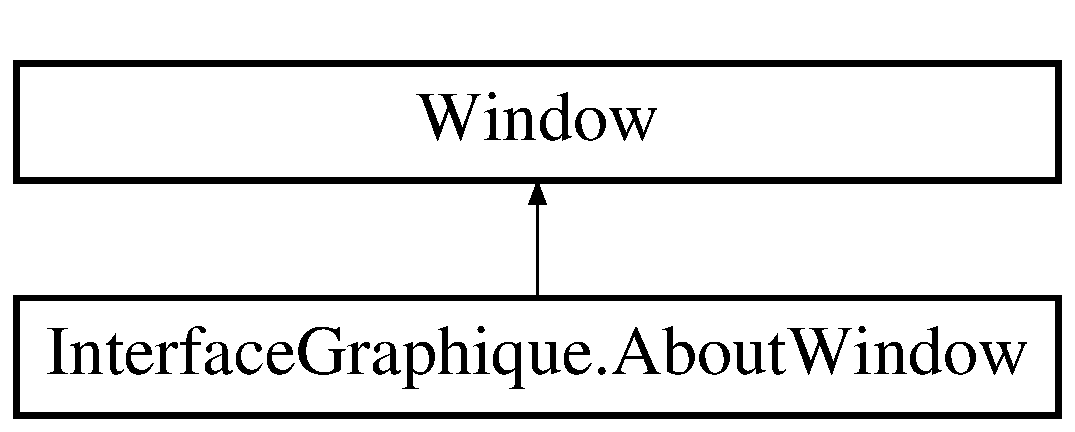
\includegraphics[height=2.000000cm]{class_interface_graphique_1_1_about_window}
\end{center}
\end{figure}


\subsection{Description détaillée}
Interaction logic for About\-Window.\-xaml 



La documentation de cette classe a été générée à partir du fichier suivant \-:\begin{DoxyCompactItemize}
\item 
C\-:/\-Users/saron/\-Documents/inf2990-\/01/\-Sources/\-Interface\-Graphique/About\-Window.\-xaml.\-cs\end{DoxyCompactItemize}

\hypertarget{classai_matrix4x4t}{\section{Référence du modèle de la classe ai\-Matrix4x4t$<$ T $>$}
\label{classai_matrix4x4t}\index{ai\-Matrix4x4t$<$ T $>$@{ai\-Matrix4x4t$<$ T $>$}}
}


La documentation de cette classe a été générée à partir du fichier suivant \-:\begin{DoxyCompactItemize}
\item 
C\-:/\-Users/saron/\-Documents/inf2990-\/01/\-Commun/\-Utilitaire/\hyperlink{_utilitaire_8h}{Utilitaire.\-h}\end{DoxyCompactItemize}

\hypertarget{class_angle_tool}{\section{Référence de la classe Angle\-Tool}
\label{class_angle_tool}\index{Angle\-Tool@{Angle\-Tool}}
}


Classe concrète héritant de \hyperlink{class_tool}{Tool}, qui effectue l'opération d'enregistrement de l'angle sur un noeud de l'arbre de rendu.  




{\ttfamily \#include $<$Angle\-Tool.\-h$>$}

Graphe d'héritage de Angle\-Tool\-:\begin{figure}[H]
\begin{center}
\leavevmode
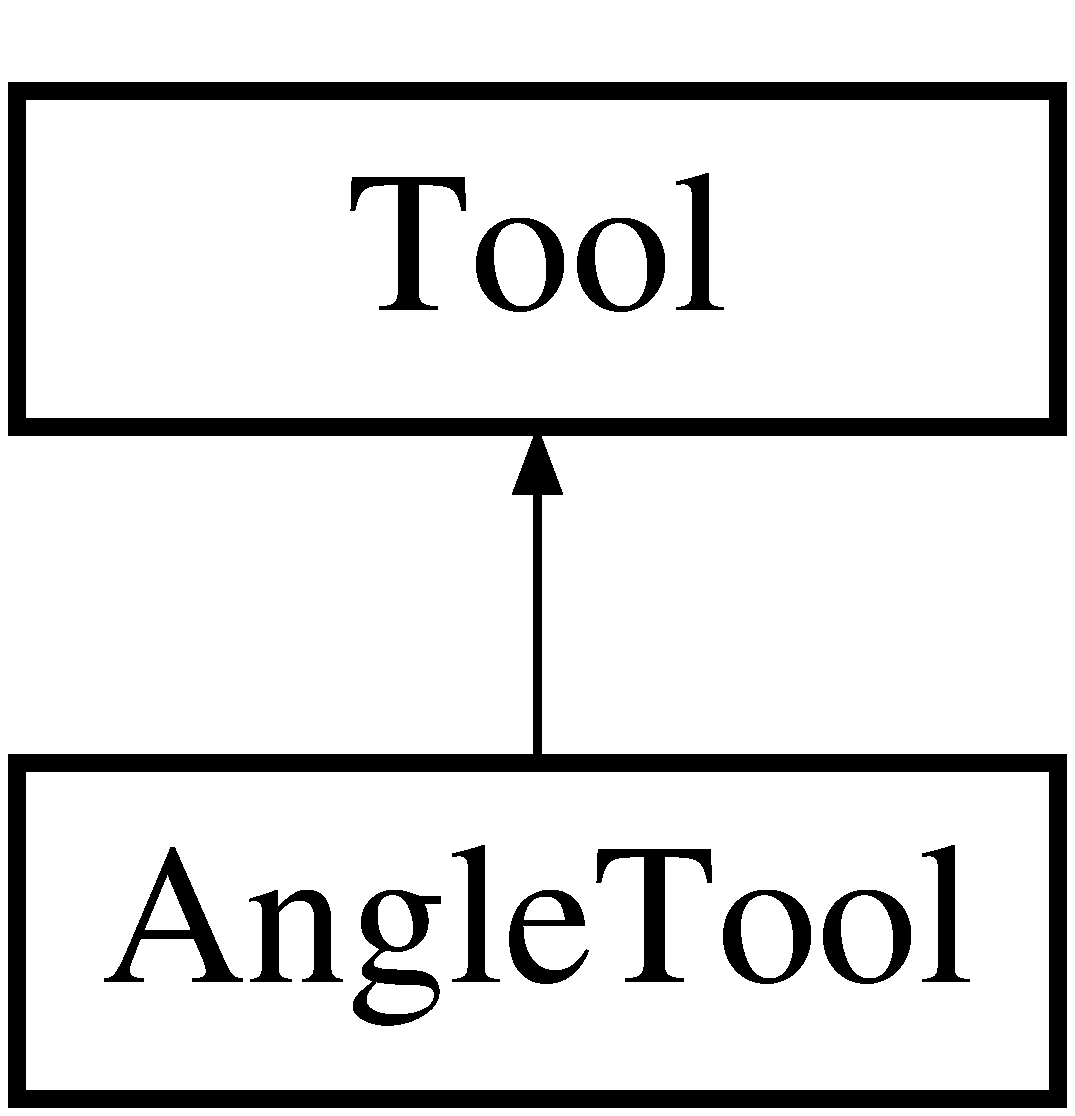
\includegraphics[height=2.000000cm]{class_angle_tool}
\end{center}
\end{figure}
\subsection*{Fonctions membres publiques}
\begin{DoxyCompactItemize}
\item 
void \hyperlink{group__inf2990_ga925fee2b000babaae1c7947a732a0bba}{visit} (\hyperlink{class_noeud_cylindre}{Noeud\-Cylindre} $\ast$node) override
\item 
void \hyperlink{group__inf2990_gaaa2fc24bde51948c2288c375f19d70ae}{visit} (\hyperlink{class_noeud_depart}{Noeud\-Depart} $\ast$node) override
\item 
void \hyperlink{group__inf2990_ga0209990747f5f623c71076c02a3ed018}{visit} (\hyperlink{class_noeud_segment_concret}{Noeud\-Segment\-Concret} $\ast$node) override
\item 
void \hyperlink{group__inf2990_ga5bf124eb8955a829e87743cc6a737b49}{visit} (\hyperlink{class_noeud_mur}{Noeud\-Mur} $\ast$node) override
\item 
void \hyperlink{group__inf2990_gac864ba35d8073ed9564a0a90d4df351d}{default\-Angle} (\hyperlink{class_noeud_abstrait}{Noeud\-Abstrait} $\ast$node)
\begin{DoxyCompactList}\small\item\em Algorithme par défaut. \end{DoxyCompactList}\end{DoxyCompactItemize}


\subsection{Description détaillée}
Classe concrète héritant de \hyperlink{class_tool}{Tool}, qui effectue l'opération d'enregistrement de l'angle sur un noeud de l'arbre de rendu. 

\begin{DoxyAuthor}{Auteur}
I\-N\-F2990-\/\-A15-\/01 
\end{DoxyAuthor}
\begin{DoxyDate}{Date}
2015-\/09-\/25 
\end{DoxyDate}


La documentation de cette classe a été générée à partir des fichiers suivants \-:\begin{DoxyCompactItemize}
\item 
C\-:/\-Users/saron/\-Documents/inf2990-\/01/\-Sources/\-D\-L\-L/\-Application/\-Visitor/\hyperlink{_angle_tool_8h}{Angle\-Tool.\-h}\item 
C\-:/\-Users/saron/\-Documents/inf2990-\/01/\-Sources/\-D\-L\-L/\-Application/\-Visitor/\hyperlink{_angle_tool_8cpp}{Angle\-Tool.\-cpp}\end{DoxyCompactItemize}

\hypertarget{class_arbre_rendu}{}\section{Arbre\+Rendu Class Reference}
\label{class_arbre_rendu}\index{Arbre\+Rendu@{Arbre\+Rendu}}


Classe d\textquotesingle{}arbre de rendu qui contient la racine de l\textquotesingle{}arbre de rendu avec les usines qui permettent d\textquotesingle{}ajouter des noeuds à cet arbre.  




{\ttfamily \#include $<$Arbre\+Rendu.\+h$>$}

Inheritance diagram for Arbre\+Rendu\+:\begin{figure}[H]
\begin{center}
\leavevmode
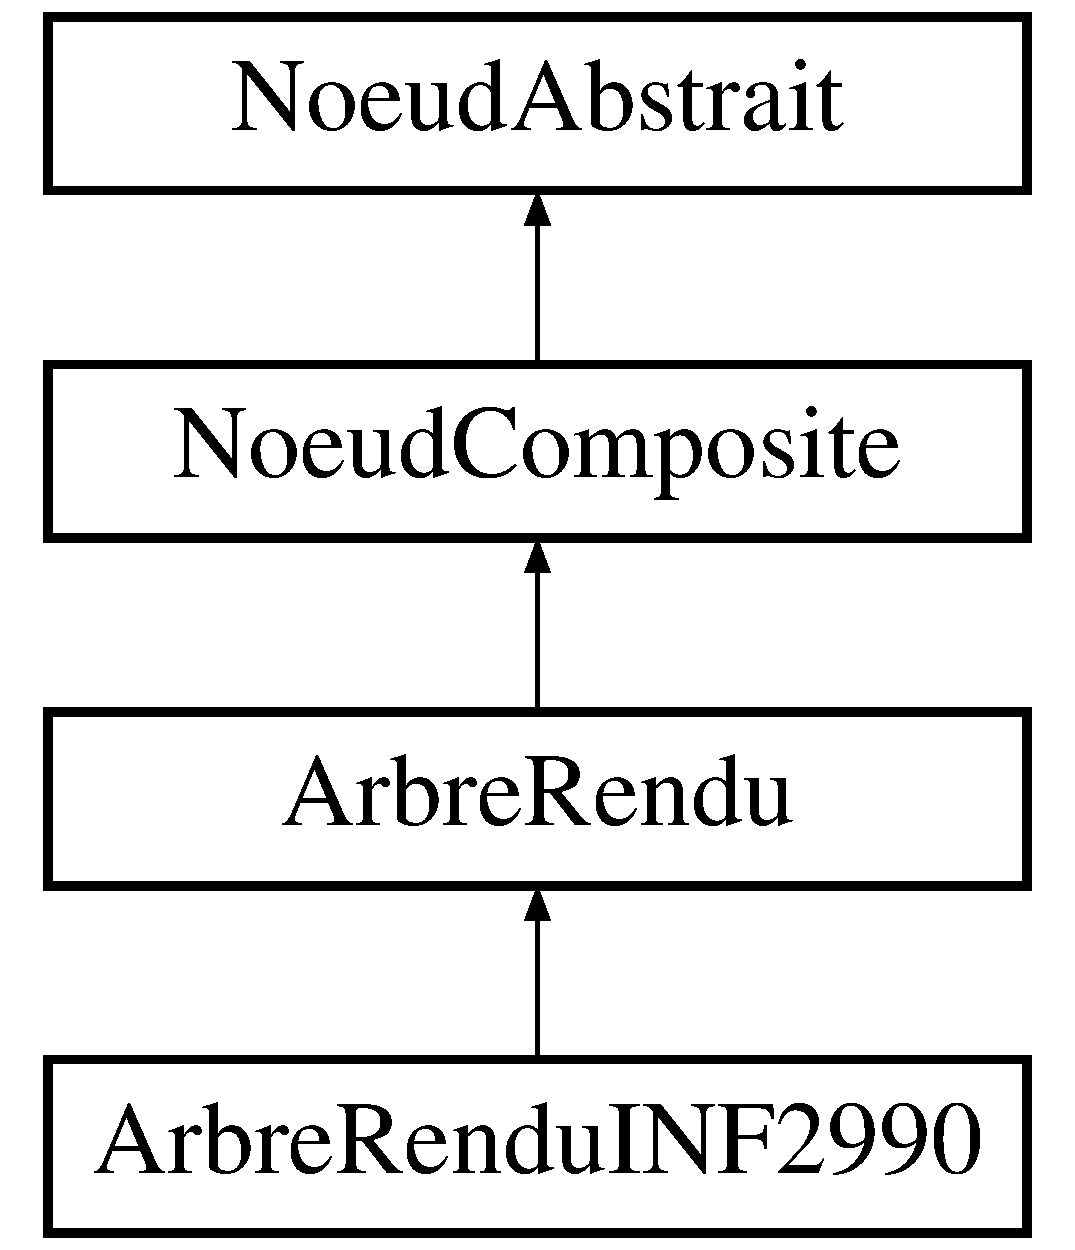
\includegraphics[height=4.000000cm]{class_arbre_rendu}
\end{center}
\end{figure}
\subsection*{Public Member Functions}
\begin{DoxyCompactItemize}
\item 
\hyperlink{group__inf2990_gaef1e98a66c4f1d3b468c786edee45ae6}{Arbre\+Rendu} ()
\begin{DoxyCompactList}\small\item\em Constructeur par défaut. \end{DoxyCompactList}\item 
virtual \hyperlink{group__inf2990_gadb462923759da0ff632dad097b7bfdab}{$\sim$\+Arbre\+Rendu} ()
\begin{DoxyCompactList}\small\item\em Destructeur. \end{DoxyCompactList}\item 
void \hyperlink{group__inf2990_ga296a744837fb7b779fadf2e8c62e6577}{ajouter\+Usine} (const std\+::string \&type, const \hyperlink{class_usine_abstraite}{Usine\+Abstraite} $\ast$usine)
\begin{DoxyCompactList}\small\item\em Ajoute une usine associée à un type de noeud. \end{DoxyCompactList}\item 
std\+::unique\+\_\+ptr$<$ \hyperlink{class_noeud_abstrait}{Noeud\+Abstrait} $>$ \hyperlink{group__inf2990_gaead1f3ae9de5de53e31ad9e886ba259c}{creer\+Noeud} (const std\+::string \&type\+Nouveau\+Noeud) const 
\begin{DoxyCompactList}\small\item\em Crée un nouveau noeud. \end{DoxyCompactList}\item 
\hyperlink{class_noeud_abstrait}{Noeud\+Abstrait} $\ast$ \hyperlink{group__inf2990_gac10e5f0623af502d67f72aef764206a3}{ajouter\+Nouveau\+Noeud} (const std\+::string \&nom\+Parent, const std\+::string \&type\+Nouveau\+Noeud)
\begin{DoxyCompactList}\small\item\em Crée et ajoute un nouveau noeud à l\textquotesingle{}arbre. \end{DoxyCompactList}\end{DoxyCompactItemize}
\subsection*{Static Public Member Functions}
\begin{DoxyCompactItemize}
\item 
static unsigned int \hyperlink{group__inf2990_gacf0e53d52040b07cd6550fda79867bd5}{calculer\+Profondeur\+Maximale} ()
\begin{DoxyCompactList}\small\item\em Calcule la profondeur maximale possible pour l\textquotesingle{}arbre de rendu. \end{DoxyCompactList}\end{DoxyCompactItemize}
\subsection*{Additional Inherited Members}


\subsection{Detailed Description}
Classe d\textquotesingle{}arbre de rendu qui contient la racine de l\textquotesingle{}arbre de rendu avec les usines qui permettent d\textquotesingle{}ajouter des noeuds à cet arbre. 

La profondeur de cet arbre est limitée par la taille de la pile des matrices et la taille de la pile des noms pour la sélection Open\+G\+L, étant donné que chaque niveau de l\textquotesingle{}arbre effectue un \char`\"{}push\char`\"{} sur chacune de ces piles lors du rendu. L\textquotesingle{}arbre ne vérifie pas que la profondeur reste sous la limite, mais il offre des fonctions permettant de le vérifier aisément.

\begin{DoxyAuthor}{Author}
Martin Bisson 
\end{DoxyAuthor}
\begin{DoxyDate}{Date}
2007-\/01-\/28 
\end{DoxyDate}


The documentation for this class was generated from the following files\+:\begin{DoxyCompactItemize}
\item 
C\+:/\+Users/\+Louis/workspace/inf2990-\/01/\+Sources/\+D\+L\+L/\+Arbre/\hyperlink{_arbre_rendu_8h}{Arbre\+Rendu.\+h}\item 
C\+:/\+Users/\+Louis/workspace/inf2990-\/01/\+Sources/\+D\+L\+L/\+Arbre/\hyperlink{_arbre_rendu_8cpp}{Arbre\+Rendu.\+cpp}\end{DoxyCompactItemize}

\hypertarget{class_arbre_rendu_i_n_f2990}{}\section{Arbre\+Rendu\+I\+N\+F2990 Class Reference}
\label{class_arbre_rendu_i_n_f2990}\index{Arbre\+Rendu\+I\+N\+F2990@{Arbre\+Rendu\+I\+N\+F2990}}


Classe qui représente l\textquotesingle{}arbre de rendu spécifique au projet de I\+N\+F2990.  




{\ttfamily \#include $<$Arbre\+Rendu\+I\+N\+F2990.\+h$>$}

Inheritance diagram for Arbre\+Rendu\+I\+N\+F2990\+:\begin{figure}[H]
\begin{center}
\leavevmode
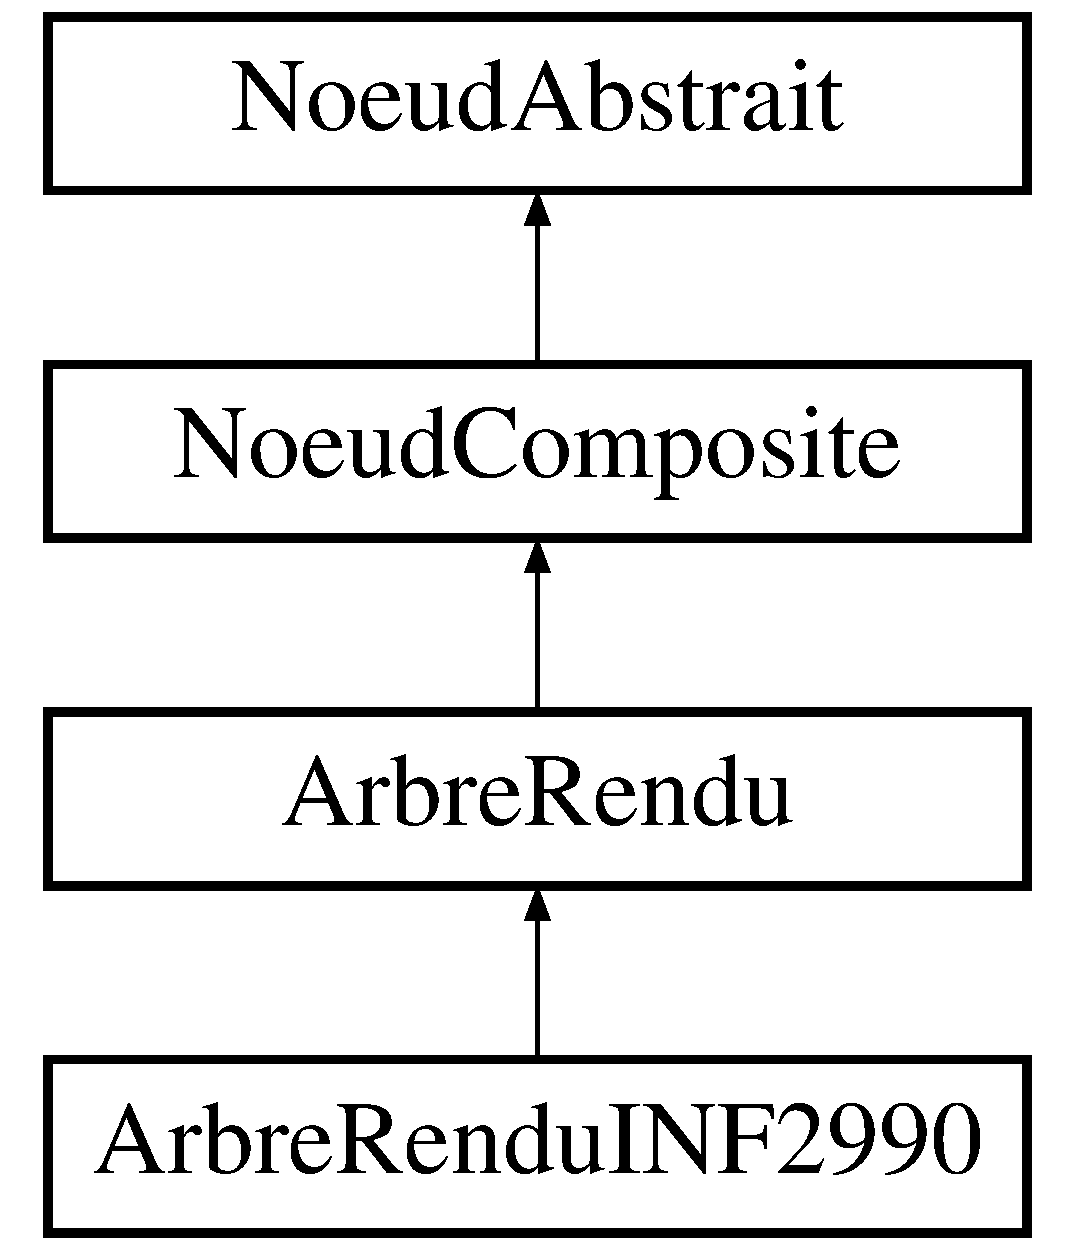
\includegraphics[height=4.000000cm]{class_arbre_rendu_i_n_f2990}
\end{center}
\end{figure}
\subsection*{Public Member Functions}
\begin{DoxyCompactItemize}
\item 
\hyperlink{group__inf2990_ga67528b7fa54e8ef8f96ef2e0bad06d2d}{Arbre\+Rendu\+I\+N\+F2990} ()
\begin{DoxyCompactList}\small\item\em Constructeur par défaut. \end{DoxyCompactList}\item 
virtual \hyperlink{group__inf2990_gaa67526b2fd719f6bcef7a4547bd25c7b}{$\sim$\+Arbre\+Rendu\+I\+N\+F2990} ()
\begin{DoxyCompactList}\small\item\em Destructeur. \end{DoxyCompactList}\item 
void \hyperlink{group__inf2990_ga678d89e1f12ae16ee7dcf6de3db637a3}{initialiser} ()
\begin{DoxyCompactList}\small\item\em Initialise l\textquotesingle{}arbre de rendu à son état initial. \end{DoxyCompactList}\end{DoxyCompactItemize}
\subsection*{Static Public Attributes}
\begin{DoxyCompactItemize}
\item 
\hypertarget{group__inf2990_ga1035430c1c08b95d17f891ae89b33b80}{}static const std\+::string \hyperlink{group__inf2990_ga1035430c1c08b95d17f891ae89b33b80}{N\+O\+M\+\_\+\+A\+R\+A\+I\+G\+N\+E\+E} \{ \char`\"{}araignee\char`\"{} \}\label{group__inf2990_ga1035430c1c08b95d17f891ae89b33b80}

\begin{DoxyCompactList}\small\item\em La chaîne représentant le type des araignées. \end{DoxyCompactList}\item 
\hypertarget{group__inf2990_gae849656178f4dad34106f525bf37341a}{}static const std\+::string \hyperlink{group__inf2990_gae849656178f4dad34106f525bf37341a}{N\+O\+M\+\_\+\+C\+O\+N\+E\+C\+U\+B\+E} \{ \char`\"{}conecube\char`\"{} \}\label{group__inf2990_gae849656178f4dad34106f525bf37341a}

\begin{DoxyCompactList}\small\item\em La chaîne représentant le type des cones-\/cubes. \end{DoxyCompactList}\item 
\hypertarget{group__inf2990_ga9a6799aa8903b858929bf675e4468aac}{}static const std\+::string \hyperlink{group__inf2990_ga9a6799aa8903b858929bf675e4468aac}{N\+O\+M\+\_\+\+R\+O\+B\+O\+T} \{ \char`\"{}robot\char`\"{} \}\label{group__inf2990_ga9a6799aa8903b858929bf675e4468aac}

\begin{DoxyCompactList}\small\item\em La chaîne représentant le type du robot. \end{DoxyCompactList}\item 
\hypertarget{group__inf2990_ga89e651c1a28481ce70f473bd15555114}{}static const std\+::string \hyperlink{group__inf2990_ga89e651c1a28481ce70f473bd15555114}{N\+O\+M\+\_\+\+T\+A\+B\+L\+E} \{ \char`\"{}table\char`\"{} \}\label{group__inf2990_ga89e651c1a28481ce70f473bd15555114}

\begin{DoxyCompactList}\small\item\em La chaîne représentant le type de la table. \end{DoxyCompactList}\item 
\hypertarget{group__inf2990_gae74e1de66e37dee6ef6cb6df82424c0d}{}static const std\+::string \hyperlink{group__inf2990_gae74e1de66e37dee6ef6cb6df82424c0d}{N\+O\+M\+\_\+\+C\+Y\+L\+I\+N\+D\+R\+E} \{ \char`\"{}cylindre\char`\"{} \}\label{group__inf2990_gae74e1de66e37dee6ef6cb6df82424c0d}

\begin{DoxyCompactList}\small\item\em La chaîne représentant le type du cylindre. \end{DoxyCompactList}\item 
\hypertarget{group__inf2990_ga4d9c8c9bfa165dde522834dec2882039}{}static const std\+::string \hyperlink{group__inf2990_ga4d9c8c9bfa165dde522834dec2882039}{N\+O\+M\+\_\+\+M\+U\+R} \{ \char`\"{}mur\char`\"{} \}\label{group__inf2990_ga4d9c8c9bfa165dde522834dec2882039}

\begin{DoxyCompactList}\small\item\em La chaîne représentant le type du mur. \end{DoxyCompactList}\item 
\hypertarget{group__inf2990_ga7f23ccbd07f9afea9685f108c4053834}{}static const std\+::string \hyperlink{group__inf2990_ga7f23ccbd07f9afea9685f108c4053834}{N\+O\+M\+\_\+\+D\+E\+P\+A\+R\+T} \{ \char`\"{}depart\char`\"{} \}\label{group__inf2990_ga7f23ccbd07f9afea9685f108c4053834}

\begin{DoxyCompactList}\small\item\em La chaîne représentant le spawn point. \end{DoxyCompactList}\end{DoxyCompactItemize}
\subsection*{Additional Inherited Members}


\subsection{Detailed Description}
Classe qui représente l\textquotesingle{}arbre de rendu spécifique au projet de I\+N\+F2990. 

Cette classe s\textquotesingle{}occupe de configurer les usines des noeuds qui seront utilisés par le projet.

\begin{DoxyAuthor}{Author}
Martin Bisson 
\end{DoxyAuthor}
\begin{DoxyDate}{Date}
2007-\/03-\/23 
\end{DoxyDate}


The documentation for this class was generated from the following files\+:\begin{DoxyCompactItemize}
\item 
Sources/\+D\+L\+L/\+Arbre/\hyperlink{_arbre_rendu_i_n_f2990_8h}{Arbre\+Rendu\+I\+N\+F2990.\+h}\item 
Sources/\+D\+L\+L/\+Arbre/\hyperlink{_arbre_rendu_i_n_f2990_8cpp}{Arbre\+Rendu\+I\+N\+F2990.\+cpp}\end{DoxyCompactItemize}

\hypertarget{class_avoid_left}{\section{Référence de la classe Avoid\-Left}
\label{class_avoid_left}\index{Avoid\-Left@{Avoid\-Left}}
}


Classe Etat du comportement \char`\"{}Évitement par la gauche\char`\"{}.  




{\ttfamily \#include $<$Avoid\-Left.\-h$>$}

Graphe d'héritage de Avoid\-Left\-:\begin{figure}[H]
\begin{center}
\leavevmode
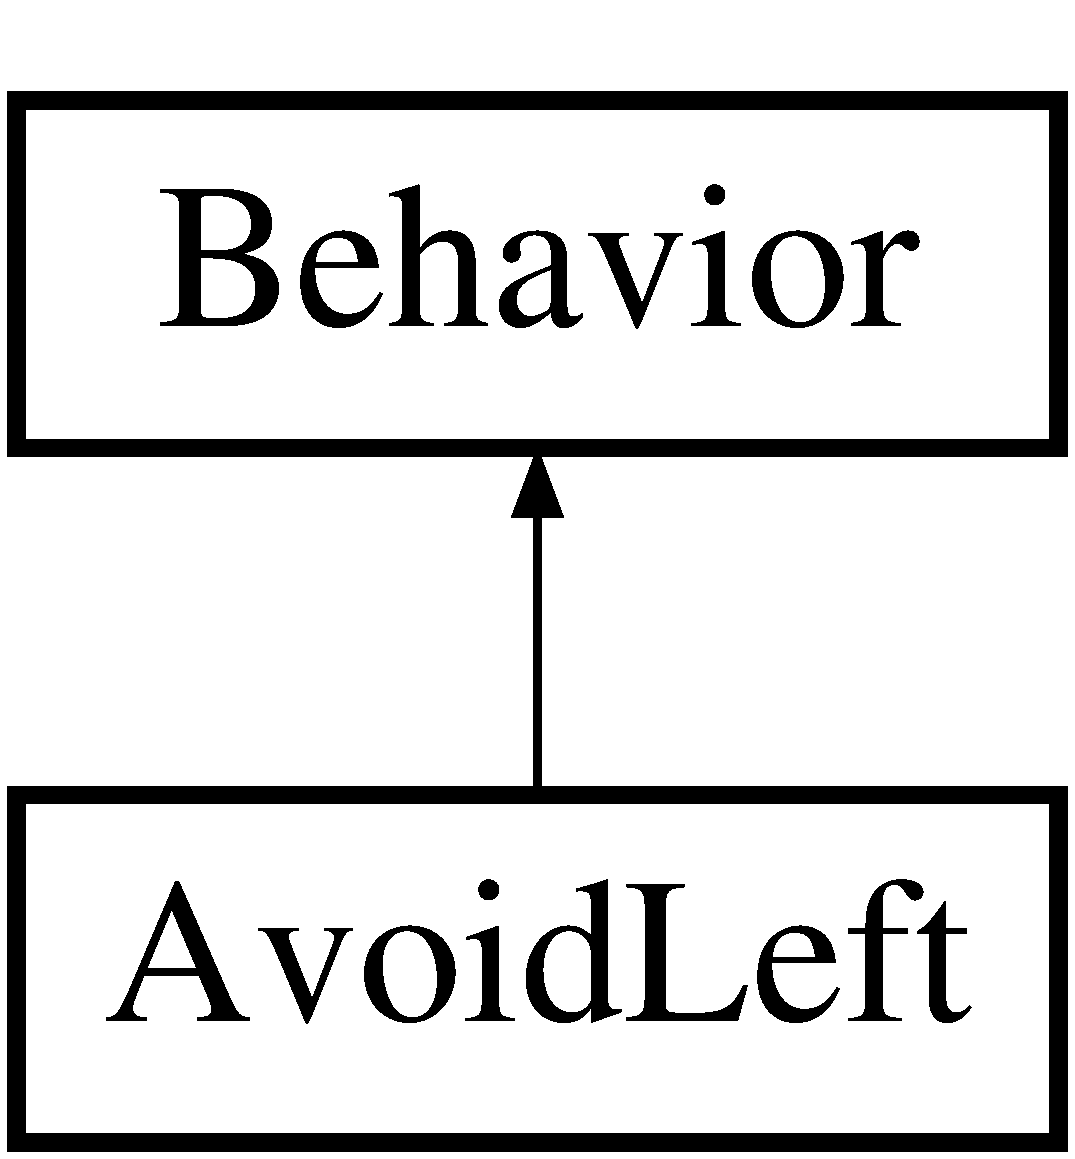
\includegraphics[height=2.000000cm]{class_avoid_left}
\end{center}
\end{figure}
\subsection*{Fonctions membres publiques}
{\bf }\par
\begin{DoxyCompactItemize}
\item 
\hyperlink{class_avoid_left_a0ef7b8c66b6fcfa50b3e80c817e59c18}{Avoid\-Left} (\hyperlink{class_behavior_context}{Behavior\-Context} $\ast$context)
\begin{DoxyCompactList}\small\item\em Constructeur. \end{DoxyCompactList}\item 
void \hyperlink{class_avoid_left_ab2c9b09f40a6e435a54e5c8ace316bfd}{do\-Action} () override
\begin{DoxyCompactList}\small\item\em Effectue une etape de son comportement. \end{DoxyCompactList}\end{DoxyCompactItemize}

\subsection*{Membres hérités additionnels}


\subsection{Description détaillée}
Classe Etat du comportement \char`\"{}Évitement par la gauche\char`\"{}. 

\subsection{Documentation des constructeurs et destructeur}
\hypertarget{class_avoid_left_a0ef7b8c66b6fcfa50b3e80c817e59c18}{\index{Avoid\-Left@{Avoid\-Left}!Avoid\-Left@{Avoid\-Left}}
\index{Avoid\-Left@{Avoid\-Left}!AvoidLeft@{Avoid\-Left}}
\subsubsection[{Avoid\-Left}]{\setlength{\rightskip}{0pt plus 5cm}Avoid\-Left\-::\-Avoid\-Left (
\begin{DoxyParamCaption}
\item[{{\bf Behavior\-Context} $\ast$}]{context}
\end{DoxyParamCaption}
)}}\label{class_avoid_left_a0ef7b8c66b6fcfa50b3e80c817e59c18}


Constructeur. 

Constructeur


\begin{DoxyParams}[1]{Paramètres}
\mbox{\tt in}  & {\em context} & \-: La classe pouvant accéder au robot.\\
\hline
\end{DoxyParams}
\begin{DoxyReturn}{Renvoie}
Aucune. 
\end{DoxyReturn}


\subsection{Documentation des fonctions membres}
\hypertarget{class_avoid_left_ab2c9b09f40a6e435a54e5c8ace316bfd}{\index{Avoid\-Left@{Avoid\-Left}!do\-Action@{do\-Action}}
\index{do\-Action@{do\-Action}!AvoidLeft@{Avoid\-Left}}
\subsubsection[{do\-Action}]{\setlength{\rightskip}{0pt plus 5cm}void Avoid\-Left\-::do\-Action (
\begin{DoxyParamCaption}
{}
\end{DoxyParamCaption}
)\hspace{0.3cm}{\ttfamily [override]}, {\ttfamily [virtual]}}}\label{class_avoid_left_ab2c9b09f40a6e435a54e5c8ace316bfd}


Effectue une etape de son comportement. 

Cette fonction effectue le comportement de l'état actuel.


\begin{DoxyParams}[1]{Paramètres}
\mbox{\tt in}  & {\em Aucun.} & \\
\hline
\end{DoxyParams}
\begin{DoxyReturn}{Renvoie}
Aucune. 
\end{DoxyReturn}


Réimplémentée à partir de \hyperlink{group__inf2990_gac22f205bc85075ff707ad1f695c18439}{Behavior}.



La documentation de cette classe a été générée à partir des fichiers suivants \-:\begin{DoxyCompactItemize}
\item 
C\-:/\-Users/saron/\-Documents/inf2990-\/01/\-Sources/\-D\-L\-L/\-Behavior/\hyperlink{_avoid_left_8h}{Avoid\-Left.\-h}\item 
C\-:/\-Users/saron/\-Documents/inf2990-\/01/\-Sources/\-D\-L\-L/\-Behavior/\hyperlink{_avoid_left_8cpp}{Avoid\-Left.\-cpp}\item 
C\-:/\-Users/saron/\-Documents/inf2990-\/01/\-Sources/\-D\-L\-L/\-Behavior/\hyperlink{_avoid_right_8cpp}{Avoid\-Right.\-cpp}\end{DoxyCompactItemize}

\hypertarget{class_avoid_right}{\section{Référence de la classe Avoid\-Right}
\label{class_avoid_right}\index{Avoid\-Right@{Avoid\-Right}}
}


Classe Etat du comportement \char`\"{}Évitement par la droite\char`\"{}.  




{\ttfamily \#include $<$Avoid\-Right.\-h$>$}

Graphe d'héritage de Avoid\-Right\-:\begin{figure}[H]
\begin{center}
\leavevmode
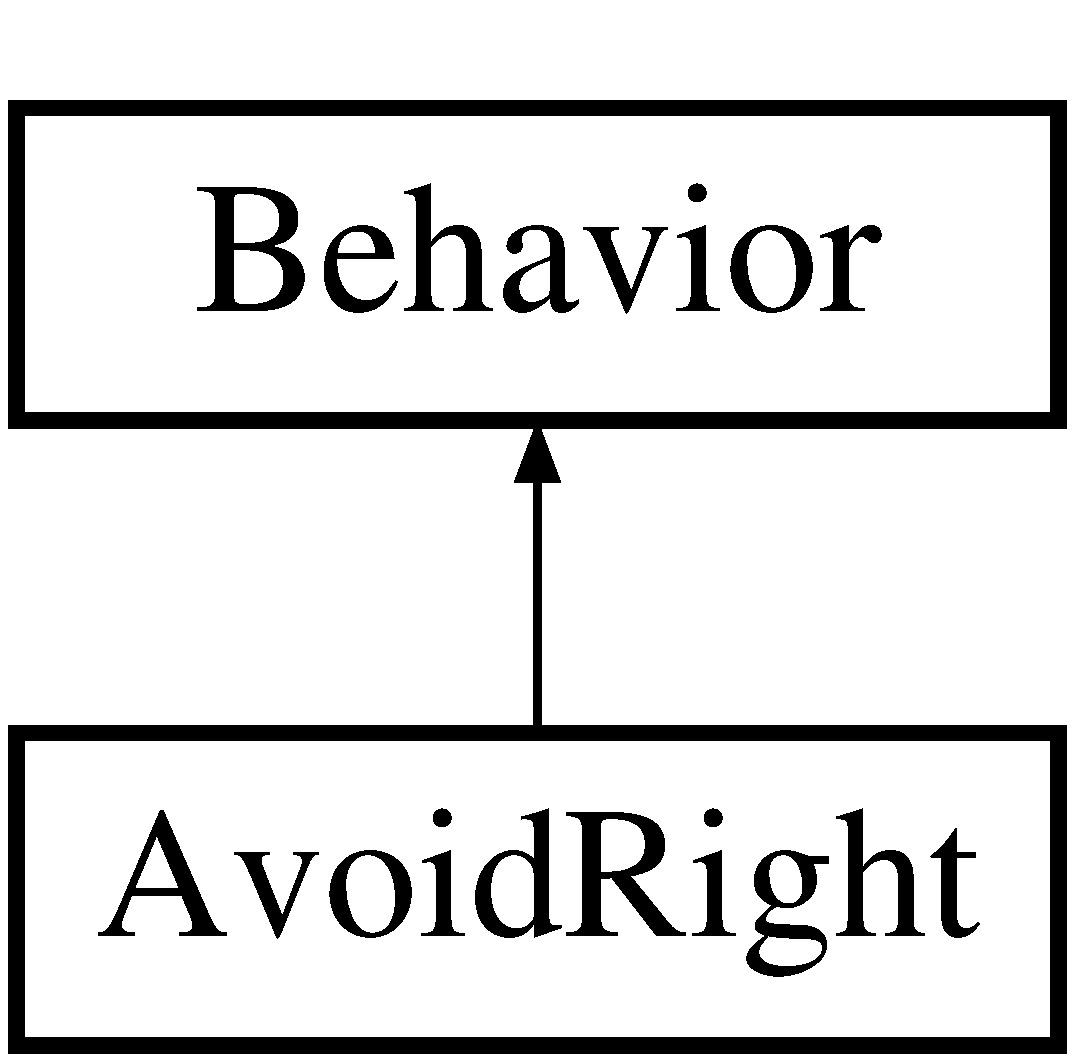
\includegraphics[height=2.000000cm]{class_avoid_right}
\end{center}
\end{figure}
\subsection*{Fonctions membres publiques}
{\bf }\par
\begin{DoxyCompactItemize}
\item 
\hyperlink{class_avoid_right_a0ab41a5c688b5cc3f66bc107feb03014}{Avoid\-Right} (\hyperlink{class_behavior_context}{Behavior\-Context} $\ast$context)
\begin{DoxyCompactList}\small\item\em Constructeur. \end{DoxyCompactList}\item 
\hypertarget{class_avoid_right_a58ad8275468349660d17d26867e33225}{void \hyperlink{class_avoid_right_a58ad8275468349660d17d26867e33225}{do\-Action} () override}\label{class_avoid_right_a58ad8275468349660d17d26867e33225}

\begin{DoxyCompactList}\small\item\em Effectue une etape de son comportement. \end{DoxyCompactList}\end{DoxyCompactItemize}

\subsection*{Membres hérités additionnels}


\subsection{Description détaillée}
Classe Etat du comportement \char`\"{}Évitement par la droite\char`\"{}. 

\subsection{Documentation des constructeurs et destructeur}
\hypertarget{class_avoid_right_a0ab41a5c688b5cc3f66bc107feb03014}{\index{Avoid\-Right@{Avoid\-Right}!Avoid\-Right@{Avoid\-Right}}
\index{Avoid\-Right@{Avoid\-Right}!AvoidRight@{Avoid\-Right}}
\subsubsection[{Avoid\-Right}]{\setlength{\rightskip}{0pt plus 5cm}Avoid\-Right\-::\-Avoid\-Right (
\begin{DoxyParamCaption}
\item[{{\bf Behavior\-Context} $\ast$}]{context}
\end{DoxyParamCaption}
)}}\label{class_avoid_right_a0ab41a5c688b5cc3f66bc107feb03014}


Constructeur. 

Constructeur


\begin{DoxyParams}[1]{Paramètres}
\mbox{\tt in}  & {\em context} & \-: La classe pouvant accéder au robot.\\
\hline
\end{DoxyParams}
\begin{DoxyReturn}{Renvoie}
Aucune. 
\end{DoxyReturn}


La documentation de cette classe a été générée à partir des fichiers suivants \-:\begin{DoxyCompactItemize}
\item 
C\-:/\-Users/saron/\-Documents/inf2990-\/01/\-Sources/\-D\-L\-L/\-Behavior/\hyperlink{_avoid_right_8h}{Avoid\-Right.\-h}\item 
C\-:/\-Users/saron/\-Documents/inf2990-\/01/\-Sources/\-D\-L\-L/\-Behavior/\hyperlink{_avoid_right_8cpp}{Avoid\-Right.\-cpp}\end{DoxyCompactItemize}

\hypertarget{class_banc_tests}{\section{Référence de la classe Banc\-Tests}
\label{class_banc_tests}\index{Banc\-Tests@{Banc\-Tests}}
}


Banc de tests qui permet d'exécuter tous les tests unitaires. C'est une classe singleton.  




{\ttfamily \#include $<$Banc\-Tests.\-h$>$}

Graphe d'héritage de Banc\-Tests\-:\begin{figure}[H]
\begin{center}
\leavevmode
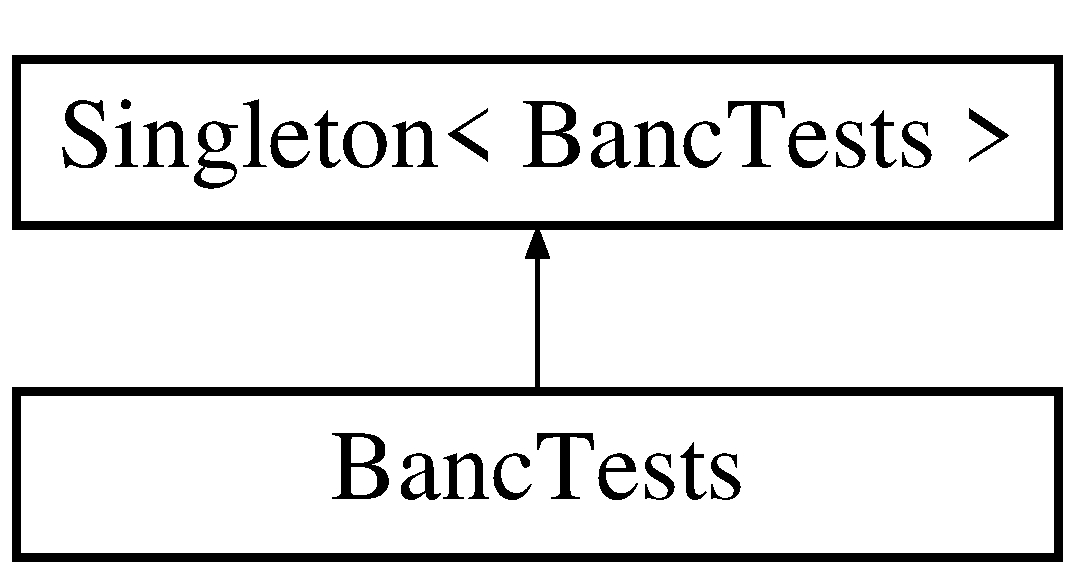
\includegraphics[height=2.000000cm]{class_banc_tests}
\end{center}
\end{figure}
\subsection*{Fonctions membres publiques}
\begin{DoxyCompactItemize}
\item 
bool \hyperlink{group__inf2990_gab5d7fbfe7e3fbe00aa187caa10b1c506}{executer} ()
\begin{DoxyCompactList}\small\item\em Exécuter tous les tests unitaires. \end{DoxyCompactList}\end{DoxyCompactItemize}
\subsection*{Membres hérités additionnels}


\subsection{Description détaillée}
Banc de tests qui permet d'exécuter tous les tests unitaires. C'est une classe singleton. 

\begin{DoxyAuthor}{Auteur}
Julien Gascon-\/\-Samson 
\end{DoxyAuthor}
\begin{DoxyDate}{Date}
2011-\/07-\/16 
\end{DoxyDate}


La documentation de cette classe a été générée à partir des fichiers suivants \-:\begin{DoxyCompactItemize}
\item 
C\-:/\-Users/saron/\-Documents/inf2990-\/01/\-Sources/\-D\-L\-L/\-Tests/\hyperlink{_banc_tests_8h}{Banc\-Tests.\-h}\item 
C\-:/\-Users/saron/\-Documents/inf2990-\/01/\-Sources/\-D\-L\-L/\-Tests/\hyperlink{_banc_tests_8cpp}{Banc\-Tests.\-cpp}\end{DoxyCompactItemize}

\hypertarget{class_behavior}{\section{Référence de la classe Behavior}
\label{class_behavior}\index{Behavior@{Behavior}}
}


Classe Etat du comportement par defaut.  


Graphe d'héritage de Behavior\-:\begin{figure}[H]
\begin{center}
\leavevmode
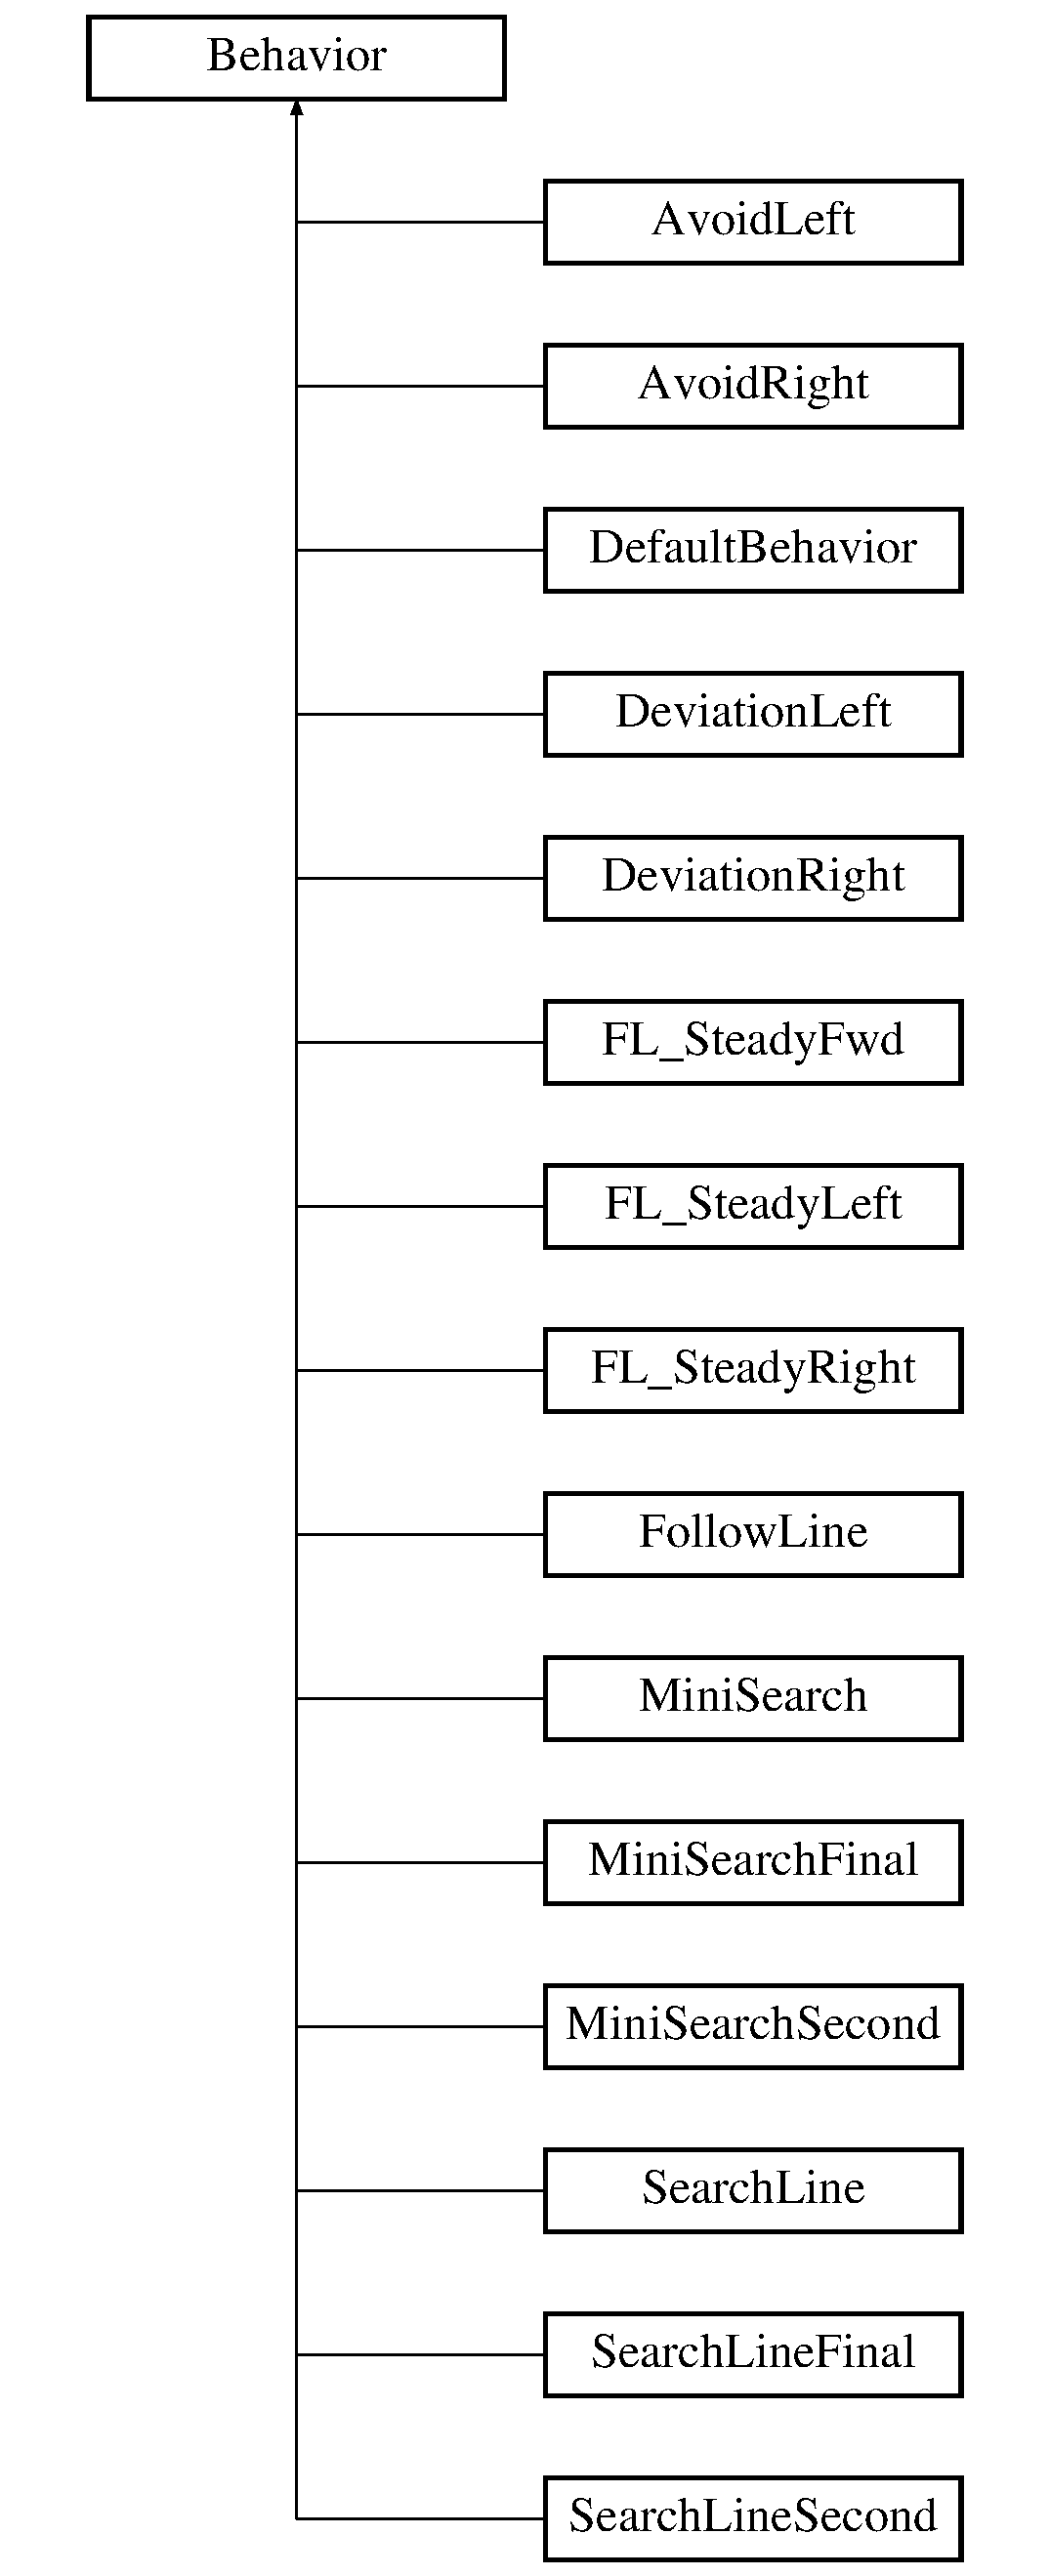
\includegraphics[height=12.000000cm]{class_behavior}
\end{center}
\end{figure}
\subsection*{Fonctions membres publiques}
\begin{DoxyCompactItemize}
\item 
\hypertarget{class_behavior_a335dc833288c48573797fa8eff3d04d5}{\hyperlink{class_behavior_a335dc833288c48573797fa8eff3d04d5}{Behavior} (\hyperlink{class_behavior_context}{Behavior\-Context} $\ast$context)}\label{class_behavior_a335dc833288c48573797fa8eff3d04d5}

\begin{DoxyCompactList}\small\item\em Constructeur. \end{DoxyCompactList}\end{DoxyCompactItemize}
{\bf }\par
\begin{DoxyCompactItemize}
\item 
virtual void \hyperlink{group__inf2990_gac22f205bc85075ff707ad1f695c18439}{do\-Action} ()
\begin{DoxyCompactList}\small\item\em Effectue une etape de son comportement. \end{DoxyCompactList}\end{DoxyCompactItemize}

\subsection*{Attributs protégés}
\begin{DoxyCompactItemize}
\item 
\hypertarget{class_behavior_ae794fb00dfe48b0eda2c564a9db92859}{\hyperlink{class_behavior_context}{Behavior\-Context} $\ast$ {\bfseries context\-\_\-}}\label{class_behavior_ae794fb00dfe48b0eda2c564a9db92859}

\end{DoxyCompactItemize}


\subsection{Description détaillée}
Classe Etat du comportement par defaut. 

La documentation de cette classe a été générée à partir des fichiers suivants \-:\begin{DoxyCompactItemize}
\item 
C\-:/\-Users/saron/\-Documents/inf2990-\/01/\-Sources/\-D\-L\-L/\-Behavior/\hyperlink{_behavior_8h}{Behavior.\-h}\item 
C\-:/\-Users/saron/\-Documents/inf2990-\/01/\-Sources/\-D\-L\-L/\-Behavior/\hyperlink{_behavior_8cpp}{Behavior.\-cpp}\item 
C\-:/\-Users/saron/\-Documents/inf2990-\/01/\-Sources/\-D\-L\-L/\-Behavior/\hyperlink{_behavior_context_8cpp}{Behavior\-Context.\-cpp}\end{DoxyCompactItemize}

\hypertarget{classbehavior}{\section{Référence de la classe behavior}
\label{classbehavior}\index{behavior@{behavior}}
}


Classe Etats contenant les comportements du robot.  




{\ttfamily \#include $<$Behavior.\-h$>$}



\subsection{Description détaillée}
Classe Etats contenant les comportements du robot. 

La documentation de cette classe a été générée à partir du fichier suivant \-:\begin{DoxyCompactItemize}
\item 
C\-:/\-Users/saron/\-Documents/inf2990-\/01/\-Sources/\-D\-L\-L/\-Behavior/\hyperlink{_behavior_8h}{Behavior.\-h}\end{DoxyCompactItemize}

\hypertarget{class_behavior_context}{\section{Référence de la classe Behavior\-Context}
\label{class_behavior_context}\index{Behavior\-Context@{Behavior\-Context}}
}


Classe Etats contenant les comportements du robot.  




{\ttfamily \#include $<$Behavior\-Context.\-h$>$}

\subsection*{Fonctions membres publiques}
\begin{DoxyCompactItemize}
\item 
\hypertarget{class_behavior_context_a0fdf61f6304296d6d0b868bc397e0b7b}{\hyperlink{class_behavior_context_a0fdf61f6304296d6d0b868bc397e0b7b}{Behavior\-Context} (\hyperlink{class_noeud_robot}{Noeud\-Robot} $\ast$robot)}\label{class_behavior_context_a0fdf61f6304296d6d0b868bc397e0b7b}

\begin{DoxyCompactList}\small\item\em Constructeur. \end{DoxyCompactList}\item 
\hypertarget{group__inf2990_ga2d15f4d9b398d9b3cb79f790dcf0187f}{void \hyperlink{group__inf2990_ga2d15f4d9b398d9b3cb79f790dcf0187f}{do\-Action} ()}\label{group__inf2990_ga2d15f4d9b398d9b3cb79f790dcf0187f}

\begin{DoxyCompactList}\small\item\em Effectue une etape de son comportement. \end{DoxyCompactList}\item 
\hypertarget{group__inf2990_gab48b5ca95ff1064b51a159e41e68fbaf}{void \hyperlink{group__inf2990_gab48b5ca95ff1064b51a159e41e68fbaf}{change\-Behavior} (std\-::unique\-\_\-ptr$<$ \hyperlink{class_behavior}{Behavior} $>$ state)}\label{group__inf2990_gab48b5ca95ff1064b51a159e41e68fbaf}

\begin{DoxyCompactList}\small\item\em Change l'etat actuel du robot. \end{DoxyCompactList}\item 
\hypertarget{group__inf2990_gab248d4182058e0746819e567d9fecbfb}{\hyperlink{class_noeud_robot}{Noeud\-Robot} $\ast$ \hyperlink{group__inf2990_gab248d4182058e0746819e567d9fecbfb}{get\-Robot} () const }\label{group__inf2990_gab248d4182058e0746819e567d9fecbfb}

\begin{DoxyCompactList}\small\item\em Envoi une reference observatrice vers le robot. \end{DoxyCompactList}\end{DoxyCompactItemize}


\subsection{Description détaillée}
Classe Etats contenant les comportements du robot. 

La documentation de cette classe a été générée à partir des fichiers suivants \-:\begin{DoxyCompactItemize}
\item 
C\-:/\-Users/saron/\-Documents/inf2990-\/01/\-Sources/\-D\-L\-L/\-Behavior/\hyperlink{_behavior_context_8h}{Behavior\-Context.\-h}\item 
C\-:/\-Users/saron/\-Documents/inf2990-\/01/\-Sources/\-D\-L\-L/\-Behavior/\hyperlink{_behavior_context_8cpp}{Behavior\-Context.\-cpp}\end{DoxyCompactItemize}

\hypertarget{structutilitaire_1_1_boite_englobante}{}\section{utilitaire\+:\+:Boite\+Englobante Struct Reference}
\label{structutilitaire_1_1_boite_englobante}\index{utilitaire\+::\+Boite\+Englobante@{utilitaire\+::\+Boite\+Englobante}}


Structure contenant les données pour une boite englobante.  




{\ttfamily \#include $<$Utilitaire.\+h$>$}

\subsection*{Public Attributes}
\begin{DoxyCompactItemize}
\item 
\hypertarget{structutilitaire_1_1_boite_englobante_a083f953a1ac5a830f70a2173a092e90a}{}glm\+::dvec3 {\bfseries coin\+Min}\label{structutilitaire_1_1_boite_englobante_a083f953a1ac5a830f70a2173a092e90a}

\item 
\hypertarget{structutilitaire_1_1_boite_englobante_af6f6d9ef23f6e5eb9f2f1ed6dd4d3e0e}{}glm\+::dvec3 {\bfseries coin\+Max}\label{structutilitaire_1_1_boite_englobante_af6f6d9ef23f6e5eb9f2f1ed6dd4d3e0e}

\end{DoxyCompactItemize}


\subsection{Detailed Description}
Structure contenant les données pour une boite englobante. 

The documentation for this struct was generated from the following file\+:\begin{DoxyCompactItemize}
\item 
Commun/\+Utilitaire/\hyperlink{_utilitaire_8h}{Utilitaire.\+h}\end{DoxyCompactItemize}

\hypertarget{classutilitaire_1_1_boite_environnement}{\section{Référence de la classe utilitaire\-:\-:Boite\-Environnement}
\label{classutilitaire_1_1_boite_environnement}\index{utilitaire\-::\-Boite\-Environnement@{utilitaire\-::\-Boite\-Environnement}}
}


Classe représentant une boîte d'environnement (\char`\"{}skybox\char`\"{}).  




{\ttfamily \#include $<$Boite\-Environnement.\-h$>$}

\subsection*{Fonctions membres publiques}
\begin{DoxyCompactItemize}
\item 
\hyperlink{classutilitaire_1_1_boite_environnement_afa2e429fd77f584d9b07e1577b907f7b}{Boite\-Environnement} (const std\-::string \&fichier\-Xpos, const std\-::string \&fichier\-Xneg, const std\-::string \&fichier\-Ypos, const std\-::string \&fichier\-Yneg, const std\-::string \&fichier\-Zpos, const std\-::string \&fichier\-Zneg)
\begin{DoxyCompactList}\small\item\em Constructeur à partir des noms des fichiers d'images de la boîte. \end{DoxyCompactList}\item 
\hyperlink{classutilitaire_1_1_boite_environnement_accfe35d5a88904e5001653142b985a27}{$\sim$\-Boite\-Environnement} ()
\begin{DoxyCompactList}\small\item\em Destructeur. \end{DoxyCompactList}\item 
void \hyperlink{classutilitaire_1_1_boite_environnement_a41246ea752945870645cfbd5aec673e9}{afficher} (const glm\-::dvec3 \&centre, double demi\-Largeur) const 
\begin{DoxyCompactList}\small\item\em Affiche la boîte d'environnement. \end{DoxyCompactList}\end{DoxyCompactItemize}


\subsection{Description détaillée}
Classe représentant une boîte d'environnement (\char`\"{}skybox\char`\"{}). 

Elle s'occupe de charger 6 images du cube formant la boîte. Elle utilise la convention de sens de Cube\-Map\-Gen (de A\-T\-I), lorsque les images sont exportées avec le mapping Open\-G\-L (plutôt que Direct\-X).

\begin{DoxyAuthor}{Auteur}
Martin Bisson 
\end{DoxyAuthor}
\begin{DoxyDate}{Date}
2007-\/05-\/28 
\end{DoxyDate}


\subsection{Documentation des constructeurs et destructeur}
\hypertarget{classutilitaire_1_1_boite_environnement_afa2e429fd77f584d9b07e1577b907f7b}{\index{utilitaire\-::\-Boite\-Environnement@{utilitaire\-::\-Boite\-Environnement}!Boite\-Environnement@{Boite\-Environnement}}
\index{Boite\-Environnement@{Boite\-Environnement}!utilitaire::BoiteEnvironnement@{utilitaire\-::\-Boite\-Environnement}}
\subsubsection[{Boite\-Environnement}]{\setlength{\rightskip}{0pt plus 5cm}utilitaire\-::\-Boite\-Environnement\-::\-Boite\-Environnement (
\begin{DoxyParamCaption}
\item[{const std\-::string \&}]{fichier\-Xpos, }
\item[{const std\-::string \&}]{fichier\-Xneg, }
\item[{const std\-::string \&}]{fichier\-Ypos, }
\item[{const std\-::string \&}]{fichier\-Yneg, }
\item[{const std\-::string \&}]{fichier\-Zpos, }
\item[{const std\-::string \&}]{fichier\-Zneg}
\end{DoxyParamCaption}
)}}\label{classutilitaire_1_1_boite_environnement_afa2e429fd77f584d9b07e1577b907f7b}


Constructeur à partir des noms des fichiers d'images de la boîte. 

Ce constructeur charge les 6 textures correspondant à chacune des faces de la boîte d'environnement.


\begin{DoxyParams}[1]{Paramètres}
\mbox{\tt in}  & {\em fichier\-Xpos} & \-: Le nom du fichier contenant l'image correspondant à l'axe des X positifs. \\
\hline
\mbox{\tt in}  & {\em fichier\-Xneg} & \-: Le nom du fichier contenant l'image correspondant à l'axe des X négatifs. \\
\hline
\mbox{\tt in}  & {\em fichier\-Ypos} & \-: Le nom du fichier contenant l'image correspondant à l'axe des X positifs. \\
\hline
\mbox{\tt in}  & {\em fichier\-Yneg} & \-: Le nom du fichier contenant l'image correspondant à l'axe des Y négatifs. \\
\hline
\mbox{\tt in}  & {\em fichier\-Zpos} & \-: Le nom du fichier contenant l'image correspondant à l'axe des Z positifs. \\
\hline
\mbox{\tt in}  & {\em fichier\-Zneg} & \-: Le nom du fichier contenant l'image correspondant à l'axe des Z négatifs.\\
\hline
\end{DoxyParams}
\begin{DoxyReturn}{Renvoie}
Aucune (constructeur). 
\end{DoxyReturn}
\hypertarget{classutilitaire_1_1_boite_environnement_accfe35d5a88904e5001653142b985a27}{\index{utilitaire\-::\-Boite\-Environnement@{utilitaire\-::\-Boite\-Environnement}!$\sim$\-Boite\-Environnement@{$\sim$\-Boite\-Environnement}}
\index{$\sim$\-Boite\-Environnement@{$\sim$\-Boite\-Environnement}!utilitaire::BoiteEnvironnement@{utilitaire\-::\-Boite\-Environnement}}
\subsubsection[{$\sim$\-Boite\-Environnement}]{\setlength{\rightskip}{0pt plus 5cm}utilitaire\-::\-Boite\-Environnement\-::$\sim$\-Boite\-Environnement (
\begin{DoxyParamCaption}
{}
\end{DoxyParamCaption}
)}}\label{classutilitaire_1_1_boite_environnement_accfe35d5a88904e5001653142b985a27}


Destructeur. 

Ce destructeur libère l'espace allouée à chacune des textures des faces de la boîte d'environnement.

\begin{DoxyReturn}{Renvoie}
Aucune (destructeur). 
\end{DoxyReturn}


\subsection{Documentation des fonctions membres}
\hypertarget{classutilitaire_1_1_boite_environnement_a41246ea752945870645cfbd5aec673e9}{\index{utilitaire\-::\-Boite\-Environnement@{utilitaire\-::\-Boite\-Environnement}!afficher@{afficher}}
\index{afficher@{afficher}!utilitaire::BoiteEnvironnement@{utilitaire\-::\-Boite\-Environnement}}
\subsubsection[{afficher}]{\setlength{\rightskip}{0pt plus 5cm}void utilitaire\-::\-Boite\-Environnement\-::afficher (
\begin{DoxyParamCaption}
\item[{const glm\-::dvec3 \&}]{centre, }
\item[{double}]{demi\-Largeur}
\end{DoxyParamCaption}
) const}}\label{classutilitaire_1_1_boite_environnement_a41246ea752945870645cfbd5aec673e9}


Affiche la boîte d'environnement. 

Cette fonction affiche tout simplement la boîte d'environnement.


\begin{DoxyParams}[1]{Paramètres}
\mbox{\tt in}  & {\em centre} & \-: La position du centre de la boîte pour l'affichage. \\
\hline
\mbox{\tt in}  & {\em demi\-Largeur} & \-: La largeur de la moitié de la boîte pour l'affichage.\\
\hline
\end{DoxyParams}
\begin{DoxyReturn}{Renvoie}
Aucune. 
\end{DoxyReturn}


La documentation de cette classe a été générée à partir des fichiers suivants \-:\begin{DoxyCompactItemize}
\item 
C\-:/\-Users/saron/\-Documents/inf2990-\/01/\-Commun/\-Utilitaire/\-Open\-G\-L/\hyperlink{_boite_environnement_8h}{Boite\-Environnement.\-h}\item 
C\-:/\-Users/saron/\-Documents/inf2990-\/01/\-Commun/\-Utilitaire/\-Open\-G\-L/\hyperlink{_boite_environnement_8cpp}{Boite\-Environnement.\-cpp}\end{DoxyCompactItemize}

\hypertarget{classvue_1_1_camera}{\section{Référence de la classe vue\-:\-:Camera}
\label{classvue_1_1_camera}\index{vue\-::\-Camera@{vue\-::\-Camera}}
}


Classe représentant une caméra dans le monde en 3\-D.  




{\ttfamily \#include $<$Camera.\-h$>$}

\subsection*{Fonctions membres publiques}
\begin{DoxyCompactItemize}
\item 
\hyperlink{classvue_1_1_camera_a0c7869e1153f216e88fc15eb5ac37ce4}{Camera} (const glm\-::dvec3 \&position, const glm\-::dvec3 \&point\-Vise, const glm\-::dvec3 \&direction\-Haut\-Camera, const glm\-::dvec3 \&direction\-Haut\-Monde)
\begin{DoxyCompactList}\small\item\em Constructeur à partir des coordonnées cartésiennes. \end{DoxyCompactList}\item 
\hypertarget{classvue_1_1_camera_a173cf3a9d91b30cadd21d72149df4504}{virtual \hyperlink{classvue_1_1_camera_a173cf3a9d91b30cadd21d72149df4504}{$\sim$\-Camera} ()}\label{classvue_1_1_camera_a173cf3a9d91b30cadd21d72149df4504}

\begin{DoxyCompactList}\small\item\em Destructeur virtuel vide. \end{DoxyCompactList}\item 
void \hyperlink{classvue_1_1_camera_a452efa2c96225b1207cc9ac74be0bda5}{assigner\-Position} (const glm\-::dvec3 \&position)
\begin{DoxyCompactList}\small\item\em Assigner la position de la caméra. \end{DoxyCompactList}\item 
void \hyperlink{classvue_1_1_camera_a73e6c0d4915b3ee6f007e0630fb7dcc0}{assigner\-Position\-Initiale} (const glm\-::dvec3 \&position)
\item 
void \hyperlink{classvue_1_1_camera_a0b9982453adc3afc38f9198ab8b1dd2a}{assigner\-Point\-Vise} (const glm\-::dvec3 \&point\-Vise)
\begin{DoxyCompactList}\small\item\em Assigner le point visé de la caméra. \end{DoxyCompactList}\item 
void \hyperlink{classvue_1_1_camera_a38a36bcc9a9039f20c1f00ea6266bffb}{assigner\-Point\-Vise\-Initial} (const glm\-::dvec3 \&point\-Vise)
\item 
void \hyperlink{classvue_1_1_camera_a94afd2172d111edacc248522f201fd32}{assigner\-Direction\-Haut} (const glm\-::dvec3 \&direction\-Haut)
\begin{DoxyCompactList}\small\item\em Assigner la direction du haut de la caméra. \end{DoxyCompactList}\item 
const glm\-::dvec3 \& \hyperlink{classvue_1_1_camera_aca05463d00f938ceb637b49eaf25f330}{obtenir\-Position} () const 
\begin{DoxyCompactList}\small\item\em Obtenir la position de la caméra. \end{DoxyCompactList}\item 
const glm\-::dvec3 \& \hyperlink{classvue_1_1_camera_acdd25110918bd9019316568a838c717c}{obtenir\-Position\-Initiale} () const 
\item 
const glm\-::dvec3 \& \hyperlink{classvue_1_1_camera_a20cab3b4e97dbe681dc9532e459bbf08}{obtenir\-Point\-Vise} () const 
\begin{DoxyCompactList}\small\item\em Obtenir le point visé de la caméra. \end{DoxyCompactList}\item 
const glm\-::dvec3 \& \hyperlink{classvue_1_1_camera_af0a8e31fef378798c296cba418e88b50}{obtenir\-Point\-Vise\-Initial} () const 
\item 
const glm\-::dvec3 \& \hyperlink{classvue_1_1_camera_a51913d2a228cb4b90bb5eb72a4a15970}{obtenir\-Direction\-Haut} () const 
\begin{DoxyCompactList}\small\item\em Obtenir la direction du haut de la caméra. \end{DoxyCompactList}\item 
void \hyperlink{classvue_1_1_camera_aa08801e436ddf90400e632e402183618}{deplacer\-X\-Y} (double deplacement\-X, double deplacement\-Y)
\begin{DoxyCompactList}\small\item\em Déplacement dans le plan perpendiculaire à la direction visée. \end{DoxyCompactList}\item 
void \hyperlink{classvue_1_1_camera_a7e8dfbbf743a74bb0387e140fee09474}{deplacer\-Z} (double deplacement, bool bouge\-Point\-Vise)
\begin{DoxyCompactList}\small\item\em Déplacement dans l'axe de la direction visée. \end{DoxyCompactList}\item 
void \hyperlink{classvue_1_1_camera_a07795ebc629c68f8694b9ae08a53457f}{tourner\-X\-Y} (double rotation\-X, double rotation\-Y, bool empeche\-Inversion=true)
\begin{DoxyCompactList}\small\item\em Rotation de la caméra autour de sa position. \end{DoxyCompactList}\item 
void \hyperlink{classvue_1_1_camera_a5e88216d5d5b31e0e65be9674e5904ef}{orbiter\-X\-Y} (double rotation\-X, double rotation\-Y, bool empeche\-Inversion=true)
\begin{DoxyCompactList}\small\item\em Rotation de la position de la caméra autour de son point de visé. \end{DoxyCompactList}\item 
void \hyperlink{classvue_1_1_camera_a201db90bcebf204990f1dbb6db03b563}{positionner} () const 
\begin{DoxyCompactList}\small\item\em Positionner la caméra (appel à glu\-Look\-At). \end{DoxyCompactList}\end{DoxyCompactItemize}


\subsection{Description détaillée}
Classe représentant une caméra dans le monde en 3\-D. 

Cette camera encapsule les différentes opérations qu'il est possible de faire pour déplacer le point de vue de l'observateur à l'intérieur de la scène en 3\-D.

\begin{DoxyAuthor}{Auteur}
Martin Bisson 
\end{DoxyAuthor}
\begin{DoxyDate}{Date}
2006-\/12-\/15 
\end{DoxyDate}


\subsection{Documentation des constructeurs et destructeur}
\hypertarget{classvue_1_1_camera_a0c7869e1153f216e88fc15eb5ac37ce4}{\index{vue\-::\-Camera@{vue\-::\-Camera}!Camera@{Camera}}
\index{Camera@{Camera}!vue::Camera@{vue\-::\-Camera}}
\subsubsection[{Camera}]{\setlength{\rightskip}{0pt plus 5cm}vue\-::\-Camera\-::\-Camera (
\begin{DoxyParamCaption}
\item[{const glm\-::dvec3 \&}]{position, }
\item[{const glm\-::dvec3 \&}]{point\-Vise, }
\item[{const glm\-::dvec3 \&}]{direction\-Haut\-Camera, }
\item[{const glm\-::dvec3 \&}]{direction\-Haut\-Monde}
\end{DoxyParamCaption}
)}}\label{classvue_1_1_camera_a0c7869e1153f216e88fc15eb5ac37ce4}


Constructeur à partir des coordonnées cartésiennes. 

Constructeur de la caméra à partir des coordonnées cartésiennes.


\begin{DoxyParams}[1]{Paramètres}
\mbox{\tt in}  & {\em position} & \-: position de la caméra. \\
\hline
\mbox{\tt in}  & {\em point\-Vise} & \-: point visé. \\
\hline
\mbox{\tt in}  & {\em direction\-Haut\-Camera} & \-: direction du haut de la caméra. \\
\hline
\mbox{\tt in}  & {\em direction\-Haut\-Monde} & \-: direction du haut du monde de la caméra.\\
\hline
\end{DoxyParams}
\begin{DoxyReturn}{Renvoie}
Aucune (constructeur). 
\end{DoxyReturn}


\subsection{Documentation des fonctions membres}
\hypertarget{classvue_1_1_camera_a94afd2172d111edacc248522f201fd32}{\index{vue\-::\-Camera@{vue\-::\-Camera}!assigner\-Direction\-Haut@{assigner\-Direction\-Haut}}
\index{assigner\-Direction\-Haut@{assigner\-Direction\-Haut}!vue::Camera@{vue\-::\-Camera}}
\subsubsection[{assigner\-Direction\-Haut}]{\setlength{\rightskip}{0pt plus 5cm}void vue\-::\-Camera\-::assigner\-Direction\-Haut (
\begin{DoxyParamCaption}
\item[{const glm\-::dvec3 \&}]{direction\-Haut}
\end{DoxyParamCaption}
)\hspace{0.3cm}{\ttfamily [inline]}}}\label{classvue_1_1_camera_a94afd2172d111edacc248522f201fd32}


Assigner la direction du haut de la caméra. 

Cette fonction permet d'assigner la direction du haut de la caméra.


\begin{DoxyParams}[1]{Paramètres}
\mbox{\tt in}  & {\em direction\-Haut} & \-: La nouvelle direction du haut de la caméra.\\
\hline
\end{DoxyParams}
\begin{DoxyReturn}{Renvoie}
Aucune. 
\end{DoxyReturn}
\hypertarget{classvue_1_1_camera_a0b9982453adc3afc38f9198ab8b1dd2a}{\index{vue\-::\-Camera@{vue\-::\-Camera}!assigner\-Point\-Vise@{assigner\-Point\-Vise}}
\index{assigner\-Point\-Vise@{assigner\-Point\-Vise}!vue::Camera@{vue\-::\-Camera}}
\subsubsection[{assigner\-Point\-Vise}]{\setlength{\rightskip}{0pt plus 5cm}void vue\-::\-Camera\-::assigner\-Point\-Vise (
\begin{DoxyParamCaption}
\item[{const glm\-::dvec3 \&}]{point\-Vise}
\end{DoxyParamCaption}
)\hspace{0.3cm}{\ttfamily [inline]}}}\label{classvue_1_1_camera_a0b9982453adc3afc38f9198ab8b1dd2a}


Assigner le point visé de la caméra. 

Cette fonction permet d'assigner le point de visé de la caméra.


\begin{DoxyParams}[1]{Paramètres}
\mbox{\tt in}  & {\em point\-Vise} & \-: Le nouveau point de visé de la caméra.\\
\hline
\end{DoxyParams}
\begin{DoxyReturn}{Renvoie}
Aucune. 
\end{DoxyReturn}
\hypertarget{classvue_1_1_camera_a38a36bcc9a9039f20c1f00ea6266bffb}{\index{vue\-::\-Camera@{vue\-::\-Camera}!assigner\-Point\-Vise\-Initial@{assigner\-Point\-Vise\-Initial}}
\index{assigner\-Point\-Vise\-Initial@{assigner\-Point\-Vise\-Initial}!vue::Camera@{vue\-::\-Camera}}
\subsubsection[{assigner\-Point\-Vise\-Initial}]{\setlength{\rightskip}{0pt plus 5cm}void vue\-::\-Camera\-::assigner\-Point\-Vise\-Initial (
\begin{DoxyParamCaption}
\item[{const glm\-::dvec3 \&}]{point\-Vise}
\end{DoxyParamCaption}
)\hspace{0.3cm}{\ttfamily [inline]}}}\label{classvue_1_1_camera_a38a36bcc9a9039f20c1f00ea6266bffb}
Cette fonction permet d'assigner le point visé initial de la caméra.


\begin{DoxyParams}[1]{Paramètres}
\mbox{\tt in}  & {\em position} & \-: Le point visé de la caméra.\\
\hline
\end{DoxyParams}
\begin{DoxyReturn}{Renvoie}
Aucune. 
\end{DoxyReturn}
\hypertarget{classvue_1_1_camera_a452efa2c96225b1207cc9ac74be0bda5}{\index{vue\-::\-Camera@{vue\-::\-Camera}!assigner\-Position@{assigner\-Position}}
\index{assigner\-Position@{assigner\-Position}!vue::Camera@{vue\-::\-Camera}}
\subsubsection[{assigner\-Position}]{\setlength{\rightskip}{0pt plus 5cm}void vue\-::\-Camera\-::assigner\-Position (
\begin{DoxyParamCaption}
\item[{const glm\-::dvec3 \&}]{position}
\end{DoxyParamCaption}
)\hspace{0.3cm}{\ttfamily [inline]}}}\label{classvue_1_1_camera_a452efa2c96225b1207cc9ac74be0bda5}


Assigner la position de la caméra. 

Cette fonction permet d'assigner la position de la caméra.


\begin{DoxyParams}[1]{Paramètres}
\mbox{\tt in}  & {\em position} & \-: La nouvelle position de la caméra.\\
\hline
\end{DoxyParams}
\begin{DoxyReturn}{Renvoie}
Aucune. 
\end{DoxyReturn}
\hypertarget{classvue_1_1_camera_a73e6c0d4915b3ee6f007e0630fb7dcc0}{\index{vue\-::\-Camera@{vue\-::\-Camera}!assigner\-Position\-Initiale@{assigner\-Position\-Initiale}}
\index{assigner\-Position\-Initiale@{assigner\-Position\-Initiale}!vue::Camera@{vue\-::\-Camera}}
\subsubsection[{assigner\-Position\-Initiale}]{\setlength{\rightskip}{0pt plus 5cm}void vue\-::\-Camera\-::assigner\-Position\-Initiale (
\begin{DoxyParamCaption}
\item[{const glm\-::dvec3 \&}]{position}
\end{DoxyParamCaption}
)\hspace{0.3cm}{\ttfamily [inline]}}}\label{classvue_1_1_camera_a73e6c0d4915b3ee6f007e0630fb7dcc0}
Cette fonction permet d'assigner la position initiale de la caméra.


\begin{DoxyParams}[1]{Paramètres}
\mbox{\tt in}  & {\em position} & \-: La position de la caméra.\\
\hline
\end{DoxyParams}
\begin{DoxyReturn}{Renvoie}
Aucune. 
\end{DoxyReturn}
\hypertarget{classvue_1_1_camera_aa08801e436ddf90400e632e402183618}{\index{vue\-::\-Camera@{vue\-::\-Camera}!deplacer\-X\-Y@{deplacer\-X\-Y}}
\index{deplacer\-X\-Y@{deplacer\-X\-Y}!vue::Camera@{vue\-::\-Camera}}
\subsubsection[{deplacer\-X\-Y}]{\setlength{\rightskip}{0pt plus 5cm}void vue\-::\-Camera\-::deplacer\-X\-Y (
\begin{DoxyParamCaption}
\item[{double}]{deplacement\-X, }
\item[{double}]{deplacement\-Y}
\end{DoxyParamCaption}
)}}\label{classvue_1_1_camera_aa08801e436ddf90400e632e402183618}


Déplacement dans le plan perpendiculaire à la direction visée. 

Déplace la caméra dans le plan perpendiculaire à la direction visée


\begin{DoxyParams}[1]{Paramètres}
\mbox{\tt in}  & {\em deplacement\-X} & \-: Déplacement sur l'axe horizontal du plan de la caméra. \\
\hline
\mbox{\tt in}  & {\em deplacement\-Y} & \-: Déplacement sur l'axe vertical du plan de la caméra.\\
\hline
\end{DoxyParams}
\begin{DoxyReturn}{Renvoie}
Aucune. 
\end{DoxyReturn}
\hypertarget{classvue_1_1_camera_a7e8dfbbf743a74bb0387e140fee09474}{\index{vue\-::\-Camera@{vue\-::\-Camera}!deplacer\-Z@{deplacer\-Z}}
\index{deplacer\-Z@{deplacer\-Z}!vue::Camera@{vue\-::\-Camera}}
\subsubsection[{deplacer\-Z}]{\setlength{\rightskip}{0pt plus 5cm}void vue\-::\-Camera\-::deplacer\-Z (
\begin{DoxyParamCaption}
\item[{double}]{deplacement, }
\item[{bool}]{bouge\-Point\-Vise}
\end{DoxyParamCaption}
)}}\label{classvue_1_1_camera_a7e8dfbbf743a74bb0387e140fee09474}


Déplacement dans l'axe de la direction visée. 

Déplace la caméra dans l'axe de la direction visée.


\begin{DoxyParams}[1]{Paramètres}
\mbox{\tt in}  & {\em deplacement} & \-: Déplacement sur l'axe de la direction visée \\
\hline
\mbox{\tt in}  & {\em bouge\-Point\-Vise} & \-: Si vrai, le point de visé est également déplacé.\\
\hline
\end{DoxyParams}
\begin{DoxyReturn}{Renvoie}
Aucune. 
\end{DoxyReturn}
\hypertarget{classvue_1_1_camera_a51913d2a228cb4b90bb5eb72a4a15970}{\index{vue\-::\-Camera@{vue\-::\-Camera}!obtenir\-Direction\-Haut@{obtenir\-Direction\-Haut}}
\index{obtenir\-Direction\-Haut@{obtenir\-Direction\-Haut}!vue::Camera@{vue\-::\-Camera}}
\subsubsection[{obtenir\-Direction\-Haut}]{\setlength{\rightskip}{0pt plus 5cm}const glm\-::dvec3 \& vue\-::\-Camera\-::obtenir\-Direction\-Haut (
\begin{DoxyParamCaption}
{}
\end{DoxyParamCaption}
) const\hspace{0.3cm}{\ttfamily [inline]}}}\label{classvue_1_1_camera_a51913d2a228cb4b90bb5eb72a4a15970}


Obtenir la direction du haut de la caméra. 

Cette fonction permet d'obtenir la direction du haut de la caméra.

\begin{DoxyReturn}{Renvoie}
La direction du haut de la caméra. 
\end{DoxyReturn}
\hypertarget{classvue_1_1_camera_a20cab3b4e97dbe681dc9532e459bbf08}{\index{vue\-::\-Camera@{vue\-::\-Camera}!obtenir\-Point\-Vise@{obtenir\-Point\-Vise}}
\index{obtenir\-Point\-Vise@{obtenir\-Point\-Vise}!vue::Camera@{vue\-::\-Camera}}
\subsubsection[{obtenir\-Point\-Vise}]{\setlength{\rightskip}{0pt plus 5cm}const glm\-::dvec3 \& vue\-::\-Camera\-::obtenir\-Point\-Vise (
\begin{DoxyParamCaption}
{}
\end{DoxyParamCaption}
) const\hspace{0.3cm}{\ttfamily [inline]}}}\label{classvue_1_1_camera_a20cab3b4e97dbe681dc9532e459bbf08}


Obtenir le point visé de la caméra. 

Cette fonction permet d'obtenir le point de visé de la caméra.

\begin{DoxyReturn}{Renvoie}
Le point de visé de la caméra. 
\end{DoxyReturn}
\hypertarget{classvue_1_1_camera_af0a8e31fef378798c296cba418e88b50}{\index{vue\-::\-Camera@{vue\-::\-Camera}!obtenir\-Point\-Vise\-Initial@{obtenir\-Point\-Vise\-Initial}}
\index{obtenir\-Point\-Vise\-Initial@{obtenir\-Point\-Vise\-Initial}!vue::Camera@{vue\-::\-Camera}}
\subsubsection[{obtenir\-Point\-Vise\-Initial}]{\setlength{\rightskip}{0pt plus 5cm}const glm\-::dvec3 \& vue\-::\-Camera\-::obtenir\-Point\-Vise\-Initial (
\begin{DoxyParamCaption}
{}
\end{DoxyParamCaption}
) const\hspace{0.3cm}{\ttfamily [inline]}}}\label{classvue_1_1_camera_af0a8e31fef378798c296cba418e88b50}
Cette fonction permet d'obtenir le point de visé initial de la caméra.

\begin{DoxyReturn}{Renvoie}
Le point de visé initial de la caméra. 
\end{DoxyReturn}
\hypertarget{classvue_1_1_camera_aca05463d00f938ceb637b49eaf25f330}{\index{vue\-::\-Camera@{vue\-::\-Camera}!obtenir\-Position@{obtenir\-Position}}
\index{obtenir\-Position@{obtenir\-Position}!vue::Camera@{vue\-::\-Camera}}
\subsubsection[{obtenir\-Position}]{\setlength{\rightskip}{0pt plus 5cm}const glm\-::dvec3 \& vue\-::\-Camera\-::obtenir\-Position (
\begin{DoxyParamCaption}
{}
\end{DoxyParamCaption}
) const\hspace{0.3cm}{\ttfamily [inline]}}}\label{classvue_1_1_camera_aca05463d00f938ceb637b49eaf25f330}


Obtenir la position de la caméra. 

Cette fonction permet d'obtenir la position de la caméra.

\begin{DoxyReturn}{Renvoie}
La position de la caméra. 
\end{DoxyReturn}
\hypertarget{classvue_1_1_camera_acdd25110918bd9019316568a838c717c}{\index{vue\-::\-Camera@{vue\-::\-Camera}!obtenir\-Position\-Initiale@{obtenir\-Position\-Initiale}}
\index{obtenir\-Position\-Initiale@{obtenir\-Position\-Initiale}!vue::Camera@{vue\-::\-Camera}}
\subsubsection[{obtenir\-Position\-Initiale}]{\setlength{\rightskip}{0pt plus 5cm}const glm\-::dvec3 \& vue\-::\-Camera\-::obtenir\-Position\-Initiale (
\begin{DoxyParamCaption}
{}
\end{DoxyParamCaption}
) const\hspace{0.3cm}{\ttfamily [inline]}}}\label{classvue_1_1_camera_acdd25110918bd9019316568a838c717c}
Cette fonction permet d'obtenir la position initiale de la caméra.

\begin{DoxyReturn}{Renvoie}
La position initiale de la caméra. 
\end{DoxyReturn}
\hypertarget{classvue_1_1_camera_a5e88216d5d5b31e0e65be9674e5904ef}{\index{vue\-::\-Camera@{vue\-::\-Camera}!orbiter\-X\-Y@{orbiter\-X\-Y}}
\index{orbiter\-X\-Y@{orbiter\-X\-Y}!vue::Camera@{vue\-::\-Camera}}
\subsubsection[{orbiter\-X\-Y}]{\setlength{\rightskip}{0pt plus 5cm}void vue\-::\-Camera\-::orbiter\-X\-Y (
\begin{DoxyParamCaption}
\item[{double}]{rotation\-X, }
\item[{double}]{rotation\-Y, }
\item[{bool}]{empeche\-Inversion = {\ttfamily true}}
\end{DoxyParamCaption}
)}}\label{classvue_1_1_camera_a5e88216d5d5b31e0e65be9674e5904ef}


Rotation de la position de la caméra autour de son point de visé. 

Rotation de la caméra autour de son point de visé (et donc déplacement de la position en gardant le point de visé fixe.


\begin{DoxyParams}[1]{Paramètres}
\mbox{\tt in}  & {\em rotation\-X} & \-: Modification de l'angle de rotation de la position par rapport au point de visé. \\
\hline
\mbox{\tt in}  & {\em rotation\-Y} & \-: Modification de l'angle d'élévation de la position par rapport au point de visé. \\
\hline
\mbox{\tt in}  & {\em empeche\-Inversion} & \-: Si vrai, la rotation n'est pas effectué si elle amènerait une inversion de la caméra.\\
\hline
\end{DoxyParams}
\begin{DoxyReturn}{Renvoie}
Aucune. 
\end{DoxyReturn}
\hypertarget{classvue_1_1_camera_a201db90bcebf204990f1dbb6db03b563}{\index{vue\-::\-Camera@{vue\-::\-Camera}!positionner@{positionner}}
\index{positionner@{positionner}!vue::Camera@{vue\-::\-Camera}}
\subsubsection[{positionner}]{\setlength{\rightskip}{0pt plus 5cm}void vue\-::\-Camera\-::positionner (
\begin{DoxyParamCaption}
{}
\end{DoxyParamCaption}
) const}}\label{classvue_1_1_camera_a201db90bcebf204990f1dbb6db03b563}


Positionner la caméra (appel à glu\-Look\-At). 

Positionne la caméra dans la scène à l'aide de glu\-Look\-At().

\begin{DoxyReturn}{Renvoie}
Aucune. 
\end{DoxyReturn}
\hypertarget{classvue_1_1_camera_a07795ebc629c68f8694b9ae08a53457f}{\index{vue\-::\-Camera@{vue\-::\-Camera}!tourner\-X\-Y@{tourner\-X\-Y}}
\index{tourner\-X\-Y@{tourner\-X\-Y}!vue::Camera@{vue\-::\-Camera}}
\subsubsection[{tourner\-X\-Y}]{\setlength{\rightskip}{0pt plus 5cm}void vue\-::\-Camera\-::tourner\-X\-Y (
\begin{DoxyParamCaption}
\item[{double}]{rotation\-X, }
\item[{double}]{rotation\-Y, }
\item[{bool}]{empeche\-Inversion = {\ttfamily true}}
\end{DoxyParamCaption}
)}}\label{classvue_1_1_camera_a07795ebc629c68f8694b9ae08a53457f}


Rotation de la caméra autour de sa position. 

Rotation de la caméra autour de sa position (et donc déplacement du point visé en gardant la position fixe.


\begin{DoxyParams}[1]{Paramètres}
\mbox{\tt in}  & {\em rotation\-X} & \-: Modification de l'angle de rotation du point visé par rapport à la position. \\
\hline
\mbox{\tt in}  & {\em rotation\-Y} & \-: Modification de l'angle d'élévation du point visé par rapport à la position. \\
\hline
\mbox{\tt in}  & {\em empeche\-Inversion} & \-: Si vrai, la rotation n'est pas effectuée si elle amènerait une inversion de la caméra.\\
\hline
\end{DoxyParams}
\begin{DoxyReturn}{Renvoie}
Aucune. 
\end{DoxyReturn}


La documentation de cette classe a été générée à partir des fichiers suivants \-:\begin{DoxyCompactItemize}
\item 
C\-:/\-Users/saron/\-Documents/inf2990-\/01/\-Commun/\-Utilitaire/\-Vue/\hyperlink{_camera_8h}{Camera.\-h}\item 
C\-:/\-Users/saron/\-Documents/inf2990-\/01/\-Commun/\-Utilitaire/\-Vue/\hyperlink{_camera_8cpp}{Camera.\-cpp}\end{DoxyCompactItemize}

\hypertarget{class_c_ecriture_fichier_binaire}{}\section{C\+Ecriture\+Fichier\+Binaire Class Reference}
\label{class_c_ecriture_fichier_binaire}\index{C\+Ecriture\+Fichier\+Binaire@{C\+Ecriture\+Fichier\+Binaire}}


Cette classe contient des méthodes $<$ permettant d\textquotesingle{}écrire dans un fichier binaire des variables string, double, float, int, unsigned int, char, bool.  




{\ttfamily \#include $<$C\+Ecriture\+Fichier\+Binaire.\+h$>$}

Inheritance diagram for C\+Ecriture\+Fichier\+Binaire\+:\begin{figure}[H]
\begin{center}
\leavevmode
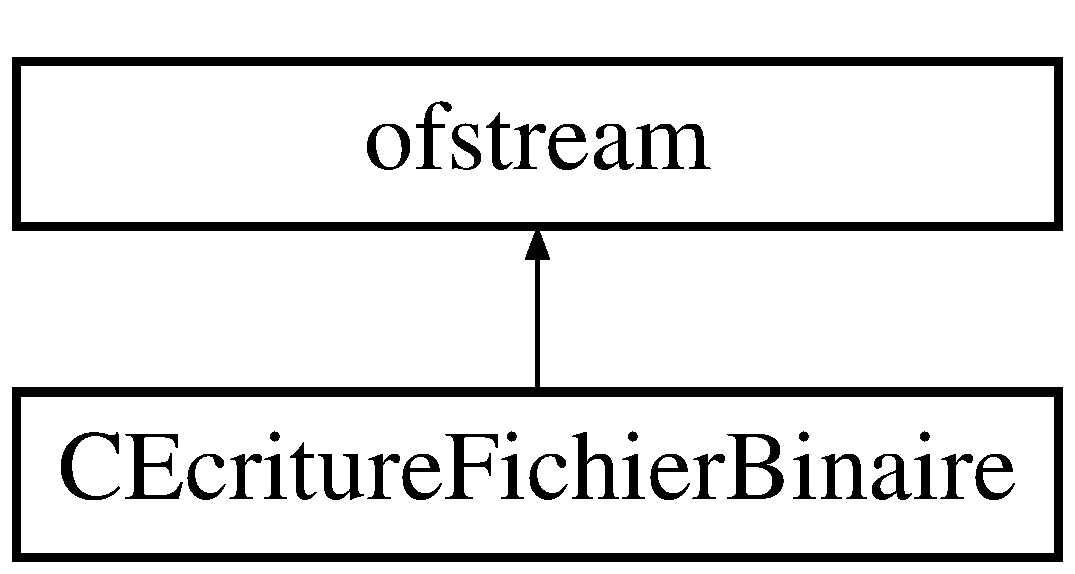
\includegraphics[height=2.000000cm]{class_c_ecriture_fichier_binaire}
\end{center}
\end{figure}
\subsection*{Public Member Functions}
\begin{DoxyCompactItemize}
\item 
\hyperlink{group__utilitaire_ga5b5846202001fecd71cd2a0afbbdb494}{C\+Ecriture\+Fichier\+Binaire} ()
\begin{DoxyCompactList}\small\item\em Constructeur par défaut. \end{DoxyCompactList}\item 
\hyperlink{group__utilitaire_gad19b9753aa12a9f25fd0febc3c899024}{C\+Ecriture\+Fichier\+Binaire} (const char $\ast$nom\+Fichier, openmode mode=std\+::ios\+::out$\vert$std\+::ios\+::binary)
\begin{DoxyCompactList}\small\item\em Constructeur par paramètre. \end{DoxyCompactList}\item 
void \hyperlink{group__utilitaire_ga7145545254c30909311d3b1ef0bdd07a}{null} (int n)
\begin{DoxyCompactList}\small\item\em Fonction pour insérer des caractères vides dans le fichier. \end{DoxyCompactList}\end{DoxyCompactItemize}
\subsection*{Friends}
\begin{DoxyCompactItemize}
\item 
\hypertarget{class_c_ecriture_fichier_binaire_a2c88c30ff08c7d9035596e0187d44e45}{}\hyperlink{class_c_ecriture_fichier_binaire}{C\+Ecriture\+Fichier\+Binaire} \& \hyperlink{class_c_ecriture_fichier_binaire_a2c88c30ff08c7d9035596e0187d44e45}{operator$<$} (\hyperlink{class_c_ecriture_fichier_binaire}{C\+Ecriture\+Fichier\+Binaire} \&out, const std\+::string \&s)\label{class_c_ecriture_fichier_binaire_a2c88c30ff08c7d9035596e0187d44e45}

\begin{DoxyCompactList}\small\item\em Surcharge de l\textquotesingle{}opérateur pour le type {\itshape std\+::string}. \end{DoxyCompactList}\item 
\hypertarget{class_c_ecriture_fichier_binaire_afcaa555d19b37490df9fda731cf8cb19}{}\hyperlink{class_c_ecriture_fichier_binaire}{C\+Ecriture\+Fichier\+Binaire} \& \hyperlink{class_c_ecriture_fichier_binaire_afcaa555d19b37490df9fda731cf8cb19}{operator$<$} (\hyperlink{class_c_ecriture_fichier_binaire}{C\+Ecriture\+Fichier\+Binaire} \&out, const double \&x)\label{class_c_ecriture_fichier_binaire_afcaa555d19b37490df9fda731cf8cb19}

\begin{DoxyCompactList}\small\item\em Surcharge de l\textquotesingle{}opérateur pour le type {\itshape double}. \end{DoxyCompactList}\item 
\hypertarget{class_c_ecriture_fichier_binaire_a68e43a125ee6c25828485dfb7270fdea}{}\hyperlink{class_c_ecriture_fichier_binaire}{C\+Ecriture\+Fichier\+Binaire} \& \hyperlink{class_c_ecriture_fichier_binaire_a68e43a125ee6c25828485dfb7270fdea}{operator$<$} (\hyperlink{class_c_ecriture_fichier_binaire}{C\+Ecriture\+Fichier\+Binaire} \&out, const float \&x)\label{class_c_ecriture_fichier_binaire_a68e43a125ee6c25828485dfb7270fdea}

\begin{DoxyCompactList}\small\item\em Surcharge de l\textquotesingle{}opérateur pour le type {\itshape float}. \end{DoxyCompactList}\item 
\hypertarget{class_c_ecriture_fichier_binaire_a57ac55aefec2f3dd683cef75c409944b}{}\hyperlink{class_c_ecriture_fichier_binaire}{C\+Ecriture\+Fichier\+Binaire} \& \hyperlink{class_c_ecriture_fichier_binaire_a57ac55aefec2f3dd683cef75c409944b}{operator$<$} (\hyperlink{class_c_ecriture_fichier_binaire}{C\+Ecriture\+Fichier\+Binaire} \&out, const int \&x)\label{class_c_ecriture_fichier_binaire_a57ac55aefec2f3dd683cef75c409944b}

\begin{DoxyCompactList}\small\item\em Surcharge de l\textquotesingle{}opérateur pour le type {\itshape int}. \end{DoxyCompactList}\item 
\hypertarget{class_c_ecriture_fichier_binaire_a38d0f050dcc8a79522b0fb9b9c591f72}{}\hyperlink{class_c_ecriture_fichier_binaire}{C\+Ecriture\+Fichier\+Binaire} \& \hyperlink{class_c_ecriture_fichier_binaire_a38d0f050dcc8a79522b0fb9b9c591f72}{operator$<$} (\hyperlink{class_c_ecriture_fichier_binaire}{C\+Ecriture\+Fichier\+Binaire} \&out, const unsigned int \&x)\label{class_c_ecriture_fichier_binaire_a38d0f050dcc8a79522b0fb9b9c591f72}

\begin{DoxyCompactList}\small\item\em Surcharge de l\textquotesingle{}opérateur pour le type {\itshape unsigned} {\itshape int}. \end{DoxyCompactList}\item 
\hypertarget{class_c_ecriture_fichier_binaire_a3cb25116e2558d967dfd21e812e47a3e}{}\hyperlink{class_c_ecriture_fichier_binaire}{C\+Ecriture\+Fichier\+Binaire} \& \hyperlink{class_c_ecriture_fichier_binaire_a3cb25116e2558d967dfd21e812e47a3e}{operator$<$} (\hyperlink{class_c_ecriture_fichier_binaire}{C\+Ecriture\+Fichier\+Binaire} \&out, const char \&x)\label{class_c_ecriture_fichier_binaire_a3cb25116e2558d967dfd21e812e47a3e}

\begin{DoxyCompactList}\small\item\em Surcharge de l\textquotesingle{}opérateur pour le type {\itshape char}. \end{DoxyCompactList}\item 
\hypertarget{class_c_ecriture_fichier_binaire_a37080aca11f391be69941db70093f77d}{}\hyperlink{class_c_ecriture_fichier_binaire}{C\+Ecriture\+Fichier\+Binaire} \& \hyperlink{class_c_ecriture_fichier_binaire_a37080aca11f391be69941db70093f77d}{operator$<$} (\hyperlink{class_c_ecriture_fichier_binaire}{C\+Ecriture\+Fichier\+Binaire} \&out, const bool \&x)\label{class_c_ecriture_fichier_binaire_a37080aca11f391be69941db70093f77d}

\begin{DoxyCompactList}\small\item\em Surcharge de l\textquotesingle{}opérateur pour le type {\itshape bool}. \end{DoxyCompactList}\end{DoxyCompactItemize}


\subsection{Detailed Description}
Cette classe contient des méthodes $<$ permettant d\textquotesingle{}écrire dans un fichier binaire des variables string, double, float, int, unsigned int, char, bool. 

\begin{DoxyAuthor}{Author}
D\+G\+I-\/2990 
\end{DoxyAuthor}
\begin{DoxyDate}{Date}
2005-\/10-\/15 
\end{DoxyDate}


The documentation for this class was generated from the following files\+:\begin{DoxyCompactItemize}
\item 
C\+:/\+Users/\+Louis/workspace/inf2990-\/01/\+Commun/\+Utilitaire/\hyperlink{_c_ecriture_fichier_binaire_8h}{C\+Ecriture\+Fichier\+Binaire.\+h}\item 
C\+:/\+Users/\+Louis/workspace/inf2990-\/01/\+Commun/\+Utilitaire/\hyperlink{_c_ecriture_fichier_binaire_8cpp}{C\+Ecriture\+Fichier\+Binaire.\+cpp}\end{DoxyCompactItemize}

\hypertarget{class_center_tool}{}\section{Center\+Tool Class Reference}
\label{class_center_tool}\index{Center\+Tool@{Center\+Tool}}


Classe concrète héritant de \hyperlink{class_tool}{Tool}, qui retourne le centre des objets sélectionnés.  




{\ttfamily \#include $<$Center\+Tool.\+h$>$}

Inheritance diagram for Center\+Tool\+:\begin{figure}[H]
\begin{center}
\leavevmode
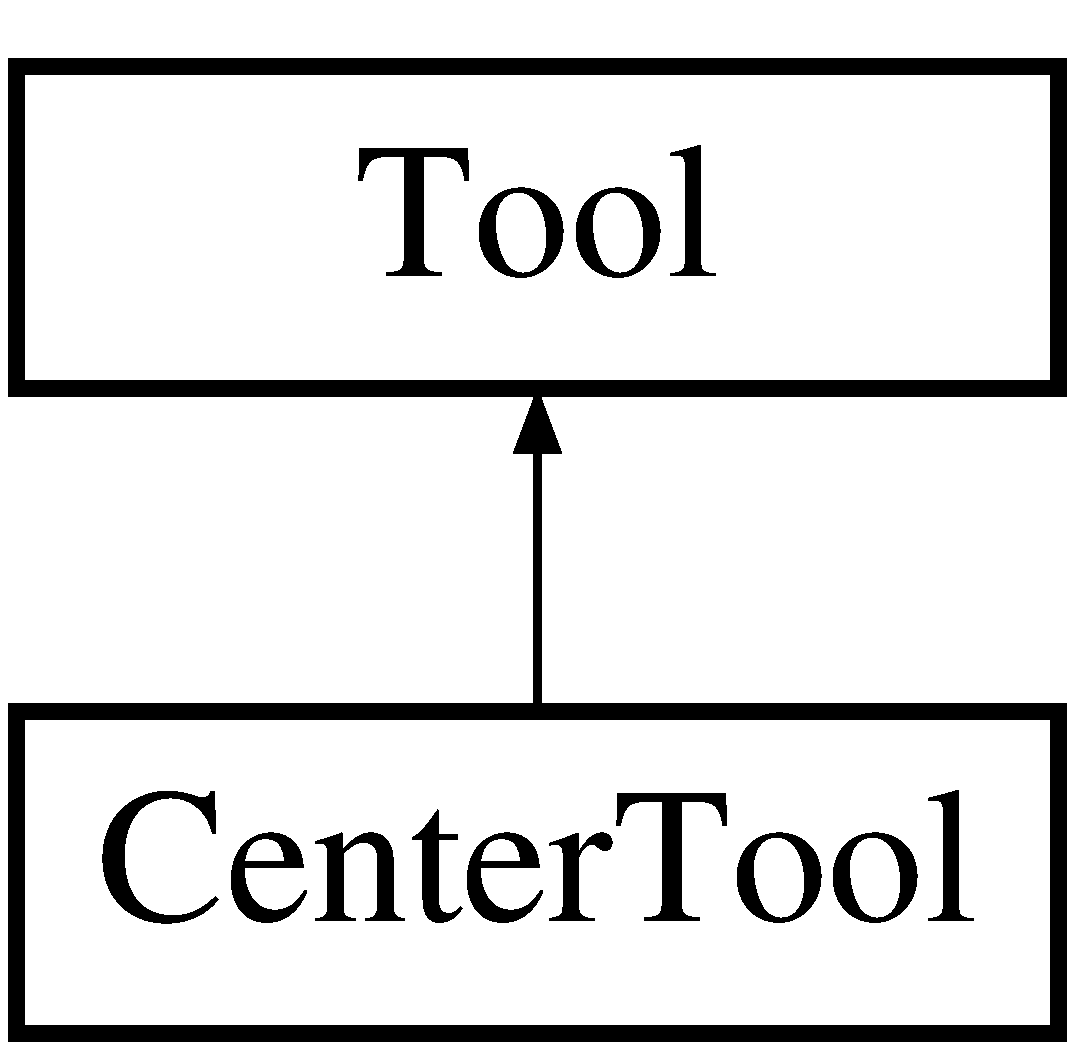
\includegraphics[height=2.000000cm]{class_center_tool}
\end{center}
\end{figure}
\subsection*{Public Member Functions}
\begin{DoxyCompactItemize}
\item 
\hyperlink{group__inf2990_ga3814d534b50e7dff7fbd7efef552685d}{Center\+Tool} ()
\item 
void \hyperlink{group__inf2990_ga9ceff880a444e12bc6b4dab4313c1809}{visit} (\hyperlink{class_noeud_cylindre}{Noeud\+Cylindre} $\ast$node) override
\item 
void \hyperlink{group__inf2990_ga8417547d629ccacfa218979e6ba6cdf5}{visit} (\hyperlink{class_noeud_depart}{Noeud\+Depart} $\ast$node) override
\item 
void \hyperlink{group__inf2990_gac441b1692c3b057050ced592ba372263}{visit} (\hyperlink{class_noeud_segment_concret}{Noeud\+Segment\+Concret} $\ast$node) override
\item 
void \hyperlink{group__inf2990_ga13d2bac067f4262be4fd60c302a07124}{visit} (\hyperlink{class_noeud_mur}{Noeud\+Mur} $\ast$node) override
\item 
glm\+::dvec3 \hyperlink{group__inf2990_gaf086e5f530c5189f4b72563a4abfe35f}{get\+Center} () const 
\begin{DoxyCompactList}\small\item\em Retourne le centre calculé \end{DoxyCompactList}\end{DoxyCompactItemize}
\subsection*{Protected Member Functions}
\begin{DoxyCompactItemize}
\item 
void \hyperlink{group__inf2990_gab64cc9d2d491c0bd04a1efc4756740df}{default\+Center} (\hyperlink{class_noeud_abstrait}{Noeud\+Abstrait} $\ast$node)
\begin{DoxyCompactList}\small\item\em Algorithme par défaut. \end{DoxyCompactList}\end{DoxyCompactItemize}


\subsection{Detailed Description}
Classe concrète héritant de \hyperlink{class_tool}{Tool}, qui retourne le centre des objets sélectionnés. 

\begin{DoxyAuthor}{Author}
I\+N\+F2990-\/\+A15-\/01 
\end{DoxyAuthor}
\begin{DoxyDate}{Date}
2015-\/09-\/25 
\end{DoxyDate}


The documentation for this class was generated from the following files\+:\begin{DoxyCompactItemize}
\item 
Sources/\+D\+L\+L/\+Application/\+Visitor/\hyperlink{_center_tool_8h}{Center\+Tool.\+h}\item 
Sources/\+D\+L\+L/\+Application/\+Visitor/\hyperlink{_center_tool_8cpp}{Center\+Tool.\+cpp}\end{DoxyCompactItemize}

\hypertarget{class_center_tool_test}{\section{Référence de la classe Center\-Tool\-Test}
\label{class_center_tool_test}\index{Center\-Tool\-Test@{Center\-Tool\-Test}}
}


Classe de test cppunit pour tester le bon fonctionnement des méthodes de la classe \hyperlink{class_center_tool}{Center\-Tool}.  




{\ttfamily \#include $<$Center\-Tool\-Test.\-h$>$}

Graphe d'héritage de Center\-Tool\-Test\-:\begin{figure}[H]
\begin{center}
\leavevmode
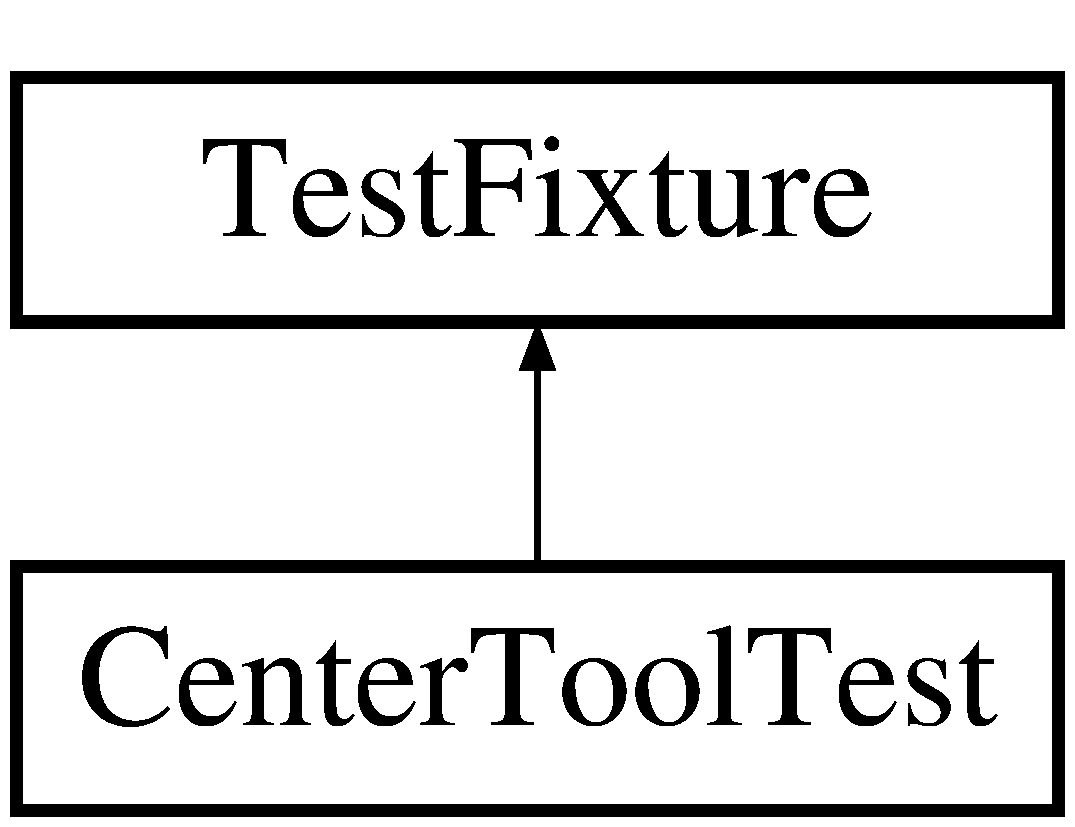
\includegraphics[height=2.000000cm]{class_center_tool_test}
\end{center}
\end{figure}
\subsection*{Fonctions membres publiques}
\begin{DoxyCompactItemize}
\item 
void \hyperlink{group__inf2990_gab5443e5a7c8e3ddcd5bac53be6663244}{set\-Up} ()
\begin{DoxyCompactList}\small\item\em Traitement à effectuer pour initialiser cette suite de tests. \end{DoxyCompactList}\item 
void \hyperlink{group__inf2990_ga837ac366aa728e8f9536e950b9da3769}{tear\-Down} ()
\begin{DoxyCompactList}\small\item\em Traitement à effectuer pour 'finaliser' cette suite de tests. \end{DoxyCompactList}\item 
void \hyperlink{group__inf2990_gab0e6197c88a207aacfd8e9d178a53a47}{test\-Center} ()
\begin{DoxyCompactList}\small\item\em Cas de test\-: centre géométrique de plusieurs objets. \end{DoxyCompactList}\end{DoxyCompactItemize}


\subsection{Description détaillée}
Classe de test cppunit pour tester le bon fonctionnement des méthodes de la classe \hyperlink{class_center_tool}{Center\-Tool}. 

\begin{DoxyAuthor}{Auteur}
I\-N\-F2990-\/\-A15-\/01 
\end{DoxyAuthor}
\begin{DoxyDate}{Date}
2015-\/11-\/09 
\end{DoxyDate}


La documentation de cette classe a été générée à partir des fichiers suivants \-:\begin{DoxyCompactItemize}
\item 
C\-:/\-Users/saron/\-Documents/inf2990-\/01/\-Sources/\-D\-L\-L/\-Tests/\hyperlink{_center_tool_test_8h}{Center\-Tool\-Test.\-h}\item 
C\-:/\-Users/saron/\-Documents/inf2990-\/01/\-Sources/\-D\-L\-L/\-Tests/\hyperlink{_center_tool_test_8cpp}{Center\-Tool\-Test.\-cpp}\end{DoxyCompactItemize}

\hypertarget{class_c_lecture_fichier_binaire}{\section{Référence de la classe C\-Lecture\-Fichier\-Binaire}
\label{class_c_lecture_fichier_binaire}\index{C\-Lecture\-Fichier\-Binaire@{C\-Lecture\-Fichier\-Binaire}}
}


cette classe contient des méthodes $>$ permettant de lire dans un fichier binaire des variables de types string, double, float, int, unsigned int, char, et bool.  




{\ttfamily \#include $<$C\-Lecture\-Fichier\-Binaire.\-h$>$}

Graphe d'héritage de C\-Lecture\-Fichier\-Binaire\-:\begin{figure}[H]
\begin{center}
\leavevmode
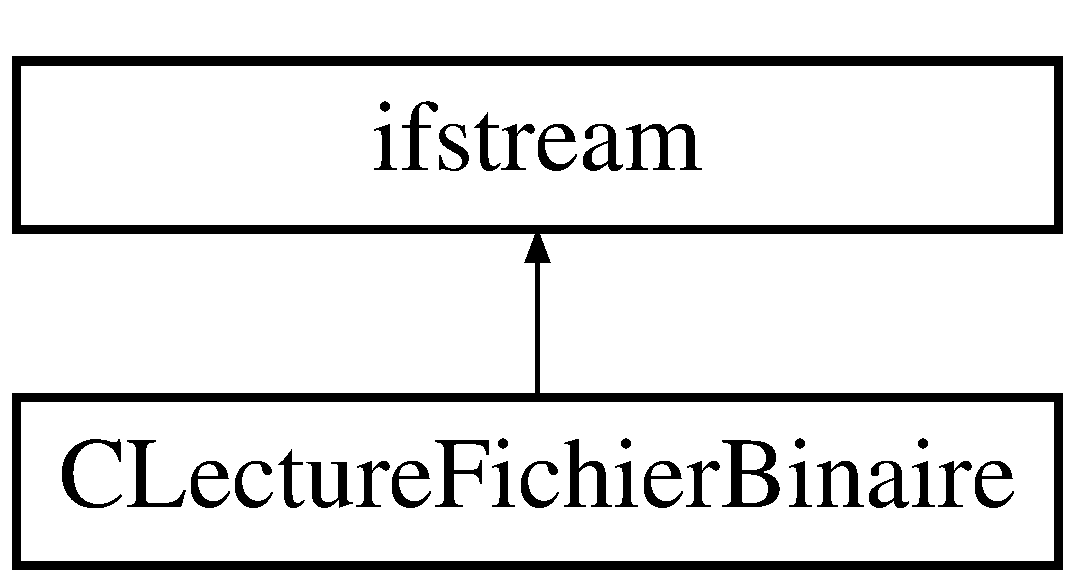
\includegraphics[height=2.000000cm]{class_c_lecture_fichier_binaire}
\end{center}
\end{figure}
\subsection*{Fonctions membres publiques}
\begin{DoxyCompactItemize}
\item 
\hyperlink{group__utilitaire_ga3a259905a2c14513846e6ecb8cf476ad}{C\-Lecture\-Fichier\-Binaire} ()
\begin{DoxyCompactList}\small\item\em Constructeur par défaut. \end{DoxyCompactList}\item 
\hyperlink{group__utilitaire_gac16ebab7b172408c2ba14605f61f0f84}{C\-Lecture\-Fichier\-Binaire} (const char $\ast$nom\-Fichier, openmode mode=std\-::ios\-::in$\vert$std\-::ios\-::binary)
\begin{DoxyCompactList}\small\item\em Constructeur par paramètre. \end{DoxyCompactList}\end{DoxyCompactItemize}
\subsection*{Amis}
\begin{DoxyCompactItemize}
\item 
\hypertarget{class_c_lecture_fichier_binaire_abc9f4d65dcf682dbf572f5110a00252d}{\hyperlink{class_c_lecture_fichier_binaire}{C\-Lecture\-Fichier\-Binaire} \& \hyperlink{class_c_lecture_fichier_binaire_abc9f4d65dcf682dbf572f5110a00252d}{operator$>$} (\hyperlink{class_c_lecture_fichier_binaire}{C\-Lecture\-Fichier\-Binaire} \&in, std\-::string \&s)}\label{class_c_lecture_fichier_binaire_abc9f4d65dcf682dbf572f5110a00252d}

\begin{DoxyCompactList}\small\item\em Surcharge de l'opérateur pour le type {\itshape std\-::string}. \end{DoxyCompactList}\item 
\hypertarget{class_c_lecture_fichier_binaire_a8b4123b210cccf9da0d2eb60dc19b8a0}{\hyperlink{class_c_lecture_fichier_binaire}{C\-Lecture\-Fichier\-Binaire} \& \hyperlink{class_c_lecture_fichier_binaire_a8b4123b210cccf9da0d2eb60dc19b8a0}{operator$>$} (\hyperlink{class_c_lecture_fichier_binaire}{C\-Lecture\-Fichier\-Binaire} \&in, double \&f)}\label{class_c_lecture_fichier_binaire_a8b4123b210cccf9da0d2eb60dc19b8a0}

\begin{DoxyCompactList}\small\item\em Surcharge de l'opérateur pour le type {\itshape double}. \end{DoxyCompactList}\item 
\hypertarget{class_c_lecture_fichier_binaire_a8727572665715de99f2908c711e45114}{\hyperlink{class_c_lecture_fichier_binaire}{C\-Lecture\-Fichier\-Binaire} \& \hyperlink{class_c_lecture_fichier_binaire_a8727572665715de99f2908c711e45114}{operator$>$} (\hyperlink{class_c_lecture_fichier_binaire}{C\-Lecture\-Fichier\-Binaire} \&in, float \&f)}\label{class_c_lecture_fichier_binaire_a8727572665715de99f2908c711e45114}

\begin{DoxyCompactList}\small\item\em Surcharge de l'opérateur pour le type {\itshape float}. \end{DoxyCompactList}\item 
\hypertarget{class_c_lecture_fichier_binaire_a327898e8bcb11d00bdb07e3e8bd361bd}{\hyperlink{class_c_lecture_fichier_binaire}{C\-Lecture\-Fichier\-Binaire} \& \hyperlink{class_c_lecture_fichier_binaire_a327898e8bcb11d00bdb07e3e8bd361bd}{operator$>$} (\hyperlink{class_c_lecture_fichier_binaire}{C\-Lecture\-Fichier\-Binaire} \&in, int \&f)}\label{class_c_lecture_fichier_binaire_a327898e8bcb11d00bdb07e3e8bd361bd}

\begin{DoxyCompactList}\small\item\em Surcharge de l'opérateur pour le type {\itshape int}. \end{DoxyCompactList}\item 
\hypertarget{class_c_lecture_fichier_binaire_a10555985d21e9277fd610554eb804ad4}{\hyperlink{class_c_lecture_fichier_binaire}{C\-Lecture\-Fichier\-Binaire} \& \hyperlink{class_c_lecture_fichier_binaire_a10555985d21e9277fd610554eb804ad4}{operator$>$} (\hyperlink{class_c_lecture_fichier_binaire}{C\-Lecture\-Fichier\-Binaire} \&in, unsigned int \&f)}\label{class_c_lecture_fichier_binaire_a10555985d21e9277fd610554eb804ad4}

\begin{DoxyCompactList}\small\item\em Surcharge de l'opérateur pour le type {\itshape unsigned} {\itshape int}. \end{DoxyCompactList}\item 
\hypertarget{class_c_lecture_fichier_binaire_a4a3ac4fa35e1f11664f6612d554d72bd}{\hyperlink{class_c_lecture_fichier_binaire}{C\-Lecture\-Fichier\-Binaire} \& \hyperlink{class_c_lecture_fichier_binaire_a4a3ac4fa35e1f11664f6612d554d72bd}{operator$>$} (\hyperlink{class_c_lecture_fichier_binaire}{C\-Lecture\-Fichier\-Binaire} \&in, char \&f)}\label{class_c_lecture_fichier_binaire_a4a3ac4fa35e1f11664f6612d554d72bd}

\begin{DoxyCompactList}\small\item\em Surcharge de l'opérateur pour le type {\itshape char}. \end{DoxyCompactList}\item 
\hypertarget{class_c_lecture_fichier_binaire_aaf7fbfa5e060c1e9015b0ffbd013f3e3}{\hyperlink{class_c_lecture_fichier_binaire}{C\-Lecture\-Fichier\-Binaire} \& \hyperlink{class_c_lecture_fichier_binaire_aaf7fbfa5e060c1e9015b0ffbd013f3e3}{operator$>$} (\hyperlink{class_c_lecture_fichier_binaire}{C\-Lecture\-Fichier\-Binaire} \&in, bool \&f)}\label{class_c_lecture_fichier_binaire_aaf7fbfa5e060c1e9015b0ffbd013f3e3}

\begin{DoxyCompactList}\small\item\em Surcharge de l'opérateur pour le type {\itshape bool}. \end{DoxyCompactList}\end{DoxyCompactItemize}


\subsection{Description détaillée}
cette classe contient des méthodes $>$ permettant de lire dans un fichier binaire des variables de types string, double, float, int, unsigned int, char, et bool. 

\begin{DoxyAuthor}{Auteur}
D\-G\-I-\/2990 
\end{DoxyAuthor}
\begin{DoxyDate}{Date}
2005-\/10-\/15 
\end{DoxyDate}


La documentation de cette classe a été générée à partir des fichiers suivants \-:\begin{DoxyCompactItemize}
\item 
C\-:/\-Users/saron/\-Documents/inf2990-\/01/\-Commun/\-Utilitaire/\hyperlink{_c_lecture_fichier_binaire_8h}{C\-Lecture\-Fichier\-Binaire.\-h}\item 
C\-:/\-Users/saron/\-Documents/inf2990-\/01/\-Commun/\-Utilitaire/\hyperlink{_c_lecture_fichier_binaire_8cpp}{C\-Lecture\-Fichier\-Binaire.\-cpp}\end{DoxyCompactItemize}

\hypertarget{class_collision_tool}{\section{Référence de la classe Collision\-Tool}
\label{class_collision_tool}\index{Collision\-Tool@{Collision\-Tool}}
}


Classe concrète héritant de \hyperlink{class_tool}{Tool}, qui effectue l'opération d'enregistrement de l'angle sur un noeud de l'arbre de rendu.  




{\ttfamily \#include $<$Collision\-Tool.\-h$>$}

Graphe d'héritage de Collision\-Tool\-:\begin{figure}[H]
\begin{center}
\leavevmode
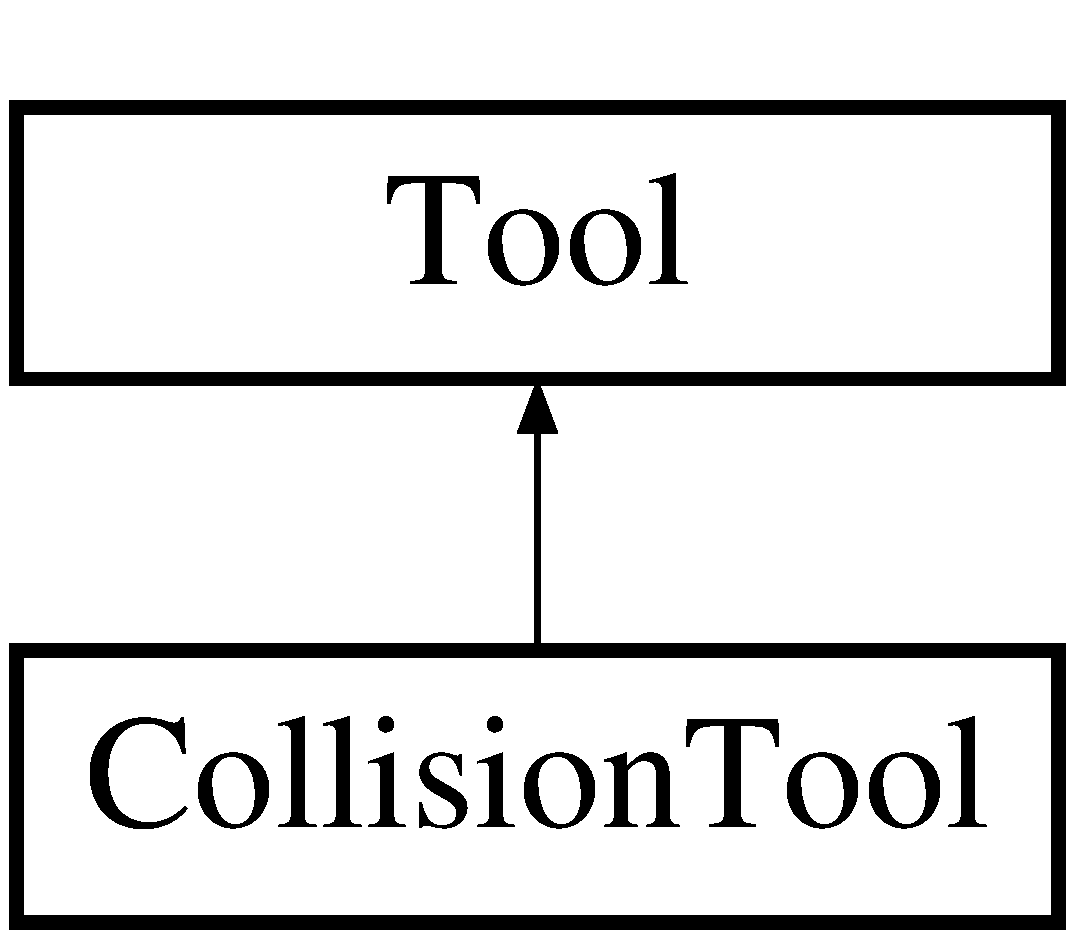
\includegraphics[height=2.000000cm]{class_collision_tool}
\end{center}
\end{figure}
\subsection*{Fonctions membres publiques}
\begin{DoxyCompactItemize}
\item 
\hyperlink{group__inf2990_ga2f19aaeb96c50199582fbd6146a22505}{Collision\-Tool} (\hyperlink{class_noeud_robot}{Noeud\-Robot} $\ast$robot)
\item 
void \hyperlink{group__inf2990_gaeabc2a2158a27714c8db5c076fe40720}{visit} (\hyperlink{class_noeud_cylindre}{Noeud\-Cylindre} $\ast$node) override
\item 
\hypertarget{class_collision_tool_a899bce8343b9fd961a525f4b9b70501f}{void {\bfseries visit} (\hyperlink{class_noeud_depart}{Noeud\-Depart} $\ast$node) override}\label{class_collision_tool_a899bce8343b9fd961a525f4b9b70501f}

\item 
\hypertarget{class_collision_tool_a7a7d8fe3caee1571a307190b9be35e7b}{void {\bfseries visit} (\hyperlink{class_noeud_segment_concret}{Noeud\-Segment\-Concret} $\ast$node) override}\label{class_collision_tool_a7a7d8fe3caee1571a307190b9be35e7b}

\item 
void \hyperlink{group__inf2990_ga25177ba7c7bb3179b850f4b702906b38}{visit} (\hyperlink{class_noeud_mur}{Noeud\-Mur} $\ast$node) override
\end{DoxyCompactItemize}
\subsection*{Fonctions membres publiques statiques}
\begin{DoxyCompactItemize}
\item 
static void \hyperlink{group__inf2990_gabf47107895dd5a494323f678fd430385}{rotate} (glm\-::dvec3 \&point, double angle, const glm\-::dvec3 \&center)
\item 
static double \hyperlink{group__inf2990_gacde31d7d23d078dae0286e8f3088bb32}{length} (glm\-::dvec3 vect)
\end{DoxyCompactItemize}


\subsection{Description détaillée}
Classe concrète héritant de \hyperlink{class_tool}{Tool}, qui effectue l'opération d'enregistrement de l'angle sur un noeud de l'arbre de rendu. 

\begin{DoxyAuthor}{Auteur}
I\-N\-F2990-\/\-A15-\/01 
\end{DoxyAuthor}
\begin{DoxyDate}{Date}
2015-\/10-\/21 
\end{DoxyDate}


La documentation de cette classe a été générée à partir des fichiers suivants \-:\begin{DoxyCompactItemize}
\item 
C\-:/\-Users/saron/\-Documents/inf2990-\/01/\-Sources/\-D\-L\-L/\-Application/\-Visitor/\hyperlink{_collision_tool_8h}{Collision\-Tool.\-h}\item 
C\-:/\-Users/saron/\-Documents/inf2990-\/01/\-Sources/\-D\-L\-L/\-Application/\-Visitor/\hyperlink{_collision_tool_8cpp}{Collision\-Tool.\-cpp}\end{DoxyCompactItemize}

\hypertarget{class_collision_tool_test}{\section{Référence de la classe Collision\-Tool\-Test}
\label{class_collision_tool_test}\index{Collision\-Tool\-Test@{Collision\-Tool\-Test}}
}


Classe de test cppunit pour tester le bon fonctionnement des méthodes de la classe \hyperlink{class_collision_tool}{Collision\-Tool}.  




{\ttfamily \#include $<$Collision\-Tool\-Test.\-h$>$}

Graphe d'héritage de Collision\-Tool\-Test\-:\begin{figure}[H]
\begin{center}
\leavevmode
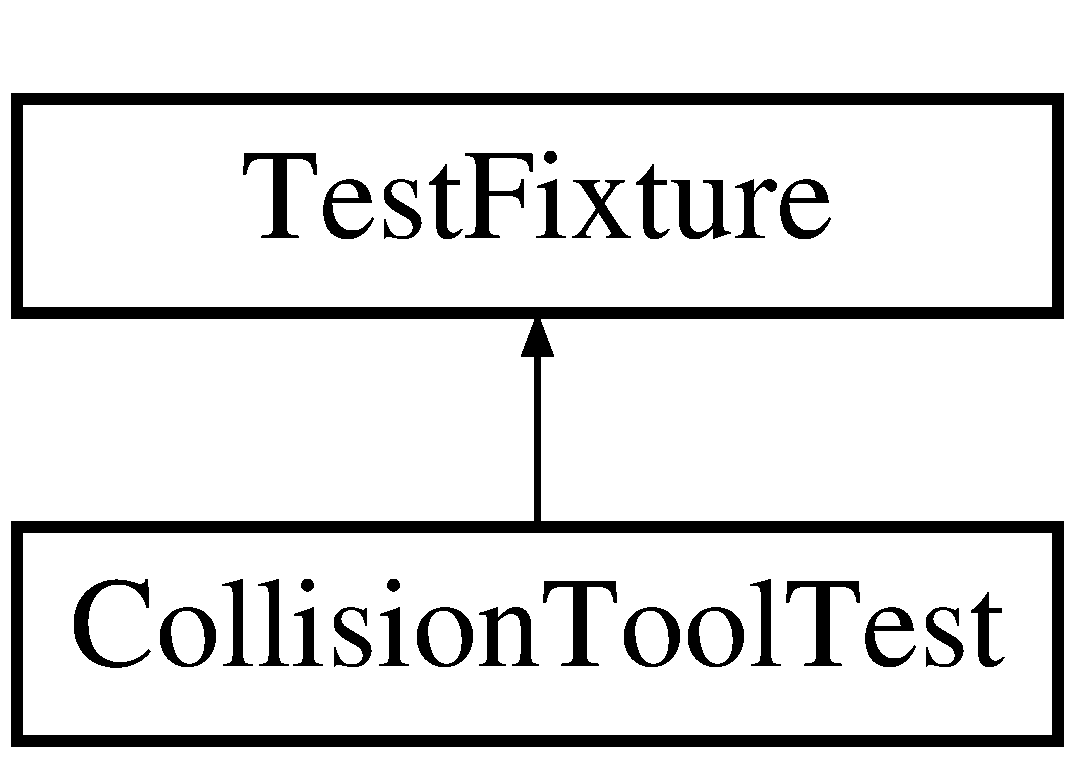
\includegraphics[height=2.000000cm]{class_collision_tool_test}
\end{center}
\end{figure}
\subsection*{Fonctions membres publiques}
\begin{DoxyCompactItemize}
\item 
void \hyperlink{group__inf2990_ga6924da693899b253751b489928bd5e04}{set\-Up} ()
\begin{DoxyCompactList}\small\item\em Traitement à effectuer pour initialiser cette suite de tests. \end{DoxyCompactList}\item 
void \hyperlink{group__inf2990_gae8e5960d925ec082674afdd45e7ea368}{tear\-Down} ()
\begin{DoxyCompactList}\small\item\em Traitement à effectuer pour 'finaliser' cette suite de tests. \end{DoxyCompactList}\item 
void \hyperlink{group__inf2990_gabd062c4f55b2f09df44c6defd20bea7f}{test\-Rotate} ()
\begin{DoxyCompactList}\small\item\em Cas de test\-: rotation d'un point autour d'un autre. \end{DoxyCompactList}\item 
void \hyperlink{group__inf2990_ga0951a401c6a0fb9bdd17c990827e6d57}{test\-Length} ()
\begin{DoxyCompactList}\small\item\em Cas de test\-: longueur d'un vecteur. \end{DoxyCompactList}\end{DoxyCompactItemize}


\subsection{Description détaillée}
Classe de test cppunit pour tester le bon fonctionnement des méthodes de la classe \hyperlink{class_collision_tool}{Collision\-Tool}. 

\begin{DoxyAuthor}{Auteur}
I\-N\-F2990-\/\-A15-\/01 
\end{DoxyAuthor}
\begin{DoxyDate}{Date}
2015-\/11-\/06 
\end{DoxyDate}


La documentation de cette classe a été générée à partir des fichiers suivants \-:\begin{DoxyCompactItemize}
\item 
C\-:/\-Users/saron/\-Documents/inf2990-\/01/\-Sources/\-D\-L\-L/\-Tests/\hyperlink{_collision_tool_test_8h}{Collision\-Tool\-Test.\-h}\item 
C\-:/\-Users/saron/\-Documents/inf2990-\/01/\-Sources/\-D\-L\-L/\-Tests/\hyperlink{_collision_tool_test_8cpp}{Collision\-Tool\-Test.\-cpp}\end{DoxyCompactItemize}

\hypertarget{classutilitaire_1_1_compteur_affichage}{\section{Référence de la classe utilitaire\-:\-:Compteur\-Affichage}
\label{classutilitaire_1_1_compteur_affichage}\index{utilitaire\-::\-Compteur\-Affichage@{utilitaire\-::\-Compteur\-Affichage}}
}


Classe qui gère le compte des affichages par secondes (\char`\"{}\-F\-P\-S\char`\"{}).  




{\ttfamily \#include $<$Compteur\-Affichage.\-h$>$}

\subsection*{Fonctions membres publiques}
\begin{DoxyCompactItemize}
\item 
int \hyperlink{classutilitaire_1_1_compteur_affichage_a1902a495b4898b3f7ab9056537db00cc}{obtenir\-Affichages\-Seconde} () const 
\begin{DoxyCompactList}\small\item\em Obtient le dernier nombre calculé d'affichages par seconde. \end{DoxyCompactList}\item 
void \hyperlink{classutilitaire_1_1_compteur_affichage_a49f6562d1a37e275ff8c8c0e9be41ab5}{signaler\-Affichage} ()
\begin{DoxyCompactList}\small\item\em Indique qu'un affichage vient de se produire. \end{DoxyCompactList}\item 
void \hyperlink{classutilitaire_1_1_compteur_affichage_a69b89a3d76cde700f1c08580bab010ca}{reinitialiser} ()
\begin{DoxyCompactList}\small\item\em Réinitialise le compteur d'affichage. \end{DoxyCompactList}\end{DoxyCompactItemize}
\subsection*{Fonctions membres publiques statiques}
\begin{DoxyCompactItemize}
\item 
static \hyperlink{classutilitaire_1_1_compteur_affichage}{Compteur\-Affichage} $\ast$ \hyperlink{classutilitaire_1_1_compteur_affichage_a87a0785c0c73f0da0f6ffc4a86a609fe}{obtenir\-Instance} ()
\begin{DoxyCompactList}\small\item\em Obtient l'instance unique de la classe. \end{DoxyCompactList}\item 
static void \hyperlink{classutilitaire_1_1_compteur_affichage_ae37d88f73c83bfd3ff3c95496c9ef400}{liberer\-Instance} ()
\begin{DoxyCompactList}\small\item\em Libère l'instance unique de la classe. \end{DoxyCompactList}\end{DoxyCompactItemize}


\subsection{Description détaillée}
Classe qui gère le compte des affichages par secondes (\char`\"{}\-F\-P\-S\char`\"{}). 

\begin{DoxyAuthor}{Auteur}
Martin Bisson 
\end{DoxyAuthor}
\begin{DoxyDate}{Date}
2007-\/03-\/09 
\end{DoxyDate}


\subsection{Documentation des fonctions membres}
\hypertarget{classutilitaire_1_1_compteur_affichage_ae37d88f73c83bfd3ff3c95496c9ef400}{\index{utilitaire\-::\-Compteur\-Affichage@{utilitaire\-::\-Compteur\-Affichage}!liberer\-Instance@{liberer\-Instance}}
\index{liberer\-Instance@{liberer\-Instance}!utilitaire::CompteurAffichage@{utilitaire\-::\-Compteur\-Affichage}}
\subsubsection[{liberer\-Instance}]{\setlength{\rightskip}{0pt plus 5cm}void utilitaire\-::\-Compteur\-Affichage\-::liberer\-Instance (
\begin{DoxyParamCaption}
{}
\end{DoxyParamCaption}
)\hspace{0.3cm}{\ttfamily [static]}}}\label{classutilitaire_1_1_compteur_affichage_ae37d88f73c83bfd3ff3c95496c9ef400}


Libère l'instance unique de la classe. 

Cette fonction libère l'instance unique de cette classe.

\begin{DoxyReturn}{Renvoie}
Aucune. 
\end{DoxyReturn}
\hypertarget{classutilitaire_1_1_compteur_affichage_a1902a495b4898b3f7ab9056537db00cc}{\index{utilitaire\-::\-Compteur\-Affichage@{utilitaire\-::\-Compteur\-Affichage}!obtenir\-Affichages\-Seconde@{obtenir\-Affichages\-Seconde}}
\index{obtenir\-Affichages\-Seconde@{obtenir\-Affichages\-Seconde}!utilitaire::CompteurAffichage@{utilitaire\-::\-Compteur\-Affichage}}
\subsubsection[{obtenir\-Affichages\-Seconde}]{\setlength{\rightskip}{0pt plus 5cm}int utilitaire\-::\-Compteur\-Affichage\-::obtenir\-Affichages\-Seconde (
\begin{DoxyParamCaption}
{}
\end{DoxyParamCaption}
) const\hspace{0.3cm}{\ttfamily [inline]}}}\label{classutilitaire_1_1_compteur_affichage_a1902a495b4898b3f7ab9056537db00cc}


Obtient le dernier nombre calculé d'affichages par seconde. 

Cette fonction retourne le dernier nombre d'affichages par seconde calculé par le compteur.

\begin{DoxyReturn}{Renvoie}
Le nombre d'affichages par seconce le plus récent. 
\end{DoxyReturn}
\hypertarget{classutilitaire_1_1_compteur_affichage_a87a0785c0c73f0da0f6ffc4a86a609fe}{\index{utilitaire\-::\-Compteur\-Affichage@{utilitaire\-::\-Compteur\-Affichage}!obtenir\-Instance@{obtenir\-Instance}}
\index{obtenir\-Instance@{obtenir\-Instance}!utilitaire::CompteurAffichage@{utilitaire\-::\-Compteur\-Affichage}}
\subsubsection[{obtenir\-Instance}]{\setlength{\rightskip}{0pt plus 5cm}{\bf Compteur\-Affichage} $\ast$ utilitaire\-::\-Compteur\-Affichage\-::obtenir\-Instance (
\begin{DoxyParamCaption}
{}
\end{DoxyParamCaption}
)\hspace{0.3cm}{\ttfamily [static]}}}\label{classutilitaire_1_1_compteur_affichage_a87a0785c0c73f0da0f6ffc4a86a609fe}


Obtient l'instance unique de la classe. 

Cette fonction retourne un pointeur vers l'instance unique de la classe. Si cette instance n'a pas été créée, elle la crée. Cette création n'est toutefois pas nécessairement \char`\"{}thread-\/safe\char`\"{}, car aucun verrou n'est pris entre le test pour savoir si l'instance existe et le moment de sa création.

\begin{DoxyReturn}{Renvoie}
Un pointeur vers l'instance unique de cette classe. 
\end{DoxyReturn}
\hypertarget{classutilitaire_1_1_compteur_affichage_a69b89a3d76cde700f1c08580bab010ca}{\index{utilitaire\-::\-Compteur\-Affichage@{utilitaire\-::\-Compteur\-Affichage}!reinitialiser@{reinitialiser}}
\index{reinitialiser@{reinitialiser}!utilitaire::CompteurAffichage@{utilitaire\-::\-Compteur\-Affichage}}
\subsubsection[{reinitialiser}]{\setlength{\rightskip}{0pt plus 5cm}void utilitaire\-::\-Compteur\-Affichage\-::reinitialiser (
\begin{DoxyParamCaption}
{}
\end{DoxyParamCaption}
)}}\label{classutilitaire_1_1_compteur_affichage_a69b89a3d76cde700f1c08580bab010ca}


Réinitialise le compteur d'affichage. 

Cette fonction réinitialise le compteur d'affichage à son état initiale.

\begin{DoxyReturn}{Renvoie}
Aucune. 
\end{DoxyReturn}
\hypertarget{classutilitaire_1_1_compteur_affichage_a49f6562d1a37e275ff8c8c0e9be41ab5}{\index{utilitaire\-::\-Compteur\-Affichage@{utilitaire\-::\-Compteur\-Affichage}!signaler\-Affichage@{signaler\-Affichage}}
\index{signaler\-Affichage@{signaler\-Affichage}!utilitaire::CompteurAffichage@{utilitaire\-::\-Compteur\-Affichage}}
\subsubsection[{signaler\-Affichage}]{\setlength{\rightskip}{0pt plus 5cm}void utilitaire\-::\-Compteur\-Affichage\-::signaler\-Affichage (
\begin{DoxyParamCaption}
{}
\end{DoxyParamCaption}
)}}\label{classutilitaire_1_1_compteur_affichage_a49f6562d1a37e275ff8c8c0e9be41ab5}


Indique qu'un affichage vient de se produire. 

Cette fonction effectue le traitement nécessaire lorsqu'un affichage est signalée, c'est-\/à-\/dire qu'elle incrémente le compte et vérifie si la limite de temps pour la mise à jour est dépassée.

\begin{DoxyReturn}{Renvoie}
Aucune. 
\end{DoxyReturn}


La documentation de cette classe a été générée à partir des fichiers suivants \-:\begin{DoxyCompactItemize}
\item 
C\-:/\-Users/saron/\-Documents/inf2990-\/01/\-Commun/\-Utilitaire/\hyperlink{_compteur_affichage_8h}{Compteur\-Affichage.\-h}\item 
C\-:/\-Users/saron/\-Documents/inf2990-\/01/\-Commun/\-Utilitaire/\hyperlink{_compteur_affichage_8cpp}{Compteur\-Affichage.\-cpp}\end{DoxyCompactItemize}

\hypertarget{class_interface_graphique_1_1_config_panel}{\section{Référence de la classe Interface\-Graphique.\-Config\-Panel}
\label{class_interface_graphique_1_1_config_panel}\index{Interface\-Graphique.\-Config\-Panel@{Interface\-Graphique.\-Config\-Panel}}
}


Interaction logic for Config\-Panel.\-xaml  


Graphe d'héritage de Interface\-Graphique.\-Config\-Panel\-:\begin{figure}[H]
\begin{center}
\leavevmode
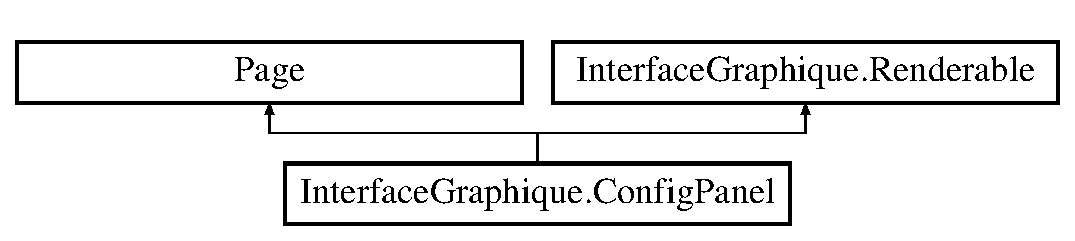
\includegraphics[height=2.000000cm]{class_interface_graphique_1_1_config_panel}
\end{center}
\end{figure}
\subsection*{Fonctions membres publiques}
\begin{DoxyCompactItemize}
\item 
\hypertarget{class_interface_graphique_1_1_config_panel_ad4304d5a2f0476206ed7032aafcc0c8b}{delegate void {\bfseries Click\-Event\-Handler} (object sender, Event\-Args e)}\label{class_interface_graphique_1_1_config_panel_ad4304d5a2f0476206ed7032aafcc0c8b}

\item 
\hypertarget{class_interface_graphique_1_1_config_panel_a07483b31c963861c00ad56693a1869da}{void {\bfseries Frame\-Update} (double time)}\label{class_interface_graphique_1_1_config_panel_a07483b31c963861c00ad56693a1869da}

\item 
\hypertarget{class_interface_graphique_1_1_config_panel_a80c2d11adae87e83b29f801fcb267756}{void {\bfseries Profile\-Property\-Changes} (object o, Event\-Args e)}\label{class_interface_graphique_1_1_config_panel_a80c2d11adae87e83b29f801fcb267756}

\end{DoxyCompactItemize}
\subsection*{Attributs publics}
\begin{DoxyCompactItemize}
\item 
\hypertarget{class_interface_graphique_1_1_config_panel_a65e81ecd1c7584257fda71c8c382ebdb}{\hyperlink{class_interface_graphique_1_1_profil}{Profil} {\bfseries Selected\-Item}}\label{class_interface_graphique_1_1_config_panel_a65e81ecd1c7584257fda71c8c382ebdb}

\item 
\hypertarget{class_interface_graphique_1_1_config_panel_a1965af1378c44678db40ee365c5bebd0}{bool {\bfseries is\-Profile\-Form\-Enabled} = true}\label{class_interface_graphique_1_1_config_panel_a1965af1378c44678db40ee365c5bebd0}

\item 
\hypertarget{class_interface_graphique_1_1_config_panel_a672032385e973ce332d986e3d3ed42d7}{\hyperlink{class_interface_graphique_1_1_key_bindings}{Key\-Bindings} {\bfseries keybindings}}\label{class_interface_graphique_1_1_config_panel_a672032385e973ce332d986e3d3ed42d7}

\item 
\hypertarget{class_interface_graphique_1_1_config_panel_a611b859778d97914289ba09523a208e6}{\hyperlink{class_interface_graphique_1_1_settings}{Settings} {\bfseries settings}}\label{class_interface_graphique_1_1_config_panel_a611b859778d97914289ba09523a208e6}

\end{DoxyCompactItemize}
\subsection*{Événements}
\begin{DoxyCompactItemize}
\item 
\hypertarget{class_interface_graphique_1_1_config_panel_a17fac5244e6f1acf42259e796b55de6b}{Click\-Event\-Handler {\bfseries Load\-Main\-Menu}}\label{class_interface_graphique_1_1_config_panel_a17fac5244e6f1acf42259e796b55de6b}

\end{DoxyCompactItemize}


\subsection{Description détaillée}
Interaction logic for Config\-Panel.\-xaml 



La documentation de cette classe a été générée à partir du fichier suivant \-:\begin{DoxyCompactItemize}
\item 
C\-:/\-Users/saron/\-Documents/inf2990-\/01/\-Sources/\-Interface\-Graphique/Config\-Panel.\-xaml.\-cs\end{DoxyCompactItemize}

\hypertarget{class_interface_graphique_1_1_config_panel_data}{\section{Référence de la classe Interface\-Graphique.\-Config\-Panel\-Data}
\label{class_interface_graphique_1_1_config_panel_data}\index{Interface\-Graphique.\-Config\-Panel\-Data@{Interface\-Graphique.\-Config\-Panel\-Data}}
}
\subsection*{Fonctions membres publiques}
\begin{DoxyCompactItemize}
\item 
\hypertarget{class_interface_graphique_1_1_config_panel_data_abe79b5dc9ab2bf3acdc061442c002d27}{\hyperlink{class_interface_graphique_1_1_settings}{Settings} {\bfseries Load\-Settings} ()}\label{class_interface_graphique_1_1_config_panel_data_abe79b5dc9ab2bf3acdc061442c002d27}

\item 
\hypertarget{class_interface_graphique_1_1_config_panel_data_aea03392dee9190d4a1bade4fb7f2a909}{void {\bfseries Save\-Settings} (\hyperlink{class_interface_graphique_1_1_settings}{Settings} settings)}\label{class_interface_graphique_1_1_config_panel_data_aea03392dee9190d4a1bade4fb7f2a909}

\item 
\hypertarget{class_interface_graphique_1_1_config_panel_data_aac0027068cb2b782ccd0131adfee2dab}{\hyperlink{class_interface_graphique_1_1_key_bindings}{Key\-Bindings} {\bfseries Load\-Keybindings} ()}\label{class_interface_graphique_1_1_config_panel_data_aac0027068cb2b782ccd0131adfee2dab}

\item 
\hypertarget{class_interface_graphique_1_1_config_panel_data_a648cccdcb7afff19ce562792ed64976e}{void {\bfseries Save\-Keybindings} (\hyperlink{class_interface_graphique_1_1_key_bindings}{Key\-Bindings} keys)}\label{class_interface_graphique_1_1_config_panel_data_a648cccdcb7afff19ce562792ed64976e}

\item 
\hypertarget{class_interface_graphique_1_1_config_panel_data_af1303250bbfe56eda9c920ec42a590b8}{void {\bfseries Save\-Profiles} (List$<$ \hyperlink{class_interface_graphique_1_1_profil}{Profil} $>$ profiles)}\label{class_interface_graphique_1_1_config_panel_data_af1303250bbfe56eda9c920ec42a590b8}

\item 
\hypertarget{class_interface_graphique_1_1_config_panel_data_a04d1f1d54f539135c91891281411f4cf}{List$<$ \hyperlink{class_interface_graphique_1_1_profil}{Profil} $>$ {\bfseries Load\-Profiles} ()}\label{class_interface_graphique_1_1_config_panel_data_a04d1f1d54f539135c91891281411f4cf}

\end{DoxyCompactItemize}


La documentation de cette classe a été générée à partir du fichier suivant \-:\begin{DoxyCompactItemize}
\item 
C\-:/\-Users/saron/\-Documents/inf2990-\/01/\-Sources/\-Interface\-Graphique/Config\-Panel\-Data.\-cs\end{DoxyCompactItemize}

\hypertarget{class_config_scene}{}\section{Config\+Scene Class Reference}
\label{class_config_scene}\index{Config\+Scene@{Config\+Scene}}


Les variables de configuration de la classe C\+Scene. C\textquotesingle{}est une classe singleton.  




{\ttfamily \#include $<$Config\+Scene.\+h$>$}

Inheritance diagram for Config\+Scene\+:\begin{figure}[H]
\begin{center}
\leavevmode
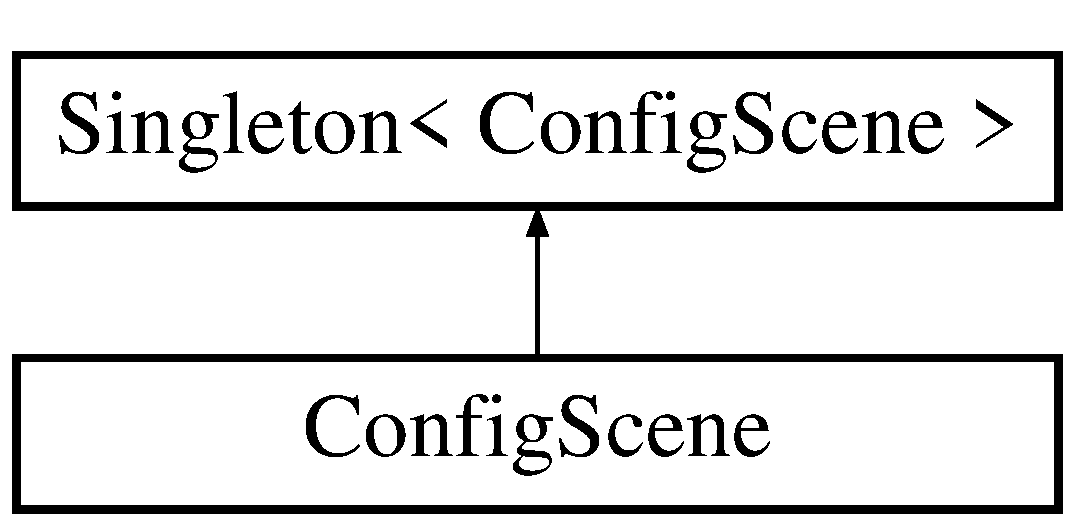
\includegraphics[height=2.000000cm]{class_config_scene}
\end{center}
\end{figure}
\subsection*{Public Member Functions}
\begin{DoxyCompactItemize}
\item 
void \hyperlink{group__inf2990_ga3d0152df0c8c134ecd1a1741302db839}{creer\+D\+O\+M} (tinyxml2\+::\+X\+M\+L\+Document \&document) const 
\begin{DoxyCompactList}\small\item\em Créer le D\+O\+M avec les valeurs. \end{DoxyCompactList}\item 
void \hyperlink{group__inf2990_gaeacd60be947ce76a1302f6bbb40c90b1}{lire\+D\+O\+M} (tinyxml2\+::\+X\+M\+L\+Document const \&document)
\begin{DoxyCompactList}\small\item\em Lire les valeurs du D\+O\+M. \end{DoxyCompactList}\end{DoxyCompactItemize}
\subsection*{Static Public Attributes}
\begin{DoxyCompactItemize}
\item 
\hypertarget{group__inf2990_gadb487b450a0314a5d1f75cf31ce502eb}{}static int \hyperlink{group__inf2990_gadb487b450a0314a5d1f75cf31ce502eb}{C\+A\+L\+C\+U\+L\+S\+\_\+\+P\+A\+R\+\_\+\+I\+M\+A\+G\+E} \{ 50 \}\label{group__inf2990_gadb487b450a0314a5d1f75cf31ce502eb}

\begin{DoxyCompactList}\small\item\em Nombre de calculs par image. \end{DoxyCompactList}\end{DoxyCompactItemize}
\subsection*{Additional Inherited Members}


\subsection{Detailed Description}
Les variables de configuration de la classe C\+Scene. C\textquotesingle{}est une classe singleton. 

\begin{DoxyAuthor}{Author}
Jean-\/\+François Pérusse 
\end{DoxyAuthor}
\begin{DoxyDate}{Date}
2007-\/01-\/10 
\end{DoxyDate}


The documentation for this class was generated from the following files\+:\begin{DoxyCompactItemize}
\item 
Sources/\+D\+L\+L/\+Configuration/\hyperlink{_config_scene_8h}{Config\+Scene.\+h}\item 
Sources/\+D\+L\+L/\+Configuration/\hyperlink{_config_scene_8cpp}{Config\+Scene.\+cpp}\end{DoxyCompactItemize}

\hypertarget{class_config_scene_test}{\section{Référence de la classe Config\-Scene\-Test}
\label{class_config_scene_test}\index{Config\-Scene\-Test@{Config\-Scene\-Test}}
}


Classe de test cppunit pour tester le bon fonctionnement des méthodes de la classe \hyperlink{class_config_scene}{Config\-Scene}.  




{\ttfamily \#include $<$Config\-Scene\-Test.\-h$>$}

Graphe d'héritage de Config\-Scene\-Test\-:\begin{figure}[H]
\begin{center}
\leavevmode
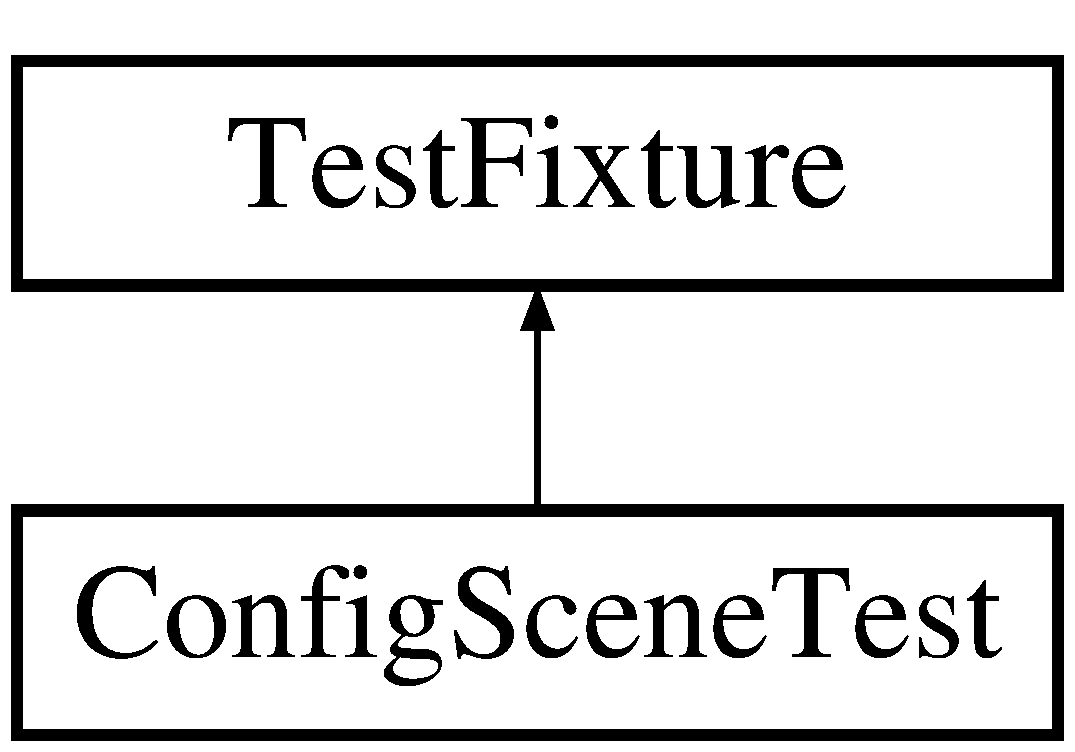
\includegraphics[height=2.000000cm]{class_config_scene_test}
\end{center}
\end{figure}
\subsection*{Fonctions membres publiques}
\begin{DoxyCompactItemize}
\item 
void \hyperlink{group__inf2990_ga707d7400843047e67b736ab79bafb5a0}{set\-Up} ()
\begin{DoxyCompactList}\small\item\em Traitement à effectuer pour initialiser cette suite de tests. \end{DoxyCompactList}\item 
void \hyperlink{group__inf2990_ga889ed3891c3e55280cabb982953906d9}{tear\-Down} ()
\begin{DoxyCompactList}\small\item\em Traitement à effectuer pour 'finaliser' cette suite de tests. \end{DoxyCompactList}\item 
void \hyperlink{group__inf2990_ga0f09d52bc30d87f18b0341e1052efb74}{test\-Sauvegarde\-Chargement} ()
\begin{DoxyCompactList}\small\item\em Cas de test\-: sauvegarde et chargement X\-M\-L de la configuration. \end{DoxyCompactList}\end{DoxyCompactItemize}


\subsection{Description détaillée}
Classe de test cppunit pour tester le bon fonctionnement des méthodes de la classe \hyperlink{class_config_scene}{Config\-Scene}. 

\begin{DoxyAuthor}{Auteur}
Julien Gascon-\/\-Samson 
\end{DoxyAuthor}
\begin{DoxyDate}{Date}
2011-\/07-\/16 
\end{DoxyDate}


La documentation de cette classe a été générée à partir des fichiers suivants \-:\begin{DoxyCompactItemize}
\item 
C\-:/\-Users/saron/\-Documents/inf2990-\/01/\-Sources/\-D\-L\-L/\-Tests/\hyperlink{_config_scene_test_8h}{Config\-Scene\-Test.\-h}\item 
C\-:/\-Users/saron/\-Documents/inf2990-\/01/\-Sources/\-D\-L\-L/\-Tests/\hyperlink{_config_scene_test_8cpp}{Config\-Scene\-Test.\-cpp}\end{DoxyCompactItemize}

\hypertarget{class_interface_graphique_1_1_tools_1_1_create_ligne}{}\section{Interface\+Graphique.\+Tools.\+Create\+Ligne Class Reference}
\label{class_interface_graphique_1_1_tools_1_1_create_ligne}\index{Interface\+Graphique.\+Tools.\+Create\+Ligne@{Interface\+Graphique.\+Tools.\+Create\+Ligne}}
Inheritance diagram for Interface\+Graphique.\+Tools.\+Create\+Ligne\+:\begin{figure}[H]
\begin{center}
\leavevmode
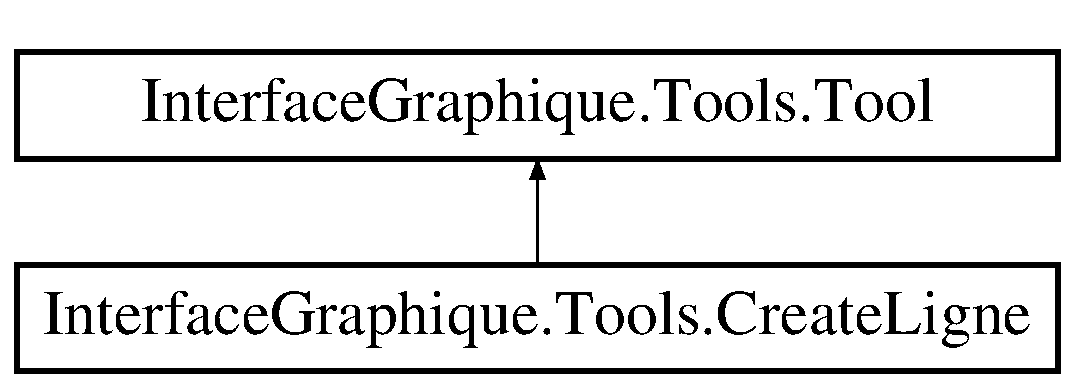
\includegraphics[height=2.000000cm]{class_interface_graphique_1_1_tools_1_1_create_ligne}
\end{center}
\end{figure}
\subsection*{Public Member Functions}
\begin{DoxyCompactItemize}
\item 
\hypertarget{class_interface_graphique_1_1_tools_1_1_create_ligne_a0da55f9f6d189a4e214333cd532c31bc}{}{\bfseries Create\+Ligne} (\hyperlink{class_interface_graphique_1_1_tools_1_1_tool_context}{Tool\+Context} context)\label{class_interface_graphique_1_1_tools_1_1_create_ligne_a0da55f9f6d189a4e214333cd532c31bc}

\item 
\hypertarget{class_interface_graphique_1_1_tools_1_1_create_ligne_a952552e78bc24616026ecd5502dcd0ac}{}override void {\bfseries Left\+Mouse\+Pressed} (Mouse\+Event\+Args e)\label{class_interface_graphique_1_1_tools_1_1_create_ligne_a952552e78bc24616026ecd5502dcd0ac}

\item 
\hypertarget{class_interface_graphique_1_1_tools_1_1_create_ligne_aed5895d2081942fbe80022c99b8de5dc}{}override void {\bfseries Left\+Mouse\+Released} (Mouse\+Event\+Args e)\label{class_interface_graphique_1_1_tools_1_1_create_ligne_aed5895d2081942fbe80022c99b8de5dc}

\item 
\hypertarget{class_interface_graphique_1_1_tools_1_1_create_ligne_a5ea6ec82fe9e433ee36d6ca2fcbf6418}{}override void {\bfseries Left\+Mouse\+Full\+Clicked} (Mouse\+Event\+Args e)\label{class_interface_graphique_1_1_tools_1_1_create_ligne_a5ea6ec82fe9e433ee36d6ca2fcbf6418}

\item 
\hypertarget{class_interface_graphique_1_1_tools_1_1_create_ligne_a5862dbb249d4286c8663e47730a4ec0d}{}override void {\bfseries Dragging} (int delta\+X, int delta\+Y, int delta\+Z)\label{class_interface_graphique_1_1_tools_1_1_create_ligne_a5862dbb249d4286c8663e47730a4ec0d}

\item 
\hypertarget{class_interface_graphique_1_1_tools_1_1_create_ligne_abc111e3dc2d9dfe15050d58631c45564}{}override void {\bfseries Mouse\+Move} (Mouse\+Event\+Args e)\label{class_interface_graphique_1_1_tools_1_1_create_ligne_abc111e3dc2d9dfe15050d58631c45564}

\item 
\hypertarget{class_interface_graphique_1_1_tools_1_1_create_ligne_ad332e361745a2425029bb2c09614d6ef}{}override void {\bfseries esc} ()\label{class_interface_graphique_1_1_tools_1_1_create_ligne_ad332e361745a2425029bb2c09614d6ef}

\end{DoxyCompactItemize}
\subsection*{Public Attributes}
\begin{DoxyCompactItemize}
\item 
\hypertarget{class_interface_graphique_1_1_tools_1_1_create_ligne_abe729b1a7fadece9f5b3f81dff5f994b}{}const string {\bfseries node\+Type} = \char`\"{}ligne\char`\"{}\label{class_interface_graphique_1_1_tools_1_1_create_ligne_abe729b1a7fadece9f5b3f81dff5f994b}

\end{DoxyCompactItemize}


The documentation for this class was generated from the following file\+:\begin{DoxyCompactItemize}
\item 
Sources/\+Interface\+Graphique/\+Tools/Create\+Ligne.\+cs\end{DoxyCompactItemize}

\hypertarget{class_interface_graphique_1_1_tools_1_1_create_mur}{}\section{Interface\+Graphique.\+Tools.\+Create\+Mur Class Reference}
\label{class_interface_graphique_1_1_tools_1_1_create_mur}\index{Interface\+Graphique.\+Tools.\+Create\+Mur@{Interface\+Graphique.\+Tools.\+Create\+Mur}}


Représente l\textquotesingle{}outil de création de murs.  


Inheritance diagram for Interface\+Graphique.\+Tools.\+Create\+Mur\+:\begin{figure}[H]
\begin{center}
\leavevmode
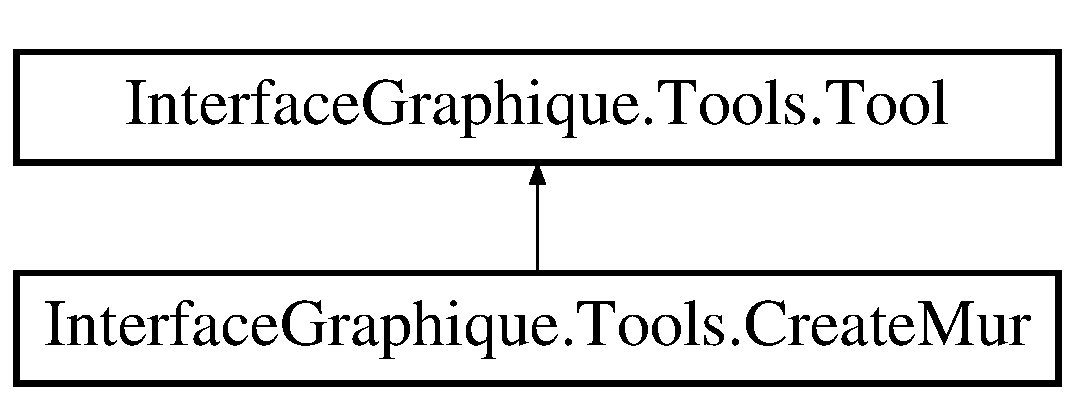
\includegraphics[height=2.000000cm]{class_interface_graphique_1_1_tools_1_1_create_mur}
\end{center}
\end{figure}
\subsection*{Public Member Functions}
\begin{DoxyCompactItemize}
\item 
\hypertarget{class_interface_graphique_1_1_tools_1_1_create_mur_abeb4c3641b9c6677ecc4fb9e7bdbcb6b}{}{\bfseries Create\+Mur} (\hyperlink{class_interface_graphique_1_1_tools_1_1_tool_context}{Tool\+Context} context)\label{class_interface_graphique_1_1_tools_1_1_create_mur_abeb4c3641b9c6677ecc4fb9e7bdbcb6b}

\item 
override void \hyperlink{class_interface_graphique_1_1_tools_1_1_create_mur_a79a1a1f1865df9234e4bd1415ed6b52f}{Left\+Mouse\+Pressed} (Mouse\+Event\+Args e)
\item 
override void \hyperlink{class_interface_graphique_1_1_tools_1_1_create_mur_a663d5c347bf63a1324605eb552c58a19}{Left\+Mouse\+Released} (Mouse\+Event\+Args e)
\item 
override void \hyperlink{class_interface_graphique_1_1_tools_1_1_create_mur_affaacf9919134693a0fc44fe246d4b8c}{Left\+Mouse\+Full\+Clicked} (Mouse\+Event\+Args e)
\item 
override void \hyperlink{class_interface_graphique_1_1_tools_1_1_create_mur_a7ffdf69b104fda7ebdaef67f9ac03582}{Dragging} (int delta\+X, int delta\+Y, int delta\+Z)
\item 
override void \hyperlink{class_interface_graphique_1_1_tools_1_1_create_mur_abe8d1a32d61c3057490450bf9ff2b17c}{Mouse\+Move} (Mouse\+Event\+Args e)
\item 
override void \hyperlink{class_interface_graphique_1_1_tools_1_1_create_mur_a26837d6c8d1fa58b035fb696396fc451}{esc} ()
\end{DoxyCompactItemize}
\subsection*{Public Attributes}
\begin{DoxyCompactItemize}
\item 
\hypertarget{class_interface_graphique_1_1_tools_1_1_create_mur_a6a3194a95fe6d3ec0df213d94936da79}{}const string {\bfseries node\+Type} = \char`\"{}mur\char`\"{}\label{class_interface_graphique_1_1_tools_1_1_create_mur_a6a3194a95fe6d3ec0df213d94936da79}

\end{DoxyCompactItemize}


\subsection{Detailed Description}
Représente l\textquotesingle{}outil de création de murs. 

\begin{DoxyAuthor}{Author}
I\+N\+F2990-\/\+A15-\/01 
\end{DoxyAuthor}
\begin{DoxyDate}{Date}
2015-\/10-\/01 
\end{DoxyDate}


\subsection{Member Function Documentation}
\hypertarget{class_interface_graphique_1_1_tools_1_1_create_mur_a7ffdf69b104fda7ebdaef67f9ac03582}{}\index{Interface\+Graphique\+::\+Tools\+::\+Create\+Mur@{Interface\+Graphique\+::\+Tools\+::\+Create\+Mur}!Dragging@{Dragging}}
\index{Dragging@{Dragging}!Interface\+Graphique\+::\+Tools\+::\+Create\+Mur@{Interface\+Graphique\+::\+Tools\+::\+Create\+Mur}}
\subsubsection[{Dragging(int delta\+X, int delta\+Y, int delta\+Z)}]{\setlength{\rightskip}{0pt plus 5cm}override void Interface\+Graphique.\+Tools.\+Create\+Mur.\+Dragging (
\begin{DoxyParamCaption}
\item[{int}]{delta\+X, }
\item[{int}]{delta\+Y, }
\item[{int}]{delta\+Z}
\end{DoxyParamCaption}
)\hspace{0.3cm}{\ttfamily [inline]}, {\ttfamily [virtual]}}\label{class_interface_graphique_1_1_tools_1_1_create_mur_a7ffdf69b104fda7ebdaef67f9ac03582}
Appelé dès qu\textquotesingle{}on bouge des éléments


\begin{DoxyParams}[1]{Parameters}
\mbox{\tt in}  & {\em delta\+X} & \+: la distance en X \\
\hline
\mbox{\tt in}  & {\em delta\+Y} & \+: la distance en Y \\
\hline
\mbox{\tt in}  & {\em delta\+Z} & \+: la distance en Z\\
\hline
\end{DoxyParams}
\begin{DoxyReturn}{Returns}
Aucun 
\end{DoxyReturn}


Reimplemented from \hyperlink{class_interface_graphique_1_1_tools_1_1_tool_a8b9595e6a3eb55443b8b2cdb38a2c390}{Interface\+Graphique.\+Tools.\+Tool}.

\hypertarget{class_interface_graphique_1_1_tools_1_1_create_mur_a26837d6c8d1fa58b035fb696396fc451}{}\index{Interface\+Graphique\+::\+Tools\+::\+Create\+Mur@{Interface\+Graphique\+::\+Tools\+::\+Create\+Mur}!esc@{esc}}
\index{esc@{esc}!Interface\+Graphique\+::\+Tools\+::\+Create\+Mur@{Interface\+Graphique\+::\+Tools\+::\+Create\+Mur}}
\subsubsection[{esc()}]{\setlength{\rightskip}{0pt plus 5cm}override void Interface\+Graphique.\+Tools.\+Create\+Mur.\+esc (
\begin{DoxyParamCaption}
{}
\end{DoxyParamCaption}
)\hspace{0.3cm}{\ttfamily [inline]}, {\ttfamily [virtual]}}\label{class_interface_graphique_1_1_tools_1_1_create_mur_a26837d6c8d1fa58b035fb696396fc451}
Appelé quand on fait escape

\begin{DoxyReturn}{Returns}
Aucun 
\end{DoxyReturn}


Reimplemented from \hyperlink{class_interface_graphique_1_1_tools_1_1_tool_a734cc3904ce75149652ac356caba93f7}{Interface\+Graphique.\+Tools.\+Tool}.

\hypertarget{class_interface_graphique_1_1_tools_1_1_create_mur_affaacf9919134693a0fc44fe246d4b8c}{}\index{Interface\+Graphique\+::\+Tools\+::\+Create\+Mur@{Interface\+Graphique\+::\+Tools\+::\+Create\+Mur}!Left\+Mouse\+Full\+Clicked@{Left\+Mouse\+Full\+Clicked}}
\index{Left\+Mouse\+Full\+Clicked@{Left\+Mouse\+Full\+Clicked}!Interface\+Graphique\+::\+Tools\+::\+Create\+Mur@{Interface\+Graphique\+::\+Tools\+::\+Create\+Mur}}
\subsubsection[{Left\+Mouse\+Full\+Clicked(\+Mouse\+Event\+Args e)}]{\setlength{\rightskip}{0pt plus 5cm}override void Interface\+Graphique.\+Tools.\+Create\+Mur.\+Left\+Mouse\+Full\+Clicked (
\begin{DoxyParamCaption}
\item[{Mouse\+Event\+Args}]{e}
\end{DoxyParamCaption}
)\hspace{0.3cm}{\ttfamily [inline]}, {\ttfamily [virtual]}}\label{class_interface_graphique_1_1_tools_1_1_create_mur_affaacf9919134693a0fc44fe246d4b8c}
Appelé quand on appuis et relâche sur le bouton gauche de la souris à l\textquotesingle{}intérieur de trois pixels. Représente un click.


\begin{DoxyParams}[1]{Parameters}
\mbox{\tt in}  & {\em e} & \+: les informations sur l\textquotesingle{}événement\\
\hline
\end{DoxyParams}
\begin{DoxyReturn}{Returns}
Aucun 
\end{DoxyReturn}


Reimplemented from \hyperlink{class_interface_graphique_1_1_tools_1_1_tool_a043f210d7840ec8aa5723b193e71ead5}{Interface\+Graphique.\+Tools.\+Tool}.

\hypertarget{class_interface_graphique_1_1_tools_1_1_create_mur_a79a1a1f1865df9234e4bd1415ed6b52f}{}\index{Interface\+Graphique\+::\+Tools\+::\+Create\+Mur@{Interface\+Graphique\+::\+Tools\+::\+Create\+Mur}!Left\+Mouse\+Pressed@{Left\+Mouse\+Pressed}}
\index{Left\+Mouse\+Pressed@{Left\+Mouse\+Pressed}!Interface\+Graphique\+::\+Tools\+::\+Create\+Mur@{Interface\+Graphique\+::\+Tools\+::\+Create\+Mur}}
\subsubsection[{Left\+Mouse\+Pressed(\+Mouse\+Event\+Args e)}]{\setlength{\rightskip}{0pt plus 5cm}override void Interface\+Graphique.\+Tools.\+Create\+Mur.\+Left\+Mouse\+Pressed (
\begin{DoxyParamCaption}
\item[{Mouse\+Event\+Args}]{e}
\end{DoxyParamCaption}
)\hspace{0.3cm}{\ttfamily [inline]}, {\ttfamily [virtual]}}\label{class_interface_graphique_1_1_tools_1_1_create_mur_a79a1a1f1865df9234e4bd1415ed6b52f}
Appelé quand on appuis sur le bouton gauche de la souris


\begin{DoxyParams}[1]{Parameters}
\mbox{\tt in}  & {\em e} & \+: les informations sur l\textquotesingle{}événement\\
\hline
\end{DoxyParams}
\begin{DoxyReturn}{Returns}
Aucun 
\end{DoxyReturn}


Reimplemented from \hyperlink{class_interface_graphique_1_1_tools_1_1_tool_af5c8a4b2773f0d09f45575ade24769ba}{Interface\+Graphique.\+Tools.\+Tool}.

\hypertarget{class_interface_graphique_1_1_tools_1_1_create_mur_a663d5c347bf63a1324605eb552c58a19}{}\index{Interface\+Graphique\+::\+Tools\+::\+Create\+Mur@{Interface\+Graphique\+::\+Tools\+::\+Create\+Mur}!Left\+Mouse\+Released@{Left\+Mouse\+Released}}
\index{Left\+Mouse\+Released@{Left\+Mouse\+Released}!Interface\+Graphique\+::\+Tools\+::\+Create\+Mur@{Interface\+Graphique\+::\+Tools\+::\+Create\+Mur}}
\subsubsection[{Left\+Mouse\+Released(\+Mouse\+Event\+Args e)}]{\setlength{\rightskip}{0pt plus 5cm}override void Interface\+Graphique.\+Tools.\+Create\+Mur.\+Left\+Mouse\+Released (
\begin{DoxyParamCaption}
\item[{Mouse\+Event\+Args}]{e}
\end{DoxyParamCaption}
)\hspace{0.3cm}{\ttfamily [inline]}, {\ttfamily [virtual]}}\label{class_interface_graphique_1_1_tools_1_1_create_mur_a663d5c347bf63a1324605eb552c58a19}
Appelé quand on relâche sur le bouton gauche de la souris


\begin{DoxyParams}[1]{Parameters}
\mbox{\tt in}  & {\em e} & \+: les informations sur l\textquotesingle{}événement\\
\hline
\end{DoxyParams}
\begin{DoxyReturn}{Returns}
Aucun 
\end{DoxyReturn}


Reimplemented from \hyperlink{class_interface_graphique_1_1_tools_1_1_tool_a51c4828f7d24c599b5748b9b3f64d39e}{Interface\+Graphique.\+Tools.\+Tool}.

\hypertarget{class_interface_graphique_1_1_tools_1_1_create_mur_abe8d1a32d61c3057490450bf9ff2b17c}{}\index{Interface\+Graphique\+::\+Tools\+::\+Create\+Mur@{Interface\+Graphique\+::\+Tools\+::\+Create\+Mur}!Mouse\+Move@{Mouse\+Move}}
\index{Mouse\+Move@{Mouse\+Move}!Interface\+Graphique\+::\+Tools\+::\+Create\+Mur@{Interface\+Graphique\+::\+Tools\+::\+Create\+Mur}}
\subsubsection[{Mouse\+Move(\+Mouse\+Event\+Args e)}]{\setlength{\rightskip}{0pt plus 5cm}override void Interface\+Graphique.\+Tools.\+Create\+Mur.\+Mouse\+Move (
\begin{DoxyParamCaption}
\item[{Mouse\+Event\+Args}]{e}
\end{DoxyParamCaption}
)\hspace{0.3cm}{\ttfamily [inline]}, {\ttfamily [virtual]}}\label{class_interface_graphique_1_1_tools_1_1_create_mur_abe8d1a32d61c3057490450bf9ff2b17c}
Appelé quand on bouge la souris


\begin{DoxyParams}[1]{Parameters}
\mbox{\tt in}  & {\em e} & \+: les informations sur l\textquotesingle{}événement\\
\hline
\end{DoxyParams}
\begin{DoxyReturn}{Returns}
Aucun 
\end{DoxyReturn}


Reimplemented from \hyperlink{class_interface_graphique_1_1_tools_1_1_tool_aedd1c93f96ee602475b7cbc3c9c99baa}{Interface\+Graphique.\+Tools.\+Tool}.



The documentation for this class was generated from the following file\+:\begin{DoxyCompactItemize}
\item 
C\+:/\+Users/\+Louis/workspace/inf2990-\/01/\+Sources/\+Interface\+Graphique/\+Tools/Create\+Mur.\+cs\end{DoxyCompactItemize}

\hypertarget{class_interface_graphique_1_1_tools_1_1_create_poteau}{}\section{Interface\+Graphique.\+Tools.\+Create\+Poteau Class Reference}
\label{class_interface_graphique_1_1_tools_1_1_create_poteau}\index{Interface\+Graphique.\+Tools.\+Create\+Poteau@{Interface\+Graphique.\+Tools.\+Create\+Poteau}}
Inheritance diagram for Interface\+Graphique.\+Tools.\+Create\+Poteau\+:\begin{figure}[H]
\begin{center}
\leavevmode
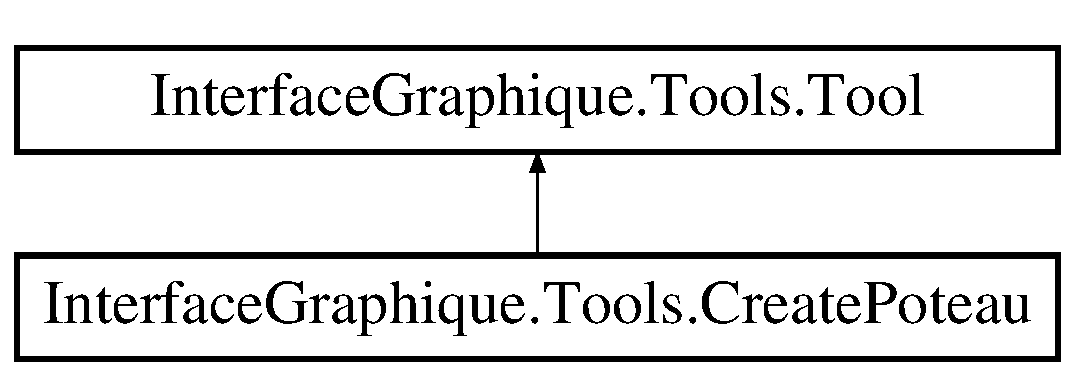
\includegraphics[height=2.000000cm]{class_interface_graphique_1_1_tools_1_1_create_poteau}
\end{center}
\end{figure}
\subsection*{Public Member Functions}
\begin{DoxyCompactItemize}
\item 
\hypertarget{class_interface_graphique_1_1_tools_1_1_create_poteau_a6828c36c0aaa7d27292254045a1b58f2}{}{\bfseries Create\+Poteau} (\hyperlink{class_interface_graphique_1_1_tools_1_1_tool_context}{Tool\+Context} context)\label{class_interface_graphique_1_1_tools_1_1_create_poteau_a6828c36c0aaa7d27292254045a1b58f2}

\item 
\hypertarget{class_interface_graphique_1_1_tools_1_1_create_poteau_a2e2251d85bed79c7b240fc3eb72a29be}{}override void {\bfseries Left\+Mouse\+Pressed} (Mouse\+Event\+Args e)\label{class_interface_graphique_1_1_tools_1_1_create_poteau_a2e2251d85bed79c7b240fc3eb72a29be}

\item 
\hypertarget{class_interface_graphique_1_1_tools_1_1_create_poteau_a1ddd68f567ccb4b8fc5fb06693ec85b1}{}override void {\bfseries Left\+Mouse\+Released} (Mouse\+Event\+Args e)\label{class_interface_graphique_1_1_tools_1_1_create_poteau_a1ddd68f567ccb4b8fc5fb06693ec85b1}

\item 
\hypertarget{class_interface_graphique_1_1_tools_1_1_create_poteau_a659960f2f85f7ff0ff64bd06d2e7cf9c}{}override void {\bfseries Left\+Mouse\+Full\+Clicked} (Mouse\+Event\+Args e)\label{class_interface_graphique_1_1_tools_1_1_create_poteau_a659960f2f85f7ff0ff64bd06d2e7cf9c}

\item 
\hypertarget{class_interface_graphique_1_1_tools_1_1_create_poteau_a30dcd71c461a1afc6fd4dd95c0e2a0ee}{}override void {\bfseries Dragging} (int delta\+X, int delta\+Y, int delta\+Z)\label{class_interface_graphique_1_1_tools_1_1_create_poteau_a30dcd71c461a1afc6fd4dd95c0e2a0ee}

\item 
\hypertarget{class_interface_graphique_1_1_tools_1_1_create_poteau_a11cb39fe881af64c1be87c44cc1c8306}{}override void {\bfseries Mouse\+Move} (Mouse\+Event\+Args e)\label{class_interface_graphique_1_1_tools_1_1_create_poteau_a11cb39fe881af64c1be87c44cc1c8306}

\item 
\hypertarget{class_interface_graphique_1_1_tools_1_1_create_poteau_a523af264dfe1487c08d1d73b309a1095}{}override void {\bfseries esc} ()\label{class_interface_graphique_1_1_tools_1_1_create_poteau_a523af264dfe1487c08d1d73b309a1095}

\end{DoxyCompactItemize}
\subsection*{Public Attributes}
\begin{DoxyCompactItemize}
\item 
\hypertarget{class_interface_graphique_1_1_tools_1_1_create_poteau_afbc3cc3c600255e7d9d12cf06b082a04}{}const string {\bfseries node\+Type} = \char`\"{}cylindre\char`\"{}\label{class_interface_graphique_1_1_tools_1_1_create_poteau_afbc3cc3c600255e7d9d12cf06b082a04}

\end{DoxyCompactItemize}


The documentation for this class was generated from the following file\+:\begin{DoxyCompactItemize}
\item 
Sources/\+Interface\+Graphique/\+Tools/Create\+Poteau.\+cs\end{DoxyCompactItemize}

\hypertarget{structutilitaire_1_1_cylindre_englobant}{}\section{utilitaire\+:\+:Cylindre\+Englobant Struct Reference}
\label{structutilitaire_1_1_cylindre_englobant}\index{utilitaire\+::\+Cylindre\+Englobant@{utilitaire\+::\+Cylindre\+Englobant}}


Structure contenant les données pour un cylindre englobant.  




{\ttfamily \#include $<$Utilitaire.\+h$>$}

\subsection*{Public Attributes}
\begin{DoxyCompactItemize}
\item 
\hypertarget{structutilitaire_1_1_cylindre_englobant_abbec6b7a8f2790f286317ffcdeab476c}{}double {\bfseries rayon}\label{structutilitaire_1_1_cylindre_englobant_abbec6b7a8f2790f286317ffcdeab476c}

\item 
\hypertarget{structutilitaire_1_1_cylindre_englobant_ac99c3cebbc6829ad9f54e392f4525e7e}{}double {\bfseries bas}\label{structutilitaire_1_1_cylindre_englobant_ac99c3cebbc6829ad9f54e392f4525e7e}

\item 
\hypertarget{structutilitaire_1_1_cylindre_englobant_a9f86204ad37c5b04fb329b710304c459}{}double {\bfseries haut}\label{structutilitaire_1_1_cylindre_englobant_a9f86204ad37c5b04fb329b710304c459}

\end{DoxyCompactItemize}


\subsection{Detailed Description}
Structure contenant les données pour un cylindre englobant. 

The documentation for this struct was generated from the following file\+:\begin{DoxyCompactItemize}
\item 
C\+:/\+Users/\+Louis/workspace/inf2990-\/01/\+Commun/\+Utilitaire/\hyperlink{_utilitaire_8h}{Utilitaire.\+h}\end{DoxyCompactItemize}

\hypertarget{class_interface_graphique_1_1_debug}{}\section{Interface\+Graphique.\+Debug Class Reference}
\label{class_interface_graphique_1_1_debug}\index{Interface\+Graphique.\+Debug@{Interface\+Graphique.\+Debug}}
\subsection*{Static Public Member Functions}
\begin{DoxyCompactItemize}
\item 
\hypertarget{class_interface_graphique_1_1_debug_a540c6c5d53e75f5710492b0254eaf0a3}{}static void {\bfseries Write} (String msg, params object\mbox{[}$\,$\mbox{]} data)\label{class_interface_graphique_1_1_debug_a540c6c5d53e75f5710492b0254eaf0a3}

\item 
\hypertarget{class_interface_graphique_1_1_debug_a86721cc22d894c08f05abfb82e07f494}{}static bool {\bfseries Is\+Debug\+Enabled} ()\label{class_interface_graphique_1_1_debug_a86721cc22d894c08f05abfb82e07f494}

\end{DoxyCompactItemize}


The documentation for this class was generated from the following file\+:\begin{DoxyCompactItemize}
\item 
C\+:/\+Users/\+Louis/workspace/inf2990-\/01/\+Sources/\+Interface\+Graphique/Debug.\+cs\end{DoxyCompactItemize}

\hypertarget{class_debug}{\section{Référence de la classe Debug}
\label{class_debug}\index{Debug@{Debug}}
}


Classe gérant l'affichage d'informations à la console et les informations de déboguage à afficher ou non.  




{\ttfamily \#include $<$Debug.\-h$>$}

\subsection*{Types publics}
\begin{DoxyCompactItemize}
\item 
enum \hyperlink{class_debug_afd6ed3c50c08d0a7830cd5253b4ab8b6}{Declencheur} \{ \\*
{\bfseries C\-O\-N\-S\-O\-L\-E}, 
{\bfseries T\-E\-S\-T}, 
{\bfseries C\-A\-P\-T\-E\-U\-R\-\_\-\-G\-A\-U\-C\-H\-E\-\_\-\-S\-A\-F\-E}, 
{\bfseries C\-A\-P\-T\-E\-U\-R\-\_\-\-G\-A\-U\-C\-H\-E\-\_\-\-D\-A\-N\-G\-E\-R}, 
\\*
{\bfseries C\-A\-P\-T\-E\-U\-R\-\_\-\-C\-E\-N\-T\-R\-E\-\_\-\-S\-A\-F\-E}, 
{\bfseries C\-A\-P\-T\-E\-U\-R\-\_\-\-C\-E\-N\-T\-R\-E\-\_\-\-D\-A\-N\-G\-E\-R}, 
{\bfseries C\-A\-P\-T\-E\-U\-R\-\_\-\-D\-R\-O\-I\-T\-\_\-\-S\-A\-F\-E}, 
{\bfseries C\-A\-P\-T\-E\-U\-R\-\_\-\-D\-R\-O\-I\-T\-\_\-\-D\-A\-N\-G\-E\-R}, 
\\*
{\bfseries B\-A\-L\-A\-Y\-A\-G\-E}, 
{\bfseries L\-U\-M\-\_\-\-A\-M\-B\-I\-A\-N\-T\-E}, 
{\bfseries L\-U\-M\-\_\-\-D\-I\-R\-E\-C\-T\-I\-O\-N\-N\-E\-L\-L\-E}, 
{\bfseries L\-U\-M\-\_\-\-S\-P\-O\-T}, 
\\*
{\bfseries C\-O\-L\-L\-I\-S\-I\-O\-N}
 \}
\begin{DoxyCompactList}\small\item\em Déclencheurs possibles pour les messages et activation de debug. \end{DoxyCompactList}\end{DoxyCompactItemize}
\subsection*{Fonctions membres publiques}
\begin{DoxyCompactItemize}
\item 
void \hyperlink{group__inf2990_ga0d51f3d912211a1e4ff8232c04db8174}{print\-Message} (\hyperlink{class_debug_afd6ed3c50c08d0a7830cd5253b4ab8b6}{Declencheur} declencheur, std\-::string message)
\begin{DoxyCompactList}\small\item\em Affiche un message à la console. \end{DoxyCompactList}\item 
void \hyperlink{group__inf2990_ga45d10d28492f6a29f44335e0f479e1f6}{print\-Error} (\hyperlink{class_debug_afd6ed3c50c08d0a7830cd5253b4ab8b6}{Declencheur} declencheur, std\-::string message)
\begin{DoxyCompactList}\small\item\em Affiche une erreur à la console. \end{DoxyCompactList}\item 
std\-::string \hyperlink{group__inf2990_gae0f25a128c40b3019a2351d3fb1e938b}{get\-Current\-Time\-\_\-precise} () const 
\begin{DoxyCompactList}\small\item\em Retourne le temps actuel sous le format H\-H\-:\-M\-M\-:\-S\-S\-:mmm. \end{DoxyCompactList}\item 
std\-::string \hyperlink{group__inf2990_ga6de3f26eda6414f573d0c5f64f711dc3}{get\-Current\-Time\-\_\-generic} () const 
\begin{DoxyCompactList}\small\item\em Retourne le temps actuel sous le format A\-A\-A\-A-\/\-M\-M-\/\-J\-J-\/hhmm. \end{DoxyCompactList}\item 
void \hyperlink{group__inf2990_gabf9d25ff2565e30a1f481e39e4e2192f}{enable\-Log} ()
\begin{DoxyCompactList}\small\item\em Active la sortie journal. \end{DoxyCompactList}\item 
void \hyperlink{group__inf2990_ga05742456a67e8e3104a3a6d0134c58ed}{disable\-Log} ()
\begin{DoxyCompactList}\small\item\em Désactive la sortie journal. \end{DoxyCompactList}\item 
void \hyperlink{group__inf2990_gafa37fad6a0a050a913eb0e482f1b0282}{set\-Log} (bool enabled)
\begin{DoxyCompactList}\small\item\em Assigne la sortie journal. \end{DoxyCompactList}\item 
bool \hyperlink{group__inf2990_gae22799c006444ad7f48e7de490b41ef0}{is\-Log\-Enabled} () const 
\begin{DoxyCompactList}\small\item\em Retourne l'état d'utilsation du journal. \end{DoxyCompactList}\item 
void \hyperlink{group__inf2990_ga55375c6c14be967ed7f25eed578a6265}{enable\-Type} (\hyperlink{class_debug_afd6ed3c50c08d0a7830cd5253b4ab8b6}{Declencheur} declencheur)
\begin{DoxyCompactList}\small\item\em Active les informations de déboguage d'un déclencheur. \end{DoxyCompactList}\item 
void \hyperlink{group__inf2990_gaefa863abf2c2b3c6c741b88b3f78e8b3}{disable\-Type} (\hyperlink{class_debug_afd6ed3c50c08d0a7830cd5253b4ab8b6}{Declencheur} declencheur)
\begin{DoxyCompactList}\small\item\em Désactive les informations de déboguage d'un déclencheur. \end{DoxyCompactList}\item 
void \hyperlink{group__inf2990_gaf6b5623dc8f2fdc90abb3648499f3415}{set\-Type} (\hyperlink{class_debug_afd6ed3c50c08d0a7830cd5253b4ab8b6}{Declencheur} declencheur, bool enabled)
\begin{DoxyCompactList}\small\item\em Assigne l'activation des informations de déboguage d'un déclencheur. \end{DoxyCompactList}\item 
void \hyperlink{group__inf2990_gaba1a061318eb0f1819f0c02754b3cb62}{set\-Triggers} (\hyperlink{struct_debug_settings}{Debug\-Settings} settings)
\begin{DoxyCompactList}\small\item\em Assigne l'activation des informations de déboguage des déclencheurs. \end{DoxyCompactList}\item 
bool \hyperlink{group__inf2990_ga63c334cf7a3be794bb8b349c4938613d}{is\-Enabled} (\hyperlink{class_debug_afd6ed3c50c08d0a7830cd5253b4ab8b6}{Declencheur} declencheur)
\begin{DoxyCompactList}\small\item\em Retourne l'état d'activation d'un déclencheur. \end{DoxyCompactList}\item 
bool \hyperlink{group__inf2990_ga15e281e19fa3282487c656ad14d55ee4}{visuals\-Enabled} () const 
\begin{DoxyCompactList}\small\item\em Retourne l'état d'activation des informations visuelles. \end{DoxyCompactList}\end{DoxyCompactItemize}
\subsection*{Fonctions membres publiques statiques}
\begin{DoxyCompactItemize}
\item 
static \hyperlink{class_debug}{Debug} $\ast$ \hyperlink{group__inf2990_ga823bf701dd9f4c706143dca1e8666941}{get\-Instance} ()
\begin{DoxyCompactList}\small\item\em Obtient l'instance unique de la classe. \end{DoxyCompactList}\item 
static void \hyperlink{group__inf2990_gacaafb83305279aafab24735adc903931}{reset\-Instance} ()
\begin{DoxyCompactList}\small\item\em Libère l'instance unique de la classe. \end{DoxyCompactList}\end{DoxyCompactItemize}


\subsection{Description détaillée}
Classe gérant l'affichage d'informations à la console et les informations de déboguage à afficher ou non. 

\begin{DoxyAuthor}{Auteur}
I\-N\-F2990-\/\-A15-\/01 
\end{DoxyAuthor}
\begin{DoxyDate}{Date}
2015-\/09-\/09 
\end{DoxyDate}


La documentation de cette classe a été générée à partir des fichiers suivants \-:\begin{DoxyCompactItemize}
\item 
C\-:/\-Users/saron/\-Documents/inf2990-\/01/\-Sources/\-D\-L\-L/\-Application/\hyperlink{_debug_8h}{Debug.\-h}\item 
C\-:/\-Users/saron/\-Documents/inf2990-\/01/\-Sources/\-D\-L\-L/\-Application/\hyperlink{_debug_8cpp}{Debug.\-cpp}\end{DoxyCompactItemize}

\hypertarget{class_interface_graphique_1_1_debug_select}{\section{Référence de la classe Interface\-Graphique.\-Debug\-Select}
\label{class_interface_graphique_1_1_debug_select}\index{Interface\-Graphique.\-Debug\-Select@{Interface\-Graphique.\-Debug\-Select}}
}


Interaction logic for User\-Control2.\-xaml  


Graphe d'héritage de Interface\-Graphique.\-Debug\-Select\-:\begin{figure}[H]
\begin{center}
\leavevmode
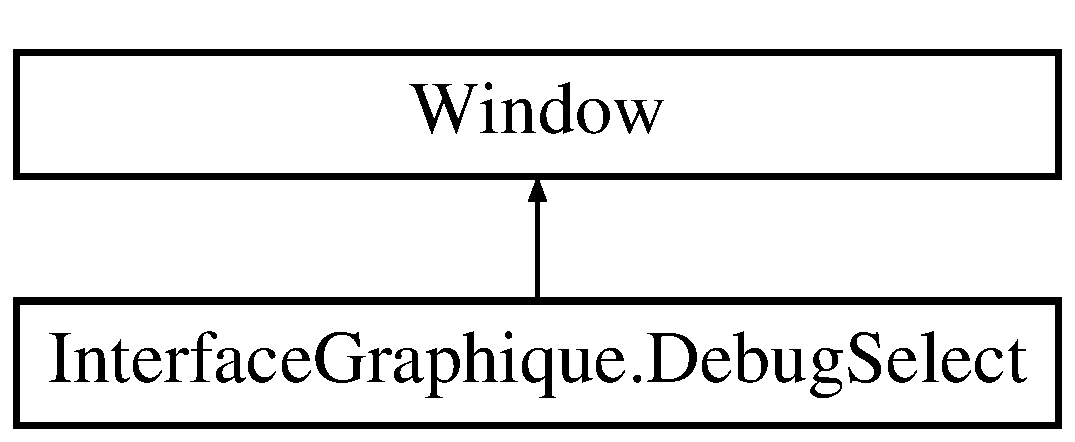
\includegraphics[height=2.000000cm]{class_interface_graphique_1_1_debug_select}
\end{center}
\end{figure}


\subsection{Description détaillée}
Interaction logic for User\-Control2.\-xaml 

Tiré de \href{http://wpftutorial.net/Home.html}{\tt http\-://wpftutorial.\-net/\-Home.\-html} 

La documentation de cette classe a été générée à partir du fichier suivant \-:\begin{DoxyCompactItemize}
\item 
C\-:/\-Users/saron/\-Documents/inf2990-\/01/\-Sources/\-Interface\-Graphique/Debug\-Select.\-xaml.\-cs\end{DoxyCompactItemize}

\hypertarget{struct_debug_settings}{\section{Référence de la structure Debug\-Settings}
\label{struct_debug_settings}\index{Debug\-Settings@{Debug\-Settings}}
}
\subsection*{Attributs publics}
\begin{DoxyCompactItemize}
\item 
\hypertarget{struct_debug_settings_abd553e888464f3fd02ed933499516a1a}{int {\bfseries C\-O\-N\-S\-O\-L\-E}}\label{struct_debug_settings_abd553e888464f3fd02ed933499516a1a}

\item 
\hypertarget{struct_debug_settings_acf8aa9d1b832e4b2561ec3327af30638}{int {\bfseries T\-E\-S\-T}}\label{struct_debug_settings_acf8aa9d1b832e4b2561ec3327af30638}

\item 
\hypertarget{struct_debug_settings_acca84580e91ec56cfb2a38754c925102}{int {\bfseries C\-A\-P\-T\-E\-U\-R\-\_\-\-G\-A\-U\-C\-H\-E\-\_\-\-S\-A\-F\-E}}\label{struct_debug_settings_acca84580e91ec56cfb2a38754c925102}

\item 
\hypertarget{struct_debug_settings_ae72bb96e51715636053afe813e5f775f}{int {\bfseries C\-A\-P\-T\-E\-U\-R\-\_\-\-G\-A\-U\-C\-H\-E\-\_\-\-D\-A\-N\-G\-E\-R}}\label{struct_debug_settings_ae72bb96e51715636053afe813e5f775f}

\item 
\hypertarget{struct_debug_settings_ab09721cb0c21668eae5e54c5aa559ce4}{int {\bfseries C\-A\-P\-T\-E\-U\-R\-\_\-\-C\-E\-N\-T\-R\-E\-\_\-\-S\-A\-F\-E}}\label{struct_debug_settings_ab09721cb0c21668eae5e54c5aa559ce4}

\item 
\hypertarget{struct_debug_settings_ac9f0fcaa06d4bcc01c754431e073ce2b}{int {\bfseries C\-A\-P\-T\-E\-U\-R\-\_\-\-C\-E\-N\-T\-R\-E\-\_\-\-D\-A\-N\-G\-E\-R}}\label{struct_debug_settings_ac9f0fcaa06d4bcc01c754431e073ce2b}

\item 
\hypertarget{struct_debug_settings_a691e13b0b84d60b2d1f309f7c2ccf3b3}{int {\bfseries C\-A\-P\-T\-E\-U\-R\-\_\-\-D\-R\-O\-I\-T\-\_\-\-S\-A\-F\-E}}\label{struct_debug_settings_a691e13b0b84d60b2d1f309f7c2ccf3b3}

\item 
\hypertarget{struct_debug_settings_a50361b94f264c2c0bacba3a51bc78e02}{int {\bfseries C\-A\-P\-T\-E\-U\-R\-\_\-\-D\-R\-O\-I\-T\-\_\-\-D\-A\-N\-G\-E\-R}}\label{struct_debug_settings_a50361b94f264c2c0bacba3a51bc78e02}

\item 
\hypertarget{struct_debug_settings_a57e0ebb7811bf1d6877585fb87fb6719}{int {\bfseries B\-A\-L\-A\-Y\-A\-G\-E}}\label{struct_debug_settings_a57e0ebb7811bf1d6877585fb87fb6719}

\item 
\hypertarget{struct_debug_settings_a8bf6bc8f82dbd71e95bca1c52d719c65}{int {\bfseries L\-U\-M\-\_\-\-A\-M\-B\-I\-A\-N\-T\-E}}\label{struct_debug_settings_a8bf6bc8f82dbd71e95bca1c52d719c65}

\item 
\hypertarget{struct_debug_settings_a0b535811647b96b079ca70147c04f91c}{int {\bfseries L\-U\-M\-\_\-\-D\-I\-R\-E\-C\-T\-I\-O\-N\-N\-E\-L\-L\-E}}\label{struct_debug_settings_a0b535811647b96b079ca70147c04f91c}

\item 
\hypertarget{struct_debug_settings_a78e0a9e672944020d9e5afa05c807943}{int {\bfseries L\-U\-M\-\_\-\-S\-P\-O\-T}}\label{struct_debug_settings_a78e0a9e672944020d9e5afa05c807943}

\item 
\hypertarget{struct_debug_settings_af81b8bd5c23bc5db501815a459ed133f}{int {\bfseries C\-O\-L\-L\-I\-S\-I\-O\-N}}\label{struct_debug_settings_af81b8bd5c23bc5db501815a459ed133f}

\item 
\hypertarget{struct_debug_settings_aaa5bc236f86ae8d4cde2e688664d320f}{int {\bfseries V\-I\-S\-U\-A\-L\-S}}\label{struct_debug_settings_aaa5bc236f86ae8d4cde2e688664d320f}

\item 
\hypertarget{struct_debug_settings_a525d4e651a6c101c31739183185b1834}{int {\bfseries L\-O\-G}}\label{struct_debug_settings_a525d4e651a6c101c31739183185b1834}

\end{DoxyCompactItemize}


La documentation de cette structure a été générée à partir du fichier suivant \-:\begin{DoxyCompactItemize}
\item 
C\-:/\-Users/saron/\-Documents/inf2990-\/01/\-Sources/\-D\-L\-L/\-Interface/Debug\-Settings.\-h\end{DoxyCompactItemize}

\hypertarget{struct_interface_graphique_1_1_debug_settings}{\section{Référence de la structure Interface\-Graphique.\-Debug\-Settings}
\label{struct_interface_graphique_1_1_debug_settings}\index{Interface\-Graphique.\-Debug\-Settings@{Interface\-Graphique.\-Debug\-Settings}}
}
\subsection*{Attributs publics}
\begin{DoxyCompactItemize}
\item 
\hypertarget{struct_interface_graphique_1_1_debug_settings_a67a67736b4e45c7ce270de3317469ada}{int {\bfseries C\-O\-N\-S\-O\-L\-E}}\label{struct_interface_graphique_1_1_debug_settings_a67a67736b4e45c7ce270de3317469ada}

\item 
\hypertarget{struct_interface_graphique_1_1_debug_settings_a6c60bc0916961e2b95ead9e0e70a01b9}{int {\bfseries T\-E\-S\-T}}\label{struct_interface_graphique_1_1_debug_settings_a6c60bc0916961e2b95ead9e0e70a01b9}

\item 
\hypertarget{struct_interface_graphique_1_1_debug_settings_aef2863767ba6b929c2e6f53e166b1cec}{int {\bfseries C\-A\-P\-T\-E\-U\-R\-\_\-\-G\-A\-U\-C\-H\-E\-\_\-\-S\-A\-F\-E}}\label{struct_interface_graphique_1_1_debug_settings_aef2863767ba6b929c2e6f53e166b1cec}

\item 
\hypertarget{struct_interface_graphique_1_1_debug_settings_ac2c8f2082e21c76a4331a0a4db087ef7}{int {\bfseries C\-A\-P\-T\-E\-U\-R\-\_\-\-G\-A\-U\-C\-H\-E\-\_\-\-D\-A\-N\-G\-E\-R}}\label{struct_interface_graphique_1_1_debug_settings_ac2c8f2082e21c76a4331a0a4db087ef7}

\item 
\hypertarget{struct_interface_graphique_1_1_debug_settings_aa3bad45d846437894adeeee56b265d09}{int {\bfseries C\-A\-P\-T\-E\-U\-R\-\_\-\-C\-E\-N\-T\-R\-E\-\_\-\-S\-A\-F\-E}}\label{struct_interface_graphique_1_1_debug_settings_aa3bad45d846437894adeeee56b265d09}

\item 
\hypertarget{struct_interface_graphique_1_1_debug_settings_a53903de990d0f98798d6c8e122935c55}{int {\bfseries C\-A\-P\-T\-E\-U\-R\-\_\-\-C\-E\-N\-T\-R\-E\-\_\-\-D\-A\-N\-G\-E\-R}}\label{struct_interface_graphique_1_1_debug_settings_a53903de990d0f98798d6c8e122935c55}

\item 
\hypertarget{struct_interface_graphique_1_1_debug_settings_a0323937a17c31dca0e8470ada9171889}{int {\bfseries C\-A\-P\-T\-E\-U\-R\-\_\-\-D\-R\-O\-I\-T\-\_\-\-S\-A\-F\-E}}\label{struct_interface_graphique_1_1_debug_settings_a0323937a17c31dca0e8470ada9171889}

\item 
\hypertarget{struct_interface_graphique_1_1_debug_settings_a1ae2dbc2bf32f43ba5d6fc38af2e1983}{int {\bfseries C\-A\-P\-T\-E\-U\-R\-\_\-\-D\-R\-O\-I\-T\-\_\-\-D\-A\-N\-G\-E\-R}}\label{struct_interface_graphique_1_1_debug_settings_a1ae2dbc2bf32f43ba5d6fc38af2e1983}

\item 
\hypertarget{struct_interface_graphique_1_1_debug_settings_afd90bbf00846ddf8db271ea800569ac6}{int {\bfseries B\-A\-L\-A\-Y\-A\-G\-E}}\label{struct_interface_graphique_1_1_debug_settings_afd90bbf00846ddf8db271ea800569ac6}

\item 
\hypertarget{struct_interface_graphique_1_1_debug_settings_a13cd4cccdf207a03bd0de2e9d66a0464}{int {\bfseries L\-U\-M\-\_\-\-A\-M\-B\-I\-A\-N\-T\-E}}\label{struct_interface_graphique_1_1_debug_settings_a13cd4cccdf207a03bd0de2e9d66a0464}

\item 
\hypertarget{struct_interface_graphique_1_1_debug_settings_abcdf6c594ee2be7c6334058923fd6782}{int {\bfseries L\-U\-M\-\_\-\-D\-I\-R\-E\-C\-T\-I\-O\-N\-N\-E\-L\-L\-E}}\label{struct_interface_graphique_1_1_debug_settings_abcdf6c594ee2be7c6334058923fd6782}

\item 
\hypertarget{struct_interface_graphique_1_1_debug_settings_a829f4f49fcad36b63a8efa04013b21e2}{int {\bfseries L\-U\-M\-\_\-\-S\-P\-O\-T}}\label{struct_interface_graphique_1_1_debug_settings_a829f4f49fcad36b63a8efa04013b21e2}

\item 
\hypertarget{struct_interface_graphique_1_1_debug_settings_a33ca4cb1f95d52b3036b5653a19e10a7}{int {\bfseries C\-O\-L\-L\-I\-S\-I\-O\-N}}\label{struct_interface_graphique_1_1_debug_settings_a33ca4cb1f95d52b3036b5653a19e10a7}

\item 
\hypertarget{struct_interface_graphique_1_1_debug_settings_a54278ff77bdbcb736e7156e76cd43a75}{int {\bfseries V\-I\-S\-U\-A\-L\-S}}\label{struct_interface_graphique_1_1_debug_settings_a54278ff77bdbcb736e7156e76cd43a75}

\item 
\hypertarget{struct_interface_graphique_1_1_debug_settings_a590cd73799d00b0bb2bc7cd9f570f36e}{int {\bfseries L\-O\-G}}\label{struct_interface_graphique_1_1_debug_settings_a590cd73799d00b0bb2bc7cd9f570f36e}

\end{DoxyCompactItemize}


La documentation de cette structure a été générée à partir du fichier suivant \-:\begin{DoxyCompactItemize}
\item 
C\-:/\-Users/saron/\-Documents/inf2990-\/01/\-Sources/\-Interface\-Graphique/Settings.\-cs\end{DoxyCompactItemize}

\hypertarget{class_default_behavior}{\section{Référence de la classe Default\-Behavior}
\label{class_default_behavior}\index{Default\-Behavior@{Default\-Behavior}}
}


Classe Etat du comportement par defaut.  




{\ttfamily \#include $<$Default\-Behavior.\-h$>$}

Graphe d'héritage de Default\-Behavior\-:\begin{figure}[H]
\begin{center}
\leavevmode
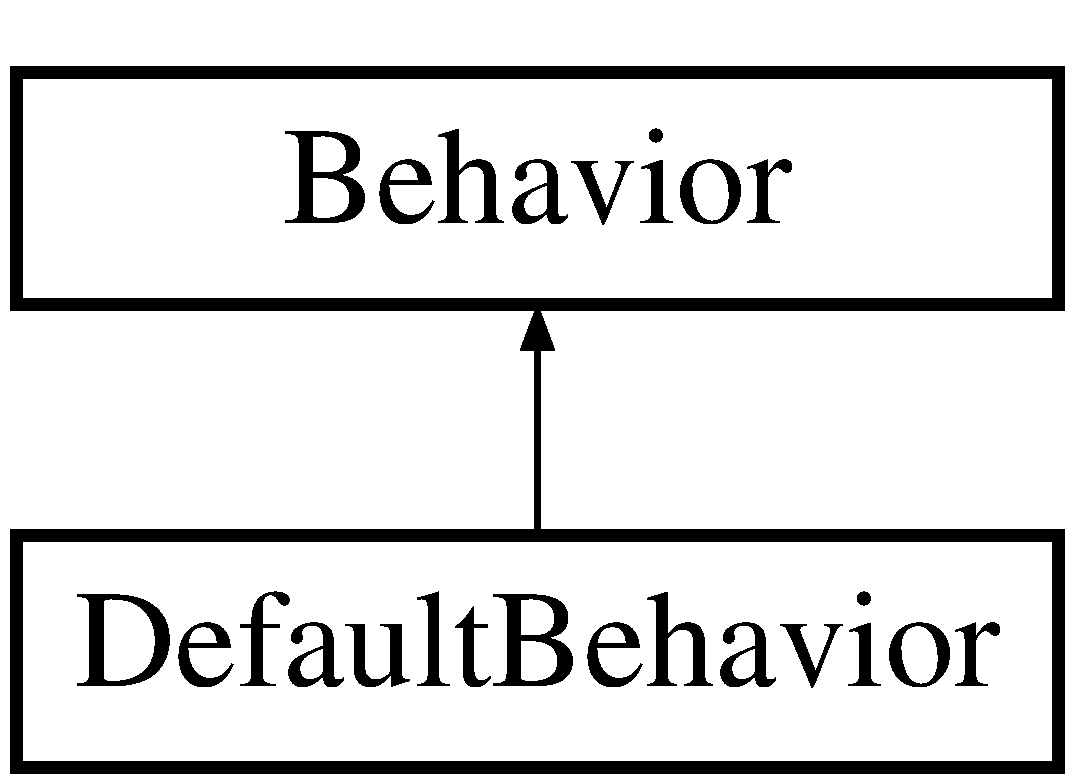
\includegraphics[height=2.000000cm]{class_default_behavior}
\end{center}
\end{figure}
\subsection*{Fonctions membres publiques}
{\bf }\par
\begin{DoxyCompactItemize}
\item 
\hyperlink{class_default_behavior_a8963f21041fd7c653042b40ad81452b1}{Default\-Behavior} (\hyperlink{class_behavior_context}{Behavior\-Context} $\ast$context)
\begin{DoxyCompactList}\small\item\em Constructeur. \end{DoxyCompactList}\item 
void \hyperlink{class_default_behavior_a081682eb85139bf45080ff0787ccd8ca}{do\-Action} () override
\begin{DoxyCompactList}\small\item\em Effectue une etape de son comportement. \end{DoxyCompactList}\end{DoxyCompactItemize}

\subsection*{Membres hérités additionnels}


\subsection{Description détaillée}
Classe Etat du comportement par defaut. 

\subsection{Documentation des constructeurs et destructeur}
\hypertarget{class_default_behavior_a8963f21041fd7c653042b40ad81452b1}{\index{Default\-Behavior@{Default\-Behavior}!Default\-Behavior@{Default\-Behavior}}
\index{Default\-Behavior@{Default\-Behavior}!DefaultBehavior@{Default\-Behavior}}
\subsubsection[{Default\-Behavior}]{\setlength{\rightskip}{0pt plus 5cm}Default\-Behavior\-::\-Default\-Behavior (
\begin{DoxyParamCaption}
\item[{{\bf Behavior\-Context} $\ast$}]{context}
\end{DoxyParamCaption}
)}}\label{class_default_behavior_a8963f21041fd7c653042b40ad81452b1}


Constructeur. 

Constructeur


\begin{DoxyParams}[1]{Paramètres}
\mbox{\tt in}  & {\em context} & \-: La classe pouvant accéder au robot.\\
\hline
\end{DoxyParams}
\begin{DoxyReturn}{Renvoie}
Aucune. 
\end{DoxyReturn}


\subsection{Documentation des fonctions membres}
\hypertarget{class_default_behavior_a081682eb85139bf45080ff0787ccd8ca}{\index{Default\-Behavior@{Default\-Behavior}!do\-Action@{do\-Action}}
\index{do\-Action@{do\-Action}!DefaultBehavior@{Default\-Behavior}}
\subsubsection[{do\-Action}]{\setlength{\rightskip}{0pt plus 5cm}void Default\-Behavior\-::do\-Action (
\begin{DoxyParamCaption}
{}
\end{DoxyParamCaption}
)\hspace{0.3cm}{\ttfamily [override]}, {\ttfamily [virtual]}}}\label{class_default_behavior_a081682eb85139bf45080ff0787ccd8ca}


Effectue une etape de son comportement. 

Cette fonction effectue le comportement de l'état actuel.


\begin{DoxyParams}[1]{Paramètres}
\mbox{\tt in}  & {\em Aucun.} & \\
\hline
\end{DoxyParams}
\begin{DoxyReturn}{Renvoie}
Aucune. 
\end{DoxyReturn}


Réimplémentée à partir de \hyperlink{group__inf2990_gac22f205bc85075ff707ad1f695c18439}{Behavior}.



La documentation de cette classe a été générée à partir des fichiers suivants \-:\begin{DoxyCompactItemize}
\item 
C\-:/\-Users/saron/\-Documents/inf2990-\/01/\-Sources/\-D\-L\-L/\-Behavior/\hyperlink{_default_behavior_8h}{Default\-Behavior.\-h}\item 
C\-:/\-Users/saron/\-Documents/inf2990-\/01/\-Sources/\-D\-L\-L/\-Behavior/\hyperlink{_default_behavior_8cpp}{Default\-Behavior.\-cpp}\end{DoxyCompactItemize}

\hypertarget{class_delete_tool}{}\section{Delete\+Tool Class Reference}
\label{class_delete_tool}\index{Delete\+Tool@{Delete\+Tool}}


Classe concrète héritant de \hyperlink{class_tool}{Tool}, qui effectue l\textquotesingle{}opération de suppression sur un noeud de l\textquotesingle{}arbre de rendu.  




{\ttfamily \#include $<$Delete\+Tool.\+h$>$}

Inheritance diagram for Delete\+Tool\+:\begin{figure}[H]
\begin{center}
\leavevmode
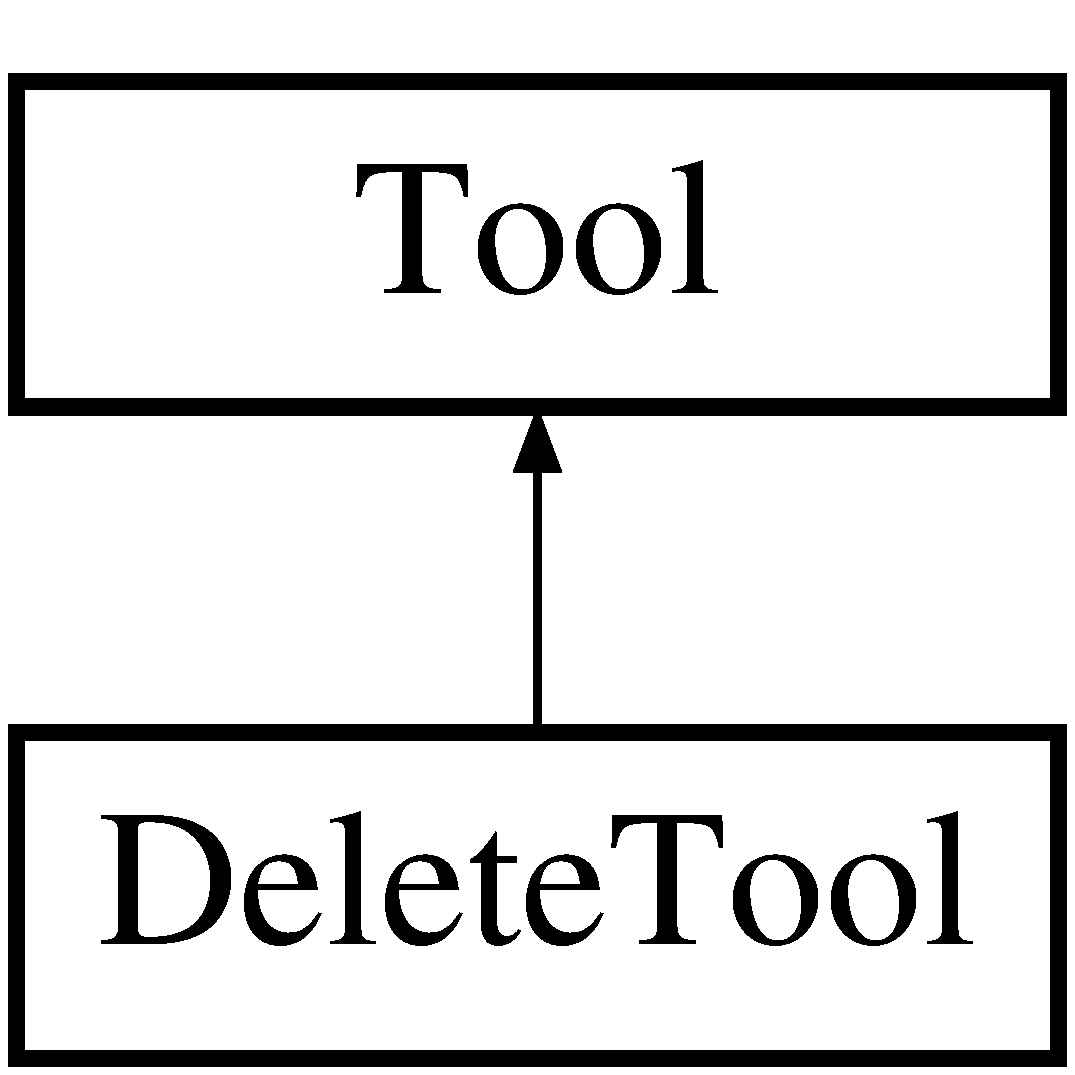
\includegraphics[height=2.000000cm]{class_delete_tool}
\end{center}
\end{figure}
\subsection*{Public Member Functions}
\begin{DoxyCompactItemize}
\item 
\hyperlink{group__inf2990_ga4a54f710ae3ca5e4eb8e16610d07c3bc}{$\sim$\+Delete\+Tool} ()
\item 
void \hyperlink{group__inf2990_gaf91f134881ce52596486855f405e8f96}{visit} (\hyperlink{class_noeud_cylindre}{Noeud\+Cylindre} $\ast$node) override
\item 
void \hyperlink{group__inf2990_ga9efc126da05a809724a3a2597ac4cb57}{visit} (\hyperlink{class_noeud_depart}{Noeud\+Depart} $\ast$node) override
\item 
void \hyperlink{group__inf2990_ga1908b4ee57bb2dfbf4022412b48470d8}{visit} (\hyperlink{class_noeud_segment_concret}{Noeud\+Segment\+Concret} $\ast$node) override
\item 
void \hyperlink{group__inf2990_ga816147276bc393b0552e031441541726}{visit} (\hyperlink{class_noeud_mur}{Noeud\+Mur} $\ast$node) override
\item 
void \hyperlink{group__inf2990_gab16541bc54ef7e060c56d59d64798805}{default\+Delete} (\hyperlink{class_noeud_abstrait}{Noeud\+Abstrait} $\ast$node)
\begin{DoxyCompactList}\small\item\em Algorithme par défaut. \end{DoxyCompactList}\end{DoxyCompactItemize}


\subsection{Detailed Description}
Classe concrète héritant de \hyperlink{class_tool}{Tool}, qui effectue l\textquotesingle{}opération de suppression sur un noeud de l\textquotesingle{}arbre de rendu. 

\begin{DoxyAuthor}{Author}
I\+N\+F2990-\/\+A15-\/01 
\end{DoxyAuthor}
\begin{DoxyDate}{Date}
2015-\/09-\/14 
\end{DoxyDate}


The documentation for this class was generated from the following files\+:\begin{DoxyCompactItemize}
\item 
Sources/\+D\+L\+L/\+Application/\+Visitor/\hyperlink{_delete_tool_8h}{Delete\+Tool.\+h}\item 
Sources/\+D\+L\+L/\+Application/\+Visitor/\hyperlink{_delete_tool_8cpp}{Delete\+Tool.\+cpp}\end{DoxyCompactItemize}

\hypertarget{classaidecollision_1_1_details_collision}{}\section{aidecollision\+:\+:Details\+Collision Class Reference}
\label{classaidecollision_1_1_details_collision}\index{aidecollision\+::\+Details\+Collision@{aidecollision\+::\+Details\+Collision}}


Structure contenant les informations d\textquotesingle{}une collision.  




{\ttfamily \#include $<$Aide\+Collision.\+h$>$}

\subsection*{Public Attributes}
\begin{DoxyCompactItemize}
\item 
\hypertarget{classaidecollision_1_1_details_collision_a524989691331ea39d2c14c639f0de02e}{}\hyperlink{namespaceaidecollision_a1c8613e2393aa3268262f9d23d60c0c9}{Collision} \hyperlink{classaidecollision_1_1_details_collision_a524989691331ea39d2c14c639f0de02e}{type}\label{classaidecollision_1_1_details_collision_a524989691331ea39d2c14c639f0de02e}

\begin{DoxyCompactList}\small\item\em Type de collision. \end{DoxyCompactList}\item 
\hypertarget{classaidecollision_1_1_details_collision_ab68965d1c0583cc9a28973bc5b3060b8}{}glm\+::dvec3 \hyperlink{classaidecollision_1_1_details_collision_ab68965d1c0583cc9a28973bc5b3060b8}{direction}\label{classaidecollision_1_1_details_collision_ab68965d1c0583cc9a28973bc5b3060b8}

\begin{DoxyCompactList}\small\item\em Direction de la collision. \end{DoxyCompactList}\item 
\hypertarget{classaidecollision_1_1_details_collision_a6aa4cae3f313a2a16608dd60da0f97d1}{}double \hyperlink{classaidecollision_1_1_details_collision_a6aa4cae3f313a2a16608dd60da0f97d1}{enfoncement}\label{classaidecollision_1_1_details_collision_a6aa4cae3f313a2a16608dd60da0f97d1}

\begin{DoxyCompactList}\small\item\em Enfoncement de l\textquotesingle{}objet à l\textquotesingle{}intérieur de la collision. \end{DoxyCompactList}\end{DoxyCompactItemize}


\subsection{Detailed Description}
Structure contenant les informations d\textquotesingle{}une collision. 

The documentation for this class was generated from the following file\+:\begin{DoxyCompactItemize}
\item 
Commun/\+Utilitaire/\hyperlink{_aide_collision_8h}{Aide\+Collision.\+h}\end{DoxyCompactItemize}

\hypertarget{class_deviation_left}{\section{Référence de la classe Deviation\-Left}
\label{class_deviation_left}\index{Deviation\-Left@{Deviation\-Left}}
}


Classe Etat du comportement \char`\"{}\-Déviation vers la gauche\char`\"{}.  




{\ttfamily \#include $<$Deviation\-Left.\-h$>$}

Graphe d'héritage de Deviation\-Left\-:\begin{figure}[H]
\begin{center}
\leavevmode
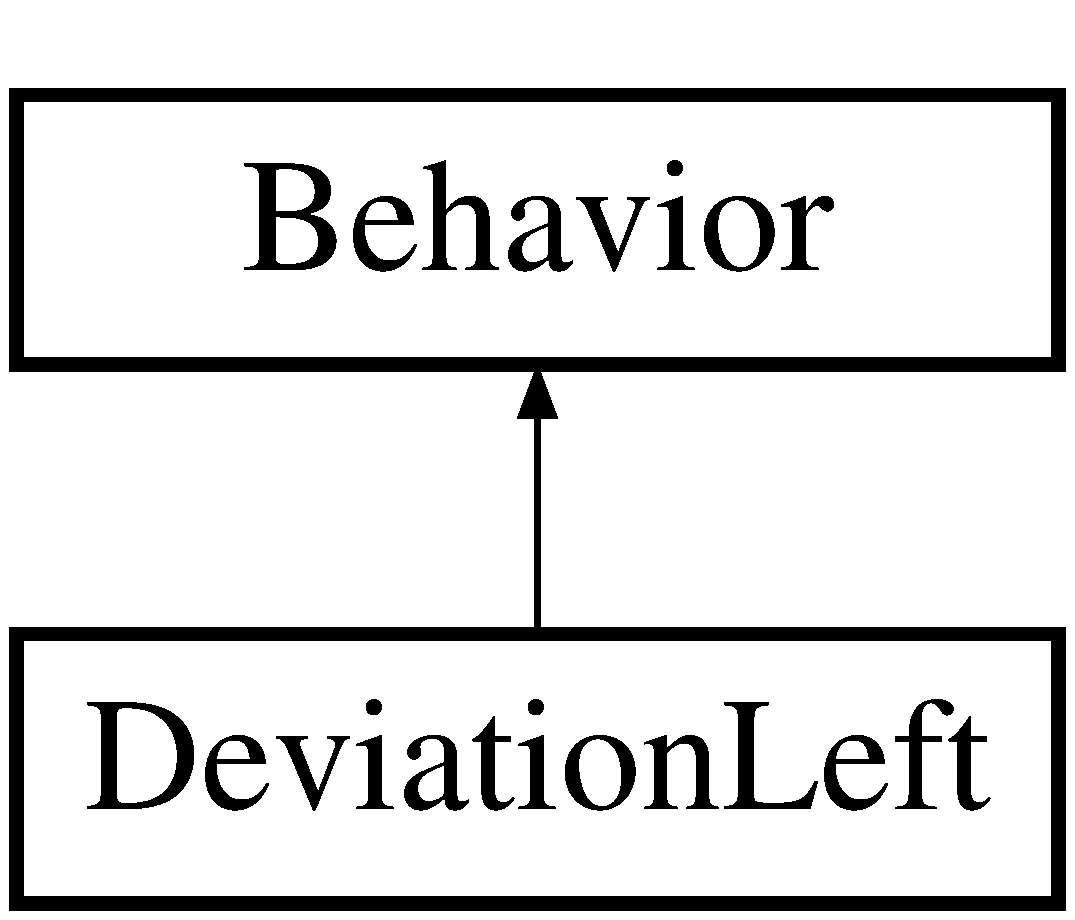
\includegraphics[height=2.000000cm]{class_deviation_left}
\end{center}
\end{figure}
\subsection*{Fonctions membres publiques}
{\bf }\par
\begin{DoxyCompactItemize}
\item 
\hyperlink{class_deviation_left_a6c4ca52d7b6eb31d57bf53c43939b644}{Deviation\-Left} (\hyperlink{class_behavior_context}{Behavior\-Context} $\ast$context)
\begin{DoxyCompactList}\small\item\em Constructeur. \end{DoxyCompactList}\item 
void \hyperlink{class_deviation_left_af11b0c3d1d3d8bf0685ad36ddbd35657}{do\-Action} () override
\begin{DoxyCompactList}\small\item\em Effectue une etape de son comportement. \end{DoxyCompactList}\end{DoxyCompactItemize}

\subsection*{Membres hérités additionnels}


\subsection{Description détaillée}
Classe Etat du comportement \char`\"{}\-Déviation vers la gauche\char`\"{}. 

\subsection{Documentation des constructeurs et destructeur}
\hypertarget{class_deviation_left_a6c4ca52d7b6eb31d57bf53c43939b644}{\index{Deviation\-Left@{Deviation\-Left}!Deviation\-Left@{Deviation\-Left}}
\index{Deviation\-Left@{Deviation\-Left}!DeviationLeft@{Deviation\-Left}}
\subsubsection[{Deviation\-Left}]{\setlength{\rightskip}{0pt plus 5cm}Deviation\-Left\-::\-Deviation\-Left (
\begin{DoxyParamCaption}
\item[{{\bf Behavior\-Context} $\ast$}]{context}
\end{DoxyParamCaption}
)}}\label{class_deviation_left_a6c4ca52d7b6eb31d57bf53c43939b644}


Constructeur. 

Constructeur


\begin{DoxyParams}[1]{Paramètres}
\mbox{\tt in}  & {\em context} & \-: La classe pouvant accéder au robot.\\
\hline
\end{DoxyParams}
\begin{DoxyReturn}{Renvoie}
Aucune. 
\end{DoxyReturn}


\subsection{Documentation des fonctions membres}
\hypertarget{class_deviation_left_af11b0c3d1d3d8bf0685ad36ddbd35657}{\index{Deviation\-Left@{Deviation\-Left}!do\-Action@{do\-Action}}
\index{do\-Action@{do\-Action}!DeviationLeft@{Deviation\-Left}}
\subsubsection[{do\-Action}]{\setlength{\rightskip}{0pt plus 5cm}void Deviation\-Left\-::do\-Action (
\begin{DoxyParamCaption}
{}
\end{DoxyParamCaption}
)\hspace{0.3cm}{\ttfamily [override]}, {\ttfamily [virtual]}}}\label{class_deviation_left_af11b0c3d1d3d8bf0685ad36ddbd35657}


Effectue une etape de son comportement. 

Cette fonction effectue le comportement de l'état actuel.


\begin{DoxyParams}[1]{Paramètres}
\mbox{\tt in}  & {\em Aucun.} & \\
\hline
\end{DoxyParams}
\begin{DoxyReturn}{Renvoie}
Aucune. 
\end{DoxyReturn}


Réimplémentée à partir de \hyperlink{group__inf2990_gac22f205bc85075ff707ad1f695c18439}{Behavior}.



La documentation de cette classe a été générée à partir des fichiers suivants \-:\begin{DoxyCompactItemize}
\item 
C\-:/\-Users/saron/\-Documents/inf2990-\/01/\-Sources/\-D\-L\-L/\-Behavior/\hyperlink{_deviation_left_8h}{Deviation\-Left.\-h}\item 
C\-:/\-Users/saron/\-Documents/inf2990-\/01/\-Sources/\-D\-L\-L/\-Behavior/\hyperlink{_deviation_left_8cpp}{Deviation\-Left.\-cpp}\end{DoxyCompactItemize}

\hypertarget{class_deviation_right}{\section{Référence de la classe Deviation\-Right}
\label{class_deviation_right}\index{Deviation\-Right@{Deviation\-Right}}
}


Classe Etat du comportement \char`\"{}\-Déviation vers la droite\char`\"{}.  




{\ttfamily \#include $<$Deviation\-Right.\-h$>$}

Graphe d'héritage de Deviation\-Right\-:\begin{figure}[H]
\begin{center}
\leavevmode
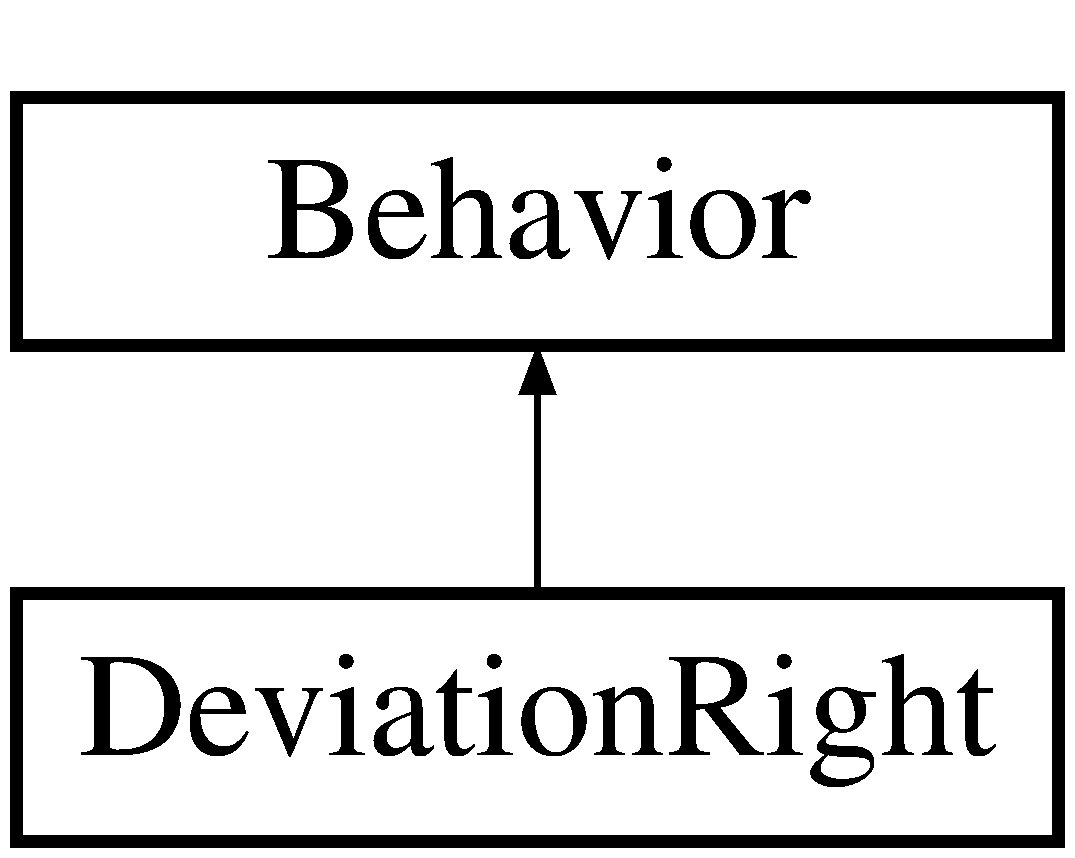
\includegraphics[height=2.000000cm]{class_deviation_right}
\end{center}
\end{figure}
\subsection*{Fonctions membres publiques}
{\bf }\par
\begin{DoxyCompactItemize}
\item 
\hyperlink{class_deviation_right_a022583d0e7a46e3c130994c9aecc12e5}{Deviation\-Right} (\hyperlink{class_behavior_context}{Behavior\-Context} $\ast$context)
\begin{DoxyCompactList}\small\item\em Constructeur. \end{DoxyCompactList}\item 
void \hyperlink{class_deviation_right_a98734577f0efa5672412f410c3dbc551}{do\-Action} () override
\begin{DoxyCompactList}\small\item\em Effectue une etape de son comportement. \end{DoxyCompactList}\end{DoxyCompactItemize}

\subsection*{Membres hérités additionnels}


\subsection{Description détaillée}
Classe Etat du comportement \char`\"{}\-Déviation vers la droite\char`\"{}. 

\subsection{Documentation des constructeurs et destructeur}
\hypertarget{class_deviation_right_a022583d0e7a46e3c130994c9aecc12e5}{\index{Deviation\-Right@{Deviation\-Right}!Deviation\-Right@{Deviation\-Right}}
\index{Deviation\-Right@{Deviation\-Right}!DeviationRight@{Deviation\-Right}}
\subsubsection[{Deviation\-Right}]{\setlength{\rightskip}{0pt plus 5cm}Deviation\-Right\-::\-Deviation\-Right (
\begin{DoxyParamCaption}
\item[{{\bf Behavior\-Context} $\ast$}]{context}
\end{DoxyParamCaption}
)}}\label{class_deviation_right_a022583d0e7a46e3c130994c9aecc12e5}


Constructeur. 

Constructeur


\begin{DoxyParams}[1]{Paramètres}
\mbox{\tt in}  & {\em context} & \-: La classe pouvant accéder au robot.\\
\hline
\end{DoxyParams}
\begin{DoxyReturn}{Renvoie}
Aucune. 
\end{DoxyReturn}


\subsection{Documentation des fonctions membres}
\hypertarget{class_deviation_right_a98734577f0efa5672412f410c3dbc551}{\index{Deviation\-Right@{Deviation\-Right}!do\-Action@{do\-Action}}
\index{do\-Action@{do\-Action}!DeviationRight@{Deviation\-Right}}
\subsubsection[{do\-Action}]{\setlength{\rightskip}{0pt plus 5cm}void Deviation\-Right\-::do\-Action (
\begin{DoxyParamCaption}
{}
\end{DoxyParamCaption}
)\hspace{0.3cm}{\ttfamily [override]}, {\ttfamily [virtual]}}}\label{class_deviation_right_a98734577f0efa5672412f410c3dbc551}


Effectue une etape de son comportement. 

Cette fonction effectue le comportement de l'état actuel.


\begin{DoxyParams}[1]{Paramètres}
\mbox{\tt in}  & {\em Aucun.} & \\
\hline
\end{DoxyParams}
\begin{DoxyReturn}{Renvoie}
Aucune. 
\end{DoxyReturn}


Réimplémentée à partir de \hyperlink{group__inf2990_gac22f205bc85075ff707ad1f695c18439}{Behavior}.



La documentation de cette classe a été générée à partir des fichiers suivants \-:\begin{DoxyCompactItemize}
\item 
C\-:/\-Users/saron/\-Documents/inf2990-\/01/\-Sources/\-D\-L\-L/\-Behavior/\hyperlink{_deviation_right_8h}{Deviation\-Right.\-h}\item 
C\-:/\-Users/saron/\-Documents/inf2990-\/01/\-Sources/\-D\-L\-L/\-Behavior/\hyperlink{_deviation_right_8cpp}{Deviation\-Right.\-cpp}\end{DoxyCompactItemize}

\hypertarget{classmath_1_1_droite3_d}{}\section{math\+:\+:Droite3\+D Class Reference}
\label{classmath_1_1_droite3_d}\index{math\+::\+Droite3\+D@{math\+::\+Droite3\+D}}


Classe qui représente une droite en 3 dimensions.  




{\ttfamily \#include $<$Droite3\+D.\+h$>$}

\subsection*{Public Member Functions}
\begin{DoxyCompactItemize}
\item 
\hyperlink{classmath_1_1_droite3_d_a9248463117b4567a6e68a88f5760f07a}{Droite3\+D} (const glm\+::dvec3 \&point1, const glm\+::dvec3 \&point2)
\begin{DoxyCompactList}\small\item\em Constructeur. \end{DoxyCompactList}\item 
bool \hyperlink{classmath_1_1_droite3_d_acec61f69291777c83e5539fedb83b170}{intersection} (const \hyperlink{classmath_1_1_plan3_d}{Plan3\+D} \&plan\+Coupe, glm\+::dvec3 \&intersection)
\begin{DoxyCompactList}\small\item\em Trouve l\textquotesingle{}intersection entre la droite et un plan. \end{DoxyCompactList}\item 
bool \hyperlink{classmath_1_1_droite3_d_a537d2c35e8ae11d2968087599b10c752}{intersection\+Segment} (const glm\+::dvec3 \&point1, const glm\+::dvec3 \&point2)
\begin{DoxyCompactList}\small\item\em Trouve l\textquotesingle{}intersection entre la droite et un segment. \end{DoxyCompactList}\item 
double \hyperlink{classmath_1_1_droite3_d_a92d2f79fc5d29ddd8061ebb632293f04}{distance\+Point} (const glm\+::dvec3 \&centre)
\begin{DoxyCompactList}\small\item\em Calcule la distance entre un point et la droite. \end{DoxyCompactList}\item 
glm\+::dvec3 \hyperlink{classmath_1_1_droite3_d_a4f3a9fb81926f775cd9e589c112c51db}{perpendiculaire\+Droite} (const glm\+::dvec3 \&point)
\begin{DoxyCompactList}\small\item\em Trouve le point de rencontre entre la droite et une perpendiculaire à partir d\textquotesingle{}un point. \end{DoxyCompactList}\item 
const glm\+::dvec3 \& \hyperlink{classmath_1_1_droite3_d_a903f20fd767699e95f747b4722e8aa04}{lire\+Vecteur} () const 
\begin{DoxyCompactList}\small\item\em Avoir le vecteur directeur de la droite. \end{DoxyCompactList}\item 
const glm\+::dvec3 \& \hyperlink{classmath_1_1_droite3_d_a5de95860b960b37e4c55f857f020c652}{lire\+Point} () const 
\begin{DoxyCompactList}\small\item\em Avoir un point de la droite. \end{DoxyCompactList}\end{DoxyCompactItemize}


\subsection{Detailed Description}
Classe qui représente une droite en 3 dimensions. 

Classe qui permet d\textquotesingle{}avoir une droite en 3\+D. ~\newline
Une droite dans l\textquotesingle{}espace 3\+D est définie par l\textquotesingle{}équation \+:

\[ \frac {x - x_0 } {a} = \frac { y - y_0 } {b} = \frac { z - z_0 } {c} \] où le point $ (x_0, y_0, z_0) $ est un point de la droite et le vecteur de direction $ (a, b, c) $ est un vecteur parallèle à la droite.~\newline
 ~\newline
Une droite dans l\textquotesingle{}espace 3\+D passant par 2 points $ ( P_1, P_2) $ est définie par l\textquotesingle{}équation \+:

\[ \frac {x - x_1 } {x_2 - x_1} = \frac { y - y_1 } {y_2 - y_1} = \frac { z - z_1 } {z_2 - z_1} \] ~\newline
~\newline
Cette classe contient des méthodes pour \+: \begin{DoxyItemize}
\item construire une droite entre 2 points $ (P_1, P_2) $ ou avec un point $ P $ sur la droite et un vecteur de direction $ (a, b, c) $; \item trouver l\textquotesingle{}intersection entre une droite et un plan ; \item intersection\+Segment ; \item distance\+Point ; \item perpendiculaire\+Droite; \item les méthodes d\textquotesingle{}accès.\end{DoxyItemize}
\begin{DoxyAuthor}{Author}
D\+G\+I-\/2990 
\end{DoxyAuthor}
\begin{DoxyDate}{Date}
2005-\/09-\/27 
\end{DoxyDate}


\subsection{Constructor \& Destructor Documentation}
\hypertarget{classmath_1_1_droite3_d_a9248463117b4567a6e68a88f5760f07a}{}\index{math\+::\+Droite3\+D@{math\+::\+Droite3\+D}!Droite3\+D@{Droite3\+D}}
\index{Droite3\+D@{Droite3\+D}!math\+::\+Droite3\+D@{math\+::\+Droite3\+D}}
\subsubsection[{Droite3\+D(const glm\+::dvec3 \&point1, const glm\+::dvec3 \&point2)}]{\setlength{\rightskip}{0pt plus 5cm}math\+::\+Droite3\+D\+::\+Droite3\+D (
\begin{DoxyParamCaption}
\item[{const glm\+::dvec3 \&}]{point1, }
\item[{const glm\+::dvec3 \&}]{point2}
\end{DoxyParamCaption}
)}\label{classmath_1_1_droite3_d_a9248463117b4567a6e68a88f5760f07a}


Constructeur. 

Constructeur d\textquotesingle{}une droite 3\+D à partir de 2 points. ~\newline
Une droite dans l\textquotesingle{}espace 3d passant par 2 points $ ( P_1, P_2) $ est définie par l\textquotesingle{}équation \+:

\[ \frac {x - x_1 } {x_2 - x_1} = \frac { y - y_1 } {y_2 - y_1} = \frac { z - z_1 } {z_2 - z_1} \] ~\newline
~\newline
 
\begin{DoxyParams}[1]{Parameters}
\mbox{\tt in}  & {\em point1} & \+: Un point sur la droite. \\
\hline
\mbox{\tt in}  & {\em point2} & \+: Un autre point sur la droite (différent du premier sinon il y a une levée d\textquotesingle{}exception).\\
\hline
\end{DoxyParams}
\begin{DoxyReturn}{Returns}
Aucune (constructeur). 
\end{DoxyReturn}


\subsection{Member Function Documentation}
\hypertarget{classmath_1_1_droite3_d_a92d2f79fc5d29ddd8061ebb632293f04}{}\index{math\+::\+Droite3\+D@{math\+::\+Droite3\+D}!distance\+Point@{distance\+Point}}
\index{distance\+Point@{distance\+Point}!math\+::\+Droite3\+D@{math\+::\+Droite3\+D}}
\subsubsection[{distance\+Point(const glm\+::dvec3 \&centre)}]{\setlength{\rightskip}{0pt plus 5cm}double math\+::\+Droite3\+D\+::distance\+Point (
\begin{DoxyParamCaption}
\item[{const glm\+::dvec3 \&}]{centre}
\end{DoxyParamCaption}
)}\label{classmath_1_1_droite3_d_a92d2f79fc5d29ddd8061ebb632293f04}


Calcule la distance entre un point et la droite. 

Calcule la distance euclidienne entre la droite et un point.


\begin{DoxyParams}[1]{Parameters}
\mbox{\tt in}  & {\em centre} & \+: Point à partir duquel la distance doit être calculée.\\
\hline
\end{DoxyParams}
\begin{DoxyReturn}{Returns}
Distance du point à la droite. 
\end{DoxyReturn}
\hypertarget{classmath_1_1_droite3_d_acec61f69291777c83e5539fedb83b170}{}\index{math\+::\+Droite3\+D@{math\+::\+Droite3\+D}!intersection@{intersection}}
\index{intersection@{intersection}!math\+::\+Droite3\+D@{math\+::\+Droite3\+D}}
\subsubsection[{intersection(const Plan3\+D \&plan\+Coupe, glm\+::dvec3 \&intersection)}]{\setlength{\rightskip}{0pt plus 5cm}bool math\+::\+Droite3\+D\+::intersection (
\begin{DoxyParamCaption}
\item[{const {\bf Plan3\+D} \&}]{plan\+Coupe, }
\item[{glm\+::dvec3 \&}]{intersection}
\end{DoxyParamCaption}
)}\label{classmath_1_1_droite3_d_acec61f69291777c83e5539fedb83b170}


Trouve l\textquotesingle{}intersection entre la droite et un plan. 

Cette fonction permet de trouver l\textquotesingle{}intersection entre une droite et un plan dans l\textquotesingle{}espace 3\+D. La droite ne doit pas être parallèle au plan. ~\newline
 Si $ a $ est différent de zéro, alors l\textquotesingle{}intersection est donnée par \+:~\newline
 \[ x = \left ( { \frac {\left ( \frac { ( B b + C c) x_0} {a} - B y_0 - C z_0 - D \right)} { ( A + B \frac {b} {a} + C \frac{c} {b})} }\right) \] \[ y = \left ( { \frac {\left ( C \frac {c}{b} y_0 - C z_0 - D \right)} { ( B + C \frac {c} {b}) } }\right) \] \[ z = \frac{c} {a} (x - x_0) + z_0 \]

Si $ b $ est différent de zéro, alors l\textquotesingle{}intersection est donnée par \+:~\newline
 \[ x = x_0 \] \[ y = \frac{c} {b} (x - x_0) + y_0 \] \[ z = \frac{c} {b} (y - y_0) + z_0 \]

Sinon, l\textquotesingle{}intersection est donnée par \+:~\newline
 \[ x = x_0 \] \[ y = y_0 \] \[ z = \frac{(D + A x_0 + B y_0)} {C} \]


\begin{DoxyParams}[1]{Parameters}
\mbox{\tt in}  & {\em plan\+Coupe} & \+: Le plan avec lequel on veut trouver l\textquotesingle{}intersection. \\
\hline
\mbox{\tt out}  & {\em intersection} & \+: Le résultat de l\textquotesingle{}intersection $ (s, y, z) $ .\\
\hline
\end{DoxyParams}
\begin{DoxyReturn}{Returns}
Faux si la droite est parallèle au plan, donc si donc l\textquotesingle{}intersection ne peut être trouvée, vrai autrement. 
\end{DoxyReturn}
\hypertarget{classmath_1_1_droite3_d_a537d2c35e8ae11d2968087599b10c752}{}\index{math\+::\+Droite3\+D@{math\+::\+Droite3\+D}!intersection\+Segment@{intersection\+Segment}}
\index{intersection\+Segment@{intersection\+Segment}!math\+::\+Droite3\+D@{math\+::\+Droite3\+D}}
\subsubsection[{intersection\+Segment(const glm\+::dvec3 \&point1, const glm\+::dvec3 \&point2)}]{\setlength{\rightskip}{0pt plus 5cm}bool math\+::\+Droite3\+D\+::intersection\+Segment (
\begin{DoxyParamCaption}
\item[{const glm\+::dvec3 \&}]{point1, }
\item[{const glm\+::dvec3 \&}]{point2}
\end{DoxyParamCaption}
)}\label{classmath_1_1_droite3_d_a537d2c35e8ae11d2968087599b10c752}


Trouve l\textquotesingle{}intersection entre la droite et un segment. 

Cette fonction permet de trouver l\textquotesingle{}intersection entre un segment de droite défini par 2 points $ (P_1, P_2) $ et une droite dans l\textquotesingle{}espace 3\+D.


\begin{DoxyParams}[1]{Parameters}
\mbox{\tt in}  & {\em point1} & \+: Le premier point du segment. \\
\hline
\mbox{\tt in}  & {\em point2} & \+: Le deuxième point permettant de définir le segment de droite.\\
\hline
\end{DoxyParams}
\begin{DoxyReturn}{Returns}
bool \+: false =$>$ la droite est parallèle au plan, donc l\textquotesingle{}intersection ne peut être trouvée.
\end{DoxyReturn}
\begin{DoxyDate}{Date}
2006-\/02-\/21 Modification suite aux changements dans Vecteur3 
\end{DoxyDate}
\hypertarget{classmath_1_1_droite3_d_a5de95860b960b37e4c55f857f020c652}{}\index{math\+::\+Droite3\+D@{math\+::\+Droite3\+D}!lire\+Point@{lire\+Point}}
\index{lire\+Point@{lire\+Point}!math\+::\+Droite3\+D@{math\+::\+Droite3\+D}}
\subsubsection[{lire\+Point() const }]{\setlength{\rightskip}{0pt plus 5cm}const glm\+::dvec3 \& math\+::\+Droite3\+D\+::lire\+Point (
\begin{DoxyParamCaption}
{}
\end{DoxyParamCaption}
) const\hspace{0.3cm}{\ttfamily [inline]}}\label{classmath_1_1_droite3_d_a5de95860b960b37e4c55f857f020c652}


Avoir un point de la droite. 

Cette fonction retourne un point quelconque de la droite.

\begin{DoxyReturn}{Returns}
Un point quelconque de la droite. 
\end{DoxyReturn}
\hypertarget{classmath_1_1_droite3_d_a903f20fd767699e95f747b4722e8aa04}{}\index{math\+::\+Droite3\+D@{math\+::\+Droite3\+D}!lire\+Vecteur@{lire\+Vecteur}}
\index{lire\+Vecteur@{lire\+Vecteur}!math\+::\+Droite3\+D@{math\+::\+Droite3\+D}}
\subsubsection[{lire\+Vecteur() const }]{\setlength{\rightskip}{0pt plus 5cm}const glm\+::dvec3 \& math\+::\+Droite3\+D\+::lire\+Vecteur (
\begin{DoxyParamCaption}
{}
\end{DoxyParamCaption}
) const\hspace{0.3cm}{\ttfamily [inline]}}\label{classmath_1_1_droite3_d_a903f20fd767699e95f747b4722e8aa04}


Avoir le vecteur directeur de la droite. 

Cette fonction retourne le vecteur directeur de la droite.

\begin{DoxyReturn}{Returns}
Le vecteur directeur de la droite. 
\end{DoxyReturn}
\hypertarget{classmath_1_1_droite3_d_a4f3a9fb81926f775cd9e589c112c51db}{}\index{math\+::\+Droite3\+D@{math\+::\+Droite3\+D}!perpendiculaire\+Droite@{perpendiculaire\+Droite}}
\index{perpendiculaire\+Droite@{perpendiculaire\+Droite}!math\+::\+Droite3\+D@{math\+::\+Droite3\+D}}
\subsubsection[{perpendiculaire\+Droite(const glm\+::dvec3 \&point)}]{\setlength{\rightskip}{0pt plus 5cm}glm\+::dvec3 math\+::\+Droite3\+D\+::perpendiculaire\+Droite (
\begin{DoxyParamCaption}
\item[{const glm\+::dvec3 \&}]{point}
\end{DoxyParamCaption}
)}\label{classmath_1_1_droite3_d_a4f3a9fb81926f775cd9e589c112c51db}


Trouve le point de rencontre entre la droite et une perpendiculaire à partir d\textquotesingle{}un point. 

On trace la perpendicaulaire entre le point et le droite et on trouve le point d\textquotesingle{}intersection.


\begin{DoxyParams}[1]{Parameters}
\mbox{\tt in}  & {\em point} & \+: Un point dans l\textquotesingle{}espace d\textquotesingle{}où est calculée la perpendiculaire.\\
\hline
\end{DoxyParams}
\begin{DoxyReturn}{Returns}
Le point de rencontre entre la droite et la perpendiculaire. 
\end{DoxyReturn}


The documentation for this class was generated from the following files\+:\begin{DoxyCompactItemize}
\item 
C\+:/\+Users/\+Louis/workspace/inf2990-\/01/\+Commun/\+Utilitaire/\hyperlink{_droite3_d_8h}{Droite3\+D.\+h}\item 
C\+:/\+Users/\+Louis/workspace/inf2990-\/01/\+Commun/\+Utilitaire/\hyperlink{_droite3_d_8cpp}{Droite3\+D.\+cpp}\end{DoxyCompactItemize}

\hypertarget{class_droite3_d_test}{\section{Référence de la classe Droite3\-D\-Test}
\label{class_droite3_d_test}\index{Droite3\-D\-Test@{Droite3\-D\-Test}}
}


Classe de test cppunit pour tester le bon fonctionnement des méthodes de la classe Droite3\-D.  




{\ttfamily \#include $<$Droite3\-D\-Test.\-h$>$}

Graphe d'héritage de Droite3\-D\-Test\-:\begin{figure}[H]
\begin{center}
\leavevmode
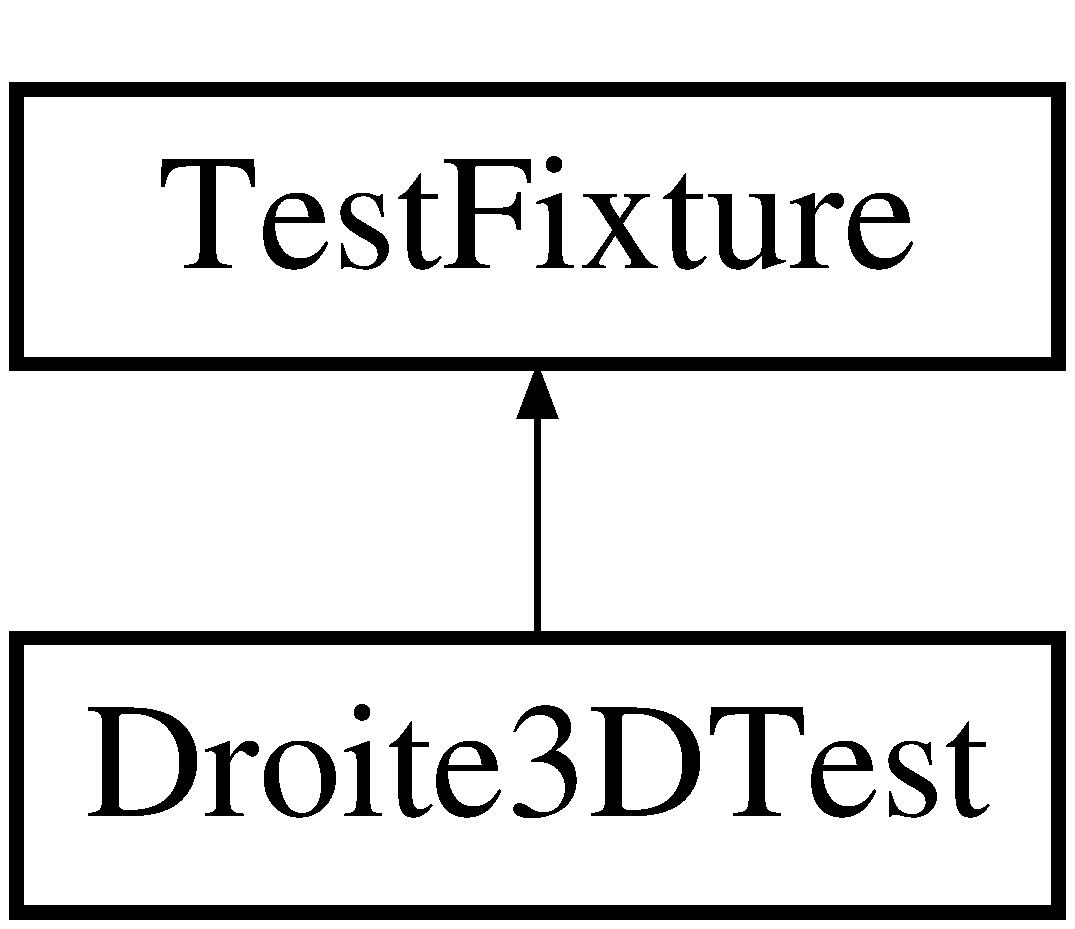
\includegraphics[height=2.000000cm]{class_droite3_d_test}
\end{center}
\end{figure}
\subsection*{Fonctions membres publiques}
\begin{DoxyCompactItemize}
\item 
void \hyperlink{group__inf2990_ga2058c915e823fa8ab26bad2c22554565}{set\-Up} ()
\begin{DoxyCompactList}\small\item\em Traitement à effectuer pour initialiser cette suite de tests. \end{DoxyCompactList}\item 
void \hyperlink{group__inf2990_gac9305147cf292b41834fabd24e57b976}{tear\-Down} ()
\begin{DoxyCompactList}\small\item\em Traitement à effectuer pour 'finaliser' cette suite de tests. \end{DoxyCompactList}\item 
void \hyperlink{group__inf2990_gaeae69515feaa3c448b7489289910c467}{test\-Vecteur} ()
\begin{DoxyCompactList}\small\item\em Cas de test\-: vecteur directeur de la droite. \end{DoxyCompactList}\item 
void \hyperlink{group__inf2990_gaa99e4b9c5f0916cef3b8dfe7ab8a4e9d}{test\-Intersection} ()
\begin{DoxyCompactList}\small\item\em Cas de test\-: intersection entre deux droites. \end{DoxyCompactList}\end{DoxyCompactItemize}


\subsection{Description détaillée}
Classe de test cppunit pour tester le bon fonctionnement des méthodes de la classe Droite3\-D. 

\begin{DoxyAuthor}{Auteur}
I\-N\-F2990-\/\-A15-\/01 
\end{DoxyAuthor}
\begin{DoxyDate}{Date}
2015-\/11-\/06 
\end{DoxyDate}


La documentation de cette classe a été générée à partir des fichiers suivants \-:\begin{DoxyCompactItemize}
\item 
C\-:/\-Users/saron/\-Documents/inf2990-\/01/\-Sources/\-D\-L\-L/\-Tests/Droite3\-D\-Test.\-h\item 
C\-:/\-Users/saron/\-Documents/inf2990-\/01/\-Sources/\-D\-L\-L/\-Tests/Droite3\-D\-Test.\-cpp\end{DoxyCompactItemize}

\hypertarget{class_interface_graphique_1_1_tools_1_1_duplicate}{\section{Référence de la classe Interface\-Graphique.\-Tools.\-Duplicate}
\label{class_interface_graphique_1_1_tools_1_1_duplicate}\index{Interface\-Graphique.\-Tools.\-Duplicate@{Interface\-Graphique.\-Tools.\-Duplicate}}
}


Représente l'outil de duplication.  


Graphe d'héritage de Interface\-Graphique.\-Tools.\-Duplicate\-:\begin{figure}[H]
\begin{center}
\leavevmode
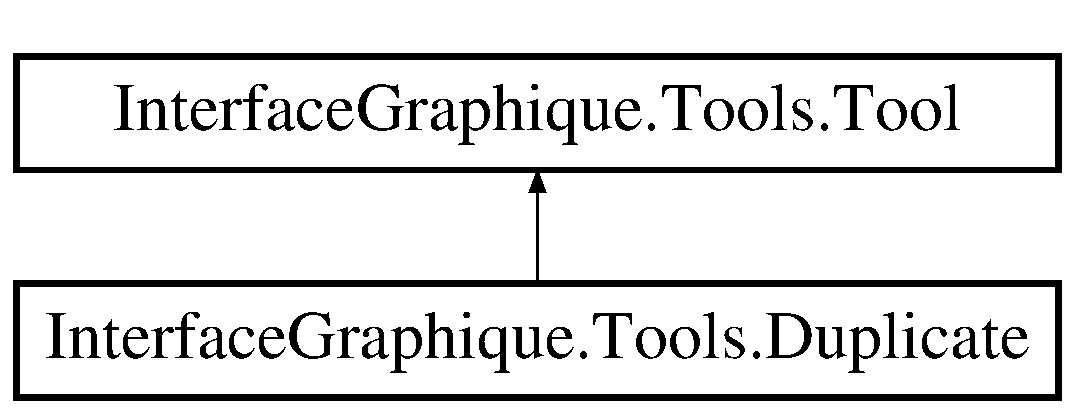
\includegraphics[height=2.000000cm]{class_interface_graphique_1_1_tools_1_1_duplicate}
\end{center}
\end{figure}
\subsection*{Fonctions membres publiques}
\begin{DoxyCompactItemize}
\item 
\hypertarget{class_interface_graphique_1_1_tools_1_1_duplicate_a4537f9c39028b8e04820cb054f7d8ffa}{{\bfseries Duplicate} (\hyperlink{class_interface_graphique_1_1_tools_1_1_tool_context}{Tool\-Context} context, \hyperlink{class_interface_graphique_1_1_engine}{Engine} \-\_\-engine)}\label{class_interface_graphique_1_1_tools_1_1_duplicate_a4537f9c39028b8e04820cb054f7d8ffa}

\item 
override void \hyperlink{class_interface_graphique_1_1_tools_1_1_duplicate_ab3771a3f6ead534124feaf89f542a910}{Left\-Mouse\-Pressed} (Mouse\-Event\-Args e)
\item 
override void \hyperlink{class_interface_graphique_1_1_tools_1_1_duplicate_a23482008d3d07f80d4b5b9db77fd63c9}{Left\-Mouse\-Released} (Mouse\-Event\-Args e)
\item 
override void \hyperlink{class_interface_graphique_1_1_tools_1_1_duplicate_a55a29f559ad9051390f107b34cd667a6}{Left\-Mouse\-Full\-Clicked} (Mouse\-Event\-Args e)
\item 
override void \hyperlink{class_interface_graphique_1_1_tools_1_1_duplicate_a92888a92cbdd84f7c617b82dde014c0f}{Dragging} (int delta\-X, int delta\-Y, int delta\-Z)
\item 
override void \hyperlink{class_interface_graphique_1_1_tools_1_1_duplicate_aa8bb7b1bf21dceacd60ac1a502c31a40}{Mouse\-Move} (Mouse\-Event\-Args e)
\item 
override void \hyperlink{class_interface_graphique_1_1_tools_1_1_duplicate_a52769869afe558c10ec13bbc54d896f3}{esc} ()
\end{DoxyCompactItemize}
\subsection*{Membres hérités additionnels}


\subsection{Description détaillée}
Représente l'outil de duplication. 

\begin{DoxyAuthor}{Auteur}
I\-N\-F2990-\/\-A15-\/01 
\end{DoxyAuthor}
\begin{DoxyDate}{Date}
2015-\/10-\/01 
\end{DoxyDate}


\subsection{Documentation des fonctions membres}
\hypertarget{class_interface_graphique_1_1_tools_1_1_duplicate_a92888a92cbdd84f7c617b82dde014c0f}{\index{Interface\-Graphique\-::\-Tools\-::\-Duplicate@{Interface\-Graphique\-::\-Tools\-::\-Duplicate}!Dragging@{Dragging}}
\index{Dragging@{Dragging}!InterfaceGraphique::Tools::Duplicate@{Interface\-Graphique\-::\-Tools\-::\-Duplicate}}
\subsubsection[{Dragging}]{\setlength{\rightskip}{0pt plus 5cm}override void Interface\-Graphique.\-Tools.\-Duplicate.\-Dragging (
\begin{DoxyParamCaption}
\item[{int}]{delta\-X, }
\item[{int}]{delta\-Y, }
\item[{int}]{delta\-Z}
\end{DoxyParamCaption}
)\hspace{0.3cm}{\ttfamily [inline]}, {\ttfamily [virtual]}}}\label{class_interface_graphique_1_1_tools_1_1_duplicate_a92888a92cbdd84f7c617b82dde014c0f}
Appelé dès qu'on bouge des éléments


\begin{DoxyParams}[1]{Paramètres}
\mbox{\tt in}  & {\em delta\-X} & \-: la distance en X \\
\hline
\mbox{\tt in}  & {\em delta\-Y} & \-: la distance en Y \\
\hline
\mbox{\tt in}  & {\em delta\-Z} & \-: la distance en Z\\
\hline
\end{DoxyParams}
\begin{DoxyReturn}{Renvoie}
Aucun 
\end{DoxyReturn}


Réimplémentée à partir de \hyperlink{class_interface_graphique_1_1_tools_1_1_tool_a8b9595e6a3eb55443b8b2cdb38a2c390}{Interface\-Graphique.\-Tools.\-Tool}.

\hypertarget{class_interface_graphique_1_1_tools_1_1_duplicate_a52769869afe558c10ec13bbc54d896f3}{\index{Interface\-Graphique\-::\-Tools\-::\-Duplicate@{Interface\-Graphique\-::\-Tools\-::\-Duplicate}!esc@{esc}}
\index{esc@{esc}!InterfaceGraphique::Tools::Duplicate@{Interface\-Graphique\-::\-Tools\-::\-Duplicate}}
\subsubsection[{esc}]{\setlength{\rightskip}{0pt plus 5cm}override void Interface\-Graphique.\-Tools.\-Duplicate.\-esc (
\begin{DoxyParamCaption}
{}
\end{DoxyParamCaption}
)\hspace{0.3cm}{\ttfamily [inline]}, {\ttfamily [virtual]}}}\label{class_interface_graphique_1_1_tools_1_1_duplicate_a52769869afe558c10ec13bbc54d896f3}
Appelé quand on fait escape

\begin{DoxyReturn}{Renvoie}
Aucun 
\end{DoxyReturn}


Réimplémentée à partir de \hyperlink{class_interface_graphique_1_1_tools_1_1_tool_a734cc3904ce75149652ac356caba93f7}{Interface\-Graphique.\-Tools.\-Tool}.

\hypertarget{class_interface_graphique_1_1_tools_1_1_duplicate_a55a29f559ad9051390f107b34cd667a6}{\index{Interface\-Graphique\-::\-Tools\-::\-Duplicate@{Interface\-Graphique\-::\-Tools\-::\-Duplicate}!Left\-Mouse\-Full\-Clicked@{Left\-Mouse\-Full\-Clicked}}
\index{Left\-Mouse\-Full\-Clicked@{Left\-Mouse\-Full\-Clicked}!InterfaceGraphique::Tools::Duplicate@{Interface\-Graphique\-::\-Tools\-::\-Duplicate}}
\subsubsection[{Left\-Mouse\-Full\-Clicked}]{\setlength{\rightskip}{0pt plus 5cm}override void Interface\-Graphique.\-Tools.\-Duplicate.\-Left\-Mouse\-Full\-Clicked (
\begin{DoxyParamCaption}
\item[{Mouse\-Event\-Args}]{e}
\end{DoxyParamCaption}
)\hspace{0.3cm}{\ttfamily [inline]}, {\ttfamily [virtual]}}}\label{class_interface_graphique_1_1_tools_1_1_duplicate_a55a29f559ad9051390f107b34cd667a6}
Appelé quand on appuis et relâche sur le bouton gauche de la souris à l'intérieur de trois pixels. Représente un click.


\begin{DoxyParams}[1]{Paramètres}
\mbox{\tt in}  & {\em e} & \-: les informations sur l'événement\\
\hline
\end{DoxyParams}
\begin{DoxyReturn}{Renvoie}
Aucun 
\end{DoxyReturn}


Réimplémentée à partir de \hyperlink{class_interface_graphique_1_1_tools_1_1_tool_a043f210d7840ec8aa5723b193e71ead5}{Interface\-Graphique.\-Tools.\-Tool}.

\hypertarget{class_interface_graphique_1_1_tools_1_1_duplicate_ab3771a3f6ead534124feaf89f542a910}{\index{Interface\-Graphique\-::\-Tools\-::\-Duplicate@{Interface\-Graphique\-::\-Tools\-::\-Duplicate}!Left\-Mouse\-Pressed@{Left\-Mouse\-Pressed}}
\index{Left\-Mouse\-Pressed@{Left\-Mouse\-Pressed}!InterfaceGraphique::Tools::Duplicate@{Interface\-Graphique\-::\-Tools\-::\-Duplicate}}
\subsubsection[{Left\-Mouse\-Pressed}]{\setlength{\rightskip}{0pt plus 5cm}override void Interface\-Graphique.\-Tools.\-Duplicate.\-Left\-Mouse\-Pressed (
\begin{DoxyParamCaption}
\item[{Mouse\-Event\-Args}]{e}
\end{DoxyParamCaption}
)\hspace{0.3cm}{\ttfamily [inline]}, {\ttfamily [virtual]}}}\label{class_interface_graphique_1_1_tools_1_1_duplicate_ab3771a3f6ead534124feaf89f542a910}
Appelé quand on appuis sur le bouton gauche de la souris


\begin{DoxyParams}[1]{Paramètres}
\mbox{\tt in}  & {\em e} & \-: les informations sur l'événement\\
\hline
\end{DoxyParams}
\begin{DoxyReturn}{Renvoie}
Aucun 
\end{DoxyReturn}


Réimplémentée à partir de \hyperlink{class_interface_graphique_1_1_tools_1_1_tool_af5c8a4b2773f0d09f45575ade24769ba}{Interface\-Graphique.\-Tools.\-Tool}.

\hypertarget{class_interface_graphique_1_1_tools_1_1_duplicate_a23482008d3d07f80d4b5b9db77fd63c9}{\index{Interface\-Graphique\-::\-Tools\-::\-Duplicate@{Interface\-Graphique\-::\-Tools\-::\-Duplicate}!Left\-Mouse\-Released@{Left\-Mouse\-Released}}
\index{Left\-Mouse\-Released@{Left\-Mouse\-Released}!InterfaceGraphique::Tools::Duplicate@{Interface\-Graphique\-::\-Tools\-::\-Duplicate}}
\subsubsection[{Left\-Mouse\-Released}]{\setlength{\rightskip}{0pt plus 5cm}override void Interface\-Graphique.\-Tools.\-Duplicate.\-Left\-Mouse\-Released (
\begin{DoxyParamCaption}
\item[{Mouse\-Event\-Args}]{e}
\end{DoxyParamCaption}
)\hspace{0.3cm}{\ttfamily [inline]}, {\ttfamily [virtual]}}}\label{class_interface_graphique_1_1_tools_1_1_duplicate_a23482008d3d07f80d4b5b9db77fd63c9}
Appelé quand on relâche sur le bouton gauche de la souris


\begin{DoxyParams}[1]{Paramètres}
\mbox{\tt in}  & {\em e} & \-: les informations sur l'événement\\
\hline
\end{DoxyParams}
\begin{DoxyReturn}{Renvoie}
Aucun 
\end{DoxyReturn}


Réimplémentée à partir de \hyperlink{class_interface_graphique_1_1_tools_1_1_tool_a51c4828f7d24c599b5748b9b3f64d39e}{Interface\-Graphique.\-Tools.\-Tool}.

\hypertarget{class_interface_graphique_1_1_tools_1_1_duplicate_aa8bb7b1bf21dceacd60ac1a502c31a40}{\index{Interface\-Graphique\-::\-Tools\-::\-Duplicate@{Interface\-Graphique\-::\-Tools\-::\-Duplicate}!Mouse\-Move@{Mouse\-Move}}
\index{Mouse\-Move@{Mouse\-Move}!InterfaceGraphique::Tools::Duplicate@{Interface\-Graphique\-::\-Tools\-::\-Duplicate}}
\subsubsection[{Mouse\-Move}]{\setlength{\rightskip}{0pt plus 5cm}override void Interface\-Graphique.\-Tools.\-Duplicate.\-Mouse\-Move (
\begin{DoxyParamCaption}
\item[{Mouse\-Event\-Args}]{e}
\end{DoxyParamCaption}
)\hspace{0.3cm}{\ttfamily [inline]}, {\ttfamily [virtual]}}}\label{class_interface_graphique_1_1_tools_1_1_duplicate_aa8bb7b1bf21dceacd60ac1a502c31a40}
Appelé quand on bouge la souris


\begin{DoxyParams}[1]{Paramètres}
\mbox{\tt in}  & {\em e} & \-: les informations sur l'événement\\
\hline
\end{DoxyParams}
\begin{DoxyReturn}{Renvoie}
Aucun 
\end{DoxyReturn}


Réimplémentée à partir de \hyperlink{class_interface_graphique_1_1_tools_1_1_tool_aedd1c93f96ee602475b7cbc3c9c99baa}{Interface\-Graphique.\-Tools.\-Tool}.



La documentation de cette classe a été générée à partir du fichier suivant \-:\begin{DoxyCompactItemize}
\item 
C\-:/\-Users/saron/\-Documents/inf2990-\/01/\-Sources/\-Interface\-Graphique/\-Tools/Duplicate.\-cs\end{DoxyCompactItemize}

\hypertarget{class_duplicate_tool}{}\section{Duplicate\+Tool Class Reference}
\label{class_duplicate_tool}\index{Duplicate\+Tool@{Duplicate\+Tool}}


Classe concrète héritant de \hyperlink{class_tool}{Tool}, qui effectue l\textquotesingle{}opération de duplication sur un noeud de l\textquotesingle{}arbre de rendu.  




{\ttfamily \#include $<$Duplicate\+Tool.\+h$>$}

Inheritance diagram for Duplicate\+Tool\+:\begin{figure}[H]
\begin{center}
\leavevmode
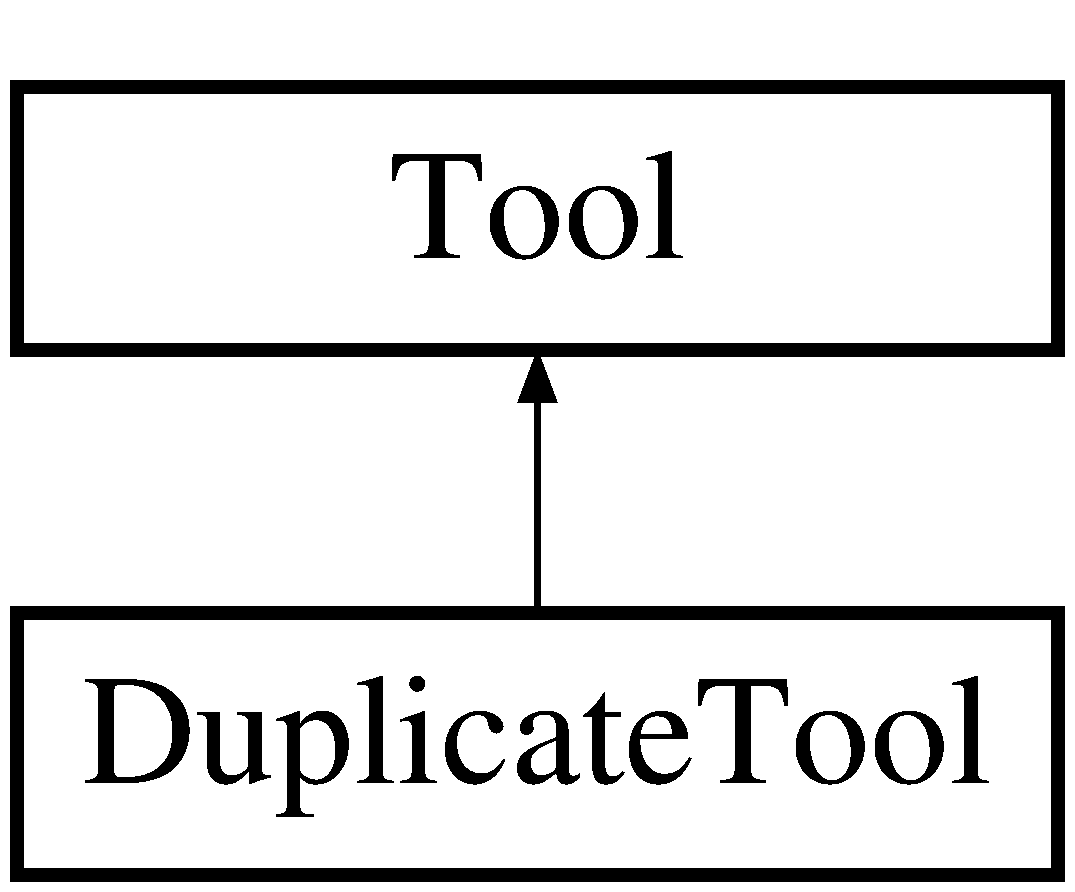
\includegraphics[height=2.000000cm]{class_duplicate_tool}
\end{center}
\end{figure}
\subsection*{Public Member Functions}
\begin{DoxyCompactItemize}
\item 
\hyperlink{group__inf2990_ga13dd0524e005f4a44dbaeea9f237d761}{Duplicate\+Tool} (glm\+::dvec3 center)
\item 
\hyperlink{group__inf2990_gaab141bc62b424e5e0bfc48bd899bcb8a}{$\sim$\+Duplicate\+Tool} ()
\item 
void \hyperlink{group__inf2990_gab91de27487440694048c1a0fbcc74da7}{visit} (\hyperlink{class_noeud_cylindre}{Noeud\+Cylindre} $\ast$node) override
\item 
void \hyperlink{group__inf2990_ga5fa8bbf01a90c95062c8104ebdf5bb62}{visit} (\hyperlink{class_noeud_depart}{Noeud\+Depart} $\ast$node) override
\item 
void \hyperlink{group__inf2990_ga73745cfc31434fbac0697d54aad3f571}{visit} (\hyperlink{class_noeud_ligne}{Noeud\+Ligne} $\ast$node) override
\item 
void \hyperlink{group__inf2990_ga9b9e4456490e59603f3d8924fdf19c18}{visit} (\hyperlink{class_noeud_mur}{Noeud\+Mur} $\ast$node) override
\item 
void \hyperlink{group__inf2990_ga4708caab32b10170d24dba25d4829677}{default\+Duplicate} (\hyperlink{class_noeud_abstrait}{Noeud\+Abstrait} $\ast$node)
\item 
\hypertarget{group__inf2990_gadbe76417e934ddabc6df18141162fe2c}{}void {\bfseries duplicate} ()\label{group__inf2990_gadbe76417e934ddabc6df18141162fe2c}

\item 
void \hyperlink{group__inf2990_ga2fad36673e41afac22177ca37c6c75ff}{update\+Buffer} (glm\+::dvec3 cursor)
\item 
void \hyperlink{group__inf2990_ga69fcbb20577c85049ca9a5ca8b37091d}{confirm\+Buffer} ()
\end{DoxyCompactItemize}


\subsection{Detailed Description}
Classe concrète héritant de \hyperlink{class_tool}{Tool}, qui effectue l\textquotesingle{}opération de duplication sur un noeud de l\textquotesingle{}arbre de rendu. 

\begin{DoxyAuthor}{Author}
I\+N\+F2990-\/\+A15-\/01 
\end{DoxyAuthor}
\begin{DoxyDate}{Date}
2015-\/09-\/14 
\end{DoxyDate}


The documentation for this class was generated from the following files\+:\begin{DoxyCompactItemize}
\item 
Sources/\+D\+L\+L/\+Application/\+Visitor/\hyperlink{_duplicate_tool_8h}{Duplicate\+Tool.\+h}\item 
Sources/\+D\+L\+L/\+Application/\+Visitor/\hyperlink{_duplicate_tool_8cpp}{Duplicate\+Tool.\+cpp}\end{DoxyCompactItemize}

\hypertarget{struct_noeud_mur_1_1dvec3__duo}{\section{Référence de la structure Noeud\-Mur\-:\-:dvec3\-\_\-duo}
\label{struct_noeud_mur_1_1dvec3__duo}\index{Noeud\-Mur\-::dvec3\-\_\-duo@{Noeud\-Mur\-::dvec3\-\_\-duo}}
}


Points du mur.  




{\ttfamily \#include $<$Noeud\-Mur.\-h$>$}

\subsection*{Fonctions membres publiques}
\begin{DoxyCompactItemize}
\item 
\hypertarget{struct_noeud_mur_1_1dvec3__duo_ad463f5add9aebd2a17216d6d6263f275}{{\bfseries dvec3\-\_\-duo} (const glm\-::dvec3 \&p1, const glm\-::dvec3 \&p2)}\label{struct_noeud_mur_1_1dvec3__duo_ad463f5add9aebd2a17216d6d6263f275}

\end{DoxyCompactItemize}
\subsection*{Attributs publics}
\begin{DoxyCompactItemize}
\item 
\hypertarget{struct_noeud_mur_1_1dvec3__duo_aa8b3e1732fd2557fedfe7654e831da99}{glm\-::dvec3 {\bfseries start}}\label{struct_noeud_mur_1_1dvec3__duo_aa8b3e1732fd2557fedfe7654e831da99}

\item 
\hypertarget{struct_noeud_mur_1_1dvec3__duo_a773c7fee621b9ce041792ee7b9e4b9e8}{glm\-::dvec3 {\bfseries end}}\label{struct_noeud_mur_1_1dvec3__duo_a773c7fee621b9ce041792ee7b9e4b9e8}

\end{DoxyCompactItemize}


\subsection{Description détaillée}
Points du mur. 

La documentation de cette structure a été générée à partir du fichier suivant \-:\begin{DoxyCompactItemize}
\item 
C\-:/\-Users/saron/\-Documents/inf2990-\/01/\-Sources/\-D\-L\-L/\-Arbre/\-Noeuds/\hyperlink{_noeud_mur_8h}{Noeud\-Mur.\-h}\end{DoxyCompactItemize}

\hypertarget{class_interface_graphique_1_1_editor}{}\section{Interface\+Graphique.\+Editor Class Reference}
\label{class_interface_graphique_1_1_editor}\index{Interface\+Graphique.\+Editor@{Interface\+Graphique.\+Editor}}


Interaction logic for wpftest.\+xaml  


Inheritance diagram for Interface\+Graphique.\+Editor\+:\begin{figure}[H]
\begin{center}
\leavevmode
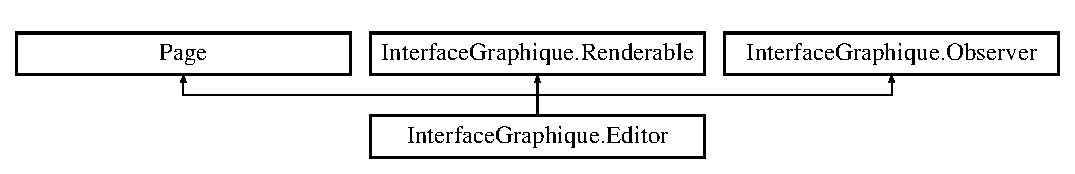
\includegraphics[height=2.000000cm]{class_interface_graphique_1_1_editor}
\end{center}
\end{figure}
\subsection*{Public Member Functions}
\begin{DoxyCompactItemize}
\item 
\hypertarget{class_interface_graphique_1_1_editor_add671582e88cc312606ff0cd8647d9f6}{}delegate void {\bfseries Click\+Event\+Handler} (object sender, Event\+Args e)\label{class_interface_graphique_1_1_editor_add671582e88cc312606ff0cd8647d9f6}

\item 
\hyperlink{class_interface_graphique_1_1_editor_a27b5ab7b3d2e83716e4e6834f9b09931}{Editor} ()
\item 
\hypertarget{class_interface_graphique_1_1_editor_af9417f24c0cfdcbad45e3b0d97556bb3}{}void {\bfseries Frame\+Update} (double temps\+Inter\+Affichage)\label{class_interface_graphique_1_1_editor_af9417f24c0cfdcbad45e3b0d97556bb3}

\item 
\hypertarget{class_interface_graphique_1_1_editor_a725d9e2a16dd2806082660391d9035d4}{}void {\bfseries Zoom\+\_\+\+Rectangle} (object sender, Routed\+Event\+Args e)\label{class_interface_graphique_1_1_editor_a725d9e2a16dd2806082660391d9035d4}

\end{DoxyCompactItemize}
\subsection*{Events}
\begin{DoxyCompactItemize}
\item 
\hypertarget{class_interface_graphique_1_1_editor_a361c2e1a5c98707a168204aab184c23e}{}Click\+Event\+Handler {\bfseries Load\+Main\+Menu}\label{class_interface_graphique_1_1_editor_a361c2e1a5c98707a168204aab184c23e}

\end{DoxyCompactItemize}


\subsection{Detailed Description}
Interaction logic for wpftest.\+xaml 



\subsection{Constructor \& Destructor Documentation}
\hypertarget{class_interface_graphique_1_1_editor_a27b5ab7b3d2e83716e4e6834f9b09931}{}\index{Interface\+Graphique\+::\+Editor@{Interface\+Graphique\+::\+Editor}!Editor@{Editor}}
\index{Editor@{Editor}!Interface\+Graphique\+::\+Editor@{Interface\+Graphique\+::\+Editor}}
\subsubsection[{Editor()}]{\setlength{\rightskip}{0pt plus 5cm}Interface\+Graphique.\+Editor.\+Editor (
\begin{DoxyParamCaption}
{}
\end{DoxyParamCaption}
)\hspace{0.3cm}{\ttfamily [inline]}}\label{class_interface_graphique_1_1_editor_a27b5ab7b3d2e83716e4e6834f9b09931}
Resize on resize only 

The documentation for this class was generated from the following file\+:\begin{DoxyCompactItemize}
\item 
Sources/\+Interface\+Graphique/Editor.\+xaml.\+cs\end{DoxyCompactItemize}

\hypertarget{class_interface_graphique_1_1_editor_controller}{}\section{Interface\+Graphique.\+Editor\+Controller Class Reference}
\label{class_interface_graphique_1_1_editor_controller}\index{Interface\+Graphique.\+Editor\+Controller@{Interface\+Graphique.\+Editor\+Controller}}
\subsection*{Public Member Functions}
\begin{DoxyCompactItemize}
\item 
\hypertarget{class_interface_graphique_1_1_editor_controller_a5dd318fe9ffbc3d4a9515a3c50799f90}{}delegate void {\bfseries Selected\+Event\+Handler} (int nb\+Selected)\label{class_interface_graphique_1_1_editor_controller_a5dd318fe9ffbc3d4a9515a3c50799f90}

\item 
\hypertarget{class_interface_graphique_1_1_editor_controller_aeac82bbe20161320c61ad3d6f6c09439}{}delegate void {\bfseries Node\+Changed\+Event\+Handler} ()\label{class_interface_graphique_1_1_editor_controller_aeac82bbe20161320c61ad3d6f6c09439}

\item 
\hypertarget{class_interface_graphique_1_1_editor_controller_a9e1a8125231bfc91d78a58494eea9b52}{}void {\bfseries Key\+Pressed} (object o, Key\+Event\+Args e)\label{class_interface_graphique_1_1_editor_controller_a9e1a8125231bfc91d78a58494eea9b52}

\item 
\hypertarget{class_interface_graphique_1_1_editor_controller_a012354c95b60c84f57158c79f277f48a}{}void {\bfseries Mouse\+Button\+Down} (Object o, Forms.\+Mouse\+Event\+Args e)\label{class_interface_graphique_1_1_editor_controller_a012354c95b60c84f57158c79f277f48a}

\item 
\hypertarget{class_interface_graphique_1_1_editor_controller_a6d5271f6ddfdec825e50a5a573cc3cd2}{}void {\bfseries Mouse\+Button\+Up} (Object o, Forms.\+Mouse\+Event\+Args e)\label{class_interface_graphique_1_1_editor_controller_a6d5271f6ddfdec825e50a5a573cc3cd2}

\item 
\hypertarget{class_interface_graphique_1_1_editor_controller_a3125ab438e444b57565d9a1df1e47752}{}void {\bfseries Mouse\+Move} (Object o, Forms.\+Mouse\+Event\+Args e)\label{class_interface_graphique_1_1_editor_controller_a3125ab438e444b57565d9a1df1e47752}

\item 
\hypertarget{class_interface_graphique_1_1_editor_controller_a2d2f01230ad526588cc7ad4d7d0654e3}{}void {\bfseries Roulette\+Souris} (Object o, Forms.\+Mouse\+Event\+Args e)\label{class_interface_graphique_1_1_editor_controller_a2d2f01230ad526588cc7ad4d7d0654e3}

\item 
\hypertarget{class_interface_graphique_1_1_editor_controller_ada1b0f4f1183faf2d66a4be4a453da24}{}void {\bfseries Detect\+Drag} ()\label{class_interface_graphique_1_1_editor_controller_ada1b0f4f1183faf2d66a4be4a453da24}

\item 
\hypertarget{class_interface_graphique_1_1_editor_controller_a1c406b266f2129d9199072e5ae866621}{}void {\bfseries Zoom\+In} ()\label{class_interface_graphique_1_1_editor_controller_a1c406b266f2129d9199072e5ae866621}

\item 
\hypertarget{class_interface_graphique_1_1_editor_controller_a94cbbf18cacc71bbca978c9166fe36ee}{}void {\bfseries Zoom\+Out} ()\label{class_interface_graphique_1_1_editor_controller_a94cbbf18cacc71bbca978c9166fe36ee}

\item 
\hypertarget{class_interface_graphique_1_1_editor_controller_a8bd73634e07d893c4c352b5e84643401}{}void {\bfseries create} (string node\+Type)\label{class_interface_graphique_1_1_editor_controller_a8bd73634e07d893c4c352b5e84643401}

\item 
\hypertarget{class_interface_graphique_1_1_editor_controller_a43f1e04a48e49d9ced5d0059952a5d69}{}void {\bfseries translate} ()\label{class_interface_graphique_1_1_editor_controller_a43f1e04a48e49d9ced5d0059952a5d69}

\item 
\hypertarget{class_interface_graphique_1_1_editor_controller_a72358ea2ef1b5f6e747a2f2559152236}{}void {\bfseries select} ()\label{class_interface_graphique_1_1_editor_controller_a72358ea2ef1b5f6e747a2f2559152236}

\item 
\hypertarget{class_interface_graphique_1_1_editor_controller_aa4a297885c6a81332c9516b11388f377}{}void {\bfseries zoom\+Rectangle} ()\label{class_interface_graphique_1_1_editor_controller_aa4a297885c6a81332c9516b11388f377}

\item 
\hypertarget{class_interface_graphique_1_1_editor_controller_ac6b23da8b8749616b321af6c7ed4f536}{}void {\bfseries rotate} ()\label{class_interface_graphique_1_1_editor_controller_ac6b23da8b8749616b321af6c7ed4f536}

\item 
\hypertarget{class_interface_graphique_1_1_editor_controller_ac15c633a9d7b8c2e9dde51a8bde72fab}{}void {\bfseries scale} ()\label{class_interface_graphique_1_1_editor_controller_ac15c633a9d7b8c2e9dde51a8bde72fab}

\item 
\hypertarget{class_interface_graphique_1_1_editor_controller_a404de89ddf6b8418a9a19c0d30b84f77}{}void {\bfseries duplicate} ()\label{class_interface_graphique_1_1_editor_controller_a404de89ddf6b8418a9a19c0d30b84f77}

\item 
\hypertarget{class_interface_graphique_1_1_editor_controller_a838e4493746ec25bdd98fffbca76e674}{}void {\bfseries delete\+Obj} ()\label{class_interface_graphique_1_1_editor_controller_a838e4493746ec25bdd98fffbca76e674}

\item 
\hypertarget{class_interface_graphique_1_1_editor_controller_a12bd0604c004aaa5240633f53da27791}{}void {\bfseries Save\+As} ()\label{class_interface_graphique_1_1_editor_controller_a12bd0604c004aaa5240633f53da27791}

\item 
\hypertarget{class_interface_graphique_1_1_editor_controller_aba8f8e9ae9f3351449ff6f03cb6024f3}{}void {\bfseries Save} ()\label{class_interface_graphique_1_1_editor_controller_aba8f8e9ae9f3351449ff6f03cb6024f3}

\item 
\hypertarget{class_interface_graphique_1_1_editor_controller_aeba8c7abccfa3e335ab2a6d93c626084}{}void {\bfseries Open\+File} ()\label{class_interface_graphique_1_1_editor_controller_aeba8c7abccfa3e335ab2a6d93c626084}

\item 
\hypertarget{class_interface_graphique_1_1_editor_controller_aacc24f6645605642088ecead285588e5}{}void {\bfseries Inject\+Properties} (\hyperlink{struct_interface_graphique_1_1_node_data}{Node\+Data} data)\label{class_interface_graphique_1_1_editor_controller_aacc24f6645605642088ecead285588e5}

\item 
\hypertarget{class_interface_graphique_1_1_editor_controller_a383ec88fdcab42459be50c8cc8d2a4dd}{}void {\bfseries On\+Object\+Selected} (int nb\+Selected)\label{class_interface_graphique_1_1_editor_controller_a383ec88fdcab42459be50c8cc8d2a4dd}

\item 
\hypertarget{class_interface_graphique_1_1_editor_controller_a56ac5e1d3d51c32f97287f8facd717ca}{}void {\bfseries On\+Node\+Changed} ()\label{class_interface_graphique_1_1_editor_controller_a56ac5e1d3d51c32f97287f8facd717ca}

\item 
\hypertarget{class_interface_graphique_1_1_editor_controller_af161bef4fe3d093c08719b803716192b}{}void {\bfseries New\+Map} ()\label{class_interface_graphique_1_1_editor_controller_af161bef4fe3d093c08719b803716192b}

\end{DoxyCompactItemize}
\subsection*{Static Public Attributes}
\begin{DoxyCompactItemize}
\item 
\hypertarget{class_interface_graphique_1_1_editor_controller_a82feebbd903c444d0b619af07f099a91}{}static bool {\bfseries drag\+Enter} = false\label{class_interface_graphique_1_1_editor_controller_a82feebbd903c444d0b619af07f099a91}

\end{DoxyCompactItemize}
\subsection*{Events}
\begin{DoxyCompactItemize}
\item 
\hypertarget{class_interface_graphique_1_1_editor_controller_aea88c2e37d91b453d2a5190c6188610b}{}Selected\+Event\+Handler {\bfseries Selected\+Event}\label{class_interface_graphique_1_1_editor_controller_aea88c2e37d91b453d2a5190c6188610b}

\item 
\hypertarget{class_interface_graphique_1_1_editor_controller_a032b24e2dbb8d2497cd5288c235c455d}{}Node\+Changed\+Event\+Handler {\bfseries Node\+Changed\+Event}\label{class_interface_graphique_1_1_editor_controller_a032b24e2dbb8d2497cd5288c235c455d}

\end{DoxyCompactItemize}


The documentation for this class was generated from the following file\+:\begin{DoxyCompactItemize}
\item 
Sources/\+Interface\+Graphique/Editor\+Controller.\+cs\end{DoxyCompactItemize}

\hypertarget{class_interface_graphique_1_1_engine}{\section{Référence de la classe Interface\-Graphique.\-Engine}
\label{class_interface_graphique_1_1_engine}\index{Interface\-Graphique.\-Engine@{Interface\-Graphique.\-Engine}}
}
Graphe d'héritage de Interface\-Graphique.\-Engine\-:\begin{figure}[H]
\begin{center}
\leavevmode
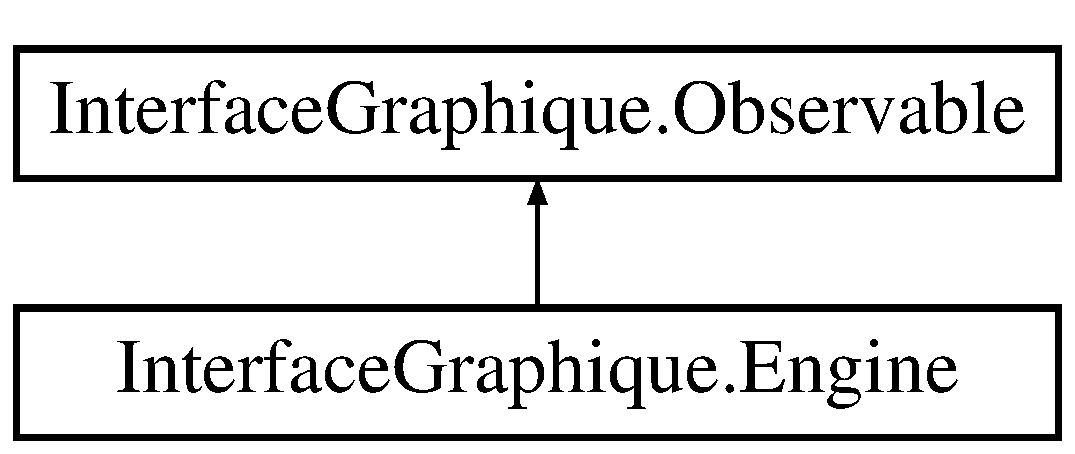
\includegraphics[height=2.000000cm]{class_interface_graphique_1_1_engine}
\end{center}
\end{figure}
\subsection*{Fonctions membres publiques}
\begin{DoxyCompactItemize}
\item 
\hypertarget{class_interface_graphique_1_1_engine_a8c04978eccf024796983289289203f82}{void {\bfseries subscribe} (\hyperlink{interface_interface_graphique_1_1_observer}{Observer} o)}\label{class_interface_graphique_1_1_engine_a8c04978eccf024796983289289203f82}

\item 
\hypertarget{class_interface_graphique_1_1_engine_a895121412380b33a67828f1068219a89}{void {\bfseries unsubscribe} (\hyperlink{interface_interface_graphique_1_1_observer}{Observer} o)}\label{class_interface_graphique_1_1_engine_a895121412380b33a67828f1068219a89}

\item 
\hypertarget{class_interface_graphique_1_1_engine_a6909b848f3b91e4bb7b8c0b5e333c2de}{void {\bfseries zoomer\-In} ()}\label{class_interface_graphique_1_1_engine_a6909b848f3b91e4bb7b8c0b5e333c2de}

\item 
\hypertarget{class_interface_graphique_1_1_engine_ab957792fa2360ef7c4f5f04e10c6d74a}{void {\bfseries zoomer\-Out} ()}\label{class_interface_graphique_1_1_engine_ab957792fa2360ef7c4f5f04e10c6d74a}

\item 
\hypertarget{class_interface_graphique_1_1_engine_a0fb07b6bff1c88bdfe1e2b5adcb34cf1}{void {\bfseries save} (string file\-Path)}\label{class_interface_graphique_1_1_engine_a0fb07b6bff1c88bdfe1e2b5adcb34cf1}

\item 
\hypertarget{class_interface_graphique_1_1_engine_a94b583a2122b3dc2f6e0567b80b4ca50}{void {\bfseries load} (string file\-Path)}\label{class_interface_graphique_1_1_engine_a94b583a2122b3dc2f6e0567b80b4ca50}

\item 
\hypertarget{class_interface_graphique_1_1_engine_a0a39b1977a086a14c6e234fedbf442d3}{void {\bfseries reset\-Map} ()}\label{class_interface_graphique_1_1_engine_a0a39b1977a086a14c6e234fedbf442d3}

\item 
\hypertarget{class_interface_graphique_1_1_engine_af89449879c6caf46a2f8c499558b5426}{void {\bfseries set\-Selected\-Node\-Data} (\hyperlink{struct_interface_graphique_1_1_node_data}{Node\-Data} data)}\label{class_interface_graphique_1_1_engine_af89449879c6caf46a2f8c499558b5426}

\item 
\hypertarget{class_interface_graphique_1_1_engine_aa46f12913f60c43e4e41822a4ff2878e}{void {\bfseries add\-Node} (string type)}\label{class_interface_graphique_1_1_engine_aa46f12913f60c43e4e41822a4ff2878e}

\item 
\hypertarget{class_interface_graphique_1_1_engine_a2da939e4abf78842a17cb2233484be76}{void {\bfseries delete\-Obj} ()}\label{class_interface_graphique_1_1_engine_a2da939e4abf78842a17cb2233484be76}

\item 
\hypertarget{class_interface_graphique_1_1_engine_a7c87261c9f2478f881a4a52c6cb86445}{bool {\bfseries is\-Mouse\-On\-Table} ()}\label{class_interface_graphique_1_1_engine_a7c87261c9f2478f881a4a52c6cb86445}

\item 
\hypertarget{class_interface_graphique_1_1_engine_a3ce229a326130eaad8094a871c8293f5}{bool {\bfseries update\-Node} ()}\label{class_interface_graphique_1_1_engine_a3ce229a326130eaad8094a871c8293f5}

\item 
\hypertarget{class_interface_graphique_1_1_engine_ac54d12909eaa18c9291320f2543de5f4}{void {\bfseries duplicate} ()}\label{class_interface_graphique_1_1_engine_ac54d12909eaa18c9291320f2543de5f4}

\item 
\hypertarget{class_interface_graphique_1_1_engine_a5675cbf578d78cb4cfd792bfa5d3b0b8}{void {\bfseries set\-Init\-Pos} ()}\label{class_interface_graphique_1_1_engine_a5675cbf578d78cb4cfd792bfa5d3b0b8}

\item 
\hypertarget{class_interface_graphique_1_1_engine_a0eab161c6a7ea2c8b1ff0de5fc0a6385}{void {\bfseries check\-Valid\-Pos} ()}\label{class_interface_graphique_1_1_engine_a0eab161c6a7ea2c8b1ff0de5fc0a6385}

\item 
\hypertarget{class_interface_graphique_1_1_engine_ae0376cf6810633d7de94991db45a520d}{void {\bfseries deplacer\-X\-Y} (double deplacement\-X, double deplacement\-Y)}\label{class_interface_graphique_1_1_engine_ae0376cf6810633d7de94991db45a520d}

\item 
\hypertarget{class_interface_graphique_1_1_engine_a25dd642bd70ac8bd97be182e319202bd}{void {\bfseries preparer\-Rectangle\-Elastique} ()}\label{class_interface_graphique_1_1_engine_a25dd642bd70ac8bd97be182e319202bd}

\item 
\hypertarget{class_interface_graphique_1_1_engine_ae2ac0bc1759b93bf2ed6f8c9e0b3169b}{void {\bfseries initialiser\-Rectangle\-Elastique} ()}\label{class_interface_graphique_1_1_engine_ae2ac0bc1759b93bf2ed6f8c9e0b3169b}

\item 
\hypertarget{class_interface_graphique_1_1_engine_a9ef94abf1484db36727cce8a4d22ef49}{void {\bfseries mettre\-A\-Jour\-Rectangle\-Elastique} ()}\label{class_interface_graphique_1_1_engine_a9ef94abf1484db36727cce8a4d22ef49}

\item 
\hypertarget{class_interface_graphique_1_1_engine_a92fab836460aa2e6ec4ec009bdcd2a2f}{void {\bfseries terminer\-Rectangle\-Elastique} ()}\label{class_interface_graphique_1_1_engine_a92fab836460aa2e6ec4ec009bdcd2a2f}

\item 
\hypertarget{class_interface_graphique_1_1_engine_a5da401843c64cfbf6442664454a64f57}{void {\bfseries afficher\-Fantome} ()}\label{class_interface_graphique_1_1_engine_a5da401843c64cfbf6442664454a64f57}

\item 
\hypertarget{class_interface_graphique_1_1_engine_afeffcb9f37cc862e34f558324948cd41}{bool {\bfseries abort\-Composite\-Node} ()}\label{class_interface_graphique_1_1_engine_afeffcb9f37cc862e34f558324948cd41}

\item 
\hypertarget{class_interface_graphique_1_1_engine_a9e974b7c21360ba5869449a921b1fb04}{bool {\bfseries abort\-Terminal\-Node} ()}\label{class_interface_graphique_1_1_engine_a9e974b7c21360ba5869449a921b1fb04}

\item 
\hypertarget{class_interface_graphique_1_1_engine_a14d27e1edfc6f00d9007959cf70b91e6}{void {\bfseries initialize\-Duplication} ()}\label{class_interface_graphique_1_1_engine_a14d27e1edfc6f00d9007959cf70b91e6}

\item 
\hypertarget{class_interface_graphique_1_1_engine_ae511ccb9dd9a6b8f2c76296824774a17}{bool {\bfseries update\-Duplication} ()}\label{class_interface_graphique_1_1_engine_ae511ccb9dd9a6b8f2c76296824774a17}

\item 
\hypertarget{class_interface_graphique_1_1_engine_a8c1b430ab3eac66594cb5ebb8e4efd4a}{bool {\bfseries end\-Duplication} ()}\label{class_interface_graphique_1_1_engine_a8c1b430ab3eac66594cb5ebb8e4efd4a}

\item 
\hypertarget{class_interface_graphique_1_1_engine_a7383d6a2834b761bf0e311fdbf460d24}{void {\bfseries translate} (float delta\-X, float delta\-Y, float delta\-Z)}\label{class_interface_graphique_1_1_engine_a7383d6a2834b761bf0e311fdbf460d24}

\item 
\hypertarget{class_interface_graphique_1_1_engine_a13f9dce829254dbc31fe01aadd1ba8c6}{void {\bfseries rotate} (float delta\-X, float delta\-Y, float delta\-Z)}\label{class_interface_graphique_1_1_engine_a13f9dce829254dbc31fe01aadd1ba8c6}

\item 
\hypertarget{class_interface_graphique_1_1_engine_aed36e2c31333883918d7103305b96236}{void {\bfseries set\-Init\-Angle} ()}\label{class_interface_graphique_1_1_engine_aed36e2c31333883918d7103305b96236}

\item 
\hypertarget{class_interface_graphique_1_1_engine_a0129ba7f711fbf300f354611a8febfd1}{void {\bfseries scale} (float delta\-X, float delta\-Y, float delta\-Z)}\label{class_interface_graphique_1_1_engine_a0129ba7f711fbf300f354611a8febfd1}

\item 
\hypertarget{class_interface_graphique_1_1_engine_a2dab2445d57cc6cfd90f75e613360614}{void {\bfseries set\-Init\-Scale} ()}\label{class_interface_graphique_1_1_engine_a2dab2445d57cc6cfd90f75e613360614}

\item 
\hypertarget{class_interface_graphique_1_1_engine_a2e7f0b1331fd2ee58915a022ec3d579d}{void {\bfseries select\-All} ()}\label{class_interface_graphique_1_1_engine_a2e7f0b1331fd2ee58915a022ec3d579d}

\item 
\hypertarget{class_interface_graphique_1_1_engine_a18cc8cefa5e5a0544d71b80e3c5d8335}{void {\bfseries select\-Object} (bool keep\-Others)}\label{class_interface_graphique_1_1_engine_a18cc8cefa5e5a0544d71b80e3c5d8335}

\item 
\hypertarget{class_interface_graphique_1_1_engine_a8bd0f5e2f7e3549600ba8b5197c344cc}{void {\bfseries select\-Multiple\-Objects} (bool keep\-Others)}\label{class_interface_graphique_1_1_engine_a8bd0f5e2f7e3549600ba8b5197c344cc}

\item 
\hypertarget{class_interface_graphique_1_1_engine_a27a5122603c015861fa75a756c564805}{int {\bfseries get\-Nb\-Nodes\-Selected} ()}\label{class_interface_graphique_1_1_engine_a27a5122603c015861fa75a756c564805}

\item 
\hypertarget{class_interface_graphique_1_1_engine_a57721ea5517a67c6f051120eb0807c9b}{void {\bfseries set\-View\-Init} ()}\label{class_interface_graphique_1_1_engine_a57721ea5517a67c6f051120eb0807c9b}

\item 
\hypertarget{class_interface_graphique_1_1_engine_a541c191ef2d8df168d7a39afbaa57886}{void {\bfseries move\-Camera\-Mouse} ()}\label{class_interface_graphique_1_1_engine_a541c191ef2d8df168d7a39afbaa57886}

\item 
\hypertarget{class_interface_graphique_1_1_engine_a45950feca3f12fb017f561672375a9ac}{void {\bfseries zoom\-Out\-Rectangle} ()}\label{class_interface_graphique_1_1_engine_a45950feca3f12fb017f561672375a9ac}

\item 
\hypertarget{class_interface_graphique_1_1_engine_ad7cdab0d23d83bdb1b1cdf65ca81db44}{void {\bfseries zoom\-In\-Rectangle} ()}\label{class_interface_graphique_1_1_engine_ad7cdab0d23d83bdb1b1cdf65ca81db44}

\item 
\hypertarget{class_interface_graphique_1_1_engine_ac41c680c622de10310d537685176f928}{void {\bfseries initialiser\-Open\-G\-L} (Int\-Ptr handle)}\label{class_interface_graphique_1_1_engine_ac41c680c622de10310d537685176f928}

\item 
\hypertarget{class_interface_graphique_1_1_engine_aa2c408b58d67781eb20456af83618bc6}{void {\bfseries liberer\-Open\-G\-L} ()}\label{class_interface_graphique_1_1_engine_aa2c408b58d67781eb20456af83618bc6}

\item 
\hypertarget{class_interface_graphique_1_1_engine_a410386c23afb65df2439abe7ec22849e}{void {\bfseries dessiner\-Open\-G\-L} ()}\label{class_interface_graphique_1_1_engine_a410386c23afb65df2439abe7ec22849e}

\item 
\hypertarget{class_interface_graphique_1_1_engine_a019dcdf567b73bd2175626c488e55ef9}{void {\bfseries animer} (double temps)}\label{class_interface_graphique_1_1_engine_a019dcdf567b73bd2175626c488e55ef9}

\item 
\hypertarget{class_interface_graphique_1_1_engine_af07a43b62c37b3eb2809c0ceb168990e}{void {\bfseries redimensionner\-Fenetre} (int largeur, int hauteur)}\label{class_interface_graphique_1_1_engine_af07a43b62c37b3eb2809c0ceb168990e}

\item 
\hypertarget{class_interface_graphique_1_1_engine_afe9602521fab45f012520e04d699027a}{void {\bfseries get\-Selected\-Node\-Data} (out \hyperlink{struct_interface_graphique_1_1_node_data}{Node\-Data} data\-Ref)}\label{class_interface_graphique_1_1_engine_afe9602521fab45f012520e04d699027a}

\item 
\hypertarget{class_interface_graphique_1_1_engine_ab1144c7ab4d8e63d6ac181ffdedbf48b}{void {\bfseries start\-Simulation} ()}\label{class_interface_graphique_1_1_engine_ab1144c7ab4d8e63d6ac181ffdedbf48b}

\item 
\hypertarget{class_interface_graphique_1_1_engine_a2ccea8015b159cc18049be76f685821f}{void {\bfseries stop\-Simulation} ()}\label{class_interface_graphique_1_1_engine_a2ccea8015b159cc18049be76f685821f}

\item 
\hypertarget{class_interface_graphique_1_1_engine_a74c673351fcb3ae4374fd6de34d54e9c}{void {\bfseries pause\-Simulation} ()}\label{class_interface_graphique_1_1_engine_a74c673351fcb3ae4374fd6de34d54e9c}

\item 
\hypertarget{class_interface_graphique_1_1_engine_a2c17f632c3fcb5b668f6fb11fe45c96d}{void {\bfseries unpause\-Simulation} ()}\label{class_interface_graphique_1_1_engine_a2c17f632c3fcb5b668f6fb11fe45c96d}

\item 
\hypertarget{class_interface_graphique_1_1_engine_abc2be05df3433be5a5f7ca46062b67b7}{void {\bfseries set\-Profile\-Data} (\hyperlink{struct_interface_graphique_1_1_profile_data}{Profile\-Data} data)}\label{class_interface_graphique_1_1_engine_abc2be05df3433be5a5f7ca46062b67b7}

\item 
\hypertarget{class_interface_graphique_1_1_engine_aada00c468796a5a58cb16a7c9531f0c1}{void {\bfseries set\-Debug} (\hyperlink{struct_interface_graphique_1_1_debug_settings}{Debug\-Settings} data)}\label{class_interface_graphique_1_1_engine_aada00c468796a5a58cb16a7c9531f0c1}

\item 
\hypertarget{class_interface_graphique_1_1_engine_a5bf239745398bb639ec1a4442acba65d}{void {\bfseries robot\-Forward} ()}\label{class_interface_graphique_1_1_engine_a5bf239745398bb639ec1a4442acba65d}

\item 
\hypertarget{class_interface_graphique_1_1_engine_a59cbfcd2f7444faf28f010a791ab28fd}{void {\bfseries robot\-Reverse} ()}\label{class_interface_graphique_1_1_engine_a59cbfcd2f7444faf28f010a791ab28fd}

\item 
\hypertarget{class_interface_graphique_1_1_engine_a8cdac374ca861f54ebb70a58da85423d}{void {\bfseries robot\-Turn\-Left} ()}\label{class_interface_graphique_1_1_engine_a8cdac374ca861f54ebb70a58da85423d}

\item 
\hypertarget{class_interface_graphique_1_1_engine_a237f55d615628251be75528c09a6276c}{void {\bfseries robot\-Turn\-Right} ()}\label{class_interface_graphique_1_1_engine_a237f55d615628251be75528c09a6276c}

\item 
\hypertarget{class_interface_graphique_1_1_engine_aa028ac9b0a8b0f0b869a3065d22e9488}{void {\bfseries robot\-Toggle\-Manual\-Control} ()}\label{class_interface_graphique_1_1_engine_aa028ac9b0a8b0f0b869a3065d22e9488}

\end{DoxyCompactItemize}
\subsection*{Attributs protégés}
\begin{DoxyCompactItemize}
\item 
\hypertarget{class_interface_graphique_1_1_engine_a637816e50122a2ce73b5b16e0cc6909f}{List$<$ \hyperlink{interface_interface_graphique_1_1_observer}{Observer} $>$ {\bfseries observers}}\label{class_interface_graphique_1_1_engine_a637816e50122a2ce73b5b16e0cc6909f}

\end{DoxyCompactItemize}


La documentation de cette classe a été générée à partir du fichier suivant \-:\begin{DoxyCompactItemize}
\item 
C\-:/\-Users/saron/\-Documents/inf2990-\/01/\-Sources/\-Interface\-Graphique/Engine.\-cs\end{DoxyCompactItemize}

\hypertarget{class_etat_open_g_l}{}\section{Etat\+Open\+G\+L Class Reference}
\label{class_etat_open_g_l}\index{Etat\+Open\+G\+L@{Etat\+Open\+G\+L}}


Classe qui représente l\textquotesingle{}état des variables de la machine Open\+G\+L.  




{\ttfamily \#include $<$Etat\+Open\+G\+L.\+h$>$}

\subsection*{Public Member Functions}
\begin{DoxyCompactItemize}
\item 
\hyperlink{group__utilitaire_gaf682f61929f2502b08b6b88de07349b6}{Etat\+Open\+G\+L} ()
\begin{DoxyCompactList}\small\item\em Constructeur par défaut. \end{DoxyCompactList}\item 
std\+::string \hyperlink{group__utilitaire_ga13c8aaca9f02431b47b83e36b18f8067}{obtenir\+Chaine\+Gl\+Accum\+Alpha\+Bits} () const 
\begin{DoxyCompactList}\small\item\em Retourne une chaîne représentant l\textquotesingle{}attribut G\+L\+\_\+\+A\+C\+C\+U\+M\+\_\+\+A\+L\+P\+H\+A\+\_\+\+B\+I\+T\+S. \end{DoxyCompactList}\item 
std\+::string \hyperlink{group__utilitaire_ga695387ee2d838c97214c70219d52da10}{obtenir\+Chaine\+Gl\+Accum\+Blue\+Bits} () const 
\begin{DoxyCompactList}\small\item\em Retourne une chaîne représentant l\textquotesingle{}attribut G\+L\+\_\+\+A\+C\+C\+U\+M\+\_\+\+B\+L\+U\+E\+\_\+\+B\+I\+T\+S. \end{DoxyCompactList}\item 
std\+::string \hyperlink{group__utilitaire_gaf3e85f5f434e93aa09376200f3c837ae}{obtenir\+Chaine\+Gl\+Accum\+Clear\+Value} () const 
\begin{DoxyCompactList}\small\item\em Retourne une chaîne représentant l\textquotesingle{}attribut G\+L\+\_\+\+A\+C\+C\+U\+M\+\_\+\+C\+L\+E\+A\+R\+\_\+\+V\+A\+L\+U\+E. \end{DoxyCompactList}\item 
std\+::string \hyperlink{group__utilitaire_gae677b60d2113b1843ba4d2c92fe34c34}{obtenir\+Chaine\+Gl\+Accum\+Green\+Bits} () const 
\begin{DoxyCompactList}\small\item\em Retourne une chaîne représentant l\textquotesingle{}attribut G\+L\+\_\+\+A\+C\+C\+U\+M\+\_\+\+G\+R\+E\+E\+N\+\_\+\+B\+I\+T\+S. \end{DoxyCompactList}\item 
std\+::string \hyperlink{group__utilitaire_ga3405a98de14c30d7a57d954d298b6376}{obtenir\+Chaine\+Gl\+Accum\+Red\+Bits} () const 
\begin{DoxyCompactList}\small\item\em Retourne une chaîne représentant l\textquotesingle{}attribut G\+L\+\_\+\+A\+C\+C\+U\+M\+\_\+\+R\+E\+D\+\_\+\+B\+I\+T\+S. \end{DoxyCompactList}\item 
std\+::string \hyperlink{group__utilitaire_gaf54d9525863334d2d2fd362c7043a4be}{obtenir\+Chaine\+Gl\+Alpha\+Bias} () const 
\begin{DoxyCompactList}\small\item\em Retourne une chaîne représentant l\textquotesingle{}attribut G\+L\+\_\+\+A\+L\+P\+H\+A\+\_\+\+B\+I\+A\+S. \end{DoxyCompactList}\item 
std\+::string \hyperlink{group__utilitaire_ga7ea311e8cfd6aee3cb19e2041b2ba132}{obtenir\+Chaine\+Gl\+Alpha\+Bits} () const 
\begin{DoxyCompactList}\small\item\em Retourne une chaîne représentant l\textquotesingle{}attribut G\+L\+\_\+\+A\+L\+P\+H\+A\+\_\+\+B\+I\+T\+S. \end{DoxyCompactList}\item 
std\+::string \hyperlink{group__utilitaire_ga3b85b93cd7e5d1f12a225f28ece00696}{obtenir\+Chaine\+Gl\+Alpha\+Scale} () const 
\begin{DoxyCompactList}\small\item\em Retourne une chaîne représentant l\textquotesingle{}attribut G\+L\+\_\+\+A\+L\+P\+H\+A\+\_\+\+S\+C\+A\+L\+E. \end{DoxyCompactList}\item 
std\+::string \hyperlink{group__utilitaire_ga9fd2e2270997cf027e38f6a7b8d621a8}{obtenir\+Chaine\+Gl\+Alpha\+Test} () const 
\begin{DoxyCompactList}\small\item\em Retourne une chaîne représentant l\textquotesingle{}attribut G\+L\+\_\+\+A\+L\+P\+H\+A\+\_\+\+T\+E\+S\+T. \end{DoxyCompactList}\item 
std\+::string \hyperlink{group__utilitaire_ga5002fd87fb9aede24afc4c4bb2a61fb1}{obtenir\+Chaine\+Gl\+Alpha\+Test\+Func} () const 
\begin{DoxyCompactList}\small\item\em Retourne une chaîne représentant l\textquotesingle{}attribut G\+L\+\_\+\+A\+L\+P\+H\+A\+\_\+\+T\+E\+S\+T\+\_\+\+F\+U\+N\+C. \end{DoxyCompactList}\item 
std\+::string \hyperlink{group__utilitaire_gacc2904dcf7edec91f24e5e6ea58a780c}{obtenir\+Chaine\+Gl\+Alpha\+Test\+Ref} () const 
\begin{DoxyCompactList}\small\item\em Retourne une chaîne représentant l\textquotesingle{}attribut G\+L\+\_\+\+A\+L\+P\+H\+A\+\_\+\+T\+E\+S\+T\+\_\+\+R\+E\+F. \end{DoxyCompactList}\item 
std\+::string \hyperlink{group__utilitaire_ga59c1e206aa477f625b5499cf328f695b}{obtenir\+Chaine\+Gl\+Attrib\+Stack\+Depth} () const 
\begin{DoxyCompactList}\small\item\em Retourne une chaîne représentant l\textquotesingle{}attribut G\+L\+\_\+\+A\+T\+T\+R\+I\+B\+\_\+\+S\+T\+A\+C\+K\+\_\+\+D\+E\+P\+T\+H. \end{DoxyCompactList}\item 
std\+::string \hyperlink{group__utilitaire_gaaf8d3f8a4dd51812950c32268c8f77c5}{obtenir\+Chaine\+Gl\+Auto\+Normal} () const 
\begin{DoxyCompactList}\small\item\em Retourne une chaîne représentant l\textquotesingle{}attribut G\+L\+\_\+\+A\+U\+T\+O\+\_\+\+N\+O\+R\+M\+A\+L. \end{DoxyCompactList}\item 
std\+::string \hyperlink{group__utilitaire_gab8c780e176faece6cbaa11084e957e8d}{obtenir\+Chaine\+Gl\+Aux\+Buffers} () const 
\begin{DoxyCompactList}\small\item\em Retourne une chaîne représentant l\textquotesingle{}attribut G\+L\+\_\+\+A\+U\+X\+\_\+\+B\+U\+F\+F\+E\+R\+S. \end{DoxyCompactList}\item 
std\+::string \hyperlink{group__utilitaire_ga8a5f949f2b7a9a911c0677d639bebae5}{obtenir\+Chaine\+Gl\+Blend} () const 
\begin{DoxyCompactList}\small\item\em Retourne une chaîne représentant l\textquotesingle{}attribut G\+L\+\_\+\+B\+L\+E\+N\+D. \end{DoxyCompactList}\item 
std\+::string \hyperlink{group__utilitaire_gaa52ab39bcb62d4f8777afddfca458650}{obtenir\+Chaine\+Gl\+Blend\+Dst} () const 
\begin{DoxyCompactList}\small\item\em Retourne une chaîne représentant l\textquotesingle{}attribut G\+L\+\_\+\+B\+L\+E\+N\+D\+\_\+\+D\+S\+T. \end{DoxyCompactList}\item 
std\+::string \hyperlink{group__utilitaire_ga510a36fe5d3e313756e40b5c67b516ba}{obtenir\+Chaine\+Gl\+Blend\+Src} () const 
\begin{DoxyCompactList}\small\item\em Retourne une chaîne représentant l\textquotesingle{}attribut G\+L\+\_\+\+B\+L\+E\+N\+D\+\_\+\+S\+R\+C. \end{DoxyCompactList}\item 
std\+::string \hyperlink{group__utilitaire_ga95f9a6baabd65a0cdd4b1e5cbeb4f678}{obtenir\+Chaine\+Gl\+Blue\+Bias} () const 
\begin{DoxyCompactList}\small\item\em Retourne une chaîne représentant l\textquotesingle{}attribut G\+L\+\_\+\+B\+L\+U\+E\+\_\+\+B\+I\+A\+S. \end{DoxyCompactList}\item 
std\+::string \hyperlink{group__utilitaire_ga125172f1c5c4ef27c20c4e52a70ce38a}{obtenir\+Chaine\+Gl\+Blue\+Bits} () const 
\begin{DoxyCompactList}\small\item\em Retourne une chaîne représentant l\textquotesingle{}attribut G\+L\+\_\+\+B\+L\+U\+E\+\_\+\+B\+I\+T\+S. \end{DoxyCompactList}\item 
std\+::string \hyperlink{group__utilitaire_ga8422f585aba4fc07dcaac22e6cf587b3}{obtenir\+Chaine\+Gl\+Blue\+Scale} () const 
\begin{DoxyCompactList}\small\item\em Retourne une chaîne représentant l\textquotesingle{}attribut G\+L\+\_\+\+B\+L\+U\+E\+\_\+\+S\+C\+A\+L\+E. \end{DoxyCompactList}\item 
std\+::string \hyperlink{group__utilitaire_gad57f6d8da9cffeae2204a77e6e5f9292}{obtenir\+Chaine\+Gl\+Client\+Attrib\+Stack\+Depth} () const 
\begin{DoxyCompactList}\small\item\em Retourne une chaîne représentant l\textquotesingle{}attribut G\+L\+\_\+\+C\+L\+I\+E\+N\+T\+\_\+\+A\+T\+T\+R\+I\+B\+\_\+\+S\+T\+A\+C\+K\+\_\+\+D\+E\+P\+T\+H. \end{DoxyCompactList}\item 
std\+::string \hyperlink{group__utilitaire_ga7deb847efbc619585d5e8c9f6600204c}{obtenir\+Chaine\+Gl\+Clip\+Planei} () const 
\begin{DoxyCompactList}\small\item\em Retourne une chaîne représentant l\textquotesingle{}attribut G\+L\+\_\+\+C\+L\+I\+P\+\_\+\+P\+L\+A\+N\+Ei. \end{DoxyCompactList}\item 
std\+::string \hyperlink{group__utilitaire_ga8fae4f702f9be3574209f0721b6768ba}{obtenir\+Chaine\+Gl\+Color\+Array} () const 
\begin{DoxyCompactList}\small\item\em Retourne une chaîne représentant l\textquotesingle{}attribut G\+L\+\_\+\+C\+O\+L\+O\+R\+\_\+\+A\+R\+R\+A\+Y. \end{DoxyCompactList}\item 
std\+::string \hyperlink{group__utilitaire_gad1e82d8c71b8e2a76c806e1c92cbb669}{obtenir\+Chaine\+Gl\+Color\+Array\+Size} () const 
\begin{DoxyCompactList}\small\item\em Retourne une chaîne représentant l\textquotesingle{}attribut G\+L\+\_\+\+C\+O\+L\+O\+R\+\_\+\+A\+R\+R\+A\+Y\+\_\+\+S\+I\+Z\+E. \end{DoxyCompactList}\item 
std\+::string \hyperlink{group__utilitaire_gab499d52456b097364de8300cc6af6808}{obtenir\+Chaine\+Gl\+Color\+Array\+Stride} () const 
\begin{DoxyCompactList}\small\item\em Retourne une chaîne représentant l\textquotesingle{}attribut G\+L\+\_\+\+C\+O\+L\+O\+R\+\_\+\+A\+R\+R\+A\+Y\+\_\+\+S\+T\+R\+I\+D\+E. \end{DoxyCompactList}\item 
std\+::string \hyperlink{group__utilitaire_gae77f9acd8bdebe2e7bb39660e03b3e28}{obtenir\+Chaine\+Gl\+Color\+Array\+Type} () const 
\begin{DoxyCompactList}\small\item\em Retourne une chaîne représentant l\textquotesingle{}attribut G\+L\+\_\+\+C\+O\+L\+O\+R\+\_\+\+A\+R\+R\+A\+Y\+\_\+\+T\+Y\+P\+E. \end{DoxyCompactList}\item 
std\+::string \hyperlink{group__utilitaire_ga7de74c129bd5c5038e7f3d03a5508f72}{obtenir\+Chaine\+Gl\+Color\+Clear\+Value} () const 
\begin{DoxyCompactList}\small\item\em Retourne une chaîne représentant l\textquotesingle{}attribut G\+L\+\_\+\+C\+O\+L\+O\+R\+\_\+\+C\+L\+E\+A\+R\+\_\+\+V\+A\+L\+U\+E. \end{DoxyCompactList}\item 
std\+::string \hyperlink{group__utilitaire_gac48e5f8e10bfcd96670a537164a0a8ff}{obtenir\+Chaine\+Gl\+Color\+Logic\+Op} () const 
\begin{DoxyCompactList}\small\item\em Retourne une chaîne représentant l\textquotesingle{}attribut G\+L\+\_\+\+C\+O\+L\+O\+R\+\_\+\+L\+O\+G\+I\+C\+\_\+\+O\+P. \end{DoxyCompactList}\item 
std\+::string \hyperlink{group__utilitaire_gae53c823bf9d4e4305baf00f4d7da96af}{obtenir\+Chaine\+Gl\+Color\+Material} () const 
\begin{DoxyCompactList}\small\item\em Retourne une chaîne représentant l\textquotesingle{}attribut G\+L\+\_\+\+C\+O\+L\+O\+R\+\_\+\+M\+A\+T\+E\+R\+I\+A\+L. \end{DoxyCompactList}\item 
std\+::string \hyperlink{group__utilitaire_gaec66f0ae860a11d50b0e1cf2def483bf}{obtenir\+Chaine\+Gl\+Color\+Material\+Face} () const 
\begin{DoxyCompactList}\small\item\em Retourne une chaîne représentant l\textquotesingle{}attribut G\+L\+\_\+\+C\+O\+L\+O\+R\+\_\+\+M\+A\+T\+E\+R\+I\+A\+L\+\_\+\+F\+A\+C\+E. \end{DoxyCompactList}\item 
std\+::string \hyperlink{group__utilitaire_gad2b7f4282f94a24c4b5129854732c36a}{obtenir\+Chaine\+Gl\+Color\+Material\+Parameter} () const 
\begin{DoxyCompactList}\small\item\em Retourne une chaîne représentant l\textquotesingle{}attribut G\+L\+\_\+\+C\+O\+L\+O\+R\+\_\+\+M\+A\+T\+E\+R\+I\+A\+L\+\_\+\+P\+A\+R\+A\+M\+E\+T\+E\+R. \end{DoxyCompactList}\item 
\hypertarget{group__utilitaire_ga677eb5add1db0999f73a7c6febefe4d8}{}std\+::string \hyperlink{group__utilitaire_ga677eb5add1db0999f73a7c6febefe4d8}{obtenir\+Chaine\+Gl\+Color\+Writemask} () const \label{group__utilitaire_ga677eb5add1db0999f73a7c6febefe4d8}

\begin{DoxyCompactList}\small\item\em Retourne une chaîne représentant l\textquotesingle{}attribut G\+L\+\_\+\+C\+O\+L\+O\+R\+\_\+\+W\+R\+I\+T\+E\+M\+A\+S\+K. \end{DoxyCompactList}\item 
std\+::string \hyperlink{group__utilitaire_ga6c53044cfb9b67582efe6415ff1f1f49}{obtenir\+Chaine\+Gl\+Cull\+Face} () const 
\begin{DoxyCompactList}\small\item\em Retourne une chaîne représentant l\textquotesingle{}attribut G\+L\+\_\+\+C\+U\+L\+L\+\_\+\+F\+A\+C\+E. \end{DoxyCompactList}\item 
std\+::string \hyperlink{group__utilitaire_ga0601a9f84791de8e9ab33841308ecea0}{obtenir\+Chaine\+Gl\+Cull\+Face\+Mode} () const 
\begin{DoxyCompactList}\small\item\em Retourne une chaîne représentant l\textquotesingle{}attribut G\+L\+\_\+\+C\+U\+L\+L\+\_\+\+F\+A\+C\+E\+\_\+\+M\+O\+D\+E. \end{DoxyCompactList}\item 
std\+::string \hyperlink{group__utilitaire_gabe349174d65850291bc46f7b524dac44}{obtenir\+Chaine\+Gl\+Current\+Color} () const 
\begin{DoxyCompactList}\small\item\em Retourne une chaîne représentant l\textquotesingle{}attribut G\+L\+\_\+\+C\+U\+R\+R\+E\+N\+T\+\_\+\+C\+O\+L\+O\+R. \end{DoxyCompactList}\item 
std\+::string \hyperlink{group__utilitaire_ga222790a07e4a9cacfbe2f68cd97fd8d9}{obtenir\+Chaine\+Gl\+Current\+Index} () const 
\begin{DoxyCompactList}\small\item\em Retourne une chaîne représentant l\textquotesingle{}attribut G\+L\+\_\+\+C\+U\+R\+R\+E\+N\+T\+\_\+\+I\+N\+D\+E\+X. \end{DoxyCompactList}\item 
std\+::string \hyperlink{group__utilitaire_gac6c54789d936998634ad29c80e150d92}{obtenir\+Chaine\+Gl\+Current\+Normal} () const 
\begin{DoxyCompactList}\small\item\em Retourne une chaîne représentant l\textquotesingle{}attribut G\+L\+\_\+\+C\+U\+R\+R\+E\+N\+T\+\_\+\+N\+O\+R\+M\+A\+L. \end{DoxyCompactList}\item 
std\+::string \hyperlink{group__utilitaire_ga62ef22c97a3ecc8c7e956f2fd7267b9d}{obtenir\+Chaine\+Gl\+Current\+Raster\+Color} () const 
\begin{DoxyCompactList}\small\item\em Retourne une chaîne représentant l\textquotesingle{}attribut G\+L\+\_\+\+C\+U\+R\+R\+E\+N\+T\+\_\+\+R\+A\+S\+T\+E\+R\+\_\+\+C\+O\+L\+O\+R. \end{DoxyCompactList}\item 
std\+::string \hyperlink{group__utilitaire_ga130c72bf45a65d7d7770c77c7f71cf5c}{obtenir\+Chaine\+Gl\+Current\+Raster\+Distance} () const 
\begin{DoxyCompactList}\small\item\em Retourne une chaîne représentant l\textquotesingle{}attribut G\+L\+\_\+\+C\+U\+R\+R\+E\+N\+T\+\_\+\+R\+A\+S\+T\+E\+R\+\_\+\+D\+I\+S\+T\+A\+N\+C\+E. \end{DoxyCompactList}\item 
std\+::string \hyperlink{group__utilitaire_ga9d14728a6f086186ff9ec92738952892}{obtenir\+Chaine\+Gl\+Current\+Raster\+Index} () const 
\begin{DoxyCompactList}\small\item\em Retourne une chaîne représentant l\textquotesingle{}attribut G\+L\+\_\+\+C\+U\+R\+R\+E\+N\+T\+\_\+\+R\+A\+S\+T\+E\+R\+\_\+\+I\+N\+D\+E\+X. \end{DoxyCompactList}\item 
std\+::string \hyperlink{group__utilitaire_ga1151f4eee3a50e14e0157b18b6fefaa4}{obtenir\+Chaine\+Gl\+Current\+Raster\+Position} () const 
\begin{DoxyCompactList}\small\item\em Retourne une chaîne représentant l\textquotesingle{}attribut G\+L\+\_\+\+C\+U\+R\+R\+E\+N\+T\+\_\+\+R\+A\+S\+T\+E\+R\+\_\+\+P\+O\+S\+I\+T\+I\+O\+N. \end{DoxyCompactList}\item 
std\+::string \hyperlink{group__utilitaire_gaa95c762062531085430d3bd8381c1ab1}{obtenir\+Chaine\+Gl\+Current\+Raster\+Position\+Valid} () const 
\begin{DoxyCompactList}\small\item\em Retourne une chaîne représentant l\textquotesingle{}attribut G\+L\+\_\+\+C\+U\+R\+R\+E\+N\+T\+\_\+\+R\+A\+S\+T\+E\+R\+\_\+\+P\+O\+S\+I\+T\+I\+O\+N\+\_\+\+V\+A\+L\+I\+D. \end{DoxyCompactList}\item 
std\+::string \hyperlink{group__utilitaire_gae1b30e504db9237dce13eade239c8c5a}{obtenir\+Chaine\+Gl\+Current\+Raster\+Texture\+Coords} () const 
\begin{DoxyCompactList}\small\item\em Retourne une chaîne représentant l\textquotesingle{}attribut G\+L\+\_\+\+C\+U\+R\+R\+E\+N\+T\+\_\+\+R\+A\+S\+T\+E\+R\+\_\+\+T\+E\+X\+T\+U\+R\+E\+\_\+\+C\+O\+O\+R\+D\+S. \end{DoxyCompactList}\item 
std\+::string \hyperlink{group__utilitaire_ga5bf6abadfe9d63e576d34c94c93ee8f0}{obtenir\+Chaine\+Gl\+Current\+Texture\+Coords} () const 
\begin{DoxyCompactList}\small\item\em Retourne une chaîne représentant l\textquotesingle{}attribut G\+L\+\_\+\+C\+U\+R\+R\+E\+N\+T\+\_\+\+T\+E\+X\+T\+U\+R\+E\+\_\+\+C\+O\+O\+R\+D\+S. \end{DoxyCompactList}\item 
std\+::string \hyperlink{group__utilitaire_gae3e587b7e9f860f3874823a3c4ab7d71}{obtenir\+Chaine\+Gl\+Depth\+Bias} () const 
\begin{DoxyCompactList}\small\item\em Retourne une chaîne représentant l\textquotesingle{}attribut G\+L\+\_\+\+D\+E\+P\+T\+H\+\_\+\+B\+I\+A\+S. \end{DoxyCompactList}\item 
std\+::string \hyperlink{group__utilitaire_gae1dffc44c8e27d7cb249064cfe35653e}{obtenir\+Chaine\+Gl\+Depth\+Bits} () const 
\begin{DoxyCompactList}\small\item\em Retourne une chaîne représentant l\textquotesingle{}attribut G\+L\+\_\+\+D\+E\+P\+T\+H\+\_\+\+B\+I\+T\+S. \end{DoxyCompactList}\item 
std\+::string \hyperlink{group__utilitaire_gad8b3e2701fb07b0178b5015868818509}{obtenir\+Chaine\+Gl\+Depth\+Clear\+Value} () const 
\begin{DoxyCompactList}\small\item\em Retourne une chaîne représentant l\textquotesingle{}attribut G\+L\+\_\+\+D\+E\+P\+T\+H\+\_\+\+C\+L\+E\+A\+R\+\_\+\+V\+A\+L\+U\+E. \end{DoxyCompactList}\item 
std\+::string \hyperlink{group__utilitaire_gac0dff9e4aee8f969fe6e688bb407dcc9}{obtenir\+Chaine\+Gl\+Depth\+Func} () const 
\begin{DoxyCompactList}\small\item\em Retourne une chaîne représentant l\textquotesingle{}attribut G\+L\+\_\+\+D\+E\+P\+T\+H\+\_\+\+F\+U\+N\+C. \end{DoxyCompactList}\item 
std\+::string \hyperlink{group__utilitaire_ga9921b541644f4dc3b64a4ffd4a661a09}{obtenir\+Chaine\+Gl\+Depth\+Range} () const 
\begin{DoxyCompactList}\small\item\em Retourne une chaîne représentant l\textquotesingle{}attribut G\+L\+\_\+\+D\+E\+P\+T\+H\+\_\+\+R\+A\+N\+G\+E. \end{DoxyCompactList}\item 
std\+::string \hyperlink{group__utilitaire_ga4fac162003ef8c012c16ecd9041794ae}{obtenir\+Chaine\+Gl\+Depth\+Scale} () const 
\begin{DoxyCompactList}\small\item\em Retourne une chaîne représentant l\textquotesingle{}attribut G\+L\+\_\+\+D\+E\+P\+T\+H\+\_\+\+S\+C\+A\+L\+E. \end{DoxyCompactList}\item 
std\+::string \hyperlink{group__utilitaire_ga712bcce1fd6c63377d2b3c9c421f7559}{obtenir\+Chaine\+Gl\+Depth\+Test} () const 
\begin{DoxyCompactList}\small\item\em Retourne une chaîne représentant l\textquotesingle{}attribut G\+L\+\_\+\+D\+E\+P\+T\+H\+\_\+\+T\+E\+S\+T. \end{DoxyCompactList}\item 
std\+::string \hyperlink{group__utilitaire_gaec88db9c85bfd66909d3172982025862}{obtenir\+Chaine\+Gl\+Depth\+Writemask} () const 
\begin{DoxyCompactList}\small\item\em Retourne une chaîne représentant l\textquotesingle{}attribut G\+L\+\_\+\+D\+E\+P\+T\+H\+\_\+\+W\+R\+I\+T\+E\+M\+A\+S\+K. \end{DoxyCompactList}\item 
std\+::string \hyperlink{group__utilitaire_gabc6e75dad01908ff21a473d75483f691}{obtenir\+Chaine\+Gl\+Dither} () const 
\begin{DoxyCompactList}\small\item\em Retourne une chaîne représentant l\textquotesingle{}attribut G\+L\+\_\+\+D\+I\+T\+H\+E\+R. \end{DoxyCompactList}\item 
std\+::string \hyperlink{group__utilitaire_gae8239c45bba646389f06a6bdd49670f3}{obtenir\+Chaine\+Gl\+Doublebuffer} () const 
\begin{DoxyCompactList}\small\item\em Retourne une chaîne représentant l\textquotesingle{}attribut G\+L\+\_\+\+D\+O\+U\+B\+L\+E\+B\+U\+F\+F\+E\+R. \end{DoxyCompactList}\item 
std\+::string \hyperlink{group__utilitaire_ga3b705291c7da107645656d5dfb51872a}{obtenir\+Chaine\+Gl\+Draw\+Buffer} () const 
\begin{DoxyCompactList}\small\item\em Retourne une chaîne représentant l\textquotesingle{}attribut G\+L\+\_\+\+D\+R\+A\+W\+\_\+\+B\+U\+F\+F\+E\+R. \end{DoxyCompactList}\item 
std\+::string \hyperlink{group__utilitaire_ga982e0dacd18861db40bc153b8e7748d6}{obtenir\+Chaine\+Gl\+Edge\+Flag} () const 
\begin{DoxyCompactList}\small\item\em Retourne une chaîne représentant l\textquotesingle{}attribut G\+L\+\_\+\+E\+D\+G\+E\+\_\+\+F\+L\+A\+G. \end{DoxyCompactList}\item 
std\+::string \hyperlink{group__utilitaire_gac69166db434f3671eb241b00786be34b}{obtenir\+Chaine\+Gl\+Edge\+Flag\+Array} () const 
\begin{DoxyCompactList}\small\item\em Retourne une chaîne représentant l\textquotesingle{}attribut G\+L\+\_\+\+E\+D\+G\+E\+\_\+\+F\+L\+A\+G\+\_\+\+A\+R\+R\+A\+Y. \end{DoxyCompactList}\item 
std\+::string \hyperlink{group__utilitaire_ga12932637a943b952d6c822af48b4102a}{obtenir\+Chaine\+Gl\+Edge\+Flag\+Array\+Stride} () const 
\begin{DoxyCompactList}\small\item\em Retourne une chaîne représentant l\textquotesingle{}attribut G\+L\+\_\+\+E\+D\+G\+E\+\_\+\+F\+L\+A\+G\+\_\+\+A\+R\+R\+A\+Y\+\_\+\+S\+T\+R\+I\+D\+E. \end{DoxyCompactList}\item 
std\+::string \hyperlink{group__utilitaire_gab0ae8d230f1fe733862032e082cfbd2f}{obtenir\+Chaine\+Gl\+Feedback\+Buffer\+Size} () const 
\begin{DoxyCompactList}\small\item\em Retourne une chaîne représentant l\textquotesingle{}attribut G\+L\+\_\+\+F\+E\+E\+D\+B\+A\+C\+K\+\_\+\+B\+U\+F\+F\+E\+R\+\_\+\+S\+I\+Z\+E. \end{DoxyCompactList}\item 
std\+::string \hyperlink{group__utilitaire_ga30bdbc77ee2c0b27ee48e5de2654d29c}{obtenir\+Chaine\+Gl\+Feedback\+Buffer\+Type} () const 
\begin{DoxyCompactList}\small\item\em Retourne une chaîne représentant l\textquotesingle{}attribut G\+L\+\_\+\+F\+E\+E\+D\+B\+A\+C\+K\+\_\+\+B\+U\+F\+F\+E\+R\+\_\+\+T\+Y\+P\+E. \end{DoxyCompactList}\item 
std\+::string \hyperlink{group__utilitaire_ga73b3d82b8c3940a818e1dab3d69e4899}{obtenir\+Chaine\+Gl\+Fog} () const 
\begin{DoxyCompactList}\small\item\em Retourne une chaîne représentant l\textquotesingle{}attribut G\+L\+\_\+\+F\+O\+G. \end{DoxyCompactList}\item 
std\+::string \hyperlink{group__utilitaire_ga572f199118c8cb77085a7eb21f05f7fb}{obtenir\+Chaine\+Gl\+Fog\+Color} () const 
\begin{DoxyCompactList}\small\item\em Retourne une chaîne représentant l\textquotesingle{}attribut G\+L\+\_\+\+F\+O\+G\+\_\+\+C\+O\+L\+O\+R. \end{DoxyCompactList}\item 
std\+::string \hyperlink{group__utilitaire_ga9ad8c1de41bc053666ffe001bca8f064}{obtenir\+Chaine\+Gl\+Fog\+Density} () const 
\begin{DoxyCompactList}\small\item\em Retourne une chaîne représentant l\textquotesingle{}attribut G\+L\+\_\+\+F\+O\+G\+\_\+\+D\+E\+N\+S\+I\+T\+Y. \end{DoxyCompactList}\item 
std\+::string \hyperlink{group__utilitaire_ga9c6edbc286eed9a47b2e3ed2426e2b92}{obtenir\+Chaine\+Gl\+Fog\+End} () const 
\begin{DoxyCompactList}\small\item\em Retourne une chaîne représentant l\textquotesingle{}attribut G\+L\+\_\+\+F\+O\+G\+\_\+\+E\+N\+D. \end{DoxyCompactList}\item 
std\+::string \hyperlink{group__utilitaire_ga8bd30ecaffe9f7d38e7a447a185dc8d0}{obtenir\+Chaine\+Gl\+Fog\+Hint} () const 
\begin{DoxyCompactList}\small\item\em Retourne une chaîne représentant l\textquotesingle{}attribut G\+L\+\_\+\+F\+O\+G\+\_\+\+H\+I\+N\+T. \end{DoxyCompactList}\item 
std\+::string \hyperlink{group__utilitaire_ga929e0d580e014af6abda36f16fce43c3}{obtenir\+Chaine\+Gl\+Fog\+Index} () const 
\begin{DoxyCompactList}\small\item\em Retourne une chaîne représentant l\textquotesingle{}attribut G\+L\+\_\+\+F\+O\+G\+\_\+\+I\+N\+D\+E\+X. \end{DoxyCompactList}\item 
std\+::string \hyperlink{group__utilitaire_ga1f28b3ec34f9bd4a2080e1252ca64d57}{obtenir\+Chaine\+Gl\+Fog\+Mode} () const 
\begin{DoxyCompactList}\small\item\em Retourne une chaîne représentant l\textquotesingle{}attribut G\+L\+\_\+\+F\+O\+G\+\_\+\+M\+O\+D\+E. \end{DoxyCompactList}\item 
std\+::string \hyperlink{group__utilitaire_ga7063764912254ec440429aee9e8c3f83}{obtenir\+Chaine\+Gl\+Fog\+Start} () const 
\begin{DoxyCompactList}\small\item\em Retourne une chaîne représentant l\textquotesingle{}attribut G\+L\+\_\+\+F\+O\+G\+\_\+\+S\+T\+A\+R\+T. \end{DoxyCompactList}\item 
std\+::string \hyperlink{group__utilitaire_ga5843f630d530a2112407e19b540e3c42}{obtenir\+Chaine\+Gl\+Front\+Face} () const 
\begin{DoxyCompactList}\small\item\em Retourne une chaîne représentant l\textquotesingle{}attribut G\+L\+\_\+\+F\+R\+O\+N\+T\+\_\+\+F\+A\+C\+E. \end{DoxyCompactList}\item 
std\+::string \hyperlink{group__utilitaire_gabb435ce9e5ba38406d8c429a5a0510ed}{obtenir\+Chaine\+Gl\+Green\+Bias} () const 
\begin{DoxyCompactList}\small\item\em Retourne une chaîne représentant l\textquotesingle{}attribut G\+L\+\_\+\+G\+R\+E\+E\+N\+\_\+\+B\+I\+A\+S. \end{DoxyCompactList}\item 
std\+::string \hyperlink{group__utilitaire_ga418e82a0a01a9dfe598780e602b41b2f}{obtenir\+Chaine\+Gl\+Green\+Bits} () const 
\begin{DoxyCompactList}\small\item\em Retourne une chaîne représentant l\textquotesingle{}attribut G\+L\+\_\+\+G\+R\+E\+E\+N\+\_\+\+B\+I\+T\+S. \end{DoxyCompactList}\item 
std\+::string \hyperlink{group__utilitaire_ga933583938ec361ea302f25dd1323b541}{obtenir\+Chaine\+Gl\+Green\+Scale} () const 
\begin{DoxyCompactList}\small\item\em Retourne une chaîne représentant l\textquotesingle{}attribut G\+L\+\_\+\+G\+R\+E\+E\+N\+\_\+\+S\+C\+A\+L\+E. \end{DoxyCompactList}\item 
std\+::string \hyperlink{group__utilitaire_ga63a264a046b4714154de9f26b04ab1f8}{obtenir\+Chaine\+Gl\+Index\+Array} () const 
\begin{DoxyCompactList}\small\item\em Retourne une chaîne représentant l\textquotesingle{}attribut G\+L\+\_\+\+I\+N\+D\+E\+X\+\_\+\+A\+R\+R\+A\+Y. \end{DoxyCompactList}\item 
std\+::string \hyperlink{group__utilitaire_ga79b9f3969a037a0ed02684b41a8a1328}{obtenir\+Chaine\+Gl\+Index\+Array\+Stride} () const 
\begin{DoxyCompactList}\small\item\em Retourne une chaîne représentant l\textquotesingle{}attribut G\+L\+\_\+\+I\+N\+D\+E\+X\+\_\+\+A\+R\+R\+A\+Y\+\_\+\+S\+T\+R\+I\+D\+E. \end{DoxyCompactList}\item 
std\+::string \hyperlink{group__utilitaire_ga8479c06a3ede7442505bb38803be818f}{obtenir\+Chaine\+Gl\+Index\+Array\+Type} () const 
\begin{DoxyCompactList}\small\item\em Retourne une chaîne représentant l\textquotesingle{}attribut G\+L\+\_\+\+I\+N\+D\+E\+X\+\_\+\+A\+R\+R\+A\+Y\+\_\+\+T\+Y\+P\+E. \end{DoxyCompactList}\item 
std\+::string \hyperlink{group__utilitaire_gae88fc4ca05d447c04f08671823a407a3}{obtenir\+Chaine\+Gl\+Index\+Bits} () const 
\begin{DoxyCompactList}\small\item\em Retourne une chaîne représentant l\textquotesingle{}attribut G\+L\+\_\+\+I\+N\+D\+E\+X\+\_\+\+B\+I\+T\+S. \end{DoxyCompactList}\item 
std\+::string \hyperlink{group__utilitaire_gad0d02a72c93d1501432001b500bf6435}{obtenir\+Chaine\+Gl\+Index\+Clear\+Value} () const 
\begin{DoxyCompactList}\small\item\em Retourne une chaîne représentant l\textquotesingle{}attribut G\+L\+\_\+\+I\+N\+D\+E\+X\+\_\+\+C\+L\+E\+A\+R\+\_\+\+V\+A\+L\+U\+E. \end{DoxyCompactList}\item 
std\+::string \hyperlink{group__utilitaire_ga5294ee67327c1a604fe1ac627d539acc}{obtenir\+Chaine\+Gl\+Index\+Logic\+Op} () const 
\begin{DoxyCompactList}\small\item\em Retourne une chaîne représentant l\textquotesingle{}attribut G\+L\+\_\+\+I\+N\+D\+E\+X\+\_\+\+L\+O\+G\+I\+C\+\_\+\+O\+P. \end{DoxyCompactList}\item 
std\+::string \hyperlink{group__utilitaire_ga5413d656a860db0103e85dcd025970e8}{obtenir\+Chaine\+Gl\+Index\+Mode} () const 
\begin{DoxyCompactList}\small\item\em Retourne une chaîne représentant l\textquotesingle{}attribut G\+L\+\_\+\+I\+N\+D\+E\+X\+\_\+\+M\+O\+D\+E. \end{DoxyCompactList}\item 
std\+::string \hyperlink{group__utilitaire_ga2ef77a1752dfc7df305e66d9ebc8fee0}{obtenir\+Chaine\+Gl\+Index\+Offset} () const 
\begin{DoxyCompactList}\small\item\em Retourne une chaîne représentant l\textquotesingle{}attribut G\+L\+\_\+\+I\+N\+D\+E\+X\+\_\+\+O\+F\+F\+S\+E\+T. \end{DoxyCompactList}\item 
std\+::string \hyperlink{group__utilitaire_gabb665544045af095c7c301467b71a53d}{obtenir\+Chaine\+Gl\+Index\+Shift} () const 
\begin{DoxyCompactList}\small\item\em Retourne une chaîne représentant l\textquotesingle{}attribut G\+L\+\_\+\+I\+N\+D\+E\+X\+\_\+\+S\+H\+I\+F\+T. \end{DoxyCompactList}\item 
std\+::string \hyperlink{group__utilitaire_ga7041e09cfd847b59e2fd8b306639b2e2}{obtenir\+Chaine\+Gl\+Index\+Writemask} () const 
\begin{DoxyCompactList}\small\item\em Retourne une chaîne représentant l\textquotesingle{}attribut G\+L\+\_\+\+I\+N\+D\+E\+X\+\_\+\+W\+R\+I\+T\+E\+M\+A\+S\+K. \end{DoxyCompactList}\item 
std\+::string \hyperlink{group__utilitaire_ga373300784f0f42aea9a0d6c78cb01623}{obtenir\+Chaine\+Gl\+Lighti} () const 
\begin{DoxyCompactList}\small\item\em Retourne une chaîne représentant l\textquotesingle{}attribut G\+L\+\_\+\+L\+I\+G\+H\+Ti. \end{DoxyCompactList}\item 
std\+::string \hyperlink{group__utilitaire_gac26fe35af4bad0a50b4890f21e61ea02}{obtenir\+Chaine\+Gl\+Lighting} () const 
\begin{DoxyCompactList}\small\item\em Retourne une chaîne représentant l\textquotesingle{}attribut G\+L\+\_\+\+L\+I\+G\+H\+T\+I\+N\+G. \end{DoxyCompactList}\item 
std\+::string \hyperlink{group__utilitaire_gafee564b101971fe6c901050b13522dc7}{obtenir\+Chaine\+Gl\+Light\+Model\+Ambient} () const 
\begin{DoxyCompactList}\small\item\em Retourne une chaîne représentant l\textquotesingle{}attribut G\+L\+\_\+\+L\+I\+G\+H\+T\+\_\+\+M\+O\+D\+E\+L\+\_\+\+A\+M\+B\+I\+E\+N\+T. \end{DoxyCompactList}\item 
std\+::string \hyperlink{group__utilitaire_gad3dbc66405e9f773549840afceebda51}{obtenir\+Chaine\+Gl\+Light\+Model\+Local\+Viewer} () const 
\begin{DoxyCompactList}\small\item\em Retourne une chaîne représentant l\textquotesingle{}attribut G\+L\+\_\+\+L\+I\+G\+H\+T\+\_\+\+M\+O\+D\+E\+L\+\_\+\+L\+O\+C\+A\+L\+\_\+\+V\+I\+E\+W\+E\+R. \end{DoxyCompactList}\item 
std\+::string \hyperlink{group__utilitaire_gab355049dd400e05dcf9057355f954b2d}{obtenir\+Chaine\+Gl\+Light\+Model\+Two\+Side} () const 
\begin{DoxyCompactList}\small\item\em Retourne une chaîne représentant l\textquotesingle{}attribut G\+L\+\_\+\+L\+I\+G\+H\+T\+\_\+\+M\+O\+D\+E\+L\+\_\+\+T\+W\+O\+\_\+\+S\+I\+D\+E. \end{DoxyCompactList}\item 
std\+::string \hyperlink{group__utilitaire_ga3823c538863f06203e0f72df0af8e517}{obtenir\+Chaine\+Gl\+Line\+Smooth} () const 
\begin{DoxyCompactList}\small\item\em Retourne une chaîne représentant l\textquotesingle{}attribut G\+L\+\_\+\+L\+I\+N\+E\+\_\+\+S\+M\+O\+O\+T\+H. \end{DoxyCompactList}\item 
std\+::string \hyperlink{group__utilitaire_ga259303d6900794169347807035689bc8}{obtenir\+Chaine\+Gl\+Line\+Smooth\+Hint} () const 
\begin{DoxyCompactList}\small\item\em Retourne une chaîne représentant l\textquotesingle{}attribut G\+L\+\_\+\+L\+I\+N\+E\+\_\+\+S\+M\+O\+O\+T\+H\+\_\+\+H\+I\+N\+T. \end{DoxyCompactList}\item 
std\+::string \hyperlink{group__utilitaire_gae6a2fafc56ddcffeb516c7e7451ee620}{obtenir\+Chaine\+Gl\+Line\+Stipple} () const 
\begin{DoxyCompactList}\small\item\em Retourne une chaîne représentant l\textquotesingle{}attribut G\+L\+\_\+\+L\+I\+N\+E\+\_\+\+S\+T\+I\+P\+P\+L\+E. \end{DoxyCompactList}\item 
std\+::string \hyperlink{group__utilitaire_gaf5594a01ce0e3ce08073c9d8adc2dc7d}{obtenir\+Chaine\+Gl\+Line\+Stipple\+Pattern} () const 
\begin{DoxyCompactList}\small\item\em Retourne une chaîne représentant l\textquotesingle{}attribut G\+L\+\_\+\+L\+I\+N\+E\+\_\+\+S\+T\+I\+P\+P\+L\+E\+\_\+\+P\+A\+T\+T\+E\+R\+N. \end{DoxyCompactList}\item 
std\+::string \hyperlink{group__utilitaire_gab9b326741292e41732d5e0b646c4f006}{obtenir\+Chaine\+Gl\+Line\+Stipple\+Repeat} () const 
\begin{DoxyCompactList}\small\item\em Retourne une chaîne représentant l\textquotesingle{}attribut G\+L\+\_\+\+L\+I\+N\+E\+\_\+\+S\+T\+I\+P\+P\+L\+E\+\_\+\+R\+E\+P\+E\+A\+T. \end{DoxyCompactList}\item 
std\+::string \hyperlink{group__utilitaire_gacd329652ea9f177db0c0ad44bc9150bd}{obtenir\+Chaine\+Gl\+Line\+Width} () const 
\begin{DoxyCompactList}\small\item\em Retourne une chaîne représentant l\textquotesingle{}attribut G\+L\+\_\+\+L\+I\+N\+E\+\_\+\+W\+I\+D\+T\+H. \end{DoxyCompactList}\item 
std\+::string \hyperlink{group__utilitaire_ga42e5a43f490a0f90bedf54064921de10}{obtenir\+Chaine\+Gl\+Line\+Width\+Granularity} () const 
\begin{DoxyCompactList}\small\item\em Retourne une chaîne représentant l\textquotesingle{}attribut G\+L\+\_\+\+L\+I\+N\+E\+\_\+\+W\+I\+D\+T\+H\+\_\+\+G\+R\+A\+N\+U\+L\+A\+R\+I\+T\+Y. \end{DoxyCompactList}\item 
std\+::string \hyperlink{group__utilitaire_gacdf3e63f9464f755958fb682f2a45015}{obtenir\+Chaine\+Glline\+Width\+Range} () const 
\begin{DoxyCompactList}\small\item\em Retourne une chaîne représentant l\textquotesingle{}attribut G\+L\+\_\+\+L\+I\+N\+E\+\_\+\+W\+I\+D\+T\+H\+\_\+\+R\+A\+N\+G\+E. \end{DoxyCompactList}\item 
std\+::string \hyperlink{group__utilitaire_ga869ac6c34aaec533fb74b4e8095ae993}{obtenir\+Chaine\+Gl\+List\+Base} () const 
\begin{DoxyCompactList}\small\item\em Retourne une chaîne représentant l\textquotesingle{}attribut G\+L\+\_\+\+L\+I\+S\+T\+\_\+\+B\+A\+S\+E. \end{DoxyCompactList}\item 
std\+::string \hyperlink{group__utilitaire_ga4486b4e688ef8a216e16b7c1a6ec7a61}{obtenir\+Chaine\+Gl\+List\+Index} () const 
\begin{DoxyCompactList}\small\item\em Retourne une chaîne représentant l\textquotesingle{}attribut G\+L\+\_\+\+L\+I\+S\+T\+\_\+\+I\+N\+D\+E\+X. \end{DoxyCompactList}\item 
std\+::string \hyperlink{group__utilitaire_ga75eb73d049c2865922e414f5a06b749a}{obtenir\+Chaine\+Gl\+List\+Mode} () const 
\begin{DoxyCompactList}\small\item\em Retourne une chaîne représentant l\textquotesingle{}attribut G\+L\+\_\+\+L\+I\+S\+T\+\_\+\+M\+O\+D\+E. \end{DoxyCompactList}\item 
std\+::string \hyperlink{group__utilitaire_gaf88292802715427e1a4e58f591b8e67e}{obtenir\+Chaine\+Gl\+Logic\+Op\+Mode} () const 
\begin{DoxyCompactList}\small\item\em Retourne une chaîne représentant l\textquotesingle{}attribut G\+L\+\_\+\+L\+O\+G\+I\+C\+\_\+\+O\+P\+\_\+\+M\+O\+D\+E. \end{DoxyCompactList}\item 
std\+::string \hyperlink{group__utilitaire_gaa3e13a4accbc22c40a52ee9cee9fc3e0}{obtenir\+Chaine\+Gl\+Map1\+Color4} () const 
\begin{DoxyCompactList}\small\item\em Retourne une chaîne représentant l\textquotesingle{}attribut G\+L\+\_\+\+M\+A\+P1\+\_\+\+C\+O\+L\+O\+R\+\_\+4. \end{DoxyCompactList}\item 
std\+::string \hyperlink{group__utilitaire_gad05cd2af4f512deb88aca0b00b0815c4}{obtenir\+Chaine\+Gl\+Map1\+Grid\+Domain} () const 
\begin{DoxyCompactList}\small\item\em Retourne une chaîne représentant l\textquotesingle{}attribut G\+L\+\_\+\+M\+A\+P1\+\_\+\+G\+R\+I\+D\+\_\+\+D\+O\+M\+A\+I\+N. \end{DoxyCompactList}\item 
std\+::string \hyperlink{group__utilitaire_gaef4171a2ed92756d394ed8bae1fc57cd}{obtenir\+Chaine\+Gl\+Map1\+Grid\+Segments} () const 
\begin{DoxyCompactList}\small\item\em Retourne une chaîne représentant l\textquotesingle{}attribut G\+L\+\_\+\+M\+A\+P1\+\_\+\+G\+R\+I\+D\+\_\+\+S\+E\+G\+M\+E\+N\+T\+S. \end{DoxyCompactList}\item 
std\+::string \hyperlink{group__utilitaire_ga52ba9a6fe299e4342d28baac6a83c769}{obtenir\+Chaine\+Gl\+Map1\+Index} () const 
\begin{DoxyCompactList}\small\item\em Retourne une chaîne représentant l\textquotesingle{}attribut G\+L\+\_\+\+M\+A\+P1\+\_\+\+I\+N\+D\+E\+X. \end{DoxyCompactList}\item 
std\+::string \hyperlink{group__utilitaire_gad0e75e07ddc5d51e11b4a9b525ee4190}{obtenir\+Chaine\+Gl\+Map1\+Normal} () const 
\begin{DoxyCompactList}\small\item\em Retourne une chaîne représentant l\textquotesingle{}attribut G\+L\+\_\+\+M\+A\+P1\+\_\+\+N\+O\+R\+M\+A\+L. \end{DoxyCompactList}\item 
std\+::string \hyperlink{group__utilitaire_gaf06cacbe0ee8f4fe4a6f56571fb8c27c}{obtenir\+Chaine\+Gl\+Map1\+Texture\+Coord1} () const 
\begin{DoxyCompactList}\small\item\em Retourne une chaîne représentant l\textquotesingle{}attribut G\+L\+\_\+\+M\+A\+P1\+\_\+\+T\+E\+X\+T\+U\+R\+E\+\_\+\+C\+O\+O\+R\+D\+\_\+1. \end{DoxyCompactList}\item 
std\+::string \hyperlink{group__utilitaire_gade175aafd1123e597959f78fbe04489f}{obtenir\+Chaine\+Gl\+Map1\+Texture\+Coord2} () const 
\begin{DoxyCompactList}\small\item\em Retourne une chaîne représentant l\textquotesingle{}attribut G\+L\+\_\+\+M\+A\+P1\+\_\+\+T\+E\+X\+T\+U\+R\+E\+\_\+\+C\+O\+O\+R\+D\+\_\+2. \end{DoxyCompactList}\item 
std\+::string \hyperlink{group__utilitaire_ga6690ab58fbdae84d2543e29cc9e4c41d}{obtenir\+Chaine\+Gl\+Map1\+Texture\+Coord3} () const 
\begin{DoxyCompactList}\small\item\em Retourne une chaîne représentant l\textquotesingle{}attribut G\+L\+\_\+\+M\+A\+P1\+\_\+\+T\+E\+X\+T\+U\+R\+E\+\_\+\+C\+O\+O\+R\+D\+\_\+3. \end{DoxyCompactList}\item 
std\+::string \hyperlink{group__utilitaire_gab7a65aa462c3a278c42977ed9a35904e}{obtenir\+Chaine\+Gl\+Map1\+Texture\+Coord4} () const 
\begin{DoxyCompactList}\small\item\em Retourne une chaîne représentant l\textquotesingle{}attribut G\+L\+\_\+\+M\+A\+P1\+\_\+\+T\+E\+X\+T\+U\+R\+E\+\_\+\+C\+O\+O\+R\+D\+\_\+4. \end{DoxyCompactList}\item 
std\+::string \hyperlink{group__utilitaire_gafe0e07682a0bb42bb227fecd287de609}{obtenir\+Chaine\+Gl\+Map1\+Vertex3} () const 
\begin{DoxyCompactList}\small\item\em Retourne une chaîne représentant l\textquotesingle{}attribut G\+L\+\_\+\+M\+A\+P1\+\_\+\+V\+E\+R\+T\+E\+X\+\_\+3. \end{DoxyCompactList}\item 
std\+::string \hyperlink{group__utilitaire_gab130a35770d4594bf74a89d18c49697a}{obtenir\+Chaine\+Gl\+Map1\+Vertex4} () const 
\begin{DoxyCompactList}\small\item\em Retourne une chaîne représentant l\textquotesingle{}attribut G\+L\+\_\+\+M\+A\+P1\+\_\+\+V\+E\+R\+T\+E\+X\+\_\+4. \end{DoxyCompactList}\item 
std\+::string \hyperlink{group__utilitaire_ga85dca50f7d25944ca4158173a630d15d}{obtenir\+Chaine\+Gl\+Map2\+Color4} () const 
\begin{DoxyCompactList}\small\item\em Retourne une chaîne représentant l\textquotesingle{}attribut G\+L\+\_\+\+M\+A\+P2\+\_\+\+C\+O\+L\+O\+R\+\_\+4. \end{DoxyCompactList}\item 
std\+::string \hyperlink{group__utilitaire_ga15f308a3995cd63e0bf8ff13fd1024dd}{obtenir\+Chaine\+Gl\+Map2\+Grid\+Domain} () const 
\begin{DoxyCompactList}\small\item\em Retourne une chaîne représentant l\textquotesingle{}attribut G\+L\+\_\+\+M\+A\+P2\+\_\+\+G\+R\+I\+D\+\_\+\+D\+O\+M\+A\+I\+N. \end{DoxyCompactList}\item 
std\+::string \hyperlink{group__utilitaire_ga7cc72b6b6d1f670c6bb2a37bb02f22cc}{obtenir\+Chaine\+Gl\+Map2\+Grid\+Segments} () const 
\begin{DoxyCompactList}\small\item\em Retourne une chaîne représentant l\textquotesingle{}attribut G\+L\+\_\+\+M\+A\+P2\+\_\+\+G\+R\+I\+D\+\_\+\+S\+E\+G\+M\+E\+N\+T\+S. \end{DoxyCompactList}\item 
std\+::string \hyperlink{group__utilitaire_ga5c26c0fce87b7c852f2819ddbc816835}{obtenir\+Chaine\+Gl\+Map2\+Index} () const 
\begin{DoxyCompactList}\small\item\em Retourne une chaîne représentant l\textquotesingle{}attribut G\+L\+\_\+\+M\+A\+P2\+\_\+\+I\+N\+D\+E\+X. \end{DoxyCompactList}\item 
std\+::string \hyperlink{group__utilitaire_ga281e64b376bb0c3f7f7090820a64bd7e}{obtenir\+Chaine\+Gl\+Map2\+Normal} () const 
\begin{DoxyCompactList}\small\item\em Retourne une chaîne représentant l\textquotesingle{}attribut G\+L\+\_\+\+M\+A\+P2\+\_\+\+N\+O\+R\+M\+A\+L. \end{DoxyCompactList}\item 
std\+::string \hyperlink{group__utilitaire_gadb7c67ea193286a4088b9dcc172abef6}{obtenir\+Chaine\+Gl\+Map2\+Texture\+Coord1} () const 
\begin{DoxyCompactList}\small\item\em Retourne une chaîne représentant l\textquotesingle{}attribut G\+L\+\_\+\+M\+A\+P2\+\_\+\+T\+E\+X\+T\+U\+R\+E\+\_\+\+C\+O\+O\+R\+D\+\_\+1. \end{DoxyCompactList}\item 
std\+::string \hyperlink{group__utilitaire_gaf5cb23274f1ad4c504c5aed7947a3432}{obtenir\+Chaine\+Gl\+Map2\+Texture\+Coord2} () const 
\begin{DoxyCompactList}\small\item\em Retourne une chaîne représentant l\textquotesingle{}attribut G\+L\+\_\+\+M\+A\+P2\+\_\+\+T\+E\+X\+T\+U\+R\+E\+\_\+\+C\+O\+O\+R\+D\+\_\+2. \end{DoxyCompactList}\item 
std\+::string \hyperlink{group__utilitaire_gad4b636ae980e2c420c9a7357fe8d58cc}{obtenir\+Chaine\+Gl\+Map2\+Texture\+Coord3} () const 
\begin{DoxyCompactList}\small\item\em Retourne une chaîne représentant l\textquotesingle{}attribut G\+L\+\_\+\+M\+A\+P2\+\_\+\+T\+E\+X\+T\+U\+R\+E\+\_\+\+C\+O\+O\+R\+D\+\_\+3. \end{DoxyCompactList}\item 
std\+::string \hyperlink{group__utilitaire_ga0716a8c85e544f43620ea6664c58b570}{obtenir\+Chaine\+Gl\+Map2\+Texture\+Coord4} () const 
\begin{DoxyCompactList}\small\item\em Retourne une chaîne représentant l\textquotesingle{}attribut G\+L\+\_\+\+M\+A\+P2\+\_\+\+T\+E\+X\+T\+U\+R\+E\+\_\+\+C\+O\+O\+R\+D\+\_\+4. \end{DoxyCompactList}\item 
std\+::string \hyperlink{group__utilitaire_ga7d031ab910660e0f56b3ed4a95d2bfc6}{obtenir\+Chaine\+Gl\+Map2\+Vertex3} () const 
\begin{DoxyCompactList}\small\item\em Retourne une chaîne représentant l\textquotesingle{}attribut G\+L\+\_\+\+M\+A\+P2\+\_\+\+V\+E\+R\+T\+E\+X\+\_\+3. \end{DoxyCompactList}\item 
std\+::string \hyperlink{group__utilitaire_ga866e31b0b0469c11f0c0bee0bb4f9973}{obtenir\+Chaine\+Gl\+Map2\+Vertex4} () const 
\begin{DoxyCompactList}\small\item\em Retourne une chaîne représentant l\textquotesingle{}attribut G\+L\+\_\+\+M\+A\+P2\+\_\+\+V\+E\+R\+T\+E\+X\+\_\+4. \end{DoxyCompactList}\item 
std\+::string \hyperlink{group__utilitaire_ga7224b43655a9b3d8a381bea11d42d401}{obtenir\+Chaine\+Gl\+Map\+Color} () const 
\begin{DoxyCompactList}\small\item\em Retourne une chaîne représentant l\textquotesingle{}attribut G\+L\+\_\+\+M\+A\+P\+\_\+\+C\+O\+L\+O\+R. \end{DoxyCompactList}\item 
std\+::string \hyperlink{group__utilitaire_ga17a6e4887be554b1845d8eb595129b0c}{obtenir\+Chaine\+Gl\+Map\+Stencil} () const 
\begin{DoxyCompactList}\small\item\em Retourne une chaîne représentant l\textquotesingle{}attribut G\+L\+\_\+\+M\+A\+P\+\_\+\+S\+T\+E\+N\+C\+I\+L. \end{DoxyCompactList}\item 
std\+::string \hyperlink{group__utilitaire_ga3cb5f2ef622bebc2786449eda2460d55}{obtenir\+Chaine\+Gl\+Matrix\+Mode} () const 
\begin{DoxyCompactList}\small\item\em Retourne une chaîne représentant l\textquotesingle{}attribut G\+L\+\_\+\+M\+A\+T\+R\+I\+X\+\_\+\+M\+O\+D\+E. \end{DoxyCompactList}\item 
std\+::string \hyperlink{group__utilitaire_ga2085416ccd06cb60bc98ba2207174dd1}{obtenir\+Chaine\+Gl\+Max\+Client\+Attrib\+Stack\+Depth} () const 
\begin{DoxyCompactList}\small\item\em Retourne une chaîne représentant l\textquotesingle{}attribut G\+L\+\_\+\+M\+A\+X\+\_\+\+C\+L\+I\+E\+N\+T\+\_\+\+A\+T\+T\+R\+I\+B\+\_\+\+S\+T\+A\+C\+K\+\_\+\+D\+E\+P\+T\+H. \end{DoxyCompactList}\item 
std\+::string \hyperlink{group__utilitaire_gaa03eca9a37a755a11183714292f89779}{obtenir\+Chaine\+Gl\+Max\+Attrib\+Stack\+Depth} () const 
\begin{DoxyCompactList}\small\item\em Retourne une chaîne représentant l\textquotesingle{}attribut G\+L\+\_\+\+M\+A\+X\+\_\+\+A\+T\+T\+R\+I\+B\+\_\+\+S\+T\+A\+C\+K\+\_\+\+D\+E\+P\+T\+H. \end{DoxyCompactList}\item 
std\+::string \hyperlink{group__utilitaire_gae90d5285df064d711bedd09091ba413b}{obtenir\+Chaine\+Gl\+Max\+Clip\+Planes} () const 
\begin{DoxyCompactList}\small\item\em Retourne une chaîne représentant l\textquotesingle{}attribut G\+L\+\_\+\+M\+A\+X\+\_\+\+C\+L\+I\+P\+\_\+\+P\+L\+A\+N\+E\+S. \end{DoxyCompactList}\item 
std\+::string \hyperlink{group__utilitaire_gaf82e6892182ffe565a05329073a06248}{obtenir\+Chaine\+Gl\+Max\+Eval\+Order} () const 
\begin{DoxyCompactList}\small\item\em Retourne une chaîne représentant l\textquotesingle{}attribut G\+L\+\_\+\+M\+A\+X\+\_\+\+E\+V\+A\+L\+\_\+\+O\+R\+D\+E\+R. \end{DoxyCompactList}\item 
std\+::string \hyperlink{group__utilitaire_ga95b23ba66220abe4def913fd80f31f9c}{obtenir\+Chaine\+Gl\+Max\+Lights} () const 
\begin{DoxyCompactList}\small\item\em Retourne une chaîne représentant l\textquotesingle{}attribut G\+L\+\_\+\+M\+A\+X\+\_\+\+L\+I\+G\+H\+T\+S. \end{DoxyCompactList}\item 
std\+::string \hyperlink{group__utilitaire_gaab626bdfc4cf8d6445955270799c969a}{obtenir\+Chaine\+Gl\+Max\+List\+Nesting} () const 
\begin{DoxyCompactList}\small\item\em Retourne une chaîne représentant l\textquotesingle{}attribut G\+L\+\_\+\+M\+A\+X\+\_\+\+L\+I\+S\+T\+\_\+\+N\+E\+S\+T\+I\+N\+G. \end{DoxyCompactList}\item 
std\+::string \hyperlink{group__utilitaire_ga7a7a64fd525a66dfc542f8d38470e6df}{obtenir\+Chaine\+Gl\+Max\+Modelview\+Stack\+Depth} () const 
\begin{DoxyCompactList}\small\item\em Retourne une chaîne représentant l\textquotesingle{}attribut G\+L\+\_\+\+M\+A\+X\+\_\+\+M\+O\+D\+E\+L\+V\+I\+E\+W\+\_\+\+S\+T\+A\+C\+K\+\_\+\+D\+E\+P\+T\+H. \end{DoxyCompactList}\item 
std\+::string \hyperlink{group__utilitaire_gad22c079b7e29e5cfb6ee2fe9bb220816}{obtenir\+Chaine\+Gl\+Max\+Name\+Stack\+Depth} () const 
\begin{DoxyCompactList}\small\item\em Retourne une chaîne représentant l\textquotesingle{}attribut G\+L\+\_\+\+M\+A\+X\+\_\+\+N\+A\+M\+E\+\_\+\+S\+T\+A\+C\+K\+\_\+\+D\+E\+P\+T\+H. \end{DoxyCompactList}\item 
std\+::string \hyperlink{group__utilitaire_ga266533ff4a35f65c19be95594d07f435}{obtenir\+Chaine\+Gl\+Max\+Pixel\+Map\+Table} () const 
\begin{DoxyCompactList}\small\item\em Retourne une chaîne représentant l\textquotesingle{}attribut G\+L\+\_\+\+M\+A\+X\+\_\+\+P\+I\+X\+E\+L\+\_\+\+M\+A\+P\+\_\+\+T\+A\+B\+L\+E. \end{DoxyCompactList}\item 
std\+::string \hyperlink{group__utilitaire_ga8c2d3530aa09867d9c01d8433839011e}{obtenir\+Chaine\+Gl\+Max\+Projection\+Stack\+Depth} () const 
\begin{DoxyCompactList}\small\item\em Retourne une chaîne représentant l\textquotesingle{}attribut G\+L\+\_\+\+M\+A\+X\+\_\+\+P\+R\+O\+J\+E\+C\+T\+I\+O\+N\+\_\+\+S\+T\+A\+C\+K\+\_\+\+D\+E\+P\+T\+H. \end{DoxyCompactList}\item 
std\+::string \hyperlink{group__utilitaire_gaeba7eaad6682c2c4aa8925501601c606}{obtenir\+Chaine\+Gl\+Max\+Texture\+Size} () const 
\begin{DoxyCompactList}\small\item\em Retourne une chaîne représentant l\textquotesingle{}attribut G\+L\+\_\+\+M\+A\+X\+\_\+\+T\+E\+X\+T\+U\+R\+E\+\_\+\+S\+I\+Z\+E. \end{DoxyCompactList}\item 
std\+::string \hyperlink{group__utilitaire_ga9aac1a0891487831a30125fca75bec93}{obtenir\+Chaine\+Gl\+Max\+Texture\+Stack\+Depth} () const 
\begin{DoxyCompactList}\small\item\em Retourne une chaîne représentant l\textquotesingle{}attribut G\+L\+\_\+\+M\+A\+X\+\_\+\+T\+E\+X\+T\+U\+R\+E\+\_\+\+S\+T\+A\+C\+K\+\_\+\+D\+E\+P\+T\+H. \end{DoxyCompactList}\item 
std\+::string \hyperlink{group__utilitaire_ga0dad12ef08cd32b9fb94e214f00a95a9}{obtenir\+Chaine\+Gl\+Max\+Viewport\+Dims} () const 
\begin{DoxyCompactList}\small\item\em Retourne une chaîne représentant l\textquotesingle{}attribut G\+L\+\_\+\+M\+A\+X\+\_\+\+V\+I\+E\+W\+P\+O\+R\+T\+\_\+\+D\+I\+M\+S. \end{DoxyCompactList}\item 
std\+::string \hyperlink{group__utilitaire_ga44c62c93a914527f821b2aef913fada7}{obtenir\+Chaine\+Gl\+Modelview\+Matrix} () const 
\begin{DoxyCompactList}\small\item\em Retourne une chaîne représentant l\textquotesingle{}attribut G\+L\+\_\+\+M\+O\+D\+E\+L\+V\+I\+E\+W\+\_\+\+M\+A\+T\+R\+I\+X. \end{DoxyCompactList}\item 
std\+::string \hyperlink{group__utilitaire_ga745672a8704edbf33daef5314f9cdfaf}{obtenir\+Chaine\+Gl\+Modelview\+Stack\+Depth} () const 
\begin{DoxyCompactList}\small\item\em Retourne une chaîne représentant l\textquotesingle{}attribut G\+L\+\_\+\+M\+O\+D\+E\+L\+V\+I\+E\+W\+\_\+\+S\+T\+A\+C\+K\+\_\+\+D\+E\+P\+T\+H. \end{DoxyCompactList}\item 
std\+::string \hyperlink{group__utilitaire_ga04c7aa5d2e684fa0029e53b8c3b2cda8}{obtenir\+Chaine\+Gl\+Name\+Stack\+Depth} () const 
\begin{DoxyCompactList}\small\item\em Retourne une chaîne représentant l\textquotesingle{}attribut G\+L\+\_\+\+N\+A\+M\+E\+\_\+\+S\+T\+A\+C\+K\+\_\+\+D\+E\+P\+T\+H. \end{DoxyCompactList}\item 
std\+::string \hyperlink{group__utilitaire_gaa71b4ce64f1a5f86f8822904e51b549f}{obtenir\+Chaine\+Gl\+Normal\+Array} () const 
\begin{DoxyCompactList}\small\item\em Retourne une chaîne représentant l\textquotesingle{}attribut G\+L\+\_\+\+N\+O\+R\+M\+A\+L\+\_\+\+A\+R\+R\+A\+Y. \end{DoxyCompactList}\item 
std\+::string \hyperlink{group__utilitaire_ga9388bcac733bb55d8bff349828b9d86d}{obtenir\+Chaine\+Gl\+Normal\+Array\+Stride} () const 
\begin{DoxyCompactList}\small\item\em Retourne une chaîne représentant l\textquotesingle{}attribut G\+L\+\_\+\+N\+O\+R\+M\+A\+L\+\_\+\+A\+R\+R\+A\+Y\+\_\+\+S\+T\+R\+I\+D\+E. \end{DoxyCompactList}\item 
std\+::string \hyperlink{group__utilitaire_gac2ac905eb6421d2ff8edb736557f40e5}{obtenir\+Chaine\+Gl\+Normal\+Array\+Type} () const 
\begin{DoxyCompactList}\small\item\em Retourne une chaîne représentant l\textquotesingle{}attribut G\+L\+\_\+\+N\+O\+R\+M\+A\+L\+\_\+\+A\+R\+R\+A\+Y\+\_\+\+T\+Y\+P\+E. \end{DoxyCompactList}\item 
std\+::string \hyperlink{group__utilitaire_gab8f8c7f8e749817f94751308b2344af4}{obtenir\+Chaine\+Gl\+Normalize} () const 
\begin{DoxyCompactList}\small\item\em Retourne une chaîne représentant l\textquotesingle{}attribut G\+L\+\_\+\+N\+O\+R\+M\+A\+L\+I\+Z\+E. \end{DoxyCompactList}\item 
std\+::string \hyperlink{group__utilitaire_ga7b46757dfa6068f0833baab8d98d2c2a}{obtenir\+Chaine\+Gl\+Pack\+Alignment} () const 
\begin{DoxyCompactList}\small\item\em Retourne une chaîne représentant l\textquotesingle{}attribut G\+L\+\_\+\+P\+A\+C\+K\+\_\+\+A\+L\+I\+G\+N\+M\+E\+N\+T. \end{DoxyCompactList}\item 
std\+::string \hyperlink{group__utilitaire_ga49cc9b47a26f144e0651b4679752a02c}{obtenir\+Chaine\+Gl\+Pack\+Lsb\+First} () const 
\begin{DoxyCompactList}\small\item\em Retourne une chaîne représentant l\textquotesingle{}attribut G\+L\+\_\+\+P\+A\+C\+K\+\_\+\+L\+S\+B\+\_\+\+F\+I\+R\+S\+T. \end{DoxyCompactList}\item 
std\+::string \hyperlink{group__utilitaire_ga64b0337d0f84557f6f8661ec6e03e154}{obtenir\+Chaine\+Gl\+Pack\+Row\+Length} () const 
\begin{DoxyCompactList}\small\item\em Retourne une chaîne représentant l\textquotesingle{}attribut G\+L\+\_\+\+P\+A\+C\+K\+\_\+\+R\+O\+W\+\_\+\+L\+E\+N\+G\+T\+H. \end{DoxyCompactList}\item 
std\+::string \hyperlink{group__utilitaire_gadb44f6347d29047a0a3789c51f4913f6}{obtenir\+Chaine\+Gl\+Pack\+Skip\+Pixels} () const 
\begin{DoxyCompactList}\small\item\em Retourne une chaîne représentant l\textquotesingle{}attribut G\+L\+\_\+\+P\+A\+C\+K\+\_\+\+S\+K\+I\+P\+\_\+\+P\+I\+X\+E\+L\+S. \end{DoxyCompactList}\item 
std\+::string \hyperlink{group__utilitaire_ga13b70d48642c0b921c0497f1ed7e88fa}{obtenir\+Chaine\+Gl\+Pack\+Skip\+Rows} () const 
\begin{DoxyCompactList}\small\item\em Retourne une chaîne représentant l\textquotesingle{}attribut G\+L\+\_\+\+P\+A\+C\+K\+\_\+\+S\+K\+I\+P\+\_\+\+R\+O\+W\+S. \end{DoxyCompactList}\item 
std\+::string \hyperlink{group__utilitaire_ga34c8e9bce5b0b759995934900bc33e14}{obtenir\+Chaine\+Gl\+Pack\+Swap\+Bytes} () const 
\begin{DoxyCompactList}\small\item\em Retourne une chaîne représentant l\textquotesingle{}attribut G\+L\+\_\+\+P\+A\+C\+K\+\_\+\+S\+W\+A\+P\+\_\+\+B\+Y\+T\+E\+S. \end{DoxyCompactList}\item 
std\+::string \hyperlink{group__utilitaire_ga2f8a371d540a654c038ff2e3301a63d3}{obtenir\+Chaine\+Gl\+Perspective\+Correction\+Hint} () const 
\begin{DoxyCompactList}\small\item\em Retourne une chaîne représentant l\textquotesingle{}attribut G\+L\+\_\+\+P\+E\+R\+S\+P\+E\+C\+T\+I\+V\+E\+\_\+\+C\+O\+R\+R\+E\+C\+T\+I\+O\+N\+\_\+\+H\+I\+N\+T. \end{DoxyCompactList}\item 
std\+::string \hyperlink{group__utilitaire_ga6d92a97f95de6e5eb298d27c342a4375}{obtenir\+Chaine\+Gl\+Pixel\+Map\+A\+To\+A\+Size} () const 
\begin{DoxyCompactList}\small\item\em Retourne une chaîne représentant l\textquotesingle{}attribut G\+L\+\_\+\+P\+I\+X\+E\+L\+\_\+\+M\+A\+P\+\_\+\+A\+\_\+\+T\+O\+\_\+\+A\+\_\+\+S\+I\+Z\+E. \end{DoxyCompactList}\item 
std\+::string \hyperlink{group__utilitaire_ga554e72e1ef666b6dca527a1073219c9e}{obtenir\+Chaine\+Gl\+Pixel\+Map\+B\+To\+B\+Size} () const 
\begin{DoxyCompactList}\small\item\em Retourne une chaîne représentant l\textquotesingle{}attribut G\+L\+\_\+\+P\+I\+X\+E\+L\+\_\+\+M\+A\+P\+\_\+\+B\+\_\+\+T\+O\+\_\+\+B\+\_\+\+S\+I\+Z\+E. \end{DoxyCompactList}\item 
std\+::string \hyperlink{group__utilitaire_gad80ac227ca04522df384be1e0f93b546}{obtenir\+Chaine\+Gl\+Pixel\+Map\+G\+To\+G\+Size} () const 
\begin{DoxyCompactList}\small\item\em Retourne une chaîne représentant l\textquotesingle{}attribut G\+L\+\_\+\+P\+I\+X\+E\+L\+\_\+\+M\+A\+P\+\_\+\+G\+\_\+\+T\+O\+\_\+\+G\+\_\+\+S\+I\+Z\+E. \end{DoxyCompactList}\item 
std\+::string \hyperlink{group__utilitaire_gadadb89e110f09aaf815829f028ab539d}{obtenir\+Chaine\+Gl\+Pixel\+Map\+I\+To\+A\+Size} () const 
\begin{DoxyCompactList}\small\item\em Retourne une chaîne représentant l\textquotesingle{}attribut G\+L\+\_\+\+P\+I\+X\+E\+L\+\_\+\+M\+A\+P\+\_\+\+I\+\_\+\+T\+O\+\_\+\+A\+\_\+\+S\+I\+Z\+E. \end{DoxyCompactList}\item 
std\+::string \hyperlink{group__utilitaire_ga8fac55d9d77a0b119c7247536471b5fe}{obtenir\+Chaine\+Gl\+Pixel\+Map\+I\+To\+B\+Size} () const 
\begin{DoxyCompactList}\small\item\em Retourne une chaîne représentant l\textquotesingle{}attribut G\+L\+\_\+\+P\+I\+X\+E\+L\+\_\+\+M\+A\+P\+\_\+\+I\+\_\+\+T\+O\+\_\+\+B\+\_\+\+S\+I\+Z\+E. \end{DoxyCompactList}\item 
std\+::string \hyperlink{group__utilitaire_gaa449af86fad19dad37eea16a918b3c33}{obtenir\+Chaine\+Gl\+Pixel\+Map\+I\+To\+G\+Size} () const 
\begin{DoxyCompactList}\small\item\em Retourne une chaîne représentant l\textquotesingle{}attribut G\+L\+\_\+\+P\+I\+X\+E\+L\+\_\+\+M\+A\+P\+\_\+\+I\+\_\+\+T\+O\+\_\+\+G\+\_\+\+S\+I\+Z\+E. \end{DoxyCompactList}\item 
std\+::string \hyperlink{group__utilitaire_ga0eb7b39aef0ca240d98e9507703cd1e4}{obtenir\+Chaine\+Gl\+Pixel\+Map\+I\+To\+I\+Size} () const 
\begin{DoxyCompactList}\small\item\em Retourne une chaîne représentant l\textquotesingle{}attribut G\+L\+\_\+\+P\+I\+X\+E\+L\+\_\+\+M\+A\+P\+\_\+\+I\+\_\+\+T\+O\+\_\+\+I\+\_\+\+S\+I\+Z\+E. \end{DoxyCompactList}\item 
std\+::string \hyperlink{group__utilitaire_gad3cc6e9acee4df62ca1407e6b42d87d4}{obtenir\+Chaine\+Gl\+Pixel\+Map\+I\+To\+R\+Size} () const 
\begin{DoxyCompactList}\small\item\em Retourne une chaîne représentant l\textquotesingle{}attribut G\+L\+\_\+\+P\+I\+X\+E\+L\+\_\+\+M\+A\+P\+\_\+\+I\+\_\+\+T\+O\+\_\+\+R\+\_\+\+S\+I\+Z\+E. \end{DoxyCompactList}\item 
std\+::string \hyperlink{group__utilitaire_ga315fd9fa34e26c259ce76e33ddadc11b}{obtenir\+Chaine\+Gl\+Pixel\+Map\+R\+To\+R\+Size} () const 
\begin{DoxyCompactList}\small\item\em Retourne une chaîne représentant l\textquotesingle{}attribut G\+L\+\_\+\+P\+I\+X\+E\+L\+\_\+\+M\+A\+P\+\_\+\+R\+\_\+\+T\+O\+\_\+\+R\+\_\+\+S\+I\+Z\+E. \end{DoxyCompactList}\item 
std\+::string \hyperlink{group__utilitaire_ga5d77ae2d820ab8304af841033ee957ef}{obtenir\+Chaine\+Gl\+Pixel\+Map\+S\+To\+S\+Size} () const 
\begin{DoxyCompactList}\small\item\em Retourne une chaîne représentant l\textquotesingle{}attribut G\+L\+\_\+\+P\+I\+X\+E\+L\+\_\+\+M\+A\+P\+\_\+\+S\+\_\+\+T\+O\+\_\+\+S\+\_\+\+S\+I\+Z\+E. \end{DoxyCompactList}\item 
std\+::string \hyperlink{group__utilitaire_gad02efc6cfc989e454b9cc91443fef303}{obtenir\+Chaine\+Gl\+Point\+Size} () const 
\begin{DoxyCompactList}\small\item\em Retourne une chaîne représentant l\textquotesingle{}attribut G\+L\+\_\+\+P\+O\+I\+N\+T\+\_\+\+S\+I\+Z\+E. \end{DoxyCompactList}\item 
std\+::string \hyperlink{group__utilitaire_ga77ea6a1da567197d644dcd11743f67a8}{obtenir\+Chaine\+Gl\+Point\+Size\+Granularity} () const 
\begin{DoxyCompactList}\small\item\em Retourne une chaîne représentant l\textquotesingle{}attribut G\+L\+\_\+\+P\+O\+I\+N\+T\+\_\+\+S\+I\+Z\+E\+\_\+\+G\+R\+A\+N\+U\+L\+A\+R\+I\+T\+Y. \end{DoxyCompactList}\item 
std\+::string \hyperlink{group__utilitaire_gab2553c47e6d7fa315b61ab5dcdb1506e}{obtenir\+Chaine\+Gl\+Point\+Size\+Range} () const 
\begin{DoxyCompactList}\small\item\em Retourne une chaîne représentant l\textquotesingle{}attribut G\+L\+\_\+\+P\+O\+I\+N\+T\+\_\+\+S\+I\+Z\+E\+\_\+\+R\+A\+N\+G\+E. \end{DoxyCompactList}\item 
std\+::string \hyperlink{group__utilitaire_ga32e178d5d54d00dc20f27cf516943a65}{obtenir\+Chaine\+Gl\+Point\+Smooth} () const 
\begin{DoxyCompactList}\small\item\em Retourne une chaîne représentant l\textquotesingle{}attribut G\+L\+\_\+\+P\+O\+I\+N\+T\+\_\+\+S\+M\+O\+O\+T\+H. \end{DoxyCompactList}\item 
std\+::string \hyperlink{group__utilitaire_gaa9c02409795d34b851b6da29f7f91c35}{obtenir\+Chaine\+Gl\+Point\+Smooth\+Hint} () const 
\begin{DoxyCompactList}\small\item\em Retourne une chaîne représentant l\textquotesingle{}attribut G\+L\+\_\+\+P\+O\+I\+N\+T\+\_\+\+S\+M\+O\+O\+T\+H\+\_\+\+H\+I\+N\+T. \end{DoxyCompactList}\item 
std\+::string \hyperlink{group__utilitaire_ga799784d6a719eb2c25ffd5854ec09aa8}{obtenir\+Chaine\+Gl\+Polygon\+Mode} () const 
\begin{DoxyCompactList}\small\item\em Retourne une chaîne représentant l\textquotesingle{}attribut G\+L\+\_\+\+P\+O\+L\+Y\+G\+O\+N\+\_\+\+M\+O\+D\+E. \end{DoxyCompactList}\item 
std\+::string \hyperlink{group__utilitaire_gaedc33f5a28be70057bb4b6124b67955a}{obtenir\+Chaine\+Gl\+Polygon\+Offset\+Factor} () const 
\begin{DoxyCompactList}\small\item\em Retourne une chaîne représentant l\textquotesingle{}attribut G\+L\+\_\+\+P\+O\+L\+Y\+G\+O\+N\+\_\+\+O\+F\+F\+S\+E\+T\+\_\+\+F\+A\+C\+T\+O\+R. \end{DoxyCompactList}\item 
std\+::string \hyperlink{group__utilitaire_ga5e5f7eacf5333293ba0f1a02bbe3cdc5}{obtenir\+Chaine\+Gl\+Polygon\+Offset\+Units} () const 
\begin{DoxyCompactList}\small\item\em Retourne une chaîne représentant l\textquotesingle{}attribut G\+L\+\_\+\+P\+O\+L\+Y\+G\+O\+N\+\_\+\+O\+F\+F\+S\+E\+T\+\_\+\+U\+N\+I\+T\+S. \end{DoxyCompactList}\item 
std\+::string \hyperlink{group__utilitaire_gaa4f958b650aeedc92140b1406f98d985}{obtenir\+Chaine\+Gl\+Polygon\+Offset\+Fill} () const 
\begin{DoxyCompactList}\small\item\em Retourne une chaîne représentant l\textquotesingle{}attribut G\+L\+\_\+\+P\+O\+L\+Y\+G\+O\+N\+\_\+\+O\+F\+F\+S\+E\+T\+\_\+\+F\+I\+L\+L. \end{DoxyCompactList}\item 
std\+::string \hyperlink{group__utilitaire_ga7470a404bbcbef21d1316b3bfd02deb6}{obtenir\+Chaine\+Gl\+Polygon\+Offset\+Line} () const 
\begin{DoxyCompactList}\small\item\em Retourne une chaîne représentant l\textquotesingle{}attribut G\+L\+\_\+\+P\+O\+L\+Y\+G\+O\+N\+\_\+\+O\+F\+F\+S\+E\+T\+\_\+\+L\+I\+N\+E. \end{DoxyCompactList}\item 
std\+::string \hyperlink{group__utilitaire_ga19543110e1a7115a1ec9a30caaa490fe}{obtenir\+Chaine\+Gl\+Polygon\+Offset\+Point} () const 
\begin{DoxyCompactList}\small\item\em Retourne une chaîne représentant l\textquotesingle{}attribut G\+L\+\_\+\+P\+O\+L\+Y\+G\+O\+N\+\_\+\+O\+F\+F\+S\+E\+T\+\_\+\+P\+O\+I\+N\+T. \end{DoxyCompactList}\item 
std\+::string \hyperlink{group__utilitaire_gac4627c5f84f92d1e259d756aba7d6068}{obtenir\+Chaine\+Gl\+Polygon\+Smooth} () const 
\begin{DoxyCompactList}\small\item\em Retourne une chaîne représentant l\textquotesingle{}attribut G\+L\+\_\+\+P\+O\+L\+Y\+G\+O\+N\+\_\+\+S\+M\+O\+O\+T\+H. \end{DoxyCompactList}\item 
std\+::string \hyperlink{group__utilitaire_ga45100a9646aab1c37b538298c55cb0ca}{obtenir\+Chaine\+Gl\+Polygon\+Smooth\+Hint} () const 
\begin{DoxyCompactList}\small\item\em Retourne une chaîne représentant l\textquotesingle{}attribut G\+L\+\_\+\+P\+O\+L\+Y\+G\+O\+N\+\_\+\+S\+M\+O\+O\+T\+H\+\_\+\+H\+I\+N\+T. \end{DoxyCompactList}\item 
std\+::string \hyperlink{group__utilitaire_ga53fd366a5e9d6eef773c883b1d2914d5}{obtenir\+Chaine\+Gl\+Polygon\+Stipple} () const 
\begin{DoxyCompactList}\small\item\em Retourne une chaîne représentant l\textquotesingle{}attribut G\+L\+\_\+\+P\+O\+L\+Y\+G\+O\+N\+\_\+\+S\+T\+I\+P\+P\+L\+E. \end{DoxyCompactList}\item 
std\+::string \hyperlink{group__utilitaire_ga4e56c1c62378ae9385db874bf2b6a030}{obtenir\+Chaine\+Gl\+Projection\+Matrix} () const 
\begin{DoxyCompactList}\small\item\em Retourne une chaîne représentant l\textquotesingle{}attribut G\+L\+\_\+\+P\+R\+O\+J\+E\+C\+T\+I\+O\+N\+\_\+\+M\+A\+T\+R\+I\+X. \end{DoxyCompactList}\item 
std\+::string \hyperlink{group__utilitaire_gad2d5e19c001663ff2943c43cc9b0c0ea}{obtenir\+Chaine\+Gl\+Projection\+Stack\+Depth} () const 
\begin{DoxyCompactList}\small\item\em Retourne une chaîne représentant l\textquotesingle{}attribut G\+L\+\_\+\+P\+R\+O\+J\+E\+C\+T\+I\+O\+N\+\_\+\+S\+T\+A\+C\+K\+\_\+\+D\+E\+P\+T\+H. \end{DoxyCompactList}\item 
std\+::string \hyperlink{group__utilitaire_ga5d3a759c6f7b623d7598708ca4810b00}{obtenir\+Chaine\+Gl\+Read\+Buffer} () const 
\begin{DoxyCompactList}\small\item\em Retourne une chaîne représentant l\textquotesingle{}attribut G\+L\+\_\+\+R\+E\+A\+D\+\_\+\+B\+U\+F\+F\+E\+R. \end{DoxyCompactList}\item 
std\+::string \hyperlink{group__utilitaire_ga4db73eaaf942ff5c5aa9b62e0386f9a9}{obtenir\+Chaine\+Gl\+Red\+Bias} () const 
\begin{DoxyCompactList}\small\item\em Retourne une chaîne représentant l\textquotesingle{}attribut G\+L\+\_\+\+R\+E\+D\+\_\+\+B\+I\+A\+S. \end{DoxyCompactList}\item 
std\+::string \hyperlink{group__utilitaire_gac4060a4139d031b9f8b9b1198c4a89f5}{obtenir\+Chaine\+Gl\+Red\+Bits} () const 
\begin{DoxyCompactList}\small\item\em Retourne une chaîne représentant l\textquotesingle{}attribut G\+L\+\_\+\+R\+E\+D\+\_\+\+B\+I\+T\+S. \end{DoxyCompactList}\item 
std\+::string \hyperlink{group__utilitaire_gae20713f3668cb6be662849b8de30d623}{obtenir\+Chaine\+Gl\+Red\+Scale} () const 
\begin{DoxyCompactList}\small\item\em Retourne une chaîne représentant l\textquotesingle{}attribut G\+L\+\_\+\+R\+E\+D\+\_\+\+S\+C\+A\+L\+E. \end{DoxyCompactList}\item 
std\+::string \hyperlink{group__utilitaire_ga64d9bf10216007aeb301d43ac14f82b4}{obtenir\+Chaine\+Gl\+Render\+Mode} () const 
\begin{DoxyCompactList}\small\item\em Retourne une chaîne représentant l\textquotesingle{}attribut G\+L\+\_\+\+R\+E\+N\+D\+E\+R\+\_\+\+M\+O\+D\+E. \end{DoxyCompactList}\item 
std\+::string \hyperlink{group__utilitaire_ga1596849dfe7b4606e0fc3ff9fbe00489}{obtenir\+Chaine\+Gl\+Rgba\+Mode} () const 
\begin{DoxyCompactList}\small\item\em Retourne une chaîne représentant l\textquotesingle{}attribut G\+L\+\_\+\+R\+G\+B\+A\+\_\+\+M\+O\+D\+E. \end{DoxyCompactList}\item 
std\+::string \hyperlink{group__utilitaire_ga58f683f150a231ec839aed3f79cd3ef2}{obtenir\+Chaine\+Gl\+Scissor\+Box} () const 
\begin{DoxyCompactList}\small\item\em Retourne une chaîne représentant l\textquotesingle{}attribut G\+L\+\_\+\+S\+C\+I\+S\+S\+O\+R\+\_\+\+B\+O\+X. \end{DoxyCompactList}\item 
std\+::string \hyperlink{group__utilitaire_ga80ed5d63c763521b6db8166033008a6a}{obtenir\+Chaine\+Gl\+Scissor\+Test} () const 
\begin{DoxyCompactList}\small\item\em Retourne une chaîne représentant l\textquotesingle{}attribut G\+L\+\_\+\+S\+C\+I\+S\+S\+O\+R\+\_\+\+T\+E\+S\+T. \end{DoxyCompactList}\item 
std\+::string \hyperlink{group__utilitaire_gae47f276d2d1d8233f544fca09b062e63}{obtenir\+Chaine\+Gl\+Selection\+Buffer\+Size} () const 
\begin{DoxyCompactList}\small\item\em Retourne une chaîne représentant l\textquotesingle{}attribut G\+L\+\_\+\+S\+E\+L\+E\+C\+T\+I\+O\+N\+\_\+\+B\+U\+F\+F\+E\+R\+\_\+\+S\+I\+Z\+E. \end{DoxyCompactList}\item 
std\+::string \hyperlink{group__utilitaire_gaef3c863fd714bcd6607a7fe129c6c1d4}{obtenir\+Chaine\+Gl\+Shade\+Model} () const 
\begin{DoxyCompactList}\small\item\em Retourne une chaîne représentant l\textquotesingle{}attribut G\+L\+\_\+\+S\+H\+A\+D\+E\+\_\+\+M\+O\+D\+E\+L. \end{DoxyCompactList}\item 
std\+::string \hyperlink{group__utilitaire_ga9001f71cc6ac9cb771d5e9eeedd69c5a}{obtenir\+Chaine\+Gl\+Stencil\+Bits} () const 
\begin{DoxyCompactList}\small\item\em Retourne une chaîne représentant l\textquotesingle{}attribut G\+L\+\_\+\+S\+T\+E\+N\+C\+I\+L\+\_\+\+B\+I\+T\+S. \end{DoxyCompactList}\item 
std\+::string \hyperlink{group__utilitaire_ga0949a92c39c09a594a65cb035d992baf}{obtenir\+Chaine\+Gl\+Stencil\+Clear\+Value} () const 
\begin{DoxyCompactList}\small\item\em Retourne une chaîne représentant l\textquotesingle{}attribut G\+L\+\_\+\+S\+T\+E\+N\+C\+I\+L\+\_\+\+C\+L\+E\+A\+R\+\_\+\+V\+A\+L\+U\+E. \end{DoxyCompactList}\item 
std\+::string \hyperlink{group__utilitaire_ga3022225d3598456c739303b98e9d6ff8}{obtenir\+Chaine\+Gl\+Stencil\+Fail} () const 
\begin{DoxyCompactList}\small\item\em Retourne une chaîne représentant l\textquotesingle{}attribut G\+L\+\_\+\+S\+T\+E\+N\+C\+I\+L\+\_\+\+F\+A\+I\+L. \end{DoxyCompactList}\item 
std\+::string \hyperlink{group__utilitaire_ga1afa1d486d88c628562ec9e9ba6f6e10}{obtenir\+Chaine\+Gl\+Stencil\+Func} () const 
\begin{DoxyCompactList}\small\item\em Retourne une chaîne représentant l\textquotesingle{}attribut G\+L\+\_\+\+S\+T\+E\+N\+C\+I\+L\+\_\+\+F\+U\+N\+C. \end{DoxyCompactList}\item 
std\+::string \hyperlink{group__utilitaire_ga2e0217d78bce7c9e8aa865fa1b2d7e1f}{obtenir\+Chaine\+Gl\+Stencil\+Pass\+Depth\+Fail} () const 
\begin{DoxyCompactList}\small\item\em Retourne une chaîne représentant l\textquotesingle{}attribut G\+L\+\_\+\+S\+T\+E\+N\+C\+I\+L\+\_\+\+P\+A\+S\+S\+\_\+\+D\+E\+P\+T\+H\+\_\+\+F\+A\+I\+L. \end{DoxyCompactList}\item 
std\+::string \hyperlink{group__utilitaire_ga722cf069559981c09c4b40810b37986f}{obtenir\+Chaine\+Gl\+Stencil\+Pass\+Depth\+Pass} () const 
\begin{DoxyCompactList}\small\item\em Retourne une chaîne représentant l\textquotesingle{}attribut G\+L\+\_\+\+S\+T\+E\+N\+C\+I\+L\+\_\+\+P\+A\+S\+S\+\_\+\+D\+E\+P\+T\+H\+\_\+\+P\+A\+S\+S. \end{DoxyCompactList}\item 
std\+::string \hyperlink{group__utilitaire_ga31c961d29726d9daaf4d7cfc78025a6b}{obtenir\+Chaine\+Gl\+Stencil\+Ref} () const 
\begin{DoxyCompactList}\small\item\em Retourne une chaîne représentant l\textquotesingle{}attribut G\+L\+\_\+\+S\+T\+E\+N\+C\+I\+L\+\_\+\+R\+E\+F. \end{DoxyCompactList}\item 
std\+::string \hyperlink{group__utilitaire_ga3c3fb4e59ed994063e62893114882ad7}{obtenir\+Chaine\+Gl\+Stencil\+Test} () const 
\begin{DoxyCompactList}\small\item\em Retourne une chaîne représentant l\textquotesingle{}attribut G\+L\+\_\+\+S\+T\+E\+N\+C\+I\+L\+\_\+\+T\+E\+S\+T. \end{DoxyCompactList}\item 
std\+::string \hyperlink{group__utilitaire_ga88f72c76847937fa57511a7758f43d43}{obtenir\+Chaine\+Gl\+Stencil\+Value\+Mask} () const 
\begin{DoxyCompactList}\small\item\em Retourne une chaîne représentant l\textquotesingle{}attribut G\+L\+\_\+\+S\+T\+E\+N\+C\+I\+L\+\_\+\+V\+A\+L\+U\+E\+\_\+\+M\+A\+S\+K. \end{DoxyCompactList}\item 
std\+::string \hyperlink{group__utilitaire_ga4dbeac5dc5d9ad85a54af632e3f96aac}{obtenir\+Chaine\+Gl\+Stencil\+Writemask} () const 
\begin{DoxyCompactList}\small\item\em Retourne une chaîne représentant l\textquotesingle{}attribut G\+L\+\_\+\+S\+T\+E\+N\+C\+I\+L\+\_\+\+W\+R\+I\+T\+E\+M\+A\+S\+K. \end{DoxyCompactList}\item 
std\+::string \hyperlink{group__utilitaire_gadb2e39bc8896bcdd38587b23347df156}{obtenir\+Chaine\+Gl\+Stereo} () const 
\begin{DoxyCompactList}\small\item\em Retourne une chaîne représentant l\textquotesingle{}attribut G\+L\+\_\+\+S\+T\+E\+R\+E\+O. \end{DoxyCompactList}\item 
std\+::string \hyperlink{group__utilitaire_ga842fdba84c1a6dc5261e2e694732df1a}{obtenir\+Chaine\+Gl\+Subpixel\+Bits} () const 
\begin{DoxyCompactList}\small\item\em Retourne une chaîne représentant l\textquotesingle{}attribut G\+L\+\_\+\+S\+U\+B\+P\+I\+X\+E\+L\+\_\+\+B\+I\+T\+S. \end{DoxyCompactList}\item 
std\+::string \hyperlink{group__utilitaire_ga60712e8970d469ba28a61541933011c4}{obtenir\+Chaine\+Gl\+Texture1\+D} () const 
\begin{DoxyCompactList}\small\item\em Retourne une chaîne représentant l\textquotesingle{}attribut G\+L\+\_\+\+T\+E\+X\+T\+U\+R\+E\+\_\+1\+D. \end{DoxyCompactList}\item 
std\+::string \hyperlink{group__utilitaire_ga6ef71bae62c28f023f69aa0838ef1b31}{obtenir\+Chaine\+Gl\+Texture\+Binding1\+D} () const 
\begin{DoxyCompactList}\small\item\em Retourne une chaîne représentant l\textquotesingle{}attribut G\+L\+\_\+\+T\+E\+X\+T\+U\+R\+E\+\_\+\+B\+I\+N\+D\+I\+N\+G\+\_\+1\+D. \end{DoxyCompactList}\item 
std\+::string \hyperlink{group__utilitaire_ga9c4d303e8a354ddb4678796eaceb45c6}{obtenir\+Chaine\+Gl\+Texture2\+D} () const 
\begin{DoxyCompactList}\small\item\em Retourne une chaîne représentant l\textquotesingle{}attribut G\+L\+\_\+\+T\+E\+X\+T\+U\+R\+E\+\_\+2\+D. \end{DoxyCompactList}\item 
std\+::string \hyperlink{group__utilitaire_ga308bae30bed330cc281e0f2443cb43d2}{obtenir\+Chaine\+Gl\+Texture\+Binding2\+D} () const 
\begin{DoxyCompactList}\small\item\em Retourne une chaîne représentant l\textquotesingle{}attribut G\+L\+\_\+\+T\+E\+X\+T\+U\+R\+E\+\_\+\+B\+I\+N\+D\+I\+N\+G\+\_\+2\+D. \end{DoxyCompactList}\item 
std\+::string \hyperlink{group__utilitaire_ga6e3e42a091a09f20c4885d62bd29d1fb}{obtenir\+Chaine\+Gl\+Texture\+Coord\+Array} () const 
\begin{DoxyCompactList}\small\item\em Retourne une chaîne représentant l\textquotesingle{}attribut G\+L\+\_\+\+T\+E\+X\+T\+U\+R\+E\+\_\+\+C\+O\+O\+R\+D\+\_\+\+A\+R\+R\+A\+Y. \end{DoxyCompactList}\item 
std\+::string \hyperlink{group__utilitaire_ga874c08bb1dab5bf56279fa496f347017}{obtenir\+Chaine\+Gl\+Texture\+Coord\+Array\+Size} () const 
\begin{DoxyCompactList}\small\item\em Retourne une chaîne représentant l\textquotesingle{}attribut G\+L\+\_\+\+T\+E\+X\+T\+U\+R\+E\+\_\+\+C\+O\+O\+R\+D\+\_\+\+A\+R\+R\+A\+Y\+\_\+\+S\+I\+Z\+E. \end{DoxyCompactList}\item 
std\+::string \hyperlink{group__utilitaire_ga0cef5f78ea9815fc83b519aff2694d5b}{obtenir\+Chaine\+Gl\+Texture\+Coord\+Array\+Stride} () const 
\begin{DoxyCompactList}\small\item\em Retourne une chaîne représentant l\textquotesingle{}attribut G\+L\+\_\+\+T\+E\+X\+T\+U\+R\+E\+\_\+\+C\+O\+O\+R\+D\+\_\+\+A\+R\+R\+A\+Y\+\_\+\+S\+T\+R\+I\+D\+E. \end{DoxyCompactList}\item 
std\+::string \hyperlink{group__utilitaire_ga6cae6d3addddcf37939f5543fffab86f}{obtenir\+Chaine\+Gl\+Texture\+Coord\+Array\+Type} () const 
\begin{DoxyCompactList}\small\item\em Retourne une chaîne représentant l\textquotesingle{}attribut G\+L\+\_\+\+T\+E\+X\+T\+U\+R\+E\+\_\+\+C\+O\+O\+R\+D\+\_\+\+A\+R\+R\+A\+Y\+\_\+\+T\+Y\+P\+E. \end{DoxyCompactList}\item 
std\+::string \hyperlink{group__utilitaire_ga2bc696d575361d0668e25ab8f8455c21}{obtenir\+Chaine\+Gl\+Texture\+Gen\+Q} () const 
\begin{DoxyCompactList}\small\item\em Retourne une chaîne représentant l\textquotesingle{}attribut G\+L\+\_\+\+T\+E\+X\+T\+U\+R\+E\+\_\+\+G\+E\+N\+\_\+\+Q. \end{DoxyCompactList}\item 
std\+::string \hyperlink{group__utilitaire_ga232ca6071605477892ccd38781f48b53}{obtenir\+Chaine\+Gl\+Texture\+Gen\+R} () const 
\begin{DoxyCompactList}\small\item\em Retourne une chaîne représentant l\textquotesingle{}attribut G\+L\+\_\+\+T\+E\+X\+T\+U\+R\+E\+\_\+\+G\+E\+N\+\_\+\+R. \end{DoxyCompactList}\item 
std\+::string \hyperlink{group__utilitaire_gac92ef30b356fe2de552d88b455aa0b20}{obtenir\+Chaine\+Gl\+Texture\+Gen\+S} () const 
\begin{DoxyCompactList}\small\item\em Retourne une chaîne représentant l\textquotesingle{}attribut G\+L\+\_\+\+T\+E\+X\+T\+U\+R\+E\+\_\+\+G\+E\+N\+\_\+\+S. \end{DoxyCompactList}\item 
std\+::string \hyperlink{group__utilitaire_gaa225300590e106cd32d3a011d1ff6599}{obtenir\+Chaine\+Gl\+Texture\+Gen\+T} () const 
\begin{DoxyCompactList}\small\item\em Retourne une chaîne représentant l\textquotesingle{}attribut G\+L\+\_\+\+T\+E\+X\+T\+U\+R\+E\+\_\+\+G\+E\+N\+\_\+\+T. \end{DoxyCompactList}\item 
std\+::string \hyperlink{group__utilitaire_gad21a2e048b745fe84c5befbd361f2f5e}{obtenir\+Chaine\+Gl\+Texture\+Matrix} () const 
\begin{DoxyCompactList}\small\item\em Retourne une chaîne représentant l\textquotesingle{}attribut G\+L\+\_\+\+T\+E\+X\+T\+U\+R\+E\+\_\+\+M\+A\+T\+R\+I\+X. \end{DoxyCompactList}\item 
std\+::string \hyperlink{group__utilitaire_ga278f05112b89edd0cbb3d601d73fadb4}{obtenir\+Chaine\+Gl\+Texture\+Stack\+Depth} () const 
\begin{DoxyCompactList}\small\item\em Retourne une chaîne représentant l\textquotesingle{}attribut G\+L\+\_\+\+T\+E\+X\+T\+U\+R\+E\+\_\+\+S\+T\+A\+C\+K\+\_\+\+D\+E\+P\+T\+H. \end{DoxyCompactList}\item 
std\+::string \hyperlink{group__utilitaire_gabcc3fe54f0a5f429af71e1bacef5a9c9}{obtenir\+Chaine\+Gl\+Unpack\+Alignment} () const 
\begin{DoxyCompactList}\small\item\em Retourne une chaîne représentant l\textquotesingle{}attribut G\+L\+\_\+\+U\+N\+P\+A\+C\+K\+\_\+\+A\+L\+I\+G\+N\+M\+E\+N\+T. \end{DoxyCompactList}\item 
std\+::string \hyperlink{group__utilitaire_ga5de4612f68058b5bc47576fc64f97004}{obtenir\+Chaine\+Gl\+Unpack\+Lsb\+First} () const 
\begin{DoxyCompactList}\small\item\em Retourne une chaîne représentant l\textquotesingle{}attribut G\+L\+\_\+\+U\+N\+P\+A\+C\+K\+\_\+\+L\+S\+B\+\_\+\+F\+I\+R\+S\+T. \end{DoxyCompactList}\item 
std\+::string \hyperlink{group__utilitaire_gaefbf6604571a413d33c117cb1c170a79}{obtenir\+Chaine\+Gl\+Unpack\+Row\+Length} () const 
\begin{DoxyCompactList}\small\item\em Retourne une chaîne représentant l\textquotesingle{}attribut G\+L\+\_\+\+U\+N\+P\+A\+C\+K\+\_\+\+R\+O\+W\+\_\+\+L\+E\+N\+G\+T\+H. \end{DoxyCompactList}\item 
std\+::string \hyperlink{group__utilitaire_gaa0abd9dc2b1158d657d9553424732bb8}{obtenir\+Chaine\+Gl\+Unpack\+Skip\+Pixels} () const 
\begin{DoxyCompactList}\small\item\em Retourne une chaîne représentant l\textquotesingle{}attribut G\+L\+\_\+\+U\+N\+P\+A\+C\+K\+\_\+\+S\+K\+I\+P\+\_\+\+P\+I\+X\+E\+L\+S. \end{DoxyCompactList}\item 
std\+::string \hyperlink{group__utilitaire_gaa4065b05943d7e949fd785f85dd3cdc2}{obtenir\+Chaine\+Gl\+Unpack\+Skip\+Rows} () const 
\begin{DoxyCompactList}\small\item\em Retourne une chaîne représentant l\textquotesingle{}attribut G\+L\+\_\+\+U\+N\+P\+A\+C\+K\+\_\+\+S\+K\+I\+P\+\_\+\+R\+O\+W\+S. \end{DoxyCompactList}\item 
std\+::string \hyperlink{group__utilitaire_gaa9b797c3176f4a4cb2094550ebaab4d9}{obtenir\+Chaine\+Gl\+Unpack\+Swap\+Bytes} () const 
\begin{DoxyCompactList}\small\item\em Retourne une chaîne représentant l\textquotesingle{}attribut G\+L\+\_\+\+U\+N\+P\+A\+C\+K\+\_\+\+S\+W\+A\+P\+\_\+\+B\+Y\+T\+E\+S. \end{DoxyCompactList}\item 
std\+::string \hyperlink{group__utilitaire_gaaa758212d7a3f274415edbc9e2532289}{obtenir\+Chaine\+Gl\+Vertex\+Array} () const 
\begin{DoxyCompactList}\small\item\em Retourne une chaîne représentant l\textquotesingle{}attribut G\+L\+\_\+\+V\+E\+R\+T\+E\+X\+\_\+\+A\+R\+R\+A\+Y. \end{DoxyCompactList}\item 
std\+::string \hyperlink{group__utilitaire_ga5475c8155f182e7c018cca2f6124f746}{obtenir\+Chaine\+Gl\+Vertex\+Array\+Size} () const 
\begin{DoxyCompactList}\small\item\em Retourne une chaîne représentant l\textquotesingle{}attribut G\+L\+\_\+\+V\+E\+R\+T\+E\+X\+\_\+\+A\+R\+R\+A\+Y\+\_\+\+S\+I\+Z\+E. \end{DoxyCompactList}\item 
std\+::string \hyperlink{group__utilitaire_ga7830e4ba0be698e54d824a5c6a430f5d}{obtenir\+Chaine\+Gl\+Vertex\+Array\+Stride} () const 
\begin{DoxyCompactList}\small\item\em Retourne une chaîne représentant l\textquotesingle{}attribut G\+L\+\_\+\+V\+E\+R\+T\+E\+X\+\_\+\+A\+R\+R\+A\+Y\+\_\+\+S\+T\+R\+I\+D\+E. \end{DoxyCompactList}\item 
std\+::string \hyperlink{group__utilitaire_ga27df79ce6a4279f818c5cd041e8dc6bd}{obtenir\+Chaine\+Gl\+Vertex\+Array\+Type} () const 
\begin{DoxyCompactList}\small\item\em Retourne une chaîne représentant l\textquotesingle{}attribut G\+L\+\_\+\+V\+E\+R\+T\+E\+X\+\_\+\+A\+R\+R\+A\+Y\+\_\+\+T\+Y\+P\+E. \end{DoxyCompactList}\item 
std\+::string \hyperlink{group__utilitaire_ga6afc9840c8a03deb6d741843bf82d28d}{obtenir\+Chaine\+Gl\+Viewport} () const 
\begin{DoxyCompactList}\small\item\em Retourne une chaîne représentant l\textquotesingle{}attribut G\+L\+\_\+\+V\+I\+E\+W\+P\+O\+R\+T. \end{DoxyCompactList}\item 
std\+::string \hyperlink{group__utilitaire_ga8ca35baf35a77d201c5a770a22aedbe8}{obtenir\+Chaine\+Gl\+Zoom\+X} () const 
\begin{DoxyCompactList}\small\item\em Retourne une chaîne représentant l\textquotesingle{}attribut G\+L\+\_\+\+Z\+O\+O\+M\+\_\+\+X. \end{DoxyCompactList}\item 
std\+::string \hyperlink{group__utilitaire_ga4231723bc8a26f191c53329dceed9222}{obtenir\+Chaine\+Gl\+Zoom\+Y} () const 
\begin{DoxyCompactList}\small\item\em Retourne une chaîne représentant l\textquotesingle{}attribut G\+L\+\_\+\+Z\+O\+O\+M\+\_\+\+Y. \end{DoxyCompactList}\end{DoxyCompactItemize}
\subsection*{Static Public Member Functions}
\begin{DoxyCompactItemize}
\item 
static void \hyperlink{group__utilitaire_ga24ddfdab3e65cc4069b86ba84d3f565b}{obtenir\+Difference} (std\+::ostream \&o, const \hyperlink{class_etat_open_g_l}{Etat\+Open\+G\+L} \&etat1, const \hyperlink{class_etat_open_g_l}{Etat\+Open\+G\+L} \&etat2)
\begin{DoxyCompactList}\small\item\em Compare deux états Open\+G\+L et affiche la différence entre les deux. \end{DoxyCompactList}\end{DoxyCompactItemize}


\subsection{Detailed Description}
Classe qui représente l\textquotesingle{}état des variables de la machine Open\+G\+L. 

Cette classe permet d\textquotesingle{}aller chercher la valeur de la majorité des variables de l\textquotesingle{}état de la machine Open\+G\+L. Elle permet d\textquotesingle{}afficher ses valeurs et de comparer deux états différents afin d\textquotesingle{}afficher seulement les différences entre deux états. Le but de cette classe est de faciliter le déboguage d\textquotesingle{}applications Open\+G\+L.

À noter que seuls les variables définies dans la version 1.\+1 de Open\+G\+L sont lues par cette classe. Il faudrait éventuellement dériver d\textquotesingle{}autres classes de celle-\/ci afin d\textquotesingle{}ajouter les fonctionnalités des versions plus récentes d\textquotesingle{}Open\+G\+L.

\begin{DoxyAuthor}{Author}
Martin Bisson 
\end{DoxyAuthor}
\begin{DoxyDate}{Date}
2007-\/07-\/27 
\end{DoxyDate}


The documentation for this class was generated from the following files\+:\begin{DoxyCompactItemize}
\item 
Commun/\+Utilitaire/\+Open\+G\+L/\hyperlink{_etat_open_g_l_8h}{Etat\+Open\+G\+L.\+h}\item 
Commun/\+Utilitaire/\+Open\+G\+L/\hyperlink{_etat_open_g_l_8cpp}{Etat\+Open\+G\+L.\+cpp}\end{DoxyCompactItemize}

\hypertarget{class_facade_modele}{\section{Référence de la classe Facade\-Modele}
\label{class_facade_modele}\index{Facade\-Modele@{Facade\-Modele}}
}


Classe qui constitue une interface (une façade) sur l'ensemble du modèle et des classes qui le composent.  




{\ttfamily \#include $<$Facade\-Modele.\-h$>$}

\subsection*{Fonctions membres publiques}
\begin{DoxyCompactItemize}
\item 
void \hyperlink{group__inf2990_gabf12ccafbabf1049cb8327cf78699a1b}{initialiser\-Open\-G\-L} (H\-W\-N\-D h\-Wnd)
\begin{DoxyCompactList}\small\item\em Crée un contexte Open\-G\-L et initialise celui-\/ci. \end{DoxyCompactList}\item 
void \hyperlink{group__inf2990_ga4967547e0683bfdca700118df1c18bca}{charger\-Configuration} () const 
\begin{DoxyCompactList}\small\item\em Charge la configuration à partir d'un fichier X\-M\-L. \end{DoxyCompactList}\item 
void \hyperlink{group__inf2990_ga277d8d9cea21e20fb366a0d48525f2c9}{enregistrer\-Configuration} () const 
\begin{DoxyCompactList}\small\item\em Enregistre la configuration courante dans un fichier X\-M\-L. \end{DoxyCompactList}\item 
void \hyperlink{group__inf2990_gac7b831ce13626514e9637c4533d7c15d}{liberer\-Open\-G\-L} ()
\begin{DoxyCompactList}\small\item\em Libère le contexte Open\-G\-L. \end{DoxyCompactList}\item 
void \hyperlink{group__inf2990_gac884e818dab5fe049a37b3f6f1c5d8c6}{afficher} () const 
\begin{DoxyCompactList}\small\item\em Affiche le contenu du modèle. \end{DoxyCompactList}\item 
void \hyperlink{group__inf2990_ga23bed5e3b226e446cfee30084150f7f7}{afficher\-Base} () const 
\begin{DoxyCompactList}\small\item\em Affiche la base du contenu du modèle. \end{DoxyCompactList}\item 
\hyperlink{classvue_1_1_vue}{vue\-::\-Vue} $\ast$ \hyperlink{group__inf2990_gaa56cf96b7e381e0f14e2c9a55be913bf}{obtenir\-Vue} ()
\begin{DoxyCompactList}\small\item\em Retourne la vue courante. \end{DoxyCompactList}\item 
const \hyperlink{class_arbre_rendu_i_n_f2990}{Arbre\-Rendu\-I\-N\-F2990} $\ast$ \hyperlink{group__inf2990_gaf578161d03b2157cdaa3182900ff61cc}{obtenir\-Arbre\-Rendu\-I\-N\-F2990} () const 
\begin{DoxyCompactList}\small\item\em Retourne l'arbre de rendu. \end{DoxyCompactList}\item 
\hyperlink{class_arbre_rendu_i_n_f2990}{Arbre\-Rendu\-I\-N\-F2990} $\ast$ \hyperlink{group__inf2990_ga12d5594db6a9507b24c7e1ffcd6751af}{obtenir\-Arbre\-Rendu\-I\-N\-F2990} ()
\begin{DoxyCompactList}\small\item\em Retourne l'arbre de rendu. \end{DoxyCompactList}\item 
void \hyperlink{group__inf2990_ga4c2a991fe2297e44eeee0de111fb08d2}{reinitialiser} ()
\begin{DoxyCompactList}\small\item\em Réinitialise la scène. \end{DoxyCompactList}\item 
void \hyperlink{group__inf2990_ga24dcb4e32cf104797158b398bafbfbb7}{animer} (float temps)
\begin{DoxyCompactList}\small\item\em Anime la scène. \end{DoxyCompactList}\item 
void \hyperlink{group__inf2990_ga1d0468d14d18990c39861b22d4921a7c}{deplacer\-X\-Y} (double deplacement\-X, double deplacement\-Y)
\begin{DoxyCompactList}\small\item\em Deplace la camera. \end{DoxyCompactList}\item 
void \hyperlink{group__inf2990_gab3bc1f3520b17ed3d19287f3d411dd82}{set\-View\-Init} ()
\begin{DoxyCompactList}\small\item\em Sauvegarder la vue initiale. \end{DoxyCompactList}\item 
void \hyperlink{group__inf2990_gaba7107809948a77f8ef3bf2240bc2bc4}{move\-Camera\-Mouse} ()
\begin{DoxyCompactList}\small\item\em Bouge la caméra avec la sourie. \end{DoxyCompactList}\item 
void \hyperlink{group__inf2990_ga8f027fa8ccba48bada7b91b1bc32ed96}{zoomer\-In} ()
\begin{DoxyCompactList}\small\item\em Zoom in. \end{DoxyCompactList}\item 
void \hyperlink{group__inf2990_gaa2e1aeaa2fd10b16cf8b5f406d6270c8}{zoomer\-Out} ()
\begin{DoxyCompactList}\small\item\em Zoom out. \end{DoxyCompactList}\item 
void \hyperlink{group__inf2990_gaa5ea001f334158926e6c701478926ae9}{preparer\-Rectangle\-Elastique} ()
\begin{DoxyCompactList}\small\item\em Prepare le rectangle élastique. \end{DoxyCompactList}\item 
void \hyperlink{group__inf2990_ga6ccf25bd92d3bae6dfeebaf051c768f4}{initialiser\-Rectangle\-Elastique} ()
\begin{DoxyCompactList}\small\item\em Initialise le rectangle élastique. \end{DoxyCompactList}\item 
void \hyperlink{group__inf2990_ga382ae0540038d9ef65673af9d5d1b164}{mettre\-A\-Jour\-Rectangle\-Elastique} ()
\begin{DoxyCompactList}\small\item\em Met à jour le rectangle élastique. \end{DoxyCompactList}\item 
void \hyperlink{group__inf2990_ga1c99d4d88f05b70a20b36b51c07f31cf}{terminer\-Rectangle\-Elastique} ()
\begin{DoxyCompactList}\small\item\em Termine le rectangle élastique. \end{DoxyCompactList}\item 
\hypertarget{group__inf2990_ga4c28397e45d882d3d982ed68978e9e20}{glm\-::dvec3 \hyperlink{group__inf2990_ga4c28397e45d882d3d982ed68978e9e20}{get\-Coordinates} ()}\label{group__inf2990_ga4c28397e45d882d3d982ed68978e9e20}

\begin{DoxyCompactList}\small\item\em Coordonnées de la souris. \end{DoxyCompactList}\item 
void \hyperlink{group__inf2990_ga0a03742a7fa2215a6dd6de99cbfd7b05}{redimensionner\-Fenetre} (const glm\-::ivec2 \&coin\-Min, const glm\-::ivec2 \&coin\-Max)
\begin{DoxyCompactList}\small\item\em Ajuster la nouvelle fenetre. \end{DoxyCompactList}\item 
void \hyperlink{group__inf2990_gacbc609209644f410f7a576a8d1e509d0}{do\-Set\-Init\-Pos} ()
\begin{DoxyCompactList}\small\item\em Se souvient de la position d'un objet. \end{DoxyCompactList}\item 
void \hyperlink{group__inf2990_ga3c29bb5fb742aacf7bea3f62357c4f48}{do\-Translation} (float delta\-X, float delta\-Y, float delta\-Z)
\begin{DoxyCompactList}\small\item\em Déplace un noeud. \end{DoxyCompactList}\item 
void \hyperlink{group__inf2990_gadf7aee8a39d60a055bef3cd05cdda2db}{do\-Set\-Init\-Angle} ()
\begin{DoxyCompactList}\small\item\em Se souvient de l'angle d'un objet. \end{DoxyCompactList}\item 
void \hyperlink{group__inf2990_ga51bb0f8d8e9a6c421ca688e83e10d670}{do\-Rotation} (float delta\-X, float delta\-Y, float delta\-Z)
\begin{DoxyCompactList}\small\item\em Pivote un objet. \end{DoxyCompactList}\item 
void \hyperlink{group__inf2990_gaccc885ec8fc20fa6709a2f74a609ce32}{do\-Set\-Init\-Scale} ()
\begin{DoxyCompactList}\small\item\em Se souvient de l'échelle d'un objet. \end{DoxyCompactList}\item 
void \hyperlink{group__inf2990_gac8decb6e4a3eabfa6baa89022aaab8eb}{do\-Scaling} (float delta\-X, float delta\-Y, float delta\-Z)
\begin{DoxyCompactList}\small\item\em Met un noeud à l'échelle. \end{DoxyCompactList}\item 
void \hyperlink{group__inf2990_ga6f50ec221ffc9a37a80fc87b9241000e}{initialize\-Duplication} ()
\begin{DoxyCompactList}\small\item\em Initialise la diuplication d'un objet. \end{DoxyCompactList}\item 
void \hyperlink{group__inf2990_ga1a3e0ca25ffb4442968ce0977ca37d45}{update\-Duplication} ()
\begin{DoxyCompactList}\small\item\em Affiche le fantôme de duplication. \end{DoxyCompactList}\item 
void \hyperlink{group__inf2990_ga236c0dba051c913078932ea1cf4a2e76}{end\-Duplication} ()
\begin{DoxyCompactList}\small\item\em Termine la duplication. \end{DoxyCompactList}\item 
int \hyperlink{group__inf2990_gac85e226dae7761e7e98e0df151c5a766}{get\-Nb\-Nodes\-Selected} ()
\begin{DoxyCompactList}\small\item\em Compte les noeud sélectionnés. \end{DoxyCompactList}\item 
void \hyperlink{group__inf2990_ga7dfe6c0df984dd4d2c5402d9fab0fc75}{get\-Selected\-Node\-Data} (\hyperlink{struct_node_properties}{Node\-Properties} $\ast$data\-Ref)
\begin{DoxyCompactList}\small\item\em Obtient les données du noeud sélectionné \end{DoxyCompactList}\item 
void \hyperlink{group__inf2990_gae40b907a6c30f55176cde6b1736eaf72}{set\-Selected\-Node\-Data} (\hyperlink{struct_node_properties}{Node\-Properties} $\ast$data\-Ref)
\item 
void \hyperlink{group__inf2990_gace5ff9435d6bcf501298d401207733bf}{reset\-Map} ()
\begin{DoxyCompactList}\small\item\em Remet la map à zéro. \end{DoxyCompactList}\item 
void \hyperlink{group__inf2990_ga32032b986fdb830fb158dbd354aa55e7}{save} (std\-::string file\-Path)
\begin{DoxyCompactList}\small\item\em Sauvegarde l'arbre de rendu. \end{DoxyCompactList}\item 
void \hyperlink{group__inf2990_ga4a34752db2d5c26cf97baca584c27dec}{load} (std\-::string file\-Path)
\begin{DoxyCompactList}\small\item\em Charge l'arbre de rendu. \end{DoxyCompactList}\item 
void \hyperlink{group__inf2990_gaa41bbec7d5381099ca3b945b6ed2675f}{do\-Delete\-Obj} ()
\begin{DoxyCompactList}\small\item\em Efface un noeud. \end{DoxyCompactList}\item 
void \hyperlink{group__inf2990_ga612cbe4c05f2e8adfb632db4fb1a3cf0}{check\-Valid\-Pos} ()
\begin{DoxyCompactList}\small\item\em Vérifie la validité de la position des objets. \end{DoxyCompactList}\item 
bool \hyperlink{group__inf2990_gaaaa7ff115548c42faa0570a3c7c4648e}{is\-Mouse\-On\-Table} ()
\begin{DoxyCompactList}\small\item\em Si la souris est sur la table. \end{DoxyCompactList}\item 
\hypertarget{group__inf2990_ga58f9c6d2f80118bcdf95e1967a455bea}{bool \hyperlink{group__inf2990_ga58f9c6d2f80118bcdf95e1967a455bea}{is\-On\-Table} (glm\-::dvec3 point)}\label{group__inf2990_ga58f9c6d2f80118bcdf95e1967a455bea}

\begin{DoxyCompactList}\small\item\em Si un point est sur la table. \end{DoxyCompactList}\item 
\hypertarget{group__inf2990_ga842a9426f91665baed35ec654cec6a20}{bool {\bfseries is\-On\-Table} (\hyperlink{class_noeud_abstrait}{Noeud\-Abstrait} $\ast$node)}\label{group__inf2990_ga842a9426f91665baed35ec654cec6a20}

\item 
void \hyperlink{group__inf2990_ga22eeedd655650984efa7da6d3d2564eb}{add\-Node} (std\-::string type)
\begin{DoxyCompactList}\small\item\em Ajouter un noeud à la scène. \end{DoxyCompactList}\item 
void \hyperlink{group__inf2990_ga84c93e92df125b294651c3bb04201624}{add\-Composite} (std\-::string)
\item 
void \hyperlink{group__inf2990_ga3d780d2a98e5abe59033ba9791065d7d}{update\-Node} ()
\begin{DoxyCompactList}\small\item\em Mettre à jour les noeuds fantômes (murs et lignes) \end{DoxyCompactList}\item 
void \hyperlink{group__inf2990_gaf1099ad811d94b7ede2572fbd3c7c89e}{abort\-Terminal\-Node} ()
\begin{DoxyCompactList}\small\item\em Annule la création d'un noeud terminal fantôme. \end{DoxyCompactList}\item 
\hypertarget{group__inf2990_gaf17fbb34428b0e0a22ffcdc245e52d19}{void \hyperlink{group__inf2990_gaf17fbb34428b0e0a22ffcdc245e52d19}{abort\-Composite\-Node} ()}\label{group__inf2990_gaf17fbb34428b0e0a22ffcdc245e52d19}

\begin{DoxyCompactList}\small\item\em Annule la création d'un noeud composite fantôme. \end{DoxyCompactList}\item 
void \hyperlink{group__inf2990_gaa1eea4eb52c6ec22980e0b21e2bdbcd4}{select\-Object} (bool keep\-Others)
\begin{DoxyCompactList}\small\item\em Sélectionne un noeud. \end{DoxyCompactList}\item 
void \hyperlink{group__inf2990_ga7cbdab19081ab5e385cff2862e0642cd}{select\-Multiple\-Objects} (bool keep\-Others)
\begin{DoxyCompactList}\small\item\em Sélectionne plusieurs noeud. \end{DoxyCompactList}\item 
void \hyperlink{group__inf2990_ga91c3543726ad826767a5f1fdd42138f8}{select\-All} ()
\item 
void \hyperlink{group__inf2990_ga9b2a60b7b9392f6284e2fb7560e9c7f8}{zoom\-Out\-Rectangle} ()
\begin{DoxyCompactList}\small\item\em Zoom out d'un rectangle élastique. \end{DoxyCompactList}\item 
void \hyperlink{group__inf2990_ga10c88f159ad8d8ff9b17927d7ca50a0e}{zoom\-In\-Rectangle} ()
\begin{DoxyCompactList}\small\item\em Zoom in d'un rectangle élastique. \end{DoxyCompactList}\item 
void \hyperlink{group__inf2990_gac2d5a39c52437e295131acc35834be37}{set\-Debug} (\hyperlink{struct_debug_settings}{Debug\-Settings} settings)
\begin{DoxyCompactList}\small\item\em \hyperlink{class_debug}{Debug}. \end{DoxyCompactList}\item 
void \hyperlink{group__inf2990_ga740a421946d07eead14da960843da348}{start\-Simulation} ()
\item 
void \hyperlink{group__inf2990_gab38182bf38d343b899e9e9ee533529d9}{stop\-Simulation} ()
\item 
void \hyperlink{group__inf2990_ga5c5c0316590a27089e3d97b0d4b65c62}{set\-Profile\-Data} (std\-::shared\-\_\-ptr$<$ \hyperlink{struct_profil}{Profil} $>$ data)
\item 
\hypertarget{class_facade_modele_a33dec9f7c896c4a465556c61298c74d0}{std\-::shared\-\_\-ptr$<$ \hyperlink{struct_profil}{Profil} $>$ {\bfseries get\-Profile\-Data} () const }\label{class_facade_modele_a33dec9f7c896c4a465556c61298c74d0}

\item 
void \hyperlink{group__inf2990_gad7ed7270a0485181ddcce168ef035db9}{robot\-Turn\-Right} ()
\item 
void \hyperlink{group__inf2990_ga315a7219bfaadcf4b5667aa26e715a59}{robot\-Turn\-Left} ()
\item 
void \hyperlink{group__inf2990_ga0337e81d62cf2a38aace4b6bc0a9056a}{robot\-Reverse} ()
\item 
void \hyperlink{group__inf2990_ga7d7a91c04dd796ce9db41286868b092c}{robot\-Forward} ()
\item 
void \hyperlink{group__inf2990_ga3e853c603a2393bbaf048b225eb47483}{robot\-Toggle\-Manual\-Mode} ()
\end{DoxyCompactItemize}
\subsection*{Fonctions membres publiques statiques}
\begin{DoxyCompactItemize}
\item 
static \hyperlink{class_facade_modele}{Facade\-Modele} $\ast$ \hyperlink{group__inf2990_ga63593b81c6f3cc2251e2b61d9e8fc670}{obtenir\-Instance} ()
\begin{DoxyCompactList}\small\item\em Obtient l'instance unique de la classe. \end{DoxyCompactList}\item 
static void \hyperlink{group__inf2990_gacbf0495fda26f5be37089470dc5f4372}{liberer\-Instance} ()
\begin{DoxyCompactList}\small\item\em Libère l'instance unique de la classe. \end{DoxyCompactList}\end{DoxyCompactItemize}


\subsection{Description détaillée}
Classe qui constitue une interface (une façade) sur l'ensemble du modèle et des classes qui le composent. 

\begin{DoxyAuthor}{Auteur}
Martin Bisson 
\end{DoxyAuthor}
\begin{DoxyDate}{Date}
2007-\/02-\/20 
\end{DoxyDate}


La documentation de cette classe a été générée à partir des fichiers suivants \-:\begin{DoxyCompactItemize}
\item 
C\-:/\-Users/saron/\-Documents/inf2990-\/01/\-Sources/\-D\-L\-L/\-Application/\hyperlink{_facade_modele_8h}{Facade\-Modele.\-h}\item 
C\-:/\-Users/saron/\-Documents/inf2990-\/01/\-Sources/\-D\-L\-L/\-Application/\hyperlink{_facade_modele_8cpp}{Facade\-Modele.\-cpp}\item 
C\-:/\-Users/saron/\-Documents/inf2990-\/01/\-Sources/\-D\-L\-L/\-Interface/\hyperlink{_facade_interface_native_8cpp}{Facade\-Interface\-Native.\-cpp}\end{DoxyCompactItemize}

\hypertarget{class_facade_modele_test}{\section{Référence de la classe Facade\-Modele\-Test}
\label{class_facade_modele_test}\index{Facade\-Modele\-Test@{Facade\-Modele\-Test}}
}


Classe de test cppunit pour tester le bon fonctionnement des méthodes de la classe \hyperlink{class_facade_modele}{Facade\-Modele}.  




{\ttfamily \#include $<$Facade\-Modele\-Test.\-h$>$}

Graphe d'héritage de Facade\-Modele\-Test\-:\begin{figure}[H]
\begin{center}
\leavevmode
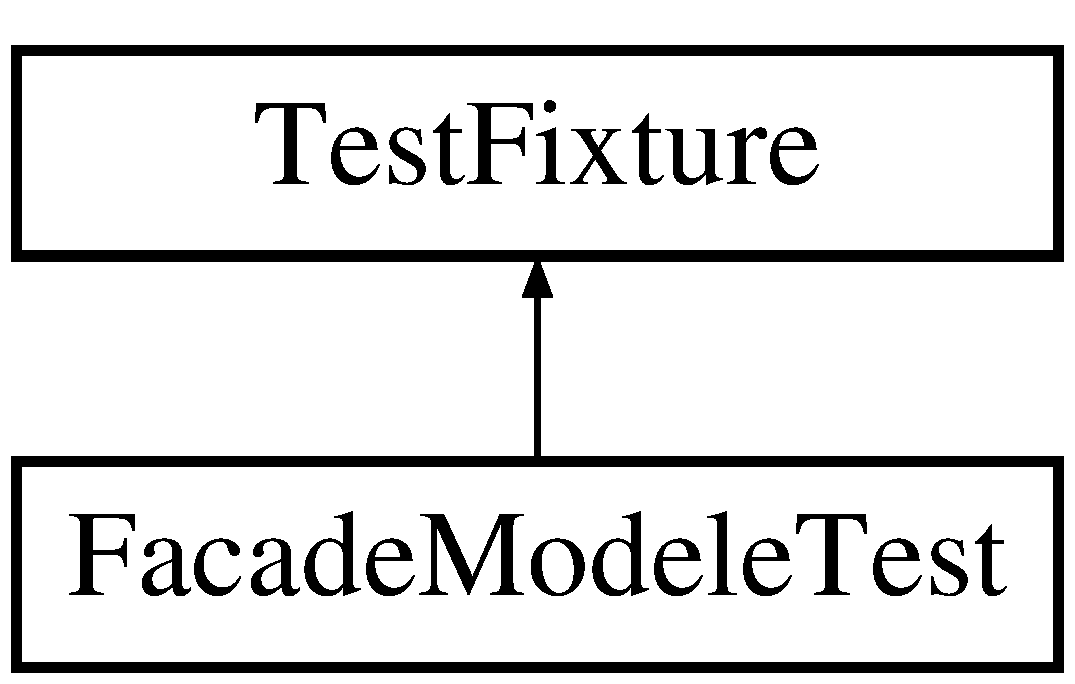
\includegraphics[height=2.000000cm]{class_facade_modele_test}
\end{center}
\end{figure}
\subsection*{Fonctions membres publiques}
\begin{DoxyCompactItemize}
\item 
void \hyperlink{group__inf2990_gaee2f8265a20182be11bcf8839311a8d8}{set\-Up} ()
\begin{DoxyCompactList}\small\item\em Traitement à effectuer pour initialiser cette suite de tests. \end{DoxyCompactList}\item 
void \hyperlink{group__inf2990_ga864b95ee45f0949e36b3670ebe6fb7c4}{tear\-Down} ()
\begin{DoxyCompactList}\small\item\em Traitement à effectuer pour 'finaliser' cette suite de tests. \end{DoxyCompactList}\item 
void \hyperlink{group__inf2990_gaddc1a794fa60c4a77818bd7ee7a4defe}{is\-On\-Table\-Test} ()
\begin{DoxyCompactList}\small\item\em Cas de test\-: présence d'un noeud sur la table. \end{DoxyCompactList}\end{DoxyCompactItemize}


\subsection{Description détaillée}
Classe de test cppunit pour tester le bon fonctionnement des méthodes de la classe \hyperlink{class_facade_modele}{Facade\-Modele}. 

\begin{DoxyAuthor}{Auteur}
I\-N\-F2990-\/\-A15-\/01 
\end{DoxyAuthor}
\begin{DoxyDate}{Date}
2015-\/11-\/09 
\end{DoxyDate}


La documentation de cette classe a été générée à partir des fichiers suivants \-:\begin{DoxyCompactItemize}
\item 
C\-:/\-Users/saron/\-Documents/inf2990-\/01/\-Sources/\-D\-L\-L/\-Tests/\hyperlink{_facade_modele_test_8h}{Facade\-Modele\-Test.\-h}\item 
C\-:/\-Users/saron/\-Documents/inf2990-\/01/\-Sources/\-D\-L\-L/\-Tests/\hyperlink{_facade_modele_test_8cpp}{Facade\-Modele\-Test.\-cpp}\end{DoxyCompactItemize}

\hypertarget{class_f_l___steady_fwd}{\section{Référence de la classe F\-L\-\_\-\-Steady\-Fwd}
\label{class_f_l___steady_fwd}\index{F\-L\-\_\-\-Steady\-Fwd@{F\-L\-\_\-\-Steady\-Fwd}}
}


Classe sous-\/etat pour l'etat \char`\"{}\-Follow\-Line\char`\"{}.  




{\ttfamily \#include $<$F\-L\-\_\-\-Steady\-Fwd.\-h$>$}

Graphe d'héritage de F\-L\-\_\-\-Steady\-Fwd\-:\begin{figure}[H]
\begin{center}
\leavevmode
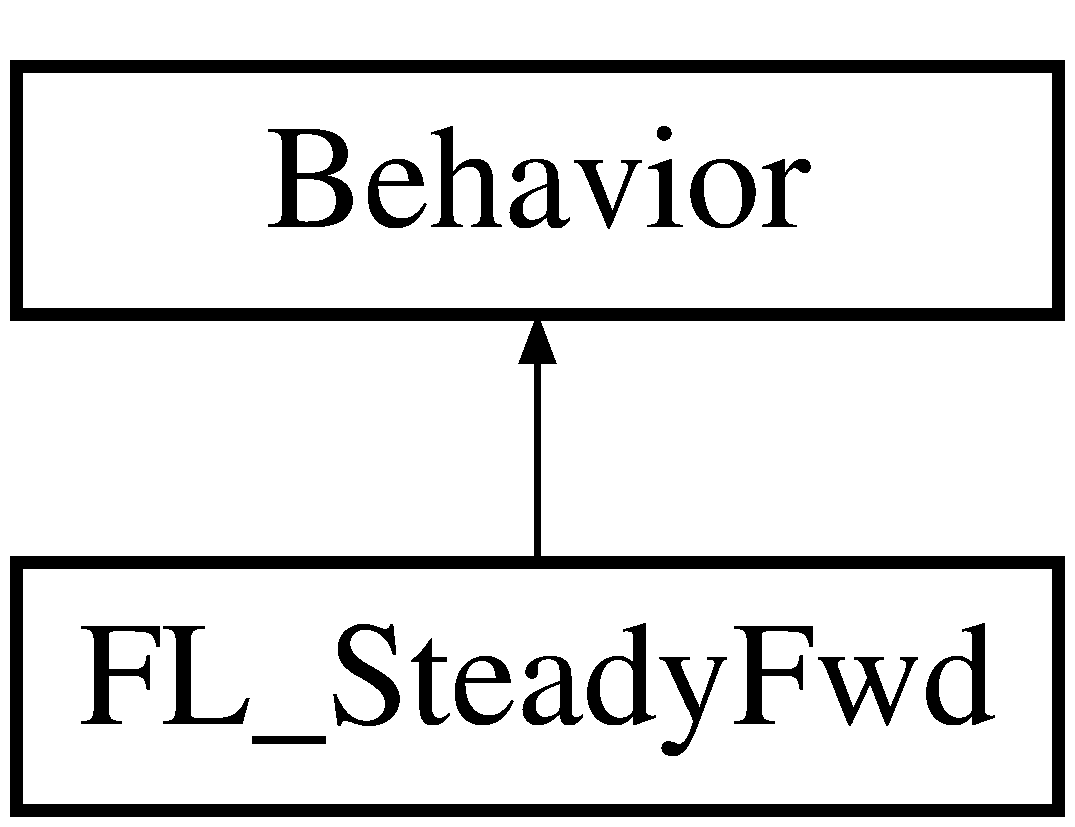
\includegraphics[height=2.000000cm]{class_f_l___steady_fwd}
\end{center}
\end{figure}
\subsection*{Fonctions membres publiques}
{\bf }\par
\begin{DoxyCompactItemize}
\item 
\hyperlink{class_f_l___steady_fwd_aa59ef9cea5b095213ce577971f0613c6}{F\-L\-\_\-\-Steady\-Fwd} (\hyperlink{class_behavior_context}{Behavior\-Context} $\ast$context)
\begin{DoxyCompactList}\small\item\em Constructeur. \end{DoxyCompactList}\item 
void \hyperlink{class_f_l___steady_fwd_a2d1b5496599302e15a292a2547b3226e}{do\-Action} () override
\begin{DoxyCompactList}\small\item\em Effectue une etape de son comportement. \end{DoxyCompactList}\end{DoxyCompactItemize}

\subsection*{Membres hérités additionnels}


\subsection{Description détaillée}
Classe sous-\/etat pour l'etat \char`\"{}\-Follow\-Line\char`\"{}. 

\subsection{Documentation des constructeurs et destructeur}
\hypertarget{class_f_l___steady_fwd_aa59ef9cea5b095213ce577971f0613c6}{\index{F\-L\-\_\-\-Steady\-Fwd@{F\-L\-\_\-\-Steady\-Fwd}!F\-L\-\_\-\-Steady\-Fwd@{F\-L\-\_\-\-Steady\-Fwd}}
\index{F\-L\-\_\-\-Steady\-Fwd@{F\-L\-\_\-\-Steady\-Fwd}!FL_SteadyFwd@{F\-L\-\_\-\-Steady\-Fwd}}
\subsubsection[{F\-L\-\_\-\-Steady\-Fwd}]{\setlength{\rightskip}{0pt plus 5cm}F\-L\-\_\-\-Steady\-Fwd\-::\-F\-L\-\_\-\-Steady\-Fwd (
\begin{DoxyParamCaption}
\item[{{\bf Behavior\-Context} $\ast$}]{context}
\end{DoxyParamCaption}
)}}\label{class_f_l___steady_fwd_aa59ef9cea5b095213ce577971f0613c6}


Constructeur. 

Constructeur


\begin{DoxyParams}[1]{Paramètres}
\mbox{\tt in}  & {\em context} & \-: La classe pouvant accéder au robot.\\
\hline
\end{DoxyParams}
\begin{DoxyReturn}{Renvoie}
Aucune. 
\end{DoxyReturn}


\subsection{Documentation des fonctions membres}
\hypertarget{class_f_l___steady_fwd_a2d1b5496599302e15a292a2547b3226e}{\index{F\-L\-\_\-\-Steady\-Fwd@{F\-L\-\_\-\-Steady\-Fwd}!do\-Action@{do\-Action}}
\index{do\-Action@{do\-Action}!FL_SteadyFwd@{F\-L\-\_\-\-Steady\-Fwd}}
\subsubsection[{do\-Action}]{\setlength{\rightskip}{0pt plus 5cm}void F\-L\-\_\-\-Steady\-Fwd\-::do\-Action (
\begin{DoxyParamCaption}
{}
\end{DoxyParamCaption}
)\hspace{0.3cm}{\ttfamily [override]}, {\ttfamily [virtual]}}}\label{class_f_l___steady_fwd_a2d1b5496599302e15a292a2547b3226e}


Effectue une etape de son comportement. 

Cette fonction effectue le comportement de l'état actuel.


\begin{DoxyParams}[1]{Paramètres}
\mbox{\tt in}  & {\em Aucun.} & \\
\hline
\end{DoxyParams}
\begin{DoxyReturn}{Renvoie}
Aucune. 
\end{DoxyReturn}


Réimplémentée à partir de \hyperlink{group__inf2990_gac22f205bc85075ff707ad1f695c18439}{Behavior}.



La documentation de cette classe a été générée à partir des fichiers suivants \-:\begin{DoxyCompactItemize}
\item 
C\-:/\-Users/saron/\-Documents/inf2990-\/01/\-Sources/\-D\-L\-L/\-Behavior/\hyperlink{_f_l___steady_fwd_8h}{F\-L\-\_\-\-Steady\-Fwd.\-h}\item 
C\-:/\-Users/saron/\-Documents/inf2990-\/01/\-Sources/\-D\-L\-L/\-Behavior/\hyperlink{_f_l___steady_fwd_8cpp}{F\-L\-\_\-\-Steady\-Fwd.\-cpp}\end{DoxyCompactItemize}

\hypertarget{class_f_l___steady_left}{\section{Référence de la classe F\-L\-\_\-\-Steady\-Left}
\label{class_f_l___steady_left}\index{F\-L\-\_\-\-Steady\-Left@{F\-L\-\_\-\-Steady\-Left}}
}


Classe sous-\/etat pour l'etat \char`\"{}\-Follow\-Line\char`\"{}.  




{\ttfamily \#include $<$F\-L\-\_\-\-Steady\-Left.\-h$>$}

Graphe d'héritage de F\-L\-\_\-\-Steady\-Left\-:\begin{figure}[H]
\begin{center}
\leavevmode
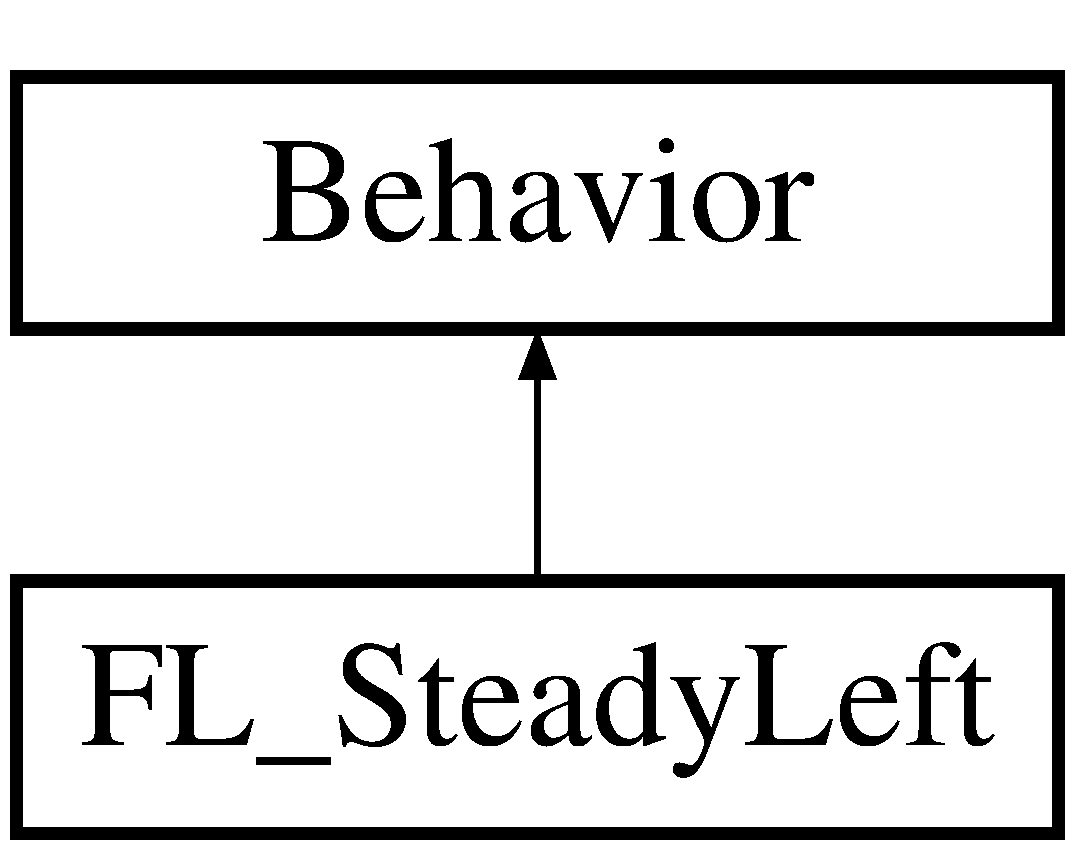
\includegraphics[height=2.000000cm]{class_f_l___steady_left}
\end{center}
\end{figure}
\subsection*{Fonctions membres publiques}
{\bf }\par
\begin{DoxyCompactItemize}
\item 
\hyperlink{class_f_l___steady_left_a99360fe370bf684a4000eb8147292a2b}{F\-L\-\_\-\-Steady\-Left} (\hyperlink{class_behavior_context}{Behavior\-Context} $\ast$context)
\begin{DoxyCompactList}\small\item\em Constructeur. \end{DoxyCompactList}\item 
void \hyperlink{class_f_l___steady_left_aa549ba6f52214d98054caea705f043b5}{do\-Action} () override
\begin{DoxyCompactList}\small\item\em Effectue une etape de son comportement. \end{DoxyCompactList}\end{DoxyCompactItemize}

\subsection*{Membres hérités additionnels}


\subsection{Description détaillée}
Classe sous-\/etat pour l'etat \char`\"{}\-Follow\-Line\char`\"{}. 

\subsection{Documentation des constructeurs et destructeur}
\hypertarget{class_f_l___steady_left_a99360fe370bf684a4000eb8147292a2b}{\index{F\-L\-\_\-\-Steady\-Left@{F\-L\-\_\-\-Steady\-Left}!F\-L\-\_\-\-Steady\-Left@{F\-L\-\_\-\-Steady\-Left}}
\index{F\-L\-\_\-\-Steady\-Left@{F\-L\-\_\-\-Steady\-Left}!FL_SteadyLeft@{F\-L\-\_\-\-Steady\-Left}}
\subsubsection[{F\-L\-\_\-\-Steady\-Left}]{\setlength{\rightskip}{0pt plus 5cm}F\-L\-\_\-\-Steady\-Left\-::\-F\-L\-\_\-\-Steady\-Left (
\begin{DoxyParamCaption}
\item[{{\bf Behavior\-Context} $\ast$}]{context}
\end{DoxyParamCaption}
)}}\label{class_f_l___steady_left_a99360fe370bf684a4000eb8147292a2b}


Constructeur. 

Constructeur


\begin{DoxyParams}[1]{Paramètres}
\mbox{\tt in}  & {\em context} & \-: La classe pouvant accéder au robot.\\
\hline
\end{DoxyParams}
\begin{DoxyReturn}{Renvoie}
Aucune. 
\end{DoxyReturn}


\subsection{Documentation des fonctions membres}
\hypertarget{class_f_l___steady_left_aa549ba6f52214d98054caea705f043b5}{\index{F\-L\-\_\-\-Steady\-Left@{F\-L\-\_\-\-Steady\-Left}!do\-Action@{do\-Action}}
\index{do\-Action@{do\-Action}!FL_SteadyLeft@{F\-L\-\_\-\-Steady\-Left}}
\subsubsection[{do\-Action}]{\setlength{\rightskip}{0pt plus 5cm}void F\-L\-\_\-\-Steady\-Left\-::do\-Action (
\begin{DoxyParamCaption}
{}
\end{DoxyParamCaption}
)\hspace{0.3cm}{\ttfamily [override]}, {\ttfamily [virtual]}}}\label{class_f_l___steady_left_aa549ba6f52214d98054caea705f043b5}


Effectue une etape de son comportement. 

Cette fonction effectue le comportement de l'état actuel.


\begin{DoxyParams}[1]{Paramètres}
\mbox{\tt in}  & {\em Aucun.} & \\
\hline
\end{DoxyParams}
\begin{DoxyReturn}{Renvoie}
Aucune. 
\end{DoxyReturn}


Réimplémentée à partir de \hyperlink{group__inf2990_gac22f205bc85075ff707ad1f695c18439}{Behavior}.



La documentation de cette classe a été générée à partir des fichiers suivants \-:\begin{DoxyCompactItemize}
\item 
C\-:/\-Users/saron/\-Documents/inf2990-\/01/\-Sources/\-D\-L\-L/\-Behavior/\hyperlink{_f_l___steady_left_8h}{F\-L\-\_\-\-Steady\-Left.\-h}\item 
C\-:/\-Users/saron/\-Documents/inf2990-\/01/\-Sources/\-D\-L\-L/\-Behavior/\hyperlink{_f_l___steady_left_8cpp}{F\-L\-\_\-\-Steady\-Left.\-cpp}\end{DoxyCompactItemize}

\hypertarget{class_f_l___steady_right}{\section{Référence de la classe F\-L\-\_\-\-Steady\-Right}
\label{class_f_l___steady_right}\index{F\-L\-\_\-\-Steady\-Right@{F\-L\-\_\-\-Steady\-Right}}
}


Classe sous-\/etat pour l'etat \char`\"{}\-Follow\-Line\char`\"{}.  




{\ttfamily \#include $<$F\-L\-\_\-\-Steady\-Right.\-h$>$}

Graphe d'héritage de F\-L\-\_\-\-Steady\-Right\-:\begin{figure}[H]
\begin{center}
\leavevmode
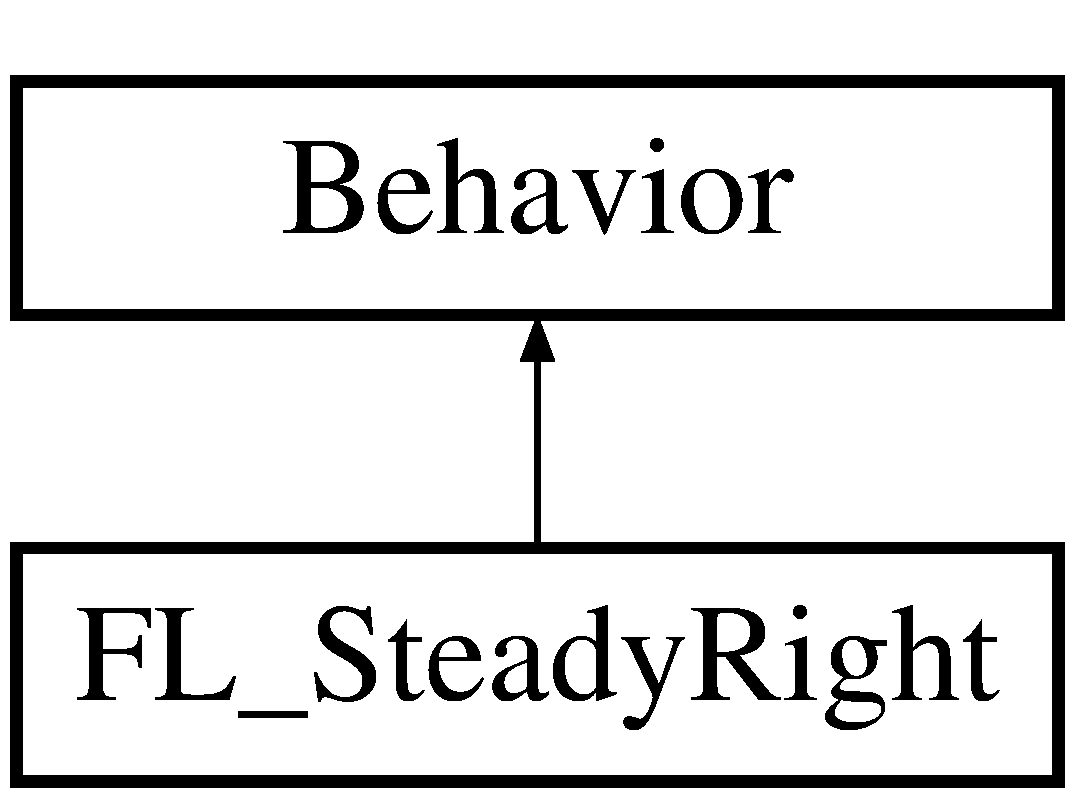
\includegraphics[height=2.000000cm]{class_f_l___steady_right}
\end{center}
\end{figure}
\subsection*{Fonctions membres publiques}
{\bf }\par
\begin{DoxyCompactItemize}
\item 
\hyperlink{class_f_l___steady_right_ab030ddf91a8ff28074b6f7997058354a}{F\-L\-\_\-\-Steady\-Right} (\hyperlink{class_behavior_context}{Behavior\-Context} $\ast$context)
\begin{DoxyCompactList}\small\item\em Constructeur. \end{DoxyCompactList}\item 
void \hyperlink{class_f_l___steady_right_a6d27554021510b8cfdf757d06f8b4e90}{do\-Action} () override
\begin{DoxyCompactList}\small\item\em Effectue une etape de son comportement. \end{DoxyCompactList}\end{DoxyCompactItemize}

\subsection*{Membres hérités additionnels}


\subsection{Description détaillée}
Classe sous-\/etat pour l'etat \char`\"{}\-Follow\-Line\char`\"{}. 

\subsection{Documentation des constructeurs et destructeur}
\hypertarget{class_f_l___steady_right_ab030ddf91a8ff28074b6f7997058354a}{\index{F\-L\-\_\-\-Steady\-Right@{F\-L\-\_\-\-Steady\-Right}!F\-L\-\_\-\-Steady\-Right@{F\-L\-\_\-\-Steady\-Right}}
\index{F\-L\-\_\-\-Steady\-Right@{F\-L\-\_\-\-Steady\-Right}!FL_SteadyRight@{F\-L\-\_\-\-Steady\-Right}}
\subsubsection[{F\-L\-\_\-\-Steady\-Right}]{\setlength{\rightskip}{0pt plus 5cm}F\-L\-\_\-\-Steady\-Right\-::\-F\-L\-\_\-\-Steady\-Right (
\begin{DoxyParamCaption}
\item[{{\bf Behavior\-Context} $\ast$}]{context}
\end{DoxyParamCaption}
)}}\label{class_f_l___steady_right_ab030ddf91a8ff28074b6f7997058354a}


Constructeur. 

Constructeur


\begin{DoxyParams}[1]{Paramètres}
\mbox{\tt in}  & {\em context} & \-: La classe pouvant accéder au robot.\\
\hline
\end{DoxyParams}
\begin{DoxyReturn}{Renvoie}
Aucune. 
\end{DoxyReturn}


\subsection{Documentation des fonctions membres}
\hypertarget{class_f_l___steady_right_a6d27554021510b8cfdf757d06f8b4e90}{\index{F\-L\-\_\-\-Steady\-Right@{F\-L\-\_\-\-Steady\-Right}!do\-Action@{do\-Action}}
\index{do\-Action@{do\-Action}!FL_SteadyRight@{F\-L\-\_\-\-Steady\-Right}}
\subsubsection[{do\-Action}]{\setlength{\rightskip}{0pt plus 5cm}void F\-L\-\_\-\-Steady\-Right\-::do\-Action (
\begin{DoxyParamCaption}
{}
\end{DoxyParamCaption}
)\hspace{0.3cm}{\ttfamily [override]}, {\ttfamily [virtual]}}}\label{class_f_l___steady_right_a6d27554021510b8cfdf757d06f8b4e90}


Effectue une etape de son comportement. 

Cette fonction effectue le comportement de l'état actuel.


\begin{DoxyParams}[1]{Paramètres}
\mbox{\tt in}  & {\em Aucun.} & \\
\hline
\end{DoxyParams}
\begin{DoxyReturn}{Renvoie}
Aucune. 
\end{DoxyReturn}


Réimplémentée à partir de \hyperlink{group__inf2990_gac22f205bc85075ff707ad1f695c18439}{Behavior}.



La documentation de cette classe a été générée à partir des fichiers suivants \-:\begin{DoxyCompactItemize}
\item 
C\-:/\-Users/saron/\-Documents/inf2990-\/01/\-Sources/\-D\-L\-L/\-Behavior/\hyperlink{_f_l___steady_right_8h}{F\-L\-\_\-\-Steady\-Right.\-h}\item 
C\-:/\-Users/saron/\-Documents/inf2990-\/01/\-Sources/\-D\-L\-L/\-Behavior/\hyperlink{_f_l___steady_right_8cpp}{F\-L\-\_\-\-Steady\-Right.\-cpp}\end{DoxyCompactItemize}

\hypertarget{class_follow_line}{\section{Référence de la classe Follow\-Line}
\label{class_follow_line}\index{Follow\-Line@{Follow\-Line}}
}


Classe Etat du comportement \char`\"{}\-Suivi de ligne\char`\"{}.  




{\ttfamily \#include $<$Follow\-Line.\-h$>$}

Graphe d'héritage de Follow\-Line\-:\begin{figure}[H]
\begin{center}
\leavevmode
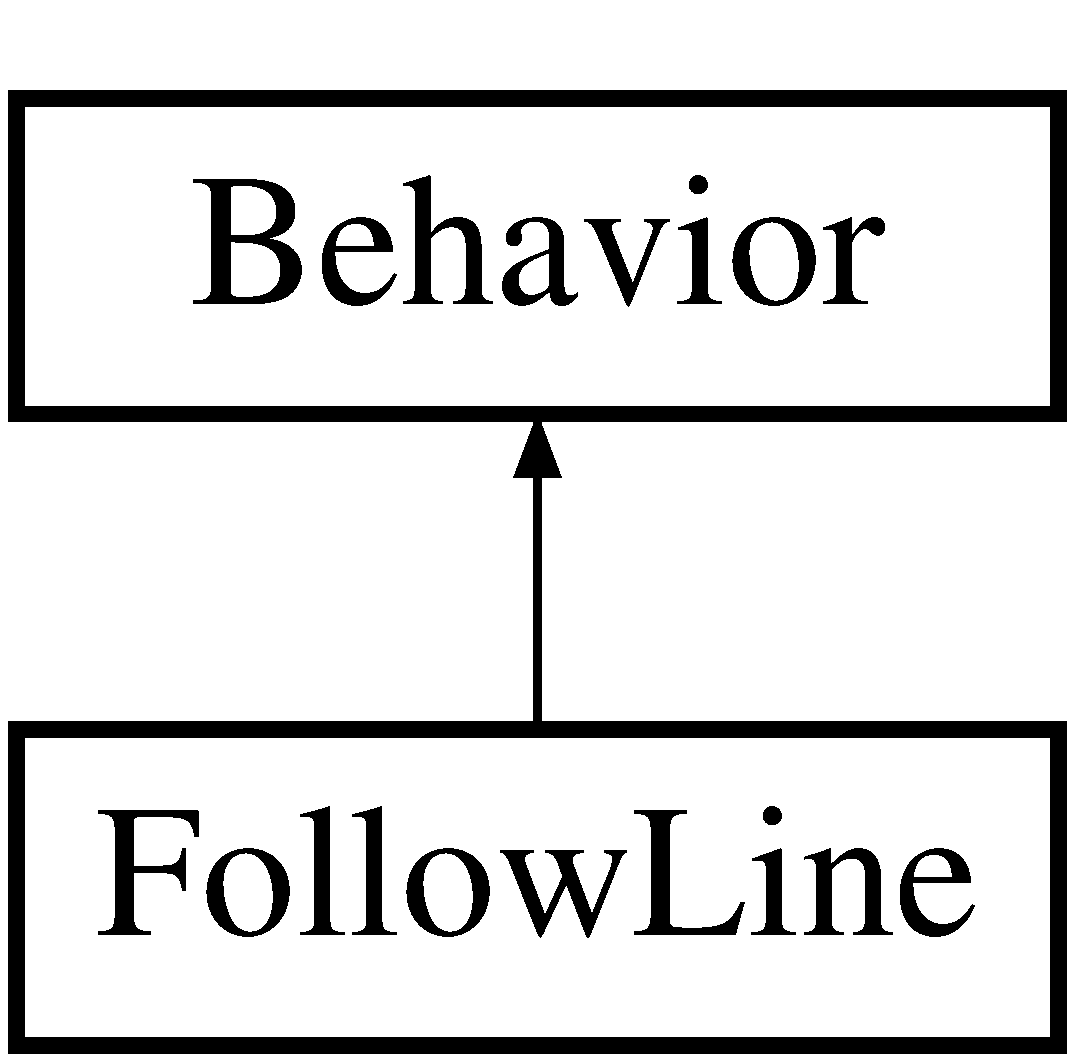
\includegraphics[height=2.000000cm]{class_follow_line}
\end{center}
\end{figure}
\subsection*{Fonctions membres publiques}
\begin{DoxyCompactItemize}
\item 
\hypertarget{class_follow_line_a4605773b98e3407e1f4251f7525bf20b}{\hyperlink{class_follow_line_a4605773b98e3407e1f4251f7525bf20b}{Follow\-Line} (\hyperlink{class_behavior_context}{Behavior\-Context} $\ast$context)}\label{class_follow_line_a4605773b98e3407e1f4251f7525bf20b}

\begin{DoxyCompactList}\small\item\em Constructeur. \end{DoxyCompactList}\end{DoxyCompactItemize}
{\bf }\par
\begin{DoxyCompactItemize}
\item 
void \hyperlink{class_follow_line_ad85edb064ae36be3860e376c9681655d}{do\-Action} () override
\begin{DoxyCompactList}\small\item\em Effectue une etape de son comportement. \end{DoxyCompactList}\end{DoxyCompactItemize}

\subsection*{Membres hérités additionnels}


\subsection{Description détaillée}
Classe Etat du comportement \char`\"{}\-Suivi de ligne\char`\"{}. 

\subsection{Documentation des fonctions membres}
\hypertarget{class_follow_line_ad85edb064ae36be3860e376c9681655d}{\index{Follow\-Line@{Follow\-Line}!do\-Action@{do\-Action}}
\index{do\-Action@{do\-Action}!FollowLine@{Follow\-Line}}
\subsubsection[{do\-Action}]{\setlength{\rightskip}{0pt plus 5cm}void Follow\-Line\-::do\-Action (
\begin{DoxyParamCaption}
{}
\end{DoxyParamCaption}
)\hspace{0.3cm}{\ttfamily [override]}, {\ttfamily [virtual]}}}\label{class_follow_line_ad85edb064ae36be3860e376c9681655d}


Effectue une etape de son comportement. 

Cette fonction effectue le comportement de l'état actuel.


\begin{DoxyParams}[1]{Paramètres}
\mbox{\tt in}  & {\em Aucun.} & \\
\hline
\end{DoxyParams}
\begin{DoxyReturn}{Renvoie}
Aucune. 
\end{DoxyReturn}


Réimplémentée à partir de \hyperlink{group__inf2990_gac22f205bc85075ff707ad1f695c18439}{Behavior}.



La documentation de cette classe a été générée à partir des fichiers suivants \-:\begin{DoxyCompactItemize}
\item 
C\-:/\-Users/saron/\-Documents/inf2990-\/01/\-Sources/\-D\-L\-L/\-Behavior/\hyperlink{_follow_line_8h}{Follow\-Line.\-h}\item 
C\-:/\-Users/saron/\-Documents/inf2990-\/01/\-Sources/\-D\-L\-L/\-Behavior/\hyperlink{_follow_line_8cpp}{Follow\-Line.\-cpp}\end{DoxyCompactItemize}

\hypertarget{class_get_data_tool}{}\section{Get\+Data\+Tool Class Reference}
\label{class_get_data_tool}\index{Get\+Data\+Tool@{Get\+Data\+Tool}}


Classe concrète héritant de \hyperlink{class_tool}{Tool}, qui prend les données du noeud sélectionné  




{\ttfamily \#include $<$Get\+Data\+Tool.\+h$>$}

Inheritance diagram for Get\+Data\+Tool\+:\begin{figure}[H]
\begin{center}
\leavevmode
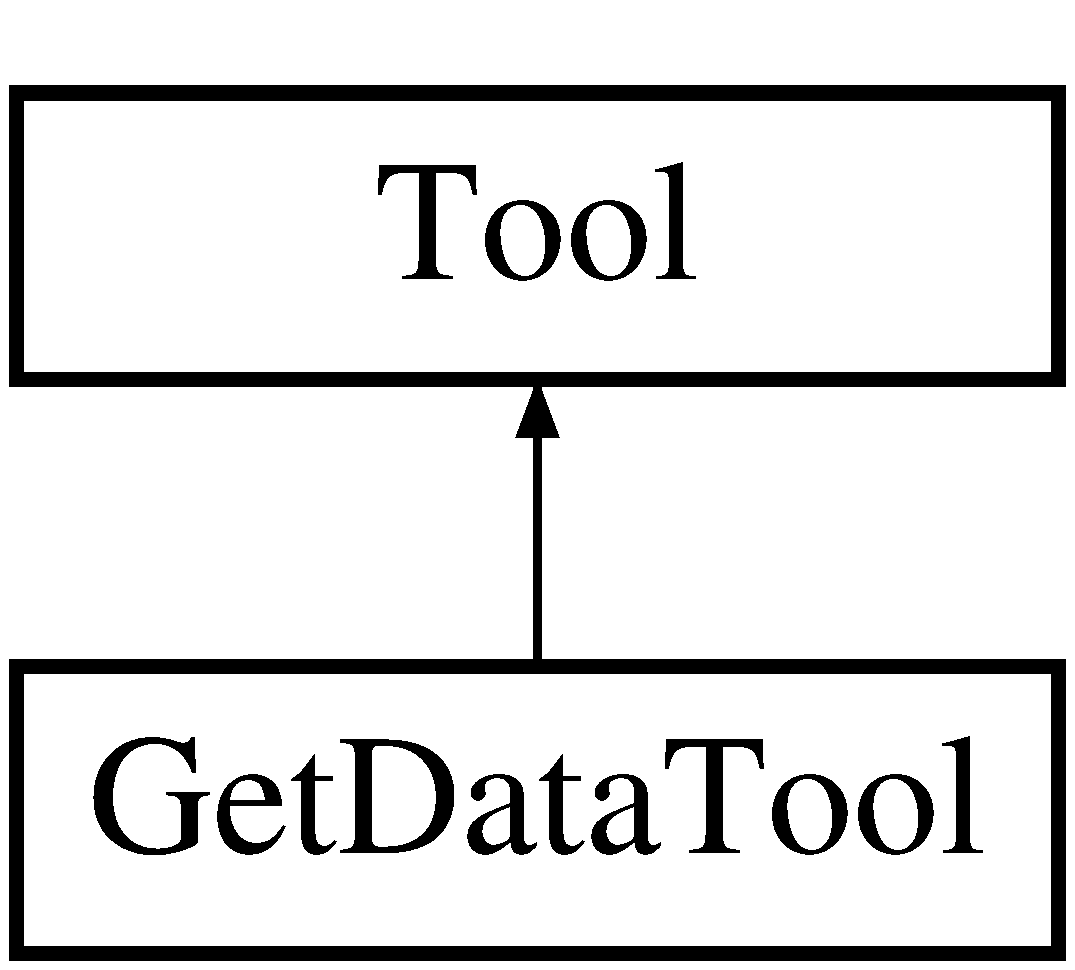
\includegraphics[height=2.000000cm]{class_get_data_tool}
\end{center}
\end{figure}
\subsection*{Public Member Functions}
\begin{DoxyCompactItemize}
\item 
\hypertarget{class_get_data_tool_a9812d5218ecf28b18dbd8ae8180e98f6}{}{\bfseries Get\+Data\+Tool} (\hyperlink{struct_node_properties}{Node\+Properties} $\ast$data)\label{class_get_data_tool_a9812d5218ecf28b18dbd8ae8180e98f6}

\item 
void \hyperlink{group__inf2990_ga21292ea905abc9e5c85d04e4ca9b6863}{visit} (\hyperlink{class_noeud_cylindre}{Noeud\+Cylindre} $\ast$node) override
\item 
void \hyperlink{group__inf2990_ga4ce08dbc70076e50ec519cd082a9e1ad}{visit} (\hyperlink{class_noeud_depart}{Noeud\+Depart} $\ast$node) override
\item 
void \hyperlink{group__inf2990_gadac537c2e9d4cf9b5d27695f497f7b1d}{visit} (\hyperlink{class_noeud_ligne}{Noeud\+Ligne} $\ast$node) override
\item 
void \hyperlink{group__inf2990_ga9db0192f32035edd1e4b8c2858feb5d1}{visit} (\hyperlink{class_noeud_mur}{Noeud\+Mur} $\ast$node) override
\item 
void \hyperlink{group__inf2990_gab96d72787632de185fd46dee5d8b9750}{default\+Getter} (\hyperlink{class_noeud_abstrait}{Noeud\+Abstrait} $\ast$node)
\end{DoxyCompactItemize}


\subsection{Detailed Description}
Classe concrète héritant de \hyperlink{class_tool}{Tool}, qui prend les données du noeud sélectionné 

\begin{DoxyAuthor}{Author}
I\+N\+F2990-\/\+A15-\/01 
\end{DoxyAuthor}
\begin{DoxyDate}{Date}
2015-\/09-\/14 
\end{DoxyDate}


The documentation for this class was generated from the following files\+:\begin{DoxyCompactItemize}
\item 
Sources/\+D\+L\+L/\+Application/\+Visitor/\hyperlink{_get_data_tool_8h}{Get\+Data\+Tool.\+h}\item 
Sources/\+D\+L\+L/\+Application/\+Visitor/\hyperlink{_get_data_tool_8cpp}{Get\+Data\+Tool.\+cpp}\end{DoxyCompactItemize}

\hypertarget{class_interface_graphique_1_1_help_window}{}\section{Interface\+Graphique.\+Help\+Window Class Reference}
\label{class_interface_graphique_1_1_help_window}\index{Interface\+Graphique.\+Help\+Window@{Interface\+Graphique.\+Help\+Window}}


Interaction logic for Help\+Window.\+xaml  


Inheritance diagram for Interface\+Graphique.\+Help\+Window\+:\begin{figure}[H]
\begin{center}
\leavevmode
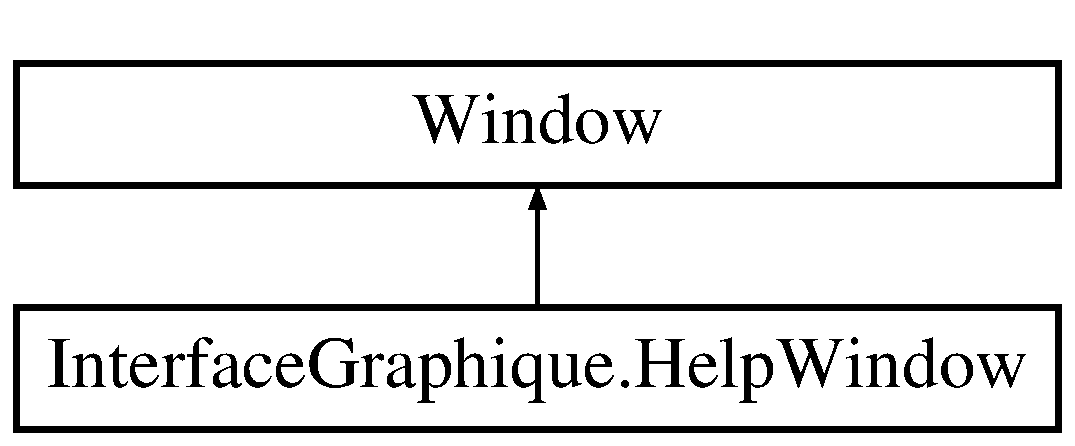
\includegraphics[height=2.000000cm]{class_interface_graphique_1_1_help_window}
\end{center}
\end{figure}


\subsection{Detailed Description}
Interaction logic for Help\+Window.\+xaml 



The documentation for this class was generated from the following file\+:\begin{DoxyCompactItemize}
\item 
Sources/\+Interface\+Graphique/Help\+Window.\+xaml.\+cs\end{DoxyCompactItemize}

\hypertarget{class_invalid_tool}{}\section{Invalid\+Tool Class Reference}
\label{class_invalid_tool}\index{Invalid\+Tool@{Invalid\+Tool}}
Inheritance diagram for Invalid\+Tool\+:\begin{figure}[H]
\begin{center}
\leavevmode
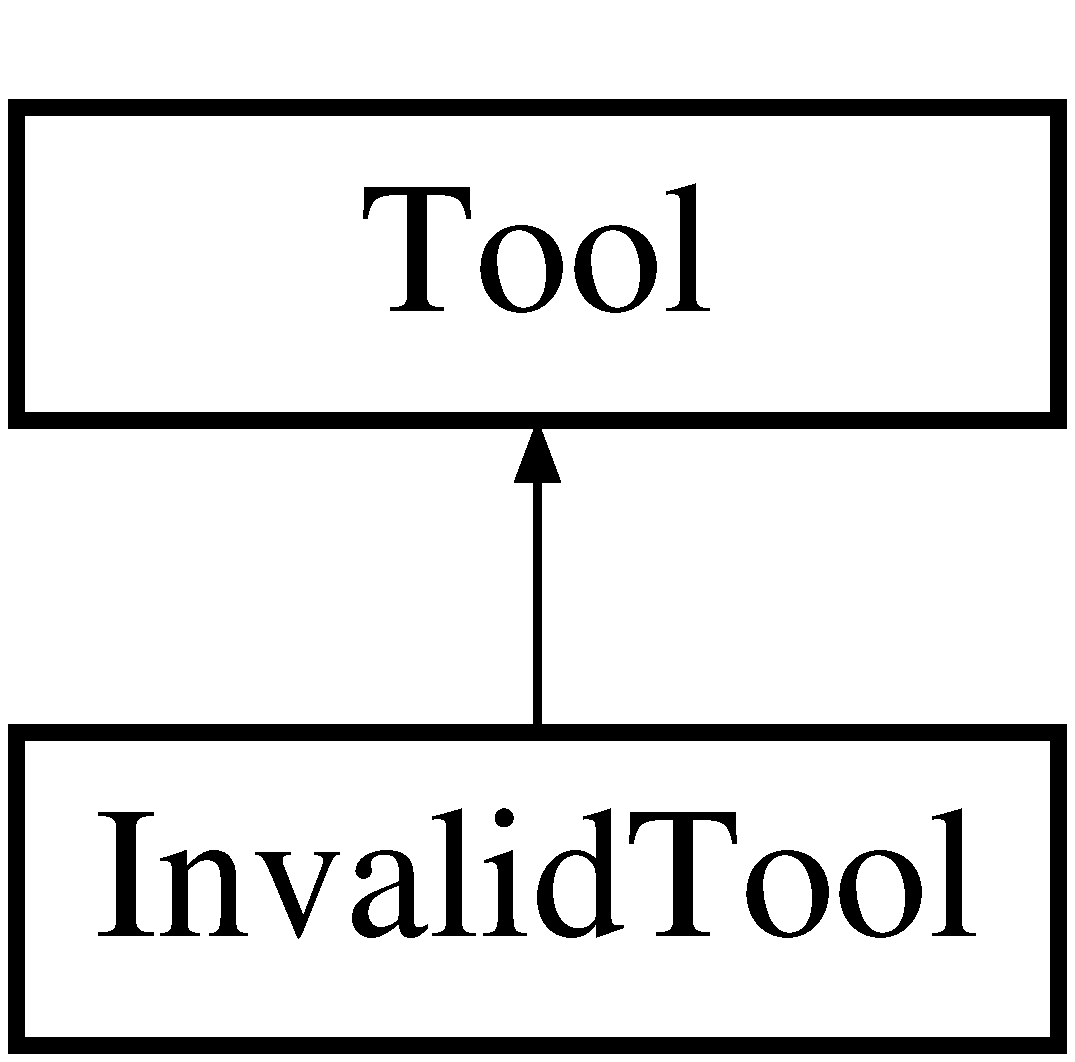
\includegraphics[height=2.000000cm]{class_invalid_tool}
\end{center}
\end{figure}
\subsection*{Public Member Functions}
\begin{DoxyCompactItemize}
\item 
void \hyperlink{group__inf2990_ga55674ebdcf4c31ced5df732e2424d282}{visit} (\hyperlink{class_noeud_cylindre}{Noeud\+Cylindre} $\ast$node) override
\item 
void \hyperlink{group__inf2990_gabbc70a0da4b0aadac5a37f1fce30cb7a}{visit} (\hyperlink{class_noeud_depart}{Noeud\+Depart} $\ast$node) override
\item 
void \hyperlink{group__inf2990_ga2f8397c63d7f895906f49ab95de03f13}{visit} (\hyperlink{class_noeud_segment_concret}{Noeud\+Segment\+Concret} $\ast$node) override
\item 
void \hyperlink{group__inf2990_gab69a438cb8d2abff211cd450c9f946f5}{visit} (\hyperlink{class_noeud_mur}{Noeud\+Mur} $\ast$node) override
\end{DoxyCompactItemize}
\subsection*{Protected Member Functions}
\begin{DoxyCompactItemize}
\item 
void \hyperlink{group__inf2990_gafb96baa12cb0df8c48c84dd12badd757}{default\+Invalid} (\hyperlink{class_noeud_abstrait}{Noeud\+Abstrait} $\ast$node)
\begin{DoxyCompactList}\small\item\em Algorithme par défaut. \end{DoxyCompactList}\end{DoxyCompactItemize}


The documentation for this class was generated from the following files\+:\begin{DoxyCompactItemize}
\item 
Sources/\+D\+L\+L/\+Application/\+Visitor/\hyperlink{_invalid_tool_8h}{Invalid\+Tool.\+h}\item 
Sources/\+D\+L\+L/\+Application/\+Visitor/\hyperlink{_invalid_tool_8cpp}{Invalid\+Tool.\+cpp}\end{DoxyCompactItemize}

\hypertarget{class_interface_graphique_1_1_key_bindings}{\section{Référence de la classe Interface\-Graphique.\-Key\-Bindings}
\label{class_interface_graphique_1_1_key_bindings}\index{Interface\-Graphique.\-Key\-Bindings@{Interface\-Graphique.\-Key\-Bindings}}
}
\subsection*{Propriétés}
\begin{DoxyCompactItemize}
\item 
\hypertarget{class_interface_graphique_1_1_key_bindings_acfba3a6fd83fc49f186c52acdb2291df}{String {\bfseries Forward}\hspace{0.3cm}{\ttfamily  \mbox{[}get, set\mbox{]}}}\label{class_interface_graphique_1_1_key_bindings_acfba3a6fd83fc49f186c52acdb2291df}

\item 
\hypertarget{class_interface_graphique_1_1_key_bindings_a6bb6e71fe377c5da46d56e9f3cc2dc64}{String {\bfseries Reverse}\hspace{0.3cm}{\ttfamily  \mbox{[}get, set\mbox{]}}}\label{class_interface_graphique_1_1_key_bindings_a6bb6e71fe377c5da46d56e9f3cc2dc64}

\item 
\hypertarget{class_interface_graphique_1_1_key_bindings_a463af07de4227307c63e6a0b3265a6bc}{String {\bfseries Turn\-Right}\hspace{0.3cm}{\ttfamily  \mbox{[}get, set\mbox{]}}}\label{class_interface_graphique_1_1_key_bindings_a463af07de4227307c63e6a0b3265a6bc}

\item 
\hypertarget{class_interface_graphique_1_1_key_bindings_a0520e1d4136842d65e21450d988fc5f3}{String {\bfseries Turn\-Left}\hspace{0.3cm}{\ttfamily  \mbox{[}get, set\mbox{]}}}\label{class_interface_graphique_1_1_key_bindings_a0520e1d4136842d65e21450d988fc5f3}

\item 
\hypertarget{class_interface_graphique_1_1_key_bindings_abd885c126538991eea0db3efcd37ede6}{String {\bfseries Toggle}\hspace{0.3cm}{\ttfamily  \mbox{[}get, set\mbox{]}}}\label{class_interface_graphique_1_1_key_bindings_abd885c126538991eea0db3efcd37ede6}

\end{DoxyCompactItemize}


La documentation de cette classe a été générée à partir du fichier suivant \-:\begin{DoxyCompactItemize}
\item 
C\-:/\-Users/saron/\-Documents/inf2990-\/01/\-Sources/\-Interface\-Graphique/Key\-Bindings.\-cs\end{DoxyCompactItemize}

\hypertarget{classaidegl_1_1_ligne_pointillee}{\section{Référence de la classe aidegl\-:\-:Ligne\-Pointillee}
\label{classaidegl_1_1_ligne_pointillee}\index{aidegl\-::\-Ligne\-Pointillee@{aidegl\-::\-Ligne\-Pointillee}}
}


Classe qui gère l'affichage de lignes pointillées.  




{\ttfamily \#include $<$Ligne\-Pointillee.\-h$>$}

\subsection*{Fonctions membres publiques}
\begin{DoxyCompactItemize}
\item 
\hyperlink{classaidegl_1_1_ligne_pointillee_a4fc590690c8bbc7368fb355a71d5eaf2}{Ligne\-Pointillee} ()
\begin{DoxyCompactList}\small\item\em Constructeur par defaut. \end{DoxyCompactList}\item 
void \hyperlink{classaidegl_1_1_ligne_pointillee_a455e3f5a717d72b04808c90c3d20f23f}{commencer} () const 
\begin{DoxyCompactList}\small\item\em Début du rendu de lignes. \end{DoxyCompactList}\item 
void \hyperlink{classaidegl_1_1_ligne_pointillee_a5a1522b90f6970b3a33103935bed74da}{finir} () const 
\begin{DoxyCompactList}\small\item\em Fin du rendu de lignes. \end{DoxyCompactList}\item 
void \hyperlink{classaidegl_1_1_ligne_pointillee_a73fc1d54bcd3afd2861ea81a8b3721d0}{assigner\-Couleur} (const glm\-::fvec4 \&couleur)
\begin{DoxyCompactList}\small\item\em Assigne la couleur des lignes. \end{DoxyCompactList}\item 
void \hyperlink{classaidegl_1_1_ligne_pointillee_a0d9e3b0ca2604f1e9410b868a8917a78}{assigner\-Facteur} (int facteur)
\begin{DoxyCompactList}\small\item\em Assigne le facteur multiplicatif du pointillé. \end{DoxyCompactList}\item 
void \hyperlink{classaidegl_1_1_ligne_pointillee_a2eb75fea1bec5566ca4feae3612d7b5e}{assigner\-Patron} (unsigned short patron)
\begin{DoxyCompactList}\small\item\em Assigne le patron de pointillé des lignes. \end{DoxyCompactList}\end{DoxyCompactItemize}


\subsection{Description détaillée}
Classe qui gère l'affichage de lignes pointillées. 

\begin{DoxyAuthor}{Auteur}
Martin Bisson 
\end{DoxyAuthor}
\begin{DoxyDate}{Date}
2007-\/01-\/28 
\end{DoxyDate}


\subsection{Documentation des constructeurs et destructeur}
\hypertarget{classaidegl_1_1_ligne_pointillee_a4fc590690c8bbc7368fb355a71d5eaf2}{\index{aidegl\-::\-Ligne\-Pointillee@{aidegl\-::\-Ligne\-Pointillee}!Ligne\-Pointillee@{Ligne\-Pointillee}}
\index{Ligne\-Pointillee@{Ligne\-Pointillee}!aidegl::LignePointillee@{aidegl\-::\-Ligne\-Pointillee}}
\subsubsection[{Ligne\-Pointillee}]{\setlength{\rightskip}{0pt plus 5cm}aidegl\-::\-Ligne\-Pointillee\-::\-Ligne\-Pointillee (
\begin{DoxyParamCaption}
{}
\end{DoxyParamCaption}
)\hspace{0.3cm}{\ttfamily [inline]}}}\label{classaidegl_1_1_ligne_pointillee_a4fc590690c8bbc7368fb355a71d5eaf2}


Constructeur par defaut. 

Constructeur par défaut qui se contente d'initialiser les paramètres du rendu de la ligne à des valeurs par défaut.

\begin{DoxyReturn}{Renvoie}
Aucune (constructeur). 
\end{DoxyReturn}


\subsection{Documentation des fonctions membres}
\hypertarget{classaidegl_1_1_ligne_pointillee_a73fc1d54bcd3afd2861ea81a8b3721d0}{\index{aidegl\-::\-Ligne\-Pointillee@{aidegl\-::\-Ligne\-Pointillee}!assigner\-Couleur@{assigner\-Couleur}}
\index{assigner\-Couleur@{assigner\-Couleur}!aidegl::LignePointillee@{aidegl\-::\-Ligne\-Pointillee}}
\subsubsection[{assigner\-Couleur}]{\setlength{\rightskip}{0pt plus 5cm}void aidegl\-::\-Ligne\-Pointillee\-::assigner\-Couleur (
\begin{DoxyParamCaption}
\item[{const glm\-::fvec4 \&}]{couleur}
\end{DoxyParamCaption}
)\hspace{0.3cm}{\ttfamily [inline]}}}\label{classaidegl_1_1_ligne_pointillee_a73fc1d54bcd3afd2861ea81a8b3721d0}


Assigne la couleur des lignes. 

Cette fonction permet d'assigner la couleur utilisée pour dessiner les lignes.


\begin{DoxyParams}[1]{Paramètres}
\mbox{\tt in}  & {\em couleur} & \-: La couleur des lignes.\\
\hline
\end{DoxyParams}
\begin{DoxyReturn}{Renvoie}
Aucune. 
\end{DoxyReturn}
\hypertarget{classaidegl_1_1_ligne_pointillee_a0d9e3b0ca2604f1e9410b868a8917a78}{\index{aidegl\-::\-Ligne\-Pointillee@{aidegl\-::\-Ligne\-Pointillee}!assigner\-Facteur@{assigner\-Facteur}}
\index{assigner\-Facteur@{assigner\-Facteur}!aidegl::LignePointillee@{aidegl\-::\-Ligne\-Pointillee}}
\subsubsection[{assigner\-Facteur}]{\setlength{\rightskip}{0pt plus 5cm}void aidegl\-::\-Ligne\-Pointillee\-::assigner\-Facteur (
\begin{DoxyParamCaption}
\item[{int}]{facteur}
\end{DoxyParamCaption}
)\hspace{0.3cm}{\ttfamily [inline]}}}\label{classaidegl_1_1_ligne_pointillee_a0d9e3b0ca2604f1e9410b868a8917a78}


Assigne le facteur multiplicatif du pointillé. 

Cette fonction permet d'assigner le facteur multiplicatif du pointillé utilisé pour dessiner les lignes.


\begin{DoxyParams}[1]{Paramètres}
\mbox{\tt in}  & {\em facteur} & \-: Le facteur multiplicatif.\\
\hline
\end{DoxyParams}
\begin{DoxyReturn}{Renvoie}
Aucune. 
\end{DoxyReturn}
\hypertarget{classaidegl_1_1_ligne_pointillee_a2eb75fea1bec5566ca4feae3612d7b5e}{\index{aidegl\-::\-Ligne\-Pointillee@{aidegl\-::\-Ligne\-Pointillee}!assigner\-Patron@{assigner\-Patron}}
\index{assigner\-Patron@{assigner\-Patron}!aidegl::LignePointillee@{aidegl\-::\-Ligne\-Pointillee}}
\subsubsection[{assigner\-Patron}]{\setlength{\rightskip}{0pt plus 5cm}void aidegl\-::\-Ligne\-Pointillee\-::assigner\-Patron (
\begin{DoxyParamCaption}
\item[{unsigned short}]{patron}
\end{DoxyParamCaption}
)\hspace{0.3cm}{\ttfamily [inline]}}}\label{classaidegl_1_1_ligne_pointillee_a2eb75fea1bec5566ca4feae3612d7b5e}


Assigne le patron de pointillé des lignes. 

Cette fonction permet d'assigner le patron du pointillé utilisé pour dessiner les lignes.


\begin{DoxyParams}[1]{Paramètres}
\mbox{\tt in}  & {\em patron} & \-: Le patron du pointillé.\\
\hline
\end{DoxyParams}
\begin{DoxyReturn}{Renvoie}
Aucune. 
\end{DoxyReturn}
\hypertarget{classaidegl_1_1_ligne_pointillee_a455e3f5a717d72b04808c90c3d20f23f}{\index{aidegl\-::\-Ligne\-Pointillee@{aidegl\-::\-Ligne\-Pointillee}!commencer@{commencer}}
\index{commencer@{commencer}!aidegl::LignePointillee@{aidegl\-::\-Ligne\-Pointillee}}
\subsubsection[{commencer}]{\setlength{\rightskip}{0pt plus 5cm}void aidegl\-::\-Ligne\-Pointillee\-::commencer (
\begin{DoxyParamCaption}
{}
\end{DoxyParamCaption}
) const\hspace{0.3cm}{\ttfamily [inline]}}}\label{classaidegl_1_1_ligne_pointillee_a455e3f5a717d72b04808c90c3d20f23f}


Début du rendu de lignes. 

Cette fonction assigne les paramètres nécessaires pour le début du rendu de la ligne dans la machine à états Open\-G\-L.

\begin{DoxyReturn}{Renvoie}
Aucune. 
\end{DoxyReturn}
\hypertarget{classaidegl_1_1_ligne_pointillee_a5a1522b90f6970b3a33103935bed74da}{\index{aidegl\-::\-Ligne\-Pointillee@{aidegl\-::\-Ligne\-Pointillee}!finir@{finir}}
\index{finir@{finir}!aidegl::LignePointillee@{aidegl\-::\-Ligne\-Pointillee}}
\subsubsection[{finir}]{\setlength{\rightskip}{0pt plus 5cm}void aidegl\-::\-Ligne\-Pointillee\-::finir (
\begin{DoxyParamCaption}
{}
\end{DoxyParamCaption}
) const\hspace{0.3cm}{\ttfamily [inline]}}}\label{classaidegl_1_1_ligne_pointillee_a5a1522b90f6970b3a33103935bed74da}


Fin du rendu de lignes. 

Cette fonction restaure les paramètres d'avant le début du tracé des lignes.

\begin{DoxyReturn}{Renvoie}
Aucune. 
\end{DoxyReturn}


La documentation de cette classe a été générée à partir du fichier suivant \-:\begin{DoxyCompactItemize}
\item 
C\-:/\-Users/saron/\-Documents/inf2990-\/01/\-Commun/\-Utilitaire/\hyperlink{_ligne_pointillee_8h}{Ligne\-Pointillee.\-h}\end{DoxyCompactItemize}

\hypertarget{class_interface_graphique_1_1_main_menu}{}\section{Interface\+Graphique.\+Main\+Menu Class Reference}
\label{class_interface_graphique_1_1_main_menu}\index{Interface\+Graphique.\+Main\+Menu@{Interface\+Graphique.\+Main\+Menu}}


Interaction logic for Main\+Menu.\+xaml  


Inheritance diagram for Interface\+Graphique.\+Main\+Menu\+:\begin{figure}[H]
\begin{center}
\leavevmode
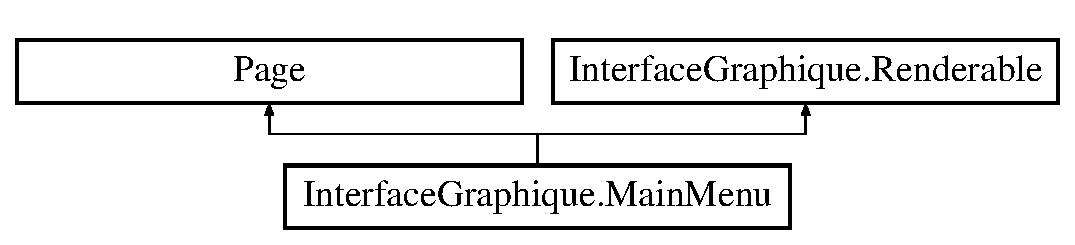
\includegraphics[height=2.000000cm]{class_interface_graphique_1_1_main_menu}
\end{center}
\end{figure}
\subsection*{Public Member Functions}
\begin{DoxyCompactItemize}
\item 
\hypertarget{class_interface_graphique_1_1_main_menu_a5f5f0df5c4abb8f172887e8b307dc32d}{}delegate void {\bfseries Click\+Event\+Handler} (object sender, Event\+Args e)\label{class_interface_graphique_1_1_main_menu_a5f5f0df5c4abb8f172887e8b307dc32d}

\item 
\hypertarget{class_interface_graphique_1_1_main_menu_ae92a15c3a8b243af60860bfe6c0a759e}{}void {\bfseries Frame\+Update} (double time)\label{class_interface_graphique_1_1_main_menu_ae92a15c3a8b243af60860bfe6c0a759e}

\end{DoxyCompactItemize}
\subsection*{Events}
\begin{DoxyCompactItemize}
\item 
\hypertarget{class_interface_graphique_1_1_main_menu_a1fcf5c5928a6c12352f6c3878de70a6e}{}Click\+Event\+Handler {\bfseries Load\+Editor}\label{class_interface_graphique_1_1_main_menu_a1fcf5c5928a6c12352f6c3878de70a6e}

\item 
\hypertarget{class_interface_graphique_1_1_main_menu_a31b655a84417d9e2ad7bb768c56215a2}{}Click\+Event\+Handler {\bfseries Close\+Application}\label{class_interface_graphique_1_1_main_menu_a31b655a84417d9e2ad7bb768c56215a2}

\end{DoxyCompactItemize}


\subsection{Detailed Description}
Interaction logic for Main\+Menu.\+xaml 



The documentation for this class was generated from the following file\+:\begin{DoxyCompactItemize}
\item 
C\+:/\+Users/\+Louis/workspace/inf2990-\/01/\+Sources/\+Interface\+Graphique/Main\+Menu.\+xaml.\+cs\end{DoxyCompactItemize}

\hypertarget{class_interface_graphique_1_1_main_window}{}\section{Interface\+Graphique.\+Main\+Window Class Reference}
\label{class_interface_graphique_1_1_main_window}\index{Interface\+Graphique.\+Main\+Window@{Interface\+Graphique.\+Main\+Window}}


Interaction logic for Main\+Window.\+xaml  


Inheritance diagram for Interface\+Graphique.\+Main\+Window\+:\begin{figure}[H]
\begin{center}
\leavevmode
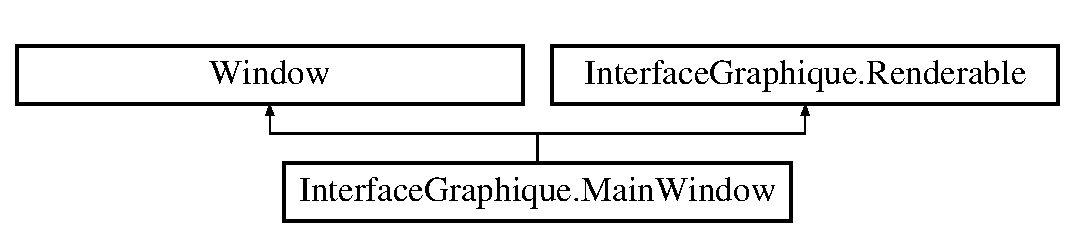
\includegraphics[height=2.000000cm]{class_interface_graphique_1_1_main_window}
\end{center}
\end{figure}
\subsection*{Public Member Functions}
\begin{DoxyCompactItemize}
\item 
\hypertarget{class_interface_graphique_1_1_main_window_af11d0f6c1d6519e421d5704f6a19c934}{}void {\bfseries Frame\+Update} (double time)\label{class_interface_graphique_1_1_main_window_af11d0f6c1d6519e421d5704f6a19c934}

\end{DoxyCompactItemize}


\subsection{Detailed Description}
Interaction logic for Main\+Window.\+xaml 



The documentation for this class was generated from the following file\+:\begin{DoxyCompactItemize}
\item 
Sources/\+Interface\+Graphique/Main\+Window.\+xaml.\+cs\end{DoxyCompactItemize}

\hypertarget{structmodele_1_1_materiau}{}\section{modele\+:\+:Materiau Struct Reference}
\label{structmodele_1_1_materiau}\index{modele\+::\+Materiau@{modele\+::\+Materiau}}


Structure comprennant les divers composants d\textquotesingle{}un matériau.  




{\ttfamily \#include $<$Materiau.\+h$>$}

\subsection*{Public Types}
\begin{DoxyCompactItemize}
\item 
\hypertarget{structmodele_1_1_materiau_a78b750424a82862ce601e47045027a88}{}using \hyperlink{structmodele_1_1_materiau_a78b750424a82862ce601e47045027a88}{Vec\+Type} = glm\+::vec3\label{structmodele_1_1_materiau_a78b750424a82862ce601e47045027a88}

\begin{DoxyCompactList}\small\item\em Alias de type. \end{DoxyCompactList}\end{DoxyCompactItemize}
\subsection*{Public Member Functions}
\begin{DoxyCompactItemize}
\item 
\hyperlink{group__rendering_ga10d9cab94019fabdd02e8bfc85df772f}{Materiau} (ai\+Material const $\ast$material)
\begin{DoxyCompactList}\small\item\em Constructeur à partir d\textquotesingle{}un matériau assimp. \end{DoxyCompactList}\end{DoxyCompactItemize}
\subsection*{Public Attributes}
\begin{DoxyCompactItemize}
\item 
\hypertarget{structmodele_1_1_materiau_aba871dbcee8a619f50d65588d65f2cd8}{}std\+::string \hyperlink{structmodele_1_1_materiau_aba871dbcee8a619f50d65588d65f2cd8}{nom\+\_\+}\label{structmodele_1_1_materiau_aba871dbcee8a619f50d65588d65f2cd8}

\begin{DoxyCompactList}\small\item\em Nom du matériau. \end{DoxyCompactList}\item 
\hypertarget{structmodele_1_1_materiau_af9e1e292564939ef1531c75535c88414}{}\hyperlink{structmodele_1_1_materiau_a78b750424a82862ce601e47045027a88}{Vec\+Type} \hyperlink{structmodele_1_1_materiau_af9e1e292564939ef1531c75535c88414}{diffuse\+\_\+}\label{structmodele_1_1_materiau_af9e1e292564939ef1531c75535c88414}

\begin{DoxyCompactList}\small\item\em Composante diffuse. \end{DoxyCompactList}\item 
\hypertarget{structmodele_1_1_materiau_acf0804478c2afd2fac9b591fe1b0be02}{}\hyperlink{structmodele_1_1_materiau_a78b750424a82862ce601e47045027a88}{Vec\+Type} \hyperlink{structmodele_1_1_materiau_acf0804478c2afd2fac9b591fe1b0be02}{speculaire\+\_\+}\label{structmodele_1_1_materiau_acf0804478c2afd2fac9b591fe1b0be02}

\begin{DoxyCompactList}\small\item\em Composante spéculaire. \end{DoxyCompactList}\item 
\hypertarget{structmodele_1_1_materiau_a365057e8dc4cba8fa309161ac5a0695f}{}\hyperlink{structmodele_1_1_materiau_a78b750424a82862ce601e47045027a88}{Vec\+Type} \hyperlink{structmodele_1_1_materiau_a365057e8dc4cba8fa309161ac5a0695f}{ambiant\+\_\+}\label{structmodele_1_1_materiau_a365057e8dc4cba8fa309161ac5a0695f}

\begin{DoxyCompactList}\small\item\em Composante ambiante. \end{DoxyCompactList}\item 
\hypertarget{structmodele_1_1_materiau_aea8340e86a5da1aedb1b38644ee17628}{}\hyperlink{structmodele_1_1_materiau_a78b750424a82862ce601e47045027a88}{Vec\+Type} \hyperlink{structmodele_1_1_materiau_aea8340e86a5da1aedb1b38644ee17628}{emission\+\_\+}\label{structmodele_1_1_materiau_aea8340e86a5da1aedb1b38644ee17628}

\begin{DoxyCompactList}\small\item\em Composante d\textquotesingle{}émission. \end{DoxyCompactList}\item 
\hypertarget{structmodele_1_1_materiau_af39730051e8be6a26638be94519f5752}{}\hyperlink{structmodele_1_1_materiau_a78b750424a82862ce601e47045027a88}{Vec\+Type} \hyperlink{structmodele_1_1_materiau_af39730051e8be6a26638be94519f5752}{transparence\+\_\+}\label{structmodele_1_1_materiau_af39730051e8be6a26638be94519f5752}

\begin{DoxyCompactList}\small\item\em Composante de transparence. \end{DoxyCompactList}\item 
\hypertarget{structmodele_1_1_materiau_a7f75f512c039d1b6216748d1fcd6385f}{}float \hyperlink{structmodele_1_1_materiau_a7f75f512c039d1b6216748d1fcd6385f}{opacite\+\_\+} \{ 0.\+0f \}\label{structmodele_1_1_materiau_a7f75f512c039d1b6216748d1fcd6385f}

\begin{DoxyCompactList}\small\item\em Composante d\textquotesingle{}opacité \end{DoxyCompactList}\item 
\hypertarget{structmodele_1_1_materiau_a2680f5328baae79f3108648ff2becf6c}{}float \hyperlink{structmodele_1_1_materiau_a2680f5328baae79f3108648ff2becf6c}{shininess\+\_\+} \{ 1.\+0f \}\label{structmodele_1_1_materiau_a2680f5328baae79f3108648ff2becf6c}

\begin{DoxyCompactList}\small\item\em Composante de brillance. \end{DoxyCompactList}\item 
\hypertarget{structmodele_1_1_materiau_a8f6f2673cf3489ea9fc88ce4358c8f0d}{}float \hyperlink{structmodele_1_1_materiau_a8f6f2673cf3489ea9fc88ce4358c8f0d}{shininess\+Strength\+\_\+} \{ 1.\+0f \}\label{structmodele_1_1_materiau_a8f6f2673cf3489ea9fc88ce4358c8f0d}

\begin{DoxyCompactList}\small\item\em Composante de force de brillance. \end{DoxyCompactList}\item 
\hypertarget{structmodele_1_1_materiau_a0c21796cf3ae0816ab2342d1c0524c27}{}std\+::string \hyperlink{structmodele_1_1_materiau_a0c21796cf3ae0816ab2342d1c0524c27}{nom\+Texture\+\_\+}\label{structmodele_1_1_materiau_a0c21796cf3ae0816ab2342d1c0524c27}

\begin{DoxyCompactList}\small\item\em Nom de la texture associée. \end{DoxyCompactList}\item 
\hypertarget{structmodele_1_1_materiau_a55e6d3d19eb038d86097568353cbad06}{}bool \hyperlink{structmodele_1_1_materiau_a55e6d3d19eb038d86097568353cbad06}{fil\+De\+Fer\+\_\+} \{ false \}\label{structmodele_1_1_materiau_a55e6d3d19eb038d86097568353cbad06}

\begin{DoxyCompactList}\small\item\em Mode de rendu (wireframe) \end{DoxyCompactList}\item 
\hypertarget{structmodele_1_1_materiau_aab5dc5905e9d580acdeba0bcc7853108}{}bool \hyperlink{structmodele_1_1_materiau_aab5dc5905e9d580acdeba0bcc7853108}{afficher\+Deux\+Cotes\+\_\+} \{ false \}\label{structmodele_1_1_materiau_aab5dc5905e9d580acdeba0bcc7853108}

\begin{DoxyCompactList}\small\item\em mode de culling (two-\/side) \end{DoxyCompactList}\end{DoxyCompactItemize}


\subsection{Detailed Description}
Structure comprennant les divers composants d\textquotesingle{}un matériau. 

\begin{DoxyAuthor}{Author}
Martin Paradis 
\end{DoxyAuthor}
\begin{DoxyDate}{Date}
2014-\/08-\/16 
\end{DoxyDate}


The documentation for this struct was generated from the following files\+:\begin{DoxyCompactItemize}
\item 
Commun/\+Utilitaire/\+Modele/\hyperlink{_materiau_8h}{Materiau.\+h}\item 
Commun/\+Utilitaire/\+Modele/\hyperlink{_materiau_8cpp}{Materiau.\+cpp}\end{DoxyCompactItemize}

\hypertarget{classmodele_1_1_mesh}{}\section{modele\+:\+:Mesh Class Reference}
\label{classmodele_1_1_mesh}\index{modele\+::\+Mesh@{modele\+::\+Mesh}}


Classe qui encapsule les données géométriques d\textquotesingle{}un modèle 3\+D, donc les vertices, les normales, les coordonnées de texture, les couleurs des vertices et les faces.  




{\ttfamily \#include $<$Mesh.\+h$>$}

\subsection*{Public Types}
\begin{DoxyCompactItemize}
\item 
\hypertarget{classmodele_1_1_mesh_adbc8897d8cdca4541a2068c874aa54eb}{}{\footnotesize template$<$typename T $>$ }\\using \hyperlink{classmodele_1_1_mesh_adbc8897d8cdca4541a2068c874aa54eb}{Conteneur} = std\+::vector$<$ T $>$\label{classmodele_1_1_mesh_adbc8897d8cdca4541a2068c874aa54eb}

\begin{DoxyCompactList}\small\item\em Alias de type. \end{DoxyCompactList}\item 
\hypertarget{classmodele_1_1_mesh_afff0dcaf39cb8aac23e07704fd404b92}{}using {\bfseries Vertex} = glm\+::vec3\label{classmodele_1_1_mesh_afff0dcaf39cb8aac23e07704fd404b92}

\item 
\hypertarget{classmodele_1_1_mesh_a3d99d2b7a917cf9366fcda290afed7e8}{}using {\bfseries Normale} = glm\+::vec3\label{classmodele_1_1_mesh_a3d99d2b7a917cf9366fcda290afed7e8}

\item 
\hypertarget{classmodele_1_1_mesh_a92ca30b14afcb78679c812e44cdf176d}{}using {\bfseries Tex\+Coord} = glm\+::vec2\label{classmodele_1_1_mesh_a92ca30b14afcb78679c812e44cdf176d}

\item 
\hypertarget{classmodele_1_1_mesh_a41e1ae261228cf93233b09232d6be11d}{}using {\bfseries Couleur} = glm\+::vec4\label{classmodele_1_1_mesh_a41e1ae261228cf93233b09232d6be11d}

\item 
\hypertarget{classmodele_1_1_mesh_a6977203afc00e8f371f49c91f7fab183}{}using {\bfseries Face} = glm\+::ivec3\label{classmodele_1_1_mesh_a6977203afc00e8f371f49c91f7fab183}

\end{DoxyCompactItemize}
\subsection*{Public Member Functions}
\begin{DoxyCompactItemize}
\item 
\hyperlink{classmodele_1_1_mesh_a37bac341d514cb2edf8c409d0ee5f7f8}{Mesh} (ai\+Scene const $\ast$scene, ai\+Mesh const $\ast$mesh)
\begin{DoxyCompactList}\small\item\em Constructeur à partir d\textquotesingle{}un mesh et d\textquotesingle{}une scène assimp. \end{DoxyCompactList}\item 
\hyperlink{classmodele_1_1_mesh_adbc8897d8cdca4541a2068c874aa54eb}{Conteneur}$<$ Vertex $>$ const \& \hyperlink{classmodele_1_1_mesh_acd81c408cf6963ff4605658cdc45b290}{obtenir\+Sommets} () const 
\begin{DoxyCompactList}\small\item\em Méthode pour obtenir les vertex du mesh. \end{DoxyCompactList}\item 
\hyperlink{classmodele_1_1_mesh_adbc8897d8cdca4541a2068c874aa54eb}{Conteneur}$<$ Normale $>$ const \& \hyperlink{classmodele_1_1_mesh_a88016a49bdd88d70afef9e590c7c4a11}{obtenir\+Normales} () const 
\begin{DoxyCompactList}\small\item\em Méthode pour obtenir les normales du mesh. \end{DoxyCompactList}\item 
\hyperlink{classmodele_1_1_mesh_adbc8897d8cdca4541a2068c874aa54eb}{Conteneur}$<$ Tex\+Coord $>$ const \& \hyperlink{classmodele_1_1_mesh_ac48a1ff182f6b68069b72eff692f8196}{obtenir\+Tex\+Coords} () const 
\begin{DoxyCompactList}\small\item\em Méthode pour obtenir les coordonnées de texture du mesh. \end{DoxyCompactList}\item 
\hyperlink{classmodele_1_1_mesh_adbc8897d8cdca4541a2068c874aa54eb}{Conteneur}$<$ Couleur $>$ const \& \hyperlink{classmodele_1_1_mesh_a4333bdb21580f548ef22bb3954b7c179}{obtenir\+Couleurs} () const 
\begin{DoxyCompactList}\small\item\em Méthode pour obtenir les couleurs des sommets du mesh. \end{DoxyCompactList}\item 
\hyperlink{structmodele_1_1_materiau}{Materiau} const \& \hyperlink{classmodele_1_1_mesh_ae072a8706a2a057780de35b4fbed1d19}{obtenir\+Materiau} () const 
\begin{DoxyCompactList}\small\item\em Méthode pour obtenir le materiau du mesh. \end{DoxyCompactList}\item 
\hyperlink{classmodele_1_1_mesh_adbc8897d8cdca4541a2068c874aa54eb}{Conteneur}$<$ Face $>$ const \& \hyperlink{classmodele_1_1_mesh_afd06495e1e6d7e870baf7e20b7862b8d}{obtenir\+Faces} () const 
\begin{DoxyCompactList}\small\item\em Méthode pour obtenir les couleurs des sommets du mesh. \end{DoxyCompactList}\item 
std\+::string const \& \hyperlink{classmodele_1_1_mesh_ad04c281e59a74438cd0f6564743c537b}{obtenir\+Nom} () const 
\begin{DoxyCompactList}\small\item\em Méthode pour obtenir le nom du noeud (souvent une chaine vide) \end{DoxyCompactList}\item 
bool \hyperlink{classmodele_1_1_mesh_aa7ff98102f4e390cd15df6d919474ff8}{possede\+Sommets} () const 
\begin{DoxyCompactList}\small\item\em Vérifier si le mesh contient des sommets. \end{DoxyCompactList}\item 
bool \hyperlink{classmodele_1_1_mesh_aca6001ed3c4bd55f854a442e97ac5258}{possede\+Normales} () const 
\begin{DoxyCompactList}\small\item\em Vérifier si le mesh contient des normales. \end{DoxyCompactList}\item 
bool \hyperlink{classmodele_1_1_mesh_a0ed3db0114de7a7674f252a78b35cad8}{possede\+Tex\+Coords} () const 
\begin{DoxyCompactList}\small\item\em Vérifier si le mesh contient des coordonnées de texture. \end{DoxyCompactList}\item 
bool \hyperlink{classmodele_1_1_mesh_a3655f655ce525b4d7448050a2f6692af}{possede\+Couleurs} () const 
\begin{DoxyCompactList}\small\item\em Vérifier si le mesh contient des couleurs de vertex. \end{DoxyCompactList}\item 
bool \hyperlink{classmodele_1_1_mesh_a542042fa090ce91d6d1858c1be91c5b4}{possede\+Faces} () const 
\begin{DoxyCompactList}\small\item\em Vérifier si le mesh contient des faces. \end{DoxyCompactList}\end{DoxyCompactItemize}


\subsection{Detailed Description}
Classe qui encapsule les données géométriques d\textquotesingle{}un modèle 3\+D, donc les vertices, les normales, les coordonnées de texture, les couleurs des vertices et les faces. 

\begin{DoxyAuthor}{Author}
Martin Paradis 
\end{DoxyAuthor}
\begin{DoxyDate}{Date}
2014-\/08-\/16 
\end{DoxyDate}


\subsection{Constructor \& Destructor Documentation}
\hypertarget{classmodele_1_1_mesh_a37bac341d514cb2edf8c409d0ee5f7f8}{}\index{modele\+::\+Mesh@{modele\+::\+Mesh}!Mesh@{Mesh}}
\index{Mesh@{Mesh}!modele\+::\+Mesh@{modele\+::\+Mesh}}
\subsubsection[{Mesh(ai\+Scene const $\ast$scene, ai\+Mesh const $\ast$mesh)}]{\setlength{\rightskip}{0pt plus 5cm}modele\+::\+Mesh\+::\+Mesh (
\begin{DoxyParamCaption}
\item[{ai\+Scene const $\ast$}]{scene, }
\item[{ai\+Mesh const $\ast$}]{mesh}
\end{DoxyParamCaption}
)}\label{classmodele_1_1_mesh_a37bac341d514cb2edf8c409d0ee5f7f8}


Constructeur à partir d\textquotesingle{}un mesh et d\textquotesingle{}une scène assimp. 

Construit un mesh à partir d\textquotesingle{}une scène et d\textquotesingle{}un mesh Assimp


\begin{DoxyParams}[1]{Parameters}
\mbox{\tt in}  & {\em scene} & \+: la scène contenant le modèle \\
\hline
\mbox{\tt in}  & {\em mesh} & \+: le mesh à importer\\
\hline
\end{DoxyParams}
\begin{DoxyReturn}{Returns}
Aucune. 
\end{DoxyReturn}
Le mesh contient les informations sur le nombre de données à importer, on réserve donc la mémoire pour éviter la réallocation.

Pour tous les sommets

Positions

Normales

Une seule texture 2\+D est supportée

Une seule couleur par vertex est supportée

Pour chaque face

Récupérer les indices de face

Assigner le materiau 

\subsection{Member Function Documentation}
\hypertarget{classmodele_1_1_mesh_a4333bdb21580f548ef22bb3954b7c179}{}\index{modele\+::\+Mesh@{modele\+::\+Mesh}!obtenir\+Couleurs@{obtenir\+Couleurs}}
\index{obtenir\+Couleurs@{obtenir\+Couleurs}!modele\+::\+Mesh@{modele\+::\+Mesh}}
\subsubsection[{obtenir\+Couleurs() const }]{\setlength{\rightskip}{0pt plus 5cm}{\bf Mesh\+::\+Conteneur}$<$ Mesh\+::\+Couleur $>$ const \& modele\+::\+Mesh\+::obtenir\+Couleurs (
\begin{DoxyParamCaption}
{}
\end{DoxyParamCaption}
) const\hspace{0.3cm}{\ttfamily [inline]}}\label{classmodele_1_1_mesh_a4333bdb21580f548ef22bb3954b7c179}


Méthode pour obtenir les couleurs des sommets du mesh. 

Cette fonction retourne les couleurs dont est composé le mesh.

\begin{DoxyReturn}{Returns}
les couleurs (const). 
\end{DoxyReturn}
\hypertarget{classmodele_1_1_mesh_afd06495e1e6d7e870baf7e20b7862b8d}{}\index{modele\+::\+Mesh@{modele\+::\+Mesh}!obtenir\+Faces@{obtenir\+Faces}}
\index{obtenir\+Faces@{obtenir\+Faces}!modele\+::\+Mesh@{modele\+::\+Mesh}}
\subsubsection[{obtenir\+Faces() const }]{\setlength{\rightskip}{0pt plus 5cm}{\bf Mesh\+::\+Conteneur}$<$ Mesh\+::\+Face $>$ const \& modele\+::\+Mesh\+::obtenir\+Faces (
\begin{DoxyParamCaption}
{}
\end{DoxyParamCaption}
) const\hspace{0.3cm}{\ttfamily [inline]}}\label{classmodele_1_1_mesh_afd06495e1e6d7e870baf7e20b7862b8d}


Méthode pour obtenir les couleurs des sommets du mesh. 

Cette fonction retourne les index des faces dont est composé le mesh. Les faces sont supposées toujours être des triangles.

\begin{DoxyReturn}{Returns}
les faces (const). 
\end{DoxyReturn}
\hypertarget{classmodele_1_1_mesh_ae072a8706a2a057780de35b4fbed1d19}{}\index{modele\+::\+Mesh@{modele\+::\+Mesh}!obtenir\+Materiau@{obtenir\+Materiau}}
\index{obtenir\+Materiau@{obtenir\+Materiau}!modele\+::\+Mesh@{modele\+::\+Mesh}}
\subsubsection[{obtenir\+Materiau() const }]{\setlength{\rightskip}{0pt plus 5cm}{\bf Materiau} const \& modele\+::\+Mesh\+::obtenir\+Materiau (
\begin{DoxyParamCaption}
{}
\end{DoxyParamCaption}
) const\hspace{0.3cm}{\ttfamily [inline]}}\label{classmodele_1_1_mesh_ae072a8706a2a057780de35b4fbed1d19}


Méthode pour obtenir le materiau du mesh. 

Cette fonction retourne le matériau dont est composé le mesh.

\begin{DoxyReturn}{Returns}
le materiau (const). 
\end{DoxyReturn}
\hypertarget{classmodele_1_1_mesh_ad04c281e59a74438cd0f6564743c537b}{}\index{modele\+::\+Mesh@{modele\+::\+Mesh}!obtenir\+Nom@{obtenir\+Nom}}
\index{obtenir\+Nom@{obtenir\+Nom}!modele\+::\+Mesh@{modele\+::\+Mesh}}
\subsubsection[{obtenir\+Nom() const }]{\setlength{\rightskip}{0pt plus 5cm}std\+::string const \& modele\+::\+Mesh\+::obtenir\+Nom (
\begin{DoxyParamCaption}
{}
\end{DoxyParamCaption}
) const\hspace{0.3cm}{\ttfamily [inline]}}\label{classmodele_1_1_mesh_ad04c281e59a74438cd0f6564743c537b}


Méthode pour obtenir le nom du noeud (souvent une chaine vide) 

Cette fonction retourne le nom du mesh courant. Le nom des meshes est très souvent vide (cela dépend du type de fichier utilisé).

\begin{DoxyReturn}{Returns}
Le nom du mesh (const). 
\end{DoxyReturn}
\hypertarget{classmodele_1_1_mesh_a88016a49bdd88d70afef9e590c7c4a11}{}\index{modele\+::\+Mesh@{modele\+::\+Mesh}!obtenir\+Normales@{obtenir\+Normales}}
\index{obtenir\+Normales@{obtenir\+Normales}!modele\+::\+Mesh@{modele\+::\+Mesh}}
\subsubsection[{obtenir\+Normales() const }]{\setlength{\rightskip}{0pt plus 5cm}{\bf Mesh\+::\+Conteneur}$<$ Mesh\+::\+Normale $>$ const \& modele\+::\+Mesh\+::obtenir\+Normales (
\begin{DoxyParamCaption}
{}
\end{DoxyParamCaption}
) const\hspace{0.3cm}{\ttfamily [inline]}}\label{classmodele_1_1_mesh_a88016a49bdd88d70afef9e590c7c4a11}


Méthode pour obtenir les normales du mesh. 

Cette fonction retourne les normales contenues dans le mesh.

\begin{DoxyReturn}{Returns}
les normales (const). 
\end{DoxyReturn}
\hypertarget{classmodele_1_1_mesh_acd81c408cf6963ff4605658cdc45b290}{}\index{modele\+::\+Mesh@{modele\+::\+Mesh}!obtenir\+Sommets@{obtenir\+Sommets}}
\index{obtenir\+Sommets@{obtenir\+Sommets}!modele\+::\+Mesh@{modele\+::\+Mesh}}
\subsubsection[{obtenir\+Sommets() const }]{\setlength{\rightskip}{0pt plus 5cm}{\bf Mesh\+::\+Conteneur}$<$ Mesh\+::\+Vertex $>$ const \& modele\+::\+Mesh\+::obtenir\+Sommets (
\begin{DoxyParamCaption}
{}
\end{DoxyParamCaption}
) const\hspace{0.3cm}{\ttfamily [inline]}}\label{classmodele_1_1_mesh_acd81c408cf6963ff4605658cdc45b290}


Méthode pour obtenir les vertex du mesh. 

Cette fonction retourne les sommets dont est composé le mesh.

\begin{DoxyReturn}{Returns}
les sommets (const). 
\end{DoxyReturn}
\hypertarget{classmodele_1_1_mesh_ac48a1ff182f6b68069b72eff692f8196}{}\index{modele\+::\+Mesh@{modele\+::\+Mesh}!obtenir\+Tex\+Coords@{obtenir\+Tex\+Coords}}
\index{obtenir\+Tex\+Coords@{obtenir\+Tex\+Coords}!modele\+::\+Mesh@{modele\+::\+Mesh}}
\subsubsection[{obtenir\+Tex\+Coords() const }]{\setlength{\rightskip}{0pt plus 5cm}{\bf Mesh\+::\+Conteneur}$<$ Mesh\+::\+Tex\+Coord $>$ const \& modele\+::\+Mesh\+::obtenir\+Tex\+Coords (
\begin{DoxyParamCaption}
{}
\end{DoxyParamCaption}
) const\hspace{0.3cm}{\ttfamily [inline]}}\label{classmodele_1_1_mesh_ac48a1ff182f6b68069b72eff692f8196}


Méthode pour obtenir les coordonnées de texture du mesh. 

Cette fonction retourne les coordonnées de texture dont est composé le mesh.

\begin{DoxyReturn}{Returns}
les coordonnées de textures (const). 
\end{DoxyReturn}
\hypertarget{classmodele_1_1_mesh_a3655f655ce525b4d7448050a2f6692af}{}\index{modele\+::\+Mesh@{modele\+::\+Mesh}!possede\+Couleurs@{possede\+Couleurs}}
\index{possede\+Couleurs@{possede\+Couleurs}!modele\+::\+Mesh@{modele\+::\+Mesh}}
\subsubsection[{possede\+Couleurs() const }]{\setlength{\rightskip}{0pt plus 5cm}bool modele\+::\+Mesh\+::possede\+Couleurs (
\begin{DoxyParamCaption}
{}
\end{DoxyParamCaption}
) const\hspace{0.3cm}{\ttfamily [inline]}}\label{classmodele_1_1_mesh_a3655f655ce525b4d7448050a2f6692af}


Vérifier si le mesh contient des couleurs de vertex. 

Cette fonction indique si le mesh contient des couleurs de sommets.

\begin{DoxyReturn}{Returns}
vrai si le mesh possède des couleurs de sommets, faux sinon. 
\end{DoxyReturn}
\hypertarget{classmodele_1_1_mesh_a542042fa090ce91d6d1858c1be91c5b4}{}\index{modele\+::\+Mesh@{modele\+::\+Mesh}!possede\+Faces@{possede\+Faces}}
\index{possede\+Faces@{possede\+Faces}!modele\+::\+Mesh@{modele\+::\+Mesh}}
\subsubsection[{possede\+Faces() const }]{\setlength{\rightskip}{0pt plus 5cm}bool modele\+::\+Mesh\+::possede\+Faces (
\begin{DoxyParamCaption}
{}
\end{DoxyParamCaption}
) const\hspace{0.3cm}{\ttfamily [inline]}}\label{classmodele_1_1_mesh_a542042fa090ce91d6d1858c1be91c5b4}


Vérifier si le mesh contient des faces. 

Cette fonction indique si le mesh contient des faces.

\begin{DoxyReturn}{Returns}
vrai si le mesh possède des faces, faux sinon. 
\end{DoxyReturn}
\hypertarget{classmodele_1_1_mesh_aca6001ed3c4bd55f854a442e97ac5258}{}\index{modele\+::\+Mesh@{modele\+::\+Mesh}!possede\+Normales@{possede\+Normales}}
\index{possede\+Normales@{possede\+Normales}!modele\+::\+Mesh@{modele\+::\+Mesh}}
\subsubsection[{possede\+Normales() const }]{\setlength{\rightskip}{0pt plus 5cm}bool modele\+::\+Mesh\+::possede\+Normales (
\begin{DoxyParamCaption}
{}
\end{DoxyParamCaption}
) const\hspace{0.3cm}{\ttfamily [inline]}}\label{classmodele_1_1_mesh_aca6001ed3c4bd55f854a442e97ac5258}


Vérifier si le mesh contient des normales. 

Cette fonction indique si le mesh contient des normales.

\begin{DoxyReturn}{Returns}
vrai si le mesh possède des normales, faux sinon. 
\end{DoxyReturn}
\hypertarget{classmodele_1_1_mesh_aa7ff98102f4e390cd15df6d919474ff8}{}\index{modele\+::\+Mesh@{modele\+::\+Mesh}!possede\+Sommets@{possede\+Sommets}}
\index{possede\+Sommets@{possede\+Sommets}!modele\+::\+Mesh@{modele\+::\+Mesh}}
\subsubsection[{possede\+Sommets() const }]{\setlength{\rightskip}{0pt plus 5cm}bool modele\+::\+Mesh\+::possede\+Sommets (
\begin{DoxyParamCaption}
{}
\end{DoxyParamCaption}
) const\hspace{0.3cm}{\ttfamily [inline]}}\label{classmodele_1_1_mesh_aa7ff98102f4e390cd15df6d919474ff8}


Vérifier si le mesh contient des sommets. 

Cette fonction indique si le mesh contient des sommets.

\begin{DoxyReturn}{Returns}
vrai si le mesh possède des sommets, faux sinon. 
\end{DoxyReturn}
\hypertarget{classmodele_1_1_mesh_a0ed3db0114de7a7674f252a78b35cad8}{}\index{modele\+::\+Mesh@{modele\+::\+Mesh}!possede\+Tex\+Coords@{possede\+Tex\+Coords}}
\index{possede\+Tex\+Coords@{possede\+Tex\+Coords}!modele\+::\+Mesh@{modele\+::\+Mesh}}
\subsubsection[{possede\+Tex\+Coords() const }]{\setlength{\rightskip}{0pt plus 5cm}bool modele\+::\+Mesh\+::possede\+Tex\+Coords (
\begin{DoxyParamCaption}
{}
\end{DoxyParamCaption}
) const\hspace{0.3cm}{\ttfamily [inline]}}\label{classmodele_1_1_mesh_a0ed3db0114de7a7674f252a78b35cad8}


Vérifier si le mesh contient des coordonnées de texture. 

Cette fonction indique si le mesh contient des coordonnées de texture.

\begin{DoxyReturn}{Returns}
vrai si le mesh possède des coordonnées de texture, faux sinon. 
\end{DoxyReturn}


The documentation for this class was generated from the following files\+:\begin{DoxyCompactItemize}
\item 
C\+:/\+Users/\+Louis/workspace/inf2990-\/01/\+Commun/\+Utilitaire/\+Modele/\hyperlink{_mesh_8h}{Mesh.\+h}\item 
C\+:/\+Users/\+Louis/workspace/inf2990-\/01/\+Commun/\+Utilitaire/\+Modele/\hyperlink{_mesh_8cpp}{Mesh.\+cpp}\end{DoxyCompactItemize}

\hypertarget{struct_interface_graphique_1_1_program_1_1_fonctions_natives_1_1_message}{\section{Référence de la structure Interface\-Graphique.\-Program.\-Fonctions\-Natives.\-Message}
\label{struct_interface_graphique_1_1_program_1_1_fonctions_natives_1_1_message}\index{Interface\-Graphique.\-Program.\-Fonctions\-Natives.\-Message@{Interface\-Graphique.\-Program.\-Fonctions\-Natives.\-Message}}
}
\subsection*{Attributs publics}
\begin{DoxyCompactItemize}
\item 
\hypertarget{struct_interface_graphique_1_1_program_1_1_fonctions_natives_1_1_message_a79723506feb45f5c0d016e2c4d1322ed}{Int\-Ptr {\bfseries h\-Wnd}}\label{struct_interface_graphique_1_1_program_1_1_fonctions_natives_1_1_message_a79723506feb45f5c0d016e2c4d1322ed}

\item 
\hypertarget{struct_interface_graphique_1_1_program_1_1_fonctions_natives_1_1_message_a89e12a8f443b5c702f97d60bb89ea92d}{uint {\bfseries Msg}}\label{struct_interface_graphique_1_1_program_1_1_fonctions_natives_1_1_message_a89e12a8f443b5c702f97d60bb89ea92d}

\item 
\hypertarget{struct_interface_graphique_1_1_program_1_1_fonctions_natives_1_1_message_a69a29b0891227cbc5365ba450e36f0ce}{Int\-Ptr {\bfseries w\-Param}}\label{struct_interface_graphique_1_1_program_1_1_fonctions_natives_1_1_message_a69a29b0891227cbc5365ba450e36f0ce}

\item 
\hypertarget{struct_interface_graphique_1_1_program_1_1_fonctions_natives_1_1_message_a80b40861c5792897ce18ddeeda6cf269}{Int\-Ptr {\bfseries l\-Param}}\label{struct_interface_graphique_1_1_program_1_1_fonctions_natives_1_1_message_a80b40861c5792897ce18ddeeda6cf269}

\item 
\hypertarget{struct_interface_graphique_1_1_program_1_1_fonctions_natives_1_1_message_a35f8a6545e405ca37256b2f25e1d4265}{uint {\bfseries Time}}\label{struct_interface_graphique_1_1_program_1_1_fonctions_natives_1_1_message_a35f8a6545e405ca37256b2f25e1d4265}

\item 
\hypertarget{struct_interface_graphique_1_1_program_1_1_fonctions_natives_1_1_message_a55b388f7eb95f804564f1d68c30c2422}{System.\-Drawing.\-Point {\bfseries Point}}\label{struct_interface_graphique_1_1_program_1_1_fonctions_natives_1_1_message_a55b388f7eb95f804564f1d68c30c2422}

\end{DoxyCompactItemize}


La documentation de cette structure a été générée à partir du fichier suivant \-:\begin{DoxyCompactItemize}
\item 
C\-:/\-Users/saron/\-Documents/inf2990-\/01/\-Sources/\-Interface\-Graphique/Program.\-cs\end{DoxyCompactItemize}

\hypertarget{class_mini_search}{\section{Référence de la classe Mini\-Search}
\label{class_mini_search}\index{Mini\-Search@{Mini\-Search}}
}
Graphe d'héritage de Mini\-Search\-:\begin{figure}[H]
\begin{center}
\leavevmode
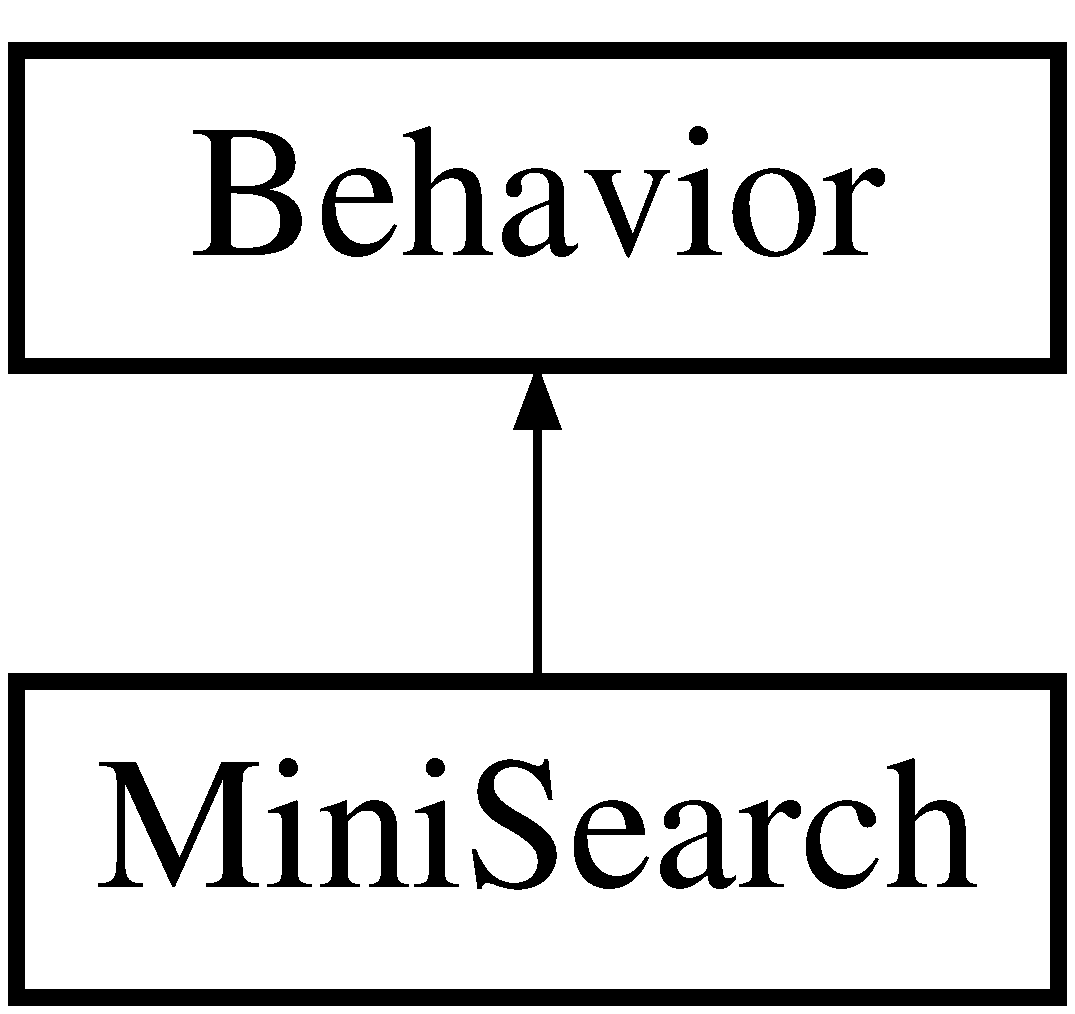
\includegraphics[height=2.000000cm]{class_mini_search}
\end{center}
\end{figure}
\subsection*{Fonctions membres publiques}
{\bf }\par
\begin{DoxyCompactItemize}
\item 
\hyperlink{class_mini_search_a24ade087d4c7e3afadae782ad0baa8da}{Mini\-Search} (\hyperlink{class_behavior_context}{Behavior\-Context} $\ast$context)
\begin{DoxyCompactList}\small\item\em Constructeur. \end{DoxyCompactList}\item 
void \hyperlink{class_mini_search_a307a770d20f6c9cd869d6e0853bb18ef}{do\-Action} () override
\begin{DoxyCompactList}\small\item\em Effectue une etape de son comportement. \end{DoxyCompactList}\end{DoxyCompactItemize}

\subsection*{Membres hérités additionnels}


\subsection{Documentation des constructeurs et destructeur}
\hypertarget{class_mini_search_a24ade087d4c7e3afadae782ad0baa8da}{\index{Mini\-Search@{Mini\-Search}!Mini\-Search@{Mini\-Search}}
\index{Mini\-Search@{Mini\-Search}!MiniSearch@{Mini\-Search}}
\subsubsection[{Mini\-Search}]{\setlength{\rightskip}{0pt plus 5cm}Mini\-Search\-::\-Mini\-Search (
\begin{DoxyParamCaption}
\item[{{\bf Behavior\-Context} $\ast$}]{context}
\end{DoxyParamCaption}
)}}\label{class_mini_search_a24ade087d4c7e3afadae782ad0baa8da}


Constructeur. 

Constructeur


\begin{DoxyParams}[1]{Paramètres}
\mbox{\tt in}  & {\em context} & \-: La classe pouvant accéder au robot.\\
\hline
\end{DoxyParams}
\begin{DoxyReturn}{Renvoie}
Aucune. 
\end{DoxyReturn}


\subsection{Documentation des fonctions membres}
\hypertarget{class_mini_search_a307a770d20f6c9cd869d6e0853bb18ef}{\index{Mini\-Search@{Mini\-Search}!do\-Action@{do\-Action}}
\index{do\-Action@{do\-Action}!MiniSearch@{Mini\-Search}}
\subsubsection[{do\-Action}]{\setlength{\rightskip}{0pt plus 5cm}void Mini\-Search\-::do\-Action (
\begin{DoxyParamCaption}
{}
\end{DoxyParamCaption}
)\hspace{0.3cm}{\ttfamily [override]}, {\ttfamily [virtual]}}}\label{class_mini_search_a307a770d20f6c9cd869d6e0853bb18ef}


Effectue une etape de son comportement. 

Cette fonction effectue le comportement de l'état actuel.


\begin{DoxyParams}[1]{Paramètres}
\mbox{\tt in}  & {\em Aucun.} & \\
\hline
\end{DoxyParams}
\begin{DoxyReturn}{Renvoie}
Aucune. 
\end{DoxyReturn}


Réimplémentée à partir de \hyperlink{group__inf2990_gac22f205bc85075ff707ad1f695c18439}{Behavior}.



La documentation de cette classe a été générée à partir des fichiers suivants \-:\begin{DoxyCompactItemize}
\item 
C\-:/\-Users/saron/\-Documents/inf2990-\/01/\-Sources/\-D\-L\-L/\-Behavior/\hyperlink{_mini_search_8h}{Mini\-Search.\-h}\item 
C\-:/\-Users/saron/\-Documents/inf2990-\/01/\-Sources/\-D\-L\-L/\-Behavior/\hyperlink{_mini_search_8cpp}{Mini\-Search.\-cpp}\end{DoxyCompactItemize}

\hypertarget{class_mini_search_final}{\section{Référence de la classe Mini\-Search\-Final}
\label{class_mini_search_final}\index{Mini\-Search\-Final@{Mini\-Search\-Final}}
}


Classe sous-\/etat pour l'etat \char`\"{}\-Follow\-Line\char`\"{}.  




{\ttfamily \#include $<$Mini\-Search\-Final.\-h$>$}

Graphe d'héritage de Mini\-Search\-Final\-:\begin{figure}[H]
\begin{center}
\leavevmode
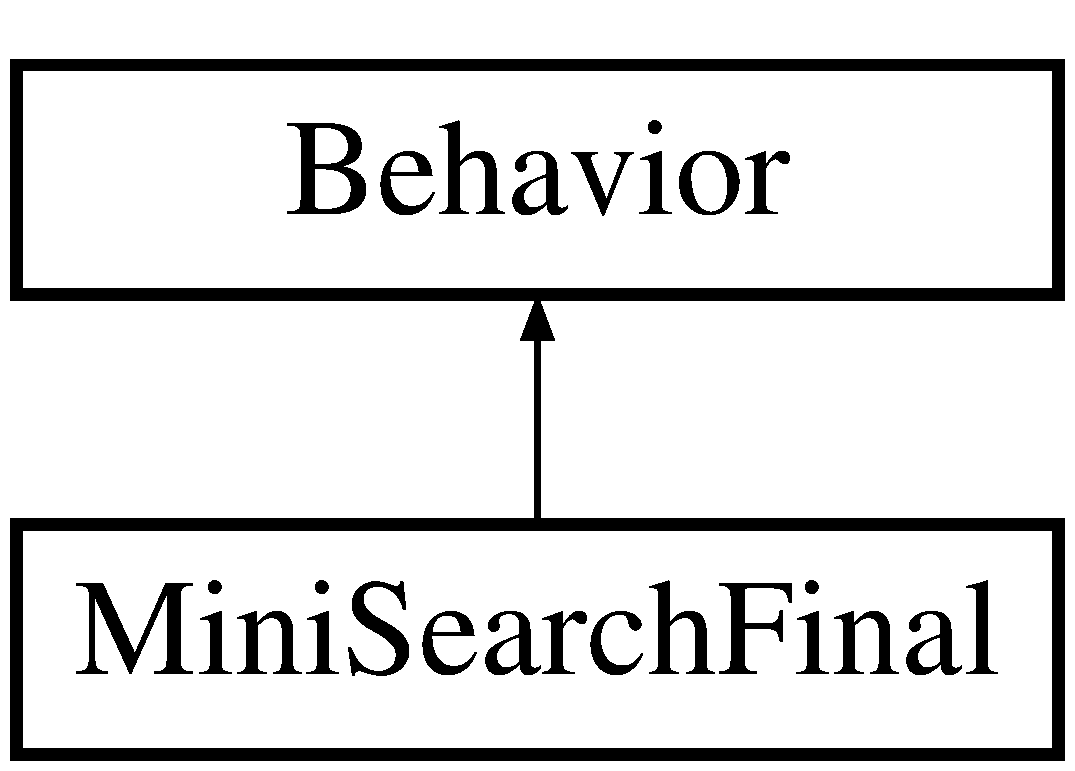
\includegraphics[height=2.000000cm]{class_mini_search_final}
\end{center}
\end{figure}
\subsection*{Fonctions membres publiques}
{\bf }\par
\begin{DoxyCompactItemize}
\item 
\hyperlink{class_mini_search_final_a8a16bd8a9e71bfefa9ffac6e5ca84505}{Mini\-Search\-Final} (\hyperlink{class_behavior_context}{Behavior\-Context} $\ast$context)
\begin{DoxyCompactList}\small\item\em Constructeur. \end{DoxyCompactList}\item 
void \hyperlink{class_mini_search_final_a1337f80dce8ad765072666fb9bcae9bc}{do\-Action} () override
\begin{DoxyCompactList}\small\item\em Effectue une etape de son comportement. \end{DoxyCompactList}\end{DoxyCompactItemize}

\subsection*{Membres hérités additionnels}


\subsection{Description détaillée}
Classe sous-\/etat pour l'etat \char`\"{}\-Follow\-Line\char`\"{}. 

\subsection{Documentation des constructeurs et destructeur}
\hypertarget{class_mini_search_final_a8a16bd8a9e71bfefa9ffac6e5ca84505}{\index{Mini\-Search\-Final@{Mini\-Search\-Final}!Mini\-Search\-Final@{Mini\-Search\-Final}}
\index{Mini\-Search\-Final@{Mini\-Search\-Final}!MiniSearchFinal@{Mini\-Search\-Final}}
\subsubsection[{Mini\-Search\-Final}]{\setlength{\rightskip}{0pt plus 5cm}Mini\-Search\-Final\-::\-Mini\-Search\-Final (
\begin{DoxyParamCaption}
\item[{{\bf Behavior\-Context} $\ast$}]{context}
\end{DoxyParamCaption}
)}}\label{class_mini_search_final_a8a16bd8a9e71bfefa9ffac6e5ca84505}


Constructeur. 

Constructeur


\begin{DoxyParams}[1]{Paramètres}
\mbox{\tt in}  & {\em context} & \-: La classe pouvant accéder au robot.\\
\hline
\end{DoxyParams}
\begin{DoxyReturn}{Renvoie}
Aucune. 
\end{DoxyReturn}


\subsection{Documentation des fonctions membres}
\hypertarget{class_mini_search_final_a1337f80dce8ad765072666fb9bcae9bc}{\index{Mini\-Search\-Final@{Mini\-Search\-Final}!do\-Action@{do\-Action}}
\index{do\-Action@{do\-Action}!MiniSearchFinal@{Mini\-Search\-Final}}
\subsubsection[{do\-Action}]{\setlength{\rightskip}{0pt plus 5cm}void Mini\-Search\-Final\-::do\-Action (
\begin{DoxyParamCaption}
{}
\end{DoxyParamCaption}
)\hspace{0.3cm}{\ttfamily [override]}, {\ttfamily [virtual]}}}\label{class_mini_search_final_a1337f80dce8ad765072666fb9bcae9bc}


Effectue une etape de son comportement. 

Cette fonction effectue le comportement de l'état actuel.


\begin{DoxyParams}[1]{Paramètres}
\mbox{\tt in}  & {\em Aucun.} & \\
\hline
\end{DoxyParams}
\begin{DoxyReturn}{Renvoie}
Aucune. 
\end{DoxyReturn}


Réimplémentée à partir de \hyperlink{group__inf2990_gac22f205bc85075ff707ad1f695c18439}{Behavior}.



La documentation de cette classe a été générée à partir des fichiers suivants \-:\begin{DoxyCompactItemize}
\item 
C\-:/\-Users/saron/\-Documents/inf2990-\/01/\-Sources/\-D\-L\-L/\-Behavior/\hyperlink{_mini_search_final_8h}{Mini\-Search\-Final.\-h}\item 
C\-:/\-Users/saron/\-Documents/inf2990-\/01/\-Sources/\-D\-L\-L/\-Behavior/\hyperlink{_mini_search_final_8cpp}{Mini\-Search\-Final.\-cpp}\end{DoxyCompactItemize}

\hypertarget{class_mini_search_line}{\section{Référence de la classe Mini\-Search\-Line}
\label{class_mini_search_line}\index{Mini\-Search\-Line@{Mini\-Search\-Line}}
}


Classe sous-\/etat pour l'etat \char`\"{}\-Follow\-Line\char`\"{}.  




{\ttfamily \#include $<$Mini\-Search.\-h$>$}



\subsection{Description détaillée}
Classe sous-\/etat pour l'etat \char`\"{}\-Follow\-Line\char`\"{}. 

La documentation de cette classe a été générée à partir du fichier suivant \-:\begin{DoxyCompactItemize}
\item 
C\-:/\-Users/saron/\-Documents/inf2990-\/01/\-Sources/\-D\-L\-L/\-Behavior/\hyperlink{_mini_search_8h}{Mini\-Search.\-h}\end{DoxyCompactItemize}

\hypertarget{class_mini_search_second}{\section{Référence de la classe Mini\-Search\-Second}
\label{class_mini_search_second}\index{Mini\-Search\-Second@{Mini\-Search\-Second}}
}


Classe sous-\/etat pour l'etat \char`\"{}\-Follow\-Line\char`\"{}.  




{\ttfamily \#include $<$Mini\-Search\-Second.\-h$>$}

Graphe d'héritage de Mini\-Search\-Second\-:\begin{figure}[H]
\begin{center}
\leavevmode
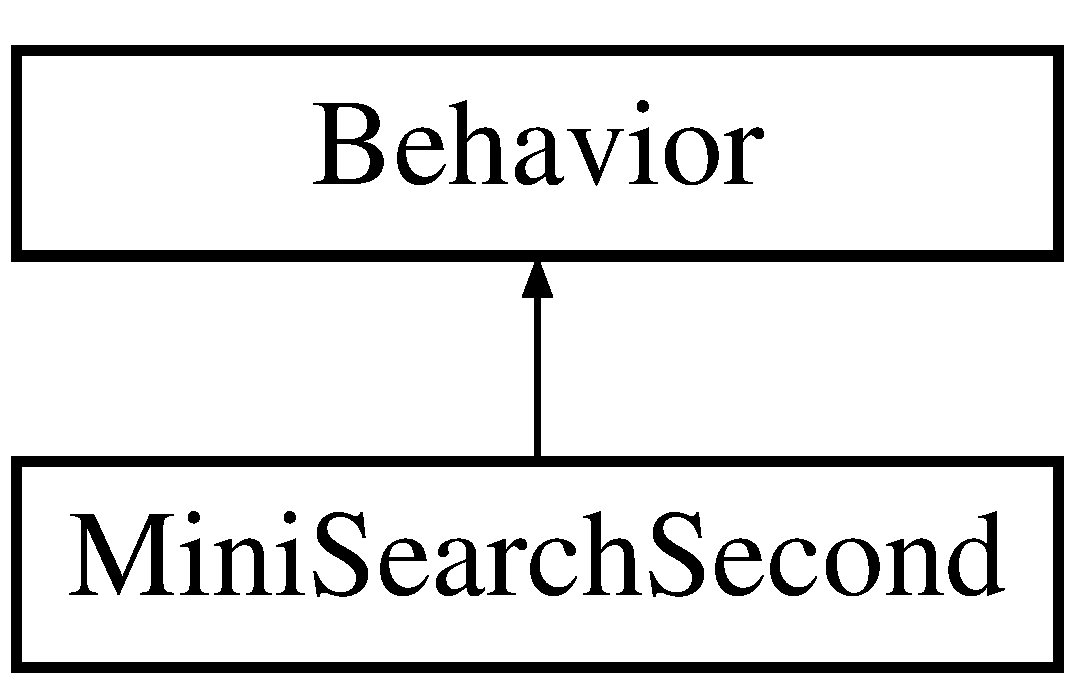
\includegraphics[height=2.000000cm]{class_mini_search_second}
\end{center}
\end{figure}
\subsection*{Fonctions membres publiques}
{\bf }\par
\begin{DoxyCompactItemize}
\item 
\hyperlink{class_mini_search_second_aa60f43e503ee0ad9b7806df496e12fc6}{Mini\-Search\-Second} (\hyperlink{class_behavior_context}{Behavior\-Context} $\ast$context)
\begin{DoxyCompactList}\small\item\em Constructeur. \end{DoxyCompactList}\item 
void \hyperlink{class_mini_search_second_aff8876aa2e43530ae1b10fb45579eeef}{do\-Action} () override
\begin{DoxyCompactList}\small\item\em Effectue une etape de son comportement. \end{DoxyCompactList}\end{DoxyCompactItemize}

\subsection*{Membres hérités additionnels}


\subsection{Description détaillée}
Classe sous-\/etat pour l'etat \char`\"{}\-Follow\-Line\char`\"{}. 

\subsection{Documentation des constructeurs et destructeur}
\hypertarget{class_mini_search_second_aa60f43e503ee0ad9b7806df496e12fc6}{\index{Mini\-Search\-Second@{Mini\-Search\-Second}!Mini\-Search\-Second@{Mini\-Search\-Second}}
\index{Mini\-Search\-Second@{Mini\-Search\-Second}!MiniSearchSecond@{Mini\-Search\-Second}}
\subsubsection[{Mini\-Search\-Second}]{\setlength{\rightskip}{0pt plus 5cm}Mini\-Search\-Second\-::\-Mini\-Search\-Second (
\begin{DoxyParamCaption}
\item[{{\bf Behavior\-Context} $\ast$}]{context}
\end{DoxyParamCaption}
)}}\label{class_mini_search_second_aa60f43e503ee0ad9b7806df496e12fc6}


Constructeur. 

Constructeur


\begin{DoxyParams}[1]{Paramètres}
\mbox{\tt in}  & {\em context} & \-: La classe pouvant accéder au robot.\\
\hline
\end{DoxyParams}
\begin{DoxyReturn}{Renvoie}
Aucune. 
\end{DoxyReturn}


\subsection{Documentation des fonctions membres}
\hypertarget{class_mini_search_second_aff8876aa2e43530ae1b10fb45579eeef}{\index{Mini\-Search\-Second@{Mini\-Search\-Second}!do\-Action@{do\-Action}}
\index{do\-Action@{do\-Action}!MiniSearchSecond@{Mini\-Search\-Second}}
\subsubsection[{do\-Action}]{\setlength{\rightskip}{0pt plus 5cm}void Mini\-Search\-Second\-::do\-Action (
\begin{DoxyParamCaption}
{}
\end{DoxyParamCaption}
)\hspace{0.3cm}{\ttfamily [override]}, {\ttfamily [virtual]}}}\label{class_mini_search_second_aff8876aa2e43530ae1b10fb45579eeef}


Effectue une etape de son comportement. 

Cette fonction effectue le comportement de l'état actuel.


\begin{DoxyParams}[1]{Paramètres}
\mbox{\tt in}  & {\em Aucun.} & \\
\hline
\end{DoxyParams}
\begin{DoxyReturn}{Renvoie}
Aucune. 
\end{DoxyReturn}


Réimplémentée à partir de \hyperlink{group__inf2990_gac22f205bc85075ff707ad1f695c18439}{Behavior}.



La documentation de cette classe a été générée à partir des fichiers suivants \-:\begin{DoxyCompactItemize}
\item 
C\-:/\-Users/saron/\-Documents/inf2990-\/01/\-Sources/\-D\-L\-L/\-Behavior/\hyperlink{_mini_search_second_8h}{Mini\-Search\-Second.\-h}\item 
C\-:/\-Users/saron/\-Documents/inf2990-\/01/\-Sources/\-D\-L\-L/\-Behavior/\hyperlink{_mini_search_second_8cpp}{Mini\-Search\-Second.\-cpp}\end{DoxyCompactItemize}

\hypertarget{classmodele_1_1_modele3_d}{\section{Référence de la classe modele\-:\-:Modele3\-D}
\label{classmodele_1_1_modele3_d}\index{modele\-::\-Modele3\-D@{modele\-::\-Modele3\-D}}
}


Classe qui encapsule un modèle 3d de la librairie 'assimp'. Cette classe permet de charger un modèle 3d d'un fichier exporté par un outil (en utilisant ladite librairie). La classe ne permet pas, dans sa forme actuelle, de modifier le modèle par la suite. Un point d'extension pourrait être de pouvoir animer le modèle en modifiant les matrices de transformation des noeuds contenant les meshes.  




{\ttfamily \#include $<$Modele3\-D.\-h$>$}

\subsection*{Types publics}
\begin{DoxyCompactItemize}
\item 
\hypertarget{classmodele_1_1_modele3_d_ab4241072ebd395ca1b9b6958ab8359cb}{using {\bfseries Path} = std\-::tr2\-::sys\-::path}\label{classmodele_1_1_modele3_d_ab4241072ebd395ca1b9b6958ab8359cb}

\end{DoxyCompactItemize}
\subsection*{Fonctions membres publiques}
\begin{DoxyCompactItemize}
\item 
\hyperlink{classmodele_1_1_modele3_d_a235e9fd8dddc14392f922fefaa11255a}{Modele3\-D} (\hyperlink{classmodele_1_1_modele3_d}{Modele3\-D} \&\&modele)
\begin{DoxyCompactList}\small\item\em Construction par transfert (\char`\"{}move\char`\"{}) \end{DoxyCompactList}\item 
\hyperlink{classmodele_1_1_modele3_d}{Modele3\-D} \& \hyperlink{classmodele_1_1_modele3_d_a34a330415e383970df2f479994f00dd6}{operator=} (\hyperlink{classmodele_1_1_modele3_d}{Modele3\-D} \&\&modele)
\begin{DoxyCompactList}\small\item\em Assignation par transfert (\char`\"{}move\char`\"{}) \end{DoxyCompactList}\item 
\hyperlink{classmodele_1_1_modele3_d_a1b028ca06d9bb0adda731be23de6d03b}{Modele3\-D} (\hyperlink{classmodele_1_1_modele3_d}{Modele3\-D} const \&)=delete
\item 
\hyperlink{classmodele_1_1_modele3_d}{Modele3\-D} \& \hyperlink{classmodele_1_1_modele3_d_af0336d4d17bb80b294b7b3d6212f94ba}{operator=} (\hyperlink{classmodele_1_1_modele3_d}{Modele3\-D} const \&)=delete
\item 
\hyperlink{classmodele_1_1_modele3_d_a1d3f1af73cee1aa3839dcd0eae9d1918}{$\sim$\-Modele3\-D} ()
\begin{DoxyCompactList}\small\item\em Destructeur. \end{DoxyCompactList}\item 
void \hyperlink{classmodele_1_1_modele3_d_aeb916b8eb492aef3aab86236773b81fb}{charger} (Path nom\-Fichier)
\begin{DoxyCompactList}\small\item\em Charger le modèle 3d à partir d'un fichier. \end{DoxyCompactList}\item 
bool \hyperlink{classmodele_1_1_modele3_d_a30920574e97a562609db9a2bde5df032}{possede\-Texture} (std\-::string const \&nom\-Texture) const 
\begin{DoxyCompactList}\small\item\em Permet de vérifier si la texture existe pour ce modèle. \end{DoxyCompactList}\item 
unsigned int \hyperlink{classmodele_1_1_modele3_d_a12d8fa87d7b2087866ea81af511041f4}{obtenir\-Texture\-Handle} (std\-::string const \&nom\-Texture) const 
\begin{DoxyCompactList}\small\item\em Pour permettre aux matériau de récupérer l'identifiant opengl de la texture. \end{DoxyCompactList}\item 
\hyperlink{classmodele_1_1_noeud}{Noeud} const \& \hyperlink{classmodele_1_1_modele3_d_af4d5e0bd8b91af3195086dda8fe019e3}{obtenir\-Noeud\-Racine} () const 
\begin{DoxyCompactList}\small\item\em Méthode d'obtention de l'arbre contenant les meshes. \end{DoxyCompactList}\item 
Path const \& \hyperlink{classmodele_1_1_modele3_d_ad175907ab5ce7898958ad42008db7869}{obtenir\-Chemin\-Fichier} () const 
\begin{DoxyCompactList}\small\item\em Méthode d'obtention du chemin du fichier chargé \end{DoxyCompactList}\end{DoxyCompactItemize}


\subsection{Description détaillée}
Classe qui encapsule un modèle 3d de la librairie 'assimp'. Cette classe permet de charger un modèle 3d d'un fichier exporté par un outil (en utilisant ladite librairie). La classe ne permet pas, dans sa forme actuelle, de modifier le modèle par la suite. Un point d'extension pourrait être de pouvoir animer le modèle en modifiant les matrices de transformation des noeuds contenant les meshes. 

\begin{DoxyNote}{Note}
Le rendu du modèle 3d est une responsabilité externe à la classe, puisqu'Open\-G\-L offre plusieurs méthodes de chargement des données sur la carte graphique et de dessin.
\end{DoxyNote}
\begin{DoxyAuthor}{Auteur}
Martin Paradis 
\end{DoxyAuthor}
\begin{DoxyDate}{Date}
2014-\/08-\/16 
\end{DoxyDate}


\subsection{Documentation des constructeurs et destructeur}
\hypertarget{classmodele_1_1_modele3_d_a235e9fd8dddc14392f922fefaa11255a}{\index{modele\-::\-Modele3\-D@{modele\-::\-Modele3\-D}!Modele3\-D@{Modele3\-D}}
\index{Modele3\-D@{Modele3\-D}!modele::Modele3D@{modele\-::\-Modele3\-D}}
\subsubsection[{Modele3\-D}]{\setlength{\rightskip}{0pt plus 5cm}modele\-::\-Modele3\-D\-::\-Modele3\-D (
\begin{DoxyParamCaption}
\item[{{\bf Modele3\-D} \&\&}]{modele}
\end{DoxyParamCaption}
)}}\label{classmodele_1_1_modele3_d_a235e9fd8dddc14392f922fefaa11255a}


Construction par transfert (\char`\"{}move\char`\"{}) 

Constructeur \char`\"{}move\char`\"{}. Utilise l'assignation \char`\"{}move\char`\"{}.

\begin{DoxyReturn}{Renvoie}
Aucune. 
\end{DoxyReturn}
\hypertarget{classmodele_1_1_modele3_d_a1b028ca06d9bb0adda731be23de6d03b}{\index{modele\-::\-Modele3\-D@{modele\-::\-Modele3\-D}!Modele3\-D@{Modele3\-D}}
\index{Modele3\-D@{Modele3\-D}!modele::Modele3D@{modele\-::\-Modele3\-D}}
\subsubsection[{Modele3\-D}]{\setlength{\rightskip}{0pt plus 5cm}modele\-::\-Modele3\-D\-::\-Modele3\-D (
\begin{DoxyParamCaption}
\item[{{\bf Modele3\-D} const \&}]{}
\end{DoxyParamCaption}
)\hspace{0.3cm}{\ttfamily [delete]}}}\label{classmodele_1_1_modele3_d_a1b028ca06d9bb0adda731be23de6d03b}
Pas de copie, car les identifiants de texture seraient dupliqués et relâchés sur la destruction \hypertarget{classmodele_1_1_modele3_d_a1d3f1af73cee1aa3839dcd0eae9d1918}{\index{modele\-::\-Modele3\-D@{modele\-::\-Modele3\-D}!$\sim$\-Modele3\-D@{$\sim$\-Modele3\-D}}
\index{$\sim$\-Modele3\-D@{$\sim$\-Modele3\-D}!modele::Modele3D@{modele\-::\-Modele3\-D}}
\subsubsection[{$\sim$\-Modele3\-D}]{\setlength{\rightskip}{0pt plus 5cm}modele\-::\-Modele3\-D\-::$\sim$\-Modele3\-D (
\begin{DoxyParamCaption}
{}
\end{DoxyParamCaption}
)}}\label{classmodele_1_1_modele3_d_a1d3f1af73cee1aa3839dcd0eae9d1918}


Destructeur. 

Destructeur. Ne fait que libérer les données des textures.

\begin{DoxyReturn}{Renvoie}
Aucune. 
\end{DoxyReturn}


\subsection{Documentation des fonctions membres}
\hypertarget{classmodele_1_1_modele3_d_aeb916b8eb492aef3aab86236773b81fb}{\index{modele\-::\-Modele3\-D@{modele\-::\-Modele3\-D}!charger@{charger}}
\index{charger@{charger}!modele::Modele3D@{modele\-::\-Modele3\-D}}
\subsubsection[{charger}]{\setlength{\rightskip}{0pt plus 5cm}void modele\-::\-Modele3\-D\-::charger (
\begin{DoxyParamCaption}
\item[{Path}]{chemin\-Fichier}
\end{DoxyParamCaption}
)}}\label{classmodele_1_1_modele3_d_aeb916b8eb492aef3aab86236773b81fb}


Charger le modèle 3d à partir d'un fichier. 

Cette fonction charge un modèle 3\-D à partir d'un fichier supporté par la librairie 'assimp'. Les textures Open\-G\-L afférentes sont également chargées.


\begin{DoxyParams}[1]{Paramètres}
\mbox{\tt in}  & {\em nom\-Fichier} & \-: nom du fichier modèle (normalement .obj ou .dae)\\
\hline
\end{DoxyParams}
\begin{DoxyReturn}{Renvoie}
Aucune. 
\end{DoxyReturn}
Ne pas charger le même fichier inutilement

Ne pas conserver les identifiants de texture d'un ancien modèle

Lors de l'importation, ne pas conserver les lignes et les points.

Le flag ai\-Process\-\_\-\-Triangulate, inclus dans ai\-Process\-Preset\-\_\-\-Target\-Realtime\-\_\-\-Quality, fera en sorte que les mesh ne comporteront que des triangles.

Charger l'ensemble des textures contenues dans le modèle \-:

Chargement des données du modèle 3\-D \hypertarget{classmodele_1_1_modele3_d_ad175907ab5ce7898958ad42008db7869}{\index{modele\-::\-Modele3\-D@{modele\-::\-Modele3\-D}!obtenir\-Chemin\-Fichier@{obtenir\-Chemin\-Fichier}}
\index{obtenir\-Chemin\-Fichier@{obtenir\-Chemin\-Fichier}!modele::Modele3D@{modele\-::\-Modele3\-D}}
\subsubsection[{obtenir\-Chemin\-Fichier}]{\setlength{\rightskip}{0pt plus 5cm}Modele3\-D\-::\-Path const \& modele\-::\-Modele3\-D\-::obtenir\-Chemin\-Fichier (
\begin{DoxyParamCaption}
{}
\end{DoxyParamCaption}
) const\hspace{0.3cm}{\ttfamily [inline]}}}\label{classmodele_1_1_modele3_d_ad175907ab5ce7898958ad42008db7869}


Méthode d'obtention du chemin du fichier chargé 

Cette fonction permet de récupérer le chemin du fichier chargé.

\begin{DoxyReturn}{Renvoie}
Le chemin du fichier chargé. 
\end{DoxyReturn}
\hypertarget{classmodele_1_1_modele3_d_af4d5e0bd8b91af3195086dda8fe019e3}{\index{modele\-::\-Modele3\-D@{modele\-::\-Modele3\-D}!obtenir\-Noeud\-Racine@{obtenir\-Noeud\-Racine}}
\index{obtenir\-Noeud\-Racine@{obtenir\-Noeud\-Racine}!modele::Modele3D@{modele\-::\-Modele3\-D}}
\subsubsection[{obtenir\-Noeud\-Racine}]{\setlength{\rightskip}{0pt plus 5cm}{\bf Noeud} const \& modele\-::\-Modele3\-D\-::obtenir\-Noeud\-Racine (
\begin{DoxyParamCaption}
{}
\end{DoxyParamCaption}
) const\hspace{0.3cm}{\ttfamily [inline]}}}\label{classmodele_1_1_modele3_d_af4d5e0bd8b91af3195086dda8fe019e3}


Méthode d'obtention de l'arbre contenant les meshes. 

Cette fonction retourne le noeud racine de l'arbre contenant les meshes du modèle 3\-D.

\begin{DoxyReturn}{Renvoie}
Le noeud racine (const). 
\end{DoxyReturn}
\hypertarget{classmodele_1_1_modele3_d_a12d8fa87d7b2087866ea81af511041f4}{\index{modele\-::\-Modele3\-D@{modele\-::\-Modele3\-D}!obtenir\-Texture\-Handle@{obtenir\-Texture\-Handle}}
\index{obtenir\-Texture\-Handle@{obtenir\-Texture\-Handle}!modele::Modele3D@{modele\-::\-Modele3\-D}}
\subsubsection[{obtenir\-Texture\-Handle}]{\setlength{\rightskip}{0pt plus 5cm}unsigned int modele\-::\-Modele3\-D\-::obtenir\-Texture\-Handle (
\begin{DoxyParamCaption}
\item[{std\-::string const \&}]{nom\-Texture}
\end{DoxyParamCaption}
) const\hspace{0.3cm}{\ttfamily [inline]}}}\label{classmodele_1_1_modele3_d_a12d8fa87d7b2087866ea81af511041f4}


Pour permettre aux matériau de récupérer l'identifiant opengl de la texture. 

Cette fonction permet de récupérer l'identifiant opengl de la texture.


\begin{DoxyParams}[1]{Paramètres}
\mbox{\tt in}  & {\em nom\-Texture} & \-: le nom de la texture\\
\hline
\end{DoxyParams}
\begin{DoxyReturn}{Renvoie}
Le handle vers la texture. 
\end{DoxyReturn}
\hypertarget{classmodele_1_1_modele3_d_a34a330415e383970df2f479994f00dd6}{\index{modele\-::\-Modele3\-D@{modele\-::\-Modele3\-D}!operator=@{operator=}}
\index{operator=@{operator=}!modele::Modele3D@{modele\-::\-Modele3\-D}}
\subsubsection[{operator=}]{\setlength{\rightskip}{0pt plus 5cm}{\bf Modele3\-D} \& modele\-::\-Modele3\-D\-::operator= (
\begin{DoxyParamCaption}
\item[{{\bf Modele3\-D} \&\&}]{modele}
\end{DoxyParamCaption}
)}}\label{classmodele_1_1_modele3_d_a34a330415e383970df2f479994f00dd6}


Assignation par transfert (\char`\"{}move\char`\"{}) 

Assignation par transfert (\char`\"{}move\char`\"{}), ne fait que transférer les données et s'assurer que les textures Open\-G\-L ne seront pas libérées lors de la destruction du modèle passé en paramètre.

\begin{DoxyReturn}{Renvoie}
le modèle courant. 
\end{DoxyReturn}
\hypertarget{classmodele_1_1_modele3_d_af0336d4d17bb80b294b7b3d6212f94ba}{\index{modele\-::\-Modele3\-D@{modele\-::\-Modele3\-D}!operator=@{operator=}}
\index{operator=@{operator=}!modele::Modele3D@{modele\-::\-Modele3\-D}}
\subsubsection[{operator=}]{\setlength{\rightskip}{0pt plus 5cm}{\bf Modele3\-D}\& modele\-::\-Modele3\-D\-::operator= (
\begin{DoxyParamCaption}
\item[{{\bf Modele3\-D} const \&}]{}
\end{DoxyParamCaption}
)\hspace{0.3cm}{\ttfamily [delete]}}}\label{classmodele_1_1_modele3_d_af0336d4d17bb80b294b7b3d6212f94ba}
Pas d'assignation, car les identifiants de texture seraient dupliqués et relâchés sur la destruction \hypertarget{classmodele_1_1_modele3_d_a30920574e97a562609db9a2bde5df032}{\index{modele\-::\-Modele3\-D@{modele\-::\-Modele3\-D}!possede\-Texture@{possede\-Texture}}
\index{possede\-Texture@{possede\-Texture}!modele::Modele3D@{modele\-::\-Modele3\-D}}
\subsubsection[{possede\-Texture}]{\setlength{\rightskip}{0pt plus 5cm}bool modele\-::\-Modele3\-D\-::possede\-Texture (
\begin{DoxyParamCaption}
\item[{std\-::string const \&}]{nom\-Texture}
\end{DoxyParamCaption}
) const\hspace{0.3cm}{\ttfamily [inline]}}}\label{classmodele_1_1_modele3_d_a30920574e97a562609db9a2bde5df032}


Permet de vérifier si la texture existe pour ce modèle. 

Cette fonction permet de vérifier si la texture existe pour ce modèle


\begin{DoxyParams}[1]{Paramètres}
\mbox{\tt in}  & {\em nom\-Texture} & \-: le nom de la texture\\
\hline
\end{DoxyParams}
\begin{DoxyReturn}{Renvoie}
vrai si la texture est utilisée par le modèle, faux sinon. 
\end{DoxyReturn}


La documentation de cette classe a été générée à partir des fichiers suivants \-:\begin{DoxyCompactItemize}
\item 
C\-:/\-Users/saron/\-Documents/inf2990-\/01/\-Commun/\-Utilitaire/\-Modele/\hyperlink{_modele3_d_8h}{Modele3\-D.\-h}\item 
C\-:/\-Users/saron/\-Documents/inf2990-\/01/\-Commun/\-Utilitaire/\-Modele/\hyperlink{_modele3_d_8cpp}{Modele3\-D.\-cpp}\end{DoxyCompactItemize}

\hypertarget{class_interface_graphique_1_1_tools_1_1_move}{}\section{Interface\+Graphique.\+Tools.\+Move Class Reference}
\label{class_interface_graphique_1_1_tools_1_1_move}\index{Interface\+Graphique.\+Tools.\+Move@{Interface\+Graphique.\+Tools.\+Move}}


Représente l\textquotesingle{}outil de déplacement.  


Inheritance diagram for Interface\+Graphique.\+Tools.\+Move\+:\begin{figure}[H]
\begin{center}
\leavevmode
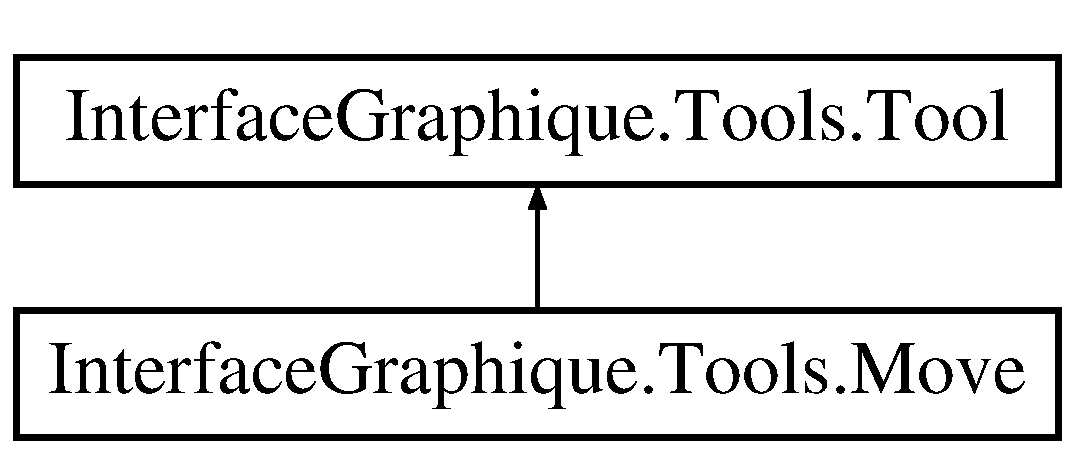
\includegraphics[height=2.000000cm]{class_interface_graphique_1_1_tools_1_1_move}
\end{center}
\end{figure}
\subsection*{Public Member Functions}
\begin{DoxyCompactItemize}
\item 
\hypertarget{class_interface_graphique_1_1_tools_1_1_move_aa447ff931a7cb490a7b44de3a7589292}{}delegate void {\bfseries Node\+Changed\+Event\+Handler} ()\label{class_interface_graphique_1_1_tools_1_1_move_aa447ff931a7cb490a7b44de3a7589292}

\item 
\hypertarget{class_interface_graphique_1_1_tools_1_1_move_a3874341a9c03a104287546f92b72cea9}{}{\bfseries Move} (\hyperlink{class_interface_graphique_1_1_tools_1_1_tool_context}{Tool\+Context} context)\label{class_interface_graphique_1_1_tools_1_1_move_a3874341a9c03a104287546f92b72cea9}

\item 
override void \hyperlink{class_interface_graphique_1_1_tools_1_1_move_a9bb3775998416ea36c2ca7009f37a6d9}{Left\+Mouse\+Pressed} (Mouse\+Event\+Args e)
\item 
override void \hyperlink{class_interface_graphique_1_1_tools_1_1_move_abff4c343d842c5513749a8c1f4c35338}{Left\+Mouse\+Released} (Mouse\+Event\+Args e)
\item 
override void \hyperlink{class_interface_graphique_1_1_tools_1_1_move_ab3c7919f138fa833fdf999adba7c8fdb}{Left\+Mouse\+Full\+Clicked} (Mouse\+Event\+Args e)
\item 
override void \hyperlink{class_interface_graphique_1_1_tools_1_1_move_ab6ce1689b59b7b60c55838ff344c8d7c}{Dragging} (int delta\+X, int delta\+Y, int delta\+Z)
\item 
override void \hyperlink{class_interface_graphique_1_1_tools_1_1_move_ab9f7749ef77fb21f385a9bc5b43bf234}{Mouse\+Move} (Mouse\+Event\+Args e)
\item 
override void \hyperlink{class_interface_graphique_1_1_tools_1_1_move_a72e41dcdef93cd060e499bd1f8683512}{esc} ()
\end{DoxyCompactItemize}
\subsection*{Events}
\begin{DoxyCompactItemize}
\item 
\hypertarget{class_interface_graphique_1_1_tools_1_1_move_a058bd0ebedbf308c53ef687bf07d8095}{}Node\+Changed\+Event\+Handler {\bfseries Node\+Changed\+Event}\label{class_interface_graphique_1_1_tools_1_1_move_a058bd0ebedbf308c53ef687bf07d8095}

\end{DoxyCompactItemize}


\subsection{Detailed Description}
Représente l\textquotesingle{}outil de déplacement. 

\begin{DoxyAuthor}{Author}
I\+N\+F2990-\/\+A15-\/01 
\end{DoxyAuthor}
\begin{DoxyDate}{Date}
2015-\/10-\/01 
\end{DoxyDate}


\subsection{Member Function Documentation}
\hypertarget{class_interface_graphique_1_1_tools_1_1_move_ab6ce1689b59b7b60c55838ff344c8d7c}{}\index{Interface\+Graphique\+::\+Tools\+::\+Move@{Interface\+Graphique\+::\+Tools\+::\+Move}!Dragging@{Dragging}}
\index{Dragging@{Dragging}!Interface\+Graphique\+::\+Tools\+::\+Move@{Interface\+Graphique\+::\+Tools\+::\+Move}}
\subsubsection[{Dragging(int delta\+X, int delta\+Y, int delta\+Z)}]{\setlength{\rightskip}{0pt plus 5cm}override void Interface\+Graphique.\+Tools.\+Move.\+Dragging (
\begin{DoxyParamCaption}
\item[{int}]{delta\+X, }
\item[{int}]{delta\+Y, }
\item[{int}]{delta\+Z}
\end{DoxyParamCaption}
)\hspace{0.3cm}{\ttfamily [inline]}, {\ttfamily [virtual]}}\label{class_interface_graphique_1_1_tools_1_1_move_ab6ce1689b59b7b60c55838ff344c8d7c}
Appelé dès qu\textquotesingle{}on bouge des éléments


\begin{DoxyParams}[1]{Parameters}
\mbox{\tt in}  & {\em delta\+X} & \+: la distance en X \\
\hline
\mbox{\tt in}  & {\em delta\+Y} & \+: la distance en Y \\
\hline
\mbox{\tt in}  & {\em delta\+Z} & \+: la distance en Z\\
\hline
\end{DoxyParams}
\begin{DoxyReturn}{Returns}
Aucun 
\end{DoxyReturn}


Reimplemented from \hyperlink{class_interface_graphique_1_1_tools_1_1_tool_a8b9595e6a3eb55443b8b2cdb38a2c390}{Interface\+Graphique.\+Tools.\+Tool}.

\hypertarget{class_interface_graphique_1_1_tools_1_1_move_a72e41dcdef93cd060e499bd1f8683512}{}\index{Interface\+Graphique\+::\+Tools\+::\+Move@{Interface\+Graphique\+::\+Tools\+::\+Move}!esc@{esc}}
\index{esc@{esc}!Interface\+Graphique\+::\+Tools\+::\+Move@{Interface\+Graphique\+::\+Tools\+::\+Move}}
\subsubsection[{esc()}]{\setlength{\rightskip}{0pt plus 5cm}override void Interface\+Graphique.\+Tools.\+Move.\+esc (
\begin{DoxyParamCaption}
{}
\end{DoxyParamCaption}
)\hspace{0.3cm}{\ttfamily [inline]}, {\ttfamily [virtual]}}\label{class_interface_graphique_1_1_tools_1_1_move_a72e41dcdef93cd060e499bd1f8683512}
Appelé quand on fait escape

\begin{DoxyReturn}{Returns}
Aucun 
\end{DoxyReturn}


Reimplemented from \hyperlink{class_interface_graphique_1_1_tools_1_1_tool_a734cc3904ce75149652ac356caba93f7}{Interface\+Graphique.\+Tools.\+Tool}.

\hypertarget{class_interface_graphique_1_1_tools_1_1_move_ab3c7919f138fa833fdf999adba7c8fdb}{}\index{Interface\+Graphique\+::\+Tools\+::\+Move@{Interface\+Graphique\+::\+Tools\+::\+Move}!Left\+Mouse\+Full\+Clicked@{Left\+Mouse\+Full\+Clicked}}
\index{Left\+Mouse\+Full\+Clicked@{Left\+Mouse\+Full\+Clicked}!Interface\+Graphique\+::\+Tools\+::\+Move@{Interface\+Graphique\+::\+Tools\+::\+Move}}
\subsubsection[{Left\+Mouse\+Full\+Clicked(\+Mouse\+Event\+Args e)}]{\setlength{\rightskip}{0pt plus 5cm}override void Interface\+Graphique.\+Tools.\+Move.\+Left\+Mouse\+Full\+Clicked (
\begin{DoxyParamCaption}
\item[{Mouse\+Event\+Args}]{e}
\end{DoxyParamCaption}
)\hspace{0.3cm}{\ttfamily [inline]}, {\ttfamily [virtual]}}\label{class_interface_graphique_1_1_tools_1_1_move_ab3c7919f138fa833fdf999adba7c8fdb}
Appelé quand on appuis et relâche sur le bouton gauche de la souris à l\textquotesingle{}intérieur de trois pixels. Représente un click.


\begin{DoxyParams}[1]{Parameters}
\mbox{\tt in}  & {\em e} & \+: les informations sur l\textquotesingle{}événement\\
\hline
\end{DoxyParams}
\begin{DoxyReturn}{Returns}
Aucun 
\end{DoxyReturn}


Reimplemented from \hyperlink{class_interface_graphique_1_1_tools_1_1_tool_a043f210d7840ec8aa5723b193e71ead5}{Interface\+Graphique.\+Tools.\+Tool}.

\hypertarget{class_interface_graphique_1_1_tools_1_1_move_a9bb3775998416ea36c2ca7009f37a6d9}{}\index{Interface\+Graphique\+::\+Tools\+::\+Move@{Interface\+Graphique\+::\+Tools\+::\+Move}!Left\+Mouse\+Pressed@{Left\+Mouse\+Pressed}}
\index{Left\+Mouse\+Pressed@{Left\+Mouse\+Pressed}!Interface\+Graphique\+::\+Tools\+::\+Move@{Interface\+Graphique\+::\+Tools\+::\+Move}}
\subsubsection[{Left\+Mouse\+Pressed(\+Mouse\+Event\+Args e)}]{\setlength{\rightskip}{0pt plus 5cm}override void Interface\+Graphique.\+Tools.\+Move.\+Left\+Mouse\+Pressed (
\begin{DoxyParamCaption}
\item[{Mouse\+Event\+Args}]{e}
\end{DoxyParamCaption}
)\hspace{0.3cm}{\ttfamily [inline]}, {\ttfamily [virtual]}}\label{class_interface_graphique_1_1_tools_1_1_move_a9bb3775998416ea36c2ca7009f37a6d9}
Appelé quand on appuis sur le bouton gauche de la souris


\begin{DoxyParams}[1]{Parameters}
\mbox{\tt in}  & {\em e} & \+: les informations sur l\textquotesingle{}événement\\
\hline
\end{DoxyParams}
\begin{DoxyReturn}{Returns}
Aucun 
\end{DoxyReturn}


Reimplemented from \hyperlink{class_interface_graphique_1_1_tools_1_1_tool_af5c8a4b2773f0d09f45575ade24769ba}{Interface\+Graphique.\+Tools.\+Tool}.

\hypertarget{class_interface_graphique_1_1_tools_1_1_move_abff4c343d842c5513749a8c1f4c35338}{}\index{Interface\+Graphique\+::\+Tools\+::\+Move@{Interface\+Graphique\+::\+Tools\+::\+Move}!Left\+Mouse\+Released@{Left\+Mouse\+Released}}
\index{Left\+Mouse\+Released@{Left\+Mouse\+Released}!Interface\+Graphique\+::\+Tools\+::\+Move@{Interface\+Graphique\+::\+Tools\+::\+Move}}
\subsubsection[{Left\+Mouse\+Released(\+Mouse\+Event\+Args e)}]{\setlength{\rightskip}{0pt plus 5cm}override void Interface\+Graphique.\+Tools.\+Move.\+Left\+Mouse\+Released (
\begin{DoxyParamCaption}
\item[{Mouse\+Event\+Args}]{e}
\end{DoxyParamCaption}
)\hspace{0.3cm}{\ttfamily [inline]}, {\ttfamily [virtual]}}\label{class_interface_graphique_1_1_tools_1_1_move_abff4c343d842c5513749a8c1f4c35338}
Appelé quand on relâche sur le bouton gauche de la souris


\begin{DoxyParams}[1]{Parameters}
\mbox{\tt in}  & {\em e} & \+: les informations sur l\textquotesingle{}événement\\
\hline
\end{DoxyParams}
\begin{DoxyReturn}{Returns}
Aucun 
\end{DoxyReturn}


Reimplemented from \hyperlink{class_interface_graphique_1_1_tools_1_1_tool_a51c4828f7d24c599b5748b9b3f64d39e}{Interface\+Graphique.\+Tools.\+Tool}.

\hypertarget{class_interface_graphique_1_1_tools_1_1_move_ab9f7749ef77fb21f385a9bc5b43bf234}{}\index{Interface\+Graphique\+::\+Tools\+::\+Move@{Interface\+Graphique\+::\+Tools\+::\+Move}!Mouse\+Move@{Mouse\+Move}}
\index{Mouse\+Move@{Mouse\+Move}!Interface\+Graphique\+::\+Tools\+::\+Move@{Interface\+Graphique\+::\+Tools\+::\+Move}}
\subsubsection[{Mouse\+Move(\+Mouse\+Event\+Args e)}]{\setlength{\rightskip}{0pt plus 5cm}override void Interface\+Graphique.\+Tools.\+Move.\+Mouse\+Move (
\begin{DoxyParamCaption}
\item[{Mouse\+Event\+Args}]{e}
\end{DoxyParamCaption}
)\hspace{0.3cm}{\ttfamily [inline]}, {\ttfamily [virtual]}}\label{class_interface_graphique_1_1_tools_1_1_move_ab9f7749ef77fb21f385a9bc5b43bf234}
Appelé quand on bouge la souris


\begin{DoxyParams}[1]{Parameters}
\mbox{\tt in}  & {\em e} & \+: les informations sur l\textquotesingle{}événement\\
\hline
\end{DoxyParams}
\begin{DoxyReturn}{Returns}
Aucun 
\end{DoxyReturn}


Reimplemented from \hyperlink{class_interface_graphique_1_1_tools_1_1_tool_aedd1c93f96ee602475b7cbc3c9c99baa}{Interface\+Graphique.\+Tools.\+Tool}.



The documentation for this class was generated from the following file\+:\begin{DoxyCompactItemize}
\item 
C\+:/\+Users/\+Louis/workspace/inf2990-\/01/\+Sources/\+Interface\+Graphique/\+Tools/Move.\+cs\end{DoxyCompactItemize}

\hypertarget{struct_interface_graphique_1_1_node_data}{\section{Référence de la structure Interface\-Graphique.\-Node\-Data}
\label{struct_interface_graphique_1_1_node_data}\index{Interface\-Graphique.\-Node\-Data@{Interface\-Graphique.\-Node\-Data}}
}
\subsection*{Attributs publics}
\begin{DoxyCompactItemize}
\item 
\hypertarget{struct_interface_graphique_1_1_node_data_aa65b000f8aca6ca4ef06867dece673bc}{float {\bfseries pos\-\_\-x}}\label{struct_interface_graphique_1_1_node_data_aa65b000f8aca6ca4ef06867dece673bc}

\item 
\hypertarget{struct_interface_graphique_1_1_node_data_a9f8a6932e2af21e5c9de9ca0da1b10d5}{float {\bfseries pos\-\_\-y}}\label{struct_interface_graphique_1_1_node_data_a9f8a6932e2af21e5c9de9ca0da1b10d5}

\item 
\hypertarget{struct_interface_graphique_1_1_node_data_af70290d20df57f31d3836eb0d43849f8}{float {\bfseries scale\-\_\-x}}\label{struct_interface_graphique_1_1_node_data_af70290d20df57f31d3836eb0d43849f8}

\item 
\hypertarget{struct_interface_graphique_1_1_node_data_a40c67aeb78481a26523814f70e839ddd}{float {\bfseries scale\-\_\-y}}\label{struct_interface_graphique_1_1_node_data_a40c67aeb78481a26523814f70e839ddd}

\item 
\hypertarget{struct_interface_graphique_1_1_node_data_a667c8cab7e202742610cb8ce22ad1e45}{float {\bfseries angle}}\label{struct_interface_graphique_1_1_node_data_a667c8cab7e202742610cb8ce22ad1e45}

\item 
\hypertarget{struct_interface_graphique_1_1_node_data_adf70f17797f2ab0d097d6462b959e823}{String {\bfseries type}}\label{struct_interface_graphique_1_1_node_data_adf70f17797f2ab0d097d6462b959e823}

\end{DoxyCompactItemize}


La documentation de cette structure a été générée à partir du fichier suivant \-:\begin{DoxyCompactItemize}
\item 
C\-:/\-Users/saron/\-Documents/inf2990-\/01/\-Sources/\-Interface\-Graphique/Editor.\-xaml.\-cs\end{DoxyCompactItemize}

\hypertarget{struct_node_properties}{}\section{Node\+Properties Struct Reference}
\label{struct_node_properties}\index{Node\+Properties@{Node\+Properties}}
\subsection*{Public Attributes}
\begin{DoxyCompactItemize}
\item 
\hypertarget{struct_node_properties_a5c3926e71b48fc207c660879d3605b9c}{}float {\bfseries pos\+\_\+x}\label{struct_node_properties_a5c3926e71b48fc207c660879d3605b9c}

\item 
\hypertarget{struct_node_properties_ac367066fcf3484c36f71b9f8907207bc}{}float {\bfseries pos\+\_\+y}\label{struct_node_properties_ac367066fcf3484c36f71b9f8907207bc}

\item 
\hypertarget{struct_node_properties_a49637b6297462ecd714bf0cdf9584381}{}float {\bfseries scale\+\_\+x}\label{struct_node_properties_a49637b6297462ecd714bf0cdf9584381}

\item 
\hypertarget{struct_node_properties_a0efed2f7fd0a28c6a3a58bbf5e771d53}{}float {\bfseries scale\+\_\+y}\label{struct_node_properties_a0efed2f7fd0a28c6a3a58bbf5e771d53}

\item 
\hypertarget{struct_node_properties_a512b63456ff635298229e9b6207566ac}{}float {\bfseries angle}\label{struct_node_properties_a512b63456ff635298229e9b6207566ac}

\end{DoxyCompactItemize}


The documentation for this struct was generated from the following file\+:\begin{DoxyCompactItemize}
\item 
C\+:/\+Users/\+Louis/workspace/inf2990-\/01/\+Sources/\+D\+L\+L/\+Interface/Node\+Properties.\+h\end{DoxyCompactItemize}

\hypertarget{classmodele_1_1_noeud}{}\section{modele\+:\+:Noeud Class Reference}
\label{classmodele_1_1_noeud}\index{modele\+::\+Noeud@{modele\+::\+Noeud}}


Classe qui encapsule un arbre composé de meshes et de matrices de transformations.  




{\ttfamily \#include $<$Noeud.\+h$>$}

\subsection*{Public Types}
\begin{DoxyCompactItemize}
\item 
\hypertarget{classmodele_1_1_noeud_aebc16c98cd928d1cc3167c8bbffc1d40}{}{\footnotesize template$<$typename T $>$ }\\using {\bfseries Conteneur} = std\+::vector$<$ T $>$\label{classmodele_1_1_noeud_aebc16c98cd928d1cc3167c8bbffc1d40}

\end{DoxyCompactItemize}
\subsection*{Public Member Functions}
\begin{DoxyCompactItemize}
\item 
\hyperlink{classmodele_1_1_noeud_af36dc9d97d88a25fb09379831a5ac117}{Noeud} (ai\+Scene const $\ast$scene, ai\+Node const $\ast$noeud)
\begin{DoxyCompactList}\small\item\em Constructeur à partir d\textquotesingle{}une scène et d\textquotesingle{}un noeud assimp. \end{DoxyCompactList}\item 
\hyperlink{classmodele_1_1_noeud_a41af554e17164a82f8fde7b5a06c245d}{Noeud} (\hyperlink{classmodele_1_1_noeud}{Noeud} \&\&noeud)
\begin{DoxyCompactList}\small\item\em Constructeur par transfert (\char`\"{}\+Move\char`\"{}) \end{DoxyCompactList}\item 
\hyperlink{classmodele_1_1_noeud}{Noeud} \& \hyperlink{classmodele_1_1_noeud_ae802c4f1ecdeae27a440f2705700834e}{operator=} (\hyperlink{classmodele_1_1_noeud}{Noeud} \&\&noeud)
\begin{DoxyCompactList}\small\item\em Assignation par transfert (\char`\"{}move\char`\"{}) \end{DoxyCompactList}\item 
\hypertarget{classmodele_1_1_noeud_a0b746cc9e13a4837b2f856691837397f}{}\hyperlink{classmodele_1_1_noeud_a0b746cc9e13a4837b2f856691837397f}{Noeud} (\hyperlink{classmodele_1_1_noeud}{Noeud} const \&)=delete\label{classmodele_1_1_noeud_a0b746cc9e13a4837b2f856691837397f}

\begin{DoxyCompactList}\small\item\em Constructeur par copie non-\/nécessaire dans le contexte. \end{DoxyCompactList}\item 
\hypertarget{classmodele_1_1_noeud_a7a44b7e1452a09b88f63ef76b22ddec4}{}\hyperlink{classmodele_1_1_noeud}{Noeud} \& \hyperlink{classmodele_1_1_noeud_a7a44b7e1452a09b88f63ef76b22ddec4}{operator=} (\hyperlink{classmodele_1_1_noeud}{Noeud} const \&)=delete\label{classmodele_1_1_noeud_a7a44b7e1452a09b88f63ef76b22ddec4}

\begin{DoxyCompactList}\small\item\em Assignation par copie non-\/nécessaire dans le contexte. \end{DoxyCompactList}\item 
Conteneur$<$ \hyperlink{classmodele_1_1_mesh}{Mesh} $>$ const \& \hyperlink{classmodele_1_1_noeud_a101a25623ebba2600f8543a6c19679e0}{obtenir\+Meshes} () const 
\begin{DoxyCompactList}\small\item\em Méthodes pour obtenir les meshes associés au noeud. \end{DoxyCompactList}\item 
Conteneur$<$ \hyperlink{classmodele_1_1_noeud}{Noeud} $>$ const \& \hyperlink{classmodele_1_1_noeud_a6963aeb02dc79278f93e83f0289c8d0f}{obtenir\+Enfants} () const 
\begin{DoxyCompactList}\small\item\em Méthodes pour obtenir les noeuds enfants. \end{DoxyCompactList}\item 
glm\+::mat4x4 const \& \hyperlink{classmodele_1_1_noeud_a87e5e968095dc830b8f1a008453f816f}{obtenir\+Transformation} () const 
\begin{DoxyCompactList}\small\item\em Méthodes pour obtenir la transformation associée au noeud. \end{DoxyCompactList}\item 
std\+::string const \& \hyperlink{classmodele_1_1_noeud_a92bd556c458afa1a690b7b253a6557fd}{obtenir\+Nom} () const 
\begin{DoxyCompactList}\small\item\em Méthodes pour obtenir le nom du noeud (souvent une chaine vide) \end{DoxyCompactList}\end{DoxyCompactItemize}


\subsection{Detailed Description}
Classe qui encapsule un arbre composé de meshes et de matrices de transformations. 

\begin{DoxyAuthor}{Author}
Martin Paradis 
\end{DoxyAuthor}
\begin{DoxyDate}{Date}
2014-\/08-\/16 
\end{DoxyDate}


\subsection{Constructor \& Destructor Documentation}
\hypertarget{classmodele_1_1_noeud_af36dc9d97d88a25fb09379831a5ac117}{}\index{modele\+::\+Noeud@{modele\+::\+Noeud}!Noeud@{Noeud}}
\index{Noeud@{Noeud}!modele\+::\+Noeud@{modele\+::\+Noeud}}
\subsubsection[{Noeud(ai\+Scene const $\ast$scene, ai\+Node const $\ast$noeud)}]{\setlength{\rightskip}{0pt plus 5cm}modele\+::\+Noeud\+::\+Noeud (
\begin{DoxyParamCaption}
\item[{ai\+Scene const $\ast$}]{scene, }
\item[{ai\+Node const $\ast$}]{noeud}
\end{DoxyParamCaption}
)}\label{classmodele_1_1_noeud_af36dc9d97d88a25fb09379831a5ac117}


Constructeur à partir d\textquotesingle{}une scène et d\textquotesingle{}un noeud assimp. 

Construit un noeud à partir d\textquotesingle{}une scène et d\textquotesingle{}un noeud assimp.


\begin{DoxyParams}[1]{Parameters}
\mbox{\tt in}  & {\em scene} & \+: Scene assimp contenant le modèle chargé \\
\hline
\mbox{\tt in}  & {\em noeud} & \+: Le noeud de la scène à charger\\
\hline
\end{DoxyParams}
\begin{DoxyReturn}{Returns}
Aucune. 
\end{DoxyReturn}
Conserver le nom du noeud

Convertir la matrice assimp en matrice glm

Pour éviter les multiples allocations de mémoire

Ajouter et constuire toutes les meshes du noeud courant

Pour éviter les multiples allocations de mémoire

Ajouter et construire tous les noeuds enfants \hypertarget{classmodele_1_1_noeud_a41af554e17164a82f8fde7b5a06c245d}{}\index{modele\+::\+Noeud@{modele\+::\+Noeud}!Noeud@{Noeud}}
\index{Noeud@{Noeud}!modele\+::\+Noeud@{modele\+::\+Noeud}}
\subsubsection[{Noeud(\+Noeud \&\&noeud)}]{\setlength{\rightskip}{0pt plus 5cm}modele\+::\+Noeud\+::\+Noeud (
\begin{DoxyParamCaption}
\item[{{\bf Noeud} \&\&}]{noeud}
\end{DoxyParamCaption}
)}\label{classmodele_1_1_noeud_a41af554e17164a82f8fde7b5a06c245d}


Constructeur par transfert (\char`\"{}\+Move\char`\"{}) 

Constructeur \char`\"{}move\char`\"{}. Utilise l\textquotesingle{}assignation \char`\"{}move\char`\"{}.

\begin{DoxyReturn}{Returns}
Aucune. 
\end{DoxyReturn}


\subsection{Member Function Documentation}
\hypertarget{classmodele_1_1_noeud_a6963aeb02dc79278f93e83f0289c8d0f}{}\index{modele\+::\+Noeud@{modele\+::\+Noeud}!obtenir\+Enfants@{obtenir\+Enfants}}
\index{obtenir\+Enfants@{obtenir\+Enfants}!modele\+::\+Noeud@{modele\+::\+Noeud}}
\subsubsection[{obtenir\+Enfants() const }]{\setlength{\rightskip}{0pt plus 5cm}Noeud\+::\+Conteneur$<$ {\bf Noeud} $>$ const \& modele\+::\+Noeud\+::obtenir\+Enfants (
\begin{DoxyParamCaption}
{}
\end{DoxyParamCaption}
) const\hspace{0.3cm}{\ttfamily [inline]}}\label{classmodele_1_1_noeud_a6963aeb02dc79278f93e83f0289c8d0f}


Méthodes pour obtenir les noeuds enfants. 

Cette fonction retourne les noeuds enfants du noeud courant;

\begin{DoxyReturn}{Returns}
Le conteneur des enfants (const). 
\end{DoxyReturn}
\hypertarget{classmodele_1_1_noeud_a101a25623ebba2600f8543a6c19679e0}{}\index{modele\+::\+Noeud@{modele\+::\+Noeud}!obtenir\+Meshes@{obtenir\+Meshes}}
\index{obtenir\+Meshes@{obtenir\+Meshes}!modele\+::\+Noeud@{modele\+::\+Noeud}}
\subsubsection[{obtenir\+Meshes() const }]{\setlength{\rightskip}{0pt plus 5cm}Noeud\+::\+Conteneur$<$ {\bf Mesh} $>$ const \& modele\+::\+Noeud\+::obtenir\+Meshes (
\begin{DoxyParamCaption}
{}
\end{DoxyParamCaption}
) const\hspace{0.3cm}{\ttfamily [inline]}}\label{classmodele_1_1_noeud_a101a25623ebba2600f8543a6c19679e0}


Méthodes pour obtenir les meshes associés au noeud. 

Cette fonction retourne les meshes associés au noeud courant (ne contient donc pas les meshes des noeuds enfants.

\begin{DoxyReturn}{Returns}
Le conteneur des meshes (const). 
\end{DoxyReturn}
\hypertarget{classmodele_1_1_noeud_a92bd556c458afa1a690b7b253a6557fd}{}\index{modele\+::\+Noeud@{modele\+::\+Noeud}!obtenir\+Nom@{obtenir\+Nom}}
\index{obtenir\+Nom@{obtenir\+Nom}!modele\+::\+Noeud@{modele\+::\+Noeud}}
\subsubsection[{obtenir\+Nom() const }]{\setlength{\rightskip}{0pt plus 5cm}std\+::string const \& modele\+::\+Noeud\+::obtenir\+Nom (
\begin{DoxyParamCaption}
{}
\end{DoxyParamCaption}
) const\hspace{0.3cm}{\ttfamily [inline]}}\label{classmodele_1_1_noeud_a92bd556c458afa1a690b7b253a6557fd}


Méthodes pour obtenir le nom du noeud (souvent une chaine vide) 

Cette fonction retourne le nom du noeud courant. Le nom des noeuds est très souvent vide (cela dépend du type de fichier utilisé).

\begin{DoxyReturn}{Returns}
Le nom du noeud (const). 
\end{DoxyReturn}
\hypertarget{classmodele_1_1_noeud_a87e5e968095dc830b8f1a008453f816f}{}\index{modele\+::\+Noeud@{modele\+::\+Noeud}!obtenir\+Transformation@{obtenir\+Transformation}}
\index{obtenir\+Transformation@{obtenir\+Transformation}!modele\+::\+Noeud@{modele\+::\+Noeud}}
\subsubsection[{obtenir\+Transformation() const }]{\setlength{\rightskip}{0pt plus 5cm}glm\+::mat4x4 const \& modele\+::\+Noeud\+::obtenir\+Transformation (
\begin{DoxyParamCaption}
{}
\end{DoxyParamCaption}
) const\hspace{0.3cm}{\ttfamily [inline]}}\label{classmodele_1_1_noeud_a87e5e968095dc830b8f1a008453f816f}


Méthodes pour obtenir la transformation associée au noeud. 

Cette fonction retourne la transformation du noeud courant;

\begin{DoxyReturn}{Returns}
La matrice de transformation (const). 
\end{DoxyReturn}
\hypertarget{classmodele_1_1_noeud_ae802c4f1ecdeae27a440f2705700834e}{}\index{modele\+::\+Noeud@{modele\+::\+Noeud}!operator=@{operator=}}
\index{operator=@{operator=}!modele\+::\+Noeud@{modele\+::\+Noeud}}
\subsubsection[{operator=(\+Noeud \&\&noeud)}]{\setlength{\rightskip}{0pt plus 5cm}{\bf Noeud} \& modele\+::\+Noeud\+::operator= (
\begin{DoxyParamCaption}
\item[{{\bf Noeud} \&\&}]{noeud}
\end{DoxyParamCaption}
)}\label{classmodele_1_1_noeud_ae802c4f1ecdeae27a440f2705700834e}


Assignation par transfert (\char`\"{}move\char`\"{}) 

Assignation par transfert (\char`\"{}move\char`\"{}), ne fait que transférer les données.

\begin{DoxyReturn}{Returns}
le noeud courant. 
\end{DoxyReturn}


The documentation for this class was generated from the following files\+:\begin{DoxyCompactItemize}
\item 
Commun/\+Utilitaire/\+Modele/\hyperlink{_noeud_8h}{Noeud.\+h}\item 
Commun/\+Utilitaire/\+Modele/\hyperlink{_noeud_8cpp}{Noeud.\+cpp}\end{DoxyCompactItemize}

\hypertarget{class_noeud_abstrait}{}\section{Noeud\+Abstrait Class Reference}
\label{class_noeud_abstrait}\index{Noeud\+Abstrait@{Noeud\+Abstrait}}


Classe de base du patron composite utilisée pour créer l\textquotesingle{}arbre de rendu.  




{\ttfamily \#include $<$Noeud\+Abstrait.\+h$>$}

Inheritance diagram for Noeud\+Abstrait\+:\begin{figure}[H]
\begin{center}
\leavevmode
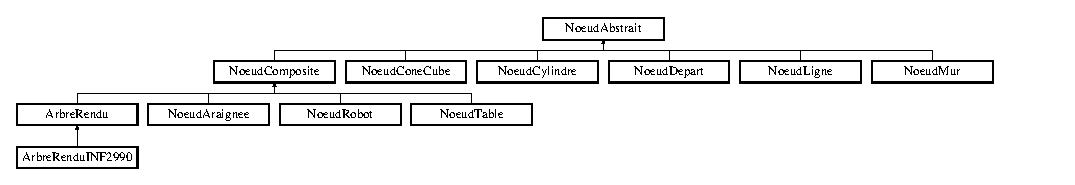
\includegraphics[height=1.866667cm]{class_noeud_abstrait}
\end{center}
\end{figure}
\subsection*{Public Member Functions}
\begin{DoxyCompactItemize}
\item 
\hyperlink{group__inf2990_gad1eae42fe2bccef56f55b8a52726657f}{Noeud\+Abstrait} (const std\+::string \&type=\{\})
\begin{DoxyCompactList}\small\item\em Constructeur. \end{DoxyCompactList}\item 
\hyperlink{group__inf2990_gae7bea8d23c4dad60c334fc6806d08d01}{Noeud\+Abstrait} (const \hyperlink{class_noeud_abstrait}{Noeud\+Abstrait} \&n0)
\begin{DoxyCompactList}\small\item\em Constructeur par copie. \end{DoxyCompactList}\item 
virtual \hyperlink{group__inf2990_ga0ab3f7ab838e8349113da5074abcdc3a}{$\sim$\+Noeud\+Abstrait} ()
\begin{DoxyCompactList}\small\item\em Destructeur. \end{DoxyCompactList}\item 
\hyperlink{class_noeud_abstrait}{Noeud\+Abstrait} $\ast$ \hyperlink{group__inf2990_gaa2ac8c4cd02d88c312b92c65e07ed6d9}{obtenir\+Parent} ()
\begin{DoxyCompactList}\small\item\em Obtient le parent de ce noeud. \end{DoxyCompactList}\item 
const \hyperlink{class_noeud_abstrait}{Noeud\+Abstrait} $\ast$ \hyperlink{group__inf2990_gaf063d208bc4764b1fd2c4e76ec0469b9}{obtenir\+Parent} () const 
\begin{DoxyCompactList}\small\item\em Obtient le parent de ce noeud (version constante). \end{DoxyCompactList}\item 
void \hyperlink{group__inf2990_ga7787ab59ecc1e6119287459a7154f307}{assigner\+Parent} (\hyperlink{class_noeud_abstrait}{Noeud\+Abstrait} $\ast$parent)
\begin{DoxyCompactList}\small\item\em Assigne le parent de ce noeud. \end{DoxyCompactList}\item 
const glm\+::dvec3 \& \hyperlink{group__inf2990_ga62d73f67c3b33e2cb106630bd1736a58}{obtenir\+Position\+Relative} () const 
\begin{DoxyCompactList}\small\item\em Obtient la position relative du noeud. \end{DoxyCompactList}\item 
void \hyperlink{group__inf2990_ga11e12e42b05a5327c92cd7fd1b7e5a24}{assigner\+Position\+Relative} (const glm\+::dvec3 \&position\+Relative)
\begin{DoxyCompactList}\small\item\em Assigne la position relative du noeud. \end{DoxyCompactList}\item 
const glm\+::dvec3 \& \hyperlink{group__inf2990_ga5e57e4e6ac1df01d25098fbeb7fcc56d}{obtenir\+Position\+Initiale} () const 
\begin{DoxyCompactList}\small\item\em Obtient la position initiale du noeud. \end{DoxyCompactList}\item 
void \hyperlink{group__inf2990_ga18ba04a32eaa8942418950a647e5e717}{assigner\+Position\+Initiale} (const glm\+::dvec3 \&position\+Initiale)
\begin{DoxyCompactList}\small\item\em Assigne la position initiale du noeud. \end{DoxyCompactList}\item 
const float \hyperlink{group__inf2990_ga9f5f0864e56b552efe95e693c198a3b4}{obtenir\+Angle} () const 
\begin{DoxyCompactList}\small\item\em Obtient l\textquotesingle{}angle du noeud. \end{DoxyCompactList}\item 
void \hyperlink{group__inf2990_ga7977957d758ca590a057aa33d76e5e75}{assigner\+Angle} (const float angle)
\begin{DoxyCompactList}\small\item\em Assigne l\textquotesingle{}angle du noeud. \end{DoxyCompactList}\item 
const float \hyperlink{group__inf2990_ga61797fb6a426150891203ea91e3f2cb8}{obtenir\+Angle\+Initial} () const 
\begin{DoxyCompactList}\small\item\em Obtient l\textquotesingle{}angle initial du noeud. \end{DoxyCompactList}\item 
void \hyperlink{group__inf2990_gaf0e7fd3676087b70949012a945000509}{assigner\+Angle\+Initial} (const float angle\+Initial)
\begin{DoxyCompactList}\small\item\em Assigne l\textquotesingle{}angle initial du noeud. \end{DoxyCompactList}\item 
glm\+::fvec3 \hyperlink{group__inf2990_ga153a0490acbbaeda4647496e51d37894}{get\+Scale} () const 
\begin{DoxyCompactList}\small\item\em Obtient l\textquotesingle{}échelle du noeud. \end{DoxyCompactList}\item 
virtual void \hyperlink{group__inf2990_gaef8fd99796f85418adac496160a3350b}{set\+Scale} (const glm\+::fvec3 scale)
\begin{DoxyCompactList}\small\item\em Assigne l\textquotesingle{}échelle du noeud. \end{DoxyCompactList}\item 
glm\+::fvec3 \hyperlink{group__inf2990_gab229ec2d195c9e9bfa1a4c0f80b582ca}{get\+Scale\+Initial} () const 
\begin{DoxyCompactList}\small\item\em Obtient l\textquotesingle{}échelle initiale du noeud. \end{DoxyCompactList}\item 
virtual void \hyperlink{group__inf2990_gae51f2e4da1ff9308a55324d4aafd72db}{set\+Scale\+Initial} (const glm\+::fvec3 scale)
\begin{DoxyCompactList}\small\item\em Assigne l\textquotesingle{}échelle initiale du noeud. \end{DoxyCompactList}\item 
const std\+::string \& \hyperlink{group__inf2990_ga2df7c53ab456cc88bce73f7eb913e3e6}{obtenir\+Type} () const 
\begin{DoxyCompactList}\small\item\em Obtient le type du noeud. \end{DoxyCompactList}\item 
void \hyperlink{group__inf2990_gad5205d1e1b63fb66175a8580261d5eea}{assigner\+Affiche} (bool affiche)
\begin{DoxyCompactList}\small\item\em Écrit l\textquotesingle{}état de l\textquotesingle{}affichage du du noeud. \end{DoxyCompactList}\item 
bool \hyperlink{group__inf2990_ga07fc02e86d59ccd2680f9e5f5b8e373d}{est\+Affiche} () const 
\begin{DoxyCompactList}\small\item\em Vérifie si le noeud se fait afficher. \end{DoxyCompactList}\item 
void \hyperlink{group__inf2990_ga0f39647390d357d8662a870f0c76242c}{assigner\+Selection} (bool selectionne)
\begin{DoxyCompactList}\small\item\em Écrit l\textquotesingle{}état de la sélection du noeud. \end{DoxyCompactList}\item 
bool \hyperlink{group__inf2990_ga8fb7a3313ce4d361ef7ec8e45ba8add5}{est\+Selectionne} () const 
\begin{DoxyCompactList}\small\item\em Vérifie si le noeud est sélectionné. \end{DoxyCompactList}\item 
void \hyperlink{group__inf2990_ga397add0bac7ec3b842598a2085990b7d}{assigner\+Est\+Selectionnable} (bool selectionnable)
\begin{DoxyCompactList}\small\item\em Écrit si le noeud peut être sélectionné ou non. \end{DoxyCompactList}\item 
bool \hyperlink{group__inf2990_gaa3f3a34571af62de0da5db2d8f54f690}{est\+Selectionnable} () const 
\begin{DoxyCompactList}\small\item\em Vérifie si le noeud est sélectionnable. \end{DoxyCompactList}\item 
void \hyperlink{group__inf2990_gabb7f3756a4094dc588690126ec0703d3}{assigner\+Est\+Enregistrable} (bool enregistrable)
\begin{DoxyCompactList}\small\item\em Écrit si le noeud peut être enregistré ou non. \end{DoxyCompactList}\item 
bool \hyperlink{group__inf2990_ga6a6af3639f1b4e3e33a126703376dcec}{est\+Enregistrable} () const 
\begin{DoxyCompactList}\small\item\em Vérifie si le noeud est enregistrable. \end{DoxyCompactList}\item 
void \hyperlink{group__inf2990_ga1f533acce98fbad7fa82758ccaea55ff}{assigner\+Objet\+Rendu} (\hyperlink{classmodele_1_1_modele3_d}{modele\+::\+Modele3\+D} const $\ast$modele, \hyperlink{classopengl_1_1_v_b_o}{opengl\+::\+V\+B\+O} const $\ast$liste)
\begin{DoxyCompactList}\small\item\em Assigne le modèle3\+D et la liste d\textquotesingle{}affichage du noeud courant. \end{DoxyCompactList}\item 
\hypertarget{group__inf2990_gacf20d310cd93a8ba2c3e4bc182398853}{}const \hyperlink{classmodele_1_1_modele3_d}{modele\+::\+Modele3\+D} $\ast$ \hyperlink{group__inf2990_gacf20d310cd93a8ba2c3e4bc182398853}{get\+Modele} ()\label{group__inf2990_gacf20d310cd93a8ba2c3e4bc182398853}

\begin{DoxyCompactList}\small\item\em Retourne le modèle 3\+D du coeud. \end{DoxyCompactList}\item 
virtual unsigned int \hyperlink{group__inf2990_gad854800087fd6c13f1a63589caefb41d}{calculer\+Profondeur} () const 
\begin{DoxyCompactList}\small\item\em Calcule la profondeur de l\textquotesingle{}arbre sous le noeud courant. \end{DoxyCompactList}\item 
virtual void \hyperlink{group__inf2990_ga55435ee83860c6a2101334ba67bbd9b6}{vider} ()
\begin{DoxyCompactList}\small\item\em Vide le noeud de ses enfants. \end{DoxyCompactList}\item 
virtual void \hyperlink{group__inf2990_ga2ab3dc520026d1ad77aa848981688bfd}{effacer} (const \hyperlink{class_noeud_abstrait}{Noeud\+Abstrait} $\ast$noeud)
\begin{DoxyCompactList}\small\item\em Efface le noeud passé en paramètre. \end{DoxyCompactList}\item 
virtual const \hyperlink{class_noeud_abstrait}{Noeud\+Abstrait} $\ast$ \hyperlink{group__inf2990_gaeda0df98faf404765d985fcde60fb924}{chercher} (const std\+::string \&type\+Noeud) const 
\begin{DoxyCompactList}\small\item\em Cherche un noeud par le type (sur un noeud constant). \end{DoxyCompactList}\item 
virtual \hyperlink{class_noeud_abstrait}{Noeud\+Abstrait} $\ast$ \hyperlink{group__inf2990_ga0868ae108165b071f6c8a68a7265c770}{chercher} (const std\+::string \&type\+Noeud)
\begin{DoxyCompactList}\small\item\em Cherche un noeud par le type. \end{DoxyCompactList}\item 
virtual const \hyperlink{class_noeud_abstrait}{Noeud\+Abstrait} $\ast$ \hyperlink{group__inf2990_gac334b078c318e39a065b85572778bf13}{chercher} (unsigned int indice) const 
\begin{DoxyCompactList}\small\item\em Cherche un noeud enfant selon l\textquotesingle{}indice (sur un noeud constant). \end{DoxyCompactList}\item 
virtual \hyperlink{class_noeud_abstrait}{Noeud\+Abstrait} $\ast$ \hyperlink{group__inf2990_ga13f7e9a637f7439b1a0cec0c49f6fa88}{chercher} (unsigned int indice)
\begin{DoxyCompactList}\small\item\em Cherche un noeud enfant selon l\textquotesingle{}indice. \end{DoxyCompactList}\item 
virtual bool \hyperlink{group__inf2990_ga7051399643afa57468ef07444a085a85}{ajouter} (std\+::unique\+\_\+ptr$<$ \hyperlink{class_noeud_abstrait}{Noeud\+Abstrait} $>$ enfant)
\begin{DoxyCompactList}\small\item\em Ajoute un noeud enfant. \end{DoxyCompactList}\item 
virtual unsigned int \hyperlink{group__inf2990_gad5a99959e905fc2d9f0fef16a02546a2}{obtenir\+Nombre\+Enfants} () const 
\begin{DoxyCompactList}\small\item\em Obtient le nombre d\textquotesingle{}enfants du noeud. \end{DoxyCompactList}\item 
virtual void \hyperlink{group__inf2990_ga2516eef94f98d4951baff6fd45020725}{inverser\+Selection} ()
\begin{DoxyCompactList}\small\item\em Changer la sélection du noeud. \end{DoxyCompactList}\item 
virtual void \hyperlink{group__inf2990_gaf6440c1b4ab6861f0ace6ba410c1fc84}{effacer\+Selection} ()
\begin{DoxyCompactList}\small\item\em Efface les enfants sélectionnés. \end{DoxyCompactList}\item 
virtual void \hyperlink{group__inf2990_gaa9b1fa06dad2695ea6870411c62652b3}{selectionner\+Tout} ()
\begin{DoxyCompactList}\small\item\em Sélectionne tous les enfants de même que le noeud. \end{DoxyCompactList}\item 
virtual void \hyperlink{group__inf2990_ga4f942bd122fc3402537ecac737c5248a}{deselectionner\+Tout} ()
\begin{DoxyCompactList}\small\item\em Désélectionne tous les enfants de même que le noeud. \end{DoxyCompactList}\item 
virtual bool \hyperlink{group__inf2990_gae7c702b865babd20ddd30dd776adc82b}{selection\+Existe} () const 
\begin{DoxyCompactList}\small\item\em Vérifier si le noeud ou un de ses enfants est sélectionné. \end{DoxyCompactList}\item 
virtual void \hyperlink{group__inf2990_ga13a97383c2081b405fc2e0d97cff80df}{changer\+Mode\+Polygones} (bool est\+Force)
\begin{DoxyCompactList}\small\item\em Change le mode d\textquotesingle{}affichage des polygones. \end{DoxyCompactList}\item 
virtual void \hyperlink{group__inf2990_ga726d9d0a524939f405aeeac3fbd06666}{assigner\+Mode\+Polygones} (G\+Lenum mode\+Polygones)
\begin{DoxyCompactList}\small\item\em Assigne le mode d\textquotesingle{}affichage des polygones. \end{DoxyCompactList}\item 
virtual void \hyperlink{group__inf2990_gae789271ea41032d717b8e4300be05de0}{afficher} () const 
\begin{DoxyCompactList}\small\item\em Affiche le noeud. \end{DoxyCompactList}\item 
virtual void \hyperlink{group__inf2990_ga330df455c8b08440d3c8e64d0a480391}{afficher\+Concret} () const 
\begin{DoxyCompactList}\small\item\em Affiche le noeud de manière concrète. \end{DoxyCompactList}\item 
virtual void \hyperlink{group__inf2990_gadc6ebe69894dbb682fdd0ecb1b6c11e9}{animer} (float dt)
\begin{DoxyCompactList}\small\item\em Anime le noeud. \end{DoxyCompactList}\item 
\hypertarget{class_noeud_abstrait_ac166d3266931e3bb81d4df1617108340}{}virtual void {\bfseries accept} (\hyperlink{class_tool}{Tool} \&visitor)=0\label{class_noeud_abstrait_ac166d3266931e3bb81d4df1617108340}

\item 
virtual \hyperlink{class_savable}{Savable} \hyperlink{group__inf2990_ga1729231ec41b3ba4d6668eba101ead44}{get\+Savable\+Data} ()
\item 
\hypertarget{group__inf2990_ga78bba41d63a1a2a621e82c8247180b42}{}virtual void {\bfseries assigner\+Selection\+Enfants} (G\+Ldouble x, G\+Ldouble y, G\+Ldouble z, bool keep\+Others)\label{group__inf2990_ga78bba41d63a1a2a621e82c8247180b42}

\item 
virtual void \hyperlink{group__inf2990_ga7304995555625461f49b1e75dd81e888}{assigner\+Selection\+Enfants} (glm\+::ivec2 debut, glm\+::ivec2 fin, bool keep\+Others)
\item 
virtual void \hyperlink{group__inf2990_gabd4eaa5eef18dc3a12fa140086238b5f}{afficher\+Selections\+Console} ()
\item 
virtual void \hyperlink{group__inf2990_ga233fd4600812176c557bb94ea04da5c9}{update\+Creation} (glm\+::dvec3 cursor)
\end{DoxyCompactItemize}
{\bf }\par
\begin{DoxyCompactItemize}
\item 
virtual bool \hyperlink{group__inf2990_ga2e40156a7ff6dd734c61de990db1bfe0}{click\+Hit} (G\+Ldouble x, G\+Ldouble y, G\+Ldouble z)
\item 
virtual bool \hyperlink{group__inf2990_gad1d1a9c6adcedfcd5eda6c6d4e67a50f}{click\+Hit} (glm\+::ivec2 debut, glm\+::ivec2 fin)
\end{DoxyCompactItemize}

\subsection*{Protected Attributes}
\begin{DoxyCompactItemize}
\item 
\hypertarget{class_noeud_abstrait_ad53da47a60f4b4fbbd400234cbdcb06b}{}std\+::string \hyperlink{class_noeud_abstrait_ad53da47a60f4b4fbbd400234cbdcb06b}{type\+\_\+}\label{class_noeud_abstrait_ad53da47a60f4b4fbbd400234cbdcb06b}

\begin{DoxyCompactList}\small\item\em Type du noeud. \end{DoxyCompactList}\item 
\hypertarget{class_noeud_abstrait_aa2b57eeb848bc8cb48562788daf81d3e}{}G\+Lenum \hyperlink{class_noeud_abstrait_aa2b57eeb848bc8cb48562788daf81d3e}{mode\+Polygones\+\_\+} \{ G\+L\+\_\+\+F\+I\+L\+L \}\label{class_noeud_abstrait_aa2b57eeb848bc8cb48562788daf81d3e}

\begin{DoxyCompactList}\small\item\em Mode d\textquotesingle{}affichage des polygones. \end{DoxyCompactList}\item 
\hypertarget{class_noeud_abstrait_ae8a50095413ac131cd6d07a384a9ff5d}{}glm\+::dvec3 \hyperlink{class_noeud_abstrait_ae8a50095413ac131cd6d07a384a9ff5d}{position\+Relative\+\_\+}\label{class_noeud_abstrait_ae8a50095413ac131cd6d07a384a9ff5d}

\begin{DoxyCompactList}\small\item\em Position relative du noeud. \end{DoxyCompactList}\item 
\hypertarget{class_noeud_abstrait_a9ac4861933dc8eedb4f5abe6cdc934b8}{}glm\+::dvec3 \hyperlink{class_noeud_abstrait_a9ac4861933dc8eedb4f5abe6cdc934b8}{position\+Initiale\+\_\+}\label{class_noeud_abstrait_a9ac4861933dc8eedb4f5abe6cdc934b8}

\begin{DoxyCompactList}\small\item\em Position initiale du noeud. \end{DoxyCompactList}\item 
\hypertarget{class_noeud_abstrait_a69f867797b7cdc93fbcb5b4d9ae3deee}{}float \hyperlink{class_noeud_abstrait_a69f867797b7cdc93fbcb5b4d9ae3deee}{angle\+Rotation\+\_\+} \{ 0.f \}\label{class_noeud_abstrait_a69f867797b7cdc93fbcb5b4d9ae3deee}

\begin{DoxyCompactList}\small\item\em Angle de rotation. \end{DoxyCompactList}\item 
\hypertarget{class_noeud_abstrait_a690912f58567f89c7add07a684578be3}{}float \hyperlink{class_noeud_abstrait_a690912f58567f89c7add07a684578be3}{angle\+Rotation\+Initial\+\_\+} \{ 0.f \}\label{class_noeud_abstrait_a690912f58567f89c7add07a684578be3}

\begin{DoxyCompactList}\small\item\em Angle de rotation initial. \end{DoxyCompactList}\item 
\hypertarget{class_noeud_abstrait_af35c9a382963f536980e17427cffb846}{}glm\+::fvec3 \hyperlink{class_noeud_abstrait_af35c9a382963f536980e17427cffb846}{scale\+\_\+}\label{class_noeud_abstrait_af35c9a382963f536980e17427cffb846}

\begin{DoxyCompactList}\small\item\em Échelle (scale) \end{DoxyCompactList}\item 
\hypertarget{class_noeud_abstrait_af2cfa59c032dbbe59123edbc76ab861c}{}glm\+::fvec3 {\bfseries scale\+Initial\+\_\+}\label{class_noeud_abstrait_af2cfa59c032dbbe59123edbc76ab861c}

\item 
\hypertarget{class_noeud_abstrait_a20af11e8041b0af8a34b6f041bb24c7f}{}bool \hyperlink{class_noeud_abstrait_a20af11e8041b0af8a34b6f041bb24c7f}{affiche\+\_\+} \{ true \}\label{class_noeud_abstrait_a20af11e8041b0af8a34b6f041bb24c7f}

\begin{DoxyCompactList}\small\item\em Vrai si on doit afficher le noeud. \end{DoxyCompactList}\item 
\hypertarget{class_noeud_abstrait_a7b2d2410f947987765a9ef41fedcc703}{}bool \hyperlink{class_noeud_abstrait_a7b2d2410f947987765a9ef41fedcc703}{selectionne\+\_\+} \{ false \}\label{class_noeud_abstrait_a7b2d2410f947987765a9ef41fedcc703}

\begin{DoxyCompactList}\small\item\em Sélection du noeud. \end{DoxyCompactList}\item 
\hypertarget{class_noeud_abstrait_a2e5d12f2a106f410e149263fa72a530f}{}bool \hyperlink{class_noeud_abstrait_a2e5d12f2a106f410e149263fa72a530f}{selectionnable\+\_\+} \{ true \}\label{class_noeud_abstrait_a2e5d12f2a106f410e149263fa72a530f}

\begin{DoxyCompactList}\small\item\em Vrai si le noeud est sélectionnable. \end{DoxyCompactList}\item 
\hypertarget{class_noeud_abstrait_aa4b43e83161e8650b8810c8e29f0c985}{}bool \hyperlink{class_noeud_abstrait_aa4b43e83161e8650b8810c8e29f0c985}{enregistrable\+\_\+} \{ true \}\label{class_noeud_abstrait_aa4b43e83161e8650b8810c8e29f0c985}

\begin{DoxyCompactList}\small\item\em Détermine si l\textquotesingle{}objet peut être sauvegardé en X\+M\+L. \end{DoxyCompactList}\item 
\hypertarget{class_noeud_abstrait_a002558def0146fea8c413c7928b962a1}{}\hyperlink{class_noeud_abstrait}{Noeud\+Abstrait} $\ast$ \hyperlink{class_noeud_abstrait_a002558def0146fea8c413c7928b962a1}{parent\+\_\+} \{ nullptr \}\label{class_noeud_abstrait_a002558def0146fea8c413c7928b962a1}

\begin{DoxyCompactList}\small\item\em Pointeur vers le parent. \end{DoxyCompactList}\item 
\hypertarget{class_noeud_abstrait_abc3dc8e24578214b7c6081be3246645e}{}\hyperlink{classmodele_1_1_modele3_d}{modele\+::\+Modele3\+D} const $\ast$ \hyperlink{class_noeud_abstrait_abc3dc8e24578214b7c6081be3246645e}{modele\+\_\+}\label{class_noeud_abstrait_abc3dc8e24578214b7c6081be3246645e}

\begin{DoxyCompactList}\small\item\em Modèle 3\+D correspondant à ce noeud. \end{DoxyCompactList}\item 
\hypertarget{class_noeud_abstrait_ae53668f6c4df669a0923a16b3cb84f83}{}\hyperlink{classopengl_1_1_v_b_o}{opengl\+::\+V\+B\+O} const $\ast$ \hyperlink{class_noeud_abstrait_ae53668f6c4df669a0923a16b3cb84f83}{vbo\+\_\+}\label{class_noeud_abstrait_ae53668f6c4df669a0923a16b3cb84f83}

\begin{DoxyCompactList}\small\item\em Storage pour le dessin du modèle. \end{DoxyCompactList}\end{DoxyCompactItemize}


\subsection{Detailed Description}
Classe de base du patron composite utilisée pour créer l\textquotesingle{}arbre de rendu. 

Cette classe abstraite comprend l\textquotesingle{}interface de base que doivent implanter tous les noeuds pouvant être présent dans l\textquotesingle{}arbre de rendu.

\begin{DoxyAuthor}{Author}
D\+G\+I-\/2990 
\end{DoxyAuthor}
\begin{DoxyDate}{Date}
2007-\/01-\/24 
\end{DoxyDate}


The documentation for this class was generated from the following files\+:\begin{DoxyCompactItemize}
\item 
Sources/\+D\+L\+L/\+Arbre/\+Noeuds/\hyperlink{_noeud_abstrait_8h}{Noeud\+Abstrait.\+h}\item 
Sources/\+D\+L\+L/\+Arbre/\+Noeuds/\hyperlink{_noeud_abstrait_8cpp}{Noeud\+Abstrait.\+cpp}\item 
Sources/\+D\+L\+L/\+Arbre/\+Noeuds/\hyperlink{_noeud_depart_8cpp}{Noeud\+Depart.\+cpp}\item 
Sources/\+D\+L\+L/\+Arbre/\+Noeuds/\hyperlink{_noeud_table_8cpp}{Noeud\+Table.\+cpp}\end{DoxyCompactItemize}

\hypertarget{class_noeud_abstrait_test}{\section{Référence de la classe Noeud\-Abstrait\-Test}
\label{class_noeud_abstrait_test}\index{Noeud\-Abstrait\-Test@{Noeud\-Abstrait\-Test}}
}


Classe de test cppunit pour tester le bon fonctionnement des méthodes de la classe \hyperlink{class_noeud_abstrait}{Noeud\-Abstrait}.  




{\ttfamily \#include $<$Noeud\-Abstrait\-Test.\-h$>$}

Graphe d'héritage de Noeud\-Abstrait\-Test\-:\begin{figure}[H]
\begin{center}
\leavevmode
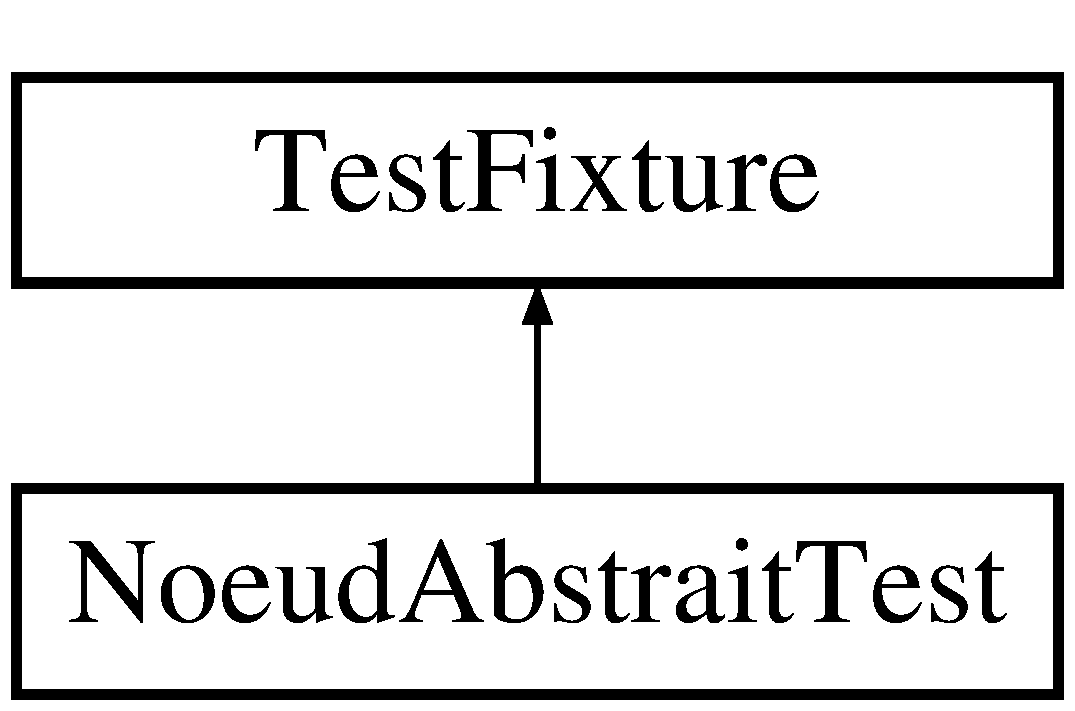
\includegraphics[height=2.000000cm]{class_noeud_abstrait_test}
\end{center}
\end{figure}
\subsection*{Fonctions membres publiques}
\begin{DoxyCompactItemize}
\item 
void \hyperlink{group__inf2990_ga4d2fe388f550ba374823d09b5c8ebe77}{set\-Up} ()
\begin{DoxyCompactList}\small\item\em Traitement à effectuer pour initialiser cette suite de tests. \end{DoxyCompactList}\item 
void \hyperlink{group__inf2990_ga2c5c558ff7e40386c724a55b670af417}{tear\-Down} ()
\begin{DoxyCompactList}\small\item\em Traitement à effectuer pour 'finaliser' cette suite de tests. \end{DoxyCompactList}\item 
void \hyperlink{group__inf2990_gaed7a5423d2a3a7518aef743f17d32ccd}{test\-Position\-Relative} ()
\begin{DoxyCompactList}\small\item\em Cas de test\-: écriture/lecture de la position relative. \end{DoxyCompactList}\item 
void \hyperlink{group__inf2990_gadf554a62266cc21c7c48f6a27ad7c752}{test\-Type} ()
\begin{DoxyCompactList}\small\item\em Cas de test\-: type de noeud. \end{DoxyCompactList}\item 
void \hyperlink{group__inf2990_gac044744b04574c86418a57b39e3238ff}{test\-Selection} ()
\begin{DoxyCompactList}\small\item\em Cas de test\-: définition/obtention des états de sélection du noeud. \end{DoxyCompactList}\item 
void \hyperlink{group__inf2990_ga0e65b00620e79646a9efd8a93c4fc650}{test\-Enfants} ()
\begin{DoxyCompactList}\small\item\em Cas de test\-: s'assurer que le noeud abstrait n'a pas d'enfant. \end{DoxyCompactList}\item 
void \hyperlink{group__inf2990_gab9182c635c672eb2ade3f2b2b5043244}{test\-Scale} ()
\begin{DoxyCompactList}\small\item\em Cas de test\-: s'assurer que les restrictions sur l'échelle sont respectées. \end{DoxyCompactList}\end{DoxyCompactItemize}


\subsection{Description détaillée}
Classe de test cppunit pour tester le bon fonctionnement des méthodes de la classe \hyperlink{class_noeud_abstrait}{Noeud\-Abstrait}. 

\begin{DoxyAuthor}{Auteur}
Julien Gascon-\/\-Samson 
\end{DoxyAuthor}
\begin{DoxyDate}{Date}
2011-\/07-\/16 
\end{DoxyDate}


La documentation de cette classe a été générée à partir des fichiers suivants \-:\begin{DoxyCompactItemize}
\item 
C\-:/\-Users/saron/\-Documents/inf2990-\/01/\-Sources/\-D\-L\-L/\-Tests/\hyperlink{_noeud_abstrait_test_8h}{Noeud\-Abstrait\-Test.\-h}\item 
C\-:/\-Users/saron/\-Documents/inf2990-\/01/\-Sources/\-D\-L\-L/\-Tests/\hyperlink{_noeud_abstrait_test_8cpp}{Noeud\-Abstrait\-Test.\-cpp}\end{DoxyCompactItemize}

\hypertarget{class_noeud_araignee}{}\section{Noeud\+Araignee Class Reference}
\label{class_noeud_araignee}\index{Noeud\+Araignee@{Noeud\+Araignee}}


Classe qui représente un exemple de noeud de l\textquotesingle{}arbre de rendu.  




{\ttfamily \#include $<$Noeud\+Araignee.\+h$>$}

Inheritance diagram for Noeud\+Araignee\+:\begin{figure}[H]
\begin{center}
\leavevmode
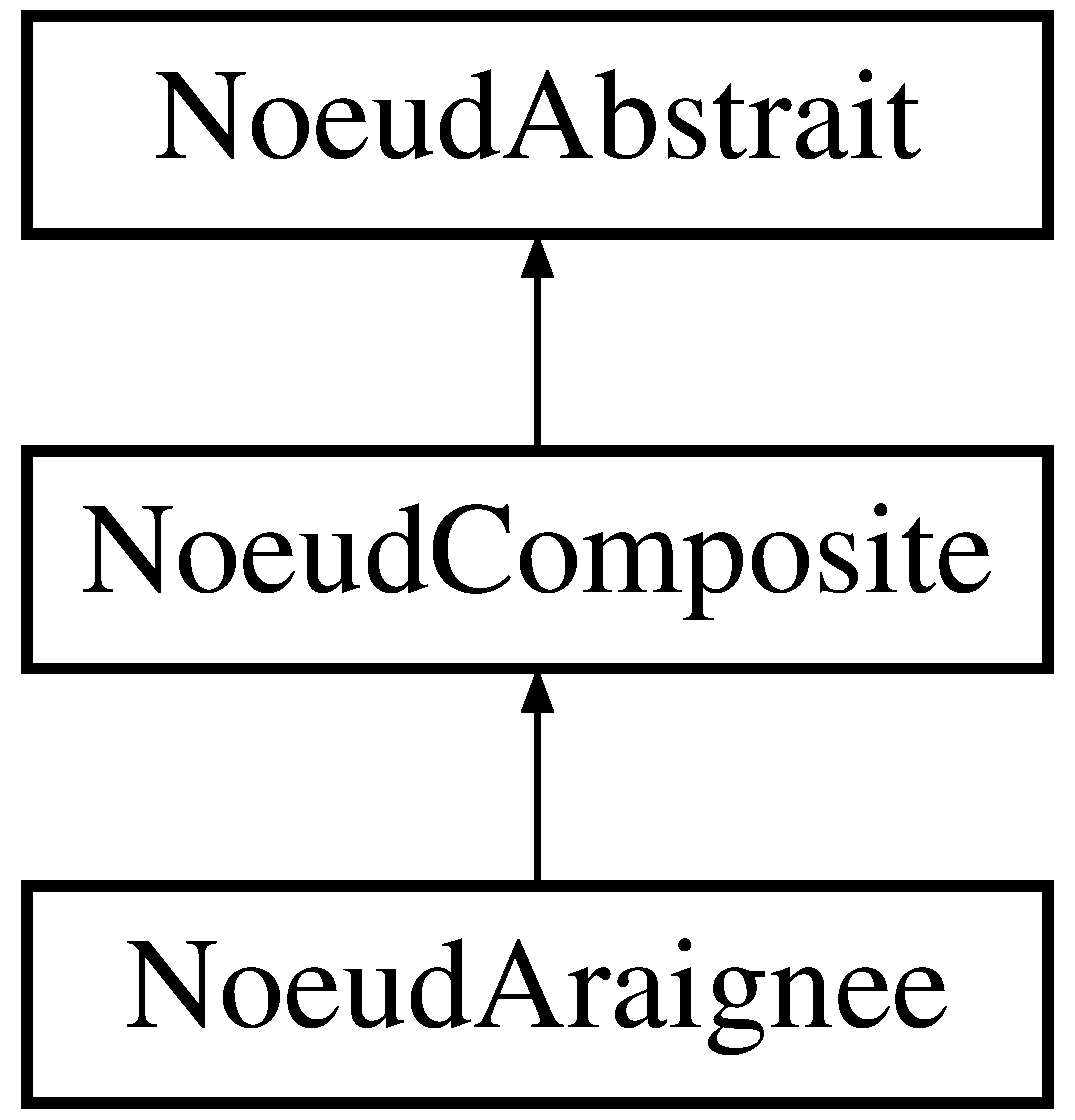
\includegraphics[height=3.000000cm]{class_noeud_araignee}
\end{center}
\end{figure}
\subsection*{Public Member Functions}
\begin{DoxyCompactItemize}
\item 
\hyperlink{group__inf2990_ga0ca3d14d5baf9c6879ac53918cc54ba5}{Noeud\+Araignee} (const std\+::string \&type\+Noeud)
\begin{DoxyCompactList}\small\item\em Constructeur à partir du type du noeud. \end{DoxyCompactList}\item 
\hyperlink{group__inf2990_ga78bf0250c601da26edb8cd8f2cddec10}{$\sim$\+Noeud\+Araignee} ()
\begin{DoxyCompactList}\small\item\em Destructeur. \end{DoxyCompactList}\item 
virtual void \hyperlink{group__inf2990_ga4f9e7fbb424a0cb18e01ab12a092fc02}{afficher\+Concret} () const 
\begin{DoxyCompactList}\small\item\em Affiche le cube. \end{DoxyCompactList}\item 
\hypertarget{group__inf2990_gae3f4c490330d597a18975014c06a05ca}{}virtual void \hyperlink{group__inf2990_gae3f4c490330d597a18975014c06a05ca}{animer} (float temps)\label{group__inf2990_gae3f4c490330d597a18975014c06a05ca}

\begin{DoxyCompactList}\small\item\em Effectue l\textquotesingle{}animation du cube. \end{DoxyCompactList}\end{DoxyCompactItemize}
\subsection*{Additional Inherited Members}


\subsection{Detailed Description}
Classe qui représente un exemple de noeud de l\textquotesingle{}arbre de rendu. 

\begin{DoxyAuthor}{Author}
Julien Gascon-\/\+Samson 
\end{DoxyAuthor}
\begin{DoxyDate}{Date}
2011-\/05-\/19 
\end{DoxyDate}


The documentation for this class was generated from the following files\+:\begin{DoxyCompactItemize}
\item 
C\+:/\+Users/\+Louis/workspace/inf2990-\/01/\+Sources/\+D\+L\+L/\+Arbre/\+Noeuds/\hyperlink{_noeud_araignee_8h}{Noeud\+Araignee.\+h}\item 
C\+:/\+Users/\+Louis/workspace/inf2990-\/01/\+Sources/\+D\+L\+L/\+Arbre/\+Noeuds/\hyperlink{_noeud_araignee_8cpp}{Noeud\+Araignee.\+cpp}\end{DoxyCompactItemize}

\hypertarget{class_noeud_composite}{}\section{Noeud\+Composite Class Reference}
\label{class_noeud_composite}\index{Noeud\+Composite@{Noeud\+Composite}}


Implantation d\textquotesingle{}un noeud du patron composite qui peut posséder des enfants.  




{\ttfamily \#include $<$Noeud\+Composite.\+h$>$}

Inheritance diagram for Noeud\+Composite\+:\begin{figure}[H]
\begin{center}
\leavevmode
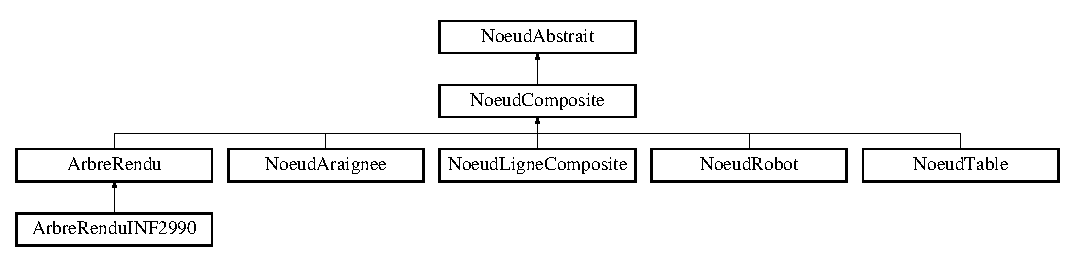
\includegraphics[height=4.000000cm]{class_noeud_composite}
\end{center}
\end{figure}
\subsection*{Public Member Functions}
\begin{DoxyCompactItemize}
\item 
\hypertarget{group__inf2990_ga9493824e1865121cb75097a28132573b}{}\hyperlink{group__inf2990_ga9493824e1865121cb75097a28132573b}{Noeud\+Composite} (std\+::string type=\{\})\label{group__inf2990_ga9493824e1865121cb75097a28132573b}

\begin{DoxyCompactList}\small\item\em Constructeur. \end{DoxyCompactList}\item 
\hypertarget{class_noeud_composite_af221c032fbc9d58e3344ee1b122095cd}{}virtual \hyperlink{class_noeud_composite_af221c032fbc9d58e3344ee1b122095cd}{$\sim$\+Noeud\+Composite} ()=default\label{class_noeud_composite_af221c032fbc9d58e3344ee1b122095cd}

\begin{DoxyCompactList}\small\item\em Destructeur. \end{DoxyCompactList}\item 
unsigned int \hyperlink{group__inf2990_gaf9a41e3632a6a321388c7705cfbece21}{calculer\+Profondeur} () const  override
\begin{DoxyCompactList}\small\item\em Calcule la profondeur de l\textquotesingle{}arbre sous le noeud courant. \end{DoxyCompactList}\item 
void \hyperlink{group__inf2990_gaede690fd0ecafe4244479ca4f054a65f}{vider} () override
\begin{DoxyCompactList}\small\item\em Vide le noeud de ses enfants. \end{DoxyCompactList}\item 
void \hyperlink{group__inf2990_gad6e967709392313acafee99a9a05a5a5}{effacer} (const \hyperlink{class_noeud_abstrait}{Noeud\+Abstrait} $\ast$noeud) override
\begin{DoxyCompactList}\small\item\em Efface le noeud passé en paramètre. \end{DoxyCompactList}\item 
const \hyperlink{class_noeud_abstrait}{Noeud\+Abstrait} $\ast$ \hyperlink{group__inf2990_ga10f285f39739539bbf9f8cb4b6383414}{chercher} (const std\+::string \&type\+Noeud) const  override
\begin{DoxyCompactList}\small\item\em Cherche un noeud par le type (sur un noeud constant). \end{DoxyCompactList}\item 
\hyperlink{class_noeud_abstrait}{Noeud\+Abstrait} $\ast$ \hyperlink{group__inf2990_gad7f54e2eb26b9ce59fbaedb2d0090f0e}{chercher} (const std\+::string \&type\+Noeud) override
\begin{DoxyCompactList}\small\item\em Cherche un noeud par le type. \end{DoxyCompactList}\item 
const \hyperlink{class_noeud_abstrait}{Noeud\+Abstrait} $\ast$ \hyperlink{group__inf2990_gaa522a1f30c1d045745ed04b680e2649b}{chercher} (unsigned int indice) const  override
\begin{DoxyCompactList}\small\item\em Cherche un noeud enfant selon l\textquotesingle{}indice (sur un noeud constant). \end{DoxyCompactList}\item 
\hyperlink{class_noeud_abstrait}{Noeud\+Abstrait} $\ast$ \hyperlink{group__inf2990_ga9f6cf297ac93d75711e1ae85cb0a69ed}{chercher} (unsigned int indice) override
\begin{DoxyCompactList}\small\item\em Cherche un noeud enfant selon l\textquotesingle{}indice. \end{DoxyCompactList}\item 
bool \hyperlink{group__inf2990_ga5651862ed875690375d9a82a06ecdcb2}{ajouter} (std\+::unique\+\_\+ptr$<$ \hyperlink{class_noeud_abstrait}{Noeud\+Abstrait} $>$ enfant) override
\begin{DoxyCompactList}\small\item\em Ajoute un noeud enfant. \end{DoxyCompactList}\item 
unsigned int \hyperlink{group__inf2990_ga4cb7898e88b8726f93dfe588105472d4}{obtenir\+Nombre\+Enfants} () const  override
\begin{DoxyCompactList}\small\item\em Obtient le nombre d\textquotesingle{}enfants du noeud. \end{DoxyCompactList}\item 
void \hyperlink{group__inf2990_ga7e3aa1018378eb5e0342b2fe530783cc}{effacer\+Selection} () override
\begin{DoxyCompactList}\small\item\em Efface les enfants sélectionnés. \end{DoxyCompactList}\item 
void \hyperlink{group__inf2990_ga1fb05aa01553f1fa6738711ab172efb6}{selectionner\+Tout} () override
\begin{DoxyCompactList}\small\item\em Sélectionne tous les enfants de même que le noeud. \end{DoxyCompactList}\item 
void \hyperlink{group__inf2990_ga98d6f93f7dc06301f8909e8cf31e3e9e}{deselectionner\+Tout} () override
\begin{DoxyCompactList}\small\item\em Désélectionne tous les enfants de même que le noeud. \end{DoxyCompactList}\item 
bool \hyperlink{group__inf2990_ga3f0b30a39e8e6384e6e3227582c678e0}{selection\+Existe} () const  override
\begin{DoxyCompactList}\small\item\em Vérifier si le noeud ou un de ses enfants est sélectionné. \end{DoxyCompactList}\item 
void \hyperlink{group__inf2990_ga90bb01067866438b80d081967c133b81}{changer\+Mode\+Polygones} (bool est\+Force) override
\begin{DoxyCompactList}\small\item\em Change le mode d\textquotesingle{}affichage des polygones. \end{DoxyCompactList}\item 
void \hyperlink{group__inf2990_ga5caf8a3f9e06915463abdff7a473d95f}{assigner\+Mode\+Polygones} (G\+Lenum mode\+Polygones) override
\begin{DoxyCompactList}\small\item\em Assigne le mode d\textquotesingle{}affichage des polygones. \end{DoxyCompactList}\item 
void \hyperlink{group__inf2990_gaed396ee8ea0396e4a9cf56b69151204b}{afficher\+Concret} () const  override
\begin{DoxyCompactList}\small\item\em Affiche le noeud de manière concrète. \end{DoxyCompactList}\item 
void \hyperlink{group__inf2990_gac641c70147959a57b698854e016ff929}{animer} (float dt) override
\begin{DoxyCompactList}\small\item\em Anime le noeud. \end{DoxyCompactList}\item 
\hypertarget{group__inf2990_ga5fb967a439eb0ea7c326b23ea12700e9}{}void {\bfseries assigner\+Selection\+Enfants} (G\+Ldouble x, G\+Ldouble y, G\+Ldouble z, bool keep\+Others) override\label{group__inf2990_ga5fb967a439eb0ea7c326b23ea12700e9}

\item 
void \hyperlink{group__inf2990_ga98e4e00d1d92ebe6774f72dc712ee6ca}{assigner\+Selection\+Enfants} (glm\+::ivec2 debut, glm\+::ivec2 fin, bool keep\+Others) override
\item 
virtual void \hyperlink{group__inf2990_ga056eedb917326e84a2a41e726bb2347c}{afficher\+Selections\+Console} ()
\item 
\hypertarget{group__inf2990_ga0b60c180726f3a0501f42bc70bc0c52e}{}void {\bfseries accept} (\hyperlink{class_tool}{Tool} \&visitor) override\label{group__inf2990_ga0b60c180726f3a0501f42bc70bc0c52e}

\item 
\hyperlink{class_savable}{Savable} \hyperlink{group__inf2990_ga3fefd2b70f384f82cb6319f468c01a63}{get\+Savable\+Data} () override
\end{DoxyCompactItemize}
\subsection*{Protected Types}
\begin{DoxyCompactItemize}
\item 
\hypertarget{class_noeud_composite_ac12bde5084b853e81fa3f7560e8ffeaf}{}using \hyperlink{class_noeud_composite_ac12bde5084b853e81fa3f7560e8ffeaf}{conteneur\+\_\+enfants} = std\+::vector$<$ std\+::unique\+\_\+ptr$<$ \hyperlink{class_noeud_abstrait}{Noeud\+Abstrait} $>$$>$\label{class_noeud_composite_ac12bde5084b853e81fa3f7560e8ffeaf}

\begin{DoxyCompactList}\small\item\em Le choix du conteneur pour les enfants. \end{DoxyCompactList}\end{DoxyCompactItemize}
\subsection*{Protected Attributes}
\begin{DoxyCompactItemize}
\item 
\hypertarget{class_noeud_composite_a628227fd324020e497ada7577457ff3f}{}\hyperlink{class_noeud_composite_ac12bde5084b853e81fa3f7560e8ffeaf}{conteneur\+\_\+enfants} \hyperlink{class_noeud_composite_a628227fd324020e497ada7577457ff3f}{enfants\+\_\+}\label{class_noeud_composite_a628227fd324020e497ada7577457ff3f}

\begin{DoxyCompactList}\small\item\em La liste des enfants. \end{DoxyCompactList}\end{DoxyCompactItemize}


\subsection{Detailed Description}
Implantation d\textquotesingle{}un noeud du patron composite qui peut posséder des enfants. 

Cette classe implante les différentes fonctions relatives aux enfants, comme l\textquotesingle{}ajout, le retrait, la recherche, etc.

\begin{DoxyAuthor}{Author}
D\+G\+I-\/2990 
\end{DoxyAuthor}
\begin{DoxyDate}{Date}
2007-\/01-\/24 
\end{DoxyDate}


The documentation for this class was generated from the following files\+:\begin{DoxyCompactItemize}
\item 
Sources/\+D\+L\+L/\+Arbre/\+Noeuds/\hyperlink{_noeud_composite_8h}{Noeud\+Composite.\+h}\item 
Sources/\+D\+L\+L/\+Arbre/\+Noeuds/\hyperlink{_noeud_composite_8cpp}{Noeud\+Composite.\+cpp}\end{DoxyCompactItemize}

\hypertarget{class_noeud_composite_test}{\section{Référence de la classe Noeud\-Composite\-Test}
\label{class_noeud_composite_test}\index{Noeud\-Composite\-Test@{Noeud\-Composite\-Test}}
}


Classe de test cppunit pour tester le bon fonctionnement des méthodes de la classe \hyperlink{class_noeud_composite}{Noeud\-Composite}.  




{\ttfamily \#include $<$Noeud\-Composite\-Test.\-h$>$}

Graphe d'héritage de Noeud\-Composite\-Test\-:\begin{figure}[H]
\begin{center}
\leavevmode
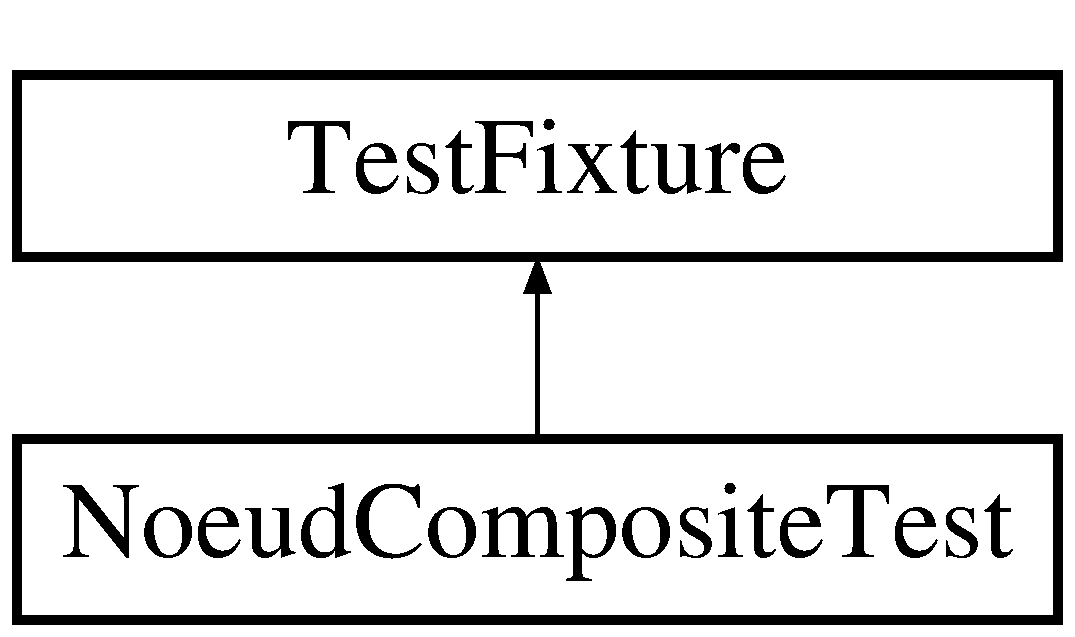
\includegraphics[height=2.000000cm]{class_noeud_composite_test}
\end{center}
\end{figure}
\subsection*{Fonctions membres publiques}
\begin{DoxyCompactItemize}
\item 
void \hyperlink{group__inf2990_gac580ba74910c8d4e8476ce2f4e1930a2}{set\-Up} ()
\begin{DoxyCompactList}\small\item\em Traitement à effectuer pour initialiser cette suite de tests. \end{DoxyCompactList}\item 
void \hyperlink{group__inf2990_gaab8590913d1e0ce48d52ca2875c12c92}{tear\-Down} ()
\begin{DoxyCompactList}\small\item\em Traitement à effectuer pour 'finaliser' cette suite de tests. \end{DoxyCompactList}\item 
void \hyperlink{group__inf2990_gae6e5ecfa0bfef3aa50bbfe4b082821e9}{test\-Obtenir\-Nombre\-Enfants} ()
\begin{DoxyCompactList}\small\item\em Cas de test\-: obtenir le nombre d'enfants. \end{DoxyCompactList}\item 
void \hyperlink{group__inf2990_ga5e667d5f1bc2bf30fe013e5a630d95d5}{test\-Vider} ()
\begin{DoxyCompactList}\small\item\em Cas de test\-: vider le noeud composite (supprimer tous ses enfants) \end{DoxyCompactList}\item 
void \hyperlink{group__inf2990_ga2f7f5a6ba30a148469a30a8c32a8690c}{test\-Effacer} ()
\begin{DoxyCompactList}\small\item\em Cas de test\-: effacer les noeuds enfants. \end{DoxyCompactList}\item 
void \hyperlink{group__inf2990_ga9dc8155dc795120e1d6abfbbee81161b}{test\-Effacer\-Selection} ()
\begin{DoxyCompactList}\small\item\em Cas de test\-: effacer les noeuds enfants sélectionnés. \end{DoxyCompactList}\item 
void \hyperlink{group__inf2990_ga684b84f99cf5a559386a96b8c4468683}{test\-Chercher} ()
\begin{DoxyCompactList}\small\item\em Cas de test\-: rechercher un noeud enfant. \end{DoxyCompactList}\item 
void \hyperlink{group__inf2990_gaaeb7bf3f97cb196df2398cdf1a639469}{test\-Ajouter} ()
\begin{DoxyCompactList}\small\item\em Cas de test\-: ajouter un noeud enfant. \end{DoxyCompactList}\item 
\hypertarget{group__inf2990_ga585be1924a9bfe61c2ee7bf91491695a}{void \hyperlink{group__inf2990_ga585be1924a9bfe61c2ee7bf91491695a}{test\-Selectionner\-Tout} ()}\label{group__inf2990_ga585be1924a9bfe61c2ee7bf91491695a}

\begin{DoxyCompactList}\small\item\em Cas de test\-: selectionner tous les enfants. \end{DoxyCompactList}\end{DoxyCompactItemize}


\subsection{Description détaillée}
Classe de test cppunit pour tester le bon fonctionnement des méthodes de la classe \hyperlink{class_noeud_composite}{Noeud\-Composite}. 

\begin{DoxyAuthor}{Auteur}
I\-N\-F2990-\/\-A15-\/01 
\end{DoxyAuthor}
\begin{DoxyDate}{Date}
2015-\/11-\/10 
\end{DoxyDate}


La documentation de cette classe a été générée à partir des fichiers suivants \-:\begin{DoxyCompactItemize}
\item 
C\-:/\-Users/saron/\-Documents/inf2990-\/01/\-Sources/\-D\-L\-L/\-Tests/\hyperlink{_noeud_composite_test_8h}{Noeud\-Composite\-Test.\-h}\item 
C\-:/\-Users/saron/\-Documents/inf2990-\/01/\-Sources/\-D\-L\-L/\-Tests/\hyperlink{_noeud_composite_test_8cpp}{Noeud\-Composite\-Test.\-cpp}\end{DoxyCompactItemize}

\hypertarget{class_noeud_cone_cube}{\section{Référence de la classe Noeud\-Cone\-Cube}
\label{class_noeud_cone_cube}\index{Noeud\-Cone\-Cube@{Noeud\-Cone\-Cube}}
}


Classe qui représente un exemple de noeud de l'arbre de rendu.  




{\ttfamily \#include $<$Noeud\-Cone\-Cube.\-h$>$}

Graphe d'héritage de Noeud\-Cone\-Cube\-:\begin{figure}[H]
\begin{center}
\leavevmode
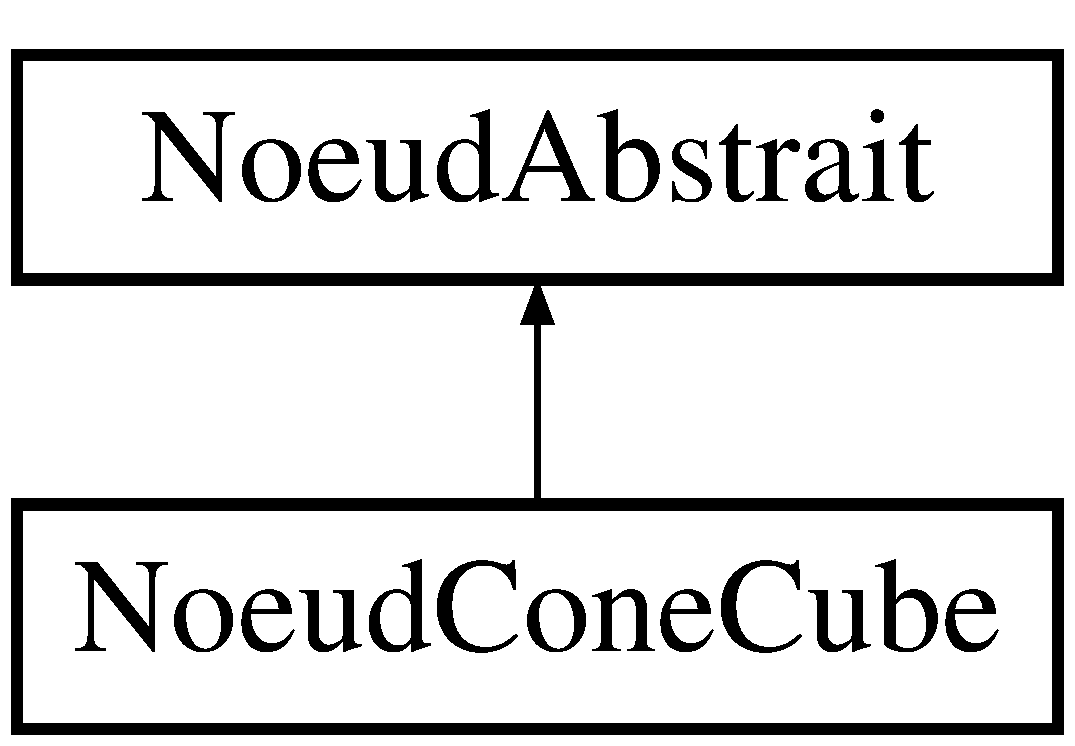
\includegraphics[height=2.000000cm]{class_noeud_cone_cube}
\end{center}
\end{figure}
\subsection*{Fonctions membres publiques}
\begin{DoxyCompactItemize}
\item 
\hyperlink{group__inf2990_ga6f0bcd8b494e8aa6f3a8dad78bad2c0f}{Noeud\-Cone\-Cube} (const std\-::string \&type\-Noeud)
\begin{DoxyCompactList}\small\item\em Constructeur à partir du type du noeud. \end{DoxyCompactList}\item 
\hyperlink{group__inf2990_ga8db4b36c3469001f7dcfab23debe7d2f}{$\sim$\-Noeud\-Cone\-Cube} ()
\begin{DoxyCompactList}\small\item\em Destructeur. \end{DoxyCompactList}\item 
virtual void \hyperlink{group__inf2990_ga4b1f68c409f0b1c5eabd0be7822a36d2}{afficher\-Concret} () const 
\begin{DoxyCompactList}\small\item\em Affiche le cube. \end{DoxyCompactList}\item 
\hypertarget{group__inf2990_ga3472a200d45ce3cdff72d72921807b21}{virtual void \hyperlink{group__inf2990_ga3472a200d45ce3cdff72d72921807b21}{animer} (float temps)}\label{group__inf2990_ga3472a200d45ce3cdff72d72921807b21}

\begin{DoxyCompactList}\small\item\em Effectue l'animation du cube. \end{DoxyCompactList}\item 
\hypertarget{class_noeud_cone_cube_a057b05f07c3aef977e295b519969ae04}{void {\bfseries accept} (\hyperlink{class_tool}{Tool} \&visitor) override}\label{class_noeud_cone_cube_a057b05f07c3aef977e295b519969ae04}

\end{DoxyCompactItemize}
\subsection*{Membres hérités additionnels}


\subsection{Description détaillée}
Classe qui représente un exemple de noeud de l'arbre de rendu. 

\begin{DoxyAuthor}{Auteur}
Julien Gascon-\/\-Samson 
\end{DoxyAuthor}
\begin{DoxyDate}{Date}
2011-\/05-\/19 
\end{DoxyDate}


La documentation de cette classe a été générée à partir des fichiers suivants \-:\begin{DoxyCompactItemize}
\item 
C\-:/\-Users/saron/\-Documents/inf2990-\/01/\-Sources/\-D\-L\-L/\-Arbre/\-Noeuds/\hyperlink{_noeud_cone_cube_8h}{Noeud\-Cone\-Cube.\-h}\item 
C\-:/\-Users/saron/\-Documents/inf2990-\/01/\-Sources/\-D\-L\-L/\-Arbre/\-Noeuds/\hyperlink{_noeud_cone_cube_8cpp}{Noeud\-Cone\-Cube.\-cpp}\end{DoxyCompactItemize}

\hypertarget{class_noeud_cylindre}{\section{Référence de la classe Noeud\-Cylindre}
\label{class_noeud_cylindre}\index{Noeud\-Cylindre@{Noeud\-Cylindre}}
}


Classe qui représente le noeud du cylindre dans l'arbre de rendu.  




{\ttfamily \#include $<$Noeud\-Cylindre.\-h$>$}

Graphe d'héritage de Noeud\-Cylindre\-:\begin{figure}[H]
\begin{center}
\leavevmode
\includegraphics[height=2.000000cm]{class_noeud_cylindre}
\end{center}
\end{figure}
\subsection*{Fonctions membres publiques}
{\bf }\par
\begin{DoxyCompactItemize}
\item 
\hyperlink{class_noeud_cylindre_aee7f35b6d758ac40b96daadf526f4504}{Noeud\-Cylindre} (const std\-::string \&type\-Noeud)
\begin{DoxyCompactList}\small\item\em Constructeur à partir du type du noeud. \end{DoxyCompactList}\item 
\hyperlink{class_noeud_cylindre_aa08fe15b1f926c8d651fcd467d3cb36a}{$\sim$\-Noeud\-Cylindre} ()
\begin{DoxyCompactList}\small\item\em Destructeur. \end{DoxyCompactList}\item 
virtual void \hyperlink{class_noeud_cylindre_a24bd5b287091cdecdd250ebb83594551}{afficher\-Concret} () const 
\begin{DoxyCompactList}\small\item\em Affiche la table. \end{DoxyCompactList}\item 
bool \hyperlink{class_noeud_cylindre_a524d454765b791a68d42e10254e58885}{click\-Hit} (glm\-::dvec3 point) override
\begin{DoxyCompactList}\small\item\em Si le click est sur le cylindre. \end{DoxyCompactList}\item 
bool \hyperlink{class_noeud_cylindre_a461dfbf53728711e290d14db7464f5f9}{click\-Hit} (glm\-::ivec2 debut, glm\-::ivec2 fin) override
\begin{DoxyCompactList}\small\item\em Si le click est sur le cylindre. \end{DoxyCompactList}\item 
void \hyperlink{class_noeud_cylindre_a37f3266147e98c0dd312ac674d88e9b4}{set\-Scale} (const glm\-::fvec3 scale) override
\item 
void \hyperlink{class_noeud_cylindre_a108b067e7817f5c83ca66643bb67769b}{accept} (\hyperlink{class_tool}{Tool} \&visitor) override
\begin{DoxyCompactList}\small\item\em Accepte un visiteur Outils. \end{DoxyCompactList}\end{DoxyCompactItemize}

\subsection*{Membres hérités additionnels}


\subsection{Description détaillée}
Classe qui représente le noeud du cylindre dans l'arbre de rendu. 

by \-: I\-N\-F2990-\/\-A15-\/01 \begin{DoxyDate}{Date}
2015-\/09-\/14
\end{DoxyDate}
\begin{DoxyAuthor}{Auteur}
Julien Gascon-\/\-Samson 
\end{DoxyAuthor}
\begin{DoxyDate}{Date}
2011-\/05-\/19 
\end{DoxyDate}


\subsection{Documentation des constructeurs et destructeur}
\hypertarget{class_noeud_cylindre_aee7f35b6d758ac40b96daadf526f4504}{\index{Noeud\-Cylindre@{Noeud\-Cylindre}!Noeud\-Cylindre@{Noeud\-Cylindre}}
\index{Noeud\-Cylindre@{Noeud\-Cylindre}!NoeudCylindre@{Noeud\-Cylindre}}
\subsubsection[{Noeud\-Cylindre}]{\setlength{\rightskip}{0pt plus 5cm}Noeud\-Cylindre\-::\-Noeud\-Cylindre (
\begin{DoxyParamCaption}
\item[{const std\-::string \&}]{type\-Noeud}
\end{DoxyParamCaption}
)}}\label{class_noeud_cylindre_aee7f35b6d758ac40b96daadf526f4504}


Constructeur à partir du type du noeud. 

Ce constructeur ne fait qu'appeler la version de la classe et base et donner des valeurs par défaut aux variables membres.


\begin{DoxyParams}[1]{Paramètres}
\mbox{\tt in}  & {\em type\-Noeud} & \-: Le type du noeud.\\
\hline
\end{DoxyParams}
\begin{DoxyReturn}{Renvoie}
Aucune (constructeur). 
\end{DoxyReturn}
\hypertarget{class_noeud_cylindre_aa08fe15b1f926c8d651fcd467d3cb36a}{\index{Noeud\-Cylindre@{Noeud\-Cylindre}!$\sim$\-Noeud\-Cylindre@{$\sim$\-Noeud\-Cylindre}}
\index{$\sim$\-Noeud\-Cylindre@{$\sim$\-Noeud\-Cylindre}!NoeudCylindre@{Noeud\-Cylindre}}
\subsubsection[{$\sim$\-Noeud\-Cylindre}]{\setlength{\rightskip}{0pt plus 5cm}Noeud\-Cylindre\-::$\sim$\-Noeud\-Cylindre (
\begin{DoxyParamCaption}
{}
\end{DoxyParamCaption}
)}}\label{class_noeud_cylindre_aa08fe15b1f926c8d651fcd467d3cb36a}


Destructeur. 

Ce destructeur désallouee la liste d'affichage du cube.

\begin{DoxyReturn}{Renvoie}
Aucune (destructeur). 
\end{DoxyReturn}


\subsection{Documentation des fonctions membres}
\hypertarget{class_noeud_cylindre_a108b067e7817f5c83ca66643bb67769b}{\index{Noeud\-Cylindre@{Noeud\-Cylindre}!accept@{accept}}
\index{accept@{accept}!NoeudCylindre@{Noeud\-Cylindre}}
\subsubsection[{accept}]{\setlength{\rightskip}{0pt plus 5cm}void Noeud\-Cylindre\-::accept (
\begin{DoxyParamCaption}
\item[{{\bf Tool} \&}]{visitor}
\end{DoxyParamCaption}
)\hspace{0.3cm}{\ttfamily [override]}, {\ttfamily [virtual]}}}\label{class_noeud_cylindre_a108b067e7817f5c83ca66643bb67769b}


Accepte un visiteur Outils. 

Cette fonction accepte un visiteur, et le bon visiteur.


\begin{DoxyParams}[1]{Paramètres}
\mbox{\tt in}  & {\em visitor} & \-: Le visiteur qui intervenient sur le noeud\\
\hline
\end{DoxyParams}
\begin{DoxyReturn}{Renvoie}
Aucune. 
\end{DoxyReturn}


Implémente \hyperlink{class_noeud_abstrait}{Noeud\-Abstrait}.

\hypertarget{class_noeud_cylindre_a24bd5b287091cdecdd250ebb83594551}{\index{Noeud\-Cylindre@{Noeud\-Cylindre}!afficher\-Concret@{afficher\-Concret}}
\index{afficher\-Concret@{afficher\-Concret}!NoeudCylindre@{Noeud\-Cylindre}}
\subsubsection[{afficher\-Concret}]{\setlength{\rightskip}{0pt plus 5cm}void Noeud\-Cylindre\-::afficher\-Concret (
\begin{DoxyParamCaption}
{}
\end{DoxyParamCaption}
) const\hspace{0.3cm}{\ttfamily [virtual]}}}\label{class_noeud_cylindre_a24bd5b287091cdecdd250ebb83594551}


Affiche la table. 

Cette fonction effectue le véritable rendu de l'objet.

\begin{DoxyReturn}{Renvoie}
Aucune. 
\end{DoxyReturn}


Réimplémentée à partir de \hyperlink{group__inf2990_ga330df455c8b08440d3c8e64d0a480391}{Noeud\-Abstrait}.

\hypertarget{class_noeud_cylindre_a524d454765b791a68d42e10254e58885}{\index{Noeud\-Cylindre@{Noeud\-Cylindre}!click\-Hit@{click\-Hit}}
\index{click\-Hit@{click\-Hit}!NoeudCylindre@{Noeud\-Cylindre}}
\subsubsection[{click\-Hit}]{\setlength{\rightskip}{0pt plus 5cm}bool Noeud\-Cylindre\-::click\-Hit (
\begin{DoxyParamCaption}
\item[{glm\-::dvec3}]{point}
\end{DoxyParamCaption}
)\hspace{0.3cm}{\ttfamily [override]}, {\ttfamily [virtual]}}}\label{class_noeud_cylindre_a524d454765b791a68d42e10254e58885}


Si le click est sur le cylindre. 

bool Noeud\-Cylindre\-::click\-Hit(\-G\-Ldouble x, G\-Ldouble y, G\-Ldouble z)

Vérifie si le clic de souris touche le modèle du noeud


\begin{DoxyParams}[1]{Paramètres}
\mbox{\tt in}  & {\em x,y,z} & \-: Les coordonnées du clic\\
\hline
\end{DoxyParams}
\begin{DoxyReturn}{Renvoie}
Aucune. 
\end{DoxyReturn}


Réimplémentée à partir de \hyperlink{class_noeud_abstrait}{Noeud\-Abstrait}.

\hypertarget{class_noeud_cylindre_a461dfbf53728711e290d14db7464f5f9}{\index{Noeud\-Cylindre@{Noeud\-Cylindre}!click\-Hit@{click\-Hit}}
\index{click\-Hit@{click\-Hit}!NoeudCylindre@{Noeud\-Cylindre}}
\subsubsection[{click\-Hit}]{\setlength{\rightskip}{0pt plus 5cm}bool Noeud\-Cylindre\-::click\-Hit (
\begin{DoxyParamCaption}
\item[{glm\-::ivec2}]{debut, }
\item[{glm\-::ivec2}]{fin}
\end{DoxyParamCaption}
)\hspace{0.3cm}{\ttfamily [override]}, {\ttfamily [virtual]}}}\label{class_noeud_cylindre_a461dfbf53728711e290d14db7464f5f9}


Si le click est sur le cylindre. 

bool \hyperlink{class_noeud_cylindre_a524d454765b791a68d42e10254e58885}{Noeud\-Cylindre\-::click\-Hit}((glm\-::ivec2 debut, glm\-::ivec2 fin)

Vérifie si le noeud est à l'interieur du rectangle


\begin{DoxyParams}[1]{Paramètres}
\mbox{\tt in}  & {\em x,y,z} & \-: Les coordonnées du clic\\
\hline
\end{DoxyParams}
\begin{DoxyReturn}{Renvoie}
Aucune. 
\end{DoxyReturn}


Réimplémentée à partir de \hyperlink{group__inf2990_gad1d1a9c6adcedfcd5eda6c6d4e67a50f}{Noeud\-Abstrait}.

\hypertarget{class_noeud_cylindre_a37f3266147e98c0dd312ac674d88e9b4}{\index{Noeud\-Cylindre@{Noeud\-Cylindre}!set\-Scale@{set\-Scale}}
\index{set\-Scale@{set\-Scale}!NoeudCylindre@{Noeud\-Cylindre}}
\subsubsection[{set\-Scale}]{\setlength{\rightskip}{0pt plus 5cm}void Noeud\-Cylindre\-::set\-Scale (
\begin{DoxyParamCaption}
\item[{const glm\-::fvec3}]{scale}
\end{DoxyParamCaption}
)\hspace{0.3cm}{\ttfamily [inline]}, {\ttfamily [override]}, {\ttfamily [virtual]}}}\label{class_noeud_cylindre_a37f3266147e98c0dd312ac674d88e9b4}
Cette fonction permet d'assigner l'échelle du noeud.


\begin{DoxyParams}{Paramètres}
{\em angle\-Initial} & \-: L'échelle.\\
\hline
\end{DoxyParams}
\begin{DoxyReturn}{Renvoie}
Aucune 
\end{DoxyReturn}


Réimplémentée à partir de \hyperlink{group__inf2990_gaef8fd99796f85418adac496160a3350b}{Noeud\-Abstrait}.



La documentation de cette classe a été générée à partir des fichiers suivants \-:\begin{DoxyCompactItemize}
\item 
C\-:/\-Users/saron/\-Documents/inf2990-\/01/\-Sources/\-D\-L\-L/\-Arbre/\-Noeuds/\hyperlink{_noeud_cylindre_8h}{Noeud\-Cylindre.\-h}\item 
C\-:/\-Users/saron/\-Documents/inf2990-\/01/\-Sources/\-D\-L\-L/\-Arbre/\-Noeuds/\hyperlink{_noeud_cylindre_8cpp}{Noeud\-Cylindre.\-cpp}\end{DoxyCompactItemize}

\hypertarget{class_noeud_depart}{}\section{Noeud\+Depart Class Reference}
\label{class_noeud_depart}\index{Noeud\+Depart@{Noeud\+Depart}}


Classe qui représente le point de départ dans l\textquotesingle{}arbre de rendu.  




{\ttfamily \#include $<$Noeud\+Depart.\+h$>$}

Inheritance diagram for Noeud\+Depart\+:\begin{figure}[H]
\begin{center}
\leavevmode
\includegraphics[height=2.000000cm]{class_noeud_depart}
\end{center}
\end{figure}
\subsection*{Public Member Functions}
\begin{DoxyCompactItemize}
\item 
\hypertarget{class_noeud_depart_a6a1abd18717d2072edebff29d5d21995}{}\hyperlink{class_noeud_depart_a6a1abd18717d2072edebff29d5d21995}{$\sim$\+Noeud\+Depart} ()=default\label{class_noeud_depart_a6a1abd18717d2072edebff29d5d21995}

\begin{DoxyCompactList}\small\item\em Destructeur. \end{DoxyCompactList}\item 
\hypertarget{class_noeud_depart_ac02ac846dec4dd15b5ac2656c0907134}{}void \hyperlink{class_noeud_depart_ac02ac846dec4dd15b5ac2656c0907134}{set\+Scale} (const glm\+::fvec3 scale) override\label{class_noeud_depart_ac02ac846dec4dd15b5ac2656c0907134}

\begin{DoxyCompactList}\small\item\em On ne peux pas changer le scale du spawn. \end{DoxyCompactList}\item 
\hypertarget{class_noeud_depart_ac2889c3bb1f8f3d373261a93ea455f70}{}void \hyperlink{class_noeud_depart_ac2889c3bb1f8f3d373261a93ea455f70}{set\+Scale\+Initial} (const glm\+::fvec3 scale) override\label{class_noeud_depart_ac2889c3bb1f8f3d373261a93ea455f70}

\begin{DoxyCompactList}\small\item\em On ne peux pas changer le scale du spawn. \end{DoxyCompactList}\end{DoxyCompactItemize}
{\bf }\par
\begin{DoxyCompactItemize}
\item 
\hyperlink{class_noeud_depart_a003d2fbed3f4e142a9187a8152a4663d}{Noeud\+Depart} (const std\+::string \&type\+Noeud)
\begin{DoxyCompactList}\small\item\em Constructeur à partir du type du noeud. \end{DoxyCompactList}\item 
void \hyperlink{class_noeud_depart_a1335eaf607cc753bf818aded966144fe}{afficher\+Concret} () const  override
\begin{DoxyCompactList}\small\item\em Affiche la table. \end{DoxyCompactList}\item 
void \hyperlink{class_noeud_depart_a5c105e25f600256c8933f70e07608413}{accept} (\hyperlink{class_tool}{Tool} \&visitor) override
\begin{DoxyCompactList}\small\item\em Accepte un visiteur Outils. \end{DoxyCompactList}\item 
\hypertarget{class_noeud_depart_a5bbaf0ff7096cff7e73f5054014b723e}{}bool \hyperlink{class_noeud_depart_a5bbaf0ff7096cff7e73f5054014b723e}{click\+Hit} (glm\+::dvec3 point) override\label{class_noeud_depart_a5bbaf0ff7096cff7e73f5054014b723e}

\begin{DoxyCompactList}\small\item\em Si le click est sur le spawn. \end{DoxyCompactList}\item 
\hypertarget{class_noeud_depart_a2dfe8b7300b4f1933993d44754e8f53f}{}bool \hyperlink{class_noeud_depart_a2dfe8b7300b4f1933993d44754e8f53f}{click\+Hit} (glm\+::ivec2 debut, glm\+::ivec2 fin) override\label{class_noeud_depart_a2dfe8b7300b4f1933993d44754e8f53f}

\begin{DoxyCompactList}\small\item\em Si le click est sur le spawn. \end{DoxyCompactList}\end{DoxyCompactItemize}

\subsection*{Additional Inherited Members}


\subsection{Detailed Description}
Classe qui représente le point de départ dans l\textquotesingle{}arbre de rendu. 

\begin{DoxyAuthor}{Author}
I\+N\+F2990-\/\+A15-\/01 
\end{DoxyAuthor}
\begin{DoxyDate}{Date}
2015-\/09-\/18 
\end{DoxyDate}


\subsection{Constructor \& Destructor Documentation}
\hypertarget{class_noeud_depart_a003d2fbed3f4e142a9187a8152a4663d}{}\index{Noeud\+Depart@{Noeud\+Depart}!Noeud\+Depart@{Noeud\+Depart}}
\index{Noeud\+Depart@{Noeud\+Depart}!Noeud\+Depart@{Noeud\+Depart}}
\subsubsection[{Noeud\+Depart(const std\+::string \&type\+Noeud)}]{\setlength{\rightskip}{0pt plus 5cm}Noeud\+Depart\+::\+Noeud\+Depart (
\begin{DoxyParamCaption}
\item[{const std\+::string \&}]{type\+Noeud}
\end{DoxyParamCaption}
)}\label{class_noeud_depart_a003d2fbed3f4e142a9187a8152a4663d}


Constructeur à partir du type du noeud. 

Ce constructeur ne fait qu\textquotesingle{}appeler la version de la classe de base et donner des valeurs par défaut aux variables membres.


\begin{DoxyParams}[1]{Parameters}
\mbox{\tt in}  & {\em type\+Noeud} & \+: Le type du noeud.\\
\hline
\end{DoxyParams}
\begin{DoxyReturn}{Returns}
Aucune (constructeur). 
\end{DoxyReturn}


\subsection{Member Function Documentation}
\hypertarget{class_noeud_depart_a5c105e25f600256c8933f70e07608413}{}\index{Noeud\+Depart@{Noeud\+Depart}!accept@{accept}}
\index{accept@{accept}!Noeud\+Depart@{Noeud\+Depart}}
\subsubsection[{accept(\+Tool \&visitor) override}]{\setlength{\rightskip}{0pt plus 5cm}void Noeud\+Depart\+::accept (
\begin{DoxyParamCaption}
\item[{{\bf Tool} \&}]{visitor}
\end{DoxyParamCaption}
)\hspace{0.3cm}{\ttfamily [override]}, {\ttfamily [virtual]}}\label{class_noeud_depart_a5c105e25f600256c8933f70e07608413}


Accepte un visiteur Outils. 

Cette fonction accepte un visiteur, et le bon visiteur.


\begin{DoxyParams}[1]{Parameters}
\mbox{\tt in}  & {\em visitor} & \+: Le visiteur qui intervenient sur le noeud\\
\hline
\end{DoxyParams}
\begin{DoxyReturn}{Returns}
Aucune. 
\end{DoxyReturn}


Implements \hyperlink{class_noeud_abstrait}{Noeud\+Abstrait}.

\hypertarget{class_noeud_depart_a1335eaf607cc753bf818aded966144fe}{}\index{Noeud\+Depart@{Noeud\+Depart}!afficher\+Concret@{afficher\+Concret}}
\index{afficher\+Concret@{afficher\+Concret}!Noeud\+Depart@{Noeud\+Depart}}
\subsubsection[{afficher\+Concret() const  override}]{\setlength{\rightskip}{0pt plus 5cm}void Noeud\+Depart\+::afficher\+Concret (
\begin{DoxyParamCaption}
{}
\end{DoxyParamCaption}
) const\hspace{0.3cm}{\ttfamily [override]}, {\ttfamily [virtual]}}\label{class_noeud_depart_a1335eaf607cc753bf818aded966144fe}


Affiche la table. 

Cette fonction effectue le véritable rendu de l\textquotesingle{}objet.

\begin{DoxyReturn}{Returns}
Aucune. 
\end{DoxyReturn}


Reimplemented from \hyperlink{group__inf2990_ga330df455c8b08440d3c8e64d0a480391}{Noeud\+Abstrait}.



The documentation for this class was generated from the following files\+:\begin{DoxyCompactItemize}
\item 
C\+:/\+Users/\+Louis/workspace/inf2990-\/01/\+Sources/\+D\+L\+L/\+Arbre/\+Noeuds/\hyperlink{_noeud_depart_8h}{Noeud\+Depart.\+h}\item 
C\+:/\+Users/\+Louis/workspace/inf2990-\/01/\+Sources/\+D\+L\+L/\+Arbre/\+Noeuds/\hyperlink{_noeud_depart_8cpp}{Noeud\+Depart.\+cpp}\end{DoxyCompactItemize}

\hypertarget{class_noeud_ligne_composite}{}\section{Noeud\+Ligne\+Composite Class Reference}
\label{class_noeud_ligne_composite}\index{Noeud\+Ligne\+Composite@{Noeud\+Ligne\+Composite}}


Classe qui représente le noeud de la table dans l\textquotesingle{}arbre de rendu.  




{\ttfamily \#include $<$Noeud\+Ligne\+Composite.\+h$>$}

Inheritance diagram for Noeud\+Ligne\+Composite\+:\begin{figure}[H]
\begin{center}
\leavevmode
\includegraphics[height=3.000000cm]{class_noeud_ligne_composite}
\end{center}
\end{figure}
\subsection*{Public Member Functions}
{\bf }\par
\begin{DoxyCompactItemize}
\item 
\hyperlink{class_noeud_ligne_composite_af9846268635cbb0331feab18575c2607}{Noeud\+Ligne\+Composite} (const std\+::string \&type\+Noeud)
\begin{DoxyCompactList}\small\item\em Constructeur à partir du type du noeud. \end{DoxyCompactList}\item 
\hyperlink{class_noeud_ligne_composite_a400904537333bb2ae7e462ced349bdd2}{$\sim$\+Noeud\+Ligne\+Composite} ()
\begin{DoxyCompactList}\small\item\em Destructeur. \end{DoxyCompactList}\item 
virtual void \hyperlink{class_noeud_ligne_composite_a24738e9ba75c1b0d69e5a99edcba1682}{afficher\+Concret} () const 
\begin{DoxyCompactList}\small\item\em Affiche la ligne. \end{DoxyCompactList}\item 
bool \hyperlink{class_noeud_ligne_composite_a2b7f3bf28018fc6c6616b539dc342524}{click\+Hit} (G\+Ldouble x, G\+Ldouble y, G\+Ldouble z) override
\begin{DoxyCompactList}\small\item\em Effectue l\textquotesingle{}animation de la ligne. \end{DoxyCompactList}\end{DoxyCompactItemize}

\subsection*{Additional Inherited Members}


\subsection{Detailed Description}
Classe qui représente le noeud de la table dans l\textquotesingle{}arbre de rendu. 

by \+: Barouche Sabrina \begin{DoxyDate}{Date}
2015-\/09-\/14
\end{DoxyDate}
\begin{DoxyAuthor}{Author}
Julien Gascon-\/\+Samson 
\end{DoxyAuthor}
\begin{DoxyDate}{Date}
2011-\/05-\/19 
\end{DoxyDate}


\subsection{Constructor \& Destructor Documentation}
\hypertarget{class_noeud_ligne_composite_af9846268635cbb0331feab18575c2607}{}\index{Noeud\+Ligne\+Composite@{Noeud\+Ligne\+Composite}!Noeud\+Ligne\+Composite@{Noeud\+Ligne\+Composite}}
\index{Noeud\+Ligne\+Composite@{Noeud\+Ligne\+Composite}!Noeud\+Ligne\+Composite@{Noeud\+Ligne\+Composite}}
\subsubsection[{Noeud\+Ligne\+Composite(const std\+::string \&type\+Noeud)}]{\setlength{\rightskip}{0pt plus 5cm}Noeud\+Ligne\+Composite\+::\+Noeud\+Ligne\+Composite (
\begin{DoxyParamCaption}
\item[{const std\+::string \&}]{type\+Noeud}
\end{DoxyParamCaption}
)}\label{class_noeud_ligne_composite_af9846268635cbb0331feab18575c2607}


Constructeur à partir du type du noeud. 

Ce constructeur ne fait qu\textquotesingle{}appeler la version de la classe et base et donner des valeurs par défaut aux variables membres.


\begin{DoxyParams}[1]{Parameters}
\mbox{\tt in}  & {\em type\+Noeud} & \+: Le type du noeud.\\
\hline
\end{DoxyParams}
\begin{DoxyReturn}{Returns}
Aucune (constructeur). 
\end{DoxyReturn}
\hypertarget{class_noeud_ligne_composite_a400904537333bb2ae7e462ced349bdd2}{}\index{Noeud\+Ligne\+Composite@{Noeud\+Ligne\+Composite}!````~Noeud\+Ligne\+Composite@{$\sim$\+Noeud\+Ligne\+Composite}}
\index{````~Noeud\+Ligne\+Composite@{$\sim$\+Noeud\+Ligne\+Composite}!Noeud\+Ligne\+Composite@{Noeud\+Ligne\+Composite}}
\subsubsection[{$\sim$\+Noeud\+Ligne\+Composite()}]{\setlength{\rightskip}{0pt plus 5cm}Noeud\+Ligne\+Composite\+::$\sim$\+Noeud\+Ligne\+Composite (
\begin{DoxyParamCaption}
{}
\end{DoxyParamCaption}
)}\label{class_noeud_ligne_composite_a400904537333bb2ae7e462ced349bdd2}


Destructeur. 

Ce destructeur désallouee la liste d\textquotesingle{}affichage du la ligne.

\begin{DoxyReturn}{Returns}
Aucune (destructeur). 
\end{DoxyReturn}


\subsection{Member Function Documentation}
\hypertarget{class_noeud_ligne_composite_a24738e9ba75c1b0d69e5a99edcba1682}{}\index{Noeud\+Ligne\+Composite@{Noeud\+Ligne\+Composite}!afficher\+Concret@{afficher\+Concret}}
\index{afficher\+Concret@{afficher\+Concret}!Noeud\+Ligne\+Composite@{Noeud\+Ligne\+Composite}}
\subsubsection[{afficher\+Concret() const }]{\setlength{\rightskip}{0pt plus 5cm}void Noeud\+Ligne\+Composite\+::afficher\+Concret (
\begin{DoxyParamCaption}
{}
\end{DoxyParamCaption}
) const\hspace{0.3cm}{\ttfamily [virtual]}}\label{class_noeud_ligne_composite_a24738e9ba75c1b0d69e5a99edcba1682}


Affiche la ligne. 

Cette fonction effectue le véritable rendu de l\textquotesingle{}objet.

\begin{DoxyReturn}{Returns}
Aucune. 
\end{DoxyReturn}


Reimplemented from \hyperlink{group__inf2990_gaed396ee8ea0396e4a9cf56b69151204b}{Noeud\+Composite}.

\hypertarget{class_noeud_ligne_composite_a2b7f3bf28018fc6c6616b539dc342524}{}\index{Noeud\+Ligne\+Composite@{Noeud\+Ligne\+Composite}!click\+Hit@{click\+Hit}}
\index{click\+Hit@{click\+Hit}!Noeud\+Ligne\+Composite@{Noeud\+Ligne\+Composite}}
\subsubsection[{click\+Hit(\+G\+Ldouble x, G\+Ldouble y, G\+Ldouble z) override}]{\setlength{\rightskip}{0pt plus 5cm}bool Noeud\+Ligne\+Composite\+::click\+Hit (
\begin{DoxyParamCaption}
\item[{G\+Ldouble}]{x, }
\item[{G\+Ldouble}]{y, }
\item[{G\+Ldouble}]{z}
\end{DoxyParamCaption}
)\hspace{0.3cm}{\ttfamily [override]}, {\ttfamily [virtual]}}\label{class_noeud_ligne_composite_a2b7f3bf28018fc6c6616b539dc342524}


Effectue l\textquotesingle{}animation de la ligne. 

Vérifie si le clic de souris touche le modèle du noeud


\begin{DoxyParams}[1]{Parameters}
\mbox{\tt in}  & {\em x,y,z} & \+: Les coordonnées du clic\\
\hline
\end{DoxyParams}
\begin{DoxyReturn}{Returns}
Aucune. 
\end{DoxyReturn}


Reimplemented from \hyperlink{group__inf2990_ga2e40156a7ff6dd734c61de990db1bfe0}{Noeud\+Abstrait}.



The documentation for this class was generated from the following files\+:\begin{DoxyCompactItemize}
\item 
Sources/\+D\+L\+L/\+Arbre/\+Noeuds/Noeud\+Ligne\+Composite.\+h\item 
Sources/\+D\+L\+L/\+Arbre/\+Noeuds/Noeud\+Ligne\+Composite.\+cpp\end{DoxyCompactItemize}

\hypertarget{class_noeud_mur}{}\section{Noeud\+Mur Class Reference}
\label{class_noeud_mur}\index{Noeud\+Mur@{Noeud\+Mur}}


Classe qui représente le noeud du mur dans l\textquotesingle{}arbre de rendu.  




{\ttfamily \#include $<$Noeud\+Mur.\+h$>$}

Inheritance diagram for Noeud\+Mur\+:\begin{figure}[H]
\begin{center}
\leavevmode
\includegraphics[height=2.000000cm]{class_noeud_mur}
\end{center}
\end{figure}
\subsection*{Public Member Functions}
{\bf }\par
\begin{DoxyCompactItemize}
\item 
\hyperlink{class_noeud_mur_aeab2deec90548c0bdca5eb86beb629cf}{Noeud\+Mur} (const std\+::string \&type\+Noeud)
\begin{DoxyCompactList}\small\item\em Constructeur à partir du type du noeud. \end{DoxyCompactList}\item 
void \hyperlink{class_noeud_mur_a9f86d3ce3675f79abe879143e6dd4e8b}{update\+Creation} (glm\+::dvec3 cursor) override
\begin{DoxyCompactList}\small\item\em Deuxième étape de la construction. \end{DoxyCompactList}\item 
\hyperlink{class_noeud_mur_a169060e04a6423e7f025d475afd7d9ea}{$\sim$\+Noeud\+Mur} ()
\begin{DoxyCompactList}\small\item\em Destructeur. \end{DoxyCompactList}\item 
virtual void \hyperlink{class_noeud_mur_a521a3062875ea6ed1645485412a70c7b}{afficher\+Concret} () const 
\begin{DoxyCompactList}\small\item\em Affiche le mur. \end{DoxyCompactList}\item 
\hypertarget{class_noeud_mur_a267fe3fba8110e59fa76412f788ea8d1}{}void \hyperlink{class_noeud_mur_a267fe3fba8110e59fa76412f788ea8d1}{accept} (\hyperlink{class_tool}{Tool} \&visitor) override\label{class_noeud_mur_a267fe3fba8110e59fa76412f788ea8d1}

\begin{DoxyCompactList}\small\item\em Accepte un visiteur Outils. \end{DoxyCompactList}\end{DoxyCompactItemize}

\subsection*{Additional Inherited Members}


\subsection{Detailed Description}
Classe qui représente le noeud du mur dans l\textquotesingle{}arbre de rendu. 

by \+: Marc Lacharite-\/\+Laframboise \begin{DoxyDate}{Date}
2015-\/09-\/14
\end{DoxyDate}
\begin{DoxyAuthor}{Author}
Julien Gascon-\/\+Samson 
\end{DoxyAuthor}
\begin{DoxyDate}{Date}
2011-\/05-\/19 
\end{DoxyDate}


\subsection{Constructor \& Destructor Documentation}
\hypertarget{class_noeud_mur_aeab2deec90548c0bdca5eb86beb629cf}{}\index{Noeud\+Mur@{Noeud\+Mur}!Noeud\+Mur@{Noeud\+Mur}}
\index{Noeud\+Mur@{Noeud\+Mur}!Noeud\+Mur@{Noeud\+Mur}}
\subsubsection[{Noeud\+Mur(const std\+::string \&type\+Noeud)}]{\setlength{\rightskip}{0pt plus 5cm}Noeud\+Mur\+::\+Noeud\+Mur (
\begin{DoxyParamCaption}
\item[{const std\+::string \&}]{type\+Noeud}
\end{DoxyParamCaption}
)}\label{class_noeud_mur_aeab2deec90548c0bdca5eb86beb629cf}


Constructeur à partir du type du noeud. 

Ce constructeur ne fait qu\textquotesingle{}appeler la version de la classe de base et donner des valeurs par défaut aux variables membres.


\begin{DoxyParams}[1]{Parameters}
\mbox{\tt in}  & {\em type\+Noeud} & \+: Le type du noeud.\\
\hline
\end{DoxyParams}
\begin{DoxyReturn}{Returns}
Aucune (constructeur). 
\end{DoxyReturn}
\hypertarget{class_noeud_mur_a169060e04a6423e7f025d475afd7d9ea}{}\index{Noeud\+Mur@{Noeud\+Mur}!````~Noeud\+Mur@{$\sim$\+Noeud\+Mur}}
\index{````~Noeud\+Mur@{$\sim$\+Noeud\+Mur}!Noeud\+Mur@{Noeud\+Mur}}
\subsubsection[{$\sim$\+Noeud\+Mur()}]{\setlength{\rightskip}{0pt plus 5cm}Noeud\+Mur\+::$\sim$\+Noeud\+Mur (
\begin{DoxyParamCaption}
{}
\end{DoxyParamCaption}
)}\label{class_noeud_mur_a169060e04a6423e7f025d475afd7d9ea}


Destructeur. 

Ce destructeur désallouee la liste d\textquotesingle{}affichage du cube.

\begin{DoxyReturn}{Returns}
Aucune (destructeur). 
\end{DoxyReturn}


\subsection{Member Function Documentation}
\hypertarget{class_noeud_mur_a521a3062875ea6ed1645485412a70c7b}{}\index{Noeud\+Mur@{Noeud\+Mur}!afficher\+Concret@{afficher\+Concret}}
\index{afficher\+Concret@{afficher\+Concret}!Noeud\+Mur@{Noeud\+Mur}}
\subsubsection[{afficher\+Concret() const }]{\setlength{\rightskip}{0pt plus 5cm}void Noeud\+Mur\+::afficher\+Concret (
\begin{DoxyParamCaption}
{}
\end{DoxyParamCaption}
) const\hspace{0.3cm}{\ttfamily [virtual]}}\label{class_noeud_mur_a521a3062875ea6ed1645485412a70c7b}


Affiche le mur. 

Cette fonction effectue le véritable rendu de l\textquotesingle{}objet.

\begin{DoxyReturn}{Returns}
Aucune. 
\end{DoxyReturn}


Reimplemented from \hyperlink{group__inf2990_ga330df455c8b08440d3c8e64d0a480391}{Noeud\+Abstrait}.

\hypertarget{class_noeud_mur_a9f86d3ce3675f79abe879143e6dd4e8b}{}\index{Noeud\+Mur@{Noeud\+Mur}!update\+Creation@{update\+Creation}}
\index{update\+Creation@{update\+Creation}!Noeud\+Mur@{Noeud\+Mur}}
\subsubsection[{update\+Creation(glm\+::dvec3 cursor) override}]{\setlength{\rightskip}{0pt plus 5cm}void Noeud\+Mur\+::update\+Creation (
\begin{DoxyParamCaption}
\item[{glm\+::dvec3}]{cursor}
\end{DoxyParamCaption}
)\hspace{0.3cm}{\ttfamily [override]}, {\ttfamily [virtual]}}\label{class_noeud_mur_a9f86d3ce3675f79abe879143e6dd4e8b}


Deuxième étape de la construction. 

Dit au noeud de mettre à jour son affichage par rapport au curseur. Utilisé lors de la création d\textquotesingle{}un noeud en deux étapes (mur, ligne).


\begin{DoxyParams}[1]{Parameters}
\mbox{\tt in}  & {\em cursor} & \+: Les coordonnées du clic\\
\hline
\end{DoxyParams}
\begin{DoxyReturn}{Returns}
Aucune. 
\end{DoxyReturn}


Reimplemented from \hyperlink{group__inf2990_ga233fd4600812176c557bb94ea04da5c9}{Noeud\+Abstrait}.



The documentation for this class was generated from the following files\+:\begin{DoxyCompactItemize}
\item 
Sources/\+D\+L\+L/\+Arbre/\+Noeuds/\hyperlink{_noeud_mur_8h}{Noeud\+Mur.\+h}\item 
Sources/\+D\+L\+L/\+Arbre/\+Noeuds/\hyperlink{_noeud_mur_8cpp}{Noeud\+Mur.\+cpp}\end{DoxyCompactItemize}

\hypertarget{class_noeud_robot}{}\section{Noeud\+Robot Class Reference}
\label{class_noeud_robot}\index{Noeud\+Robot@{Noeud\+Robot}}


Classe qui représente le robot du premier projet intégrateur.  




{\ttfamily \#include $<$Noeud\+Robot.\+h$>$}

Inheritance diagram for Noeud\+Robot\+:\begin{figure}[H]
\begin{center}
\leavevmode
\includegraphics[height=3.000000cm]{class_noeud_robot}
\end{center}
\end{figure}
\subsection*{Public Member Functions}
\begin{DoxyCompactItemize}
\item 
\hyperlink{group__inf2990_ga147453ac7f72970d7d9bfe336998ad94}{Noeud\+Robot} (const std\+::string \&type\+Noeud)
\begin{DoxyCompactList}\small\item\em Constructeur à partir du type du noeud. \end{DoxyCompactList}\item 
\hyperlink{group__inf2990_ga5649710d151f0548d8a7a279aad4c655}{$\sim$\+Noeud\+Robot} ()
\begin{DoxyCompactList}\small\item\em Destructeur. \end{DoxyCompactList}\item 
virtual void \hyperlink{group__inf2990_gad63a8e09cc5ca8cc349f35e0901474e2}{afficher\+Concret} () const 
\begin{DoxyCompactList}\small\item\em Affiche le robot. \end{DoxyCompactList}\end{DoxyCompactItemize}
\subsection*{Additional Inherited Members}


\subsection{Detailed Description}
Classe qui représente le robot du premier projet intégrateur. 

\begin{DoxyAuthor}{Author}
Martin Paradis 
\end{DoxyAuthor}
\begin{DoxyDate}{Date}
2015-\/08-\/30 
\end{DoxyDate}


The documentation for this class was generated from the following files\+:\begin{DoxyCompactItemize}
\item 
Sources/\+D\+L\+L/\+Arbre/\+Noeuds/\hyperlink{_noeud_robot_8h}{Noeud\+Robot.\+h}\item 
Sources/\+D\+L\+L/\+Arbre/\+Noeuds/\hyperlink{_noeud_robot_8cpp}{Noeud\+Robot.\+cpp}\end{DoxyCompactItemize}

\hypertarget{class_noeud_segment_concret}{}\section{Noeud\+Segment\+Concret Class Reference}
\label{class_noeud_segment_concret}\index{Noeud\+Segment\+Concret@{Noeud\+Segment\+Concret}}


Classe qui représente le noeud d\textquotesingle{}un segment de ligne dans l\textquotesingle{}arbre de rendu.  




{\ttfamily \#include $<$Noeud\+Segment\+Concret.\+h$>$}

Inheritance diagram for Noeud\+Segment\+Concret\+:\begin{figure}[H]
\begin{center}
\leavevmode
\includegraphics[height=2.000000cm]{class_noeud_segment_concret}
\end{center}
\end{figure}
\subsection*{Public Member Functions}
{\bf }\par
\begin{DoxyCompactItemize}
\item 
\hyperlink{class_noeud_segment_concret_a5fa9b4c7e916ecba1afdee2b92b782d0}{Noeud\+Segment\+Concret} (const std\+::string \&type\+Noeud)
\begin{DoxyCompactList}\small\item\em Constructeur à partir du type du noeud. \end{DoxyCompactList}\item 
\hyperlink{class_noeud_segment_concret_a1b6277e30f5a24954bd38c915914887d}{$\sim$\+Noeud\+Segment\+Concret} ()
\begin{DoxyCompactList}\small\item\em Destructeur. \end{DoxyCompactList}\item 
virtual void \hyperlink{class_noeud_segment_concret_a755c965f09fe2ca3d148812fda08b5d6}{afficher\+Concret} () const 
\begin{DoxyCompactList}\small\item\em Affiche la segment. \end{DoxyCompactList}\item 
bool \hyperlink{class_noeud_segment_concret_a5aa1e10fe850cab0bb32290f9f228e9b}{click\+Hit} (G\+Ldouble x, G\+Ldouble y, G\+Ldouble z)
\begin{DoxyCompactList}\small\item\em Effectue l\textquotesingle{}animation du segment. \end{DoxyCompactList}\item 
bool \hyperlink{class_noeud_segment_concret_a6a98a44348fcd5fcccad77ffa48efc52}{click\+Hit} (glm\+::ivec2 debut, glm\+::ivec2 fin)
\item 
\hypertarget{class_noeud_segment_concret_a89f6362356646f3cc7d564aba168712d}{}void \hyperlink{class_noeud_segment_concret_a89f6362356646f3cc7d564aba168712d}{accept} (\hyperlink{class_tool}{Tool} \&visitor) override\label{class_noeud_segment_concret_a89f6362356646f3cc7d564aba168712d}

\begin{DoxyCompactList}\small\item\em Accepte un visiteur Outils. \end{DoxyCompactList}\end{DoxyCompactItemize}

\subsection*{Additional Inherited Members}


\subsection{Detailed Description}
Classe qui représente le noeud d\textquotesingle{}un segment de ligne dans l\textquotesingle{}arbre de rendu. 

\begin{DoxyAuthor}{Author}
I\+N\+F2990-\/\+A15-\/01 
\end{DoxyAuthor}
\begin{DoxyDate}{Date}
2015-\/09-\/18 
\end{DoxyDate}


\subsection{Constructor \& Destructor Documentation}
\hypertarget{class_noeud_segment_concret_a5fa9b4c7e916ecba1afdee2b92b782d0}{}\index{Noeud\+Segment\+Concret@{Noeud\+Segment\+Concret}!Noeud\+Segment\+Concret@{Noeud\+Segment\+Concret}}
\index{Noeud\+Segment\+Concret@{Noeud\+Segment\+Concret}!Noeud\+Segment\+Concret@{Noeud\+Segment\+Concret}}
\subsubsection[{Noeud\+Segment\+Concret(const std\+::string \&type\+Noeud)}]{\setlength{\rightskip}{0pt plus 5cm}Noeud\+Segment\+Concret\+::\+Noeud\+Segment\+Concret (
\begin{DoxyParamCaption}
\item[{const std\+::string \&}]{type\+Noeud}
\end{DoxyParamCaption}
)}\label{class_noeud_segment_concret_a5fa9b4c7e916ecba1afdee2b92b782d0}


Constructeur à partir du type du noeud. 

Ce constructeur ne fait qu\textquotesingle{}appeler la version de la classe de base et donner des valeurs par défaut aux variables membres.


\begin{DoxyParams}[1]{Parameters}
\mbox{\tt in}  & {\em type\+Noeud} & \+: Le type du noeud.\\
\hline
\end{DoxyParams}
\begin{DoxyReturn}{Returns}
Aucune (constructeur). 
\end{DoxyReturn}
\hypertarget{class_noeud_segment_concret_a1b6277e30f5a24954bd38c915914887d}{}\index{Noeud\+Segment\+Concret@{Noeud\+Segment\+Concret}!````~Noeud\+Segment\+Concret@{$\sim$\+Noeud\+Segment\+Concret}}
\index{````~Noeud\+Segment\+Concret@{$\sim$\+Noeud\+Segment\+Concret}!Noeud\+Segment\+Concret@{Noeud\+Segment\+Concret}}
\subsubsection[{$\sim$\+Noeud\+Segment\+Concret()}]{\setlength{\rightskip}{0pt plus 5cm}Noeud\+Segment\+Concret\+::$\sim$\+Noeud\+Segment\+Concret (
\begin{DoxyParamCaption}
{}
\end{DoxyParamCaption}
)}\label{class_noeud_segment_concret_a1b6277e30f5a24954bd38c915914887d}


Destructeur. 

Ce destructeur désallouee la liste d\textquotesingle{}affichage du noeud.

\begin{DoxyReturn}{Returns}
Aucune (destructeur). 
\end{DoxyReturn}


\subsection{Member Function Documentation}
\hypertarget{class_noeud_segment_concret_a755c965f09fe2ca3d148812fda08b5d6}{}\index{Noeud\+Segment\+Concret@{Noeud\+Segment\+Concret}!afficher\+Concret@{afficher\+Concret}}
\index{afficher\+Concret@{afficher\+Concret}!Noeud\+Segment\+Concret@{Noeud\+Segment\+Concret}}
\subsubsection[{afficher\+Concret() const }]{\setlength{\rightskip}{0pt plus 5cm}void Noeud\+Segment\+Concret\+::afficher\+Concret (
\begin{DoxyParamCaption}
{}
\end{DoxyParamCaption}
) const\hspace{0.3cm}{\ttfamily [virtual]}}\label{class_noeud_segment_concret_a755c965f09fe2ca3d148812fda08b5d6}


Affiche la segment. 

Cette fonction effectue le véritable rendu de l\textquotesingle{}objet.

\begin{DoxyReturn}{Returns}
Aucune. 
\end{DoxyReturn}


Reimplemented from \hyperlink{group__inf2990_ga330df455c8b08440d3c8e64d0a480391}{Noeud\+Abstrait}.

\hypertarget{class_noeud_segment_concret_a5aa1e10fe850cab0bb32290f9f228e9b}{}\index{Noeud\+Segment\+Concret@{Noeud\+Segment\+Concret}!click\+Hit@{click\+Hit}}
\index{click\+Hit@{click\+Hit}!Noeud\+Segment\+Concret@{Noeud\+Segment\+Concret}}
\subsubsection[{click\+Hit(\+G\+Ldouble x, G\+Ldouble y, G\+Ldouble z)}]{\setlength{\rightskip}{0pt plus 5cm}bool Noeud\+Segment\+Concret\+::click\+Hit (
\begin{DoxyParamCaption}
\item[{G\+Ldouble}]{x, }
\item[{G\+Ldouble}]{y, }
\item[{G\+Ldouble}]{z}
\end{DoxyParamCaption}
)\hspace{0.3cm}{\ttfamily [virtual]}}\label{class_noeud_segment_concret_a5aa1e10fe850cab0bb32290f9f228e9b}


Effectue l\textquotesingle{}animation du segment. 

Vérifie si le clic de souris touche le modèle du noeud


\begin{DoxyParams}[1]{Parameters}
\mbox{\tt in}  & {\em x,y,z} & \+: Les coordonnées du clic\\
\hline
\end{DoxyParams}
\begin{DoxyReturn}{Returns}
Aucune. 
\end{DoxyReturn}
A C\+H\+A\+N\+G\+E\+R 

Reimplemented from \hyperlink{group__inf2990_ga2e40156a7ff6dd734c61de990db1bfe0}{Noeud\+Abstrait}.

\hypertarget{class_noeud_segment_concret_a6a98a44348fcd5fcccad77ffa48efc52}{}\index{Noeud\+Segment\+Concret@{Noeud\+Segment\+Concret}!click\+Hit@{click\+Hit}}
\index{click\+Hit@{click\+Hit}!Noeud\+Segment\+Concret@{Noeud\+Segment\+Concret}}
\subsubsection[{click\+Hit(glm\+::ivec2 debut, glm\+::ivec2 fin)}]{\setlength{\rightskip}{0pt plus 5cm}bool Noeud\+Segment\+Concret\+::click\+Hit (
\begin{DoxyParamCaption}
\item[{glm\+::ivec2}]{debut, }
\item[{glm\+::ivec2}]{fin}
\end{DoxyParamCaption}
)\hspace{0.3cm}{\ttfamily [virtual]}}\label{class_noeud_segment_concret_a6a98a44348fcd5fcccad77ffa48efc52}
Vérifie si le clic de souris touche le modèle du noeud


\begin{DoxyParams}[1]{Parameters}
\mbox{\tt in}  & {\em x,y,z} & \+: Les coordonnées du clic\\
\hline
\end{DoxyParams}
\begin{DoxyReturn}{Returns}
Aucune. 
\end{DoxyReturn}
A C\+H\+A\+N\+G\+E\+R 

Reimplemented from \hyperlink{group__inf2990_gad1d1a9c6adcedfcd5eda6c6d4e67a50f}{Noeud\+Abstrait}.



The documentation for this class was generated from the following files\+:\begin{DoxyCompactItemize}
\item 
Sources/\+D\+L\+L/\+Arbre/\+Noeuds/\hyperlink{_noeud_segment_concret_8h}{Noeud\+Segment\+Concret.\+h}\item 
Sources/\+D\+L\+L/\+Arbre/\+Noeuds/\hyperlink{_noeud_segment_concret_8cpp}{Noeud\+Segment\+Concret.\+cpp}\end{DoxyCompactItemize}

\hypertarget{class_noeud_table}{}\section{Noeud\+Table Class Reference}
\label{class_noeud_table}\index{Noeud\+Table@{Noeud\+Table}}


Classe qui représente le noeud de la table dans l\textquotesingle{}arbre de rendu.  




{\ttfamily \#include $<$Noeud\+Table.\+h$>$}

Inheritance diagram for Noeud\+Table\+:\begin{figure}[H]
\begin{center}
\leavevmode
\includegraphics[height=3.000000cm]{class_noeud_table}
\end{center}
\end{figure}
\subsection*{Public Member Functions}
{\bf }\par
\begin{DoxyCompactItemize}
\item 
\hyperlink{class_noeud_table_a40983870720b331d17daeeb306e12ef5}{Noeud\+Table} (const std\+::string \&type\+Noeud)
\begin{DoxyCompactList}\small\item\em Constructeur à partir du type du noeud. \end{DoxyCompactList}\item 
\hyperlink{class_noeud_table_a6171c2df59de6f454f0d8c7915403ce7}{$\sim$\+Noeud\+Table} ()
\begin{DoxyCompactList}\small\item\em Destructeur. \end{DoxyCompactList}\item 
virtual void \hyperlink{class_noeud_table_aa2876d070dd6fe57b0b90077fcd5036d}{afficher\+Concret} () const 
\begin{DoxyCompactList}\small\item\em Affiche la table. \end{DoxyCompactList}\item 
virtual void \hyperlink{class_noeud_table_adf419e5147546815052d75529c4c45ab}{animer} (float temps)
\begin{DoxyCompactList}\small\item\em Effectue l\textquotesingle{}animation de la table. \end{DoxyCompactList}\item 
bool \hyperlink{class_noeud_table_a75ee424199cdc37e8e2b1280505b93c6}{click\+Hit} (G\+Ldouble x, G\+Ldouble y, G\+Ldouble z) override
\end{DoxyCompactItemize}

\subsection*{Additional Inherited Members}


\subsection{Detailed Description}
Classe qui représente le noeud de la table dans l\textquotesingle{}arbre de rendu. 

by \+: Marc Lacharite-\/\+Laframboise \begin{DoxyDate}{Date}
2015-\/09-\/14
\end{DoxyDate}
\begin{DoxyAuthor}{Author}
Julien Gascon-\/\+Samson 
\end{DoxyAuthor}
\begin{DoxyDate}{Date}
2011-\/05-\/19 
\end{DoxyDate}


\subsection{Constructor \& Destructor Documentation}
\hypertarget{class_noeud_table_a40983870720b331d17daeeb306e12ef5}{}\index{Noeud\+Table@{Noeud\+Table}!Noeud\+Table@{Noeud\+Table}}
\index{Noeud\+Table@{Noeud\+Table}!Noeud\+Table@{Noeud\+Table}}
\subsubsection[{Noeud\+Table(const std\+::string \&type\+Noeud)}]{\setlength{\rightskip}{0pt plus 5cm}Noeud\+Table\+::\+Noeud\+Table (
\begin{DoxyParamCaption}
\item[{const std\+::string \&}]{type\+Noeud}
\end{DoxyParamCaption}
)}\label{class_noeud_table_a40983870720b331d17daeeb306e12ef5}


Constructeur à partir du type du noeud. 

Ce constructeur ne fait qu\textquotesingle{}appeler la version de la classe et base et donner des valeurs par défaut aux variables membres.


\begin{DoxyParams}[1]{Parameters}
\mbox{\tt in}  & {\em type\+Noeud} & \+: Le type du noeud.\\
\hline
\end{DoxyParams}
\begin{DoxyReturn}{Returns}
Aucune (constructeur). 
\end{DoxyReturn}
\hypertarget{class_noeud_table_a6171c2df59de6f454f0d8c7915403ce7}{}\index{Noeud\+Table@{Noeud\+Table}!````~Noeud\+Table@{$\sim$\+Noeud\+Table}}
\index{````~Noeud\+Table@{$\sim$\+Noeud\+Table}!Noeud\+Table@{Noeud\+Table}}
\subsubsection[{$\sim$\+Noeud\+Table()}]{\setlength{\rightskip}{0pt plus 5cm}Noeud\+Table\+::$\sim$\+Noeud\+Table (
\begin{DoxyParamCaption}
{}
\end{DoxyParamCaption}
)}\label{class_noeud_table_a6171c2df59de6f454f0d8c7915403ce7}


Destructeur. 

Ce destructeur désallouee la liste d\textquotesingle{}affichage du cube.

\begin{DoxyReturn}{Returns}
Aucune (destructeur). 
\end{DoxyReturn}


\subsection{Member Function Documentation}
\hypertarget{class_noeud_table_aa2876d070dd6fe57b0b90077fcd5036d}{}\index{Noeud\+Table@{Noeud\+Table}!afficher\+Concret@{afficher\+Concret}}
\index{afficher\+Concret@{afficher\+Concret}!Noeud\+Table@{Noeud\+Table}}
\subsubsection[{afficher\+Concret() const }]{\setlength{\rightskip}{0pt plus 5cm}void Noeud\+Table\+::afficher\+Concret (
\begin{DoxyParamCaption}
{}
\end{DoxyParamCaption}
) const\hspace{0.3cm}{\ttfamily [virtual]}}\label{class_noeud_table_aa2876d070dd6fe57b0b90077fcd5036d}


Affiche la table. 

Cette fonction effectue le véritable rendu de l\textquotesingle{}objet.

\begin{DoxyReturn}{Returns}
Aucune. 
\end{DoxyReturn}


Reimplemented from \hyperlink{group__inf2990_gaed396ee8ea0396e4a9cf56b69151204b}{Noeud\+Composite}.

\hypertarget{class_noeud_table_adf419e5147546815052d75529c4c45ab}{}\index{Noeud\+Table@{Noeud\+Table}!animer@{animer}}
\index{animer@{animer}!Noeud\+Table@{Noeud\+Table}}
\subsubsection[{animer(float temps)}]{\setlength{\rightskip}{0pt plus 5cm}void Noeud\+Table\+::animer (
\begin{DoxyParamCaption}
\item[{float}]{temps}
\end{DoxyParamCaption}
)\hspace{0.3cm}{\ttfamily [virtual]}}\label{class_noeud_table_adf419e5147546815052d75529c4c45ab}


Effectue l\textquotesingle{}animation de la table. 

Cette fonction effectue l\textquotesingle{}animation du noeud pour un certain intervalle de temps.


\begin{DoxyParams}[1]{Parameters}
\mbox{\tt in}  & {\em temps} & \+: Intervalle de temps sur lequel faire l\textquotesingle{}animation.\\
\hline
\end{DoxyParams}
\begin{DoxyReturn}{Returns}
Aucune. 
\end{DoxyReturn}


Reimplemented from \hyperlink{group__inf2990_gac641c70147959a57b698854e016ff929}{Noeud\+Composite}.

\hypertarget{class_noeud_table_a75ee424199cdc37e8e2b1280505b93c6}{}\index{Noeud\+Table@{Noeud\+Table}!click\+Hit@{click\+Hit}}
\index{click\+Hit@{click\+Hit}!Noeud\+Table@{Noeud\+Table}}
\subsubsection[{click\+Hit(\+G\+Ldouble x, G\+Ldouble y, G\+Ldouble z) override}]{\setlength{\rightskip}{0pt plus 5cm}bool Noeud\+Table\+::click\+Hit (
\begin{DoxyParamCaption}
\item[{G\+Ldouble}]{x, }
\item[{G\+Ldouble}]{y, }
\item[{G\+Ldouble}]{z}
\end{DoxyParamCaption}
)\hspace{0.3cm}{\ttfamily [override]}, {\ttfamily [virtual]}}\label{class_noeud_table_a75ee424199cdc37e8e2b1280505b93c6}
Vérifie si le clic de souris touche le modèle du noeud


\begin{DoxyParams}[1]{Parameters}
\mbox{\tt in}  & {\em x,y,z} & \+: Les coordonnées du clic\\
\hline
\end{DoxyParams}
\begin{DoxyReturn}{Returns}
bool \+: Vrai si on click sur l\textquotesingle{}objet.
\end{DoxyReturn}
Vérifie si le clic de souris touche le modèle du noeud


\begin{DoxyParams}[1]{Parameters}
\mbox{\tt in}  & {\em x,y,z} & \+: Les coordonnées du clic\\
\hline
\end{DoxyParams}
\begin{DoxyReturn}{Returns}
Aucune. 
\end{DoxyReturn}


Reimplemented from \hyperlink{group__inf2990_ga2e40156a7ff6dd734c61de990db1bfe0}{Noeud\+Abstrait}.



The documentation for this class was generated from the following files\+:\begin{DoxyCompactItemize}
\item 
Sources/\+D\+L\+L/\+Arbre/\+Noeuds/\hyperlink{_noeud_table_8h}{Noeud\+Table.\+h}\item 
Sources/\+D\+L\+L/\+Arbre/\+Noeuds/\hyperlink{_noeud_table_8cpp}{Noeud\+Table.\+cpp}\end{DoxyCompactItemize}

\hypertarget{class_open_g_l_1_1_nuanceur}{\section{Référence de la classe Open\-G\-L\-:\-:Nuanceur}
\label{class_open_g_l_1_1_nuanceur}\index{Open\-G\-L\-::\-Nuanceur@{Open\-G\-L\-::\-Nuanceur}}
}


Encapsule un nuanceur Open\-G\-L pour les types suivants \-:  




{\ttfamily \#include $<$Open\-G\-L\-\_\-\-Nuanceur.\-h$>$}



\subsection{Description détaillée}
Encapsule un nuanceur Open\-G\-L pour les types suivants \-: 


\begin{DoxyItemize}
\item Vertex shader
\item Fragment shader
\end{DoxyItemize}

\begin{DoxyAuthor}{Auteur}
Martin Paradis 
\end{DoxyAuthor}
\begin{DoxyDate}{Date}
2014-\/08-\/28 
\end{DoxyDate}


La documentation de cette classe a été générée à partir du fichier suivant \-:\begin{DoxyCompactItemize}
\item 
C\-:/\-Users/saron/\-Documents/inf2990-\/01/\-Commun/\-Utilitaire/\-Open\-G\-L/\hyperlink{_open_g_l___nuanceur_8h}{Open\-G\-L\-\_\-\-Nuanceur.\-h}\end{DoxyCompactItemize}

\hypertarget{classopengl_1_1_nuanceur}{}\section{opengl\+:\+:Nuanceur Class Reference}
\label{classopengl_1_1_nuanceur}\index{opengl\+::\+Nuanceur@{opengl\+::\+Nuanceur}}
\subsection*{Public Types}
\begin{DoxyCompactItemize}
\item 
\hypertarget{classopengl_1_1_nuanceur_ad2783f2cbd6fb7a5f6dc5032f998c65e}{}enum \hyperlink{classopengl_1_1_nuanceur_ad2783f2cbd6fb7a5f6dc5032f998c65e}{Type} \+: int \{ {\bfseries N\+U\+A\+N\+C\+E\+U\+R\+\_\+\+I\+N\+V\+A\+L\+I\+D\+E} = 0, 
{\bfseries N\+U\+A\+N\+C\+E\+U\+R\+\_\+\+V\+E\+R\+T\+E\+X} = G\+L\+\_\+\+V\+E\+R\+T\+E\+X\+\_\+\+S\+H\+A\+D\+E\+R, 
{\bfseries N\+U\+A\+N\+C\+E\+U\+R\+\_\+\+F\+R\+A\+G\+M\+E\+N\+T} = G\+L\+\_\+\+F\+R\+A\+G\+M\+E\+N\+T\+\_\+\+S\+H\+A\+D\+E\+R
 \}\label{classopengl_1_1_nuanceur_ad2783f2cbd6fb7a5f6dc5032f998c65e}
\begin{DoxyCompactList}\small\item\em Types de nuanceur. \end{DoxyCompactList}
\item 
\hypertarget{classopengl_1_1_nuanceur_aaa72e0922b812cff4d1660810121d5a3}{}using {\bfseries Path} = std\+::tr2\+::sys\+::path\label{classopengl_1_1_nuanceur_aaa72e0922b812cff4d1660810121d5a3}

\end{DoxyCompactItemize}
\subsection*{Public Member Functions}
\begin{DoxyCompactItemize}
\item 
\hyperlink{classopengl_1_1_nuanceur_a47a89b5dbdf854997139082031f2a3b3}{Nuanceur} (\hyperlink{classopengl_1_1_nuanceur}{Nuanceur} \&\&nuanceur)
\item 
\hyperlink{classopengl_1_1_nuanceur}{Nuanceur} \& \hyperlink{classopengl_1_1_nuanceur_a1e82b8585d2e08f18ba4e030c43d46f7}{operator=} (\hyperlink{classopengl_1_1_nuanceur}{Nuanceur} \&\&nuanceur)
\item 
\hypertarget{classopengl_1_1_nuanceur_aac445c30d61ff2c71550e070f9a51cba}{}{\bfseries Nuanceur} (\hyperlink{classopengl_1_1_nuanceur}{Nuanceur} const \&)=delete\label{classopengl_1_1_nuanceur_aac445c30d61ff2c71550e070f9a51cba}

\item 
\hypertarget{classopengl_1_1_nuanceur_aa68174578a648b9bc4ae6115bff5606d}{}\hyperlink{classopengl_1_1_nuanceur}{Nuanceur} \& {\bfseries operator=} (\hyperlink{classopengl_1_1_nuanceur}{Nuanceur} const \&)=delete\label{classopengl_1_1_nuanceur_aa68174578a648b9bc4ae6115bff5606d}

\item 
\hyperlink{classopengl_1_1_nuanceur_a9e4703c2ea30007c34f21ea3e1264b1d}{$\sim$\+Nuanceur} ()
\begin{DoxyCompactList}\small\item\em Destructeur. \end{DoxyCompactList}\item 
void \hyperlink{classopengl_1_1_nuanceur_a5bb31fc7295863b91fd0ca724050a2f0}{initialiser} (\hyperlink{classopengl_1_1_nuanceur_ad2783f2cbd6fb7a5f6dc5032f998c65e}{Type} type\+Nuanceur, Path fichier\+Source)
\item 
const std\+::string \hyperlink{classopengl_1_1_nuanceur_afebe5099228e3ee004843fc97efe5884}{obtenir\+Nom} () const 
\begin{DoxyCompactList}\small\item\em Récupérer le nom. \end{DoxyCompactList}\item 
const std\+::string \& \hyperlink{classopengl_1_1_nuanceur_ab313cd056e0642b750e820df02874ab1}{obtenir\+Source} () const 
\begin{DoxyCompactList}\small\item\em Récupérer le texte du nuanceur. \end{DoxyCompactList}\item 
const \hyperlink{classopengl_1_1_nuanceur_ad2783f2cbd6fb7a5f6dc5032f998c65e}{Type} \hyperlink{classopengl_1_1_nuanceur_a894470a6ffd5a7762059680eef630548}{obtenir\+Type} () const 
\begin{DoxyCompactList}\small\item\em Récupérer le type du nuanceur. \end{DoxyCompactList}\item 
G\+Luint \hyperlink{classopengl_1_1_nuanceur_af7e326c1f8c91f629b7327e005b84fdb}{obtenir\+Handle} () const 
\begin{DoxyCompactList}\small\item\em Récupérer l\textquotesingle{}identifiant opengl du nuanceur. \end{DoxyCompactList}\item 
bool \hyperlink{classopengl_1_1_nuanceur_af6e827e93ce8398456f6781db5c84387}{est\+Initialise} () const 
\begin{DoxyCompactList}\small\item\em Vérifie qu\textquotesingle{}un identifiant opengl a été assigné \end{DoxyCompactList}\item 
bool \hyperlink{classopengl_1_1_nuanceur_a9373697b24d60d32bae78e183ccb7a4f}{source\+Est\+Charge} () const 
\begin{DoxyCompactList}\small\item\em Vérifie si le code source du nuanceur est chargé \end{DoxyCompactList}\item 
bool \hyperlink{classopengl_1_1_nuanceur_a196050aa535be1c97040229e1b8ebfd1}{est\+Compile} () const 
\begin{DoxyCompactList}\small\item\em Vérifie que le code source a été compilé \end{DoxyCompactList}\item 
std\+::string \hyperlink{classopengl_1_1_nuanceur_a0bd095fd761eb9078552ca869b8dae0c}{serialiser} () const 
\begin{DoxyCompactList}\small\item\em Récupérer une chaine de caractère représentant l\textquotesingle{}état du nuanceur. \end{DoxyCompactList}\end{DoxyCompactItemize}


\subsection{Constructor \& Destructor Documentation}
\hypertarget{classopengl_1_1_nuanceur_a47a89b5dbdf854997139082031f2a3b3}{}\index{opengl\+::\+Nuanceur@{opengl\+::\+Nuanceur}!Nuanceur@{Nuanceur}}
\index{Nuanceur@{Nuanceur}!opengl\+::\+Nuanceur@{opengl\+::\+Nuanceur}}
\subsubsection[{Nuanceur(\+Nuanceur \&\&nuanceur)}]{\setlength{\rightskip}{0pt plus 5cm}opengl\+::\+Nuanceur\+::\+Nuanceur (
\begin{DoxyParamCaption}
\item[{{\bf Nuanceur} \&\&}]{shader}
\end{DoxyParamCaption}
)}\label{classopengl_1_1_nuanceur_a47a89b5dbdf854997139082031f2a3b3}
Constructeur par transfert (\char`\"{}move\char`\"{}) pour éviter de relâcher le nuanceur sur la destruction

Constructeur par transfert (\char`\"{}move\char`\"{}) en utilisant l\textquotesingle{}assignation par transfert

\begin{DoxyReturn}{Returns}
Aucun 
\end{DoxyReturn}
\hypertarget{classopengl_1_1_nuanceur_a9e4703c2ea30007c34f21ea3e1264b1d}{}\index{opengl\+::\+Nuanceur@{opengl\+::\+Nuanceur}!````~Nuanceur@{$\sim$\+Nuanceur}}
\index{````~Nuanceur@{$\sim$\+Nuanceur}!opengl\+::\+Nuanceur@{opengl\+::\+Nuanceur}}
\subsubsection[{$\sim$\+Nuanceur()}]{\setlength{\rightskip}{0pt plus 5cm}opengl\+::\+Nuanceur\+::$\sim$\+Nuanceur (
\begin{DoxyParamCaption}
{}
\end{DoxyParamCaption}
)}\label{classopengl_1_1_nuanceur_a9e4703c2ea30007c34f21ea3e1264b1d}


Destructeur. 

Destructeur, ne fait que relâcher l\textquotesingle{}identifiant Open\+G\+L et remettre les données à leur valeur initiale.

\begin{DoxyReturn}{Returns}
Aucun 
\end{DoxyReturn}


\subsection{Member Function Documentation}
\hypertarget{classopengl_1_1_nuanceur_a196050aa535be1c97040229e1b8ebfd1}{}\index{opengl\+::\+Nuanceur@{opengl\+::\+Nuanceur}!est\+Compile@{est\+Compile}}
\index{est\+Compile@{est\+Compile}!opengl\+::\+Nuanceur@{opengl\+::\+Nuanceur}}
\subsubsection[{est\+Compile() const }]{\setlength{\rightskip}{0pt plus 5cm}bool opengl\+::\+Nuanceur\+::est\+Compile (
\begin{DoxyParamCaption}
{}
\end{DoxyParamCaption}
) const\hspace{0.3cm}{\ttfamily [inline]}}\label{classopengl_1_1_nuanceur_a196050aa535be1c97040229e1b8ebfd1}


Vérifie que le code source a été compilé 

Cette fonction permet de savoir si le code source du nuanceur a été compilé.

\begin{DoxyReturn}{Returns}
Vrai si le code source a été compilé, faux sinon. 
\end{DoxyReturn}
\hypertarget{classopengl_1_1_nuanceur_af6e827e93ce8398456f6781db5c84387}{}\index{opengl\+::\+Nuanceur@{opengl\+::\+Nuanceur}!est\+Initialise@{est\+Initialise}}
\index{est\+Initialise@{est\+Initialise}!opengl\+::\+Nuanceur@{opengl\+::\+Nuanceur}}
\subsubsection[{est\+Initialise() const }]{\setlength{\rightskip}{0pt plus 5cm}bool opengl\+::\+Nuanceur\+::est\+Initialise (
\begin{DoxyParamCaption}
{}
\end{DoxyParamCaption}
) const\hspace{0.3cm}{\ttfamily [inline]}}\label{classopengl_1_1_nuanceur_af6e827e93ce8398456f6781db5c84387}


Vérifie qu\textquotesingle{}un identifiant opengl a été assigné 

Cette fonction permet de savoir si un identifiant opengl a été généré pour le présent nuanceur.

\begin{DoxyReturn}{Returns}
Vrai si un identifiant existe, faux sinon. 
\end{DoxyReturn}
\hypertarget{classopengl_1_1_nuanceur_a5bb31fc7295863b91fd0ca724050a2f0}{}\index{opengl\+::\+Nuanceur@{opengl\+::\+Nuanceur}!initialiser@{initialiser}}
\index{initialiser@{initialiser}!opengl\+::\+Nuanceur@{opengl\+::\+Nuanceur}}
\subsubsection[{initialiser(\+Type type\+Nuanceur, Path fichier\+Source)}]{\setlength{\rightskip}{0pt plus 5cm}void opengl\+::\+Nuanceur\+::initialiser (
\begin{DoxyParamCaption}
\item[{{\bf Type}}]{shader\+\_\+type, }
\item[{Nuanceur\+::\+Path}]{code\+\_\+filename}
\end{DoxyParamCaption}
)}\label{classopengl_1_1_nuanceur_a5bb31fc7295863b91fd0ca724050a2f0}
obtient un identifiant opengl et compile le nuanceur contenu dans le fichier passé en paramètre

Crée un identifiant Open\+G\+L, charge et compile le code source sur la carte graphique.

\begin{DoxyReturn}{Returns}
Aucun 
\end{DoxyReturn}
relacher l\textquotesingle{}idenfiant

Recréer l\textquotesingle{}identifiant

Charger le code source le compiler

Si la compilation réussie, on conserve le nom du fichier \hypertarget{classopengl_1_1_nuanceur_af7e326c1f8c91f629b7327e005b84fdb}{}\index{opengl\+::\+Nuanceur@{opengl\+::\+Nuanceur}!obtenir\+Handle@{obtenir\+Handle}}
\index{obtenir\+Handle@{obtenir\+Handle}!opengl\+::\+Nuanceur@{opengl\+::\+Nuanceur}}
\subsubsection[{obtenir\+Handle() const }]{\setlength{\rightskip}{0pt plus 5cm}G\+Luint opengl\+::\+Nuanceur\+::obtenir\+Handle (
\begin{DoxyParamCaption}
{}
\end{DoxyParamCaption}
) const\hspace{0.3cm}{\ttfamily [inline]}}\label{classopengl_1_1_nuanceur_af7e326c1f8c91f629b7327e005b84fdb}


Récupérer l\textquotesingle{}identifiant opengl du nuanceur. 

Cette fonction retourne l\textquotesingle{}identifiant opengl du nuanceur.

\begin{DoxyReturn}{Returns}
L\textquotesingle{}identifiant opengl du nuanceur. 
\end{DoxyReturn}
\hypertarget{classopengl_1_1_nuanceur_afebe5099228e3ee004843fc97efe5884}{}\index{opengl\+::\+Nuanceur@{opengl\+::\+Nuanceur}!obtenir\+Nom@{obtenir\+Nom}}
\index{obtenir\+Nom@{obtenir\+Nom}!opengl\+::\+Nuanceur@{opengl\+::\+Nuanceur}}
\subsubsection[{obtenir\+Nom() const }]{\setlength{\rightskip}{0pt plus 5cm}const std\+::string opengl\+::\+Nuanceur\+::obtenir\+Nom (
\begin{DoxyParamCaption}
{}
\end{DoxyParamCaption}
) const\hspace{0.3cm}{\ttfamily [inline]}}\label{classopengl_1_1_nuanceur_afebe5099228e3ee004843fc97efe5884}


Récupérer le nom. 

Cette fonction retourne le nom du nuanceur, obtenu à partir du nom de fichier contenant le code source.

\begin{DoxyReturn}{Returns}
Le nom du nuanceur. 
\end{DoxyReturn}
\hypertarget{classopengl_1_1_nuanceur_ab313cd056e0642b750e820df02874ab1}{}\index{opengl\+::\+Nuanceur@{opengl\+::\+Nuanceur}!obtenir\+Source@{obtenir\+Source}}
\index{obtenir\+Source@{obtenir\+Source}!opengl\+::\+Nuanceur@{opengl\+::\+Nuanceur}}
\subsubsection[{obtenir\+Source() const }]{\setlength{\rightskip}{0pt plus 5cm}const std\+::string \& opengl\+::\+Nuanceur\+::obtenir\+Source (
\begin{DoxyParamCaption}
{}
\end{DoxyParamCaption}
) const\hspace{0.3cm}{\ttfamily [inline]}}\label{classopengl_1_1_nuanceur_ab313cd056e0642b750e820df02874ab1}


Récupérer le texte du nuanceur. 

Cette fonction retourne la chaine de caractères contenant le code source du nuanceur.

\begin{DoxyReturn}{Returns}
Le code source du nuanceur. 
\end{DoxyReturn}
\hypertarget{classopengl_1_1_nuanceur_a894470a6ffd5a7762059680eef630548}{}\index{opengl\+::\+Nuanceur@{opengl\+::\+Nuanceur}!obtenir\+Type@{obtenir\+Type}}
\index{obtenir\+Type@{obtenir\+Type}!opengl\+::\+Nuanceur@{opengl\+::\+Nuanceur}}
\subsubsection[{obtenir\+Type() const }]{\setlength{\rightskip}{0pt plus 5cm}const {\bf Nuanceur\+::\+Type} opengl\+::\+Nuanceur\+::obtenir\+Type (
\begin{DoxyParamCaption}
{}
\end{DoxyParamCaption}
) const\hspace{0.3cm}{\ttfamily [inline]}}\label{classopengl_1_1_nuanceur_a894470a6ffd5a7762059680eef630548}


Récupérer le type du nuanceur. 

Cette fonction retourne le type du nuanceur, soit un nuanceur de sommets ou un nuanceur de fragments.

\begin{DoxyReturn}{Returns}
Le type du nuanceur. 
\end{DoxyReturn}
\hypertarget{classopengl_1_1_nuanceur_a1e82b8585d2e08f18ba4e030c43d46f7}{}\index{opengl\+::\+Nuanceur@{opengl\+::\+Nuanceur}!operator=@{operator=}}
\index{operator=@{operator=}!opengl\+::\+Nuanceur@{opengl\+::\+Nuanceur}}
\subsubsection[{operator=(\+Nuanceur \&\&nuanceur)}]{\setlength{\rightskip}{0pt plus 5cm}{\bf Nuanceur} \& opengl\+::\+Nuanceur\+::operator= (
\begin{DoxyParamCaption}
\item[{{\bf Nuanceur} \&\&}]{shader}
\end{DoxyParamCaption}
)}\label{classopengl_1_1_nuanceur_a1e82b8585d2e08f18ba4e030c43d46f7}
Copie par transfert (\char`\"{}move\char`\"{}) pour éviter de relâcher le nuanceur sur la destruction

Transfère la propriété du nuanceur reçu en paramètre et s\textquotesingle{}assure que ce dernier ne libérera pas son identifiant opengl lors de sa destruction.

\begin{DoxyReturn}{Returns}
Aucun 
\end{DoxyReturn}
Libérer l\textquotesingle{}identifiant courant, si nécessaire

récupérer les données de l\textquotesingle{}autre nuanceur \hypertarget{classopengl_1_1_nuanceur_a0bd095fd761eb9078552ca869b8dae0c}{}\index{opengl\+::\+Nuanceur@{opengl\+::\+Nuanceur}!serialiser@{serialiser}}
\index{serialiser@{serialiser}!opengl\+::\+Nuanceur@{opengl\+::\+Nuanceur}}
\subsubsection[{serialiser() const }]{\setlength{\rightskip}{0pt plus 5cm}std\+::string opengl\+::\+Nuanceur\+::serialiser (
\begin{DoxyParamCaption}
{}
\end{DoxyParamCaption}
) const}\label{classopengl_1_1_nuanceur_a0bd095fd761eb9078552ca869b8dae0c}


Récupérer une chaine de caractère représentant l\textquotesingle{}état du nuanceur. 

Permet d\textquotesingle{}obtenir une chaine de caractère représentant l\textquotesingle{}état du nuanceur.

\begin{DoxyReturn}{Returns}
La chaine de caractère représentant l\textquotesingle{}état du nuanceur. 
\end{DoxyReturn}
\hypertarget{classopengl_1_1_nuanceur_a9373697b24d60d32bae78e183ccb7a4f}{}\index{opengl\+::\+Nuanceur@{opengl\+::\+Nuanceur}!source\+Est\+Charge@{source\+Est\+Charge}}
\index{source\+Est\+Charge@{source\+Est\+Charge}!opengl\+::\+Nuanceur@{opengl\+::\+Nuanceur}}
\subsubsection[{source\+Est\+Charge() const }]{\setlength{\rightskip}{0pt plus 5cm}bool opengl\+::\+Nuanceur\+::source\+Est\+Charge (
\begin{DoxyParamCaption}
{}
\end{DoxyParamCaption}
) const\hspace{0.3cm}{\ttfamily [inline]}}\label{classopengl_1_1_nuanceur_a9373697b24d60d32bae78e183ccb7a4f}


Vérifie si le code source du nuanceur est chargé 

Cette fonction permet de savoir si le code source du nuanceur a été chargé sur la carte graphique.

\begin{DoxyReturn}{Returns}
Vrai si le code source a été chargé, faux sinon. 
\end{DoxyReturn}


The documentation for this class was generated from the following files\+:\begin{DoxyCompactItemize}
\item 
C\+:/\+Users/\+Louis/workspace/inf2990-\/01/\+Commun/\+Utilitaire/\+Open\+G\+L/\hyperlink{_open_g_l___nuanceur_8h}{Open\+G\+L\+\_\+\+Nuanceur.\+h}\item 
C\+:/\+Users/\+Louis/workspace/inf2990-\/01/\+Commun/\+Utilitaire/\+Open\+G\+L/\hyperlink{_open_g_l___nuanceur_8cpp}{Open\+G\+L\+\_\+\+Nuanceur.\+cpp}\end{DoxyCompactItemize}

\hypertarget{interface_interface_graphique_1_1_observable}{\section{Référence de l'interface Interface\-Graphique.\-Observable}
\label{interface_interface_graphique_1_1_observable}\index{Interface\-Graphique.\-Observable@{Interface\-Graphique.\-Observable}}
}
Graphe d'héritage de Interface\-Graphique.\-Observable\-:\begin{figure}[H]
\begin{center}
\leavevmode
\includegraphics[height=2.000000cm]{interface_interface_graphique_1_1_observable}
\end{center}
\end{figure}
\subsection*{Fonctions membres publiques}
\begin{DoxyCompactItemize}
\item 
\hypertarget{interface_interface_graphique_1_1_observable_a95bcc5e1c2121186f390a8cc4faab953}{void {\bfseries subscribe} (\hyperlink{interface_interface_graphique_1_1_observer}{Observer} o)}\label{interface_interface_graphique_1_1_observable_a95bcc5e1c2121186f390a8cc4faab953}

\item 
\hypertarget{interface_interface_graphique_1_1_observable_a8dc7b5afb84c855e3d229539ff92ecc7}{void {\bfseries unsubscribe} (\hyperlink{interface_interface_graphique_1_1_observer}{Observer} o)}\label{interface_interface_graphique_1_1_observable_a8dc7b5afb84c855e3d229539ff92ecc7}

\end{DoxyCompactItemize}


La documentation de cette interface a été générée à partir du fichier suivant \-:\begin{DoxyCompactItemize}
\item 
C\-:/\-Users/saron/\-Documents/inf2990-\/01/\-Sources/\-Interface\-Graphique/\-Interface/Observable.\-cs\end{DoxyCompactItemize}

\hypertarget{interface_interface_graphique_1_1_observer}{\section{Référence de l'interface Interface\-Graphique.\-Observer}
\label{interface_interface_graphique_1_1_observer}\index{Interface\-Graphique.\-Observer@{Interface\-Graphique.\-Observer}}
}
Graphe d'héritage de Interface\-Graphique.\-Observer\-:\begin{figure}[H]
\begin{center}
\leavevmode
\includegraphics[height=2.000000cm]{interface_interface_graphique_1_1_observer}
\end{center}
\end{figure}
\subsection*{Fonctions membres publiques}
\begin{DoxyCompactItemize}
\item 
\hypertarget{interface_interface_graphique_1_1_observer_afe5d0ee48d0bf3eac59bcad98813376f}{void {\bfseries update} (\hyperlink{interface_interface_graphique_1_1_observable}{Observable} obj)}\label{interface_interface_graphique_1_1_observer_afe5d0ee48d0bf3eac59bcad98813376f}

\end{DoxyCompactItemize}


La documentation de cette interface a été générée à partir du fichier suivant \-:\begin{DoxyCompactItemize}
\item 
C\-:/\-Users/saron/\-Documents/inf2990-\/01/\-Sources/\-Interface\-Graphique/\-Interface/Observer.\-cs\end{DoxyCompactItemize}

\hypertarget{classmath_1_1_plan3_d}{\section{Référence de la classe math\-:\-:Plan3\-D}
\label{classmath_1_1_plan3_d}\index{math\-::\-Plan3\-D@{math\-::\-Plan3\-D}}
}


Définition de la classe qui crée un plan en 3 dimensions.  




{\ttfamily \#include $<$Plan3\-D.\-h$>$}

\subsection*{Fonctions membres publiques}
\begin{DoxyCompactItemize}
\item 
\hyperlink{classmath_1_1_plan3_d_af74f4c3852d6a0763fdce91be58ddda2}{Plan3\-D} (const glm\-::dvec3 \&normale, const glm\-::dvec3 \&point\-Du\-Plan)
\begin{DoxyCompactList}\small\item\em Constructeur. \end{DoxyCompactList}\item 
const glm\-::dvec3 \& \hyperlink{classmath_1_1_plan3_d_a359b996e0c4bb4b07b44debc1cdeb77e}{lire\-Normale} () const 
\begin{DoxyCompactList}\small\item\em Lire la normale du plan. \end{DoxyCompactList}\item 
void \hyperlink{classmath_1_1_plan3_d_a0246c57422ec6bcd5cffe0935e734819}{lire\-Param} (double \&a, double \&b, double \&c, double \&d) const 
\begin{DoxyCompactList}\small\item\em Lire les 4 paramètres qui définissent un plan en 3\-D. \end{DoxyCompactList}\end{DoxyCompactItemize}


\subsection{Description détaillée}
Définition de la classe qui crée un plan en 3 dimensions. 

Classe qui permet d'avoir un plan en 3\-D.\par
Un plan est défini par $ Ax + By + Cz + D = 0 $ où $ A, B $ et $ C $ sont les composantes en $ x, y $ et $ z $ d'un vecteur normal au plan.

\begin{DoxyAuthor}{Auteur}
D\-G\-I-\/2990 
\end{DoxyAuthor}
\begin{DoxyDate}{Date}
2005-\/09-\/27 
\end{DoxyDate}


\subsection{Documentation des constructeurs et destructeur}
\hypertarget{classmath_1_1_plan3_d_af74f4c3852d6a0763fdce91be58ddda2}{\index{math\-::\-Plan3\-D@{math\-::\-Plan3\-D}!Plan3\-D@{Plan3\-D}}
\index{Plan3\-D@{Plan3\-D}!math::Plan3D@{math\-::\-Plan3\-D}}
\subsubsection[{Plan3\-D}]{\setlength{\rightskip}{0pt plus 5cm}math\-::\-Plan3\-D\-::\-Plan3\-D (
\begin{DoxyParamCaption}
\item[{const glm\-::dvec3 \&}]{normale, }
\item[{const glm\-::dvec3 \&}]{point\-Du\-Plan}
\end{DoxyParamCaption}
)}}\label{classmath_1_1_plan3_d_af74f4c3852d6a0763fdce91be58ddda2}


Constructeur. 

Permet de construire un plan à partir d'une normale au plan et d'un point sur le plan. La normale doit être non nulle.


\begin{DoxyParams}[1]{Paramètres}
\mbox{\tt in}  & {\em normale} & \-: normale au plan \\
\hline
\mbox{\tt in}  & {\em point\-Du\-Plan} & \-: un point sur le plan\\
\hline
\end{DoxyParams}
\begin{DoxyReturn}{Renvoie}
Aucune (constructeur). 
\end{DoxyReturn}


\subsection{Documentation des fonctions membres}
\hypertarget{classmath_1_1_plan3_d_a359b996e0c4bb4b07b44debc1cdeb77e}{\index{math\-::\-Plan3\-D@{math\-::\-Plan3\-D}!lire\-Normale@{lire\-Normale}}
\index{lire\-Normale@{lire\-Normale}!math::Plan3D@{math\-::\-Plan3\-D}}
\subsubsection[{lire\-Normale}]{\setlength{\rightskip}{0pt plus 5cm}const glm\-::dvec3 \& math\-::\-Plan3\-D\-::lire\-Normale (
\begin{DoxyParamCaption}
{}
\end{DoxyParamCaption}
) const\hspace{0.3cm}{\ttfamily [inline]}}}\label{classmath_1_1_plan3_d_a359b996e0c4bb4b07b44debc1cdeb77e}


Lire la normale du plan. 

Cette fonction retourne le vecteur normal au plan.

\begin{DoxyReturn}{Renvoie}
Le vecteur normal au plan. 
\end{DoxyReturn}
\hypertarget{classmath_1_1_plan3_d_a0246c57422ec6bcd5cffe0935e734819}{\index{math\-::\-Plan3\-D@{math\-::\-Plan3\-D}!lire\-Param@{lire\-Param}}
\index{lire\-Param@{lire\-Param}!math::Plan3D@{math\-::\-Plan3\-D}}
\subsubsection[{lire\-Param}]{\setlength{\rightskip}{0pt plus 5cm}void math\-::\-Plan3\-D\-::lire\-Param (
\begin{DoxyParamCaption}
\item[{double \&}]{a, }
\item[{double \&}]{b, }
\item[{double \&}]{c, }
\item[{double \&}]{d}
\end{DoxyParamCaption}
) const}}\label{classmath_1_1_plan3_d_a0246c57422ec6bcd5cffe0935e734819}


Lire les 4 paramètres qui définissent un plan en 3\-D. 

Lire les 4 coefficients qui définissent un plan en 3\-D. $ Ax + By + Cz + D = 0 $


\begin{DoxyParams}[1]{Paramètres}
\mbox{\tt out}  & {\em a} & \-: coefficient {\itshape A} \\
\hline
\mbox{\tt out}  & {\em b} & \-: coefficient {\itshape B} \\
\hline
\mbox{\tt out}  & {\em c} & \-: coefficient {\itshape C} \\
\hline
\mbox{\tt out}  & {\em d} & \-: coefficient {\itshape D} \\
\hline
\end{DoxyParams}
\begin{DoxyReturn}{Renvoie}
Aucune. 
\end{DoxyReturn}


La documentation de cette classe a été générée à partir des fichiers suivants \-:\begin{DoxyCompactItemize}
\item 
C\-:/\-Users/saron/\-Documents/inf2990-\/01/\-Commun/\-Utilitaire/\hyperlink{_plan3_d_8h}{Plan3\-D.\-h}\item 
C\-:/\-Users/saron/\-Documents/inf2990-\/01/\-Commun/\-Utilitaire/\hyperlink{_plan3_d_8cpp}{Plan3\-D.\-cpp}\end{DoxyCompactItemize}

\hypertarget{class_position_tool}{}\section{Position\+Tool Class Reference}
\label{class_position_tool}\index{Position\+Tool@{Position\+Tool}}


Classe concrète héritant de \hyperlink{class_tool}{Tool}, qui effectue l\textquotesingle{}opération d\textquotesingle{}enregistrement de position sur un noeud de l\textquotesingle{}arbre de rendu.  




{\ttfamily \#include $<$Position\+Tool.\+h$>$}

Inheritance diagram for Position\+Tool\+:\begin{figure}[H]
\begin{center}
\leavevmode
\includegraphics[height=2.000000cm]{class_position_tool}
\end{center}
\end{figure}
\subsection*{Public Member Functions}
\begin{DoxyCompactItemize}
\item 
void \hyperlink{group__inf2990_gac1643483872455c76ef059ac67ae6d04}{visit} (\hyperlink{class_noeud_cylindre}{Noeud\+Cylindre} $\ast$node) override
\item 
void \hyperlink{group__inf2990_ga25f3c9e1decf3bf95d1e7491a2668565}{visit} (\hyperlink{class_noeud_depart}{Noeud\+Depart} $\ast$node) override
\item 
void \hyperlink{group__inf2990_ga48b51161058393ca12df07c9d28197a7}{visit} (\hyperlink{class_noeud_segment_concret}{Noeud\+Segment\+Concret} $\ast$node) override
\item 
void \hyperlink{group__inf2990_gaf80e360d0e162b7075f5272e5860f60f}{visit} (\hyperlink{class_noeud_mur}{Noeud\+Mur} $\ast$node) override
\item 
void \hyperlink{group__inf2990_ga805981677e352dd98b018d04376bb6eb}{default\+Position} (\hyperlink{class_noeud_abstrait}{Noeud\+Abstrait} $\ast$node)
\begin{DoxyCompactList}\small\item\em Algorithme par défaut. \end{DoxyCompactList}\end{DoxyCompactItemize}


\subsection{Detailed Description}
Classe concrète héritant de \hyperlink{class_tool}{Tool}, qui effectue l\textquotesingle{}opération d\textquotesingle{}enregistrement de position sur un noeud de l\textquotesingle{}arbre de rendu. 

\begin{DoxyAuthor}{Author}
I\+N\+F2990-\/\+A15-\/01 
\end{DoxyAuthor}
\begin{DoxyDate}{Date}
2015-\/09-\/24 
\end{DoxyDate}


The documentation for this class was generated from the following files\+:\begin{DoxyCompactItemize}
\item 
Sources/\+D\+L\+L/\+Application/\+Visitor/\hyperlink{_position_tool_8h}{Position\+Tool.\+h}\item 
Sources/\+D\+L\+L/\+Application/\+Visitor/\hyperlink{_position_tool_8cpp}{Position\+Tool.\+cpp}\end{DoxyCompactItemize}

\hypertarget{struct_profil}{\section{Référence de la structure Profil}
\label{struct_profil}\index{Profil@{Profil}}
}
\subsection*{Attributs publics}
\begin{DoxyCompactItemize}
\item 
\hypertarget{struct_profil_ad431b0565e961c5c4a5c77870af1074c}{State \hyperlink{struct_profil_ad431b0565e961c5c4a5c77870af1074c}{follow\-Line\-Next\-State}}\label{struct_profil_ad431b0565e961c5c4a5c77870af1074c}

\begin{DoxyCompactList}\small\item\em Etat suivant \hyperlink{class_follow_line}{Follow\-Line}. \end{DoxyCompactList}\item 
\hypertarget{struct_profil_ac5e8bd0586dc24bc135ea8e734c5a80d}{State \hyperlink{struct_profil_ac5e8bd0586dc24bc135ea8e734c5a80d}{search\-Line\-Next\-State}}\label{struct_profil_ac5e8bd0586dc24bc135ea8e734c5a80d}

\begin{DoxyCompactList}\small\item\em Etat suivant \hyperlink{class_search_line}{Search\-Line}. \end{DoxyCompactList}\item 
\hypertarget{struct_profil_a0773d26148537b1f7e1942b601424e89}{State \hyperlink{struct_profil_a0773d26148537b1f7e1942b601424e89}{deviation\-Left\-Next\-State}}\label{struct_profil_a0773d26148537b1f7e1942b601424e89}

\begin{DoxyCompactList}\small\item\em Angle de rotation et Etat suivant \hyperlink{class_deviation_left}{Deviation\-Left}. \end{DoxyCompactList}\item 
\hypertarget{struct_profil_ae443c15040258f32e17148b75b96d536}{float {\bfseries deviation\-Left\-Angle}}\label{struct_profil_ae443c15040258f32e17148b75b96d536}

\item 
\hypertarget{struct_profil_a77e9bd9b9bf7b060fc87c1dd6a030166}{State \hyperlink{struct_profil_a77e9bd9b9bf7b060fc87c1dd6a030166}{deviation\-Right\-Next\-State}}\label{struct_profil_a77e9bd9b9bf7b060fc87c1dd6a030166}

\begin{DoxyCompactList}\small\item\em Angle de rotation et Etat suivant \hyperlink{class_deviation_right}{Deviation\-Right}. \end{DoxyCompactList}\item 
\hypertarget{struct_profil_aca1c9f88ddfe16110c7f0d7ac9353ba2}{float {\bfseries deviation\-Right\-Angle}}\label{struct_profil_aca1c9f88ddfe16110c7f0d7ac9353ba2}

\item 
\hypertarget{struct_profil_ad9e3508340f62e3aff7f70a609aed331}{State \hyperlink{struct_profil_ad9e3508340f62e3aff7f70a609aed331}{avoid\-Left\-Next\-State}}\label{struct_profil_ad9e3508340f62e3aff7f70a609aed331}

\begin{DoxyCompactList}\small\item\em Angle, duree, et Etat suivant \hyperlink{class_avoid_left}{Avoid\-Left}. \end{DoxyCompactList}\item 
\hypertarget{struct_profil_ae7e465ab27b0e6ee20d714f1ffea0368}{float {\bfseries avoid\-Left\-Angle}}\label{struct_profil_ae7e465ab27b0e6ee20d714f1ffea0368}

\item 
\hypertarget{struct_profil_a9d793b487258bd58afcd635db32d34ab}{double {\bfseries avoid\-Left\-Time}}\label{struct_profil_a9d793b487258bd58afcd635db32d34ab}

\item 
\hypertarget{struct_profil_a3bc87bba35a4bd52c2b076420bb66753}{State \hyperlink{struct_profil_a3bc87bba35a4bd52c2b076420bb66753}{avoid\-Right\-Next\-State}}\label{struct_profil_a3bc87bba35a4bd52c2b076420bb66753}

\begin{DoxyCompactList}\small\item\em Angle, duree, et Etat suivant \hyperlink{class_avoid_right}{Avoid\-Right}. \end{DoxyCompactList}\item 
\hypertarget{struct_profil_a392c043efdb2802f546016d134e28fa9}{float {\bfseries avoid\-Right\-Angle}}\label{struct_profil_a392c043efdb2802f546016d134e28fa9}

\item 
\hypertarget{struct_profil_ab05635fb8f4f206e218520a769be42e8}{double {\bfseries avoid\-Right\-Time}}\label{struct_profil_ab05635fb8f4f206e218520a769be42e8}

\item 
\hypertarget{struct_profil_a8c145a52387b4a737d33c4c9625637b6}{Capteur \hyperlink{struct_profil_a8c145a52387b4a737d33c4c9625637b6}{left\-Distance\-Sensor}}\label{struct_profil_a8c145a52387b4a737d33c4c9625637b6}

\begin{DoxyCompactList}\small\item\em Capteurs --- ligne + distances. \end{DoxyCompactList}\item 
\hypertarget{struct_profil_a0524c41ae25eb77733fc12494c9f7235}{Capteur {\bfseries right\-Distance\-Sensor}}\label{struct_profil_a0524c41ae25eb77733fc12494c9f7235}

\item 
\hypertarget{struct_profil_a87e765da51ec609b0cbf07c4a5536970}{Capteur {\bfseries center\-Distance\-Sensor}}\label{struct_profil_a87e765da51ec609b0cbf07c4a5536970}

\item 
\hypertarget{struct_profil_aee228d9fabd52ffba5ad18ed3bf02a45}{State {\bfseries left\-Sensor\-Danger\-State}}\label{struct_profil_aee228d9fabd52ffba5ad18ed3bf02a45}

\item 
\hypertarget{struct_profil_a6f95792b108edf661b9c0a63e1a48dde}{State {\bfseries left\-Sensor\-Safe\-State}}\label{struct_profil_a6f95792b108edf661b9c0a63e1a48dde}

\item 
\hypertarget{struct_profil_a794caf2ebdfd06d72dff4e91deccacf3}{State {\bfseries right\-Sensor\-Danger\-State}}\label{struct_profil_a794caf2ebdfd06d72dff4e91deccacf3}

\item 
\hypertarget{struct_profil_ab00e6bbb9b540fed892f202a8d329c2e}{State {\bfseries right\-Sensor\-Safe\-State}}\label{struct_profil_ab00e6bbb9b540fed892f202a8d329c2e}

\item 
\hypertarget{struct_profil_a45c033cd53138b180bc2e87ac3335227}{State {\bfseries center\-Sensor\-Danger\-State}}\label{struct_profil_a45c033cd53138b180bc2e87ac3335227}

\item 
\hypertarget{struct_profil_a000e404d5dc457e2c847081f3e29f8c7}{State {\bfseries center\-Sensor\-Safe\-State}}\label{struct_profil_a000e404d5dc457e2c847081f3e29f8c7}

\item 
\hypertarget{struct_profil_a8e4aa00ebc713cbe164f84226d55e493}{double \hyperlink{struct_profil_a8e4aa00ebc713cbe164f84226d55e493}{left\-Sensor\-Safe\-Lenght}}\label{struct_profil_a8e4aa00ebc713cbe164f84226d55e493}

\begin{DoxyCompactList}\small\item\em Longueurs zones (somme $<$= 30 pouces) \end{DoxyCompactList}\item 
\hypertarget{struct_profil_a8bc1ccd7e3c2eb58967da206c28005be}{double {\bfseries left\-Sensor\-Danger\-Lenght}}\label{struct_profil_a8bc1ccd7e3c2eb58967da206c28005be}

\item 
\hypertarget{struct_profil_a0b283554da8102b8c1da9ee043cf951d}{double {\bfseries right\-Sensor\-Safe\-Lenght}}\label{struct_profil_a0b283554da8102b8c1da9ee043cf951d}

\item 
\hypertarget{struct_profil_a0403bdfa2c16549b194542f896d19d7e}{double {\bfseries right\-Sensor\-Danger\-Lenght}}\label{struct_profil_a0403bdfa2c16549b194542f896d19d7e}

\item 
\hypertarget{struct_profil_a010b7b884dce04f8afc44c3ace7c76b7}{double {\bfseries center\-Sensor\-Safe\-Lenght}}\label{struct_profil_a010b7b884dce04f8afc44c3ace7c76b7}

\item 
\hypertarget{struct_profil_aecb1b948ffa0cc6f31dad9bb38e972c5}{double {\bfseries center\-Sensor\-Danger\-Lenght}}\label{struct_profil_aecb1b948ffa0cc6f31dad9bb38e972c5}

\item 
\hypertarget{struct_profil_a89f5e5c0f71cc67ed66a75c8f928adf4}{Capteur {\bfseries capteur\-Ligne}}\label{struct_profil_a89f5e5c0f71cc67ed66a75c8f928adf4}

\end{DoxyCompactItemize}


La documentation de cette structure a été générée à partir du fichier suivant \-:\begin{DoxyCompactItemize}
\item 
C\-:/\-Users/saron/\-Documents/inf2990-\/01/\-Sources/\-D\-L\-L/\-Interface/Profil.\-h\end{DoxyCompactItemize}

\hypertarget{class_interface_graphique_1_1_profil}{\section{Référence de la classe Interface\-Graphique.\-Profil}
\label{class_interface_graphique_1_1_profil}\index{Interface\-Graphique.\-Profil@{Interface\-Graphique.\-Profil}}
}
Graphe d'héritage de Interface\-Graphique.\-Profil\-:\begin{figure}[H]
\begin{center}
\leavevmode
\includegraphics[height=2.000000cm]{class_interface_graphique_1_1_profil}
\end{center}
\end{figure}
\subsection*{Fonctions membres publiques}
\begin{DoxyCompactItemize}
\item 
\hypertarget{class_interface_graphique_1_1_profil_adea1e6124ca77290a68ae1a26431fea6}{override string {\bfseries To\-String} ()}\label{class_interface_graphique_1_1_profil_adea1e6124ca77290a68ae1a26431fea6}

\item 
\hypertarget{class_interface_graphique_1_1_profil_aca951f6077b570827c9b0bde7e25751d}{\hyperlink{struct_interface_graphique_1_1_profile_data}{Profile\-Data} {\bfseries Get\-Data} ()}\label{class_interface_graphique_1_1_profil_aca951f6077b570827c9b0bde7e25751d}

\item 
\hypertarget{class_interface_graphique_1_1_profil_a6f6a65db92047905c3438bc012ad225a}{int {\bfseries Compare\-To} (object obj)}\label{class_interface_graphique_1_1_profil_a6f6a65db92047905c3438bc012ad225a}

\end{DoxyCompactItemize}
\subsection*{Fonctions membres protégées}
\begin{DoxyCompactItemize}
\item 
\hypertarget{class_interface_graphique_1_1_profil_a60b93f6a2d7a2e4cc59444c747b7c4e1}{void {\bfseries On\-Property\-Changed} (string property\-Name)}\label{class_interface_graphique_1_1_profil_a60b93f6a2d7a2e4cc59444c747b7c4e1}

\end{DoxyCompactItemize}
\subsection*{Propriétés}
\begin{DoxyCompactItemize}
\item 
\hypertarget{class_interface_graphique_1_1_profil_a578376d67759b8ec39231bae94d12cf8}{string {\bfseries Error}\hspace{0.3cm}{\ttfamily  \mbox{[}get\mbox{]}}}\label{class_interface_graphique_1_1_profil_a578376d67759b8ec39231bae94d12cf8}

\item 
\hypertarget{class_interface_graphique_1_1_profil_a8231ac5328bfb4d4d0752b3be96c4df9}{string {\bfseries this\mbox{[}string column\-Name\mbox{]}}\hspace{0.3cm}{\ttfamily  \mbox{[}get\mbox{]}}}\label{class_interface_graphique_1_1_profil_a8231ac5328bfb4d4d0752b3be96c4df9}

\item 
\hypertarget{class_interface_graphique_1_1_profil_a6b371eca12f222e9f0bfcf30d1ebd766}{string {\bfseries Name}\hspace{0.3cm}{\ttfamily  \mbox{[}get, set\mbox{]}}}\label{class_interface_graphique_1_1_profil_a6b371eca12f222e9f0bfcf30d1ebd766}

\item 
\hypertarget{class_interface_graphique_1_1_profil_ad2ea15cd90a3c740863381b0cb31a0f0}{int {\bfseries Follow\-Line\-Next\-State}\hspace{0.3cm}{\ttfamily  \mbox{[}get, set\mbox{]}}}\label{class_interface_graphique_1_1_profil_ad2ea15cd90a3c740863381b0cb31a0f0}

\item 
\hypertarget{class_interface_graphique_1_1_profil_a543a31b9597224ea1b7315c61cb9f595}{int {\bfseries Search\-Line\-Next\-State}\hspace{0.3cm}{\ttfamily  \mbox{[}get, set\mbox{]}}}\label{class_interface_graphique_1_1_profil_a543a31b9597224ea1b7315c61cb9f595}

\item 
\hypertarget{class_interface_graphique_1_1_profil_ad9823d32c15cae7e03f63ee4ef2e007d}{int {\bfseries Deviation\-Left\-Next\-State}\hspace{0.3cm}{\ttfamily  \mbox{[}get, set\mbox{]}}}\label{class_interface_graphique_1_1_profil_ad9823d32c15cae7e03f63ee4ef2e007d}

\item 
\hypertarget{class_interface_graphique_1_1_profil_adb5c3c74117ca05ca906dabdce5571fc}{float {\bfseries Deviation\-Left\-Angle}\hspace{0.3cm}{\ttfamily  \mbox{[}get, set\mbox{]}}}\label{class_interface_graphique_1_1_profil_adb5c3c74117ca05ca906dabdce5571fc}

\item 
\hypertarget{class_interface_graphique_1_1_profil_a4f9afe11c631845622c698e6bef78324}{int {\bfseries Deviation\-Right\-Next\-State}\hspace{0.3cm}{\ttfamily  \mbox{[}get, set\mbox{]}}}\label{class_interface_graphique_1_1_profil_a4f9afe11c631845622c698e6bef78324}

\item 
\hypertarget{class_interface_graphique_1_1_profil_a9eee38ce973db9b3bb7e1aa7419160df}{float {\bfseries Deviation\-Right\-Angle}\hspace{0.3cm}{\ttfamily  \mbox{[}get, set\mbox{]}}}\label{class_interface_graphique_1_1_profil_a9eee38ce973db9b3bb7e1aa7419160df}

\item 
\hypertarget{class_interface_graphique_1_1_profil_abeab20bf0eb9ffaf240eb226d44cc1e7}{int {\bfseries Avoid\-Left\-Next\-State}\hspace{0.3cm}{\ttfamily  \mbox{[}get, set\mbox{]}}}\label{class_interface_graphique_1_1_profil_abeab20bf0eb9ffaf240eb226d44cc1e7}

\item 
\hypertarget{class_interface_graphique_1_1_profil_a0b9a508e3a9853a52d03befa660f70fb}{float {\bfseries Avoid\-Left\-Angle}\hspace{0.3cm}{\ttfamily  \mbox{[}get, set\mbox{]}}}\label{class_interface_graphique_1_1_profil_a0b9a508e3a9853a52d03befa660f70fb}

\item 
\hypertarget{class_interface_graphique_1_1_profil_af270487ff58f415bb2bad3d19418811d}{double {\bfseries Avoid\-Left\-Time}\hspace{0.3cm}{\ttfamily  \mbox{[}get, set\mbox{]}}}\label{class_interface_graphique_1_1_profil_af270487ff58f415bb2bad3d19418811d}

\item 
\hypertarget{class_interface_graphique_1_1_profil_aeb1219ef0a03270bbc8209d38d1457bd}{int {\bfseries Avoid\-Right\-Next\-State}\hspace{0.3cm}{\ttfamily  \mbox{[}get, set\mbox{]}}}\label{class_interface_graphique_1_1_profil_aeb1219ef0a03270bbc8209d38d1457bd}

\item 
\hypertarget{class_interface_graphique_1_1_profil_a08c658479adaed78036484e3d73f2a81}{float {\bfseries Avoid\-Right\-Angle}\hspace{0.3cm}{\ttfamily  \mbox{[}get, set\mbox{]}}}\label{class_interface_graphique_1_1_profil_a08c658479adaed78036484e3d73f2a81}

\item 
\hypertarget{class_interface_graphique_1_1_profil_a688f219d5338e77dd7b610391429e0f4}{double {\bfseries Avoid\-Right\-Time}\hspace{0.3cm}{\ttfamily  \mbox{[}get, set\mbox{]}}}\label{class_interface_graphique_1_1_profil_a688f219d5338e77dd7b610391429e0f4}

\item 
\hypertarget{class_interface_graphique_1_1_profil_a9bfc2091239633ee42e196348c877818}{int {\bfseries Left\-Sensor\-Danger\-State}\hspace{0.3cm}{\ttfamily  \mbox{[}get, set\mbox{]}}}\label{class_interface_graphique_1_1_profil_a9bfc2091239633ee42e196348c877818}

\item 
\hypertarget{class_interface_graphique_1_1_profil_a2574e7470d63f630eecc158c889555a5}{int {\bfseries Left\-Sensor\-Safe\-State}\hspace{0.3cm}{\ttfamily  \mbox{[}get, set\mbox{]}}}\label{class_interface_graphique_1_1_profil_a2574e7470d63f630eecc158c889555a5}

\item 
\hypertarget{class_interface_graphique_1_1_profil_abf59e6f1c07ed8712b75094f8f391cf6}{int {\bfseries Center\-Sensor\-Danger\-State}\hspace{0.3cm}{\ttfamily  \mbox{[}get, set\mbox{]}}}\label{class_interface_graphique_1_1_profil_abf59e6f1c07ed8712b75094f8f391cf6}

\item 
\hypertarget{class_interface_graphique_1_1_profil_aef26c57de565a2460756c4870bc6f5c6}{int {\bfseries Center\-Sensor\-Safe\-State}\hspace{0.3cm}{\ttfamily  \mbox{[}get, set\mbox{]}}}\label{class_interface_graphique_1_1_profil_aef26c57de565a2460756c4870bc6f5c6}

\item 
\hypertarget{class_interface_graphique_1_1_profil_a9b50f49bb97de1f51b1c49f926e3cac0}{int {\bfseries Right\-Sensor\-Danger\-State}\hspace{0.3cm}{\ttfamily  \mbox{[}get, set\mbox{]}}}\label{class_interface_graphique_1_1_profil_a9b50f49bb97de1f51b1c49f926e3cac0}

\item 
\hypertarget{class_interface_graphique_1_1_profil_a794df0a352db611468a2948107fc487c}{int {\bfseries Right\-Sensor\-Safe\-State}\hspace{0.3cm}{\ttfamily  \mbox{[}get, set\mbox{]}}}\label{class_interface_graphique_1_1_profil_a794df0a352db611468a2948107fc487c}

\item 
\hypertarget{class_interface_graphique_1_1_profil_a543609d061a3150df8d99e79e32c6afe}{bool {\bfseries Left\-Distance\-Sensor}\hspace{0.3cm}{\ttfamily  \mbox{[}get, set\mbox{]}}}\label{class_interface_graphique_1_1_profil_a543609d061a3150df8d99e79e32c6afe}

\item 
\hypertarget{class_interface_graphique_1_1_profil_aeece51f34e61b85af3f508f888974ff0}{bool {\bfseries Right\-Distance\-Sensor}\hspace{0.3cm}{\ttfamily  \mbox{[}get, set\mbox{]}}}\label{class_interface_graphique_1_1_profil_aeece51f34e61b85af3f508f888974ff0}

\item 
\hypertarget{class_interface_graphique_1_1_profil_a01fda54adce104676bb810ecb46bfa96}{bool {\bfseries Center\-Distance\-Sensor}\hspace{0.3cm}{\ttfamily  \mbox{[}get, set\mbox{]}}}\label{class_interface_graphique_1_1_profil_a01fda54adce104676bb810ecb46bfa96}

\item 
\hypertarget{class_interface_graphique_1_1_profil_a086a288dba9d46cc6c9692961c3ef166}{bool {\bfseries Capteur\-Ligne}\hspace{0.3cm}{\ttfamily  \mbox{[}get, set\mbox{]}}}\label{class_interface_graphique_1_1_profil_a086a288dba9d46cc6c9692961c3ef166}

\item 
\hypertarget{class_interface_graphique_1_1_profil_a052ec06282d007440bc9cb131b440603}{double {\bfseries Left\-Sensor\-Safe\-Lenght}\hspace{0.3cm}{\ttfamily  \mbox{[}get, set\mbox{]}}}\label{class_interface_graphique_1_1_profil_a052ec06282d007440bc9cb131b440603}

\item 
\hypertarget{class_interface_graphique_1_1_profil_a69b804d43becf7126bb1b23e0524ec95}{double {\bfseries Left\-Sensor\-Danger\-Lenght}\hspace{0.3cm}{\ttfamily  \mbox{[}get, set\mbox{]}}}\label{class_interface_graphique_1_1_profil_a69b804d43becf7126bb1b23e0524ec95}

\item 
\hypertarget{class_interface_graphique_1_1_profil_a697acf30b5caa2230a86b94a80c6f557}{double {\bfseries Right\-Sensor\-Safe\-Lenght}\hspace{0.3cm}{\ttfamily  \mbox{[}get, set\mbox{]}}}\label{class_interface_graphique_1_1_profil_a697acf30b5caa2230a86b94a80c6f557}

\item 
\hypertarget{class_interface_graphique_1_1_profil_a4048eeedc86f14aaadc5db1e0b3f6494}{double {\bfseries Right\-Sensor\-Danger\-Lenght}\hspace{0.3cm}{\ttfamily  \mbox{[}get, set\mbox{]}}}\label{class_interface_graphique_1_1_profil_a4048eeedc86f14aaadc5db1e0b3f6494}

\item 
\hypertarget{class_interface_graphique_1_1_profil_abd32d6ac539af3a7d63f83ced87973de}{double {\bfseries Center\-Sensor\-Safe\-Lenght}\hspace{0.3cm}{\ttfamily  \mbox{[}get, set\mbox{]}}}\label{class_interface_graphique_1_1_profil_abd32d6ac539af3a7d63f83ced87973de}

\item 
\hypertarget{class_interface_graphique_1_1_profil_a365aeaf1a0f8630d8d11caef3550cb73}{double {\bfseries Center\-Sensor\-Danger\-Lenght}\hspace{0.3cm}{\ttfamily  \mbox{[}get, set\mbox{]}}}\label{class_interface_graphique_1_1_profil_a365aeaf1a0f8630d8d11caef3550cb73}

\item 
\hypertarget{class_interface_graphique_1_1_profil_a4ced6cd383893d282d1a028658f7ae8c}{String {\bfseries Id}\hspace{0.3cm}{\ttfamily  \mbox{[}get, set\mbox{]}}}\label{class_interface_graphique_1_1_profil_a4ced6cd383893d282d1a028658f7ae8c}

\end{DoxyCompactItemize}
\subsection*{Événements}
\begin{DoxyCompactItemize}
\item 
\hypertarget{class_interface_graphique_1_1_profil_a383ae710de275decac1e7b0338d91388}{Property\-Changed\-Event\-Handler {\bfseries Property\-Changed}}\label{class_interface_graphique_1_1_profil_a383ae710de275decac1e7b0338d91388}

\end{DoxyCompactItemize}


La documentation de cette classe a été générée à partir du fichier suivant \-:\begin{DoxyCompactItemize}
\item 
C\-:/\-Users/saron/\-Documents/inf2990-\/01/\-Sources/\-Interface\-Graphique/Profil.\-cs\end{DoxyCompactItemize}

\hypertarget{struct_interface_graphique_1_1_profile_data}{\section{Référence de la structure Interface\-Graphique.\-Profile\-Data}
\label{struct_interface_graphique_1_1_profile_data}\index{Interface\-Graphique.\-Profile\-Data@{Interface\-Graphique.\-Profile\-Data}}
}
\subsection*{Attributs publics}
\begin{DoxyCompactItemize}
\item 
\hypertarget{struct_interface_graphique_1_1_profile_data_af19d8613b3949756855c47770bd11332}{int {\bfseries follow\-Line\-Next\-State}}\label{struct_interface_graphique_1_1_profile_data_af19d8613b3949756855c47770bd11332}

\item 
\hypertarget{struct_interface_graphique_1_1_profile_data_ab0fa4b8e4a4100b292793deb008bfff6}{int {\bfseries search\-Line\-Next\-State}}\label{struct_interface_graphique_1_1_profile_data_ab0fa4b8e4a4100b292793deb008bfff6}

\item 
\hypertarget{struct_interface_graphique_1_1_profile_data_a10bb2697d0525dd8ffa69fc9de41fcb7}{int {\bfseries deviation\-Left\-Next\-State}}\label{struct_interface_graphique_1_1_profile_data_a10bb2697d0525dd8ffa69fc9de41fcb7}

\item 
\hypertarget{struct_interface_graphique_1_1_profile_data_af3941d2f6a3a6d1907cfc618fe8bf650}{float {\bfseries deviation\-Left\-Angle}}\label{struct_interface_graphique_1_1_profile_data_af3941d2f6a3a6d1907cfc618fe8bf650}

\item 
\hypertarget{struct_interface_graphique_1_1_profile_data_a4a36a349d99f60bbc3c9b335bffaf203}{int {\bfseries deviation\-Right\-Next\-State}}\label{struct_interface_graphique_1_1_profile_data_a4a36a349d99f60bbc3c9b335bffaf203}

\item 
\hypertarget{struct_interface_graphique_1_1_profile_data_a708db16c7a9e7c7f40a36cec379c099c}{float {\bfseries deviation\-Right\-Angle}}\label{struct_interface_graphique_1_1_profile_data_a708db16c7a9e7c7f40a36cec379c099c}

\item 
\hypertarget{struct_interface_graphique_1_1_profile_data_a0cd3a8c05bae94e40caf939f195030a6}{int {\bfseries avoid\-Left\-Next\-State}}\label{struct_interface_graphique_1_1_profile_data_a0cd3a8c05bae94e40caf939f195030a6}

\item 
\hypertarget{struct_interface_graphique_1_1_profile_data_adc1871e25f9ce9fe54787116ba213343}{float {\bfseries avoid\-Left\-Angle}}\label{struct_interface_graphique_1_1_profile_data_adc1871e25f9ce9fe54787116ba213343}

\item 
\hypertarget{struct_interface_graphique_1_1_profile_data_a15813c3aa535a279e1902b9e1b6cba87}{double {\bfseries avoid\-Left\-Time}}\label{struct_interface_graphique_1_1_profile_data_a15813c3aa535a279e1902b9e1b6cba87}

\item 
\hypertarget{struct_interface_graphique_1_1_profile_data_ad8cd4b04dc80399816544035aef468ab}{int {\bfseries avoid\-Right\-Next\-State}}\label{struct_interface_graphique_1_1_profile_data_ad8cd4b04dc80399816544035aef468ab}

\item 
\hypertarget{struct_interface_graphique_1_1_profile_data_a4fa10609f99d33ed4b3781dd75eed5c6}{float {\bfseries avoid\-Right\-Angle}}\label{struct_interface_graphique_1_1_profile_data_a4fa10609f99d33ed4b3781dd75eed5c6}

\item 
\hypertarget{struct_interface_graphique_1_1_profile_data_a9a5bdc6d29debb97ae08293691038774}{double {\bfseries avoid\-Right\-Time}}\label{struct_interface_graphique_1_1_profile_data_a9a5bdc6d29debb97ae08293691038774}

\item 
\hypertarget{struct_interface_graphique_1_1_profile_data_af044721d164a2e6dfd5971deedee4d75}{int {\bfseries left\-Distance\-Sensor}}\label{struct_interface_graphique_1_1_profile_data_af044721d164a2e6dfd5971deedee4d75}

\item 
\hypertarget{struct_interface_graphique_1_1_profile_data_a1d3b700c3a6155fb25d1584a742044d4}{int {\bfseries right\-Distance\-Sensor}}\label{struct_interface_graphique_1_1_profile_data_a1d3b700c3a6155fb25d1584a742044d4}

\item 
\hypertarget{struct_interface_graphique_1_1_profile_data_a338238029ca36d3fdb5d5a81572969f6}{int {\bfseries center\-Distance\-Sensor}}\label{struct_interface_graphique_1_1_profile_data_a338238029ca36d3fdb5d5a81572969f6}

\item 
\hypertarget{struct_interface_graphique_1_1_profile_data_a1e2500e8a5fbbfc092c20a37cb37dfea}{int {\bfseries left\-Sensor\-Danger\-State}}\label{struct_interface_graphique_1_1_profile_data_a1e2500e8a5fbbfc092c20a37cb37dfea}

\item 
\hypertarget{struct_interface_graphique_1_1_profile_data_a2550a223b6c3fda756f3590dad4d3980}{int {\bfseries Left\-Sensor\-Safe\-State}}\label{struct_interface_graphique_1_1_profile_data_a2550a223b6c3fda756f3590dad4d3980}

\item 
\hypertarget{struct_interface_graphique_1_1_profile_data_a6c0b8b7a7df7590bd92d64315504ae33}{int {\bfseries right\-Sensor\-Danger\-State}}\label{struct_interface_graphique_1_1_profile_data_a6c0b8b7a7df7590bd92d64315504ae33}

\item 
\hypertarget{struct_interface_graphique_1_1_profile_data_a5b0759c1897e059618c449ac7d1e836e}{int {\bfseries right\-Sensor\-Safe\-State}}\label{struct_interface_graphique_1_1_profile_data_a5b0759c1897e059618c449ac7d1e836e}

\item 
\hypertarget{struct_interface_graphique_1_1_profile_data_af84a4b5ea09fc97f5d33d0f099199744}{int {\bfseries center\-Sensor\-Danger\-State}}\label{struct_interface_graphique_1_1_profile_data_af84a4b5ea09fc97f5d33d0f099199744}

\item 
\hypertarget{struct_interface_graphique_1_1_profile_data_a54a6e0bd00f1d42f9c77702fc4c921f2}{int {\bfseries center\-Sensor\-Safe\-State}}\label{struct_interface_graphique_1_1_profile_data_a54a6e0bd00f1d42f9c77702fc4c921f2}

\item 
\hypertarget{struct_interface_graphique_1_1_profile_data_ae144a2b3e23fa0fffe8238ef634bd3e9}{double {\bfseries left\-Sensor\-Safe\-Lenght}}\label{struct_interface_graphique_1_1_profile_data_ae144a2b3e23fa0fffe8238ef634bd3e9}

\item 
\hypertarget{struct_interface_graphique_1_1_profile_data_a2be9acc5d1be8d999221b7d4ebe7ced7}{double {\bfseries left\-Sensor\-Danger\-Lenght}}\label{struct_interface_graphique_1_1_profile_data_a2be9acc5d1be8d999221b7d4ebe7ced7}

\item 
\hypertarget{struct_interface_graphique_1_1_profile_data_a144424985d39db88a1403ae7e5595ef8}{double {\bfseries right\-Sensor\-Safe\-Lenght}}\label{struct_interface_graphique_1_1_profile_data_a144424985d39db88a1403ae7e5595ef8}

\item 
\hypertarget{struct_interface_graphique_1_1_profile_data_a08d5ee546503c4b7a9d2190907325917}{double {\bfseries right\-Sensor\-Danger\-Lenght}}\label{struct_interface_graphique_1_1_profile_data_a08d5ee546503c4b7a9d2190907325917}

\item 
\hypertarget{struct_interface_graphique_1_1_profile_data_ad8c2fed74e90028a0a185b9cef6074fd}{double {\bfseries center\-Sensor\-Safe\-Lenght}}\label{struct_interface_graphique_1_1_profile_data_ad8c2fed74e90028a0a185b9cef6074fd}

\item 
\hypertarget{struct_interface_graphique_1_1_profile_data_a779b56c6a7c3f5f3b38b2093643aeb13}{double {\bfseries center\-Sensor\-Danger\-Lenght}}\label{struct_interface_graphique_1_1_profile_data_a779b56c6a7c3f5f3b38b2093643aeb13}

\item 
\hypertarget{struct_interface_graphique_1_1_profile_data_a82739a4306b72f97cd249d37d38c8dc3}{int {\bfseries capteur\-Ligne}}\label{struct_interface_graphique_1_1_profile_data_a82739a4306b72f97cd249d37d38c8dc3}

\item 
\hypertarget{struct_interface_graphique_1_1_profile_data_acbec6e2ee18e60a10d5adcf0015b272e}{String {\bfseries profile\-Name}}\label{struct_interface_graphique_1_1_profile_data_acbec6e2ee18e60a10d5adcf0015b272e}

\end{DoxyCompactItemize}


La documentation de cette structure a été générée à partir du fichier suivant \-:\begin{DoxyCompactItemize}
\item 
C\-:/\-Users/saron/\-Documents/inf2990-\/01/\-Sources/\-Interface\-Graphique/Profil.\-cs\end{DoxyCompactItemize}

\hypertarget{class_open_g_l_1_1_programme}{}\section{Open\+G\+L\+:\+:Programme Class Reference}
\label{class_open_g_l_1_1_programme}\index{Open\+G\+L\+::\+Programme@{Open\+G\+L\+::\+Programme}}


Encapsule un programme Open\+G\+L.  




{\ttfamily \#include $<$Open\+G\+L\+\_\+\+Programme.\+h$>$}



\subsection{Detailed Description}
Encapsule un programme Open\+G\+L. 

\begin{DoxyAuthor}{Author}
Martin Paradis 
\end{DoxyAuthor}
\begin{DoxyDate}{Date}
2014-\/08-\/28 
\end{DoxyDate}


The documentation for this class was generated from the following file\+:\begin{DoxyCompactItemize}
\item 
Commun/\+Utilitaire/\+Open\+G\+L/\hyperlink{_open_g_l___programme_8h}{Open\+G\+L\+\_\+\+Programme.\+h}\end{DoxyCompactItemize}

\hypertarget{classopengl_1_1_programme}{}\section{opengl\+:\+:Programme Class Reference}
\label{classopengl_1_1_programme}\index{opengl\+::\+Programme@{opengl\+::\+Programme}}
\subsection*{Public Member Functions}
\begin{DoxyCompactItemize}
\item 
\hyperlink{classopengl_1_1_programme_a34a14bec6952843fa70c64ef59e53a8e}{Programme} (\hyperlink{classopengl_1_1_programme}{Programme} \&\&programme)
\item 
\hyperlink{classopengl_1_1_programme}{Programme} \& \hyperlink{classopengl_1_1_programme_a48e706fe89b6fbaf3438bc3ce59b67a1}{operator=} (\hyperlink{classopengl_1_1_programme}{Programme} \&\&programme)
\item 
\hyperlink{classopengl_1_1_programme_a95cc4d2f20727b3328a398765c8e5414}{$\sim$\+Programme} ()
\begin{DoxyCompactList}\small\item\em Destructeur. \end{DoxyCompactList}\item 
{\footnotesize template$<$class T $>$ }\\void \hyperlink{classopengl_1_1_programme_a1912888bb4b273a4e6e046b32983721d}{assigner\+Uniforme} (std\+::string const \&nom\+Uniforme, T const \&valeur\+Uniforme)
\begin{DoxyCompactList}\small\item\em Ajoute une uniforme au programme en cachant la location dans une map. \end{DoxyCompactList}\item 
void \hyperlink{classopengl_1_1_programme_a93cde64c924d65725f477fe320cc38ca}{initialiser} ()
\begin{DoxyCompactList}\small\item\em Crée le programme. \end{DoxyCompactList}\item 
void \hyperlink{classopengl_1_1_programme_a001a0d8331575b6020ea4ae739f87927}{attacher\+Nuanceur} (\hyperlink{classopengl_1_1_nuanceur}{opengl\+::\+Nuanceur} const \&nuanceur)
\begin{DoxyCompactList}\small\item\em Attacher un nuanceur. \end{DoxyCompactList}\item 
void \hyperlink{classopengl_1_1_programme_a7d669afa49539b140eb440f80be3769a}{detacher\+Nuanceur} (\hyperlink{classopengl_1_1_nuanceur}{opengl\+::\+Nuanceur} const \&nuanceur)
\begin{DoxyCompactList}\small\item\em Détacher un nuanceur. \end{DoxyCompactList}\item 
bool \hyperlink{classopengl_1_1_programme_a15b37f43e795441a8ce4d9f035677677}{possede\+Nuanceur} () const 
\begin{DoxyCompactList}\small\item\em Permet de savoir si au moins un nuanceur est attaché \end{DoxyCompactList}\item 
bool \hyperlink{classopengl_1_1_programme_ae9485ed8c8a0e651a1d020f88bca0418}{est\+Valide} () const 
\begin{DoxyCompactList}\small\item\em Permet de savoir si le programme est valide. \end{DoxyCompactList}\item 
bool \hyperlink{classopengl_1_1_programme_aeba7bf4c54047bc60f334c9fd78368ff}{est\+Initialise} () const 
\begin{DoxyCompactList}\small\item\em Permet de savoir si le programme est initialisé \end{DoxyCompactList}\item 
bool \hyperlink{classopengl_1_1_programme_a8cd0cd3ad4bf0608d5a7fddd505ac488}{est\+Lie} () const 
\begin{DoxyCompactList}\small\item\em Permet de savoir si le programme a été linké \end{DoxyCompactList}\item 
G\+Luint \hyperlink{classopengl_1_1_programme_a871dc46d4531af9787b68edebb24ea37}{obtenir\+Handle} () const 
\begin{DoxyCompactList}\small\item\em Récupérer l\textquotesingle{}identifiant du programme. \end{DoxyCompactList}\item 
std\+::string \hyperlink{classopengl_1_1_programme_a7543f836defd652c0abd14aa8ce67c5b}{serialiser} () const 
\begin{DoxyCompactList}\small\item\em Récupérer une chaine de caractère représentant l\textquotesingle{}état du programme. \end{DoxyCompactList}\item 
void \hyperlink{classopengl_1_1_programme_a2c73542b27eb1f64e531bd3958f1136e}{assigner\+Nom} (std\+::string const \&name)
\begin{DoxyCompactList}\small\item\em Assigner le nom du programme. \end{DoxyCompactList}\item 
std\+::string \hyperlink{classopengl_1_1_programme_a4cd2ed060a3f5292a66b2f72b824fae0}{obtenir\+Nom} () const 
\begin{DoxyCompactList}\small\item\em Obtenir le nom du programme. \end{DoxyCompactList}\item 
\hypertarget{classopengl_1_1_programme_a44339c65c2631808dad3ceca8a408b34}{}{\footnotesize template$<$$>$ }\\void {\bfseries lier\+Uniforme} (std\+::string attribute\+\_\+name, int const \&uniform\+\_\+value)\label{classopengl_1_1_programme_a44339c65c2631808dad3ceca8a408b34}

\item 
\hypertarget{classopengl_1_1_programme_ac5b182663b87bbb6a48729210d631799}{}{\footnotesize template$<$$>$ }\\void {\bfseries lier\+Uniforme} (std\+::string attribute\+\_\+name, glm\+::ivec2 const \&uniform\+\_\+vector)\label{classopengl_1_1_programme_ac5b182663b87bbb6a48729210d631799}

\item 
\hypertarget{classopengl_1_1_programme_a97b1ad59c84d69115123d0498bc8d3e2}{}{\footnotesize template$<$$>$ }\\void {\bfseries lier\+Uniforme} (std\+::string attribute\+\_\+name, glm\+::ivec3 const \&uniform\+\_\+vector)\label{classopengl_1_1_programme_a97b1ad59c84d69115123d0498bc8d3e2}

\item 
\hypertarget{classopengl_1_1_programme_a98c9edec2b175e3fe8de093771a90c10}{}{\footnotesize template$<$$>$ }\\void {\bfseries lier\+Uniforme} (std\+::string attribute\+\_\+name, glm\+::ivec4 const \&uniform\+\_\+vector)\label{classopengl_1_1_programme_a98c9edec2b175e3fe8de093771a90c10}

\item 
\hypertarget{classopengl_1_1_programme_ac8e745156456250a160e10097a67c18a}{}{\footnotesize template$<$$>$ }\\void {\bfseries lier\+Uniforme} (std\+::string attribute\+\_\+name, unsigned int const \&uniform\+\_\+value)\label{classopengl_1_1_programme_ac8e745156456250a160e10097a67c18a}

\item 
\hypertarget{classopengl_1_1_programme_aa7a84a3b09bd15da89a028737dc06b89}{}{\footnotesize template$<$$>$ }\\void {\bfseries lier\+Uniforme} (std\+::string attribute\+\_\+name, glm\+::uvec2 const \&uniform\+\_\+vector)\label{classopengl_1_1_programme_aa7a84a3b09bd15da89a028737dc06b89}

\item 
\hypertarget{classopengl_1_1_programme_ac65f446e54327ae4cfb002e1d384603d}{}{\footnotesize template$<$$>$ }\\void {\bfseries lier\+Uniforme} (std\+::string attribute\+\_\+name, glm\+::uvec3 const \&uniform\+\_\+vector)\label{classopengl_1_1_programme_ac65f446e54327ae4cfb002e1d384603d}

\item 
\hypertarget{classopengl_1_1_programme_aff769b8420ff80673fffdf3750b03953}{}{\footnotesize template$<$$>$ }\\void {\bfseries lier\+Uniforme} (std\+::string attribute\+\_\+name, glm\+::uvec4 const \&uniform\+\_\+vector)\label{classopengl_1_1_programme_aff769b8420ff80673fffdf3750b03953}

\item 
\hypertarget{classopengl_1_1_programme_a00f2b97cc3b5835a742065d07352c189}{}{\footnotesize template$<$$>$ }\\void {\bfseries lier\+Uniforme} (std\+::string attribute\+\_\+name, float const \&uniform\+\_\+value)\label{classopengl_1_1_programme_a00f2b97cc3b5835a742065d07352c189}

\item 
\hypertarget{classopengl_1_1_programme_ad5359af3f747d2c02de2b1b8cec15a55}{}{\footnotesize template$<$$>$ }\\void {\bfseries lier\+Uniforme} (std\+::string attribute\+\_\+name, glm\+::vec2 const \&uniform\+\_\+vector)\label{classopengl_1_1_programme_ad5359af3f747d2c02de2b1b8cec15a55}

\item 
\hypertarget{classopengl_1_1_programme_aabecc92109a8bbef2c29874b776b5d48}{}{\footnotesize template$<$$>$ }\\void {\bfseries lier\+Uniforme} (std\+::string attribute\+\_\+name, glm\+::vec3 const \&uniform\+\_\+vector)\label{classopengl_1_1_programme_aabecc92109a8bbef2c29874b776b5d48}

\item 
\hypertarget{classopengl_1_1_programme_aaffd5501051901f59115e0a5825d2705}{}{\footnotesize template$<$$>$ }\\void {\bfseries lier\+Uniforme} (std\+::string attribute\+\_\+name, glm\+::vec4 const \&uniform\+\_\+vector)\label{classopengl_1_1_programme_aaffd5501051901f59115e0a5825d2705}

\item 
\hypertarget{classopengl_1_1_programme_aee4e82a2c7e972da7a82ffae9c38397e}{}{\footnotesize template$<$$>$ }\\void {\bfseries lier\+Uniforme} (std\+::string attribute\+\_\+name, double const \&uniform\+\_\+value)\label{classopengl_1_1_programme_aee4e82a2c7e972da7a82ffae9c38397e}

\item 
\hypertarget{classopengl_1_1_programme_a0cc2298b3ed6b8075b0ef15ef4881dcc}{}{\footnotesize template$<$$>$ }\\void {\bfseries lier\+Uniforme} (std\+::string attribute\+\_\+name, glm\+::dvec2 const \&uniform\+\_\+vector)\label{classopengl_1_1_programme_a0cc2298b3ed6b8075b0ef15ef4881dcc}

\item 
\hypertarget{classopengl_1_1_programme_a7dc32e56eeb5b6170493135d510e2982}{}{\footnotesize template$<$$>$ }\\void {\bfseries lier\+Uniforme} (std\+::string attribute\+\_\+name, glm\+::dvec3 const \&uniform\+\_\+vector)\label{classopengl_1_1_programme_a7dc32e56eeb5b6170493135d510e2982}

\item 
\hypertarget{classopengl_1_1_programme_a4feb65adc2124550a5260d30503138e5}{}{\footnotesize template$<$$>$ }\\void {\bfseries lier\+Uniforme} (std\+::string attribute\+\_\+name, glm\+::dvec4 const \&uniform\+\_\+vector)\label{classopengl_1_1_programme_a4feb65adc2124550a5260d30503138e5}

\item 
\hypertarget{classopengl_1_1_programme_a9aa8d20c732ef4f47e7073d25dc0ce73}{}{\footnotesize template$<$$>$ }\\void {\bfseries lier\+Uniforme} (std\+::string attribute\+\_\+name, glm\+::mat2 const \&uniform\+\_\+matrix)\label{classopengl_1_1_programme_a9aa8d20c732ef4f47e7073d25dc0ce73}

\item 
\hypertarget{classopengl_1_1_programme_a428f3bb0e560ee6078debadb4ba6f157}{}{\footnotesize template$<$$>$ }\\void {\bfseries lier\+Uniforme} (std\+::string attribute\+\_\+name, glm\+::mat2x3 const \&uniform\+\_\+matrix)\label{classopengl_1_1_programme_a428f3bb0e560ee6078debadb4ba6f157}

\item 
\hypertarget{classopengl_1_1_programme_a96e8372cc909f7bc7c207cfb5832d034}{}{\footnotesize template$<$$>$ }\\void {\bfseries lier\+Uniforme} (std\+::string attribute\+\_\+name, glm\+::mat2x4 const \&uniform\+\_\+matrix)\label{classopengl_1_1_programme_a96e8372cc909f7bc7c207cfb5832d034}

\item 
\hypertarget{classopengl_1_1_programme_a9fcb45e6142abed238e1e9fb7e4210f8}{}{\footnotesize template$<$$>$ }\\void {\bfseries lier\+Uniforme} (std\+::string attribute\+\_\+name, glm\+::mat3 const \&uniform\+\_\+matrix)\label{classopengl_1_1_programme_a9fcb45e6142abed238e1e9fb7e4210f8}

\item 
\hypertarget{classopengl_1_1_programme_a8399612fa889f320842c5f0460d926e9}{}{\footnotesize template$<$$>$ }\\void {\bfseries lier\+Uniforme} (std\+::string attribute\+\_\+name, glm\+::mat3x2 const \&uniform\+\_\+matrix)\label{classopengl_1_1_programme_a8399612fa889f320842c5f0460d926e9}

\item 
\hypertarget{classopengl_1_1_programme_a5e8909ed134d9bef174142ae95393fbe}{}{\footnotesize template$<$$>$ }\\void {\bfseries lier\+Uniforme} (std\+::string attribute\+\_\+name, glm\+::mat3x4 const \&uniform\+\_\+matrix)\label{classopengl_1_1_programme_a5e8909ed134d9bef174142ae95393fbe}

\item 
\hypertarget{classopengl_1_1_programme_a43efe3f1b27560a42db5360eaaf66fad}{}{\footnotesize template$<$$>$ }\\void {\bfseries lier\+Uniforme} (std\+::string attribute\+\_\+name, glm\+::mat4 const \&uniform\+\_\+matrix)\label{classopengl_1_1_programme_a43efe3f1b27560a42db5360eaaf66fad}

\item 
\hypertarget{classopengl_1_1_programme_a3a80fa0504bcf24af07534f2f516fc39}{}{\footnotesize template$<$$>$ }\\void {\bfseries lier\+Uniforme} (std\+::string attribute\+\_\+name, glm\+::mat4x2 const \&uniform\+\_\+matrix)\label{classopengl_1_1_programme_a3a80fa0504bcf24af07534f2f516fc39}

\item 
\hypertarget{classopengl_1_1_programme_a82a519a15286431c9b8f761c6c43347e}{}{\footnotesize template$<$$>$ }\\void {\bfseries lier\+Uniforme} (std\+::string attribute\+\_\+name, glm\+::mat4x3 const \&uniform\+\_\+matrix)\label{classopengl_1_1_programme_a82a519a15286431c9b8f761c6c43347e}

\item 
\hypertarget{classopengl_1_1_programme_a155dd5cf516378ca8e9690edbbb7b263}{}{\footnotesize template$<$$>$ }\\void {\bfseries lier\+Uniforme} (std\+::string attribute\+\_\+name, glm\+::dmat2 const \&uniform\+\_\+matrix)\label{classopengl_1_1_programme_a155dd5cf516378ca8e9690edbbb7b263}

\item 
\hypertarget{classopengl_1_1_programme_a3ccc5bd24bcff0b5144803ac5d3ca578}{}{\footnotesize template$<$$>$ }\\void {\bfseries lier\+Uniforme} (std\+::string attribute\+\_\+name, glm\+::dmat2x3 const \&uniform\+\_\+matrix)\label{classopengl_1_1_programme_a3ccc5bd24bcff0b5144803ac5d3ca578}

\item 
\hypertarget{classopengl_1_1_programme_ae10433ef6ec342e6b03b67354c7a2b8c}{}{\footnotesize template$<$$>$ }\\void {\bfseries lier\+Uniforme} (std\+::string attribute\+\_\+name, glm\+::dmat2x4 const \&uniform\+\_\+matrix)\label{classopengl_1_1_programme_ae10433ef6ec342e6b03b67354c7a2b8c}

\item 
\hypertarget{classopengl_1_1_programme_a53c84af502eb17f4f3683927fe679421}{}{\footnotesize template$<$$>$ }\\void {\bfseries lier\+Uniforme} (std\+::string attribute\+\_\+name, glm\+::dmat3 const \&uniform\+\_\+matrix)\label{classopengl_1_1_programme_a53c84af502eb17f4f3683927fe679421}

\item 
\hypertarget{classopengl_1_1_programme_a2ac6cee4fc61c3ef154ce06d60f95ad9}{}{\footnotesize template$<$$>$ }\\void {\bfseries lier\+Uniforme} (std\+::string attribute\+\_\+name, glm\+::dmat3x2 const \&uniform\+\_\+matrix)\label{classopengl_1_1_programme_a2ac6cee4fc61c3ef154ce06d60f95ad9}

\item 
\hypertarget{classopengl_1_1_programme_ab1d99d2800a2c39fb12c5234485e0650}{}{\footnotesize template$<$$>$ }\\void {\bfseries lier\+Uniforme} (std\+::string attribute\+\_\+name, glm\+::dmat3x4 const \&uniform\+\_\+matrix)\label{classopengl_1_1_programme_ab1d99d2800a2c39fb12c5234485e0650}

\item 
\hypertarget{classopengl_1_1_programme_a6c104e8c3bdf62532bc7d036bc3a2ab0}{}{\footnotesize template$<$$>$ }\\void {\bfseries lier\+Uniforme} (std\+::string attribute\+\_\+name, glm\+::dmat4 const \&uniform\+\_\+matrix)\label{classopengl_1_1_programme_a6c104e8c3bdf62532bc7d036bc3a2ab0}

\item 
\hypertarget{classopengl_1_1_programme_a86ee8e39f26bf744d6113b9f3e70742e}{}{\footnotesize template$<$$>$ }\\void {\bfseries lier\+Uniforme} (std\+::string attribute\+\_\+name, glm\+::dmat4x2 const \&uniform\+\_\+matrix)\label{classopengl_1_1_programme_a86ee8e39f26bf744d6113b9f3e70742e}

\item 
\hypertarget{classopengl_1_1_programme_a542ca676da6d7d0a3383258328cdf5e0}{}{\footnotesize template$<$$>$ }\\void {\bfseries lier\+Uniforme} (std\+::string attribute\+\_\+name, glm\+::dmat4x3 const \&uniform\+\_\+matrix)\label{classopengl_1_1_programme_a542ca676da6d7d0a3383258328cdf5e0}

\end{DoxyCompactItemize}
\subsection*{Static Public Member Functions}
\begin{DoxyCompactItemize}
\item 
static void \hyperlink{classopengl_1_1_programme_a3ca93319d5b0fdefc1f0f16c9df34edc}{Start} (\hyperlink{classopengl_1_1_programme}{Programme} \&programme)
\begin{DoxyCompactList}\small\item\em Commencer l\textquotesingle{}utilisation d\textquotesingle{}un programme. \end{DoxyCompactList}\item 
static void \hyperlink{classopengl_1_1_programme_ae612a2dd387abe3a2cab2e29d2d470a2}{Stop} (\hyperlink{classopengl_1_1_programme}{Programme} const \&programme)
\begin{DoxyCompactList}\small\item\em Cesser l\textquotesingle{}utilisation d\textquotesingle{}un programme. \end{DoxyCompactList}\end{DoxyCompactItemize}


\subsection{Constructor \& Destructor Documentation}
\hypertarget{classopengl_1_1_programme_a34a14bec6952843fa70c64ef59e53a8e}{}\index{opengl\+::\+Programme@{opengl\+::\+Programme}!Programme@{Programme}}
\index{Programme@{Programme}!opengl\+::\+Programme@{opengl\+::\+Programme}}
\subsubsection[{Programme(\+Programme \&\&programme)}]{\setlength{\rightskip}{0pt plus 5cm}opengl\+::\+Programme\+::\+Programme (
\begin{DoxyParamCaption}
\item[{{\bf Programme} \&\&}]{programme}
\end{DoxyParamCaption}
)}\label{classopengl_1_1_programme_a34a14bec6952843fa70c64ef59e53a8e}
Constructeur par transfert (\char`\"{}move\char`\"{}) pour éviter de relâcher le programme sur la destruction

Constructeur par transfert (\char`\"{}move\char`\"{}) en utilisant l\textquotesingle{}assignation par transfert

\begin{DoxyReturn}{Returns}
Aucun 
\end{DoxyReturn}
\hypertarget{classopengl_1_1_programme_a95cc4d2f20727b3328a398765c8e5414}{}\index{opengl\+::\+Programme@{opengl\+::\+Programme}!````~Programme@{$\sim$\+Programme}}
\index{````~Programme@{$\sim$\+Programme}!opengl\+::\+Programme@{opengl\+::\+Programme}}
\subsubsection[{$\sim$\+Programme()}]{\setlength{\rightskip}{0pt plus 5cm}opengl\+::\+Programme\+::$\sim$\+Programme (
\begin{DoxyParamCaption}
{}
\end{DoxyParamCaption}
)}\label{classopengl_1_1_programme_a95cc4d2f20727b3328a398765c8e5414}


Destructeur. 

Destructeur, ne fait que relâcher l\textquotesingle{}identifiant Open\+G\+L et remettre les données à leur valeur initiale.

\begin{DoxyReturn}{Returns}
Aucun 
\end{DoxyReturn}


\subsection{Member Function Documentation}
\hypertarget{classopengl_1_1_programme_a2c73542b27eb1f64e531bd3958f1136e}{}\index{opengl\+::\+Programme@{opengl\+::\+Programme}!assigner\+Nom@{assigner\+Nom}}
\index{assigner\+Nom@{assigner\+Nom}!opengl\+::\+Programme@{opengl\+::\+Programme}}
\subsubsection[{assigner\+Nom(std\+::string const \&name)}]{\setlength{\rightskip}{0pt plus 5cm}void opengl\+::\+Programme\+::assigner\+Nom (
\begin{DoxyParamCaption}
\item[{std\+::string const \&}]{name}
\end{DoxyParamCaption}
)\hspace{0.3cm}{\ttfamily [inline]}}\label{classopengl_1_1_programme_a2c73542b27eb1f64e531bd3958f1136e}


Assigner le nom du programme. 

Cette fonction assigne le nom au programme.


\begin{DoxyParams}[1]{Parameters}
\mbox{\tt in}  & {\em nom} & \+: le nom du programme.\\
\hline
\end{DoxyParams}
\begin{DoxyReturn}{Returns}
Aucune. 
\end{DoxyReturn}
\hypertarget{classopengl_1_1_programme_a1912888bb4b273a4e6e046b32983721d}{}\index{opengl\+::\+Programme@{opengl\+::\+Programme}!assigner\+Uniforme@{assigner\+Uniforme}}
\index{assigner\+Uniforme@{assigner\+Uniforme}!opengl\+::\+Programme@{opengl\+::\+Programme}}
\subsubsection[{assigner\+Uniforme(std\+::string const \&nom\+Uniforme, T const \&valeur\+Uniforme)}]{\setlength{\rightskip}{0pt plus 5cm}template$<$class T $>$ void opengl\+::\+Programme\+::assigner\+Uniforme (
\begin{DoxyParamCaption}
\item[{std\+::string const \&}]{nom\+Uniforme, }
\item[{T const \&}]{valeur\+Uniforme}
\end{DoxyParamCaption}
)\hspace{0.3cm}{\ttfamily [inline]}}\label{classopengl_1_1_programme_a1912888bb4b273a4e6e046b32983721d}


Ajoute une uniforme au programme en cachant la location dans une map. 

Cette fonction récupère la location de l\textquotesingle{}uniforme et lie l\textquotesingle{}uniforme au programme.


\begin{DoxyParams}[1]{Parameters}
\mbox{\tt in}  & {\em nom\+Uniforme} & \+: Une chaine de caractère représentant le nom de l\textquotesingle{}uniforme. \\
\hline
\mbox{\tt in}  & {\em const\&} & valeur\+Uniforme \+: L\textquotesingle{}uniforme à lier au programme.\\
\hline
\end{DoxyParams}
\begin{DoxyReturn}{Returns}
Aucune 
\end{DoxyReturn}
\hypertarget{classopengl_1_1_programme_a001a0d8331575b6020ea4ae739f87927}{}\index{opengl\+::\+Programme@{opengl\+::\+Programme}!attacher\+Nuanceur@{attacher\+Nuanceur}}
\index{attacher\+Nuanceur@{attacher\+Nuanceur}!opengl\+::\+Programme@{opengl\+::\+Programme}}
\subsubsection[{attacher\+Nuanceur(opengl\+::\+Nuanceur const \&nuanceur)}]{\setlength{\rightskip}{0pt plus 5cm}void opengl\+::\+Programme\+::attacher\+Nuanceur (
\begin{DoxyParamCaption}
\item[{{\bf opengl\+::\+Nuanceur} const \&}]{nuanceur}
\end{DoxyParamCaption}
)}\label{classopengl_1_1_programme_a001a0d8331575b6020ea4ae739f87927}


Attacher un nuanceur. 

Attache un nuanceur au programme.


\begin{DoxyParams}[1]{Parameters}
\mbox{\tt in}  & {\em nuanceur} & \+: le nuanceur à attacher au programme\\
\hline
\end{DoxyParams}
\begin{DoxyReturn}{Returns}
Aucun 
\end{DoxyReturn}
Attacher le nuanceur si le programme a été créé et si le nuanceur n\textquotesingle{}est pas déjà attaché

Nécessite d\textquotesingle{}être lier à nouveau \hypertarget{classopengl_1_1_programme_a7d669afa49539b140eb440f80be3769a}{}\index{opengl\+::\+Programme@{opengl\+::\+Programme}!detacher\+Nuanceur@{detacher\+Nuanceur}}
\index{detacher\+Nuanceur@{detacher\+Nuanceur}!opengl\+::\+Programme@{opengl\+::\+Programme}}
\subsubsection[{detacher\+Nuanceur(opengl\+::\+Nuanceur const \&nuanceur)}]{\setlength{\rightskip}{0pt plus 5cm}void opengl\+::\+Programme\+::detacher\+Nuanceur (
\begin{DoxyParamCaption}
\item[{{\bf opengl\+::\+Nuanceur} const \&}]{nuanceur}
\end{DoxyParamCaption}
)}\label{classopengl_1_1_programme_a7d669afa49539b140eb440f80be3769a}


Détacher un nuanceur. 

Detache un nuanceur au programme.


\begin{DoxyParams}[1]{Parameters}
\mbox{\tt in}  & {\em nuanceur} & \+: le nuanceur à détacher au programme\\
\hline
\end{DoxyParams}
\begin{DoxyReturn}{Returns}
Aucun 
\end{DoxyReturn}
Détacher seulement si le nuanceur est attaché

Nécessite d\textquotesingle{}être lier à nouveau \hypertarget{classopengl_1_1_programme_aeba7bf4c54047bc60f334c9fd78368ff}{}\index{opengl\+::\+Programme@{opengl\+::\+Programme}!est\+Initialise@{est\+Initialise}}
\index{est\+Initialise@{est\+Initialise}!opengl\+::\+Programme@{opengl\+::\+Programme}}
\subsubsection[{est\+Initialise() const }]{\setlength{\rightskip}{0pt plus 5cm}bool opengl\+::\+Programme\+::est\+Initialise (
\begin{DoxyParamCaption}
{}
\end{DoxyParamCaption}
) const\hspace{0.3cm}{\ttfamily [inline]}}\label{classopengl_1_1_programme_aeba7bf4c54047bc60f334c9fd78368ff}


Permet de savoir si le programme est initialisé 

Cette fonction indique si l\textquotesingle{}identifiant du programme a été généré.

\begin{DoxyReturn}{Returns}
Vrai si l\textquotesingle{}identifiant a été généré, faux sinon. 
\end{DoxyReturn}
\hypertarget{classopengl_1_1_programme_a8cd0cd3ad4bf0608d5a7fddd505ac488}{}\index{opengl\+::\+Programme@{opengl\+::\+Programme}!est\+Lie@{est\+Lie}}
\index{est\+Lie@{est\+Lie}!opengl\+::\+Programme@{opengl\+::\+Programme}}
\subsubsection[{est\+Lie() const }]{\setlength{\rightskip}{0pt plus 5cm}bool opengl\+::\+Programme\+::est\+Lie (
\begin{DoxyParamCaption}
{}
\end{DoxyParamCaption}
) const\hspace{0.3cm}{\ttfamily [inline]}}\label{classopengl_1_1_programme_a8cd0cd3ad4bf0608d5a7fddd505ac488}


Permet de savoir si le programme a été linké 

Cette fonction indique si le programme a été linké.

\begin{DoxyReturn}{Returns}
Vrai si le programme a été linké, faux sinon. 
\end{DoxyReturn}
\hypertarget{classopengl_1_1_programme_ae9485ed8c8a0e651a1d020f88bca0418}{}\index{opengl\+::\+Programme@{opengl\+::\+Programme}!est\+Valide@{est\+Valide}}
\index{est\+Valide@{est\+Valide}!opengl\+::\+Programme@{opengl\+::\+Programme}}
\subsubsection[{est\+Valide() const }]{\setlength{\rightskip}{0pt plus 5cm}bool opengl\+::\+Programme\+::est\+Valide (
\begin{DoxyParamCaption}
{}
\end{DoxyParamCaption}
) const\hspace{0.3cm}{\ttfamily [inline]}}\label{classopengl_1_1_programme_ae9485ed8c8a0e651a1d020f88bca0418}


Permet de savoir si le programme est valide. 

Cette fonction indique si le programme a été validé.

\begin{DoxyReturn}{Returns}
Vrai si le programme a été validé, faux sinon. 
\end{DoxyReturn}
\hypertarget{classopengl_1_1_programme_a93cde64c924d65725f477fe320cc38ca}{}\index{opengl\+::\+Programme@{opengl\+::\+Programme}!initialiser@{initialiser}}
\index{initialiser@{initialiser}!opengl\+::\+Programme@{opengl\+::\+Programme}}
\subsubsection[{initialiser()}]{\setlength{\rightskip}{0pt plus 5cm}void opengl\+::\+Programme\+::initialiser (
\begin{DoxyParamCaption}
{}
\end{DoxyParamCaption}
)}\label{classopengl_1_1_programme_a93cde64c924d65725f477fe320cc38ca}


Crée le programme. 

Crée un identifiant Open\+G\+L pour le programme.

\begin{DoxyReturn}{Returns}
Aucun 
\end{DoxyReturn}
Make sure resource is not left unused \hypertarget{classopengl_1_1_programme_a871dc46d4531af9787b68edebb24ea37}{}\index{opengl\+::\+Programme@{opengl\+::\+Programme}!obtenir\+Handle@{obtenir\+Handle}}
\index{obtenir\+Handle@{obtenir\+Handle}!opengl\+::\+Programme@{opengl\+::\+Programme}}
\subsubsection[{obtenir\+Handle() const }]{\setlength{\rightskip}{0pt plus 5cm}G\+Luint opengl\+::\+Programme\+::obtenir\+Handle (
\begin{DoxyParamCaption}
{}
\end{DoxyParamCaption}
) const\hspace{0.3cm}{\ttfamily [inline]}}\label{classopengl_1_1_programme_a871dc46d4531af9787b68edebb24ea37}


Récupérer l\textquotesingle{}identifiant du programme. 

Cette fonction retourne l\textquotesingle{}identifiant du programme.

\begin{DoxyReturn}{Returns}
L\textquotesingle{}identifiant du programme. 
\end{DoxyReturn}
\hypertarget{classopengl_1_1_programme_a4cd2ed060a3f5292a66b2f72b824fae0}{}\index{opengl\+::\+Programme@{opengl\+::\+Programme}!obtenir\+Nom@{obtenir\+Nom}}
\index{obtenir\+Nom@{obtenir\+Nom}!opengl\+::\+Programme@{opengl\+::\+Programme}}
\subsubsection[{obtenir\+Nom() const }]{\setlength{\rightskip}{0pt plus 5cm}std\+::string opengl\+::\+Programme\+::obtenir\+Nom (
\begin{DoxyParamCaption}
{}
\end{DoxyParamCaption}
) const\hspace{0.3cm}{\ttfamily [inline]}}\label{classopengl_1_1_programme_a4cd2ed060a3f5292a66b2f72b824fae0}


Obtenir le nom du programme. 

Cette fonction retourne le nom du programme.

\begin{DoxyReturn}{Returns}
Le nom du programme. 
\end{DoxyReturn}
\hypertarget{classopengl_1_1_programme_a48e706fe89b6fbaf3438bc3ce59b67a1}{}\index{opengl\+::\+Programme@{opengl\+::\+Programme}!operator=@{operator=}}
\index{operator=@{operator=}!opengl\+::\+Programme@{opengl\+::\+Programme}}
\subsubsection[{operator=(\+Programme \&\&programme)}]{\setlength{\rightskip}{0pt plus 5cm}{\bf Programme} \& opengl\+::\+Programme\+::operator= (
\begin{DoxyParamCaption}
\item[{{\bf Programme} \&\&}]{programme}
\end{DoxyParamCaption}
)}\label{classopengl_1_1_programme_a48e706fe89b6fbaf3438bc3ce59b67a1}
Copie par transfert (\char`\"{}move\char`\"{}) pour éviter de relâcher le programme sur la destruction

Transfère la propriété du programme reçu en paramètre et s\textquotesingle{}assure que ce dernier ne libérera pas son identifiant opengl lors de sa destruction.

\begin{DoxyReturn}{Returns}
Le présent programme 
\end{DoxyReturn}
Libérer l\textquotesingle{}identifiant courant, si nécessaire

récupérer les données de l\textquotesingle{}autre programme \hypertarget{classopengl_1_1_programme_a15b37f43e795441a8ce4d9f035677677}{}\index{opengl\+::\+Programme@{opengl\+::\+Programme}!possede\+Nuanceur@{possede\+Nuanceur}}
\index{possede\+Nuanceur@{possede\+Nuanceur}!opengl\+::\+Programme@{opengl\+::\+Programme}}
\subsubsection[{possede\+Nuanceur() const }]{\setlength{\rightskip}{0pt plus 5cm}bool opengl\+::\+Programme\+::possede\+Nuanceur (
\begin{DoxyParamCaption}
{}
\end{DoxyParamCaption}
) const\hspace{0.3cm}{\ttfamily [inline]}}\label{classopengl_1_1_programme_a15b37f43e795441a8ce4d9f035677677}


Permet de savoir si au moins un nuanceur est attaché 

Cette fonction indique s\textquotesingle{}il y a des nuanceurs attachés au programme.

\begin{DoxyReturn}{Returns}
Vrai si au moins un nuanceur est attaché, faux sinon. 
\end{DoxyReturn}
\hypertarget{classopengl_1_1_programme_a7543f836defd652c0abd14aa8ce67c5b}{}\index{opengl\+::\+Programme@{opengl\+::\+Programme}!serialiser@{serialiser}}
\index{serialiser@{serialiser}!opengl\+::\+Programme@{opengl\+::\+Programme}}
\subsubsection[{serialiser() const }]{\setlength{\rightskip}{0pt plus 5cm}std\+::string opengl\+::\+Programme\+::serialiser (
\begin{DoxyParamCaption}
{}
\end{DoxyParamCaption}
) const}\label{classopengl_1_1_programme_a7543f836defd652c0abd14aa8ce67c5b}


Récupérer une chaine de caractère représentant l\textquotesingle{}état du programme. 

Permet d\textquotesingle{}obtenir une chaine de caractère représentant l\textquotesingle{}état du programme.

\begin{DoxyReturn}{Returns}
La chaine de caractère représentant l\textquotesingle{}état du programme. 
\end{DoxyReturn}
\hypertarget{classopengl_1_1_programme_a3ca93319d5b0fdefc1f0f16c9df34edc}{}\index{opengl\+::\+Programme@{opengl\+::\+Programme}!Start@{Start}}
\index{Start@{Start}!opengl\+::\+Programme@{opengl\+::\+Programme}}
\subsubsection[{Start(\+Programme \&programme)}]{\setlength{\rightskip}{0pt plus 5cm}void opengl\+::\+Programme\+::\+Start (
\begin{DoxyParamCaption}
\item[{{\bf Programme} \&}]{programme}
\end{DoxyParamCaption}
)\hspace{0.3cm}{\ttfamily [static]}}\label{classopengl_1_1_programme_a3ca93319d5b0fdefc1f0f16c9df34edc}


Commencer l\textquotesingle{}utilisation d\textquotesingle{}un programme. 

Permet de commencer l\textquotesingle{}utilisation d\textquotesingle{}un programme.


\begin{DoxyParams}[1]{Parameters}
\mbox{\tt in}  & {\em } & programme \+: le programme à utiliser.\\
\hline
\end{DoxyParams}
\begin{DoxyReturn}{Returns}
Aucun 
\end{DoxyReturn}
Ne pas repartir le même programme

Lier et valider le programme

Ne pas partir un programme invalide \hypertarget{classopengl_1_1_programme_ae612a2dd387abe3a2cab2e29d2d470a2}{}\index{opengl\+::\+Programme@{opengl\+::\+Programme}!Stop@{Stop}}
\index{Stop@{Stop}!opengl\+::\+Programme@{opengl\+::\+Programme}}
\subsubsection[{Stop(\+Programme const \&programme)}]{\setlength{\rightskip}{0pt plus 5cm}void opengl\+::\+Programme\+::\+Stop (
\begin{DoxyParamCaption}
\item[{{\bf Programme} const \&}]{programme}
\end{DoxyParamCaption}
)\hspace{0.3cm}{\ttfamily [static]}}\label{classopengl_1_1_programme_ae612a2dd387abe3a2cab2e29d2d470a2}


Cesser l\textquotesingle{}utilisation d\textquotesingle{}un programme. 

Permet de cesser l\textquotesingle{}utilisation d\textquotesingle{}un programme.


\begin{DoxyParams}[1]{Parameters}
\mbox{\tt in}  & {\em } & programme \+: le programme à cesser.\\
\hline
\end{DoxyParams}
\begin{DoxyReturn}{Returns}
Aucun 
\end{DoxyReturn}
Ne pas cesser l\textquotesingle{}utilisation d\textquotesingle{}un programme s\textquotesingle{}il n\textquotesingle{}est pas utilisé 

The documentation for this class was generated from the following files\+:\begin{DoxyCompactItemize}
\item 
Commun/\+Utilitaire/\+Open\+G\+L/\hyperlink{_open_g_l___programme_8h}{Open\+G\+L\+\_\+\+Programme.\+h}\item 
Commun/\+Utilitaire/\+Open\+G\+L/\hyperlink{_open_g_l___programme_8cpp}{Open\+G\+L\+\_\+\+Programme.\+cpp}\end{DoxyCompactItemize}

\hypertarget{classvue_1_1_projection}{\section{Référence de la classe vue\-:\-:Projection}
\label{classvue_1_1_projection}\index{vue\-::\-Projection@{vue\-::\-Projection}}
}


Classe contrôlant la projection du monde à la fenêtre.  




{\ttfamily \#include $<$Projection.\-h$>$}

Graphe d'héritage de vue\-:\-:Projection\-:\begin{figure}[H]
\begin{center}
\leavevmode
\includegraphics[height=2.000000cm]{classvue_1_1_projection}
\end{center}
\end{figure}
\subsection*{Fonctions membres publiques}
\begin{DoxyCompactItemize}
\item 
\hyperlink{classvue_1_1_projection_a27549dbc8ece7f5fdb3f7cd5d7a66fad}{Projection} (int x\-Min\-Cloture, int x\-Max\-Cloture, int y\-Min\-Cloture, int y\-Max\-Cloture, double z\-Avant, double z\-Arriere, double zoom\-In\-Max, double zoom\-Out\-Max, double increment\-Zoom, bool \hyperlink{classvue_1_1_projection_a3d9b70124ec0b3ed22299158abc4067c}{est\-Perspective})
\begin{DoxyCompactList}\small\item\em Constructeur. \end{DoxyCompactList}\item 
\hypertarget{classvue_1_1_projection_acb6551eb343f0b522c4994022a85b570}{virtual \hyperlink{classvue_1_1_projection_acb6551eb343f0b522c4994022a85b570}{$\sim$\-Projection} ()}\label{classvue_1_1_projection_acb6551eb343f0b522c4994022a85b570}

\begin{DoxyCompactList}\small\item\em Destructeur virtuel vide. \end{DoxyCompactList}\item 
\hypertarget{classvue_1_1_projection_ac3cd77fd93595b6844bd1b3b66867f55}{virtual void \hyperlink{classvue_1_1_projection_ac3cd77fd93595b6844bd1b3b66867f55}{zoomer\-In} ()=0}\label{classvue_1_1_projection_ac3cd77fd93595b6844bd1b3b66867f55}

\begin{DoxyCompactList}\small\item\em Zoom in, c'est-\/à-\/dire un agrandissement. \end{DoxyCompactList}\item 
\hypertarget{classvue_1_1_projection_a2f411375817ca560d31a66f2da5e51eb}{virtual void \hyperlink{classvue_1_1_projection_a2f411375817ca560d31a66f2da5e51eb}{zoomer\-Out} ()=0}\label{classvue_1_1_projection_a2f411375817ca560d31a66f2da5e51eb}

\begin{DoxyCompactList}\small\item\em Zoom out, c'est-\/à-\/dire un rapetissement. \end{DoxyCompactList}\item 
\hypertarget{classvue_1_1_projection_af6b1f66bfaa027815d9e7e7e6821ee8b}{virtual void \hyperlink{classvue_1_1_projection_af6b1f66bfaa027815d9e7e7e6821ee8b}{zoomer\-In} (const glm\-::ivec2 \&coin1, const glm\-::ivec2 \&coin2)=0}\label{classvue_1_1_projection_af6b1f66bfaa027815d9e7e7e6821ee8b}

\begin{DoxyCompactList}\small\item\em Zoom in, c'est-\/à-\/dire un agrandissement. \end{DoxyCompactList}\item 
\hypertarget{classvue_1_1_projection_ae96d44a2ab4199dead6401c9e3d56687}{virtual void \hyperlink{classvue_1_1_projection_ae96d44a2ab4199dead6401c9e3d56687}{zoomer\-Out} (const glm\-::ivec2 \&coin1, const glm\-::ivec2 \&coin2)=0}\label{classvue_1_1_projection_ae96d44a2ab4199dead6401c9e3d56687}

\begin{DoxyCompactList}\small\item\em Zoom out, c'est-\/à-\/dire un rapetissement. \end{DoxyCompactList}\item 
\hypertarget{classvue_1_1_projection_a27a880285b985a370000944044f07a21}{virtual void \hyperlink{classvue_1_1_projection_a27a880285b985a370000944044f07a21}{redimensionner\-Fenetre} (const glm\-::ivec2 \&coin\-Min, const glm\-::ivec2 \&coin\-Max)=0}\label{classvue_1_1_projection_a27a880285b985a370000944044f07a21}

\begin{DoxyCompactList}\small\item\em Modification de la clôture. \end{DoxyCompactList}\item 
\hypertarget{classvue_1_1_projection_a88c8ee9ae0a1d08b48b94f6c093ee563}{virtual void \hyperlink{classvue_1_1_projection_a88c8ee9ae0a1d08b48b94f6c093ee563}{appliquer} () const =0}\label{classvue_1_1_projection_a88c8ee9ae0a1d08b48b94f6c093ee563}

\begin{DoxyCompactList}\small\item\em Application de la projection. \end{DoxyCompactList}\item 
void \hyperlink{classvue_1_1_projection_a0a4499967128947206cd3fc34c2b3b20}{mettre\-A\-Jour\-Cloture} () const 
\begin{DoxyCompactList}\small\item\em Application de la fenêtre de clôture (appel à gl\-Viewport). \end{DoxyCompactList}\item 
void \hyperlink{classvue_1_1_projection_abe8290f07564c7b63be04af8c5f68acb}{mettre\-A\-Jour\-Projection} () const 
\begin{DoxyCompactList}\small\item\em Application de la projection. \end{DoxyCompactList}\item 
glm\-::ivec2 \hyperlink{classvue_1_1_projection_aeb123186d5d5816dc09099bfc18f85bf}{obtenir\-Dimension\-Cloture} () const 
\begin{DoxyCompactList}\small\item\em Obtention des dimensions de la fenêtre de clotûre. \end{DoxyCompactList}\item 
void \hyperlink{classvue_1_1_projection_a2e2d21fa9455e872ad27980d0ba80e4b}{obtenir\-Coordonnees\-Cloture} (int \&x\-Min, int \&x\-Max, int \&y\-Min, int \&y\-Max) const 
\begin{DoxyCompactList}\small\item\em Obtention des coordonnées de la fenêtre de clôture. \end{DoxyCompactList}\item 
bool \hyperlink{classvue_1_1_projection_a3d9b70124ec0b3ed22299158abc4067c}{est\-Perspective} () const 
\begin{DoxyCompactList}\small\item\em Vérification de si la projection est perspective. \end{DoxyCompactList}\item 
\hypertarget{classvue_1_1_projection_ae4496535dc6c6441e7ffdb48ae46255d}{virtual double \hyperlink{classvue_1_1_projection_ae4496535dc6c6441e7ffdb48ae46255d}{get\-Zoom} () const =0}\label{classvue_1_1_projection_ae4496535dc6c6441e7ffdb48ae46255d}

\begin{DoxyCompactList}\small\item\em Obtenir le niveau de zoom. \end{DoxyCompactList}\end{DoxyCompactItemize}
\subsection*{Attributs protégés}
\begin{DoxyCompactItemize}
\item 
\hypertarget{classvue_1_1_projection_ab72f1930aa81faf98b2a9cb60f54af33}{int \hyperlink{classvue_1_1_projection_ab72f1930aa81faf98b2a9cb60f54af33}{x\-Min\-Cloture\-\_\-}}\label{classvue_1_1_projection_ab72f1930aa81faf98b2a9cb60f54af33}

\begin{DoxyCompactList}\small\item\em Coordonnée inférieur de la clôture en X. \end{DoxyCompactList}\item 
\hypertarget{classvue_1_1_projection_abaed989322960f44c619b5a22e51dc22}{int \hyperlink{classvue_1_1_projection_abaed989322960f44c619b5a22e51dc22}{x\-Max\-Cloture\-\_\-}}\label{classvue_1_1_projection_abaed989322960f44c619b5a22e51dc22}

\begin{DoxyCompactList}\small\item\em Coordonnée supérieur de la clôture en X. \end{DoxyCompactList}\item 
\hypertarget{classvue_1_1_projection_a347192bd39c5ba331e97061f797ed3f0}{int \hyperlink{classvue_1_1_projection_a347192bd39c5ba331e97061f797ed3f0}{y\-Min\-Cloture\-\_\-}}\label{classvue_1_1_projection_a347192bd39c5ba331e97061f797ed3f0}

\begin{DoxyCompactList}\small\item\em Coordonnée inférieur de la clôture en Y. \end{DoxyCompactList}\item 
\hypertarget{classvue_1_1_projection_a6f60c6c82b2c79d647fde24fbe67b23c}{int \hyperlink{classvue_1_1_projection_a6f60c6c82b2c79d647fde24fbe67b23c}{y\-Max\-Cloture\-\_\-}}\label{classvue_1_1_projection_a6f60c6c82b2c79d647fde24fbe67b23c}

\begin{DoxyCompactList}\small\item\em Coordonnée supérieur de la clôture en Y. \end{DoxyCompactList}\item 
\hypertarget{classvue_1_1_projection_a7decea4d1b5a891a9457f4ef00575e27}{double \hyperlink{classvue_1_1_projection_a7decea4d1b5a891a9457f4ef00575e27}{z\-Avant\-\_\-}}\label{classvue_1_1_projection_a7decea4d1b5a891a9457f4ef00575e27}

\begin{DoxyCompactList}\small\item\em Avant du volume de visualisation. \end{DoxyCompactList}\item 
\hypertarget{classvue_1_1_projection_a2f7cb7c480bee25fed5b85c1b0d20b14}{double \hyperlink{classvue_1_1_projection_a2f7cb7c480bee25fed5b85c1b0d20b14}{z\-Arriere\-\_\-}}\label{classvue_1_1_projection_a2f7cb7c480bee25fed5b85c1b0d20b14}

\begin{DoxyCompactList}\small\item\em Arrière du volume de visualisation. \end{DoxyCompactList}\item 
\hypertarget{classvue_1_1_projection_ada0dd83663ea60af42c1b907dc9eea3b}{const double \hyperlink{classvue_1_1_projection_ada0dd83663ea60af42c1b907dc9eea3b}{zoom\-In\-Max\-\_\-}}\label{classvue_1_1_projection_ada0dd83663ea60af42c1b907dc9eea3b}

\begin{DoxyCompactList}\small\item\em Facteur maximal de zoom in. \end{DoxyCompactList}\item 
\hypertarget{classvue_1_1_projection_a6c1d3823cb92516327cddfd985587b5c}{const double \hyperlink{classvue_1_1_projection_a6c1d3823cb92516327cddfd985587b5c}{zoom\-Out\-Max\-\_\-}}\label{classvue_1_1_projection_a6c1d3823cb92516327cddfd985587b5c}

\begin{DoxyCompactList}\small\item\em Facteur maximal de zoom out. \end{DoxyCompactList}\item 
\hypertarget{classvue_1_1_projection_abf6f52e53ca42685abe66814a6e140df}{const double \hyperlink{classvue_1_1_projection_abf6f52e53ca42685abe66814a6e140df}{increment\-Zoom\-\_\-}}\label{classvue_1_1_projection_abf6f52e53ca42685abe66814a6e140df}

\begin{DoxyCompactList}\small\item\em Incrément des zooms. \end{DoxyCompactList}\item 
\hypertarget{classvue_1_1_projection_a28720ca4dd92651253292851c740b020}{const bool \hyperlink{classvue_1_1_projection_a28720ca4dd92651253292851c740b020}{est\-Perspective\-\_\-}}\label{classvue_1_1_projection_a28720ca4dd92651253292851c740b020}

\begin{DoxyCompactList}\small\item\em Vrai si la projection est perspective. \end{DoxyCompactList}\end{DoxyCompactItemize}


\subsection{Description détaillée}
Classe contrôlant la projection du monde à la fenêtre. 

Cette classe offre certaines fonctionnalités commune à chacun des types de projection (isométrique, perspective, etc.). Elle définit une interface que doivent implanter les types concrets de projection, c'est-\/à-\/dire permettre de modifier le facteur de zoom par exemple.

\begin{DoxyAuthor}{Auteur}
Martin Bisson 
\end{DoxyAuthor}
\begin{DoxyDate}{Date}
2006-\/12-\/15 
\end{DoxyDate}


\subsection{Documentation des constructeurs et destructeur}
\hypertarget{classvue_1_1_projection_a27549dbc8ece7f5fdb3f7cd5d7a66fad}{\index{vue\-::\-Projection@{vue\-::\-Projection}!Projection@{Projection}}
\index{Projection@{Projection}!vue::Projection@{vue\-::\-Projection}}
\subsubsection[{Projection}]{\setlength{\rightskip}{0pt plus 5cm}vue\-::\-Projection\-::\-Projection (
\begin{DoxyParamCaption}
\item[{int}]{x\-Min\-Cloture, }
\item[{int}]{x\-Max\-Cloture, }
\item[{int}]{y\-Min\-Cloture, }
\item[{int}]{y\-Max\-Cloture, }
\item[{double}]{z\-Avant, }
\item[{double}]{z\-Arriere, }
\item[{double}]{zoom\-In\-Max, }
\item[{double}]{zoom\-Out\-Max, }
\item[{double}]{increment\-Zoom, }
\item[{bool}]{est\-Perspective}
\end{DoxyParamCaption}
)}}\label{classvue_1_1_projection_a27549dbc8ece7f5fdb3f7cd5d7a66fad}


Constructeur. 

Constructeur d'une projection. Ne fait qu'assigner les variables membres.


\begin{DoxyParams}[1]{Paramètres}
\mbox{\tt in}  & {\em x\-Min\-Cloture} & \-: coordonnée minimale en {\itshape x} de la clôture. \\
\hline
\mbox{\tt in}  & {\em x\-Max\-Cloture} & \-: coordonnée maximale en {\itshape x} de la clôture. \\
\hline
\mbox{\tt in}  & {\em y\-Min\-Cloture} & \-: coordonnée minimale en {\itshape y} de la clôture. \\
\hline
\mbox{\tt in}  & {\em y\-Max\-Cloture} & \-: coordonnée maximale en {\itshape y} de la clôture. \\
\hline
\mbox{\tt in}  & {\em z\-Avant} & \-: distance du plan avant (en {\itshape z}). \\
\hline
\mbox{\tt in}  & {\em z\-Arriere} & \-: distance du plan arrière (en {\itshape z}). \\
\hline
\mbox{\tt in}  & {\em zoom\-In\-Max} & \-: facteur de zoom in maximal. \\
\hline
\mbox{\tt in}  & {\em zoom\-Out\-Max} & \-: facteur de zoom out maximal. \\
\hline
\mbox{\tt in}  & {\em increment\-Zoom} & \-: distance du plan arrière (en {\itshape z}). \\
\hline
\mbox{\tt in}  & {\em est\-Perspective} & \-: vrai si la projection est perspective.\\
\hline
\end{DoxyParams}
\begin{DoxyReturn}{Renvoie}
Aucune (constructeur). 
\end{DoxyReturn}


\subsection{Documentation des fonctions membres}
\hypertarget{classvue_1_1_projection_a3d9b70124ec0b3ed22299158abc4067c}{\index{vue\-::\-Projection@{vue\-::\-Projection}!est\-Perspective@{est\-Perspective}}
\index{est\-Perspective@{est\-Perspective}!vue::Projection@{vue\-::\-Projection}}
\subsubsection[{est\-Perspective}]{\setlength{\rightskip}{0pt plus 5cm}bool vue\-::\-Projection\-::est\-Perspective (
\begin{DoxyParamCaption}
{}
\end{DoxyParamCaption}
) const\hspace{0.3cm}{\ttfamily [inline]}}}\label{classvue_1_1_projection_a3d9b70124ec0b3ed22299158abc4067c}


Vérification de si la projection est perspective. 

Cette fonction retourne vrai si la projection est une projection perspective.

\begin{DoxyReturn}{Renvoie}
Vrai si la projection est une projection perspective. 
\end{DoxyReturn}
\hypertarget{classvue_1_1_projection_a0a4499967128947206cd3fc34c2b3b20}{\index{vue\-::\-Projection@{vue\-::\-Projection}!mettre\-A\-Jour\-Cloture@{mettre\-A\-Jour\-Cloture}}
\index{mettre\-A\-Jour\-Cloture@{mettre\-A\-Jour\-Cloture}!vue::Projection@{vue\-::\-Projection}}
\subsubsection[{mettre\-A\-Jour\-Cloture}]{\setlength{\rightskip}{0pt plus 5cm}void vue\-::\-Projection\-::mettre\-A\-Jour\-Cloture (
\begin{DoxyParamCaption}
{}
\end{DoxyParamCaption}
) const}}\label{classvue_1_1_projection_a0a4499967128947206cd3fc34c2b3b20}


Application de la fenêtre de clôture (appel à gl\-Viewport). 

Spécifie la clôture de la fenêtre à l'aide de la fonction gl\-Viewport() dans la machine à états d'Open\-G\-L.

\begin{DoxyReturn}{Renvoie}
Aucune. 
\end{DoxyReturn}
\hypertarget{classvue_1_1_projection_abe8290f07564c7b63be04af8c5f68acb}{\index{vue\-::\-Projection@{vue\-::\-Projection}!mettre\-A\-Jour\-Projection@{mettre\-A\-Jour\-Projection}}
\index{mettre\-A\-Jour\-Projection@{mettre\-A\-Jour\-Projection}!vue::Projection@{vue\-::\-Projection}}
\subsubsection[{mettre\-A\-Jour\-Projection}]{\setlength{\rightskip}{0pt plus 5cm}void vue\-::\-Projection\-::mettre\-A\-Jour\-Projection (
\begin{DoxyParamCaption}
{}
\end{DoxyParamCaption}
) const}}\label{classvue_1_1_projection_abe8290f07564c7b63be04af8c5f68acb}


Application de la projection. 

Spécifie la matrice de projection dans la machine à états d'Open\-G\-L.

\begin{DoxyReturn}{Renvoie}
Aucune. 
\end{DoxyReturn}
\hypertarget{classvue_1_1_projection_a2e2d21fa9455e872ad27980d0ba80e4b}{\index{vue\-::\-Projection@{vue\-::\-Projection}!obtenir\-Coordonnees\-Cloture@{obtenir\-Coordonnees\-Cloture}}
\index{obtenir\-Coordonnees\-Cloture@{obtenir\-Coordonnees\-Cloture}!vue::Projection@{vue\-::\-Projection}}
\subsubsection[{obtenir\-Coordonnees\-Cloture}]{\setlength{\rightskip}{0pt plus 5cm}void vue\-::\-Projection\-::obtenir\-Coordonnees\-Cloture (
\begin{DoxyParamCaption}
\item[{int \&}]{x\-Min, }
\item[{int \&}]{x\-Max, }
\item[{int \&}]{y\-Min, }
\item[{int \&}]{y\-Max}
\end{DoxyParamCaption}
) const\hspace{0.3cm}{\ttfamily [inline]}}}\label{classvue_1_1_projection_a2e2d21fa9455e872ad27980d0ba80e4b}


Obtention des coordonnées de la fenêtre de clôture. 

Cette fonction retourne les coordonnées de la fenêtre de clôture associée à cette projection.


\begin{DoxyParams}[1]{Paramètres}
\mbox{\tt out}  & {\em x\-Min} & \-: La variable qui contiendra l'abcsisse minimale. \\
\hline
\mbox{\tt out}  & {\em x\-Max} & \-: La variable qui contiendra l'abcsisse maximale. \\
\hline
\mbox{\tt out}  & {\em y\-Min} & \-: La variable qui contiendra l'ordonnée minimale. \\
\hline
\mbox{\tt out}  & {\em y\-Max} & \-: La variable qui contiendra l'ordonnée maximale.\\
\hline
\end{DoxyParams}
\begin{DoxyReturn}{Renvoie}
Les coordonnées de la fenêtre de clôture. 
\end{DoxyReturn}
\hypertarget{classvue_1_1_projection_aeb123186d5d5816dc09099bfc18f85bf}{\index{vue\-::\-Projection@{vue\-::\-Projection}!obtenir\-Dimension\-Cloture@{obtenir\-Dimension\-Cloture}}
\index{obtenir\-Dimension\-Cloture@{obtenir\-Dimension\-Cloture}!vue::Projection@{vue\-::\-Projection}}
\subsubsection[{obtenir\-Dimension\-Cloture}]{\setlength{\rightskip}{0pt plus 5cm}glm\-::ivec2 vue\-::\-Projection\-::obtenir\-Dimension\-Cloture (
\begin{DoxyParamCaption}
{}
\end{DoxyParamCaption}
) const\hspace{0.3cm}{\ttfamily [inline]}}}\label{classvue_1_1_projection_aeb123186d5d5816dc09099bfc18f85bf}


Obtention des dimensions de la fenêtre de clotûre. 

Cette fonction retourne les dimensions de la fenêtre de clôture associée à cette projection.

\begin{DoxyReturn}{Renvoie}
Les dimensions de la fenêtre de clôture. 
\end{DoxyReturn}


La documentation de cette classe a été générée à partir des fichiers suivants \-:\begin{DoxyCompactItemize}
\item 
C\-:/\-Users/saron/\-Documents/inf2990-\/01/\-Commun/\-Utilitaire/\-Vue/\hyperlink{_projection_8h}{Projection.\-h}\item 
C\-:/\-Users/saron/\-Documents/inf2990-\/01/\-Commun/\-Utilitaire/\-Vue/\hyperlink{_projection_8cpp}{Projection.\-cpp}\end{DoxyCompactItemize}

\hypertarget{classvue_1_1_projection_ortho}{\section{Référence de la classe vue\-:\-:Projection\-Ortho}
\label{classvue_1_1_projection_ortho}\index{vue\-::\-Projection\-Ortho@{vue\-::\-Projection\-Ortho}}
}


Classe implantant une projection orthogonale.  




{\ttfamily \#include $<$Projection\-Ortho.\-h$>$}

Graphe d'héritage de vue\-:\-:Projection\-Ortho\-:\begin{figure}[H]
\begin{center}
\leavevmode
\includegraphics[height=2.000000cm]{classvue_1_1_projection_ortho}
\end{center}
\end{figure}
\subsection*{Fonctions membres publiques}
\begin{DoxyCompactItemize}
\item 
\hyperlink{classvue_1_1_projection_ortho_a06b243688202d77b06d88eea8f97bc1d}{Projection\-Ortho} (int x\-Min\-Cloture, int x\-Max\-Cloture, int y\-Min\-Cloture, int y\-Max\-Cloture, double z\-Avant, double z\-Arriere, double zoom\-In\-Max, double zoom\-Out\-Max, double increment\-Zoom, double x\-Min\-Fenetre, double x\-Max\-Fenetre, double y\-Min\-Fenetre, double y\-Max\-Fenetre)
\begin{DoxyCompactList}\small\item\em Constructeur. \end{DoxyCompactList}\item 
virtual void \hyperlink{classvue_1_1_projection_ortho_a4c0a5d669d4fd937ce3ac1a3fe63dc7b}{zoomer\-In} ()
\begin{DoxyCompactList}\small\item\em Zoom in, c'est-\/à-\/dire un agrandissement. \end{DoxyCompactList}\item 
virtual void \hyperlink{classvue_1_1_projection_ortho_a5dd1f08ff6161ccce6b2dfa8dc5dfe40}{zoomer\-Out} ()
\begin{DoxyCompactList}\small\item\em Zoom out, c'est-\/à-\/dire un rapetissement. \end{DoxyCompactList}\item 
virtual void \hyperlink{classvue_1_1_projection_ortho_a6fd137b30eb514fcdb6ad02049a10eff}{redimensionner\-Fenetre} (const glm\-::ivec2 \&coin\-Min, const glm\-::ivec2 \&coin\-Max)
\begin{DoxyCompactList}\small\item\em Modification de la clôture. \end{DoxyCompactList}\item 
virtual void \hyperlink{classvue_1_1_projection_ortho_aa2b76e034f890dba75852db6fd0b254c}{appliquer} () const 
\begin{DoxyCompactList}\small\item\em Application de la projection. \end{DoxyCompactList}\item 
void \hyperlink{classvue_1_1_projection_ortho_ae9ef7dc22c268c40f55ef3433fca8d76}{zoomer\-Out} (const glm\-::ivec2 \&coin1, const glm\-::ivec2 \&coin2)
\begin{DoxyCompactList}\small\item\em Zoom out élastique, sur un rectangle. \end{DoxyCompactList}\item 
void \hyperlink{classvue_1_1_projection_ortho_a54482116f4c588f0404bc1a80926ab06}{zoomer\-In} (const glm\-::ivec2 \&coin1, const glm\-::ivec2 \&coin2)
\begin{DoxyCompactList}\small\item\em Zoom in élatique, sur un rectangle. \end{DoxyCompactList}\item 
\hypertarget{classvue_1_1_projection_ortho_ab0b91a56bb059b3cb53c53c196fa9ad8}{void \hyperlink{classvue_1_1_projection_ortho_ab0b91a56bb059b3cb53c53c196fa9ad8}{translater} (double deplacement\-X, double deplacement\-Y)}\label{classvue_1_1_projection_ortho_ab0b91a56bb059b3cb53c53c196fa9ad8}

\begin{DoxyCompactList}\small\item\em Translater la fenêtre virtuelle d'un pourcentage en {\itshape X} ou en {\itshape Y}. \end{DoxyCompactList}\item 
\hypertarget{classvue_1_1_projection_ortho_af54b17d42826b1ebb396edf22ff66811}{void \hyperlink{classvue_1_1_projection_ortho_af54b17d42826b1ebb396edf22ff66811}{translater} (const glm\-::ivec2 \&deplacement)}\label{classvue_1_1_projection_ortho_af54b17d42826b1ebb396edf22ff66811}

\begin{DoxyCompactList}\small\item\em Translater la fenêtre virtuelle d'un vecteur. \end{DoxyCompactList}\item 
void \hyperlink{classvue_1_1_projection_ortho_a8f50a13c2cd734d7a2b58c9bb1e5b89d}{centrer\-Sur\-Point} (const glm\-::ivec2 \&point\-Centre)
\begin{DoxyCompactList}\small\item\em Centrer la fenêtre virtuelle sur un point. \end{DoxyCompactList}\item 
void \hyperlink{classvue_1_1_projection_ortho_a6e2fe7110bcaa89dd4b10ba59aa3e72b}{obtenir\-Coordonnees\-Fenetre\-Virtuelle} (double \&x\-Min, double \&x\-Max, double \&y\-Min, double \&y\-Max) const 
\begin{DoxyCompactList}\small\item\em Obtenir les coordonnées de la fenêtre virtuelle. \end{DoxyCompactList}\item 
glm\-::ivec2 \hyperlink{classvue_1_1_projection_ortho_a84f149bf5b3cf035fff242081d64d90f}{get\-Center} ()
\begin{DoxyCompactList}\small\item\em Obtenir le centre de la fenetre virtuelle. \end{DoxyCompactList}\item 
double \hyperlink{classvue_1_1_projection_ortho_a46a36b0e1525d6e7b6eead4834a85ac4}{get\-Zoom} () const override
\begin{DoxyCompactList}\small\item\em Obtenir le niveau de zoom. \end{DoxyCompactList}\end{DoxyCompactItemize}
\subsection*{Fonctions membres protégées}
\begin{DoxyCompactItemize}
\item 
void \hyperlink{classvue_1_1_projection_ortho_a4b1dcf9c2a487901edc1cee7dc3cce9a}{ajuster\-Rapport\-Aspect} () override
\end{DoxyCompactItemize}
\subsection*{Membres hérités additionnels}


\subsection{Description détaillée}
Classe implantant une projection orthogonale. 

Cette classe implante l'interface de projection définie par la classe de base \hyperlink{classvue_1_1_projection}{Projection} et ajoute certaines fonctionnalitées spécifiques à la projection orthogonale, comme le zoom autour d'un point en particulier et le zoom élastique.

\begin{DoxyAuthor}{Auteur}
Martin Bisson 
\end{DoxyAuthor}
\begin{DoxyDate}{Date}
2006-\/12-\/15 
\end{DoxyDate}


\subsection{Documentation des constructeurs et destructeur}
\hypertarget{classvue_1_1_projection_ortho_a06b243688202d77b06d88eea8f97bc1d}{\index{vue\-::\-Projection\-Ortho@{vue\-::\-Projection\-Ortho}!Projection\-Ortho@{Projection\-Ortho}}
\index{Projection\-Ortho@{Projection\-Ortho}!vue::ProjectionOrtho@{vue\-::\-Projection\-Ortho}}
\subsubsection[{Projection\-Ortho}]{\setlength{\rightskip}{0pt plus 5cm}vue\-::\-Projection\-Ortho\-::\-Projection\-Ortho (
\begin{DoxyParamCaption}
\item[{int}]{x\-Min\-Cloture, }
\item[{int}]{x\-Max\-Cloture, }
\item[{int}]{y\-Min\-Cloture, }
\item[{int}]{y\-Max\-Cloture, }
\item[{double}]{z\-Avant, }
\item[{double}]{z\-Arriere, }
\item[{double}]{zoom\-In\-Max, }
\item[{double}]{zoom\-Out\-Max, }
\item[{double}]{increment\-Zoom, }
\item[{double}]{x\-Min\-Fenetre, }
\item[{double}]{x\-Max\-Fenetre, }
\item[{double}]{y\-Min\-Fenetre, }
\item[{double}]{y\-Max\-Fenetre}
\end{DoxyParamCaption}
)}}\label{classvue_1_1_projection_ortho_a06b243688202d77b06d88eea8f97bc1d}


Constructeur. 

Constructeur d'une projection orthogonale. Ne fait qu'assigner les variables membres et ajuste ensuite le rapport d'aspect.


\begin{DoxyParams}[1]{Paramètres}
\mbox{\tt in}  & {\em x\-Min\-Cloture} & \-: coordonnée minimale en {\itshape x} de la clôture. \\
\hline
\mbox{\tt in}  & {\em x\-Max\-Cloture} & \-: coordonnée maximale en {\itshape x} de la clôture. \\
\hline
\mbox{\tt in}  & {\em y\-Min\-Cloture} & \-: coordonnée minimale en {\itshape y} de la clôture. \\
\hline
\mbox{\tt in}  & {\em y\-Max\-Cloture} & \-: coordonnée maximale en {\itshape y} de la clôture. \\
\hline
\mbox{\tt in}  & {\em z\-Avant} & \-: distance du plan avant (en {\itshape z}). \\
\hline
\mbox{\tt in}  & {\em z\-Arriere} & \-: distance du plan arrière (en {\itshape z}). \\
\hline
\mbox{\tt in}  & {\em zoom\-In\-Max} & \-: facteur de zoom in maximal. \\
\hline
\mbox{\tt in}  & {\em zoom\-Out\-Max} & \-: facteur de zoom out maximal. \\
\hline
\mbox{\tt in}  & {\em increment\-Zoom} & \-: distance du plan arrière (en {\itshape z}). \\
\hline
\mbox{\tt in}  & {\em x\-Min\-Fenetre} & \-: coordonnée minimale en {\itshape x} de la fenêtre virtuelle. \\
\hline
\mbox{\tt in}  & {\em x\-Max\-Fenetre} & \-: coordonnée maximale en {\itshape x} de la fenêtre virtuelle. \\
\hline
\mbox{\tt in}  & {\em y\-Min\-Fenetre} & \-: coordonnée minimale en {\itshape y} de la fenêtre virtuelle. \\
\hline
\mbox{\tt in}  & {\em y\-Max\-Fenetre} & \-: coordonnée maximale en {\itshape y} de la fenêtre virtuelle.\\
\hline
\end{DoxyParams}
\begin{DoxyReturn}{Renvoie}
Aucune (constructeur). 
\end{DoxyReturn}


\subsection{Documentation des fonctions membres}
\hypertarget{classvue_1_1_projection_ortho_a4b1dcf9c2a487901edc1cee7dc3cce9a}{\index{vue\-::\-Projection\-Ortho@{vue\-::\-Projection\-Ortho}!ajuster\-Rapport\-Aspect@{ajuster\-Rapport\-Aspect}}
\index{ajuster\-Rapport\-Aspect@{ajuster\-Rapport\-Aspect}!vue::ProjectionOrtho@{vue\-::\-Projection\-Ortho}}
\subsubsection[{ajuster\-Rapport\-Aspect}]{\setlength{\rightskip}{0pt plus 5cm}void vue\-::\-Projection\-Ortho\-::ajuster\-Rapport\-Aspect (
\begin{DoxyParamCaption}
{}
\end{DoxyParamCaption}
)\hspace{0.3cm}{\ttfamily [override]}, {\ttfamily [protected]}, {\ttfamily [virtual]}}}\label{classvue_1_1_projection_ortho_a4b1dcf9c2a487901edc1cee7dc3cce9a}
Permet d'ajuster les coordonnées de la fenêtre virtuelle en fonction de la clôture de façon à ce que le rapport d'aspect soit respecté.

\begin{DoxyReturn}{Renvoie}
Aucune. 
\end{DoxyReturn}


Réimplémentée à partir de \hyperlink{classvue_1_1_projection_a0a54db4b9c41f7386c6acde691a160ec}{vue\-::\-Projection}.

\hypertarget{classvue_1_1_projection_ortho_aa2b76e034f890dba75852db6fd0b254c}{\index{vue\-::\-Projection\-Ortho@{vue\-::\-Projection\-Ortho}!appliquer@{appliquer}}
\index{appliquer@{appliquer}!vue::ProjectionOrtho@{vue\-::\-Projection\-Ortho}}
\subsubsection[{appliquer}]{\setlength{\rightskip}{0pt plus 5cm}void vue\-::\-Projection\-Ortho\-::appliquer (
\begin{DoxyParamCaption}
{}
\end{DoxyParamCaption}
) const\hspace{0.3cm}{\ttfamily [virtual]}}}\label{classvue_1_1_projection_ortho_aa2b76e034f890dba75852db6fd0b254c}


Application de la projection. 

Cette fonction permet d'appliquer la fenêtre virtuelle en appelant les fonctions d'Open\-G\-L selon le type de projection et les propriétés de la fenêtre.

\begin{DoxyReturn}{Renvoie}
Aucune. 
\end{DoxyReturn}


Implémente \hyperlink{classvue_1_1_projection_a88c8ee9ae0a1d08b48b94f6c093ee563}{vue\-::\-Projection}.

\hypertarget{classvue_1_1_projection_ortho_a8f50a13c2cd734d7a2b58c9bb1e5b89d}{\index{vue\-::\-Projection\-Ortho@{vue\-::\-Projection\-Ortho}!centrer\-Sur\-Point@{centrer\-Sur\-Point}}
\index{centrer\-Sur\-Point@{centrer\-Sur\-Point}!vue::ProjectionOrtho@{vue\-::\-Projection\-Ortho}}
\subsubsection[{centrer\-Sur\-Point}]{\setlength{\rightskip}{0pt plus 5cm}void vue\-::\-Projection\-Ortho\-::centrer\-Sur\-Point (
\begin{DoxyParamCaption}
\item[{const glm\-::ivec2 \&}]{point\-Centre}
\end{DoxyParamCaption}
)}}\label{classvue_1_1_projection_ortho_a8f50a13c2cd734d7a2b58c9bb1e5b89d}


Centrer la fenêtre virtuelle sur un point. 

Permet de centrer la fenêtre virtuelle sur un point de l'écran. Le point de l'écran est convertit en coordonnées virtuelles et il devient le centre de la fenêtre virtuelle.


\begin{DoxyParams}[1]{Paramètres}
\mbox{\tt in}  & {\em point\-Centre} & \-: Le point sur lequel on doit centrer.\\
\hline
\end{DoxyParams}
\begin{DoxyReturn}{Renvoie}
Aucune. 
\end{DoxyReturn}
\hypertarget{classvue_1_1_projection_ortho_a84f149bf5b3cf035fff242081d64d90f}{\index{vue\-::\-Projection\-Ortho@{vue\-::\-Projection\-Ortho}!get\-Center@{get\-Center}}
\index{get\-Center@{get\-Center}!vue::ProjectionOrtho@{vue\-::\-Projection\-Ortho}}
\subsubsection[{get\-Center}]{\setlength{\rightskip}{0pt plus 5cm}glm\-::ivec2 vue\-::\-Projection\-Ortho\-::get\-Center (
\begin{DoxyParamCaption}
{}
\end{DoxyParamCaption}
)\hspace{0.3cm}{\ttfamily [inline]}}}\label{classvue_1_1_projection_ortho_a84f149bf5b3cf035fff242081d64d90f}


Obtenir le centre de la fenetre virtuelle. 

Cette fonction retourne les coordonnées du centre de la fenêtre virtuelle.

\begin{DoxyReturn}{Renvoie}
Les coordonnées du centre de la fenêtre virtuelle. 
\end{DoxyReturn}
\hypertarget{classvue_1_1_projection_ortho_a46a36b0e1525d6e7b6eead4834a85ac4}{\index{vue\-::\-Projection\-Ortho@{vue\-::\-Projection\-Ortho}!get\-Zoom@{get\-Zoom}}
\index{get\-Zoom@{get\-Zoom}!vue::ProjectionOrtho@{vue\-::\-Projection\-Ortho}}
\subsubsection[{get\-Zoom}]{\setlength{\rightskip}{0pt plus 5cm}double vue\-::\-Projection\-Ortho\-::get\-Zoom (
\begin{DoxyParamCaption}
{}
\end{DoxyParamCaption}
) const\hspace{0.3cm}{\ttfamily [override]}, {\ttfamily [virtual]}}}\label{classvue_1_1_projection_ortho_a46a36b0e1525d6e7b6eead4834a85ac4}


Obtenir le niveau de zoom. 

Permet d'obtenir le niveau du zoom.

\begin{DoxyReturn}{Renvoie}
double zoom. 
\end{DoxyReturn}


Réimplémentée à partir de \hyperlink{classvue_1_1_projection_aa672638986849570e19ac3885366ce12}{vue\-::\-Projection}.

\hypertarget{classvue_1_1_projection_ortho_a6e2fe7110bcaa89dd4b10ba59aa3e72b}{\index{vue\-::\-Projection\-Ortho@{vue\-::\-Projection\-Ortho}!obtenir\-Coordonnees\-Fenetre\-Virtuelle@{obtenir\-Coordonnees\-Fenetre\-Virtuelle}}
\index{obtenir\-Coordonnees\-Fenetre\-Virtuelle@{obtenir\-Coordonnees\-Fenetre\-Virtuelle}!vue::ProjectionOrtho@{vue\-::\-Projection\-Ortho}}
\subsubsection[{obtenir\-Coordonnees\-Fenetre\-Virtuelle}]{\setlength{\rightskip}{0pt plus 5cm}void vue\-::\-Projection\-Ortho\-::obtenir\-Coordonnees\-Fenetre\-Virtuelle (
\begin{DoxyParamCaption}
\item[{double \&}]{x\-Min, }
\item[{double \&}]{x\-Max, }
\item[{double \&}]{y\-Min, }
\item[{double \&}]{y\-Max}
\end{DoxyParamCaption}
) const\hspace{0.3cm}{\ttfamily [inline]}}}\label{classvue_1_1_projection_ortho_a6e2fe7110bcaa89dd4b10ba59aa3e72b}


Obtenir les coordonnées de la fenêtre virtuelle. 

Cette fonction retourne les coordonnées de la fenêtre virtuelle associée à cette projection.


\begin{DoxyParams}[1]{Paramètres}
\mbox{\tt out}  & {\em x\-Min} & \-: La variable qui contiendra l'abcsisse minimale. \\
\hline
\mbox{\tt out}  & {\em x\-Max} & \-: La variable qui contiendra l'abcsisse maximale. \\
\hline
\mbox{\tt out}  & {\em y\-Min} & \-: La variable qui contiendra l'ordonnée minimale. \\
\hline
\mbox{\tt out}  & {\em y\-Max} & \-: La variable qui contiendra l'ordonnée maximale.\\
\hline
\end{DoxyParams}
\begin{DoxyReturn}{Renvoie}
Les coordonnées de la fenêtre virtuelle. 
\end{DoxyReturn}
\hypertarget{classvue_1_1_projection_ortho_a6fd137b30eb514fcdb6ad02049a10eff}{\index{vue\-::\-Projection\-Ortho@{vue\-::\-Projection\-Ortho}!redimensionner\-Fenetre@{redimensionner\-Fenetre}}
\index{redimensionner\-Fenetre@{redimensionner\-Fenetre}!vue::ProjectionOrtho@{vue\-::\-Projection\-Ortho}}
\subsubsection[{redimensionner\-Fenetre}]{\setlength{\rightskip}{0pt plus 5cm}void vue\-::\-Projection\-Ortho\-::redimensionner\-Fenetre (
\begin{DoxyParamCaption}
\item[{const glm\-::ivec2 \&}]{coin\-Min, }
\item[{const glm\-::ivec2 \&}]{coin\-Max}
\end{DoxyParamCaption}
)\hspace{0.3cm}{\ttfamily [virtual]}}}\label{classvue_1_1_projection_ortho_a6fd137b30eb514fcdb6ad02049a10eff}


Modification de la clôture. 

Permet d'ajuster les coordonnées de la fenêtre virtuelle en fonction d'un redimensionnement de la fenêtre.

L'agrandissement de la fenêtre virtuelle est proportionnel à l'agrandissement de la clotûre afin que les objets gardent la même grandeur apparente lorsque la fenêtre est redimensionnée.


\begin{DoxyParams}[1]{Paramètres}
\mbox{\tt in}  & {\em coin\-Min} & \-: Coin contenant les coordonnées minimales de la nouvelle clôture \\
\hline
\mbox{\tt in}  & {\em coin\-Max} & \-: Coin contenant les coordonnées maximales de la nouvelle clôture\\
\hline
\end{DoxyParams}
\begin{DoxyReturn}{Renvoie}
Aucune. 
\end{DoxyReturn}


Réimplémentée à partir de \hyperlink{classvue_1_1_projection_ab68ac7207b5155c9649b05ff2f78b587}{vue\-::\-Projection}.

\hypertarget{classvue_1_1_projection_ortho_a4c0a5d669d4fd937ce3ac1a3fe63dc7b}{\index{vue\-::\-Projection\-Ortho@{vue\-::\-Projection\-Ortho}!zoomer\-In@{zoomer\-In}}
\index{zoomer\-In@{zoomer\-In}!vue::ProjectionOrtho@{vue\-::\-Projection\-Ortho}}
\subsubsection[{zoomer\-In}]{\setlength{\rightskip}{0pt plus 5cm}void vue\-::\-Projection\-Ortho\-::zoomer\-In (
\begin{DoxyParamCaption}
{}
\end{DoxyParamCaption}
)\hspace{0.3cm}{\ttfamily [virtual]}}}\label{classvue_1_1_projection_ortho_a4c0a5d669d4fd937ce3ac1a3fe63dc7b}


Zoom in, c'est-\/à-\/dire un agrandissement. 

Permet de faire un zoom in selon l'incrément de zoom.

\begin{DoxyReturn}{Renvoie}
Aucune. 
\end{DoxyReturn}


Réimplémentée à partir de \hyperlink{classvue_1_1_projection_afd26ae5ad3c21d00668d8d571e517835}{vue\-::\-Projection}.

\hypertarget{classvue_1_1_projection_ortho_a54482116f4c588f0404bc1a80926ab06}{\index{vue\-::\-Projection\-Ortho@{vue\-::\-Projection\-Ortho}!zoomer\-In@{zoomer\-In}}
\index{zoomer\-In@{zoomer\-In}!vue::ProjectionOrtho@{vue\-::\-Projection\-Ortho}}
\subsubsection[{zoomer\-In}]{\setlength{\rightskip}{0pt plus 5cm}void vue\-::\-Projection\-Ortho\-::zoomer\-In (
\begin{DoxyParamCaption}
\item[{const glm\-::ivec2 \&}]{coin1, }
\item[{const glm\-::ivec2 \&}]{coin2}
\end{DoxyParamCaption}
)\hspace{0.3cm}{\ttfamily [virtual]}}}\label{classvue_1_1_projection_ortho_a54482116f4c588f0404bc1a80926ab06}


Zoom in élatique, sur un rectangle. 

Permet de faire un zoom in sur un rectangle déterminé par deux coins. Ainsi la région délimitée par le rectangle deviendra la fenêtre virtuelle. La fenêtre résultante est ajustée pour respecter le rapport d'aspect.


\begin{DoxyParams}[1]{Paramètres}
\mbox{\tt in}  & {\em coin1} & \-: Le premier coin du rectangle. \\
\hline
\mbox{\tt in}  & {\em coin2} & \-: Le deuxième coin du rectangle.\\
\hline
\end{DoxyParams}
\begin{DoxyReturn}{Renvoie}
Aucune. 
\end{DoxyReturn}


Implémente \hyperlink{classvue_1_1_projection_af6b1f66bfaa027815d9e7e7e6821ee8b}{vue\-::\-Projection}.

\hypertarget{classvue_1_1_projection_ortho_a5dd1f08ff6161ccce6b2dfa8dc5dfe40}{\index{vue\-::\-Projection\-Ortho@{vue\-::\-Projection\-Ortho}!zoomer\-Out@{zoomer\-Out}}
\index{zoomer\-Out@{zoomer\-Out}!vue::ProjectionOrtho@{vue\-::\-Projection\-Ortho}}
\subsubsection[{zoomer\-Out}]{\setlength{\rightskip}{0pt plus 5cm}void vue\-::\-Projection\-Ortho\-::zoomer\-Out (
\begin{DoxyParamCaption}
{}
\end{DoxyParamCaption}
)\hspace{0.3cm}{\ttfamily [virtual]}}}\label{classvue_1_1_projection_ortho_a5dd1f08ff6161ccce6b2dfa8dc5dfe40}


Zoom out, c'est-\/à-\/dire un rapetissement. 

Permet de faire un zoom out selon l'incrément de zoom.

\begin{DoxyReturn}{Renvoie}
Aucune. 
\end{DoxyReturn}


Réimplémentée à partir de \hyperlink{classvue_1_1_projection_a7726497f78c6b9e22bee96187755aa79}{vue\-::\-Projection}.

\hypertarget{classvue_1_1_projection_ortho_ae9ef7dc22c268c40f55ef3433fca8d76}{\index{vue\-::\-Projection\-Ortho@{vue\-::\-Projection\-Ortho}!zoomer\-Out@{zoomer\-Out}}
\index{zoomer\-Out@{zoomer\-Out}!vue::ProjectionOrtho@{vue\-::\-Projection\-Ortho}}
\subsubsection[{zoomer\-Out}]{\setlength{\rightskip}{0pt plus 5cm}void vue\-::\-Projection\-Ortho\-::zoomer\-Out (
\begin{DoxyParamCaption}
\item[{const glm\-::ivec2 \&}]{coin1, }
\item[{const glm\-::ivec2 \&}]{coin2}
\end{DoxyParamCaption}
)\hspace{0.3cm}{\ttfamily [virtual]}}}\label{classvue_1_1_projection_ortho_ae9ef7dc22c268c40f55ef3433fca8d76}


Zoom out élastique, sur un rectangle. 

Permet de faire un zoom out sur un rectangle délimité par deux coins. Ainsi la fenêtre virtuelle avant le zoom sera placée à l'interieur de la région délimité par le rectangle. La fenêtre résultante est ajustée pour respecter le rapport d'aspect.


\begin{DoxyParams}[1]{Paramètres}
\mbox{\tt in}  & {\em coin1} & \-: Le premier coin du rectangle. \\
\hline
\mbox{\tt in}  & {\em coin2} & \-: Le deuxième coin du rectangle.\\
\hline
\end{DoxyParams}
\begin{DoxyReturn}{Renvoie}
Aucune. 
\end{DoxyReturn}


Implémente \hyperlink{classvue_1_1_projection_ae96d44a2ab4199dead6401c9e3d56687}{vue\-::\-Projection}.



La documentation de cette classe a été générée à partir des fichiers suivants \-:\begin{DoxyCompactItemize}
\item 
C\-:/\-Users/saron/\-Documents/inf2990-\/01/\-Commun/\-Utilitaire/\-Vue/\hyperlink{_projection_ortho_8h}{Projection\-Ortho.\-h}\item 
C\-:/\-Users/saron/\-Documents/inf2990-\/01/\-Commun/\-Utilitaire/\-Vue/\hyperlink{_projection_ortho_8cpp}{Projection\-Ortho.\-cpp}\end{DoxyCompactItemize}

\hypertarget{class_projection_ortho_test}{\section{Référence de la classe Projection\-Ortho\-Test}
\label{class_projection_ortho_test}\index{Projection\-Ortho\-Test@{Projection\-Ortho\-Test}}
}


Classe de test cppunit pour tester le bon fonctionnement des méthodes de la classe Projection\-Ortho.  




{\ttfamily \#include $<$Projection\-Ortho\-Test.\-h$>$}

Graphe d'héritage de Projection\-Ortho\-Test\-:\begin{figure}[H]
\begin{center}
\leavevmode
\includegraphics[height=2.000000cm]{class_projection_ortho_test}
\end{center}
\end{figure}
\subsection*{Fonctions membres publiques}
\begin{DoxyCompactItemize}
\item 
void \hyperlink{class_projection_ortho_test_af0da04f36972757ddcfc1c09bba812a4}{set\-Up} ()
\begin{DoxyCompactList}\small\item\em Traitement à effectuer pour initialiser cette suite de tests. \end{DoxyCompactList}\item 
void \hyperlink{class_projection_ortho_test_afb91f8be6a3a9addf5909684b4f21cb0}{tear\-Down} ()
\begin{DoxyCompactList}\small\item\em Traitement à effectuer pour 'finaliser' cette suite de tests. \end{DoxyCompactList}\item 
void \hyperlink{class_projection_ortho_test_a5d71e64d8d04c9a0b3bb4b8c47fdabed}{test\-Zoom\-In} ()
\begin{DoxyCompactList}\small\item\em Cas de test\-: \end{DoxyCompactList}\item 
\hypertarget{class_projection_ortho_test_a3b6769bb39df65d8442a97e27340eb5a}{void {\bfseries test\-Zoom\-In\-Rec} ()}\label{class_projection_ortho_test_a3b6769bb39df65d8442a97e27340eb5a}

\item 
void \hyperlink{class_projection_ortho_test_a71a783cd71654c902724a186f9594a12}{test\-Redimentionnement\-De\-La\-Fenetre} ()
\end{DoxyCompactItemize}


\subsection{Description détaillée}
Classe de test cppunit pour tester le bon fonctionnement des méthodes de la classe Projection\-Ortho. 

\subsection{Documentation des fonctions membres}
\hypertarget{class_projection_ortho_test_af0da04f36972757ddcfc1c09bba812a4}{\index{Projection\-Ortho\-Test@{Projection\-Ortho\-Test}!set\-Up@{set\-Up}}
\index{set\-Up@{set\-Up}!ProjectionOrthoTest@{Projection\-Ortho\-Test}}
\subsubsection[{set\-Up}]{\setlength{\rightskip}{0pt plus 5cm}void Projection\-Ortho\-Test\-::set\-Up (
\begin{DoxyParamCaption}
{}
\end{DoxyParamCaption}
)}}\label{class_projection_ortho_test_af0da04f36972757ddcfc1c09bba812a4}


Traitement à effectuer pour initialiser cette suite de tests. 

Effectue l'initialisation préalable à l'exécution de l'ensemble des cas de tests de cette suite de tests (si nécessaire).

Si certains objets doivent être construits, il est conseillé de le faire ici.

\begin{DoxyReturn}{Renvoie}
Aucune. 
\end{DoxyReturn}
\hypertarget{class_projection_ortho_test_afb91f8be6a3a9addf5909684b4f21cb0}{\index{Projection\-Ortho\-Test@{Projection\-Ortho\-Test}!tear\-Down@{tear\-Down}}
\index{tear\-Down@{tear\-Down}!ProjectionOrthoTest@{Projection\-Ortho\-Test}}
\subsubsection[{tear\-Down}]{\setlength{\rightskip}{0pt plus 5cm}void Projection\-Ortho\-Test\-::tear\-Down (
\begin{DoxyParamCaption}
{}
\end{DoxyParamCaption}
)}}\label{class_projection_ortho_test_afb91f8be6a3a9addf5909684b4f21cb0}


Traitement à effectuer pour 'finaliser' cette suite de tests. 

Effectue les opérations de finalisation nécessaires suite à l'exécution de l'ensemble des cas de tests de cette suite de tests (si nécessaire).

Si certains objets ont été alloués à l'initialisation, ils doivent être désalloués, et il est conseillé de le faire ici.

\begin{DoxyReturn}{Renvoie}
Aucune. 
\end{DoxyReturn}
\hypertarget{class_projection_ortho_test_a71a783cd71654c902724a186f9594a12}{\index{Projection\-Ortho\-Test@{Projection\-Ortho\-Test}!test\-Redimentionnement\-De\-La\-Fenetre@{test\-Redimentionnement\-De\-La\-Fenetre}}
\index{test\-Redimentionnement\-De\-La\-Fenetre@{test\-Redimentionnement\-De\-La\-Fenetre}!ProjectionOrthoTest@{Projection\-Ortho\-Test}}
\subsubsection[{test\-Redimentionnement\-De\-La\-Fenetre}]{\setlength{\rightskip}{0pt plus 5cm}void Projection\-Ortho\-Test\-::test\-Redimentionnement\-De\-La\-Fenetre (
\begin{DoxyParamCaption}
{}
\end{DoxyParamCaption}
)}}\label{class_projection_ortho_test_a71a783cd71654c902724a186f9594a12}
pour tester si la fonction fait le bon redimentionnement de la fenêtre

\begin{DoxyReturn}{Renvoie}
Aucune. 
\end{DoxyReturn}
\hypertarget{class_projection_ortho_test_a5d71e64d8d04c9a0b3bb4b8c47fdabed}{\index{Projection\-Ortho\-Test@{Projection\-Ortho\-Test}!test\-Zoom\-In@{test\-Zoom\-In}}
\index{test\-Zoom\-In@{test\-Zoom\-In}!ProjectionOrthoTest@{Projection\-Ortho\-Test}}
\subsubsection[{test\-Zoom\-In}]{\setlength{\rightskip}{0pt plus 5cm}void Projection\-Ortho\-Test\-::test\-Zoom\-In (
\begin{DoxyParamCaption}
{}
\end{DoxyParamCaption}
)}}\label{class_projection_ortho_test_a5d71e64d8d04c9a0b3bb4b8c47fdabed}


Cas de test\-: 

pour tester si la fonction fait un zoom in

\begin{DoxyReturn}{Renvoie}
Aucune.
\end{DoxyReturn}
pour tester si la fonction fait un zoom in Rectangle

\begin{DoxyReturn}{Renvoie}
Aucune. 
\end{DoxyReturn}


La documentation de cette classe a été générée à partir des fichiers suivants \-:\begin{DoxyCompactItemize}
\item 
C\-:/\-Users/saron/\-Documents/inf2990-\/01/\-Sources/\-D\-L\-L/\hyperlink{_projection_ortho_test_8h}{Projection\-Ortho\-Test.\-h}\item 
C\-:/\-Users/saron/\-Documents/inf2990-\/01/\-Sources/\-D\-L\-L/\hyperlink{_projection_ortho_test_8cpp}{Projection\-Ortho\-Test.\-cpp}\end{DoxyCompactItemize}

\hypertarget{interface_interface_graphique_1_1_renderable}{\section{Référence de l'interface Interface\-Graphique.\-Renderable}
\label{interface_interface_graphique_1_1_renderable}\index{Interface\-Graphique.\-Renderable@{Interface\-Graphique.\-Renderable}}
}
Graphe d'héritage de Interface\-Graphique.\-Renderable\-:\begin{figure}[H]
\begin{center}
\leavevmode
\includegraphics[height=1.098039cm]{interface_interface_graphique_1_1_renderable}
\end{center}
\end{figure}
\subsection*{Fonctions membres publiques}
\begin{DoxyCompactItemize}
\item 
\hypertarget{interface_interface_graphique_1_1_renderable_a25c30c0df9a336f382132c852fe403b0}{void {\bfseries Frame\-Update} (double time)}\label{interface_interface_graphique_1_1_renderable_a25c30c0df9a336f382132c852fe403b0}

\end{DoxyCompactItemize}


La documentation de cette interface a été générée à partir du fichier suivant \-:\begin{DoxyCompactItemize}
\item 
C\-:/\-Users/saron/\-Documents/inf2990-\/01/\-Sources/\-Interface\-Graphique/\-Interface/Renderable.\-cs\end{DoxyCompactItemize}

\hypertarget{class_interface_graphique_1_1_robot_state}{\section{Référence de la classe Interface\-Graphique.\-Robot\-State}
\label{class_interface_graphique_1_1_robot_state}\index{Interface\-Graphique.\-Robot\-State@{Interface\-Graphique.\-Robot\-State}}
}
Graphe d'héritage de Interface\-Graphique.\-Robot\-State\-:\begin{figure}[H]
\begin{center}
\leavevmode
\includegraphics[height=2.000000cm]{class_interface_graphique_1_1_robot_state}
\end{center}
\end{figure}
\subsection*{Fonctions membres publiques}
\begin{DoxyCompactItemize}
\item 
\hypertarget{class_interface_graphique_1_1_robot_state_a1aaae3ebeaa2a3fd1dad134c4ad922d4}{{\bfseries Robot\-State} (int code, string name)}\label{class_interface_graphique_1_1_robot_state_a1aaae3ebeaa2a3fd1dad134c4ad922d4}

\item 
\hypertarget{class_interface_graphique_1_1_robot_state_a85667328455130b3a683e8d78dc64e6d}{int {\bfseries Compare\-To} (object obj)}\label{class_interface_graphique_1_1_robot_state_a85667328455130b3a683e8d78dc64e6d}

\end{DoxyCompactItemize}
\subsection*{Propriétés}
\begin{DoxyCompactItemize}
\item 
\hypertarget{class_interface_graphique_1_1_robot_state_af4c8bd65bdf6ec426b5bf775625559d8}{int {\bfseries Code}\hspace{0.3cm}{\ttfamily  \mbox{[}get, set\mbox{]}}}\label{class_interface_graphique_1_1_robot_state_af4c8bd65bdf6ec426b5bf775625559d8}

\item 
\hypertarget{class_interface_graphique_1_1_robot_state_a6c8f9165610e2b45bb0374728e885a3d}{string {\bfseries Name}\hspace{0.3cm}{\ttfamily  \mbox{[}get, set\mbox{]}}}\label{class_interface_graphique_1_1_robot_state_a6c8f9165610e2b45bb0374728e885a3d}

\end{DoxyCompactItemize}


La documentation de cette classe a été générée à partir du fichier suivant \-:\begin{DoxyCompactItemize}
\item 
C\-:/\-Users/saron/\-Documents/inf2990-\/01/\-Sources/\-Interface\-Graphique/Robot\-State.\-cs\end{DoxyCompactItemize}

\hypertarget{class_interface_graphique_1_1_robot_state_list}{\section{Référence de la classe Interface\-Graphique.\-Robot\-State\-List}
\label{class_interface_graphique_1_1_robot_state_list}\index{Interface\-Graphique.\-Robot\-State\-List@{Interface\-Graphique.\-Robot\-State\-List}}
}
Graphe d'héritage de Interface\-Graphique.\-Robot\-State\-List\-:\begin{figure}[H]
\begin{center}
\leavevmode
\includegraphics[height=2.000000cm]{class_interface_graphique_1_1_robot_state_list}
\end{center}
\end{figure}


La documentation de cette classe a été générée à partir du fichier suivant \-:\begin{DoxyCompactItemize}
\item 
C\-:/\-Users/saron/\-Documents/inf2990-\/01/\-Sources/\-Interface\-Graphique/Robot\-State.\-cs\end{DoxyCompactItemize}

\hypertarget{class_rotate_tool}{}\section{Rotate\+Tool Class Reference}
\label{class_rotate_tool}\index{Rotate\+Tool@{Rotate\+Tool}}


Classe concrète héritant de \hyperlink{class_tool}{Tool}, qui effectue l\textquotesingle{}opération de rotation sur un noeud de l\textquotesingle{}arbre de rendu.  




{\ttfamily \#include $<$Rotate\+Tool.\+h$>$}

Inheritance diagram for Rotate\+Tool\+:\begin{figure}[H]
\begin{center}
\leavevmode
\includegraphics[height=2.000000cm]{class_rotate_tool}
\end{center}
\end{figure}
\subsection*{Public Member Functions}
\begin{DoxyCompactItemize}
\item 
\hyperlink{group__inf2990_ga53087375f63f0e400fdd0bf569e90ad0}{Rotate\+Tool} (G\+Lfloat center\+X, G\+Lfloat center\+Y, G\+Lfloat center\+Z, G\+Lfloat delta\+X, G\+Lfloat delta\+Y, G\+Lfloat delta\+Z)
\item 
\hypertarget{group__inf2990_ga4142a7bdd90761c6dbda240a3fe62b5d}{}void {\bfseries visit} (\hyperlink{class_noeud_cylindre}{Noeud\+Cylindre} $\ast$node) override\label{group__inf2990_ga4142a7bdd90761c6dbda240a3fe62b5d}

\item 
\hypertarget{group__inf2990_ga9649bf652069731e900bb850bd3f8475}{}void {\bfseries visit} (\hyperlink{class_noeud_depart}{Noeud\+Depart} $\ast$node) override\label{group__inf2990_ga9649bf652069731e900bb850bd3f8475}

\item 
\hypertarget{group__inf2990_ga6a6b02897bd7b72119e7a4463d408d47}{}void {\bfseries visit} (\hyperlink{class_noeud_segment_concret}{Noeud\+Segment\+Concret} $\ast$node) override\label{group__inf2990_ga6a6b02897bd7b72119e7a4463d408d47}

\item 
\hypertarget{group__inf2990_gaa3542aa6a6a3f763a133b4003d30c41f}{}void {\bfseries visit} (\hyperlink{class_noeud_mur}{Noeud\+Mur} $\ast$node) override\label{group__inf2990_gaa3542aa6a6a3f763a133b4003d30c41f}

\end{DoxyCompactItemize}
\subsection*{Protected Member Functions}
\begin{DoxyCompactItemize}
\item 
\hypertarget{group__inf2990_ga3d7a6452fd82b9684e5e24ed3aeef6b5}{}void \hyperlink{group__inf2990_ga3d7a6452fd82b9684e5e24ed3aeef6b5}{default\+Rotate2d} (\hyperlink{class_noeud_abstrait}{Noeud\+Abstrait} $\ast$node)\label{group__inf2990_ga3d7a6452fd82b9684e5e24ed3aeef6b5}

\begin{DoxyCompactList}\small\item\em Algorithme par défaut. \end{DoxyCompactList}\end{DoxyCompactItemize}


\subsection{Detailed Description}
Classe concrète héritant de \hyperlink{class_tool}{Tool}, qui effectue l\textquotesingle{}opération de rotation sur un noeud de l\textquotesingle{}arbre de rendu. 

\begin{DoxyAuthor}{Author}
I\+N\+F2990-\/\+A15-\/01 
\end{DoxyAuthor}
\begin{DoxyDate}{Date}
2015-\/09-\/14 
\end{DoxyDate}


The documentation for this class was generated from the following files\+:\begin{DoxyCompactItemize}
\item 
C\+:/\+Users/\+Louis/workspace/inf2990-\/01/\+Sources/\+D\+L\+L/\+Application/\+Visitor/\hyperlink{_rotate_tool_8h}{Rotate\+Tool.\+h}\item 
C\+:/\+Users/\+Louis/workspace/inf2990-\/01/\+Sources/\+D\+L\+L/\+Application/\+Visitor/\hyperlink{_rotate_tool_8cpp}{Rotate\+Tool.\+cpp}\end{DoxyCompactItemize}

\hypertarget{class_interface_graphique_1_1_tools_1_1_rotation}{}\section{Interface\+Graphique.\+Tools.\+Rotation Class Reference}
\label{class_interface_graphique_1_1_tools_1_1_rotation}\index{Interface\+Graphique.\+Tools.\+Rotation@{Interface\+Graphique.\+Tools.\+Rotation}}


Représente l\textquotesingle{}outil de rotation.  


Inheritance diagram for Interface\+Graphique.\+Tools.\+Rotation\+:\begin{figure}[H]
\begin{center}
\leavevmode
\includegraphics[height=2.000000cm]{class_interface_graphique_1_1_tools_1_1_rotation}
\end{center}
\end{figure}
\subsection*{Public Member Functions}
\begin{DoxyCompactItemize}
\item 
\hypertarget{class_interface_graphique_1_1_tools_1_1_rotation_a250629383cc2d9ae10cf56e6fdd1c8ed}{}delegate void {\bfseries Node\+Changed\+Event\+Handler} ()\label{class_interface_graphique_1_1_tools_1_1_rotation_a250629383cc2d9ae10cf56e6fdd1c8ed}

\item 
\hypertarget{class_interface_graphique_1_1_tools_1_1_rotation_ae04222491ac92fdfc494a6f794bfbb9a}{}{\bfseries Rotation} (\hyperlink{class_interface_graphique_1_1_tools_1_1_tool_context}{Tool\+Context} context)\label{class_interface_graphique_1_1_tools_1_1_rotation_ae04222491ac92fdfc494a6f794bfbb9a}

\item 
override void \hyperlink{class_interface_graphique_1_1_tools_1_1_rotation_aade19712f68677d50299f598245bced2}{Left\+Mouse\+Pressed} (Mouse\+Event\+Args e)
\item 
override void \hyperlink{class_interface_graphique_1_1_tools_1_1_rotation_a012cd3e91e09356e2ec1a7914ec83b77}{Left\+Mouse\+Released} (Mouse\+Event\+Args e)
\item 
override void \hyperlink{class_interface_graphique_1_1_tools_1_1_rotation_a6f39a2956e6a6b1d493e1908e08f1fda}{Left\+Mouse\+Full\+Clicked} (Mouse\+Event\+Args e)
\item 
override void \hyperlink{class_interface_graphique_1_1_tools_1_1_rotation_a3ab72aad0c7d78fad3e7544ef67bffd7}{Dragging} (int delta\+X, int delta\+Y, int delta\+Z)
\item 
override void \hyperlink{class_interface_graphique_1_1_tools_1_1_rotation_a756456f57a12c3e9b9606d9b63023f0f}{Mouse\+Move} (Mouse\+Event\+Args e)
\item 
override void \hyperlink{class_interface_graphique_1_1_tools_1_1_rotation_af190de2985cd4d21d334df52df8d48d4}{esc} ()
\end{DoxyCompactItemize}
\subsection*{Events}
\begin{DoxyCompactItemize}
\item 
\hypertarget{class_interface_graphique_1_1_tools_1_1_rotation_a872ea0b6b41562ada00644be890a7f7c}{}Node\+Changed\+Event\+Handler {\bfseries Node\+Changed\+Event}\label{class_interface_graphique_1_1_tools_1_1_rotation_a872ea0b6b41562ada00644be890a7f7c}

\end{DoxyCompactItemize}


\subsection{Detailed Description}
Représente l\textquotesingle{}outil de rotation. 

\begin{DoxyAuthor}{Author}
I\+N\+F2990-\/\+A15-\/01 
\end{DoxyAuthor}
\begin{DoxyDate}{Date}
2015-\/10-\/01 
\end{DoxyDate}


\subsection{Member Function Documentation}
\hypertarget{class_interface_graphique_1_1_tools_1_1_rotation_a3ab72aad0c7d78fad3e7544ef67bffd7}{}\index{Interface\+Graphique\+::\+Tools\+::\+Rotation@{Interface\+Graphique\+::\+Tools\+::\+Rotation}!Dragging@{Dragging}}
\index{Dragging@{Dragging}!Interface\+Graphique\+::\+Tools\+::\+Rotation@{Interface\+Graphique\+::\+Tools\+::\+Rotation}}
\subsubsection[{Dragging(int delta\+X, int delta\+Y, int delta\+Z)}]{\setlength{\rightskip}{0pt plus 5cm}override void Interface\+Graphique.\+Tools.\+Rotation.\+Dragging (
\begin{DoxyParamCaption}
\item[{int}]{delta\+X, }
\item[{int}]{delta\+Y, }
\item[{int}]{delta\+Z}
\end{DoxyParamCaption}
)\hspace{0.3cm}{\ttfamily [inline]}, {\ttfamily [virtual]}}\label{class_interface_graphique_1_1_tools_1_1_rotation_a3ab72aad0c7d78fad3e7544ef67bffd7}
Appelé dès qu\textquotesingle{}on bouge des éléments


\begin{DoxyParams}[1]{Parameters}
\mbox{\tt in}  & {\em delta\+X} & \+: la distance en X \\
\hline
\mbox{\tt in}  & {\em delta\+Y} & \+: la distance en Y \\
\hline
\mbox{\tt in}  & {\em delta\+Z} & \+: la distance en Z\\
\hline
\end{DoxyParams}
\begin{DoxyReturn}{Returns}
Aucun 
\end{DoxyReturn}


Reimplemented from \hyperlink{class_interface_graphique_1_1_tools_1_1_tool_a8b9595e6a3eb55443b8b2cdb38a2c390}{Interface\+Graphique.\+Tools.\+Tool}.

\hypertarget{class_interface_graphique_1_1_tools_1_1_rotation_af190de2985cd4d21d334df52df8d48d4}{}\index{Interface\+Graphique\+::\+Tools\+::\+Rotation@{Interface\+Graphique\+::\+Tools\+::\+Rotation}!esc@{esc}}
\index{esc@{esc}!Interface\+Graphique\+::\+Tools\+::\+Rotation@{Interface\+Graphique\+::\+Tools\+::\+Rotation}}
\subsubsection[{esc()}]{\setlength{\rightskip}{0pt plus 5cm}override void Interface\+Graphique.\+Tools.\+Rotation.\+esc (
\begin{DoxyParamCaption}
{}
\end{DoxyParamCaption}
)\hspace{0.3cm}{\ttfamily [inline]}, {\ttfamily [virtual]}}\label{class_interface_graphique_1_1_tools_1_1_rotation_af190de2985cd4d21d334df52df8d48d4}
Appelé quand on fait escape

\begin{DoxyReturn}{Returns}
Aucun 
\end{DoxyReturn}


Reimplemented from \hyperlink{class_interface_graphique_1_1_tools_1_1_tool_a734cc3904ce75149652ac356caba93f7}{Interface\+Graphique.\+Tools.\+Tool}.

\hypertarget{class_interface_graphique_1_1_tools_1_1_rotation_a6f39a2956e6a6b1d493e1908e08f1fda}{}\index{Interface\+Graphique\+::\+Tools\+::\+Rotation@{Interface\+Graphique\+::\+Tools\+::\+Rotation}!Left\+Mouse\+Full\+Clicked@{Left\+Mouse\+Full\+Clicked}}
\index{Left\+Mouse\+Full\+Clicked@{Left\+Mouse\+Full\+Clicked}!Interface\+Graphique\+::\+Tools\+::\+Rotation@{Interface\+Graphique\+::\+Tools\+::\+Rotation}}
\subsubsection[{Left\+Mouse\+Full\+Clicked(\+Mouse\+Event\+Args e)}]{\setlength{\rightskip}{0pt plus 5cm}override void Interface\+Graphique.\+Tools.\+Rotation.\+Left\+Mouse\+Full\+Clicked (
\begin{DoxyParamCaption}
\item[{Mouse\+Event\+Args}]{e}
\end{DoxyParamCaption}
)\hspace{0.3cm}{\ttfamily [inline]}, {\ttfamily [virtual]}}\label{class_interface_graphique_1_1_tools_1_1_rotation_a6f39a2956e6a6b1d493e1908e08f1fda}
Appelé quand on appuis et relâche sur le bouton gauche de la souris à l\textquotesingle{}intérieur de trois pixels. Représente un click.


\begin{DoxyParams}[1]{Parameters}
\mbox{\tt in}  & {\em e} & \+: les informations sur l\textquotesingle{}événement\\
\hline
\end{DoxyParams}
\begin{DoxyReturn}{Returns}
Aucun 
\end{DoxyReturn}


Reimplemented from \hyperlink{class_interface_graphique_1_1_tools_1_1_tool_a043f210d7840ec8aa5723b193e71ead5}{Interface\+Graphique.\+Tools.\+Tool}.

\hypertarget{class_interface_graphique_1_1_tools_1_1_rotation_aade19712f68677d50299f598245bced2}{}\index{Interface\+Graphique\+::\+Tools\+::\+Rotation@{Interface\+Graphique\+::\+Tools\+::\+Rotation}!Left\+Mouse\+Pressed@{Left\+Mouse\+Pressed}}
\index{Left\+Mouse\+Pressed@{Left\+Mouse\+Pressed}!Interface\+Graphique\+::\+Tools\+::\+Rotation@{Interface\+Graphique\+::\+Tools\+::\+Rotation}}
\subsubsection[{Left\+Mouse\+Pressed(\+Mouse\+Event\+Args e)}]{\setlength{\rightskip}{0pt plus 5cm}override void Interface\+Graphique.\+Tools.\+Rotation.\+Left\+Mouse\+Pressed (
\begin{DoxyParamCaption}
\item[{Mouse\+Event\+Args}]{e}
\end{DoxyParamCaption}
)\hspace{0.3cm}{\ttfamily [inline]}, {\ttfamily [virtual]}}\label{class_interface_graphique_1_1_tools_1_1_rotation_aade19712f68677d50299f598245bced2}
Appelé quand on appuis sur le bouton gauche de la souris


\begin{DoxyParams}[1]{Parameters}
\mbox{\tt in}  & {\em e} & \+: les informations sur l\textquotesingle{}événement\\
\hline
\end{DoxyParams}
\begin{DoxyReturn}{Returns}
Aucun 
\end{DoxyReturn}


Reimplemented from \hyperlink{class_interface_graphique_1_1_tools_1_1_tool_af5c8a4b2773f0d09f45575ade24769ba}{Interface\+Graphique.\+Tools.\+Tool}.

\hypertarget{class_interface_graphique_1_1_tools_1_1_rotation_a012cd3e91e09356e2ec1a7914ec83b77}{}\index{Interface\+Graphique\+::\+Tools\+::\+Rotation@{Interface\+Graphique\+::\+Tools\+::\+Rotation}!Left\+Mouse\+Released@{Left\+Mouse\+Released}}
\index{Left\+Mouse\+Released@{Left\+Mouse\+Released}!Interface\+Graphique\+::\+Tools\+::\+Rotation@{Interface\+Graphique\+::\+Tools\+::\+Rotation}}
\subsubsection[{Left\+Mouse\+Released(\+Mouse\+Event\+Args e)}]{\setlength{\rightskip}{0pt plus 5cm}override void Interface\+Graphique.\+Tools.\+Rotation.\+Left\+Mouse\+Released (
\begin{DoxyParamCaption}
\item[{Mouse\+Event\+Args}]{e}
\end{DoxyParamCaption}
)\hspace{0.3cm}{\ttfamily [inline]}, {\ttfamily [virtual]}}\label{class_interface_graphique_1_1_tools_1_1_rotation_a012cd3e91e09356e2ec1a7914ec83b77}
Appelé quand on relâche sur le bouton gauche de la souris


\begin{DoxyParams}[1]{Parameters}
\mbox{\tt in}  & {\em e} & \+: les informations sur l\textquotesingle{}événement\\
\hline
\end{DoxyParams}
\begin{DoxyReturn}{Returns}
Aucun 
\end{DoxyReturn}


Reimplemented from \hyperlink{class_interface_graphique_1_1_tools_1_1_tool_a51c4828f7d24c599b5748b9b3f64d39e}{Interface\+Graphique.\+Tools.\+Tool}.

\hypertarget{class_interface_graphique_1_1_tools_1_1_rotation_a756456f57a12c3e9b9606d9b63023f0f}{}\index{Interface\+Graphique\+::\+Tools\+::\+Rotation@{Interface\+Graphique\+::\+Tools\+::\+Rotation}!Mouse\+Move@{Mouse\+Move}}
\index{Mouse\+Move@{Mouse\+Move}!Interface\+Graphique\+::\+Tools\+::\+Rotation@{Interface\+Graphique\+::\+Tools\+::\+Rotation}}
\subsubsection[{Mouse\+Move(\+Mouse\+Event\+Args e)}]{\setlength{\rightskip}{0pt plus 5cm}override void Interface\+Graphique.\+Tools.\+Rotation.\+Mouse\+Move (
\begin{DoxyParamCaption}
\item[{Mouse\+Event\+Args}]{e}
\end{DoxyParamCaption}
)\hspace{0.3cm}{\ttfamily [inline]}, {\ttfamily [virtual]}}\label{class_interface_graphique_1_1_tools_1_1_rotation_a756456f57a12c3e9b9606d9b63023f0f}
Appelé quand on bouge la souris


\begin{DoxyParams}[1]{Parameters}
\mbox{\tt in}  & {\em e} & \+: les informations sur l\textquotesingle{}événement\\
\hline
\end{DoxyParams}
\begin{DoxyReturn}{Returns}
Aucun 
\end{DoxyReturn}


Reimplemented from \hyperlink{class_interface_graphique_1_1_tools_1_1_tool_aedd1c93f96ee602475b7cbc3c9c99baa}{Interface\+Graphique.\+Tools.\+Tool}.



The documentation for this class was generated from the following file\+:\begin{DoxyCompactItemize}
\item 
C\+:/\+Users/\+Louis/workspace/inf2990-\/01/\+Sources/\+Interface\+Graphique/\+Tools/Rotation.\+cs\end{DoxyCompactItemize}

\hypertarget{class_savable}{}\section{Savable Class Reference}
\label{class_savable}\index{Savable@{Savable}}


Classe servant à représenter les attribus d\textquotesingle{}un entité qui serons sauvegardés.  




{\ttfamily \#include $<$Savable.\+h$>$}

\subsection*{Public Member Functions}
\begin{DoxyCompactItemize}
\item 
\hypertarget{class_savable_a3390d86dd63d09fcc78b7f1a8dfe7590}{}std\+::map$<$ std\+::string, std\+::string $>$ \hyperlink{class_savable_a3390d86dd63d09fcc78b7f1a8dfe7590}{get\+Data} () const \label{class_savable_a3390d86dd63d09fcc78b7f1a8dfe7590}

\begin{DoxyCompactList}\small\item\em Retourne les données à sauvegarder. \end{DoxyCompactList}\item 
\hypertarget{class_savable_a37c8c891c636ab68a025396d216c8a2b}{}void \hyperlink{class_savable_a37c8c891c636ab68a025396d216c8a2b}{set\+Attribute} (std\+::string attr, std\+::string value)\label{class_savable_a37c8c891c636ab68a025396d216c8a2b}

\begin{DoxyCompactList}\small\item\em Assigne la valeur d\textquotesingle{}un attribut sauvgardable. \end{DoxyCompactList}\item 
\hypertarget{class_savable_a086a5d7b7acbf5f768f14b14689d07cc}{}void \hyperlink{class_savable_a086a5d7b7acbf5f768f14b14689d07cc}{add\+Child} (\hyperlink{class_savable}{Savable} child)\label{class_savable_a086a5d7b7acbf5f768f14b14689d07cc}

\begin{DoxyCompactList}\small\item\em Ajout en noeud enfant. \end{DoxyCompactList}\item 
\hypertarget{class_savable_a98e8f61b947ba8e200a2093dffb2d69e}{}std\+::vector$<$ \hyperlink{class_savable}{Savable} $>$ \hyperlink{class_savable_a98e8f61b947ba8e200a2093dffb2d69e}{get\+Children} () const \label{class_savable_a98e8f61b947ba8e200a2093dffb2d69e}

\begin{DoxyCompactList}\small\item\em Retourne les noeuds enfants. \end{DoxyCompactList}\item 
std\+::string \hyperlink{group__inf2990_ga454a7c175c0864c3656283bafcb8413e}{serialize\+Json} () const 
\begin{DoxyCompactList}\small\item\em Retourne les attributs et les enfants sérializés en J\+S\+O\+N. \end{DoxyCompactList}\end{DoxyCompactItemize}


\subsection{Detailed Description}
Classe servant à représenter les attribus d\textquotesingle{}un entité qui serons sauvegardés. 

\begin{DoxyAuthor}{Author}
I\+N\+F2990-\/\+A15-\/01 
\end{DoxyAuthor}
\begin{DoxyDate}{Date}
2015-\/09-\/28 
\end{DoxyDate}


The documentation for this class was generated from the following files\+:\begin{DoxyCompactItemize}
\item 
Sources/\+D\+L\+L/\+Application/\hyperlink{_savable_8h}{Savable.\+h}\item 
Sources/\+D\+L\+L/\+Application/\hyperlink{_savable_8cpp}{Savable.\+cpp}\end{DoxyCompactItemize}

\hypertarget{class_interface_graphique_1_1_tools_1_1_scale}{\section{Référence de la classe Interface\-Graphique.\-Tools.\-Scale}
\label{class_interface_graphique_1_1_tools_1_1_scale}\index{Interface\-Graphique.\-Tools.\-Scale@{Interface\-Graphique.\-Tools.\-Scale}}
}


Représente l'outil de mise à l'échelle.  


Graphe d'héritage de Interface\-Graphique.\-Tools.\-Scale\-:\begin{figure}[H]
\begin{center}
\leavevmode
\includegraphics[height=2.000000cm]{class_interface_graphique_1_1_tools_1_1_scale}
\end{center}
\end{figure}
\subsection*{Fonctions membres publiques}
\begin{DoxyCompactItemize}
\item 
\hypertarget{class_interface_graphique_1_1_tools_1_1_scale_a89d170c8e63165c99b43ab211bce92be}{{\bfseries Scale} (\hyperlink{class_interface_graphique_1_1_tools_1_1_tool_context}{Tool\-Context} context, \hyperlink{class_interface_graphique_1_1_engine}{Engine} \-\_\-engine)}\label{class_interface_graphique_1_1_tools_1_1_scale_a89d170c8e63165c99b43ab211bce92be}

\item 
override void \hyperlink{class_interface_graphique_1_1_tools_1_1_scale_a25847a69fbbb90869af28ad831fbee9a}{Left\-Mouse\-Pressed} (Mouse\-Event\-Args e)
\item 
override void \hyperlink{class_interface_graphique_1_1_tools_1_1_scale_a5ab44f398247a5a1e79523372f2aa639}{Left\-Mouse\-Released} (Mouse\-Event\-Args e)
\item 
override void \hyperlink{class_interface_graphique_1_1_tools_1_1_scale_a46260c1876745b5b09c73f69235d35fc}{Left\-Mouse\-Full\-Clicked} (Mouse\-Event\-Args e)
\item 
override void \hyperlink{class_interface_graphique_1_1_tools_1_1_scale_acf2e415f052d5145b5f80b2fea0993cb}{Dragging} (int delta\-X, int delta\-Y, int delta\-Z)
\item 
override void \hyperlink{class_interface_graphique_1_1_tools_1_1_scale_aac4bb7da59fdb782e8ac30fb10324398}{Mouse\-Move} (Mouse\-Event\-Args e)
\item 
override void \hyperlink{class_interface_graphique_1_1_tools_1_1_scale_a017877e628f6a5f5a0385d0516831adc}{esc} ()
\end{DoxyCompactItemize}
\subsection*{Membres hérités additionnels}


\subsection{Description détaillée}
Représente l'outil de mise à l'échelle. 

\begin{DoxyAuthor}{Auteur}
I\-N\-F2990-\/\-A15-\/01 
\end{DoxyAuthor}
\begin{DoxyDate}{Date}
2015-\/10-\/01 
\end{DoxyDate}


\subsection{Documentation des fonctions membres}
\hypertarget{class_interface_graphique_1_1_tools_1_1_scale_acf2e415f052d5145b5f80b2fea0993cb}{\index{Interface\-Graphique\-::\-Tools\-::\-Scale@{Interface\-Graphique\-::\-Tools\-::\-Scale}!Dragging@{Dragging}}
\index{Dragging@{Dragging}!InterfaceGraphique::Tools::Scale@{Interface\-Graphique\-::\-Tools\-::\-Scale}}
\subsubsection[{Dragging}]{\setlength{\rightskip}{0pt plus 5cm}override void Interface\-Graphique.\-Tools.\-Scale.\-Dragging (
\begin{DoxyParamCaption}
\item[{int}]{delta\-X, }
\item[{int}]{delta\-Y, }
\item[{int}]{delta\-Z}
\end{DoxyParamCaption}
)\hspace{0.3cm}{\ttfamily [inline]}, {\ttfamily [virtual]}}}\label{class_interface_graphique_1_1_tools_1_1_scale_acf2e415f052d5145b5f80b2fea0993cb}
Appelé dès qu'on bouge des éléments


\begin{DoxyParams}[1]{Paramètres}
\mbox{\tt in}  & {\em delta\-X} & \-: la distance en X \\
\hline
\mbox{\tt in}  & {\em delta\-Y} & \-: la distance en Y \\
\hline
\mbox{\tt in}  & {\em delta\-Z} & \-: la distance en Z\\
\hline
\end{DoxyParams}
\begin{DoxyReturn}{Renvoie}
Aucun 
\end{DoxyReturn}


Réimplémentée à partir de \hyperlink{class_interface_graphique_1_1_tools_1_1_tool_a8b9595e6a3eb55443b8b2cdb38a2c390}{Interface\-Graphique.\-Tools.\-Tool}.

\hypertarget{class_interface_graphique_1_1_tools_1_1_scale_a017877e628f6a5f5a0385d0516831adc}{\index{Interface\-Graphique\-::\-Tools\-::\-Scale@{Interface\-Graphique\-::\-Tools\-::\-Scale}!esc@{esc}}
\index{esc@{esc}!InterfaceGraphique::Tools::Scale@{Interface\-Graphique\-::\-Tools\-::\-Scale}}
\subsubsection[{esc}]{\setlength{\rightskip}{0pt plus 5cm}override void Interface\-Graphique.\-Tools.\-Scale.\-esc (
\begin{DoxyParamCaption}
{}
\end{DoxyParamCaption}
)\hspace{0.3cm}{\ttfamily [inline]}, {\ttfamily [virtual]}}}\label{class_interface_graphique_1_1_tools_1_1_scale_a017877e628f6a5f5a0385d0516831adc}
Appelé quand on fait escape

\begin{DoxyReturn}{Renvoie}
Aucun 
\end{DoxyReturn}


Réimplémentée à partir de \hyperlink{class_interface_graphique_1_1_tools_1_1_tool_a734cc3904ce75149652ac356caba93f7}{Interface\-Graphique.\-Tools.\-Tool}.

\hypertarget{class_interface_graphique_1_1_tools_1_1_scale_a46260c1876745b5b09c73f69235d35fc}{\index{Interface\-Graphique\-::\-Tools\-::\-Scale@{Interface\-Graphique\-::\-Tools\-::\-Scale}!Left\-Mouse\-Full\-Clicked@{Left\-Mouse\-Full\-Clicked}}
\index{Left\-Mouse\-Full\-Clicked@{Left\-Mouse\-Full\-Clicked}!InterfaceGraphique::Tools::Scale@{Interface\-Graphique\-::\-Tools\-::\-Scale}}
\subsubsection[{Left\-Mouse\-Full\-Clicked}]{\setlength{\rightskip}{0pt plus 5cm}override void Interface\-Graphique.\-Tools.\-Scale.\-Left\-Mouse\-Full\-Clicked (
\begin{DoxyParamCaption}
\item[{Mouse\-Event\-Args}]{e}
\end{DoxyParamCaption}
)\hspace{0.3cm}{\ttfamily [inline]}, {\ttfamily [virtual]}}}\label{class_interface_graphique_1_1_tools_1_1_scale_a46260c1876745b5b09c73f69235d35fc}
Appelé quand on appuis et relâche sur le bouton gauche de la souris à l'intérieur de trois pixels. Représente un click.


\begin{DoxyParams}[1]{Paramètres}
\mbox{\tt in}  & {\em e} & \-: les informations sur l'événement\\
\hline
\end{DoxyParams}
\begin{DoxyReturn}{Renvoie}
Aucun 
\end{DoxyReturn}


Réimplémentée à partir de \hyperlink{class_interface_graphique_1_1_tools_1_1_tool_a043f210d7840ec8aa5723b193e71ead5}{Interface\-Graphique.\-Tools.\-Tool}.

\hypertarget{class_interface_graphique_1_1_tools_1_1_scale_a25847a69fbbb90869af28ad831fbee9a}{\index{Interface\-Graphique\-::\-Tools\-::\-Scale@{Interface\-Graphique\-::\-Tools\-::\-Scale}!Left\-Mouse\-Pressed@{Left\-Mouse\-Pressed}}
\index{Left\-Mouse\-Pressed@{Left\-Mouse\-Pressed}!InterfaceGraphique::Tools::Scale@{Interface\-Graphique\-::\-Tools\-::\-Scale}}
\subsubsection[{Left\-Mouse\-Pressed}]{\setlength{\rightskip}{0pt plus 5cm}override void Interface\-Graphique.\-Tools.\-Scale.\-Left\-Mouse\-Pressed (
\begin{DoxyParamCaption}
\item[{Mouse\-Event\-Args}]{e}
\end{DoxyParamCaption}
)\hspace{0.3cm}{\ttfamily [inline]}, {\ttfamily [virtual]}}}\label{class_interface_graphique_1_1_tools_1_1_scale_a25847a69fbbb90869af28ad831fbee9a}
Appelé quand on appuis sur le bouton gauche de la souris


\begin{DoxyParams}[1]{Paramètres}
\mbox{\tt in}  & {\em e} & \-: les informations sur l'événement\\
\hline
\end{DoxyParams}
\begin{DoxyReturn}{Renvoie}
Aucun 
\end{DoxyReturn}


Réimplémentée à partir de \hyperlink{class_interface_graphique_1_1_tools_1_1_tool_af5c8a4b2773f0d09f45575ade24769ba}{Interface\-Graphique.\-Tools.\-Tool}.

\hypertarget{class_interface_graphique_1_1_tools_1_1_scale_a5ab44f398247a5a1e79523372f2aa639}{\index{Interface\-Graphique\-::\-Tools\-::\-Scale@{Interface\-Graphique\-::\-Tools\-::\-Scale}!Left\-Mouse\-Released@{Left\-Mouse\-Released}}
\index{Left\-Mouse\-Released@{Left\-Mouse\-Released}!InterfaceGraphique::Tools::Scale@{Interface\-Graphique\-::\-Tools\-::\-Scale}}
\subsubsection[{Left\-Mouse\-Released}]{\setlength{\rightskip}{0pt plus 5cm}override void Interface\-Graphique.\-Tools.\-Scale.\-Left\-Mouse\-Released (
\begin{DoxyParamCaption}
\item[{Mouse\-Event\-Args}]{e}
\end{DoxyParamCaption}
)\hspace{0.3cm}{\ttfamily [inline]}, {\ttfamily [virtual]}}}\label{class_interface_graphique_1_1_tools_1_1_scale_a5ab44f398247a5a1e79523372f2aa639}
Appelé quand on relâche sur le bouton gauche de la souris


\begin{DoxyParams}[1]{Paramètres}
\mbox{\tt in}  & {\em e} & \-: les informations sur l'événement\\
\hline
\end{DoxyParams}
\begin{DoxyReturn}{Renvoie}
Aucun 
\end{DoxyReturn}


Réimplémentée à partir de \hyperlink{class_interface_graphique_1_1_tools_1_1_tool_a51c4828f7d24c599b5748b9b3f64d39e}{Interface\-Graphique.\-Tools.\-Tool}.

\hypertarget{class_interface_graphique_1_1_tools_1_1_scale_aac4bb7da59fdb782e8ac30fb10324398}{\index{Interface\-Graphique\-::\-Tools\-::\-Scale@{Interface\-Graphique\-::\-Tools\-::\-Scale}!Mouse\-Move@{Mouse\-Move}}
\index{Mouse\-Move@{Mouse\-Move}!InterfaceGraphique::Tools::Scale@{Interface\-Graphique\-::\-Tools\-::\-Scale}}
\subsubsection[{Mouse\-Move}]{\setlength{\rightskip}{0pt plus 5cm}override void Interface\-Graphique.\-Tools.\-Scale.\-Mouse\-Move (
\begin{DoxyParamCaption}
\item[{Mouse\-Event\-Args}]{e}
\end{DoxyParamCaption}
)\hspace{0.3cm}{\ttfamily [inline]}, {\ttfamily [virtual]}}}\label{class_interface_graphique_1_1_tools_1_1_scale_aac4bb7da59fdb782e8ac30fb10324398}
Appelé quand on bouge la souris


\begin{DoxyParams}[1]{Paramètres}
\mbox{\tt in}  & {\em e} & \-: les informations sur l'événement\\
\hline
\end{DoxyParams}
\begin{DoxyReturn}{Renvoie}
Aucun 
\end{DoxyReturn}


Réimplémentée à partir de \hyperlink{class_interface_graphique_1_1_tools_1_1_tool_aedd1c93f96ee602475b7cbc3c9c99baa}{Interface\-Graphique.\-Tools.\-Tool}.



La documentation de cette classe a été générée à partir du fichier suivant \-:\begin{DoxyCompactItemize}
\item 
C\-:/\-Users/saron/\-Documents/inf2990-\/01/\-Sources/\-Interface\-Graphique/\-Tools/Scale.\-cs\end{DoxyCompactItemize}

\hypertarget{class_scale_tool}{\section{Référence de la classe Scale\-Tool}
\label{class_scale_tool}\index{Scale\-Tool@{Scale\-Tool}}
}


Classe concrète héritant de \hyperlink{class_tool}{Tool}, qui effectue l'opération de mise à l'échelle sur un noeud de l'arbre de rendu.  




{\ttfamily \#include $<$Scale\-Tool.\-h$>$}

Graphe d'héritage de Scale\-Tool\-:\begin{figure}[H]
\begin{center}
\leavevmode
\includegraphics[height=2.000000cm]{class_scale_tool}
\end{center}
\end{figure}
\subsection*{Fonctions membres publiques}
\begin{DoxyCompactItemize}
\item 
\hyperlink{group__inf2990_ga87222e8bea8ff2b71862e5993d1a3669}{Scale\-Tool} (G\-Lfloat delta\-X, G\-Lfloat delta\-Y, G\-Lfloat delta\-Z)
\item 
\hypertarget{group__inf2990_gab8949c8d5e040c10f62d385129a586f2}{void {\bfseries visit} (\hyperlink{class_noeud_cylindre}{Noeud\-Cylindre} $\ast$node) override}\label{group__inf2990_gab8949c8d5e040c10f62d385129a586f2}

\item 
\hypertarget{group__inf2990_ga15d28436292d75172260ec68ae29807c}{void {\bfseries visit} (\hyperlink{class_noeud_depart}{Noeud\-Depart} $\ast$node) override}\label{group__inf2990_ga15d28436292d75172260ec68ae29807c}

\item 
\hypertarget{group__inf2990_ga72ea4561dcc66cbdc0a9d52e12c7be90}{void {\bfseries visit} (\hyperlink{class_noeud_segment_concret}{Noeud\-Segment\-Concret} $\ast$node) override}\label{group__inf2990_ga72ea4561dcc66cbdc0a9d52e12c7be90}

\item 
\hypertarget{group__inf2990_ga376afcceadc7462902ff0e3bad3573e9}{void {\bfseries visit} (\hyperlink{class_noeud_mur}{Noeud\-Mur} $\ast$node) override}\label{group__inf2990_ga376afcceadc7462902ff0e3bad3573e9}

\end{DoxyCompactItemize}


\subsection{Description détaillée}
Classe concrète héritant de \hyperlink{class_tool}{Tool}, qui effectue l'opération de mise à l'échelle sur un noeud de l'arbre de rendu. 

\begin{DoxyAuthor}{Auteur}
I\-N\-F2990-\/\-A15-\/01 
\end{DoxyAuthor}
\begin{DoxyDate}{Date}
2015-\/09-\/14 
\end{DoxyDate}


La documentation de cette classe a été générée à partir des fichiers suivants \-:\begin{DoxyCompactItemize}
\item 
C\-:/\-Users/saron/\-Documents/inf2990-\/01/\-Sources/\-D\-L\-L/\-Application/\-Visitor/\hyperlink{_scale_tool_8h}{Scale\-Tool.\-h}\item 
C\-:/\-Users/saron/\-Documents/inf2990-\/01/\-Sources/\-D\-L\-L/\-Application/\-Visitor/\hyperlink{_scale_tool_8cpp}{Scale\-Tool.\-cpp}\end{DoxyCompactItemize}

\hypertarget{class_search_line}{\section{Référence de la classe Search\-Line}
\label{class_search_line}\index{Search\-Line@{Search\-Line}}
}


Classe Etat du comportement \char`\"{}\-Balayage sur 180 degrés\char`\"{}, E\-T\-A\-P\-E 1.  




{\ttfamily \#include $<$Search\-Line.\-h$>$}

Graphe d'héritage de Search\-Line\-:\begin{figure}[H]
\begin{center}
\leavevmode
\includegraphics[height=2.000000cm]{class_search_line}
\end{center}
\end{figure}
\subsection*{Fonctions membres publiques}
{\bf }\par
\begin{DoxyCompactItemize}
\item 
\hyperlink{class_search_line_a13b4b02fb0fa0fa9639dc00b220ed3e3}{Search\-Line} (\hyperlink{class_behavior_context}{Behavior\-Context} $\ast$context)
\begin{DoxyCompactList}\small\item\em Constructeur. \end{DoxyCompactList}\item 
void \hyperlink{class_search_line_a628a67f749f14818dbe142ca54243019}{do\-Action} () override
\begin{DoxyCompactList}\small\item\em Effectue une etape de son comportement. \end{DoxyCompactList}\end{DoxyCompactItemize}

\subsection*{Membres hérités additionnels}


\subsection{Description détaillée}
Classe Etat du comportement \char`\"{}\-Balayage sur 180 degrés\char`\"{}, E\-T\-A\-P\-E 1. 

\subsection{Documentation des constructeurs et destructeur}
\hypertarget{class_search_line_a13b4b02fb0fa0fa9639dc00b220ed3e3}{\index{Search\-Line@{Search\-Line}!Search\-Line@{Search\-Line}}
\index{Search\-Line@{Search\-Line}!SearchLine@{Search\-Line}}
\subsubsection[{Search\-Line}]{\setlength{\rightskip}{0pt plus 5cm}Search\-Line\-::\-Search\-Line (
\begin{DoxyParamCaption}
\item[{{\bf Behavior\-Context} $\ast$}]{context}
\end{DoxyParamCaption}
)}}\label{class_search_line_a13b4b02fb0fa0fa9639dc00b220ed3e3}


Constructeur. 

Constructeur


\begin{DoxyParams}[1]{Paramètres}
\mbox{\tt in}  & {\em context} & \-: La classe pouvant accéder au robot.\\
\hline
\end{DoxyParams}
\begin{DoxyReturn}{Renvoie}
Aucune. 
\end{DoxyReturn}


\subsection{Documentation des fonctions membres}
\hypertarget{class_search_line_a628a67f749f14818dbe142ca54243019}{\index{Search\-Line@{Search\-Line}!do\-Action@{do\-Action}}
\index{do\-Action@{do\-Action}!SearchLine@{Search\-Line}}
\subsubsection[{do\-Action}]{\setlength{\rightskip}{0pt plus 5cm}void Search\-Line\-::do\-Action (
\begin{DoxyParamCaption}
{}
\end{DoxyParamCaption}
)\hspace{0.3cm}{\ttfamily [override]}, {\ttfamily [virtual]}}}\label{class_search_line_a628a67f749f14818dbe142ca54243019}


Effectue une etape de son comportement. 

Cette fonction effectue le comportement de l'état actuel.


\begin{DoxyParams}[1]{Paramètres}
\mbox{\tt in}  & {\em Aucun.} & \\
\hline
\end{DoxyParams}
\begin{DoxyReturn}{Renvoie}
Aucune. 
\end{DoxyReturn}


Réimplémentée à partir de \hyperlink{group__inf2990_gac22f205bc85075ff707ad1f695c18439}{Behavior}.



La documentation de cette classe a été générée à partir des fichiers suivants \-:\begin{DoxyCompactItemize}
\item 
C\-:/\-Users/saron/\-Documents/inf2990-\/01/\-Sources/\-D\-L\-L/\-Behavior/\hyperlink{_search_line_8h}{Search\-Line.\-h}\item 
C\-:/\-Users/saron/\-Documents/inf2990-\/01/\-Sources/\-D\-L\-L/\-Behavior/\hyperlink{_search_line_8cpp}{Search\-Line.\-cpp}\end{DoxyCompactItemize}

\hypertarget{class_search_line_final}{\section{Référence de la classe Search\-Line\-Final}
\label{class_search_line_final}\index{Search\-Line\-Final@{Search\-Line\-Final}}
}


Classe Etat du comportement \char`\"{}\-Balayage sur 180 degrés\char`\"{}, E\-T\-A\-P\-E 3.  




{\ttfamily \#include $<$Search\-Line\-Final.\-h$>$}

Graphe d'héritage de Search\-Line\-Final\-:\begin{figure}[H]
\begin{center}
\leavevmode
\includegraphics[height=2.000000cm]{class_search_line_final}
\end{center}
\end{figure}
\subsection*{Fonctions membres publiques}
{\bf }\par
\begin{DoxyCompactItemize}
\item 
\hyperlink{class_search_line_final_ac28b158b96d3fae1c2936d1b94c20b03}{Search\-Line\-Final} (\hyperlink{class_behavior_context}{Behavior\-Context} $\ast$context)
\begin{DoxyCompactList}\small\item\em Constructeur. \end{DoxyCompactList}\item 
void \hyperlink{class_search_line_final_a3a049cb0cdcb07fabefd7080064a2dd4}{do\-Action} () override
\begin{DoxyCompactList}\small\item\em Effectue une etape de son comportement. \end{DoxyCompactList}\end{DoxyCompactItemize}

\subsection*{Membres hérités additionnels}


\subsection{Description détaillée}
Classe Etat du comportement \char`\"{}\-Balayage sur 180 degrés\char`\"{}, E\-T\-A\-P\-E 3. 

\subsection{Documentation des constructeurs et destructeur}
\hypertarget{class_search_line_final_ac28b158b96d3fae1c2936d1b94c20b03}{\index{Search\-Line\-Final@{Search\-Line\-Final}!Search\-Line\-Final@{Search\-Line\-Final}}
\index{Search\-Line\-Final@{Search\-Line\-Final}!SearchLineFinal@{Search\-Line\-Final}}
\subsubsection[{Search\-Line\-Final}]{\setlength{\rightskip}{0pt plus 5cm}Search\-Line\-Final\-::\-Search\-Line\-Final (
\begin{DoxyParamCaption}
\item[{{\bf Behavior\-Context} $\ast$}]{context}
\end{DoxyParamCaption}
)}}\label{class_search_line_final_ac28b158b96d3fae1c2936d1b94c20b03}


Constructeur. 

Constructeur


\begin{DoxyParams}[1]{Paramètres}
\mbox{\tt in}  & {\em context} & \-: La classe pouvant accéder au robot.\\
\hline
\end{DoxyParams}
\begin{DoxyReturn}{Renvoie}
Aucune. 
\end{DoxyReturn}


\subsection{Documentation des fonctions membres}
\hypertarget{class_search_line_final_a3a049cb0cdcb07fabefd7080064a2dd4}{\index{Search\-Line\-Final@{Search\-Line\-Final}!do\-Action@{do\-Action}}
\index{do\-Action@{do\-Action}!SearchLineFinal@{Search\-Line\-Final}}
\subsubsection[{do\-Action}]{\setlength{\rightskip}{0pt plus 5cm}void Search\-Line\-Final\-::do\-Action (
\begin{DoxyParamCaption}
{}
\end{DoxyParamCaption}
)\hspace{0.3cm}{\ttfamily [override]}, {\ttfamily [virtual]}}}\label{class_search_line_final_a3a049cb0cdcb07fabefd7080064a2dd4}


Effectue une etape de son comportement. 

Cette fonction effectue le comportement de l'état actuel.


\begin{DoxyParams}[1]{Paramètres}
\mbox{\tt in}  & {\em Aucun.} & \\
\hline
\end{DoxyParams}
\begin{DoxyReturn}{Renvoie}
Aucune. 
\end{DoxyReturn}


Réimplémentée à partir de \hyperlink{group__inf2990_gac22f205bc85075ff707ad1f695c18439}{Behavior}.



La documentation de cette classe a été générée à partir des fichiers suivants \-:\begin{DoxyCompactItemize}
\item 
C\-:/\-Users/saron/\-Documents/inf2990-\/01/\-Sources/\-D\-L\-L/\-Behavior/\hyperlink{_search_line_final_8h}{Search\-Line\-Final.\-h}\item 
C\-:/\-Users/saron/\-Documents/inf2990-\/01/\-Sources/\-D\-L\-L/\-Behavior/\hyperlink{_search_line_final_8cpp}{Search\-Line\-Final.\-cpp}\end{DoxyCompactItemize}

\hypertarget{class_search_line_second}{\section{Référence de la classe Search\-Line\-Second}
\label{class_search_line_second}\index{Search\-Line\-Second@{Search\-Line\-Second}}
}


Classe Etat du comportement \char`\"{}\-Balayage sur 180 degrés\char`\"{}, E\-T\-A\-P\-E 2.  




{\ttfamily \#include $<$Search\-Line\-Second.\-h$>$}

Graphe d'héritage de Search\-Line\-Second\-:\begin{figure}[H]
\begin{center}
\leavevmode
\includegraphics[height=2.000000cm]{class_search_line_second}
\end{center}
\end{figure}
\subsection*{Fonctions membres publiques}
{\bf }\par
\begin{DoxyCompactItemize}
\item 
\hyperlink{class_search_line_second_adeea2bb88b54f2911ad061168aaa3732}{Search\-Line\-Second} (\hyperlink{class_behavior_context}{Behavior\-Context} $\ast$context)
\begin{DoxyCompactList}\small\item\em Constructeur. \end{DoxyCompactList}\item 
void \hyperlink{class_search_line_second_aa8c22973fcbef2b0acaf27d129a40172}{do\-Action} () override
\begin{DoxyCompactList}\small\item\em Effectue une etape de son comportement. \end{DoxyCompactList}\end{DoxyCompactItemize}

\subsection*{Membres hérités additionnels}


\subsection{Description détaillée}
Classe Etat du comportement \char`\"{}\-Balayage sur 180 degrés\char`\"{}, E\-T\-A\-P\-E 2. 

\subsection{Documentation des constructeurs et destructeur}
\hypertarget{class_search_line_second_adeea2bb88b54f2911ad061168aaa3732}{\index{Search\-Line\-Second@{Search\-Line\-Second}!Search\-Line\-Second@{Search\-Line\-Second}}
\index{Search\-Line\-Second@{Search\-Line\-Second}!SearchLineSecond@{Search\-Line\-Second}}
\subsubsection[{Search\-Line\-Second}]{\setlength{\rightskip}{0pt plus 5cm}Search\-Line\-Second\-::\-Search\-Line\-Second (
\begin{DoxyParamCaption}
\item[{{\bf Behavior\-Context} $\ast$}]{context}
\end{DoxyParamCaption}
)}}\label{class_search_line_second_adeea2bb88b54f2911ad061168aaa3732}


Constructeur. 

Constructeur


\begin{DoxyParams}[1]{Paramètres}
\mbox{\tt in}  & {\em context} & \-: La classe pouvant accéder au robot.\\
\hline
\end{DoxyParams}
\begin{DoxyReturn}{Renvoie}
Aucune. 
\end{DoxyReturn}


\subsection{Documentation des fonctions membres}
\hypertarget{class_search_line_second_aa8c22973fcbef2b0acaf27d129a40172}{\index{Search\-Line\-Second@{Search\-Line\-Second}!do\-Action@{do\-Action}}
\index{do\-Action@{do\-Action}!SearchLineSecond@{Search\-Line\-Second}}
\subsubsection[{do\-Action}]{\setlength{\rightskip}{0pt plus 5cm}void Search\-Line\-Second\-::do\-Action (
\begin{DoxyParamCaption}
{}
\end{DoxyParamCaption}
)\hspace{0.3cm}{\ttfamily [override]}, {\ttfamily [virtual]}}}\label{class_search_line_second_aa8c22973fcbef2b0acaf27d129a40172}


Effectue une etape de son comportement. 

Cette fonction effectue le comportement de l'état actuel.


\begin{DoxyParams}[1]{Paramètres}
\mbox{\tt in}  & {\em Aucun.} & \\
\hline
\end{DoxyParams}
\begin{DoxyReturn}{Renvoie}
Aucune. 
\end{DoxyReturn}


Réimplémentée à partir de \hyperlink{group__inf2990_gac22f205bc85075ff707ad1f695c18439}{Behavior}.



La documentation de cette classe a été générée à partir des fichiers suivants \-:\begin{DoxyCompactItemize}
\item 
C\-:/\-Users/saron/\-Documents/inf2990-\/01/\-Sources/\-D\-L\-L/\-Behavior/\hyperlink{_search_line_second_8h}{Search\-Line\-Second.\-h}\item 
C\-:/\-Users/saron/\-Documents/inf2990-\/01/\-Sources/\-D\-L\-L/\-Behavior/\hyperlink{_search_line_second_8cpp}{Search\-Line\-Second.\-cpp}\end{DoxyCompactItemize}

\hypertarget{class_select_brothers_tool}{}\section{Select\+Brothers\+Tool Class Reference}
\label{class_select_brothers_tool}\index{Select\+Brothers\+Tool@{Select\+Brothers\+Tool}}


Classe concrète héritant de \hyperlink{class_tool}{Tool}, qui effectue une sélection des noeuds frères d\textquotesingle{}un noeud.  




{\ttfamily \#include $<$Select\+Brothers\+Tool.\+h$>$}

Inheritance diagram for Select\+Brothers\+Tool\+:\begin{figure}[H]
\begin{center}
\leavevmode
\includegraphics[height=2.000000cm]{class_select_brothers_tool}
\end{center}
\end{figure}
\subsection*{Public Member Functions}
\begin{DoxyCompactItemize}
\item 
\hyperlink{group__inf2990_gaa7c8bdba711edc6d4817c02c19f3dbe0}{Select\+Brothers\+Tool} (\hyperlink{class_noeud_abstrait}{Noeud\+Abstrait} $\ast$parent, bool selectionne)
\item 
void \hyperlink{group__inf2990_ga107677b2987385a2604f9c3ec11670b6}{visit} (\hyperlink{class_noeud_cylindre}{Noeud\+Cylindre} $\ast$node) override
\item 
void \hyperlink{group__inf2990_gac19bea128f3c4fb5084a44c761482ec9}{visit} (\hyperlink{class_noeud_depart}{Noeud\+Depart} $\ast$node) override
\item 
void \hyperlink{group__inf2990_gaf85983eda4fdee6755880c48d5acef1e}{visit} (\hyperlink{class_noeud_segment_concret}{Noeud\+Segment\+Concret} $\ast$node) override
\item 
void \hyperlink{group__inf2990_gaa9bd4b29b9f7865ac1903de6b6e5a0ca}{visit} (\hyperlink{class_noeud_mur}{Noeud\+Mur} $\ast$node) override
\item 
void \hyperlink{group__inf2990_ga53a73bc192206845143b838a267a7a3e}{default\+Select} (\hyperlink{class_noeud_abstrait}{Noeud\+Abstrait} $\ast$node)
\begin{DoxyCompactList}\small\item\em Algorithme par défaut. \end{DoxyCompactList}\end{DoxyCompactItemize}


\subsection{Detailed Description}
Classe concrète héritant de \hyperlink{class_tool}{Tool}, qui effectue une sélection des noeuds frères d\textquotesingle{}un noeud. 

\begin{DoxyAuthor}{Author}
I\+N\+F2990-\/\+A15-\/01 
\end{DoxyAuthor}
\begin{DoxyDate}{Date}
2015-\/10-\/07 
\end{DoxyDate}


The documentation for this class was generated from the following files\+:\begin{DoxyCompactItemize}
\item 
C\+:/\+Users/\+Louis/workspace/inf2990-\/01/\+Sources/\+D\+L\+L/\+Application/\+Visitor/\hyperlink{_select_brothers_tool_8h}{Select\+Brothers\+Tool.\+h}\item 
C\+:/\+Users/\+Louis/workspace/inf2990-\/01/\+Sources/\+D\+L\+L/\+Application/\+Visitor/\hyperlink{_select_brothers_tool_8cpp}{Select\+Brothers\+Tool.\+cpp}\end{DoxyCompactItemize}

\hypertarget{class_interface_graphique_1_1_tools_1_1_selection}{}\section{Interface\+Graphique.\+Tools.\+Selection Class Reference}
\label{class_interface_graphique_1_1_tools_1_1_selection}\index{Interface\+Graphique.\+Tools.\+Selection@{Interface\+Graphique.\+Tools.\+Selection}}
Inheritance diagram for Interface\+Graphique.\+Tools.\+Selection\+:\begin{figure}[H]
\begin{center}
\leavevmode
\includegraphics[height=2.000000cm]{class_interface_graphique_1_1_tools_1_1_selection}
\end{center}
\end{figure}
\subsection*{Public Member Functions}
\begin{DoxyCompactItemize}
\item 
\hypertarget{class_interface_graphique_1_1_tools_1_1_selection_ad4434ee0c7fcc7944d17043745522582}{}delegate void {\bfseries Selected\+Event\+Handler} (int nb\+Selected)\label{class_interface_graphique_1_1_tools_1_1_selection_ad4434ee0c7fcc7944d17043745522582}

\item 
\hypertarget{class_interface_graphique_1_1_tools_1_1_selection_a3d0221ef021627d29bb02cc8ae28653a}{}{\bfseries Selection} (\hyperlink{class_interface_graphique_1_1_tools_1_1_tool_context}{Tool\+Context} context)\label{class_interface_graphique_1_1_tools_1_1_selection_a3d0221ef021627d29bb02cc8ae28653a}

\item 
\hypertarget{class_interface_graphique_1_1_tools_1_1_selection_acd046c5e27da4c8b720816a23aa72ff7}{}override void {\bfseries Left\+Mouse\+Pressed} (Mouse\+Event\+Args e)\label{class_interface_graphique_1_1_tools_1_1_selection_acd046c5e27da4c8b720816a23aa72ff7}

\item 
\hypertarget{class_interface_graphique_1_1_tools_1_1_selection_af1083f7026a963a718a9835e79e541b3}{}override void {\bfseries Left\+Mouse\+Released} (Mouse\+Event\+Args e)\label{class_interface_graphique_1_1_tools_1_1_selection_af1083f7026a963a718a9835e79e541b3}

\item 
\hypertarget{class_interface_graphique_1_1_tools_1_1_selection_aef3afc03446b9419f0e664ac541b15de}{}override void {\bfseries Left\+Mouse\+Full\+Clicked} (Mouse\+Event\+Args e)\label{class_interface_graphique_1_1_tools_1_1_selection_aef3afc03446b9419f0e664ac541b15de}

\item 
\hypertarget{class_interface_graphique_1_1_tools_1_1_selection_ab88a610b3d7e5fb3e37386e0553ee30a}{}override void {\bfseries Dragging} (int delta\+X, int delta\+Y, int delta\+Z)\label{class_interface_graphique_1_1_tools_1_1_selection_ab88a610b3d7e5fb3e37386e0553ee30a}

\item 
\hypertarget{class_interface_graphique_1_1_tools_1_1_selection_a1b44917e1b656fcebe00ce72c77dbc65}{}override void {\bfseries Mouse\+Move} (Mouse\+Event\+Args e)\label{class_interface_graphique_1_1_tools_1_1_selection_a1b44917e1b656fcebe00ce72c77dbc65}

\item 
\hypertarget{class_interface_graphique_1_1_tools_1_1_selection_ab825bb5bc10507fa0e3c653f9d0ce193}{}override void {\bfseries esc} ()\label{class_interface_graphique_1_1_tools_1_1_selection_ab825bb5bc10507fa0e3c653f9d0ce193}

\end{DoxyCompactItemize}
\subsection*{Events}
\begin{DoxyCompactItemize}
\item 
\hypertarget{class_interface_graphique_1_1_tools_1_1_selection_a71b1b4a61b8380c2a788ed8cb816fd61}{}Selected\+Event\+Handler {\bfseries Selected\+Event}\label{class_interface_graphique_1_1_tools_1_1_selection_a71b1b4a61b8380c2a788ed8cb816fd61}

\end{DoxyCompactItemize}


The documentation for this class was generated from the following file\+:\begin{DoxyCompactItemize}
\item 
Sources/\+Interface\+Graphique/\+Tools/Selection.\+cs\end{DoxyCompactItemize}

\hypertarget{class_select_tool}{\section{Référence de la classe Select\-Tool}
\label{class_select_tool}\index{Select\-Tool@{Select\-Tool}}
}


Classe concrète héritant de \hyperlink{class_tool}{Tool}, qui effectue une vérification des noeuds sélectionnés comme le compte.  




{\ttfamily \#include $<$Select\-Tool.\-h$>$}

Graphe d'héritage de Select\-Tool\-:\begin{figure}[H]
\begin{center}
\leavevmode
\includegraphics[height=2.000000cm]{class_select_tool}
\end{center}
\end{figure}
\subsection*{Fonctions membres publiques}
\begin{DoxyCompactItemize}
\item 
\hyperlink{group__inf2990_ga2174af55e744036f0ccc5ce1fe25ddb1}{Select\-Tool} ()
\item 
void \hyperlink{group__inf2990_gacd9fee116b738725ab0f664029253fa0}{visit} (\hyperlink{class_noeud_cylindre}{Noeud\-Cylindre} $\ast$node) override
\item 
void \hyperlink{group__inf2990_ga392f7eb2a74106cff675878f5453a9d3}{visit} (\hyperlink{class_noeud_depart}{Noeud\-Depart} $\ast$node) override
\item 
void \hyperlink{group__inf2990_ga3e4db43bef245d0d88d49f018fee424f}{visit} (\hyperlink{class_noeud_segment_concret}{Noeud\-Segment\-Concret} $\ast$node) override
\item 
void \hyperlink{group__inf2990_gab6a7d46d8fad7c1045678b6dec3c9400}{visit} (\hyperlink{class_noeud_mur}{Noeud\-Mur} $\ast$node) override
\item 
void \hyperlink{group__inf2990_ga01b8ec1322baa74ee48e5087337bc959}{default\-Select} (\hyperlink{class_noeud_abstrait}{Noeud\-Abstrait} $\ast$node)
\begin{DoxyCompactList}\small\item\em Algorithme par défaut. \end{DoxyCompactList}\item 
int \hyperlink{group__inf2990_gaca4f60cc972b5d9df612f48c18c8364a}{get\-Nb\-Selected} () const 
\begin{DoxyCompactList}\small\item\em Dis combien de noeud sont sélectionnés. \end{DoxyCompactList}\end{DoxyCompactItemize}


\subsection{Description détaillée}
Classe concrète héritant de \hyperlink{class_tool}{Tool}, qui effectue une vérification des noeuds sélectionnés comme le compte. 

\begin{DoxyAuthor}{Auteur}
I\-N\-F2990-\/\-A15-\/01 
\end{DoxyAuthor}
\begin{DoxyDate}{Date}
2015-\/09-\/14 
\end{DoxyDate}


La documentation de cette classe a été générée à partir des fichiers suivants \-:\begin{DoxyCompactItemize}
\item 
C\-:/\-Users/saron/\-Documents/inf2990-\/01/\-Sources/\-D\-L\-L/\-Application/\-Visitor/\hyperlink{_select_tool_8h}{Select\-Tool.\-h}\item 
C\-:/\-Users/saron/\-Documents/inf2990-\/01/\-Sources/\-D\-L\-L/\-Application/\-Visitor/\hyperlink{_select_tool_8cpp}{Select\-Tool.\-cpp}\end{DoxyCompactItemize}

\hypertarget{class_set_data_tool}{}\section{Set\+Data\+Tool Class Reference}
\label{class_set_data_tool}\index{Set\+Data\+Tool@{Set\+Data\+Tool}}


Classe concrète héritant de \hyperlink{class_tool}{Tool}, qui prend les données du noeud sélectionné  




{\ttfamily \#include $<$Set\+Data\+Tool.\+h$>$}

Inheritance diagram for Set\+Data\+Tool\+:\begin{figure}[H]
\begin{center}
\leavevmode
\includegraphics[height=2.000000cm]{class_set_data_tool}
\end{center}
\end{figure}
\subsection*{Public Member Functions}
\begin{DoxyCompactItemize}
\item 
\hypertarget{class_set_data_tool_af24195c8ec7c85e37f59f2bedd4c7431}{}{\bfseries Set\+Data\+Tool} (\hyperlink{struct_node_properties}{Node\+Properties} $\ast$data)\label{class_set_data_tool_af24195c8ec7c85e37f59f2bedd4c7431}

\item 
void \hyperlink{group__inf2990_gaab929a1ed9e3f6a2e80a15aef5de8f71}{visit} (\hyperlink{class_noeud_cylindre}{Noeud\+Cylindre} $\ast$node) override
\item 
void \hyperlink{group__inf2990_gabe996cec1a80bdb4a10383bf4716532d}{visit} (\hyperlink{class_noeud_depart}{Noeud\+Depart} $\ast$node) override
\item 
void \hyperlink{group__inf2990_ga5c1484b543077d2a267347edff94266c}{visit} (\hyperlink{class_noeud_segment_concret}{Noeud\+Segment\+Concret} $\ast$node) override
\item 
void \hyperlink{group__inf2990_ga5833b6797fd9a603bedd502431fc76cc}{visit} (\hyperlink{class_noeud_mur}{Noeud\+Mur} $\ast$node) override
\item 
\hypertarget{group__inf2990_ga410f169c9f53a3a018bce606e0ba9f23}{}void \hyperlink{group__inf2990_ga410f169c9f53a3a018bce606e0ba9f23}{default\+Setter} (\hyperlink{class_noeud_abstrait}{Noeud\+Abstrait} $\ast$node)\label{group__inf2990_ga410f169c9f53a3a018bce606e0ba9f23}

\begin{DoxyCompactList}\small\item\em Algorithme par défaut. \end{DoxyCompactList}\end{DoxyCompactItemize}


\subsection{Detailed Description}
Classe concrète héritant de \hyperlink{class_tool}{Tool}, qui prend les données du noeud sélectionné 

\begin{DoxyAuthor}{Author}
I\+N\+F2990-\/\+A15-\/01 
\end{DoxyAuthor}
\begin{DoxyDate}{Date}
2015-\/09-\/14 
\end{DoxyDate}


The documentation for this class was generated from the following files\+:\begin{DoxyCompactItemize}
\item 
C\+:/\+Users/\+Louis/workspace/inf2990-\/01/\+Sources/\+D\+L\+L/\+Application/\+Visitor/\hyperlink{_set_data_tool_8h}{Set\+Data\+Tool.\+h}\item 
C\+:/\+Users/\+Louis/workspace/inf2990-\/01/\+Sources/\+D\+L\+L/\+Application/\+Visitor/\hyperlink{_set_data_tool_8cpp}{Set\+Data\+Tool.\+cpp}\end{DoxyCompactItemize}

\hypertarget{class_set_scale_tool}{}\section{Set\+Scale\+Tool Class Reference}
\label{class_set_scale_tool}\index{Set\+Scale\+Tool@{Set\+Scale\+Tool}}


Classe concrète héritant de \hyperlink{class_tool}{Tool}, qui effectue l\textquotesingle{}opération d\textquotesingle{}enregistrement d\textquotesingle{}échelle sur un noeud de l\textquotesingle{}arbre de rendu.  




{\ttfamily \#include $<$Set\+Scale\+Tool.\+h$>$}

Inheritance diagram for Set\+Scale\+Tool\+:\begin{figure}[H]
\begin{center}
\leavevmode
\includegraphics[height=2.000000cm]{class_set_scale_tool}
\end{center}
\end{figure}
\subsection*{Public Member Functions}
\begin{DoxyCompactItemize}
\item 
void \hyperlink{group__inf2990_gae12ec27e420078166d0f1fbce51ea3c1}{visit} (\hyperlink{class_noeud_cylindre}{Noeud\+Cylindre} $\ast$node) override
\item 
void \hyperlink{group__inf2990_ga372ff3eab42997c84eb768fdf72a5dcc}{visit} (\hyperlink{class_noeud_depart}{Noeud\+Depart} $\ast$node) override
\item 
void \hyperlink{group__inf2990_ga5ee39e2a3ccf356b094e692d43beecb8}{visit} (\hyperlink{class_noeud_ligne}{Noeud\+Ligne} $\ast$node) override
\item 
void \hyperlink{group__inf2990_ga51cfb7f08b02858b45b2beb9e51a8dce}{visit} (\hyperlink{class_noeud_mur}{Noeud\+Mur} $\ast$node) override
\item 
void \hyperlink{group__inf2990_ga589b51975cc03cea1752747ef558a45d}{default\+Set\+Scale} (\hyperlink{class_noeud_abstrait}{Noeud\+Abstrait} $\ast$node)
\end{DoxyCompactItemize}


\subsection{Detailed Description}
Classe concrète héritant de \hyperlink{class_tool}{Tool}, qui effectue l\textquotesingle{}opération d\textquotesingle{}enregistrement d\textquotesingle{}échelle sur un noeud de l\textquotesingle{}arbre de rendu. 

\begin{DoxyAuthor}{Author}
I\+N\+F2990-\/\+A15-\/01 
\end{DoxyAuthor}
\begin{DoxyDate}{Date}
2015-\/09-\/29 
\end{DoxyDate}


The documentation for this class was generated from the following files\+:\begin{DoxyCompactItemize}
\item 
Sources/\+D\+L\+L/\+Application/\+Visitor/\hyperlink{_set_scale_tool_8h}{Set\+Scale\+Tool.\+h}\item 
Sources/\+D\+L\+L/\+Application/\+Visitor/\hyperlink{_set_scale_tool_8cpp}{Set\+Scale\+Tool.\+cpp}\end{DoxyCompactItemize}

\hypertarget{class_interface_graphique_1_1_settings}{\section{Référence de la classe Interface\-Graphique.\-Settings}
\label{class_interface_graphique_1_1_settings}\index{Interface\-Graphique.\-Settings@{Interface\-Graphique.\-Settings}}
}
Graphe d'héritage de Interface\-Graphique.\-Settings\-:\begin{figure}[H]
\begin{center}
\leavevmode
\includegraphics[height=2.000000cm]{class_interface_graphique_1_1_settings}
\end{center}
\end{figure}
\subsection*{Fonctions membres publiques}
\begin{DoxyCompactItemize}
\item 
\hypertarget{class_interface_graphique_1_1_settings_a0b1406ba0e8592e9a4736f33c374af0c}{\hyperlink{struct_interface_graphique_1_1_debug_settings}{Debug\-Settings} {\bfseries get\-Debug\-Settings} ()}\label{class_interface_graphique_1_1_settings_a0b1406ba0e8592e9a4736f33c374af0c}

\end{DoxyCompactItemize}
\subsection*{Fonctions membres protégées}
\begin{DoxyCompactItemize}
\item 
\hypertarget{class_interface_graphique_1_1_settings_af5b8a962e22ebd44085db80a2ecacd37}{void {\bfseries On\-Property\-Changed} (string property\-Name)}\label{class_interface_graphique_1_1_settings_af5b8a962e22ebd44085db80a2ecacd37}

\end{DoxyCompactItemize}
\subsection*{Propriétés}
\begin{DoxyCompactItemize}
\item 
\hypertarget{class_interface_graphique_1_1_settings_a0a4f1a2fc2ae62f9b763767652f27545}{\hyperlink{class_interface_graphique_1_1_profil}{Profil} {\bfseries Default\-Profile}\hspace{0.3cm}{\ttfamily  \mbox{[}get, set\mbox{]}}}\label{class_interface_graphique_1_1_settings_a0a4f1a2fc2ae62f9b763767652f27545}

\item 
\hypertarget{class_interface_graphique_1_1_settings_aa81fa6389ddb88aae1cb66a8185f7435}{bool {\bfseries Console}\hspace{0.3cm}{\ttfamily  \mbox{[}get, set\mbox{]}}}\label{class_interface_graphique_1_1_settings_aa81fa6389ddb88aae1cb66a8185f7435}

\item 
\hypertarget{class_interface_graphique_1_1_settings_ad843e24ad02725b9551403beea2de332}{bool {\bfseries Test}\hspace{0.3cm}{\ttfamily  \mbox{[}get, set\mbox{]}}}\label{class_interface_graphique_1_1_settings_ad843e24ad02725b9551403beea2de332}

\item 
\hypertarget{class_interface_graphique_1_1_settings_ab1dea0368ad1f70e220608a54c16466a}{bool {\bfseries Capteur\-\_\-gauche\-\_\-safe}\hspace{0.3cm}{\ttfamily  \mbox{[}get, set\mbox{]}}}\label{class_interface_graphique_1_1_settings_ab1dea0368ad1f70e220608a54c16466a}

\item 
\hypertarget{class_interface_graphique_1_1_settings_af36d8fe9e24a56796c9b929f225a3ea6}{bool {\bfseries Capteur\-\_\-gauche\-\_\-danger}\hspace{0.3cm}{\ttfamily  \mbox{[}get, set\mbox{]}}}\label{class_interface_graphique_1_1_settings_af36d8fe9e24a56796c9b929f225a3ea6}

\item 
\hypertarget{class_interface_graphique_1_1_settings_a36498ffe827ef59c0251c5e3f1d7c201}{bool {\bfseries Capteur\-\_\-centre\-\_\-safe}\hspace{0.3cm}{\ttfamily  \mbox{[}get, set\mbox{]}}}\label{class_interface_graphique_1_1_settings_a36498ffe827ef59c0251c5e3f1d7c201}

\item 
\hypertarget{class_interface_graphique_1_1_settings_a345b6e3ffb09eb6480649f133bc76f40}{bool {\bfseries Capteur\-\_\-centre\-\_\-danger}\hspace{0.3cm}{\ttfamily  \mbox{[}get, set\mbox{]}}}\label{class_interface_graphique_1_1_settings_a345b6e3ffb09eb6480649f133bc76f40}

\item 
\hypertarget{class_interface_graphique_1_1_settings_aace0aa2652ab01bce23afe0f817081d2}{bool {\bfseries Capteur\-\_\-droit\-\_\-safe}\hspace{0.3cm}{\ttfamily  \mbox{[}get, set\mbox{]}}}\label{class_interface_graphique_1_1_settings_aace0aa2652ab01bce23afe0f817081d2}

\item 
\hypertarget{class_interface_graphique_1_1_settings_ae24167ec1cecaf9092f0fd5c0b57d152}{bool {\bfseries Capteur\-\_\-droit\-\_\-danger}\hspace{0.3cm}{\ttfamily  \mbox{[}get, set\mbox{]}}}\label{class_interface_graphique_1_1_settings_ae24167ec1cecaf9092f0fd5c0b57d152}

\item 
\hypertarget{class_interface_graphique_1_1_settings_ab2bdce7c1babdbafb7a0b501b591e16e}{bool {\bfseries Balayage}\hspace{0.3cm}{\ttfamily  \mbox{[}get, set\mbox{]}}}\label{class_interface_graphique_1_1_settings_ab2bdce7c1babdbafb7a0b501b591e16e}

\item 
\hypertarget{class_interface_graphique_1_1_settings_abcd13321450b9ead9720d1c422563da6}{bool {\bfseries Lum\-\_\-ambiante}\hspace{0.3cm}{\ttfamily  \mbox{[}get, set\mbox{]}}}\label{class_interface_graphique_1_1_settings_abcd13321450b9ead9720d1c422563da6}

\item 
\hypertarget{class_interface_graphique_1_1_settings_ae9776430add6105e177d4bbcba024542}{bool {\bfseries Lum\-\_\-directionnelle}\hspace{0.3cm}{\ttfamily  \mbox{[}get, set\mbox{]}}}\label{class_interface_graphique_1_1_settings_ae9776430add6105e177d4bbcba024542}

\item 
\hypertarget{class_interface_graphique_1_1_settings_ac3888fd4270e314c8b3dc6fb3c0eca09}{bool {\bfseries Lum\-\_\-spot}\hspace{0.3cm}{\ttfamily  \mbox{[}get, set\mbox{]}}}\label{class_interface_graphique_1_1_settings_ac3888fd4270e314c8b3dc6fb3c0eca09}

\item 
\hypertarget{class_interface_graphique_1_1_settings_aa8221704d649ae5867445a7f104c5db1}{bool {\bfseries Collision}\hspace{0.3cm}{\ttfamily  \mbox{[}get, set\mbox{]}}}\label{class_interface_graphique_1_1_settings_aa8221704d649ae5867445a7f104c5db1}

\item 
\hypertarget{class_interface_graphique_1_1_settings_af6ea47006fd058d37c9390c0c8c081df}{bool {\bfseries Visuals}\hspace{0.3cm}{\ttfamily  \mbox{[}get, set\mbox{]}}}\label{class_interface_graphique_1_1_settings_af6ea47006fd058d37c9390c0c8c081df}

\item 
\hypertarget{class_interface_graphique_1_1_settings_aced28c76f88579bebc9e87592e8b81fd}{bool {\bfseries Log}\hspace{0.3cm}{\ttfamily  \mbox{[}get, set\mbox{]}}}\label{class_interface_graphique_1_1_settings_aced28c76f88579bebc9e87592e8b81fd}

\end{DoxyCompactItemize}
\subsection*{Événements}
\begin{DoxyCompactItemize}
\item 
\hypertarget{class_interface_graphique_1_1_settings_a96981c3429546bacc8bb169cfb963705}{Property\-Changed\-Event\-Handler {\bfseries Property\-Changed}}\label{class_interface_graphique_1_1_settings_a96981c3429546bacc8bb169cfb963705}

\end{DoxyCompactItemize}


La documentation de cette classe a été générée à partir du fichier suivant \-:\begin{DoxyCompactItemize}
\item 
C\-:/\-Users/saron/\-Documents/inf2990-\/01/\-Sources/\-Interface\-Graphique/Settings.\-cs\end{DoxyCompactItemize}

\hypertarget{class_interface_graphique_1_1_simulator}{\section{Référence de la classe Interface\-Graphique.\-Simulator}
\label{class_interface_graphique_1_1_simulator}\index{Interface\-Graphique.\-Simulator@{Interface\-Graphique.\-Simulator}}
}


Logique d'interaction pour Simulator.\-xaml  


Graphe d'héritage de Interface\-Graphique.\-Simulator\-:\begin{figure}[H]
\begin{center}
\leavevmode
\includegraphics[height=1.895093cm]{class_interface_graphique_1_1_simulator}
\end{center}
\end{figure}
\subsection*{Fonctions membres publiques}
\begin{DoxyCompactItemize}
\item 
\hypertarget{class_interface_graphique_1_1_simulator_ae8b1f200692134144bc420c95eea9b03}{delegate void {\bfseries Click\-Event\-Handler} (object sender, Event\-Args e)}\label{class_interface_graphique_1_1_simulator_ae8b1f200692134144bc420c95eea9b03}

\item 
\hypertarget{class_interface_graphique_1_1_simulator_a00a633b482ada4aa037e72d9b860f0a1}{void {\bfseries Frame\-Update} (double temps\-Inter\-Affichage)}\label{class_interface_graphique_1_1_simulator_a00a633b482ada4aa037e72d9b860f0a1}

\item 
\hypertarget{class_interface_graphique_1_1_simulator_ac4645b6fb396c5f0c06b286e56ec0198}{void {\bfseries update} (\hyperlink{interface_interface_graphique_1_1_observable}{Observable} obj)}\label{class_interface_graphique_1_1_simulator_ac4645b6fb396c5f0c06b286e56ec0198}

\item 
\hypertarget{class_interface_graphique_1_1_simulator_a098c4852546c41fa59c43204e2bcc0ec}{void {\bfseries Restart\-Simulation} ()}\label{class_interface_graphique_1_1_simulator_a098c4852546c41fa59c43204e2bcc0ec}

\item 
\hypertarget{class_interface_graphique_1_1_simulator_abf8ab18c15c018fd7ca10241eb260325}{void {\bfseries Btn\-Load\-Main\-Menu\-\_\-\-Click} (object sender, Routed\-Event\-Args e)}\label{class_interface_graphique_1_1_simulator_abf8ab18c15c018fd7ca10241eb260325}

\end{DoxyCompactItemize}
\subsection*{Attributs publics statiques}
\begin{DoxyCompactItemize}
\item 
\hypertarget{class_interface_graphique_1_1_simulator_a9edccc0fd60a95e6981f5766eec8b9ea}{static bool {\bfseries drag\-Enter} = false}\label{class_interface_graphique_1_1_simulator_a9edccc0fd60a95e6981f5766eec8b9ea}

\end{DoxyCompactItemize}
\subsection*{Événements}
\begin{DoxyCompactItemize}
\item 
\hypertarget{class_interface_graphique_1_1_simulator_a26a3a9d99b353c52be553f693eb36ee2}{Click\-Event\-Handler {\bfseries Load\-Main\-Menu}}\label{class_interface_graphique_1_1_simulator_a26a3a9d99b353c52be553f693eb36ee2}

\end{DoxyCompactItemize}


\subsection{Description détaillée}
Logique d'interaction pour Simulator.\-xaml 

La documentation de cette classe a été générée à partir du fichier suivant \-:\begin{DoxyCompactItemize}
\item 
C\-:/\-Users/saron/\-Documents/inf2990-\/01/\-Sources/\-Interface\-Graphique/Simulator.\-xaml.\-cs\end{DoxyCompactItemize}

\hypertarget{class_interface_graphique_1_1_simulator_controller}{\section{Référence de la classe Interface\-Graphique.\-Simulator\-Controller}
\label{class_interface_graphique_1_1_simulator_controller}\index{Interface\-Graphique.\-Simulator\-Controller@{Interface\-Graphique.\-Simulator\-Controller}}
}
\subsection*{Fonctions membres publiques}
\begin{DoxyCompactItemize}
\item 
\hypertarget{class_interface_graphique_1_1_simulator_controller_acdb410a7c784b12d70e0f3d81eb2e236}{{\bfseries Simulator\-Controller} (\hyperlink{class_interface_graphique_1_1_engine}{Engine} \-\_\-engine)}\label{class_interface_graphique_1_1_simulator_controller_acdb410a7c784b12d70e0f3d81eb2e236}

\item 
void \hyperlink{class_interface_graphique_1_1_simulator_controller_a744b2a357e9f948047a89a036991a055}{Initialize\-Game\-Panel} (Int\-Ptr source, int width, int weight)
\item 
void \hyperlink{class_interface_graphique_1_1_simulator_controller_aabaeed81bb5cdc88fe558cb8b1985b85}{Resize\-Game\-Panel} (int width, int weight)
\item 
\hypertarget{class_interface_graphique_1_1_simulator_controller_aa251be26ce805e5b53ba99d63986ecac}{void {\bfseries Change\-Profile} (\hyperlink{class_interface_graphique_1_1_profil}{Profil} profile)}\label{class_interface_graphique_1_1_simulator_controller_aa251be26ce805e5b53ba99d63986ecac}

\item 
\hypertarget{class_interface_graphique_1_1_simulator_controller_abd1db2c12be45777f5f48bc19aca26b7}{void {\bfseries Key\-Pressed} (object o, Key\-Event\-Args e)}\label{class_interface_graphique_1_1_simulator_controller_abd1db2c12be45777f5f48bc19aca26b7}

\item 
\hypertarget{class_interface_graphique_1_1_simulator_controller_ab55398431fcef5360cc539a602a39fef}{void {\bfseries Key\-Un\-Pressed} (object o, Key\-Event\-Args e)}\label{class_interface_graphique_1_1_simulator_controller_ab55398431fcef5360cc539a602a39fef}

\item 
\hypertarget{class_interface_graphique_1_1_simulator_controller_a1ea89f304d6a50dab2c16c217e524f86}{void {\bfseries Detect\-User\-Input} ()}\label{class_interface_graphique_1_1_simulator_controller_a1ea89f304d6a50dab2c16c217e524f86}

\item 
void \hyperlink{class_interface_graphique_1_1_simulator_controller_a299c58492b20501c236282e5b46bf46d}{Open\-File} ()
\item 
void \hyperlink{class_interface_graphique_1_1_simulator_controller_ad86f37e170b5cb3e0ae7a39580036bbe}{Mouse\-Button\-Up} (Object o, Forms.\-Mouse\-Event\-Args e)
\item 
void \hyperlink{class_interface_graphique_1_1_simulator_controller_a7b15573e22623a2b8a81a9f3e623223d}{Mouse\-Move} (Object o, Forms.\-Mouse\-Event\-Args e)
\item 
void \hyperlink{class_interface_graphique_1_1_simulator_controller_a40612f5e81e728dd7b326c7a271f6dfd}{Roulette\-Souris} (Object o, Forms.\-Mouse\-Event\-Args e)
\item 
void \hyperlink{class_interface_graphique_1_1_simulator_controller_a95cf429913059a3767819ca438edd462}{Detect\-Drag} ()
\item 
void \hyperlink{class_interface_graphique_1_1_simulator_controller_afb7144bb012d9996f6c098652d2cb91f}{Mouse\-Button\-Down} (Object o, Forms.\-Mouse\-Event\-Args e)
\item 
void \hyperlink{class_interface_graphique_1_1_simulator_controller_adb4ab692c82be8407a4381c98470b05b}{Set\-Orbit\-View} ()
\item 
void \hyperlink{class_interface_graphique_1_1_simulator_controller_aa8fcfdca73946f1dedca90e828612615}{Set\-Ortho\-View} ()
\end{DoxyCompactItemize}
\subsection*{Attributs publics statiques}
\begin{DoxyCompactItemize}
\item 
\hypertarget{class_interface_graphique_1_1_simulator_controller_afacbc3eb21e39faa3cc5e2659f25c926}{static bool {\bfseries drag\-Enter} = false}\label{class_interface_graphique_1_1_simulator_controller_afacbc3eb21e39faa3cc5e2659f25c926}

\end{DoxyCompactItemize}


\subsection{Documentation des fonctions membres}
\hypertarget{class_interface_graphique_1_1_simulator_controller_a95cf429913059a3767819ca438edd462}{\index{Interface\-Graphique\-::\-Simulator\-Controller@{Interface\-Graphique\-::\-Simulator\-Controller}!Detect\-Drag@{Detect\-Drag}}
\index{Detect\-Drag@{Detect\-Drag}!InterfaceGraphique::SimulatorController@{Interface\-Graphique\-::\-Simulator\-Controller}}
\subsubsection[{Detect\-Drag}]{\setlength{\rightskip}{0pt plus 5cm}void Interface\-Graphique.\-Simulator\-Controller.\-Detect\-Drag (
\begin{DoxyParamCaption}
{}
\end{DoxyParamCaption}
)\hspace{0.3cm}{\ttfamily [inline]}}}\label{class_interface_graphique_1_1_simulator_controller_a95cf429913059a3767819ca438edd462}
Cette fonction détacte quand on déplace un noeud

\begin{DoxyReturn}{Renvoie}
Aucun 
\end{DoxyReturn}
\hypertarget{class_interface_graphique_1_1_simulator_controller_a744b2a357e9f948047a89a036991a055}{\index{Interface\-Graphique\-::\-Simulator\-Controller@{Interface\-Graphique\-::\-Simulator\-Controller}!Initialize\-Game\-Panel@{Initialize\-Game\-Panel}}
\index{Initialize\-Game\-Panel@{Initialize\-Game\-Panel}!InterfaceGraphique::SimulatorController@{Interface\-Graphique\-::\-Simulator\-Controller}}
\subsubsection[{Initialize\-Game\-Panel}]{\setlength{\rightskip}{0pt plus 5cm}void Interface\-Graphique.\-Simulator\-Controller.\-Initialize\-Game\-Panel (
\begin{DoxyParamCaption}
\item[{Int\-Ptr}]{source, }
\item[{int}]{width, }
\item[{int}]{weight}
\end{DoxyParamCaption}
)\hspace{0.3cm}{\ttfamily [inline]}}}\label{class_interface_graphique_1_1_simulator_controller_a744b2a357e9f948047a89a036991a055}
Pour une raison inconnue, si on fait la fonction moins de 4 fois, la fenêtre n'aura pas fait un redimensionnement suffisant. C\-E\-P\-E\-N\-D\-A\-N\-T, le redimensionnement On\-Resize est correct, puisqu'il s'appelle 60 fois/s. \hypertarget{class_interface_graphique_1_1_simulator_controller_afb7144bb012d9996f6c098652d2cb91f}{\index{Interface\-Graphique\-::\-Simulator\-Controller@{Interface\-Graphique\-::\-Simulator\-Controller}!Mouse\-Button\-Down@{Mouse\-Button\-Down}}
\index{Mouse\-Button\-Down@{Mouse\-Button\-Down}!InterfaceGraphique::SimulatorController@{Interface\-Graphique\-::\-Simulator\-Controller}}
\subsubsection[{Mouse\-Button\-Down}]{\setlength{\rightskip}{0pt plus 5cm}void Interface\-Graphique.\-Simulator\-Controller.\-Mouse\-Button\-Down (
\begin{DoxyParamCaption}
\item[{Object}]{o, }
\item[{Forms.\-Mouse\-Event\-Args}]{e}
\end{DoxyParamCaption}
)\hspace{0.3cm}{\ttfamily [inline]}}}\label{class_interface_graphique_1_1_simulator_controller_afb7144bb012d9996f6c098652d2cb91f}
Cette fonction bind des touche du clavier à des actions


\begin{DoxyParams}[1]{Paramètres}
\mbox{\tt in}  & {\em o} & \-: celui qui a envoyé l'action \\
\hline
\mbox{\tt in}  & {\em e} & \-: Les données de l'événement\\
\hline
\end{DoxyParams}
\begin{DoxyReturn}{Renvoie}
Aucun 
\end{DoxyReturn}
\hypertarget{class_interface_graphique_1_1_simulator_controller_ad86f37e170b5cb3e0ae7a39580036bbe}{\index{Interface\-Graphique\-::\-Simulator\-Controller@{Interface\-Graphique\-::\-Simulator\-Controller}!Mouse\-Button\-Up@{Mouse\-Button\-Up}}
\index{Mouse\-Button\-Up@{Mouse\-Button\-Up}!InterfaceGraphique::SimulatorController@{Interface\-Graphique\-::\-Simulator\-Controller}}
\subsubsection[{Mouse\-Button\-Up}]{\setlength{\rightskip}{0pt plus 5cm}void Interface\-Graphique.\-Simulator\-Controller.\-Mouse\-Button\-Up (
\begin{DoxyParamCaption}
\item[{Object}]{o, }
\item[{Forms.\-Mouse\-Event\-Args}]{e}
\end{DoxyParamCaption}
)\hspace{0.3cm}{\ttfamily [inline]}}}\label{class_interface_graphique_1_1_simulator_controller_ad86f37e170b5cb3e0ae7a39580036bbe}
Cette fonction bind des touche du clavier à des actions


\begin{DoxyParams}[1]{Paramètres}
\mbox{\tt in}  & {\em o} & \-: celui qui a envoyé l'action \\
\hline
\mbox{\tt in}  & {\em e} & \-: Les données de l'événement\\
\hline
\end{DoxyParams}
\begin{DoxyReturn}{Renvoie}
Aucun 
\end{DoxyReturn}
\hypertarget{class_interface_graphique_1_1_simulator_controller_a7b15573e22623a2b8a81a9f3e623223d}{\index{Interface\-Graphique\-::\-Simulator\-Controller@{Interface\-Graphique\-::\-Simulator\-Controller}!Mouse\-Move@{Mouse\-Move}}
\index{Mouse\-Move@{Mouse\-Move}!InterfaceGraphique::SimulatorController@{Interface\-Graphique\-::\-Simulator\-Controller}}
\subsubsection[{Mouse\-Move}]{\setlength{\rightskip}{0pt plus 5cm}void Interface\-Graphique.\-Simulator\-Controller.\-Mouse\-Move (
\begin{DoxyParamCaption}
\item[{Object}]{o, }
\item[{Forms.\-Mouse\-Event\-Args}]{e}
\end{DoxyParamCaption}
)\hspace{0.3cm}{\ttfamily [inline]}}}\label{class_interface_graphique_1_1_simulator_controller_a7b15573e22623a2b8a81a9f3e623223d}
Cette fonction bind les outils quand la souris bouge


\begin{DoxyParams}[1]{Paramètres}
\mbox{\tt in}  & {\em o} & \-: celui qui a envoyé l'action \\
\hline
\mbox{\tt in}  & {\em e} & \-: Les données de l'événement\\
\hline
\end{DoxyParams}
\begin{DoxyReturn}{Renvoie}
Aucun 
\end{DoxyReturn}
\hypertarget{class_interface_graphique_1_1_simulator_controller_a299c58492b20501c236282e5b46bf46d}{\index{Interface\-Graphique\-::\-Simulator\-Controller@{Interface\-Graphique\-::\-Simulator\-Controller}!Open\-File@{Open\-File}}
\index{Open\-File@{Open\-File}!InterfaceGraphique::SimulatorController@{Interface\-Graphique\-::\-Simulator\-Controller}}
\subsubsection[{Open\-File}]{\setlength{\rightskip}{0pt plus 5cm}void Interface\-Graphique.\-Simulator\-Controller.\-Open\-File (
\begin{DoxyParamCaption}
{}
\end{DoxyParamCaption}
)\hspace{0.3cm}{\ttfamily [inline]}}}\label{class_interface_graphique_1_1_simulator_controller_a299c58492b20501c236282e5b46bf46d}
Fonction d'ouvrir un fichier de sauvegarde

\begin{DoxyReturn}{Renvoie}
Aucun 
\end{DoxyReturn}
\hypertarget{class_interface_graphique_1_1_simulator_controller_aabaeed81bb5cdc88fe558cb8b1985b85}{\index{Interface\-Graphique\-::\-Simulator\-Controller@{Interface\-Graphique\-::\-Simulator\-Controller}!Resize\-Game\-Panel@{Resize\-Game\-Panel}}
\index{Resize\-Game\-Panel@{Resize\-Game\-Panel}!InterfaceGraphique::SimulatorController@{Interface\-Graphique\-::\-Simulator\-Controller}}
\subsubsection[{Resize\-Game\-Panel}]{\setlength{\rightskip}{0pt plus 5cm}void Interface\-Graphique.\-Simulator\-Controller.\-Resize\-Game\-Panel (
\begin{DoxyParamCaption}
\item[{int}]{width, }
\item[{int}]{weight}
\end{DoxyParamCaption}
)\hspace{0.3cm}{\ttfamily [inline]}}}\label{class_interface_graphique_1_1_simulator_controller_aabaeed81bb5cdc88fe558cb8b1985b85}
Si on met ça ici, et dans Initialize\-Game\-Panel, on peut retirer celui de Frame\-Update. P\-A\-R C\-O\-N\-T\-R\-E, le premier resize est étrange. \hypertarget{class_interface_graphique_1_1_simulator_controller_a40612f5e81e728dd7b326c7a271f6dfd}{\index{Interface\-Graphique\-::\-Simulator\-Controller@{Interface\-Graphique\-::\-Simulator\-Controller}!Roulette\-Souris@{Roulette\-Souris}}
\index{Roulette\-Souris@{Roulette\-Souris}!InterfaceGraphique::SimulatorController@{Interface\-Graphique\-::\-Simulator\-Controller}}
\subsubsection[{Roulette\-Souris}]{\setlength{\rightskip}{0pt plus 5cm}void Interface\-Graphique.\-Simulator\-Controller.\-Roulette\-Souris (
\begin{DoxyParamCaption}
\item[{Object}]{o, }
\item[{Forms.\-Mouse\-Event\-Args}]{e}
\end{DoxyParamCaption}
)\hspace{0.3cm}{\ttfamily [inline]}}}\label{class_interface_graphique_1_1_simulator_controller_a40612f5e81e728dd7b326c7a271f6dfd}
Cette fonction bind la roulette de la sourie


\begin{DoxyParams}[1]{Paramètres}
\mbox{\tt in}  & {\em o} & \-: celui qui a envoyé l'action \\
\hline
\mbox{\tt in}  & {\em e} & \-: Les données de l'événement\\
\hline
\end{DoxyParams}
\begin{DoxyReturn}{Renvoie}
Aucun 
\end{DoxyReturn}
\hypertarget{class_interface_graphique_1_1_simulator_controller_adb4ab692c82be8407a4381c98470b05b}{\index{Interface\-Graphique\-::\-Simulator\-Controller@{Interface\-Graphique\-::\-Simulator\-Controller}!Set\-Orbit\-View@{Set\-Orbit\-View}}
\index{Set\-Orbit\-View@{Set\-Orbit\-View}!InterfaceGraphique::SimulatorController@{Interface\-Graphique\-::\-Simulator\-Controller}}
\subsubsection[{Set\-Orbit\-View}]{\setlength{\rightskip}{0pt plus 5cm}void Interface\-Graphique.\-Simulator\-Controller.\-Set\-Orbit\-View (
\begin{DoxyParamCaption}
{}
\end{DoxyParamCaption}
)\hspace{0.3cm}{\ttfamily [inline]}}}\label{class_interface_graphique_1_1_simulator_controller_adb4ab692c82be8407a4381c98470b05b}
Fonction qui change la vue active pour une vue orbite, avec projection en perspective.

\begin{DoxyReturn}{Renvoie}
Aucun 
\end{DoxyReturn}
\hypertarget{class_interface_graphique_1_1_simulator_controller_aa8fcfdca73946f1dedca90e828612615}{\index{Interface\-Graphique\-::\-Simulator\-Controller@{Interface\-Graphique\-::\-Simulator\-Controller}!Set\-Ortho\-View@{Set\-Ortho\-View}}
\index{Set\-Ortho\-View@{Set\-Ortho\-View}!InterfaceGraphique::SimulatorController@{Interface\-Graphique\-::\-Simulator\-Controller}}
\subsubsection[{Set\-Ortho\-View}]{\setlength{\rightskip}{0pt plus 5cm}void Interface\-Graphique.\-Simulator\-Controller.\-Set\-Ortho\-View (
\begin{DoxyParamCaption}
{}
\end{DoxyParamCaption}
)\hspace{0.3cm}{\ttfamily [inline]}}}\label{class_interface_graphique_1_1_simulator_controller_aa8fcfdca73946f1dedca90e828612615}
Fonction qui change la vue active pour une vue 2\-D, avec projection orthographique.

\begin{DoxyReturn}{Renvoie}
Aucun 
\end{DoxyReturn}


La documentation de cette classe a été générée à partir du fichier suivant \-:\begin{DoxyCompactItemize}
\item 
C\-:/\-Users/saron/\-Documents/inf2990-\/01/\-Sources/\-Interface\-Graphique/Simulator\-Controller.\-cs\end{DoxyCompactItemize}

\hypertarget{class_singleton}{}\section{Singleton$<$ T $>$ Class Template Reference}
\label{class_singleton}\index{Singleton$<$ T $>$@{Singleton$<$ T $>$}}


Cette classe représente une base générique pour la déclaration de singleton.  




{\ttfamily \#include $<$Singleton.\+h$>$}

\subsection*{Static Public Member Functions}
\begin{DoxyCompactItemize}
\item 
static T $\ast$ \hyperlink{group__utilitaire_ga349c289d77c484b8b4a180843d968b46}{obtenir\+Instance} ()
\begin{DoxyCompactList}\small\item\em Obtient l\textquotesingle{}instance unique de la classe. \end{DoxyCompactList}\item 
static void \hyperlink{group__utilitaire_ga2b9ae943a004663d769be3f08ae35a0f}{liberer\+Instance} ()
\begin{DoxyCompactList}\small\item\em Libère l\textquotesingle{}instance unique de la classe. \end{DoxyCompactList}\end{DoxyCompactItemize}
\subsection*{Protected Member Functions}
\begin{DoxyCompactItemize}
\item 
\hypertarget{class_singleton_a923b995920da9c06590adb170ab2f890}{}\hyperlink{class_singleton_a923b995920da9c06590adb170ab2f890}{Singleton} ()\label{class_singleton_a923b995920da9c06590adb170ab2f890}

\begin{DoxyCompactList}\small\item\em Constructeur vide déclaré protected. \end{DoxyCompactList}\item 
\hypertarget{class_singleton_ac6e7af82cba33f561bd64e5e0243e7f8}{}\hyperlink{class_singleton_ac6e7af82cba33f561bd64e5e0243e7f8}{$\sim$\+Singleton} ()\label{class_singleton_ac6e7af82cba33f561bd64e5e0243e7f8}

\begin{DoxyCompactList}\small\item\em Destructeur vide déclaré protected. \end{DoxyCompactList}\end{DoxyCompactItemize}


\subsection{Detailed Description}
\subsubsection*{template$<$class T$>$class Singleton$<$ T $>$}

Cette classe représente une base générique pour la déclaration de singleton. 

Les singletons qui dériveront de cette classe générique et qui utiliseront les macros appropriées auront déjà les parties communes à pratiquement tous les singletons, soit la gestion de l\textquotesingle{}instance unique.

\begin{DoxyAuthor}{Author}
Martin Bisson 
\end{DoxyAuthor}
\begin{DoxyDate}{Date}
2007-\/03-\/11 
\end{DoxyDate}


The documentation for this class was generated from the following file\+:\begin{DoxyCompactItemize}
\item 
Commun/\+Utilitaire/\hyperlink{_singleton_8h}{Singleton.\+h}\end{DoxyCompactItemize}

\hypertarget{structutilitaire_1_1_sphere_englobante}{\section{Référence de la structure utilitaire\-:\-:Sphere\-Englobante}
\label{structutilitaire_1_1_sphere_englobante}\index{utilitaire\-::\-Sphere\-Englobante@{utilitaire\-::\-Sphere\-Englobante}}
}


Structure contenant les données pour une sphère englobante.  




{\ttfamily \#include $<$Utilitaire.\-h$>$}

\subsection*{Attributs publics}
\begin{DoxyCompactItemize}
\item 
\hypertarget{structutilitaire_1_1_sphere_englobante_aa340be7e333276aaa7bb2dc18ad33100}{double {\bfseries rayon}}\label{structutilitaire_1_1_sphere_englobante_aa340be7e333276aaa7bb2dc18ad33100}

\end{DoxyCompactItemize}


\subsection{Description détaillée}
Structure contenant les données pour une sphère englobante. 

La documentation de cette structure a été générée à partir du fichier suivant \-:\begin{DoxyCompactItemize}
\item 
C\-:/\-Users/saron/\-Documents/inf2990-\/01/\-Commun/\-Utilitaire/\hyperlink{_utilitaire_8h}{Utilitaire.\-h}\end{DoxyCompactItemize}

\hypertarget{class_interface_graphique_1_1_tools_1_1_tool}{\section{Référence de la classe Interface\-Graphique.\-Tools.\-Tool}
\label{class_interface_graphique_1_1_tools_1_1_tool}\index{Interface\-Graphique.\-Tools.\-Tool@{Interface\-Graphique.\-Tools.\-Tool}}
}


Classe abstraite qui représente un outil comme la sélection ou le déplacement.  


Graphe d'héritage de Interface\-Graphique.\-Tools.\-Tool\-:\begin{figure}[H]
\begin{center}
\leavevmode
\includegraphics[height=10.000000cm]{class_interface_graphique_1_1_tools_1_1_tool}
\end{center}
\end{figure}
\subsection*{Fonctions membres publiques}
\begin{DoxyCompactItemize}
\item 
\hypertarget{class_interface_graphique_1_1_tools_1_1_tool_a27fe52c653e68059ac0c9b4a659a1dc5}{{\bfseries Tool} (\hyperlink{class_interface_graphique_1_1_tools_1_1_tool_context}{Tool\-Context} c, \hyperlink{class_interface_graphique_1_1_engine}{Engine} \-\_\-engine)}\label{class_interface_graphique_1_1_tools_1_1_tool_a27fe52c653e68059ac0c9b4a659a1dc5}

\item 
virtual void \hyperlink{class_interface_graphique_1_1_tools_1_1_tool_af5c8a4b2773f0d09f45575ade24769ba}{Left\-Mouse\-Pressed} (Mouse\-Event\-Args e)
\item 
virtual void \hyperlink{class_interface_graphique_1_1_tools_1_1_tool_a51c4828f7d24c599b5748b9b3f64d39e}{Left\-Mouse\-Released} (Mouse\-Event\-Args e)
\item 
virtual void \hyperlink{class_interface_graphique_1_1_tools_1_1_tool_a043f210d7840ec8aa5723b193e71ead5}{Left\-Mouse\-Full\-Clicked} (Mouse\-Event\-Args e)
\item 
virtual void \hyperlink{class_interface_graphique_1_1_tools_1_1_tool_a8b9595e6a3eb55443b8b2cdb38a2c390}{Dragging} (int delta\-X, int delta\-Y, int delta\-Z)
\item 
virtual void \hyperlink{class_interface_graphique_1_1_tools_1_1_tool_aedd1c93f96ee602475b7cbc3c9c99baa}{Mouse\-Move} (Mouse\-Event\-Args e)
\item 
virtual void \hyperlink{class_interface_graphique_1_1_tools_1_1_tool_a734cc3904ce75149652ac356caba93f7}{esc} ()
\end{DoxyCompactItemize}
\subsection*{Attributs protégés}
\begin{DoxyCompactItemize}
\item 
\hypertarget{class_interface_graphique_1_1_tools_1_1_tool_a2e90caf64fbe40155b406a3ff5ef40f0}{\hyperlink{class_interface_graphique_1_1_tools_1_1_tool_context}{Tool\-Context} {\bfseries context}}\label{class_interface_graphique_1_1_tools_1_1_tool_a2e90caf64fbe40155b406a3ff5ef40f0}

\item 
\hypertarget{class_interface_graphique_1_1_tools_1_1_tool_af0a87b3fed2a89f191039222735a2e00}{\hyperlink{class_interface_graphique_1_1_engine}{Engine} {\bfseries engine}}\label{class_interface_graphique_1_1_tools_1_1_tool_af0a87b3fed2a89f191039222735a2e00}

\end{DoxyCompactItemize}


\subsection{Description détaillée}
Classe abstraite qui représente un outil comme la sélection ou le déplacement. 

\begin{DoxyAuthor}{Auteur}
I\-N\-F2990-\/\-A15-\/01 
\end{DoxyAuthor}
\begin{DoxyDate}{Date}
2015-\/10-\/01 
\end{DoxyDate}


\subsection{Documentation des fonctions membres}
\hypertarget{class_interface_graphique_1_1_tools_1_1_tool_a8b9595e6a3eb55443b8b2cdb38a2c390}{\index{Interface\-Graphique\-::\-Tools\-::\-Tool@{Interface\-Graphique\-::\-Tools\-::\-Tool}!Dragging@{Dragging}}
\index{Dragging@{Dragging}!InterfaceGraphique::Tools::Tool@{Interface\-Graphique\-::\-Tools\-::\-Tool}}
\subsubsection[{Dragging}]{\setlength{\rightskip}{0pt plus 5cm}void Tool.\-Dragging (
\begin{DoxyParamCaption}
\item[{int}]{delta\-X, }
\item[{int}]{delta\-Y, }
\item[{int}]{delta\-Z}
\end{DoxyParamCaption}
)\hspace{0.3cm}{\ttfamily [inline]}, {\ttfamily [virtual]}}}\label{class_interface_graphique_1_1_tools_1_1_tool_a8b9595e6a3eb55443b8b2cdb38a2c390}
Appelé dès qu'on bouge des éléments


\begin{DoxyParams}[1]{Paramètres}
\mbox{\tt in}  & {\em delta\-X} & \-: la distance en X \\
\hline
\mbox{\tt in}  & {\em delta\-Y} & \-: la distance en Y \\
\hline
\mbox{\tt in}  & {\em delta\-Z} & \-: la distance en Z\\
\hline
\end{DoxyParams}
\begin{DoxyReturn}{Renvoie}
Aucun 
\end{DoxyReturn}


Réimplémentée dans \hyperlink{class_interface_graphique_1_1_tools_1_1_create_ligne_a5862dbb249d4286c8663e47730a4ec0d}{Interface\-Graphique.\-Tools.\-Create\-Ligne}, \hyperlink{class_interface_graphique_1_1_tools_1_1_selection_ab88a610b3d7e5fb3e37386e0553ee30a}{Interface\-Graphique.\-Tools.\-Selection}, \hyperlink{class_interface_graphique_1_1_tools_1_1_create_mur_a7ffdf69b104fda7ebdaef67f9ac03582}{Interface\-Graphique.\-Tools.\-Create\-Mur}, \hyperlink{class_interface_graphique_1_1_tools_1_1_create_poteau_a30dcd71c461a1afc6fd4dd95c0e2a0ee}{Interface\-Graphique.\-Tools.\-Create\-Poteau}, \hyperlink{class_interface_graphique_1_1_tools_1_1_duplicate_a92888a92cbdd84f7c617b82dde014c0f}{Interface\-Graphique.\-Tools.\-Duplicate}, \hyperlink{class_interface_graphique_1_1_tools_1_1_rotation_a3ab72aad0c7d78fad3e7544ef67bffd7}{Interface\-Graphique.\-Tools.\-Rotation}, \hyperlink{class_interface_graphique_1_1_tools_1_1_move_ab6ce1689b59b7b60c55838ff344c8d7c}{Interface\-Graphique.\-Tools.\-Move}, \hyperlink{class_interface_graphique_1_1_tools_1_1_scale_acf2e415f052d5145b5f80b2fea0993cb}{Interface\-Graphique.\-Tools.\-Scale}, et \hyperlink{class_interface_graphique_1_1_tools_1_1_zoom_rectangle_a8af5ed7644c22e033f4ad438f3221854}{Interface\-Graphique.\-Tools.\-Zoom\-Rectangle}.

\hypertarget{class_interface_graphique_1_1_tools_1_1_tool_a734cc3904ce75149652ac356caba93f7}{\index{Interface\-Graphique\-::\-Tools\-::\-Tool@{Interface\-Graphique\-::\-Tools\-::\-Tool}!esc@{esc}}
\index{esc@{esc}!InterfaceGraphique::Tools::Tool@{Interface\-Graphique\-::\-Tools\-::\-Tool}}
\subsubsection[{esc}]{\setlength{\rightskip}{0pt plus 5cm}void Tool.\-esc (
\begin{DoxyParamCaption}
{}
\end{DoxyParamCaption}
)\hspace{0.3cm}{\ttfamily [inline]}, {\ttfamily [virtual]}}}\label{class_interface_graphique_1_1_tools_1_1_tool_a734cc3904ce75149652ac356caba93f7}
Appelé quand on fait escape

\begin{DoxyReturn}{Renvoie}
Aucun 
\end{DoxyReturn}


Réimplémentée dans \hyperlink{class_interface_graphique_1_1_tools_1_1_create_ligne_ad332e361745a2425029bb2c09614d6ef}{Interface\-Graphique.\-Tools.\-Create\-Ligne}, \hyperlink{class_interface_graphique_1_1_tools_1_1_create_mur_a26837d6c8d1fa58b035fb696396fc451}{Interface\-Graphique.\-Tools.\-Create\-Mur}, \hyperlink{class_interface_graphique_1_1_tools_1_1_create_poteau_a523af264dfe1487c08d1d73b309a1095}{Interface\-Graphique.\-Tools.\-Create\-Poteau}, \hyperlink{class_interface_graphique_1_1_tools_1_1_selection_ab825bb5bc10507fa0e3c653f9d0ce193}{Interface\-Graphique.\-Tools.\-Selection}, \hyperlink{class_interface_graphique_1_1_tools_1_1_duplicate_a52769869afe558c10ec13bbc54d896f3}{Interface\-Graphique.\-Tools.\-Duplicate}, \hyperlink{class_interface_graphique_1_1_tools_1_1_move_a72e41dcdef93cd060e499bd1f8683512}{Interface\-Graphique.\-Tools.\-Move}, \hyperlink{class_interface_graphique_1_1_tools_1_1_rotation_af190de2985cd4d21d334df52df8d48d4}{Interface\-Graphique.\-Tools.\-Rotation}, et \hyperlink{class_interface_graphique_1_1_tools_1_1_scale_a017877e628f6a5f5a0385d0516831adc}{Interface\-Graphique.\-Tools.\-Scale}.

\hypertarget{class_interface_graphique_1_1_tools_1_1_tool_a043f210d7840ec8aa5723b193e71ead5}{\index{Interface\-Graphique\-::\-Tools\-::\-Tool@{Interface\-Graphique\-::\-Tools\-::\-Tool}!Left\-Mouse\-Full\-Clicked@{Left\-Mouse\-Full\-Clicked}}
\index{Left\-Mouse\-Full\-Clicked@{Left\-Mouse\-Full\-Clicked}!InterfaceGraphique::Tools::Tool@{Interface\-Graphique\-::\-Tools\-::\-Tool}}
\subsubsection[{Left\-Mouse\-Full\-Clicked}]{\setlength{\rightskip}{0pt plus 5cm}void Tool.\-Left\-Mouse\-Full\-Clicked (
\begin{DoxyParamCaption}
\item[{Mouse\-Event\-Args}]{e}
\end{DoxyParamCaption}
)\hspace{0.3cm}{\ttfamily [inline]}, {\ttfamily [virtual]}}}\label{class_interface_graphique_1_1_tools_1_1_tool_a043f210d7840ec8aa5723b193e71ead5}
Appelé quand on appuis et relâche sur le bouton gauche de la souris à l'intérieur de trois pixels. Représente un click.


\begin{DoxyParams}[1]{Paramètres}
\mbox{\tt in}  & {\em e} & \-: les informations sur l'événement\\
\hline
\end{DoxyParams}
\begin{DoxyReturn}{Renvoie}
Aucun 
\end{DoxyReturn}


Réimplémentée dans \hyperlink{class_interface_graphique_1_1_tools_1_1_selection_aef3afc03446b9419f0e664ac541b15de}{Interface\-Graphique.\-Tools.\-Selection}, \hyperlink{class_interface_graphique_1_1_tools_1_1_rotation_a6f39a2956e6a6b1d493e1908e08f1fda}{Interface\-Graphique.\-Tools.\-Rotation}, \hyperlink{class_interface_graphique_1_1_tools_1_1_duplicate_a55a29f559ad9051390f107b34cd667a6}{Interface\-Graphique.\-Tools.\-Duplicate}, \hyperlink{class_interface_graphique_1_1_tools_1_1_create_poteau_a659960f2f85f7ff0ff64bd06d2e7cf9c}{Interface\-Graphique.\-Tools.\-Create\-Poteau}, \hyperlink{class_interface_graphique_1_1_tools_1_1_move_ab3c7919f138fa833fdf999adba7c8fdb}{Interface\-Graphique.\-Tools.\-Move}, \hyperlink{class_interface_graphique_1_1_tools_1_1_scale_a46260c1876745b5b09c73f69235d35fc}{Interface\-Graphique.\-Tools.\-Scale}, \hyperlink{class_interface_graphique_1_1_tools_1_1_create_ligne_a5ea6ec82fe9e433ee36d6ca2fcbf6418}{Interface\-Graphique.\-Tools.\-Create\-Ligne}, et \hyperlink{class_interface_graphique_1_1_tools_1_1_create_mur_affaacf9919134693a0fc44fe246d4b8c}{Interface\-Graphique.\-Tools.\-Create\-Mur}.

\hypertarget{class_interface_graphique_1_1_tools_1_1_tool_af5c8a4b2773f0d09f45575ade24769ba}{\index{Interface\-Graphique\-::\-Tools\-::\-Tool@{Interface\-Graphique\-::\-Tools\-::\-Tool}!Left\-Mouse\-Pressed@{Left\-Mouse\-Pressed}}
\index{Left\-Mouse\-Pressed@{Left\-Mouse\-Pressed}!InterfaceGraphique::Tools::Tool@{Interface\-Graphique\-::\-Tools\-::\-Tool}}
\subsubsection[{Left\-Mouse\-Pressed}]{\setlength{\rightskip}{0pt plus 5cm}void Tool.\-Left\-Mouse\-Pressed (
\begin{DoxyParamCaption}
\item[{Mouse\-Event\-Args}]{e}
\end{DoxyParamCaption}
)\hspace{0.3cm}{\ttfamily [inline]}, {\ttfamily [virtual]}}}\label{class_interface_graphique_1_1_tools_1_1_tool_af5c8a4b2773f0d09f45575ade24769ba}
Appelé quand on appuis sur le bouton gauche de la souris


\begin{DoxyParams}[1]{Paramètres}
\mbox{\tt in}  & {\em e} & \-: les informations sur l'événement\\
\hline
\end{DoxyParams}
\begin{DoxyReturn}{Renvoie}
Aucun 
\end{DoxyReturn}


Réimplémentée dans \hyperlink{class_interface_graphique_1_1_tools_1_1_duplicate_ab3771a3f6ead534124feaf89f542a910}{Interface\-Graphique.\-Tools.\-Duplicate}, \hyperlink{class_interface_graphique_1_1_tools_1_1_create_poteau_a2e2251d85bed79c7b240fc3eb72a29be}{Interface\-Graphique.\-Tools.\-Create\-Poteau}, \hyperlink{class_interface_graphique_1_1_tools_1_1_create_ligne_a952552e78bc24616026ecd5502dcd0ac}{Interface\-Graphique.\-Tools.\-Create\-Ligne}, \hyperlink{class_interface_graphique_1_1_tools_1_1_create_mur_a79a1a1f1865df9234e4bd1415ed6b52f}{Interface\-Graphique.\-Tools.\-Create\-Mur}, \hyperlink{class_interface_graphique_1_1_tools_1_1_move_a9bb3775998416ea36c2ca7009f37a6d9}{Interface\-Graphique.\-Tools.\-Move}, \hyperlink{class_interface_graphique_1_1_tools_1_1_rotation_aade19712f68677d50299f598245bced2}{Interface\-Graphique.\-Tools.\-Rotation}, \hyperlink{class_interface_graphique_1_1_tools_1_1_scale_a25847a69fbbb90869af28ad831fbee9a}{Interface\-Graphique.\-Tools.\-Scale}, \hyperlink{class_interface_graphique_1_1_tools_1_1_zoom_rectangle_aea89e1a6d0043a6256b58d14e68331c6}{Interface\-Graphique.\-Tools.\-Zoom\-Rectangle}, et \hyperlink{class_interface_graphique_1_1_tools_1_1_selection_acd046c5e27da4c8b720816a23aa72ff7}{Interface\-Graphique.\-Tools.\-Selection}.

\hypertarget{class_interface_graphique_1_1_tools_1_1_tool_a51c4828f7d24c599b5748b9b3f64d39e}{\index{Interface\-Graphique\-::\-Tools\-::\-Tool@{Interface\-Graphique\-::\-Tools\-::\-Tool}!Left\-Mouse\-Released@{Left\-Mouse\-Released}}
\index{Left\-Mouse\-Released@{Left\-Mouse\-Released}!InterfaceGraphique::Tools::Tool@{Interface\-Graphique\-::\-Tools\-::\-Tool}}
\subsubsection[{Left\-Mouse\-Released}]{\setlength{\rightskip}{0pt plus 5cm}void Tool.\-Left\-Mouse\-Released (
\begin{DoxyParamCaption}
\item[{Mouse\-Event\-Args}]{e}
\end{DoxyParamCaption}
)\hspace{0.3cm}{\ttfamily [inline]}, {\ttfamily [virtual]}}}\label{class_interface_graphique_1_1_tools_1_1_tool_a51c4828f7d24c599b5748b9b3f64d39e}
Appelé quand on relâche sur le bouton gauche de la souris


\begin{DoxyParams}[1]{Paramètres}
\mbox{\tt in}  & {\em e} & \-: les informations sur l'événement\\
\hline
\end{DoxyParams}
\begin{DoxyReturn}{Renvoie}
Aucun 
\end{DoxyReturn}


Réimplémentée dans \hyperlink{class_interface_graphique_1_1_tools_1_1_duplicate_a23482008d3d07f80d4b5b9db77fd63c9}{Interface\-Graphique.\-Tools.\-Duplicate}, \hyperlink{class_interface_graphique_1_1_tools_1_1_create_poteau_a1ddd68f567ccb4b8fc5fb06693ec85b1}{Interface\-Graphique.\-Tools.\-Create\-Poteau}, \hyperlink{class_interface_graphique_1_1_tools_1_1_create_ligne_aed5895d2081942fbe80022c99b8de5dc}{Interface\-Graphique.\-Tools.\-Create\-Ligne}, \hyperlink{class_interface_graphique_1_1_tools_1_1_rotation_a012cd3e91e09356e2ec1a7914ec83b77}{Interface\-Graphique.\-Tools.\-Rotation}, \hyperlink{class_interface_graphique_1_1_tools_1_1_move_abff4c343d842c5513749a8c1f4c35338}{Interface\-Graphique.\-Tools.\-Move}, \hyperlink{class_interface_graphique_1_1_tools_1_1_scale_a5ab44f398247a5a1e79523372f2aa639}{Interface\-Graphique.\-Tools.\-Scale}, \hyperlink{class_interface_graphique_1_1_tools_1_1_create_mur_a663d5c347bf63a1324605eb552c58a19}{Interface\-Graphique.\-Tools.\-Create\-Mur}, \hyperlink{class_interface_graphique_1_1_tools_1_1_selection_af1083f7026a963a718a9835e79e541b3}{Interface\-Graphique.\-Tools.\-Selection}, et \hyperlink{class_interface_graphique_1_1_tools_1_1_zoom_rectangle_a1b7f36743fbfc90c84ee0f32f333ca63}{Interface\-Graphique.\-Tools.\-Zoom\-Rectangle}.

\hypertarget{class_interface_graphique_1_1_tools_1_1_tool_aedd1c93f96ee602475b7cbc3c9c99baa}{\index{Interface\-Graphique\-::\-Tools\-::\-Tool@{Interface\-Graphique\-::\-Tools\-::\-Tool}!Mouse\-Move@{Mouse\-Move}}
\index{Mouse\-Move@{Mouse\-Move}!InterfaceGraphique::Tools::Tool@{Interface\-Graphique\-::\-Tools\-::\-Tool}}
\subsubsection[{Mouse\-Move}]{\setlength{\rightskip}{0pt plus 5cm}void Tool.\-Mouse\-Move (
\begin{DoxyParamCaption}
\item[{Mouse\-Event\-Args}]{e}
\end{DoxyParamCaption}
)\hspace{0.3cm}{\ttfamily [inline]}, {\ttfamily [virtual]}}}\label{class_interface_graphique_1_1_tools_1_1_tool_aedd1c93f96ee602475b7cbc3c9c99baa}
Appelé quand on bouge la souris


\begin{DoxyParams}[1]{Paramètres}
\mbox{\tt in}  & {\em e} & \-: les informations sur l'événement\\
\hline
\end{DoxyParams}
\begin{DoxyReturn}{Renvoie}
Aucun 
\end{DoxyReturn}


Réimplémentée dans \hyperlink{class_interface_graphique_1_1_tools_1_1_create_ligne_abc111e3dc2d9dfe15050d58631c45564}{Interface\-Graphique.\-Tools.\-Create\-Ligne}, \hyperlink{class_interface_graphique_1_1_tools_1_1_selection_a1b44917e1b656fcebe00ce72c77dbc65}{Interface\-Graphique.\-Tools.\-Selection}, \hyperlink{class_interface_graphique_1_1_tools_1_1_create_mur_abe8d1a32d61c3057490450bf9ff2b17c}{Interface\-Graphique.\-Tools.\-Create\-Mur}, \hyperlink{class_interface_graphique_1_1_tools_1_1_move_ab9f7749ef77fb21f385a9bc5b43bf234}{Interface\-Graphique.\-Tools.\-Move}, \hyperlink{class_interface_graphique_1_1_tools_1_1_rotation_a756456f57a12c3e9b9606d9b63023f0f}{Interface\-Graphique.\-Tools.\-Rotation}, \hyperlink{class_interface_graphique_1_1_tools_1_1_create_poteau_a11cb39fe881af64c1be87c44cc1c8306}{Interface\-Graphique.\-Tools.\-Create\-Poteau}, \hyperlink{class_interface_graphique_1_1_tools_1_1_duplicate_aa8bb7b1bf21dceacd60ac1a502c31a40}{Interface\-Graphique.\-Tools.\-Duplicate}, et \hyperlink{class_interface_graphique_1_1_tools_1_1_scale_aac4bb7da59fdb782e8ac30fb10324398}{Interface\-Graphique.\-Tools.\-Scale}.



La documentation de cette classe a été générée à partir du fichier suivant \-:\begin{DoxyCompactItemize}
\item 
C\-:/\-Users/saron/\-Documents/inf2990-\/01/\-Sources/\-Interface\-Graphique/\-Tools/Tool.\-cs\end{DoxyCompactItemize}

\hypertarget{class_tool}{\section{Référence de la classe Tool}
\label{class_tool}\index{Tool@{Tool}}
}


Classe abstraite implémentant le patron de conception \char`\"{}\-Visitor\char`\"{}, tel que montré dans le livre \char`\"{}\-Design Patterns\char`\"{} (Gamma, Helm, Johnson \& Vlissides) et dont les enfants concrets implémentent les fonctions des outils.  




{\ttfamily \#include $<$Tool.\-h$>$}

Graphe d'héritage de Tool\-:\begin{figure}[H]
\begin{center}
\leavevmode
\includegraphics[height=12.000000cm]{class_tool}
\end{center}
\end{figure}
\subsection*{Fonctions membres publiques}
\begin{DoxyCompactItemize}
\item 
\hypertarget{class_tool_aae0deb2f98f4950c62a72d43f2b5e329}{virtual void {\bfseries visit} (\hyperlink{class_noeud_cylindre}{Noeud\-Cylindre} $\ast$node)=0}\label{class_tool_aae0deb2f98f4950c62a72d43f2b5e329}

\item 
\hypertarget{class_tool_ac2ff46411a7d46e2ee460dd392be2129}{virtual void {\bfseries visit} (\hyperlink{class_noeud_depart}{Noeud\-Depart} $\ast$node)=0}\label{class_tool_ac2ff46411a7d46e2ee460dd392be2129}

\item 
\hypertarget{class_tool_a80ac4596158237b53ec9f54af39f447c}{virtual void {\bfseries visit} (\hyperlink{class_noeud_segment_concret}{Noeud\-Segment\-Concret} $\ast$node)=0}\label{class_tool_a80ac4596158237b53ec9f54af39f447c}

\item 
\hypertarget{class_tool_afadb5dbece885b62cb43db48e8d89408}{virtual void {\bfseries visit} (\hyperlink{class_noeud_mur}{Noeud\-Mur} $\ast$node)=0}\label{class_tool_afadb5dbece885b62cb43db48e8d89408}

\end{DoxyCompactItemize}


\subsection{Description détaillée}
Classe abstraite implémentant le patron de conception \char`\"{}\-Visitor\char`\"{}, tel que montré dans le livre \char`\"{}\-Design Patterns\char`\"{} (Gamma, Helm, Johnson \& Vlissides) et dont les enfants concrets implémentent les fonctions des outils. 

\begin{DoxyAuthor}{Auteur}
I\-N\-F2990-\/\-A15-\/01 
\end{DoxyAuthor}
\begin{DoxyDate}{Date}
2015-\/09-\/14 
\end{DoxyDate}


La documentation de cette classe a été générée à partir du fichier suivant \-:\begin{DoxyCompactItemize}
\item 
C\-:/\-Users/saron/\-Documents/inf2990-\/01/\-Sources/\-D\-L\-L/\-Application/\-Visitor/\hyperlink{_tool_8h}{Tool.\-h}\end{DoxyCompactItemize}

\hypertarget{class_interface_graphique_1_1_tools_1_1_tool_context}{\section{Référence de la classe Interface\-Graphique.\-Tools.\-Tool\-Context}
\label{class_interface_graphique_1_1_tools_1_1_tool_context}\index{Interface\-Graphique.\-Tools.\-Tool\-Context@{Interface\-Graphique.\-Tools.\-Tool\-Context}}
}


Classe qui implémente les \hyperlink{namespace_interface_graphique_1_1_tools}{Tools} comme étant des états.  


\subsection*{Fonctions membres publiques}
\begin{DoxyCompactItemize}
\item 
\hypertarget{class_interface_graphique_1_1_tools_1_1_tool_context_a32092c279ff4583cc9da0322d812bab8}{{\bfseries Tool\-Context} (\hyperlink{class_interface_graphique_1_1_tools_1_1_tool}{Tool} tool, \hyperlink{class_interface_graphique_1_1_engine}{Engine} \-\_\-engine)}\label{class_interface_graphique_1_1_tools_1_1_tool_context_a32092c279ff4583cc9da0322d812bab8}

\item 
void \hyperlink{class_interface_graphique_1_1_tools_1_1_tool_context_ade97797adf505d17e91a0b50ca8c5cf2}{Change\-State} (\hyperlink{class_interface_graphique_1_1_tools_1_1_tool}{Tool} tool)
\item 
void \hyperlink{class_interface_graphique_1_1_tools_1_1_tool_context_a8034bf986a46145bdc1ea020fda4df52}{reset\-State} ()
\item 
void \hyperlink{class_interface_graphique_1_1_tools_1_1_tool_context_a7ccfe5c95f9a2d36df97a5ca519f5f34}{Left\-Mouse\-Pressed} (Mouse\-Event\-Args e)
\item 
void \hyperlink{class_interface_graphique_1_1_tools_1_1_tool_context_ac57c92d2942edf74c36f017d1832f552}{Left\-Mouse\-Released} (Mouse\-Event\-Args e)
\item 
virtual void \hyperlink{class_interface_graphique_1_1_tools_1_1_tool_context_af5db46287ee0ac38e2fc409226fdbf4e}{Left\-Mouse\-Full\-Clicked} (Mouse\-Event\-Args e)
\item 
void \hyperlink{class_interface_graphique_1_1_tools_1_1_tool_context_a8aacce09581d7074fa196b65bf4bdd2a}{Right\-Mouse\-Clicked} (Mouse\-Event\-Args e)
\item 
void \hyperlink{class_interface_graphique_1_1_tools_1_1_tool_context_adf8f0e7bca71bcc71159558ea415a979}{Dragging} (int delta\-X, int delta\-Y, int delta\-Z, bool clic\-Is\-Left)
\item 
void \hyperlink{class_interface_graphique_1_1_tools_1_1_tool_context_abd1e936c04682a345bd45e345b8459ae}{Mouse\-Move} (Mouse\-Event\-Args e)
\item 
void \hyperlink{class_interface_graphique_1_1_tools_1_1_tool_context_a734a2f11bb0b7af1899407bcf02cfc2d}{esc} ()
\end{DoxyCompactItemize}
\subsection*{Attributs protégés}
\begin{DoxyCompactItemize}
\item 
\hypertarget{class_interface_graphique_1_1_tools_1_1_tool_context_a981402115b53b8c35505f7a727eb878b}{\hyperlink{class_interface_graphique_1_1_tools_1_1_tool}{Tool} {\bfseries active\-Tool}}\label{class_interface_graphique_1_1_tools_1_1_tool_context_a981402115b53b8c35505f7a727eb878b}

\item 
\hypertarget{class_interface_graphique_1_1_tools_1_1_tool_context_a20bd28b2a8604546174317761372a6e9}{\hyperlink{class_interface_graphique_1_1_tools_1_1_tool}{Tool} {\bfseries default\-Tool}}\label{class_interface_graphique_1_1_tools_1_1_tool_context_a20bd28b2a8604546174317761372a6e9}

\item 
\hypertarget{class_interface_graphique_1_1_tools_1_1_tool_context_ae4269a6c57a0a56c9ed2af09d1354697}{\hyperlink{class_interface_graphique_1_1_engine}{Engine} {\bfseries engine}}\label{class_interface_graphique_1_1_tools_1_1_tool_context_ae4269a6c57a0a56c9ed2af09d1354697}

\end{DoxyCompactItemize}


\subsection{Description détaillée}
Classe qui implémente les \hyperlink{namespace_interface_graphique_1_1_tools}{Tools} comme étant des états. 

Cette classe contient les informations sur les états actifs

\begin{DoxyAuthor}{Auteur}
I\-N\-F2990-\/\-A15-\/01 
\end{DoxyAuthor}
\begin{DoxyDate}{Date}
2015-\/10-\/01 
\end{DoxyDate}


\subsection{Documentation des fonctions membres}
\hypertarget{class_interface_graphique_1_1_tools_1_1_tool_context_ade97797adf505d17e91a0b50ca8c5cf2}{\index{Interface\-Graphique\-::\-Tools\-::\-Tool\-Context@{Interface\-Graphique\-::\-Tools\-::\-Tool\-Context}!Change\-State@{Change\-State}}
\index{Change\-State@{Change\-State}!InterfaceGraphique::Tools::ToolContext@{Interface\-Graphique\-::\-Tools\-::\-Tool\-Context}}
\subsubsection[{Change\-State}]{\setlength{\rightskip}{0pt plus 5cm}void Interface\-Graphique.\-Tools.\-Tool\-Context.\-Change\-State (
\begin{DoxyParamCaption}
\item[{{\bf Tool}}]{tool}
\end{DoxyParamCaption}
)\hspace{0.3cm}{\ttfamily [inline]}}}\label{class_interface_graphique_1_1_tools_1_1_tool_context_ade97797adf505d17e91a0b50ca8c5cf2}
Permet de changer l'outil sélectionné

\begin{DoxyReturn}{Renvoie}
Aucun 
\end{DoxyReturn}
\hypertarget{class_interface_graphique_1_1_tools_1_1_tool_context_adf8f0e7bca71bcc71159558ea415a979}{\index{Interface\-Graphique\-::\-Tools\-::\-Tool\-Context@{Interface\-Graphique\-::\-Tools\-::\-Tool\-Context}!Dragging@{Dragging}}
\index{Dragging@{Dragging}!InterfaceGraphique::Tools::ToolContext@{Interface\-Graphique\-::\-Tools\-::\-Tool\-Context}}
\subsubsection[{Dragging}]{\setlength{\rightskip}{0pt plus 5cm}void Interface\-Graphique.\-Tools.\-Tool\-Context.\-Dragging (
\begin{DoxyParamCaption}
\item[{int}]{delta\-X, }
\item[{int}]{delta\-Y, }
\item[{int}]{delta\-Z, }
\item[{bool}]{clic\-Is\-Left}
\end{DoxyParamCaption}
)\hspace{0.3cm}{\ttfamily [inline]}}}\label{class_interface_graphique_1_1_tools_1_1_tool_context_adf8f0e7bca71bcc71159558ea415a979}
Fait suivre l'événement Dragging


\begin{DoxyParams}[1]{Paramètres}
\mbox{\tt in}  & {\em e} & \-: les informations sur l'événement\\
\hline
\end{DoxyParams}
\begin{DoxyReturn}{Renvoie}
Aucun 
\end{DoxyReturn}
\hypertarget{class_interface_graphique_1_1_tools_1_1_tool_context_a734a2f11bb0b7af1899407bcf02cfc2d}{\index{Interface\-Graphique\-::\-Tools\-::\-Tool\-Context@{Interface\-Graphique\-::\-Tools\-::\-Tool\-Context}!esc@{esc}}
\index{esc@{esc}!InterfaceGraphique::Tools::ToolContext@{Interface\-Graphique\-::\-Tools\-::\-Tool\-Context}}
\subsubsection[{esc}]{\setlength{\rightskip}{0pt plus 5cm}void Interface\-Graphique.\-Tools.\-Tool\-Context.\-esc (
\begin{DoxyParamCaption}
{}
\end{DoxyParamCaption}
)\hspace{0.3cm}{\ttfamily [inline]}}}\label{class_interface_graphique_1_1_tools_1_1_tool_context_a734a2f11bb0b7af1899407bcf02cfc2d}
Fait suivre l'événement esc


\begin{DoxyParams}[1]{Paramètres}
\mbox{\tt in}  & {\em e} & \-: les informations sur l'événement\\
\hline
\end{DoxyParams}
\begin{DoxyReturn}{Renvoie}
Aucun 
\end{DoxyReturn}
\hypertarget{class_interface_graphique_1_1_tools_1_1_tool_context_af5db46287ee0ac38e2fc409226fdbf4e}{\index{Interface\-Graphique\-::\-Tools\-::\-Tool\-Context@{Interface\-Graphique\-::\-Tools\-::\-Tool\-Context}!Left\-Mouse\-Full\-Clicked@{Left\-Mouse\-Full\-Clicked}}
\index{Left\-Mouse\-Full\-Clicked@{Left\-Mouse\-Full\-Clicked}!InterfaceGraphique::Tools::ToolContext@{Interface\-Graphique\-::\-Tools\-::\-Tool\-Context}}
\subsubsection[{Left\-Mouse\-Full\-Clicked}]{\setlength{\rightskip}{0pt plus 5cm}void Interface\-Graphique.\-Tools.\-Tool\-Context.\-Left\-Mouse\-Full\-Clicked (
\begin{DoxyParamCaption}
\item[{Mouse\-Event\-Args}]{e}
\end{DoxyParamCaption}
)\hspace{0.3cm}{\ttfamily [inline]}, {\ttfamily [virtual]}}}\label{class_interface_graphique_1_1_tools_1_1_tool_context_af5db46287ee0ac38e2fc409226fdbf4e}
Fait suivre l'événement Left\-Mouse\-Full\-Clicked


\begin{DoxyParams}[1]{Paramètres}
\mbox{\tt in}  & {\em e} & \-: les informations sur l'événement\\
\hline
\end{DoxyParams}
\begin{DoxyReturn}{Renvoie}
Aucun 
\end{DoxyReturn}
\hypertarget{class_interface_graphique_1_1_tools_1_1_tool_context_a7ccfe5c95f9a2d36df97a5ca519f5f34}{\index{Interface\-Graphique\-::\-Tools\-::\-Tool\-Context@{Interface\-Graphique\-::\-Tools\-::\-Tool\-Context}!Left\-Mouse\-Pressed@{Left\-Mouse\-Pressed}}
\index{Left\-Mouse\-Pressed@{Left\-Mouse\-Pressed}!InterfaceGraphique::Tools::ToolContext@{Interface\-Graphique\-::\-Tools\-::\-Tool\-Context}}
\subsubsection[{Left\-Mouse\-Pressed}]{\setlength{\rightskip}{0pt plus 5cm}void Interface\-Graphique.\-Tools.\-Tool\-Context.\-Left\-Mouse\-Pressed (
\begin{DoxyParamCaption}
\item[{Mouse\-Event\-Args}]{e}
\end{DoxyParamCaption}
)\hspace{0.3cm}{\ttfamily [inline]}}}\label{class_interface_graphique_1_1_tools_1_1_tool_context_a7ccfe5c95f9a2d36df97a5ca519f5f34}
Fait suivre l'événement Left\-Mouse\-Pressed


\begin{DoxyParams}[1]{Paramètres}
\mbox{\tt in}  & {\em e} & \-: les informations sur l'événement\\
\hline
\end{DoxyParams}
\begin{DoxyReturn}{Renvoie}
Aucun 
\end{DoxyReturn}
\hypertarget{class_interface_graphique_1_1_tools_1_1_tool_context_ac57c92d2942edf74c36f017d1832f552}{\index{Interface\-Graphique\-::\-Tools\-::\-Tool\-Context@{Interface\-Graphique\-::\-Tools\-::\-Tool\-Context}!Left\-Mouse\-Released@{Left\-Mouse\-Released}}
\index{Left\-Mouse\-Released@{Left\-Mouse\-Released}!InterfaceGraphique::Tools::ToolContext@{Interface\-Graphique\-::\-Tools\-::\-Tool\-Context}}
\subsubsection[{Left\-Mouse\-Released}]{\setlength{\rightskip}{0pt plus 5cm}void Interface\-Graphique.\-Tools.\-Tool\-Context.\-Left\-Mouse\-Released (
\begin{DoxyParamCaption}
\item[{Mouse\-Event\-Args}]{e}
\end{DoxyParamCaption}
)\hspace{0.3cm}{\ttfamily [inline]}}}\label{class_interface_graphique_1_1_tools_1_1_tool_context_ac57c92d2942edf74c36f017d1832f552}
Fait suivre l'événement Left\-Mouse\-Released


\begin{DoxyParams}[1]{Paramètres}
\mbox{\tt in}  & {\em e} & \-: les informations sur l'événement\\
\hline
\end{DoxyParams}
\begin{DoxyReturn}{Renvoie}
Aucun 
\end{DoxyReturn}
\hypertarget{class_interface_graphique_1_1_tools_1_1_tool_context_abd1e936c04682a345bd45e345b8459ae}{\index{Interface\-Graphique\-::\-Tools\-::\-Tool\-Context@{Interface\-Graphique\-::\-Tools\-::\-Tool\-Context}!Mouse\-Move@{Mouse\-Move}}
\index{Mouse\-Move@{Mouse\-Move}!InterfaceGraphique::Tools::ToolContext@{Interface\-Graphique\-::\-Tools\-::\-Tool\-Context}}
\subsubsection[{Mouse\-Move}]{\setlength{\rightskip}{0pt plus 5cm}void Interface\-Graphique.\-Tools.\-Tool\-Context.\-Mouse\-Move (
\begin{DoxyParamCaption}
\item[{Mouse\-Event\-Args}]{e}
\end{DoxyParamCaption}
)\hspace{0.3cm}{\ttfamily [inline]}}}\label{class_interface_graphique_1_1_tools_1_1_tool_context_abd1e936c04682a345bd45e345b8459ae}
Fait suivre l'événement Mouse\-Move


\begin{DoxyParams}[1]{Paramètres}
\mbox{\tt in}  & {\em e} & \-: les informations sur l'événement\\
\hline
\end{DoxyParams}
\begin{DoxyReturn}{Renvoie}
Aucun 
\end{DoxyReturn}
\hypertarget{class_interface_graphique_1_1_tools_1_1_tool_context_a8034bf986a46145bdc1ea020fda4df52}{\index{Interface\-Graphique\-::\-Tools\-::\-Tool\-Context@{Interface\-Graphique\-::\-Tools\-::\-Tool\-Context}!reset\-State@{reset\-State}}
\index{reset\-State@{reset\-State}!InterfaceGraphique::Tools::ToolContext@{Interface\-Graphique\-::\-Tools\-::\-Tool\-Context}}
\subsubsection[{reset\-State}]{\setlength{\rightskip}{0pt plus 5cm}void Interface\-Graphique.\-Tools.\-Tool\-Context.\-reset\-State (
\begin{DoxyParamCaption}
{}
\end{DoxyParamCaption}
)\hspace{0.3cm}{\ttfamily [inline]}}}\label{class_interface_graphique_1_1_tools_1_1_tool_context_a8034bf986a46145bdc1ea020fda4df52}
Remet l'outil par défaut

\begin{DoxyReturn}{Renvoie}
Aucun 
\end{DoxyReturn}
\hypertarget{class_interface_graphique_1_1_tools_1_1_tool_context_a8aacce09581d7074fa196b65bf4bdd2a}{\index{Interface\-Graphique\-::\-Tools\-::\-Tool\-Context@{Interface\-Graphique\-::\-Tools\-::\-Tool\-Context}!Right\-Mouse\-Clicked@{Right\-Mouse\-Clicked}}
\index{Right\-Mouse\-Clicked@{Right\-Mouse\-Clicked}!InterfaceGraphique::Tools::ToolContext@{Interface\-Graphique\-::\-Tools\-::\-Tool\-Context}}
\subsubsection[{Right\-Mouse\-Clicked}]{\setlength{\rightskip}{0pt plus 5cm}void Interface\-Graphique.\-Tools.\-Tool\-Context.\-Right\-Mouse\-Clicked (
\begin{DoxyParamCaption}
\item[{Mouse\-Event\-Args}]{e}
\end{DoxyParamCaption}
)\hspace{0.3cm}{\ttfamily [inline]}}}\label{class_interface_graphique_1_1_tools_1_1_tool_context_a8aacce09581d7074fa196b65bf4bdd2a}
Fait suivre l'événement Right\-Mouse\-Clicked


\begin{DoxyParams}[1]{Paramètres}
\mbox{\tt in}  & {\em e} & \-: les informations sur l'événement\\
\hline
\end{DoxyParams}
\begin{DoxyReturn}{Renvoie}
Aucun 
\end{DoxyReturn}


La documentation de cette classe a été générée à partir du fichier suivant \-:\begin{DoxyCompactItemize}
\item 
C\-:/\-Users/saron/\-Documents/inf2990-\/01/\-Sources/\-Interface\-Graphique/\-Tools/Tool\-Context.\-cs\end{DoxyCompactItemize}

\hypertarget{class_translate_tool}{}\section{Translate\+Tool Class Reference}
\label{class_translate_tool}\index{Translate\+Tool@{Translate\+Tool}}


Classe concrète héritant de \hyperlink{class_tool}{Tool}, qui repositionne les objets à leur position initiale suite à une modification invalide.  




{\ttfamily \#include $<$Invalid\+Tool.\+h$>$}

Inheritance diagram for Translate\+Tool\+:\begin{figure}[H]
\begin{center}
\leavevmode
\includegraphics[height=2.000000cm]{class_translate_tool}
\end{center}
\end{figure}
\subsection*{Public Member Functions}
\begin{DoxyCompactItemize}
\item 
\hyperlink{group__inf2990_ga48e1c155fef64a5a07991df870721ae6}{Translate\+Tool} (G\+Lfloat delta\+X, G\+Lfloat delta\+Y, G\+Lfloat delta\+Z)
\item 
\hypertarget{group__inf2990_ga64811cbd57db1cb725dc0d472c8f5ab1}{}void {\bfseries visit} (\hyperlink{class_noeud_cylindre}{Noeud\+Cylindre} $\ast$node) override\label{group__inf2990_ga64811cbd57db1cb725dc0d472c8f5ab1}

\item 
\hypertarget{group__inf2990_gab0781475ac48f2dcb8610bfee475aba3}{}void {\bfseries visit} (\hyperlink{class_noeud_depart}{Noeud\+Depart} $\ast$node) override\label{group__inf2990_gab0781475ac48f2dcb8610bfee475aba3}

\item 
\hypertarget{group__inf2990_ga2df7046e6e0a6f3e5215b7326d349f5d}{}void {\bfseries visit} (\hyperlink{class_noeud_ligne}{Noeud\+Ligne} $\ast$node) override\label{group__inf2990_ga2df7046e6e0a6f3e5215b7326d349f5d}

\item 
\hypertarget{group__inf2990_ga7172d03575c6b5062c61753f8d0bce08}{}void {\bfseries visit} (\hyperlink{class_noeud_mur}{Noeud\+Mur} $\ast$node) override\label{group__inf2990_ga7172d03575c6b5062c61753f8d0bce08}

\end{DoxyCompactItemize}
\subsection*{Protected Member Functions}
\begin{DoxyCompactItemize}
\item 
void \hyperlink{group__inf2990_ga1e47597de16ebba1986441232607d6dc}{default\+Translate} (\hyperlink{class_noeud_abstrait}{Noeud\+Abstrait} $\ast$node)
\end{DoxyCompactItemize}


\subsection{Detailed Description}
Classe concrète héritant de \hyperlink{class_tool}{Tool}, qui repositionne les objets à leur position initiale suite à une modification invalide. 

Classe concrète héritant de \hyperlink{class_tool}{Tool}, qui vérifie la validité de la position des objets sélectionnés suite à une modification.

Classe concrète héritant de \hyperlink{class_tool}{Tool}, qui effectue l\textquotesingle{}opération de translation sur un noeud de l\textquotesingle{}arbre de rendu.

\begin{DoxyAuthor}{Author}
I\+N\+F2990-\/\+A15-\/01 
\end{DoxyAuthor}
\begin{DoxyDate}{Date}
2015-\/09-\/26
\end{DoxyDate}
\begin{DoxyAuthor}{Author}
I\+N\+F2990-\/\+A15-\/01 
\end{DoxyAuthor}
\begin{DoxyDate}{Date}
2015-\/09-\/14 
\end{DoxyDate}


The documentation for this class was generated from the following files\+:\begin{DoxyCompactItemize}
\item 
Sources/\+D\+L\+L/\+Application/\+Visitor/\hyperlink{_translate_tool_8h}{Translate\+Tool.\+h}\item 
Sources/\+D\+L\+L/\+Application/\+Visitor/\hyperlink{_translate_tool_8cpp}{Translate\+Tool.\+cpp}\end{DoxyCompactItemize}

\hypertarget{class_update_pos_tool}{\section{Référence de la classe Update\-Pos\-Tool}
\label{class_update_pos_tool}\index{Update\-Pos\-Tool@{Update\-Pos\-Tool}}
}


Classe concrète héritant de \hyperlink{class_tool}{Tool}, qui effectue l'opération de mise à jour de position sur un noeud de l'arbre de rendu.  




{\ttfamily \#include $<$Update\-Pos\-Tool.\-h$>$}

Graphe d'héritage de Update\-Pos\-Tool\-:\begin{figure}[H]
\begin{center}
\leavevmode
\includegraphics[height=2.000000cm]{class_update_pos_tool}
\end{center}
\end{figure}
\subsection*{Fonctions membres publiques}
\begin{DoxyCompactItemize}
\item 
void \hyperlink{group__inf2990_ga17c74b38bec464d0709cfa524956bc20}{visit} (\hyperlink{class_noeud_cylindre}{Noeud\-Cylindre} $\ast$node) override
\item 
void \hyperlink{group__inf2990_gab2df0415f70228237a770a972d58fecd}{visit} (\hyperlink{class_noeud_depart}{Noeud\-Depart} $\ast$node) override
\item 
void \hyperlink{group__inf2990_ga2c9d682bbe7b343d62a20878e1589a2a}{visit} (\hyperlink{class_noeud_segment_concret}{Noeud\-Segment\-Concret} $\ast$node) override
\item 
void \hyperlink{group__inf2990_ga1314042a9c165f51305697d69b97d2e6}{visit} (\hyperlink{class_noeud_mur}{Noeud\-Mur} $\ast$node) override
\item 
void \hyperlink{group__inf2990_ga272a909a88c8fa8f9f882834fd890398}{default\-Update\-Pos} (\hyperlink{class_noeud_abstrait}{Noeud\-Abstrait} $\ast$node)
\begin{DoxyCompactList}\small\item\em Algorithme par défaut. \end{DoxyCompactList}\end{DoxyCompactItemize}


\subsection{Description détaillée}
Classe concrète héritant de \hyperlink{class_tool}{Tool}, qui effectue l'opération de mise à jour de position sur un noeud de l'arbre de rendu. 

\begin{DoxyAuthor}{Auteur}
I\-N\-F2990-\/\-A15-\/01 
\end{DoxyAuthor}
\begin{DoxyDate}{Date}
2015-\/11-\/06 
\end{DoxyDate}


La documentation de cette classe a été générée à partir des fichiers suivants \-:\begin{DoxyCompactItemize}
\item 
C\-:/\-Users/saron/\-Documents/inf2990-\/01/\-Sources/\-D\-L\-L/\-Application/\-Visitor/\hyperlink{_update_pos_tool_8h}{Update\-Pos\-Tool.\-h}\item 
C\-:/\-Users/saron/\-Documents/inf2990-\/01/\-Sources/\-D\-L\-L/\-Application/\-Visitor/\hyperlink{_update_pos_tool_8cpp}{Update\-Pos\-Tool.\-cpp}\end{DoxyCompactItemize}

\hypertarget{class_usine_abstraite}{}\section{Usine\+Abstraite Class Reference}
\label{class_usine_abstraite}\index{Usine\+Abstraite@{Usine\+Abstraite}}


Classe de base abstraite des usines qui seront utilisées pour créer les différents noeuds de l\textquotesingle{}arbre de rendu.  




{\ttfamily \#include $<$Usine\+Noeud.\+h$>$}

Inheritance diagram for Usine\+Abstraite\+:\begin{figure}[H]
\begin{center}
\leavevmode
\includegraphics[height=2.000000cm]{class_usine_abstraite}
\end{center}
\end{figure}
\subsection*{Public Member Functions}
\begin{DoxyCompactItemize}
\item 
\hypertarget{class_usine_abstraite_a53ba5c378846bf00d838272d58b014f7}{}virtual std\+::unique\+\_\+ptr$<$ \hyperlink{class_noeud_abstrait}{Noeud\+Abstrait} $>$ {\bfseries creer\+Noeud} () const  =0\label{class_usine_abstraite_a53ba5c378846bf00d838272d58b014f7}

\end{DoxyCompactItemize}
\subsection*{Protected Member Functions}
\begin{DoxyCompactItemize}
\item 
\hypertarget{class_usine_abstraite_a6a5dc32968aa9a7ddd052c2b8f694447}{}{\bfseries Usine\+Abstraite} (std\+::string nom)\label{class_usine_abstraite_a6a5dc32968aa9a7ddd052c2b8f694447}

\item 
\hypertarget{group__inf2990_gad39877ea31a37efc3e58708193155c3c}{}const std\+::string \& \hyperlink{group__inf2990_gad39877ea31a37efc3e58708193155c3c}{obtenir\+Nom} () const \label{group__inf2990_gad39877ea31a37efc3e58708193155c3c}

\begin{DoxyCompactList}\small\item\em Retourne le nom associé à l\textquotesingle{}usine. \end{DoxyCompactList}\end{DoxyCompactItemize}


\subsection{Detailed Description}
Classe de base abstraite des usines qui seront utilisées pour créer les différents noeuds de l\textquotesingle{}arbre de rendu. 

\begin{DoxyAuthor}{Author}
Martin Bisson 
\end{DoxyAuthor}
\begin{DoxyDate}{Date}
2001-\/01-\/28 
\end{DoxyDate}


The documentation for this class was generated from the following file\+:\begin{DoxyCompactItemize}
\item 
C\+:/\+Users/\+Louis/workspace/inf2990-\/01/\+Sources/\+D\+L\+L/\+Arbre/\+Usines/\hyperlink{_usine_noeud_8h}{Usine\+Noeud.\+h}\end{DoxyCompactItemize}

\hypertarget{class_usine_noeud}{}\section{Usine\+Noeud$<$ Noeud $>$ Class Template Reference}
\label{class_usine_noeud}\index{Usine\+Noeud$<$ Noeud $>$@{Usine\+Noeud$<$ Noeud $>$}}


Class template permettant de créer un type de noeud concret pour l\textquotesingle{}arbre de rendu.  




{\ttfamily \#include $<$Usine\+Noeud.\+h$>$}

Inheritance diagram for Usine\+Noeud$<$ Noeud $>$\+:\begin{figure}[H]
\begin{center}
\leavevmode
\includegraphics[height=2.000000cm]{class_usine_noeud}
\end{center}
\end{figure}
\subsection*{Public Member Functions}
\begin{DoxyCompactItemize}
\item 
\hypertarget{class_usine_noeud_ad09d79d36fb0135b51224484ca0f47f0}{}\hyperlink{class_usine_noeud_ad09d79d36fb0135b51224484ca0f47f0}{$\sim$\+Usine\+Noeud} ()\label{class_usine_noeud_ad09d79d36fb0135b51224484ca0f47f0}

\begin{DoxyCompactList}\small\item\em Destructeur vide déclaré virtuel pour les classes dérivées. \end{DoxyCompactList}\item 
std\+::unique\+\_\+ptr$<$ \hyperlink{class_noeud_abstrait}{Noeud\+Abstrait} $>$ \hyperlink{group__inf2990_gaffd84653b96be43050e5dd25fff10751}{creer\+Noeud} () const  override
\begin{DoxyCompactList}\small\item\em Fonction à surcharger pour la création d\textquotesingle{}un noeud. \end{DoxyCompactList}\item 
\hypertarget{class_usine_noeud_a14ce73da1a318f53746607658837c56a}{}\hyperlink{class_usine_noeud_a14ce73da1a318f53746607658837c56a}{Usine\+Noeud} (const std\+::string \&nom\+Usine, const std\+::string \&nom\+Modele)\label{class_usine_noeud_a14ce73da1a318f53746607658837c56a}

\begin{DoxyCompactList}\small\item\em Constructeur qui prend le nom associé à l\textquotesingle{}usine. \end{DoxyCompactList}\end{DoxyCompactItemize}
\subsection*{Protected Attributes}
\begin{DoxyCompactItemize}
\item 
\hypertarget{class_usine_noeud_a41150bf720451994fc944328e5966de7}{}\hyperlink{classmodele_1_1_modele3_d}{modele\+::\+Modele3\+D} \hyperlink{class_usine_noeud_a41150bf720451994fc944328e5966de7}{modele\+\_\+}\label{class_usine_noeud_a41150bf720451994fc944328e5966de7}

\begin{DoxyCompactList}\small\item\em Modèle 3\+D correspondant à ce noeud. \end{DoxyCompactList}\item 
\hypertarget{class_usine_noeud_a255ba23be7c197be82afdd3e7de6a651}{}\hyperlink{classopengl_1_1_v_b_o}{opengl\+::\+V\+B\+O} \hyperlink{class_usine_noeud_a255ba23be7c197be82afdd3e7de6a651}{vbo\+\_\+}\label{class_usine_noeud_a255ba23be7c197be82afdd3e7de6a651}

\begin{DoxyCompactList}\small\item\em Storage pour le dessin du modèle. \end{DoxyCompactList}\end{DoxyCompactItemize}
\subsection*{Additional Inherited Members}


\subsection{Detailed Description}
\subsubsection*{template$<$typename Noeud$>$class Usine\+Noeud$<$ Noeud $>$}

Class template permettant de créer un type de noeud concret pour l\textquotesingle{}arbre de rendu. 

\begin{DoxyAuthor}{Author}
Martin Paradis 
\end{DoxyAuthor}
\begin{DoxyDate}{Date}
2015-\/06-\/24 
\end{DoxyDate}


The documentation for this class was generated from the following file\+:\begin{DoxyCompactItemize}
\item 
Sources/\+D\+L\+L/\+Arbre/\+Usines/\hyperlink{_usine_noeud_8h}{Usine\+Noeud.\+h}\end{DoxyCompactItemize}

\hypertarget{class_utilitaire_test}{\section{Référence de la classe Utilitaire\-Test}
\label{class_utilitaire_test}\index{Utilitaire\-Test@{Utilitaire\-Test}}
}


Classe de test cppunit pour tester le bon fonctionnement des méthodes de la classe Utilitaire.  




{\ttfamily \#include $<$Utilitaire\-Test.\-h$>$}

Graphe d'héritage de Utilitaire\-Test\-:\begin{figure}[H]
\begin{center}
\leavevmode
\includegraphics[height=2.000000cm]{class_utilitaire_test}
\end{center}
\end{figure}
\subsection*{Fonctions membres publiques}
\begin{DoxyCompactItemize}
\item 
void \hyperlink{group__inf2990_ga3a6ce920fe07fe029450c3221592f43e}{set\-Up} ()
\begin{DoxyCompactList}\small\item\em Traitement à effectuer pour initialiser cette suite de tests. \end{DoxyCompactList}\item 
void \hyperlink{group__inf2990_gac4dc695e75bf75295e629e73cb55abf0}{tear\-Down} ()
\begin{DoxyCompactList}\small\item\em Traitement à effectuer pour 'finaliser' cette suite de tests. \end{DoxyCompactList}\item 
void \hyperlink{group__inf2990_ga99986aa1af0f2f7eba4f0854bd44496b}{test\-Rad2deg} ()
\begin{DoxyCompactList}\small\item\em Cas de test\-: Pour convertir les angles de radians en degrés. \end{DoxyCompactList}\item 
void \hyperlink{group__inf2990_gac029f9bee013cf1991a4b5922515c00b}{test\-Deg2rad} ()
\begin{DoxyCompactList}\small\item\em Cas de test\-: Pour convertir les angles de degrés en radians. \end{DoxyCompactList}\item 
void \hyperlink{group__inf2990_ga82ce5c8ba751ce2773389fc98448718c}{test\-Egal\-Zero} ()
\begin{DoxyCompactList}\small\item\em Cas de test\-: Fonction pour savoir si un double est égal à zéro. \end{DoxyCompactList}\item 
void \hyperlink{group__inf2990_ga5c34fe0b98799c5820e2c4f54e689d98}{test\-Intervalle} ()
\begin{DoxyCompactList}\small\item\em Cas de test\-: Pour savoir si un nombre est dans l'intervalle\-: \mbox{[}Borne\-Min, Borne\-Max\mbox{]}. \end{DoxyCompactList}\end{DoxyCompactItemize}


\subsection{Description détaillée}
Classe de test cppunit pour tester le bon fonctionnement des méthodes de la classe Utilitaire. 

\begin{DoxyAuthor}{Auteur}
I\-N\-F2990-\/\-A15-\/09 
\end{DoxyAuthor}
\begin{DoxyDate}{Date}
2015-\/11-\/09 
\end{DoxyDate}


La documentation de cette classe a été générée à partir des fichiers suivants \-:\begin{DoxyCompactItemize}
\item 
C\-:/\-Users/saron/\-Documents/inf2990-\/01/\-Sources/\-D\-L\-L/\-Tests/\hyperlink{_utilitaire_test_8h}{Utilitaire\-Test.\-h}\item 
C\-:/\-Users/saron/\-Documents/inf2990-\/01/\-Sources/\-D\-L\-L/\-Tests/\hyperlink{_utilitaire_test_8cpp}{Utilitaire\-Test.\-cpp}\end{DoxyCompactItemize}

\hypertarget{class_valid_check_tool}{}\section{Valid\+Check\+Tool Class Reference}
\label{class_valid_check_tool}\index{Valid\+Check\+Tool@{Valid\+Check\+Tool}}
Inheritance diagram for Valid\+Check\+Tool\+:\begin{figure}[H]
\begin{center}
\leavevmode
\includegraphics[height=2.000000cm]{class_valid_check_tool}
\end{center}
\end{figure}
\subsection*{Public Member Functions}
\begin{DoxyCompactItemize}
\item 
\hyperlink{group__inf2990_ga4e827b025969ce7fa8204c6a62cf27c6}{Valid\+Check\+Tool} ()
\item 
\hypertarget{group__inf2990_ga032c8fa96e75b6300ce0ad8692250c0c}{}void {\bfseries visit} (\hyperlink{class_noeud_cylindre}{Noeud\+Cylindre} $\ast$node) override\label{group__inf2990_ga032c8fa96e75b6300ce0ad8692250c0c}

\item 
\hypertarget{group__inf2990_gab3f77ff9294703aa3b3806c505421136}{}void {\bfseries visit} (\hyperlink{class_noeud_depart}{Noeud\+Depart} $\ast$node) override\label{group__inf2990_gab3f77ff9294703aa3b3806c505421136}

\item 
\hypertarget{group__inf2990_ga78a2a77e640811375ddcf280792bc9ce}{}void {\bfseries visit} (\hyperlink{class_noeud_segment_concret}{Noeud\+Segment\+Concret} $\ast$node) override\label{group__inf2990_ga78a2a77e640811375ddcf280792bc9ce}

\item 
\hypertarget{group__inf2990_gad91e261311122bc94172813602534772}{}void {\bfseries visit} (\hyperlink{class_noeud_mur}{Noeud\+Mur} $\ast$node) override\label{group__inf2990_gad91e261311122bc94172813602534772}

\item 
bool \hyperlink{group__inf2990_ga8917a37ee52e2661d510c79a43a4032d}{is\+Valid} () const 
\begin{DoxyCompactList}\small\item\em Dis si le noeud et valide. \end{DoxyCompactList}\end{DoxyCompactItemize}
\subsection*{Protected Member Functions}
\begin{DoxyCompactItemize}
\item 
\hypertarget{group__inf2990_ga58a361b0ca91a2b7acb338d39bc0172a}{}void \hyperlink{group__inf2990_ga58a361b0ca91a2b7acb338d39bc0172a}{default\+Valid\+Check} (\hyperlink{class_noeud_abstrait}{Noeud\+Abstrait} $\ast$node)\label{group__inf2990_ga58a361b0ca91a2b7acb338d39bc0172a}

\begin{DoxyCompactList}\small\item\em Validation par défaut. \end{DoxyCompactList}\end{DoxyCompactItemize}


The documentation for this class was generated from the following files\+:\begin{DoxyCompactItemize}
\item 
Sources/\+D\+L\+L/\+Application/\+Visitor/\hyperlink{_valid_check_tool_8h}{Valid\+Check\+Tool.\+h}\item 
Sources/\+D\+L\+L/\+Application/\+Visitor/\hyperlink{_valid_check_tool_8cpp}{Valid\+Check\+Tool.\+cpp}\end{DoxyCompactItemize}

\hypertarget{classopengl_1_1_v_b_o}{\section{Référence de la classe opengl\-:\-:V\-B\-O}
\label{classopengl_1_1_v_b_o}\index{opengl\-::\-V\-B\-O@{opengl\-::\-V\-B\-O}}
}


Classe permettant le dessin d'un modèle 3\-D par \hyperlink{classopengl_1_1_v_b_o}{V\-B\-O}.  




{\ttfamily \#include $<$Open\-G\-L\-\_\-\-V\-B\-O.\-h$>$}

\subsection*{Fonctions membres publiques}
\begin{DoxyCompactItemize}
\item 
\hyperlink{group__modele_ga6fa9de06cf295f987e2022162f1c0d41}{V\-B\-O} (\hyperlink{classmodele_1_1_modele3_d}{modele\-::\-Modele3\-D} const $\ast$modele)
\begin{DoxyCompactList}\small\item\em Constructeur à partir d'un modèle 3\-D. \end{DoxyCompactList}\item 
virtual \hyperlink{group__modele_gafcea85cfc425d9c4720a32a53b720783}{$\sim$\-V\-B\-O} ()
\begin{DoxyCompactList}\small\item\em Destructeur. \end{DoxyCompactList}\item 
virtual void \hyperlink{group__modele_gacecd4cf0a91c2b8b34c193f7801d42ea}{charger} ()
\begin{DoxyCompactList}\small\item\em Permet de charger les données/commandes sur la carte graphique. \end{DoxyCompactList}\item 
virtual void \hyperlink{group__modele_ga41350c248ef222b9cbfb850432abbc53}{dessiner} () const 
\begin{DoxyCompactList}\small\item\em Permet d'effectuer le dessin du modèle 3\-D. \end{DoxyCompactList}\item 
void \hyperlink{group__modele_ga17f25b54d1a61772cf3a3f88a3ce6274}{dessiner\-Selected} () const 
\item 
\hypertarget{group__opengl_gafbabec4454dedc9f18b546f2ea358823}{void {\bfseries dessiner\-Selection} (G\-Lubyte $\ast$color) const }\label{group__opengl_gafbabec4454dedc9f18b546f2ea358823}

\item 
virtual void \hyperlink{group__modele_ga6fd3c8634c2da6d9460aa5d118ac47cd}{liberer} ()
\begin{DoxyCompactList}\small\item\em Permet de relâcher les données/commandes sur la crate graphique. \end{DoxyCompactList}\end{DoxyCompactItemize}


\subsection{Description détaillée}
Classe permettant le dessin d'un modèle 3\-D par \hyperlink{classopengl_1_1_v_b_o}{V\-B\-O}. 

\begin{DoxyNote}{Note}
Précondition \-: prends pour acquis que le pointeur vers le modèle 3\-D reste valide durant toute la durée de vie du storage. Le modèle est considéré \char`\"{}constant\char`\"{}, c'est-\/à-\/dire que ses meshes ne sont pas modifiés et qu'il n'est pas relâché lors de l'appel au dessin. Une modification à la géométrie du modèle nécessite de libérer le \hyperlink{classopengl_1_1_v_b_o}{V\-B\-O} et le recréer.
\end{DoxyNote}
\begin{DoxyAuthor}{Auteur}
Martin Paradis 
\end{DoxyAuthor}
\begin{DoxyDate}{Date}
2015-\/08-\/28 
\end{DoxyDate}


La documentation de cette classe a été générée à partir des fichiers suivants \-:\begin{DoxyCompactItemize}
\item 
C\-:/\-Users/saron/\-Documents/inf2990-\/01/\-Commun/\-Utilitaire/\-Open\-G\-L/Open\-G\-L\-\_\-\-V\-B\-O.\-h\item 
C\-:/\-Users/saron/\-Documents/inf2990-\/01/\-Commun/\-Utilitaire/\-Open\-G\-L/Open\-G\-L\-\_\-\-V\-B\-O.\-cpp\end{DoxyCompactItemize}

\hypertarget{classvue_1_1_vue}{}\section{vue\+:\+:Vue Class Reference}
\label{classvue_1_1_vue}\index{vue\+::\+Vue@{vue\+::\+Vue}}


Classe présentant l\textquotesingle{}interface commune à toutes les vues.  




{\ttfamily \#include $<$Vue.\+h$>$}

Inheritance diagram for vue\+:\+:Vue\+:\begin{figure}[H]
\begin{center}
\leavevmode
\includegraphics[height=2.000000cm]{classvue_1_1_vue}
\end{center}
\end{figure}
\subsection*{Public Member Functions}
\begin{DoxyCompactItemize}
\item 
\hyperlink{classvue_1_1_vue_a61e0650d91fee934f162f324d6b39efe}{Vue} (const \hyperlink{classvue_1_1_camera}{Camera} \&camera)
\begin{DoxyCompactList}\small\item\em Constructeur à partir d\textquotesingle{}une caméra. \end{DoxyCompactList}\item 
\hypertarget{classvue_1_1_vue_a60df66ac1ee34a4d48fbbbda05c041b2}{}virtual \hyperlink{classvue_1_1_vue_a60df66ac1ee34a4d48fbbbda05c041b2}{$\sim$\+Vue} ()\label{classvue_1_1_vue_a60df66ac1ee34a4d48fbbbda05c041b2}

\begin{DoxyCompactList}\small\item\em Destructeur virtuel vide. \end{DoxyCompactList}\item 
bool \hyperlink{classvue_1_1_vue_a16f3478805bc7e0e9b42caeb0c418fa5}{convertir\+Cloture\+A\+Virtuelle} (int x, int y, glm\+::dvec3 \&point) const 
\begin{DoxyCompactList}\small\item\em Conversion de coordonnées de clôture à coordonnées virtuelles. \end{DoxyCompactList}\item 
bool \hyperlink{classvue_1_1_vue_a7f25d1c50b1ac550f8faa510e560311d}{convertir\+Cloture\+A\+Virtuelle} (int x, int y, const \hyperlink{classmath_1_1_plan3_d}{math\+::\+Plan3\+D} \&plan, glm\+::dvec3 \&point) const 
\begin{DoxyCompactList}\small\item\em Conversion de coordonnées de clôture à coordonnées virtuelles sur un plan donné \end{DoxyCompactList}\item 
\hyperlink{classvue_1_1_camera}{Camera} \& \hyperlink{classvue_1_1_vue_a6c4dd99b71433d228918cbbdb65b2895}{obtenir\+Camera} ()
\begin{DoxyCompactList}\small\item\em Obtient la caméra associée à cette vue. \end{DoxyCompactList}\item 
const \hyperlink{classvue_1_1_camera}{Camera} \& \hyperlink{classvue_1_1_vue_af13f29f708c59fada3794e1e0a20c5b3}{obtenir\+Camera} () const 
\begin{DoxyCompactList}\small\item\em Obtient la caméra associée à cette vue (version constante). \end{DoxyCompactList}\item 
\hypertarget{classvue_1_1_vue_a92f725ddaf3e483fed521b5b0977a6e1}{}virtual const \hyperlink{classvue_1_1_projection}{Projection} \& {\bfseries obtenir\+Projection} () const  =0\label{classvue_1_1_vue_a92f725ddaf3e483fed521b5b0977a6e1}

\item 
\hypertarget{classvue_1_1_vue_a6cf3a21f4f9c1ff2c24d7075468c92f5}{}virtual void \hyperlink{classvue_1_1_vue_a6cf3a21f4f9c1ff2c24d7075468c92f5}{appliquer\+Projection} () const  =0\label{classvue_1_1_vue_a6cf3a21f4f9c1ff2c24d7075468c92f5}

\begin{DoxyCompactList}\small\item\em Application de la projection. \end{DoxyCompactList}\item 
\hypertarget{classvue_1_1_vue_aa898022079d9e93a690ae4c05a1fd6f3}{}virtual void \hyperlink{classvue_1_1_vue_aa898022079d9e93a690ae4c05a1fd6f3}{appliquer\+Camera} () const  =0\label{classvue_1_1_vue_aa898022079d9e93a690ae4c05a1fd6f3}

\begin{DoxyCompactList}\small\item\em Application de la caméra. \end{DoxyCompactList}\item 
\hypertarget{classvue_1_1_vue_aee55f95ee78ff1588baf1cb1768b6bfe}{}virtual void \hyperlink{classvue_1_1_vue_aee55f95ee78ff1588baf1cb1768b6bfe}{redimensionner\+Fenetre} (const glm\+::ivec2 \&coin\+Min, const glm\+::ivec2 \&coin\+Max)=0\label{classvue_1_1_vue_aee55f95ee78ff1588baf1cb1768b6bfe}

\begin{DoxyCompactList}\small\item\em Modification de la clotûre. \end{DoxyCompactList}\item 
\hypertarget{classvue_1_1_vue_af2fbeaeb97b40dc71d755d4f5e185ab2}{}virtual void \hyperlink{classvue_1_1_vue_af2fbeaeb97b40dc71d755d4f5e185ab2}{zoomer\+In} ()=0\label{classvue_1_1_vue_af2fbeaeb97b40dc71d755d4f5e185ab2}

\begin{DoxyCompactList}\small\item\em Zoom in, c\textquotesingle{}est-\/à-\/dire un agrandissement. \end{DoxyCompactList}\item 
\hypertarget{classvue_1_1_vue_a90d184491ccfb6a93839a2e9bd48bac1}{}virtual void \hyperlink{classvue_1_1_vue_a90d184491ccfb6a93839a2e9bd48bac1}{zoomer\+Out} ()=0\label{classvue_1_1_vue_a90d184491ccfb6a93839a2e9bd48bac1}

\begin{DoxyCompactList}\small\item\em Zoom out, c\textquotesingle{}est-\/à-\/dire un rapetissement. \end{DoxyCompactList}\item 
\hypertarget{classvue_1_1_vue_a1992e78b23c4b3ece118f44f35b97c0e}{}virtual void \hyperlink{classvue_1_1_vue_a1992e78b23c4b3ece118f44f35b97c0e}{zoomer\+In\+Elastique} (const glm\+::ivec2 \&coin1, const glm\+::ivec2 \&coin2)=0\label{classvue_1_1_vue_a1992e78b23c4b3ece118f44f35b97c0e}

\begin{DoxyCompactList}\small\item\em Zoom in élastique. \end{DoxyCompactList}\item 
\hypertarget{classvue_1_1_vue_a7f2121399c50dbec8db7a8d8fab78ddc}{}virtual void \hyperlink{classvue_1_1_vue_a7f2121399c50dbec8db7a8d8fab78ddc}{zoomer\+Out\+Elastique} (const glm\+::ivec2 \&coin1, const glm\+::ivec2 \&coin2)=0\label{classvue_1_1_vue_a7f2121399c50dbec8db7a8d8fab78ddc}

\begin{DoxyCompactList}\small\item\em Zoom out élastique. \end{DoxyCompactList}\item 
\hypertarget{classvue_1_1_vue_a8e4dec26a65250ec721b044333bf62ce}{}virtual void \hyperlink{classvue_1_1_vue_a8e4dec26a65250ec721b044333bf62ce}{deplacer\+X\+Y} (double deplacement\+X, double deplacement\+Y)=0\label{classvue_1_1_vue_a8e4dec26a65250ec721b044333bf62ce}

\begin{DoxyCompactList}\small\item\em Déplacement dans le plan X\+Y par rapport à la vue. \end{DoxyCompactList}\item 
\hypertarget{classvue_1_1_vue_a4019b90a0a76ca3eb3633dda3bcb397a}{}virtual void \hyperlink{classvue_1_1_vue_a4019b90a0a76ca3eb3633dda3bcb397a}{deplacer\+X\+Y} (const glm\+::ivec2 \&deplacement)=0\label{classvue_1_1_vue_a4019b90a0a76ca3eb3633dda3bcb397a}

\begin{DoxyCompactList}\small\item\em Déplacement dans le plan X\+Y par rapport à la vue. \end{DoxyCompactList}\item 
\hypertarget{classvue_1_1_vue_aa54f93fe75f0df62893e7f92f1466a33}{}virtual void \hyperlink{classvue_1_1_vue_aa54f93fe75f0df62893e7f92f1466a33}{deplacer\+Z} (double deplacement)=0\label{classvue_1_1_vue_aa54f93fe75f0df62893e7f92f1466a33}

\begin{DoxyCompactList}\small\item\em Déplacement selon l\textquotesingle{}axe des Z par rapport à la vue. \end{DoxyCompactList}\item 
\hypertarget{classvue_1_1_vue_a07067586589d8a391a18c3e1a4e9482e}{}virtual void \hyperlink{classvue_1_1_vue_a07067586589d8a391a18c3e1a4e9482e}{rotater\+X\+Y} (double rotation\+X, double rotation\+Y)=0\label{classvue_1_1_vue_a07067586589d8a391a18c3e1a4e9482e}

\begin{DoxyCompactList}\small\item\em Rotation selon les axes des X et des Y par rapport à la vue. \end{DoxyCompactList}\item 
\hypertarget{classvue_1_1_vue_a39c80e5438dfe09f70baded5b1442b9a}{}virtual void \hyperlink{classvue_1_1_vue_a39c80e5438dfe09f70baded5b1442b9a}{rotater\+X\+Y} (const glm\+::ivec2 \&rotation)=0\label{classvue_1_1_vue_a39c80e5438dfe09f70baded5b1442b9a}

\begin{DoxyCompactList}\small\item\em Rotation selon les axes des X et des Y par rapport à la vue. \end{DoxyCompactList}\item 
\hypertarget{classvue_1_1_vue_a0b06a4b099a3bb953a672d84295556d9}{}virtual void \hyperlink{classvue_1_1_vue_a0b06a4b099a3bb953a672d84295556d9}{rotater\+Z} (double rotation)=0\label{classvue_1_1_vue_a0b06a4b099a3bb953a672d84295556d9}

\begin{DoxyCompactList}\small\item\em Rotation selon l\textquotesingle{}axe des Z par rapport à la vue. \end{DoxyCompactList}\item 
virtual void \hyperlink{classvue_1_1_vue_ab6435f4fa09e00dd2f96af3ff45dc60a}{animer} (double temps)
\begin{DoxyCompactList}\small\item\em Animation de la vue en fonction du temps. \end{DoxyCompactList}\end{DoxyCompactItemize}
\subsection*{Protected Attributes}
\begin{DoxyCompactItemize}
\item 
\hypertarget{classvue_1_1_vue_a9b2dabe1d684a33032343dfff03b929d}{}\hyperlink{classvue_1_1_camera}{Camera} \hyperlink{classvue_1_1_vue_a9b2dabe1d684a33032343dfff03b929d}{camera\+\_\+}\label{classvue_1_1_vue_a9b2dabe1d684a33032343dfff03b929d}

\begin{DoxyCompactList}\small\item\em Caméra utilisée pour cette vue. \end{DoxyCompactList}\end{DoxyCompactItemize}


\subsection{Detailed Description}
Classe présentant l\textquotesingle{}interface commune à toutes les vues. 

Cette classe définit l\textquotesingle{}interface que devront implanter chacune des vues, c\textquotesingle{}est-\/à-\/dire comme réagir à certains événements pour modifier la vue. Chaque vue concrète sera généralement composée d\textquotesingle{}une caméra (classe \hyperlink{classvue_1_1_camera}{Camera}) et d\textquotesingle{}une projection (classe \hyperlink{classvue_1_1_projection}{Projection}).

Elle offre également certaines fonctionnalités communes à toutes les vues, comme la possibilité de trouver à quel point correspond, en coordonnées virtuelles, un point donné en coordonnées de clôture.

\begin{DoxyAuthor}{Author}
Martin Bisson 
\end{DoxyAuthor}
\begin{DoxyDate}{Date}
2006-\/12-\/16 
\end{DoxyDate}


\subsection{Constructor \& Destructor Documentation}
\hypertarget{classvue_1_1_vue_a61e0650d91fee934f162f324d6b39efe}{}\index{vue\+::\+Vue@{vue\+::\+Vue}!Vue@{Vue}}
\index{Vue@{Vue}!vue\+::\+Vue@{vue\+::\+Vue}}
\subsubsection[{Vue(const Camera \&camera)}]{\setlength{\rightskip}{0pt plus 5cm}vue\+::\+Vue\+::\+Vue (
\begin{DoxyParamCaption}
\item[{const {\bf Camera} \&}]{camera}
\end{DoxyParamCaption}
)}\label{classvue_1_1_vue_a61e0650d91fee934f162f324d6b39efe}


Constructeur à partir d\textquotesingle{}une caméra. 

Ce constructeur permet d\textquotesingle{}assigner la caméra de cette vue.


\begin{DoxyParams}[1]{Parameters}
\mbox{\tt in}  & {\em camera} & \+: La caméra associée à cette vue.\\
\hline
\end{DoxyParams}
\begin{DoxyReturn}{Returns}
Aucune (constructeur). 
\end{DoxyReturn}


\subsection{Member Function Documentation}
\hypertarget{classvue_1_1_vue_ab6435f4fa09e00dd2f96af3ff45dc60a}{}\index{vue\+::\+Vue@{vue\+::\+Vue}!animer@{animer}}
\index{animer@{animer}!vue\+::\+Vue@{vue\+::\+Vue}}
\subsubsection[{animer(double temps)}]{\setlength{\rightskip}{0pt plus 5cm}void vue\+::\+Vue\+::animer (
\begin{DoxyParamCaption}
\item[{double}]{temps}
\end{DoxyParamCaption}
)\hspace{0.3cm}{\ttfamily [virtual]}}\label{classvue_1_1_vue_ab6435f4fa09e00dd2f96af3ff45dc60a}


Animation de la vue en fonction du temps. 

Cette fonction permet de faire évoluer la vue en fonction du temps, par exemple lorsque cette dernière se déplace par rapport à un objet en fonction du temps.


\begin{DoxyParams}[1]{Parameters}
\mbox{\tt in}  & {\em temps} & double \+: L\textquotesingle{}intervalle de temps pour lequel réaliser l\textquotesingle{}animation.\\
\hline
\end{DoxyParams}
\begin{DoxyReturn}{Returns}
Aucune. 
\end{DoxyReturn}
\hypertarget{classvue_1_1_vue_a16f3478805bc7e0e9b42caeb0c418fa5}{}\index{vue\+::\+Vue@{vue\+::\+Vue}!convertir\+Cloture\+A\+Virtuelle@{convertir\+Cloture\+A\+Virtuelle}}
\index{convertir\+Cloture\+A\+Virtuelle@{convertir\+Cloture\+A\+Virtuelle}!vue\+::\+Vue@{vue\+::\+Vue}}
\subsubsection[{convertir\+Cloture\+A\+Virtuelle(int x, int y, glm\+::dvec3 \&point) const }]{\setlength{\rightskip}{0pt plus 5cm}bool vue\+::\+Vue\+::convertir\+Cloture\+A\+Virtuelle (
\begin{DoxyParamCaption}
\item[{int}]{x, }
\item[{int}]{y, }
\item[{glm\+::dvec3 \&}]{point}
\end{DoxyParamCaption}
) const}\label{classvue_1_1_vue_a16f3478805bc7e0e9b42caeb0c418fa5}


Conversion de coordonnées de clôture à coordonnées virtuelles. 

Cette fonction permet de transformer un point (donné en coordonnées d\textquotesingle{}affichage) en coordonnées virtuelles dans le plan X\+Y.


\begin{DoxyParams}[1]{Parameters}
\mbox{\tt in}  & {\em x} & \+: La position {\itshape X} du point en coordonnée d\textquotesingle{}affichage. \\
\hline
\mbox{\tt in}  & {\em y} & \+: La position {\itshape Y} du point en coordonnée d\textquotesingle{}affichage. \\
\hline
\mbox{\tt in,out}  & {\em point} & \+: point transformé {\itshape }(x,y) le {\itshape z} est le même que le plan\\
\hline
\end{DoxyParams}
\begin{DoxyReturn}{Returns}
Faux s\textquotesingle{}il est impossible de convertir le point en virtuel puisque le plan est parallèle à la direction de la caméra. 
\end{DoxyReturn}
\hypertarget{classvue_1_1_vue_a7f25d1c50b1ac550f8faa510e560311d}{}\index{vue\+::\+Vue@{vue\+::\+Vue}!convertir\+Cloture\+A\+Virtuelle@{convertir\+Cloture\+A\+Virtuelle}}
\index{convertir\+Cloture\+A\+Virtuelle@{convertir\+Cloture\+A\+Virtuelle}!vue\+::\+Vue@{vue\+::\+Vue}}
\subsubsection[{convertir\+Cloture\+A\+Virtuelle(int x, int y, const math\+::\+Plan3\+D \&plan, glm\+::dvec3 \&point) const }]{\setlength{\rightskip}{0pt plus 5cm}bool vue\+::\+Vue\+::convertir\+Cloture\+A\+Virtuelle (
\begin{DoxyParamCaption}
\item[{int}]{x, }
\item[{int}]{y, }
\item[{const {\bf math\+::\+Plan3\+D} \&}]{plan, }
\item[{glm\+::dvec3 \&}]{point}
\end{DoxyParamCaption}
) const}\label{classvue_1_1_vue_a7f25d1c50b1ac550f8faa510e560311d}


Conversion de coordonnées de clôture à coordonnées virtuelles sur un plan donné 

Cette fonction permet de transformer un point (donné en coordonnées d\textquotesingle{}affichage) en coordonnées virtuelles étant donné un certain plan sur lequel doit se trouver le point. Elle utilise les fonction d\textquotesingle{}Open\+G\+L donc cette fonction s\textquotesingle{}applique peu importe la position de la caméra.


\begin{DoxyParams}[1]{Parameters}
\mbox{\tt in}  & {\em x} & \+: La position {\itshape X} du point en coordonnée d\textquotesingle{}affichage. \\
\hline
\mbox{\tt in}  & {\em y} & \+: La position {\itshape Y} du point en coordonnée d\textquotesingle{}affichage. \\
\hline
\mbox{\tt in}  & {\em plan} & \+: Le plan sur lequel on veut trouver la position correspondante en virtuel. \\
\hline
\mbox{\tt in,out}  & {\em point} & \+: point transformé {\itshape }(x,y) le {\itshape z} est le même que le plan\\
\hline
\end{DoxyParams}
\begin{DoxyReturn}{Returns}
Faux s\textquotesingle{}il est impossible de convertir le point en virtuel puisque le plan est parallèle à la direction de la caméra, vrai autrement. 
\end{DoxyReturn}
\hypertarget{classvue_1_1_vue_a6c4dd99b71433d228918cbbdb65b2895}{}\index{vue\+::\+Vue@{vue\+::\+Vue}!obtenir\+Camera@{obtenir\+Camera}}
\index{obtenir\+Camera@{obtenir\+Camera}!vue\+::\+Vue@{vue\+::\+Vue}}
\subsubsection[{obtenir\+Camera()}]{\setlength{\rightskip}{0pt plus 5cm}{\bf Camera} \& vue\+::\+Vue\+::obtenir\+Camera (
\begin{DoxyParamCaption}
{}
\end{DoxyParamCaption}
)\hspace{0.3cm}{\ttfamily [inline]}}\label{classvue_1_1_vue_a6c4dd99b71433d228918cbbdb65b2895}


Obtient la caméra associée à cette vue. 

Cette fonction retourne la caméra associée à cette vue.

\begin{DoxyReturn}{Returns}
La caméra associée à cet objet. 
\end{DoxyReturn}
\hypertarget{classvue_1_1_vue_af13f29f708c59fada3794e1e0a20c5b3}{}\index{vue\+::\+Vue@{vue\+::\+Vue}!obtenir\+Camera@{obtenir\+Camera}}
\index{obtenir\+Camera@{obtenir\+Camera}!vue\+::\+Vue@{vue\+::\+Vue}}
\subsubsection[{obtenir\+Camera() const }]{\setlength{\rightskip}{0pt plus 5cm}const {\bf Camera} \& vue\+::\+Vue\+::obtenir\+Camera (
\begin{DoxyParamCaption}
{}
\end{DoxyParamCaption}
) const\hspace{0.3cm}{\ttfamily [inline]}}\label{classvue_1_1_vue_af13f29f708c59fada3794e1e0a20c5b3}


Obtient la caméra associée à cette vue (version constante). 

Cette fonction retourne la caméra associée à cette vue (version constante).

\begin{DoxyReturn}{Returns}
La caméra associée à cet objet. 
\end{DoxyReturn}


The documentation for this class was generated from the following files\+:\begin{DoxyCompactItemize}
\item 
C\+:/\+Users/\+Louis/workspace/inf2990-\/01/\+Commun/\+Utilitaire/\+Vue/\hyperlink{_vue_8h}{Vue.\+h}\item 
C\+:/\+Users/\+Louis/workspace/inf2990-\/01/\+Commun/\+Utilitaire/\+Vue/\hyperlink{_vue_8cpp}{Vue.\+cpp}\end{DoxyCompactItemize}

\hypertarget{classvue_1_1_vue_ortho}{\section{Référence de la classe vue\-:\-:Vue\-Ortho}
\label{classvue_1_1_vue_ortho}\index{vue\-::\-Vue\-Ortho@{vue\-::\-Vue\-Ortho}}
}


Classe concrète de vue orthogonale.  




{\ttfamily \#include $<$Vue\-Ortho.\-h$>$}

Graphe d'héritage de vue\-:\-:Vue\-Ortho\-:\begin{figure}[H]
\begin{center}
\leavevmode
\includegraphics[height=2.000000cm]{classvue_1_1_vue_ortho}
\end{center}
\end{figure}
\subsection*{Fonctions membres publiques}
\begin{DoxyCompactItemize}
\item 
\hyperlink{classvue_1_1_vue_ortho_a6bfb00557ce06ac18b021650a15ded67}{Vue\-Ortho} (\hyperlink{classvue_1_1_camera}{Camera} const \&camera, \hyperlink{classvue_1_1_projection_ortho}{Projection\-Ortho} const \&projection)
\item 
virtual const \hyperlink{classvue_1_1_projection_ortho}{Projection\-Ortho} \& \hyperlink{classvue_1_1_vue_ortho_a732dee29813a40b6404eb7ed06287a8e}{obtenir\-Projection} () const 
\begin{DoxyCompactList}\small\item\em Obtention de la projection. \end{DoxyCompactList}\item 
virtual void \hyperlink{classvue_1_1_vue_ortho_a188cf5eb7c0a24536d1ab73b18f93f63}{appliquer\-Projection} () const 
\begin{DoxyCompactList}\small\item\em Application de la projection. \end{DoxyCompactList}\item 
virtual void \hyperlink{classvue_1_1_vue_ortho_aff568cb715637b0407076279fac672ff}{appliquer\-Camera} () const 
\begin{DoxyCompactList}\small\item\em Application de la caméra. \end{DoxyCompactList}\item 
virtual void \hyperlink{classvue_1_1_vue_ortho_ad2e8ccf82efadbc00c2900eb5e549d6f}{redimensionner\-Fenetre} (const glm\-::ivec2 \&coin\-Min, const glm\-::ivec2 \&coin\-Max)
\begin{DoxyCompactList}\small\item\em Modification de la clotûre. \end{DoxyCompactList}\item 
virtual void \hyperlink{classvue_1_1_vue_ortho_a9d43decb227db8bf71905227904b6953}{zoomer\-In} ()
\begin{DoxyCompactList}\small\item\em Zoom in, c'est-\/à-\/dire un agrandissement. \end{DoxyCompactList}\item 
virtual void \hyperlink{classvue_1_1_vue_ortho_a16855ff46992fd6ff9e306058f90924a}{zoomer\-Out} ()
\begin{DoxyCompactList}\small\item\em Zoom out, c'est-\/à-\/dire un rapetissement. \end{DoxyCompactList}\item 
virtual void \hyperlink{classvue_1_1_vue_ortho_aa8fb0de647e8c534986348f2bd5fe4a6}{zoomer\-In\-Elastique} (const glm\-::ivec2 \&coin1, const glm\-::ivec2 \&coin2)
\begin{DoxyCompactList}\small\item\em Zoom in élastique. \end{DoxyCompactList}\item 
virtual void \hyperlink{classvue_1_1_vue_ortho_afac237d33e78faa0a8c8aa7d146f2042}{zoomer\-Out\-Elastique} (const glm\-::ivec2 \&coin1, const glm\-::ivec2 \&coin2)
\begin{DoxyCompactList}\small\item\em Zoom out élastique. \end{DoxyCompactList}\item 
virtual void \hyperlink{classvue_1_1_vue_ortho_ad66a290e3d521fcc54ca2ef8a3dacf00}{deplacer\-X\-Y} (double deplacement\-X, double deplacement\-Y)
\begin{DoxyCompactList}\small\item\em Déplacement dans le plan X\-Y par rapport à la vue. \end{DoxyCompactList}\item 
virtual void \hyperlink{classvue_1_1_vue_ortho_a82253cbbf6e6d0c93e2e06f4a5459cba}{deplacer\-X\-Y} (const glm\-::ivec2 \&deplacement)
\begin{DoxyCompactList}\small\item\em Déplacement dans le plan X\-Y par rapport à la vue. \end{DoxyCompactList}\item 
virtual void \hyperlink{classvue_1_1_vue_ortho_a3a7d25b3aa2d785e03986ace12df8b99}{deplacer\-Z} (double deplacement)
\begin{DoxyCompactList}\small\item\em Déplacement selon l'axe des Z par rapport à la vue. \end{DoxyCompactList}\item 
virtual void \hyperlink{classvue_1_1_vue_ortho_a27fc207b65998727a27ebafecee03cb9}{rotater\-X\-Y} (double rotation\-X, double rotation\-Y)
\begin{DoxyCompactList}\small\item\em Rotation selon les axes des X et des Y par rapport à la vue. \end{DoxyCompactList}\item 
virtual void \hyperlink{classvue_1_1_vue_ortho_a8ef1abd0798dfe9bb566663d85fee03a}{rotater\-X\-Y} (const glm\-::ivec2 \&rotation)
\begin{DoxyCompactList}\small\item\em Rotation selon les axes des X et des Y par rapport à la vue. \end{DoxyCompactList}\item 
virtual void \hyperlink{classvue_1_1_vue_ortho_a5a2f0f915186c12207c70d0d2463099d}{rotater\-Z} (double rotation)
\begin{DoxyCompactList}\small\item\em Rotation selon l'axe des Z par rapport à la vue. \end{DoxyCompactList}\end{DoxyCompactItemize}
\subsection*{Membres hérités additionnels}


\subsection{Description détaillée}
Classe concrète de vue orthogonale. 

Cette classe implante le comportement attendu d'une vue orthogonale.

\begin{DoxyAuthor}{Auteur}
Martin Bisson 
\end{DoxyAuthor}
\begin{DoxyDate}{Date}
2006-\/12-\/16 
\end{DoxyDate}


\subsection{Documentation des constructeurs et destructeur}
\hypertarget{classvue_1_1_vue_ortho_a6bfb00557ce06ac18b021650a15ded67}{\index{vue\-::\-Vue\-Ortho@{vue\-::\-Vue\-Ortho}!Vue\-Ortho@{Vue\-Ortho}}
\index{Vue\-Ortho@{Vue\-Ortho}!vue::VueOrtho@{vue\-::\-Vue\-Ortho}}
\subsubsection[{Vue\-Ortho}]{\setlength{\rightskip}{0pt plus 5cm}vue\-::\-Vue\-Ortho\-::\-Vue\-Ortho (
\begin{DoxyParamCaption}
\item[{{\bf Camera} const \&}]{camera, }
\item[{{\bf Projection\-Ortho} const \&}]{projection}
\end{DoxyParamCaption}
)}}\label{classvue_1_1_vue_ortho_a6bfb00557ce06ac18b021650a15ded67}
Constructeur d'une vue orthogonale. Ne fait que créer les objets \hyperlink{classvue_1_1_projection}{Projection} et \hyperlink{classvue_1_1_camera}{Camera} correspondant.


\begin{DoxyParams}[1]{Paramètres}
\mbox{\tt in}  & {\em camera} & \-: Caméra à utiliser au départ pour cette vue. \\
\hline
\mbox{\tt in}  & {\em x\-Min\-Cloture} & \-: coordonnée minimale en {\itshape x} de la clôture. \\
\hline
\mbox{\tt in}  & {\em x\-Max\-Cloture} & \-: coordonnée maximale en {\itshape x} de la clôture. \\
\hline
\mbox{\tt in}  & {\em y\-Min\-Cloture} & \-: coordonnée minimale en {\itshape y} de la clôture. \\
\hline
\mbox{\tt in}  & {\em y\-Max\-Cloture} & \-: coordonnée maximale en {\itshape y} de la clôture. \\
\hline
\mbox{\tt in}  & {\em z\-Avant} & \-: distance du plan avant (en {\itshape z}). \\
\hline
\mbox{\tt in}  & {\em z\-Arriere} & \-: distance du plan arrière (en {\itshape z}). \\
\hline
\mbox{\tt in}  & {\em zoom\-In\-Max} & \-: facteur de zoom in maximal. \\
\hline
\mbox{\tt in}  & {\em zoom\-Out\-Max} & \-: facteur de zoom out maximal. \\
\hline
\mbox{\tt in}  & {\em increment\-Zoom} & \-: distance du plan arrière (en {\itshape z}). \\
\hline
\mbox{\tt in}  & {\em x\-Min\-Fenetre} & \-: coordonnée minimale en {\itshape x} de la fenêtre virtuelle. \\
\hline
\mbox{\tt in}  & {\em x\-Max\-Fenetre} & \-: coordonnée maximale en {\itshape x} de la fenêtre virtuelle. \\
\hline
\mbox{\tt in}  & {\em y\-Min\-Fenetre} & \-: coordonnée minimale en {\itshape y} de la fenêtre virtuelle. \\
\hline
\mbox{\tt in}  & {\em y\-Max\-Fenetre} & \-: coordonnée maximale en {\itshape y} de la fenêtre virtuelle.\\
\hline
\end{DoxyParams}
\begin{DoxyReturn}{Renvoie}
Aucune (constructeur). 
\end{DoxyReturn}


\subsection{Documentation des fonctions membres}
\hypertarget{classvue_1_1_vue_ortho_aff568cb715637b0407076279fac672ff}{\index{vue\-::\-Vue\-Ortho@{vue\-::\-Vue\-Ortho}!appliquer\-Camera@{appliquer\-Camera}}
\index{appliquer\-Camera@{appliquer\-Camera}!vue::VueOrtho@{vue\-::\-Vue\-Ortho}}
\subsubsection[{appliquer\-Camera}]{\setlength{\rightskip}{0pt plus 5cm}void vue\-::\-Vue\-Ortho\-::appliquer\-Camera (
\begin{DoxyParamCaption}
{}
\end{DoxyParamCaption}
) const\hspace{0.3cm}{\ttfamily [virtual]}}}\label{classvue_1_1_vue_ortho_aff568cb715637b0407076279fac672ff}


Application de la caméra. 

Applique la matrice correspondant à cette vue selon la position de la caméra (eventuellement un glu\-Look\-At()).

\begin{DoxyReturn}{Renvoie}
Aucune. 
\end{DoxyReturn}


Implémente \hyperlink{classvue_1_1_vue_a478eb021e357d22ef5e349ee895581ab}{vue\-::\-Vue}.

\hypertarget{classvue_1_1_vue_ortho_a188cf5eb7c0a24536d1ab73b18f93f63}{\index{vue\-::\-Vue\-Ortho@{vue\-::\-Vue\-Ortho}!appliquer\-Projection@{appliquer\-Projection}}
\index{appliquer\-Projection@{appliquer\-Projection}!vue::VueOrtho@{vue\-::\-Vue\-Ortho}}
\subsubsection[{appliquer\-Projection}]{\setlength{\rightskip}{0pt plus 5cm}void vue\-::\-Vue\-Ortho\-::appliquer\-Projection (
\begin{DoxyParamCaption}
{}
\end{DoxyParamCaption}
) const\hspace{0.3cm}{\ttfamily [virtual]}}}\label{classvue_1_1_vue_ortho_a188cf5eb7c0a24536d1ab73b18f93f63}


Application de la projection. 

Applique la matrice de projection correspondant à cette vue.

\begin{DoxyReturn}{Renvoie}
Aucune. 
\end{DoxyReturn}


Implémente \hyperlink{classvue_1_1_vue_a725bd3f8d78f4a412e2e9ee10e544295}{vue\-::\-Vue}.

\hypertarget{classvue_1_1_vue_ortho_ad66a290e3d521fcc54ca2ef8a3dacf00}{\index{vue\-::\-Vue\-Ortho@{vue\-::\-Vue\-Ortho}!deplacer\-X\-Y@{deplacer\-X\-Y}}
\index{deplacer\-X\-Y@{deplacer\-X\-Y}!vue::VueOrtho@{vue\-::\-Vue\-Ortho}}
\subsubsection[{deplacer\-X\-Y}]{\setlength{\rightskip}{0pt plus 5cm}void vue\-::\-Vue\-Ortho\-::deplacer\-X\-Y (
\begin{DoxyParamCaption}
\item[{double}]{deplacement\-X, }
\item[{double}]{deplacement\-Y}
\end{DoxyParamCaption}
)\hspace{0.3cm}{\ttfamily [virtual]}}}\label{classvue_1_1_vue_ortho_ad66a290e3d521fcc54ca2ef8a3dacf00}


Déplacement dans le plan X\-Y par rapport à la vue. 


\begin{DoxyParams}[1]{Paramètres}
\mbox{\tt in}  & {\em deplacement\-X} & \-: Déplacement en pourcentage de la largeur. \\
\hline
\mbox{\tt in}  & {\em deplacement\-Y} & \-: Déplacement en pourcentage de la hauteur.\\
\hline
\end{DoxyParams}
Permet de faire un \char`\"{}pan\char`\"{} d'un certain pourcentage.

\begin{DoxyReturn}{Renvoie}
Aucune. 
\end{DoxyReturn}


Implémente \hyperlink{classvue_1_1_vue_a8e4dec26a65250ec721b044333bf62ce}{vue\-::\-Vue}.

\hypertarget{classvue_1_1_vue_ortho_a82253cbbf6e6d0c93e2e06f4a5459cba}{\index{vue\-::\-Vue\-Ortho@{vue\-::\-Vue\-Ortho}!deplacer\-X\-Y@{deplacer\-X\-Y}}
\index{deplacer\-X\-Y@{deplacer\-X\-Y}!vue::VueOrtho@{vue\-::\-Vue\-Ortho}}
\subsubsection[{deplacer\-X\-Y}]{\setlength{\rightskip}{0pt plus 5cm}void vue\-::\-Vue\-Ortho\-::deplacer\-X\-Y (
\begin{DoxyParamCaption}
\item[{const glm\-::ivec2 \&}]{deplacement}
\end{DoxyParamCaption}
)\hspace{0.3cm}{\ttfamily [virtual]}}}\label{classvue_1_1_vue_ortho_a82253cbbf6e6d0c93e2e06f4a5459cba}


Déplacement dans le plan X\-Y par rapport à la vue. 

Permet de faire un \char`\"{}pan\char`\"{} équivalent à la distance du déplacement spécifié en coordonnées de clôture.


\begin{DoxyParams}[1]{Paramètres}
\mbox{\tt in}  & {\em deplacement} & \-: Déplacement en coordonnées de clôture (pixels).\\
\hline
\end{DoxyParams}
\begin{DoxyReturn}{Renvoie}
Aucune. 
\end{DoxyReturn}


Implémente \hyperlink{classvue_1_1_vue_a4019b90a0a76ca3eb3633dda3bcb397a}{vue\-::\-Vue}.

\hypertarget{classvue_1_1_vue_ortho_a3a7d25b3aa2d785e03986ace12df8b99}{\index{vue\-::\-Vue\-Ortho@{vue\-::\-Vue\-Ortho}!deplacer\-Z@{deplacer\-Z}}
\index{deplacer\-Z@{deplacer\-Z}!vue::VueOrtho@{vue\-::\-Vue\-Ortho}}
\subsubsection[{deplacer\-Z}]{\setlength{\rightskip}{0pt plus 5cm}void vue\-::\-Vue\-Ortho\-::deplacer\-Z (
\begin{DoxyParamCaption}
\item[{double}]{deplacement}
\end{DoxyParamCaption}
)\hspace{0.3cm}{\ttfamily [virtual]}}}\label{classvue_1_1_vue_ortho_a3a7d25b3aa2d785e03986ace12df8b99}


Déplacement selon l'axe des Z par rapport à la vue. 

Ne fait rien, car se déplacer dans l'axe de la profondeur n'a pas vraiment de signification avec une vue orthogonale.


\begin{DoxyParams}[1]{Paramètres}
\mbox{\tt in}  & {\em deplacement} & \-: Déplacement selon l'axe Z.\\
\hline
\end{DoxyParams}
\begin{DoxyReturn}{Renvoie}
Aucune. 
\end{DoxyReturn}


Implémente \hyperlink{classvue_1_1_vue_aa54f93fe75f0df62893e7f92f1466a33}{vue\-::\-Vue}.

\hypertarget{classvue_1_1_vue_ortho_a732dee29813a40b6404eb7ed06287a8e}{\index{vue\-::\-Vue\-Ortho@{vue\-::\-Vue\-Ortho}!obtenir\-Projection@{obtenir\-Projection}}
\index{obtenir\-Projection@{obtenir\-Projection}!vue::VueOrtho@{vue\-::\-Vue\-Ortho}}
\subsubsection[{obtenir\-Projection}]{\setlength{\rightskip}{0pt plus 5cm}const {\bf Projection\-Ortho} \& vue\-::\-Vue\-Ortho\-::obtenir\-Projection (
\begin{DoxyParamCaption}
{}
\end{DoxyParamCaption}
) const\hspace{0.3cm}{\ttfamily [virtual]}}}\label{classvue_1_1_vue_ortho_a732dee29813a40b6404eb7ed06287a8e}


Obtention de la projection. 

Retourne la projection orthogonale associée à cette vue.

\begin{DoxyReturn}{Renvoie}
La projection orthogonale associée à cette vue. 
\end{DoxyReturn}


Implémente \hyperlink{classvue_1_1_vue}{vue\-::\-Vue}.

\hypertarget{classvue_1_1_vue_ortho_ad2e8ccf82efadbc00c2900eb5e549d6f}{\index{vue\-::\-Vue\-Ortho@{vue\-::\-Vue\-Ortho}!redimensionner\-Fenetre@{redimensionner\-Fenetre}}
\index{redimensionner\-Fenetre@{redimensionner\-Fenetre}!vue::VueOrtho@{vue\-::\-Vue\-Ortho}}
\subsubsection[{redimensionner\-Fenetre}]{\setlength{\rightskip}{0pt plus 5cm}void vue\-::\-Vue\-Ortho\-::redimensionner\-Fenetre (
\begin{DoxyParamCaption}
\item[{const glm\-::ivec2 \&}]{coin\-Min, }
\item[{const glm\-::ivec2 \&}]{coin\-Max}
\end{DoxyParamCaption}
)\hspace{0.3cm}{\ttfamily [virtual]}}}\label{classvue_1_1_vue_ortho_ad2e8ccf82efadbc00c2900eb5e549d6f}


Modification de la clotûre. 

Permet d'ajuster les coordonnées de la fenêtre virtuelle en fonction d'un redimensionnement de la fenêtre.


\begin{DoxyParams}[1]{Paramètres}
\mbox{\tt in}  & {\em coin\-Min} & \-: Coin contenant les coordonnées minimales de la nouvelle clôture. \\
\hline
\mbox{\tt in}  & {\em coin\-Max} & \-: Coin contenant les coordonnées maximales de la nouvelle clôture.\\
\hline
\end{DoxyParams}
\begin{DoxyReturn}{Renvoie}
Aucune. 
\end{DoxyReturn}


Implémente \hyperlink{classvue_1_1_vue_aee55f95ee78ff1588baf1cb1768b6bfe}{vue\-::\-Vue}.

\hypertarget{classvue_1_1_vue_ortho_a27fc207b65998727a27ebafecee03cb9}{\index{vue\-::\-Vue\-Ortho@{vue\-::\-Vue\-Ortho}!rotater\-X\-Y@{rotater\-X\-Y}}
\index{rotater\-X\-Y@{rotater\-X\-Y}!vue::VueOrtho@{vue\-::\-Vue\-Ortho}}
\subsubsection[{rotater\-X\-Y}]{\setlength{\rightskip}{0pt plus 5cm}void vue\-::\-Vue\-Ortho\-::rotater\-X\-Y (
\begin{DoxyParamCaption}
\item[{double}]{rotation\-X, }
\item[{double}]{rotation\-Y}
\end{DoxyParamCaption}
)\hspace{0.3cm}{\ttfamily [virtual]}}}\label{classvue_1_1_vue_ortho_a27fc207b65998727a27ebafecee03cb9}


Rotation selon les axes des X et des Y par rapport à la vue. 

Permet de faire une rotation de la caméra autour du point vers lequel elle regarde en modifiant l'angle de rotation et l'angle d'élévation.

Une rotation de 100\% correspondant à 360 degrés en X (angle de rotation) ou 180 degrés en Y (angle d'élévation).


\begin{DoxyParams}[1]{Paramètres}
\mbox{\tt in}  & {\em rotation\-X} & \-: Rotation en pourcentage de la largeur. \\
\hline
\mbox{\tt in}  & {\em rotation\-Y} & \-: Rotation en pourcentage de la hauteur.\\
\hline
\end{DoxyParams}
\begin{DoxyReturn}{Renvoie}
Aucune. 
\end{DoxyReturn}


Implémente \hyperlink{classvue_1_1_vue_a07067586589d8a391a18c3e1a4e9482e}{vue\-::\-Vue}.

\hypertarget{classvue_1_1_vue_ortho_a8ef1abd0798dfe9bb566663d85fee03a}{\index{vue\-::\-Vue\-Ortho@{vue\-::\-Vue\-Ortho}!rotater\-X\-Y@{rotater\-X\-Y}}
\index{rotater\-X\-Y@{rotater\-X\-Y}!vue::VueOrtho@{vue\-::\-Vue\-Ortho}}
\subsubsection[{rotater\-X\-Y}]{\setlength{\rightskip}{0pt plus 5cm}void vue\-::\-Vue\-Ortho\-::rotater\-X\-Y (
\begin{DoxyParamCaption}
\item[{const glm\-::ivec2 \&}]{rotation}
\end{DoxyParamCaption}
)\hspace{0.3cm}{\ttfamily [virtual]}}}\label{classvue_1_1_vue_ortho_a8ef1abd0798dfe9bb566663d85fee03a}


Rotation selon les axes des X et des Y par rapport à la vue. 

Permet de faire une rotation de la caméra autour du point vers lequel elle regarde en modifiant l'angle de rotation et l'angle d'élévation.

Un déplacement de la taille de la fenêtre correspond à 100\%.


\begin{DoxyParams}[1]{Paramètres}
\mbox{\tt in}  & {\em rotation} & \-: Rotation en coordonnées de clotûre (pixels).\\
\hline
\end{DoxyParams}
\begin{DoxyReturn}{Renvoie}
Aucune. 
\end{DoxyReturn}


Implémente \hyperlink{classvue_1_1_vue_a39c80e5438dfe09f70baded5b1442b9a}{vue\-::\-Vue}.

\hypertarget{classvue_1_1_vue_ortho_a5a2f0f915186c12207c70d0d2463099d}{\index{vue\-::\-Vue\-Ortho@{vue\-::\-Vue\-Ortho}!rotater\-Z@{rotater\-Z}}
\index{rotater\-Z@{rotater\-Z}!vue::VueOrtho@{vue\-::\-Vue\-Ortho}}
\subsubsection[{rotater\-Z}]{\setlength{\rightskip}{0pt plus 5cm}void vue\-::\-Vue\-Ortho\-::rotater\-Z (
\begin{DoxyParamCaption}
\item[{double}]{rotation}
\end{DoxyParamCaption}
)\hspace{0.3cm}{\ttfamily [virtual]}}}\label{classvue_1_1_vue_ortho_a5a2f0f915186c12207c70d0d2463099d}


Rotation selon l'axe des Z par rapport à la vue. 

Ne fait rien, car tourner autour de l'axe de la profondeur correspondrait à un rouli et n'est pas souhaitable pour cette vue.


\begin{DoxyParams}[1]{Paramètres}
\mbox{\tt in}  & {\em rotation} & \-: Rotation selon l'axe Z.\\
\hline
\end{DoxyParams}
\begin{DoxyReturn}{Renvoie}
Aucune. 
\end{DoxyReturn}


Implémente \hyperlink{classvue_1_1_vue_a0b06a4b099a3bb953a672d84295556d9}{vue\-::\-Vue}.

\hypertarget{classvue_1_1_vue_ortho_a9d43decb227db8bf71905227904b6953}{\index{vue\-::\-Vue\-Ortho@{vue\-::\-Vue\-Ortho}!zoomer\-In@{zoomer\-In}}
\index{zoomer\-In@{zoomer\-In}!vue::VueOrtho@{vue\-::\-Vue\-Ortho}}
\subsubsection[{zoomer\-In}]{\setlength{\rightskip}{0pt plus 5cm}void vue\-::\-Vue\-Ortho\-::zoomer\-In (
\begin{DoxyParamCaption}
{}
\end{DoxyParamCaption}
)\hspace{0.3cm}{\ttfamily [virtual]}}}\label{classvue_1_1_vue_ortho_a9d43decb227db8bf71905227904b6953}


Zoom in, c'est-\/à-\/dire un agrandissement. 

Permet de faire un zoom in selon l'incrément de zoom.

\begin{DoxyReturn}{Renvoie}
Aucune. 
\end{DoxyReturn}


Implémente \hyperlink{classvue_1_1_vue_af2fbeaeb97b40dc71d755d4f5e185ab2}{vue\-::\-Vue}.

\hypertarget{classvue_1_1_vue_ortho_aa8fb0de647e8c534986348f2bd5fe4a6}{\index{vue\-::\-Vue\-Ortho@{vue\-::\-Vue\-Ortho}!zoomer\-In\-Elastique@{zoomer\-In\-Elastique}}
\index{zoomer\-In\-Elastique@{zoomer\-In\-Elastique}!vue::VueOrtho@{vue\-::\-Vue\-Ortho}}
\subsubsection[{zoomer\-In\-Elastique}]{\setlength{\rightskip}{0pt plus 5cm}void vue\-::\-Vue\-Ortho\-::zoomer\-In\-Elastique (
\begin{DoxyParamCaption}
\item[{const glm\-::ivec2 \&}]{coin1, }
\item[{const glm\-::ivec2 \&}]{coin2}
\end{DoxyParamCaption}
)\hspace{0.3cm}{\ttfamily [virtual]}}}\label{classvue_1_1_vue_ortho_aa8fb0de647e8c534986348f2bd5fe4a6}


Zoom in élastique. 

Permet de faire un zoom in élastique.


\begin{DoxyParams}[1]{Paramètres}
\mbox{\tt in}  & {\em coin1} & \-: Coin contenant les coordonnées du premier coin du rectangle. \\
\hline
\mbox{\tt in}  & {\em coin2} & \-: Coin contenant les coordonnées du second coin du rectangle.\\
\hline
\end{DoxyParams}
\begin{DoxyReturn}{Renvoie}
Aucune. 
\end{DoxyReturn}


Implémente \hyperlink{classvue_1_1_vue_a1992e78b23c4b3ece118f44f35b97c0e}{vue\-::\-Vue}.

\hypertarget{classvue_1_1_vue_ortho_a16855ff46992fd6ff9e306058f90924a}{\index{vue\-::\-Vue\-Ortho@{vue\-::\-Vue\-Ortho}!zoomer\-Out@{zoomer\-Out}}
\index{zoomer\-Out@{zoomer\-Out}!vue::VueOrtho@{vue\-::\-Vue\-Ortho}}
\subsubsection[{zoomer\-Out}]{\setlength{\rightskip}{0pt plus 5cm}void vue\-::\-Vue\-Ortho\-::zoomer\-Out (
\begin{DoxyParamCaption}
{}
\end{DoxyParamCaption}
)\hspace{0.3cm}{\ttfamily [virtual]}}}\label{classvue_1_1_vue_ortho_a16855ff46992fd6ff9e306058f90924a}


Zoom out, c'est-\/à-\/dire un rapetissement. 

Permet de faire un zoom out selon l'incrément de zoom.

\begin{DoxyReturn}{Renvoie}
Aucune. 
\end{DoxyReturn}


Implémente \hyperlink{classvue_1_1_vue_a90d184491ccfb6a93839a2e9bd48bac1}{vue\-::\-Vue}.

\hypertarget{classvue_1_1_vue_ortho_afac237d33e78faa0a8c8aa7d146f2042}{\index{vue\-::\-Vue\-Ortho@{vue\-::\-Vue\-Ortho}!zoomer\-Out\-Elastique@{zoomer\-Out\-Elastique}}
\index{zoomer\-Out\-Elastique@{zoomer\-Out\-Elastique}!vue::VueOrtho@{vue\-::\-Vue\-Ortho}}
\subsubsection[{zoomer\-Out\-Elastique}]{\setlength{\rightskip}{0pt plus 5cm}void vue\-::\-Vue\-Ortho\-::zoomer\-Out\-Elastique (
\begin{DoxyParamCaption}
\item[{const glm\-::ivec2 \&}]{coin1, }
\item[{const glm\-::ivec2 \&}]{coin2}
\end{DoxyParamCaption}
)\hspace{0.3cm}{\ttfamily [virtual]}}}\label{classvue_1_1_vue_ortho_afac237d33e78faa0a8c8aa7d146f2042}


Zoom out élastique. 

Permet de faire un zoom out élastique.


\begin{DoxyParams}[1]{Paramètres}
\mbox{\tt in}  & {\em coin1} & \-: Coin contenant les coordonnées du premier coin du rectangle. \\
\hline
\mbox{\tt in}  & {\em coin2} & \-: Coin contenant les coordonnées du second coin du rectangle.\\
\hline
\end{DoxyParams}
\begin{DoxyReturn}{Renvoie}
Aucune. 
\end{DoxyReturn}


Implémente \hyperlink{classvue_1_1_vue_a7f2121399c50dbec8db7a8d8fab78ddc}{vue\-::\-Vue}.



La documentation de cette classe a été générée à partir des fichiers suivants \-:\begin{DoxyCompactItemize}
\item 
C\-:/\-Users/saron/\-Documents/inf2990-\/01/\-Commun/\-Utilitaire/\-Vue/\hyperlink{_vue_ortho_8h}{Vue\-Ortho.\-h}\item 
C\-:/\-Users/saron/\-Documents/inf2990-\/01/\-Commun/\-Utilitaire/\-Vue/\hyperlink{_vue_ortho_8cpp}{Vue\-Ortho.\-cpp}\end{DoxyCompactItemize}

\hypertarget{class_interface_graphique_1_1_tools_1_1_zoom_rectangle}{\section{Référence de la classe Interface\-Graphique.\-Tools.\-Zoom\-Rectangle}
\label{class_interface_graphique_1_1_tools_1_1_zoom_rectangle}\index{Interface\-Graphique.\-Tools.\-Zoom\-Rectangle@{Interface\-Graphique.\-Tools.\-Zoom\-Rectangle}}
}


Représente l'outil de zoom avec rectangle élastique.  


Graphe d'héritage de Interface\-Graphique.\-Tools.\-Zoom\-Rectangle\-:\begin{figure}[H]
\begin{center}
\leavevmode
\includegraphics[height=2.000000cm]{class_interface_graphique_1_1_tools_1_1_zoom_rectangle}
\end{center}
\end{figure}
\subsection*{Fonctions membres publiques}
\begin{DoxyCompactItemize}
\item 
\hypertarget{class_interface_graphique_1_1_tools_1_1_zoom_rectangle_a2c86e4c4dce5c68413615c93799b515f}{{\bfseries Zoom\-Rectangle} (\hyperlink{class_interface_graphique_1_1_tools_1_1_tool_context}{Tool\-Context} context, \hyperlink{class_interface_graphique_1_1_engine}{Engine} \-\_\-engine)}\label{class_interface_graphique_1_1_tools_1_1_zoom_rectangle_a2c86e4c4dce5c68413615c93799b515f}

\item 
override void \hyperlink{class_interface_graphique_1_1_tools_1_1_zoom_rectangle_aea89e1a6d0043a6256b58d14e68331c6}{Left\-Mouse\-Pressed} (Mouse\-Event\-Args e)
\item 
override void \hyperlink{class_interface_graphique_1_1_tools_1_1_zoom_rectangle_a1b7f36743fbfc90c84ee0f32f333ca63}{Left\-Mouse\-Released} (Mouse\-Event\-Args e)
\item 
override void \hyperlink{class_interface_graphique_1_1_tools_1_1_zoom_rectangle_a8af5ed7644c22e033f4ad438f3221854}{Dragging} (int delta\-X, int delta\-Y, int delta\-Z)
\end{DoxyCompactItemize}
\subsection*{Membres hérités additionnels}


\subsection{Description détaillée}
Représente l'outil de zoom avec rectangle élastique. 

\begin{DoxyAuthor}{Auteur}
I\-N\-F2990-\/\-A15-\/01 
\end{DoxyAuthor}
\begin{DoxyDate}{Date}
2015-\/10-\/01 
\end{DoxyDate}


\subsection{Documentation des fonctions membres}
\hypertarget{class_interface_graphique_1_1_tools_1_1_zoom_rectangle_a8af5ed7644c22e033f4ad438f3221854}{\index{Interface\-Graphique\-::\-Tools\-::\-Zoom\-Rectangle@{Interface\-Graphique\-::\-Tools\-::\-Zoom\-Rectangle}!Dragging@{Dragging}}
\index{Dragging@{Dragging}!InterfaceGraphique::Tools::ZoomRectangle@{Interface\-Graphique\-::\-Tools\-::\-Zoom\-Rectangle}}
\subsubsection[{Dragging}]{\setlength{\rightskip}{0pt plus 5cm}override void Interface\-Graphique.\-Tools.\-Zoom\-Rectangle.\-Dragging (
\begin{DoxyParamCaption}
\item[{int}]{delta\-X, }
\item[{int}]{delta\-Y, }
\item[{int}]{delta\-Z}
\end{DoxyParamCaption}
)\hspace{0.3cm}{\ttfamily [inline]}, {\ttfamily [virtual]}}}\label{class_interface_graphique_1_1_tools_1_1_zoom_rectangle_a8af5ed7644c22e033f4ad438f3221854}
Appelé dès qu'on bouge des éléments


\begin{DoxyParams}[1]{Paramètres}
\mbox{\tt in}  & {\em delta\-X} & \-: la distance en X \\
\hline
\mbox{\tt in}  & {\em delta\-Y} & \-: la distance en Y \\
\hline
\mbox{\tt in}  & {\em delta\-Z} & \-: la distance en Z\\
\hline
\end{DoxyParams}
\begin{DoxyReturn}{Renvoie}
Aucun 
\end{DoxyReturn}


Réimplémentée à partir de \hyperlink{class_interface_graphique_1_1_tools_1_1_tool_a8b9595e6a3eb55443b8b2cdb38a2c390}{Interface\-Graphique.\-Tools.\-Tool}.

\hypertarget{class_interface_graphique_1_1_tools_1_1_zoom_rectangle_aea89e1a6d0043a6256b58d14e68331c6}{\index{Interface\-Graphique\-::\-Tools\-::\-Zoom\-Rectangle@{Interface\-Graphique\-::\-Tools\-::\-Zoom\-Rectangle}!Left\-Mouse\-Pressed@{Left\-Mouse\-Pressed}}
\index{Left\-Mouse\-Pressed@{Left\-Mouse\-Pressed}!InterfaceGraphique::Tools::ZoomRectangle@{Interface\-Graphique\-::\-Tools\-::\-Zoom\-Rectangle}}
\subsubsection[{Left\-Mouse\-Pressed}]{\setlength{\rightskip}{0pt plus 5cm}override void Interface\-Graphique.\-Tools.\-Zoom\-Rectangle.\-Left\-Mouse\-Pressed (
\begin{DoxyParamCaption}
\item[{Mouse\-Event\-Args}]{e}
\end{DoxyParamCaption}
)\hspace{0.3cm}{\ttfamily [inline]}, {\ttfamily [virtual]}}}\label{class_interface_graphique_1_1_tools_1_1_zoom_rectangle_aea89e1a6d0043a6256b58d14e68331c6}
Appelé quand on appuis sur le bouton gauche de la souris


\begin{DoxyParams}[1]{Paramètres}
\mbox{\tt in}  & {\em e} & \-: les informations sur l'événement\\
\hline
\end{DoxyParams}
\begin{DoxyReturn}{Renvoie}
Aucun 
\end{DoxyReturn}


Réimplémentée à partir de \hyperlink{class_interface_graphique_1_1_tools_1_1_tool_af5c8a4b2773f0d09f45575ade24769ba}{Interface\-Graphique.\-Tools.\-Tool}.

\hypertarget{class_interface_graphique_1_1_tools_1_1_zoom_rectangle_a1b7f36743fbfc90c84ee0f32f333ca63}{\index{Interface\-Graphique\-::\-Tools\-::\-Zoom\-Rectangle@{Interface\-Graphique\-::\-Tools\-::\-Zoom\-Rectangle}!Left\-Mouse\-Released@{Left\-Mouse\-Released}}
\index{Left\-Mouse\-Released@{Left\-Mouse\-Released}!InterfaceGraphique::Tools::ZoomRectangle@{Interface\-Graphique\-::\-Tools\-::\-Zoom\-Rectangle}}
\subsubsection[{Left\-Mouse\-Released}]{\setlength{\rightskip}{0pt plus 5cm}override void Interface\-Graphique.\-Tools.\-Zoom\-Rectangle.\-Left\-Mouse\-Released (
\begin{DoxyParamCaption}
\item[{Mouse\-Event\-Args}]{e}
\end{DoxyParamCaption}
)\hspace{0.3cm}{\ttfamily [inline]}, {\ttfamily [virtual]}}}\label{class_interface_graphique_1_1_tools_1_1_zoom_rectangle_a1b7f36743fbfc90c84ee0f32f333ca63}
Appelé quand on relâche sur le bouton gauche de la souris


\begin{DoxyParams}[1]{Paramètres}
\mbox{\tt in}  & {\em e} & \-: les informations sur l'événement\\
\hline
\end{DoxyParams}
\begin{DoxyReturn}{Renvoie}
Aucun 
\end{DoxyReturn}


Réimplémentée à partir de \hyperlink{class_interface_graphique_1_1_tools_1_1_tool_a51c4828f7d24c599b5748b9b3f64d39e}{Interface\-Graphique.\-Tools.\-Tool}.



La documentation de cette classe a été générée à partir du fichier suivant \-:\begin{DoxyCompactItemize}
\item 
C\-:/\-Users/saron/\-Documents/inf2990-\/01/\-Sources/\-Interface\-Graphique/\-Tools/Zoom\-Rectangle.\-cs\end{DoxyCompactItemize}

\chapter{Documentation des fichiers}
\hypertarget{_aide_collision_8cpp}{}\section{C\+:/\+Users/\+Louis/workspace/inf2990-\/01/\+Commun/\+Utilitaire/\+Aide\+Collision.cpp File Reference}
\label{_aide_collision_8cpp}\index{C\+:/\+Users/\+Louis/workspace/inf2990-\/01/\+Commun/\+Utilitaire/\+Aide\+Collision.\+cpp@{C\+:/\+Users/\+Louis/workspace/inf2990-\/01/\+Commun/\+Utilitaire/\+Aide\+Collision.\+cpp}}


Ce fichier contient l\textquotesingle{}implantation de l\textquotesingle{}espace de nom aidecollision.  


{\ttfamily \#include \char`\"{}Aide\+Collision.\+h\char`\"{}}\\*
{\ttfamily \#include \char`\"{}glm\textbackslash{}gtx\textbackslash{}norm.\+hpp\char`\"{}}\\*
{\ttfamily \#include \char`\"{}glm\textbackslash{}gtx\textbackslash{}projection.\+hpp\char`\"{}}\\*
\subsection*{Namespaces}
\begin{DoxyCompactItemize}
\item 
 \hyperlink{namespaceaidecollision}{aidecollision}
\end{DoxyCompactItemize}
\subsection*{Functions}
\begin{DoxyCompactItemize}
\item 
Details\+Collision \hyperlink{namespaceaidecollision_a778ea767a466a333017247d9cb63d1e4}{aidecollision\+::calculer\+Collision\+Segment} (const glm\+::dvec2 \&point1, const glm\+::dvec2 \&point2, const glm\+::dvec2 \&position, double rayon, bool collision\+Avec\+Points=true)
\begin{DoxyCompactList}\small\item\em Calcule la collision d\textquotesingle{}un objet circulaire avec un segment de droite. \end{DoxyCompactList}\item 
Details\+Collision \hyperlink{namespaceaidecollision_a21b6909881ded08e749cd878bb2f860f}{aidecollision\+::calculer\+Collision\+Segment} (const glm\+::dvec3 \&point1, const glm\+::dvec3 \&point2, const glm\+::dvec3 \&position, double rayon, bool collision\+Avec\+Points=true)
\begin{DoxyCompactList}\small\item\em Calcule la collision d\textquotesingle{}un objet sphérique avec un segment de droite. \end{DoxyCompactList}\item 
Details\+Collision \hyperlink{namespaceaidecollision_a38ff38a31eac6fa58d2ed35aedc4ed57}{aidecollision\+::calculer\+Collision\+Cercle} (const glm\+::dvec2 \&centre\+Cercle, double rayon\+Cercle, const glm\+::dvec2 \&position\+Objet, double rayon\+Objet)
\begin{DoxyCompactList}\small\item\em Calcule la collision d\textquotesingle{}un objet circulaire avec un cercle. \end{DoxyCompactList}\item 
Details\+Collision \hyperlink{namespaceaidecollision_a3d5b4f5dcf2ccb0ea9fd08a947949a6d}{aidecollision\+::calculer\+Collision\+Arc} (const glm\+::dvec2 \&centre\+Cercle, const glm\+::dvec2 \&point\+Arc1, const glm\+::dvec2 \&point\+Arc2, const glm\+::dvec2 \&position\+Objet, double rayon\+Objet)
\begin{DoxyCompactList}\small\item\em Calcule la collision d\textquotesingle{}un objet circulaire avec un arc de cercle. \end{DoxyCompactList}\item 
Details\+Collision \hyperlink{namespaceaidecollision_afb42c7c2bd75a26500296a5d48cc34f2}{aidecollision\+::calculer\+Collision\+Sphere} (const glm\+::dvec3 \&centre\+Sphere, double rayon\+Sphere, const glm\+::dvec3 \&position\+Objet, double rayon\+Objet)
\begin{DoxyCompactList}\small\item\em Calcule la collision d\textquotesingle{}un objet sphérique avec une sphère. \end{DoxyCompactList}\item 
glm\+::dvec2 \hyperlink{namespaceaidecollision_a6c62a46261f0a8dbb568ab7f620f2f16}{aidecollision\+::calculer\+Force\+Rebondissement2\+D} (const Details\+Collision \&details, double constante\+Rebondissement)
\begin{DoxyCompactList}\small\item\em Calcule la force en deux dimensions à partir d\textquotesingle{}une collision. \end{DoxyCompactList}\item 
glm\+::dvec3 \hyperlink{namespaceaidecollision_adaff1cd85032a877a7cae37f948e7f99}{aidecollision\+::calculer\+Force\+Rebondissement3\+D} (const Details\+Collision \&details, double constante\+Rebondissement)
\begin{DoxyCompactList}\small\item\em Calcule la force en trois dimensions à partir d\textquotesingle{}une collision. \end{DoxyCompactList}\item 
glm\+::dvec2 \hyperlink{namespaceaidecollision_aba912d7b8b6e2f274c56b8ed74a98294}{aidecollision\+::calculer\+Force\+Amortissement2\+D} (const Details\+Collision \&details, const glm\+::dvec2 \&vitesse, double constante\+Amortissement)
\item 
glm\+::dvec3 \hyperlink{namespaceaidecollision_a126c9fdb84004900df0a81728d91d08b}{aidecollision\+::calculer\+Force\+Amortissement3\+D} (const Details\+Collision \&details, const glm\+::dvec3 \&vitesse, double constante\+Amortissement)
\item 
glm\+::dvec2 \hyperlink{namespaceaidecollision_accd9249f53427a1eb943b9ce006c4d9b}{aidecollision\+::calculer\+Collision\+Segment} (const glm\+::dvec2 \&point1, const glm\+::dvec2 \&point2, const glm\+::dvec2 \&position, double rayon, bool collision\+Avec\+Points, double constante\+Rebondissement, double constante\+Amortissement, const glm\+::dvec2 \&vitesse, Details\+Collision $\ast$retour\+Details)
\item 
glm\+::dvec3 \hyperlink{namespaceaidecollision_a660f93dd53870ae81cca5f3f5351fb1d}{aidecollision\+::calculer\+Collision\+Segment} (const glm\+::dvec3 \&point1, const glm\+::dvec3 \&point2, const glm\+::dvec3 \&position, double rayon, bool collision\+Avec\+Points, double constante\+Rebondissement, double constante\+Amortissement, const glm\+::dvec3 \&vitesse, Details\+Collision $\ast$retour\+Details)
\item 
glm\+::dvec2 \hyperlink{namespaceaidecollision_a2235ca4efaa88b78e633e3cc20a46ed1}{aidecollision\+::calculer\+Collision\+Cercle} (const glm\+::dvec2 \&centre\+Cercle, double rayon\+Cercle, const glm\+::dvec2 \&position\+Objet, double rayon\+Objet, double constante\+Rebondissement, double constante\+Amortissement, const glm\+::dvec2 \&vitesse, Details\+Collision $\ast$retour\+Details)
\item 
glm\+::dvec3 \hyperlink{namespaceaidecollision_a8a4a626b26cfebe552797993020d7abd}{aidecollision\+::calculer\+Collision\+Sphere} (const glm\+::dvec3 \&centre\+Sphere, double rayon\+Sphere, const glm\+::dvec3 \&position\+Objet, double rayon\+Objet, double constante\+Rebondissement, double constante\+Amortissement, const glm\+::dvec3 \&vitesse, Details\+Collision $\ast$retour\+Details)
\item 
double \hyperlink{namespaceaidecollision_a6237077a29518539015295311e39e2cc}{aidecollision\+::calculer\+Combinaison\+Rebondissement} (double constante1, double constante2)
\begin{DoxyCompactList}\small\item\em Calcule la combinaison de deux constantes de rebondissement. \end{DoxyCompactList}\item 
double \hyperlink{namespaceaidecollision_a617db5046c54f02f5bfa501aadc368d8}{aidecollision\+::calculer\+Combinaison\+Amortissement} (double constante1, double constante2)
\begin{DoxyCompactList}\small\item\em Calcule la combinaison de deux constantes d\textquotesingle{}amortissement. \end{DoxyCompactList}\end{DoxyCompactItemize}


\subsection{Detailed Description}
Ce fichier contient l\textquotesingle{}implantation de l\textquotesingle{}espace de nom aidecollision. 

Il contient les implantations de fonctions utiles pour le calcul des forces causées par les collisions.

\begin{DoxyAuthor}{Author}
Martin Bisson 
\end{DoxyAuthor}
\begin{DoxyDate}{Date}
2007-\/01-\/10 
\end{DoxyDate}

\hypertarget{_aide_collision_8h}{}\section{Commun/\+Utilitaire/\+Aide\+Collision.h File Reference}
\label{_aide_collision_8h}\index{Commun/\+Utilitaire/\+Aide\+Collision.\+h@{Commun/\+Utilitaire/\+Aide\+Collision.\+h}}


Ce fichier contient la déclaration de l\textquotesingle{}espace de nom aidecollision.  


{\ttfamily \#include \char`\"{}glm\textbackslash{}glm.\+hpp\char`\"{}}\\*
\subsection*{Classes}
\begin{DoxyCompactItemize}
\item 
class \hyperlink{classaidecollision_1_1_details_collision}{aidecollision\+::\+Details\+Collision}
\begin{DoxyCompactList}\small\item\em Structure contenant les informations d\textquotesingle{}une collision. \end{DoxyCompactList}\end{DoxyCompactItemize}
\subsection*{Namespaces}
\begin{DoxyCompactItemize}
\item 
 \hyperlink{namespaceaidecollision}{aidecollision}
\end{DoxyCompactItemize}
\subsection*{Enumerations}
\begin{DoxyCompactItemize}
\item 
\hypertarget{namespaceaidecollision_a1c8613e2393aa3268262f9d23d60c0c9}{}enum \hyperlink{namespaceaidecollision_a1c8613e2393aa3268262f9d23d60c0c9}{aidecollision\+::\+Collision} \{ \\*
{\bfseries C\+O\+L\+L\+I\+S\+I\+O\+N\+\_\+\+A\+U\+C\+U\+N\+E} = 0, 
{\bfseries C\+O\+L\+L\+I\+S\+I\+O\+N\+\_\+\+S\+E\+G\+M\+E\+N\+T\+\_\+\+P\+R\+E\+M\+I\+E\+R\+P\+O\+I\+N\+T}, 
{\bfseries C\+O\+L\+L\+I\+S\+I\+O\+N\+\_\+\+S\+E\+G\+M\+E\+N\+T}, 
{\bfseries C\+O\+L\+L\+I\+S\+I\+O\+N\+\_\+\+S\+E\+G\+M\+E\+N\+T\+\_\+\+D\+E\+U\+X\+I\+E\+M\+E\+P\+O\+I\+N\+T}, 
\\*
{\bfseries C\+O\+L\+L\+I\+S\+I\+O\+N\+\_\+\+S\+P\+H\+E\+R\+E}, 
{\bfseries C\+O\+L\+L\+I\+S\+I\+O\+N\+\_\+\+A\+R\+C}
 \}\label{namespaceaidecollision_a1c8613e2393aa3268262f9d23d60c0c9}
\begin{DoxyCompactList}\small\item\em Type de collisions possibles avec un segment. \end{DoxyCompactList}
\end{DoxyCompactItemize}
\subsection*{Functions}
\begin{DoxyCompactItemize}
\item 
Details\+Collision \hyperlink{namespaceaidecollision_a778ea767a466a333017247d9cb63d1e4}{aidecollision\+::calculer\+Collision\+Segment} (const glm\+::dvec2 \&point1, const glm\+::dvec2 \&point2, const glm\+::dvec2 \&position, double rayon, bool collision\+Avec\+Points=true)
\begin{DoxyCompactList}\small\item\em Calcule la collision d\textquotesingle{}un objet circulaire avec un segment de droite. \end{DoxyCompactList}\item 
Details\+Collision \hyperlink{namespaceaidecollision_a21b6909881ded08e749cd878bb2f860f}{aidecollision\+::calculer\+Collision\+Segment} (const glm\+::dvec3 \&point1, const glm\+::dvec3 \&point2, const glm\+::dvec3 \&position, double rayon, bool collision\+Avec\+Points=true)
\begin{DoxyCompactList}\small\item\em Calcule la collision d\textquotesingle{}un objet sphérique avec un segment de droite. \end{DoxyCompactList}\item 
Details\+Collision \hyperlink{namespaceaidecollision_a38ff38a31eac6fa58d2ed35aedc4ed57}{aidecollision\+::calculer\+Collision\+Cercle} (const glm\+::dvec2 \&centre\+Cercle, double rayon\+Cercle, const glm\+::dvec2 \&position\+Objet, double rayon\+Objet)
\begin{DoxyCompactList}\small\item\em Calcule la collision d\textquotesingle{}un objet circulaire avec un cercle. \end{DoxyCompactList}\item 
Details\+Collision \hyperlink{namespaceaidecollision_a3d5b4f5dcf2ccb0ea9fd08a947949a6d}{aidecollision\+::calculer\+Collision\+Arc} (const glm\+::dvec2 \&centre\+Cercle, const glm\+::dvec2 \&point\+Arc1, const glm\+::dvec2 \&point\+Arc2, const glm\+::dvec2 \&position\+Objet, double rayon\+Objet)
\begin{DoxyCompactList}\small\item\em Calcule la collision d\textquotesingle{}un objet circulaire avec un arc de cercle. \end{DoxyCompactList}\item 
Details\+Collision \hyperlink{namespaceaidecollision_afb42c7c2bd75a26500296a5d48cc34f2}{aidecollision\+::calculer\+Collision\+Sphere} (const glm\+::dvec3 \&centre\+Sphere, double rayon\+Sphere, const glm\+::dvec3 \&position\+Objet, double rayon\+Objet)
\begin{DoxyCompactList}\small\item\em Calcule la collision d\textquotesingle{}un objet sphérique avec une sphère. \end{DoxyCompactList}\item 
glm\+::dvec2 \hyperlink{namespaceaidecollision_a6c62a46261f0a8dbb568ab7f620f2f16}{aidecollision\+::calculer\+Force\+Rebondissement2\+D} (const Details\+Collision \&details, double constante\+Rebondissement)
\begin{DoxyCompactList}\small\item\em Calcule la force en deux dimensions à partir d\textquotesingle{}une collision. \end{DoxyCompactList}\item 
glm\+::dvec3 \hyperlink{namespaceaidecollision_adaff1cd85032a877a7cae37f948e7f99}{aidecollision\+::calculer\+Force\+Rebondissement3\+D} (const Details\+Collision \&details, double constante\+Rebondissement)
\begin{DoxyCompactList}\small\item\em Calcule la force en trois dimensions à partir d\textquotesingle{}une collision. \end{DoxyCompactList}\item 
glm\+::dvec2 \hyperlink{namespaceaidecollision_aba912d7b8b6e2f274c56b8ed74a98294}{aidecollision\+::calculer\+Force\+Amortissement2\+D} (const Details\+Collision \&details, const glm\+::dvec2 \&vitesse, double constante\+Amortissement)
\item 
glm\+::dvec3 \hyperlink{namespaceaidecollision_a126c9fdb84004900df0a81728d91d08b}{aidecollision\+::calculer\+Force\+Amortissement3\+D} (const Details\+Collision \&details, const glm\+::dvec3 \&vitesse, double constante\+Amortissement)
\item 
glm\+::dvec2 \hyperlink{namespaceaidecollision_accd9249f53427a1eb943b9ce006c4d9b}{aidecollision\+::calculer\+Collision\+Segment} (const glm\+::dvec2 \&point1, const glm\+::dvec2 \&point2, const glm\+::dvec2 \&position, double rayon, bool collision\+Avec\+Points, double constante\+Rebondissement, double constante\+Amortissement, const glm\+::dvec2 \&vitesse, Details\+Collision $\ast$retour\+Details)
\item 
glm\+::dvec3 \hyperlink{namespaceaidecollision_a660f93dd53870ae81cca5f3f5351fb1d}{aidecollision\+::calculer\+Collision\+Segment} (const glm\+::dvec3 \&point1, const glm\+::dvec3 \&point2, const glm\+::dvec3 \&position, double rayon, bool collision\+Avec\+Points, double constante\+Rebondissement, double constante\+Amortissement, const glm\+::dvec3 \&vitesse, Details\+Collision $\ast$retour\+Details)
\item 
glm\+::dvec3 \hyperlink{namespaceaidecollision_acd095fc8bdec705478c33480be8516f5}{aidecollision\+::calculer\+Collision\+Cercle} (const glm\+::dvec3 \&centre\+Cercle, double rayon\+Cercle, const glm\+::dvec3 \&position\+Objet, double rayon\+Objet, double constante\+Rebondissement, double constante\+Amortissement, const glm\+::dvec2 \&vitesse, Details\+Collision $\ast$retour\+Details=0)
\item 
glm\+::dvec3 \hyperlink{namespaceaidecollision_a8a4a626b26cfebe552797993020d7abd}{aidecollision\+::calculer\+Collision\+Sphere} (const glm\+::dvec3 \&centre\+Sphere, double rayon\+Sphere, const glm\+::dvec3 \&position\+Objet, double rayon\+Objet, double constante\+Rebondissement, double constante\+Amortissement, const glm\+::dvec3 \&vitesse, Details\+Collision $\ast$retour\+Details)
\item 
double \hyperlink{namespaceaidecollision_a6237077a29518539015295311e39e2cc}{aidecollision\+::calculer\+Combinaison\+Rebondissement} (double constante1, double constante2)
\begin{DoxyCompactList}\small\item\em Calcule la combinaison de deux constantes de rebondissement. \end{DoxyCompactList}\item 
double \hyperlink{namespaceaidecollision_a617db5046c54f02f5bfa501aadc368d8}{aidecollision\+::calculer\+Combinaison\+Amortissement} (double constante1, double constante2)
\begin{DoxyCompactList}\small\item\em Calcule la combinaison de deux constantes d\textquotesingle{}amortissement. \end{DoxyCompactList}\end{DoxyCompactItemize}


\subsection{Detailed Description}
Ce fichier contient la déclaration de l\textquotesingle{}espace de nom aidecollision. 

Il contient les déclarations de fonctions utiles pour le calcul des forces causées par les collisions.

\begin{DoxyAuthor}{Author}
Martin Bisson 
\end{DoxyAuthor}
\begin{DoxyDate}{Date}
2007-\/01-\/10 
\end{DoxyDate}

\hypertarget{_c_ecriture_fichier_binaire_8cpp}{}\section{Commun/\+Utilitaire/\+C\+Ecriture\+Fichier\+Binaire.cpp File Reference}
\label{_c_ecriture_fichier_binaire_8cpp}\index{Commun/\+Utilitaire/\+C\+Ecriture\+Fichier\+Binaire.\+cpp@{Commun/\+Utilitaire/\+C\+Ecriture\+Fichier\+Binaire.\+cpp}}
{\ttfamily \#include \char`\"{}C\+Ecriture\+Fichier\+Binaire.\+h\char`\"{}}\\*
\subsection*{Functions}
\begin{DoxyCompactItemize}
\item 
\hyperlink{class_c_ecriture_fichier_binaire}{C\+Ecriture\+Fichier\+Binaire} \& \hyperlink{group__utilitaire_ga3eb1e87955cdb70cd0b16f217740326b}{operator$<$} (\hyperlink{class_c_ecriture_fichier_binaire}{C\+Ecriture\+Fichier\+Binaire} \&out, const std\+::string \&s)
\item 
\hyperlink{class_c_ecriture_fichier_binaire}{C\+Ecriture\+Fichier\+Binaire} \& \hyperlink{group__utilitaire_ga04922202c65ecfea992b139fa3ad19ff}{operator$<$} (\hyperlink{class_c_ecriture_fichier_binaire}{C\+Ecriture\+Fichier\+Binaire} \&out, const double \&x)
\item 
\hyperlink{class_c_ecriture_fichier_binaire}{C\+Ecriture\+Fichier\+Binaire} \& \hyperlink{group__utilitaire_ga616de7f95d66959d1a2e3216143180aa}{operator$<$} (\hyperlink{class_c_ecriture_fichier_binaire}{C\+Ecriture\+Fichier\+Binaire} \&out, const float \&x)
\item 
\hyperlink{class_c_ecriture_fichier_binaire}{C\+Ecriture\+Fichier\+Binaire} \& \hyperlink{group__utilitaire_ga1c0af1c4869b15575ea9c9567a377776}{operator$<$} (\hyperlink{class_c_ecriture_fichier_binaire}{C\+Ecriture\+Fichier\+Binaire} \&out, const int \&x)
\item 
\hyperlink{class_c_ecriture_fichier_binaire}{C\+Ecriture\+Fichier\+Binaire} \& \hyperlink{group__utilitaire_gaa4c96e2902dbd2e7fc766683ae7dd3a0}{operator$<$} (\hyperlink{class_c_ecriture_fichier_binaire}{C\+Ecriture\+Fichier\+Binaire} \&out, const unsigned int \&x)
\item 
\hyperlink{class_c_ecriture_fichier_binaire}{C\+Ecriture\+Fichier\+Binaire} \& \hyperlink{group__utilitaire_ga2df50a83cca6bbfec35053d1b3f08a83}{operator$<$} (\hyperlink{class_c_ecriture_fichier_binaire}{C\+Ecriture\+Fichier\+Binaire} \&out, const char \&x)
\item 
\hyperlink{class_c_ecriture_fichier_binaire}{C\+Ecriture\+Fichier\+Binaire} \& \hyperlink{group__utilitaire_ga5e7baf907cb1eec95df25008219c34f7}{operator$<$} (\hyperlink{class_c_ecriture_fichier_binaire}{C\+Ecriture\+Fichier\+Binaire} \&out, const bool \&x)
\end{DoxyCompactItemize}


\subsection{Detailed Description}
\begin{DoxyAuthor}{Author}
D\+G\+I 
\end{DoxyAuthor}
\begin{DoxyDate}{Date}
2005-\/10-\/15 
\end{DoxyDate}
\begin{DoxyVersion}{Version}
1.\+0 
\end{DoxyVersion}

\hypertarget{_c_ecriture_fichier_binaire_8h}{}\section{C\+:/\+Users/\+Louis/workspace/inf2990-\/01/\+Commun/\+Utilitaire/\+C\+Ecriture\+Fichier\+Binaire.h File Reference}
\label{_c_ecriture_fichier_binaire_8h}\index{C\+:/\+Users/\+Louis/workspace/inf2990-\/01/\+Commun/\+Utilitaire/\+C\+Ecriture\+Fichier\+Binaire.\+h@{C\+:/\+Users/\+Louis/workspace/inf2990-\/01/\+Commun/\+Utilitaire/\+C\+Ecriture\+Fichier\+Binaire.\+h}}
{\ttfamily \#include $<$iostream$>$}\\*
{\ttfamily \#include $<$fstream$>$}\\*
\subsection*{Classes}
\begin{DoxyCompactItemize}
\item 
class \hyperlink{class_c_ecriture_fichier_binaire}{C\+Ecriture\+Fichier\+Binaire}
\begin{DoxyCompactList}\small\item\em Cette classe contient des méthodes $<$ permettant d\textquotesingle{}écrire dans un fichier binaire des variables string, double, float, int, unsigned int, char, bool. \end{DoxyCompactList}\end{DoxyCompactItemize}


\subsection{Detailed Description}
\begin{DoxyAuthor}{Author}
D\+G\+I 
\end{DoxyAuthor}
\begin{DoxyDate}{Date}
2005-\/10-\/15 
\end{DoxyDate}
\begin{DoxyVersion}{Version}
1.\+0 
\end{DoxyVersion}

\hypertarget{_c_lecture_fichier_binaire_8cpp}{}\section{Commun/\+Utilitaire/\+C\+Lecture\+Fichier\+Binaire.cpp File Reference}
\label{_c_lecture_fichier_binaire_8cpp}\index{Commun/\+Utilitaire/\+C\+Lecture\+Fichier\+Binaire.\+cpp@{Commun/\+Utilitaire/\+C\+Lecture\+Fichier\+Binaire.\+cpp}}
{\ttfamily \#include \char`\"{}C\+Lecture\+Fichier\+Binaire.\+h\char`\"{}}\\*
\subsection*{Functions}
\begin{DoxyCompactItemize}
\item 
\hyperlink{class_c_lecture_fichier_binaire}{C\+Lecture\+Fichier\+Binaire} \& \hyperlink{group__utilitaire_ga810bf15b405f05f3069b97084f61aa95}{operator$>$} (\hyperlink{class_c_lecture_fichier_binaire}{C\+Lecture\+Fichier\+Binaire} \&in, std\+::string \&s)
\item 
\hyperlink{class_c_lecture_fichier_binaire}{C\+Lecture\+Fichier\+Binaire} \& \hyperlink{group__utilitaire_ga3286b1bfce354ab81b9c5e16318f3726}{operator$>$} (\hyperlink{class_c_lecture_fichier_binaire}{C\+Lecture\+Fichier\+Binaire} \&in, double \&f)
\item 
\hyperlink{class_c_lecture_fichier_binaire}{C\+Lecture\+Fichier\+Binaire} \& \hyperlink{group__utilitaire_ga66a0bc917393930593341bc27a7fa51d}{operator$>$} (\hyperlink{class_c_lecture_fichier_binaire}{C\+Lecture\+Fichier\+Binaire} \&in, float \&f)
\item 
\hyperlink{class_c_lecture_fichier_binaire}{C\+Lecture\+Fichier\+Binaire} \& \hyperlink{group__utilitaire_ga06cd33d9234f45523dd443b122d897fa}{operator$>$} (\hyperlink{class_c_lecture_fichier_binaire}{C\+Lecture\+Fichier\+Binaire} \&in, int \&f)
\item 
\hyperlink{class_c_lecture_fichier_binaire}{C\+Lecture\+Fichier\+Binaire} \& \hyperlink{group__utilitaire_gaf02d6718459c6e38d1ef0350b209da02}{operator$>$} (\hyperlink{class_c_lecture_fichier_binaire}{C\+Lecture\+Fichier\+Binaire} \&in, unsigned int \&f)
\item 
\hyperlink{class_c_lecture_fichier_binaire}{C\+Lecture\+Fichier\+Binaire} \& \hyperlink{group__utilitaire_ga81285ae431b1fa84429945395a36f8ce}{operator$>$} (\hyperlink{class_c_lecture_fichier_binaire}{C\+Lecture\+Fichier\+Binaire} \&in, char \&f)
\item 
\hyperlink{class_c_lecture_fichier_binaire}{C\+Lecture\+Fichier\+Binaire} \& \hyperlink{group__utilitaire_ga1585cce945bae21c66998f92f175b115}{operator$>$} (\hyperlink{class_c_lecture_fichier_binaire}{C\+Lecture\+Fichier\+Binaire} \&in, bool \&f)
\end{DoxyCompactItemize}


\subsection{Detailed Description}
\begin{DoxyAuthor}{Author}
D\+G\+I 
\end{DoxyAuthor}
\begin{DoxyDate}{Date}
2005-\/10-\/15 
\end{DoxyDate}
\begin{DoxyVersion}{Version}
1.\+0 
\end{DoxyVersion}

\hypertarget{_c_lecture_fichier_binaire_8h}{}\section{Commun/\+Utilitaire/\+C\+Lecture\+Fichier\+Binaire.h File Reference}
\label{_c_lecture_fichier_binaire_8h}\index{Commun/\+Utilitaire/\+C\+Lecture\+Fichier\+Binaire.\+h@{Commun/\+Utilitaire/\+C\+Lecture\+Fichier\+Binaire.\+h}}
{\ttfamily \#include $<$iostream$>$}\\*
{\ttfamily \#include $<$fstream$>$}\\*
\subsection*{Classes}
\begin{DoxyCompactItemize}
\item 
class \hyperlink{class_c_lecture_fichier_binaire}{C\+Lecture\+Fichier\+Binaire}
\begin{DoxyCompactList}\small\item\em cette classe contient des méthodes $>$ permettant de lire dans un fichier binaire des variables de types string, double, float, int, unsigned int, char, et bool. \end{DoxyCompactList}\end{DoxyCompactItemize}


\subsection{Detailed Description}
\begin{DoxyAuthor}{Author}
D\+G\+I 
\end{DoxyAuthor}
\begin{DoxyDate}{Date}
2005-\/10-\/15 
\end{DoxyDate}
\begin{DoxyVersion}{Version}
1.\+0 
\end{DoxyVersion}

\hypertarget{_compteur_affichage_8cpp}{}\section{Commun/\+Utilitaire/\+Compteur\+Affichage.cpp File Reference}
\label{_compteur_affichage_8cpp}\index{Commun/\+Utilitaire/\+Compteur\+Affichage.\+cpp@{Commun/\+Utilitaire/\+Compteur\+Affichage.\+cpp}}
{\ttfamily \#include \char`\"{}Compteur\+Affichage.\+h\char`\"{}}\\*
{\ttfamily \#include $<$windows.\+h$>$}\\*


\subsection{Detailed Description}
\begin{DoxyAuthor}{Author}
Martin Bisson 
\end{DoxyAuthor}
\begin{DoxyDate}{Date}
2007-\/03-\/09 
\end{DoxyDate}
\begin{DoxyVersion}{Version}
1.\+0 
\end{DoxyVersion}

\hypertarget{_compteur_affichage_8h}{}\section{Commun/\+Utilitaire/\+Compteur\+Affichage.h File Reference}
\label{_compteur_affichage_8h}\index{Commun/\+Utilitaire/\+Compteur\+Affichage.\+h@{Commun/\+Utilitaire/\+Compteur\+Affichage.\+h}}
\subsection*{Classes}
\begin{DoxyCompactItemize}
\item 
class \hyperlink{classutilitaire_1_1_compteur_affichage}{utilitaire\+::\+Compteur\+Affichage}
\begin{DoxyCompactList}\small\item\em Classe qui gère le compte des affichages par secondes (\char`\"{}\+F\+P\+S\char`\"{}). \end{DoxyCompactList}\end{DoxyCompactItemize}


\subsection{Detailed Description}
\begin{DoxyAuthor}{Author}
Martin Bisson 
\end{DoxyAuthor}
\begin{DoxyDate}{Date}
2007-\/03-\/09 
\end{DoxyDate}
\begin{DoxyVersion}{Version}
1.\+0 
\end{DoxyVersion}

\hypertarget{_droite3_d_8cpp}{}\section{C\+:/\+Users/\+Louis/workspace/inf2990-\/01/\+Commun/\+Utilitaire/\+Droite3\+D.cpp File Reference}
\label{_droite3_d_8cpp}\index{C\+:/\+Users/\+Louis/workspace/inf2990-\/01/\+Commun/\+Utilitaire/\+Droite3\+D.\+cpp@{C\+:/\+Users/\+Louis/workspace/inf2990-\/01/\+Commun/\+Utilitaire/\+Droite3\+D.\+cpp}}
{\ttfamily \#include \char`\"{}Droite3\+D.\+h\char`\"{}}\\*
{\ttfamily \#include \char`\"{}Plan3\+D.\+h\char`\"{}}\\*
{\ttfamily \#include \char`\"{}Utilitaire.\+h\char`\"{}}\\*


\subsection{Detailed Description}
\begin{DoxyAuthor}{Author}
D\+G\+I 
\end{DoxyAuthor}
\begin{DoxyDate}{Date}
2005-\/06-\/15 
\end{DoxyDate}
\begin{DoxyVersion}{Version}
1.\+0 
\end{DoxyVersion}

\hypertarget{_droite3_d_8h}{}\section{Commun/\+Utilitaire/\+Droite3\+D.h File Reference}
\label{_droite3_d_8h}\index{Commun/\+Utilitaire/\+Droite3\+D.\+h@{Commun/\+Utilitaire/\+Droite3\+D.\+h}}
{\ttfamily \#include \char`\"{}glm\textbackslash{}glm.\+hpp\char`\"{}}\\*
\subsection*{Classes}
\begin{DoxyCompactItemize}
\item 
class \hyperlink{classmath_1_1_droite3_d}{math\+::\+Droite3\+D}
\begin{DoxyCompactList}\small\item\em Classe qui représente une droite en 3 dimensions. \end{DoxyCompactList}\end{DoxyCompactItemize}


\subsection{Detailed Description}
\begin{DoxyAuthor}{Author}
D\+G\+I 
\end{DoxyAuthor}
\begin{DoxyDate}{Date}
2005-\/06-\/15 
\end{DoxyDate}
\begin{DoxyVersion}{Version}
1.\+0 
\end{DoxyVersion}

\hypertarget{_ligne_pointillee_8h}{}\section{Commun/\+Utilitaire/\+Ligne\+Pointillee.h File Reference}
\label{_ligne_pointillee_8h}\index{Commun/\+Utilitaire/\+Ligne\+Pointillee.\+h@{Commun/\+Utilitaire/\+Ligne\+Pointillee.\+h}}
{\ttfamily \#include $<$G\+L/gl.\+h$>$}\\*
{\ttfamily \#include \char`\"{}glm\textbackslash{}glm.\+hpp\char`\"{}}\\*
\subsection*{Classes}
\begin{DoxyCompactItemize}
\item 
class \hyperlink{classaidegl_1_1_ligne_pointillee}{aidegl\+::\+Ligne\+Pointillee}
\begin{DoxyCompactList}\small\item\em Classe qui gère l\textquotesingle{}affichage de lignes pointillées. \end{DoxyCompactList}\end{DoxyCompactItemize}
\subsection*{Namespaces}
\begin{DoxyCompactItemize}
\item 
 \hyperlink{namespaceaidegl}{aidegl}
\end{DoxyCompactItemize}


\subsection{Detailed Description}
\begin{DoxyAuthor}{Author}
Martin Bisson 
\end{DoxyAuthor}
\begin{DoxyDate}{Date}
2007-\/01-\/28 
\end{DoxyDate}
\begin{DoxyVersion}{Version}
1.\+0 
\end{DoxyVersion}

\hypertarget{_materiau_8cpp}{}\section{C\+:/\+Users/\+Louis/workspace/inf2990-\/01/\+Commun/\+Utilitaire/\+Modele/\+Materiau.cpp File Reference}
\label{_materiau_8cpp}\index{C\+:/\+Users/\+Louis/workspace/inf2990-\/01/\+Commun/\+Utilitaire/\+Modele/\+Materiau.\+cpp@{C\+:/\+Users/\+Louis/workspace/inf2990-\/01/\+Commun/\+Utilitaire/\+Modele/\+Materiau.\+cpp}}
{\ttfamily \#include \char`\"{}Materiau.\+h\char`\"{}}\\*
{\ttfamily \#include \char`\"{}scene.\+h\char`\"{}}\\*
{\ttfamily \#include \char`\"{}utilitaire.\+h\char`\"{}}\\*
\subsection*{Namespaces}
\begin{DoxyCompactItemize}
\item 
 \hyperlink{namespacemodele}{modele}
\begin{DoxyCompactList}\small\item\em Déclaration avancée de Assimp. \end{DoxyCompactList}\end{DoxyCompactItemize}


\subsection{Detailed Description}
\begin{DoxyAuthor}{Author}
Martin Paradis 
\end{DoxyAuthor}
\begin{DoxyDate}{Date}
2014-\/08-\/16 
\end{DoxyDate}
\begin{DoxyVersion}{Version}
1.\+0 
\end{DoxyVersion}

\hypertarget{_materiau_8h}{\section{Référence du fichier C\-:/\-Users/saron/\-Documents/inf2990-\/01/\-Commun/\-Utilitaire/\-Modele/\-Materiau.h}
\label{_materiau_8h}\index{C\-:/\-Users/saron/\-Documents/inf2990-\/01/\-Commun/\-Utilitaire/\-Modele/\-Materiau.\-h@{C\-:/\-Users/saron/\-Documents/inf2990-\/01/\-Commun/\-Utilitaire/\-Modele/\-Materiau.\-h}}
}
{\ttfamily \#include $<$vector$>$}\\*
{\ttfamily \#include $<$string$>$}\\*
{\ttfamily \#include \char`\"{}glm/glm.\-hpp\char`\"{}}\\*
\subsection*{Classes}
\begin{DoxyCompactItemize}
\item 
struct \hyperlink{structmodele_1_1_materiau}{modele\-::\-Materiau}
\begin{DoxyCompactList}\small\item\em Structure comprennant les divers composants d'un matériau. \end{DoxyCompactList}\end{DoxyCompactItemize}
\subsection*{Espaces de nommage}
\begin{DoxyCompactItemize}
\item 
\hyperlink{namespacemodele}{modele}
\begin{DoxyCompactList}\small\item\em Déclaration avancée de Assimp. \end{DoxyCompactList}\end{DoxyCompactItemize}


\subsection{Description détaillée}
\begin{DoxyAuthor}{Auteur}
Martin Paradis 
\end{DoxyAuthor}
\begin{DoxyDate}{Date}
2014-\/08-\/16 
\end{DoxyDate}
\begin{DoxyVersion}{Version}
1.\-0 
\end{DoxyVersion}

\hypertarget{_mesh_8cpp}{\section{Référence du fichier C\-:/\-Users/saron/\-Documents/inf2990-\/01/\-Commun/\-Utilitaire/\-Modele/\-Mesh.cpp}
\label{_mesh_8cpp}\index{C\-:/\-Users/saron/\-Documents/inf2990-\/01/\-Commun/\-Utilitaire/\-Modele/\-Mesh.\-cpp@{C\-:/\-Users/saron/\-Documents/inf2990-\/01/\-Commun/\-Utilitaire/\-Modele/\-Mesh.\-cpp}}
}
{\ttfamily \#include \char`\"{}Mesh.\-h\char`\"{}}\\*
{\ttfamily \#include \char`\"{}scene.\-h\char`\"{}}\\*
\subsection*{Espaces de nommage}
\begin{DoxyCompactItemize}
\item 
\hyperlink{namespacemodele}{modele}
\begin{DoxyCompactList}\small\item\em Déclaration avancée de Assimp. \end{DoxyCompactList}\end{DoxyCompactItemize}


\subsection{Description détaillée}
\begin{DoxyAuthor}{Auteur}
Martin Paradis 
\end{DoxyAuthor}
\begin{DoxyDate}{Date}
2014-\/08-\/16 
\end{DoxyDate}
\begin{DoxyVersion}{Version}
1.\-0 
\end{DoxyVersion}

\hypertarget{_mesh_8h}{}\section{Commun/\+Utilitaire/\+Modele/\+Mesh.h File Reference}
\label{_mesh_8h}\index{Commun/\+Utilitaire/\+Modele/\+Mesh.\+h@{Commun/\+Utilitaire/\+Modele/\+Mesh.\+h}}
{\ttfamily \#include $<$vector$>$}\\*
{\ttfamily \#include \char`\"{}Materiau.\+h\char`\"{}}\\*
\subsection*{Classes}
\begin{DoxyCompactItemize}
\item 
class \hyperlink{classmodele_1_1_mesh}{modele\+::\+Mesh}
\begin{DoxyCompactList}\small\item\em Classe qui encapsule les données géométriques d\textquotesingle{}un modèle 3\+D, donc les vertices, les normales, les coordonnées de texture, les couleurs des vertices et les faces. \end{DoxyCompactList}\end{DoxyCompactItemize}
\subsection*{Namespaces}
\begin{DoxyCompactItemize}
\item 
 \hyperlink{namespacemodele}{modele}
\begin{DoxyCompactList}\small\item\em Déclaration avancée de Assimp. \end{DoxyCompactList}\end{DoxyCompactItemize}


\subsection{Detailed Description}
\begin{DoxyAuthor}{Author}
Martin Paradis 
\end{DoxyAuthor}
\begin{DoxyDate}{Date}
2014-\/08-\/16 
\end{DoxyDate}
\begin{DoxyVersion}{Version}
1.\+0 
\end{DoxyVersion}

\hypertarget{_modele3_d_8cpp}{}\section{Commun/\+Utilitaire/\+Modele/\+Modele3\+D.cpp File Reference}
\label{_modele3_d_8cpp}\index{Commun/\+Utilitaire/\+Modele/\+Modele3\+D.\+cpp@{Commun/\+Utilitaire/\+Modele/\+Modele3\+D.\+cpp}}
{\ttfamily \#include \char`\"{}Modele3\+D.\+h\char`\"{}}\\*
{\ttfamily \#include \char`\"{}G\+L/glew.\+h\char`\"{}}\\*
{\ttfamily \#include \char`\"{}utilitaire.\+h\char`\"{}}\\*
{\ttfamily \#include \char`\"{}aidegl.\+h\char`\"{}}\\*
{\ttfamily \#include \char`\"{}Importer.\+hpp\char`\"{}}\\*
{\ttfamily \#include \char`\"{}scene.\+h\char`\"{}}\\*
{\ttfamily \#include \char`\"{}postprocess.\+h\char`\"{}}\\*
\subsection*{Namespaces}
\begin{DoxyCompactItemize}
\item 
 \hyperlink{namespacemodele}{modele}
\begin{DoxyCompactList}\small\item\em Déclaration avancée de Assimp. \end{DoxyCompactList}\end{DoxyCompactItemize}


\subsection{Detailed Description}
\begin{DoxyAuthor}{Author}
Martin Paradis 
\end{DoxyAuthor}
\begin{DoxyDate}{Date}
2014-\/08-\/16 
\end{DoxyDate}
\begin{DoxyVersion}{Version}
2.\+0 
\end{DoxyVersion}

\hypertarget{_modele3_d_8h}{}\section{Commun/\+Utilitaire/\+Modele/\+Modele3\+D.h File Reference}
\label{_modele3_d_8h}\index{Commun/\+Utilitaire/\+Modele/\+Modele3\+D.\+h@{Commun/\+Utilitaire/\+Modele/\+Modele3\+D.\+h}}
{\ttfamily \#include $<$vector$>$}\\*
{\ttfamily \#include $<$map$>$}\\*
{\ttfamily \#include $<$string$>$}\\*
{\ttfamily \#include $<$filesystem$>$}\\*
{\ttfamily \#include \char`\"{}Noeud.\+h\char`\"{}}\\*
{\ttfamily \#include \char`\"{}Utilitaire.\+h\char`\"{}}\\*
\subsection*{Classes}
\begin{DoxyCompactItemize}
\item 
class \hyperlink{classmodele_1_1_modele3_d}{modele\+::\+Modele3\+D}
\begin{DoxyCompactList}\small\item\em Classe qui encapsule un modèle 3d de la librairie \textquotesingle{}assimp\textquotesingle{}. Cette classe permet de charger un modèle 3d d\textquotesingle{}un fichier exporté par un outil (en utilisant ladite librairie). La classe ne permet pas, dans sa forme actuelle, de modifier le modèle par la suite. Un point d\textquotesingle{}extension pourrait être de pouvoir animer le modèle en modifiant les matrices de transformation des noeuds contenant les meshes. \end{DoxyCompactList}\end{DoxyCompactItemize}
\subsection*{Namespaces}
\begin{DoxyCompactItemize}
\item 
 \hyperlink{namespacemodele}{modele}
\begin{DoxyCompactList}\small\item\em Déclaration avancée de Assimp. \end{DoxyCompactList}\end{DoxyCompactItemize}


\subsection{Detailed Description}
\begin{DoxyAuthor}{Author}
Martin Paradis 
\end{DoxyAuthor}
\begin{DoxyDate}{Date}
2014-\/08-\/16 
\end{DoxyDate}
\begin{DoxyVersion}{Version}
2.\+0 
\end{DoxyVersion}
\begin{DoxyNote}{Note}
Classe basée sur celle développée par Julien Gascon-\/\+Samson. 
\end{DoxyNote}

\hypertarget{_noeud_8cpp}{}\section{Commun/\+Utilitaire/\+Modele/\+Noeud.cpp File Reference}
\label{_noeud_8cpp}\index{Commun/\+Utilitaire/\+Modele/\+Noeud.\+cpp@{Commun/\+Utilitaire/\+Modele/\+Noeud.\+cpp}}
{\ttfamily \#include \char`\"{}Noeud.\+h\char`\"{}}\\*
{\ttfamily \#include \char`\"{}scene.\+h\char`\"{}}\\*
{\ttfamily \#include \char`\"{}Utilitaire.\+h\char`\"{}}\\*
\subsection*{Namespaces}
\begin{DoxyCompactItemize}
\item 
 \hyperlink{namespacemodele}{modele}
\begin{DoxyCompactList}\small\item\em Déclaration avancée de Assimp. \end{DoxyCompactList}\end{DoxyCompactItemize}


\subsection{Detailed Description}
\begin{DoxyAuthor}{Author}
Martin Paradis 
\end{DoxyAuthor}
\begin{DoxyDate}{Date}
2014-\/08-\/16 
\end{DoxyDate}
\begin{DoxyVersion}{Version}
1.\+0 
\end{DoxyVersion}

\hypertarget{_noeud_8h}{}\section{Commun/\+Utilitaire/\+Modele/\+Noeud.h File Reference}
\label{_noeud_8h}\index{Commun/\+Utilitaire/\+Modele/\+Noeud.\+h@{Commun/\+Utilitaire/\+Modele/\+Noeud.\+h}}
{\ttfamily \#include $<$vector$>$}\\*
{\ttfamily \#include $<$string$>$}\\*
{\ttfamily \#include \char`\"{}glm/mat4x4.\+hpp\char`\"{}}\\*
{\ttfamily \#include \char`\"{}Mesh.\+h\char`\"{}}\\*
\subsection*{Classes}
\begin{DoxyCompactItemize}
\item 
class \hyperlink{classmodele_1_1_noeud}{modele\+::\+Noeud}
\begin{DoxyCompactList}\small\item\em Classe qui encapsule un arbre composé de meshes et de matrices de transformations. \end{DoxyCompactList}\end{DoxyCompactItemize}
\subsection*{Namespaces}
\begin{DoxyCompactItemize}
\item 
 \hyperlink{namespacemodele}{modele}
\begin{DoxyCompactList}\small\item\em Déclaration avancée de Assimp. \end{DoxyCompactList}\end{DoxyCompactItemize}


\subsection{Detailed Description}
\begin{DoxyAuthor}{Author}
Martin Paradis 
\end{DoxyAuthor}
\begin{DoxyDate}{Date}
2014-\/08-\/16 
\end{DoxyDate}
\begin{DoxyVersion}{Version}
1.\+0 
\end{DoxyVersion}

\hypertarget{_aide_g_l_8cpp}{}\section{Commun/\+Utilitaire/\+Open\+G\+L/\+Aide\+G\+L.cpp File Reference}
\label{_aide_g_l_8cpp}\index{Commun/\+Utilitaire/\+Open\+G\+L/\+Aide\+G\+L.\+cpp@{Commun/\+Utilitaire/\+Open\+G\+L/\+Aide\+G\+L.\+cpp}}


Ce fichier contient l\textquotesingle{}implantation de l\textquotesingle{}espace de nom aidegl.  


{\ttfamily \#include \char`\"{}Aide\+G\+L.\+h\char`\"{}}\\*
{\ttfamily \#include \char`\"{}Utilitaire.\+h\char`\"{}}\\*
{\ttfamily \#include \char`\"{}Free\+Image.\+h\char`\"{}}\\*
{\ttfamily \#include \char`\"{}G\+L/glew.\+h\char`\"{}}\\*
{\ttfamily \#include $<$iostream$>$}\\*
{\ttfamily \#include $<$cassert$>$}\\*
{\ttfamily \#include \char`\"{}glm\textbackslash{}glm.\+hpp\char`\"{}}\\*
\subsection*{Namespaces}
\begin{DoxyCompactItemize}
\item 
 \hyperlink{namespaceaidegl}{aidegl}
\end{DoxyCompactItemize}
\subsection*{Functions}
\begin{DoxyCompactItemize}
\item 
bool \hyperlink{namespaceaidegl_a465185be937173fdd623eb88949b212c}{aidegl\+::creer\+Contexte\+G\+L} (H\+W\+N\+D hwnd, H\+D\+C \&h\+D\+C, H\+G\+L\+R\+C \&h\+R\+C)
\begin{DoxyCompactList}\small\item\em Crée un contexte Open\+G\+L dans la fenêtre donnée. \end{DoxyCompactList}\item 
bool \hyperlink{namespaceaidegl_a0cb31f11533480a059574970f5fcff6b}{aidegl\+::detruire\+Contexte\+G\+L} (H\+W\+N\+D hwnd, H\+D\+C h\+D\+C, H\+G\+L\+R\+C h\+R\+C)
\begin{DoxyCompactList}\small\item\em Détruit un contexte Open\+G\+L. \end{DoxyCompactList}\item 
void \hyperlink{namespaceaidegl_a0680ab3e3bddc4c7b123c46117e31094}{aidegl\+::initialiser\+Rectangle\+Elastique} (const glm\+::ivec2 \&point, unsigned short patron=0x3333, int facteur=1)
\begin{DoxyCompactList}\small\item\em Initialise le mode de rendu du rectangle élastique. \end{DoxyCompactList}\item 
void \hyperlink{namespaceaidegl_a900742dca102d07d9ae7efd8a5e0cce8}{aidegl\+::mettre\+A\+Jour\+Rectangle\+Elastique} (const glm\+::ivec2 \&point\+Ancrage, const glm\+::ivec2 \&point\+Avant, const glm\+::ivec2 \&point\+Apres)
\begin{DoxyCompactList}\small\item\em Met à jour le rectangle élastique (suite à un déplacement). \end{DoxyCompactList}\item 
void \hyperlink{namespaceaidegl_a023f37325ede13a1f60243382cc11b12}{aidegl\+::terminer\+Rectangle\+Elastique} (const glm\+::ivec2 \&point\+Ancrage, const glm\+::ivec2 \&point\+Final)
\begin{DoxyCompactList}\small\item\em Termine le mode de rendu du rectangle élastique. \end{DoxyCompactList}\item 
void \hyperlink{namespaceaidegl_ab9d35d5387a501181fe379dd596bd25d}{aidegl\+::afficher\+Rectangle} (const glm\+::dvec3 \&point1, const glm\+::dvec3 \&point2, const glm\+::dvec3 \&point3, const glm\+::dvec3 \&point4, int division\+S, int division\+T)
\begin{DoxyCompactList}\small\item\em Affiche un rectangle subdivisé par un nombre de subdivision. \end{DoxyCompactList}\item 
\hypertarget{namespaceaidegl_a6775d81c7b7b695dcfb3f3d50cc253a5}{}void \hyperlink{namespaceaidegl_a6775d81c7b7b695dcfb3f3d50cc253a5}{aidegl\+::afficher\+Rectangle\+Intervalle} (const glm\+::dvec3 \&point1, const glm\+::dvec3 \&point2, const glm\+::dvec3 \&point3, const glm\+::dvec3 \&point4, double delta\+S, double delta\+T)\label{namespaceaidegl_a6775d81c7b7b695dcfb3f3d50cc253a5}

\begin{DoxyCompactList}\small\item\em Affiche un rectangle subdivisé d\textquotesingle{}un intervalle. \end{DoxyCompactList}\item 
std\+::string \hyperlink{namespaceaidegl_a19ef7b4b71b7a1568393cfc78be46a91}{aidegl\+::obtenir\+Message\+Erreur} (G\+Lenum code\+Erreur, int drapeau=A\+F\+F\+I\+C\+H\+E\+\_\+\+E\+R\+R\+E\+U\+R\+\_\+\+T\+O\+U\+T)
\begin{DoxyCompactList}\small\item\em Retourne une chaîne correspondant au code d\textquotesingle{}erreur Open\+G\+L. \end{DoxyCompactList}\item 
void \hyperlink{namespaceaidegl_a923ac6c4f17f9d93b072c786e0f86d41}{aidegl\+::verifier\+Erreur\+Open\+G\+L} (int drapeau=A\+F\+F\+I\+C\+H\+E\+\_\+\+E\+R\+R\+E\+U\+R\+\_\+\+T\+O\+U\+T)
\begin{DoxyCompactList}\small\item\em Vérifie s\textquotesingle{}il y a une erreur Open\+G\+L. \end{DoxyCompactList}\item 
bool \hyperlink{namespaceaidegl_a6bba7d34e4998b9c94fe5971ecf535c0}{aidegl\+::gl\+Load\+Texture} (const std\+::string \&nom\+Fichier, unsigned int \&id\+Texture, bool generer\+Texture=true)
\begin{DoxyCompactList}\small\item\em Charge une texture Open\+G\+L à partir d\textquotesingle{}un fichier image. \end{DoxyCompactList}\item 
void \hyperlink{namespaceaidegl_af6f5a219dd414d647d8e4d92b6c30fd5}{aidegl\+::gl\+Create\+Texture} (unsigned char $\ast$data, int x, int y, int bpp, int pitch, unsigned int \&I\+D, bool generer\+Texture=true)
\begin{DoxyCompactList}\small\item\em Crée une texture à partir des pixels en mémoire. \end{DoxyCompactList}\end{DoxyCompactItemize}


\subsection{Detailed Description}
Ce fichier contient l\textquotesingle{}implantation de l\textquotesingle{}espace de nom aidegl. 

Il contient les déclarations de fonctions utiles pour effectuer certaines tâches Open\+G\+L qui reviennent d\textquotesingle{}un projet à l\textquotesingle{}autre.

\begin{DoxyAuthor}{Author}
Martin Bisson 
\end{DoxyAuthor}
\begin{DoxyDate}{Date}
2007-\/01-\/20 
\end{DoxyDate}

\hypertarget{_aide_g_l_8h}{}\section{C\+:/\+Users/\+Louis/workspace/inf2990-\/01/\+Commun/\+Utilitaire/\+Open\+G\+L/\+Aide\+G\+L.h File Reference}
\label{_aide_g_l_8h}\index{C\+:/\+Users/\+Louis/workspace/inf2990-\/01/\+Commun/\+Utilitaire/\+Open\+G\+L/\+Aide\+G\+L.\+h@{C\+:/\+Users/\+Louis/workspace/inf2990-\/01/\+Commun/\+Utilitaire/\+Open\+G\+L/\+Aide\+G\+L.\+h}}


Ce fichier contient la déclaration de l\textquotesingle{}espace de nom aidegl.  


{\ttfamily \#include \char`\"{}G\+L/glew.\+h\char`\"{}}\\*
{\ttfamily \#include $<$windows.\+h$>$}\\*
{\ttfamily \#include $<$string$>$}\\*
{\ttfamily \#include \char`\"{}glm\textbackslash{}fwd.\+hpp\char`\"{}}\\*
\subsection*{Namespaces}
\begin{DoxyCompactItemize}
\item 
 \hyperlink{namespaceaidegl}{aidegl}
\end{DoxyCompactItemize}
\subsection*{Functions}
\begin{DoxyCompactItemize}
\item 
bool \hyperlink{namespaceaidegl_a465185be937173fdd623eb88949b212c}{aidegl\+::creer\+Contexte\+G\+L} (H\+W\+N\+D hwnd, H\+D\+C \&h\+D\+C, H\+G\+L\+R\+C \&h\+R\+C)
\begin{DoxyCompactList}\small\item\em Crée un contexte Open\+G\+L dans la fenêtre donnée. \end{DoxyCompactList}\item 
bool \hyperlink{namespaceaidegl_a0cb31f11533480a059574970f5fcff6b}{aidegl\+::detruire\+Contexte\+G\+L} (H\+W\+N\+D hwnd, H\+D\+C h\+D\+C, H\+G\+L\+R\+C h\+R\+C)
\begin{DoxyCompactList}\small\item\em Détruit un contexte Open\+G\+L. \end{DoxyCompactList}\item 
void \hyperlink{namespaceaidegl_a0680ab3e3bddc4c7b123c46117e31094}{aidegl\+::initialiser\+Rectangle\+Elastique} (const glm\+::ivec2 \&point, unsigned short patron=0x3333, int facteur=1)
\begin{DoxyCompactList}\small\item\em Initialise le mode de rendu du rectangle élastique. \end{DoxyCompactList}\item 
void \hyperlink{namespaceaidegl_a900742dca102d07d9ae7efd8a5e0cce8}{aidegl\+::mettre\+A\+Jour\+Rectangle\+Elastique} (const glm\+::ivec2 \&point\+Ancrage, const glm\+::ivec2 \&point\+Avant, const glm\+::ivec2 \&point\+Apres)
\begin{DoxyCompactList}\small\item\em Met à jour le rectangle élastique (suite à un déplacement). \end{DoxyCompactList}\item 
void \hyperlink{namespaceaidegl_aeda079ddf58dff9c4ceb7b1dc756439b}{aidegl\+::efface\+Rectangle\+Elastique} (const glm\+::ivec2 \&point\+Ancrage, const glm\+::ivec2 \&point\+Apres)
\begin{DoxyCompactList}\small\item\em efface ou dessine un rectangle élastique. \end{DoxyCompactList}\item 
void \hyperlink{namespaceaidegl_a023f37325ede13a1f60243382cc11b12}{aidegl\+::terminer\+Rectangle\+Elastique} (const glm\+::ivec2 \&point\+Ancrage, const glm\+::ivec2 \&point\+Final)
\begin{DoxyCompactList}\small\item\em Termine le mode de rendu du rectangle élastique. \end{DoxyCompactList}\item 
void \hyperlink{namespaceaidegl_ab9d35d5387a501181fe379dd596bd25d}{aidegl\+::afficher\+Rectangle} (const glm\+::dvec3 \&point1, const glm\+::dvec3 \&point2, const glm\+::dvec3 \&point3, const glm\+::dvec3 \&point4, int division\+S, int division\+T)
\begin{DoxyCompactList}\small\item\em Affiche un rectangle subdivisé par un nombre de subdivision. \end{DoxyCompactList}\item 
\hypertarget{namespaceaidegl_a6775d81c7b7b695dcfb3f3d50cc253a5}{}void \hyperlink{namespaceaidegl_a6775d81c7b7b695dcfb3f3d50cc253a5}{aidegl\+::afficher\+Rectangle\+Intervalle} (const glm\+::dvec3 \&point1, const glm\+::dvec3 \&point2, const glm\+::dvec3 \&point3, const glm\+::dvec3 \&point4, double delta\+S, double delta\+T)\label{namespaceaidegl_a6775d81c7b7b695dcfb3f3d50cc253a5}

\begin{DoxyCompactList}\small\item\em Affiche un rectangle subdivisé d\textquotesingle{}un intervalle. \end{DoxyCompactList}\item 
std\+::string \hyperlink{namespaceaidegl_a19ef7b4b71b7a1568393cfc78be46a91}{aidegl\+::obtenir\+Message\+Erreur} (G\+Lenum code\+Erreur, int drapeau=A\+F\+F\+I\+C\+H\+E\+\_\+\+E\+R\+R\+E\+U\+R\+\_\+\+T\+O\+U\+T)
\begin{DoxyCompactList}\small\item\em Retourne une chaîne correspondant au code d\textquotesingle{}erreur Open\+G\+L. \end{DoxyCompactList}\item 
void \hyperlink{namespaceaidegl_a923ac6c4f17f9d93b072c786e0f86d41}{aidegl\+::verifier\+Erreur\+Open\+G\+L} (int drapeau=A\+F\+F\+I\+C\+H\+E\+\_\+\+E\+R\+R\+E\+U\+R\+\_\+\+T\+O\+U\+T)
\begin{DoxyCompactList}\small\item\em Vérifie s\textquotesingle{}il y a une erreur Open\+G\+L. \end{DoxyCompactList}\item 
bool \hyperlink{namespaceaidegl_a6bba7d34e4998b9c94fe5971ecf535c0}{aidegl\+::gl\+Load\+Texture} (const std\+::string \&nom\+Fichier, unsigned int \&id\+Texture, bool generer\+Texture=true)
\begin{DoxyCompactList}\small\item\em Charge une texture Open\+G\+L à partir d\textquotesingle{}un fichier image. \end{DoxyCompactList}\item 
void \hyperlink{namespaceaidegl_af6f5a219dd414d647d8e4d92b6c30fd5}{aidegl\+::gl\+Create\+Texture} (unsigned char $\ast$data, int x, int y, int bpp, int pitch, unsigned int \&I\+D, bool generer\+Texture=true)
\begin{DoxyCompactList}\small\item\em Crée une texture à partir des pixels en mémoire. \end{DoxyCompactList}\end{DoxyCompactItemize}


\subsection{Detailed Description}
Ce fichier contient la déclaration de l\textquotesingle{}espace de nom aidegl. 

Il contient les déclarations de fonctions utiles pour effectuer certaines tâches Open\+G\+L qui reviennent d\textquotesingle{}un projet à l\textquotesingle{}autre.

\begin{DoxyAuthor}{Author}
Martin Bisson 
\end{DoxyAuthor}
\begin{DoxyDate}{Date}
2007-\/01-\/20 
\end{DoxyDate}

\hypertarget{_boite_environnement_8cpp}{}\section{Commun/\+Utilitaire/\+Open\+G\+L/\+Boite\+Environnement.cpp File Reference}
\label{_boite_environnement_8cpp}\index{Commun/\+Utilitaire/\+Open\+G\+L/\+Boite\+Environnement.\+cpp@{Commun/\+Utilitaire/\+Open\+G\+L/\+Boite\+Environnement.\+cpp}}
{\ttfamily \#include \char`\"{}Boite\+Environnement.\+h\char`\"{}}\\*
{\ttfamily \#include \char`\"{}Aide\+G\+L.\+h\char`\"{}}\\*
{\ttfamily \#include \char`\"{}G\+L/glew.\+h\char`\"{}}\\*
{\ttfamily \#include \char`\"{}glm\textbackslash{}glm.\+hpp\char`\"{}}\\*
\subsection*{Macros}
\begin{DoxyCompactItemize}
\item 
\hypertarget{group__utilitaire_gae90f81f48642444b4ba7fa5cacf40569}{}\#define {\bfseries G\+L\+\_\+\+C\+L\+A\+M\+P\+\_\+\+T\+O\+\_\+\+E\+D\+G\+E}~0x812\+F\label{group__utilitaire_gae90f81f48642444b4ba7fa5cacf40569}

\end{DoxyCompactItemize}


\subsection{Detailed Description}
\begin{DoxyAuthor}{Author}
Martin Bisson 
\end{DoxyAuthor}
\begin{DoxyDate}{Date}
2007-\/05-\/28 
\end{DoxyDate}
\begin{DoxyVersion}{Version}
1.\+0 
\end{DoxyVersion}

\hypertarget{_boite_environnement_8h}{\section{Référence du fichier C\-:/\-Users/saron/\-Documents/inf2990-\/01/\-Commun/\-Utilitaire/\-Open\-G\-L/\-Boite\-Environnement.h}
\label{_boite_environnement_8h}\index{C\-:/\-Users/saron/\-Documents/inf2990-\/01/\-Commun/\-Utilitaire/\-Open\-G\-L/\-Boite\-Environnement.\-h@{C\-:/\-Users/saron/\-Documents/inf2990-\/01/\-Commun/\-Utilitaire/\-Open\-G\-L/\-Boite\-Environnement.\-h}}
}
{\ttfamily \#include $<$string$>$}\\*
{\ttfamily \#include \char`\"{}glm\textbackslash{}fwd.\-hpp\char`\"{}}\\*
\subsection*{Classes}
\begin{DoxyCompactItemize}
\item 
class \hyperlink{classutilitaire_1_1_boite_environnement}{utilitaire\-::\-Boite\-Environnement}
\begin{DoxyCompactList}\small\item\em Classe représentant une boîte d'environnement (\char`\"{}skybox\char`\"{}). \end{DoxyCompactList}\end{DoxyCompactItemize}


\subsection{Description détaillée}
\begin{DoxyAuthor}{Auteur}
Martin Bisson 
\end{DoxyAuthor}
\begin{DoxyDate}{Date}
2007-\/05-\/28 
\end{DoxyDate}
\begin{DoxyVersion}{Version}
1.\-0 
\end{DoxyVersion}

\hypertarget{_etat_open_g_l_8cpp}{}\section{Commun/\+Utilitaire/\+Open\+G\+L/\+Etat\+Open\+G\+L.cpp File Reference}
\label{_etat_open_g_l_8cpp}\index{Commun/\+Utilitaire/\+Open\+G\+L/\+Etat\+Open\+G\+L.\+cpp@{Commun/\+Utilitaire/\+Open\+G\+L/\+Etat\+Open\+G\+L.\+cpp}}
{\ttfamily \#include \char`\"{}Etat\+Open\+G\+L.\+h\char`\"{}}\\*
\subsection*{Macros}
\begin{DoxyCompactItemize}
\item 
\hypertarget{group__utilitaire_ga849df54224f798741d3fe046180dddfc}{}\#define \hyperlink{group__utilitaire_ga849df54224f798741d3fe046180dddfc}{C\+O\+M\+P\+A\+R\+E\+R\+\_\+\+V\+A\+L\+E\+U\+R}(x,  chaine)~if (x == chaine) return \#chaine ;\label{group__utilitaire_ga849df54224f798741d3fe046180dddfc}

\begin{DoxyCompactList}\small\item\em Cette macro permet de retourner la chaîne associée à une valeur. \end{DoxyCompactList}\item 
\hypertarget{group__utilitaire_gacd82c66571930dca394095824ff37a5c}{}\#define \hyperlink{group__utilitaire_gacd82c66571930dca394095824ff37a5c}{C\+O\+M\+P\+A\+R\+E\+R\+\_\+\+D\+E\+F\+A\+U\+T}(x)~return \char`\"{}G\+L\+\_\+??? (\char`\"{} + utilitaire\+::convertir\+En\+Chaine(x) + \char`\"{})\char`\"{};\label{group__utilitaire_gacd82c66571930dca394095824ff37a5c}

\begin{DoxyCompactList}\small\item\em Cette macro retourne la valeur par défaut de la variable. \end{DoxyCompactList}\end{DoxyCompactItemize}
\subsection*{Functions}
\begin{DoxyCompactItemize}
\item 
std\+::ostream \& \hyperlink{group__utilitaire_ga07715cf8ba84aab7a025770804188a24}{operator$<$$<$} (std\+::ostream \&o, const \hyperlink{class_etat_open_g_l}{Etat\+Open\+G\+L} \&etat)
\end{DoxyCompactItemize}


\subsection{Detailed Description}
\begin{DoxyAuthor}{Author}
Martin Bisson 
\end{DoxyAuthor}
\begin{DoxyDate}{Date}
2007-\/07-\/27 
\end{DoxyDate}
\begin{DoxyVersion}{Version}
1.\+0 
\end{DoxyVersion}

\hypertarget{_etat_open_g_l_8h}{\section{Référence du fichier C\-:/\-Users/saron/\-Documents/inf2990-\/01/\-Commun/\-Utilitaire/\-Open\-G\-L/\-Etat\-Open\-G\-L.h}
\label{_etat_open_g_l_8h}\index{C\-:/\-Users/saron/\-Documents/inf2990-\/01/\-Commun/\-Utilitaire/\-Open\-G\-L/\-Etat\-Open\-G\-L.\-h@{C\-:/\-Users/saron/\-Documents/inf2990-\/01/\-Commun/\-Utilitaire/\-Open\-G\-L/\-Etat\-Open\-G\-L.\-h}}
}
{\ttfamily \#include \char`\"{}Utilitaire.\-h\char`\"{}}\\*
{\ttfamily \#include \char`\"{}G\-L/glew.\-h\char`\"{}}\\*
{\ttfamily \#include $<$iostream$>$}\\*
{\ttfamily \#include $<$string$>$}\\*
{\ttfamily \#include $<$strstream$>$}\\*
{\ttfamily \#include $<$vector$>$}\\*
\subsection*{Classes}
\begin{DoxyCompactItemize}
\item 
class \hyperlink{class_etat_open_g_l}{Etat\-Open\-G\-L}
\begin{DoxyCompactList}\small\item\em Classe qui représente l'état des variables de la machine Open\-G\-L. \end{DoxyCompactList}\end{DoxyCompactItemize}
\subsection*{Fonctions}
\begin{DoxyCompactItemize}
\item 
std\-::ostream \& \hyperlink{group__utilitaire_ga07715cf8ba84aab7a025770804188a24}{operator$<$$<$} (std\-::ostream \&o, const \hyperlink{class_etat_open_g_l}{Etat\-Open\-G\-L} \&etat)
\end{DoxyCompactItemize}


\subsection{Description détaillée}
\begin{DoxyAuthor}{Auteur}
Martin Bisson 
\end{DoxyAuthor}
\begin{DoxyDate}{Date}
2007-\/07-\/27 
\end{DoxyDate}
\begin{DoxyVersion}{Version}
1.\-0 
\end{DoxyVersion}

\hypertarget{_open_g_l___debug_8h}{\section{Référence du fichier C\-:/\-Users/saron/\-Documents/inf2990-\/01/\-Commun/\-Utilitaire/\-Open\-G\-L/\-Open\-G\-L\-\_\-\-Debug.h}
\label{_open_g_l___debug_8h}\index{C\-:/\-Users/saron/\-Documents/inf2990-\/01/\-Commun/\-Utilitaire/\-Open\-G\-L/\-Open\-G\-L\-\_\-\-Debug.\-h@{C\-:/\-Users/saron/\-Documents/inf2990-\/01/\-Commun/\-Utilitaire/\-Open\-G\-L/\-Open\-G\-L\-\_\-\-Debug.\-h}}
}
{\ttfamily \#include \char`\"{}G\-L\textbackslash{}glew.\-h\char`\"{}}\\*
\subsection*{Fonctions}
\begin{DoxyCompactItemize}
\item 
std\-::string {\bfseries opengl\-::debug\-::\-Obtenir\-Programme\-Log} (G\-Luint handle)
\end{DoxyCompactItemize}


\subsection{Description détaillée}
\begin{DoxyAuthor}{Auteur}
Martin Paradis 
\end{DoxyAuthor}
\begin{DoxyDate}{Date}
2014-\/08-\/28 
\end{DoxyDate}

\hypertarget{_open_g_l___nuanceur_8cpp}{\section{Référence du fichier C\-:/\-Users/saron/\-Documents/inf2990-\/01/\-Commun/\-Utilitaire/\-Open\-G\-L/\-Open\-G\-L\-\_\-\-Nuanceur.cpp}
\label{_open_g_l___nuanceur_8cpp}\index{C\-:/\-Users/saron/\-Documents/inf2990-\/01/\-Commun/\-Utilitaire/\-Open\-G\-L/\-Open\-G\-L\-\_\-\-Nuanceur.\-cpp@{C\-:/\-Users/saron/\-Documents/inf2990-\/01/\-Commun/\-Utilitaire/\-Open\-G\-L/\-Open\-G\-L\-\_\-\-Nuanceur.\-cpp}}
}
{\ttfamily \#include $<$iostream$>$}\\*
{\ttfamily \#include $<$fstream$>$}\\*
{\ttfamily \#include $<$sstream$>$}\\*
{\ttfamily \#include \char`\"{}Open\-G\-L\-\_\-\-Nuanceur.\-h\char`\"{}}\\*
{\ttfamily \#include \char`\"{}Open\-G\-L\-\_\-\-Debug.\-h\char`\"{}}\\*
{\ttfamily \#include \char`\"{}Utilitaire.\-h\char`\"{}}\\*
\subsection*{Fonctions}
\begin{DoxyCompactItemize}
\item 
void {\bfseries opengl\-::debug\-::afficher\-Debug\-Info} (const Nuanceur \&nuanceur)
\begin{DoxyCompactList}\small\item\em Affiche les info de débug. \end{DoxyCompactList}\end{DoxyCompactItemize}


\subsection{Description détaillée}
\begin{DoxyAuthor}{Auteur}
Martin Paradis 
\end{DoxyAuthor}
\begin{DoxyDate}{Date}
2014-\/08-\/28 
\end{DoxyDate}

\hypertarget{_open_g_l___nuanceur_8h}{\section{Référence du fichier C\-:/\-Users/saron/\-Documents/inf2990-\/01/\-Commun/\-Utilitaire/\-Open\-G\-L/\-Open\-G\-L\-\_\-\-Nuanceur.h}
\label{_open_g_l___nuanceur_8h}\index{C\-:/\-Users/saron/\-Documents/inf2990-\/01/\-Commun/\-Utilitaire/\-Open\-G\-L/\-Open\-G\-L\-\_\-\-Nuanceur.\-h@{C\-:/\-Users/saron/\-Documents/inf2990-\/01/\-Commun/\-Utilitaire/\-Open\-G\-L/\-Open\-G\-L\-\_\-\-Nuanceur.\-h}}
}
{\ttfamily \#include $<$filesystem$>$}\\*
{\ttfamily \#include $<$string$>$}\\*
{\ttfamily \#include \char`\"{}gl\textbackslash{}glew.\-h\char`\"{}}\\*
\subsection*{Classes}
\begin{DoxyCompactItemize}
\item 
class \hyperlink{classopengl_1_1_nuanceur}{opengl\-::\-Nuanceur}
\end{DoxyCompactItemize}
\subsection*{Fonctions}
\begin{DoxyCompactItemize}
\item 
void {\bfseries opengl\-::debug\-::afficher\-Debug\-Info} (const Nuanceur \&nuanceur)
\begin{DoxyCompactList}\small\item\em Affiche les info de débug. \end{DoxyCompactList}\end{DoxyCompactItemize}


\subsection{Description détaillée}
\begin{DoxyAuthor}{Auteur}
Martin Paradis 
\end{DoxyAuthor}
\begin{DoxyDate}{Date}
2014-\/08-\/28 
\end{DoxyDate}

\hypertarget{_open_g_l___programme_8cpp}{}\section{Commun/\+Utilitaire/\+Open\+G\+L/\+Open\+G\+L\+\_\+\+Programme.cpp File Reference}
\label{_open_g_l___programme_8cpp}\index{Commun/\+Utilitaire/\+Open\+G\+L/\+Open\+G\+L\+\_\+\+Programme.\+cpp@{Commun/\+Utilitaire/\+Open\+G\+L/\+Open\+G\+L\+\_\+\+Programme.\+cpp}}
{\ttfamily \#include $<$iostream$>$}\\*
{\ttfamily \#include $<$sstream$>$}\\*
{\ttfamily \#include $<$algorithm$>$}\\*
{\ttfamily \#include \char`\"{}Open\+G\+L\+\_\+\+Programme.\+h\char`\"{}}\\*
{\ttfamily \#include \char`\"{}Open\+G\+L\+\_\+\+Nuanceur.\+h\char`\"{}}\\*
{\ttfamily \#include \char`\"{}Open\+G\+L\+\_\+\+Debug.\+h\char`\"{}}\\*
\subsection*{Functions}
\begin{DoxyCompactItemize}
\item 
void {\bfseries opengl\+::debug\+::afficher\+Debug\+Info} (const Programme \&programme)
\begin{DoxyCompactList}\small\item\em Affiche les info de débug. \end{DoxyCompactList}\end{DoxyCompactItemize}


\subsection{Detailed Description}
\begin{DoxyAuthor}{Author}
Martin Paradis 
\end{DoxyAuthor}
\begin{DoxyDate}{Date}
2014-\/08-\/28 
\end{DoxyDate}

\hypertarget{_open_g_l___programme_8h}{}\section{C\+:/\+Users/\+Louis/workspace/inf2990-\/01/\+Commun/\+Utilitaire/\+Open\+G\+L/\+Open\+G\+L\+\_\+\+Programme.h File Reference}
\label{_open_g_l___programme_8h}\index{C\+:/\+Users/\+Louis/workspace/inf2990-\/01/\+Commun/\+Utilitaire/\+Open\+G\+L/\+Open\+G\+L\+\_\+\+Programme.\+h@{C\+:/\+Users/\+Louis/workspace/inf2990-\/01/\+Commun/\+Utilitaire/\+Open\+G\+L/\+Open\+G\+L\+\_\+\+Programme.\+h}}
{\ttfamily \#include $<$string$>$}\\*
{\ttfamily \#include $<$map$>$}\\*
{\ttfamily \#include $<$vector$>$}\\*
{\ttfamily \#include \char`\"{}gl\textbackslash{}glew.\+h\char`\"{}}\\*
{\ttfamily \#include \char`\"{}glm\textbackslash{}glm.\+hpp\char`\"{}}\\*
{\ttfamily \#include \char`\"{}glm/gtc/type\+\_\+ptr.\+hpp\char`\"{}}\\*
\subsection*{Classes}
\begin{DoxyCompactItemize}
\item 
class \hyperlink{classopengl_1_1_programme}{opengl\+::\+Programme}
\end{DoxyCompactItemize}
\subsection*{Functions}
\begin{DoxyCompactItemize}
\item 
void {\bfseries opengl\+::debug\+::afficher\+Debug\+Info} (const Programme \&programme)
\begin{DoxyCompactList}\small\item\em Affiche les info de débug. \end{DoxyCompactList}\end{DoxyCompactItemize}


\subsection{Detailed Description}
\begin{DoxyAuthor}{Author}
Martin Paradis 
\end{DoxyAuthor}
\begin{DoxyDate}{Date}
2014-\/08-\/28 
\end{DoxyDate}

\hypertarget{_plan3_d_8cpp}{\section{Référence du fichier C\-:/\-Users/saron/\-Documents/inf2990-\/01/\-Commun/\-Utilitaire/\-Plan3\-D.cpp}
\label{_plan3_d_8cpp}\index{C\-:/\-Users/saron/\-Documents/inf2990-\/01/\-Commun/\-Utilitaire/\-Plan3\-D.\-cpp@{C\-:/\-Users/saron/\-Documents/inf2990-\/01/\-Commun/\-Utilitaire/\-Plan3\-D.\-cpp}}
}
{\ttfamily \#include \char`\"{}Plan3\-D.\-h\char`\"{}}\\*
{\ttfamily \#include \char`\"{}Utilitaire.\-h\char`\"{}}\\*


\subsection{Description détaillée}
\begin{DoxyAuthor}{Auteur}
D\-G\-I 
\end{DoxyAuthor}
\begin{DoxyDate}{Date}
2005-\/06-\/15 
\end{DoxyDate}
\begin{DoxyVersion}{Version}
1.\-0 
\end{DoxyVersion}

\hypertarget{_plan3_d_8h}{\section{Référence du fichier C\-:/\-Users/saron/\-Documents/inf2990-\/01/\-Commun/\-Utilitaire/\-Plan3\-D.h}
\label{_plan3_d_8h}\index{C\-:/\-Users/saron/\-Documents/inf2990-\/01/\-Commun/\-Utilitaire/\-Plan3\-D.\-h@{C\-:/\-Users/saron/\-Documents/inf2990-\/01/\-Commun/\-Utilitaire/\-Plan3\-D.\-h}}
}
{\ttfamily \#include \char`\"{}glm\textbackslash{}glm.\-hpp\char`\"{}}\\*
\subsection*{Classes}
\begin{DoxyCompactItemize}
\item 
class \hyperlink{classmath_1_1_plan3_d}{math\-::\-Plan3\-D}
\begin{DoxyCompactList}\small\item\em Définition de la classe qui crée un plan en 3 dimensions. \end{DoxyCompactList}\end{DoxyCompactItemize}


\subsection{Description détaillée}
\begin{DoxyAuthor}{Auteur}
D\-G\-I 
\end{DoxyAuthor}
\begin{DoxyDate}{Date}
2005-\/06-\/15 
\end{DoxyDate}
\begin{DoxyVersion}{Version}
1.\-0 
\end{DoxyVersion}

\hypertarget{_singleton_8h}{}\section{Commun/\+Utilitaire/\+Singleton.h File Reference}
\label{_singleton_8h}\index{Commun/\+Utilitaire/\+Singleton.\+h@{Commun/\+Utilitaire/\+Singleton.\+h}}
\subsection*{Classes}
\begin{DoxyCompactItemize}
\item 
class \hyperlink{class_singleton}{Singleton$<$ T $>$}
\begin{DoxyCompactList}\small\item\em Cette classe représente une base générique pour la déclaration de singleton. \end{DoxyCompactList}\end{DoxyCompactItemize}
\subsection*{Macros}
\begin{DoxyCompactItemize}
\item 
\#define \hyperlink{group__utilitaire_ga1e4ee9d5709f277c392eea80755d85d0}{S\+I\+N\+G\+L\+E\+T\+O\+N\+\_\+\+D\+E\+C\+L\+A\+R\+A\+T\+I\+O\+N\+\_\+\+C\+L\+A\+S\+S\+E}(Classe)
\item 
\#define \hyperlink{group__utilitaire_ga4e5462d4b058b18eaee177c1f3f50964}{S\+I\+N\+G\+L\+E\+T\+O\+N\+\_\+\+D\+E\+C\+L\+A\+R\+A\+T\+I\+O\+N\+\_\+\+C\+L\+A\+S\+S\+E\+\_\+\+S\+A\+N\+S\+\_\+\+C\+O\+N\+S\+T\+R\+U\+C\+T\+E\+U\+R}(Classe)
\item 
\hypertarget{group__utilitaire_ga8372ef255cff99ea87d0ccafb9ce57da}{}\#define {\bfseries S\+I\+N\+G\+L\+E\+T\+O\+N\+\_\+\+D\+E\+C\+L\+A\+R\+A\+T\+I\+O\+N\+\_\+\+C\+P\+P}(Classe)          ~Classe $\ast$ \hyperlink{class_singleton}{Singleton}$<$ Classe $>$\+::instance\+\_\+\{ nullptr \}; \textbackslash{}\label{group__utilitaire_ga8372ef255cff99ea87d0ccafb9ce57da}

\end{DoxyCompactItemize}


\subsection{Detailed Description}
\begin{DoxyAuthor}{Author}
Martin Bisson 
\end{DoxyAuthor}
\begin{DoxyDate}{Date}
2007-\/03-\/11 
\end{DoxyDate}
\begin{DoxyVersion}{Version}
1.\+0 
\end{DoxyVersion}

\hypertarget{_utilitaire_8cpp}{\section{Référence du fichier C\-:/\-Users/saron/\-Documents/inf2990-\/01/\-Commun/\-Utilitaire/\-Utilitaire.cpp}
\label{_utilitaire_8cpp}\index{C\-:/\-Users/saron/\-Documents/inf2990-\/01/\-Commun/\-Utilitaire/\-Utilitaire.\-cpp@{C\-:/\-Users/saron/\-Documents/inf2990-\/01/\-Commun/\-Utilitaire/\-Utilitaire.\-cpp}}
}
{\ttfamily \#include \char`\"{}Utilitaire.\-h\char`\"{}}\\*
{\ttfamily \#include $<$windows.\-h$>$}\\*
{\ttfamily \#include $<$fstream$>$}\\*
{\ttfamily \#include $<$limits$>$}\\*
{\ttfamily \#include \char`\"{}scene.\-h\char`\"{}}\\*
{\ttfamily \#include \char`\"{}Modele3\-D.\-h\char`\"{}}\\*
{\ttfamily \#include \char`\"{}mesh.\-h\char`\"{}}\\*
{\ttfamily \#include \char`\"{}Noeud.\-h\char`\"{}}\\*
{\ttfamily \#include \char`\"{}glm\textbackslash{}gtx\textbackslash{}norm.\-hpp\char`\"{}}\\*
\subsection*{Fonctions}
\begin{DoxyCompactItemize}
\item 
void {\bfseries utilitaire\-::afficher\-Erreur} (const std\-::string \&message)
\begin{DoxyCompactList}\small\item\em Fonction globale pour l'affichage d'erreur. \end{DoxyCompactList}\item 
bool {\bfseries utilitaire\-::\-E\-G\-A\-L\-\_\-\-Z\-E\-R\-O} (double Nombre)
\begin{DoxyCompactList}\small\item\em Fonction pour savoir si un double est égal à zéro. \end{DoxyCompactList}\item 
double {\bfseries utilitaire\-::\-R\-A\-D\-\_\-\-T\-O\-\_\-\-D\-E\-G} (double Angle\-Rad)
\begin{DoxyCompactList}\small\item\em Pour convertir les angles de radians en degrés. \end{DoxyCompactList}\item 
double {\bfseries utilitaire\-::\-D\-E\-G\-\_\-\-T\-O\-\_\-\-R\-A\-D} (double Angle\-Deg)
\begin{DoxyCompactList}\small\item\em Pour convertir les angles de degrés en radians. \end{DoxyCompactList}\item 
float {\bfseries utilitaire\-::\-K\-M\-H\-\_\-\-T\-O\-\_\-\-M\-S} (float kmh)
\begin{DoxyCompactList}\small\item\em Pour convertir les km/h en m/s. \end{DoxyCompactList}\item 
float {\bfseries utilitaire\-::\-M\-S\-\_\-\-T\-O\-\_\-\-K\-M\-H} (float ms)
\begin{DoxyCompactList}\small\item\em Pour convertir les m/s en km/h. \end{DoxyCompactList}\item 
float {\bfseries utilitaire\-::\-S\-I\-G\-N} (float nombre)
\begin{DoxyCompactList}\small\item\em Fonction pour connaître le signe d'un nombre. \end{DoxyCompactList}\item 
bool {\bfseries utilitaire\-::\-D\-A\-N\-S\-\_\-\-I\-N\-T\-E\-R\-V\-A\-L\-L\-E} (double Valeur, double Borne\-Min, double Borne\-Max)
\begin{DoxyCompactList}\small\item\em Pour savoir si un nombre est dans l'intervalle\-: \mbox{[}Borne\-Min, Borne\-Max\mbox{]}. \end{DoxyCompactList}\item 
bool {\bfseries utilitaire\-::\-D\-A\-N\-S\-\_\-\-L\-I\-M\-I\-T\-E\-S\-X\-Y} (double x, double x\-Min, double x\-Max, double y, double y\-Min, double y\-Max)
\begin{DoxyCompactList}\small\item\em Fonction pour vérifier si un Point 2d est dans un carré. \end{DoxyCompactList}\item 
double {\bfseries utilitaire\-::ecrasement} (double a, double b)
\begin{DoxyCompactList}\small\item\em Calcule le rapport d'écrasement. \end{DoxyCompactList}\item 
bool {\bfseries utilitaire\-::fichier\-Existe} (const std\-::string \&nom\-Du\-Fichier)
\begin{DoxyCompactList}\small\item\em Vérification de l'existance d'un fichier. \end{DoxyCompactList}\item 
glm\-::mat4x4 {\bfseries utilitaire\-::ai\-\_\-\-To\-\_\-glm} (\hyperlink{group__utilitaire_ga53988236a3db0c0faa5eb1d8aa6a0742}{ai\-Matrix4x4} const \&m)
\begin{DoxyCompactList}\small\item\em Conversion d'une matrice Assimp vers glm. \end{DoxyCompactList}\item 
glm\-::vec3 {\bfseries utilitaire\-::ai\-\_\-\-To\-\_\-glm} (ai\-Color3\-D const \&c)
\begin{DoxyCompactList}\small\item\em Conversion d'une couleur Assimp vers glm. \end{DoxyCompactList}\item 
glm\-::dvec3 {\bfseries utilitaire\-::appliquer\-Matrice} (const glm\-::dvec3 \&point, const double mat\mbox{[}$\,$\mbox{]})
\begin{DoxyCompactList}\small\item\em Applique une matrice de transformation à un point. \end{DoxyCompactList}\item 
Sphere\-Englobante {\bfseries utilitaire\-::calculer\-Sphere\-Englobante} (\hyperlink{classmodele_1_1_modele3_d}{modele\-::\-Modele3\-D} const \&modele)
\begin{DoxyCompactList}\small\item\em Calcule la sphère englobante. \end{DoxyCompactList}\item 
Cylindre\-Englobant {\bfseries utilitaire\-::calculer\-Cylindre\-Englobant} (\hyperlink{classmodele_1_1_modele3_d}{modele\-::\-Modele3\-D} const \&modele)
\begin{DoxyCompactList}\small\item\em Calcule le cylindre englobant. \end{DoxyCompactList}\item 
Boite\-Englobante {\bfseries utilitaire\-::calculer\-Boite\-Englobante} (\hyperlink{classmodele_1_1_modele3_d}{modele\-::\-Modele3\-D} const \&modele)
\begin{DoxyCompactList}\small\item\em Calcule la boite englobante. \end{DoxyCompactList}\item 
void {\bfseries utilitaire\-::obtenir\-Points\-Extremes} (\hyperlink{classmodele_1_1_noeud}{modele\-::\-Noeud} const \&noeud, glm\-::dvec3 \&x\-Min, glm\-::dvec3 \&x\-Max, glm\-::dvec3 \&y\-Min, glm\-::dvec3 \&y\-Max, glm\-::dvec3 \&z\-Min, glm\-::dvec3 \&z\-Max)
\begin{DoxyCompactList}\small\item\em Permet de récupérer les points extrêmes d'un noeud (récursivement) \end{DoxyCompactList}\item 
\hypertarget{namespaceutilitaire_a6ebf2cfd57d2c84bc40dee8abafe5eaa}{glm\-::dvec3 {\bfseries utilitaire\-::xyz\-To\-Sph} (glm\-::dvec3 xyz)}\label{namespaceutilitaire_a6ebf2cfd57d2c84bc40dee8abafe5eaa}

\begin{DoxyCompactList}\small\item\em Transformation de coordonnées cartésiennes à sphériques. \end{DoxyCompactList}\item 
\hypertarget{namespaceutilitaire_a55ab69da5f8afb40804a870ddeb8f332}{glm\-::dvec3 {\bfseries utilitaire\-::sph\-To\-Xyz} (glm\-::dvec3 sph)}\label{namespaceutilitaire_a55ab69da5f8afb40804a870ddeb8f332}

\begin{DoxyCompactList}\small\item\em Transformation de coordonnées sphériques à cartésiennes. \end{DoxyCompactList}\end{DoxyCompactItemize}


\subsection{Description détaillée}
\begin{DoxyAuthor}{Auteur}
D\-G\-I 
\end{DoxyAuthor}
\begin{DoxyDate}{Date}
2005-\/06-\/15 
\end{DoxyDate}
\begin{DoxyVersion}{Version}
1.\-0 
\end{DoxyVersion}

\hypertarget{_utilitaire_8h}{}\section{Commun/\+Utilitaire/\+Utilitaire.h File Reference}
\label{_utilitaire_8h}\index{Commun/\+Utilitaire/\+Utilitaire.\+h@{Commun/\+Utilitaire/\+Utilitaire.\+h}}
{\ttfamily \#include \char`\"{}glm\textbackslash{}glm.\+hpp\char`\"{}}\\*
{\ttfamily \#include $<$sstream$>$}\\*
\subsection*{Classes}
\begin{DoxyCompactItemize}
\item 
class \hyperlink{classai_matrix4x4t}{ai\+Matrix4x4t$<$ T $>$}
\item 
struct \hyperlink{structutilitaire_1_1_sphere_englobante}{utilitaire\+::\+Sphere\+Englobante}
\begin{DoxyCompactList}\small\item\em Structure contenant les données pour une sphère englobante. \end{DoxyCompactList}\item 
struct \hyperlink{structutilitaire_1_1_cylindre_englobant}{utilitaire\+::\+Cylindre\+Englobant}
\begin{DoxyCompactList}\small\item\em Structure contenant les données pour un cylindre englobant. \end{DoxyCompactList}\item 
struct \hyperlink{structutilitaire_1_1_boite_englobante}{utilitaire\+::\+Boite\+Englobante}
\begin{DoxyCompactList}\small\item\em Structure contenant les données pour une boite englobante. \end{DoxyCompactList}\end{DoxyCompactItemize}
\subsection*{Namespaces}
\begin{DoxyCompactItemize}
\item 
 \hyperlink{namespacemodele}{modele}
\begin{DoxyCompactList}\small\item\em Déclaration avancée de Assimp. \end{DoxyCompactList}\end{DoxyCompactItemize}
\subsection*{Typedefs}
\begin{DoxyCompactItemize}
\item 
\hypertarget{group__utilitaire_ga53988236a3db0c0faa5eb1d8aa6a0742}{}using \hyperlink{group__utilitaire_ga53988236a3db0c0faa5eb1d8aa6a0742}{ai\+Matrix4x4} = \hyperlink{classai_matrix4x4t}{ai\+Matrix4x4t}$<$ float $>$\label{group__utilitaire_ga53988236a3db0c0faa5eb1d8aa6a0742}

\begin{DoxyCompactList}\small\item\em Déclaration avancée d\textquotesingle{}une classe. \end{DoxyCompactList}\item 
\hypertarget{namespaceutilitaire_a09b52a80e7bcabddc484aad2e75d60f9}{}using {\bfseries utilitaire\+::uint} = unsigned int\label{namespaceutilitaire_a09b52a80e7bcabddc484aad2e75d60f9}

\begin{DoxyCompactList}\small\item\em Définition d\textquotesingle{}un type d\textquotesingle{}entier non signé. \end{DoxyCompactList}\end{DoxyCompactItemize}
\subsection*{Functions}
\begin{DoxyCompactItemize}
\item 
void {\bfseries utilitaire\+::afficher\+Erreur} (const std\+::string \&message)
\begin{DoxyCompactList}\small\item\em Fonction globale pour l\textquotesingle{}affichage d\textquotesingle{}erreur. \end{DoxyCompactList}\item 
double {\bfseries utilitaire\+::\+R\+A\+D\+\_\+\+T\+O\+\_\+\+D\+E\+G} (double Angle\+Rad)
\begin{DoxyCompactList}\small\item\em Pour convertir les angles de radians en degrés. \end{DoxyCompactList}\item 
double {\bfseries utilitaire\+::\+D\+E\+G\+\_\+\+T\+O\+\_\+\+R\+A\+D} (double Angle\+Deg)
\begin{DoxyCompactList}\small\item\em Pour convertir les angles de degrés en radians. \end{DoxyCompactList}\item 
float {\bfseries utilitaire\+::\+K\+M\+H\+\_\+\+T\+O\+\_\+\+M\+S} (float kmh)
\begin{DoxyCompactList}\small\item\em Pour convertir les km/h en m/s. \end{DoxyCompactList}\item 
float {\bfseries utilitaire\+::\+M\+S\+\_\+\+T\+O\+\_\+\+K\+M\+H} (float ms)
\begin{DoxyCompactList}\small\item\em Pour convertir les m/s en km/h. \end{DoxyCompactList}\item 
float {\bfseries utilitaire\+::\+S\+I\+G\+N} (float nombre)
\begin{DoxyCompactList}\small\item\em Fonction pour connaître le signe d\textquotesingle{}un nombre. \end{DoxyCompactList}\item 
bool {\bfseries utilitaire\+::\+E\+G\+A\+L\+\_\+\+Z\+E\+R\+O} (double Nombre)
\begin{DoxyCompactList}\small\item\em Fonction pour savoir si un double est égal à zéro. \end{DoxyCompactList}\item 
bool {\bfseries utilitaire\+::\+D\+A\+N\+S\+\_\+\+I\+N\+T\+E\+R\+V\+A\+L\+L\+E} (double Valeur, double Borne\+Min, double Borne\+Max)
\begin{DoxyCompactList}\small\item\em Pour savoir si un nombre est dans l\textquotesingle{}intervalle\+: \mbox{[}Borne\+Min, Borne\+Max\mbox{]}. \end{DoxyCompactList}\item 
bool {\bfseries utilitaire\+::\+D\+A\+N\+S\+\_\+\+L\+I\+M\+I\+T\+E\+S\+X\+Y} (double x, double x\+Min, double x\+Max, double y, double y\+Min, double y\+Max)
\begin{DoxyCompactList}\small\item\em Fonction pour vérifier si un Point 2d est dans un carré. \end{DoxyCompactList}\item 
double {\bfseries utilitaire\+::ecrasement} (double a, double b)
\begin{DoxyCompactList}\small\item\em Calcule le rapport d\textquotesingle{}écrasement. \end{DoxyCompactList}\item 
bool {\bfseries utilitaire\+::fichier\+Existe} (const std\+::string \&nom\+Du\+Fichier)
\begin{DoxyCompactList}\small\item\em Vérification de l\textquotesingle{}existance d\textquotesingle{}un fichier. \end{DoxyCompactList}\item 
glm\+::dvec3 {\bfseries utilitaire\+::appliquer\+Matrice} (const glm\+::dvec3 \&point, const double mat\mbox{[}$\,$\mbox{]})
\begin{DoxyCompactList}\small\item\em Applique une matrice de transformation à un point. \end{DoxyCompactList}\item 
glm\+::mat4x4 {\bfseries utilitaire\+::ai\+\_\+\+To\+\_\+glm} (\hyperlink{group__utilitaire_ga53988236a3db0c0faa5eb1d8aa6a0742}{ai\+Matrix4x4} const \&m)
\begin{DoxyCompactList}\small\item\em Conversion d\textquotesingle{}une matrice Assimp vers glm. \end{DoxyCompactList}\item 
glm\+::vec3 {\bfseries utilitaire\+::ai\+\_\+\+To\+\_\+glm} (ai\+Color3\+D const \&c)
\begin{DoxyCompactList}\small\item\em Conversion d\textquotesingle{}une couleur Assimp vers glm. \end{DoxyCompactList}\item 
Sphere\+Englobante {\bfseries utilitaire\+::calculer\+Sphere\+Englobante} (\hyperlink{classmodele_1_1_modele3_d}{modele\+::\+Modele3\+D} const \&modele)
\begin{DoxyCompactList}\small\item\em Calcule la sphère englobante. \end{DoxyCompactList}\item 
Cylindre\+Englobant {\bfseries utilitaire\+::calculer\+Cylindre\+Englobant} (\hyperlink{classmodele_1_1_modele3_d}{modele\+::\+Modele3\+D} const \&modele)
\begin{DoxyCompactList}\small\item\em Calcule le cylindre englobant. \end{DoxyCompactList}\item 
Boite\+Englobante {\bfseries utilitaire\+::calculer\+Boite\+Englobante} (\hyperlink{classmodele_1_1_modele3_d}{modele\+::\+Modele3\+D} const \&modele)
\begin{DoxyCompactList}\small\item\em Calcule la boite englobante. \end{DoxyCompactList}\item 
void {\bfseries utilitaire\+::obtenir\+Points\+Extremes} (\hyperlink{classmodele_1_1_noeud}{modele\+::\+Noeud} const \&noeud, glm\+::dvec3 \&x\+Min, glm\+::dvec3 \&x\+Max, glm\+::dvec3 \&y\+Min, glm\+::dvec3 \&y\+Max, glm\+::dvec3 \&z\+Min, glm\+::dvec3 \&z\+Max)
\begin{DoxyCompactList}\small\item\em Permet de récupérer les points extrêmes d\textquotesingle{}un noeud (récursivement) \end{DoxyCompactList}\item 
{\footnotesize template$<$class T $>$ }\\T {\bfseries utilitaire\+::borne\+Superieure} (T const \&valeur, T const \&borne)
\item 
{\footnotesize template$<$class T $>$ }\\T {\bfseries utilitaire\+::borne\+Inferieure} (T const \&valeur, T const \&borne)
\item 
{\footnotesize template$<$class T $>$ }\\T {\bfseries utilitaire\+::borne} (T const \&valeur, T const \&min, T const \&max)
\end{DoxyCompactItemize}


\subsection{Detailed Description}
\begin{DoxyAuthor}{Author}
Martin Bisson 
\end{DoxyAuthor}
\begin{DoxyDate}{Date}
2007-\/03-\/11 
\end{DoxyDate}
\begin{DoxyVersion}{Version}
1.\+0 
\end{DoxyVersion}

\hypertarget{_camera_8cpp}{}\section{C\+:/\+Users/\+Louis/workspace/inf2990-\/01/\+Commun/\+Utilitaire/\+Vue/\+Camera.cpp File Reference}
\label{_camera_8cpp}\index{C\+:/\+Users/\+Louis/workspace/inf2990-\/01/\+Commun/\+Utilitaire/\+Vue/\+Camera.\+cpp@{C\+:/\+Users/\+Louis/workspace/inf2990-\/01/\+Commun/\+Utilitaire/\+Vue/\+Camera.\+cpp}}
{\ttfamily \#include \char`\"{}G\+L/glew.\+h\char`\"{}}\\*
{\ttfamily \#include \char`\"{}Utilitaire.\+h\char`\"{}}\\*
{\ttfamily \#include \char`\"{}Camera.\+h\char`\"{}}\\*


\subsection{Detailed Description}
\begin{DoxyAuthor}{Author}
D\+G\+I 
\end{DoxyAuthor}
\begin{DoxyDate}{Date}
2006-\/12-\/15 
\end{DoxyDate}
\begin{DoxyVersion}{Version}
1.\+0 
\end{DoxyVersion}

\hypertarget{_camera_8h}{}\section{Commun/\+Utilitaire/\+Vue/\+Camera.h File Reference}
\label{_camera_8h}\index{Commun/\+Utilitaire/\+Vue/\+Camera.\+h@{Commun/\+Utilitaire/\+Vue/\+Camera.\+h}}
{\ttfamily \#include \char`\"{}glm/glm.\+hpp\char`\"{}}\\*
\subsection*{Classes}
\begin{DoxyCompactItemize}
\item 
class \hyperlink{classvue_1_1_camera}{vue\+::\+Camera}
\begin{DoxyCompactList}\small\item\em Classe représentant une caméra dans le monde en 3\+D. \end{DoxyCompactList}\end{DoxyCompactItemize}


\subsection{Detailed Description}
\begin{DoxyAuthor}{Author}
D\+G\+I 
\end{DoxyAuthor}
\begin{DoxyDate}{Date}
2006-\/12-\/15 
\end{DoxyDate}
\begin{DoxyVersion}{Version}
1.\+0 
\end{DoxyVersion}

\hypertarget{_projection_8cpp}{\section{Référence du fichier C\-:/\-Users/saron/\-Documents/inf2990-\/01/\-Commun/\-Utilitaire/\-Vue/\-Projection.cpp}
\label{_projection_8cpp}\index{C\-:/\-Users/saron/\-Documents/inf2990-\/01/\-Commun/\-Utilitaire/\-Vue/\-Projection.\-cpp@{C\-:/\-Users/saron/\-Documents/inf2990-\/01/\-Commun/\-Utilitaire/\-Vue/\-Projection.\-cpp}}
}
{\ttfamily \#include \char`\"{}G\-L/glew.\-h\char`\"{}}\\*
{\ttfamily \#include \char`\"{}Projection.\-h\char`\"{}}\\*


\subsection{Description détaillée}
\begin{DoxyAuthor}{Auteur}
D\-G\-I 
\end{DoxyAuthor}
\begin{DoxyDate}{Date}
2006-\/12-\/15 
\end{DoxyDate}
\begin{DoxyVersion}{Version}
1.\-0 
\end{DoxyVersion}

\hypertarget{_projection_8h}{}\section{C\+:/\+Users/\+Louis/workspace/inf2990-\/01/\+Commun/\+Utilitaire/\+Vue/\+Projection.h File Reference}
\label{_projection_8h}\index{C\+:/\+Users/\+Louis/workspace/inf2990-\/01/\+Commun/\+Utilitaire/\+Vue/\+Projection.\+h@{C\+:/\+Users/\+Louis/workspace/inf2990-\/01/\+Commun/\+Utilitaire/\+Vue/\+Projection.\+h}}
{\ttfamily \#include \char`\"{}glm/glm.\+hpp\char`\"{}}\\*
\subsection*{Classes}
\begin{DoxyCompactItemize}
\item 
class \hyperlink{classvue_1_1_projection}{vue\+::\+Projection}
\begin{DoxyCompactList}\small\item\em Classe contrôlant la projection du monde à la fenêtre. \end{DoxyCompactList}\end{DoxyCompactItemize}


\subsection{Detailed Description}
\begin{DoxyAuthor}{Author}
D\+G\+I 
\end{DoxyAuthor}
\begin{DoxyDate}{Date}
2006-\/12-\/15 
\end{DoxyDate}
\begin{DoxyVersion}{Version}
1.\+0 
\end{DoxyVersion}

\hypertarget{_projection_ortho_8cpp}{\section{Référence du fichier C\-:/\-Users/saron/\-Documents/inf2990-\/01/\-Commun/\-Utilitaire/\-Vue/\-Projection\-Ortho.cpp}
\label{_projection_ortho_8cpp}\index{C\-:/\-Users/saron/\-Documents/inf2990-\/01/\-Commun/\-Utilitaire/\-Vue/\-Projection\-Ortho.\-cpp@{C\-:/\-Users/saron/\-Documents/inf2990-\/01/\-Commun/\-Utilitaire/\-Vue/\-Projection\-Ortho.\-cpp}}
}
{\ttfamily \#include \char`\"{}G\-L/glew.\-h\char`\"{}}\\*
{\ttfamily \#include \char`\"{}Projection\-Ortho.\-h\char`\"{}}\\*
{\ttfamily \#include $<$iostream$>$}\\*


\subsection{Description détaillée}
\begin{DoxyAuthor}{Auteur}
D\-G\-I 
\end{DoxyAuthor}
\begin{DoxyDate}{Date}
2006-\/12-\/15 
\end{DoxyDate}
\begin{DoxyVersion}{Version}
1.\-0 
\end{DoxyVersion}

\hypertarget{_projection_ortho_8h}{}\section{C\+:/\+Users/\+Louis/workspace/inf2990-\/01/\+Commun/\+Utilitaire/\+Vue/\+Projection\+Ortho.h File Reference}
\label{_projection_ortho_8h}\index{C\+:/\+Users/\+Louis/workspace/inf2990-\/01/\+Commun/\+Utilitaire/\+Vue/\+Projection\+Ortho.\+h@{C\+:/\+Users/\+Louis/workspace/inf2990-\/01/\+Commun/\+Utilitaire/\+Vue/\+Projection\+Ortho.\+h}}
{\ttfamily \#include \char`\"{}Projection.\+h\char`\"{}}\\*
\subsection*{Classes}
\begin{DoxyCompactItemize}
\item 
class \hyperlink{classvue_1_1_projection_ortho}{vue\+::\+Projection\+Ortho}
\begin{DoxyCompactList}\small\item\em Classe implantant une projection orthogonale. \end{DoxyCompactList}\end{DoxyCompactItemize}


\subsection{Detailed Description}
\begin{DoxyAuthor}{Author}
D\+G\+I 
\end{DoxyAuthor}
\begin{DoxyDate}{Date}
2006-\/12-\/15 
\end{DoxyDate}
\begin{DoxyVersion}{Version}
1.\+0 
\end{DoxyVersion}

\hypertarget{_vue_8cpp}{}\section{Commun/\+Utilitaire/\+Vue/\+Vue.cpp File Reference}
\label{_vue_8cpp}\index{Commun/\+Utilitaire/\+Vue/\+Vue.\+cpp@{Commun/\+Utilitaire/\+Vue/\+Vue.\+cpp}}
{\ttfamily \#include \char`\"{}G\+L/glew.\+h\char`\"{}}\\*
{\ttfamily \#include \char`\"{}Vue.\+h\char`\"{}}\\*
{\ttfamily \#include \char`\"{}Plan3\+D.\+h\char`\"{}}\\*
{\ttfamily \#include \char`\"{}Droite3\+D.\+h\char`\"{}}\\*
{\ttfamily \#include \char`\"{}glm/gtc/type\+\_\+ptr.\+hpp\char`\"{}}\\*


\subsection{Detailed Description}
\begin{DoxyAuthor}{Author}
D\+G\+I 
\end{DoxyAuthor}
\begin{DoxyDate}{Date}
2006-\/12-\/18 
\end{DoxyDate}
\begin{DoxyVersion}{Version}
1.\+0 
\end{DoxyVersion}

\hypertarget{_vue_8h}{\section{Référence du fichier C\-:/\-Users/saron/\-Documents/inf2990-\/01/\-Commun/\-Utilitaire/\-Vue/\-Vue.h}
\label{_vue_8h}\index{C\-:/\-Users/saron/\-Documents/inf2990-\/01/\-Commun/\-Utilitaire/\-Vue/\-Vue.\-h@{C\-:/\-Users/saron/\-Documents/inf2990-\/01/\-Commun/\-Utilitaire/\-Vue/\-Vue.\-h}}
}
{\ttfamily \#include \char`\"{}Camera.\-h\char`\"{}}\\*
\subsection*{Classes}
\begin{DoxyCompactItemize}
\item 
class \hyperlink{classvue_1_1_vue}{vue\-::\-Vue}
\begin{DoxyCompactList}\small\item\em Classe présentant l'interface commune à toutes les vues. \end{DoxyCompactList}\end{DoxyCompactItemize}


\subsection{Description détaillée}
\begin{DoxyAuthor}{Auteur}
D\-G\-I 
\end{DoxyAuthor}
\begin{DoxyDate}{Date}
2006-\/12-\/16 
\end{DoxyDate}
\begin{DoxyVersion}{Version}
1.\-0 
\end{DoxyVersion}

\hypertarget{_vue_ortho_8cpp}{\section{Référence du fichier C\-:/\-Users/saron/\-Documents/inf2990-\/01/\-Commun/\-Utilitaire/\-Vue/\-Vue\-Ortho.cpp}
\label{_vue_ortho_8cpp}\index{C\-:/\-Users/saron/\-Documents/inf2990-\/01/\-Commun/\-Utilitaire/\-Vue/\-Vue\-Ortho.\-cpp@{C\-:/\-Users/saron/\-Documents/inf2990-\/01/\-Commun/\-Utilitaire/\-Vue/\-Vue\-Ortho.\-cpp}}
}
{\ttfamily \#include \char`\"{}Utilitaire.\-h\char`\"{}}\\*
{\ttfamily \#include \char`\"{}Vue\-Ortho.\-h\char`\"{}}\\*
{\ttfamily \#include $<$iostream$>$}\\*


\subsection{Description détaillée}
\begin{DoxyAuthor}{Auteur}
D\-G\-I 
\end{DoxyAuthor}
\begin{DoxyDate}{Date}
2006-\/12-\/16 
\end{DoxyDate}
\begin{DoxyVersion}{Version}
1.\-0 
\end{DoxyVersion}

\hypertarget{_vue_ortho_8h}{\section{Référence du fichier C\-:/\-Users/saron/\-Documents/inf2990-\/01/\-Commun/\-Utilitaire/\-Vue/\-Vue\-Ortho.h}
\label{_vue_ortho_8h}\index{C\-:/\-Users/saron/\-Documents/inf2990-\/01/\-Commun/\-Utilitaire/\-Vue/\-Vue\-Ortho.\-h@{C\-:/\-Users/saron/\-Documents/inf2990-\/01/\-Commun/\-Utilitaire/\-Vue/\-Vue\-Ortho.\-h}}
}
{\ttfamily \#include \char`\"{}Vue.\-h\char`\"{}}\\*
{\ttfamily \#include \char`\"{}Camera.\-h\char`\"{}}\\*
{\ttfamily \#include \char`\"{}Projection\-Ortho.\-h\char`\"{}}\\*
\subsection*{Classes}
\begin{DoxyCompactItemize}
\item 
class \hyperlink{classvue_1_1_vue_ortho}{vue\-::\-Vue\-Ortho}
\begin{DoxyCompactList}\small\item\em Classe concrète de vue orthogonale. \end{DoxyCompactList}\end{DoxyCompactItemize}


\subsection{Description détaillée}
\begin{DoxyAuthor}{Auteur}
D\-G\-I 
\end{DoxyAuthor}
\begin{DoxyDate}{Date}
2006-\/12-\/16 
\end{DoxyDate}
\begin{DoxyVersion}{Version}
1.\-0 
\end{DoxyVersion}

\hypertarget{_debug_8cpp}{\section{Référence du fichier C\-:/\-Users/saron/\-Documents/inf2990-\/01/\-Sources/\-D\-L\-L/\-Application/\-Debug.cpp}
\label{_debug_8cpp}\index{C\-:/\-Users/saron/\-Documents/inf2990-\/01/\-Sources/\-D\-L\-L/\-Application/\-Debug.\-cpp@{C\-:/\-Users/saron/\-Documents/inf2990-\/01/\-Sources/\-D\-L\-L/\-Application/\-Debug.\-cpp}}
}
{\ttfamily \#include \char`\"{}Debug.\-h\char`\"{}}\\*
{\ttfamily \#include $<$iostream$>$}\\*
{\ttfamily \#include $<$sstream$>$}\\*
{\ttfamily \#include $<$windows.\-h$>$}\\*


\subsection{Description détaillée}
\begin{DoxyAuthor}{Auteur}
I\-N\-F2990-\/\-A15-\/01 
\end{DoxyAuthor}
\begin{DoxyDate}{Date}
2015-\/09-\/09 
\end{DoxyDate}
\begin{DoxyVersion}{Version}
1.\-0 
\end{DoxyVersion}

\hypertarget{_debug_8h}{\section{Référence du fichier C\-:/\-Users/saron/\-Documents/inf2990-\/01/\-Sources/\-D\-L\-L/\-Application/\-Debug.h}
\label{_debug_8h}\index{C\-:/\-Users/saron/\-Documents/inf2990-\/01/\-Sources/\-D\-L\-L/\-Application/\-Debug.\-h@{C\-:/\-Users/saron/\-Documents/inf2990-\/01/\-Sources/\-D\-L\-L/\-Application/\-Debug.\-h}}
}
{\ttfamily \#include $<$string$>$}\\*
{\ttfamily \#include $<$map$>$}\\*
{\ttfamily \#include $<$iostream$>$}\\*
{\ttfamily \#include $<$fstream$>$}\\*
{\ttfamily \#include $<$memory$>$}\\*
{\ttfamily \#include \char`\"{}../\-Interface/\-Debug\-Settings.\-h\char`\"{}}\\*
\subsection*{Classes}
\begin{DoxyCompactItemize}
\item 
class \hyperlink{class_debug}{Debug}
\begin{DoxyCompactList}\small\item\em Classe gérant l'affichage d'informations à la console et les informations de déboguage à afficher ou non. \end{DoxyCompactList}\end{DoxyCompactItemize}


\subsection{Description détaillée}
\begin{DoxyAuthor}{Auteur}
I\-N\-F2990-\/\-A15-\/01 
\end{DoxyAuthor}
\begin{DoxyDate}{Date}
2015-\/09-\/09 
\end{DoxyDate}
\begin{DoxyVersion}{Version}
1.\-0 
\end{DoxyVersion}

\hypertarget{_facade_modele_8cpp}{\section{Référence du fichier C\-:/\-Users/saron/\-Documents/inf2990-\/01/\-Sources/\-D\-L\-L/\-Application/\-Facade\-Modele.cpp}
\label{_facade_modele_8cpp}\index{C\-:/\-Users/saron/\-Documents/inf2990-\/01/\-Sources/\-D\-L\-L/\-Application/\-Facade\-Modele.\-cpp@{C\-:/\-Users/saron/\-Documents/inf2990-\/01/\-Sources/\-D\-L\-L/\-Application/\-Facade\-Modele.\-cpp}}
}
{\ttfamily \#include $<$windows.\-h$>$}\\*
{\ttfamily \#include $<$cassert$>$}\\*
{\ttfamily \#include $<$fstream$>$}\\*
{\ttfamily \#include $<$stdlib.\-h$>$}\\*
{\ttfamily \#include \char`\"{}G\-L/glew.\-h\char`\"{}}\\*
{\ttfamily \#include \char`\"{}Free\-Image.\-h\char`\"{}}\\*
{\ttfamily \#include \char`\"{}Facade\-Modele.\-h\char`\"{}}\\*
{\ttfamily \#include \char`\"{}Noeud\-Robot.\-h\char`\"{}}\\*
{\ttfamily \#include \char`\"{}Vue\-Ortho.\-h\char`\"{}}\\*
{\ttfamily \#include \char`\"{}Vue\-Orbite.\-h\char`\"{}}\\*
{\ttfamily \#include \char`\"{}Camera.\-h\char`\"{}}\\*
{\ttfamily \#include \char`\"{}Projection.\-h\char`\"{}}\\*
{\ttfamily \#include \char`\"{}Utilitaire.\-h\char`\"{}}\\*
{\ttfamily \#include \char`\"{}Aide\-G\-L.\-h\char`\"{}}\\*
{\ttfamily \#include \char`\"{}Arbre\-Rendu\-I\-N\-F2990.\-h\char`\"{}}\\*
{\ttfamily \#include \char`\"{}Config\-Scene.\-h\char`\"{}}\\*
{\ttfamily \#include \char`\"{}Compteur\-Affichage.\-h\char`\"{}}\\*
{\ttfamily \#include \char`\"{}Visitor\textbackslash{}\-Tools.\-h\char`\"{}}\\*
{\ttfamily \#include \char`\"{}../../\-Application/\-Visitor/\-Collision\-Tool.\-h\char`\"{}}\\*
{\ttfamily \#include \char`\"{}tinyxml2.\-h\char`\"{}}\\*
{\ttfamily \#include \char`\"{}glm/glm.\-hpp\char`\"{}}\\*
{\ttfamily \#include \char`\"{}glm/gtc/type\-\_\-ptr.\-hpp\char`\"{}}\\*
{\ttfamily \#include $<$functional$>$}\\*
{\ttfamily \#include \char`\"{}Debug.\-h\char`\"{}}\\*


\subsection{Description détaillée}
\begin{DoxyAuthor}{Auteur}
Martin Bisson 
\end{DoxyAuthor}
\begin{DoxyDate}{Date}
2007-\/05-\/22 
\end{DoxyDate}
\begin{DoxyVersion}{Version}
1.\-0 
\end{DoxyVersion}

\hypertarget{_facade_modele_8h}{}\section{C\+:/\+Users/\+Louis/workspace/inf2990-\/01/\+Sources/\+D\+L\+L/\+Application/\+Facade\+Modele.h File Reference}
\label{_facade_modele_8h}\index{C\+:/\+Users/\+Louis/workspace/inf2990-\/01/\+Sources/\+D\+L\+L/\+Application/\+Facade\+Modele.\+h@{C\+:/\+Users/\+Louis/workspace/inf2990-\/01/\+Sources/\+D\+L\+L/\+Application/\+Facade\+Modele.\+h}}
{\ttfamily \#include $<$windows.\+h$>$}\\*
{\ttfamily \#include $<$string$>$}\\*
{\ttfamily \#include $<$memory$>$}\\*
{\ttfamily \#include \char`\"{}Vue.\+h\char`\"{}}\\*
{\ttfamily \#include \char`\"{}Arbre\+Rendu\+I\+N\+F2990.\+h\char`\"{}}\\*
{\ttfamily \#include \char`\"{}rapidjson/document.\+h\char`\"{}}\\*
{\ttfamily \#include \char`\"{}rapidjson/filereadstream.\+h\char`\"{}}\\*
{\ttfamily \#include \char`\"{}Node\+Properties.\+h\char`\"{}}\\*
{\ttfamily \#include \char`\"{}Visitor\textbackslash{}\+Duplicate\+Tool.\+h\char`\"{}}\\*
\subsection*{Classes}
\begin{DoxyCompactItemize}
\item 
class \hyperlink{class_facade_modele}{Facade\+Modele}
\begin{DoxyCompactList}\small\item\em Classe qui constitue une interface (une façade) sur l\textquotesingle{}ensemble du modèle et des classes qui le composent. \end{DoxyCompactList}\end{DoxyCompactItemize}
\subsection*{Functions}
\begin{DoxyCompactItemize}
\item 
\hypertarget{namespacerapidjson_a6d2ef85ad23e526c1f8f12eead509c0c}{}{\footnotesize template$<$typename Encoding , typename Allocator $>$ }\\Generic\+Value$<$ Encoding, Allocator $>$\+::Value\+Iterator {\bfseries rapidjson\+::begin} (Generic\+Value$<$ Encoding, Allocator $>$ \&v)\label{namespacerapidjson_a6d2ef85ad23e526c1f8f12eead509c0c}

\item 
\hypertarget{namespacerapidjson_ae457b517b3faaade7fc99813ff17ce93}{}{\footnotesize template$<$typename Encoding , typename Allocator $>$ }\\Generic\+Value$<$ Encoding, Allocator $>$\+::Const\+Value\+Iterator {\bfseries rapidjson\+::begin} (const Generic\+Value$<$ Encoding, Allocator $>$ \&v)\label{namespacerapidjson_ae457b517b3faaade7fc99813ff17ce93}

\item 
\hypertarget{namespacerapidjson_a70ef97b812a7a70a3679caa10e91ff1f}{}{\footnotesize template$<$typename Encoding , typename Allocator $>$ }\\Generic\+Value$<$ Encoding, Allocator $>$\+::Value\+Iterator {\bfseries rapidjson\+::end} (Generic\+Value$<$ Encoding, Allocator $>$ \&v)\label{namespacerapidjson_a70ef97b812a7a70a3679caa10e91ff1f}

\item 
\hypertarget{namespacerapidjson_ac965843b62efe75102415fd95dccdb2a}{}{\footnotesize template$<$typename Encoding , typename Allocator $>$ }\\Generic\+Value$<$ Encoding, Allocator $>$\+::Const\+Value\+Iterator {\bfseries rapidjson\+::end} (const Generic\+Value$<$ Encoding, Allocator $>$ \&v)\label{namespacerapidjson_ac965843b62efe75102415fd95dccdb2a}

\end{DoxyCompactItemize}


\subsection{Detailed Description}
\begin{DoxyAuthor}{Author}
D\+G\+I 
\end{DoxyAuthor}
\begin{DoxyDate}{Date}
2005-\/06-\/15 
\end{DoxyDate}
\begin{DoxyVersion}{Version}
1.\+0 
\end{DoxyVersion}

\hypertarget{_savable_8cpp}{\section{Référence du fichier C\-:/\-Users/saron/\-Documents/inf2990-\/01/\-Sources/\-D\-L\-L/\-Application/\-Savable.cpp}
\label{_savable_8cpp}\index{C\-:/\-Users/saron/\-Documents/inf2990-\/01/\-Sources/\-D\-L\-L/\-Application/\-Savable.\-cpp@{C\-:/\-Users/saron/\-Documents/inf2990-\/01/\-Sources/\-D\-L\-L/\-Application/\-Savable.\-cpp}}
}
{\ttfamily \#include \char`\"{}Savable.\-h\char`\"{}}\\*


\subsection{Description détaillée}
\begin{DoxyAuthor}{Auteur}
I\-N\-F2990-\/\-A15-\/01 
\end{DoxyAuthor}
\begin{DoxyDate}{Date}
2015-\/09-\/28 
\end{DoxyDate}
\begin{DoxyVersion}{Version}
1.\-0 
\end{DoxyVersion}

\hypertarget{_savable_8h}{\section{Référence du fichier C\-:/\-Users/saron/\-Documents/inf2990-\/01/\-Sources/\-D\-L\-L/\-Application/\-Savable.h}
\label{_savable_8h}\index{C\-:/\-Users/saron/\-Documents/inf2990-\/01/\-Sources/\-D\-L\-L/\-Application/\-Savable.\-h@{C\-:/\-Users/saron/\-Documents/inf2990-\/01/\-Sources/\-D\-L\-L/\-Application/\-Savable.\-h}}
}
{\ttfamily \#include $<$string$>$}\\*
{\ttfamily \#include $<$map$>$}\\*
{\ttfamily \#include $<$vector$>$}\\*
\subsection*{Classes}
\begin{DoxyCompactItemize}
\item 
class \hyperlink{class_savable}{Savable}
\begin{DoxyCompactList}\small\item\em Classe servant à représenter les attribus d'un entité qui serons sauvegardés. \end{DoxyCompactList}\end{DoxyCompactItemize}


\subsection{Description détaillée}
\begin{DoxyAuthor}{Auteur}
I\-N\-F2990-\/\-A15-\/01 
\end{DoxyAuthor}
\begin{DoxyDate}{Date}
2015-\/09-\/28 
\end{DoxyDate}
\begin{DoxyVersion}{Version}
1.\-0 
\end{DoxyVersion}

\hypertarget{_angle_tool_8cpp}{\section{Référence du fichier C\-:/\-Users/saron/\-Documents/inf2990-\/01/\-Sources/\-D\-L\-L/\-Application/\-Visitor/\-Angle\-Tool.cpp}
\label{_angle_tool_8cpp}\index{C\-:/\-Users/saron/\-Documents/inf2990-\/01/\-Sources/\-D\-L\-L/\-Application/\-Visitor/\-Angle\-Tool.\-cpp@{C\-:/\-Users/saron/\-Documents/inf2990-\/01/\-Sources/\-D\-L\-L/\-Application/\-Visitor/\-Angle\-Tool.\-cpp}}
}
{\ttfamily \#include \char`\"{}Angle\-Tool.\-h\char`\"{}}\\*
{\ttfamily \#include \char`\"{}../../\-Arbre/\-Noeuds/\-Noeud\-Types.\-h\char`\"{}}\\*


\subsection{Description détaillée}
\begin{DoxyAuthor}{Auteur}
I\-N\-F2990-\/\-A15-\/01 
\end{DoxyAuthor}
\begin{DoxyDate}{Date}
2015-\/09-\/25 
\end{DoxyDate}
\begin{DoxyVersion}{Version}
1.\-0 
\end{DoxyVersion}

\hypertarget{_angle_tool_8h}{}\section{Sources/\+D\+L\+L/\+Application/\+Visitor/\+Angle\+Tool.h File Reference}
\label{_angle_tool_8h}\index{Sources/\+D\+L\+L/\+Application/\+Visitor/\+Angle\+Tool.\+h@{Sources/\+D\+L\+L/\+Application/\+Visitor/\+Angle\+Tool.\+h}}
{\ttfamily \#include \char`\"{}Tool.\+h\char`\"{}}\\*
\subsection*{Classes}
\begin{DoxyCompactItemize}
\item 
class \hyperlink{class_angle_tool}{Angle\+Tool}
\begin{DoxyCompactList}\small\item\em Classe concrète héritant de \hyperlink{class_tool}{Tool}, qui effectue l\textquotesingle{}opération d\textquotesingle{}enregistrement de l\textquotesingle{}angle sur un noeud de l\textquotesingle{}arbre de rendu. \end{DoxyCompactList}\end{DoxyCompactItemize}


\subsection{Detailed Description}
\begin{DoxyAuthor}{Author}
I\+N\+F2990-\/\+A15-\/01 
\end{DoxyAuthor}
\begin{DoxyDate}{Date}
2015-\/09-\/25 
\end{DoxyDate}
\begin{DoxyVersion}{Version}
1.\+0 
\end{DoxyVersion}

\hypertarget{_center_tool_8cpp}{}\section{Sources/\+D\+L\+L/\+Application/\+Visitor/\+Center\+Tool.cpp File Reference}
\label{_center_tool_8cpp}\index{Sources/\+D\+L\+L/\+Application/\+Visitor/\+Center\+Tool.\+cpp@{Sources/\+D\+L\+L/\+Application/\+Visitor/\+Center\+Tool.\+cpp}}
{\ttfamily \#include \char`\"{}Center\+Tool.\+h\char`\"{}}\\*
{\ttfamily \#include \char`\"{}../../\+Arbre/\+Noeuds/\+Noeud\+Types.\+h\char`\"{}}\\*


\subsection{Detailed Description}
\begin{DoxyAuthor}{Author}
I\+N\+F2990-\/\+A15-\/01 
\end{DoxyAuthor}
\begin{DoxyDate}{Date}
2015-\/09-\/25 
\end{DoxyDate}
\begin{DoxyVersion}{Version}
1.\+0 
\end{DoxyVersion}

\hypertarget{_center_tool_8h}{\section{Référence du fichier C\-:/\-Users/saron/\-Documents/inf2990-\/01/\-Sources/\-D\-L\-L/\-Application/\-Visitor/\-Center\-Tool.h}
\label{_center_tool_8h}\index{C\-:/\-Users/saron/\-Documents/inf2990-\/01/\-Sources/\-D\-L\-L/\-Application/\-Visitor/\-Center\-Tool.\-h@{C\-:/\-Users/saron/\-Documents/inf2990-\/01/\-Sources/\-D\-L\-L/\-Application/\-Visitor/\-Center\-Tool.\-h}}
}
{\ttfamily \#include \char`\"{}Tool.\-h\char`\"{}}\\*
{\ttfamily \#include \char`\"{}G\-L/glew.\-h\char`\"{}}\\*
{\ttfamily \#include \char`\"{}glm\textbackslash{}glm.\-hpp\char`\"{}}\\*
\subsection*{Classes}
\begin{DoxyCompactItemize}
\item 
class \hyperlink{class_center_tool}{Center\-Tool}
\begin{DoxyCompactList}\small\item\em Classe concrète héritant de \hyperlink{class_tool}{Tool}, qui retourne le centre des objets sélectionnés. \end{DoxyCompactList}\end{DoxyCompactItemize}


\subsection{Description détaillée}
\begin{DoxyAuthor}{Auteur}
I\-N\-F2990-\/\-A15-\/01 
\end{DoxyAuthor}
\begin{DoxyDate}{Date}
2015-\/09-\/25 
\end{DoxyDate}
\begin{DoxyVersion}{Version}
1.\-0 
\end{DoxyVersion}

\hypertarget{_collision_tool_8cpp}{\section{Référence du fichier C\-:/\-Users/saron/\-Documents/inf2990-\/01/\-Sources/\-D\-L\-L/\-Application/\-Visitor/\-Collision\-Tool.cpp}
\label{_collision_tool_8cpp}\index{C\-:/\-Users/saron/\-Documents/inf2990-\/01/\-Sources/\-D\-L\-L/\-Application/\-Visitor/\-Collision\-Tool.\-cpp@{C\-:/\-Users/saron/\-Documents/inf2990-\/01/\-Sources/\-D\-L\-L/\-Application/\-Visitor/\-Collision\-Tool.\-cpp}}
}
{\ttfamily \#include \char`\"{}Collision\-Tool.\-h\char`\"{}}\\*
{\ttfamily \#include \char`\"{}../../\-Arbre/\-Noeuds/\-Noeud\-Types.\-h\char`\"{}}\\*
{\ttfamily \#include \char`\"{}../../../../\-Commun/\-Utilitaire/\-Utilitaire.\-h\char`\"{}}\\*
{\ttfamily \#include \char`\"{}../../../../\-Commun/\-Utilitaire/\-Droite3\-D.\-h\char`\"{}}\\*
{\ttfamily \#include \char`\"{}../../\-Application/\-Debug.\-h\char`\"{}}\\*


\subsection{Description détaillée}
\begin{DoxyAuthor}{Auteur}
I\-N\-F2990-\/\-A15-\/01 
\end{DoxyAuthor}
\begin{DoxyDate}{Date}
2015-\/10-\/21 
\end{DoxyDate}
\begin{DoxyVersion}{Version}
1.\-0 
\end{DoxyVersion}

\hypertarget{_collision_tool_8h}{\section{Référence du fichier C\-:/\-Users/saron/\-Documents/inf2990-\/01/\-Sources/\-D\-L\-L/\-Application/\-Visitor/\-Collision\-Tool.h}
\label{_collision_tool_8h}\index{C\-:/\-Users/saron/\-Documents/inf2990-\/01/\-Sources/\-D\-L\-L/\-Application/\-Visitor/\-Collision\-Tool.\-h@{C\-:/\-Users/saron/\-Documents/inf2990-\/01/\-Sources/\-D\-L\-L/\-Application/\-Visitor/\-Collision\-Tool.\-h}}
}
{\ttfamily \#include \char`\"{}Tool.\-h\char`\"{}}\\*
{\ttfamily \#include \char`\"{}G\-L/glew.\-h\char`\"{}}\\*
{\ttfamily \#include \char`\"{}glm\textbackslash{}glm.\-hpp\char`\"{}}\\*
\subsection*{Classes}
\begin{DoxyCompactItemize}
\item 
class \hyperlink{class_collision_tool}{Collision\-Tool}
\begin{DoxyCompactList}\small\item\em Classe concrète héritant de \hyperlink{class_tool}{Tool}, qui effectue l'opération d'enregistrement de l'angle sur un noeud de l'arbre de rendu. \end{DoxyCompactList}\end{DoxyCompactItemize}


\subsection{Description détaillée}
\begin{DoxyAuthor}{Auteur}
I\-N\-F2990-\/\-A15-\/01 
\end{DoxyAuthor}
\begin{DoxyDate}{Date}
2015-\/10-\/21 
\end{DoxyDate}
\begin{DoxyVersion}{Version}
1.\-0 
\end{DoxyVersion}

\hypertarget{_delete_tool_8cpp}{}\section{C\+:/\+Users/\+Louis/workspace/inf2990-\/01/\+Sources/\+D\+L\+L/\+Application/\+Visitor/\+Delete\+Tool.cpp File Reference}
\label{_delete_tool_8cpp}\index{C\+:/\+Users/\+Louis/workspace/inf2990-\/01/\+Sources/\+D\+L\+L/\+Application/\+Visitor/\+Delete\+Tool.\+cpp@{C\+:/\+Users/\+Louis/workspace/inf2990-\/01/\+Sources/\+D\+L\+L/\+Application/\+Visitor/\+Delete\+Tool.\+cpp}}
{\ttfamily \#include \char`\"{}Delete\+Tool.\+h\char`\"{}}\\*
{\ttfamily \#include \char`\"{}../../\+Arbre/\+Noeuds/\+Noeud\+Types.\+h\char`\"{}}\\*


\subsection{Detailed Description}
\begin{DoxyAuthor}{Author}
I\+N\+F2990-\/\+A15-\/01 
\end{DoxyAuthor}
\begin{DoxyDate}{Date}
2015-\/09-\/16 
\end{DoxyDate}
\begin{DoxyVersion}{Version}
1.\+0 
\end{DoxyVersion}

\hypertarget{_delete_tool_8h}{}\section{Sources/\+D\+L\+L/\+Application/\+Visitor/\+Delete\+Tool.h File Reference}
\label{_delete_tool_8h}\index{Sources/\+D\+L\+L/\+Application/\+Visitor/\+Delete\+Tool.\+h@{Sources/\+D\+L\+L/\+Application/\+Visitor/\+Delete\+Tool.\+h}}
{\ttfamily \#include \char`\"{}Tool.\+h\char`\"{}}\\*
{\ttfamily \#include $<$stack$>$}\\*
\subsection*{Classes}
\begin{DoxyCompactItemize}
\item 
class \hyperlink{class_delete_tool}{Delete\+Tool}
\begin{DoxyCompactList}\small\item\em Classe concrète héritant de \hyperlink{class_tool}{Tool}, qui effectue l\textquotesingle{}opération de suppression sur un noeud de l\textquotesingle{}arbre de rendu. \end{DoxyCompactList}\end{DoxyCompactItemize}


\subsection{Detailed Description}
\begin{DoxyAuthor}{Author}
I\+N\+F2990-\/\+A15-\/01 
\end{DoxyAuthor}
\begin{DoxyDate}{Date}
2015-\/09-\/14 
\end{DoxyDate}
\begin{DoxyVersion}{Version}
1.\+0 
\end{DoxyVersion}

\hypertarget{_duplicate_tool_8cpp}{}\section{C\+:/\+Users/\+Louis/workspace/inf2990-\/01/\+Sources/\+D\+L\+L/\+Application/\+Visitor/\+Duplicate\+Tool.cpp File Reference}
\label{_duplicate_tool_8cpp}\index{C\+:/\+Users/\+Louis/workspace/inf2990-\/01/\+Sources/\+D\+L\+L/\+Application/\+Visitor/\+Duplicate\+Tool.\+cpp@{C\+:/\+Users/\+Louis/workspace/inf2990-\/01/\+Sources/\+D\+L\+L/\+Application/\+Visitor/\+Duplicate\+Tool.\+cpp}}
{\ttfamily \#include \char`\"{}Duplicate\+Tool.\+h\char`\"{}}\\*
{\ttfamily \#include \char`\"{}../../\+Arbre/\+Noeuds/\+Noeud\+Types.\+h\char`\"{}}\\*
{\ttfamily \#include \char`\"{}../../\+Application/\+Facade\+Modele.\+h\char`\"{}}\\*
{\ttfamily \#include \char`\"{}../../../../\+Commun/\+Utilitaire/\+Vue/\+Projection\+Ortho.\+h\char`\"{}}\\*
{\ttfamily \#include \char`\"{}../../../../\+Commun/\+Utilitaire/\+Utilitaire.\+h\char`\"{}}\\*


\subsection{Detailed Description}
\begin{DoxyAuthor}{Author}
I\+N\+F2990-\/\+A15-\/01 
\end{DoxyAuthor}
\begin{DoxyDate}{Date}
2015-\/09-\/16 
\end{DoxyDate}
\begin{DoxyVersion}{Version}
1.\+0 
\end{DoxyVersion}

\hypertarget{_duplicate_tool_8h}{}\section{Sources/\+D\+L\+L/\+Application/\+Visitor/\+Duplicate\+Tool.h File Reference}
\label{_duplicate_tool_8h}\index{Sources/\+D\+L\+L/\+Application/\+Visitor/\+Duplicate\+Tool.\+h@{Sources/\+D\+L\+L/\+Application/\+Visitor/\+Duplicate\+Tool.\+h}}
{\ttfamily \#include \char`\"{}Tool.\+h\char`\"{}}\\*
{\ttfamily \#include \char`\"{}G\+L/glew.\+h\char`\"{}}\\*
{\ttfamily \#include $<$vector$>$}\\*
{\ttfamily \#include $<$stack$>$}\\*
{\ttfamily \#include \char`\"{}../../\+Arbre/\+Arbre\+Rendu\+I\+N\+F2990.\+h\char`\"{}}\\*
\subsection*{Classes}
\begin{DoxyCompactItemize}
\item 
class \hyperlink{class_duplicate_tool}{Duplicate\+Tool}
\begin{DoxyCompactList}\small\item\em Classe concrète héritant de \hyperlink{class_tool}{Tool}, qui effectue l\textquotesingle{}opération de duplication sur un noeud de l\textquotesingle{}arbre de rendu. \end{DoxyCompactList}\end{DoxyCompactItemize}


\subsection{Detailed Description}
\begin{DoxyAuthor}{Author}
I\+N\+F2990-\/\+A15-\/01 
\end{DoxyAuthor}
\begin{DoxyDate}{Date}
2015-\/09-\/14 
\end{DoxyDate}
\begin{DoxyVersion}{Version}
1.\+0 
\end{DoxyVersion}

\hypertarget{_get_data_tool_8cpp}{\section{Référence du fichier C\-:/\-Users/saron/\-Documents/inf2990-\/01/\-Sources/\-D\-L\-L/\-Application/\-Visitor/\-Get\-Data\-Tool.cpp}
\label{_get_data_tool_8cpp}\index{C\-:/\-Users/saron/\-Documents/inf2990-\/01/\-Sources/\-D\-L\-L/\-Application/\-Visitor/\-Get\-Data\-Tool.\-cpp@{C\-:/\-Users/saron/\-Documents/inf2990-\/01/\-Sources/\-D\-L\-L/\-Application/\-Visitor/\-Get\-Data\-Tool.\-cpp}}
}
{\ttfamily \#include \char`\"{}Get\-Data\-Tool.\-h\char`\"{}}\\*
{\ttfamily \#include \char`\"{}../../\-Arbre/\-Noeuds/\-Noeud\-Types.\-h\char`\"{}}\\*


\subsection{Description détaillée}
\begin{DoxyAuthor}{Auteur}
I\-N\-F2990-\/\-A15-\/01 
\end{DoxyAuthor}
\begin{DoxyDate}{Date}
2015-\/09-\/16 
\end{DoxyDate}
\begin{DoxyVersion}{Version}
1.\-0 
\end{DoxyVersion}

\hypertarget{_get_data_tool_8h}{\section{Référence du fichier C\-:/\-Users/saron/\-Documents/inf2990-\/01/\-Sources/\-D\-L\-L/\-Application/\-Visitor/\-Get\-Data\-Tool.h}
\label{_get_data_tool_8h}\index{C\-:/\-Users/saron/\-Documents/inf2990-\/01/\-Sources/\-D\-L\-L/\-Application/\-Visitor/\-Get\-Data\-Tool.\-h@{C\-:/\-Users/saron/\-Documents/inf2990-\/01/\-Sources/\-D\-L\-L/\-Application/\-Visitor/\-Get\-Data\-Tool.\-h}}
}
{\ttfamily \#include \char`\"{}Tool.\-h\char`\"{}}\\*
{\ttfamily \#include $<$stack$>$}\\*
{\ttfamily \#include \char`\"{}../../\-Interface/\-Node\-Properties.\-h\char`\"{}}\\*
\subsection*{Classes}
\begin{DoxyCompactItemize}
\item 
class \hyperlink{class_get_data_tool}{Get\-Data\-Tool}
\begin{DoxyCompactList}\small\item\em Classe concrète héritant de \hyperlink{class_tool}{Tool}, qui prend les données du noeud sélectionné \end{DoxyCompactList}\end{DoxyCompactItemize}


\subsection{Description détaillée}
\begin{DoxyAuthor}{Auteur}
I\-N\-F2990-\/\-A15-\/01 
\end{DoxyAuthor}
\begin{DoxyDate}{Date}
2015-\/09-\/14 
\end{DoxyDate}
\begin{DoxyVersion}{Version}
1.\-0 
\end{DoxyVersion}

\hypertarget{_invalid_tool_8cpp}{}\section{C\+:/\+Users/\+Louis/workspace/inf2990-\/01/\+Sources/\+D\+L\+L/\+Application/\+Visitor/\+Invalid\+Tool.cpp File Reference}
\label{_invalid_tool_8cpp}\index{C\+:/\+Users/\+Louis/workspace/inf2990-\/01/\+Sources/\+D\+L\+L/\+Application/\+Visitor/\+Invalid\+Tool.\+cpp@{C\+:/\+Users/\+Louis/workspace/inf2990-\/01/\+Sources/\+D\+L\+L/\+Application/\+Visitor/\+Invalid\+Tool.\+cpp}}
{\ttfamily \#include \char`\"{}Invalid\+Tool.\+h\char`\"{}}\\*
{\ttfamily \#include \char`\"{}../../\+Arbre/\+Noeuds/\+Noeud\+Types.\+h\char`\"{}}\\*


\subsection{Detailed Description}
\begin{DoxyAuthor}{Author}
I\+N\+F2990-\/\+A15-\/01 
\end{DoxyAuthor}
\begin{DoxyDate}{Date}
2015-\/09-\/26 
\end{DoxyDate}
\begin{DoxyVersion}{Version}
1.\+0 
\end{DoxyVersion}

\hypertarget{_invalid_tool_8h}{}\section{Sources/\+D\+L\+L/\+Application/\+Visitor/\+Invalid\+Tool.h File Reference}
\label{_invalid_tool_8h}\index{Sources/\+D\+L\+L/\+Application/\+Visitor/\+Invalid\+Tool.\+h@{Sources/\+D\+L\+L/\+Application/\+Visitor/\+Invalid\+Tool.\+h}}
{\ttfamily \#include \char`\"{}Tool.\+h\char`\"{}}\\*
{\ttfamily \#include \char`\"{}G\+L/glew.\+h\char`\"{}}\\*
\subsection*{Classes}
\begin{DoxyCompactItemize}
\item 
class \hyperlink{class_invalid_tool}{Invalid\+Tool}
\end{DoxyCompactItemize}


\subsection{Detailed Description}
\begin{DoxyAuthor}{Author}
I\+N\+F2990-\/\+A15-\/01 
\end{DoxyAuthor}
\begin{DoxyDate}{Date}
2015-\/09-\/26 
\end{DoxyDate}
\begin{DoxyVersion}{Version}
1.\+0 
\end{DoxyVersion}

\hypertarget{_position_tool_8cpp}{}\section{C\+:/\+Users/\+Louis/workspace/inf2990-\/01/\+Sources/\+D\+L\+L/\+Application/\+Visitor/\+Position\+Tool.cpp File Reference}
\label{_position_tool_8cpp}\index{C\+:/\+Users/\+Louis/workspace/inf2990-\/01/\+Sources/\+D\+L\+L/\+Application/\+Visitor/\+Position\+Tool.\+cpp@{C\+:/\+Users/\+Louis/workspace/inf2990-\/01/\+Sources/\+D\+L\+L/\+Application/\+Visitor/\+Position\+Tool.\+cpp}}
{\ttfamily \#include \char`\"{}Position\+Tool.\+h\char`\"{}}\\*
{\ttfamily \#include \char`\"{}../../\+Arbre/\+Noeuds/\+Noeud\+Types.\+h\char`\"{}}\\*


\subsection{Detailed Description}
\begin{DoxyAuthor}{Author}
I\+N\+F2990-\/\+A15-\/01 
\end{DoxyAuthor}
\begin{DoxyDate}{Date}
2015-\/09-\/24 
\end{DoxyDate}
\begin{DoxyVersion}{Version}
1.\+0 
\end{DoxyVersion}

\hypertarget{_position_tool_8h}{}\section{C\+:/\+Users/\+Louis/workspace/inf2990-\/01/\+Sources/\+D\+L\+L/\+Application/\+Visitor/\+Position\+Tool.h File Reference}
\label{_position_tool_8h}\index{C\+:/\+Users/\+Louis/workspace/inf2990-\/01/\+Sources/\+D\+L\+L/\+Application/\+Visitor/\+Position\+Tool.\+h@{C\+:/\+Users/\+Louis/workspace/inf2990-\/01/\+Sources/\+D\+L\+L/\+Application/\+Visitor/\+Position\+Tool.\+h}}
{\ttfamily \#include \char`\"{}Tool.\+h\char`\"{}}\\*
\subsection*{Classes}
\begin{DoxyCompactItemize}
\item 
class \hyperlink{class_position_tool}{Position\+Tool}
\begin{DoxyCompactList}\small\item\em Classe concrète héritant de \hyperlink{class_tool}{Tool}, qui effectue l\textquotesingle{}opération d\textquotesingle{}enregistrement de position sur un noeud de l\textquotesingle{}arbre de rendu. \end{DoxyCompactList}\end{DoxyCompactItemize}


\subsection{Detailed Description}
\begin{DoxyAuthor}{Author}
I\+N\+F2990-\/\+A15-\/01 
\end{DoxyAuthor}
\begin{DoxyDate}{Date}
2015-\/09-\/24 
\end{DoxyDate}
\begin{DoxyVersion}{Version}
1.\+0 
\end{DoxyVersion}

\hypertarget{_rotate_tool_8cpp}{\section{Référence du fichier C\-:/\-Users/saron/\-Documents/inf2990-\/01/\-Sources/\-D\-L\-L/\-Application/\-Visitor/\-Rotate\-Tool.cpp}
\label{_rotate_tool_8cpp}\index{C\-:/\-Users/saron/\-Documents/inf2990-\/01/\-Sources/\-D\-L\-L/\-Application/\-Visitor/\-Rotate\-Tool.\-cpp@{C\-:/\-Users/saron/\-Documents/inf2990-\/01/\-Sources/\-D\-L\-L/\-Application/\-Visitor/\-Rotate\-Tool.\-cpp}}
}
{\ttfamily \#include \char`\"{}Rotate\-Tool.\-h\char`\"{}}\\*
{\ttfamily \#include \char`\"{}../../\-Arbre/\-Noeuds/\-Noeud\-Types.\-h\char`\"{}}\\*
{\ttfamily \#include $<$math.\-h$>$}\\*
{\ttfamily \#include \char`\"{}../../../../\-Commun/\-Utilitaire/\-Utilitaire.\-h\char`\"{}}\\*


\subsection{Description détaillée}
\begin{DoxyAuthor}{Auteur}
I\-N\-F2990-\/\-A15-\/01 
\end{DoxyAuthor}
\begin{DoxyDate}{Date}
2015-\/09-\/22 
\end{DoxyDate}
\begin{DoxyVersion}{Version}
1.\-0 
\end{DoxyVersion}

\hypertarget{_rotate_tool_8h}{\section{Référence du fichier C\-:/\-Users/saron/\-Documents/inf2990-\/01/\-Sources/\-D\-L\-L/\-Application/\-Visitor/\-Rotate\-Tool.h}
\label{_rotate_tool_8h}\index{C\-:/\-Users/saron/\-Documents/inf2990-\/01/\-Sources/\-D\-L\-L/\-Application/\-Visitor/\-Rotate\-Tool.\-h@{C\-:/\-Users/saron/\-Documents/inf2990-\/01/\-Sources/\-D\-L\-L/\-Application/\-Visitor/\-Rotate\-Tool.\-h}}
}
{\ttfamily \#include \char`\"{}Tool.\-h\char`\"{}}\\*
{\ttfamily \#include \char`\"{}G\-L/glew.\-h\char`\"{}}\\*
\subsection*{Classes}
\begin{DoxyCompactItemize}
\item 
class \hyperlink{class_rotate_tool}{Rotate\-Tool}
\begin{DoxyCompactList}\small\item\em Classe concrète héritant de \hyperlink{class_tool}{Tool}, qui effectue l'opération de rotation sur un noeud de l'arbre de rendu. \end{DoxyCompactList}\end{DoxyCompactItemize}


\subsection{Description détaillée}
\begin{DoxyAuthor}{Auteur}
I\-N\-F2990-\/\-A15-\/01 
\end{DoxyAuthor}
\begin{DoxyDate}{Date}
2015-\/09-\/14 
\end{DoxyDate}
\begin{DoxyVersion}{Version}
1.\-0 
\end{DoxyVersion}

\hypertarget{_scale_tool_8cpp}{\section{Référence du fichier C\-:/\-Users/saron/\-Documents/inf2990-\/01/\-Sources/\-D\-L\-L/\-Application/\-Visitor/\-Scale\-Tool.cpp}
\label{_scale_tool_8cpp}\index{C\-:/\-Users/saron/\-Documents/inf2990-\/01/\-Sources/\-D\-L\-L/\-Application/\-Visitor/\-Scale\-Tool.\-cpp@{C\-:/\-Users/saron/\-Documents/inf2990-\/01/\-Sources/\-D\-L\-L/\-Application/\-Visitor/\-Scale\-Tool.\-cpp}}
}
{\ttfamily \#include \char`\"{}Scale\-Tool.\-h\char`\"{}}\\*
{\ttfamily \#include \char`\"{}../../\-Arbre/\-Noeuds/\-Noeud\-Types.\-h\char`\"{}}\\*


\subsection{Description détaillée}
\begin{DoxyAuthor}{Auteur}
I\-N\-F2990-\/\-A15-\/01 
\end{DoxyAuthor}
\begin{DoxyDate}{Date}
2015-\/09-\/22 
\end{DoxyDate}
\begin{DoxyVersion}{Version}
1.\-0 
\end{DoxyVersion}

\hypertarget{_scale_tool_8h}{}\section{C\+:/\+Users/\+Louis/workspace/inf2990-\/01/\+Sources/\+D\+L\+L/\+Application/\+Visitor/\+Scale\+Tool.h File Reference}
\label{_scale_tool_8h}\index{C\+:/\+Users/\+Louis/workspace/inf2990-\/01/\+Sources/\+D\+L\+L/\+Application/\+Visitor/\+Scale\+Tool.\+h@{C\+:/\+Users/\+Louis/workspace/inf2990-\/01/\+Sources/\+D\+L\+L/\+Application/\+Visitor/\+Scale\+Tool.\+h}}
{\ttfamily \#include \char`\"{}Tool.\+h\char`\"{}}\\*
{\ttfamily \#include \char`\"{}G\+L/glew.\+h\char`\"{}}\\*
\subsection*{Classes}
\begin{DoxyCompactItemize}
\item 
class \hyperlink{class_scale_tool}{Scale\+Tool}
\begin{DoxyCompactList}\small\item\em Classe concrète héritant de \hyperlink{class_tool}{Tool}, qui effectue l\textquotesingle{}opération de mise à l\textquotesingle{}échelle sur un noeud de l\textquotesingle{}arbre de rendu. \end{DoxyCompactList}\end{DoxyCompactItemize}


\subsection{Detailed Description}
\begin{DoxyAuthor}{Author}
I\+N\+F2990-\/\+A15-\/01 
\end{DoxyAuthor}
\begin{DoxyDate}{Date}
2015-\/09-\/14 
\end{DoxyDate}
\begin{DoxyVersion}{Version}
1.\+0 
\end{DoxyVersion}

\hypertarget{_select_brothers_tool_8cpp}{\section{Référence du fichier C\-:/\-Users/saron/\-Documents/inf2990-\/01/\-Sources/\-D\-L\-L/\-Application/\-Visitor/\-Select\-Brothers\-Tool.cpp}
\label{_select_brothers_tool_8cpp}\index{C\-:/\-Users/saron/\-Documents/inf2990-\/01/\-Sources/\-D\-L\-L/\-Application/\-Visitor/\-Select\-Brothers\-Tool.\-cpp@{C\-:/\-Users/saron/\-Documents/inf2990-\/01/\-Sources/\-D\-L\-L/\-Application/\-Visitor/\-Select\-Brothers\-Tool.\-cpp}}
}
{\ttfamily \#include \char`\"{}Select\-Brothers\-Tool.\-h\char`\"{}}\\*
{\ttfamily \#include \char`\"{}../../\-Arbre/\-Noeuds/\-Noeud\-Types.\-h\char`\"{}}\\*


\subsection{Description détaillée}
\begin{DoxyAuthor}{Auteur}
I\-N\-F2990-\/\-A15-\/01 
\end{DoxyAuthor}
\begin{DoxyDate}{Date}
2015-\/10-\/07 
\end{DoxyDate}
\begin{DoxyVersion}{Version}
1.\-0 
\end{DoxyVersion}

\hypertarget{_select_brothers_tool_8h}{}\section{C\+:/\+Users/\+Louis/workspace/inf2990-\/01/\+Sources/\+D\+L\+L/\+Application/\+Visitor/\+Select\+Brothers\+Tool.h File Reference}
\label{_select_brothers_tool_8h}\index{C\+:/\+Users/\+Louis/workspace/inf2990-\/01/\+Sources/\+D\+L\+L/\+Application/\+Visitor/\+Select\+Brothers\+Tool.\+h@{C\+:/\+Users/\+Louis/workspace/inf2990-\/01/\+Sources/\+D\+L\+L/\+Application/\+Visitor/\+Select\+Brothers\+Tool.\+h}}
{\ttfamily \#include \char`\"{}Tool.\+h\char`\"{}}\\*
\subsection*{Classes}
\begin{DoxyCompactItemize}
\item 
class \hyperlink{class_select_brothers_tool}{Select\+Brothers\+Tool}
\begin{DoxyCompactList}\small\item\em Classe concrète héritant de \hyperlink{class_tool}{Tool}, qui effectue une sélection des noeuds frères d\textquotesingle{}un noeud. \end{DoxyCompactList}\end{DoxyCompactItemize}


\subsection{Detailed Description}
\begin{DoxyAuthor}{Author}
I\+N\+F2990-\/\+A15-\/01 
\end{DoxyAuthor}
\begin{DoxyDate}{Date}
2015-\/10-\/07 
\end{DoxyDate}
\begin{DoxyVersion}{Version}
1.\+0 
\end{DoxyVersion}

\hypertarget{_select_tool_8cpp}{\section{Référence du fichier C\-:/\-Users/saron/\-Documents/inf2990-\/01/\-Sources/\-D\-L\-L/\-Application/\-Visitor/\-Select\-Tool.cpp}
\label{_select_tool_8cpp}\index{C\-:/\-Users/saron/\-Documents/inf2990-\/01/\-Sources/\-D\-L\-L/\-Application/\-Visitor/\-Select\-Tool.\-cpp@{C\-:/\-Users/saron/\-Documents/inf2990-\/01/\-Sources/\-D\-L\-L/\-Application/\-Visitor/\-Select\-Tool.\-cpp}}
}
{\ttfamily \#include \char`\"{}Select\-Tool.\-h\char`\"{}}\\*
{\ttfamily \#include \char`\"{}../../\-Arbre/\-Noeuds/\-Noeud\-Types.\-h\char`\"{}}\\*


\subsection{Description détaillée}
\begin{DoxyAuthor}{Auteur}
I\-N\-F2990-\/\-A15-\/01 
\end{DoxyAuthor}
\begin{DoxyDate}{Date}
2015-\/09-\/14 
\end{DoxyDate}
\begin{DoxyVersion}{Version}
1.\-0 
\end{DoxyVersion}

\hypertarget{_select_tool_8h}{}\section{C\+:/\+Users/\+Louis/workspace/inf2990-\/01/\+Sources/\+D\+L\+L/\+Application/\+Visitor/\+Select\+Tool.h File Reference}
\label{_select_tool_8h}\index{C\+:/\+Users/\+Louis/workspace/inf2990-\/01/\+Sources/\+D\+L\+L/\+Application/\+Visitor/\+Select\+Tool.\+h@{C\+:/\+Users/\+Louis/workspace/inf2990-\/01/\+Sources/\+D\+L\+L/\+Application/\+Visitor/\+Select\+Tool.\+h}}
{\ttfamily \#include \char`\"{}Tool.\+h\char`\"{}}\\*
\subsection*{Classes}
\begin{DoxyCompactItemize}
\item 
class \hyperlink{class_select_tool}{Select\+Tool}
\begin{DoxyCompactList}\small\item\em Classe concrète héritant de \hyperlink{class_tool}{Tool}, qui effectue une vérification des noeuds sélectionnés comme le compte. \end{DoxyCompactList}\end{DoxyCompactItemize}


\subsection{Detailed Description}
\begin{DoxyAuthor}{Author}
I\+N\+F2990-\/\+A15-\/01 
\end{DoxyAuthor}
\begin{DoxyDate}{Date}
2015-\/09-\/14 
\end{DoxyDate}
\begin{DoxyVersion}{Version}
1.\+0 
\end{DoxyVersion}

\hypertarget{_set_data_tool_8cpp}{}\section{C\+:/\+Users/\+Louis/workspace/inf2990-\/01/\+Sources/\+D\+L\+L/\+Application/\+Visitor/\+Set\+Data\+Tool.cpp File Reference}
\label{_set_data_tool_8cpp}\index{C\+:/\+Users/\+Louis/workspace/inf2990-\/01/\+Sources/\+D\+L\+L/\+Application/\+Visitor/\+Set\+Data\+Tool.\+cpp@{C\+:/\+Users/\+Louis/workspace/inf2990-\/01/\+Sources/\+D\+L\+L/\+Application/\+Visitor/\+Set\+Data\+Tool.\+cpp}}
{\ttfamily \#include \char`\"{}Set\+Data\+Tool.\+h\char`\"{}}\\*
{\ttfamily \#include \char`\"{}../../\+Arbre/\+Noeuds/\+Noeud\+Types.\+h\char`\"{}}\\*


\subsection{Detailed Description}
\begin{DoxyAuthor}{Author}
I\+N\+F2990-\/\+A15-\/01 
\end{DoxyAuthor}
\begin{DoxyDate}{Date}
2015-\/09-\/16 
\end{DoxyDate}
\begin{DoxyVersion}{Version}
1.\+0 
\end{DoxyVersion}

\hypertarget{_set_data_tool_8h}{}\section{Sources/\+D\+L\+L/\+Application/\+Visitor/\+Set\+Data\+Tool.h File Reference}
\label{_set_data_tool_8h}\index{Sources/\+D\+L\+L/\+Application/\+Visitor/\+Set\+Data\+Tool.\+h@{Sources/\+D\+L\+L/\+Application/\+Visitor/\+Set\+Data\+Tool.\+h}}
{\ttfamily \#include \char`\"{}Tool.\+h\char`\"{}}\\*
{\ttfamily \#include $<$stack$>$}\\*
{\ttfamily \#include \char`\"{}../../\+Interface/\+Node\+Properties.\+h\char`\"{}}\\*
\subsection*{Classes}
\begin{DoxyCompactItemize}
\item 
class \hyperlink{class_set_data_tool}{Set\+Data\+Tool}
\begin{DoxyCompactList}\small\item\em Classe concrète héritant de \hyperlink{class_tool}{Tool}, qui prend les données du noeud sélectionné \end{DoxyCompactList}\end{DoxyCompactItemize}


\subsection{Detailed Description}
\begin{DoxyAuthor}{Author}
I\+N\+F2990-\/\+A15-\/01 
\end{DoxyAuthor}
\begin{DoxyDate}{Date}
2015-\/09-\/14 
\end{DoxyDate}
\begin{DoxyVersion}{Version}
1.\+0 
\end{DoxyVersion}

\hypertarget{_set_scale_tool_8cpp}{\section{Référence du fichier C\-:/\-Users/saron/\-Documents/inf2990-\/01/\-Sources/\-D\-L\-L/\-Application/\-Visitor/\-Set\-Scale\-Tool.cpp}
\label{_set_scale_tool_8cpp}\index{C\-:/\-Users/saron/\-Documents/inf2990-\/01/\-Sources/\-D\-L\-L/\-Application/\-Visitor/\-Set\-Scale\-Tool.\-cpp@{C\-:/\-Users/saron/\-Documents/inf2990-\/01/\-Sources/\-D\-L\-L/\-Application/\-Visitor/\-Set\-Scale\-Tool.\-cpp}}
}
{\ttfamily \#include \char`\"{}Set\-Scale\-Tool.\-h\char`\"{}}\\*
{\ttfamily \#include \char`\"{}../../\-Arbre/\-Noeuds/\-Noeud\-Types.\-h\char`\"{}}\\*


\subsection{Description détaillée}
\begin{DoxyAuthor}{Auteur}
I\-N\-F2990-\/\-A15-\/01 
\end{DoxyAuthor}
\begin{DoxyDate}{Date}
2015-\/09-\/29 
\end{DoxyDate}
\begin{DoxyVersion}{Version}
1.\-0 
\end{DoxyVersion}

\hypertarget{_set_scale_tool_8h}{\section{Référence du fichier C\-:/\-Users/saron/\-Documents/inf2990-\/01/\-Sources/\-D\-L\-L/\-Application/\-Visitor/\-Set\-Scale\-Tool.h}
\label{_set_scale_tool_8h}\index{C\-:/\-Users/saron/\-Documents/inf2990-\/01/\-Sources/\-D\-L\-L/\-Application/\-Visitor/\-Set\-Scale\-Tool.\-h@{C\-:/\-Users/saron/\-Documents/inf2990-\/01/\-Sources/\-D\-L\-L/\-Application/\-Visitor/\-Set\-Scale\-Tool.\-h}}
}
{\ttfamily \#include \char`\"{}Tool.\-h\char`\"{}}\\*
\subsection*{Classes}
\begin{DoxyCompactItemize}
\item 
class \hyperlink{class_set_scale_tool}{Set\-Scale\-Tool}
\begin{DoxyCompactList}\small\item\em Classe concrète héritant de \hyperlink{class_tool}{Tool}, qui effectue l'opération d'enregistrement d'échelle sur un noeud de l'arbre de rendu. \end{DoxyCompactList}\end{DoxyCompactItemize}


\subsection{Description détaillée}
\begin{DoxyAuthor}{Auteur}
I\-N\-F2990-\/\-A15-\/01 
\end{DoxyAuthor}
\begin{DoxyDate}{Date}
2015-\/09-\/29 
\end{DoxyDate}
\begin{DoxyVersion}{Version}
1.\-0 
\end{DoxyVersion}

\hypertarget{_tool_8h}{}\section{Sources/\+D\+L\+L/\+Application/\+Visitor/\+Tool.h File Reference}
\label{_tool_8h}\index{Sources/\+D\+L\+L/\+Application/\+Visitor/\+Tool.\+h@{Sources/\+D\+L\+L/\+Application/\+Visitor/\+Tool.\+h}}
\subsection*{Classes}
\begin{DoxyCompactItemize}
\item 
class \hyperlink{class_tool}{Tool}
\begin{DoxyCompactList}\small\item\em Classe abstraite implémentant le patron de conception \char`\"{}\+Visitor\char`\"{}, tel que montré dans le livre \char`\"{}\+Design Patterns\char`\"{} (Gamma, Helm, Johnson \& Vlissides) et dont les enfants concrets implémentent les fonctions des outils. \end{DoxyCompactList}\end{DoxyCompactItemize}


\subsection{Detailed Description}
\begin{DoxyAuthor}{Author}
I\+N\+F2990-\/\+A15-\/01 
\end{DoxyAuthor}
\begin{DoxyDate}{Date}
2015-\/09-\/14 
\end{DoxyDate}
\begin{DoxyVersion}{Version}
1.\+0 
\end{DoxyVersion}

\hypertarget{_translate_tool_8cpp}{}\section{Sources/\+D\+L\+L/\+Application/\+Visitor/\+Translate\+Tool.cpp File Reference}
\label{_translate_tool_8cpp}\index{Sources/\+D\+L\+L/\+Application/\+Visitor/\+Translate\+Tool.\+cpp@{Sources/\+D\+L\+L/\+Application/\+Visitor/\+Translate\+Tool.\+cpp}}
{\ttfamily \#include \char`\"{}Translate\+Tool.\+h\char`\"{}}\\*
{\ttfamily \#include \char`\"{}../../\+Arbre/\+Noeuds/\+Noeud\+Types.\+h\char`\"{}}\\*
{\ttfamily \#include \char`\"{}../../\+Application/\+Facade\+Modele.\+h\char`\"{}}\\*
{\ttfamily \#include \char`\"{}../../../../\+Commun/\+Utilitaire/\+Vue/\+Projection\+Ortho.\+h\char`\"{}}\\*


\subsection{Detailed Description}
\begin{DoxyAuthor}{Author}
I\+N\+F2990-\/\+A15-\/01 
\end{DoxyAuthor}
\begin{DoxyDate}{Date}
2015-\/09-\/16 
\end{DoxyDate}
\begin{DoxyVersion}{Version}
1.\+0 
\end{DoxyVersion}

\hypertarget{_translate_tool_8h}{\section{Référence du fichier C\-:/\-Users/saron/\-Documents/inf2990-\/01/\-Sources/\-D\-L\-L/\-Application/\-Visitor/\-Translate\-Tool.h}
\label{_translate_tool_8h}\index{C\-:/\-Users/saron/\-Documents/inf2990-\/01/\-Sources/\-D\-L\-L/\-Application/\-Visitor/\-Translate\-Tool.\-h@{C\-:/\-Users/saron/\-Documents/inf2990-\/01/\-Sources/\-D\-L\-L/\-Application/\-Visitor/\-Translate\-Tool.\-h}}
}
{\ttfamily \#include \char`\"{}Tool.\-h\char`\"{}}\\*
{\ttfamily \#include \char`\"{}G\-L/glew.\-h\char`\"{}}\\*
\subsection*{Classes}
\begin{DoxyCompactItemize}
\item 
class \hyperlink{class_translate_tool}{Translate\-Tool}
\begin{DoxyCompactList}\small\item\em Classe concrète héritant de \hyperlink{class_tool}{Tool}, qui repositionne les objets à leur position initiale suite à une modification invalide. \end{DoxyCompactList}\end{DoxyCompactItemize}


\subsection{Description détaillée}
\begin{DoxyAuthor}{Auteur}
I\-N\-F2990-\/\-A15-\/01 
\end{DoxyAuthor}
\begin{DoxyDate}{Date}
2015-\/09-\/14 
\end{DoxyDate}
\begin{DoxyVersion}{Version}
1.\-0 
\end{DoxyVersion}

\hypertarget{_update_pos_tool_8cpp}{\section{Référence du fichier C\-:/\-Users/saron/\-Documents/inf2990-\/01/\-Sources/\-D\-L\-L/\-Application/\-Visitor/\-Update\-Pos\-Tool.cpp}
\label{_update_pos_tool_8cpp}\index{C\-:/\-Users/saron/\-Documents/inf2990-\/01/\-Sources/\-D\-L\-L/\-Application/\-Visitor/\-Update\-Pos\-Tool.\-cpp@{C\-:/\-Users/saron/\-Documents/inf2990-\/01/\-Sources/\-D\-L\-L/\-Application/\-Visitor/\-Update\-Pos\-Tool.\-cpp}}
}
{\ttfamily \#include \char`\"{}Update\-Pos\-Tool.\-h\char`\"{}}\\*
{\ttfamily \#include \char`\"{}../../\-Arbre/\-Noeuds/\-Noeud\-Types.\-h\char`\"{}}\\*


\subsection{Description détaillée}
\begin{DoxyAuthor}{Auteur}
I\-N\-F2990-\/\-A15-\/01 
\end{DoxyAuthor}
\begin{DoxyDate}{Date}
2015-\/11-\/06 
\end{DoxyDate}
\begin{DoxyVersion}{Version}
1.\-0 
\end{DoxyVersion}

\hypertarget{_update_pos_tool_8h}{\section{Référence du fichier C\-:/\-Users/saron/\-Documents/inf2990-\/01/\-Sources/\-D\-L\-L/\-Application/\-Visitor/\-Update\-Pos\-Tool.h}
\label{_update_pos_tool_8h}\index{C\-:/\-Users/saron/\-Documents/inf2990-\/01/\-Sources/\-D\-L\-L/\-Application/\-Visitor/\-Update\-Pos\-Tool.\-h@{C\-:/\-Users/saron/\-Documents/inf2990-\/01/\-Sources/\-D\-L\-L/\-Application/\-Visitor/\-Update\-Pos\-Tool.\-h}}
}
{\ttfamily \#include \char`\"{}Tool.\-h\char`\"{}}\\*
\subsection*{Classes}
\begin{DoxyCompactItemize}
\item 
class \hyperlink{class_update_pos_tool}{Update\-Pos\-Tool}
\begin{DoxyCompactList}\small\item\em Classe concrète héritant de \hyperlink{class_tool}{Tool}, qui effectue l'opération de mise à jour de position sur un noeud de l'arbre de rendu. \end{DoxyCompactList}\end{DoxyCompactItemize}


\subsection{Description détaillée}
\begin{DoxyAuthor}{Auteur}
I\-N\-F2990-\/\-A15-\/01 
\end{DoxyAuthor}
\begin{DoxyDate}{Date}
2015-\/11-\/06 
\end{DoxyDate}
\begin{DoxyVersion}{Version}
1.\-0 
\end{DoxyVersion}

\hypertarget{_valid_check_tool_8cpp}{\section{Référence du fichier C\-:/\-Users/saron/\-Documents/inf2990-\/01/\-Sources/\-D\-L\-L/\-Application/\-Visitor/\-Valid\-Check\-Tool.cpp}
\label{_valid_check_tool_8cpp}\index{C\-:/\-Users/saron/\-Documents/inf2990-\/01/\-Sources/\-D\-L\-L/\-Application/\-Visitor/\-Valid\-Check\-Tool.\-cpp@{C\-:/\-Users/saron/\-Documents/inf2990-\/01/\-Sources/\-D\-L\-L/\-Application/\-Visitor/\-Valid\-Check\-Tool.\-cpp}}
}
{\ttfamily \#include \char`\"{}Valid\-Check\-Tool.\-h\char`\"{}}\\*
{\ttfamily \#include \char`\"{}../../\-Arbre/\-Noeuds/\-Noeud\-Types.\-h\char`\"{}}\\*
{\ttfamily \#include \char`\"{}../../../../\-Commun/\-Utilitaire/\-Utilitaire.\-h\char`\"{}}\\*
{\ttfamily \#include \char`\"{}../../\-Application/\-Facade\-Modele.\-h\char`\"{}}\\*


\subsection{Description détaillée}
\begin{DoxyAuthor}{Auteur}
I\-N\-F2990-\/\-A15-\/01 
\end{DoxyAuthor}
\begin{DoxyDate}{Date}
2015-\/09-\/26 
\end{DoxyDate}
\begin{DoxyVersion}{Version}
1.\-0 
\end{DoxyVersion}

\hypertarget{_valid_check_tool_8h}{}\section{C\+:/\+Users/\+Louis/workspace/inf2990-\/01/\+Sources/\+D\+L\+L/\+Application/\+Visitor/\+Valid\+Check\+Tool.h File Reference}
\label{_valid_check_tool_8h}\index{C\+:/\+Users/\+Louis/workspace/inf2990-\/01/\+Sources/\+D\+L\+L/\+Application/\+Visitor/\+Valid\+Check\+Tool.\+h@{C\+:/\+Users/\+Louis/workspace/inf2990-\/01/\+Sources/\+D\+L\+L/\+Application/\+Visitor/\+Valid\+Check\+Tool.\+h}}
{\ttfamily \#include \char`\"{}Tool.\+h\char`\"{}}\\*
{\ttfamily \#include \char`\"{}G\+L/glew.\+h\char`\"{}}\\*
\subsection*{Classes}
\begin{DoxyCompactItemize}
\item 
class \hyperlink{class_valid_check_tool}{Valid\+Check\+Tool}
\end{DoxyCompactItemize}


\subsection{Detailed Description}
\begin{DoxyAuthor}{Author}
I\+N\+F2990-\/\+A15-\/01 
\end{DoxyAuthor}
\begin{DoxyDate}{Date}
2015-\/09-\/26 
\end{DoxyDate}
\begin{DoxyVersion}{Version}
1.\+0 
\end{DoxyVersion}

\hypertarget{_arbre_rendu_8cpp}{}\section{Sources/\+D\+L\+L/\+Arbre/\+Arbre\+Rendu.cpp File Reference}
\label{_arbre_rendu_8cpp}\index{Sources/\+D\+L\+L/\+Arbre/\+Arbre\+Rendu.\+cpp@{Sources/\+D\+L\+L/\+Arbre/\+Arbre\+Rendu.\+cpp}}
{\ttfamily \#include \char`\"{}Arbre\+Rendu.\+h\char`\"{}}\\*
{\ttfamily \#include \char`\"{}Usine\+Noeud.\+h\char`\"{}}\\*
{\ttfamily \#include \char`\"{}Noeud\+Abstrait.\+h\char`\"{}}\\*
{\ttfamily \#include \char`\"{}G\+L/glew.\+h\char`\"{}}\\*
{\ttfamily \#include $<$iostream$>$}\\*


\subsection{Detailed Description}
\begin{DoxyAuthor}{Author}
Martin Bisson 
\end{DoxyAuthor}
\begin{DoxyDate}{Date}
2007-\/01-\/28 
\end{DoxyDate}

\hypertarget{_arbre_rendu_8h}{}\section{Sources/\+D\+L\+L/\+Arbre/\+Arbre\+Rendu.h File Reference}
\label{_arbre_rendu_8h}\index{Sources/\+D\+L\+L/\+Arbre/\+Arbre\+Rendu.\+h@{Sources/\+D\+L\+L/\+Arbre/\+Arbre\+Rendu.\+h}}
{\ttfamily \#include \char`\"{}Noeud\+Composite.\+h\char`\"{}}\\*
{\ttfamily \#include $<$string$>$}\\*
{\ttfamily \#include $<$map$>$}\\*
\subsection*{Classes}
\begin{DoxyCompactItemize}
\item 
class \hyperlink{class_arbre_rendu}{Arbre\+Rendu}
\begin{DoxyCompactList}\small\item\em Classe d\textquotesingle{}arbre de rendu qui contient la racine de l\textquotesingle{}arbre de rendu avec les usines qui permettent d\textquotesingle{}ajouter des noeuds à cet arbre. \end{DoxyCompactList}\end{DoxyCompactItemize}


\subsection{Detailed Description}
\begin{DoxyAuthor}{Author}
Martin Bisson 
\end{DoxyAuthor}
\begin{DoxyDate}{Date}
2007-\/01-\/28 
\end{DoxyDate}
\begin{DoxyVersion}{Version}
1.\+0 
\end{DoxyVersion}

\hypertarget{_arbre_rendu_i_n_f2990_8cpp}{\section{Référence du fichier C\-:/\-Users/saron/\-Documents/inf2990-\/01/\-Sources/\-D\-L\-L/\-Arbre/\-Arbre\-Rendu\-I\-N\-F2990.cpp}
\label{_arbre_rendu_i_n_f2990_8cpp}\index{C\-:/\-Users/saron/\-Documents/inf2990-\/01/\-Sources/\-D\-L\-L/\-Arbre/\-Arbre\-Rendu\-I\-N\-F2990.\-cpp@{C\-:/\-Users/saron/\-Documents/inf2990-\/01/\-Sources/\-D\-L\-L/\-Arbre/\-Arbre\-Rendu\-I\-N\-F2990.\-cpp}}
}
{\ttfamily \#include \char`\"{}Arbre\-Rendu\-I\-N\-F2990.\-h\char`\"{}}\\*
{\ttfamily \#include \char`\"{}Usines/\-Usine\-Noeud.\-h\char`\"{}}\\*
{\ttfamily \#include \char`\"{}Etat\-Open\-G\-L.\-h\char`\"{}}\\*
{\ttfamily \#include \char`\"{}Noeuds/\-Noeud\-Types.\-h\char`\"{}}\\*
{\ttfamily \#include \char`\"{}Noeuds/\-Noeud\-Robot.\-h\char`\"{}}\\*


\subsection{Description détaillée}
\begin{DoxyAuthor}{Auteur}
Martin Bisson 
\end{DoxyAuthor}
\begin{DoxyDate}{Date}
2007-\/03-\/23 
\end{DoxyDate}
\begin{DoxyVersion}{Version}
1.\-0 
\end{DoxyVersion}

\hypertarget{_arbre_rendu_i_n_f2990_8h}{\section{Référence du fichier C\-:/\-Users/saron/\-Documents/inf2990-\/01/\-Sources/\-D\-L\-L/\-Arbre/\-Arbre\-Rendu\-I\-N\-F2990.h}
\label{_arbre_rendu_i_n_f2990_8h}\index{C\-:/\-Users/saron/\-Documents/inf2990-\/01/\-Sources/\-D\-L\-L/\-Arbre/\-Arbre\-Rendu\-I\-N\-F2990.\-h@{C\-:/\-Users/saron/\-Documents/inf2990-\/01/\-Sources/\-D\-L\-L/\-Arbre/\-Arbre\-Rendu\-I\-N\-F2990.\-h}}
}
{\ttfamily \#include \char`\"{}Arbre\-Rendu.\-h\char`\"{}}\\*
{\ttfamily \#include \char`\"{}utilitaire.\-h\char`\"{}}\\*
{\ttfamily \#include \char`\"{}Boite\-Environnement.\-h\char`\"{}}\\*
{\ttfamily \#include $<$map$>$}\\*
{\ttfamily \#include $<$string$>$}\\*
\subsection*{Classes}
\begin{DoxyCompactItemize}
\item 
class \hyperlink{class_arbre_rendu_i_n_f2990}{Arbre\-Rendu\-I\-N\-F2990}
\begin{DoxyCompactList}\small\item\em Classe qui représente l'arbre de rendu spécifique au projet de I\-N\-F2990. \end{DoxyCompactList}\end{DoxyCompactItemize}


\subsection{Description détaillée}
\begin{DoxyAuthor}{Auteur}
Martin Bisson 
\end{DoxyAuthor}
\begin{DoxyDate}{Date}
2007-\/03-\/23 
\end{DoxyDate}
\begin{DoxyVersion}{Version}
1.\-0 
\end{DoxyVersion}

\hypertarget{_noeud_abstrait_8cpp}{}\section{Sources/\+D\+L\+L/\+Arbre/\+Noeuds/\+Noeud\+Abstrait.cpp File Reference}
\label{_noeud_abstrait_8cpp}\index{Sources/\+D\+L\+L/\+Arbre/\+Noeuds/\+Noeud\+Abstrait.\+cpp@{Sources/\+D\+L\+L/\+Arbre/\+Noeuds/\+Noeud\+Abstrait.\+cpp}}
{\ttfamily \#include \char`\"{}Noeud\+Abstrait.\+h\char`\"{}}\\*
{\ttfamily \#include \char`\"{}Utilitaire.\+h\char`\"{}}\\*
{\ttfamily \#include \char`\"{}Aide\+G\+L.\+h\char`\"{}}\\*
{\ttfamily \#include \char`\"{}G\+L/glew.\+h\char`\"{}}\\*
{\ttfamily \#include \char`\"{}Facade\+Modele.\+h\char`\"{}}\\*
{\ttfamily \#include \char`\"{}Modele3\+D.\+h\char`\"{}}\\*
{\ttfamily \#include \char`\"{}scene.\+h\char`\"{}}\\*
{\ttfamily \#include \char`\"{}Materiau.\+h\char`\"{}}\\*
{\ttfamily \#include $<$iostream$>$}\\*
{\ttfamily \#include $<$algorithm$>$}\\*


\subsection{Detailed Description}
\begin{DoxyAuthor}{Author}
D\+G\+I-\/2990 
\end{DoxyAuthor}
\begin{DoxyDate}{Date}
2007-\/01-\/24 
\end{DoxyDate}

\hypertarget{_noeud_abstrait_8h}{}\section{C\+:/\+Users/\+Louis/workspace/inf2990-\/01/\+Sources/\+D\+L\+L/\+Arbre/\+Noeuds/\+Noeud\+Abstrait.h File Reference}
\label{_noeud_abstrait_8h}\index{C\+:/\+Users/\+Louis/workspace/inf2990-\/01/\+Sources/\+D\+L\+L/\+Arbre/\+Noeuds/\+Noeud\+Abstrait.\+h@{C\+:/\+Users/\+Louis/workspace/inf2990-\/01/\+Sources/\+D\+L\+L/\+Arbre/\+Noeuds/\+Noeud\+Abstrait.\+h}}
{\ttfamily \#include \char`\"{}G\+L/glew.\+h\char`\"{}}\\*
{\ttfamily \#include $<$string$>$}\\*
{\ttfamily \#include $<$memory$>$}\\*
{\ttfamily \#include $<$iostream$>$}\\*
{\ttfamily \#include \char`\"{}glm\textbackslash{}glm.\+hpp\char`\"{}}\\*
{\ttfamily \#include \char`\"{}../../\+Application/\+Savable.\+h\char`\"{}}\\*
\subsection*{Classes}
\begin{DoxyCompactItemize}
\item 
class \hyperlink{class_noeud_abstrait}{Noeud\+Abstrait}
\begin{DoxyCompactList}\small\item\em Classe de base du patron composite utilisée pour créer l\textquotesingle{}arbre de rendu. \end{DoxyCompactList}\end{DoxyCompactItemize}
\subsection*{Namespaces}
\begin{DoxyCompactItemize}
\item 
 \hyperlink{namespacemodele}{modele}
\begin{DoxyCompactList}\small\item\em Déclaration avancée de Assimp. \end{DoxyCompactList}\end{DoxyCompactItemize}


\subsection{Detailed Description}
\begin{DoxyAuthor}{Author}
D\+G\+I-\/\+I\+N\+F2990 
\end{DoxyAuthor}
\begin{DoxyDate}{Date}
2007-\/01-\/24 
\end{DoxyDate}
\begin{DoxyVersion}{Version}
1.\+0 
\end{DoxyVersion}

\hypertarget{_noeud_araignee_8cpp}{}\section{C\+:/\+Users/\+Louis/workspace/inf2990-\/01/\+Sources/\+D\+L\+L/\+Arbre/\+Noeuds/\+Noeud\+Araignee.cpp File Reference}
\label{_noeud_araignee_8cpp}\index{C\+:/\+Users/\+Louis/workspace/inf2990-\/01/\+Sources/\+D\+L\+L/\+Arbre/\+Noeuds/\+Noeud\+Araignee.\+cpp@{C\+:/\+Users/\+Louis/workspace/inf2990-\/01/\+Sources/\+D\+L\+L/\+Arbre/\+Noeuds/\+Noeud\+Araignee.\+cpp}}
{\ttfamily \#include \char`\"{}Noeud\+Araignee.\+h\char`\"{}}\\*
{\ttfamily \#include \char`\"{}Utilitaire.\+h\char`\"{}}\\*
{\ttfamily \#include \char`\"{}G\+L/glew.\+h\char`\"{}}\\*
{\ttfamily \#include $<$cmath$>$}\\*
{\ttfamily \#include \char`\"{}Modele3\+D.\+h\char`\"{}}\\*
{\ttfamily \#include \char`\"{}Open\+G\+L\+\_\+\+V\+B\+O.\+h\char`\"{}}\\*


\subsection{Detailed Description}
\begin{DoxyAuthor}{Author}
Julien Gascon-\/\+Samson 
\end{DoxyAuthor}
\begin{DoxyDate}{Date}
2011-\/05-\/19 
\end{DoxyDate}
\begin{DoxyVersion}{Version}
1.\+0 
\end{DoxyVersion}

\hypertarget{_noeud_araignee_8h}{\section{Référence du fichier C\-:/\-Users/saron/\-Documents/inf2990-\/01/\-Sources/\-D\-L\-L/\-Arbre/\-Noeuds/\-Noeud\-Araignee.h}
\label{_noeud_araignee_8h}\index{C\-:/\-Users/saron/\-Documents/inf2990-\/01/\-Sources/\-D\-L\-L/\-Arbre/\-Noeuds/\-Noeud\-Araignee.\-h@{C\-:/\-Users/saron/\-Documents/inf2990-\/01/\-Sources/\-D\-L\-L/\-Arbre/\-Noeuds/\-Noeud\-Araignee.\-h}}
}
{\ttfamily \#include \char`\"{}Noeud\-Composite.\-h\char`\"{}}\\*
{\ttfamily \#include \char`\"{}G\-L/glew.\-h\char`\"{}}\\*
\subsection*{Classes}
\begin{DoxyCompactItemize}
\item 
class \hyperlink{class_noeud_araignee}{Noeud\-Araignee}
\begin{DoxyCompactList}\small\item\em Classe qui représente un exemple de noeud de l'arbre de rendu. \end{DoxyCompactList}\end{DoxyCompactItemize}


\subsection{Description détaillée}
\begin{DoxyAuthor}{Auteur}
Julien Gascon-\/\-Samson 
\end{DoxyAuthor}
\begin{DoxyDate}{Date}
2011-\/05-\/19 
\end{DoxyDate}
\begin{DoxyVersion}{Version}
1.\-0 
\end{DoxyVersion}

\hypertarget{_noeud_composite_8cpp}{}\section{C\+:/\+Users/\+Louis/workspace/inf2990-\/01/\+Sources/\+D\+L\+L/\+Arbre/\+Noeuds/\+Noeud\+Composite.cpp File Reference}
\label{_noeud_composite_8cpp}\index{C\+:/\+Users/\+Louis/workspace/inf2990-\/01/\+Sources/\+D\+L\+L/\+Arbre/\+Noeuds/\+Noeud\+Composite.\+cpp@{C\+:/\+Users/\+Louis/workspace/inf2990-\/01/\+Sources/\+D\+L\+L/\+Arbre/\+Noeuds/\+Noeud\+Composite.\+cpp}}
{\ttfamily \#include \char`\"{}Noeud\+Composite.\+h\char`\"{}}\\*
{\ttfamily \#include \char`\"{}../../\+Application/\+Visitor/\+Tool.\+h\char`\"{}}\\*
{\ttfamily \#include $<$cassert$>$}\\*
{\ttfamily \#include $<$algorithm$>$}\\*


\subsection{Detailed Description}
\begin{DoxyAuthor}{Author}
D\+G\+I-\/2990 
\end{DoxyAuthor}
\begin{DoxyDate}{Date}
2007-\/01-\/25 
\end{DoxyDate}

\hypertarget{_noeud_composite_8h}{\section{Référence du fichier C\-:/\-Users/saron/\-Documents/inf2990-\/01/\-Sources/\-D\-L\-L/\-Arbre/\-Noeuds/\-Noeud\-Composite.h}
\label{_noeud_composite_8h}\index{C\-:/\-Users/saron/\-Documents/inf2990-\/01/\-Sources/\-D\-L\-L/\-Arbre/\-Noeuds/\-Noeud\-Composite.\-h@{C\-:/\-Users/saron/\-Documents/inf2990-\/01/\-Sources/\-D\-L\-L/\-Arbre/\-Noeuds/\-Noeud\-Composite.\-h}}
}
{\ttfamily \#include \char`\"{}Noeud\-Abstrait.\-h\char`\"{}}\\*
{\ttfamily \#include $<$vector$>$}\\*
{\ttfamily \#include $<$memory$>$}\\*
\subsection*{Classes}
\begin{DoxyCompactItemize}
\item 
class \hyperlink{class_noeud_composite}{Noeud\-Composite}
\begin{DoxyCompactList}\small\item\em Implantation d'un noeud du patron composite qui peut posséder des enfants. \end{DoxyCompactList}\end{DoxyCompactItemize}


\subsection{Description détaillée}
\begin{DoxyAuthor}{Auteur}
D\-G\-I-\/\-I\-N\-F2990 
\end{DoxyAuthor}
\begin{DoxyDate}{Date}
2007-\/01-\/25 
\end{DoxyDate}
\begin{DoxyVersion}{Version}
1.\-0 
\end{DoxyVersion}

\hypertarget{_noeud_cone_cube_8cpp}{}\section{Sources/\+D\+L\+L/\+Arbre/\+Noeuds/\+Noeud\+Cone\+Cube.cpp File Reference}
\label{_noeud_cone_cube_8cpp}\index{Sources/\+D\+L\+L/\+Arbre/\+Noeuds/\+Noeud\+Cone\+Cube.\+cpp@{Sources/\+D\+L\+L/\+Arbre/\+Noeuds/\+Noeud\+Cone\+Cube.\+cpp}}
{\ttfamily \#include \char`\"{}Noeud\+Cone\+Cube.\+h\char`\"{}}\\*
{\ttfamily \#include \char`\"{}G\+L/glew.\+h\char`\"{}}\\*
{\ttfamily \#include $<$cmath$>$}\\*
{\ttfamily \#include \char`\"{}Modele3\+D.\+h\char`\"{}}\\*
{\ttfamily \#include \char`\"{}Open\+G\+L\+\_\+\+V\+B\+O.\+h\char`\"{}}\\*


\subsection{Detailed Description}
\begin{DoxyAuthor}{Author}
Julien Gascon-\/\+Samson 
\end{DoxyAuthor}
\begin{DoxyDate}{Date}
2011-\/05-\/19 
\end{DoxyDate}
\begin{DoxyVersion}{Version}
1.\+0 
\end{DoxyVersion}

\hypertarget{_noeud_cone_cube_8h}{}\section{Sources/\+D\+L\+L/\+Arbre/\+Noeuds/\+Noeud\+Cone\+Cube.h File Reference}
\label{_noeud_cone_cube_8h}\index{Sources/\+D\+L\+L/\+Arbre/\+Noeuds/\+Noeud\+Cone\+Cube.\+h@{Sources/\+D\+L\+L/\+Arbre/\+Noeuds/\+Noeud\+Cone\+Cube.\+h}}
{\ttfamily \#include \char`\"{}Noeud\+Abstrait.\+h\char`\"{}}\\*
{\ttfamily \#include \char`\"{}G\+L/glew.\+h\char`\"{}}\\*
\subsection*{Classes}
\begin{DoxyCompactItemize}
\item 
class \hyperlink{class_noeud_cone_cube}{Noeud\+Cone\+Cube}
\begin{DoxyCompactList}\small\item\em Classe qui représente un exemple de noeud de l\textquotesingle{}arbre de rendu. \end{DoxyCompactList}\end{DoxyCompactItemize}


\subsection{Detailed Description}
\begin{DoxyAuthor}{Author}
Julien Gascon-\/\+Samson 
\end{DoxyAuthor}
\begin{DoxyDate}{Date}
2011-\/05-\/19 
\end{DoxyDate}
\begin{DoxyVersion}{Version}
1.\+0 
\end{DoxyVersion}

\hypertarget{_noeud_cylindre_8cpp}{\section{Référence du fichier C\-:/\-Users/saron/\-Documents/inf2990-\/01/\-Sources/\-D\-L\-L/\-Arbre/\-Noeuds/\-Noeud\-Cylindre.cpp}
\label{_noeud_cylindre_8cpp}\index{C\-:/\-Users/saron/\-Documents/inf2990-\/01/\-Sources/\-D\-L\-L/\-Arbre/\-Noeuds/\-Noeud\-Cylindre.\-cpp@{C\-:/\-Users/saron/\-Documents/inf2990-\/01/\-Sources/\-D\-L\-L/\-Arbre/\-Noeuds/\-Noeud\-Cylindre.\-cpp}}
}
{\ttfamily \#include \char`\"{}Noeud\-Cylindre.\-h\char`\"{}}\\*
{\ttfamily \#include \char`\"{}G\-L/glew.\-h\char`\"{}}\\*
{\ttfamily \#include $<$cmath$>$}\\*
{\ttfamily \#include $<$algorithm$>$}\\*
{\ttfamily \#include \char`\"{}Modele3\-D.\-h\char`\"{}}\\*
{\ttfamily \#include \char`\"{}Open\-G\-L\-\_\-\-V\-B\-O.\-h\char`\"{}}\\*
{\ttfamily \#include \char`\"{}Facade\-Modele.\-h\char`\"{}}\\*
{\ttfamily \#include \char`\"{}../../\-Application/\-Visitor/\-Tool.\-h\char`\"{}}\\*


\subsection{Description détaillée}
\begin{DoxyAuthor}{Auteur}
Julien Gascon-\/\-Samson 
\end{DoxyAuthor}
\begin{DoxyDate}{Date}
2011-\/05-\/19  by \-: I\-N\-F2990-\/\-A15-\/01 

2015-\/09-\/14 
\end{DoxyDate}
\begin{DoxyVersion}{Version}
1.\-1 Adaptation du modele du cadriciel (Cone\-Cube) pour nos noeuds 
\end{DoxyVersion}

\hypertarget{_noeud_cylindre_8h}{}\section{Sources/\+D\+L\+L/\+Arbre/\+Noeuds/\+Noeud\+Cylindre.h File Reference}
\label{_noeud_cylindre_8h}\index{Sources/\+D\+L\+L/\+Arbre/\+Noeuds/\+Noeud\+Cylindre.\+h@{Sources/\+D\+L\+L/\+Arbre/\+Noeuds/\+Noeud\+Cylindre.\+h}}
{\ttfamily \#include \char`\"{}Noeud\+Abstrait.\+h\char`\"{}}\\*
{\ttfamily \#include \char`\"{}G\+L/glew.\+h\char`\"{}}\\*
\subsection*{Classes}
\begin{DoxyCompactItemize}
\item 
class \hyperlink{class_noeud_cylindre}{Noeud\+Cylindre}
\begin{DoxyCompactList}\small\item\em Classe qui représente le noeud du cylindre dans l\textquotesingle{}arbre de rendu. \end{DoxyCompactList}\end{DoxyCompactItemize}


\subsection{Detailed Description}
\begin{DoxyAuthor}{Author}
Julien Gascon-\/\+Samson 
\end{DoxyAuthor}
\begin{DoxyDate}{Date}
2011-\/05-\/19  by \+: Marc Lacharite-\/\+Laframboise 

2015-\/09-\/14 
\end{DoxyDate}
\begin{DoxyVersion}{Version}
1.\+1 Adaptation du modele du cadriciel (Cone\+Cube) pour nos noeuds 
\end{DoxyVersion}

\hypertarget{_noeud_depart_8cpp}{}\section{C\+:/\+Users/\+Louis/workspace/inf2990-\/01/\+Sources/\+D\+L\+L/\+Arbre/\+Noeuds/\+Noeud\+Depart.cpp File Reference}
\label{_noeud_depart_8cpp}\index{C\+:/\+Users/\+Louis/workspace/inf2990-\/01/\+Sources/\+D\+L\+L/\+Arbre/\+Noeuds/\+Noeud\+Depart.\+cpp@{C\+:/\+Users/\+Louis/workspace/inf2990-\/01/\+Sources/\+D\+L\+L/\+Arbre/\+Noeuds/\+Noeud\+Depart.\+cpp}}
{\ttfamily \#include \char`\"{}Noeud\+D\+Epart.\+h\char`\"{}}\\*
{\ttfamily \#include \char`\"{}G\+L/glew.\+h\char`\"{}}\\*
{\ttfamily \#include $<$cmath$>$}\\*
{\ttfamily \#include $<$algorithm$>$}\\*
{\ttfamily \#include \char`\"{}Modele3\+D.\+h\char`\"{}}\\*
{\ttfamily \#include \char`\"{}Open\+G\+L\+\_\+\+V\+B\+O.\+h\char`\"{}}\\*
{\ttfamily \#include \char`\"{}../../\+Application/\+Visitor/\+Tool.\+h\char`\"{}}\\*


\subsection{Detailed Description}
\begin{DoxyAuthor}{Author}
I\+N\+F2990-\/\+A15-\/01 
\end{DoxyAuthor}
\begin{DoxyDate}{Date}
2015-\/09-\/29 
\end{DoxyDate}
\begin{DoxyVersion}{Version}
1.\+1 
\end{DoxyVersion}

\hypertarget{_noeud_depart_8h}{}\section{C\+:/\+Users/\+Louis/workspace/inf2990-\/01/\+Sources/\+D\+L\+L/\+Arbre/\+Noeuds/\+Noeud\+Depart.h File Reference}
\label{_noeud_depart_8h}\index{C\+:/\+Users/\+Louis/workspace/inf2990-\/01/\+Sources/\+D\+L\+L/\+Arbre/\+Noeuds/\+Noeud\+Depart.\+h@{C\+:/\+Users/\+Louis/workspace/inf2990-\/01/\+Sources/\+D\+L\+L/\+Arbre/\+Noeuds/\+Noeud\+Depart.\+h}}
{\ttfamily \#include \char`\"{}Noeud\+Abstrait.\+h\char`\"{}}\\*
{\ttfamily \#include \char`\"{}G\+L/glew.\+h\char`\"{}}\\*
\subsection*{Classes}
\begin{DoxyCompactItemize}
\item 
class \hyperlink{class_noeud_depart}{Noeud\+Depart}
\begin{DoxyCompactList}\small\item\em Classe qui représente le point de départ dans l\textquotesingle{}arbre de rendu. \end{DoxyCompactList}\end{DoxyCompactItemize}


\subsection{Detailed Description}
\begin{DoxyAuthor}{Author}
I\+N\+F2990-\/\+A15-\/01 
\end{DoxyAuthor}
\begin{DoxyDate}{Date}
2015-\/09-\/18 
\end{DoxyDate}
\begin{DoxyVersion}{Version}
1.\+0 
\end{DoxyVersion}

\hypertarget{_noeud_mur_8cpp}{\section{Référence du fichier C\-:/\-Users/saron/\-Documents/inf2990-\/01/\-Sources/\-D\-L\-L/\-Arbre/\-Noeuds/\-Noeud\-Mur.cpp}
\label{_noeud_mur_8cpp}\index{C\-:/\-Users/saron/\-Documents/inf2990-\/01/\-Sources/\-D\-L\-L/\-Arbre/\-Noeuds/\-Noeud\-Mur.\-cpp@{C\-:/\-Users/saron/\-Documents/inf2990-\/01/\-Sources/\-D\-L\-L/\-Arbre/\-Noeuds/\-Noeud\-Mur.\-cpp}}
}
{\ttfamily \#include \char`\"{}Noeud\-Mur.\-h\char`\"{}}\\*
{\ttfamily \#include \char`\"{}G\-L/glew.\-h\char`\"{}}\\*
{\ttfamily \#include $<$cmath$>$}\\*
{\ttfamily \#include $<$math.\-h$>$}\\*
{\ttfamily \#include \char`\"{}Modele3\-D.\-h\char`\"{}}\\*
{\ttfamily \#include \char`\"{}Open\-G\-L\-\_\-\-V\-B\-O.\-h\char`\"{}}\\*
{\ttfamily \#include \char`\"{}Facade\-Modele.\-h\char`\"{}}\\*
{\ttfamily \#include \char`\"{}../../\-Application/\-Visitor/\-Tool.\-h\char`\"{}}\\*


\subsection{Description détaillée}
\begin{DoxyAuthor}{Auteur}
Julien Gascon-\/\-Samson 
\end{DoxyAuthor}
\begin{DoxyDate}{Date}
2011-\/05-\/19  by \-: I\-N\-F2990-\/\-A15-\/01 

2015-\/09-\/14 
\end{DoxyDate}
\begin{DoxyVersion}{Version}
1.\-1 Adaptation du modele du cadriciel (Cone\-Cube) pour nos noeuds 
\end{DoxyVersion}

\hypertarget{_noeud_mur_8h}{\section{Référence du fichier C\-:/\-Users/saron/\-Documents/inf2990-\/01/\-Sources/\-D\-L\-L/\-Arbre/\-Noeuds/\-Noeud\-Mur.h}
\label{_noeud_mur_8h}\index{C\-:/\-Users/saron/\-Documents/inf2990-\/01/\-Sources/\-D\-L\-L/\-Arbre/\-Noeuds/\-Noeud\-Mur.\-h@{C\-:/\-Users/saron/\-Documents/inf2990-\/01/\-Sources/\-D\-L\-L/\-Arbre/\-Noeuds/\-Noeud\-Mur.\-h}}
}
{\ttfamily \#include \char`\"{}Noeud\-Abstrait.\-h\char`\"{}}\\*
{\ttfamily \#include \char`\"{}G\-L/glew.\-h\char`\"{}}\\*
{\ttfamily \#include \char`\"{}../../\-Commun/\-Utilitaire/\-Utilitaire.\-h\char`\"{}}\\*
\subsection*{Classes}
\begin{DoxyCompactItemize}
\item 
class \hyperlink{class_noeud_mur}{Noeud\-Mur}
\begin{DoxyCompactList}\small\item\em Classe qui représente le noeud du mur dans l'arbre de rendu. \end{DoxyCompactList}\item 
struct \hyperlink{struct_noeud_mur_1_1dvec3__duo}{Noeud\-Mur\-::dvec3\-\_\-duo}
\begin{DoxyCompactList}\small\item\em Points du mur. \end{DoxyCompactList}\end{DoxyCompactItemize}


\subsection{Description détaillée}
\begin{DoxyAuthor}{Auteur}
Julien Gascon-\/\-Samson 
\end{DoxyAuthor}
\begin{DoxyDate}{Date}
2011-\/05-\/19  by \-: I\-N\-F2990-\/\-A15-\/01 

2015-\/09-\/14 
\end{DoxyDate}
\begin{DoxyVersion}{Version}
1.\-1 Adaptation du modele du cadriciel (Cone\-Cube) pour nos noeuds 
\end{DoxyVersion}

\hypertarget{_noeud_robot_8cpp}{}\section{C\+:/\+Users/\+Louis/workspace/inf2990-\/01/\+Sources/\+D\+L\+L/\+Arbre/\+Noeuds/\+Noeud\+Robot.cpp File Reference}
\label{_noeud_robot_8cpp}\index{C\+:/\+Users/\+Louis/workspace/inf2990-\/01/\+Sources/\+D\+L\+L/\+Arbre/\+Noeuds/\+Noeud\+Robot.\+cpp@{C\+:/\+Users/\+Louis/workspace/inf2990-\/01/\+Sources/\+D\+L\+L/\+Arbre/\+Noeuds/\+Noeud\+Robot.\+cpp}}
{\ttfamily \#include \char`\"{}Noeud\+Robot.\+h\char`\"{}}\\*
{\ttfamily \#include \char`\"{}Utilitaire.\+h\char`\"{}}\\*
{\ttfamily \#include \char`\"{}G\+L/glew.\+h\char`\"{}}\\*
{\ttfamily \#include $<$cmath$>$}\\*
{\ttfamily \#include \char`\"{}Modele3\+D.\+h\char`\"{}}\\*
{\ttfamily \#include \char`\"{}Open\+G\+L\+\_\+\+V\+B\+O.\+h\char`\"{}}\\*


\subsection{Detailed Description}
\begin{DoxyAuthor}{Author}
Martin Paradis 
\end{DoxyAuthor}
\begin{DoxyDate}{Date}
2015-\/08-\/30 
\end{DoxyDate}
\begin{DoxyVersion}{Version}
1.\+0 
\end{DoxyVersion}

\hypertarget{_noeud_robot_8h}{\section{Référence du fichier C\-:/\-Users/saron/\-Documents/inf2990-\/01/\-Sources/\-D\-L\-L/\-Arbre/\-Noeuds/\-Noeud\-Robot.h}
\label{_noeud_robot_8h}\index{C\-:/\-Users/saron/\-Documents/inf2990-\/01/\-Sources/\-D\-L\-L/\-Arbre/\-Noeuds/\-Noeud\-Robot.\-h@{C\-:/\-Users/saron/\-Documents/inf2990-\/01/\-Sources/\-D\-L\-L/\-Arbre/\-Noeuds/\-Noeud\-Robot.\-h}}
}
{\ttfamily \#include \char`\"{}../../\-Behavior/\-Behavior\-Context.\-h\char`\"{}}\\*
{\ttfamily \#include \char`\"{}Noeud\-Composite.\-h\char`\"{}}\\*
{\ttfamily \#include \char`\"{}Profil.\-h\char`\"{}}\\*
{\ttfamily \#include \char`\"{}G\-L/glew.\-h\char`\"{}}\\*
{\ttfamily \#include \char`\"{}Utilitaire.\-h\char`\"{}}\\*
{\ttfamily \#include $<$time.\-h$>$}\\*
{\ttfamily \#include $<$memory$>$}\\*
{\ttfamily \#include \char`\"{}Debug.\-h\char`\"{}}\\*
\subsection*{Classes}
\begin{DoxyCompactItemize}
\item 
class \hyperlink{class_noeud_robot}{Noeud\-Robot}
\begin{DoxyCompactList}\small\item\em Classe qui représente le robot du premier projet intégrateur. \end{DoxyCompactList}\end{DoxyCompactItemize}


\subsection{Description détaillée}
\begin{DoxyAuthor}{Auteur}
Martin Paradis 
\end{DoxyAuthor}
\begin{DoxyDate}{Date}
2015-\/08-\/30 
\end{DoxyDate}
\begin{DoxyVersion}{Version}
1.\-0 
\end{DoxyVersion}

\hypertarget{_noeud_segment_concret_8cpp}{}\section{C\+:/\+Users/\+Louis/workspace/inf2990-\/01/\+Sources/\+D\+L\+L/\+Arbre/\+Noeuds/\+Noeud\+Segment\+Concret.cpp File Reference}
\label{_noeud_segment_concret_8cpp}\index{C\+:/\+Users/\+Louis/workspace/inf2990-\/01/\+Sources/\+D\+L\+L/\+Arbre/\+Noeuds/\+Noeud\+Segment\+Concret.\+cpp@{C\+:/\+Users/\+Louis/workspace/inf2990-\/01/\+Sources/\+D\+L\+L/\+Arbre/\+Noeuds/\+Noeud\+Segment\+Concret.\+cpp}}
{\ttfamily \#include \char`\"{}Noeud\+Segment\+Concret.\+h\char`\"{}}\\*
{\ttfamily \#include $<$iostream$>$}\\*
{\ttfamily \#include \char`\"{}G\+L/glew.\+h\char`\"{}}\\*
{\ttfamily \#include $<$cmath$>$}\\*
{\ttfamily \#include $<$math.\+h$>$}\\*
{\ttfamily \#include \char`\"{}Modele3\+D.\+h\char`\"{}}\\*
{\ttfamily \#include \char`\"{}Open\+G\+L\+\_\+\+V\+B\+O.\+h\char`\"{}}\\*
{\ttfamily \#include $<$algorithm$>$}\\*
{\ttfamily \#include \char`\"{}../../\+Application/\+Visitor/\+Tool.\+h\char`\"{}}\\*
{\ttfamily \#include \char`\"{}../../\+Application/\+Visitor/\+Select\+Brothers\+Tool.\+h\char`\"{}}\\*
{\ttfamily \#include \char`\"{}../../\+Application/\+Facade\+Modele.\+h\char`\"{}}\\*


\subsection{Detailed Description}
\begin{DoxyAuthor}{Author}
Julien Gascon-\/\+Samson 
\end{DoxyAuthor}
\begin{DoxyDate}{Date}
2011-\/05-\/19  by \+: I\+N\+F2990-\/\+A15-\/01 

2015-\/09-\/29 
\end{DoxyDate}
\begin{DoxyVersion}{Version}
1.\+1 Adaptation du modele du cadriciel (Cone\+Cube) pour nos noeuds 
\end{DoxyVersion}

\hypertarget{_noeud_segment_concret_8h}{}\section{Sources/\+D\+L\+L/\+Arbre/\+Noeuds/\+Noeud\+Segment\+Concret.h File Reference}
\label{_noeud_segment_concret_8h}\index{Sources/\+D\+L\+L/\+Arbre/\+Noeuds/\+Noeud\+Segment\+Concret.\+h@{Sources/\+D\+L\+L/\+Arbre/\+Noeuds/\+Noeud\+Segment\+Concret.\+h}}
{\ttfamily \#include \char`\"{}Noeud\+Abstrait.\+h\char`\"{}}\\*
{\ttfamily \#include \char`\"{}G\+L/glew.\+h\char`\"{}}\\*
{\ttfamily \#include \char`\"{}../../\+Application/\+Visitor/\+Tool.\+h\char`\"{}}\\*
\subsection*{Classes}
\begin{DoxyCompactItemize}
\item 
class \hyperlink{class_noeud_segment_concret}{Noeud\+Segment\+Concret}
\begin{DoxyCompactList}\small\item\em Classe qui représente le noeud d\textquotesingle{}un segment de ligne dans l\textquotesingle{}arbre de rendu. \end{DoxyCompactList}\end{DoxyCompactItemize}


\subsection{Detailed Description}
\begin{DoxyAuthor}{Author}
I\+N\+F2990-\/\+A15-\/01 
\end{DoxyAuthor}
\begin{DoxyDate}{Date}
2015-\/09-\/18 
\end{DoxyDate}
\begin{DoxyVersion}{Version}
1.\+0 
\end{DoxyVersion}

\hypertarget{_noeud_table_8cpp}{}\section{C\+:/\+Users/\+Louis/workspace/inf2990-\/01/\+Sources/\+D\+L\+L/\+Arbre/\+Noeuds/\+Noeud\+Table.cpp File Reference}
\label{_noeud_table_8cpp}\index{C\+:/\+Users/\+Louis/workspace/inf2990-\/01/\+Sources/\+D\+L\+L/\+Arbre/\+Noeuds/\+Noeud\+Table.\+cpp@{C\+:/\+Users/\+Louis/workspace/inf2990-\/01/\+Sources/\+D\+L\+L/\+Arbre/\+Noeuds/\+Noeud\+Table.\+cpp}}
{\ttfamily \#include \char`\"{}Noeud\+Table.\+h\char`\"{}}\\*
{\ttfamily \#include \char`\"{}Utilitaire.\+h\char`\"{}}\\*
{\ttfamily \#include \char`\"{}G\+L/glew.\+h\char`\"{}}\\*
{\ttfamily \#include $<$cmath$>$}\\*
{\ttfamily \#include \char`\"{}Modele3\+D.\+h\char`\"{}}\\*
{\ttfamily \#include \char`\"{}Open\+G\+L\+\_\+\+V\+B\+O.\+h\char`\"{}}\\*


\subsection{Detailed Description}
\begin{DoxyAuthor}{Author}
Julien Gascon-\/\+Samson 
\end{DoxyAuthor}
\begin{DoxyDate}{Date}
2011-\/05-\/19  by \+: I\+N\+F2990-\/\+A15-\/01 

2015-\/09-\/14 
\end{DoxyDate}
\begin{DoxyVersion}{Version}
1.\+1 Adaptation du modele du cadriciel (Cone\+Cube) pour nos noeuds 
\end{DoxyVersion}

\hypertarget{_noeud_table_8h}{}\section{Sources/\+D\+L\+L/\+Arbre/\+Noeuds/\+Noeud\+Table.h File Reference}
\label{_noeud_table_8h}\index{Sources/\+D\+L\+L/\+Arbre/\+Noeuds/\+Noeud\+Table.\+h@{Sources/\+D\+L\+L/\+Arbre/\+Noeuds/\+Noeud\+Table.\+h}}
{\ttfamily \#include \char`\"{}Noeud\+Composite.\+h\char`\"{}}\\*
{\ttfamily \#include \char`\"{}G\+L/glew.\+h\char`\"{}}\\*
\subsection*{Classes}
\begin{DoxyCompactItemize}
\item 
class \hyperlink{class_noeud_table}{Noeud\+Table}
\begin{DoxyCompactList}\small\item\em Classe qui représente le noeud de la table dans l\textquotesingle{}arbre de rendu. \end{DoxyCompactList}\end{DoxyCompactItemize}


\subsection{Detailed Description}
\begin{DoxyAuthor}{Author}
Julien Gascon-\/\+Samson 
\end{DoxyAuthor}
\begin{DoxyDate}{Date}
2011-\/05-\/19  by \+: Marc Lacharite-\/\+Laframboise 

2015-\/09-\/14 
\end{DoxyDate}
\begin{DoxyVersion}{Version}
1.\+1 Adaptation du modele du cadriciel (Cone\+Cube) pour nos noeuds 
\end{DoxyVersion}

\hypertarget{_usine_noeud_8h}{}\section{C\+:/\+Users/\+Louis/workspace/inf2990-\/01/\+Sources/\+D\+L\+L/\+Arbre/\+Usines/\+Usine\+Noeud.h File Reference}
\label{_usine_noeud_8h}\index{C\+:/\+Users/\+Louis/workspace/inf2990-\/01/\+Sources/\+D\+L\+L/\+Arbre/\+Usines/\+Usine\+Noeud.\+h@{C\+:/\+Users/\+Louis/workspace/inf2990-\/01/\+Sources/\+D\+L\+L/\+Arbre/\+Usines/\+Usine\+Noeud.\+h}}
{\ttfamily \#include $<$type\+\_\+traits$>$}\\*
{\ttfamily \#include $<$string$>$}\\*
{\ttfamily \#include $<$memory$>$}\\*
{\ttfamily \#include \char`\"{}Modele3\+D.\+h\char`\"{}}\\*
{\ttfamily \#include \char`\"{}Open\+G\+L\+\_\+\+V\+B\+O.\+h\char`\"{}}\\*
\subsection*{Classes}
\begin{DoxyCompactItemize}
\item 
class \hyperlink{class_usine_abstraite}{Usine\+Abstraite}
\begin{DoxyCompactList}\small\item\em Classe de base abstraite des usines qui seront utilisées pour créer les différents noeuds de l\textquotesingle{}arbre de rendu. \end{DoxyCompactList}\item 
class \hyperlink{class_usine_noeud}{Usine\+Noeud$<$ Noeud $>$}
\begin{DoxyCompactList}\small\item\em Class template permettant de créer un type de noeud concret pour l\textquotesingle{}arbre de rendu. \end{DoxyCompactList}\end{DoxyCompactItemize}


\subsection{Detailed Description}
\begin{DoxyAuthor}{Author}
Martin Bisson 
\end{DoxyAuthor}
\begin{DoxyDate}{Date}
2007-\/01-\/28 
\end{DoxyDate}
\begin{DoxyVersion}{Version}
1.\+0 
\end{DoxyVersion}

\hypertarget{_avoid_left_8cpp}{\section{Référence du fichier C\-:/\-Users/saron/\-Documents/inf2990-\/01/\-Sources/\-D\-L\-L/\-Behavior/\-Avoid\-Left.cpp}
\label{_avoid_left_8cpp}\index{C\-:/\-Users/saron/\-Documents/inf2990-\/01/\-Sources/\-D\-L\-L/\-Behavior/\-Avoid\-Left.\-cpp@{C\-:/\-Users/saron/\-Documents/inf2990-\/01/\-Sources/\-D\-L\-L/\-Behavior/\-Avoid\-Left.\-cpp}}
}
{\ttfamily \#include \char`\"{}Behavior\-List.\-h\char`\"{}}\\*
{\ttfamily \#include \char`\"{}../\-Arbre/\-Noeuds/\-Noeud\-Robot.\-h\char`\"{}}\\*
{\ttfamily \#include \char`\"{}Debug.\-h\char`\"{}}\\*


\subsection{Description détaillée}
\begin{DoxyAuthor}{Auteur}
Équipe 1 
\end{DoxyAuthor}
\begin{DoxyDate}{Date}
2015-\/10-\/23 
\end{DoxyDate}
\begin{DoxyVersion}{Version}
1.\-0
\end{DoxyVersion}
2 Automne 2015 
\hypertarget{_avoid_left_8h}{\section{Référence du fichier C\-:/\-Users/saron/\-Documents/inf2990-\/01/\-Sources/\-D\-L\-L/\-Behavior/\-Avoid\-Left.h}
\label{_avoid_left_8h}\index{C\-:/\-Users/saron/\-Documents/inf2990-\/01/\-Sources/\-D\-L\-L/\-Behavior/\-Avoid\-Left.\-h@{C\-:/\-Users/saron/\-Documents/inf2990-\/01/\-Sources/\-D\-L\-L/\-Behavior/\-Avoid\-Left.\-h}}
}
{\ttfamily \#include \char`\"{}Behavior.\-h\char`\"{}}\\*
{\ttfamily \#include \char`\"{}Behavior\-Context.\-h\char`\"{}}\\*
\subsection*{Classes}
\begin{DoxyCompactItemize}
\item 
class \hyperlink{class_avoid_left}{Avoid\-Left}
\begin{DoxyCompactList}\small\item\em Classe Etat du comportement \char`\"{}Évitement par la gauche\char`\"{}. \end{DoxyCompactList}\end{DoxyCompactItemize}


\subsection{Description détaillée}
\begin{DoxyAuthor}{Auteur}
Équipe 1 
\end{DoxyAuthor}
\begin{DoxyDate}{Date}
2015-\/10-\/23 
\end{DoxyDate}
\begin{DoxyVersion}{Version}
1.\-0
\end{DoxyVersion}
2 Automne 2015 
\hypertarget{_avoid_right_8cpp}{\section{Référence du fichier C\-:/\-Users/saron/\-Documents/inf2990-\/01/\-Sources/\-D\-L\-L/\-Behavior/\-Avoid\-Right.cpp}
\label{_avoid_right_8cpp}\index{C\-:/\-Users/saron/\-Documents/inf2990-\/01/\-Sources/\-D\-L\-L/\-Behavior/\-Avoid\-Right.\-cpp@{C\-:/\-Users/saron/\-Documents/inf2990-\/01/\-Sources/\-D\-L\-L/\-Behavior/\-Avoid\-Right.\-cpp}}
}
{\ttfamily \#include \char`\"{}Behavior\-List.\-h\char`\"{}}\\*
{\ttfamily \#include \char`\"{}../\-Arbre/\-Noeuds/\-Noeud\-Robot.\-h\char`\"{}}\\*
{\ttfamily \#include \char`\"{}Debug.\-h\char`\"{}}\\*


\subsection{Description détaillée}
\begin{DoxyAuthor}{Auteur}
Équipe 1 
\end{DoxyAuthor}
\begin{DoxyDate}{Date}
2015-\/10-\/23 
\end{DoxyDate}
\begin{DoxyVersion}{Version}
1.\-0
\end{DoxyVersion}
2 Automne 2015 
\hypertarget{_avoid_right_8h}{\section{Référence du fichier C\-:/\-Users/saron/\-Documents/inf2990-\/01/\-Sources/\-D\-L\-L/\-Behavior/\-Avoid\-Right.h}
\label{_avoid_right_8h}\index{C\-:/\-Users/saron/\-Documents/inf2990-\/01/\-Sources/\-D\-L\-L/\-Behavior/\-Avoid\-Right.\-h@{C\-:/\-Users/saron/\-Documents/inf2990-\/01/\-Sources/\-D\-L\-L/\-Behavior/\-Avoid\-Right.\-h}}
}
{\ttfamily \#include \char`\"{}Behavior.\-h\char`\"{}}\\*
{\ttfamily \#include \char`\"{}Behavior\-Context.\-h\char`\"{}}\\*
\subsection*{Classes}
\begin{DoxyCompactItemize}
\item 
class \hyperlink{class_avoid_right}{Avoid\-Right}
\begin{DoxyCompactList}\small\item\em Classe Etat du comportement \char`\"{}Évitement par la droite\char`\"{}. \end{DoxyCompactList}\end{DoxyCompactItemize}


\subsection{Description détaillée}
\begin{DoxyAuthor}{Auteur}
Équipe 1 
\end{DoxyAuthor}
\begin{DoxyDate}{Date}
2015-\/10-\/23 
\end{DoxyDate}
\begin{DoxyVersion}{Version}
1.\-0
\end{DoxyVersion}
2 Automne 2015 
\hypertarget{_behavior_8cpp}{\section{Référence du fichier C\-:/\-Users/saron/\-Documents/inf2990-\/01/\-Sources/\-D\-L\-L/\-Behavior/\-Behavior.cpp}
\label{_behavior_8cpp}\index{C\-:/\-Users/saron/\-Documents/inf2990-\/01/\-Sources/\-D\-L\-L/\-Behavior/\-Behavior.\-cpp@{C\-:/\-Users/saron/\-Documents/inf2990-\/01/\-Sources/\-D\-L\-L/\-Behavior/\-Behavior.\-cpp}}
}
{\ttfamily \#include \char`\"{}Behavior.\-h\char`\"{}}\\*
{\ttfamily \#include \char`\"{}Noeud\-Robot.\-h\char`\"{}}\\*


\subsection{Description détaillée}
\begin{DoxyAuthor}{Auteur}
Équipe 1 
\end{DoxyAuthor}
\begin{DoxyDate}{Date}
2015-\/10-\/23 
\end{DoxyDate}
\begin{DoxyVersion}{Version}
1.\-0
\end{DoxyVersion}
2 Automne 2015 
\hypertarget{_behavior_8h}{\section{Référence du fichier C\-:/\-Users/saron/\-Documents/inf2990-\/01/\-Sources/\-D\-L\-L/\-Behavior/\-Behavior.h}
\label{_behavior_8h}\index{C\-:/\-Users/saron/\-Documents/inf2990-\/01/\-Sources/\-D\-L\-L/\-Behavior/\-Behavior.\-h@{C\-:/\-Users/saron/\-Documents/inf2990-\/01/\-Sources/\-D\-L\-L/\-Behavior/\-Behavior.\-h}}
}
\subsection*{Classes}
\begin{DoxyCompactItemize}
\item 
class \hyperlink{class_behavior}{Behavior}
\begin{DoxyCompactList}\small\item\em Classe Etat du comportement par defaut. \end{DoxyCompactList}\end{DoxyCompactItemize}


\subsection{Description détaillée}
\begin{DoxyAuthor}{Auteur}
Équipe 1 
\end{DoxyAuthor}
\begin{DoxyDate}{Date}
2015-\/10-\/23 
\end{DoxyDate}
\begin{DoxyVersion}{Version}
1.\-0
\end{DoxyVersion}
2 Automne 2015 
\hypertarget{_behavior_context_8cpp}{\section{Référence du fichier C\-:/\-Users/saron/\-Documents/inf2990-\/01/\-Sources/\-D\-L\-L/\-Behavior/\-Behavior\-Context.cpp}
\label{_behavior_context_8cpp}\index{C\-:/\-Users/saron/\-Documents/inf2990-\/01/\-Sources/\-D\-L\-L/\-Behavior/\-Behavior\-Context.\-cpp@{C\-:/\-Users/saron/\-Documents/inf2990-\/01/\-Sources/\-D\-L\-L/\-Behavior/\-Behavior\-Context.\-cpp}}
}
{\ttfamily \#include \char`\"{}Behavior\-Context.\-h\char`\"{}}\\*


\subsection{Description détaillée}
\begin{DoxyAuthor}{Auteur}
D\-G\-I-\/2990 
\end{DoxyAuthor}
\begin{DoxyDate}{Date}
2007-\/01-\/24 
\end{DoxyDate}

\hypertarget{_behavior_context_8h}{\section{Référence du fichier C\-:/\-Users/saron/\-Documents/inf2990-\/01/\-Sources/\-D\-L\-L/\-Behavior/\-Behavior\-Context.h}
\label{_behavior_context_8h}\index{C\-:/\-Users/saron/\-Documents/inf2990-\/01/\-Sources/\-D\-L\-L/\-Behavior/\-Behavior\-Context.\-h@{C\-:/\-Users/saron/\-Documents/inf2990-\/01/\-Sources/\-D\-L\-L/\-Behavior/\-Behavior\-Context.\-h}}
}
{\ttfamily \#include $<$memory$>$}\\*
{\ttfamily \#include $<$string$>$}\\*
{\ttfamily \#include \char`\"{}Behavior.\-h\char`\"{}}\\*
\subsection*{Classes}
\begin{DoxyCompactItemize}
\item 
class \hyperlink{class_behavior_context}{Behavior\-Context}
\begin{DoxyCompactList}\small\item\em Classe Etats contenant les comportements du robot. \end{DoxyCompactList}\end{DoxyCompactItemize}


\subsection{Description détaillée}
\begin{DoxyAuthor}{Auteur}
Équipe 1 
\end{DoxyAuthor}
\begin{DoxyDate}{Date}
2015-\/10-\/23 
\end{DoxyDate}
\begin{DoxyVersion}{Version}
1.\-0
\end{DoxyVersion}
2 Automne 2015 
\hypertarget{_default_behavior_8cpp}{\section{Référence du fichier C\-:/\-Users/saron/\-Documents/inf2990-\/01/\-Sources/\-D\-L\-L/\-Behavior/\-Default\-Behavior.cpp}
\label{_default_behavior_8cpp}\index{C\-:/\-Users/saron/\-Documents/inf2990-\/01/\-Sources/\-D\-L\-L/\-Behavior/\-Default\-Behavior.\-cpp@{C\-:/\-Users/saron/\-Documents/inf2990-\/01/\-Sources/\-D\-L\-L/\-Behavior/\-Default\-Behavior.\-cpp}}
}
{\ttfamily \#include \char`\"{}Behavior\-List.\-h\char`\"{}}\\*
{\ttfamily \#include \char`\"{}../\-Arbre/\-Noeuds/\-Noeud\-Robot.\-h\char`\"{}}\\*
{\ttfamily \#include \char`\"{}Debug.\-h\char`\"{}}\\*


\subsection{Description détaillée}
\begin{DoxyAuthor}{Auteur}
Équipe 1 
\end{DoxyAuthor}
\begin{DoxyDate}{Date}
2015-\/10-\/23 
\end{DoxyDate}
\begin{DoxyVersion}{Version}
1.\-0
\end{DoxyVersion}
2 Automne 2015 
\hypertarget{_default_behavior_8h}{\section{Référence du fichier C\-:/\-Users/saron/\-Documents/inf2990-\/01/\-Sources/\-D\-L\-L/\-Behavior/\-Default\-Behavior.h}
\label{_default_behavior_8h}\index{C\-:/\-Users/saron/\-Documents/inf2990-\/01/\-Sources/\-D\-L\-L/\-Behavior/\-Default\-Behavior.\-h@{C\-:/\-Users/saron/\-Documents/inf2990-\/01/\-Sources/\-D\-L\-L/\-Behavior/\-Default\-Behavior.\-h}}
}
{\ttfamily \#include \char`\"{}Behavior.\-h\char`\"{}}\\*
{\ttfamily \#include \char`\"{}Behavior\-Context.\-h\char`\"{}}\\*
\subsection*{Classes}
\begin{DoxyCompactItemize}
\item 
class \hyperlink{class_default_behavior}{Default\-Behavior}
\begin{DoxyCompactList}\small\item\em Classe Etat du comportement par defaut. \end{DoxyCompactList}\end{DoxyCompactItemize}


\subsection{Description détaillée}
\begin{DoxyAuthor}{Auteur}
Équipe 1 
\end{DoxyAuthor}
\begin{DoxyDate}{Date}
2015-\/10-\/23 
\end{DoxyDate}
\begin{DoxyVersion}{Version}
1.\-0
\end{DoxyVersion}
2 Automne 2015 
\hypertarget{_deviation_left_8cpp}{\section{Référence du fichier C\-:/\-Users/saron/\-Documents/inf2990-\/01/\-Sources/\-D\-L\-L/\-Behavior/\-Deviation\-Left.cpp}
\label{_deviation_left_8cpp}\index{C\-:/\-Users/saron/\-Documents/inf2990-\/01/\-Sources/\-D\-L\-L/\-Behavior/\-Deviation\-Left.\-cpp@{C\-:/\-Users/saron/\-Documents/inf2990-\/01/\-Sources/\-D\-L\-L/\-Behavior/\-Deviation\-Left.\-cpp}}
}
{\ttfamily \#include \char`\"{}Behavior\-List.\-h\char`\"{}}\\*
{\ttfamily \#include \char`\"{}../\-Arbre/\-Noeuds/\-Noeud\-Robot.\-h\char`\"{}}\\*
{\ttfamily \#include \char`\"{}Debug.\-h\char`\"{}}\\*


\subsection{Description détaillée}
\begin{DoxyAuthor}{Auteur}
Équipe 1 
\end{DoxyAuthor}
\begin{DoxyDate}{Date}
2015-\/10-\/23 
\end{DoxyDate}
\begin{DoxyVersion}{Version}
1.\-0
\end{DoxyVersion}
2 Automne 2015 
\hypertarget{_deviation_left_8h}{\section{Référence du fichier C\-:/\-Users/saron/\-Documents/inf2990-\/01/\-Sources/\-D\-L\-L/\-Behavior/\-Deviation\-Left.h}
\label{_deviation_left_8h}\index{C\-:/\-Users/saron/\-Documents/inf2990-\/01/\-Sources/\-D\-L\-L/\-Behavior/\-Deviation\-Left.\-h@{C\-:/\-Users/saron/\-Documents/inf2990-\/01/\-Sources/\-D\-L\-L/\-Behavior/\-Deviation\-Left.\-h}}
}
{\ttfamily \#include \char`\"{}Behavior.\-h\char`\"{}}\\*
{\ttfamily \#include \char`\"{}Behavior\-Context.\-h\char`\"{}}\\*
\subsection*{Classes}
\begin{DoxyCompactItemize}
\item 
class \hyperlink{class_deviation_left}{Deviation\-Left}
\begin{DoxyCompactList}\small\item\em Classe Etat du comportement \char`\"{}\-Déviation vers la gauche\char`\"{}. \end{DoxyCompactList}\end{DoxyCompactItemize}


\subsection{Description détaillée}
\begin{DoxyAuthor}{Auteur}
Équipe 1 
\end{DoxyAuthor}
\begin{DoxyDate}{Date}
2015-\/10-\/23 
\end{DoxyDate}
\begin{DoxyVersion}{Version}
1.\-0
\end{DoxyVersion}
2 Automne 2015 
\hypertarget{_deviation_right_8cpp}{\section{Référence du fichier C\-:/\-Users/saron/\-Documents/inf2990-\/01/\-Sources/\-D\-L\-L/\-Behavior/\-Deviation\-Right.cpp}
\label{_deviation_right_8cpp}\index{C\-:/\-Users/saron/\-Documents/inf2990-\/01/\-Sources/\-D\-L\-L/\-Behavior/\-Deviation\-Right.\-cpp@{C\-:/\-Users/saron/\-Documents/inf2990-\/01/\-Sources/\-D\-L\-L/\-Behavior/\-Deviation\-Right.\-cpp}}
}
{\ttfamily \#include \char`\"{}Behavior\-List.\-h\char`\"{}}\\*
{\ttfamily \#include \char`\"{}../\-Arbre/\-Noeuds/\-Noeud\-Robot.\-h\char`\"{}}\\*
{\ttfamily \#include \char`\"{}Debug.\-h\char`\"{}}\\*


\subsection{Description détaillée}
\begin{DoxyAuthor}{Auteur}
Équipe 1 
\end{DoxyAuthor}
\begin{DoxyDate}{Date}
2015-\/10-\/23 
\end{DoxyDate}
\begin{DoxyVersion}{Version}
1.\-0
\end{DoxyVersion}
2 Automne 2015 
\hypertarget{_deviation_right_8h}{\section{Référence du fichier C\-:/\-Users/saron/\-Documents/inf2990-\/01/\-Sources/\-D\-L\-L/\-Behavior/\-Deviation\-Right.h}
\label{_deviation_right_8h}\index{C\-:/\-Users/saron/\-Documents/inf2990-\/01/\-Sources/\-D\-L\-L/\-Behavior/\-Deviation\-Right.\-h@{C\-:/\-Users/saron/\-Documents/inf2990-\/01/\-Sources/\-D\-L\-L/\-Behavior/\-Deviation\-Right.\-h}}
}
{\ttfamily \#include \char`\"{}Behavior.\-h\char`\"{}}\\*
{\ttfamily \#include \char`\"{}Behavior\-Context.\-h\char`\"{}}\\*
\subsection*{Classes}
\begin{DoxyCompactItemize}
\item 
class \hyperlink{class_deviation_right}{Deviation\-Right}
\begin{DoxyCompactList}\small\item\em Classe Etat du comportement \char`\"{}\-Déviation vers la droite\char`\"{}. \end{DoxyCompactList}\end{DoxyCompactItemize}


\subsection{Description détaillée}
\begin{DoxyAuthor}{Auteur}
Équipe 1 
\end{DoxyAuthor}
\begin{DoxyDate}{Date}
2015-\/10-\/23 
\end{DoxyDate}
\begin{DoxyVersion}{Version}
1.\-0
\end{DoxyVersion}
2 Automne 2015 
\hypertarget{_f_l___steady_fwd_8cpp}{\section{Référence du fichier C\-:/\-Users/saron/\-Documents/inf2990-\/01/\-Sources/\-D\-L\-L/\-Behavior/\-F\-L\-\_\-\-Steady\-Fwd.cpp}
\label{_f_l___steady_fwd_8cpp}\index{C\-:/\-Users/saron/\-Documents/inf2990-\/01/\-Sources/\-D\-L\-L/\-Behavior/\-F\-L\-\_\-\-Steady\-Fwd.\-cpp@{C\-:/\-Users/saron/\-Documents/inf2990-\/01/\-Sources/\-D\-L\-L/\-Behavior/\-F\-L\-\_\-\-Steady\-Fwd.\-cpp}}
}
{\ttfamily \#include \char`\"{}Behavior\-List.\-h\char`\"{}}\\*
{\ttfamily \#include \char`\"{}../\-Arbre/\-Noeuds/\-Noeud\-Robot.\-h\char`\"{}}\\*
{\ttfamily \#include \char`\"{}Debug.\-h\char`\"{}}\\*


\subsection{Description détaillée}
\begin{DoxyAuthor}{Auteur}
Équipe 1 
\end{DoxyAuthor}
\begin{DoxyDate}{Date}
2015-\/10-\/30 
\end{DoxyDate}
\begin{DoxyVersion}{Version}
1.\-0
\end{DoxyVersion}
2 Automne 2015 
\hypertarget{_f_l___steady_fwd_8h}{\section{Référence du fichier C\-:/\-Users/saron/\-Documents/inf2990-\/01/\-Sources/\-D\-L\-L/\-Behavior/\-F\-L\-\_\-\-Steady\-Fwd.h}
\label{_f_l___steady_fwd_8h}\index{C\-:/\-Users/saron/\-Documents/inf2990-\/01/\-Sources/\-D\-L\-L/\-Behavior/\-F\-L\-\_\-\-Steady\-Fwd.\-h@{C\-:/\-Users/saron/\-Documents/inf2990-\/01/\-Sources/\-D\-L\-L/\-Behavior/\-F\-L\-\_\-\-Steady\-Fwd.\-h}}
}
{\ttfamily \#include \char`\"{}Behavior.\-h\char`\"{}}\\*
{\ttfamily \#include \char`\"{}Behavior\-Context.\-h\char`\"{}}\\*
\subsection*{Classes}
\begin{DoxyCompactItemize}
\item 
class \hyperlink{class_f_l___steady_fwd}{F\-L\-\_\-\-Steady\-Fwd}
\begin{DoxyCompactList}\small\item\em Classe sous-\/etat pour l'etat \char`\"{}\-Follow\-Line\char`\"{}. \end{DoxyCompactList}\end{DoxyCompactItemize}


\subsection{Description détaillée}
\begin{DoxyAuthor}{Auteur}
Équipe 1 
\end{DoxyAuthor}
\begin{DoxyDate}{Date}
2015-\/10-\/30 
\end{DoxyDate}
\begin{DoxyVersion}{Version}
1.\-0
\end{DoxyVersion}
2 Automne 2015 
\hypertarget{_f_l___steady_left_8cpp}{\section{Référence du fichier C\-:/\-Users/saron/\-Documents/inf2990-\/01/\-Sources/\-D\-L\-L/\-Behavior/\-F\-L\-\_\-\-Steady\-Left.cpp}
\label{_f_l___steady_left_8cpp}\index{C\-:/\-Users/saron/\-Documents/inf2990-\/01/\-Sources/\-D\-L\-L/\-Behavior/\-F\-L\-\_\-\-Steady\-Left.\-cpp@{C\-:/\-Users/saron/\-Documents/inf2990-\/01/\-Sources/\-D\-L\-L/\-Behavior/\-F\-L\-\_\-\-Steady\-Left.\-cpp}}
}
{\ttfamily \#include \char`\"{}Behavior\-List.\-h\char`\"{}}\\*
{\ttfamily \#include \char`\"{}../\-Arbre/\-Noeuds/\-Noeud\-Robot.\-h\char`\"{}}\\*
{\ttfamily \#include \char`\"{}Debug.\-h\char`\"{}}\\*


\subsection{Description détaillée}
\begin{DoxyAuthor}{Auteur}
Équipe 1 
\end{DoxyAuthor}
\begin{DoxyDate}{Date}
2015-\/10-\/30 
\end{DoxyDate}
\begin{DoxyVersion}{Version}
1.\-0
\end{DoxyVersion}
2 Automne 2015 
\hypertarget{_f_l___steady_left_8h}{\section{Référence du fichier C\-:/\-Users/saron/\-Documents/inf2990-\/01/\-Sources/\-D\-L\-L/\-Behavior/\-F\-L\-\_\-\-Steady\-Left.h}
\label{_f_l___steady_left_8h}\index{C\-:/\-Users/saron/\-Documents/inf2990-\/01/\-Sources/\-D\-L\-L/\-Behavior/\-F\-L\-\_\-\-Steady\-Left.\-h@{C\-:/\-Users/saron/\-Documents/inf2990-\/01/\-Sources/\-D\-L\-L/\-Behavior/\-F\-L\-\_\-\-Steady\-Left.\-h}}
}
{\ttfamily \#include \char`\"{}Behavior.\-h\char`\"{}}\\*
{\ttfamily \#include \char`\"{}Behavior\-Context.\-h\char`\"{}}\\*
\subsection*{Classes}
\begin{DoxyCompactItemize}
\item 
class \hyperlink{class_f_l___steady_left}{F\-L\-\_\-\-Steady\-Left}
\begin{DoxyCompactList}\small\item\em Classe sous-\/etat pour l'etat \char`\"{}\-Follow\-Line\char`\"{}. \end{DoxyCompactList}\end{DoxyCompactItemize}


\subsection{Description détaillée}
\begin{DoxyAuthor}{Auteur}
Équipe 1 
\end{DoxyAuthor}
\begin{DoxyDate}{Date}
2015-\/10-\/30 
\end{DoxyDate}
\begin{DoxyVersion}{Version}
1.\-0
\end{DoxyVersion}
2 Automne 2015 
\hypertarget{_f_l___steady_right_8cpp}{\section{Référence du fichier C\-:/\-Users/saron/\-Documents/inf2990-\/01/\-Sources/\-D\-L\-L/\-Behavior/\-F\-L\-\_\-\-Steady\-Right.cpp}
\label{_f_l___steady_right_8cpp}\index{C\-:/\-Users/saron/\-Documents/inf2990-\/01/\-Sources/\-D\-L\-L/\-Behavior/\-F\-L\-\_\-\-Steady\-Right.\-cpp@{C\-:/\-Users/saron/\-Documents/inf2990-\/01/\-Sources/\-D\-L\-L/\-Behavior/\-F\-L\-\_\-\-Steady\-Right.\-cpp}}
}
{\ttfamily \#include \char`\"{}Behavior\-List.\-h\char`\"{}}\\*
{\ttfamily \#include \char`\"{}../\-Arbre/\-Noeuds/\-Noeud\-Robot.\-h\char`\"{}}\\*
{\ttfamily \#include \char`\"{}Debug.\-h\char`\"{}}\\*


\subsection{Description détaillée}
\begin{DoxyAuthor}{Auteur}
Équipe 1 
\end{DoxyAuthor}
\begin{DoxyDate}{Date}
2015-\/10-\/30 
\end{DoxyDate}
\begin{DoxyVersion}{Version}
1.\-0
\end{DoxyVersion}
2 Automne 2015 
\hypertarget{_f_l___steady_right_8h}{\section{Référence du fichier C\-:/\-Users/saron/\-Documents/inf2990-\/01/\-Sources/\-D\-L\-L/\-Behavior/\-F\-L\-\_\-\-Steady\-Right.h}
\label{_f_l___steady_right_8h}\index{C\-:/\-Users/saron/\-Documents/inf2990-\/01/\-Sources/\-D\-L\-L/\-Behavior/\-F\-L\-\_\-\-Steady\-Right.\-h@{C\-:/\-Users/saron/\-Documents/inf2990-\/01/\-Sources/\-D\-L\-L/\-Behavior/\-F\-L\-\_\-\-Steady\-Right.\-h}}
}
{\ttfamily \#include \char`\"{}Behavior.\-h\char`\"{}}\\*
{\ttfamily \#include \char`\"{}Behavior\-Context.\-h\char`\"{}}\\*
\subsection*{Classes}
\begin{DoxyCompactItemize}
\item 
class \hyperlink{class_f_l___steady_right}{F\-L\-\_\-\-Steady\-Right}
\begin{DoxyCompactList}\small\item\em Classe sous-\/etat pour l'etat \char`\"{}\-Follow\-Line\char`\"{}. \end{DoxyCompactList}\end{DoxyCompactItemize}


\subsection{Description détaillée}
\begin{DoxyAuthor}{Auteur}
Équipe 1 
\end{DoxyAuthor}
\begin{DoxyDate}{Date}
2015-\/10-\/30 
\end{DoxyDate}
\begin{DoxyVersion}{Version}
1.\-0
\end{DoxyVersion}
2 Automne 2015 
\hypertarget{_follow_line_8cpp}{\section{Référence du fichier C\-:/\-Users/saron/\-Documents/inf2990-\/01/\-Sources/\-D\-L\-L/\-Behavior/\-Follow\-Line.cpp}
\label{_follow_line_8cpp}\index{C\-:/\-Users/saron/\-Documents/inf2990-\/01/\-Sources/\-D\-L\-L/\-Behavior/\-Follow\-Line.\-cpp@{C\-:/\-Users/saron/\-Documents/inf2990-\/01/\-Sources/\-D\-L\-L/\-Behavior/\-Follow\-Line.\-cpp}}
}
{\ttfamily \#include \char`\"{}Behavior\-List.\-h\char`\"{}}\\*
{\ttfamily \#include \char`\"{}../\-Arbre/\-Noeuds/\-Noeud\-Robot.\-h\char`\"{}}\\*
{\ttfamily \#include \char`\"{}Debug.\-h\char`\"{}}\\*
{\ttfamily \#include \char`\"{}Facade\-Modele.\-h\char`\"{}}\\*


\subsection{Description détaillée}
\begin{DoxyAuthor}{Auteur}
Équipe 1 
\end{DoxyAuthor}
\begin{DoxyDate}{Date}
2015-\/10-\/23 
\end{DoxyDate}
\begin{DoxyVersion}{Version}
1.\-0
\end{DoxyVersion}
2 Automne 2015 
\hypertarget{_follow_line_8h}{\section{Référence du fichier C\-:/\-Users/saron/\-Documents/inf2990-\/01/\-Sources/\-D\-L\-L/\-Behavior/\-Follow\-Line.h}
\label{_follow_line_8h}\index{C\-:/\-Users/saron/\-Documents/inf2990-\/01/\-Sources/\-D\-L\-L/\-Behavior/\-Follow\-Line.\-h@{C\-:/\-Users/saron/\-Documents/inf2990-\/01/\-Sources/\-D\-L\-L/\-Behavior/\-Follow\-Line.\-h}}
}
{\ttfamily \#include \char`\"{}Behavior.\-h\char`\"{}}\\*
{\ttfamily \#include \char`\"{}Behavior\-Context.\-h\char`\"{}}\\*
{\ttfamily \#include \char`\"{}Debug.\-h\char`\"{}}\\*
{\ttfamily \#include \char`\"{}Noeud\-Robot.\-h\char`\"{}}\\*
\subsection*{Classes}
\begin{DoxyCompactItemize}
\item 
class \hyperlink{class_follow_line}{Follow\-Line}
\begin{DoxyCompactList}\small\item\em Classe Etat du comportement \char`\"{}\-Suivi de ligne\char`\"{}. \end{DoxyCompactList}\end{DoxyCompactItemize}


\subsection{Description détaillée}
\begin{DoxyAuthor}{Auteur}
Équipe 1 
\end{DoxyAuthor}
\begin{DoxyDate}{Date}
2015-\/10-\/23 
\end{DoxyDate}
\begin{DoxyVersion}{Version}
1.\-0
\end{DoxyVersion}
2 Automne 2015 
\hypertarget{_mini_search_8cpp}{\section{Référence du fichier C\-:/\-Users/saron/\-Documents/inf2990-\/01/\-Sources/\-D\-L\-L/\-Behavior/\-Mini\-Search.cpp}
\label{_mini_search_8cpp}\index{C\-:/\-Users/saron/\-Documents/inf2990-\/01/\-Sources/\-D\-L\-L/\-Behavior/\-Mini\-Search.\-cpp@{C\-:/\-Users/saron/\-Documents/inf2990-\/01/\-Sources/\-D\-L\-L/\-Behavior/\-Mini\-Search.\-cpp}}
}
{\ttfamily \#include \char`\"{}Behavior\-List.\-h\char`\"{}}\\*
{\ttfamily \#include \char`\"{}../\-Arbre/\-Noeuds/\-Noeud\-Robot.\-h\char`\"{}}\\*
{\ttfamily \#include \char`\"{}Debug.\-h\char`\"{}}\\*


\subsection{Description détaillée}
\begin{DoxyAuthor}{Auteur}
Équipe 1 
\end{DoxyAuthor}
\begin{DoxyDate}{Date}
2015-\/10-\/23 
\end{DoxyDate}
\begin{DoxyVersion}{Version}
1.\-0
\end{DoxyVersion}
2 Automne 2015 
\hypertarget{_mini_search_8h}{\section{Référence du fichier C\-:/\-Users/saron/\-Documents/inf2990-\/01/\-Sources/\-D\-L\-L/\-Behavior/\-Mini\-Search.h}
\label{_mini_search_8h}\index{C\-:/\-Users/saron/\-Documents/inf2990-\/01/\-Sources/\-D\-L\-L/\-Behavior/\-Mini\-Search.\-h@{C\-:/\-Users/saron/\-Documents/inf2990-\/01/\-Sources/\-D\-L\-L/\-Behavior/\-Mini\-Search.\-h}}
}
{\ttfamily \#include \char`\"{}Behavior.\-h\char`\"{}}\\*
{\ttfamily \#include \char`\"{}Behavior\-Context.\-h\char`\"{}}\\*
\subsection*{Classes}
\begin{DoxyCompactItemize}
\item 
class \hyperlink{class_mini_search}{Mini\-Search}
\end{DoxyCompactItemize}


\subsection{Description détaillée}
\begin{DoxyAuthor}{Auteur}
Équipe 1 
\end{DoxyAuthor}
\begin{DoxyDate}{Date}
2015-\/10-\/23 
\end{DoxyDate}
\begin{DoxyVersion}{Version}
1.\-0
\end{DoxyVersion}
2 Automne 2015 
\hypertarget{_mini_search_final_8cpp}{\section{Référence du fichier C\-:/\-Users/saron/\-Documents/inf2990-\/01/\-Sources/\-D\-L\-L/\-Behavior/\-Mini\-Search\-Final.cpp}
\label{_mini_search_final_8cpp}\index{C\-:/\-Users/saron/\-Documents/inf2990-\/01/\-Sources/\-D\-L\-L/\-Behavior/\-Mini\-Search\-Final.\-cpp@{C\-:/\-Users/saron/\-Documents/inf2990-\/01/\-Sources/\-D\-L\-L/\-Behavior/\-Mini\-Search\-Final.\-cpp}}
}
{\ttfamily \#include \char`\"{}Behavior\-List.\-h\char`\"{}}\\*
{\ttfamily \#include \char`\"{}../\-Arbre/\-Noeuds/\-Noeud\-Robot.\-h\char`\"{}}\\*
{\ttfamily \#include \char`\"{}Debug.\-h\char`\"{}}\\*


\subsection{Description détaillée}
\begin{DoxyAuthor}{Auteur}
Équipe 1 
\end{DoxyAuthor}
\begin{DoxyDate}{Date}
2015-\/10-\/23 
\end{DoxyDate}
\begin{DoxyVersion}{Version}
1.\-0
\end{DoxyVersion}
2 Automne 2015 
\hypertarget{_mini_search_final_8h}{\section{Référence du fichier C\-:/\-Users/saron/\-Documents/inf2990-\/01/\-Sources/\-D\-L\-L/\-Behavior/\-Mini\-Search\-Final.h}
\label{_mini_search_final_8h}\index{C\-:/\-Users/saron/\-Documents/inf2990-\/01/\-Sources/\-D\-L\-L/\-Behavior/\-Mini\-Search\-Final.\-h@{C\-:/\-Users/saron/\-Documents/inf2990-\/01/\-Sources/\-D\-L\-L/\-Behavior/\-Mini\-Search\-Final.\-h}}
}
{\ttfamily \#include \char`\"{}Behavior.\-h\char`\"{}}\\*
{\ttfamily \#include \char`\"{}Behavior\-Context.\-h\char`\"{}}\\*
\subsection*{Classes}
\begin{DoxyCompactItemize}
\item 
class \hyperlink{class_mini_search_final}{Mini\-Search\-Final}
\begin{DoxyCompactList}\small\item\em Classe sous-\/etat pour l'etat \char`\"{}\-Follow\-Line\char`\"{}. \end{DoxyCompactList}\end{DoxyCompactItemize}


\subsection{Description détaillée}
\begin{DoxyAuthor}{Auteur}
Équipe 1 
\end{DoxyAuthor}
\begin{DoxyDate}{Date}
2015-\/10-\/23 
\end{DoxyDate}
\begin{DoxyVersion}{Version}
1.\-0
\end{DoxyVersion}
2 Automne 2015 
\hypertarget{_mini_search_second_8cpp}{\section{Référence du fichier C\-:/\-Users/saron/\-Documents/inf2990-\/01/\-Sources/\-D\-L\-L/\-Behavior/\-Mini\-Search\-Second.cpp}
\label{_mini_search_second_8cpp}\index{C\-:/\-Users/saron/\-Documents/inf2990-\/01/\-Sources/\-D\-L\-L/\-Behavior/\-Mini\-Search\-Second.\-cpp@{C\-:/\-Users/saron/\-Documents/inf2990-\/01/\-Sources/\-D\-L\-L/\-Behavior/\-Mini\-Search\-Second.\-cpp}}
}
{\ttfamily \#include \char`\"{}Behavior\-List.\-h\char`\"{}}\\*
{\ttfamily \#include \char`\"{}../\-Arbre/\-Noeuds/\-Noeud\-Robot.\-h\char`\"{}}\\*
{\ttfamily \#include \char`\"{}Debug.\-h\char`\"{}}\\*


\subsection{Description détaillée}
\begin{DoxyAuthor}{Auteur}
Équipe 1 
\end{DoxyAuthor}
\begin{DoxyDate}{Date}
2015-\/10-\/23 
\end{DoxyDate}
\begin{DoxyVersion}{Version}
1.\-0
\end{DoxyVersion}
2 Automne 2015 
\hypertarget{_mini_search_second_8h}{\section{Référence du fichier C\-:/\-Users/saron/\-Documents/inf2990-\/01/\-Sources/\-D\-L\-L/\-Behavior/\-Mini\-Search\-Second.h}
\label{_mini_search_second_8h}\index{C\-:/\-Users/saron/\-Documents/inf2990-\/01/\-Sources/\-D\-L\-L/\-Behavior/\-Mini\-Search\-Second.\-h@{C\-:/\-Users/saron/\-Documents/inf2990-\/01/\-Sources/\-D\-L\-L/\-Behavior/\-Mini\-Search\-Second.\-h}}
}
{\ttfamily \#include \char`\"{}Behavior.\-h\char`\"{}}\\*
{\ttfamily \#include \char`\"{}Behavior\-Context.\-h\char`\"{}}\\*
\subsection*{Classes}
\begin{DoxyCompactItemize}
\item 
class \hyperlink{class_mini_search_second}{Mini\-Search\-Second}
\begin{DoxyCompactList}\small\item\em Classe sous-\/etat pour l'etat \char`\"{}\-Follow\-Line\char`\"{}. \end{DoxyCompactList}\end{DoxyCompactItemize}


\subsection{Description détaillée}
\begin{DoxyAuthor}{Auteur}
Équipe 1 
\end{DoxyAuthor}
\begin{DoxyDate}{Date}
2015-\/10-\/23 
\end{DoxyDate}
\begin{DoxyVersion}{Version}
1.\-0
\end{DoxyVersion}
2 Automne 2015 
\hypertarget{_search_line_8cpp}{\section{Référence du fichier C\-:/\-Users/saron/\-Documents/inf2990-\/01/\-Sources/\-D\-L\-L/\-Behavior/\-Search\-Line.cpp}
\label{_search_line_8cpp}\index{C\-:/\-Users/saron/\-Documents/inf2990-\/01/\-Sources/\-D\-L\-L/\-Behavior/\-Search\-Line.\-cpp@{C\-:/\-Users/saron/\-Documents/inf2990-\/01/\-Sources/\-D\-L\-L/\-Behavior/\-Search\-Line.\-cpp}}
}
{\ttfamily \#include \char`\"{}Behavior\-List.\-h\char`\"{}}\\*
{\ttfamily \#include \char`\"{}../\-Arbre/\-Noeuds/\-Noeud\-Robot.\-h\char`\"{}}\\*
{\ttfamily \#include \char`\"{}Debug.\-h\char`\"{}}\\*


\subsection{Description détaillée}
\begin{DoxyAuthor}{Auteur}
Équipe 1 
\end{DoxyAuthor}
\begin{DoxyDate}{Date}
2015-\/10-\/23 
\end{DoxyDate}
\begin{DoxyVersion}{Version}
1.\-0
\end{DoxyVersion}
2 Automne 2015 
\hypertarget{_search_line_8h}{\section{Référence du fichier C\-:/\-Users/saron/\-Documents/inf2990-\/01/\-Sources/\-D\-L\-L/\-Behavior/\-Search\-Line.h}
\label{_search_line_8h}\index{C\-:/\-Users/saron/\-Documents/inf2990-\/01/\-Sources/\-D\-L\-L/\-Behavior/\-Search\-Line.\-h@{C\-:/\-Users/saron/\-Documents/inf2990-\/01/\-Sources/\-D\-L\-L/\-Behavior/\-Search\-Line.\-h}}
}
{\ttfamily \#include \char`\"{}Behavior.\-h\char`\"{}}\\*
{\ttfamily \#include \char`\"{}Behavior\-Context.\-h\char`\"{}}\\*
\subsection*{Classes}
\begin{DoxyCompactItemize}
\item 
class \hyperlink{class_search_line}{Search\-Line}
\begin{DoxyCompactList}\small\item\em Classe Etat du comportement \char`\"{}\-Balayage sur 180 degrés\char`\"{}, E\-T\-A\-P\-E 1. \end{DoxyCompactList}\end{DoxyCompactItemize}


\subsection{Description détaillée}
\begin{DoxyAuthor}{Auteur}
Équipe 1 
\end{DoxyAuthor}
\begin{DoxyDate}{Date}
2015-\/10-\/23 
\end{DoxyDate}
\begin{DoxyVersion}{Version}
1.\-0
\end{DoxyVersion}
2 Automne 2015 
\hypertarget{_search_line_final_8cpp}{\section{Référence du fichier C\-:/\-Users/saron/\-Documents/inf2990-\/01/\-Sources/\-D\-L\-L/\-Behavior/\-Search\-Line\-Final.cpp}
\label{_search_line_final_8cpp}\index{C\-:/\-Users/saron/\-Documents/inf2990-\/01/\-Sources/\-D\-L\-L/\-Behavior/\-Search\-Line\-Final.\-cpp@{C\-:/\-Users/saron/\-Documents/inf2990-\/01/\-Sources/\-D\-L\-L/\-Behavior/\-Search\-Line\-Final.\-cpp}}
}
{\ttfamily \#include \char`\"{}Behavior\-List.\-h\char`\"{}}\\*
{\ttfamily \#include \char`\"{}../\-Arbre/\-Noeuds/\-Noeud\-Robot.\-h\char`\"{}}\\*
{\ttfamily \#include \char`\"{}Debug.\-h\char`\"{}}\\*


\subsection{Description détaillée}
\begin{DoxyAuthor}{Auteur}
Équipe 1 
\end{DoxyAuthor}
\begin{DoxyDate}{Date}
2015-\/10-\/23 
\end{DoxyDate}
\begin{DoxyVersion}{Version}
1.\-0
\end{DoxyVersion}
2 Automne 2015 
\hypertarget{_search_line_final_8h}{\section{Référence du fichier C\-:/\-Users/saron/\-Documents/inf2990-\/01/\-Sources/\-D\-L\-L/\-Behavior/\-Search\-Line\-Final.h}
\label{_search_line_final_8h}\index{C\-:/\-Users/saron/\-Documents/inf2990-\/01/\-Sources/\-D\-L\-L/\-Behavior/\-Search\-Line\-Final.\-h@{C\-:/\-Users/saron/\-Documents/inf2990-\/01/\-Sources/\-D\-L\-L/\-Behavior/\-Search\-Line\-Final.\-h}}
}
{\ttfamily \#include \char`\"{}Behavior.\-h\char`\"{}}\\*
{\ttfamily \#include \char`\"{}Behavior\-Context.\-h\char`\"{}}\\*
\subsection*{Classes}
\begin{DoxyCompactItemize}
\item 
class \hyperlink{class_search_line_final}{Search\-Line\-Final}
\begin{DoxyCompactList}\small\item\em Classe Etat du comportement \char`\"{}\-Balayage sur 180 degrés\char`\"{}, E\-T\-A\-P\-E 3. \end{DoxyCompactList}\end{DoxyCompactItemize}


\subsection{Description détaillée}
\begin{DoxyAuthor}{Auteur}
Équipe 1 
\end{DoxyAuthor}
\begin{DoxyDate}{Date}
2015-\/10-\/23 
\end{DoxyDate}
\begin{DoxyVersion}{Version}
1.\-0
\end{DoxyVersion}
2 Automne 2015 
\hypertarget{_search_line_second_8cpp}{\section{Référence du fichier C\-:/\-Users/saron/\-Documents/inf2990-\/01/\-Sources/\-D\-L\-L/\-Behavior/\-Search\-Line\-Second.cpp}
\label{_search_line_second_8cpp}\index{C\-:/\-Users/saron/\-Documents/inf2990-\/01/\-Sources/\-D\-L\-L/\-Behavior/\-Search\-Line\-Second.\-cpp@{C\-:/\-Users/saron/\-Documents/inf2990-\/01/\-Sources/\-D\-L\-L/\-Behavior/\-Search\-Line\-Second.\-cpp}}
}
{\ttfamily \#include \char`\"{}Behavior\-List.\-h\char`\"{}}\\*
{\ttfamily \#include \char`\"{}../\-Arbre/\-Noeuds/\-Noeud\-Robot.\-h\char`\"{}}\\*
{\ttfamily \#include \char`\"{}Debug.\-h\char`\"{}}\\*


\subsection{Description détaillée}
\begin{DoxyAuthor}{Auteur}
Équipe 1 
\end{DoxyAuthor}
\begin{DoxyDate}{Date}
2015-\/10-\/23 
\end{DoxyDate}
\begin{DoxyVersion}{Version}
1.\-0
\end{DoxyVersion}
2 Automne 2015 
\hypertarget{_search_line_second_8h}{\section{Référence du fichier C\-:/\-Users/saron/\-Documents/inf2990-\/01/\-Sources/\-D\-L\-L/\-Behavior/\-Search\-Line\-Second.h}
\label{_search_line_second_8h}\index{C\-:/\-Users/saron/\-Documents/inf2990-\/01/\-Sources/\-D\-L\-L/\-Behavior/\-Search\-Line\-Second.\-h@{C\-:/\-Users/saron/\-Documents/inf2990-\/01/\-Sources/\-D\-L\-L/\-Behavior/\-Search\-Line\-Second.\-h}}
}
{\ttfamily \#include \char`\"{}Behavior.\-h\char`\"{}}\\*
{\ttfamily \#include \char`\"{}Behavior\-Context.\-h\char`\"{}}\\*
\subsection*{Classes}
\begin{DoxyCompactItemize}
\item 
class \hyperlink{class_search_line_second}{Search\-Line\-Second}
\begin{DoxyCompactList}\small\item\em Classe Etat du comportement \char`\"{}\-Balayage sur 180 degrés\char`\"{}, E\-T\-A\-P\-E 2. \end{DoxyCompactList}\end{DoxyCompactItemize}


\subsection{Description détaillée}
\begin{DoxyAuthor}{Auteur}
Équipe 1 
\end{DoxyAuthor}
\begin{DoxyDate}{Date}
2015-\/10-\/23 
\end{DoxyDate}
\begin{DoxyVersion}{Version}
1.\-0
\end{DoxyVersion}
2 Automne 2015 
\hypertarget{_config_scene_8cpp}{\section{Référence du fichier C\-:/\-Users/saron/\-Documents/inf2990-\/01/\-Sources/\-D\-L\-L/\-Configuration/\-Config\-Scene.cpp}
\label{_config_scene_8cpp}\index{C\-:/\-Users/saron/\-Documents/inf2990-\/01/\-Sources/\-D\-L\-L/\-Configuration/\-Config\-Scene.\-cpp@{C\-:/\-Users/saron/\-Documents/inf2990-\/01/\-Sources/\-D\-L\-L/\-Configuration/\-Config\-Scene.\-cpp}}
}
{\ttfamily \#include \char`\"{}Config\-Scene.\-h\char`\"{}}\\*
{\ttfamily \#include $<$iostream$>$}\\*
\subsection*{Fonctions}
\begin{DoxyCompactItemize}
\item 
\hypertarget{group__inf2990_ga20fe9d4d1e6e509d0718eeb7e75a4e7e}{{\bfseries S\-I\-N\-G\-L\-E\-T\-O\-N\-\_\-\-D\-E\-C\-L\-A\-R\-A\-T\-I\-O\-N\-\_\-\-C\-P\-P} (\hyperlink{class_config_scene}{Config\-Scene})}\label{group__inf2990_ga20fe9d4d1e6e509d0718eeb7e75a4e7e}

\end{DoxyCompactItemize}


\subsection{Description détaillée}
\begin{DoxyAuthor}{Auteur}
Jean-\/\-François Pérusse 
\end{DoxyAuthor}
\begin{DoxyDate}{Date}
2007-\/01-\/10 
\end{DoxyDate}
\begin{DoxyVersion}{Version}
1.\-0 
\end{DoxyVersion}

\hypertarget{_config_scene_8h}{\section{Référence du fichier C\-:/\-Users/saron/\-Documents/inf2990-\/01/\-Sources/\-D\-L\-L/\-Configuration/\-Config\-Scene.h}
\label{_config_scene_8h}\index{C\-:/\-Users/saron/\-Documents/inf2990-\/01/\-Sources/\-D\-L\-L/\-Configuration/\-Config\-Scene.\-h@{C\-:/\-Users/saron/\-Documents/inf2990-\/01/\-Sources/\-D\-L\-L/\-Configuration/\-Config\-Scene.\-h}}
}
{\ttfamily \#include \char`\"{}Singleton.\-h\char`\"{}}\\*
{\ttfamily \#include \char`\"{}tinyxml2.\-h\char`\"{}}\\*
\subsection*{Classes}
\begin{DoxyCompactItemize}
\item 
class \hyperlink{class_config_scene}{Config\-Scene}
\begin{DoxyCompactList}\small\item\em Les variables de configuration de la classe C\-Scene. C'est une classe singleton. \end{DoxyCompactList}\end{DoxyCompactItemize}


\subsection{Description détaillée}
\begin{DoxyAuthor}{Auteur}
Jean-\/\-François Pérusse 
\end{DoxyAuthor}
\begin{DoxyDate}{Date}
2007-\/01-\/10 
\end{DoxyDate}
\begin{DoxyVersion}{Version}
1.\-0 
\end{DoxyVersion}

\hypertarget{_facade_interface_native_8cpp}{\section{Référence du fichier C\-:/\-Users/saron/\-Documents/inf2990-\/01/\-Sources/\-D\-L\-L/\-Interface/\-Facade\-Interface\-Native.cpp}
\label{_facade_interface_native_8cpp}\index{C\-:/\-Users/saron/\-Documents/inf2990-\/01/\-Sources/\-D\-L\-L/\-Interface/\-Facade\-Interface\-Native.\-cpp@{C\-:/\-Users/saron/\-Documents/inf2990-\/01/\-Sources/\-D\-L\-L/\-Interface/\-Facade\-Interface\-Native.\-cpp}}
}
{\ttfamily \#include \char`\"{}Facade\-Interface\-Native.\-h\char`\"{}}\\*
{\ttfamily \#include \char`\"{}Facade\-Modele.\-h\char`\"{}}\\*
{\ttfamily \#include $<$string$>$}\\*
{\ttfamily \#include $<$memory$>$}\\*
{\ttfamily \#include \char`\"{}glm\textbackslash{}glm.\-hpp\char`\"{}}\\*
{\ttfamily \#include \char`\"{}Aide\-G\-L.\-h\char`\"{}}\\*
{\ttfamily \#include \char`\"{}Vue.\-h\char`\"{}}\\*
{\ttfamily \#include \char`\"{}Arbre\-Rendu\-I\-N\-F2990.\-h\char`\"{}}\\*
{\ttfamily \#include \char`\"{}Compteur\-Affichage.\-h\char`\"{}}\\*
{\ttfamily \#include \char`\"{}Banc\-Tests.\-h\char`\"{}}\\*
\subsection*{Fonctions}
\begin{DoxyCompactItemize}
\item 
\hyperlink{group__inf2990_gab7f5f39b522334aa53af43ba21a16719}{\-\_\-\-\_\-declspec} (dllexport) void \-\_\-\-\_\-cdecl initialiser\-Open\-G\-L(int $\ast$handle)
\end{DoxyCompactItemize}
\subsection*{Variables}
\begin{DoxyCompactItemize}
\item 
double {\bfseries deplacement\-Y}
\item 
\hypertarget{group__inf2990_ga44ef3d47a1eab85511f25ca8cdf94a8a}{float {\bfseries delta\-Y}}\label{group__inf2990_ga44ef3d47a1eab85511f25ca8cdf94a8a}

\item 
float float {\bfseries delta\-Z}
\end{DoxyCompactItemize}


\subsection{Description détaillée}
\begin{DoxyAuthor}{Auteur}
I\-N\-F2990 
\end{DoxyAuthor}
\begin{DoxyDate}{Date}
2014-\/08-\/16 
\end{DoxyDate}

\hypertarget{_facade_interface_native_8h}{}\section{Sources/\+D\+L\+L/\+Interface/\+Facade\+Interface\+Native.h File Reference}
\label{_facade_interface_native_8h}\index{Sources/\+D\+L\+L/\+Interface/\+Facade\+Interface\+Native.\+h@{Sources/\+D\+L\+L/\+Interface/\+Facade\+Interface\+Native.\+h}}
{\ttfamily \#include $<$string$>$}\\*
{\ttfamily \#include \char`\"{}Node\+Properties.\+h\char`\"{}}\\*
\subsection*{Functions}
\begin{DoxyCompactItemize}
\item 
\hyperlink{group__inf2990_gab7f5f39b522334aa53af43ba21a16719}{\+\_\+\+\_\+declspec} (dllexport) void \+\_\+\+\_\+cdecl initialiser\+Open\+G\+L(int $\ast$handle)
\end{DoxyCompactItemize}
\subsection*{Variables}
\begin{DoxyCompactItemize}
\item 
\hypertarget{group__inf2990_ga5e94a2f98c16e8b6860f95c99da1c0d3}{}int {\bfseries hauteur}\label{group__inf2990_ga5e94a2f98c16e8b6860f95c99da1c0d3}

\item 
\hypertarget{group__inf2990_ga84b180f09e9802d980aa3f7cc71703da}{}double {\bfseries deplacement\+Y}\label{group__inf2990_ga84b180f09e9802d980aa3f7cc71703da}

\item 
\hypertarget{group__inf2990_ga44ef3d47a1eab85511f25ca8cdf94a8a}{}float {\bfseries delta\+Y}\label{group__inf2990_ga44ef3d47a1eab85511f25ca8cdf94a8a}

\item 
\hypertarget{group__inf2990_ga9644447719a7934b7eca34bdf6656363}{}float float {\bfseries delta\+Z}\label{group__inf2990_ga9644447719a7934b7eca34bdf6656363}

\end{DoxyCompactItemize}


\subsection{Detailed Description}
\begin{DoxyAuthor}{Author}
I\+N\+F2990 
\end{DoxyAuthor}
\begin{DoxyDate}{Date}
2014-\/08-\/16 
\end{DoxyDate}

\hypertarget{_projection_ortho_test_8cpp}{\section{Référence du fichier C\-:/\-Users/saron/\-Documents/inf2990-\/01/\-Sources/\-D\-L\-L/\-Projection\-Ortho\-Test.cpp}
\label{_projection_ortho_test_8cpp}\index{C\-:/\-Users/saron/\-Documents/inf2990-\/01/\-Sources/\-D\-L\-L/\-Projection\-Ortho\-Test.\-cpp@{C\-:/\-Users/saron/\-Documents/inf2990-\/01/\-Sources/\-D\-L\-L/\-Projection\-Ortho\-Test.\-cpp}}
}
{\ttfamily \#include \char`\"{}projection\-Ortho\-Test.\-h\char`\"{}}\\*
{\ttfamily \#include \char`\"{}Utilitaire.\-h\char`\"{}}\\*
\subsection*{Fonctions}
\begin{DoxyCompactItemize}
\item 
\hypertarget{_projection_ortho_test_8cpp_a4a2db1a78bef634850d8f55b99632895}{{\bfseries C\-P\-P\-U\-N\-I\-T\-\_\-\-T\-E\-S\-T\-\_\-\-S\-U\-I\-T\-E\-\_\-\-R\-E\-G\-I\-S\-T\-R\-A\-T\-I\-O\-N} (\hyperlink{class_projection_ortho_test}{Projection\-Ortho\-Test})}\label{_projection_ortho_test_8cpp_a4a2db1a78bef634850d8f55b99632895}

\end{DoxyCompactItemize}


\subsection{Description détaillée}
\begin{DoxyDate}{Date}
2015-\/11-\/01 
\end{DoxyDate}
\begin{DoxyVersion}{Version}
1.\-0 
\end{DoxyVersion}

\hypertarget{_projection_ortho_test_8h}{\section{Référence du fichier C\-:/\-Users/saron/\-Documents/inf2990-\/01/\-Sources/\-D\-L\-L/\-Projection\-Ortho\-Test.h}
\label{_projection_ortho_test_8h}\index{C\-:/\-Users/saron/\-Documents/inf2990-\/01/\-Sources/\-D\-L\-L/\-Projection\-Ortho\-Test.\-h@{C\-:/\-Users/saron/\-Documents/inf2990-\/01/\-Sources/\-D\-L\-L/\-Projection\-Ortho\-Test.\-h}}
}
{\ttfamily \#include $<$cppunit/extensions/\-Helper\-Macros.\-h$>$}\\*
{\ttfamily \#include \char`\"{}Projection\-Ortho.\-h\char`\"{}}\\*
{\ttfamily \#include \char`\"{}Vue\-Ortho.\-h\char`\"{}}\\*
\subsection*{Classes}
\begin{DoxyCompactItemize}
\item 
class \hyperlink{class_projection_ortho_test}{Projection\-Ortho\-Test}
\begin{DoxyCompactList}\small\item\em Classe de test cppunit pour tester le bon fonctionnement des méthodes de la classe Projection\-Ortho. \end{DoxyCompactList}\end{DoxyCompactItemize}


\subsection{Description détaillée}
\begin{DoxyDate}{Date}
2015-\/11-\/01 
\end{DoxyDate}
\begin{DoxyVersion}{Version}
1.\-0 
\end{DoxyVersion}

\hypertarget{_banc_tests_8cpp}{\section{Référence du fichier C\-:/\-Users/saron/\-Documents/inf2990-\/01/\-Sources/\-D\-L\-L/\-Tests/\-Banc\-Tests.cpp}
\label{_banc_tests_8cpp}\index{C\-:/\-Users/saron/\-Documents/inf2990-\/01/\-Sources/\-D\-L\-L/\-Tests/\-Banc\-Tests.\-cpp@{C\-:/\-Users/saron/\-Documents/inf2990-\/01/\-Sources/\-D\-L\-L/\-Tests/\-Banc\-Tests.\-cpp}}
}
{\ttfamily \#include \char`\"{}Banc\-Tests.\-h\char`\"{}}\\*
{\ttfamily \#include $<$cppunit/\-Compiler\-Outputter.\-h$>$}\\*
{\ttfamily \#include $<$cppunit/extensions/\-Test\-Factory\-Registry.\-h$>$}\\*
{\ttfamily \#include $<$cppunit/ui/text/\-Test\-Runner.\-h$>$}\\*
\subsection*{Fonctions}
\begin{DoxyCompactItemize}
\item 
\hypertarget{group__inf2990_ga86f207a06d2ee0fe3776546d90b834aa}{{\bfseries S\-I\-N\-G\-L\-E\-T\-O\-N\-\_\-\-D\-E\-C\-L\-A\-R\-A\-T\-I\-O\-N\-\_\-\-C\-P\-P} (\hyperlink{class_banc_tests}{Banc\-Tests})}\label{group__inf2990_ga86f207a06d2ee0fe3776546d90b834aa}

\end{DoxyCompactItemize}


\subsection{Description détaillée}
\begin{DoxyAuthor}{Auteur}
Julien Gascon-\/\-Samson 
\end{DoxyAuthor}
\begin{DoxyDate}{Date}
2011-\/07-\/16 
\end{DoxyDate}
\begin{DoxyVersion}{Version}
1.\-0 
\end{DoxyVersion}

\hypertarget{_banc_tests_8h}{\section{Référence du fichier C\-:/\-Users/saron/\-Documents/inf2990-\/01/\-Sources/\-D\-L\-L/\-Tests/\-Banc\-Tests.h}
\label{_banc_tests_8h}\index{C\-:/\-Users/saron/\-Documents/inf2990-\/01/\-Sources/\-D\-L\-L/\-Tests/\-Banc\-Tests.\-h@{C\-:/\-Users/saron/\-Documents/inf2990-\/01/\-Sources/\-D\-L\-L/\-Tests/\-Banc\-Tests.\-h}}
}
{\ttfamily \#include \char`\"{}Singleton.\-h\char`\"{}}\\*
\subsection*{Classes}
\begin{DoxyCompactItemize}
\item 
class \hyperlink{class_banc_tests}{Banc\-Tests}
\begin{DoxyCompactList}\small\item\em Banc de tests qui permet d'exécuter tous les tests unitaires. C'est une classe singleton. \end{DoxyCompactList}\end{DoxyCompactItemize}


\subsection{Description détaillée}
\begin{DoxyAuthor}{Auteur}
Julien Gascon-\/\-Samson 
\end{DoxyAuthor}
\begin{DoxyDate}{Date}
2011-\/07-\/16 
\end{DoxyDate}
\begin{DoxyVersion}{Version}
1.\-0 
\end{DoxyVersion}

\hypertarget{_center_tool_test_8cpp}{\section{Référence du fichier C\-:/\-Users/saron/\-Documents/inf2990-\/01/\-Sources/\-D\-L\-L/\-Tests/\-Center\-Tool\-Test.cpp}
\label{_center_tool_test_8cpp}\index{C\-:/\-Users/saron/\-Documents/inf2990-\/01/\-Sources/\-D\-L\-L/\-Tests/\-Center\-Tool\-Test.\-cpp@{C\-:/\-Users/saron/\-Documents/inf2990-\/01/\-Sources/\-D\-L\-L/\-Tests/\-Center\-Tool\-Test.\-cpp}}
}
{\ttfamily \#include \char`\"{}Center\-Tool\-Test.\-h\char`\"{}}\\*
{\ttfamily \#include $<$memory$>$}\\*
{\ttfamily \#include $<$vector$>$}\\*
{\ttfamily \#include \char`\"{}Noeud\-Cylindre.\-h\char`\"{}}\\*
{\ttfamily \#include \char`\"{}Arbre\-Rendu\-I\-N\-F2990.\-h\char`\"{}}\\*
{\ttfamily \#include \char`\"{}../\-Application/\-Visitor/\-Center\-Tool.\-h\char`\"{}}\\*
{\ttfamily \#include \char`\"{}utilitaire.\-h\char`\"{}}\\*
\subsection*{Fonctions}
\begin{DoxyCompactItemize}
\item 
\hypertarget{group__inf2990_ga37fbdbb4443b2edbcf26b49b91fbc7f2}{{\bfseries C\-P\-P\-U\-N\-I\-T\-\_\-\-T\-E\-S\-T\-\_\-\-S\-U\-I\-T\-E\-\_\-\-R\-E\-G\-I\-S\-T\-R\-A\-T\-I\-O\-N} (\hyperlink{class_center_tool_test}{Center\-Tool\-Test})}\label{group__inf2990_ga37fbdbb4443b2edbcf26b49b91fbc7f2}

\end{DoxyCompactItemize}


\subsection{Description détaillée}
\begin{DoxyAuthor}{Auteur}
I\-N\-F2990-\/\-A15-\/01 
\end{DoxyAuthor}
\begin{DoxyDate}{Date}
2015-\/11-\/09 
\end{DoxyDate}
\begin{DoxyVersion}{Version}
1.\-0 
\end{DoxyVersion}

\hypertarget{_center_tool_test_8h}{\section{Référence du fichier C\-:/\-Users/saron/\-Documents/inf2990-\/01/\-Sources/\-D\-L\-L/\-Tests/\-Center\-Tool\-Test.h}
\label{_center_tool_test_8h}\index{C\-:/\-Users/saron/\-Documents/inf2990-\/01/\-Sources/\-D\-L\-L/\-Tests/\-Center\-Tool\-Test.\-h@{C\-:/\-Users/saron/\-Documents/inf2990-\/01/\-Sources/\-D\-L\-L/\-Tests/\-Center\-Tool\-Test.\-h}}
}
{\ttfamily \#include $<$cppunit/extensions/\-Helper\-Macros.\-h$>$}\\*
\subsection*{Classes}
\begin{DoxyCompactItemize}
\item 
class \hyperlink{class_center_tool_test}{Center\-Tool\-Test}
\begin{DoxyCompactList}\small\item\em Classe de test cppunit pour tester le bon fonctionnement des méthodes de la classe \hyperlink{class_center_tool}{Center\-Tool}. \end{DoxyCompactList}\end{DoxyCompactItemize}


\subsection{Description détaillée}
\begin{DoxyAuthor}{Auteur}
I\-N\-F2990-\/\-A15-\/01 
\end{DoxyAuthor}
\begin{DoxyDate}{Date}
2015-\/11-\/09 
\end{DoxyDate}
\begin{DoxyVersion}{Version}
1.\-0 
\end{DoxyVersion}

\hypertarget{_collision_tool_test_8cpp}{\section{Référence du fichier C\-:/\-Users/saron/\-Documents/inf2990-\/01/\-Sources/\-D\-L\-L/\-Tests/\-Collision\-Tool\-Test.cpp}
\label{_collision_tool_test_8cpp}\index{C\-:/\-Users/saron/\-Documents/inf2990-\/01/\-Sources/\-D\-L\-L/\-Tests/\-Collision\-Tool\-Test.\-cpp@{C\-:/\-Users/saron/\-Documents/inf2990-\/01/\-Sources/\-D\-L\-L/\-Tests/\-Collision\-Tool\-Test.\-cpp}}
}
{\ttfamily \#include \char`\"{}Collision\-Tool\-Test.\-h\char`\"{}}\\*
{\ttfamily \#include \char`\"{}utilitaire.\-h\char`\"{}}\\*
\subsection*{Fonctions}
\begin{DoxyCompactItemize}
\item 
\hypertarget{group__inf2990_ga89b2463d363b6fc531a4869b3ab974ad}{{\bfseries C\-P\-P\-U\-N\-I\-T\-\_\-\-T\-E\-S\-T\-\_\-\-S\-U\-I\-T\-E\-\_\-\-R\-E\-G\-I\-S\-T\-R\-A\-T\-I\-O\-N} (\hyperlink{class_collision_tool_test}{Collision\-Tool\-Test})}\label{group__inf2990_ga89b2463d363b6fc531a4869b3ab974ad}

\end{DoxyCompactItemize}


\subsection{Description détaillée}
\begin{DoxyAuthor}{Auteur}
I\-N\-F2990-\/\-A15-\/01 
\end{DoxyAuthor}
\begin{DoxyDate}{Date}
2015-\/11-\/06 
\end{DoxyDate}
\begin{DoxyVersion}{Version}
1.\-0 
\end{DoxyVersion}

\hypertarget{_collision_tool_test_8h}{\section{Référence du fichier C\-:/\-Users/saron/\-Documents/inf2990-\/01/\-Sources/\-D\-L\-L/\-Tests/\-Collision\-Tool\-Test.h}
\label{_collision_tool_test_8h}\index{C\-:/\-Users/saron/\-Documents/inf2990-\/01/\-Sources/\-D\-L\-L/\-Tests/\-Collision\-Tool\-Test.\-h@{C\-:/\-Users/saron/\-Documents/inf2990-\/01/\-Sources/\-D\-L\-L/\-Tests/\-Collision\-Tool\-Test.\-h}}
}
{\ttfamily \#include $<$cppunit/extensions/\-Helper\-Macros.\-h$>$}\\*
{\ttfamily \#include \char`\"{}../\-Application/\-Visitor/\-Collision\-Tool.\-h\char`\"{}}\\*
\subsection*{Classes}
\begin{DoxyCompactItemize}
\item 
class \hyperlink{class_collision_tool_test}{Collision\-Tool\-Test}
\begin{DoxyCompactList}\small\item\em Classe de test cppunit pour tester le bon fonctionnement des méthodes de la classe \hyperlink{class_collision_tool}{Collision\-Tool}. \end{DoxyCompactList}\end{DoxyCompactItemize}


\subsection{Description détaillée}
\begin{DoxyAuthor}{Auteur}
I\-N\-F2990-\/\-A15-\/01 
\end{DoxyAuthor}
\begin{DoxyDate}{Date}
2015-\/11-\/06 
\end{DoxyDate}
\begin{DoxyVersion}{Version}
1.\-0 
\end{DoxyVersion}

\hypertarget{_config_scene_test_8cpp}{\section{Référence du fichier C\-:/\-Users/saron/\-Documents/inf2990-\/01/\-Sources/\-D\-L\-L/\-Tests/\-Config\-Scene\-Test.cpp}
\label{_config_scene_test_8cpp}\index{C\-:/\-Users/saron/\-Documents/inf2990-\/01/\-Sources/\-D\-L\-L/\-Tests/\-Config\-Scene\-Test.\-cpp@{C\-:/\-Users/saron/\-Documents/inf2990-\/01/\-Sources/\-D\-L\-L/\-Tests/\-Config\-Scene\-Test.\-cpp}}
}
{\ttfamily \#include \char`\"{}Config\-Scene\-Test.\-h\char`\"{}}\\*
{\ttfamily \#include \char`\"{}Config\-Scene.\-h\char`\"{}}\\*
{\ttfamily \#include \char`\"{}Facade\-Modele.\-h\char`\"{}}\\*
\subsection*{Fonctions}
\begin{DoxyCompactItemize}
\item 
\hypertarget{group__inf2990_gaba2288f4fc1f1092a717cfa6dff12f6b}{{\bfseries C\-P\-P\-U\-N\-I\-T\-\_\-\-T\-E\-S\-T\-\_\-\-S\-U\-I\-T\-E\-\_\-\-R\-E\-G\-I\-S\-T\-R\-A\-T\-I\-O\-N} (\hyperlink{class_config_scene_test}{Config\-Scene\-Test})}\label{group__inf2990_gaba2288f4fc1f1092a717cfa6dff12f6b}

\end{DoxyCompactItemize}


\subsection{Description détaillée}
\begin{DoxyAuthor}{Auteur}
Julien Gascon-\/\-Samson 
\end{DoxyAuthor}
\begin{DoxyDate}{Date}
2011-\/07-\/16 
\end{DoxyDate}
\begin{DoxyVersion}{Version}
1.\-0 
\end{DoxyVersion}

\hypertarget{_config_scene_test_8h}{\section{Référence du fichier C\-:/\-Users/saron/\-Documents/inf2990-\/01/\-Sources/\-D\-L\-L/\-Tests/\-Config\-Scene\-Test.h}
\label{_config_scene_test_8h}\index{C\-:/\-Users/saron/\-Documents/inf2990-\/01/\-Sources/\-D\-L\-L/\-Tests/\-Config\-Scene\-Test.\-h@{C\-:/\-Users/saron/\-Documents/inf2990-\/01/\-Sources/\-D\-L\-L/\-Tests/\-Config\-Scene\-Test.\-h}}
}
{\ttfamily \#include $<$cppunit/extensions/\-Helper\-Macros.\-h$>$}\\*
\subsection*{Classes}
\begin{DoxyCompactItemize}
\item 
class \hyperlink{class_config_scene_test}{Config\-Scene\-Test}
\begin{DoxyCompactList}\small\item\em Classe de test cppunit pour tester le bon fonctionnement des méthodes de la classe \hyperlink{class_config_scene}{Config\-Scene}. \end{DoxyCompactList}\end{DoxyCompactItemize}


\subsection{Description détaillée}
\begin{DoxyAuthor}{Auteur}
Julien Gascon-\/\-Samson 
\end{DoxyAuthor}
\begin{DoxyDate}{Date}
2011-\/07-\/16 
\end{DoxyDate}
\begin{DoxyVersion}{Version}
1.\-0 
\end{DoxyVersion}

\hypertarget{_facade_modele_test_8cpp}{\section{Référence du fichier C\-:/\-Users/saron/\-Documents/inf2990-\/01/\-Sources/\-D\-L\-L/\-Tests/\-Facade\-Modele\-Test.cpp}
\label{_facade_modele_test_8cpp}\index{C\-:/\-Users/saron/\-Documents/inf2990-\/01/\-Sources/\-D\-L\-L/\-Tests/\-Facade\-Modele\-Test.\-cpp@{C\-:/\-Users/saron/\-Documents/inf2990-\/01/\-Sources/\-D\-L\-L/\-Tests/\-Facade\-Modele\-Test.\-cpp}}
}
{\ttfamily \#include \char`\"{}Facade\-Modele\-Test.\-h\char`\"{}}\\*
\subsection*{Fonctions}
\begin{DoxyCompactItemize}
\item 
\hypertarget{group__inf2990_gae5d2ecfb5c79d6358557ceadad0315ba}{{\bfseries C\-P\-P\-U\-N\-I\-T\-\_\-\-T\-E\-S\-T\-\_\-\-S\-U\-I\-T\-E\-\_\-\-R\-E\-G\-I\-S\-T\-R\-A\-T\-I\-O\-N} (\hyperlink{class_facade_modele_test}{Facade\-Modele\-Test})}\label{group__inf2990_gae5d2ecfb5c79d6358557ceadad0315ba}

\end{DoxyCompactItemize}


\subsection{Description détaillée}
\begin{DoxyAuthor}{Auteur}
I\-N\-F2990-\/\-A15-\/01 
\end{DoxyAuthor}
\begin{DoxyDate}{Date}
2015-\/11-\/09 
\end{DoxyDate}
\begin{DoxyVersion}{Version}
1.\-0 
\end{DoxyVersion}

\hypertarget{_facade_modele_test_8h}{\section{Référence du fichier C\-:/\-Users/saron/\-Documents/inf2990-\/01/\-Sources/\-D\-L\-L/\-Tests/\-Facade\-Modele\-Test.h}
\label{_facade_modele_test_8h}\index{C\-:/\-Users/saron/\-Documents/inf2990-\/01/\-Sources/\-D\-L\-L/\-Tests/\-Facade\-Modele\-Test.\-h@{C\-:/\-Users/saron/\-Documents/inf2990-\/01/\-Sources/\-D\-L\-L/\-Tests/\-Facade\-Modele\-Test.\-h}}
}
{\ttfamily \#include $<$cppunit/extensions/\-Helper\-Macros.\-h$>$}\\*
{\ttfamily \#include $<$memory$>$}\\*
{\ttfamily \#include \char`\"{}Facade\-Modele.\-h\char`\"{}}\\*
\subsection*{Classes}
\begin{DoxyCompactItemize}
\item 
class \hyperlink{class_facade_modele_test}{Facade\-Modele\-Test}
\begin{DoxyCompactList}\small\item\em Classe de test cppunit pour tester le bon fonctionnement des méthodes de la classe \hyperlink{class_facade_modele}{Facade\-Modele}. \end{DoxyCompactList}\end{DoxyCompactItemize}


\subsection{Description détaillée}
\begin{DoxyAuthor}{Auteur}
I\-N\-F2990-\/\-A15-\/01 
\end{DoxyAuthor}
\begin{DoxyDate}{Date}
2015-\/11-\/09 
\end{DoxyDate}
\begin{DoxyVersion}{Version}
1.\-0 
\end{DoxyVersion}

\hypertarget{_noeud_abstrait_test_8cpp}{\section{Référence du fichier C\-:/\-Users/saron/\-Documents/inf2990-\/01/\-Sources/\-D\-L\-L/\-Tests/\-Noeud\-Abstrait\-Test.cpp}
\label{_noeud_abstrait_test_8cpp}\index{C\-:/\-Users/saron/\-Documents/inf2990-\/01/\-Sources/\-D\-L\-L/\-Tests/\-Noeud\-Abstrait\-Test.\-cpp@{C\-:/\-Users/saron/\-Documents/inf2990-\/01/\-Sources/\-D\-L\-L/\-Tests/\-Noeud\-Abstrait\-Test.\-cpp}}
}
{\ttfamily \#include \char`\"{}Noeud\-Abstrait\-Test.\-h\char`\"{}}\\*
{\ttfamily \#include \char`\"{}Noeud\-Cone\-Cube.\-h\char`\"{}}\\*
{\ttfamily \#include \char`\"{}Noeud\-Cylindre.\-h\char`\"{}}\\*
{\ttfamily \#include \char`\"{}Noeud\-Mur.\-h\char`\"{}}\\*
{\ttfamily \#include \char`\"{}Noeud\-Segment\-Concret.\-h\char`\"{}}\\*
{\ttfamily \#include \char`\"{}Arbre\-Rendu\-I\-N\-F2990.\-h\char`\"{}}\\*
\subsection*{Fonctions}
\begin{DoxyCompactItemize}
\item 
\hypertarget{group__inf2990_ga39adf4f7daa992efca96297681c4d6db}{{\bfseries C\-P\-P\-U\-N\-I\-T\-\_\-\-T\-E\-S\-T\-\_\-\-S\-U\-I\-T\-E\-\_\-\-R\-E\-G\-I\-S\-T\-R\-A\-T\-I\-O\-N} (\hyperlink{class_noeud_abstrait_test}{Noeud\-Abstrait\-Test})}\label{group__inf2990_ga39adf4f7daa992efca96297681c4d6db}

\end{DoxyCompactItemize}


\subsection{Description détaillée}
\begin{DoxyAuthor}{Auteur}
Julien Gascon-\/\-Samson 
\end{DoxyAuthor}
\begin{DoxyDate}{Date}
2011-\/07-\/16 
\end{DoxyDate}
\begin{DoxyVersion}{Version}
1.\-0 
\end{DoxyVersion}

\hypertarget{_noeud_abstrait_test_8h}{\section{Référence du fichier C\-:/\-Users/saron/\-Documents/inf2990-\/01/\-Sources/\-D\-L\-L/\-Tests/\-Noeud\-Abstrait\-Test.h}
\label{_noeud_abstrait_test_8h}\index{C\-:/\-Users/saron/\-Documents/inf2990-\/01/\-Sources/\-D\-L\-L/\-Tests/\-Noeud\-Abstrait\-Test.\-h@{C\-:/\-Users/saron/\-Documents/inf2990-\/01/\-Sources/\-D\-L\-L/\-Tests/\-Noeud\-Abstrait\-Test.\-h}}
}
{\ttfamily \#include $<$cppunit/extensions/\-Helper\-Macros.\-h$>$}\\*
{\ttfamily \#include $<$memory$>$}\\*
\subsection*{Classes}
\begin{DoxyCompactItemize}
\item 
class \hyperlink{class_noeud_abstrait_test}{Noeud\-Abstrait\-Test}
\begin{DoxyCompactList}\small\item\em Classe de test cppunit pour tester le bon fonctionnement des méthodes de la classe \hyperlink{class_noeud_abstrait}{Noeud\-Abstrait}. \end{DoxyCompactList}\end{DoxyCompactItemize}


\subsection{Description détaillée}
\begin{DoxyAuthor}{Auteur}
Julien Gascon-\/\-Samson 
\end{DoxyAuthor}
\begin{DoxyDate}{Date}
2011-\/07-\/16 
\end{DoxyDate}
\begin{DoxyVersion}{Version}
1.\-0 
\end{DoxyVersion}

\hypertarget{_noeud_composite_test_8cpp}{\section{Référence du fichier C\-:/\-Users/saron/\-Documents/inf2990-\/01/\-Sources/\-D\-L\-L/\-Tests/\-Noeud\-Composite\-Test.cpp}
\label{_noeud_composite_test_8cpp}\index{C\-:/\-Users/saron/\-Documents/inf2990-\/01/\-Sources/\-D\-L\-L/\-Tests/\-Noeud\-Composite\-Test.\-cpp@{C\-:/\-Users/saron/\-Documents/inf2990-\/01/\-Sources/\-D\-L\-L/\-Tests/\-Noeud\-Composite\-Test.\-cpp}}
}
{\ttfamily \#include \char`\"{}Noeud\-Composite\-Test.\-h\char`\"{}}\\*
{\ttfamily \#include \char`\"{}Arbre\-Rendu\-I\-N\-F2990.\-h\char`\"{}}\\*
{\ttfamily \#include \char`\"{}Noeud\-Cylindre.\-h\char`\"{}}\\*
{\ttfamily \#include \char`\"{}Noeud\-Mur.\-h\char`\"{}}\\*
{\ttfamily \#include \char`\"{}Noeud\-Robot.\-h\char`\"{}}\\*
{\ttfamily \#include \char`\"{}Noeud\-Cone\-Cube.\-h\char`\"{}}\\*
\subsection*{Fonctions}
\begin{DoxyCompactItemize}
\item 
\hypertarget{group__inf2990_ga6adb77b2a33a9cca24fb7c8f9ba94fa9}{{\bfseries C\-P\-P\-U\-N\-I\-T\-\_\-\-T\-E\-S\-T\-\_\-\-S\-U\-I\-T\-E\-\_\-\-R\-E\-G\-I\-S\-T\-R\-A\-T\-I\-O\-N} (\hyperlink{class_noeud_composite_test}{Noeud\-Composite\-Test})}\label{group__inf2990_ga6adb77b2a33a9cca24fb7c8f9ba94fa9}

\end{DoxyCompactItemize}


\subsection{Description détaillée}
\begin{DoxyAuthor}{Auteur}
I\-N\-F2990-\/\-A15-\/01 
\end{DoxyAuthor}
\begin{DoxyDate}{Date}
2015-\/11-\/10 
\end{DoxyDate}
\begin{DoxyVersion}{Version}
1.\-0 
\end{DoxyVersion}

\hypertarget{_noeud_composite_test_8h}{\section{Référence du fichier C\-:/\-Users/saron/\-Documents/inf2990-\/01/\-Sources/\-D\-L\-L/\-Tests/\-Noeud\-Composite\-Test.h}
\label{_noeud_composite_test_8h}\index{C\-:/\-Users/saron/\-Documents/inf2990-\/01/\-Sources/\-D\-L\-L/\-Tests/\-Noeud\-Composite\-Test.\-h@{C\-:/\-Users/saron/\-Documents/inf2990-\/01/\-Sources/\-D\-L\-L/\-Tests/\-Noeud\-Composite\-Test.\-h}}
}
{\ttfamily \#include $<$cppunit/extensions/\-Helper\-Macros.\-h$>$}\\*
{\ttfamily \#include $<$memory$>$}\\*
{\ttfamily \#include \char`\"{}Noeud\-Composite.\-h\char`\"{}}\\*
\subsection*{Classes}
\begin{DoxyCompactItemize}
\item 
class \hyperlink{class_noeud_composite_test}{Noeud\-Composite\-Test}
\begin{DoxyCompactList}\small\item\em Classe de test cppunit pour tester le bon fonctionnement des méthodes de la classe \hyperlink{class_noeud_composite}{Noeud\-Composite}. \end{DoxyCompactList}\end{DoxyCompactItemize}


\subsection{Description détaillée}
\begin{DoxyAuthor}{Auteur}
I\-N\-F2990-\/\-A15-\/01 
\end{DoxyAuthor}
\begin{DoxyDate}{Date}
2015-\/11-\/10 
\end{DoxyDate}
\begin{DoxyVersion}{Version}
1.\-0 
\end{DoxyVersion}

\hypertarget{_utilitaire_test_8cpp}{\section{Référence du fichier C\-:/\-Users/saron/\-Documents/inf2990-\/01/\-Sources/\-D\-L\-L/\-Tests/\-Utilitaire\-Test.cpp}
\label{_utilitaire_test_8cpp}\index{C\-:/\-Users/saron/\-Documents/inf2990-\/01/\-Sources/\-D\-L\-L/\-Tests/\-Utilitaire\-Test.\-cpp@{C\-:/\-Users/saron/\-Documents/inf2990-\/01/\-Sources/\-D\-L\-L/\-Tests/\-Utilitaire\-Test.\-cpp}}
}
{\ttfamily \#include \char`\"{}Utilitaire\-Test.\-h\char`\"{}}\\*
\subsection*{Fonctions}
\begin{DoxyCompactItemize}
\item 
\hypertarget{group__inf2990_ga7237e6f5011b376fa72793e2148648f3}{{\bfseries C\-P\-P\-U\-N\-I\-T\-\_\-\-T\-E\-S\-T\-\_\-\-S\-U\-I\-T\-E\-\_\-\-R\-E\-G\-I\-S\-T\-R\-A\-T\-I\-O\-N} (\hyperlink{class_utilitaire_test}{Utilitaire\-Test})}\label{group__inf2990_ga7237e6f5011b376fa72793e2148648f3}

\end{DoxyCompactItemize}


\subsection{Description détaillée}
\begin{DoxyAuthor}{Auteur}
I\-N\-F2990-\/\-A15-\/01 
\end{DoxyAuthor}
\begin{DoxyDate}{Date}
2015-\/11-\/09 
\end{DoxyDate}
\begin{DoxyVersion}{Version}
1.\-0 
\end{DoxyVersion}

\hypertarget{_utilitaire_test_8h}{\section{Référence du fichier C\-:/\-Users/saron/\-Documents/inf2990-\/01/\-Sources/\-D\-L\-L/\-Tests/\-Utilitaire\-Test.h}
\label{_utilitaire_test_8h}\index{C\-:/\-Users/saron/\-Documents/inf2990-\/01/\-Sources/\-D\-L\-L/\-Tests/\-Utilitaire\-Test.\-h@{C\-:/\-Users/saron/\-Documents/inf2990-\/01/\-Sources/\-D\-L\-L/\-Tests/\-Utilitaire\-Test.\-h}}
}
{\ttfamily \#include $<$cppunit/extensions/\-Helper\-Macros.\-h$>$}\\*
{\ttfamily \#include \char`\"{}Utilitaire.\-h\char`\"{}}\\*
\subsection*{Classes}
\begin{DoxyCompactItemize}
\item 
class \hyperlink{class_utilitaire_test}{Utilitaire\-Test}
\begin{DoxyCompactList}\small\item\em Classe de test cppunit pour tester le bon fonctionnement des méthodes de la classe Utilitaire. \end{DoxyCompactList}\end{DoxyCompactItemize}


\subsection{Description détaillée}
\begin{DoxyAuthor}{Auteur}
I\-N\-F2990-\/\-A15-\/01 
\end{DoxyAuthor}
\begin{DoxyDate}{Date}
2015-\/11-\/09 
\end{DoxyDate}
\begin{DoxyVersion}{Version}
1.\-0 
\end{DoxyVersion}

%--- End generated contents ---

% Index
\newpage
\phantomsection
\addcontentsline{toc}{chapter}{Index}
\printindex

\end{document}
